\documentclass[twoside]{book}

% Packages required by doxygen
\usepackage{fixltx2e}
\usepackage{calc}
\usepackage{doxygen}
\usepackage[export]{adjustbox} % also loads graphicx
\usepackage{graphicx}
\usepackage[utf8]{inputenc}
\usepackage{makeidx}
\usepackage{multicol}
\usepackage{multirow}
\PassOptionsToPackage{warn}{textcomp}
\usepackage{textcomp}
\usepackage[nointegrals]{wasysym}
\usepackage[table]{xcolor}

% Font selection
\usepackage[T1]{fontenc}
\usepackage[scaled=.90]{helvet}
\usepackage{courier}
\usepackage{amssymb}
\usepackage{sectsty}
\renewcommand{\familydefault}{\sfdefault}
\allsectionsfont{%
  \fontseries{bc}\selectfont%
  \color{darkgray}%
}
\renewcommand{\DoxyLabelFont}{%
  \fontseries{bc}\selectfont%
  \color{darkgray}%
}
\newcommand{\+}{\discretionary{\mbox{\scriptsize$\hookleftarrow$}}{}{}}

% Page & text layout
\usepackage{geometry}
\geometry{%
  a4paper,%
  top=2.5cm,%
  bottom=2.5cm,%
  left=2.5cm,%
  right=2.5cm%
}
\tolerance=750
\hfuzz=15pt
\hbadness=750
\setlength{\emergencystretch}{15pt}
\setlength{\parindent}{0cm}
\setlength{\parskip}{3ex plus 2ex minus 2ex}
\makeatletter
\renewcommand{\paragraph}{%
  \@startsection{paragraph}{4}{0ex}{-1.0ex}{1.0ex}{%
    \normalfont\normalsize\bfseries\SS@parafont%
  }%
}
\renewcommand{\subparagraph}{%
  \@startsection{subparagraph}{5}{0ex}{-1.0ex}{1.0ex}{%
    \normalfont\normalsize\bfseries\SS@subparafont%
  }%
}
\makeatother

% Headers & footers
\usepackage{fancyhdr}
\pagestyle{fancyplain}
\fancyhead[LE]{\fancyplain{}{\bfseries\thepage}}
\fancyhead[CE]{\fancyplain{}{}}
\fancyhead[RE]{\fancyplain{}{\bfseries\leftmark}}
\fancyhead[LO]{\fancyplain{}{\bfseries\rightmark}}
\fancyhead[CO]{\fancyplain{}{}}
\fancyhead[RO]{\fancyplain{}{\bfseries\thepage}}
\fancyfoot[LE]{\fancyplain{}{}}
\fancyfoot[CE]{\fancyplain{}{}}
\fancyfoot[RE]{\fancyplain{}{\bfseries\scriptsize Generated by Doxygen }}
\fancyfoot[LO]{\fancyplain{}{\bfseries\scriptsize Generated by Doxygen }}
\fancyfoot[CO]{\fancyplain{}{}}
\fancyfoot[RO]{\fancyplain{}{}}
\renewcommand{\footrulewidth}{0.4pt}
\renewcommand{\chaptermark}[1]{%
  \markboth{#1}{}%
}
\renewcommand{\sectionmark}[1]{%
  \markright{\thesection\ #1}%
}

% Indices & bibliography
\usepackage{natbib}
\usepackage[titles]{tocloft}
\setcounter{tocdepth}{3}
\setcounter{secnumdepth}{5}
\makeindex

% Hyperlinks (required, but should be loaded last)
\usepackage{ifpdf}
\ifpdf
  \usepackage[pdftex,pagebackref=true]{hyperref}
\else
  \usepackage[ps2pdf,pagebackref=true]{hyperref}
\fi
\hypersetup{%
  colorlinks=true,%
  linkcolor=blue,%
  citecolor=blue,%
  unicode%
}

% Custom commands
\newcommand{\clearemptydoublepage}{%
  \newpage{\pagestyle{empty}\cleardoublepage}%
}

\usepackage{caption}
\captionsetup{labelsep=space,justification=centering,font={bf},singlelinecheck=off,skip=4pt,position=top}

%===== C O N T E N T S =====

\begin{document}

% Titlepage & ToC
\hypersetup{pageanchor=false,
             bookmarksnumbered=true,
             pdfencoding=unicode
            }
\pagenumbering{roman}
\begin{titlepage}
\vspace*{7cm}
\begin{center}%
{\Large N\+E\+AT Py\+Genetics }\\
\vspace*{1cm}
{\large Generated by Doxygen 1.8.11}\\
\end{center}
\end{titlepage}
\clearemptydoublepage
\tableofcontents
\clearemptydoublepage
\pagenumbering{arabic}
\hypersetup{pageanchor=true}

%--- Begin generated contents ---
\chapter{Namespace Index}
\section{Namespace List}
Here is a list of all documented namespaces with brief descriptions\+:\begin{DoxyCompactList}
\item\contentsline{section}{\hyperlink{namespace_n_e_a_t___py_genetics_1_1_n_e_a_t_1_1_decisions_1_1_decision_maker}{N\+E\+A\+T\+\_\+\+Py\+Genetics.\+N\+E\+A\+T.\+Decisions.\+Decision\+Maker} }{\pageref{namespace_n_e_a_t___py_genetics_1_1_n_e_a_t_1_1_decisions_1_1_decision_maker}}{}
\item\contentsline{section}{\hyperlink{namespace_n_e_a_t___py_genetics_1_1_n_e_a_t_1_1_genome_structures_1_1_analysis_structure_1_1_analysis_genome}{N\+E\+A\+T\+\_\+\+Py\+Genetics.\+N\+E\+A\+T.\+Genome\+Structures.\+Analysis\+Structure.\+Analysis\+Genome} }{\pageref{namespace_n_e_a_t___py_genetics_1_1_n_e_a_t_1_1_genome_structures_1_1_analysis_structure_1_1_analysis_genome}}{}
\end{DoxyCompactList}

\chapter{Hierarchical Index}
\section{Class Hierarchy}
This inheritance list is sorted roughly, but not completely, alphabetically\+:\begin{DoxyCompactList}
\item Exception\begin{DoxyCompactList}
\item \contentsline{section}{N\+E\+A\+T\+\_\+\+Py\+Genetics.\+N\+E\+A\+T.\+Error\+Handling.\+Exceptions.\+Input\+Missing\+Exception.\+Input\+Missing\+Exception}{\pageref{classNEAT__PyGenetics_1_1NEAT_1_1ErrorHandling_1_1Exceptions_1_1InputMissingException_1_1InputMissingException}}{}
\item \contentsline{section}{N\+E\+A\+T\+\_\+\+Py\+Genetics.\+N\+E\+A\+T.\+Error\+Handling.\+Exceptions.\+Network\+Protocol\+Exception.\+Network\+Protocol\+Exception}{\pageref{classNEAT__PyGenetics_1_1NEAT_1_1ErrorHandling_1_1Exceptions_1_1NetworkProtocolException_1_1NetworkProtocolException}}{}
\item \contentsline{section}{N\+E\+A\+T\+\_\+\+Py\+Genetics.\+N\+E\+A\+T.\+Error\+Handling.\+Exceptions.\+Network\+Timeout\+Exception.\+Network\+Timeout\+Exception}{\pageref{classNEAT__PyGenetics_1_1NEAT_1_1ErrorHandling_1_1Exceptions_1_1NetworkTimeoutException_1_1NetworkTimeoutException}}{}
\item \contentsline{section}{N\+E\+A\+T\+\_\+\+Py\+Genetics.\+N\+E\+A\+T.\+Error\+Handling.\+Exceptions.\+Serialization\+Exception.\+Serialization\+Exception}{\pageref{classNEAT__PyGenetics_1_1NEAT_1_1ErrorHandling_1_1Exceptions_1_1SerializationException_1_1SerializationException}}{}
\item \contentsline{section}{N\+E\+A\+T\+\_\+\+Py\+Genetics.\+N\+E\+A\+T.\+Error\+Handling.\+Exceptions.\+Socket\+Already\+Used\+Exception.\+Socket\+Already\+Used\+Exception}{\pageref{classNEAT__PyGenetics_1_1NEAT_1_1ErrorHandling_1_1Exceptions_1_1SocketAlreadyUsedException_1_1SocketAlreadyUsedException}}{}
\item \contentsline{section}{N\+E\+A\+T\+\_\+\+Py\+Genetics.\+N\+E\+A\+T.\+Error\+Handling.\+Exceptions.\+Socket\+Runtime\+Exception.\+Socket\+Runtime\+Exception}{\pageref{classNEAT__PyGenetics_1_1NEAT_1_1ErrorHandling_1_1Exceptions_1_1SocketRuntimeException_1_1SocketRuntimeException}}{}
\item \contentsline{section}{N\+E\+A\+T\+\_\+\+Py\+Genetics.\+N\+E\+A\+T.\+Error\+Handling.\+Exceptions.\+Startup\+Check\+Exception.\+Startup\+Check\+Exception}{\pageref{classNEAT__PyGenetics_1_1NEAT_1_1ErrorHandling_1_1Exceptions_1_1StartupCheckException_1_1StartupCheckException}}{}
\end{DoxyCompactList}
\item \contentsline{section}{N\+E\+A\+T\+\_\+\+Py\+Genetics.\+N\+E\+A\+T.\+Logging.\+Logger.\+Logger}{\pageref{classNEAT__PyGenetics_1_1NEAT_1_1Logging_1_1Logger_1_1Logger}}{}
\item object\begin{DoxyCompactList}
\item \contentsline{section}{N\+E\+A\+T\+\_\+\+Py\+Genetics.\+N\+E\+A\+T.\+Analyst.\+Analysis\+Result.\+Analysis\+Result}{\pageref{classNEAT__PyGenetics_1_1NEAT_1_1Analyst_1_1AnalysisResult_1_1AnalysisResult}}{}
\item \contentsline{section}{N\+E\+A\+T\+\_\+\+Py\+Genetics.\+N\+E\+A\+T.\+Analyst.\+Cluster.\+Cluster}{\pageref{classNEAT__PyGenetics_1_1NEAT_1_1Analyst_1_1Cluster_1_1Cluster}}{}
\item \contentsline{section}{N\+E\+A\+T\+\_\+\+Py\+Genetics.\+N\+E\+A\+T.\+Analyst.\+Genome\+Analyst.\+Genome\+Analyst}{\pageref{classNEAT__PyGenetics_1_1NEAT_1_1Analyst_1_1GenomeAnalyst_1_1GenomeAnalyst}}{}
\item \contentsline{section}{N\+E\+A\+T\+\_\+\+Py\+Genetics.\+N\+E\+A\+T.\+Analyst.\+Genome\+Clusterer.\+Genome\+Clusterer}{\pageref{classNEAT__PyGenetics_1_1NEAT_1_1Analyst_1_1GenomeClusterer_1_1GenomeClusterer}}{}
\item \contentsline{section}{N\+E\+A\+T\+\_\+\+Py\+Genetics.\+N\+E\+A\+T.\+Analyst.\+Genome\+Selector.\+Genome\+Selector}{\pageref{classNEAT__PyGenetics_1_1NEAT_1_1Analyst_1_1GenomeSelector_1_1GenomeSelector}}{}
\item \contentsline{section}{N\+E\+A\+T\+\_\+\+Py\+Genetics.\+N\+E\+A\+T.\+Config.\+N\+E\+A\+T\+Config.\+N\+E\+A\+T\+Config}{\pageref{classNEAT__PyGenetics_1_1NEAT_1_1Config_1_1NEATConfig_1_1NEATConfig}}{}
\item \contentsline{section}{N\+E\+A\+T\+\_\+\+Py\+Genetics.\+N\+E\+A\+T.\+Decisions.\+Decision\+Maker.\+Decision\+Maker}{\pageref{classNEAT__PyGenetics_1_1NEAT_1_1Decisions_1_1DecisionMaker_1_1DecisionMaker}}{}
\item \contentsline{section}{N\+E\+A\+T\+\_\+\+Py\+Genetics.\+N\+E\+A\+T.\+Director.\+Director.\+Director}{\pageref{classNEAT__PyGenetics_1_1NEAT_1_1Director_1_1Director_1_1Director}}{}
\item \contentsline{section}{N\+E\+A\+T\+\_\+\+Py\+Genetics.\+N\+E\+A\+T.\+Error\+Handling.\+Startup\+Check.\+Startup\+Check}{\pageref{classNEAT__PyGenetics_1_1NEAT_1_1ErrorHandling_1_1StartupCheck_1_1StartupCheck}}{}
\item \contentsline{section}{N\+E\+A\+T\+\_\+\+Py\+Genetics.\+N\+E\+A\+T.\+Generator.\+Breeder.\+Breeder}{\pageref{classNEAT__PyGenetics_1_1NEAT_1_1Generator_1_1Breeder_1_1Breeder}}{}
\item \contentsline{section}{N\+E\+A\+T\+\_\+\+Py\+Genetics.\+N\+E\+A\+T.\+Generator.\+Mutator.\+Mutator}{\pageref{classNEAT__PyGenetics_1_1NEAT_1_1Generator_1_1Mutator_1_1Mutator}}{}
\item \contentsline{section}{N\+E\+A\+T\+\_\+\+Py\+Genetics.\+N\+E\+A\+T.\+Genome\+Structures.\+Simulation\+Structure.\+Simulation\+Nodes.\+Node}{\pageref{classNEAT__PyGenetics_1_1NEAT_1_1GenomeStructures_1_1SimulationStructure_1_1SimulationNodes_1_1Node}}{}
\begin{DoxyCompactList}
\item \contentsline{section}{N\+E\+A\+T\+\_\+\+Py\+Genetics.\+N\+E\+A\+T.\+Genome\+Structures.\+Simulation\+Structure.\+Simulation\+Nodes.\+Cycle\+Node}{\pageref{classNEAT__PyGenetics_1_1NEAT_1_1GenomeStructures_1_1SimulationStructure_1_1SimulationNodes_1_1CycleNode}}{}
\end{DoxyCompactList}
\item \contentsline{section}{N\+E\+A\+T\+\_\+\+Py\+Genetics.\+N\+E\+A\+T.\+Genome\+Structures.\+Storage\+Structure.\+Storage\+Genome.\+Storage\+Genome}{\pageref{classNEAT__PyGenetics_1_1NEAT_1_1GenomeStructures_1_1StorageStructure_1_1StorageGenome_1_1StorageGenome}}{}
\item \contentsline{section}{N\+E\+A\+T\+\_\+\+Py\+Genetics.\+N\+E\+A\+T.\+Networking.\+Client.\+N\+E\+A\+T\+Client.\+N\+E\+A\+T\+Client}{\pageref{classNEAT__PyGenetics_1_1NEAT_1_1Networking_1_1Client_1_1NEATClient_1_1NEATClient}}{}
\item \contentsline{section}{N\+E\+A\+T\+\_\+\+Py\+Genetics.\+N\+E\+A\+T.\+Networking.\+Client.\+Simulation\+Client.\+Simulation\+Client}{\pageref{classNEAT__PyGenetics_1_1NEAT_1_1Networking_1_1Client_1_1SimulationClient_1_1SimulationClient}}{}
\item \contentsline{section}{N\+E\+A\+T\+\_\+\+Py\+Genetics.\+N\+E\+A\+T.\+Networking.\+Commands.\+Base\+Command.\+Base\+Command}{\pageref{classNEAT__PyGenetics_1_1NEAT_1_1Networking_1_1Commands_1_1BaseCommand_1_1BaseCommand}}{}
\item \contentsline{section}{N\+E\+A\+T\+\_\+\+Py\+Genetics.\+N\+E\+A\+T.\+Networking.\+Commands.\+Command\+Transcoder.\+Command\+Transcoder}{\pageref{classNEAT__PyGenetics_1_1NEAT_1_1Networking_1_1Commands_1_1CommandTranscoder_1_1CommandTranscoder}}{}
\item \contentsline{section}{N\+E\+A\+T\+\_\+\+Py\+Genetics.\+N\+E\+A\+T.\+Networking.\+Server.\+N\+E\+A\+T\+Server.\+N\+E\+A\+T\+Server}{\pageref{classNEAT__PyGenetics_1_1NEAT_1_1Networking_1_1Server_1_1NEATServer_1_1NEATServer}}{}
\item \contentsline{section}{N\+E\+A\+T\+\_\+\+Py\+Genetics.\+N\+E\+A\+T.\+Networking.\+Server.\+Simulation\+Connector.\+Simulation\+Connector}{\pageref{classNEAT__PyGenetics_1_1NEAT_1_1Networking_1_1Server_1_1SimulationConnector_1_1SimulationConnector}}{}
\item \contentsline{section}{N\+E\+A\+T\+\_\+\+Py\+Genetics.\+N\+E\+A\+T.\+Repository.\+Cluster\+Repository.\+Cluster\+Repository}{\pageref{classNEAT__PyGenetics_1_1NEAT_1_1Repository_1_1ClusterRepository_1_1ClusterRepository}}{}
\item \contentsline{section}{N\+E\+A\+T\+\_\+\+Py\+Genetics.\+N\+E\+A\+T.\+Repository.\+Database\+Connector.\+Database\+Connector}{\pageref{classNEAT__PyGenetics_1_1NEAT_1_1Repository_1_1DatabaseConnector_1_1DatabaseConnector}}{}
\item \contentsline{section}{N\+E\+A\+T\+\_\+\+Py\+Genetics.\+N\+E\+A\+T.\+Repository.\+Gene\+Repository.\+Gene\+Repository}{\pageref{classNEAT__PyGenetics_1_1NEAT_1_1Repository_1_1GeneRepository_1_1GeneRepository}}{}
\item \contentsline{section}{N\+E\+A\+T\+\_\+\+Py\+Genetics.\+N\+E\+A\+T.\+Repository.\+Genome\+Repository.\+Genome\+Repository}{\pageref{classNEAT__PyGenetics_1_1NEAT_1_1Repository_1_1GenomeRepository_1_1GenomeRepository}}{}
\item \contentsline{section}{N\+E\+A\+T\+\_\+\+Py\+Genetics.\+N\+E\+A\+T.\+Repository.\+Transformator.\+Transformator}{\pageref{classNEAT__PyGenetics_1_1NEAT_1_1Repository_1_1Transformator_1_1Transformator}}{}
\item \contentsline{section}{N\+E\+A\+T\+\_\+\+Py\+Genetics.\+N\+E\+A\+T.\+Simulator.\+Simulator.\+Simulator}{\pageref{classNEAT__PyGenetics_1_1NEAT_1_1Simulator_1_1Simulator_1_1Simulator}}{}
\item \contentsline{section}{N\+E\+A\+T\+\_\+\+Py\+Genetics.\+N\+E\+A\+T.\+Tests.\+Mock\+Classes.\+mock\+\_\+\+Cluster\+Repository.\+mock\+\_\+\+Cluster\+Repository}{\pageref{classNEAT__PyGenetics_1_1NEAT_1_1Tests_1_1MockClasses_1_1mock__ClusterRepository_1_1mock__ClusterRepository}}{}
\item \contentsline{section}{N\+E\+A\+T\+\_\+\+Py\+Genetics.\+N\+E\+A\+T.\+Tests.\+Mock\+Classes.\+mock\+\_\+\+Database\+Connector.\+mock\+\_\+\+Database\+Connector}{\pageref{classNEAT__PyGenetics_1_1NEAT_1_1Tests_1_1MockClasses_1_1mock__DatabaseConnector_1_1mock__DatabaseConnector}}{}
\item \contentsline{section}{N\+E\+A\+T\+\_\+\+Py\+Genetics.\+N\+E\+A\+T.\+Tests.\+Mock\+Classes.\+mock\+\_\+\+Gene\+Repository.\+mock\+\_\+\+Gene\+Repository}{\pageref{classNEAT__PyGenetics_1_1NEAT_1_1Tests_1_1MockClasses_1_1mock__GeneRepository_1_1mock__GeneRepository}}{}
\item \contentsline{section}{N\+E\+A\+T\+\_\+\+Py\+Genetics.\+N\+E\+A\+T.\+Tests.\+Mock\+Classes.\+mock\+\_\+\+Genome\+Repository.\+mock\+\_\+\+Genome\+Repository}{\pageref{classNEAT__PyGenetics_1_1NEAT_1_1Tests_1_1MockClasses_1_1mock__GenomeRepository_1_1mock__GenomeRepository}}{}
\end{DoxyCompactList}
\item Test\+Case\begin{DoxyCompactList}
\item \contentsline{section}{N\+E\+A\+T\+\_\+\+Py\+Genetics.\+N\+E\+A\+T.\+Tests.\+Repository\+Tests.\+test\+\_\+database\+Connector.\+Database\+Connector\+Test}{\pageref{classNEAT__PyGenetics_1_1NEAT_1_1Tests_1_1RepositoryTests_1_1test__databaseConnector_1_1DatabaseConnectorTest}}{}
\item \contentsline{section}{N\+E\+A\+T\+\_\+\+Py\+Genetics.\+N\+E\+A\+T.\+Tests.\+Simulation\+Genome\+Tests.\+test\+\_\+simulation\+Genome.\+Test\+Simulation\+Genome}{\pageref{classNEAT__PyGenetics_1_1NEAT_1_1Tests_1_1SimulationGenomeTests_1_1test__simulationGenome_1_1TestSimulationGenome}}{}
\item \contentsline{section}{N\+E\+A\+T\+\_\+\+Py\+Genetics.\+N\+E\+A\+T.\+Tests.\+Simulation\+Genome\+Tests.\+test\+\_\+simulation\+Nodes.\+Test\+Simulation\+Cycle\+Node}{\pageref{classNEAT__PyGenetics_1_1NEAT_1_1Tests_1_1SimulationGenomeTests_1_1test__simulationNodes_1_1TestSimulationCycleNode}}{}
\item \contentsline{section}{N\+E\+A\+T\+\_\+\+Py\+Genetics.\+N\+E\+A\+T.\+Tests.\+Simulation\+Genome\+Tests.\+test\+\_\+simulation\+Nodes.\+Test\+Simulation\+Node}{\pageref{classNEAT__PyGenetics_1_1NEAT_1_1Tests_1_1SimulationGenomeTests_1_1test__simulationNodes_1_1TestSimulationNode}}{}
\item \contentsline{section}{N\+E\+A\+T\+\_\+\+Py\+Genetics.\+N\+E\+A\+T.\+Tests.\+Storage\+Genome\+Tests.\+test\+\_\+storage\+Genome.\+Storage\+Genome\+Test\+Case}{\pageref{classNEAT__PyGenetics_1_1NEAT_1_1Tests_1_1StorageGenomeTests_1_1test__storageGenome_1_1StorageGenomeTestCase}}{}
\end{DoxyCompactList}
\item Base\+Command\begin{DoxyCompactList}
\item \contentsline{section}{N\+E\+A\+T\+\_\+\+Py\+Genetics.\+N\+E\+A\+T.\+Networking.\+Commands.\+Advance\+Generation\+Command.\+Advance\+Generation\+Command}{\pageref{classNEAT__PyGenetics_1_1NEAT_1_1Networking_1_1Commands_1_1AdvanceGenerationCommand_1_1AdvanceGenerationCommand}}{}
\item \contentsline{section}{N\+E\+A\+T\+\_\+\+Py\+Genetics.\+N\+E\+A\+T.\+Networking.\+Commands.\+Announce\+Session\+Command.\+Announce\+Session\+Command}{\pageref{classNEAT__PyGenetics_1_1NEAT_1_1Networking_1_1Commands_1_1AnnounceSessionCommand_1_1AnnounceSessionCommand}}{}
\item \contentsline{section}{N\+E\+A\+T\+\_\+\+Py\+Genetics.\+N\+E\+A\+T.\+Networking.\+Commands.\+Get\+Block\+Command.\+Get\+Block\+Command}{\pageref{classNEAT__PyGenetics_1_1NEAT_1_1Networking_1_1Commands_1_1GetBlockCommand_1_1GetBlockCommand}}{}
\item \contentsline{section}{N\+E\+A\+T\+\_\+\+Py\+Genetics.\+N\+E\+A\+T.\+Networking.\+Commands.\+Get\+Outputs\+Command.\+Get\+Outputs\+Command}{\pageref{classNEAT__PyGenetics_1_1NEAT_1_1Networking_1_1Commands_1_1GetOutputsCommand_1_1GetOutputsCommand}}{}
\item \contentsline{section}{N\+E\+A\+T\+\_\+\+Py\+Genetics.\+N\+E\+A\+T.\+Networking.\+Commands.\+Set\+Fitness\+Values\+Command.\+Set\+Fitness\+Values\+Command}{\pageref{classNEAT__PyGenetics_1_1NEAT_1_1Networking_1_1Commands_1_1SetFitnessValuesCommand_1_1SetFitnessValuesCommand}}{}
\item \contentsline{section}{N\+E\+A\+T\+\_\+\+Py\+Genetics.\+N\+E\+A\+T.\+Networking.\+Commands.\+Set\+Inputs\+Command.\+Set\+Inputs\+Command}{\pageref{classNEAT__PyGenetics_1_1NEAT_1_1Networking_1_1Commands_1_1SetInputsCommand_1_1SetInputsCommand}}{}
\end{DoxyCompactList}
\item Director\begin{DoxyCompactList}
\item \contentsline{section}{N\+E\+A\+T\+\_\+\+Py\+Genetics.\+N\+E\+A\+T.\+Director.\+Main\+Director.\+Main\+Director}{\pageref{classNEAT__PyGenetics_1_1NEAT_1_1Director_1_1MainDirector_1_1MainDirector}}{}
\end{DoxyCompactList}
\item Generic\begin{DoxyCompactList}
\item \contentsline{section}{N\+E\+A\+T\+\_\+\+Py\+Genetics.\+N\+E\+A\+T.\+Genome\+Structures.\+Analysis\+Structure.\+Analysis\+Genome.\+Analysis\+Genome}{\pageref{classNEAT__PyGenetics_1_1NEAT_1_1GenomeStructures_1_1AnalysisStructure_1_1AnalysisGenome_1_1AnalysisGenome}}{}
\item \contentsline{section}{N\+E\+A\+T\+\_\+\+Py\+Genetics.\+N\+E\+A\+T.\+Genome\+Structures.\+Simulation\+Structure.\+Simulation\+Genome.\+Simulation\+Genome}{\pageref{classNEAT__PyGenetics_1_1NEAT_1_1GenomeStructures_1_1SimulationStructure_1_1SimulationGenome_1_1SimulationGenome}}{}
\end{DoxyCompactList}
\item Genome\+Structure\begin{DoxyCompactList}
\item \contentsline{section}{N\+E\+A\+T\+\_\+\+Py\+Genetics.\+N\+E\+A\+T.\+Genome\+Structures.\+Analysis\+Structure.\+Analysis\+Genome.\+Analysis\+Genome}{\pageref{classNEAT__PyGenetics_1_1NEAT_1_1GenomeStructures_1_1AnalysisStructure_1_1AnalysisGenome_1_1AnalysisGenome}}{}
\item \contentsline{section}{N\+E\+A\+T\+\_\+\+Py\+Genetics.\+N\+E\+A\+T.\+Genome\+Structures.\+Simulation\+Structure.\+Simulation\+Genome.\+Simulation\+Genome}{\pageref{classNEAT__PyGenetics_1_1NEAT_1_1GenomeStructures_1_1SimulationStructure_1_1SimulationGenome_1_1SimulationGenome}}{}
\end{DoxyCompactList}
\item Test\+Case\begin{DoxyCompactList}
\item \contentsline{section}{N\+E\+A\+T\+\_\+\+Py\+Genetics.\+N\+E\+A\+T.\+Tests.\+Analysis\+Genome\+Tests.\+test\+\_\+analysis\+Genome.\+Test\+Analysis\+Genome}{\pageref{classNEAT__PyGenetics_1_1NEAT_1_1Tests_1_1AnalysisGenomeTests_1_1test__analysisGenome_1_1TestAnalysisGenome}}{}
\item \contentsline{section}{N\+E\+A\+T\+\_\+\+Py\+Genetics.\+N\+E\+A\+T.\+Tests.\+Analyst\+Tests.\+test\+\_\+analysis\+Result.\+Test\+Analysis\+Result}{\pageref{classNEAT__PyGenetics_1_1NEAT_1_1Tests_1_1AnalystTests_1_1test__analysisResult_1_1TestAnalysisResult}}{}
\item \contentsline{section}{N\+E\+A\+T\+\_\+\+Py\+Genetics.\+N\+E\+A\+T.\+Tests.\+Analyst\+Tests.\+test\+\_\+genome\+Analyst.\+Test\+Genome\+Analyst}{\pageref{classNEAT__PyGenetics_1_1NEAT_1_1Tests_1_1AnalystTests_1_1test__genomeAnalyst_1_1TestGenomeAnalyst}}{}
\item \contentsline{section}{N\+E\+A\+T\+\_\+\+Py\+Genetics.\+N\+E\+A\+T.\+Tests.\+Analyst\+Tests.\+test\+\_\+genome\+Selector.\+test\+\_\+genome\+Selector}{\pageref{classNEAT__PyGenetics_1_1NEAT_1_1Tests_1_1AnalystTests_1_1test__genomeSelector_1_1test__genomeSelector}}{}
\item \contentsline{section}{N\+E\+A\+T\+\_\+\+Py\+Genetics.\+N\+E\+A\+T.\+Tests.\+Breeder\+Tests.\+test\+\_\+breeder.\+Test\+Breeder}{\pageref{classNEAT__PyGenetics_1_1NEAT_1_1Tests_1_1BreederTests_1_1test__breeder_1_1TestBreeder}}{}
\item \contentsline{section}{N\+E\+A\+T\+\_\+\+Py\+Genetics.\+N\+E\+A\+T.\+Tests.\+Decisions.\+test\+\_\+decision\+Maker.\+Test\+Decision\+Maker}{\pageref{classNEAT__PyGenetics_1_1NEAT_1_1Tests_1_1Decisions_1_1test__decisionMaker_1_1TestDecisionMaker}}{}
\item \contentsline{section}{N\+E\+A\+T\+\_\+\+Py\+Genetics.\+N\+E\+A\+T.\+Tests.\+Genome\+Clusterer\+Tests.\+test\+\_\+genome\+Clusterer.\+Test\+Genome\+Clusterer}{\pageref{classNEAT__PyGenetics_1_1NEAT_1_1Tests_1_1GenomeClustererTests_1_1test__genomeClusterer_1_1TestGenomeClusterer}}{}
\item \contentsline{section}{N\+E\+A\+T\+\_\+\+Py\+Genetics.\+N\+E\+A\+T.\+Tests.\+Loggin\+Tests.\+test\+\_\+logger.\+Test\+Logger}{\pageref{classNEAT__PyGenetics_1_1NEAT_1_1Tests_1_1LogginTests_1_1test__logger_1_1TestLogger}}{}
\item \contentsline{section}{N\+E\+A\+T\+\_\+\+Py\+Genetics.\+N\+E\+A\+T.\+Tests.\+Mutator\+Tests.\+test\+\_\+mutator.\+Test\+Mutator}{\pageref{classNEAT__PyGenetics_1_1NEAT_1_1Tests_1_1MutatorTests_1_1test__mutator_1_1TestMutator}}{}
\item \contentsline{section}{N\+E\+A\+T\+\_\+\+Py\+Genetics.\+N\+E\+A\+T.\+Tests.\+N\+E\+A\+T\+Config\+Tests.\+test\+\_\+\+N\+E\+A\+T\+Config.\+Test\+N\+E\+A\+T\+Config}{\pageref{classNEAT__PyGenetics_1_1NEAT_1_1Tests_1_1NEATConfigTests_1_1test__NEATConfig_1_1TestNEATConfig}}{}
\item \contentsline{section}{N\+E\+A\+T\+\_\+\+Py\+Genetics.\+N\+E\+A\+T.\+Tests.\+Networking\+Tests.\+Commands\+Tests.\+test\+\_\+base\+Command.\+Test\+Base\+Command}{\pageref{classNEAT__PyGenetics_1_1NEAT_1_1Tests_1_1NetworkingTests_1_1CommandsTests_1_1test__baseCommand_1_1TestBaseCommand}}{}
\item \contentsline{section}{N\+E\+A\+T\+\_\+\+Py\+Genetics.\+N\+E\+A\+T.\+Tests.\+Networking\+Tests.\+Commands\+Tests.\+test\+\_\+command\+Transcoder.\+Test\+Command\+Transcoder}{\pageref{classNEAT__PyGenetics_1_1NEAT_1_1Tests_1_1NetworkingTests_1_1CommandsTests_1_1test__commandTranscoder_1_1TestCommandTranscoder}}{}
\item \contentsline{section}{N\+E\+A\+T\+\_\+\+Py\+Genetics.\+N\+E\+A\+T.\+Tests.\+Networking\+Tests.\+Commands\+Tests.\+test\+\_\+get\+Block\+Command.\+Test\+Get\+Block\+Command}{\pageref{classNEAT__PyGenetics_1_1NEAT_1_1Tests_1_1NetworkingTests_1_1CommandsTests_1_1test__getBlockCommand_1_1TestGetBlockCommand}}{}
\item \contentsline{section}{N\+E\+A\+T\+\_\+\+Py\+Genetics.\+N\+E\+A\+T.\+Tests.\+Networking\+Tests.\+Server.\+test\+\_\+\+J\+S\+O\+N\+Socket.\+Test\+J\+S\+O\+N\+Socket}{\pageref{classNEAT__PyGenetics_1_1NEAT_1_1Tests_1_1NetworkingTests_1_1Server_1_1test__JSONSocket_1_1TestJSONSocket}}{}
\item \contentsline{section}{N\+E\+A\+T\+\_\+\+Py\+Genetics.\+N\+E\+A\+T.\+Tests.\+Probablistic\+Tools\+Tests.\+test\+\_\+weighted\+\_\+choice.\+Test\+Weighted\+\_\+choice}{\pageref{classNEAT__PyGenetics_1_1NEAT_1_1Tests_1_1ProbablisticToolsTests_1_1test__weighted__choice_1_1TestWeighted__choice}}{}
\item \contentsline{section}{N\+E\+A\+T\+\_\+\+Py\+Genetics.\+N\+E\+A\+T.\+Tests.\+Repository\+Tests.\+test\+\_\+cluster\+Repository.\+Test\+Cluster\+Repository}{\pageref{classNEAT__PyGenetics_1_1NEAT_1_1Tests_1_1RepositoryTests_1_1test__clusterRepository_1_1TestClusterRepository}}{}
\item \contentsline{section}{N\+E\+A\+T\+\_\+\+Py\+Genetics.\+N\+E\+A\+T.\+Tests.\+Repository\+Tests.\+test\+\_\+gene\+Repository.\+Test\+Gene\+Repository}{\pageref{classNEAT__PyGenetics_1_1NEAT_1_1Tests_1_1RepositoryTests_1_1test__geneRepository_1_1TestGeneRepository}}{}
\item \contentsline{section}{N\+E\+A\+T\+\_\+\+Py\+Genetics.\+N\+E\+A\+T.\+Tests.\+Repository\+Tests.\+test\+\_\+genome\+Repository.\+Test\+Genome\+Repository}{\pageref{classNEAT__PyGenetics_1_1NEAT_1_1Tests_1_1RepositoryTests_1_1test__genomeRepository_1_1TestGenomeRepository}}{}
\item \contentsline{section}{N\+E\+A\+T\+\_\+\+Py\+Genetics.\+N\+E\+A\+T.\+Tests.\+Repository\+Tests.\+test\+\_\+transformator.\+Test\+Transformator}{\pageref{classNEAT__PyGenetics_1_1NEAT_1_1Tests_1_1RepositoryTests_1_1test__transformator_1_1TestTransformator}}{}
\item \contentsline{section}{test\+\_\+simulation\+Client.\+Test\+Simulation\+Client}{\pageref{classtest__simulationClient_1_1TestSimulationClient}}{}
\end{DoxyCompactList}
\item Thread\begin{DoxyCompactList}
\item \contentsline{section}{N\+E\+A\+T\+\_\+\+Py\+Genetics.\+N\+E\+A\+T.\+Networking.\+Server.\+J\+S\+O\+N\+Socket.\+J\+S\+O\+N\+Socket}{\pageref{classNEAT__PyGenetics_1_1NEAT_1_1Networking_1_1Server_1_1JSONSocket_1_1JSONSocket}}{}
\item \contentsline{section}{N\+E\+A\+T\+\_\+\+Py\+Genetics.\+N\+E\+A\+T.\+Networking.\+Server.\+N\+E\+A\+T\+Server.\+Queue\+Worker}{\pageref{classNEAT__PyGenetics_1_1NEAT_1_1Networking_1_1Server_1_1NEATServer_1_1QueueWorker}}{}
\end{DoxyCompactList}
\end{DoxyCompactList}

\chapter{Class Index}
\section{Class List}
Here are the classes, structs, unions and interfaces with brief descriptions\+:\begin{DoxyCompactList}
\item\contentsline{section}{\hyperlink{class_n_e_a_t___py_genetics_1_1_n_e_a_t_1_1_networking_1_1_commands_1_1_advance_generation_comma5a5bfc6b55fe2df103ab75a9e3d9eebc}{N\+E\+A\+T\+\_\+\+Py\+Genetics.\+N\+E\+A\+T.\+Networking.\+Commands.\+Advance\+Generation\+Command.\+Advance\+Generation\+Command} }{\pageref{class_n_e_a_t___py_genetics_1_1_n_e_a_t_1_1_networking_1_1_commands_1_1_advance_generation_comma5a5bfc6b55fe2df103ab75a9e3d9eebc}}{}
\item\contentsline{section}{\hyperlink{class_n_e_a_t___py_genetics_1_1_n_e_a_t_1_1_genome_structures_1_1_analysis_structure_1_1_analysis_genome_1_1_analysis_genome}{N\+E\+A\+T\+\_\+\+Py\+Genetics.\+N\+E\+A\+T.\+Genome\+Structures.\+Analysis\+Structure.\+Analysis\+Genome.\+Analysis\+Genome} }{\pageref{class_n_e_a_t___py_genetics_1_1_n_e_a_t_1_1_genome_structures_1_1_analysis_structure_1_1_analysis_genome_1_1_analysis_genome}}{}
\item\contentsline{section}{\hyperlink{class_n_e_a_t___py_genetics_1_1_n_e_a_t_1_1_analyst_1_1_analysis_result_1_1_analysis_result}{N\+E\+A\+T\+\_\+\+Py\+Genetics.\+N\+E\+A\+T.\+Analyst.\+Analysis\+Result.\+Analysis\+Result} }{\pageref{class_n_e_a_t___py_genetics_1_1_n_e_a_t_1_1_analyst_1_1_analysis_result_1_1_analysis_result}}{}
\item\contentsline{section}{\hyperlink{class_n_e_a_t___py_genetics_1_1_n_e_a_t_1_1_networking_1_1_commands_1_1_announce_session_command_1_1_announce_session_command}{N\+E\+A\+T\+\_\+\+Py\+Genetics.\+N\+E\+A\+T.\+Networking.\+Commands.\+Announce\+Session\+Command.\+Announce\+Session\+Command} }{\pageref{class_n_e_a_t___py_genetics_1_1_n_e_a_t_1_1_networking_1_1_commands_1_1_announce_session_command_1_1_announce_session_command}}{}
\item\contentsline{section}{\hyperlink{class_n_e_a_t___py_genetics_1_1_n_e_a_t_1_1_networking_1_1_commands_1_1_base_command_1_1_base_command}{N\+E\+A\+T\+\_\+\+Py\+Genetics.\+N\+E\+A\+T.\+Networking.\+Commands.\+Base\+Command.\+Base\+Command} }{\pageref{class_n_e_a_t___py_genetics_1_1_n_e_a_t_1_1_networking_1_1_commands_1_1_base_command_1_1_base_command}}{}
\item\contentsline{section}{\hyperlink{class_n_e_a_t___py_genetics_1_1_n_e_a_t_1_1_generator_1_1_breeder_1_1_breeder}{N\+E\+A\+T\+\_\+\+Py\+Genetics.\+N\+E\+A\+T.\+Generator.\+Breeder.\+Breeder} }{\pageref{class_n_e_a_t___py_genetics_1_1_n_e_a_t_1_1_generator_1_1_breeder_1_1_breeder}}{}
\item\contentsline{section}{\hyperlink{class_n_e_a_t___py_genetics_1_1_n_e_a_t_1_1_analyst_1_1_cluster_1_1_cluster}{N\+E\+A\+T\+\_\+\+Py\+Genetics.\+N\+E\+A\+T.\+Analyst.\+Cluster.\+Cluster} }{\pageref{class_n_e_a_t___py_genetics_1_1_n_e_a_t_1_1_analyst_1_1_cluster_1_1_cluster}}{}
\item\contentsline{section}{\hyperlink{class_n_e_a_t___py_genetics_1_1_n_e_a_t_1_1_repository_1_1_cluster_repository_1_1_cluster_repository}{N\+E\+A\+T\+\_\+\+Py\+Genetics.\+N\+E\+A\+T.\+Repository.\+Cluster\+Repository.\+Cluster\+Repository} }{\pageref{class_n_e_a_t___py_genetics_1_1_n_e_a_t_1_1_repository_1_1_cluster_repository_1_1_cluster_repository}}{}
\item\contentsline{section}{\hyperlink{class_n_e_a_t___py_genetics_1_1_n_e_a_t_1_1_networking_1_1_commands_1_1_command_transcoder_1_1_command_transcoder}{N\+E\+A\+T\+\_\+\+Py\+Genetics.\+N\+E\+A\+T.\+Networking.\+Commands.\+Command\+Transcoder.\+Command\+Transcoder} }{\pageref{class_n_e_a_t___py_genetics_1_1_n_e_a_t_1_1_networking_1_1_commands_1_1_command_transcoder_1_1_command_transcoder}}{}
\item\contentsline{section}{\hyperlink{class_n_e_a_t___py_genetics_1_1_n_e_a_t_1_1_genome_structures_1_1_simulation_structure_1_1_simulation_nodes_1_1_cycle_node}{N\+E\+A\+T\+\_\+\+Py\+Genetics.\+N\+E\+A\+T.\+Genome\+Structures.\+Simulation\+Structure.\+Simulation\+Nodes.\+Cycle\+Node} }{\pageref{class_n_e_a_t___py_genetics_1_1_n_e_a_t_1_1_genome_structures_1_1_simulation_structure_1_1_simulation_nodes_1_1_cycle_node}}{}
\item\contentsline{section}{\hyperlink{class_n_e_a_t___py_genetics_1_1_n_e_a_t_1_1_repository_1_1_database_connector_1_1_database_connector}{N\+E\+A\+T\+\_\+\+Py\+Genetics.\+N\+E\+A\+T.\+Repository.\+Database\+Connector.\+Database\+Connector} }{\pageref{class_n_e_a_t___py_genetics_1_1_n_e_a_t_1_1_repository_1_1_database_connector_1_1_database_connector}}{}
\item\contentsline{section}{\hyperlink{class_n_e_a_t___py_genetics_1_1_n_e_a_t_1_1_tests_1_1_repository_tests_1_1test__database_connector_1_1_database_connector_test}{N\+E\+A\+T\+\_\+\+Py\+Genetics.\+N\+E\+A\+T.\+Tests.\+Repository\+Tests.\+test\+\_\+database\+Connector.\+Database\+Connector\+Test} }{\pageref{class_n_e_a_t___py_genetics_1_1_n_e_a_t_1_1_tests_1_1_repository_tests_1_1test__database_connector_1_1_database_connector_test}}{}
\item\contentsline{section}{\hyperlink{class_n_e_a_t___py_genetics_1_1_n_e_a_t_1_1_decisions_1_1_decision_maker_1_1_decision_maker}{N\+E\+A\+T\+\_\+\+Py\+Genetics.\+N\+E\+A\+T.\+Decisions.\+Decision\+Maker.\+Decision\+Maker} }{\pageref{class_n_e_a_t___py_genetics_1_1_n_e_a_t_1_1_decisions_1_1_decision_maker_1_1_decision_maker}}{}
\item\contentsline{section}{\hyperlink{class_n_e_a_t___py_genetics_1_1_n_e_a_t_1_1_director_1_1_director_1_1_director}{N\+E\+A\+T\+\_\+\+Py\+Genetics.\+N\+E\+A\+T.\+Director.\+Director.\+Director} }{\pageref{class_n_e_a_t___py_genetics_1_1_n_e_a_t_1_1_director_1_1_director_1_1_director}}{}
\item\contentsline{section}{\hyperlink{class_n_e_a_t___py_genetics_1_1_n_e_a_t_1_1_repository_1_1_gene_repository_1_1_gene_repository}{N\+E\+A\+T\+\_\+\+Py\+Genetics.\+N\+E\+A\+T.\+Repository.\+Gene\+Repository.\+Gene\+Repository} }{\pageref{class_n_e_a_t___py_genetics_1_1_n_e_a_t_1_1_repository_1_1_gene_repository_1_1_gene_repository}}{}
\item\contentsline{section}{\hyperlink{class_n_e_a_t___py_genetics_1_1_n_e_a_t_1_1_analyst_1_1_genome_analyst_1_1_genome_analyst}{N\+E\+A\+T\+\_\+\+Py\+Genetics.\+N\+E\+A\+T.\+Analyst.\+Genome\+Analyst.\+Genome\+Analyst} }{\pageref{class_n_e_a_t___py_genetics_1_1_n_e_a_t_1_1_analyst_1_1_genome_analyst_1_1_genome_analyst}}{}
\item\contentsline{section}{\hyperlink{class_n_e_a_t___py_genetics_1_1_n_e_a_t_1_1_analyst_1_1_genome_clusterer_1_1_genome_clusterer}{N\+E\+A\+T\+\_\+\+Py\+Genetics.\+N\+E\+A\+T.\+Analyst.\+Genome\+Clusterer.\+Genome\+Clusterer} }{\pageref{class_n_e_a_t___py_genetics_1_1_n_e_a_t_1_1_analyst_1_1_genome_clusterer_1_1_genome_clusterer}}{}
\item\contentsline{section}{\hyperlink{class_n_e_a_t___py_genetics_1_1_n_e_a_t_1_1_repository_1_1_genome_repository_1_1_genome_repository}{N\+E\+A\+T\+\_\+\+Py\+Genetics.\+N\+E\+A\+T.\+Repository.\+Genome\+Repository.\+Genome\+Repository} }{\pageref{class_n_e_a_t___py_genetics_1_1_n_e_a_t_1_1_repository_1_1_genome_repository_1_1_genome_repository}}{}
\item\contentsline{section}{\hyperlink{class_n_e_a_t___py_genetics_1_1_n_e_a_t_1_1_analyst_1_1_genome_selector_1_1_genome_selector}{N\+E\+A\+T\+\_\+\+Py\+Genetics.\+N\+E\+A\+T.\+Analyst.\+Genome\+Selector.\+Genome\+Selector} }{\pageref{class_n_e_a_t___py_genetics_1_1_n_e_a_t_1_1_analyst_1_1_genome_selector_1_1_genome_selector}}{}
\item\contentsline{section}{\hyperlink{class_n_e_a_t___py_genetics_1_1_n_e_a_t_1_1_networking_1_1_commands_1_1_get_block_command_1_1_get_block_command}{N\+E\+A\+T\+\_\+\+Py\+Genetics.\+N\+E\+A\+T.\+Networking.\+Commands.\+Get\+Block\+Command.\+Get\+Block\+Command} }{\pageref{class_n_e_a_t___py_genetics_1_1_n_e_a_t_1_1_networking_1_1_commands_1_1_get_block_command_1_1_get_block_command}}{}
\item\contentsline{section}{\hyperlink{class_n_e_a_t___py_genetics_1_1_n_e_a_t_1_1_networking_1_1_commands_1_1_get_outputs_command_1_1_get_outputs_command}{N\+E\+A\+T\+\_\+\+Py\+Genetics.\+N\+E\+A\+T.\+Networking.\+Commands.\+Get\+Outputs\+Command.\+Get\+Outputs\+Command} }{\pageref{class_n_e_a_t___py_genetics_1_1_n_e_a_t_1_1_networking_1_1_commands_1_1_get_outputs_command_1_1_get_outputs_command}}{}
\item\contentsline{section}{\hyperlink{class_n_e_a_t___py_genetics_1_1_n_e_a_t_1_1_error_handling_1_1_exceptions_1_1_input_missing_exce0434cd2f533c4f8b0f57070fd8d9df81}{N\+E\+A\+T\+\_\+\+Py\+Genetics.\+N\+E\+A\+T.\+Error\+Handling.\+Exceptions.\+Input\+Missing\+Exception.\+Input\+Missing\+Exception} }{\pageref{class_n_e_a_t___py_genetics_1_1_n_e_a_t_1_1_error_handling_1_1_exceptions_1_1_input_missing_exce0434cd2f533c4f8b0f57070fd8d9df81}}{}
\item\contentsline{section}{\hyperlink{class_n_e_a_t___py_genetics_1_1_n_e_a_t_1_1_networking_1_1_server_1_1_j_s_o_n_socket_1_1_j_s_o_n_socket}{N\+E\+A\+T\+\_\+\+Py\+Genetics.\+N\+E\+A\+T.\+Networking.\+Server.\+J\+S\+O\+N\+Socket.\+J\+S\+O\+N\+Socket} }{\pageref{class_n_e_a_t___py_genetics_1_1_n_e_a_t_1_1_networking_1_1_server_1_1_j_s_o_n_socket_1_1_j_s_o_n_socket}}{}
\item\contentsline{section}{\hyperlink{class_n_e_a_t___py_genetics_1_1_n_e_a_t_1_1_logging_1_1_logger_1_1_logger}{N\+E\+A\+T\+\_\+\+Py\+Genetics.\+N\+E\+A\+T.\+Logging.\+Logger.\+Logger} }{\pageref{class_n_e_a_t___py_genetics_1_1_n_e_a_t_1_1_logging_1_1_logger_1_1_logger}}{}
\item\contentsline{section}{\hyperlink{class_n_e_a_t___py_genetics_1_1_n_e_a_t_1_1_director_1_1_main_director_1_1_main_director}{N\+E\+A\+T\+\_\+\+Py\+Genetics.\+N\+E\+A\+T.\+Director.\+Main\+Director.\+Main\+Director} }{\pageref{class_n_e_a_t___py_genetics_1_1_n_e_a_t_1_1_director_1_1_main_director_1_1_main_director}}{}
\item\contentsline{section}{\hyperlink{class_n_e_a_t___py_genetics_1_1_n_e_a_t_1_1_tests_1_1_mock_classes_1_1mock___cluster_repository_1_1mock___cluster_repository}{N\+E\+A\+T\+\_\+\+Py\+Genetics.\+N\+E\+A\+T.\+Tests.\+Mock\+Classes.\+mock\+\_\+\+Cluster\+Repository.\+mock\+\_\+\+Cluster\+Repository} }{\pageref{class_n_e_a_t___py_genetics_1_1_n_e_a_t_1_1_tests_1_1_mock_classes_1_1mock___cluster_repository_1_1mock___cluster_repository}}{}
\item\contentsline{section}{\hyperlink{class_n_e_a_t___py_genetics_1_1_n_e_a_t_1_1_tests_1_1_mock_classes_1_1mock___database_connector_1_1mock___database_connector}{N\+E\+A\+T\+\_\+\+Py\+Genetics.\+N\+E\+A\+T.\+Tests.\+Mock\+Classes.\+mock\+\_\+\+Database\+Connector.\+mock\+\_\+\+Database\+Connector} }{\pageref{class_n_e_a_t___py_genetics_1_1_n_e_a_t_1_1_tests_1_1_mock_classes_1_1mock___database_connector_1_1mock___database_connector}}{}
\item\contentsline{section}{\hyperlink{class_n_e_a_t___py_genetics_1_1_n_e_a_t_1_1_tests_1_1_mock_classes_1_1mock___gene_repository_1_1mock___gene_repository}{N\+E\+A\+T\+\_\+\+Py\+Genetics.\+N\+E\+A\+T.\+Tests.\+Mock\+Classes.\+mock\+\_\+\+Gene\+Repository.\+mock\+\_\+\+Gene\+Repository} }{\pageref{class_n_e_a_t___py_genetics_1_1_n_e_a_t_1_1_tests_1_1_mock_classes_1_1mock___gene_repository_1_1mock___gene_repository}}{}
\item\contentsline{section}{\hyperlink{class_n_e_a_t___py_genetics_1_1_n_e_a_t_1_1_tests_1_1_mock_classes_1_1mock___genome_repository_1_1mock___genome_repository}{N\+E\+A\+T\+\_\+\+Py\+Genetics.\+N\+E\+A\+T.\+Tests.\+Mock\+Classes.\+mock\+\_\+\+Genome\+Repository.\+mock\+\_\+\+Genome\+Repository} }{\pageref{class_n_e_a_t___py_genetics_1_1_n_e_a_t_1_1_tests_1_1_mock_classes_1_1mock___genome_repository_1_1mock___genome_repository}}{}
\item\contentsline{section}{\hyperlink{class_n_e_a_t___py_genetics_1_1_n_e_a_t_1_1_generator_1_1_mutator_1_1_mutator}{N\+E\+A\+T\+\_\+\+Py\+Genetics.\+N\+E\+A\+T.\+Generator.\+Mutator.\+Mutator} }{\pageref{class_n_e_a_t___py_genetics_1_1_n_e_a_t_1_1_generator_1_1_mutator_1_1_mutator}}{}
\item\contentsline{section}{\hyperlink{class_n_e_a_t___py_genetics_1_1_n_e_a_t_1_1_networking_1_1_client_1_1_n_e_a_t_client_1_1_n_e_a_t_client}{N\+E\+A\+T\+\_\+\+Py\+Genetics.\+N\+E\+A\+T.\+Networking.\+Client.\+N\+E\+A\+T\+Client.\+N\+E\+A\+T\+Client} }{\pageref{class_n_e_a_t___py_genetics_1_1_n_e_a_t_1_1_networking_1_1_client_1_1_n_e_a_t_client_1_1_n_e_a_t_client}}{}
\item\contentsline{section}{\hyperlink{class_n_e_a_t___py_genetics_1_1_n_e_a_t_1_1_config_1_1_n_e_a_t_config_1_1_n_e_a_t_config}{N\+E\+A\+T\+\_\+\+Py\+Genetics.\+N\+E\+A\+T.\+Config.\+N\+E\+A\+T\+Config.\+N\+E\+A\+T\+Config} }{\pageref{class_n_e_a_t___py_genetics_1_1_n_e_a_t_1_1_config_1_1_n_e_a_t_config_1_1_n_e_a_t_config}}{}
\item\contentsline{section}{\hyperlink{class_n_e_a_t___py_genetics_1_1_n_e_a_t_1_1_networking_1_1_server_1_1_n_e_a_t_server_1_1_n_e_a_t_server}{N\+E\+A\+T\+\_\+\+Py\+Genetics.\+N\+E\+A\+T.\+Networking.\+Server.\+N\+E\+A\+T\+Server.\+N\+E\+A\+T\+Server} }{\pageref{class_n_e_a_t___py_genetics_1_1_n_e_a_t_1_1_networking_1_1_server_1_1_n_e_a_t_server_1_1_n_e_a_t_server}}{}
\item\contentsline{section}{\hyperlink{class_n_e_a_t___py_genetics_1_1_n_e_a_t_1_1_error_handling_1_1_exceptions_1_1_network_protocol_e188125698c575255a18f4dd8d98568df}{N\+E\+A\+T\+\_\+\+Py\+Genetics.\+N\+E\+A\+T.\+Error\+Handling.\+Exceptions.\+Network\+Protocol\+Exception.\+Network\+Protocol\+Exception} }{\pageref{class_n_e_a_t___py_genetics_1_1_n_e_a_t_1_1_error_handling_1_1_exceptions_1_1_network_protocol_e188125698c575255a18f4dd8d98568df}}{}
\item\contentsline{section}{\hyperlink{class_n_e_a_t___py_genetics_1_1_n_e_a_t_1_1_error_handling_1_1_exceptions_1_1_network_timeout_ex09d61843cecde07531bc3d1c6f238646}{N\+E\+A\+T\+\_\+\+Py\+Genetics.\+N\+E\+A\+T.\+Error\+Handling.\+Exceptions.\+Network\+Timeout\+Exception.\+Network\+Timeout\+Exception} }{\pageref{class_n_e_a_t___py_genetics_1_1_n_e_a_t_1_1_error_handling_1_1_exceptions_1_1_network_timeout_ex09d61843cecde07531bc3d1c6f238646}}{}
\item\contentsline{section}{\hyperlink{class_n_e_a_t___py_genetics_1_1_n_e_a_t_1_1_genome_structures_1_1_simulation_structure_1_1_simulation_nodes_1_1_node}{N\+E\+A\+T\+\_\+\+Py\+Genetics.\+N\+E\+A\+T.\+Genome\+Structures.\+Simulation\+Structure.\+Simulation\+Nodes.\+Node} }{\pageref{class_n_e_a_t___py_genetics_1_1_n_e_a_t_1_1_genome_structures_1_1_simulation_structure_1_1_simulation_nodes_1_1_node}}{}
\item\contentsline{section}{\hyperlink{class_n_e_a_t___py_genetics_1_1_n_e_a_t_1_1_networking_1_1_server_1_1_n_e_a_t_server_1_1_queue_worker}{N\+E\+A\+T\+\_\+\+Py\+Genetics.\+N\+E\+A\+T.\+Networking.\+Server.\+N\+E\+A\+T\+Server.\+Queue\+Worker} }{\pageref{class_n_e_a_t___py_genetics_1_1_n_e_a_t_1_1_networking_1_1_server_1_1_n_e_a_t_server_1_1_queue_worker}}{}
\item\contentsline{section}{\hyperlink{class_n_e_a_t___py_genetics_1_1_n_e_a_t_1_1_error_handling_1_1_exceptions_1_1_serialization_exced8c283cc206751d1c7b7fc1791f39a64}{N\+E\+A\+T\+\_\+\+Py\+Genetics.\+N\+E\+A\+T.\+Error\+Handling.\+Exceptions.\+Serialization\+Exception.\+Serialization\+Exception} }{\pageref{class_n_e_a_t___py_genetics_1_1_n_e_a_t_1_1_error_handling_1_1_exceptions_1_1_serialization_exced8c283cc206751d1c7b7fc1791f39a64}}{}
\item\contentsline{section}{\hyperlink{class_n_e_a_t___py_genetics_1_1_n_e_a_t_1_1_networking_1_1_commands_1_1_set_fitness_values_comma81a16061636d0840e697e190c694b7ad}{N\+E\+A\+T\+\_\+\+Py\+Genetics.\+N\+E\+A\+T.\+Networking.\+Commands.\+Set\+Fitness\+Values\+Command.\+Set\+Fitness\+Values\+Command} }{\pageref{class_n_e_a_t___py_genetics_1_1_n_e_a_t_1_1_networking_1_1_commands_1_1_set_fitness_values_comma81a16061636d0840e697e190c694b7ad}}{}
\item\contentsline{section}{\hyperlink{class_n_e_a_t___py_genetics_1_1_n_e_a_t_1_1_networking_1_1_commands_1_1_set_inputs_command_1_1_set_inputs_command}{N\+E\+A\+T\+\_\+\+Py\+Genetics.\+N\+E\+A\+T.\+Networking.\+Commands.\+Set\+Inputs\+Command.\+Set\+Inputs\+Command} }{\pageref{class_n_e_a_t___py_genetics_1_1_n_e_a_t_1_1_networking_1_1_commands_1_1_set_inputs_command_1_1_set_inputs_command}}{}
\item\contentsline{section}{\hyperlink{class_n_e_a_t___py_genetics_1_1_n_e_a_t_1_1_networking_1_1_client_1_1_simulation_client_1_1_simulation_client}{N\+E\+A\+T\+\_\+\+Py\+Genetics.\+N\+E\+A\+T.\+Networking.\+Client.\+Simulation\+Client.\+Simulation\+Client} }{\pageref{class_n_e_a_t___py_genetics_1_1_n_e_a_t_1_1_networking_1_1_client_1_1_simulation_client_1_1_simulation_client}}{}
\item\contentsline{section}{\hyperlink{class_n_e_a_t___py_genetics_1_1_n_e_a_t_1_1_networking_1_1_server_1_1_simulation_connector_1_1_simulation_connector}{N\+E\+A\+T\+\_\+\+Py\+Genetics.\+N\+E\+A\+T.\+Networking.\+Server.\+Simulation\+Connector.\+Simulation\+Connector} }{\pageref{class_n_e_a_t___py_genetics_1_1_n_e_a_t_1_1_networking_1_1_server_1_1_simulation_connector_1_1_simulation_connector}}{}
\item\contentsline{section}{\hyperlink{class_n_e_a_t___py_genetics_1_1_n_e_a_t_1_1_genome_structures_1_1_simulation_structure_1_1_simul922750a261fa1d0ca70a732923057496}{N\+E\+A\+T\+\_\+\+Py\+Genetics.\+N\+E\+A\+T.\+Genome\+Structures.\+Simulation\+Structure.\+Simulation\+Genome.\+Simulation\+Genome} }{\pageref{class_n_e_a_t___py_genetics_1_1_n_e_a_t_1_1_genome_structures_1_1_simulation_structure_1_1_simul922750a261fa1d0ca70a732923057496}}{}
\item\contentsline{section}{\hyperlink{class_n_e_a_t___py_genetics_1_1_n_e_a_t_1_1_simulator_1_1_simulator_1_1_simulator}{N\+E\+A\+T\+\_\+\+Py\+Genetics.\+N\+E\+A\+T.\+Simulator.\+Simulator.\+Simulator} }{\pageref{class_n_e_a_t___py_genetics_1_1_n_e_a_t_1_1_simulator_1_1_simulator_1_1_simulator}}{}
\item\contentsline{section}{\hyperlink{class_n_e_a_t___py_genetics_1_1_n_e_a_t_1_1_error_handling_1_1_exceptions_1_1_socket_already_usec2845100a8624939d4f1ab320dc8a73f}{N\+E\+A\+T\+\_\+\+Py\+Genetics.\+N\+E\+A\+T.\+Error\+Handling.\+Exceptions.\+Socket\+Already\+Used\+Exception.\+Socket\+Already\+Used\+Exception} }{\pageref{class_n_e_a_t___py_genetics_1_1_n_e_a_t_1_1_error_handling_1_1_exceptions_1_1_socket_already_usec2845100a8624939d4f1ab320dc8a73f}}{}
\item\contentsline{section}{\hyperlink{class_n_e_a_t___py_genetics_1_1_n_e_a_t_1_1_error_handling_1_1_exceptions_1_1_socket_runtime_exc1cc17ff15ee3bc97d249f00c72f41b97}{N\+E\+A\+T\+\_\+\+Py\+Genetics.\+N\+E\+A\+T.\+Error\+Handling.\+Exceptions.\+Socket\+Runtime\+Exception.\+Socket\+Runtime\+Exception} }{\pageref{class_n_e_a_t___py_genetics_1_1_n_e_a_t_1_1_error_handling_1_1_exceptions_1_1_socket_runtime_exc1cc17ff15ee3bc97d249f00c72f41b97}}{}
\item\contentsline{section}{\hyperlink{class_n_e_a_t___py_genetics_1_1_n_e_a_t_1_1_error_handling_1_1_startup_check_1_1_startup_check}{N\+E\+A\+T\+\_\+\+Py\+Genetics.\+N\+E\+A\+T.\+Error\+Handling.\+Startup\+Check.\+Startup\+Check} }{\pageref{class_n_e_a_t___py_genetics_1_1_n_e_a_t_1_1_error_handling_1_1_startup_check_1_1_startup_check}}{}
\item\contentsline{section}{\hyperlink{class_n_e_a_t___py_genetics_1_1_n_e_a_t_1_1_error_handling_1_1_exceptions_1_1_startup_check_exce2a8a81d294d367a07fcb941ca1614ae5}{N\+E\+A\+T\+\_\+\+Py\+Genetics.\+N\+E\+A\+T.\+Error\+Handling.\+Exceptions.\+Startup\+Check\+Exception.\+Startup\+Check\+Exception} }{\pageref{class_n_e_a_t___py_genetics_1_1_n_e_a_t_1_1_error_handling_1_1_exceptions_1_1_startup_check_exce2a8a81d294d367a07fcb941ca1614ae5}}{}
\item\contentsline{section}{\hyperlink{class_n_e_a_t___py_genetics_1_1_n_e_a_t_1_1_genome_structures_1_1_storage_structure_1_1_storage_genome_1_1_storage_genome}{N\+E\+A\+T\+\_\+\+Py\+Genetics.\+N\+E\+A\+T.\+Genome\+Structures.\+Storage\+Structure.\+Storage\+Genome.\+Storage\+Genome} }{\pageref{class_n_e_a_t___py_genetics_1_1_n_e_a_t_1_1_genome_structures_1_1_storage_structure_1_1_storage_genome_1_1_storage_genome}}{}
\item\contentsline{section}{\hyperlink{class_n_e_a_t___py_genetics_1_1_n_e_a_t_1_1_tests_1_1_storage_genome_tests_1_1test__storage_genome_1_1_storage_genome_test_case}{N\+E\+A\+T\+\_\+\+Py\+Genetics.\+N\+E\+A\+T.\+Tests.\+Storage\+Genome\+Tests.\+test\+\_\+storage\+Genome.\+Storage\+Genome\+Test\+Case} }{\pageref{class_n_e_a_t___py_genetics_1_1_n_e_a_t_1_1_tests_1_1_storage_genome_tests_1_1test__storage_genome_1_1_storage_genome_test_case}}{}
\item\contentsline{section}{\hyperlink{class_n_e_a_t___py_genetics_1_1_n_e_a_t_1_1_tests_1_1_analyst_tests_1_1test__genome_selector_1_1test__genome_selector}{N\+E\+A\+T\+\_\+\+Py\+Genetics.\+N\+E\+A\+T.\+Tests.\+Analyst\+Tests.\+test\+\_\+genome\+Selector.\+test\+\_\+genome\+Selector} }{\pageref{class_n_e_a_t___py_genetics_1_1_n_e_a_t_1_1_tests_1_1_analyst_tests_1_1test__genome_selector_1_1test__genome_selector}}{}
\item\contentsline{section}{\hyperlink{class_n_e_a_t___py_genetics_1_1_n_e_a_t_1_1_tests_1_1_analysis_genome_tests_1_1test__analysis_genome_1_1_test_analysis_genome}{N\+E\+A\+T\+\_\+\+Py\+Genetics.\+N\+E\+A\+T.\+Tests.\+Analysis\+Genome\+Tests.\+test\+\_\+analysis\+Genome.\+Test\+Analysis\+Genome} }{\pageref{class_n_e_a_t___py_genetics_1_1_n_e_a_t_1_1_tests_1_1_analysis_genome_tests_1_1test__analysis_genome_1_1_test_analysis_genome}}{}
\item\contentsline{section}{\hyperlink{class_n_e_a_t___py_genetics_1_1_n_e_a_t_1_1_tests_1_1_analyst_tests_1_1test__analysis_result_1_1_test_analysis_result}{N\+E\+A\+T\+\_\+\+Py\+Genetics.\+N\+E\+A\+T.\+Tests.\+Analyst\+Tests.\+test\+\_\+analysis\+Result.\+Test\+Analysis\+Result} }{\pageref{class_n_e_a_t___py_genetics_1_1_n_e_a_t_1_1_tests_1_1_analyst_tests_1_1test__analysis_result_1_1_test_analysis_result}}{}
\item\contentsline{section}{\hyperlink{class_n_e_a_t___py_genetics_1_1_n_e_a_t_1_1_tests_1_1_networking_tests_1_1_commands_tests_1_1tese8fe8884dc3553b68bdb031db05dd839}{N\+E\+A\+T\+\_\+\+Py\+Genetics.\+N\+E\+A\+T.\+Tests.\+Networking\+Tests.\+Commands\+Tests.\+test\+\_\+base\+Command.\+Test\+Base\+Command} }{\pageref{class_n_e_a_t___py_genetics_1_1_n_e_a_t_1_1_tests_1_1_networking_tests_1_1_commands_tests_1_1tese8fe8884dc3553b68bdb031db05dd839}}{}
\item\contentsline{section}{\hyperlink{class_n_e_a_t___py_genetics_1_1_n_e_a_t_1_1_tests_1_1_breeder_tests_1_1test__breeder_1_1_test_breeder}{N\+E\+A\+T\+\_\+\+Py\+Genetics.\+N\+E\+A\+T.\+Tests.\+Breeder\+Tests.\+test\+\_\+breeder.\+Test\+Breeder} }{\pageref{class_n_e_a_t___py_genetics_1_1_n_e_a_t_1_1_tests_1_1_breeder_tests_1_1test__breeder_1_1_test_breeder}}{}
\item\contentsline{section}{\hyperlink{class_n_e_a_t___py_genetics_1_1_n_e_a_t_1_1_tests_1_1_repository_tests_1_1test__cluster_repository_1_1_test_cluster_repository}{N\+E\+A\+T\+\_\+\+Py\+Genetics.\+N\+E\+A\+T.\+Tests.\+Repository\+Tests.\+test\+\_\+cluster\+Repository.\+Test\+Cluster\+Repository} }{\pageref{class_n_e_a_t___py_genetics_1_1_n_e_a_t_1_1_tests_1_1_repository_tests_1_1test__cluster_repository_1_1_test_cluster_repository}}{}
\item\contentsline{section}{\hyperlink{class_n_e_a_t___py_genetics_1_1_n_e_a_t_1_1_tests_1_1_networking_tests_1_1_commands_tests_1_1tesf3907a6c11390aeeb9f3c9bdc4f3b133}{N\+E\+A\+T\+\_\+\+Py\+Genetics.\+N\+E\+A\+T.\+Tests.\+Networking\+Tests.\+Commands\+Tests.\+test\+\_\+command\+Transcoder.\+Test\+Command\+Transcoder} }{\pageref{class_n_e_a_t___py_genetics_1_1_n_e_a_t_1_1_tests_1_1_networking_tests_1_1_commands_tests_1_1tesf3907a6c11390aeeb9f3c9bdc4f3b133}}{}
\item\contentsline{section}{\hyperlink{class_n_e_a_t___py_genetics_1_1_n_e_a_t_1_1_tests_1_1_decisions_1_1test__decision_maker_1_1_test_decision_maker}{N\+E\+A\+T\+\_\+\+Py\+Genetics.\+N\+E\+A\+T.\+Tests.\+Decisions.\+test\+\_\+decision\+Maker.\+Test\+Decision\+Maker} }{\pageref{class_n_e_a_t___py_genetics_1_1_n_e_a_t_1_1_tests_1_1_decisions_1_1test__decision_maker_1_1_test_decision_maker}}{}
\item\contentsline{section}{\hyperlink{class_n_e_a_t___py_genetics_1_1_n_e_a_t_1_1_tests_1_1_repository_tests_1_1test__gene_repository_1_1_test_gene_repository}{N\+E\+A\+T\+\_\+\+Py\+Genetics.\+N\+E\+A\+T.\+Tests.\+Repository\+Tests.\+test\+\_\+gene\+Repository.\+Test\+Gene\+Repository} }{\pageref{class_n_e_a_t___py_genetics_1_1_n_e_a_t_1_1_tests_1_1_repository_tests_1_1test__gene_repository_1_1_test_gene_repository}}{}
\item\contentsline{section}{\hyperlink{class_n_e_a_t___py_genetics_1_1_n_e_a_t_1_1_tests_1_1_analyst_tests_1_1test__genome_analyst_1_1_test_genome_analyst}{N\+E\+A\+T\+\_\+\+Py\+Genetics.\+N\+E\+A\+T.\+Tests.\+Analyst\+Tests.\+test\+\_\+genome\+Analyst.\+Test\+Genome\+Analyst} }{\pageref{class_n_e_a_t___py_genetics_1_1_n_e_a_t_1_1_tests_1_1_analyst_tests_1_1test__genome_analyst_1_1_test_genome_analyst}}{}
\item\contentsline{section}{\hyperlink{class_n_e_a_t___py_genetics_1_1_n_e_a_t_1_1_tests_1_1_genome_clusterer_tests_1_1test__genome_clu8e5a0289e00c807a0d74c340ea42f50e}{N\+E\+A\+T\+\_\+\+Py\+Genetics.\+N\+E\+A\+T.\+Tests.\+Genome\+Clusterer\+Tests.\+test\+\_\+genome\+Clusterer.\+Test\+Genome\+Clusterer} }{\pageref{class_n_e_a_t___py_genetics_1_1_n_e_a_t_1_1_tests_1_1_genome_clusterer_tests_1_1test__genome_clu8e5a0289e00c807a0d74c340ea42f50e}}{}
\item\contentsline{section}{\hyperlink{class_n_e_a_t___py_genetics_1_1_n_e_a_t_1_1_tests_1_1_repository_tests_1_1test__genome_repository_1_1_test_genome_repository}{N\+E\+A\+T\+\_\+\+Py\+Genetics.\+N\+E\+A\+T.\+Tests.\+Repository\+Tests.\+test\+\_\+genome\+Repository.\+Test\+Genome\+Repository} }{\pageref{class_n_e_a_t___py_genetics_1_1_n_e_a_t_1_1_tests_1_1_repository_tests_1_1test__genome_repository_1_1_test_genome_repository}}{}
\item\contentsline{section}{\hyperlink{class_n_e_a_t___py_genetics_1_1_n_e_a_t_1_1_tests_1_1_networking_tests_1_1_commands_tests_1_1tesdc7e260cf1123322a38da74b6d6a076b}{N\+E\+A\+T\+\_\+\+Py\+Genetics.\+N\+E\+A\+T.\+Tests.\+Networking\+Tests.\+Commands\+Tests.\+test\+\_\+get\+Block\+Command.\+Test\+Get\+Block\+Command} }{\pageref{class_n_e_a_t___py_genetics_1_1_n_e_a_t_1_1_tests_1_1_networking_tests_1_1_commands_tests_1_1tesdc7e260cf1123322a38da74b6d6a076b}}{}
\item\contentsline{section}{\hyperlink{class_n_e_a_t___py_genetics_1_1_n_e_a_t_1_1_tests_1_1_networking_tests_1_1_server_1_1test___j_s_717304c0cc9c54b2815a48a503f8f642}{N\+E\+A\+T\+\_\+\+Py\+Genetics.\+N\+E\+A\+T.\+Tests.\+Networking\+Tests.\+Server.\+test\+\_\+\+J\+S\+O\+N\+Socket.\+Test\+J\+S\+O\+N\+Socket} }{\pageref{class_n_e_a_t___py_genetics_1_1_n_e_a_t_1_1_tests_1_1_networking_tests_1_1_server_1_1test___j_s_717304c0cc9c54b2815a48a503f8f642}}{}
\item\contentsline{section}{\hyperlink{class_n_e_a_t___py_genetics_1_1_n_e_a_t_1_1_tests_1_1_loggin_tests_1_1test__logger_1_1_test_logger}{N\+E\+A\+T\+\_\+\+Py\+Genetics.\+N\+E\+A\+T.\+Tests.\+Loggin\+Tests.\+test\+\_\+logger.\+Test\+Logger} }{\pageref{class_n_e_a_t___py_genetics_1_1_n_e_a_t_1_1_tests_1_1_loggin_tests_1_1test__logger_1_1_test_logger}}{}
\item\contentsline{section}{\hyperlink{class_n_e_a_t___py_genetics_1_1_n_e_a_t_1_1_tests_1_1_mutator_tests_1_1test__mutator_1_1_test_mutator}{N\+E\+A\+T\+\_\+\+Py\+Genetics.\+N\+E\+A\+T.\+Tests.\+Mutator\+Tests.\+test\+\_\+mutator.\+Test\+Mutator} }{\pageref{class_n_e_a_t___py_genetics_1_1_n_e_a_t_1_1_tests_1_1_mutator_tests_1_1test__mutator_1_1_test_mutator}}{}
\item\contentsline{section}{\hyperlink{class_n_e_a_t___py_genetics_1_1_n_e_a_t_1_1_tests_1_1_n_e_a_t_config_tests_1_1test___n_e_a_t_config_1_1_test_n_e_a_t_config}{N\+E\+A\+T\+\_\+\+Py\+Genetics.\+N\+E\+A\+T.\+Tests.\+N\+E\+A\+T\+Config\+Tests.\+test\+\_\+\+N\+E\+A\+T\+Config.\+Test\+N\+E\+A\+T\+Config} }{\pageref{class_n_e_a_t___py_genetics_1_1_n_e_a_t_1_1_tests_1_1_n_e_a_t_config_tests_1_1test___n_e_a_t_config_1_1_test_n_e_a_t_config}}{}
\item\contentsline{section}{\hyperlink{classtest__simulation_client_1_1_test_simulation_client}{test\+\_\+simulation\+Client.\+Test\+Simulation\+Client} }{\pageref{classtest__simulation_client_1_1_test_simulation_client}}{}
\item\contentsline{section}{\hyperlink{class_n_e_a_t___py_genetics_1_1_n_e_a_t_1_1_tests_1_1_simulation_genome_tests_1_1test__simulatio45ecd57ba52657c3e14de63ce24b7f73}{N\+E\+A\+T\+\_\+\+Py\+Genetics.\+N\+E\+A\+T.\+Tests.\+Simulation\+Genome\+Tests.\+test\+\_\+simulation\+Nodes.\+Test\+Simulation\+Cycle\+Node} }{\pageref{class_n_e_a_t___py_genetics_1_1_n_e_a_t_1_1_tests_1_1_simulation_genome_tests_1_1test__simulatio45ecd57ba52657c3e14de63ce24b7f73}}{}
\item\contentsline{section}{\hyperlink{class_n_e_a_t___py_genetics_1_1_n_e_a_t_1_1_tests_1_1_simulation_genome_tests_1_1test__simulatioa0f878a251e2d1346bb30cc508043f47}{N\+E\+A\+T\+\_\+\+Py\+Genetics.\+N\+E\+A\+T.\+Tests.\+Simulation\+Genome\+Tests.\+test\+\_\+simulation\+Genome.\+Test\+Simulation\+Genome} }{\pageref{class_n_e_a_t___py_genetics_1_1_n_e_a_t_1_1_tests_1_1_simulation_genome_tests_1_1test__simulatioa0f878a251e2d1346bb30cc508043f47}}{}
\item\contentsline{section}{\hyperlink{class_n_e_a_t___py_genetics_1_1_n_e_a_t_1_1_tests_1_1_simulation_genome_tests_1_1test__simulatiod8e854bf66539833796699d238a883fa}{N\+E\+A\+T\+\_\+\+Py\+Genetics.\+N\+E\+A\+T.\+Tests.\+Simulation\+Genome\+Tests.\+test\+\_\+simulation\+Nodes.\+Test\+Simulation\+Node} }{\pageref{class_n_e_a_t___py_genetics_1_1_n_e_a_t_1_1_tests_1_1_simulation_genome_tests_1_1test__simulatiod8e854bf66539833796699d238a883fa}}{}
\item\contentsline{section}{\hyperlink{class_n_e_a_t___py_genetics_1_1_n_e_a_t_1_1_tests_1_1_repository_tests_1_1test__transformator_1_1_test_transformator}{N\+E\+A\+T\+\_\+\+Py\+Genetics.\+N\+E\+A\+T.\+Tests.\+Repository\+Tests.\+test\+\_\+transformator.\+Test\+Transformator} }{\pageref{class_n_e_a_t___py_genetics_1_1_n_e_a_t_1_1_tests_1_1_repository_tests_1_1test__transformator_1_1_test_transformator}}{}
\item\contentsline{section}{\hyperlink{class_n_e_a_t___py_genetics_1_1_n_e_a_t_1_1_tests_1_1_probablistic_tools_tests_1_1test__weightedcb7f00d1e1eae60daa5b61a772f3f84f}{N\+E\+A\+T\+\_\+\+Py\+Genetics.\+N\+E\+A\+T.\+Tests.\+Probablistic\+Tools\+Tests.\+test\+\_\+weighted\+\_\+choice.\+Test\+Weighted\+\_\+choice} }{\pageref{class_n_e_a_t___py_genetics_1_1_n_e_a_t_1_1_tests_1_1_probablistic_tools_tests_1_1test__weightedcb7f00d1e1eae60daa5b61a772f3f84f}}{}
\item\contentsline{section}{\hyperlink{class_n_e_a_t___py_genetics_1_1_n_e_a_t_1_1_repository_1_1_transformator_1_1_transformator}{N\+E\+A\+T\+\_\+\+Py\+Genetics.\+N\+E\+A\+T.\+Repository.\+Transformator.\+Transformator} }{\pageref{class_n_e_a_t___py_genetics_1_1_n_e_a_t_1_1_repository_1_1_transformator_1_1_transformator}}{}
\end{DoxyCompactList}

\chapter{File Index}
\section{File List}
Here is a list of all files with brief descriptions\+:\begin{DoxyCompactList}
\item\contentsline{section}{N\+E\+A\+T/\hyperlink{NEAT_2____init_____8py}{\+\_\+\+\_\+init\+\_\+\+\_\+.\+py} }{\pageref{NEAT_2____init_____8py}}{}
\item\contentsline{section}{N\+E\+A\+T/\+Analyst/\hyperlink{NEAT_2Analyst_2____init_____8py}{\+\_\+\+\_\+init\+\_\+\+\_\+.\+py} }{\pageref{NEAT_2Analyst_2____init_____8py}}{}
\item\contentsline{section}{N\+E\+A\+T/\+Analyst/\hyperlink{AnalysisResult_8py}{Analysis\+Result.\+py} }{\pageref{AnalysisResult_8py}}{}
\item\contentsline{section}{N\+E\+A\+T/\+Analyst/\hyperlink{Cluster_8py}{Cluster.\+py} }{\pageref{Cluster_8py}}{}
\item\contentsline{section}{N\+E\+A\+T/\+Analyst/\hyperlink{GenomeAnalyst_8py}{Genome\+Analyst.\+py} }{\pageref{GenomeAnalyst_8py}}{}
\item\contentsline{section}{N\+E\+A\+T/\+Analyst/\hyperlink{GenomeClusterer_8py}{Genome\+Clusterer.\+py} }{\pageref{GenomeClusterer_8py}}{}
\item\contentsline{section}{N\+E\+A\+T/\+Analyst/\hyperlink{GenomeSelector_8py}{Genome\+Selector.\+py} }{\pageref{GenomeSelector_8py}}{}
\item\contentsline{section}{N\+E\+A\+T/\+Config/\hyperlink{NEAT_2Config_2____init_____8py}{\+\_\+\+\_\+init\+\_\+\+\_\+.\+py} }{\pageref{NEAT_2Config_2____init_____8py}}{}
\item\contentsline{section}{N\+E\+A\+T/\+Config/\hyperlink{NEATConfig_8py}{N\+E\+A\+T\+Config.\+py} }{\pageref{NEATConfig_8py}}{}
\item\contentsline{section}{N\+E\+A\+T/\+Config/\+Static\+Config/\hyperlink{NEAT_2Config_2StaticConfig_2____init_____8py}{\+\_\+\+\_\+init\+\_\+\+\_\+.\+py} }{\pageref{NEAT_2Config_2StaticConfig_2____init_____8py}}{}
\item\contentsline{section}{N\+E\+A\+T/\+Config/\+Static\+Config/\hyperlink{ServerConfig_8py}{Server\+Config.\+py} }{\pageref{ServerConfig_8py}}{}
\item\contentsline{section}{N\+E\+A\+T/\+Decisions/\hyperlink{NEAT_2Decisions_2____init_____8py}{\+\_\+\+\_\+init\+\_\+\+\_\+.\+py} }{\pageref{NEAT_2Decisions_2____init_____8py}}{}
\item\contentsline{section}{N\+E\+A\+T/\+Decisions/\hyperlink{DecisionMaker_8py}{Decision\+Maker.\+py} }{\pageref{DecisionMaker_8py}}{}
\item\contentsline{section}{N\+E\+A\+T/\+Director/\hyperlink{NEAT_2Director_2____init_____8py}{\+\_\+\+\_\+init\+\_\+\+\_\+.\+py} }{\pageref{NEAT_2Director_2____init_____8py}}{}
\item\contentsline{section}{N\+E\+A\+T/\+Director/\hyperlink{Director_8py}{Director.\+py} }{\pageref{Director_8py}}{}
\item\contentsline{section}{N\+E\+A\+T/\+Director/\hyperlink{MainDirector_8py}{Main\+Director.\+py} }{\pageref{MainDirector_8py}}{}
\item\contentsline{section}{N\+E\+A\+T/\+Error\+Handling/\hyperlink{NEAT_2ErrorHandling_2____init_____8py}{\+\_\+\+\_\+init\+\_\+\+\_\+.\+py} }{\pageref{NEAT_2ErrorHandling_2____init_____8py}}{}
\item\contentsline{section}{N\+E\+A\+T/\+Error\+Handling/\hyperlink{StartupCheck_8py}{Startup\+Check.\+py} }{\pageref{StartupCheck_8py}}{}
\item\contentsline{section}{N\+E\+A\+T/\+Error\+Handling/\+Exceptions/\hyperlink{NEAT_2ErrorHandling_2Exceptions_2____init_____8py}{\+\_\+\+\_\+init\+\_\+\+\_\+.\+py} }{\pageref{NEAT_2ErrorHandling_2Exceptions_2____init_____8py}}{}
\item\contentsline{section}{N\+E\+A\+T/\+Error\+Handling/\+Exceptions/\hyperlink{InputMissingException_8py}{Input\+Missing\+Exception.\+py} }{\pageref{InputMissingException_8py}}{}
\item\contentsline{section}{N\+E\+A\+T/\+Error\+Handling/\+Exceptions/\hyperlink{NetworkProtocolException_8py}{Network\+Protocol\+Exception.\+py} }{\pageref{NetworkProtocolException_8py}}{}
\item\contentsline{section}{N\+E\+A\+T/\+Error\+Handling/\+Exceptions/\hyperlink{NetworkTimeoutException_8py}{Network\+Timeout\+Exception.\+py} }{\pageref{NetworkTimeoutException_8py}}{}
\item\contentsline{section}{N\+E\+A\+T/\+Error\+Handling/\+Exceptions/\hyperlink{SerializationException_8py}{Serialization\+Exception.\+py} }{\pageref{SerializationException_8py}}{}
\item\contentsline{section}{N\+E\+A\+T/\+Error\+Handling/\+Exceptions/\hyperlink{SocketAlreadyUsedException_8py}{Socket\+Already\+Used\+Exception.\+py} }{\pageref{SocketAlreadyUsedException_8py}}{}
\item\contentsline{section}{N\+E\+A\+T/\+Error\+Handling/\+Exceptions/\hyperlink{SocketRuntimeException_8py}{Socket\+Runtime\+Exception.\+py} }{\pageref{SocketRuntimeException_8py}}{}
\item\contentsline{section}{N\+E\+A\+T/\+Error\+Handling/\+Exceptions/\hyperlink{StartupCheckException_8py}{Startup\+Check\+Exception.\+py} }{\pageref{StartupCheckException_8py}}{}
\item\contentsline{section}{N\+E\+A\+T/\+Generator/\hyperlink{NEAT_2Generator_2____init_____8py}{\+\_\+\+\_\+init\+\_\+\+\_\+.\+py} }{\pageref{NEAT_2Generator_2____init_____8py}}{}
\item\contentsline{section}{N\+E\+A\+T/\+Generator/\hyperlink{Breeder_8py}{Breeder.\+py} }{\pageref{Breeder_8py}}{}
\item\contentsline{section}{N\+E\+A\+T/\+Generator/\hyperlink{Mutator_8py}{Mutator.\+py} }{\pageref{Mutator_8py}}{}
\item\contentsline{section}{N\+E\+A\+T/\+Genome\+Structures/\hyperlink{NEAT_2GenomeStructures_2____init_____8py}{\+\_\+\+\_\+init\+\_\+\+\_\+.\+py} }{\pageref{NEAT_2GenomeStructures_2____init_____8py}}{}
\item\contentsline{section}{N\+E\+A\+T/\+Genome\+Structures/\hyperlink{TH__GenomeStructure_8py}{T\+H\+\_\+\+Genome\+Structure.\+py} }{\pageref{TH__GenomeStructure_8py}}{}
\item\contentsline{section}{N\+E\+A\+T/\+Genome\+Structures/\+Analysis\+Structure/\hyperlink{NEAT_2GenomeStructures_2AnalysisStructure_2____init_____8py}{\+\_\+\+\_\+init\+\_\+\+\_\+.\+py} }{\pageref{NEAT_2GenomeStructures_2AnalysisStructure_2____init_____8py}}{}
\item\contentsline{section}{N\+E\+A\+T/\+Genome\+Structures/\+Analysis\+Structure/\hyperlink{AnalysisGenome_8py}{Analysis\+Genome.\+py} }{\pageref{AnalysisGenome_8py}}{}
\item\contentsline{section}{N\+E\+A\+T/\+Genome\+Structures/\+Simulation\+Structure/\hyperlink{NEAT_2GenomeStructures_2SimulationStructure_2____init_____8py}{\+\_\+\+\_\+init\+\_\+\+\_\+.\+py} }{\pageref{NEAT_2GenomeStructures_2SimulationStructure_2____init_____8py}}{}
\item\contentsline{section}{N\+E\+A\+T/\+Genome\+Structures/\+Simulation\+Structure/\hyperlink{SimulationGenome_8py}{Simulation\+Genome.\+py} }{\pageref{SimulationGenome_8py}}{}
\item\contentsline{section}{N\+E\+A\+T/\+Genome\+Structures/\+Simulation\+Structure/\hyperlink{SimulationNodes_8py}{Simulation\+Nodes.\+py} }{\pageref{SimulationNodes_8py}}{}
\item\contentsline{section}{N\+E\+A\+T/\+Genome\+Structures/\+Storage\+Structure/\hyperlink{NEAT_2GenomeStructures_2StorageStructure_2____init_____8py}{\+\_\+\+\_\+init\+\_\+\+\_\+.\+py} }{\pageref{NEAT_2GenomeStructures_2StorageStructure_2____init_____8py}}{}
\item\contentsline{section}{N\+E\+A\+T/\+Genome\+Structures/\+Storage\+Structure/\hyperlink{StorageGenome_8py}{Storage\+Genome.\+py} }{\pageref{StorageGenome_8py}}{}
\item\contentsline{section}{N\+E\+A\+T/\+Logging/\hyperlink{NEAT_2Logging_2____init_____8py}{\+\_\+\+\_\+init\+\_\+\+\_\+.\+py} }{\pageref{NEAT_2Logging_2____init_____8py}}{}
\item\contentsline{section}{N\+E\+A\+T/\+Logging/\hyperlink{Logger_8py}{Logger.\+py} }{\pageref{Logger_8py}}{}
\item\contentsline{section}{N\+E\+A\+T/\+Networking/\hyperlink{NEAT_2Networking_2____init_____8py}{\+\_\+\+\_\+init\+\_\+\+\_\+.\+py} }{\pageref{NEAT_2Networking_2____init_____8py}}{}
\item\contentsline{section}{N\+E\+A\+T/\+Networking/\+Client/\hyperlink{NEAT_2Networking_2Client_2____init_____8py}{\+\_\+\+\_\+init\+\_\+\+\_\+.\+py} }{\pageref{NEAT_2Networking_2Client_2____init_____8py}}{}
\item\contentsline{section}{N\+E\+A\+T/\+Networking/\+Client/\hyperlink{NEATClient_8py}{N\+E\+A\+T\+Client.\+py} }{\pageref{NEATClient_8py}}{}
\item\contentsline{section}{N\+E\+A\+T/\+Networking/\+Client/\hyperlink{SimulationClient_8py}{Simulation\+Client.\+py} }{\pageref{SimulationClient_8py}}{}
\item\contentsline{section}{N\+E\+A\+T/\+Networking/\+Commands/\hyperlink{NEAT_2Networking_2Commands_2____init_____8py}{\+\_\+\+\_\+init\+\_\+\+\_\+.\+py} }{\pageref{NEAT_2Networking_2Commands_2____init_____8py}}{}
\item\contentsline{section}{N\+E\+A\+T/\+Networking/\+Commands/\hyperlink{AdvanceGenerationCommand_8py}{Advance\+Generation\+Command.\+py} }{\pageref{AdvanceGenerationCommand_8py}}{}
\item\contentsline{section}{N\+E\+A\+T/\+Networking/\+Commands/\hyperlink{AnnounceSessionCommand_8py}{Announce\+Session\+Command.\+py} }{\pageref{AnnounceSessionCommand_8py}}{}
\item\contentsline{section}{N\+E\+A\+T/\+Networking/\+Commands/\hyperlink{BaseCommand_8py}{Base\+Command.\+py} }{\pageref{BaseCommand_8py}}{}
\item\contentsline{section}{N\+E\+A\+T/\+Networking/\+Commands/\hyperlink{CommandTranscoder_8py}{Command\+Transcoder.\+py} }{\pageref{CommandTranscoder_8py}}{}
\item\contentsline{section}{N\+E\+A\+T/\+Networking/\+Commands/\hyperlink{GetBlockCommand_8py}{Get\+Block\+Command.\+py} }{\pageref{GetBlockCommand_8py}}{}
\item\contentsline{section}{N\+E\+A\+T/\+Networking/\+Commands/\hyperlink{GetOutputsCommand_8py}{Get\+Outputs\+Command.\+py} }{\pageref{GetOutputsCommand_8py}}{}
\item\contentsline{section}{N\+E\+A\+T/\+Networking/\+Commands/\hyperlink{HeartBeatCommand_8py}{Heart\+Beat\+Command.\+py} }{\pageref{HeartBeatCommand_8py}}{}
\item\contentsline{section}{N\+E\+A\+T/\+Networking/\+Commands/\hyperlink{SetFitnessValuesCommand_8py}{Set\+Fitness\+Values\+Command.\+py} }{\pageref{SetFitnessValuesCommand_8py}}{}
\item\contentsline{section}{N\+E\+A\+T/\+Networking/\+Commands/\hyperlink{SetInputsCommand_8py}{Set\+Inputs\+Command.\+py} }{\pageref{SetInputsCommand_8py}}{}
\item\contentsline{section}{N\+E\+A\+T/\+Networking/\+Server/\hyperlink{NEAT_2Networking_2Server_2____init_____8py}{\+\_\+\+\_\+init\+\_\+\+\_\+.\+py} }{\pageref{NEAT_2Networking_2Server_2____init_____8py}}{}
\item\contentsline{section}{N\+E\+A\+T/\+Networking/\+Server/\hyperlink{JSONSocket_8py}{J\+S\+O\+N\+Socket.\+py} }{\pageref{JSONSocket_8py}}{}
\item\contentsline{section}{N\+E\+A\+T/\+Networking/\+Server/\hyperlink{NEATServer_8py}{N\+E\+A\+T\+Server.\+py} }{\pageref{NEATServer_8py}}{}
\item\contentsline{section}{N\+E\+A\+T/\+Networking/\+Server/\hyperlink{SimulationConnector_8py}{Simulation\+Connector.\+py} }{\pageref{SimulationConnector_8py}}{}
\item\contentsline{section}{N\+E\+A\+T/\+Repository/\hyperlink{NEAT_2Repository_2____init_____8py}{\+\_\+\+\_\+init\+\_\+\+\_\+.\+py} }{\pageref{NEAT_2Repository_2____init_____8py}}{}
\item\contentsline{section}{N\+E\+A\+T/\+Repository/\hyperlink{ClusterRepository_8py}{Cluster\+Repository.\+py} }{\pageref{ClusterRepository_8py}}{}
\item\contentsline{section}{N\+E\+A\+T/\+Repository/\hyperlink{DatabaseConnector_8py}{Database\+Connector.\+py} }{\pageref{DatabaseConnector_8py}}{}
\item\contentsline{section}{N\+E\+A\+T/\+Repository/\hyperlink{GeneRepository_8py}{Gene\+Repository.\+py} }{\pageref{GeneRepository_8py}}{}
\item\contentsline{section}{N\+E\+A\+T/\+Repository/\hyperlink{GenomeRepository_8py}{Genome\+Repository.\+py} }{\pageref{GenomeRepository_8py}}{}
\item\contentsline{section}{N\+E\+A\+T/\+Repository/\hyperlink{Transformator_8py}{Transformator.\+py} }{\pageref{Transformator_8py}}{}
\item\contentsline{section}{N\+E\+A\+T/\+Simulator/\hyperlink{NEAT_2Simulator_2____init_____8py}{\+\_\+\+\_\+init\+\_\+\+\_\+.\+py} }{\pageref{NEAT_2Simulator_2____init_____8py}}{}
\item\contentsline{section}{N\+E\+A\+T/\+Simulator/\hyperlink{Simulator_8py}{Simulator.\+py} }{\pageref{Simulator_8py}}{}
\item\contentsline{section}{N\+E\+A\+T/\+Tests/\hyperlink{NEAT_2Tests_2____init_____8py}{\+\_\+\+\_\+init\+\_\+\+\_\+.\+py} }{\pageref{NEAT_2Tests_2____init_____8py}}{}
\item\contentsline{section}{N\+E\+A\+T/\+Tests/\+Analysis\+Genome\+Tests/\hyperlink{NEAT_2Tests_2AnalysisGenomeTests_2____init_____8py}{\+\_\+\+\_\+init\+\_\+\+\_\+.\+py} }{\pageref{NEAT_2Tests_2AnalysisGenomeTests_2____init_____8py}}{}
\item\contentsline{section}{N\+E\+A\+T/\+Tests/\+Analysis\+Genome\+Tests/\hyperlink{test__analysisGenome_8py}{test\+\_\+analysis\+Genome.\+py} }{\pageref{test__analysisGenome_8py}}{}
\item\contentsline{section}{N\+E\+A\+T/\+Tests/\+Analyst\+Tests/\hyperlink{NEAT_2Tests_2AnalystTests_2____init_____8py}{\+\_\+\+\_\+init\+\_\+\+\_\+.\+py} }{\pageref{NEAT_2Tests_2AnalystTests_2____init_____8py}}{}
\item\contentsline{section}{N\+E\+A\+T/\+Tests/\+Analyst\+Tests/\hyperlink{test__analysisResult_8py}{test\+\_\+analysis\+Result.\+py} }{\pageref{test__analysisResult_8py}}{}
\item\contentsline{section}{N\+E\+A\+T/\+Tests/\+Analyst\+Tests/\hyperlink{test__genomeAnalyst_8py}{test\+\_\+genome\+Analyst.\+py} }{\pageref{test__genomeAnalyst_8py}}{}
\item\contentsline{section}{N\+E\+A\+T/\+Tests/\+Analyst\+Tests/\hyperlink{test__genomeSelector_8py}{test\+\_\+genome\+Selector.\+py} }{\pageref{test__genomeSelector_8py}}{}
\item\contentsline{section}{N\+E\+A\+T/\+Tests/\+Breeder\+Tests/\hyperlink{NEAT_2Tests_2BreederTests_2____init_____8py}{\+\_\+\+\_\+init\+\_\+\+\_\+.\+py} }{\pageref{NEAT_2Tests_2BreederTests_2____init_____8py}}{}
\item\contentsline{section}{N\+E\+A\+T/\+Tests/\+Breeder\+Tests/\hyperlink{test__breeder_8py}{test\+\_\+breeder.\+py} }{\pageref{test__breeder_8py}}{}
\item\contentsline{section}{N\+E\+A\+T/\+Tests/\+Decisions/\hyperlink{NEAT_2Tests_2Decisions_2____init_____8py}{\+\_\+\+\_\+init\+\_\+\+\_\+.\+py} }{\pageref{NEAT_2Tests_2Decisions_2____init_____8py}}{}
\item\contentsline{section}{N\+E\+A\+T/\+Tests/\+Decisions/\hyperlink{test__decisionMaker_8py}{test\+\_\+decision\+Maker.\+py} }{\pageref{test__decisionMaker_8py}}{}
\item\contentsline{section}{N\+E\+A\+T/\+Tests/\+Genome\+Clusterer\+Tests/\hyperlink{NEAT_2Tests_2GenomeClustererTests_2____init_____8py}{\+\_\+\+\_\+init\+\_\+\+\_\+.\+py} }{\pageref{NEAT_2Tests_2GenomeClustererTests_2____init_____8py}}{}
\item\contentsline{section}{N\+E\+A\+T/\+Tests/\+Genome\+Clusterer\+Tests/\hyperlink{test__genomeClusterer_8py}{test\+\_\+genome\+Clusterer.\+py} }{\pageref{test__genomeClusterer_8py}}{}
\item\contentsline{section}{N\+E\+A\+T/\+Tests/\+Loggin\+Tests/\hyperlink{NEAT_2Tests_2LogginTests_2____init_____8py}{\+\_\+\+\_\+init\+\_\+\+\_\+.\+py} }{\pageref{NEAT_2Tests_2LogginTests_2____init_____8py}}{}
\item\contentsline{section}{N\+E\+A\+T/\+Tests/\+Loggin\+Tests/\hyperlink{test__logger_8py}{test\+\_\+logger.\+py} }{\pageref{test__logger_8py}}{}
\item\contentsline{section}{N\+E\+A\+T/\+Tests/\+Mock\+Classes/\hyperlink{NEAT_2Tests_2MockClasses_2____init_____8py}{\+\_\+\+\_\+init\+\_\+\+\_\+.\+py} }{\pageref{NEAT_2Tests_2MockClasses_2____init_____8py}}{}
\item\contentsline{section}{N\+E\+A\+T/\+Tests/\+Mock\+Classes/\hyperlink{mock__ClusterRepository_8py}{mock\+\_\+\+Cluster\+Repository.\+py} }{\pageref{mock__ClusterRepository_8py}}{}
\item\contentsline{section}{N\+E\+A\+T/\+Tests/\+Mock\+Classes/\hyperlink{mock__DatabaseConnector_8py}{mock\+\_\+\+Database\+Connector.\+py} }{\pageref{mock__DatabaseConnector_8py}}{}
\item\contentsline{section}{N\+E\+A\+T/\+Tests/\+Mock\+Classes/\hyperlink{mock__GeneRepository_8py}{mock\+\_\+\+Gene\+Repository.\+py} }{\pageref{mock__GeneRepository_8py}}{}
\item\contentsline{section}{N\+E\+A\+T/\+Tests/\+Mock\+Classes/\hyperlink{mock__GenomeRepository_8py}{mock\+\_\+\+Genome\+Repository.\+py} }{\pageref{mock__GenomeRepository_8py}}{}
\item\contentsline{section}{N\+E\+A\+T/\+Tests/\+Mutator\+Tests/\hyperlink{NEAT_2Tests_2MutatorTests_2____init_____8py}{\+\_\+\+\_\+init\+\_\+\+\_\+.\+py} }{\pageref{NEAT_2Tests_2MutatorTests_2____init_____8py}}{}
\item\contentsline{section}{N\+E\+A\+T/\+Tests/\+Mutator\+Tests/\hyperlink{test__mutator_8py}{test\+\_\+mutator.\+py} }{\pageref{test__mutator_8py}}{}
\item\contentsline{section}{N\+E\+A\+T/\+Tests/\+N\+E\+A\+T\+Config\+Tests/\hyperlink{NEAT_2Tests_2NEATConfigTests_2____init_____8py}{\+\_\+\+\_\+init\+\_\+\+\_\+.\+py} }{\pageref{NEAT_2Tests_2NEATConfigTests_2____init_____8py}}{}
\item\contentsline{section}{N\+E\+A\+T/\+Tests/\+N\+E\+A\+T\+Config\+Tests/\hyperlink{test__NEATConfig_8py}{test\+\_\+\+N\+E\+A\+T\+Config.\+py} }{\pageref{test__NEATConfig_8py}}{}
\item\contentsline{section}{N\+E\+A\+T/\+Tests/\+Networking\+Tests/\hyperlink{NEAT_2Tests_2NetworkingTests_2____init_____8py}{\+\_\+\+\_\+init\+\_\+\+\_\+.\+py} }{\pageref{NEAT_2Tests_2NetworkingTests_2____init_____8py}}{}
\item\contentsline{section}{N\+E\+A\+T/\+Tests/\+Networking\+Tests/\+Client\+Test/\hyperlink{test__simulationClient_8py}{test\+\_\+simulation\+Client.\+py} }{\pageref{test__simulationClient_8py}}{}
\item\contentsline{section}{N\+E\+A\+T/\+Tests/\+Networking\+Tests/\+Commands\+Tests/\hyperlink{NEAT_2Tests_2NetworkingTests_2CommandsTests_2____init_____8py}{\+\_\+\+\_\+init\+\_\+\+\_\+.\+py} }{\pageref{NEAT_2Tests_2NetworkingTests_2CommandsTests_2____init_____8py}}{}
\item\contentsline{section}{N\+E\+A\+T/\+Tests/\+Networking\+Tests/\+Commands\+Tests/\hyperlink{test__baseCommand_8py}{test\+\_\+base\+Command.\+py} }{\pageref{test__baseCommand_8py}}{}
\item\contentsline{section}{N\+E\+A\+T/\+Tests/\+Networking\+Tests/\+Commands\+Tests/\hyperlink{test__commandTranscoder_8py}{test\+\_\+command\+Transcoder.\+py} }{\pageref{test__commandTranscoder_8py}}{}
\item\contentsline{section}{N\+E\+A\+T/\+Tests/\+Networking\+Tests/\+Commands\+Tests/\hyperlink{test__getBlockCommand_8py}{test\+\_\+get\+Block\+Command.\+py} }{\pageref{test__getBlockCommand_8py}}{}
\item\contentsline{section}{N\+E\+A\+T/\+Tests/\+Networking\+Tests/\+Server/\hyperlink{NEAT_2Tests_2NetworkingTests_2Server_2____init_____8py}{\+\_\+\+\_\+init\+\_\+\+\_\+.\+py} }{\pageref{NEAT_2Tests_2NetworkingTests_2Server_2____init_____8py}}{}
\item\contentsline{section}{N\+E\+A\+T/\+Tests/\+Networking\+Tests/\+Server/\hyperlink{test__JSONSocket_8py}{test\+\_\+\+J\+S\+O\+N\+Socket.\+py} }{\pageref{test__JSONSocket_8py}}{}
\item\contentsline{section}{N\+E\+A\+T/\+Tests/\+Probablistic\+Tools\+Tests/\hyperlink{NEAT_2Tests_2ProbablisticToolsTests_2____init_____8py}{\+\_\+\+\_\+init\+\_\+\+\_\+.\+py} }{\pageref{NEAT_2Tests_2ProbablisticToolsTests_2____init_____8py}}{}
\item\contentsline{section}{N\+E\+A\+T/\+Tests/\+Probablistic\+Tools\+Tests/\hyperlink{test__weighted__choice_8py}{test\+\_\+weighted\+\_\+choice.\+py} }{\pageref{test__weighted__choice_8py}}{}
\item\contentsline{section}{N\+E\+A\+T/\+Tests/\+Repository\+Tests/\hyperlink{NEAT_2Tests_2RepositoryTests_2____init_____8py}{\+\_\+\+\_\+init\+\_\+\+\_\+.\+py} }{\pageref{NEAT_2Tests_2RepositoryTests_2____init_____8py}}{}
\item\contentsline{section}{N\+E\+A\+T/\+Tests/\+Repository\+Tests/\hyperlink{test__clusterRepository_8py}{test\+\_\+cluster\+Repository.\+py} }{\pageref{test__clusterRepository_8py}}{}
\item\contentsline{section}{N\+E\+A\+T/\+Tests/\+Repository\+Tests/\hyperlink{test__databaseConnector_8py}{test\+\_\+database\+Connector.\+py} }{\pageref{test__databaseConnector_8py}}{}
\item\contentsline{section}{N\+E\+A\+T/\+Tests/\+Repository\+Tests/\hyperlink{test__geneRepository_8py}{test\+\_\+gene\+Repository.\+py} }{\pageref{test__geneRepository_8py}}{}
\item\contentsline{section}{N\+E\+A\+T/\+Tests/\+Repository\+Tests/\hyperlink{test__genomeRepository_8py}{test\+\_\+genome\+Repository.\+py} }{\pageref{test__genomeRepository_8py}}{}
\item\contentsline{section}{N\+E\+A\+T/\+Tests/\+Repository\+Tests/\hyperlink{test__transformator_8py}{test\+\_\+transformator.\+py} }{\pageref{test__transformator_8py}}{}
\item\contentsline{section}{N\+E\+A\+T/\+Tests/\+Simulation\+Genome\+Tests/\hyperlink{NEAT_2Tests_2SimulationGenomeTests_2____init_____8py}{\+\_\+\+\_\+init\+\_\+\+\_\+.\+py} }{\pageref{NEAT_2Tests_2SimulationGenomeTests_2____init_____8py}}{}
\item\contentsline{section}{N\+E\+A\+T/\+Tests/\+Simulation\+Genome\+Tests/\hyperlink{test__simulationGenome_8py}{test\+\_\+simulation\+Genome.\+py} }{\pageref{test__simulationGenome_8py}}{}
\item\contentsline{section}{N\+E\+A\+T/\+Tests/\+Simulation\+Genome\+Tests/\hyperlink{test__simulationNodes_8py}{test\+\_\+simulation\+Nodes.\+py} }{\pageref{test__simulationNodes_8py}}{}
\item\contentsline{section}{N\+E\+A\+T/\+Tests/\+Storage\+Genome\+Tests/\hyperlink{NEAT_2Tests_2StorageGenomeTests_2____init_____8py}{\+\_\+\+\_\+init\+\_\+\+\_\+.\+py} }{\pageref{NEAT_2Tests_2StorageGenomeTests_2____init_____8py}}{}
\item\contentsline{section}{N\+E\+A\+T/\+Tests/\+Storage\+Genome\+Tests/\hyperlink{test__storageGenome_8py}{test\+\_\+storage\+Genome.\+py} }{\pageref{test__storageGenome_8py}}{}
\item\contentsline{section}{N\+E\+A\+T/\+Utilities/\hyperlink{NEAT_2Utilities_2____init_____8py}{\+\_\+\+\_\+init\+\_\+\+\_\+.\+py} }{\pageref{NEAT_2Utilities_2____init_____8py}}{}
\item\contentsline{section}{N\+E\+A\+T/\+Utilities/\hyperlink{ProbabilisticTools_8py}{Probabilistic\+Tools.\+py} }{\pageref{ProbabilisticTools_8py}}{}
\item\contentsline{section}{N\+E\+A\+T/\+Utilities/\hyperlink{TimeUtilities_8py}{Time\+Utilities.\+py} }{\pageref{TimeUtilities_8py}}{}
\item\contentsline{section}{Testing/\hyperlink{Testing_2____init_____8py}{\+\_\+\+\_\+init\+\_\+\+\_\+.\+py} }{\pageref{Testing_2____init_____8py}}{}
\item\contentsline{section}{Testing/\+Tools/\hyperlink{Testing_2Tools_2____init_____8py}{\+\_\+\+\_\+init\+\_\+\+\_\+.\+py} }{\pageref{Testing_2Tools_2____init_____8py}}{}
\item\contentsline{section}{Testing/\+Tools/\+N\+E\+A\+T\+Commander/\hyperlink{Testing_2Tools_2NEATCommander_2____init_____8py}{\+\_\+\+\_\+init\+\_\+\+\_\+.\+py} }{\pageref{Testing_2Tools_2NEATCommander_2____init_____8py}}{}
\item\contentsline{section}{Testing/\+Tools/\+N\+E\+A\+T\+Commander/\hyperlink{Commander_8py}{Commander.\+py} }{\pageref{Commander_8py}}{}
\item\contentsline{section}{Testing/\+Tools/\+N\+E\+A\+T\+Commander/\hyperlink{NEATCommander_2main_8py}{main.\+py} }{\pageref{NEATCommander_2main_8py}}{}
\item\contentsline{section}{Testing/\+Tools/\+N\+E\+A\+T\+Commander/\hyperlink{SessionRunner_8py}{Session\+Runner.\+py} }{\pageref{SessionRunner_8py}}{}
\item\contentsline{section}{Testing/\+Tools/\+N\+E\+A\+T\+Commander/\hyperlink{TermIO_8py}{Term\+I\+O.\+py} }{\pageref{TermIO_8py}}{}
\item\contentsline{section}{Testing/\+Tools/\+Test\+Client/\hyperlink{Testing_2Tools_2TestClient_2____init_____8py}{\+\_\+\+\_\+init\+\_\+\+\_\+.\+py} }{\pageref{Testing_2Tools_2TestClient_2____init_____8py}}{}
\item\contentsline{section}{Testing/\+Tools/\+Test\+Client/\hyperlink{TestClient_2main_8py}{main.\+py} }{\pageref{TestClient_2main_8py}}{}
\end{DoxyCompactList}

\chapter{Namespace Documentation}
\hypertarget{namespaceNEAT__PyGenetics}{}\section{N\+E\+A\+T\+\_\+\+Py\+Genetics Namespace Reference}
\label{namespaceNEAT__PyGenetics}\index{N\+E\+A\+T\+\_\+\+Py\+Genetics@{N\+E\+A\+T\+\_\+\+Py\+Genetics}}
\subsection*{Namespaces}
\begin{DoxyCompactItemize}
\item 
 \hyperlink{namespaceNEAT__PyGenetics_1_1NEAT}{N\+E\+AT}
\item 
 \hyperlink{namespaceNEAT__PyGenetics_1_1Testing}{Testing}
\end{DoxyCompactItemize}

\hypertarget{namespaceNEAT__PyGenetics_1_1NEAT}{}\section{N\+E\+A\+T\+\_\+\+Py\+Genetics.\+N\+E\+AT Namespace Reference}
\label{namespaceNEAT__PyGenetics_1_1NEAT}\index{N\+E\+A\+T\+\_\+\+Py\+Genetics.\+N\+E\+AT@{N\+E\+A\+T\+\_\+\+Py\+Genetics.\+N\+E\+AT}}
\subsection*{Namespaces}
\begin{DoxyCompactItemize}
\item 
 \hyperlink{namespaceNEAT__PyGenetics_1_1NEAT_1_1Analyst}{Analyst}
\item 
 \hyperlink{namespaceNEAT__PyGenetics_1_1NEAT_1_1Config}{Config}
\item 
 \hyperlink{namespaceNEAT__PyGenetics_1_1NEAT_1_1Decisions}{Decisions}
\item 
 \hyperlink{namespaceNEAT__PyGenetics_1_1NEAT_1_1Director}{Director}
\item 
 \hyperlink{namespaceNEAT__PyGenetics_1_1NEAT_1_1ErrorHandling}{Error\+Handling}
\item 
 \hyperlink{namespaceNEAT__PyGenetics_1_1NEAT_1_1Generator}{Generator}
\item 
 \hyperlink{namespaceNEAT__PyGenetics_1_1NEAT_1_1GenomeStructures}{Genome\+Structures}
\item 
 \hyperlink{namespaceNEAT__PyGenetics_1_1NEAT_1_1Logging}{Logging}
\item 
 \hyperlink{namespaceNEAT__PyGenetics_1_1NEAT_1_1Networking}{Networking}
\item 
 \hyperlink{namespaceNEAT__PyGenetics_1_1NEAT_1_1Repository}{Repository}
\item 
 \hyperlink{namespaceNEAT__PyGenetics_1_1NEAT_1_1Simulator}{Simulator}
\item 
 \hyperlink{namespaceNEAT__PyGenetics_1_1NEAT_1_1Tests}{Tests}
\item 
 \hyperlink{namespaceNEAT__PyGenetics_1_1NEAT_1_1Utilities}{Utilities}
\end{DoxyCompactItemize}

\hypertarget{namespaceNEAT__PyGenetics_1_1NEAT_1_1Analyst}{}\section{N\+E\+A\+T\+\_\+\+Py\+Genetics.\+N\+E\+A\+T.\+Analyst Namespace Reference}
\label{namespaceNEAT__PyGenetics_1_1NEAT_1_1Analyst}\index{N\+E\+A\+T\+\_\+\+Py\+Genetics.\+N\+E\+A\+T.\+Analyst@{N\+E\+A\+T\+\_\+\+Py\+Genetics.\+N\+E\+A\+T.\+Analyst}}
\subsection*{Namespaces}
\begin{DoxyCompactItemize}
\item 
 \hyperlink{namespaceNEAT__PyGenetics_1_1NEAT_1_1Analyst_1_1AnalysisResult}{Analysis\+Result}
\item 
 \hyperlink{namespaceNEAT__PyGenetics_1_1NEAT_1_1Analyst_1_1Cluster}{Cluster}
\item 
 \hyperlink{namespaceNEAT__PyGenetics_1_1NEAT_1_1Analyst_1_1GenomeAnalyst}{Genome\+Analyst}
\item 
 \hyperlink{namespaceNEAT__PyGenetics_1_1NEAT_1_1Analyst_1_1GenomeClusterer}{Genome\+Clusterer}
\item 
 \hyperlink{namespaceNEAT__PyGenetics_1_1NEAT_1_1Analyst_1_1GenomeSelector}{Genome\+Selector}
\end{DoxyCompactItemize}

\hypertarget{namespaceNEAT__PyGenetics_1_1NEAT_1_1Analyst_1_1AnalysisResult}{}\section{N\+E\+A\+T\+\_\+\+Py\+Genetics.\+N\+E\+A\+T.\+Analyst.\+Analysis\+Result Namespace Reference}
\label{namespaceNEAT__PyGenetics_1_1NEAT_1_1Analyst_1_1AnalysisResult}\index{N\+E\+A\+T\+\_\+\+Py\+Genetics.\+N\+E\+A\+T.\+Analyst.\+Analysis\+Result@{N\+E\+A\+T\+\_\+\+Py\+Genetics.\+N\+E\+A\+T.\+Analyst.\+Analysis\+Result}}
\subsection*{Classes}
\begin{DoxyCompactItemize}
\item 
class \hyperlink{classNEAT__PyGenetics_1_1NEAT_1_1Analyst_1_1AnalysisResult_1_1AnalysisResult}{Analysis\+Result}
\begin{DoxyCompactList}\small\item\em Object used to store results of graph analysis. \end{DoxyCompactList}\end{DoxyCompactItemize}

\hypertarget{namespaceNEAT__PyGenetics_1_1NEAT_1_1Analyst_1_1Cluster}{}\section{N\+E\+A\+T\+\_\+\+Py\+Genetics.\+N\+E\+A\+T.\+Analyst.\+Cluster Namespace Reference}
\label{namespaceNEAT__PyGenetics_1_1NEAT_1_1Analyst_1_1Cluster}\index{N\+E\+A\+T\+\_\+\+Py\+Genetics.\+N\+E\+A\+T.\+Analyst.\+Cluster@{N\+E\+A\+T\+\_\+\+Py\+Genetics.\+N\+E\+A\+T.\+Analyst.\+Cluster}}
\subsection*{Classes}
\begin{DoxyCompactItemize}
\item 
class \hyperlink{classNEAT__PyGenetics_1_1NEAT_1_1Analyst_1_1Cluster_1_1Cluster}{Cluster}
\end{DoxyCompactItemize}

\hypertarget{namespaceNEAT__PyGenetics_1_1NEAT_1_1Analyst_1_1GenomeAnalyst}{}\section{N\+E\+A\+T\+\_\+\+Py\+Genetics.\+N\+E\+A\+T.\+Analyst.\+Genome\+Analyst Namespace Reference}
\label{namespaceNEAT__PyGenetics_1_1NEAT_1_1Analyst_1_1GenomeAnalyst}\index{N\+E\+A\+T\+\_\+\+Py\+Genetics.\+N\+E\+A\+T.\+Analyst.\+Genome\+Analyst@{N\+E\+A\+T\+\_\+\+Py\+Genetics.\+N\+E\+A\+T.\+Analyst.\+Genome\+Analyst}}
\subsection*{Classes}
\begin{DoxyCompactItemize}
\item 
class \hyperlink{classNEAT__PyGenetics_1_1NEAT_1_1Analyst_1_1GenomeAnalyst_1_1GenomeAnalyst}{Genome\+Analyst}
\end{DoxyCompactItemize}

\hypertarget{namespaceNEAT__PyGenetics_1_1NEAT_1_1Analyst_1_1GenomeClusterer}{}\section{N\+E\+A\+T\+\_\+\+Py\+Genetics.\+N\+E\+A\+T.\+Analyst.\+Genome\+Clusterer Namespace Reference}
\label{namespaceNEAT__PyGenetics_1_1NEAT_1_1Analyst_1_1GenomeClusterer}\index{N\+E\+A\+T\+\_\+\+Py\+Genetics.\+N\+E\+A\+T.\+Analyst.\+Genome\+Clusterer@{N\+E\+A\+T\+\_\+\+Py\+Genetics.\+N\+E\+A\+T.\+Analyst.\+Genome\+Clusterer}}
\subsection*{Classes}
\begin{DoxyCompactItemize}
\item 
class \hyperlink{classNEAT__PyGenetics_1_1NEAT_1_1Analyst_1_1GenomeClusterer_1_1GenomeClusterer}{Genome\+Clusterer}
\begin{DoxyCompactList}\small\item\em A class used for clustering genomes into species. \end{DoxyCompactList}\end{DoxyCompactItemize}

\hypertarget{namespaceNEAT__PyGenetics_1_1NEAT_1_1Analyst_1_1GenomeSelector}{}\section{N\+E\+A\+T\+\_\+\+Py\+Genetics.\+N\+E\+A\+T.\+Analyst.\+Genome\+Selector Namespace Reference}
\label{namespaceNEAT__PyGenetics_1_1NEAT_1_1Analyst_1_1GenomeSelector}\index{N\+E\+A\+T\+\_\+\+Py\+Genetics.\+N\+E\+A\+T.\+Analyst.\+Genome\+Selector@{N\+E\+A\+T\+\_\+\+Py\+Genetics.\+N\+E\+A\+T.\+Analyst.\+Genome\+Selector}}
\subsection*{Classes}
\begin{DoxyCompactItemize}
\item 
class \hyperlink{classNEAT__PyGenetics_1_1NEAT_1_1Analyst_1_1GenomeSelector_1_1GenomeSelector}{Genome\+Selector}
\end{DoxyCompactItemize}

\hypertarget{namespaceNEAT__PyGenetics_1_1NEAT_1_1Config}{}\section{N\+E\+A\+T\+\_\+\+Py\+Genetics.\+N\+E\+A\+T.\+Config Namespace Reference}
\label{namespaceNEAT__PyGenetics_1_1NEAT_1_1Config}\index{N\+E\+A\+T\+\_\+\+Py\+Genetics.\+N\+E\+A\+T.\+Config@{N\+E\+A\+T\+\_\+\+Py\+Genetics.\+N\+E\+A\+T.\+Config}}
\subsection*{Namespaces}
\begin{DoxyCompactItemize}
\item 
 \hyperlink{namespaceNEAT__PyGenetics_1_1NEAT_1_1Config_1_1NEATConfig}{N\+E\+A\+T\+Config}
\item 
 \hyperlink{namespaceNEAT__PyGenetics_1_1NEAT_1_1Config_1_1StaticConfig}{Static\+Config}
\end{DoxyCompactItemize}

\hypertarget{namespaceNEAT__PyGenetics_1_1NEAT_1_1Config_1_1NEATConfig}{}\section{N\+E\+A\+T\+\_\+\+Py\+Genetics.\+N\+E\+A\+T.\+Config.\+N\+E\+A\+T\+Config Namespace Reference}
\label{namespaceNEAT__PyGenetics_1_1NEAT_1_1Config_1_1NEATConfig}\index{N\+E\+A\+T\+\_\+\+Py\+Genetics.\+N\+E\+A\+T.\+Config.\+N\+E\+A\+T\+Config@{N\+E\+A\+T\+\_\+\+Py\+Genetics.\+N\+E\+A\+T.\+Config.\+N\+E\+A\+T\+Config}}
\subsection*{Classes}
\begin{DoxyCompactItemize}
\item 
class \hyperlink{classNEAT__PyGenetics_1_1NEAT_1_1Config_1_1NEATConfig_1_1NEATConfig}{N\+E\+A\+T\+Config}
\begin{DoxyCompactList}\small\item\em A huge configuration object which loads it\textquotesingle{}s parameters from disk, or reverts to default values whenever a configuration file isn\textquotesingle{}t found or can\textquotesingle{}t be opened. \end{DoxyCompactList}\end{DoxyCompactItemize}

\hypertarget{namespaceNEAT__PyGenetics_1_1NEAT_1_1Config_1_1StaticConfig}{}\section{N\+E\+A\+T\+\_\+\+Py\+Genetics.\+N\+E\+A\+T.\+Config.\+Static\+Config Namespace Reference}
\label{namespaceNEAT__PyGenetics_1_1NEAT_1_1Config_1_1StaticConfig}\index{N\+E\+A\+T\+\_\+\+Py\+Genetics.\+N\+E\+A\+T.\+Config.\+Static\+Config@{N\+E\+A\+T\+\_\+\+Py\+Genetics.\+N\+E\+A\+T.\+Config.\+Static\+Config}}
\subsection*{Namespaces}
\begin{DoxyCompactItemize}
\item 
 \hyperlink{namespaceNEAT__PyGenetics_1_1NEAT_1_1Config_1_1StaticConfig_1_1ServerConfig}{Server\+Config}
\end{DoxyCompactItemize}

\hypertarget{namespaceNEAT__PyGenetics_1_1NEAT_1_1Config_1_1StaticConfig_1_1ServerConfig}{}\section{N\+E\+A\+T\+\_\+\+Py\+Genetics.\+N\+E\+A\+T.\+Config.\+Static\+Config.\+Server\+Config Namespace Reference}
\label{namespaceNEAT__PyGenetics_1_1NEAT_1_1Config_1_1StaticConfig_1_1ServerConfig}\index{N\+E\+A\+T\+\_\+\+Py\+Genetics.\+N\+E\+A\+T.\+Config.\+Static\+Config.\+Server\+Config@{N\+E\+A\+T\+\_\+\+Py\+Genetics.\+N\+E\+A\+T.\+Config.\+Static\+Config.\+Server\+Config}}
\subsection*{Variables}
\begin{DoxyCompactItemize}
\item 
\hyperlink{namespaceNEAT__PyGenetics_1_1NEAT_1_1Config_1_1StaticConfig_1_1ServerConfig_a705e1092a49a0e03dfbf60cfb3f13f7a}{server\+\_\+address}
\item 
\hyperlink{namespaceNEAT__PyGenetics_1_1NEAT_1_1Config_1_1StaticConfig_1_1ServerConfig_a68bc5297b799dc20893a8e8080b5333f}{server\+\_\+port}
\end{DoxyCompactItemize}


\subsection{Variable Documentation}
\index{N\+E\+A\+T\+\_\+\+Py\+Genetics\+::\+N\+E\+A\+T\+::\+Config\+::\+Static\+Config\+::\+Server\+Config@{N\+E\+A\+T\+\_\+\+Py\+Genetics\+::\+N\+E\+A\+T\+::\+Config\+::\+Static\+Config\+::\+Server\+Config}!server\+\_\+address@{server\+\_\+address}}
\index{server\+\_\+address@{server\+\_\+address}!N\+E\+A\+T\+\_\+\+Py\+Genetics\+::\+N\+E\+A\+T\+::\+Config\+::\+Static\+Config\+::\+Server\+Config@{N\+E\+A\+T\+\_\+\+Py\+Genetics\+::\+N\+E\+A\+T\+::\+Config\+::\+Static\+Config\+::\+Server\+Config}}
\subsubsection[{\texorpdfstring{server\+\_\+address}{server_address}}]{\setlength{\rightskip}{0pt plus 5cm}N\+E\+A\+T\+\_\+\+Py\+Genetics.\+N\+E\+A\+T.\+Config.\+Static\+Config.\+Server\+Config.\+server\+\_\+address}\hypertarget{namespaceNEAT__PyGenetics_1_1NEAT_1_1Config_1_1StaticConfig_1_1ServerConfig_a705e1092a49a0e03dfbf60cfb3f13f7a}{}\label{namespaceNEAT__PyGenetics_1_1NEAT_1_1Config_1_1StaticConfig_1_1ServerConfig_a705e1092a49a0e03dfbf60cfb3f13f7a}
\index{N\+E\+A\+T\+\_\+\+Py\+Genetics\+::\+N\+E\+A\+T\+::\+Config\+::\+Static\+Config\+::\+Server\+Config@{N\+E\+A\+T\+\_\+\+Py\+Genetics\+::\+N\+E\+A\+T\+::\+Config\+::\+Static\+Config\+::\+Server\+Config}!server\+\_\+port@{server\+\_\+port}}
\index{server\+\_\+port@{server\+\_\+port}!N\+E\+A\+T\+\_\+\+Py\+Genetics\+::\+N\+E\+A\+T\+::\+Config\+::\+Static\+Config\+::\+Server\+Config@{N\+E\+A\+T\+\_\+\+Py\+Genetics\+::\+N\+E\+A\+T\+::\+Config\+::\+Static\+Config\+::\+Server\+Config}}
\subsubsection[{\texorpdfstring{server\+\_\+port}{server_port}}]{\setlength{\rightskip}{0pt plus 5cm}N\+E\+A\+T\+\_\+\+Py\+Genetics.\+N\+E\+A\+T.\+Config.\+Static\+Config.\+Server\+Config.\+server\+\_\+port}\hypertarget{namespaceNEAT__PyGenetics_1_1NEAT_1_1Config_1_1StaticConfig_1_1ServerConfig_a68bc5297b799dc20893a8e8080b5333f}{}\label{namespaceNEAT__PyGenetics_1_1NEAT_1_1Config_1_1StaticConfig_1_1ServerConfig_a68bc5297b799dc20893a8e8080b5333f}

\hypertarget{namespaceNEAT__PyGenetics_1_1NEAT_1_1Decisions}{}\section{N\+E\+A\+T\+\_\+\+Py\+Genetics.\+N\+E\+A\+T.\+Decisions Namespace Reference}
\label{namespaceNEAT__PyGenetics_1_1NEAT_1_1Decisions}\index{N\+E\+A\+T\+\_\+\+Py\+Genetics.\+N\+E\+A\+T.\+Decisions@{N\+E\+A\+T\+\_\+\+Py\+Genetics.\+N\+E\+A\+T.\+Decisions}}
\subsection*{Namespaces}
\begin{DoxyCompactItemize}
\item 
 \hyperlink{namespaceNEAT__PyGenetics_1_1NEAT_1_1Decisions_1_1DecisionMaker}{Decision\+Maker}
\end{DoxyCompactItemize}

\hypertarget{namespaceNEAT__PyGenetics_1_1NEAT_1_1Decisions_1_1DecisionMaker}{}\section{N\+E\+A\+T\+\_\+\+Py\+Genetics.\+N\+E\+A\+T.\+Decisions.\+Decision\+Maker Namespace Reference}
\label{namespaceNEAT__PyGenetics_1_1NEAT_1_1Decisions_1_1DecisionMaker}\index{N\+E\+A\+T\+\_\+\+Py\+Genetics.\+N\+E\+A\+T.\+Decisions.\+Decision\+Maker@{N\+E\+A\+T\+\_\+\+Py\+Genetics.\+N\+E\+A\+T.\+Decisions.\+Decision\+Maker}}
\subsection*{Classes}
\begin{DoxyCompactItemize}
\item 
class \hyperlink{classNEAT__PyGenetics_1_1NEAT_1_1Decisions_1_1DecisionMaker_1_1DecisionMaker}{Decision\+Maker}
\end{DoxyCompactItemize}

\hypertarget{namespaceNEAT__PyGenetics_1_1NEAT_1_1Director}{}\section{N\+E\+A\+T\+\_\+\+Py\+Genetics.\+N\+E\+A\+T.\+Director Namespace Reference}
\label{namespaceNEAT__PyGenetics_1_1NEAT_1_1Director}\index{N\+E\+A\+T\+\_\+\+Py\+Genetics.\+N\+E\+A\+T.\+Director@{N\+E\+A\+T\+\_\+\+Py\+Genetics.\+N\+E\+A\+T.\+Director}}
\subsection*{Namespaces}
\begin{DoxyCompactItemize}
\item 
 \hyperlink{namespaceNEAT__PyGenetics_1_1NEAT_1_1Director_1_1Director}{Director}
\item 
 \hyperlink{namespaceNEAT__PyGenetics_1_1NEAT_1_1Director_1_1MainDirector}{Main\+Director}
\end{DoxyCompactItemize}

\hypertarget{namespaceNEAT__PyGenetics_1_1NEAT_1_1Director_1_1Director}{}\section{N\+E\+A\+T\+\_\+\+Py\+Genetics.\+N\+E\+A\+T.\+Director.\+Director Namespace Reference}
\label{namespaceNEAT__PyGenetics_1_1NEAT_1_1Director_1_1Director}\index{N\+E\+A\+T\+\_\+\+Py\+Genetics.\+N\+E\+A\+T.\+Director.\+Director@{N\+E\+A\+T\+\_\+\+Py\+Genetics.\+N\+E\+A\+T.\+Director.\+Director}}
\subsection*{Classes}
\begin{DoxyCompactItemize}
\item 
class \hyperlink{classNEAT__PyGenetics_1_1NEAT_1_1Director_1_1Director_1_1Director}{Director}
\end{DoxyCompactItemize}

\hypertarget{namespaceNEAT__PyGenetics_1_1NEAT_1_1Director_1_1MainDirector}{}\section{N\+E\+A\+T\+\_\+\+Py\+Genetics.\+N\+E\+A\+T.\+Director.\+Main\+Director Namespace Reference}
\label{namespaceNEAT__PyGenetics_1_1NEAT_1_1Director_1_1MainDirector}\index{N\+E\+A\+T\+\_\+\+Py\+Genetics.\+N\+E\+A\+T.\+Director.\+Main\+Director@{N\+E\+A\+T\+\_\+\+Py\+Genetics.\+N\+E\+A\+T.\+Director.\+Main\+Director}}
\subsection*{Classes}
\begin{DoxyCompactItemize}
\item 
class \hyperlink{classNEAT__PyGenetics_1_1NEAT_1_1Director_1_1MainDirector_1_1MainDirector}{Main\+Director}
\end{DoxyCompactItemize}

\hypertarget{namespaceNEAT__PyGenetics_1_1NEAT_1_1ErrorHandling}{}\section{N\+E\+A\+T\+\_\+\+Py\+Genetics.\+N\+E\+A\+T.\+Error\+Handling Namespace Reference}
\label{namespaceNEAT__PyGenetics_1_1NEAT_1_1ErrorHandling}\index{N\+E\+A\+T\+\_\+\+Py\+Genetics.\+N\+E\+A\+T.\+Error\+Handling@{N\+E\+A\+T\+\_\+\+Py\+Genetics.\+N\+E\+A\+T.\+Error\+Handling}}
\subsection*{Namespaces}
\begin{DoxyCompactItemize}
\item 
 \hyperlink{namespaceNEAT__PyGenetics_1_1NEAT_1_1ErrorHandling_1_1Exceptions}{Exceptions}
\item 
 \hyperlink{namespaceNEAT__PyGenetics_1_1NEAT_1_1ErrorHandling_1_1StartupCheck}{Startup\+Check}
\end{DoxyCompactItemize}

\hypertarget{namespaceNEAT__PyGenetics_1_1NEAT_1_1ErrorHandling_1_1Exceptions}{}\section{N\+E\+A\+T\+\_\+\+Py\+Genetics.\+N\+E\+A\+T.\+Error\+Handling.\+Exceptions Namespace Reference}
\label{namespaceNEAT__PyGenetics_1_1NEAT_1_1ErrorHandling_1_1Exceptions}\index{N\+E\+A\+T\+\_\+\+Py\+Genetics.\+N\+E\+A\+T.\+Error\+Handling.\+Exceptions@{N\+E\+A\+T\+\_\+\+Py\+Genetics.\+N\+E\+A\+T.\+Error\+Handling.\+Exceptions}}
\subsection*{Namespaces}
\begin{DoxyCompactItemize}
\item 
 \hyperlink{namespaceNEAT__PyGenetics_1_1NEAT_1_1ErrorHandling_1_1Exceptions_1_1InputMissingException}{Input\+Missing\+Exception}
\item 
 \hyperlink{namespaceNEAT__PyGenetics_1_1NEAT_1_1ErrorHandling_1_1Exceptions_1_1NetworkProtocolException}{Network\+Protocol\+Exception}
\item 
 \hyperlink{namespaceNEAT__PyGenetics_1_1NEAT_1_1ErrorHandling_1_1Exceptions_1_1NetworkTimeoutException}{Network\+Timeout\+Exception}
\item 
 \hyperlink{namespaceNEAT__PyGenetics_1_1NEAT_1_1ErrorHandling_1_1Exceptions_1_1SerializationException}{Serialization\+Exception}
\item 
 \hyperlink{namespaceNEAT__PyGenetics_1_1NEAT_1_1ErrorHandling_1_1Exceptions_1_1SocketAlreadyUsedException}{Socket\+Already\+Used\+Exception}
\item 
 \hyperlink{namespaceNEAT__PyGenetics_1_1NEAT_1_1ErrorHandling_1_1Exceptions_1_1SocketRuntimeException}{Socket\+Runtime\+Exception}
\item 
 \hyperlink{namespaceNEAT__PyGenetics_1_1NEAT_1_1ErrorHandling_1_1Exceptions_1_1StartupCheckException}{Startup\+Check\+Exception}
\end{DoxyCompactItemize}

\hypertarget{namespaceNEAT__PyGenetics_1_1NEAT_1_1ErrorHandling_1_1Exceptions_1_1InputMissingException}{}\section{N\+E\+A\+T\+\_\+\+Py\+Genetics.\+N\+E\+A\+T.\+Error\+Handling.\+Exceptions.\+Input\+Missing\+Exception Namespace Reference}
\label{namespaceNEAT__PyGenetics_1_1NEAT_1_1ErrorHandling_1_1Exceptions_1_1InputMissingException}\index{N\+E\+A\+T\+\_\+\+Py\+Genetics.\+N\+E\+A\+T.\+Error\+Handling.\+Exceptions.\+Input\+Missing\+Exception@{N\+E\+A\+T\+\_\+\+Py\+Genetics.\+N\+E\+A\+T.\+Error\+Handling.\+Exceptions.\+Input\+Missing\+Exception}}
\subsection*{Classes}
\begin{DoxyCompactItemize}
\item 
class \hyperlink{classNEAT__PyGenetics_1_1NEAT_1_1ErrorHandling_1_1Exceptions_1_1InputMissingException_1_1InputMissingException}{Input\+Missing\+Exception}
\end{DoxyCompactItemize}

\hypertarget{namespaceNEAT__PyGenetics_1_1NEAT_1_1ErrorHandling_1_1Exceptions_1_1NetworkProtocolException}{}\section{N\+E\+A\+T\+\_\+\+Py\+Genetics.\+N\+E\+A\+T.\+Error\+Handling.\+Exceptions.\+Network\+Protocol\+Exception Namespace Reference}
\label{namespaceNEAT__PyGenetics_1_1NEAT_1_1ErrorHandling_1_1Exceptions_1_1NetworkProtocolException}\index{N\+E\+A\+T\+\_\+\+Py\+Genetics.\+N\+E\+A\+T.\+Error\+Handling.\+Exceptions.\+Network\+Protocol\+Exception@{N\+E\+A\+T\+\_\+\+Py\+Genetics.\+N\+E\+A\+T.\+Error\+Handling.\+Exceptions.\+Network\+Protocol\+Exception}}
\subsection*{Classes}
\begin{DoxyCompactItemize}
\item 
class \hyperlink{classNEAT__PyGenetics_1_1NEAT_1_1ErrorHandling_1_1Exceptions_1_1NetworkProtocolException_1_1NetworkProtocolException}{Network\+Protocol\+Exception}
\end{DoxyCompactItemize}

\hypertarget{namespaceNEAT__PyGenetics_1_1NEAT_1_1ErrorHandling_1_1Exceptions_1_1NetworkTimeoutException}{}\section{N\+E\+A\+T\+\_\+\+Py\+Genetics.\+N\+E\+A\+T.\+Error\+Handling.\+Exceptions.\+Network\+Timeout\+Exception Namespace Reference}
\label{namespaceNEAT__PyGenetics_1_1NEAT_1_1ErrorHandling_1_1Exceptions_1_1NetworkTimeoutException}\index{N\+E\+A\+T\+\_\+\+Py\+Genetics.\+N\+E\+A\+T.\+Error\+Handling.\+Exceptions.\+Network\+Timeout\+Exception@{N\+E\+A\+T\+\_\+\+Py\+Genetics.\+N\+E\+A\+T.\+Error\+Handling.\+Exceptions.\+Network\+Timeout\+Exception}}
\subsection*{Classes}
\begin{DoxyCompactItemize}
\item 
class \hyperlink{classNEAT__PyGenetics_1_1NEAT_1_1ErrorHandling_1_1Exceptions_1_1NetworkTimeoutException_1_1NetworkTimeoutException}{Network\+Timeout\+Exception}
\end{DoxyCompactItemize}

\hypertarget{namespaceNEAT__PyGenetics_1_1NEAT_1_1ErrorHandling_1_1Exceptions_1_1SerializationException}{}\section{N\+E\+A\+T\+\_\+\+Py\+Genetics.\+N\+E\+A\+T.\+Error\+Handling.\+Exceptions.\+Serialization\+Exception Namespace Reference}
\label{namespaceNEAT__PyGenetics_1_1NEAT_1_1ErrorHandling_1_1Exceptions_1_1SerializationException}\index{N\+E\+A\+T\+\_\+\+Py\+Genetics.\+N\+E\+A\+T.\+Error\+Handling.\+Exceptions.\+Serialization\+Exception@{N\+E\+A\+T\+\_\+\+Py\+Genetics.\+N\+E\+A\+T.\+Error\+Handling.\+Exceptions.\+Serialization\+Exception}}
\subsection*{Classes}
\begin{DoxyCompactItemize}
\item 
class \hyperlink{classNEAT__PyGenetics_1_1NEAT_1_1ErrorHandling_1_1Exceptions_1_1SerializationException_1_1SerializationException}{Serialization\+Exception}
\end{DoxyCompactItemize}

\hypertarget{namespaceNEAT__PyGenetics_1_1NEAT_1_1ErrorHandling_1_1Exceptions_1_1SocketAlreadyUsedException}{}\section{N\+E\+A\+T\+\_\+\+Py\+Genetics.\+N\+E\+A\+T.\+Error\+Handling.\+Exceptions.\+Socket\+Already\+Used\+Exception Namespace Reference}
\label{namespaceNEAT__PyGenetics_1_1NEAT_1_1ErrorHandling_1_1Exceptions_1_1SocketAlreadyUsedException}\index{N\+E\+A\+T\+\_\+\+Py\+Genetics.\+N\+E\+A\+T.\+Error\+Handling.\+Exceptions.\+Socket\+Already\+Used\+Exception@{N\+E\+A\+T\+\_\+\+Py\+Genetics.\+N\+E\+A\+T.\+Error\+Handling.\+Exceptions.\+Socket\+Already\+Used\+Exception}}
\subsection*{Classes}
\begin{DoxyCompactItemize}
\item 
class \hyperlink{classNEAT__PyGenetics_1_1NEAT_1_1ErrorHandling_1_1Exceptions_1_1SocketAlreadyUsedException_1_1SocketAlreadyUsedException}{Socket\+Already\+Used\+Exception}
\end{DoxyCompactItemize}

\hypertarget{namespaceNEAT__PyGenetics_1_1NEAT_1_1ErrorHandling_1_1Exceptions_1_1SocketRuntimeException}{}\section{N\+E\+A\+T\+\_\+\+Py\+Genetics.\+N\+E\+A\+T.\+Error\+Handling.\+Exceptions.\+Socket\+Runtime\+Exception Namespace Reference}
\label{namespaceNEAT__PyGenetics_1_1NEAT_1_1ErrorHandling_1_1Exceptions_1_1SocketRuntimeException}\index{N\+E\+A\+T\+\_\+\+Py\+Genetics.\+N\+E\+A\+T.\+Error\+Handling.\+Exceptions.\+Socket\+Runtime\+Exception@{N\+E\+A\+T\+\_\+\+Py\+Genetics.\+N\+E\+A\+T.\+Error\+Handling.\+Exceptions.\+Socket\+Runtime\+Exception}}
\subsection*{Classes}
\begin{DoxyCompactItemize}
\item 
class \hyperlink{classNEAT__PyGenetics_1_1NEAT_1_1ErrorHandling_1_1Exceptions_1_1SocketRuntimeException_1_1SocketRuntimeException}{Socket\+Runtime\+Exception}
\end{DoxyCompactItemize}

\hypertarget{namespaceNEAT__PyGenetics_1_1NEAT_1_1ErrorHandling_1_1Exceptions_1_1StartupCheckException}{}\section{N\+E\+A\+T\+\_\+\+Py\+Genetics.\+N\+E\+A\+T.\+Error\+Handling.\+Exceptions.\+Startup\+Check\+Exception Namespace Reference}
\label{namespaceNEAT__PyGenetics_1_1NEAT_1_1ErrorHandling_1_1Exceptions_1_1StartupCheckException}\index{N\+E\+A\+T\+\_\+\+Py\+Genetics.\+N\+E\+A\+T.\+Error\+Handling.\+Exceptions.\+Startup\+Check\+Exception@{N\+E\+A\+T\+\_\+\+Py\+Genetics.\+N\+E\+A\+T.\+Error\+Handling.\+Exceptions.\+Startup\+Check\+Exception}}
\subsection*{Classes}
\begin{DoxyCompactItemize}
\item 
class \hyperlink{classNEAT__PyGenetics_1_1NEAT_1_1ErrorHandling_1_1Exceptions_1_1StartupCheckException_1_1StartupCheckException}{Startup\+Check\+Exception}
\end{DoxyCompactItemize}

\hypertarget{namespaceNEAT__PyGenetics_1_1NEAT_1_1ErrorHandling_1_1StartupCheck}{}\section{N\+E\+A\+T\+\_\+\+Py\+Genetics.\+N\+E\+A\+T.\+Error\+Handling.\+Startup\+Check Namespace Reference}
\label{namespaceNEAT__PyGenetics_1_1NEAT_1_1ErrorHandling_1_1StartupCheck}\index{N\+E\+A\+T\+\_\+\+Py\+Genetics.\+N\+E\+A\+T.\+Error\+Handling.\+Startup\+Check@{N\+E\+A\+T\+\_\+\+Py\+Genetics.\+N\+E\+A\+T.\+Error\+Handling.\+Startup\+Check}}
\subsection*{Classes}
\begin{DoxyCompactItemize}
\item 
class \hyperlink{classNEAT__PyGenetics_1_1NEAT_1_1ErrorHandling_1_1StartupCheck_1_1StartupCheck}{Startup\+Check}
\end{DoxyCompactItemize}

\hypertarget{namespaceNEAT__PyGenetics_1_1NEAT_1_1Generator}{}\section{N\+E\+A\+T\+\_\+\+Py\+Genetics.\+N\+E\+A\+T.\+Generator Namespace Reference}
\label{namespaceNEAT__PyGenetics_1_1NEAT_1_1Generator}\index{N\+E\+A\+T\+\_\+\+Py\+Genetics.\+N\+E\+A\+T.\+Generator@{N\+E\+A\+T\+\_\+\+Py\+Genetics.\+N\+E\+A\+T.\+Generator}}
\subsection*{Namespaces}
\begin{DoxyCompactItemize}
\item 
 \hyperlink{namespaceNEAT__PyGenetics_1_1NEAT_1_1Generator_1_1Breeder}{Breeder}
\item 
 \hyperlink{namespaceNEAT__PyGenetics_1_1NEAT_1_1Generator_1_1Mutator}{Mutator}
\end{DoxyCompactItemize}

\hypertarget{namespaceNEAT__PyGenetics_1_1NEAT_1_1Generator_1_1Breeder}{}\section{N\+E\+A\+T\+\_\+\+Py\+Genetics.\+N\+E\+A\+T.\+Generator.\+Breeder Namespace Reference}
\label{namespaceNEAT__PyGenetics_1_1NEAT_1_1Generator_1_1Breeder}\index{N\+E\+A\+T\+\_\+\+Py\+Genetics.\+N\+E\+A\+T.\+Generator.\+Breeder@{N\+E\+A\+T\+\_\+\+Py\+Genetics.\+N\+E\+A\+T.\+Generator.\+Breeder}}
\subsection*{Classes}
\begin{DoxyCompactItemize}
\item 
class \hyperlink{classNEAT__PyGenetics_1_1NEAT_1_1Generator_1_1Breeder_1_1Breeder}{Breeder}
\end{DoxyCompactItemize}

\hypertarget{namespaceNEAT__PyGenetics_1_1NEAT_1_1Generator_1_1Mutator}{}\section{N\+E\+A\+T\+\_\+\+Py\+Genetics.\+N\+E\+A\+T.\+Generator.\+Mutator Namespace Reference}
\label{namespaceNEAT__PyGenetics_1_1NEAT_1_1Generator_1_1Mutator}\index{N\+E\+A\+T\+\_\+\+Py\+Genetics.\+N\+E\+A\+T.\+Generator.\+Mutator@{N\+E\+A\+T\+\_\+\+Py\+Genetics.\+N\+E\+A\+T.\+Generator.\+Mutator}}
\subsection*{Classes}
\begin{DoxyCompactItemize}
\item 
class \hyperlink{classNEAT__PyGenetics_1_1NEAT_1_1Generator_1_1Mutator_1_1Mutator}{Mutator}
\end{DoxyCompactItemize}

\hypertarget{namespaceNEAT__PyGenetics_1_1NEAT_1_1GenomeStructures}{}\section{N\+E\+A\+T\+\_\+\+Py\+Genetics.\+N\+E\+A\+T.\+Genome\+Structures Namespace Reference}
\label{namespaceNEAT__PyGenetics_1_1NEAT_1_1GenomeStructures}\index{N\+E\+A\+T\+\_\+\+Py\+Genetics.\+N\+E\+A\+T.\+Genome\+Structures@{N\+E\+A\+T\+\_\+\+Py\+Genetics.\+N\+E\+A\+T.\+Genome\+Structures}}
\subsection*{Namespaces}
\begin{DoxyCompactItemize}
\item 
 \hyperlink{namespaceNEAT__PyGenetics_1_1NEAT_1_1GenomeStructures_1_1AnalysisStructure}{Analysis\+Structure}
\item 
 \hyperlink{namespaceNEAT__PyGenetics_1_1NEAT_1_1GenomeStructures_1_1SimulationStructure}{Simulation\+Structure}
\item 
 \hyperlink{namespaceNEAT__PyGenetics_1_1NEAT_1_1GenomeStructures_1_1StorageStructure}{Storage\+Structure}
\item 
 \hyperlink{namespaceNEAT__PyGenetics_1_1NEAT_1_1GenomeStructures_1_1TH__GenomeStructure}{T\+H\+\_\+\+Genome\+Structure}
\end{DoxyCompactItemize}

\hypertarget{namespaceNEAT__PyGenetics_1_1NEAT_1_1GenomeStructures_1_1AnalysisStructure}{}\section{N\+E\+A\+T\+\_\+\+Py\+Genetics.\+N\+E\+A\+T.\+Genome\+Structures.\+Analysis\+Structure Namespace Reference}
\label{namespaceNEAT__PyGenetics_1_1NEAT_1_1GenomeStructures_1_1AnalysisStructure}\index{N\+E\+A\+T\+\_\+\+Py\+Genetics.\+N\+E\+A\+T.\+Genome\+Structures.\+Analysis\+Structure@{N\+E\+A\+T\+\_\+\+Py\+Genetics.\+N\+E\+A\+T.\+Genome\+Structures.\+Analysis\+Structure}}
\subsection*{Namespaces}
\begin{DoxyCompactItemize}
\item 
 \hyperlink{namespaceNEAT__PyGenetics_1_1NEAT_1_1GenomeStructures_1_1AnalysisStructure_1_1AnalysisGenome}{Analysis\+Genome}
\end{DoxyCompactItemize}

\hypertarget{namespaceNEAT__PyGenetics_1_1NEAT_1_1GenomeStructures_1_1AnalysisStructure_1_1AnalysisGenome}{}\section{N\+E\+A\+T\+\_\+\+Py\+Genetics.\+N\+E\+A\+T.\+Genome\+Structures.\+Analysis\+Structure.\+Analysis\+Genome Namespace Reference}
\label{namespaceNEAT__PyGenetics_1_1NEAT_1_1GenomeStructures_1_1AnalysisStructure_1_1AnalysisGenome}\index{N\+E\+A\+T\+\_\+\+Py\+Genetics.\+N\+E\+A\+T.\+Genome\+Structures.\+Analysis\+Structure.\+Analysis\+Genome@{N\+E\+A\+T\+\_\+\+Py\+Genetics.\+N\+E\+A\+T.\+Genome\+Structures.\+Analysis\+Structure.\+Analysis\+Genome}}
\subsection*{Classes}
\begin{DoxyCompactItemize}
\item 
class \hyperlink{classNEAT__PyGenetics_1_1NEAT_1_1GenomeStructures_1_1AnalysisStructure_1_1AnalysisGenome_1_1AnalysisGenome}{Analysis\+Genome}
\begin{DoxyCompactList}\small\item\em Data structure used for analysing genome graphs. \end{DoxyCompactList}\end{DoxyCompactItemize}

\hypertarget{namespaceNEAT__PyGenetics_1_1NEAT_1_1GenomeStructures_1_1SimulationStructure}{}\section{N\+E\+A\+T\+\_\+\+Py\+Genetics.\+N\+E\+A\+T.\+Genome\+Structures.\+Simulation\+Structure Namespace Reference}
\label{namespaceNEAT__PyGenetics_1_1NEAT_1_1GenomeStructures_1_1SimulationStructure}\index{N\+E\+A\+T\+\_\+\+Py\+Genetics.\+N\+E\+A\+T.\+Genome\+Structures.\+Simulation\+Structure@{N\+E\+A\+T\+\_\+\+Py\+Genetics.\+N\+E\+A\+T.\+Genome\+Structures.\+Simulation\+Structure}}
\subsection*{Namespaces}
\begin{DoxyCompactItemize}
\item 
 \hyperlink{namespaceNEAT__PyGenetics_1_1NEAT_1_1GenomeStructures_1_1SimulationStructure_1_1SimulationGenome}{Simulation\+Genome}
\item 
 \hyperlink{namespaceNEAT__PyGenetics_1_1NEAT_1_1GenomeStructures_1_1SimulationStructure_1_1SimulationNodes}{Simulation\+Nodes}
\end{DoxyCompactItemize}

\hypertarget{namespaceNEAT__PyGenetics_1_1NEAT_1_1GenomeStructures_1_1SimulationStructure_1_1SimulationGenome}{}\section{N\+E\+A\+T\+\_\+\+Py\+Genetics.\+N\+E\+A\+T.\+Genome\+Structures.\+Simulation\+Structure.\+Simulation\+Genome Namespace Reference}
\label{namespaceNEAT__PyGenetics_1_1NEAT_1_1GenomeStructures_1_1SimulationStructure_1_1SimulationGenome}\index{N\+E\+A\+T\+\_\+\+Py\+Genetics.\+N\+E\+A\+T.\+Genome\+Structures.\+Simulation\+Structure.\+Simulation\+Genome@{N\+E\+A\+T\+\_\+\+Py\+Genetics.\+N\+E\+A\+T.\+Genome\+Structures.\+Simulation\+Structure.\+Simulation\+Genome}}
\subsection*{Classes}
\begin{DoxyCompactItemize}
\item 
class \hyperlink{classNEAT__PyGenetics_1_1NEAT_1_1GenomeStructures_1_1SimulationStructure_1_1SimulationGenome_1_1SimulationGenome}{Simulation\+Genome}
\end{DoxyCompactItemize}

\hypertarget{namespaceNEAT__PyGenetics_1_1NEAT_1_1GenomeStructures_1_1SimulationStructure_1_1SimulationNodes}{}\section{N\+E\+A\+T\+\_\+\+Py\+Genetics.\+N\+E\+A\+T.\+Genome\+Structures.\+Simulation\+Structure.\+Simulation\+Nodes Namespace Reference}
\label{namespaceNEAT__PyGenetics_1_1NEAT_1_1GenomeStructures_1_1SimulationStructure_1_1SimulationNodes}\index{N\+E\+A\+T\+\_\+\+Py\+Genetics.\+N\+E\+A\+T.\+Genome\+Structures.\+Simulation\+Structure.\+Simulation\+Nodes@{N\+E\+A\+T\+\_\+\+Py\+Genetics.\+N\+E\+A\+T.\+Genome\+Structures.\+Simulation\+Structure.\+Simulation\+Nodes}}
\subsection*{Classes}
\begin{DoxyCompactItemize}
\item 
class \hyperlink{classNEAT__PyGenetics_1_1NEAT_1_1GenomeStructures_1_1SimulationStructure_1_1SimulationNodes_1_1CycleNode}{Cycle\+Node}
\item 
class \hyperlink{classNEAT__PyGenetics_1_1NEAT_1_1GenomeStructures_1_1SimulationStructure_1_1SimulationNodes_1_1Node}{Node}
\end{DoxyCompactItemize}

\hypertarget{namespaceNEAT__PyGenetics_1_1NEAT_1_1GenomeStructures_1_1StorageStructure}{}\section{N\+E\+A\+T\+\_\+\+Py\+Genetics.\+N\+E\+A\+T.\+Genome\+Structures.\+Storage\+Structure Namespace Reference}
\label{namespaceNEAT__PyGenetics_1_1NEAT_1_1GenomeStructures_1_1StorageStructure}\index{N\+E\+A\+T\+\_\+\+Py\+Genetics.\+N\+E\+A\+T.\+Genome\+Structures.\+Storage\+Structure@{N\+E\+A\+T\+\_\+\+Py\+Genetics.\+N\+E\+A\+T.\+Genome\+Structures.\+Storage\+Structure}}
\subsection*{Namespaces}
\begin{DoxyCompactItemize}
\item 
 \hyperlink{namespaceNEAT__PyGenetics_1_1NEAT_1_1GenomeStructures_1_1StorageStructure_1_1StorageGenome}{Storage\+Genome}
\end{DoxyCompactItemize}

\hypertarget{namespaceNEAT__PyGenetics_1_1NEAT_1_1GenomeStructures_1_1StorageStructure_1_1StorageGenome}{}\section{N\+E\+A\+T\+\_\+\+Py\+Genetics.\+N\+E\+A\+T.\+Genome\+Structures.\+Storage\+Structure.\+Storage\+Genome Namespace Reference}
\label{namespaceNEAT__PyGenetics_1_1NEAT_1_1GenomeStructures_1_1StorageStructure_1_1StorageGenome}\index{N\+E\+A\+T\+\_\+\+Py\+Genetics.\+N\+E\+A\+T.\+Genome\+Structures.\+Storage\+Structure.\+Storage\+Genome@{N\+E\+A\+T\+\_\+\+Py\+Genetics.\+N\+E\+A\+T.\+Genome\+Structures.\+Storage\+Structure.\+Storage\+Genome}}
\subsection*{Classes}
\begin{DoxyCompactItemize}
\item 
class \hyperlink{classNEAT__PyGenetics_1_1NEAT_1_1GenomeStructures_1_1StorageStructure_1_1StorageGenome_1_1StorageGenome}{Storage\+Genome}
\end{DoxyCompactItemize}

\hypertarget{namespaceNEAT__PyGenetics_1_1NEAT_1_1GenomeStructures_1_1TH__GenomeStructure}{}\section{N\+E\+A\+T\+\_\+\+Py\+Genetics.\+N\+E\+A\+T.\+Genome\+Structures.\+T\+H\+\_\+\+Genome\+Structure Namespace Reference}
\label{namespaceNEAT__PyGenetics_1_1NEAT_1_1GenomeStructures_1_1TH__GenomeStructure}\index{N\+E\+A\+T\+\_\+\+Py\+Genetics.\+N\+E\+A\+T.\+Genome\+Structures.\+T\+H\+\_\+\+Genome\+Structure@{N\+E\+A\+T\+\_\+\+Py\+Genetics.\+N\+E\+A\+T.\+Genome\+Structures.\+T\+H\+\_\+\+Genome\+Structure}}
\subsection*{Variables}
\begin{DoxyCompactItemize}
\item 
\hyperlink{namespaceNEAT__PyGenetics_1_1NEAT_1_1GenomeStructures_1_1TH__GenomeStructure_a956512ed36d4e25951075dc3e3ec8a8b}{Genome\+Structure}
\end{DoxyCompactItemize}


\subsection{Variable Documentation}
\index{N\+E\+A\+T\+\_\+\+Py\+Genetics\+::\+N\+E\+A\+T\+::\+Genome\+Structures\+::\+T\+H\+\_\+\+Genome\+Structure@{N\+E\+A\+T\+\_\+\+Py\+Genetics\+::\+N\+E\+A\+T\+::\+Genome\+Structures\+::\+T\+H\+\_\+\+Genome\+Structure}!Genome\+Structure@{Genome\+Structure}}
\index{Genome\+Structure@{Genome\+Structure}!N\+E\+A\+T\+\_\+\+Py\+Genetics\+::\+N\+E\+A\+T\+::\+Genome\+Structures\+::\+T\+H\+\_\+\+Genome\+Structure@{N\+E\+A\+T\+\_\+\+Py\+Genetics\+::\+N\+E\+A\+T\+::\+Genome\+Structures\+::\+T\+H\+\_\+\+Genome\+Structure}}
\subsubsection[{\texorpdfstring{Genome\+Structure}{GenomeStructure}}]{\setlength{\rightskip}{0pt plus 5cm}N\+E\+A\+T\+\_\+\+Py\+Genetics.\+N\+E\+A\+T.\+Genome\+Structures.\+T\+H\+\_\+\+Genome\+Structure.\+Genome\+Structure}\hypertarget{namespaceNEAT__PyGenetics_1_1NEAT_1_1GenomeStructures_1_1TH__GenomeStructure_a956512ed36d4e25951075dc3e3ec8a8b}{}\label{namespaceNEAT__PyGenetics_1_1NEAT_1_1GenomeStructures_1_1TH__GenomeStructure_a956512ed36d4e25951075dc3e3ec8a8b}

\hypertarget{namespaceNEAT__PyGenetics_1_1NEAT_1_1Logging}{}\section{N\+E\+A\+T\+\_\+\+Py\+Genetics.\+N\+E\+A\+T.\+Logging Namespace Reference}
\label{namespaceNEAT__PyGenetics_1_1NEAT_1_1Logging}\index{N\+E\+A\+T\+\_\+\+Py\+Genetics.\+N\+E\+A\+T.\+Logging@{N\+E\+A\+T\+\_\+\+Py\+Genetics.\+N\+E\+A\+T.\+Logging}}
\subsection*{Namespaces}
\begin{DoxyCompactItemize}
\item 
 \hyperlink{namespaceNEAT__PyGenetics_1_1NEAT_1_1Logging_1_1Logger}{Logger}
\end{DoxyCompactItemize}

\hypertarget{namespaceNEAT__PyGenetics_1_1NEAT_1_1Logging_1_1Logger}{}\section{N\+E\+A\+T\+\_\+\+Py\+Genetics.\+N\+E\+A\+T.\+Logging.\+Logger Namespace Reference}
\label{namespaceNEAT__PyGenetics_1_1NEAT_1_1Logging_1_1Logger}\index{N\+E\+A\+T\+\_\+\+Py\+Genetics.\+N\+E\+A\+T.\+Logging.\+Logger@{N\+E\+A\+T\+\_\+\+Py\+Genetics.\+N\+E\+A\+T.\+Logging.\+Logger}}
\subsection*{Classes}
\begin{DoxyCompactItemize}
\item 
class \hyperlink{classNEAT__PyGenetics_1_1NEAT_1_1Logging_1_1Logger_1_1Logger}{Logger}
\end{DoxyCompactItemize}

\hypertarget{namespaceNEAT__PyGenetics_1_1NEAT_1_1Networking}{}\section{N\+E\+A\+T\+\_\+\+Py\+Genetics.\+N\+E\+A\+T.\+Networking Namespace Reference}
\label{namespaceNEAT__PyGenetics_1_1NEAT_1_1Networking}\index{N\+E\+A\+T\+\_\+\+Py\+Genetics.\+N\+E\+A\+T.\+Networking@{N\+E\+A\+T\+\_\+\+Py\+Genetics.\+N\+E\+A\+T.\+Networking}}
\subsection*{Namespaces}
\begin{DoxyCompactItemize}
\item 
 \hyperlink{namespaceNEAT__PyGenetics_1_1NEAT_1_1Networking_1_1Client}{Client}
\item 
 \hyperlink{namespaceNEAT__PyGenetics_1_1NEAT_1_1Networking_1_1Commands}{Commands}
\item 
 \hyperlink{namespaceNEAT__PyGenetics_1_1NEAT_1_1Networking_1_1Server}{Server}
\end{DoxyCompactItemize}

\hypertarget{namespaceNEAT__PyGenetics_1_1NEAT_1_1Networking_1_1Client}{}\section{N\+E\+A\+T\+\_\+\+Py\+Genetics.\+N\+E\+A\+T.\+Networking.\+Client Namespace Reference}
\label{namespaceNEAT__PyGenetics_1_1NEAT_1_1Networking_1_1Client}\index{N\+E\+A\+T\+\_\+\+Py\+Genetics.\+N\+E\+A\+T.\+Networking.\+Client@{N\+E\+A\+T\+\_\+\+Py\+Genetics.\+N\+E\+A\+T.\+Networking.\+Client}}
\subsection*{Namespaces}
\begin{DoxyCompactItemize}
\item 
 \hyperlink{namespaceNEAT__PyGenetics_1_1NEAT_1_1Networking_1_1Client_1_1NEATClient}{N\+E\+A\+T\+Client}
\item 
 \hyperlink{namespaceNEAT__PyGenetics_1_1NEAT_1_1Networking_1_1Client_1_1SimulationClient}{Simulation\+Client}
\end{DoxyCompactItemize}

\hypertarget{namespaceNEAT__PyGenetics_1_1NEAT_1_1Networking_1_1Client_1_1NEATClient}{}\section{N\+E\+A\+T\+\_\+\+Py\+Genetics.\+N\+E\+A\+T.\+Networking.\+Client.\+N\+E\+A\+T\+Client Namespace Reference}
\label{namespaceNEAT__PyGenetics_1_1NEAT_1_1Networking_1_1Client_1_1NEATClient}\index{N\+E\+A\+T\+\_\+\+Py\+Genetics.\+N\+E\+A\+T.\+Networking.\+Client.\+N\+E\+A\+T\+Client@{N\+E\+A\+T\+\_\+\+Py\+Genetics.\+N\+E\+A\+T.\+Networking.\+Client.\+N\+E\+A\+T\+Client}}
\subsection*{Classes}
\begin{DoxyCompactItemize}
\item 
class \hyperlink{classNEAT__PyGenetics_1_1NEAT_1_1Networking_1_1Client_1_1NEATClient_1_1NEATClient}{N\+E\+A\+T\+Client}
\end{DoxyCompactItemize}

\hypertarget{namespaceNEAT__PyGenetics_1_1NEAT_1_1Networking_1_1Client_1_1SimulationClient}{}\section{N\+E\+A\+T\+\_\+\+Py\+Genetics.\+N\+E\+A\+T.\+Networking.\+Client.\+Simulation\+Client Namespace Reference}
\label{namespaceNEAT__PyGenetics_1_1NEAT_1_1Networking_1_1Client_1_1SimulationClient}\index{N\+E\+A\+T\+\_\+\+Py\+Genetics.\+N\+E\+A\+T.\+Networking.\+Client.\+Simulation\+Client@{N\+E\+A\+T\+\_\+\+Py\+Genetics.\+N\+E\+A\+T.\+Networking.\+Client.\+Simulation\+Client}}
\subsection*{Classes}
\begin{DoxyCompactItemize}
\item 
class \hyperlink{classNEAT__PyGenetics_1_1NEAT_1_1Networking_1_1Client_1_1SimulationClient_1_1SimulationClient}{Simulation\+Client}
\end{DoxyCompactItemize}

\hypertarget{namespaceNEAT__PyGenetics_1_1NEAT_1_1Networking_1_1Commands}{}\section{N\+E\+A\+T\+\_\+\+Py\+Genetics.\+N\+E\+A\+T.\+Networking.\+Commands Namespace Reference}
\label{namespaceNEAT__PyGenetics_1_1NEAT_1_1Networking_1_1Commands}\index{N\+E\+A\+T\+\_\+\+Py\+Genetics.\+N\+E\+A\+T.\+Networking.\+Commands@{N\+E\+A\+T\+\_\+\+Py\+Genetics.\+N\+E\+A\+T.\+Networking.\+Commands}}
\subsection*{Namespaces}
\begin{DoxyCompactItemize}
\item 
 \hyperlink{namespaceNEAT__PyGenetics_1_1NEAT_1_1Networking_1_1Commands_1_1AdvanceGenerationCommand}{Advance\+Generation\+Command}
\item 
 \hyperlink{namespaceNEAT__PyGenetics_1_1NEAT_1_1Networking_1_1Commands_1_1AnnounceSessionCommand}{Announce\+Session\+Command}
\item 
 \hyperlink{namespaceNEAT__PyGenetics_1_1NEAT_1_1Networking_1_1Commands_1_1BaseCommand}{Base\+Command}
\item 
 \hyperlink{namespaceNEAT__PyGenetics_1_1NEAT_1_1Networking_1_1Commands_1_1CommandTranscoder}{Command\+Transcoder}
\item 
 \hyperlink{namespaceNEAT__PyGenetics_1_1NEAT_1_1Networking_1_1Commands_1_1GetBlockCommand}{Get\+Block\+Command}
\item 
 \hyperlink{namespaceNEAT__PyGenetics_1_1NEAT_1_1Networking_1_1Commands_1_1GetOutputsCommand}{Get\+Outputs\+Command}
\item 
 \hyperlink{namespaceNEAT__PyGenetics_1_1NEAT_1_1Networking_1_1Commands_1_1HeartBeatCommand}{Heart\+Beat\+Command}
\item 
 \hyperlink{namespaceNEAT__PyGenetics_1_1NEAT_1_1Networking_1_1Commands_1_1SetFitnessValuesCommand}{Set\+Fitness\+Values\+Command}
\item 
 \hyperlink{namespaceNEAT__PyGenetics_1_1NEAT_1_1Networking_1_1Commands_1_1SetInputsCommand}{Set\+Inputs\+Command}
\end{DoxyCompactItemize}

\hypertarget{namespaceNEAT__PyGenetics_1_1NEAT_1_1Networking_1_1Commands_1_1AdvanceGenerationCommand}{}\section{N\+E\+A\+T\+\_\+\+Py\+Genetics.\+N\+E\+A\+T.\+Networking.\+Commands.\+Advance\+Generation\+Command Namespace Reference}
\label{namespaceNEAT__PyGenetics_1_1NEAT_1_1Networking_1_1Commands_1_1AdvanceGenerationCommand}\index{N\+E\+A\+T\+\_\+\+Py\+Genetics.\+N\+E\+A\+T.\+Networking.\+Commands.\+Advance\+Generation\+Command@{N\+E\+A\+T\+\_\+\+Py\+Genetics.\+N\+E\+A\+T.\+Networking.\+Commands.\+Advance\+Generation\+Command}}
\subsection*{Classes}
\begin{DoxyCompactItemize}
\item 
class \hyperlink{classNEAT__PyGenetics_1_1NEAT_1_1Networking_1_1Commands_1_1AdvanceGenerationCommand_1_1AdvanceGenerationCommand}{Advance\+Generation\+Command}
\end{DoxyCompactItemize}

\hypertarget{namespaceNEAT__PyGenetics_1_1NEAT_1_1Networking_1_1Commands_1_1AnnounceSessionCommand}{}\section{N\+E\+A\+T\+\_\+\+Py\+Genetics.\+N\+E\+A\+T.\+Networking.\+Commands.\+Announce\+Session\+Command Namespace Reference}
\label{namespaceNEAT__PyGenetics_1_1NEAT_1_1Networking_1_1Commands_1_1AnnounceSessionCommand}\index{N\+E\+A\+T\+\_\+\+Py\+Genetics.\+N\+E\+A\+T.\+Networking.\+Commands.\+Announce\+Session\+Command@{N\+E\+A\+T\+\_\+\+Py\+Genetics.\+N\+E\+A\+T.\+Networking.\+Commands.\+Announce\+Session\+Command}}
\subsection*{Classes}
\begin{DoxyCompactItemize}
\item 
class \hyperlink{classNEAT__PyGenetics_1_1NEAT_1_1Networking_1_1Commands_1_1AnnounceSessionCommand_1_1AnnounceSessionCommand}{Announce\+Session\+Command}
\end{DoxyCompactItemize}

\hypertarget{namespaceNEAT__PyGenetics_1_1NEAT_1_1Networking_1_1Commands_1_1BaseCommand}{}\section{N\+E\+A\+T\+\_\+\+Py\+Genetics.\+N\+E\+A\+T.\+Networking.\+Commands.\+Base\+Command Namespace Reference}
\label{namespaceNEAT__PyGenetics_1_1NEAT_1_1Networking_1_1Commands_1_1BaseCommand}\index{N\+E\+A\+T\+\_\+\+Py\+Genetics.\+N\+E\+A\+T.\+Networking.\+Commands.\+Base\+Command@{N\+E\+A\+T\+\_\+\+Py\+Genetics.\+N\+E\+A\+T.\+Networking.\+Commands.\+Base\+Command}}
\subsection*{Classes}
\begin{DoxyCompactItemize}
\item 
class \hyperlink{classNEAT__PyGenetics_1_1NEAT_1_1Networking_1_1Commands_1_1BaseCommand_1_1BaseCommand}{Base\+Command}
\end{DoxyCompactItemize}

\hypertarget{namespaceNEAT__PyGenetics_1_1NEAT_1_1Networking_1_1Commands_1_1CommandTranscoder}{}\section{N\+E\+A\+T\+\_\+\+Py\+Genetics.\+N\+E\+A\+T.\+Networking.\+Commands.\+Command\+Transcoder Namespace Reference}
\label{namespaceNEAT__PyGenetics_1_1NEAT_1_1Networking_1_1Commands_1_1CommandTranscoder}\index{N\+E\+A\+T\+\_\+\+Py\+Genetics.\+N\+E\+A\+T.\+Networking.\+Commands.\+Command\+Transcoder@{N\+E\+A\+T\+\_\+\+Py\+Genetics.\+N\+E\+A\+T.\+Networking.\+Commands.\+Command\+Transcoder}}
\subsection*{Classes}
\begin{DoxyCompactItemize}
\item 
class \hyperlink{classNEAT__PyGenetics_1_1NEAT_1_1Networking_1_1Commands_1_1CommandTranscoder_1_1CommandTranscoder}{Command\+Transcoder}
\end{DoxyCompactItemize}

\hypertarget{namespaceNEAT__PyGenetics_1_1NEAT_1_1Networking_1_1Commands_1_1GetBlockCommand}{}\section{N\+E\+A\+T\+\_\+\+Py\+Genetics.\+N\+E\+A\+T.\+Networking.\+Commands.\+Get\+Block\+Command Namespace Reference}
\label{namespaceNEAT__PyGenetics_1_1NEAT_1_1Networking_1_1Commands_1_1GetBlockCommand}\index{N\+E\+A\+T\+\_\+\+Py\+Genetics.\+N\+E\+A\+T.\+Networking.\+Commands.\+Get\+Block\+Command@{N\+E\+A\+T\+\_\+\+Py\+Genetics.\+N\+E\+A\+T.\+Networking.\+Commands.\+Get\+Block\+Command}}
\subsection*{Classes}
\begin{DoxyCompactItemize}
\item 
class \hyperlink{classNEAT__PyGenetics_1_1NEAT_1_1Networking_1_1Commands_1_1GetBlockCommand_1_1GetBlockCommand}{Get\+Block\+Command}
\end{DoxyCompactItemize}

\hypertarget{namespaceNEAT__PyGenetics_1_1NEAT_1_1Networking_1_1Commands_1_1GetOutputsCommand}{}\section{N\+E\+A\+T\+\_\+\+Py\+Genetics.\+N\+E\+A\+T.\+Networking.\+Commands.\+Get\+Outputs\+Command Namespace Reference}
\label{namespaceNEAT__PyGenetics_1_1NEAT_1_1Networking_1_1Commands_1_1GetOutputsCommand}\index{N\+E\+A\+T\+\_\+\+Py\+Genetics.\+N\+E\+A\+T.\+Networking.\+Commands.\+Get\+Outputs\+Command@{N\+E\+A\+T\+\_\+\+Py\+Genetics.\+N\+E\+A\+T.\+Networking.\+Commands.\+Get\+Outputs\+Command}}
\subsection*{Classes}
\begin{DoxyCompactItemize}
\item 
class \hyperlink{classNEAT__PyGenetics_1_1NEAT_1_1Networking_1_1Commands_1_1GetOutputsCommand_1_1GetOutputsCommand}{Get\+Outputs\+Command}
\end{DoxyCompactItemize}

\hypertarget{namespaceNEAT__PyGenetics_1_1NEAT_1_1Networking_1_1Commands_1_1HeartBeatCommand}{}\section{N\+E\+A\+T\+\_\+\+Py\+Genetics.\+N\+E\+A\+T.\+Networking.\+Commands.\+Heart\+Beat\+Command Namespace Reference}
\label{namespaceNEAT__PyGenetics_1_1NEAT_1_1Networking_1_1Commands_1_1HeartBeatCommand}\index{N\+E\+A\+T\+\_\+\+Py\+Genetics.\+N\+E\+A\+T.\+Networking.\+Commands.\+Heart\+Beat\+Command@{N\+E\+A\+T\+\_\+\+Py\+Genetics.\+N\+E\+A\+T.\+Networking.\+Commands.\+Heart\+Beat\+Command}}

\hypertarget{namespaceNEAT__PyGenetics_1_1NEAT_1_1Networking_1_1Commands_1_1SetFitnessValuesCommand}{}\section{N\+E\+A\+T\+\_\+\+Py\+Genetics.\+N\+E\+A\+T.\+Networking.\+Commands.\+Set\+Fitness\+Values\+Command Namespace Reference}
\label{namespaceNEAT__PyGenetics_1_1NEAT_1_1Networking_1_1Commands_1_1SetFitnessValuesCommand}\index{N\+E\+A\+T\+\_\+\+Py\+Genetics.\+N\+E\+A\+T.\+Networking.\+Commands.\+Set\+Fitness\+Values\+Command@{N\+E\+A\+T\+\_\+\+Py\+Genetics.\+N\+E\+A\+T.\+Networking.\+Commands.\+Set\+Fitness\+Values\+Command}}
\subsection*{Classes}
\begin{DoxyCompactItemize}
\item 
class \hyperlink{classNEAT__PyGenetics_1_1NEAT_1_1Networking_1_1Commands_1_1SetFitnessValuesCommand_1_1SetFitnessValuesCommand}{Set\+Fitness\+Values\+Command}
\end{DoxyCompactItemize}

\hypertarget{namespaceNEAT__PyGenetics_1_1NEAT_1_1Networking_1_1Commands_1_1SetInputsCommand}{}\section{N\+E\+A\+T\+\_\+\+Py\+Genetics.\+N\+E\+A\+T.\+Networking.\+Commands.\+Set\+Inputs\+Command Namespace Reference}
\label{namespaceNEAT__PyGenetics_1_1NEAT_1_1Networking_1_1Commands_1_1SetInputsCommand}\index{N\+E\+A\+T\+\_\+\+Py\+Genetics.\+N\+E\+A\+T.\+Networking.\+Commands.\+Set\+Inputs\+Command@{N\+E\+A\+T\+\_\+\+Py\+Genetics.\+N\+E\+A\+T.\+Networking.\+Commands.\+Set\+Inputs\+Command}}
\subsection*{Classes}
\begin{DoxyCompactItemize}
\item 
class \hyperlink{classNEAT__PyGenetics_1_1NEAT_1_1Networking_1_1Commands_1_1SetInputsCommand_1_1SetInputsCommand}{Set\+Inputs\+Command}
\end{DoxyCompactItemize}

\hypertarget{namespaceNEAT__PyGenetics_1_1NEAT_1_1Networking_1_1Server}{}\section{N\+E\+A\+T\+\_\+\+Py\+Genetics.\+N\+E\+A\+T.\+Networking.\+Server Namespace Reference}
\label{namespaceNEAT__PyGenetics_1_1NEAT_1_1Networking_1_1Server}\index{N\+E\+A\+T\+\_\+\+Py\+Genetics.\+N\+E\+A\+T.\+Networking.\+Server@{N\+E\+A\+T\+\_\+\+Py\+Genetics.\+N\+E\+A\+T.\+Networking.\+Server}}
\subsection*{Namespaces}
\begin{DoxyCompactItemize}
\item 
 \hyperlink{namespaceNEAT__PyGenetics_1_1NEAT_1_1Networking_1_1Server_1_1JSONSocket}{J\+S\+O\+N\+Socket}
\item 
 \hyperlink{namespaceNEAT__PyGenetics_1_1NEAT_1_1Networking_1_1Server_1_1NEATServer}{N\+E\+A\+T\+Server}
\item 
 \hyperlink{namespaceNEAT__PyGenetics_1_1NEAT_1_1Networking_1_1Server_1_1SimulationConnector}{Simulation\+Connector}
\end{DoxyCompactItemize}

\hypertarget{namespaceNEAT__PyGenetics_1_1NEAT_1_1Networking_1_1Server_1_1JSONSocket}{}\section{N\+E\+A\+T\+\_\+\+Py\+Genetics.\+N\+E\+A\+T.\+Networking.\+Server.\+J\+S\+O\+N\+Socket Namespace Reference}
\label{namespaceNEAT__PyGenetics_1_1NEAT_1_1Networking_1_1Server_1_1JSONSocket}\index{N\+E\+A\+T\+\_\+\+Py\+Genetics.\+N\+E\+A\+T.\+Networking.\+Server.\+J\+S\+O\+N\+Socket@{N\+E\+A\+T\+\_\+\+Py\+Genetics.\+N\+E\+A\+T.\+Networking.\+Server.\+J\+S\+O\+N\+Socket}}
\subsection*{Classes}
\begin{DoxyCompactItemize}
\item 
class \hyperlink{classNEAT__PyGenetics_1_1NEAT_1_1Networking_1_1Server_1_1JSONSocket_1_1JSONSocket}{J\+S\+O\+N\+Socket}
\end{DoxyCompactItemize}

\hypertarget{namespaceNEAT__PyGenetics_1_1NEAT_1_1Networking_1_1Server_1_1NEATServer}{}\section{N\+E\+A\+T\+\_\+\+Py\+Genetics.\+N\+E\+A\+T.\+Networking.\+Server.\+N\+E\+A\+T\+Server Namespace Reference}
\label{namespaceNEAT__PyGenetics_1_1NEAT_1_1Networking_1_1Server_1_1NEATServer}\index{N\+E\+A\+T\+\_\+\+Py\+Genetics.\+N\+E\+A\+T.\+Networking.\+Server.\+N\+E\+A\+T\+Server@{N\+E\+A\+T\+\_\+\+Py\+Genetics.\+N\+E\+A\+T.\+Networking.\+Server.\+N\+E\+A\+T\+Server}}
\subsection*{Classes}
\begin{DoxyCompactItemize}
\item 
class \hyperlink{classNEAT__PyGenetics_1_1NEAT_1_1Networking_1_1Server_1_1NEATServer_1_1NEATServer}{N\+E\+A\+T\+Server}
\begin{DoxyCompactList}\small\item\em A message queue server that handles sending and receiving of command objects via the \hyperlink{classNEAT__PyGenetics_1_1NEAT_1_1Networking_1_1Server_1_1NEATServer_1_1QueueWorker}{Queue\+Worker} and \hyperlink{namespaceNEAT__PyGenetics_1_1NEAT_1_1Networking_1_1Server_1_1JSONSocket}{J\+S\+O\+N\+Socket} classes. \end{DoxyCompactList}\item 
class \hyperlink{classNEAT__PyGenetics_1_1NEAT_1_1Networking_1_1Server_1_1NEATServer_1_1QueueWorker}{Queue\+Worker}
\begin{DoxyCompactList}\small\item\em A thread which operates on networking message queues via \hyperlink{namespaceNEAT__PyGenetics_1_1NEAT_1_1Networking_1_1Server_1_1JSONSocket}{J\+S\+O\+N\+Socket} in two different modes\+: \end{DoxyCompactList}\end{DoxyCompactItemize}
\subsection*{Functions}
\begin{DoxyCompactItemize}
\item 
def \hyperlink{namespaceNEAT__PyGenetics_1_1NEAT_1_1Networking_1_1Server_1_1NEATServer_a7f23754a67df20fada4b79bc4061da68}{signal\+\_\+thread\+\_\+should\+\_\+end} ()
\end{DoxyCompactItemize}
\subsection*{Variables}
\begin{DoxyCompactItemize}
\item 
\hyperlink{namespaceNEAT__PyGenetics_1_1NEAT_1_1Networking_1_1Server_1_1NEATServer_a06c3658b631544a2d391856bc4157fb7}{message\+\_\+queue\+\_\+size}
\item 
\hyperlink{namespaceNEAT__PyGenetics_1_1NEAT_1_1Networking_1_1Server_1_1NEATServer_af588da43cb6226eeefed66fcd0b55f3f}{in\+\_\+free}
\item 
\hyperlink{namespaceNEAT__PyGenetics_1_1NEAT_1_1Networking_1_1Server_1_1NEATServer_a103058cec8663aa23ad8b490a60d9636}{in\+\_\+full}
\item 
\hyperlink{namespaceNEAT__PyGenetics_1_1NEAT_1_1Networking_1_1Server_1_1NEATServer_a5ad5f8cb9ef69061f884d1e90917ab3c}{in\+\_\+mutex}
\item 
\hyperlink{namespaceNEAT__PyGenetics_1_1NEAT_1_1Networking_1_1Server_1_1NEATServer_a036def46999e8405d81e4a1fe107ebbb}{out\+\_\+free}
\item 
\hyperlink{namespaceNEAT__PyGenetics_1_1NEAT_1_1Networking_1_1Server_1_1NEATServer_aa41e6cd5b937e1297e70b15d7a27f815}{out\+\_\+full}
\item 
\hyperlink{namespaceNEAT__PyGenetics_1_1NEAT_1_1Networking_1_1Server_1_1NEATServer_a2707de3d151443b717044f44638fb0ca}{out\+\_\+mutex}
\item 
\hyperlink{namespaceNEAT__PyGenetics_1_1NEAT_1_1Networking_1_1Server_1_1NEATServer_abec4285c7ad0edab7a9fd7ebe9dc68b7}{thread\+\_\+should\+\_\+end}
\item 
\hyperlink{namespaceNEAT__PyGenetics_1_1NEAT_1_1Networking_1_1Server_1_1NEATServer_a0b02bca7bd26405ce43a713830d97217}{thread\+\_\+should\+\_\+end\+\_\+mutex}
\end{DoxyCompactItemize}


\subsection{Function Documentation}
\index{N\+E\+A\+T\+\_\+\+Py\+Genetics\+::\+N\+E\+A\+T\+::\+Networking\+::\+Server\+::\+N\+E\+A\+T\+Server@{N\+E\+A\+T\+\_\+\+Py\+Genetics\+::\+N\+E\+A\+T\+::\+Networking\+::\+Server\+::\+N\+E\+A\+T\+Server}!signal\+\_\+thread\+\_\+should\+\_\+end@{signal\+\_\+thread\+\_\+should\+\_\+end}}
\index{signal\+\_\+thread\+\_\+should\+\_\+end@{signal\+\_\+thread\+\_\+should\+\_\+end}!N\+E\+A\+T\+\_\+\+Py\+Genetics\+::\+N\+E\+A\+T\+::\+Networking\+::\+Server\+::\+N\+E\+A\+T\+Server@{N\+E\+A\+T\+\_\+\+Py\+Genetics\+::\+N\+E\+A\+T\+::\+Networking\+::\+Server\+::\+N\+E\+A\+T\+Server}}
\subsubsection[{\texorpdfstring{signal\+\_\+thread\+\_\+should\+\_\+end()}{signal_thread_should_end()}}]{\setlength{\rightskip}{0pt plus 5cm}def N\+E\+A\+T\+\_\+\+Py\+Genetics.\+N\+E\+A\+T.\+Networking.\+Server.\+N\+E\+A\+T\+Server.\+signal\+\_\+thread\+\_\+should\+\_\+end (
\begin{DoxyParamCaption}
{}
\end{DoxyParamCaption}
)}\hypertarget{namespaceNEAT__PyGenetics_1_1NEAT_1_1Networking_1_1Server_1_1NEATServer_a7f23754a67df20fada4b79bc4061da68}{}\label{namespaceNEAT__PyGenetics_1_1NEAT_1_1Networking_1_1Server_1_1NEATServer_a7f23754a67df20fada4b79bc4061da68}


\subsection{Variable Documentation}
\index{N\+E\+A\+T\+\_\+\+Py\+Genetics\+::\+N\+E\+A\+T\+::\+Networking\+::\+Server\+::\+N\+E\+A\+T\+Server@{N\+E\+A\+T\+\_\+\+Py\+Genetics\+::\+N\+E\+A\+T\+::\+Networking\+::\+Server\+::\+N\+E\+A\+T\+Server}!in\+\_\+free@{in\+\_\+free}}
\index{in\+\_\+free@{in\+\_\+free}!N\+E\+A\+T\+\_\+\+Py\+Genetics\+::\+N\+E\+A\+T\+::\+Networking\+::\+Server\+::\+N\+E\+A\+T\+Server@{N\+E\+A\+T\+\_\+\+Py\+Genetics\+::\+N\+E\+A\+T\+::\+Networking\+::\+Server\+::\+N\+E\+A\+T\+Server}}
\subsubsection[{\texorpdfstring{in\+\_\+free}{in_free}}]{\setlength{\rightskip}{0pt plus 5cm}N\+E\+A\+T\+\_\+\+Py\+Genetics.\+N\+E\+A\+T.\+Networking.\+Server.\+N\+E\+A\+T\+Server.\+in\+\_\+free}\hypertarget{namespaceNEAT__PyGenetics_1_1NEAT_1_1Networking_1_1Server_1_1NEATServer_af588da43cb6226eeefed66fcd0b55f3f}{}\label{namespaceNEAT__PyGenetics_1_1NEAT_1_1Networking_1_1Server_1_1NEATServer_af588da43cb6226eeefed66fcd0b55f3f}
\index{N\+E\+A\+T\+\_\+\+Py\+Genetics\+::\+N\+E\+A\+T\+::\+Networking\+::\+Server\+::\+N\+E\+A\+T\+Server@{N\+E\+A\+T\+\_\+\+Py\+Genetics\+::\+N\+E\+A\+T\+::\+Networking\+::\+Server\+::\+N\+E\+A\+T\+Server}!in\+\_\+full@{in\+\_\+full}}
\index{in\+\_\+full@{in\+\_\+full}!N\+E\+A\+T\+\_\+\+Py\+Genetics\+::\+N\+E\+A\+T\+::\+Networking\+::\+Server\+::\+N\+E\+A\+T\+Server@{N\+E\+A\+T\+\_\+\+Py\+Genetics\+::\+N\+E\+A\+T\+::\+Networking\+::\+Server\+::\+N\+E\+A\+T\+Server}}
\subsubsection[{\texorpdfstring{in\+\_\+full}{in_full}}]{\setlength{\rightskip}{0pt plus 5cm}N\+E\+A\+T\+\_\+\+Py\+Genetics.\+N\+E\+A\+T.\+Networking.\+Server.\+N\+E\+A\+T\+Server.\+in\+\_\+full}\hypertarget{namespaceNEAT__PyGenetics_1_1NEAT_1_1Networking_1_1Server_1_1NEATServer_a103058cec8663aa23ad8b490a60d9636}{}\label{namespaceNEAT__PyGenetics_1_1NEAT_1_1Networking_1_1Server_1_1NEATServer_a103058cec8663aa23ad8b490a60d9636}
\index{N\+E\+A\+T\+\_\+\+Py\+Genetics\+::\+N\+E\+A\+T\+::\+Networking\+::\+Server\+::\+N\+E\+A\+T\+Server@{N\+E\+A\+T\+\_\+\+Py\+Genetics\+::\+N\+E\+A\+T\+::\+Networking\+::\+Server\+::\+N\+E\+A\+T\+Server}!in\+\_\+mutex@{in\+\_\+mutex}}
\index{in\+\_\+mutex@{in\+\_\+mutex}!N\+E\+A\+T\+\_\+\+Py\+Genetics\+::\+N\+E\+A\+T\+::\+Networking\+::\+Server\+::\+N\+E\+A\+T\+Server@{N\+E\+A\+T\+\_\+\+Py\+Genetics\+::\+N\+E\+A\+T\+::\+Networking\+::\+Server\+::\+N\+E\+A\+T\+Server}}
\subsubsection[{\texorpdfstring{in\+\_\+mutex}{in_mutex}}]{\setlength{\rightskip}{0pt plus 5cm}N\+E\+A\+T\+\_\+\+Py\+Genetics.\+N\+E\+A\+T.\+Networking.\+Server.\+N\+E\+A\+T\+Server.\+in\+\_\+mutex}\hypertarget{namespaceNEAT__PyGenetics_1_1NEAT_1_1Networking_1_1Server_1_1NEATServer_a5ad5f8cb9ef69061f884d1e90917ab3c}{}\label{namespaceNEAT__PyGenetics_1_1NEAT_1_1Networking_1_1Server_1_1NEATServer_a5ad5f8cb9ef69061f884d1e90917ab3c}
\index{N\+E\+A\+T\+\_\+\+Py\+Genetics\+::\+N\+E\+A\+T\+::\+Networking\+::\+Server\+::\+N\+E\+A\+T\+Server@{N\+E\+A\+T\+\_\+\+Py\+Genetics\+::\+N\+E\+A\+T\+::\+Networking\+::\+Server\+::\+N\+E\+A\+T\+Server}!message\+\_\+queue\+\_\+size@{message\+\_\+queue\+\_\+size}}
\index{message\+\_\+queue\+\_\+size@{message\+\_\+queue\+\_\+size}!N\+E\+A\+T\+\_\+\+Py\+Genetics\+::\+N\+E\+A\+T\+::\+Networking\+::\+Server\+::\+N\+E\+A\+T\+Server@{N\+E\+A\+T\+\_\+\+Py\+Genetics\+::\+N\+E\+A\+T\+::\+Networking\+::\+Server\+::\+N\+E\+A\+T\+Server}}
\subsubsection[{\texorpdfstring{message\+\_\+queue\+\_\+size}{message_queue_size}}]{\setlength{\rightskip}{0pt plus 5cm}N\+E\+A\+T\+\_\+\+Py\+Genetics.\+N\+E\+A\+T.\+Networking.\+Server.\+N\+E\+A\+T\+Server.\+message\+\_\+queue\+\_\+size}\hypertarget{namespaceNEAT__PyGenetics_1_1NEAT_1_1Networking_1_1Server_1_1NEATServer_a06c3658b631544a2d391856bc4157fb7}{}\label{namespaceNEAT__PyGenetics_1_1NEAT_1_1Networking_1_1Server_1_1NEATServer_a06c3658b631544a2d391856bc4157fb7}
\index{N\+E\+A\+T\+\_\+\+Py\+Genetics\+::\+N\+E\+A\+T\+::\+Networking\+::\+Server\+::\+N\+E\+A\+T\+Server@{N\+E\+A\+T\+\_\+\+Py\+Genetics\+::\+N\+E\+A\+T\+::\+Networking\+::\+Server\+::\+N\+E\+A\+T\+Server}!out\+\_\+free@{out\+\_\+free}}
\index{out\+\_\+free@{out\+\_\+free}!N\+E\+A\+T\+\_\+\+Py\+Genetics\+::\+N\+E\+A\+T\+::\+Networking\+::\+Server\+::\+N\+E\+A\+T\+Server@{N\+E\+A\+T\+\_\+\+Py\+Genetics\+::\+N\+E\+A\+T\+::\+Networking\+::\+Server\+::\+N\+E\+A\+T\+Server}}
\subsubsection[{\texorpdfstring{out\+\_\+free}{out_free}}]{\setlength{\rightskip}{0pt plus 5cm}N\+E\+A\+T\+\_\+\+Py\+Genetics.\+N\+E\+A\+T.\+Networking.\+Server.\+N\+E\+A\+T\+Server.\+out\+\_\+free}\hypertarget{namespaceNEAT__PyGenetics_1_1NEAT_1_1Networking_1_1Server_1_1NEATServer_a036def46999e8405d81e4a1fe107ebbb}{}\label{namespaceNEAT__PyGenetics_1_1NEAT_1_1Networking_1_1Server_1_1NEATServer_a036def46999e8405d81e4a1fe107ebbb}
\index{N\+E\+A\+T\+\_\+\+Py\+Genetics\+::\+N\+E\+A\+T\+::\+Networking\+::\+Server\+::\+N\+E\+A\+T\+Server@{N\+E\+A\+T\+\_\+\+Py\+Genetics\+::\+N\+E\+A\+T\+::\+Networking\+::\+Server\+::\+N\+E\+A\+T\+Server}!out\+\_\+full@{out\+\_\+full}}
\index{out\+\_\+full@{out\+\_\+full}!N\+E\+A\+T\+\_\+\+Py\+Genetics\+::\+N\+E\+A\+T\+::\+Networking\+::\+Server\+::\+N\+E\+A\+T\+Server@{N\+E\+A\+T\+\_\+\+Py\+Genetics\+::\+N\+E\+A\+T\+::\+Networking\+::\+Server\+::\+N\+E\+A\+T\+Server}}
\subsubsection[{\texorpdfstring{out\+\_\+full}{out_full}}]{\setlength{\rightskip}{0pt plus 5cm}N\+E\+A\+T\+\_\+\+Py\+Genetics.\+N\+E\+A\+T.\+Networking.\+Server.\+N\+E\+A\+T\+Server.\+out\+\_\+full}\hypertarget{namespaceNEAT__PyGenetics_1_1NEAT_1_1Networking_1_1Server_1_1NEATServer_aa41e6cd5b937e1297e70b15d7a27f815}{}\label{namespaceNEAT__PyGenetics_1_1NEAT_1_1Networking_1_1Server_1_1NEATServer_aa41e6cd5b937e1297e70b15d7a27f815}
\index{N\+E\+A\+T\+\_\+\+Py\+Genetics\+::\+N\+E\+A\+T\+::\+Networking\+::\+Server\+::\+N\+E\+A\+T\+Server@{N\+E\+A\+T\+\_\+\+Py\+Genetics\+::\+N\+E\+A\+T\+::\+Networking\+::\+Server\+::\+N\+E\+A\+T\+Server}!out\+\_\+mutex@{out\+\_\+mutex}}
\index{out\+\_\+mutex@{out\+\_\+mutex}!N\+E\+A\+T\+\_\+\+Py\+Genetics\+::\+N\+E\+A\+T\+::\+Networking\+::\+Server\+::\+N\+E\+A\+T\+Server@{N\+E\+A\+T\+\_\+\+Py\+Genetics\+::\+N\+E\+A\+T\+::\+Networking\+::\+Server\+::\+N\+E\+A\+T\+Server}}
\subsubsection[{\texorpdfstring{out\+\_\+mutex}{out_mutex}}]{\setlength{\rightskip}{0pt plus 5cm}N\+E\+A\+T\+\_\+\+Py\+Genetics.\+N\+E\+A\+T.\+Networking.\+Server.\+N\+E\+A\+T\+Server.\+out\+\_\+mutex}\hypertarget{namespaceNEAT__PyGenetics_1_1NEAT_1_1Networking_1_1Server_1_1NEATServer_a2707de3d151443b717044f44638fb0ca}{}\label{namespaceNEAT__PyGenetics_1_1NEAT_1_1Networking_1_1Server_1_1NEATServer_a2707de3d151443b717044f44638fb0ca}
\index{N\+E\+A\+T\+\_\+\+Py\+Genetics\+::\+N\+E\+A\+T\+::\+Networking\+::\+Server\+::\+N\+E\+A\+T\+Server@{N\+E\+A\+T\+\_\+\+Py\+Genetics\+::\+N\+E\+A\+T\+::\+Networking\+::\+Server\+::\+N\+E\+A\+T\+Server}!thread\+\_\+should\+\_\+end@{thread\+\_\+should\+\_\+end}}
\index{thread\+\_\+should\+\_\+end@{thread\+\_\+should\+\_\+end}!N\+E\+A\+T\+\_\+\+Py\+Genetics\+::\+N\+E\+A\+T\+::\+Networking\+::\+Server\+::\+N\+E\+A\+T\+Server@{N\+E\+A\+T\+\_\+\+Py\+Genetics\+::\+N\+E\+A\+T\+::\+Networking\+::\+Server\+::\+N\+E\+A\+T\+Server}}
\subsubsection[{\texorpdfstring{thread\+\_\+should\+\_\+end}{thread_should_end}}]{\setlength{\rightskip}{0pt plus 5cm}N\+E\+A\+T\+\_\+\+Py\+Genetics.\+N\+E\+A\+T.\+Networking.\+Server.\+N\+E\+A\+T\+Server.\+thread\+\_\+should\+\_\+end}\hypertarget{namespaceNEAT__PyGenetics_1_1NEAT_1_1Networking_1_1Server_1_1NEATServer_abec4285c7ad0edab7a9fd7ebe9dc68b7}{}\label{namespaceNEAT__PyGenetics_1_1NEAT_1_1Networking_1_1Server_1_1NEATServer_abec4285c7ad0edab7a9fd7ebe9dc68b7}
\index{N\+E\+A\+T\+\_\+\+Py\+Genetics\+::\+N\+E\+A\+T\+::\+Networking\+::\+Server\+::\+N\+E\+A\+T\+Server@{N\+E\+A\+T\+\_\+\+Py\+Genetics\+::\+N\+E\+A\+T\+::\+Networking\+::\+Server\+::\+N\+E\+A\+T\+Server}!thread\+\_\+should\+\_\+end\+\_\+mutex@{thread\+\_\+should\+\_\+end\+\_\+mutex}}
\index{thread\+\_\+should\+\_\+end\+\_\+mutex@{thread\+\_\+should\+\_\+end\+\_\+mutex}!N\+E\+A\+T\+\_\+\+Py\+Genetics\+::\+N\+E\+A\+T\+::\+Networking\+::\+Server\+::\+N\+E\+A\+T\+Server@{N\+E\+A\+T\+\_\+\+Py\+Genetics\+::\+N\+E\+A\+T\+::\+Networking\+::\+Server\+::\+N\+E\+A\+T\+Server}}
\subsubsection[{\texorpdfstring{thread\+\_\+should\+\_\+end\+\_\+mutex}{thread_should_end_mutex}}]{\setlength{\rightskip}{0pt plus 5cm}N\+E\+A\+T\+\_\+\+Py\+Genetics.\+N\+E\+A\+T.\+Networking.\+Server.\+N\+E\+A\+T\+Server.\+thread\+\_\+should\+\_\+end\+\_\+mutex}\hypertarget{namespaceNEAT__PyGenetics_1_1NEAT_1_1Networking_1_1Server_1_1NEATServer_a0b02bca7bd26405ce43a713830d97217}{}\label{namespaceNEAT__PyGenetics_1_1NEAT_1_1Networking_1_1Server_1_1NEATServer_a0b02bca7bd26405ce43a713830d97217}

\hypertarget{namespaceNEAT__PyGenetics_1_1NEAT_1_1Networking_1_1Server_1_1SimulationConnector}{}\section{N\+E\+A\+T\+\_\+\+Py\+Genetics.\+N\+E\+A\+T.\+Networking.\+Server.\+Simulation\+Connector Namespace Reference}
\label{namespaceNEAT__PyGenetics_1_1NEAT_1_1Networking_1_1Server_1_1SimulationConnector}\index{N\+E\+A\+T\+\_\+\+Py\+Genetics.\+N\+E\+A\+T.\+Networking.\+Server.\+Simulation\+Connector@{N\+E\+A\+T\+\_\+\+Py\+Genetics.\+N\+E\+A\+T.\+Networking.\+Server.\+Simulation\+Connector}}
\subsection*{Classes}
\begin{DoxyCompactItemize}
\item 
class \hyperlink{classNEAT__PyGenetics_1_1NEAT_1_1Networking_1_1Server_1_1SimulationConnector_1_1SimulationConnector}{Simulation\+Connector}
\begin{DoxyCompactList}\small\item\em A class providing a high-\/level interface to a client connected via the N\+E\+A\+T\+Client. \end{DoxyCompactList}\end{DoxyCompactItemize}

\hypertarget{namespaceNEAT__PyGenetics_1_1NEAT_1_1Repository}{}\section{N\+E\+A\+T\+\_\+\+Py\+Genetics.\+N\+E\+A\+T.\+Repository Namespace Reference}
\label{namespaceNEAT__PyGenetics_1_1NEAT_1_1Repository}\index{N\+E\+A\+T\+\_\+\+Py\+Genetics.\+N\+E\+A\+T.\+Repository@{N\+E\+A\+T\+\_\+\+Py\+Genetics.\+N\+E\+A\+T.\+Repository}}
\subsection*{Namespaces}
\begin{DoxyCompactItemize}
\item 
 \hyperlink{namespaceNEAT__PyGenetics_1_1NEAT_1_1Repository_1_1ClusterRepository}{Cluster\+Repository}
\item 
 \hyperlink{namespaceNEAT__PyGenetics_1_1NEAT_1_1Repository_1_1DatabaseConnector}{Database\+Connector}
\item 
 \hyperlink{namespaceNEAT__PyGenetics_1_1NEAT_1_1Repository_1_1GeneRepository}{Gene\+Repository}
\item 
 \hyperlink{namespaceNEAT__PyGenetics_1_1NEAT_1_1Repository_1_1GenomeRepository}{Genome\+Repository}
\item 
 \hyperlink{namespaceNEAT__PyGenetics_1_1NEAT_1_1Repository_1_1Transformator}{Transformator}
\end{DoxyCompactItemize}

\hypertarget{namespaceNEAT__PyGenetics_1_1NEAT_1_1Repository_1_1ClusterRepository}{}\section{N\+E\+A\+T\+\_\+\+Py\+Genetics.\+N\+E\+A\+T.\+Repository.\+Cluster\+Repository Namespace Reference}
\label{namespaceNEAT__PyGenetics_1_1NEAT_1_1Repository_1_1ClusterRepository}\index{N\+E\+A\+T\+\_\+\+Py\+Genetics.\+N\+E\+A\+T.\+Repository.\+Cluster\+Repository@{N\+E\+A\+T\+\_\+\+Py\+Genetics.\+N\+E\+A\+T.\+Repository.\+Cluster\+Repository}}
\subsection*{Classes}
\begin{DoxyCompactItemize}
\item 
class \hyperlink{classNEAT__PyGenetics_1_1NEAT_1_1Repository_1_1ClusterRepository_1_1ClusterRepository}{Cluster\+Repository}
\end{DoxyCompactItemize}

\hypertarget{namespaceNEAT__PyGenetics_1_1NEAT_1_1Repository_1_1DatabaseConnector}{}\section{N\+E\+A\+T\+\_\+\+Py\+Genetics.\+N\+E\+A\+T.\+Repository.\+Database\+Connector Namespace Reference}
\label{namespaceNEAT__PyGenetics_1_1NEAT_1_1Repository_1_1DatabaseConnector}\index{N\+E\+A\+T\+\_\+\+Py\+Genetics.\+N\+E\+A\+T.\+Repository.\+Database\+Connector@{N\+E\+A\+T\+\_\+\+Py\+Genetics.\+N\+E\+A\+T.\+Repository.\+Database\+Connector}}
\subsection*{Classes}
\begin{DoxyCompactItemize}
\item 
class \hyperlink{classNEAT__PyGenetics_1_1NEAT_1_1Repository_1_1DatabaseConnector_1_1DatabaseConnector}{Database\+Connector}
\end{DoxyCompactItemize}
\subsection*{Variables}
\begin{DoxyCompactItemize}
\item 
\hyperlink{namespaceNEAT__PyGenetics_1_1NEAT_1_1Repository_1_1DatabaseConnector_aa598d9ce8388d67320d5b2b902fced3a}{Any\+Id}
\end{DoxyCompactItemize}


\subsection{Variable Documentation}
\index{N\+E\+A\+T\+\_\+\+Py\+Genetics\+::\+N\+E\+A\+T\+::\+Repository\+::\+Database\+Connector@{N\+E\+A\+T\+\_\+\+Py\+Genetics\+::\+N\+E\+A\+T\+::\+Repository\+::\+Database\+Connector}!Any\+Id@{Any\+Id}}
\index{Any\+Id@{Any\+Id}!N\+E\+A\+T\+\_\+\+Py\+Genetics\+::\+N\+E\+A\+T\+::\+Repository\+::\+Database\+Connector@{N\+E\+A\+T\+\_\+\+Py\+Genetics\+::\+N\+E\+A\+T\+::\+Repository\+::\+Database\+Connector}}
\subsubsection[{\texorpdfstring{Any\+Id}{AnyId}}]{\setlength{\rightskip}{0pt plus 5cm}N\+E\+A\+T\+\_\+\+Py\+Genetics.\+N\+E\+A\+T.\+Repository.\+Database\+Connector.\+Any\+Id}\hypertarget{namespaceNEAT__PyGenetics_1_1NEAT_1_1Repository_1_1DatabaseConnector_aa598d9ce8388d67320d5b2b902fced3a}{}\label{namespaceNEAT__PyGenetics_1_1NEAT_1_1Repository_1_1DatabaseConnector_aa598d9ce8388d67320d5b2b902fced3a}

\hypertarget{namespaceNEAT__PyGenetics_1_1NEAT_1_1Repository_1_1GeneRepository}{}\section{N\+E\+A\+T\+\_\+\+Py\+Genetics.\+N\+E\+A\+T.\+Repository.\+Gene\+Repository Namespace Reference}
\label{namespaceNEAT__PyGenetics_1_1NEAT_1_1Repository_1_1GeneRepository}\index{N\+E\+A\+T\+\_\+\+Py\+Genetics.\+N\+E\+A\+T.\+Repository.\+Gene\+Repository@{N\+E\+A\+T\+\_\+\+Py\+Genetics.\+N\+E\+A\+T.\+Repository.\+Gene\+Repository}}
\subsection*{Classes}
\begin{DoxyCompactItemize}
\item 
class \hyperlink{classNEAT__PyGenetics_1_1NEAT_1_1Repository_1_1GeneRepository_1_1GeneRepository}{Gene\+Repository}
\end{DoxyCompactItemize}

\hypertarget{namespaceNEAT__PyGenetics_1_1NEAT_1_1Repository_1_1GenomeRepository}{}\section{N\+E\+A\+T\+\_\+\+Py\+Genetics.\+N\+E\+A\+T.\+Repository.\+Genome\+Repository Namespace Reference}
\label{namespaceNEAT__PyGenetics_1_1NEAT_1_1Repository_1_1GenomeRepository}\index{N\+E\+A\+T\+\_\+\+Py\+Genetics.\+N\+E\+A\+T.\+Repository.\+Genome\+Repository@{N\+E\+A\+T\+\_\+\+Py\+Genetics.\+N\+E\+A\+T.\+Repository.\+Genome\+Repository}}
\subsection*{Classes}
\begin{DoxyCompactItemize}
\item 
class \hyperlink{classNEAT__PyGenetics_1_1NEAT_1_1Repository_1_1GenomeRepository_1_1GenomeRepository}{Genome\+Repository}
\end{DoxyCompactItemize}

\hypertarget{namespaceNEAT__PyGenetics_1_1NEAT_1_1Repository_1_1Transformator}{}\section{N\+E\+A\+T\+\_\+\+Py\+Genetics.\+N\+E\+A\+T.\+Repository.\+Transformator Namespace Reference}
\label{namespaceNEAT__PyGenetics_1_1NEAT_1_1Repository_1_1Transformator}\index{N\+E\+A\+T\+\_\+\+Py\+Genetics.\+N\+E\+A\+T.\+Repository.\+Transformator@{N\+E\+A\+T\+\_\+\+Py\+Genetics.\+N\+E\+A\+T.\+Repository.\+Transformator}}
\subsection*{Classes}
\begin{DoxyCompactItemize}
\item 
class \hyperlink{classNEAT__PyGenetics_1_1NEAT_1_1Repository_1_1Transformator_1_1Transformator}{Transformator}
\end{DoxyCompactItemize}

\hypertarget{namespaceNEAT__PyGenetics_1_1NEAT_1_1Simulator}{}\section{N\+E\+A\+T\+\_\+\+Py\+Genetics.\+N\+E\+A\+T.\+Simulator Namespace Reference}
\label{namespaceNEAT__PyGenetics_1_1NEAT_1_1Simulator}\index{N\+E\+A\+T\+\_\+\+Py\+Genetics.\+N\+E\+A\+T.\+Simulator@{N\+E\+A\+T\+\_\+\+Py\+Genetics.\+N\+E\+A\+T.\+Simulator}}
\subsection*{Namespaces}
\begin{DoxyCompactItemize}
\item 
 \hyperlink{namespaceNEAT__PyGenetics_1_1NEAT_1_1Simulator_1_1Simulator}{Simulator}
\end{DoxyCompactItemize}

\hypertarget{namespaceNEAT__PyGenetics_1_1NEAT_1_1Simulator_1_1Simulator}{}\section{N\+E\+A\+T\+\_\+\+Py\+Genetics.\+N\+E\+A\+T.\+Simulator.\+Simulator Namespace Reference}
\label{namespaceNEAT__PyGenetics_1_1NEAT_1_1Simulator_1_1Simulator}\index{N\+E\+A\+T\+\_\+\+Py\+Genetics.\+N\+E\+A\+T.\+Simulator.\+Simulator@{N\+E\+A\+T\+\_\+\+Py\+Genetics.\+N\+E\+A\+T.\+Simulator.\+Simulator}}
\subsection*{Classes}
\begin{DoxyCompactItemize}
\item 
class \hyperlink{classNEAT__PyGenetics_1_1NEAT_1_1Simulator_1_1Simulator_1_1Simulator}{Simulator}
\end{DoxyCompactItemize}

\hypertarget{namespaceNEAT__PyGenetics_1_1NEAT_1_1Tests}{}\section{N\+E\+A\+T\+\_\+\+Py\+Genetics.\+N\+E\+A\+T.\+Tests Namespace Reference}
\label{namespaceNEAT__PyGenetics_1_1NEAT_1_1Tests}\index{N\+E\+A\+T\+\_\+\+Py\+Genetics.\+N\+E\+A\+T.\+Tests@{N\+E\+A\+T\+\_\+\+Py\+Genetics.\+N\+E\+A\+T.\+Tests}}
\subsection*{Namespaces}
\begin{DoxyCompactItemize}
\item 
 \hyperlink{namespaceNEAT__PyGenetics_1_1NEAT_1_1Tests_1_1AnalysisGenomeTests}{Analysis\+Genome\+Tests}
\item 
 \hyperlink{namespaceNEAT__PyGenetics_1_1NEAT_1_1Tests_1_1AnalystTests}{Analyst\+Tests}
\item 
 \hyperlink{namespaceNEAT__PyGenetics_1_1NEAT_1_1Tests_1_1BreederTests}{Breeder\+Tests}
\item 
 \hyperlink{namespaceNEAT__PyGenetics_1_1NEAT_1_1Tests_1_1Decisions}{Decisions}
\item 
 \hyperlink{namespaceNEAT__PyGenetics_1_1NEAT_1_1Tests_1_1GenomeClustererTests}{Genome\+Clusterer\+Tests}
\item 
 \hyperlink{namespaceNEAT__PyGenetics_1_1NEAT_1_1Tests_1_1LogginTests}{Loggin\+Tests}
\item 
 \hyperlink{namespaceNEAT__PyGenetics_1_1NEAT_1_1Tests_1_1MockClasses}{Mock\+Classes}
\item 
 \hyperlink{namespaceNEAT__PyGenetics_1_1NEAT_1_1Tests_1_1MutatorTests}{Mutator\+Tests}
\item 
 \hyperlink{namespaceNEAT__PyGenetics_1_1NEAT_1_1Tests_1_1NEATConfigTests}{N\+E\+A\+T\+Config\+Tests}
\item 
 \hyperlink{namespaceNEAT__PyGenetics_1_1NEAT_1_1Tests_1_1NetworkingTests}{Networking\+Tests}
\item 
 \hyperlink{namespaceNEAT__PyGenetics_1_1NEAT_1_1Tests_1_1ProbablisticToolsTests}{Probablistic\+Tools\+Tests}
\item 
 \hyperlink{namespaceNEAT__PyGenetics_1_1NEAT_1_1Tests_1_1RepositoryTests}{Repository\+Tests}
\item 
 \hyperlink{namespaceNEAT__PyGenetics_1_1NEAT_1_1Tests_1_1SimulationGenomeTests}{Simulation\+Genome\+Tests}
\item 
 \hyperlink{namespaceNEAT__PyGenetics_1_1NEAT_1_1Tests_1_1StorageGenomeTests}{Storage\+Genome\+Tests}
\end{DoxyCompactItemize}

\hypertarget{namespaceNEAT__PyGenetics_1_1NEAT_1_1Tests_1_1AnalysisGenomeTests}{}\section{N\+E\+A\+T\+\_\+\+Py\+Genetics.\+N\+E\+A\+T.\+Tests.\+Analysis\+Genome\+Tests Namespace Reference}
\label{namespaceNEAT__PyGenetics_1_1NEAT_1_1Tests_1_1AnalysisGenomeTests}\index{N\+E\+A\+T\+\_\+\+Py\+Genetics.\+N\+E\+A\+T.\+Tests.\+Analysis\+Genome\+Tests@{N\+E\+A\+T\+\_\+\+Py\+Genetics.\+N\+E\+A\+T.\+Tests.\+Analysis\+Genome\+Tests}}
\subsection*{Namespaces}
\begin{DoxyCompactItemize}
\item 
 \hyperlink{namespaceNEAT__PyGenetics_1_1NEAT_1_1Tests_1_1AnalysisGenomeTests_1_1test__analysisGenome}{test\+\_\+analysis\+Genome}
\end{DoxyCompactItemize}

\hypertarget{namespaceNEAT__PyGenetics_1_1NEAT_1_1Tests_1_1AnalysisGenomeTests_1_1test__analysisGenome}{}\section{N\+E\+A\+T\+\_\+\+Py\+Genetics.\+N\+E\+A\+T.\+Tests.\+Analysis\+Genome\+Tests.\+test\+\_\+analysis\+Genome Namespace Reference}
\label{namespaceNEAT__PyGenetics_1_1NEAT_1_1Tests_1_1AnalysisGenomeTests_1_1test__analysisGenome}\index{N\+E\+A\+T\+\_\+\+Py\+Genetics.\+N\+E\+A\+T.\+Tests.\+Analysis\+Genome\+Tests.\+test\+\_\+analysis\+Genome@{N\+E\+A\+T\+\_\+\+Py\+Genetics.\+N\+E\+A\+T.\+Tests.\+Analysis\+Genome\+Tests.\+test\+\_\+analysis\+Genome}}
\subsection*{Classes}
\begin{DoxyCompactItemize}
\item 
class \hyperlink{classNEAT__PyGenetics_1_1NEAT_1_1Tests_1_1AnalysisGenomeTests_1_1test__analysisGenome_1_1TestAnalysisGenome}{Test\+Analysis\+Genome}
\end{DoxyCompactItemize}

\hypertarget{namespaceNEAT__PyGenetics_1_1NEAT_1_1Tests_1_1AnalystTests}{}\section{N\+E\+A\+T\+\_\+\+Py\+Genetics.\+N\+E\+A\+T.\+Tests.\+Analyst\+Tests Namespace Reference}
\label{namespaceNEAT__PyGenetics_1_1NEAT_1_1Tests_1_1AnalystTests}\index{N\+E\+A\+T\+\_\+\+Py\+Genetics.\+N\+E\+A\+T.\+Tests.\+Analyst\+Tests@{N\+E\+A\+T\+\_\+\+Py\+Genetics.\+N\+E\+A\+T.\+Tests.\+Analyst\+Tests}}
\subsection*{Namespaces}
\begin{DoxyCompactItemize}
\item 
 \hyperlink{namespaceNEAT__PyGenetics_1_1NEAT_1_1Tests_1_1AnalystTests_1_1test__analysisResult}{test\+\_\+analysis\+Result}
\item 
 \hyperlink{namespaceNEAT__PyGenetics_1_1NEAT_1_1Tests_1_1AnalystTests_1_1test__genomeAnalyst}{test\+\_\+genome\+Analyst}
\item 
 \hyperlink{namespaceNEAT__PyGenetics_1_1NEAT_1_1Tests_1_1AnalystTests_1_1test__genomeSelector}{test\+\_\+genome\+Selector}
\end{DoxyCompactItemize}

\hypertarget{namespaceNEAT__PyGenetics_1_1NEAT_1_1Tests_1_1AnalystTests_1_1test__analysisResult}{}\section{N\+E\+A\+T\+\_\+\+Py\+Genetics.\+N\+E\+A\+T.\+Tests.\+Analyst\+Tests.\+test\+\_\+analysis\+Result Namespace Reference}
\label{namespaceNEAT__PyGenetics_1_1NEAT_1_1Tests_1_1AnalystTests_1_1test__analysisResult}\index{N\+E\+A\+T\+\_\+\+Py\+Genetics.\+N\+E\+A\+T.\+Tests.\+Analyst\+Tests.\+test\+\_\+analysis\+Result@{N\+E\+A\+T\+\_\+\+Py\+Genetics.\+N\+E\+A\+T.\+Tests.\+Analyst\+Tests.\+test\+\_\+analysis\+Result}}
\subsection*{Classes}
\begin{DoxyCompactItemize}
\item 
class \hyperlink{classNEAT__PyGenetics_1_1NEAT_1_1Tests_1_1AnalystTests_1_1test__analysisResult_1_1TestAnalysisResult}{Test\+Analysis\+Result}
\end{DoxyCompactItemize}

\hypertarget{namespaceNEAT__PyGenetics_1_1NEAT_1_1Tests_1_1AnalystTests_1_1test__genomeAnalyst}{}\section{N\+E\+A\+T\+\_\+\+Py\+Genetics.\+N\+E\+A\+T.\+Tests.\+Analyst\+Tests.\+test\+\_\+genome\+Analyst Namespace Reference}
\label{namespaceNEAT__PyGenetics_1_1NEAT_1_1Tests_1_1AnalystTests_1_1test__genomeAnalyst}\index{N\+E\+A\+T\+\_\+\+Py\+Genetics.\+N\+E\+A\+T.\+Tests.\+Analyst\+Tests.\+test\+\_\+genome\+Analyst@{N\+E\+A\+T\+\_\+\+Py\+Genetics.\+N\+E\+A\+T.\+Tests.\+Analyst\+Tests.\+test\+\_\+genome\+Analyst}}
\subsection*{Classes}
\begin{DoxyCompactItemize}
\item 
class \hyperlink{classNEAT__PyGenetics_1_1NEAT_1_1Tests_1_1AnalystTests_1_1test__genomeAnalyst_1_1TestGenomeAnalyst}{Test\+Genome\+Analyst}
\end{DoxyCompactItemize}

\hypertarget{namespaceNEAT__PyGenetics_1_1NEAT_1_1Tests_1_1AnalystTests_1_1test__genomeSelector}{}\section{N\+E\+A\+T\+\_\+\+Py\+Genetics.\+N\+E\+A\+T.\+Tests.\+Analyst\+Tests.\+test\+\_\+genome\+Selector Namespace Reference}
\label{namespaceNEAT__PyGenetics_1_1NEAT_1_1Tests_1_1AnalystTests_1_1test__genomeSelector}\index{N\+E\+A\+T\+\_\+\+Py\+Genetics.\+N\+E\+A\+T.\+Tests.\+Analyst\+Tests.\+test\+\_\+genome\+Selector@{N\+E\+A\+T\+\_\+\+Py\+Genetics.\+N\+E\+A\+T.\+Tests.\+Analyst\+Tests.\+test\+\_\+genome\+Selector}}
\subsection*{Classes}
\begin{DoxyCompactItemize}
\item 
class \hyperlink{classNEAT__PyGenetics_1_1NEAT_1_1Tests_1_1AnalystTests_1_1test__genomeSelector_1_1test__genomeSelector}{test\+\_\+genome\+Selector}
\end{DoxyCompactItemize}

\hypertarget{namespaceNEAT__PyGenetics_1_1NEAT_1_1Tests_1_1BreederTests}{}\section{N\+E\+A\+T\+\_\+\+Py\+Genetics.\+N\+E\+A\+T.\+Tests.\+Breeder\+Tests Namespace Reference}
\label{namespaceNEAT__PyGenetics_1_1NEAT_1_1Tests_1_1BreederTests}\index{N\+E\+A\+T\+\_\+\+Py\+Genetics.\+N\+E\+A\+T.\+Tests.\+Breeder\+Tests@{N\+E\+A\+T\+\_\+\+Py\+Genetics.\+N\+E\+A\+T.\+Tests.\+Breeder\+Tests}}
\subsection*{Namespaces}
\begin{DoxyCompactItemize}
\item 
 \hyperlink{namespaceNEAT__PyGenetics_1_1NEAT_1_1Tests_1_1BreederTests_1_1test__breeder}{test\+\_\+breeder}
\end{DoxyCompactItemize}

\hypertarget{namespaceNEAT__PyGenetics_1_1NEAT_1_1Tests_1_1BreederTests_1_1test__breeder}{}\section{N\+E\+A\+T\+\_\+\+Py\+Genetics.\+N\+E\+A\+T.\+Tests.\+Breeder\+Tests.\+test\+\_\+breeder Namespace Reference}
\label{namespaceNEAT__PyGenetics_1_1NEAT_1_1Tests_1_1BreederTests_1_1test__breeder}\index{N\+E\+A\+T\+\_\+\+Py\+Genetics.\+N\+E\+A\+T.\+Tests.\+Breeder\+Tests.\+test\+\_\+breeder@{N\+E\+A\+T\+\_\+\+Py\+Genetics.\+N\+E\+A\+T.\+Tests.\+Breeder\+Tests.\+test\+\_\+breeder}}
\subsection*{Classes}
\begin{DoxyCompactItemize}
\item 
class \hyperlink{classNEAT__PyGenetics_1_1NEAT_1_1Tests_1_1BreederTests_1_1test__breeder_1_1TestBreeder}{Test\+Breeder}
\end{DoxyCompactItemize}

\hypertarget{namespaceNEAT__PyGenetics_1_1NEAT_1_1Tests_1_1Decisions}{}\section{N\+E\+A\+T\+\_\+\+Py\+Genetics.\+N\+E\+A\+T.\+Tests.\+Decisions Namespace Reference}
\label{namespaceNEAT__PyGenetics_1_1NEAT_1_1Tests_1_1Decisions}\index{N\+E\+A\+T\+\_\+\+Py\+Genetics.\+N\+E\+A\+T.\+Tests.\+Decisions@{N\+E\+A\+T\+\_\+\+Py\+Genetics.\+N\+E\+A\+T.\+Tests.\+Decisions}}
\subsection*{Namespaces}
\begin{DoxyCompactItemize}
\item 
 \hyperlink{namespaceNEAT__PyGenetics_1_1NEAT_1_1Tests_1_1Decisions_1_1test__decisionMaker}{test\+\_\+decision\+Maker}
\end{DoxyCompactItemize}

\hypertarget{namespaceNEAT__PyGenetics_1_1NEAT_1_1Tests_1_1Decisions_1_1test__decisionMaker}{}\section{N\+E\+A\+T\+\_\+\+Py\+Genetics.\+N\+E\+A\+T.\+Tests.\+Decisions.\+test\+\_\+decision\+Maker Namespace Reference}
\label{namespaceNEAT__PyGenetics_1_1NEAT_1_1Tests_1_1Decisions_1_1test__decisionMaker}\index{N\+E\+A\+T\+\_\+\+Py\+Genetics.\+N\+E\+A\+T.\+Tests.\+Decisions.\+test\+\_\+decision\+Maker@{N\+E\+A\+T\+\_\+\+Py\+Genetics.\+N\+E\+A\+T.\+Tests.\+Decisions.\+test\+\_\+decision\+Maker}}
\subsection*{Classes}
\begin{DoxyCompactItemize}
\item 
class \hyperlink{classNEAT__PyGenetics_1_1NEAT_1_1Tests_1_1Decisions_1_1test__decisionMaker_1_1TestDecisionMaker}{Test\+Decision\+Maker}
\end{DoxyCompactItemize}

\hypertarget{namespaceNEAT__PyGenetics_1_1NEAT_1_1Tests_1_1GenomeClustererTests}{}\section{N\+E\+A\+T\+\_\+\+Py\+Genetics.\+N\+E\+A\+T.\+Tests.\+Genome\+Clusterer\+Tests Namespace Reference}
\label{namespaceNEAT__PyGenetics_1_1NEAT_1_1Tests_1_1GenomeClustererTests}\index{N\+E\+A\+T\+\_\+\+Py\+Genetics.\+N\+E\+A\+T.\+Tests.\+Genome\+Clusterer\+Tests@{N\+E\+A\+T\+\_\+\+Py\+Genetics.\+N\+E\+A\+T.\+Tests.\+Genome\+Clusterer\+Tests}}
\subsection*{Namespaces}
\begin{DoxyCompactItemize}
\item 
 \hyperlink{namespaceNEAT__PyGenetics_1_1NEAT_1_1Tests_1_1GenomeClustererTests_1_1test__genomeClusterer}{test\+\_\+genome\+Clusterer}
\end{DoxyCompactItemize}

\hypertarget{namespaceNEAT__PyGenetics_1_1NEAT_1_1Tests_1_1GenomeClustererTests_1_1test__genomeClusterer}{}\section{N\+E\+A\+T\+\_\+\+Py\+Genetics.\+N\+E\+A\+T.\+Tests.\+Genome\+Clusterer\+Tests.\+test\+\_\+genome\+Clusterer Namespace Reference}
\label{namespaceNEAT__PyGenetics_1_1NEAT_1_1Tests_1_1GenomeClustererTests_1_1test__genomeClusterer}\index{N\+E\+A\+T\+\_\+\+Py\+Genetics.\+N\+E\+A\+T.\+Tests.\+Genome\+Clusterer\+Tests.\+test\+\_\+genome\+Clusterer@{N\+E\+A\+T\+\_\+\+Py\+Genetics.\+N\+E\+A\+T.\+Tests.\+Genome\+Clusterer\+Tests.\+test\+\_\+genome\+Clusterer}}
\subsection*{Classes}
\begin{DoxyCompactItemize}
\item 
class \hyperlink{classNEAT__PyGenetics_1_1NEAT_1_1Tests_1_1GenomeClustererTests_1_1test__genomeClusterer_1_1TestGenomeClusterer}{Test\+Genome\+Clusterer}
\end{DoxyCompactItemize}

\hypertarget{namespaceNEAT__PyGenetics_1_1NEAT_1_1Tests_1_1LogginTests}{}\section{N\+E\+A\+T\+\_\+\+Py\+Genetics.\+N\+E\+A\+T.\+Tests.\+Loggin\+Tests Namespace Reference}
\label{namespaceNEAT__PyGenetics_1_1NEAT_1_1Tests_1_1LogginTests}\index{N\+E\+A\+T\+\_\+\+Py\+Genetics.\+N\+E\+A\+T.\+Tests.\+Loggin\+Tests@{N\+E\+A\+T\+\_\+\+Py\+Genetics.\+N\+E\+A\+T.\+Tests.\+Loggin\+Tests}}
\subsection*{Namespaces}
\begin{DoxyCompactItemize}
\item 
 \hyperlink{namespaceNEAT__PyGenetics_1_1NEAT_1_1Tests_1_1LogginTests_1_1test__logger}{test\+\_\+logger}
\end{DoxyCompactItemize}

\hypertarget{namespaceNEAT__PyGenetics_1_1NEAT_1_1Tests_1_1LogginTests_1_1test__logger}{}\section{N\+E\+A\+T\+\_\+\+Py\+Genetics.\+N\+E\+A\+T.\+Tests.\+Loggin\+Tests.\+test\+\_\+logger Namespace Reference}
\label{namespaceNEAT__PyGenetics_1_1NEAT_1_1Tests_1_1LogginTests_1_1test__logger}\index{N\+E\+A\+T\+\_\+\+Py\+Genetics.\+N\+E\+A\+T.\+Tests.\+Loggin\+Tests.\+test\+\_\+logger@{N\+E\+A\+T\+\_\+\+Py\+Genetics.\+N\+E\+A\+T.\+Tests.\+Loggin\+Tests.\+test\+\_\+logger}}
\subsection*{Classes}
\begin{DoxyCompactItemize}
\item 
class \hyperlink{classNEAT__PyGenetics_1_1NEAT_1_1Tests_1_1LogginTests_1_1test__logger_1_1TestLogger}{Test\+Logger}
\end{DoxyCompactItemize}

\hypertarget{namespaceNEAT__PyGenetics_1_1NEAT_1_1Tests_1_1MockClasses}{}\section{N\+E\+A\+T\+\_\+\+Py\+Genetics.\+N\+E\+A\+T.\+Tests.\+Mock\+Classes Namespace Reference}
\label{namespaceNEAT__PyGenetics_1_1NEAT_1_1Tests_1_1MockClasses}\index{N\+E\+A\+T\+\_\+\+Py\+Genetics.\+N\+E\+A\+T.\+Tests.\+Mock\+Classes@{N\+E\+A\+T\+\_\+\+Py\+Genetics.\+N\+E\+A\+T.\+Tests.\+Mock\+Classes}}
\subsection*{Namespaces}
\begin{DoxyCompactItemize}
\item 
 \hyperlink{namespaceNEAT__PyGenetics_1_1NEAT_1_1Tests_1_1MockClasses_1_1mock__ClusterRepository}{mock\+\_\+\+Cluster\+Repository}
\item 
 \hyperlink{namespaceNEAT__PyGenetics_1_1NEAT_1_1Tests_1_1MockClasses_1_1mock__DatabaseConnector}{mock\+\_\+\+Database\+Connector}
\item 
 \hyperlink{namespaceNEAT__PyGenetics_1_1NEAT_1_1Tests_1_1MockClasses_1_1mock__GeneRepository}{mock\+\_\+\+Gene\+Repository}
\item 
 \hyperlink{namespaceNEAT__PyGenetics_1_1NEAT_1_1Tests_1_1MockClasses_1_1mock__GenomeRepository}{mock\+\_\+\+Genome\+Repository}
\end{DoxyCompactItemize}

\hypertarget{namespaceNEAT__PyGenetics_1_1NEAT_1_1Tests_1_1MockClasses_1_1mock__ClusterRepository}{}\section{N\+E\+A\+T\+\_\+\+Py\+Genetics.\+N\+E\+A\+T.\+Tests.\+Mock\+Classes.\+mock\+\_\+\+Cluster\+Repository Namespace Reference}
\label{namespaceNEAT__PyGenetics_1_1NEAT_1_1Tests_1_1MockClasses_1_1mock__ClusterRepository}\index{N\+E\+A\+T\+\_\+\+Py\+Genetics.\+N\+E\+A\+T.\+Tests.\+Mock\+Classes.\+mock\+\_\+\+Cluster\+Repository@{N\+E\+A\+T\+\_\+\+Py\+Genetics.\+N\+E\+A\+T.\+Tests.\+Mock\+Classes.\+mock\+\_\+\+Cluster\+Repository}}
\subsection*{Classes}
\begin{DoxyCompactItemize}
\item 
class \hyperlink{classNEAT__PyGenetics_1_1NEAT_1_1Tests_1_1MockClasses_1_1mock__ClusterRepository_1_1mock__ClusterRepository}{mock\+\_\+\+Cluster\+Repository}
\end{DoxyCompactItemize}

\hypertarget{namespaceNEAT__PyGenetics_1_1NEAT_1_1Tests_1_1MockClasses_1_1mock__DatabaseConnector}{}\section{N\+E\+A\+T\+\_\+\+Py\+Genetics.\+N\+E\+A\+T.\+Tests.\+Mock\+Classes.\+mock\+\_\+\+Database\+Connector Namespace Reference}
\label{namespaceNEAT__PyGenetics_1_1NEAT_1_1Tests_1_1MockClasses_1_1mock__DatabaseConnector}\index{N\+E\+A\+T\+\_\+\+Py\+Genetics.\+N\+E\+A\+T.\+Tests.\+Mock\+Classes.\+mock\+\_\+\+Database\+Connector@{N\+E\+A\+T\+\_\+\+Py\+Genetics.\+N\+E\+A\+T.\+Tests.\+Mock\+Classes.\+mock\+\_\+\+Database\+Connector}}
\subsection*{Classes}
\begin{DoxyCompactItemize}
\item 
class \hyperlink{classNEAT__PyGenetics_1_1NEAT_1_1Tests_1_1MockClasses_1_1mock__DatabaseConnector_1_1mock__DatabaseConnector}{mock\+\_\+\+Database\+Connector}
\end{DoxyCompactItemize}

\hypertarget{namespaceNEAT__PyGenetics_1_1NEAT_1_1Tests_1_1MockClasses_1_1mock__GeneRepository}{}\section{N\+E\+A\+T\+\_\+\+Py\+Genetics.\+N\+E\+A\+T.\+Tests.\+Mock\+Classes.\+mock\+\_\+\+Gene\+Repository Namespace Reference}
\label{namespaceNEAT__PyGenetics_1_1NEAT_1_1Tests_1_1MockClasses_1_1mock__GeneRepository}\index{N\+E\+A\+T\+\_\+\+Py\+Genetics.\+N\+E\+A\+T.\+Tests.\+Mock\+Classes.\+mock\+\_\+\+Gene\+Repository@{N\+E\+A\+T\+\_\+\+Py\+Genetics.\+N\+E\+A\+T.\+Tests.\+Mock\+Classes.\+mock\+\_\+\+Gene\+Repository}}
\subsection*{Classes}
\begin{DoxyCompactItemize}
\item 
class \hyperlink{classNEAT__PyGenetics_1_1NEAT_1_1Tests_1_1MockClasses_1_1mock__GeneRepository_1_1mock__GeneRepository}{mock\+\_\+\+Gene\+Repository}
\end{DoxyCompactItemize}

\hypertarget{namespaceNEAT__PyGenetics_1_1NEAT_1_1Tests_1_1MockClasses_1_1mock__GenomeRepository}{}\section{N\+E\+A\+T\+\_\+\+Py\+Genetics.\+N\+E\+A\+T.\+Tests.\+Mock\+Classes.\+mock\+\_\+\+Genome\+Repository Namespace Reference}
\label{namespaceNEAT__PyGenetics_1_1NEAT_1_1Tests_1_1MockClasses_1_1mock__GenomeRepository}\index{N\+E\+A\+T\+\_\+\+Py\+Genetics.\+N\+E\+A\+T.\+Tests.\+Mock\+Classes.\+mock\+\_\+\+Genome\+Repository@{N\+E\+A\+T\+\_\+\+Py\+Genetics.\+N\+E\+A\+T.\+Tests.\+Mock\+Classes.\+mock\+\_\+\+Genome\+Repository}}
\subsection*{Classes}
\begin{DoxyCompactItemize}
\item 
class \hyperlink{classNEAT__PyGenetics_1_1NEAT_1_1Tests_1_1MockClasses_1_1mock__GenomeRepository_1_1mock__GenomeRepository}{mock\+\_\+\+Genome\+Repository}
\end{DoxyCompactItemize}

\hypertarget{namespaceNEAT__PyGenetics_1_1NEAT_1_1Tests_1_1MutatorTests}{}\section{N\+E\+A\+T\+\_\+\+Py\+Genetics.\+N\+E\+A\+T.\+Tests.\+Mutator\+Tests Namespace Reference}
\label{namespaceNEAT__PyGenetics_1_1NEAT_1_1Tests_1_1MutatorTests}\index{N\+E\+A\+T\+\_\+\+Py\+Genetics.\+N\+E\+A\+T.\+Tests.\+Mutator\+Tests@{N\+E\+A\+T\+\_\+\+Py\+Genetics.\+N\+E\+A\+T.\+Tests.\+Mutator\+Tests}}
\subsection*{Namespaces}
\begin{DoxyCompactItemize}
\item 
 \hyperlink{namespaceNEAT__PyGenetics_1_1NEAT_1_1Tests_1_1MutatorTests_1_1test__mutator}{test\+\_\+mutator}
\end{DoxyCompactItemize}

\hypertarget{namespaceNEAT__PyGenetics_1_1NEAT_1_1Tests_1_1MutatorTests_1_1test__mutator}{}\section{N\+E\+A\+T\+\_\+\+Py\+Genetics.\+N\+E\+A\+T.\+Tests.\+Mutator\+Tests.\+test\+\_\+mutator Namespace Reference}
\label{namespaceNEAT__PyGenetics_1_1NEAT_1_1Tests_1_1MutatorTests_1_1test__mutator}\index{N\+E\+A\+T\+\_\+\+Py\+Genetics.\+N\+E\+A\+T.\+Tests.\+Mutator\+Tests.\+test\+\_\+mutator@{N\+E\+A\+T\+\_\+\+Py\+Genetics.\+N\+E\+A\+T.\+Tests.\+Mutator\+Tests.\+test\+\_\+mutator}}
\subsection*{Classes}
\begin{DoxyCompactItemize}
\item 
class \hyperlink{classNEAT__PyGenetics_1_1NEAT_1_1Tests_1_1MutatorTests_1_1test__mutator_1_1TestMutator}{Test\+Mutator}
\end{DoxyCompactItemize}

\hypertarget{namespaceNEAT__PyGenetics_1_1NEAT_1_1Tests_1_1NEATConfigTests}{}\section{N\+E\+A\+T\+\_\+\+Py\+Genetics.\+N\+E\+A\+T.\+Tests.\+N\+E\+A\+T\+Config\+Tests Namespace Reference}
\label{namespaceNEAT__PyGenetics_1_1NEAT_1_1Tests_1_1NEATConfigTests}\index{N\+E\+A\+T\+\_\+\+Py\+Genetics.\+N\+E\+A\+T.\+Tests.\+N\+E\+A\+T\+Config\+Tests@{N\+E\+A\+T\+\_\+\+Py\+Genetics.\+N\+E\+A\+T.\+Tests.\+N\+E\+A\+T\+Config\+Tests}}
\subsection*{Namespaces}
\begin{DoxyCompactItemize}
\item 
 \hyperlink{namespaceNEAT__PyGenetics_1_1NEAT_1_1Tests_1_1NEATConfigTests_1_1test__NEATConfig}{test\+\_\+\+N\+E\+A\+T\+Config}
\end{DoxyCompactItemize}

\hypertarget{namespaceNEAT__PyGenetics_1_1NEAT_1_1Tests_1_1NEATConfigTests_1_1test__NEATConfig}{}\section{N\+E\+A\+T\+\_\+\+Py\+Genetics.\+N\+E\+A\+T.\+Tests.\+N\+E\+A\+T\+Config\+Tests.\+test\+\_\+\+N\+E\+A\+T\+Config Namespace Reference}
\label{namespaceNEAT__PyGenetics_1_1NEAT_1_1Tests_1_1NEATConfigTests_1_1test__NEATConfig}\index{N\+E\+A\+T\+\_\+\+Py\+Genetics.\+N\+E\+A\+T.\+Tests.\+N\+E\+A\+T\+Config\+Tests.\+test\+\_\+\+N\+E\+A\+T\+Config@{N\+E\+A\+T\+\_\+\+Py\+Genetics.\+N\+E\+A\+T.\+Tests.\+N\+E\+A\+T\+Config\+Tests.\+test\+\_\+\+N\+E\+A\+T\+Config}}
\subsection*{Classes}
\begin{DoxyCompactItemize}
\item 
class \hyperlink{classNEAT__PyGenetics_1_1NEAT_1_1Tests_1_1NEATConfigTests_1_1test__NEATConfig_1_1TestNEATConfig}{Test\+N\+E\+A\+T\+Config}
\end{DoxyCompactItemize}

\hypertarget{namespaceNEAT__PyGenetics_1_1NEAT_1_1Tests_1_1NetworkingTests}{}\section{N\+E\+A\+T\+\_\+\+Py\+Genetics.\+N\+E\+A\+T.\+Tests.\+Networking\+Tests Namespace Reference}
\label{namespaceNEAT__PyGenetics_1_1NEAT_1_1Tests_1_1NetworkingTests}\index{N\+E\+A\+T\+\_\+\+Py\+Genetics.\+N\+E\+A\+T.\+Tests.\+Networking\+Tests@{N\+E\+A\+T\+\_\+\+Py\+Genetics.\+N\+E\+A\+T.\+Tests.\+Networking\+Tests}}
\subsection*{Namespaces}
\begin{DoxyCompactItemize}
\item 
 \hyperlink{namespaceNEAT__PyGenetics_1_1NEAT_1_1Tests_1_1NetworkingTests_1_1CommandsTests}{Commands\+Tests}
\item 
 \hyperlink{namespaceNEAT__PyGenetics_1_1NEAT_1_1Tests_1_1NetworkingTests_1_1Server}{Server}
\end{DoxyCompactItemize}

\hypertarget{namespaceNEAT__PyGenetics_1_1NEAT_1_1Tests_1_1NetworkingTests_1_1CommandsTests}{}\section{N\+E\+A\+T\+\_\+\+Py\+Genetics.\+N\+E\+A\+T.\+Tests.\+Networking\+Tests.\+Commands\+Tests Namespace Reference}
\label{namespaceNEAT__PyGenetics_1_1NEAT_1_1Tests_1_1NetworkingTests_1_1CommandsTests}\index{N\+E\+A\+T\+\_\+\+Py\+Genetics.\+N\+E\+A\+T.\+Tests.\+Networking\+Tests.\+Commands\+Tests@{N\+E\+A\+T\+\_\+\+Py\+Genetics.\+N\+E\+A\+T.\+Tests.\+Networking\+Tests.\+Commands\+Tests}}
\subsection*{Namespaces}
\begin{DoxyCompactItemize}
\item 
 \hyperlink{namespaceNEAT__PyGenetics_1_1NEAT_1_1Tests_1_1NetworkingTests_1_1CommandsTests_1_1test__baseCommand}{test\+\_\+base\+Command}
\item 
 \hyperlink{namespaceNEAT__PyGenetics_1_1NEAT_1_1Tests_1_1NetworkingTests_1_1CommandsTests_1_1test__commandTranscoder}{test\+\_\+command\+Transcoder}
\item 
 \hyperlink{namespaceNEAT__PyGenetics_1_1NEAT_1_1Tests_1_1NetworkingTests_1_1CommandsTests_1_1test__getBlockCommand}{test\+\_\+get\+Block\+Command}
\end{DoxyCompactItemize}

\hypertarget{namespaceNEAT__PyGenetics_1_1NEAT_1_1Tests_1_1NetworkingTests_1_1CommandsTests_1_1test__baseCommand}{}\section{N\+E\+A\+T\+\_\+\+Py\+Genetics.\+N\+E\+A\+T.\+Tests.\+Networking\+Tests.\+Commands\+Tests.\+test\+\_\+base\+Command Namespace Reference}
\label{namespaceNEAT__PyGenetics_1_1NEAT_1_1Tests_1_1NetworkingTests_1_1CommandsTests_1_1test__baseCommand}\index{N\+E\+A\+T\+\_\+\+Py\+Genetics.\+N\+E\+A\+T.\+Tests.\+Networking\+Tests.\+Commands\+Tests.\+test\+\_\+base\+Command@{N\+E\+A\+T\+\_\+\+Py\+Genetics.\+N\+E\+A\+T.\+Tests.\+Networking\+Tests.\+Commands\+Tests.\+test\+\_\+base\+Command}}
\subsection*{Classes}
\begin{DoxyCompactItemize}
\item 
class \hyperlink{classNEAT__PyGenetics_1_1NEAT_1_1Tests_1_1NetworkingTests_1_1CommandsTests_1_1test__baseCommand_1_1TestBaseCommand}{Test\+Base\+Command}
\end{DoxyCompactItemize}

\hypertarget{namespaceNEAT__PyGenetics_1_1NEAT_1_1Tests_1_1NetworkingTests_1_1CommandsTests_1_1test__commandTranscoder}{}\section{N\+E\+A\+T\+\_\+\+Py\+Genetics.\+N\+E\+A\+T.\+Tests.\+Networking\+Tests.\+Commands\+Tests.\+test\+\_\+command\+Transcoder Namespace Reference}
\label{namespaceNEAT__PyGenetics_1_1NEAT_1_1Tests_1_1NetworkingTests_1_1CommandsTests_1_1test__commandTranscoder}\index{N\+E\+A\+T\+\_\+\+Py\+Genetics.\+N\+E\+A\+T.\+Tests.\+Networking\+Tests.\+Commands\+Tests.\+test\+\_\+command\+Transcoder@{N\+E\+A\+T\+\_\+\+Py\+Genetics.\+N\+E\+A\+T.\+Tests.\+Networking\+Tests.\+Commands\+Tests.\+test\+\_\+command\+Transcoder}}
\subsection*{Classes}
\begin{DoxyCompactItemize}
\item 
class \hyperlink{classNEAT__PyGenetics_1_1NEAT_1_1Tests_1_1NetworkingTests_1_1CommandsTests_1_1test__commandTranscoder_1_1TestCommandTranscoder}{Test\+Command\+Transcoder}
\end{DoxyCompactItemize}

\hypertarget{namespaceNEAT__PyGenetics_1_1NEAT_1_1Tests_1_1NetworkingTests_1_1CommandsTests_1_1test__getBlockCommand}{}\section{N\+E\+A\+T\+\_\+\+Py\+Genetics.\+N\+E\+A\+T.\+Tests.\+Networking\+Tests.\+Commands\+Tests.\+test\+\_\+get\+Block\+Command Namespace Reference}
\label{namespaceNEAT__PyGenetics_1_1NEAT_1_1Tests_1_1NetworkingTests_1_1CommandsTests_1_1test__getBlockCommand}\index{N\+E\+A\+T\+\_\+\+Py\+Genetics.\+N\+E\+A\+T.\+Tests.\+Networking\+Tests.\+Commands\+Tests.\+test\+\_\+get\+Block\+Command@{N\+E\+A\+T\+\_\+\+Py\+Genetics.\+N\+E\+A\+T.\+Tests.\+Networking\+Tests.\+Commands\+Tests.\+test\+\_\+get\+Block\+Command}}
\subsection*{Classes}
\begin{DoxyCompactItemize}
\item 
class \hyperlink{classNEAT__PyGenetics_1_1NEAT_1_1Tests_1_1NetworkingTests_1_1CommandsTests_1_1test__getBlockCommand_1_1TestGetBlockCommand}{Test\+Get\+Block\+Command}
\end{DoxyCompactItemize}

\hypertarget{namespaceNEAT__PyGenetics_1_1NEAT_1_1Tests_1_1NetworkingTests_1_1Server}{}\section{N\+E\+A\+T\+\_\+\+Py\+Genetics.\+N\+E\+A\+T.\+Tests.\+Networking\+Tests.\+Server Namespace Reference}
\label{namespaceNEAT__PyGenetics_1_1NEAT_1_1Tests_1_1NetworkingTests_1_1Server}\index{N\+E\+A\+T\+\_\+\+Py\+Genetics.\+N\+E\+A\+T.\+Tests.\+Networking\+Tests.\+Server@{N\+E\+A\+T\+\_\+\+Py\+Genetics.\+N\+E\+A\+T.\+Tests.\+Networking\+Tests.\+Server}}
\subsection*{Namespaces}
\begin{DoxyCompactItemize}
\item 
 \hyperlink{namespaceNEAT__PyGenetics_1_1NEAT_1_1Tests_1_1NetworkingTests_1_1Server_1_1test__JSONSocket}{test\+\_\+\+J\+S\+O\+N\+Socket}
\end{DoxyCompactItemize}

\hypertarget{namespaceNEAT__PyGenetics_1_1NEAT_1_1Tests_1_1NetworkingTests_1_1Server_1_1test__JSONSocket}{}\section{N\+E\+A\+T\+\_\+\+Py\+Genetics.\+N\+E\+A\+T.\+Tests.\+Networking\+Tests.\+Server.\+test\+\_\+\+J\+S\+O\+N\+Socket Namespace Reference}
\label{namespaceNEAT__PyGenetics_1_1NEAT_1_1Tests_1_1NetworkingTests_1_1Server_1_1test__JSONSocket}\index{N\+E\+A\+T\+\_\+\+Py\+Genetics.\+N\+E\+A\+T.\+Tests.\+Networking\+Tests.\+Server.\+test\+\_\+\+J\+S\+O\+N\+Socket@{N\+E\+A\+T\+\_\+\+Py\+Genetics.\+N\+E\+A\+T.\+Tests.\+Networking\+Tests.\+Server.\+test\+\_\+\+J\+S\+O\+N\+Socket}}
\subsection*{Classes}
\begin{DoxyCompactItemize}
\item 
class \hyperlink{classNEAT__PyGenetics_1_1NEAT_1_1Tests_1_1NetworkingTests_1_1Server_1_1test__JSONSocket_1_1TestJSONSocket}{Test\+J\+S\+O\+N\+Socket}
\end{DoxyCompactItemize}

\hypertarget{namespaceNEAT__PyGenetics_1_1NEAT_1_1Tests_1_1ProbablisticToolsTests}{}\section{N\+E\+A\+T\+\_\+\+Py\+Genetics.\+N\+E\+A\+T.\+Tests.\+Probablistic\+Tools\+Tests Namespace Reference}
\label{namespaceNEAT__PyGenetics_1_1NEAT_1_1Tests_1_1ProbablisticToolsTests}\index{N\+E\+A\+T\+\_\+\+Py\+Genetics.\+N\+E\+A\+T.\+Tests.\+Probablistic\+Tools\+Tests@{N\+E\+A\+T\+\_\+\+Py\+Genetics.\+N\+E\+A\+T.\+Tests.\+Probablistic\+Tools\+Tests}}
\subsection*{Namespaces}
\begin{DoxyCompactItemize}
\item 
 \hyperlink{namespaceNEAT__PyGenetics_1_1NEAT_1_1Tests_1_1ProbablisticToolsTests_1_1test__weighted__choice}{test\+\_\+weighted\+\_\+choice}
\end{DoxyCompactItemize}

\hypertarget{namespaceNEAT__PyGenetics_1_1NEAT_1_1Tests_1_1ProbablisticToolsTests_1_1test__weighted__choice}{}\section{N\+E\+A\+T\+\_\+\+Py\+Genetics.\+N\+E\+A\+T.\+Tests.\+Probablistic\+Tools\+Tests.\+test\+\_\+weighted\+\_\+choice Namespace Reference}
\label{namespaceNEAT__PyGenetics_1_1NEAT_1_1Tests_1_1ProbablisticToolsTests_1_1test__weighted__choice}\index{N\+E\+A\+T\+\_\+\+Py\+Genetics.\+N\+E\+A\+T.\+Tests.\+Probablistic\+Tools\+Tests.\+test\+\_\+weighted\+\_\+choice@{N\+E\+A\+T\+\_\+\+Py\+Genetics.\+N\+E\+A\+T.\+Tests.\+Probablistic\+Tools\+Tests.\+test\+\_\+weighted\+\_\+choice}}
\subsection*{Classes}
\begin{DoxyCompactItemize}
\item 
class \hyperlink{classNEAT__PyGenetics_1_1NEAT_1_1Tests_1_1ProbablisticToolsTests_1_1test__weighted__choice_1_1TestWeighted__choice}{Test\+Weighted\+\_\+choice}
\end{DoxyCompactItemize}

\hypertarget{namespaceNEAT__PyGenetics_1_1NEAT_1_1Tests_1_1RepositoryTests}{}\section{N\+E\+A\+T\+\_\+\+Py\+Genetics.\+N\+E\+A\+T.\+Tests.\+Repository\+Tests Namespace Reference}
\label{namespaceNEAT__PyGenetics_1_1NEAT_1_1Tests_1_1RepositoryTests}\index{N\+E\+A\+T\+\_\+\+Py\+Genetics.\+N\+E\+A\+T.\+Tests.\+Repository\+Tests@{N\+E\+A\+T\+\_\+\+Py\+Genetics.\+N\+E\+A\+T.\+Tests.\+Repository\+Tests}}
\subsection*{Namespaces}
\begin{DoxyCompactItemize}
\item 
 \hyperlink{namespaceNEAT__PyGenetics_1_1NEAT_1_1Tests_1_1RepositoryTests_1_1test__clusterRepository}{test\+\_\+cluster\+Repository}
\item 
 \hyperlink{namespaceNEAT__PyGenetics_1_1NEAT_1_1Tests_1_1RepositoryTests_1_1test__databaseConnector}{test\+\_\+database\+Connector}
\item 
 \hyperlink{namespaceNEAT__PyGenetics_1_1NEAT_1_1Tests_1_1RepositoryTests_1_1test__geneRepository}{test\+\_\+gene\+Repository}
\item 
 \hyperlink{namespaceNEAT__PyGenetics_1_1NEAT_1_1Tests_1_1RepositoryTests_1_1test__genomeRepository}{test\+\_\+genome\+Repository}
\item 
 \hyperlink{namespaceNEAT__PyGenetics_1_1NEAT_1_1Tests_1_1RepositoryTests_1_1test__transformator}{test\+\_\+transformator}
\end{DoxyCompactItemize}

\hypertarget{namespaceNEAT__PyGenetics_1_1NEAT_1_1Tests_1_1RepositoryTests_1_1test__clusterRepository}{}\section{N\+E\+A\+T\+\_\+\+Py\+Genetics.\+N\+E\+A\+T.\+Tests.\+Repository\+Tests.\+test\+\_\+cluster\+Repository Namespace Reference}
\label{namespaceNEAT__PyGenetics_1_1NEAT_1_1Tests_1_1RepositoryTests_1_1test__clusterRepository}\index{N\+E\+A\+T\+\_\+\+Py\+Genetics.\+N\+E\+A\+T.\+Tests.\+Repository\+Tests.\+test\+\_\+cluster\+Repository@{N\+E\+A\+T\+\_\+\+Py\+Genetics.\+N\+E\+A\+T.\+Tests.\+Repository\+Tests.\+test\+\_\+cluster\+Repository}}
\subsection*{Classes}
\begin{DoxyCompactItemize}
\item 
class \hyperlink{classNEAT__PyGenetics_1_1NEAT_1_1Tests_1_1RepositoryTests_1_1test__clusterRepository_1_1TestClusterRepository}{Test\+Cluster\+Repository}
\end{DoxyCompactItemize}

\hypertarget{namespaceNEAT__PyGenetics_1_1NEAT_1_1Tests_1_1RepositoryTests_1_1test__databaseConnector}{}\section{N\+E\+A\+T\+\_\+\+Py\+Genetics.\+N\+E\+A\+T.\+Tests.\+Repository\+Tests.\+test\+\_\+database\+Connector Namespace Reference}
\label{namespaceNEAT__PyGenetics_1_1NEAT_1_1Tests_1_1RepositoryTests_1_1test__databaseConnector}\index{N\+E\+A\+T\+\_\+\+Py\+Genetics.\+N\+E\+A\+T.\+Tests.\+Repository\+Tests.\+test\+\_\+database\+Connector@{N\+E\+A\+T\+\_\+\+Py\+Genetics.\+N\+E\+A\+T.\+Tests.\+Repository\+Tests.\+test\+\_\+database\+Connector}}
\subsection*{Classes}
\begin{DoxyCompactItemize}
\item 
class \hyperlink{classNEAT__PyGenetics_1_1NEAT_1_1Tests_1_1RepositoryTests_1_1test__databaseConnector_1_1DatabaseConnectorTest}{Database\+Connector\+Test}
\end{DoxyCompactItemize}

\hypertarget{namespaceNEAT__PyGenetics_1_1NEAT_1_1Tests_1_1RepositoryTests_1_1test__geneRepository}{}\section{N\+E\+A\+T\+\_\+\+Py\+Genetics.\+N\+E\+A\+T.\+Tests.\+Repository\+Tests.\+test\+\_\+gene\+Repository Namespace Reference}
\label{namespaceNEAT__PyGenetics_1_1NEAT_1_1Tests_1_1RepositoryTests_1_1test__geneRepository}\index{N\+E\+A\+T\+\_\+\+Py\+Genetics.\+N\+E\+A\+T.\+Tests.\+Repository\+Tests.\+test\+\_\+gene\+Repository@{N\+E\+A\+T\+\_\+\+Py\+Genetics.\+N\+E\+A\+T.\+Tests.\+Repository\+Tests.\+test\+\_\+gene\+Repository}}
\subsection*{Classes}
\begin{DoxyCompactItemize}
\item 
class \hyperlink{classNEAT__PyGenetics_1_1NEAT_1_1Tests_1_1RepositoryTests_1_1test__geneRepository_1_1TestGeneRepository}{Test\+Gene\+Repository}
\end{DoxyCompactItemize}

\hypertarget{namespaceNEAT__PyGenetics_1_1NEAT_1_1Tests_1_1RepositoryTests_1_1test__genomeRepository}{}\section{N\+E\+A\+T\+\_\+\+Py\+Genetics.\+N\+E\+A\+T.\+Tests.\+Repository\+Tests.\+test\+\_\+genome\+Repository Namespace Reference}
\label{namespaceNEAT__PyGenetics_1_1NEAT_1_1Tests_1_1RepositoryTests_1_1test__genomeRepository}\index{N\+E\+A\+T\+\_\+\+Py\+Genetics.\+N\+E\+A\+T.\+Tests.\+Repository\+Tests.\+test\+\_\+genome\+Repository@{N\+E\+A\+T\+\_\+\+Py\+Genetics.\+N\+E\+A\+T.\+Tests.\+Repository\+Tests.\+test\+\_\+genome\+Repository}}
\subsection*{Classes}
\begin{DoxyCompactItemize}
\item 
class \hyperlink{classNEAT__PyGenetics_1_1NEAT_1_1Tests_1_1RepositoryTests_1_1test__genomeRepository_1_1TestGenomeRepository}{Test\+Genome\+Repository}
\end{DoxyCompactItemize}

\hypertarget{namespaceNEAT__PyGenetics_1_1NEAT_1_1Tests_1_1RepositoryTests_1_1test__transformator}{}\section{N\+E\+A\+T\+\_\+\+Py\+Genetics.\+N\+E\+A\+T.\+Tests.\+Repository\+Tests.\+test\+\_\+transformator Namespace Reference}
\label{namespaceNEAT__PyGenetics_1_1NEAT_1_1Tests_1_1RepositoryTests_1_1test__transformator}\index{N\+E\+A\+T\+\_\+\+Py\+Genetics.\+N\+E\+A\+T.\+Tests.\+Repository\+Tests.\+test\+\_\+transformator@{N\+E\+A\+T\+\_\+\+Py\+Genetics.\+N\+E\+A\+T.\+Tests.\+Repository\+Tests.\+test\+\_\+transformator}}
\subsection*{Classes}
\begin{DoxyCompactItemize}
\item 
class \hyperlink{classNEAT__PyGenetics_1_1NEAT_1_1Tests_1_1RepositoryTests_1_1test__transformator_1_1TestTransformator}{Test\+Transformator}
\end{DoxyCompactItemize}

\hypertarget{namespaceNEAT__PyGenetics_1_1NEAT_1_1Tests_1_1SimulationGenomeTests}{}\section{N\+E\+A\+T\+\_\+\+Py\+Genetics.\+N\+E\+A\+T.\+Tests.\+Simulation\+Genome\+Tests Namespace Reference}
\label{namespaceNEAT__PyGenetics_1_1NEAT_1_1Tests_1_1SimulationGenomeTests}\index{N\+E\+A\+T\+\_\+\+Py\+Genetics.\+N\+E\+A\+T.\+Tests.\+Simulation\+Genome\+Tests@{N\+E\+A\+T\+\_\+\+Py\+Genetics.\+N\+E\+A\+T.\+Tests.\+Simulation\+Genome\+Tests}}
\subsection*{Namespaces}
\begin{DoxyCompactItemize}
\item 
 \hyperlink{namespaceNEAT__PyGenetics_1_1NEAT_1_1Tests_1_1SimulationGenomeTests_1_1test__simulationGenome}{test\+\_\+simulation\+Genome}
\item 
 \hyperlink{namespaceNEAT__PyGenetics_1_1NEAT_1_1Tests_1_1SimulationGenomeTests_1_1test__simulationNodes}{test\+\_\+simulation\+Nodes}
\end{DoxyCompactItemize}

\hypertarget{namespaceNEAT__PyGenetics_1_1NEAT_1_1Tests_1_1SimulationGenomeTests_1_1test__simulationGenome}{}\section{N\+E\+A\+T\+\_\+\+Py\+Genetics.\+N\+E\+A\+T.\+Tests.\+Simulation\+Genome\+Tests.\+test\+\_\+simulation\+Genome Namespace Reference}
\label{namespaceNEAT__PyGenetics_1_1NEAT_1_1Tests_1_1SimulationGenomeTests_1_1test__simulationGenome}\index{N\+E\+A\+T\+\_\+\+Py\+Genetics.\+N\+E\+A\+T.\+Tests.\+Simulation\+Genome\+Tests.\+test\+\_\+simulation\+Genome@{N\+E\+A\+T\+\_\+\+Py\+Genetics.\+N\+E\+A\+T.\+Tests.\+Simulation\+Genome\+Tests.\+test\+\_\+simulation\+Genome}}
\subsection*{Classes}
\begin{DoxyCompactItemize}
\item 
class \hyperlink{classNEAT__PyGenetics_1_1NEAT_1_1Tests_1_1SimulationGenomeTests_1_1test__simulationGenome_1_1TestSimulationGenome}{Test\+Simulation\+Genome}
\end{DoxyCompactItemize}

\hypertarget{namespaceNEAT__PyGenetics_1_1NEAT_1_1Tests_1_1SimulationGenomeTests_1_1test__simulationNodes}{}\section{N\+E\+A\+T\+\_\+\+Py\+Genetics.\+N\+E\+A\+T.\+Tests.\+Simulation\+Genome\+Tests.\+test\+\_\+simulation\+Nodes Namespace Reference}
\label{namespaceNEAT__PyGenetics_1_1NEAT_1_1Tests_1_1SimulationGenomeTests_1_1test__simulationNodes}\index{N\+E\+A\+T\+\_\+\+Py\+Genetics.\+N\+E\+A\+T.\+Tests.\+Simulation\+Genome\+Tests.\+test\+\_\+simulation\+Nodes@{N\+E\+A\+T\+\_\+\+Py\+Genetics.\+N\+E\+A\+T.\+Tests.\+Simulation\+Genome\+Tests.\+test\+\_\+simulation\+Nodes}}
\subsection*{Classes}
\begin{DoxyCompactItemize}
\item 
class \hyperlink{classNEAT__PyGenetics_1_1NEAT_1_1Tests_1_1SimulationGenomeTests_1_1test__simulationNodes_1_1TestSimulationCycleNode}{Test\+Simulation\+Cycle\+Node}
\item 
class \hyperlink{classNEAT__PyGenetics_1_1NEAT_1_1Tests_1_1SimulationGenomeTests_1_1test__simulationNodes_1_1TestSimulationNode}{Test\+Simulation\+Node}
\end{DoxyCompactItemize}

\hypertarget{namespaceNEAT__PyGenetics_1_1NEAT_1_1Tests_1_1StorageGenomeTests}{}\section{N\+E\+A\+T\+\_\+\+Py\+Genetics.\+N\+E\+A\+T.\+Tests.\+Storage\+Genome\+Tests Namespace Reference}
\label{namespaceNEAT__PyGenetics_1_1NEAT_1_1Tests_1_1StorageGenomeTests}\index{N\+E\+A\+T\+\_\+\+Py\+Genetics.\+N\+E\+A\+T.\+Tests.\+Storage\+Genome\+Tests@{N\+E\+A\+T\+\_\+\+Py\+Genetics.\+N\+E\+A\+T.\+Tests.\+Storage\+Genome\+Tests}}
\subsection*{Namespaces}
\begin{DoxyCompactItemize}
\item 
 \hyperlink{namespaceNEAT__PyGenetics_1_1NEAT_1_1Tests_1_1StorageGenomeTests_1_1test__storageGenome}{test\+\_\+storage\+Genome}
\end{DoxyCompactItemize}

\hypertarget{namespaceNEAT__PyGenetics_1_1NEAT_1_1Tests_1_1StorageGenomeTests_1_1test__storageGenome}{}\section{N\+E\+A\+T\+\_\+\+Py\+Genetics.\+N\+E\+A\+T.\+Tests.\+Storage\+Genome\+Tests.\+test\+\_\+storage\+Genome Namespace Reference}
\label{namespaceNEAT__PyGenetics_1_1NEAT_1_1Tests_1_1StorageGenomeTests_1_1test__storageGenome}\index{N\+E\+A\+T\+\_\+\+Py\+Genetics.\+N\+E\+A\+T.\+Tests.\+Storage\+Genome\+Tests.\+test\+\_\+storage\+Genome@{N\+E\+A\+T\+\_\+\+Py\+Genetics.\+N\+E\+A\+T.\+Tests.\+Storage\+Genome\+Tests.\+test\+\_\+storage\+Genome}}
\subsection*{Classes}
\begin{DoxyCompactItemize}
\item 
class \hyperlink{classNEAT__PyGenetics_1_1NEAT_1_1Tests_1_1StorageGenomeTests_1_1test__storageGenome_1_1StorageGenomeTestCase}{Storage\+Genome\+Test\+Case}
\end{DoxyCompactItemize}

\hypertarget{namespaceNEAT__PyGenetics_1_1NEAT_1_1Utilities}{}\section{N\+E\+A\+T\+\_\+\+Py\+Genetics.\+N\+E\+A\+T.\+Utilities Namespace Reference}
\label{namespaceNEAT__PyGenetics_1_1NEAT_1_1Utilities}\index{N\+E\+A\+T\+\_\+\+Py\+Genetics.\+N\+E\+A\+T.\+Utilities@{N\+E\+A\+T\+\_\+\+Py\+Genetics.\+N\+E\+A\+T.\+Utilities}}
\subsection*{Namespaces}
\begin{DoxyCompactItemize}
\item 
 \hyperlink{namespaceNEAT__PyGenetics_1_1NEAT_1_1Utilities_1_1ProbabilisticTools}{Probabilistic\+Tools}
\item 
 \hyperlink{namespaceNEAT__PyGenetics_1_1NEAT_1_1Utilities_1_1TimeUtilities}{Time\+Utilities}
\end{DoxyCompactItemize}

\hypertarget{namespaceNEAT__PyGenetics_1_1NEAT_1_1Utilities_1_1ProbabilisticTools}{}\section{N\+E\+A\+T\+\_\+\+Py\+Genetics.\+N\+E\+A\+T.\+Utilities.\+Probabilistic\+Tools Namespace Reference}
\label{namespaceNEAT__PyGenetics_1_1NEAT_1_1Utilities_1_1ProbabilisticTools}\index{N\+E\+A\+T\+\_\+\+Py\+Genetics.\+N\+E\+A\+T.\+Utilities.\+Probabilistic\+Tools@{N\+E\+A\+T\+\_\+\+Py\+Genetics.\+N\+E\+A\+T.\+Utilities.\+Probabilistic\+Tools}}
\subsection*{Functions}
\begin{DoxyCompactItemize}
\item 
def \hyperlink{namespaceNEAT__PyGenetics_1_1NEAT_1_1Utilities_1_1ProbabilisticTools_a221f1f7b971343a6b94683e937f85161}{weighted\+\_\+choice}
\begin{DoxyCompactList}\small\item\em Chooses an object from a list of possible outcomes, possible outcomes are weighted by their probabilities of being chosen. \end{DoxyCompactList}\item 
def \hyperlink{namespaceNEAT__PyGenetics_1_1NEAT_1_1Utilities_1_1ProbabilisticTools_a43b159877aba0fde144f159772e135f6}{weighted\+\_\+choice\+\_\+range}
\begin{DoxyCompactList}\small\item\em Chooses a number of objects from a list of possible outcomes, possible outcomes are weighted by their probabilities of being chosen. \end{DoxyCompactList}\end{DoxyCompactItemize}
\subsection*{Variables}
\begin{DoxyCompactItemize}
\item 
\hyperlink{namespaceNEAT__PyGenetics_1_1NEAT_1_1Utilities_1_1ProbabilisticTools_a77fe590d9378f14206a59d8e6bdec281}{Any\+Float}
\end{DoxyCompactItemize}


\subsection{Function Documentation}
\index{N\+E\+A\+T\+\_\+\+Py\+Genetics\+::\+N\+E\+A\+T\+::\+Utilities\+::\+Probabilistic\+Tools@{N\+E\+A\+T\+\_\+\+Py\+Genetics\+::\+N\+E\+A\+T\+::\+Utilities\+::\+Probabilistic\+Tools}!weighted\+\_\+choice@{weighted\+\_\+choice}}
\index{weighted\+\_\+choice@{weighted\+\_\+choice}!N\+E\+A\+T\+\_\+\+Py\+Genetics\+::\+N\+E\+A\+T\+::\+Utilities\+::\+Probabilistic\+Tools@{N\+E\+A\+T\+\_\+\+Py\+Genetics\+::\+N\+E\+A\+T\+::\+Utilities\+::\+Probabilistic\+Tools}}
\subsubsection[{\texorpdfstring{weighted\+\_\+choice}{weighted_choice}}]{\setlength{\rightskip}{0pt plus 5cm}def N\+E\+A\+T\+\_\+\+Py\+Genetics.\+N\+E\+A\+T.\+Utilities.\+Probabilistic\+Tools.\+weighted\+\_\+choice (
\begin{DoxyParamCaption}
\item[{}]{weighted\+\_\+sample}
\end{DoxyParamCaption}
)}\hypertarget{namespaceNEAT__PyGenetics_1_1NEAT_1_1Utilities_1_1ProbabilisticTools_a221f1f7b971343a6b94683e937f85161}{}\label{namespaceNEAT__PyGenetics_1_1NEAT_1_1Utilities_1_1ProbabilisticTools_a221f1f7b971343a6b94683e937f85161}


Chooses an object from a list of possible outcomes, possible outcomes are weighted by their probabilities of being chosen. 

\+:param weighted\+\_\+sample\+: List of Tuples\+: (outcome, probability) \+:return\+: The chosen outcome \index{N\+E\+A\+T\+\_\+\+Py\+Genetics\+::\+N\+E\+A\+T\+::\+Utilities\+::\+Probabilistic\+Tools@{N\+E\+A\+T\+\_\+\+Py\+Genetics\+::\+N\+E\+A\+T\+::\+Utilities\+::\+Probabilistic\+Tools}!weighted\+\_\+choice\+\_\+range@{weighted\+\_\+choice\+\_\+range}}
\index{weighted\+\_\+choice\+\_\+range@{weighted\+\_\+choice\+\_\+range}!N\+E\+A\+T\+\_\+\+Py\+Genetics\+::\+N\+E\+A\+T\+::\+Utilities\+::\+Probabilistic\+Tools@{N\+E\+A\+T\+\_\+\+Py\+Genetics\+::\+N\+E\+A\+T\+::\+Utilities\+::\+Probabilistic\+Tools}}
\subsubsection[{\texorpdfstring{weighted\+\_\+choice\+\_\+range}{weighted_choice_range}}]{\setlength{\rightskip}{0pt plus 5cm}def N\+E\+A\+T\+\_\+\+Py\+Genetics.\+N\+E\+A\+T.\+Utilities.\+Probabilistic\+Tools.\+weighted\+\_\+choice\+\_\+range (
\begin{DoxyParamCaption}
\item[{}]{weighted\+\_\+sample}
\end{DoxyParamCaption}
)}\hypertarget{namespaceNEAT__PyGenetics_1_1NEAT_1_1Utilities_1_1ProbabilisticTools_a43b159877aba0fde144f159772e135f6}{}\label{namespaceNEAT__PyGenetics_1_1NEAT_1_1Utilities_1_1ProbabilisticTools_a43b159877aba0fde144f159772e135f6}


Chooses a number of objects from a list of possible outcomes, possible outcomes are weighted by their probabilities of being chosen. 

\+:param weighted\+\_\+sample\+: List of Tuples\+: (outcome, probability) \+:param count\+: Amount of outcomes to choose \+:return\+: The chosen outcomes 

\subsection{Variable Documentation}
\index{N\+E\+A\+T\+\_\+\+Py\+Genetics\+::\+N\+E\+A\+T\+::\+Utilities\+::\+Probabilistic\+Tools@{N\+E\+A\+T\+\_\+\+Py\+Genetics\+::\+N\+E\+A\+T\+::\+Utilities\+::\+Probabilistic\+Tools}!Any\+Float@{Any\+Float}}
\index{Any\+Float@{Any\+Float}!N\+E\+A\+T\+\_\+\+Py\+Genetics\+::\+N\+E\+A\+T\+::\+Utilities\+::\+Probabilistic\+Tools@{N\+E\+A\+T\+\_\+\+Py\+Genetics\+::\+N\+E\+A\+T\+::\+Utilities\+::\+Probabilistic\+Tools}}
\subsubsection[{\texorpdfstring{Any\+Float}{AnyFloat}}]{\setlength{\rightskip}{0pt plus 5cm}N\+E\+A\+T\+\_\+\+Py\+Genetics.\+N\+E\+A\+T.\+Utilities.\+Probabilistic\+Tools.\+Any\+Float}\hypertarget{namespaceNEAT__PyGenetics_1_1NEAT_1_1Utilities_1_1ProbabilisticTools_a77fe590d9378f14206a59d8e6bdec281}{}\label{namespaceNEAT__PyGenetics_1_1NEAT_1_1Utilities_1_1ProbabilisticTools_a77fe590d9378f14206a59d8e6bdec281}

\hypertarget{namespaceNEAT__PyGenetics_1_1NEAT_1_1Utilities_1_1TimeUtilities}{}\section{N\+E\+A\+T\+\_\+\+Py\+Genetics.\+N\+E\+A\+T.\+Utilities.\+Time\+Utilities Namespace Reference}
\label{namespaceNEAT__PyGenetics_1_1NEAT_1_1Utilities_1_1TimeUtilities}\index{N\+E\+A\+T\+\_\+\+Py\+Genetics.\+N\+E\+A\+T.\+Utilities.\+Time\+Utilities@{N\+E\+A\+T\+\_\+\+Py\+Genetics.\+N\+E\+A\+T.\+Utilities.\+Time\+Utilities}}
\subsection*{Functions}
\begin{DoxyCompactItemize}
\item 
def \hyperlink{namespaceNEAT__PyGenetics_1_1NEAT_1_1Utilities_1_1TimeUtilities_a64452f8494caef2bf9c280d14fda1f12}{millis} ()
\end{DoxyCompactItemize}


\subsection{Function Documentation}
\index{N\+E\+A\+T\+\_\+\+Py\+Genetics\+::\+N\+E\+A\+T\+::\+Utilities\+::\+Time\+Utilities@{N\+E\+A\+T\+\_\+\+Py\+Genetics\+::\+N\+E\+A\+T\+::\+Utilities\+::\+Time\+Utilities}!millis@{millis}}
\index{millis@{millis}!N\+E\+A\+T\+\_\+\+Py\+Genetics\+::\+N\+E\+A\+T\+::\+Utilities\+::\+Time\+Utilities@{N\+E\+A\+T\+\_\+\+Py\+Genetics\+::\+N\+E\+A\+T\+::\+Utilities\+::\+Time\+Utilities}}
\subsubsection[{\texorpdfstring{millis()}{millis()}}]{\setlength{\rightskip}{0pt plus 5cm}def N\+E\+A\+T\+\_\+\+Py\+Genetics.\+N\+E\+A\+T.\+Utilities.\+Time\+Utilities.\+millis (
\begin{DoxyParamCaption}
{}
\end{DoxyParamCaption}
)}\hypertarget{namespaceNEAT__PyGenetics_1_1NEAT_1_1Utilities_1_1TimeUtilities_a64452f8494caef2bf9c280d14fda1f12}{}\label{namespaceNEAT__PyGenetics_1_1NEAT_1_1Utilities_1_1TimeUtilities_a64452f8494caef2bf9c280d14fda1f12}

\hypertarget{namespaceNEAT__PyGenetics_1_1Testing}{}\section{N\+E\+A\+T\+\_\+\+Py\+Genetics.\+Testing Namespace Reference}
\label{namespaceNEAT__PyGenetics_1_1Testing}\index{N\+E\+A\+T\+\_\+\+Py\+Genetics.\+Testing@{N\+E\+A\+T\+\_\+\+Py\+Genetics.\+Testing}}
\subsection*{Namespaces}
\begin{DoxyCompactItemize}
\item 
 \hyperlink{namespaceNEAT__PyGenetics_1_1Testing_1_1Tools}{Tools}
\end{DoxyCompactItemize}

\hypertarget{namespaceNEAT__PyGenetics_1_1Testing_1_1Tools}{}\section{N\+E\+A\+T\+\_\+\+Py\+Genetics.\+Testing.\+Tools Namespace Reference}
\label{namespaceNEAT__PyGenetics_1_1Testing_1_1Tools}\index{N\+E\+A\+T\+\_\+\+Py\+Genetics.\+Testing.\+Tools@{N\+E\+A\+T\+\_\+\+Py\+Genetics.\+Testing.\+Tools}}
\subsection*{Namespaces}
\begin{DoxyCompactItemize}
\item 
 \hyperlink{namespaceNEAT__PyGenetics_1_1Testing_1_1Tools_1_1NEATCommander}{N\+E\+A\+T\+Commander}
\item 
 \hyperlink{namespaceNEAT__PyGenetics_1_1Testing_1_1Tools_1_1TestClient}{Test\+Client}
\end{DoxyCompactItemize}

\hypertarget{namespaceNEAT__PyGenetics_1_1Testing_1_1Tools_1_1NEATCommander}{}\section{N\+E\+A\+T\+\_\+\+Py\+Genetics.\+Testing.\+Tools.\+N\+E\+A\+T\+Commander Namespace Reference}
\label{namespaceNEAT__PyGenetics_1_1Testing_1_1Tools_1_1NEATCommander}\index{N\+E\+A\+T\+\_\+\+Py\+Genetics.\+Testing.\+Tools.\+N\+E\+A\+T\+Commander@{N\+E\+A\+T\+\_\+\+Py\+Genetics.\+Testing.\+Tools.\+N\+E\+A\+T\+Commander}}
\subsection*{Namespaces}
\begin{DoxyCompactItemize}
\item 
 \hyperlink{namespaceNEAT__PyGenetics_1_1Testing_1_1Tools_1_1NEATCommander_1_1Commander}{Commander}
\item 
 \hyperlink{namespaceNEAT__PyGenetics_1_1Testing_1_1Tools_1_1NEATCommander_1_1main}{main}
\item 
 \hyperlink{namespaceNEAT__PyGenetics_1_1Testing_1_1Tools_1_1NEATCommander_1_1SessionRunner}{Session\+Runner}
\item 
 \hyperlink{namespaceNEAT__PyGenetics_1_1Testing_1_1Tools_1_1NEATCommander_1_1TermIO}{Term\+IO}
\end{DoxyCompactItemize}

\hypertarget{namespaceNEAT__PyGenetics_1_1Testing_1_1Tools_1_1NEATCommander_1_1Commander}{}\section{N\+E\+A\+T\+\_\+\+Py\+Genetics.\+Testing.\+Tools.\+N\+E\+A\+T\+Commander.\+Commander Namespace Reference}
\label{namespaceNEAT__PyGenetics_1_1Testing_1_1Tools_1_1NEATCommander_1_1Commander}\index{N\+E\+A\+T\+\_\+\+Py\+Genetics.\+Testing.\+Tools.\+N\+E\+A\+T\+Commander.\+Commander@{N\+E\+A\+T\+\_\+\+Py\+Genetics.\+Testing.\+Tools.\+N\+E\+A\+T\+Commander.\+Commander}}
\subsection*{Functions}
\begin{DoxyCompactItemize}
\item 
def \hyperlink{namespaceNEAT__PyGenetics_1_1Testing_1_1Tools_1_1NEATCommander_1_1Commander_abcce0d1e1f445bb3e36892213874beb5}{start\+\_\+commanding} (session\+\_\+id, block\+\_\+size, config\+\_\+path)
\end{DoxyCompactItemize}


\subsection{Function Documentation}
\index{N\+E\+A\+T\+\_\+\+Py\+Genetics\+::\+Testing\+::\+Tools\+::\+N\+E\+A\+T\+Commander\+::\+Commander@{N\+E\+A\+T\+\_\+\+Py\+Genetics\+::\+Testing\+::\+Tools\+::\+N\+E\+A\+T\+Commander\+::\+Commander}!start\+\_\+commanding@{start\+\_\+commanding}}
\index{start\+\_\+commanding@{start\+\_\+commanding}!N\+E\+A\+T\+\_\+\+Py\+Genetics\+::\+Testing\+::\+Tools\+::\+N\+E\+A\+T\+Commander\+::\+Commander@{N\+E\+A\+T\+\_\+\+Py\+Genetics\+::\+Testing\+::\+Tools\+::\+N\+E\+A\+T\+Commander\+::\+Commander}}
\subsubsection[{\texorpdfstring{start\+\_\+commanding(session\+\_\+id, block\+\_\+size, config\+\_\+path)}{start_commanding(session_id, block_size, config_path)}}]{\setlength{\rightskip}{0pt plus 5cm}def N\+E\+A\+T\+\_\+\+Py\+Genetics.\+Testing.\+Tools.\+N\+E\+A\+T\+Commander.\+Commander.\+start\+\_\+commanding (
\begin{DoxyParamCaption}
\item[{}]{session\+\_\+id, }
\item[{}]{block\+\_\+size, }
\item[{}]{config\+\_\+path}
\end{DoxyParamCaption}
)}\hypertarget{namespaceNEAT__PyGenetics_1_1Testing_1_1Tools_1_1NEATCommander_1_1Commander_abcce0d1e1f445bb3e36892213874beb5}{}\label{namespaceNEAT__PyGenetics_1_1Testing_1_1Tools_1_1NEATCommander_1_1Commander_abcce0d1e1f445bb3e36892213874beb5}

\hypertarget{namespaceNEAT__PyGenetics_1_1Testing_1_1Tools_1_1NEATCommander_1_1main}{}\section{N\+E\+A\+T\+\_\+\+Py\+Genetics.\+Testing.\+Tools.\+N\+E\+A\+T\+Commander.\+main Namespace Reference}
\label{namespaceNEAT__PyGenetics_1_1Testing_1_1Tools_1_1NEATCommander_1_1main}\index{N\+E\+A\+T\+\_\+\+Py\+Genetics.\+Testing.\+Tools.\+N\+E\+A\+T\+Commander.\+main@{N\+E\+A\+T\+\_\+\+Py\+Genetics.\+Testing.\+Tools.\+N\+E\+A\+T\+Commander.\+main}}
\subsection*{Functions}
\begin{DoxyCompactItemize}
\item 
def \hyperlink{namespaceNEAT__PyGenetics_1_1Testing_1_1Tools_1_1NEATCommander_1_1main_afce43480299407da2932db49dae3db1e}{\+\_\+\+\_\+main\+\_\+\+\_\+} ()
\item 
def \hyperlink{namespaceNEAT__PyGenetics_1_1Testing_1_1Tools_1_1NEATCommander_1_1main_abaef451193a9f195c6e2e417a97b3aaf}{display\+\_\+main\+\_\+menu} ()
\end{DoxyCompactItemize}


\subsection{Function Documentation}
\index{N\+E\+A\+T\+\_\+\+Py\+Genetics\+::\+Testing\+::\+Tools\+::\+N\+E\+A\+T\+Commander\+::main@{N\+E\+A\+T\+\_\+\+Py\+Genetics\+::\+Testing\+::\+Tools\+::\+N\+E\+A\+T\+Commander\+::main}!\+\_\+\+\_\+main\+\_\+\+\_\+@{\+\_\+\+\_\+main\+\_\+\+\_\+}}
\index{\+\_\+\+\_\+main\+\_\+\+\_\+@{\+\_\+\+\_\+main\+\_\+\+\_\+}!N\+E\+A\+T\+\_\+\+Py\+Genetics\+::\+Testing\+::\+Tools\+::\+N\+E\+A\+T\+Commander\+::main@{N\+E\+A\+T\+\_\+\+Py\+Genetics\+::\+Testing\+::\+Tools\+::\+N\+E\+A\+T\+Commander\+::main}}
\subsubsection[{\texorpdfstring{\+\_\+\+\_\+main\+\_\+\+\_\+()}{__main__()}}]{\setlength{\rightskip}{0pt plus 5cm}def N\+E\+A\+T\+\_\+\+Py\+Genetics.\+Testing.\+Tools.\+N\+E\+A\+T\+Commander.\+main.\+\_\+\+\_\+main\+\_\+\+\_\+ (
\begin{DoxyParamCaption}
{}
\end{DoxyParamCaption}
)}\hypertarget{namespaceNEAT__PyGenetics_1_1Testing_1_1Tools_1_1NEATCommander_1_1main_afce43480299407da2932db49dae3db1e}{}\label{namespaceNEAT__PyGenetics_1_1Testing_1_1Tools_1_1NEATCommander_1_1main_afce43480299407da2932db49dae3db1e}
\index{N\+E\+A\+T\+\_\+\+Py\+Genetics\+::\+Testing\+::\+Tools\+::\+N\+E\+A\+T\+Commander\+::main@{N\+E\+A\+T\+\_\+\+Py\+Genetics\+::\+Testing\+::\+Tools\+::\+N\+E\+A\+T\+Commander\+::main}!display\+\_\+main\+\_\+menu@{display\+\_\+main\+\_\+menu}}
\index{display\+\_\+main\+\_\+menu@{display\+\_\+main\+\_\+menu}!N\+E\+A\+T\+\_\+\+Py\+Genetics\+::\+Testing\+::\+Tools\+::\+N\+E\+A\+T\+Commander\+::main@{N\+E\+A\+T\+\_\+\+Py\+Genetics\+::\+Testing\+::\+Tools\+::\+N\+E\+A\+T\+Commander\+::main}}
\subsubsection[{\texorpdfstring{display\+\_\+main\+\_\+menu()}{display_main_menu()}}]{\setlength{\rightskip}{0pt plus 5cm}def N\+E\+A\+T\+\_\+\+Py\+Genetics.\+Testing.\+Tools.\+N\+E\+A\+T\+Commander.\+main.\+display\+\_\+main\+\_\+menu (
\begin{DoxyParamCaption}
{}
\end{DoxyParamCaption}
)}\hypertarget{namespaceNEAT__PyGenetics_1_1Testing_1_1Tools_1_1NEATCommander_1_1main_abaef451193a9f195c6e2e417a97b3aaf}{}\label{namespaceNEAT__PyGenetics_1_1Testing_1_1Tools_1_1NEATCommander_1_1main_abaef451193a9f195c6e2e417a97b3aaf}

\hypertarget{namespaceNEAT__PyGenetics_1_1Testing_1_1Tools_1_1NEATCommander_1_1SessionRunner}{}\section{N\+E\+A\+T\+\_\+\+Py\+Genetics.\+Testing.\+Tools.\+N\+E\+A\+T\+Commander.\+Session\+Runner Namespace Reference}
\label{namespaceNEAT__PyGenetics_1_1Testing_1_1Tools_1_1NEATCommander_1_1SessionRunner}\index{N\+E\+A\+T\+\_\+\+Py\+Genetics.\+Testing.\+Tools.\+N\+E\+A\+T\+Commander.\+Session\+Runner@{N\+E\+A\+T\+\_\+\+Py\+Genetics.\+Testing.\+Tools.\+N\+E\+A\+T\+Commander.\+Session\+Runner}}
\subsection*{Functions}
\begin{DoxyCompactItemize}
\item 
def \hyperlink{namespaceNEAT__PyGenetics_1_1Testing_1_1Tools_1_1NEATCommander_1_1SessionRunner_a76c304860e0097ae07ba921a418f8701}{run\+\_\+session} ()
\end{DoxyCompactItemize}


\subsection{Function Documentation}
\index{N\+E\+A\+T\+\_\+\+Py\+Genetics\+::\+Testing\+::\+Tools\+::\+N\+E\+A\+T\+Commander\+::\+Session\+Runner@{N\+E\+A\+T\+\_\+\+Py\+Genetics\+::\+Testing\+::\+Tools\+::\+N\+E\+A\+T\+Commander\+::\+Session\+Runner}!run\+\_\+session@{run\+\_\+session}}
\index{run\+\_\+session@{run\+\_\+session}!N\+E\+A\+T\+\_\+\+Py\+Genetics\+::\+Testing\+::\+Tools\+::\+N\+E\+A\+T\+Commander\+::\+Session\+Runner@{N\+E\+A\+T\+\_\+\+Py\+Genetics\+::\+Testing\+::\+Tools\+::\+N\+E\+A\+T\+Commander\+::\+Session\+Runner}}
\subsubsection[{\texorpdfstring{run\+\_\+session()}{run_session()}}]{\setlength{\rightskip}{0pt plus 5cm}def N\+E\+A\+T\+\_\+\+Py\+Genetics.\+Testing.\+Tools.\+N\+E\+A\+T\+Commander.\+Session\+Runner.\+run\+\_\+session (
\begin{DoxyParamCaption}
{}
\end{DoxyParamCaption}
)}\hypertarget{namespaceNEAT__PyGenetics_1_1Testing_1_1Tools_1_1NEATCommander_1_1SessionRunner_a76c304860e0097ae07ba921a418f8701}{}\label{namespaceNEAT__PyGenetics_1_1Testing_1_1Tools_1_1NEATCommander_1_1SessionRunner_a76c304860e0097ae07ba921a418f8701}

\hypertarget{namespaceNEAT__PyGenetics_1_1Testing_1_1Tools_1_1NEATCommander_1_1TermIO}{}\section{N\+E\+A\+T\+\_\+\+Py\+Genetics.\+Testing.\+Tools.\+N\+E\+A\+T\+Commander.\+Term\+IO Namespace Reference}
\label{namespaceNEAT__PyGenetics_1_1Testing_1_1Tools_1_1NEATCommander_1_1TermIO}\index{N\+E\+A\+T\+\_\+\+Py\+Genetics.\+Testing.\+Tools.\+N\+E\+A\+T\+Commander.\+Term\+IO@{N\+E\+A\+T\+\_\+\+Py\+Genetics.\+Testing.\+Tools.\+N\+E\+A\+T\+Commander.\+Term\+IO}}
\subsection*{Functions}
\begin{DoxyCompactItemize}
\item 
def \hyperlink{namespaceNEAT__PyGenetics_1_1Testing_1_1Tools_1_1NEATCommander_1_1TermIO_a6b8c65ea76935ac7741d8f42beaf32bc}{get\+\_\+input} (numeric=True, message=None)
\item 
def \hyperlink{namespaceNEAT__PyGenetics_1_1Testing_1_1Tools_1_1NEATCommander_1_1TermIO_aed8732bee31b808c0a932577c09af7b8}{print\+\_\+headline} (message)
\item 
def \hyperlink{namespaceNEAT__PyGenetics_1_1Testing_1_1Tools_1_1NEATCommander_1_1TermIO_a12078a8b0082fff852632e8d277f250a}{display\+\_\+choice} (choices)
\item 
def \hyperlink{namespaceNEAT__PyGenetics_1_1Testing_1_1Tools_1_1NEATCommander_1_1TermIO_aa3ac7abbb10860e8eadaf3051f7c95ce}{display\+\_\+prompt} (message)
\item 
def \hyperlink{namespaceNEAT__PyGenetics_1_1Testing_1_1Tools_1_1NEATCommander_1_1TermIO_a6049057ab7e63575b93ee72b61666a62}{edit\+\_\+string} (string)
\end{DoxyCompactItemize}


\subsection{Function Documentation}
\index{N\+E\+A\+T\+\_\+\+Py\+Genetics\+::\+Testing\+::\+Tools\+::\+N\+E\+A\+T\+Commander\+::\+Term\+IO@{N\+E\+A\+T\+\_\+\+Py\+Genetics\+::\+Testing\+::\+Tools\+::\+N\+E\+A\+T\+Commander\+::\+Term\+IO}!display\+\_\+choice@{display\+\_\+choice}}
\index{display\+\_\+choice@{display\+\_\+choice}!N\+E\+A\+T\+\_\+\+Py\+Genetics\+::\+Testing\+::\+Tools\+::\+N\+E\+A\+T\+Commander\+::\+Term\+IO@{N\+E\+A\+T\+\_\+\+Py\+Genetics\+::\+Testing\+::\+Tools\+::\+N\+E\+A\+T\+Commander\+::\+Term\+IO}}
\subsubsection[{\texorpdfstring{display\+\_\+choice(choices)}{display_choice(choices)}}]{\setlength{\rightskip}{0pt plus 5cm}def N\+E\+A\+T\+\_\+\+Py\+Genetics.\+Testing.\+Tools.\+N\+E\+A\+T\+Commander.\+Term\+I\+O.\+display\+\_\+choice (
\begin{DoxyParamCaption}
\item[{}]{choices}
\end{DoxyParamCaption}
)}\hypertarget{namespaceNEAT__PyGenetics_1_1Testing_1_1Tools_1_1NEATCommander_1_1TermIO_a12078a8b0082fff852632e8d277f250a}{}\label{namespaceNEAT__PyGenetics_1_1Testing_1_1Tools_1_1NEATCommander_1_1TermIO_a12078a8b0082fff852632e8d277f250a}
\index{N\+E\+A\+T\+\_\+\+Py\+Genetics\+::\+Testing\+::\+Tools\+::\+N\+E\+A\+T\+Commander\+::\+Term\+IO@{N\+E\+A\+T\+\_\+\+Py\+Genetics\+::\+Testing\+::\+Tools\+::\+N\+E\+A\+T\+Commander\+::\+Term\+IO}!display\+\_\+prompt@{display\+\_\+prompt}}
\index{display\+\_\+prompt@{display\+\_\+prompt}!N\+E\+A\+T\+\_\+\+Py\+Genetics\+::\+Testing\+::\+Tools\+::\+N\+E\+A\+T\+Commander\+::\+Term\+IO@{N\+E\+A\+T\+\_\+\+Py\+Genetics\+::\+Testing\+::\+Tools\+::\+N\+E\+A\+T\+Commander\+::\+Term\+IO}}
\subsubsection[{\texorpdfstring{display\+\_\+prompt(message)}{display_prompt(message)}}]{\setlength{\rightskip}{0pt plus 5cm}def N\+E\+A\+T\+\_\+\+Py\+Genetics.\+Testing.\+Tools.\+N\+E\+A\+T\+Commander.\+Term\+I\+O.\+display\+\_\+prompt (
\begin{DoxyParamCaption}
\item[{}]{message}
\end{DoxyParamCaption}
)}\hypertarget{namespaceNEAT__PyGenetics_1_1Testing_1_1Tools_1_1NEATCommander_1_1TermIO_aa3ac7abbb10860e8eadaf3051f7c95ce}{}\label{namespaceNEAT__PyGenetics_1_1Testing_1_1Tools_1_1NEATCommander_1_1TermIO_aa3ac7abbb10860e8eadaf3051f7c95ce}
\index{N\+E\+A\+T\+\_\+\+Py\+Genetics\+::\+Testing\+::\+Tools\+::\+N\+E\+A\+T\+Commander\+::\+Term\+IO@{N\+E\+A\+T\+\_\+\+Py\+Genetics\+::\+Testing\+::\+Tools\+::\+N\+E\+A\+T\+Commander\+::\+Term\+IO}!edit\+\_\+string@{edit\+\_\+string}}
\index{edit\+\_\+string@{edit\+\_\+string}!N\+E\+A\+T\+\_\+\+Py\+Genetics\+::\+Testing\+::\+Tools\+::\+N\+E\+A\+T\+Commander\+::\+Term\+IO@{N\+E\+A\+T\+\_\+\+Py\+Genetics\+::\+Testing\+::\+Tools\+::\+N\+E\+A\+T\+Commander\+::\+Term\+IO}}
\subsubsection[{\texorpdfstring{edit\+\_\+string(string)}{edit_string(string)}}]{\setlength{\rightskip}{0pt plus 5cm}def N\+E\+A\+T\+\_\+\+Py\+Genetics.\+Testing.\+Tools.\+N\+E\+A\+T\+Commander.\+Term\+I\+O.\+edit\+\_\+string (
\begin{DoxyParamCaption}
\item[{}]{string}
\end{DoxyParamCaption}
)}\hypertarget{namespaceNEAT__PyGenetics_1_1Testing_1_1Tools_1_1NEATCommander_1_1TermIO_a6049057ab7e63575b93ee72b61666a62}{}\label{namespaceNEAT__PyGenetics_1_1Testing_1_1Tools_1_1NEATCommander_1_1TermIO_a6049057ab7e63575b93ee72b61666a62}
\index{N\+E\+A\+T\+\_\+\+Py\+Genetics\+::\+Testing\+::\+Tools\+::\+N\+E\+A\+T\+Commander\+::\+Term\+IO@{N\+E\+A\+T\+\_\+\+Py\+Genetics\+::\+Testing\+::\+Tools\+::\+N\+E\+A\+T\+Commander\+::\+Term\+IO}!get\+\_\+input@{get\+\_\+input}}
\index{get\+\_\+input@{get\+\_\+input}!N\+E\+A\+T\+\_\+\+Py\+Genetics\+::\+Testing\+::\+Tools\+::\+N\+E\+A\+T\+Commander\+::\+Term\+IO@{N\+E\+A\+T\+\_\+\+Py\+Genetics\+::\+Testing\+::\+Tools\+::\+N\+E\+A\+T\+Commander\+::\+Term\+IO}}
\subsubsection[{\texorpdfstring{get\+\_\+input(numeric=\+True, message=\+None)}{get_input(numeric=True, message=None)}}]{\setlength{\rightskip}{0pt plus 5cm}def N\+E\+A\+T\+\_\+\+Py\+Genetics.\+Testing.\+Tools.\+N\+E\+A\+T\+Commander.\+Term\+I\+O.\+get\+\_\+input (
\begin{DoxyParamCaption}
\item[{}]{numeric = {\ttfamily True}, }
\item[{}]{message = {\ttfamily None}}
\end{DoxyParamCaption}
)}\hypertarget{namespaceNEAT__PyGenetics_1_1Testing_1_1Tools_1_1NEATCommander_1_1TermIO_a6b8c65ea76935ac7741d8f42beaf32bc}{}\label{namespaceNEAT__PyGenetics_1_1Testing_1_1Tools_1_1NEATCommander_1_1TermIO_a6b8c65ea76935ac7741d8f42beaf32bc}
\index{N\+E\+A\+T\+\_\+\+Py\+Genetics\+::\+Testing\+::\+Tools\+::\+N\+E\+A\+T\+Commander\+::\+Term\+IO@{N\+E\+A\+T\+\_\+\+Py\+Genetics\+::\+Testing\+::\+Tools\+::\+N\+E\+A\+T\+Commander\+::\+Term\+IO}!print\+\_\+headline@{print\+\_\+headline}}
\index{print\+\_\+headline@{print\+\_\+headline}!N\+E\+A\+T\+\_\+\+Py\+Genetics\+::\+Testing\+::\+Tools\+::\+N\+E\+A\+T\+Commander\+::\+Term\+IO@{N\+E\+A\+T\+\_\+\+Py\+Genetics\+::\+Testing\+::\+Tools\+::\+N\+E\+A\+T\+Commander\+::\+Term\+IO}}
\subsubsection[{\texorpdfstring{print\+\_\+headline(message)}{print_headline(message)}}]{\setlength{\rightskip}{0pt plus 5cm}def N\+E\+A\+T\+\_\+\+Py\+Genetics.\+Testing.\+Tools.\+N\+E\+A\+T\+Commander.\+Term\+I\+O.\+print\+\_\+headline (
\begin{DoxyParamCaption}
\item[{}]{message}
\end{DoxyParamCaption}
)}\hypertarget{namespaceNEAT__PyGenetics_1_1Testing_1_1Tools_1_1NEATCommander_1_1TermIO_aed8732bee31b808c0a932577c09af7b8}{}\label{namespaceNEAT__PyGenetics_1_1Testing_1_1Tools_1_1NEATCommander_1_1TermIO_aed8732bee31b808c0a932577c09af7b8}

\hypertarget{namespaceNEAT__PyGenetics_1_1Testing_1_1Tools_1_1TestClient}{}\section{N\+E\+A\+T\+\_\+\+Py\+Genetics.\+Testing.\+Tools.\+Test\+Client Namespace Reference}
\label{namespaceNEAT__PyGenetics_1_1Testing_1_1Tools_1_1TestClient}\index{N\+E\+A\+T\+\_\+\+Py\+Genetics.\+Testing.\+Tools.\+Test\+Client@{N\+E\+A\+T\+\_\+\+Py\+Genetics.\+Testing.\+Tools.\+Test\+Client}}
\subsection*{Namespaces}
\begin{DoxyCompactItemize}
\item 
 \hyperlink{namespaceNEAT__PyGenetics_1_1Testing_1_1Tools_1_1TestClient_1_1main}{main}
\end{DoxyCompactItemize}

\hypertarget{namespaceNEAT__PyGenetics_1_1Testing_1_1Tools_1_1TestClient_1_1main}{}\section{N\+E\+A\+T\+\_\+\+Py\+Genetics.\+Testing.\+Tools.\+Test\+Client.\+main Namespace Reference}
\label{namespaceNEAT__PyGenetics_1_1Testing_1_1Tools_1_1TestClient_1_1main}\index{N\+E\+A\+T\+\_\+\+Py\+Genetics.\+Testing.\+Tools.\+Test\+Client.\+main@{N\+E\+A\+T\+\_\+\+Py\+Genetics.\+Testing.\+Tools.\+Test\+Client.\+main}}
\subsection*{Variables}
\begin{DoxyCompactItemize}
\item 
\hyperlink{namespaceNEAT__PyGenetics_1_1Testing_1_1Tools_1_1TestClient_1_1main_a33e27407ef8eddad7ab265affc7029e5}{cli}
\item 
\hyperlink{namespaceNEAT__PyGenetics_1_1Testing_1_1Tools_1_1TestClient_1_1main_a680ae3960f46c1999db78adcfbcbf7df}{block}
\end{DoxyCompactItemize}


\subsection{Variable Documentation}
\index{N\+E\+A\+T\+\_\+\+Py\+Genetics\+::\+Testing\+::\+Tools\+::\+Test\+Client\+::main@{N\+E\+A\+T\+\_\+\+Py\+Genetics\+::\+Testing\+::\+Tools\+::\+Test\+Client\+::main}!block@{block}}
\index{block@{block}!N\+E\+A\+T\+\_\+\+Py\+Genetics\+::\+Testing\+::\+Tools\+::\+Test\+Client\+::main@{N\+E\+A\+T\+\_\+\+Py\+Genetics\+::\+Testing\+::\+Tools\+::\+Test\+Client\+::main}}
\subsubsection[{\texorpdfstring{block}{block}}]{\setlength{\rightskip}{0pt plus 5cm}N\+E\+A\+T\+\_\+\+Py\+Genetics.\+Testing.\+Tools.\+Test\+Client.\+main.\+block}\hypertarget{namespaceNEAT__PyGenetics_1_1Testing_1_1Tools_1_1TestClient_1_1main_a680ae3960f46c1999db78adcfbcbf7df}{}\label{namespaceNEAT__PyGenetics_1_1Testing_1_1Tools_1_1TestClient_1_1main_a680ae3960f46c1999db78adcfbcbf7df}
\index{N\+E\+A\+T\+\_\+\+Py\+Genetics\+::\+Testing\+::\+Tools\+::\+Test\+Client\+::main@{N\+E\+A\+T\+\_\+\+Py\+Genetics\+::\+Testing\+::\+Tools\+::\+Test\+Client\+::main}!cli@{cli}}
\index{cli@{cli}!N\+E\+A\+T\+\_\+\+Py\+Genetics\+::\+Testing\+::\+Tools\+::\+Test\+Client\+::main@{N\+E\+A\+T\+\_\+\+Py\+Genetics\+::\+Testing\+::\+Tools\+::\+Test\+Client\+::main}}
\subsubsection[{\texorpdfstring{cli}{cli}}]{\setlength{\rightskip}{0pt plus 5cm}N\+E\+A\+T\+\_\+\+Py\+Genetics.\+Testing.\+Tools.\+Test\+Client.\+main.\+cli}\hypertarget{namespaceNEAT__PyGenetics_1_1Testing_1_1Tools_1_1TestClient_1_1main_a33e27407ef8eddad7ab265affc7029e5}{}\label{namespaceNEAT__PyGenetics_1_1Testing_1_1Tools_1_1TestClient_1_1main_a33e27407ef8eddad7ab265affc7029e5}

\hypertarget{namespacetest__simulationClient}{}\section{test\+\_\+simulation\+Client Namespace Reference}
\label{namespacetest__simulationClient}\index{test\+\_\+simulation\+Client@{test\+\_\+simulation\+Client}}
\subsection*{Classes}
\begin{DoxyCompactItemize}
\item 
class \hyperlink{classtest__simulationClient_1_1TestSimulationClient}{Test\+Simulation\+Client}
\end{DoxyCompactItemize}
\subsection*{Functions}
\begin{DoxyCompactItemize}
\item 
def \hyperlink{namespacetest__simulationClient_aa3f386cba67f054b0f31402de01db936}{acknowledged\+\_\+command}
\end{DoxyCompactItemize}


\subsection{Function Documentation}
\index{test\+\_\+simulation\+Client@{test\+\_\+simulation\+Client}!acknowledged\+\_\+command@{acknowledged\+\_\+command}}
\index{acknowledged\+\_\+command@{acknowledged\+\_\+command}!test\+\_\+simulation\+Client@{test\+\_\+simulation\+Client}}
\subsubsection[{\texorpdfstring{acknowledged\+\_\+command}{acknowledged_command}}]{\setlength{\rightskip}{0pt plus 5cm}def test\+\_\+simulation\+Client.\+acknowledged\+\_\+command (
\begin{DoxyParamCaption}
\item[{}]{c}
\end{DoxyParamCaption}
)}\hypertarget{namespacetest__simulationClient_aa3f386cba67f054b0f31402de01db936}{}\label{namespacetest__simulationClient_aa3f386cba67f054b0f31402de01db936}

\chapter{Class Documentation}
\hypertarget{classNEAT__PyGenetics_1_1NEAT_1_1Networking_1_1Commands_1_1AdvanceGenerationCommand_1_1AdvanceGenerationCommand}{}\section{N\+E\+A\+T\+\_\+\+Py\+Genetics.\+N\+E\+A\+T.\+Networking.\+Commands.\+Advance\+Generation\+Command.\+Advance\+Generation\+Command Class Reference}
\label{classNEAT__PyGenetics_1_1NEAT_1_1Networking_1_1Commands_1_1AdvanceGenerationCommand_1_1AdvanceGenerationCommand}\index{N\+E\+A\+T\+\_\+\+Py\+Genetics.\+N\+E\+A\+T.\+Networking.\+Commands.\+Advance\+Generation\+Command.\+Advance\+Generation\+Command@{N\+E\+A\+T\+\_\+\+Py\+Genetics.\+N\+E\+A\+T.\+Networking.\+Commands.\+Advance\+Generation\+Command.\+Advance\+Generation\+Command}}
Inheritance diagram for N\+E\+A\+T\+\_\+\+Py\+Genetics.\+N\+E\+A\+T.\+Networking.\+Commands.\+Advance\+Generation\+Command.\+Advance\+Generation\+Command\+:\begin{figure}[H]
\begin{center}
\leavevmode
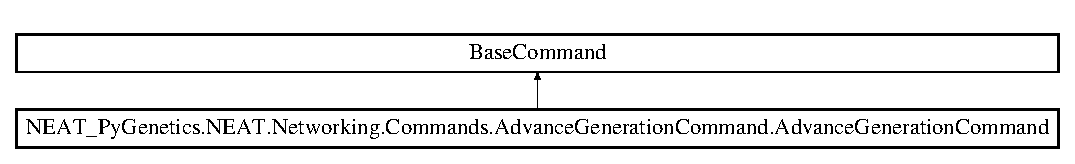
\includegraphics[height=1.758242cm]{classNEAT__PyGenetics_1_1NEAT_1_1Networking_1_1Commands_1_1AdvanceGenerationCommand_1_1AdvanceGenerationCommand}
\end{center}
\end{figure}
\subsection*{Public Member Functions}
\begin{DoxyCompactItemize}
\item 
def \hyperlink{classNEAT__PyGenetics_1_1NEAT_1_1Networking_1_1Commands_1_1AdvanceGenerationCommand_1_1AdvanceGenerationCommand_aa5c2d4cae5b431359a0563a53f2e8020}{\+\_\+\+\_\+init\+\_\+\+\_\+} (self)
\item 
def \hyperlink{classNEAT__PyGenetics_1_1NEAT_1_1Networking_1_1Commands_1_1AdvanceGenerationCommand_1_1AdvanceGenerationCommand_a2d1945cf45fc83a8fc73aa690829969d}{set\+\_\+advance\+\_\+generation}
\end{DoxyCompactItemize}


\subsection{Constructor \& Destructor Documentation}
\index{N\+E\+A\+T\+\_\+\+Py\+Genetics\+::\+N\+E\+A\+T\+::\+Networking\+::\+Commands\+::\+Advance\+Generation\+Command\+::\+Advance\+Generation\+Command@{N\+E\+A\+T\+\_\+\+Py\+Genetics\+::\+N\+E\+A\+T\+::\+Networking\+::\+Commands\+::\+Advance\+Generation\+Command\+::\+Advance\+Generation\+Command}!\+\_\+\+\_\+init\+\_\+\+\_\+@{\+\_\+\+\_\+init\+\_\+\+\_\+}}
\index{\+\_\+\+\_\+init\+\_\+\+\_\+@{\+\_\+\+\_\+init\+\_\+\+\_\+}!N\+E\+A\+T\+\_\+\+Py\+Genetics\+::\+N\+E\+A\+T\+::\+Networking\+::\+Commands\+::\+Advance\+Generation\+Command\+::\+Advance\+Generation\+Command@{N\+E\+A\+T\+\_\+\+Py\+Genetics\+::\+N\+E\+A\+T\+::\+Networking\+::\+Commands\+::\+Advance\+Generation\+Command\+::\+Advance\+Generation\+Command}}
\subsubsection[{\texorpdfstring{\+\_\+\+\_\+init\+\_\+\+\_\+(self)}{__init__(self)}}]{\setlength{\rightskip}{0pt plus 5cm}def N\+E\+A\+T\+\_\+\+Py\+Genetics.\+N\+E\+A\+T.\+Networking.\+Commands.\+Advance\+Generation\+Command.\+Advance\+Generation\+Command.\+\_\+\+\_\+init\+\_\+\+\_\+ (
\begin{DoxyParamCaption}
\item[{}]{self}
\end{DoxyParamCaption}
)}\hypertarget{classNEAT__PyGenetics_1_1NEAT_1_1Networking_1_1Commands_1_1AdvanceGenerationCommand_1_1AdvanceGenerationCommand_aa5c2d4cae5b431359a0563a53f2e8020}{}\label{classNEAT__PyGenetics_1_1NEAT_1_1Networking_1_1Commands_1_1AdvanceGenerationCommand_1_1AdvanceGenerationCommand_aa5c2d4cae5b431359a0563a53f2e8020}


\subsection{Member Function Documentation}
\index{N\+E\+A\+T\+\_\+\+Py\+Genetics\+::\+N\+E\+A\+T\+::\+Networking\+::\+Commands\+::\+Advance\+Generation\+Command\+::\+Advance\+Generation\+Command@{N\+E\+A\+T\+\_\+\+Py\+Genetics\+::\+N\+E\+A\+T\+::\+Networking\+::\+Commands\+::\+Advance\+Generation\+Command\+::\+Advance\+Generation\+Command}!set\+\_\+advance\+\_\+generation@{set\+\_\+advance\+\_\+generation}}
\index{set\+\_\+advance\+\_\+generation@{set\+\_\+advance\+\_\+generation}!N\+E\+A\+T\+\_\+\+Py\+Genetics\+::\+N\+E\+A\+T\+::\+Networking\+::\+Commands\+::\+Advance\+Generation\+Command\+::\+Advance\+Generation\+Command@{N\+E\+A\+T\+\_\+\+Py\+Genetics\+::\+N\+E\+A\+T\+::\+Networking\+::\+Commands\+::\+Advance\+Generation\+Command\+::\+Advance\+Generation\+Command}}
\subsubsection[{\texorpdfstring{set\+\_\+advance\+\_\+generation}{set_advance_generation}}]{\setlength{\rightskip}{0pt plus 5cm}def N\+E\+A\+T\+\_\+\+Py\+Genetics.\+N\+E\+A\+T.\+Networking.\+Commands.\+Advance\+Generation\+Command.\+Advance\+Generation\+Command.\+set\+\_\+advance\+\_\+generation (
\begin{DoxyParamCaption}
\item[{}]{self, }
\item[{}]{advance\+\_\+generation}
\end{DoxyParamCaption}
)}\hypertarget{classNEAT__PyGenetics_1_1NEAT_1_1Networking_1_1Commands_1_1AdvanceGenerationCommand_1_1AdvanceGenerationCommand_a2d1945cf45fc83a8fc73aa690829969d}{}\label{classNEAT__PyGenetics_1_1NEAT_1_1Networking_1_1Commands_1_1AdvanceGenerationCommand_1_1AdvanceGenerationCommand_a2d1945cf45fc83a8fc73aa690829969d}


The documentation for this class was generated from the following file\+:\begin{DoxyCompactItemize}
\item 
N\+E\+A\+T/\+Networking/\+Commands/\hyperlink{AdvanceGenerationCommand_8py}{Advance\+Generation\+Command.\+py}\end{DoxyCompactItemize}

\hypertarget{classNEAT__PyGenetics_1_1NEAT_1_1GenomeStructures_1_1AnalysisStructure_1_1AnalysisGenome_1_1AnalysisGenome}{}\section{N\+E\+A\+T\+\_\+\+Py\+Genetics.\+N\+E\+A\+T.\+Genome\+Structures.\+Analysis\+Structure.\+Analysis\+Genome.\+Analysis\+Genome Class Reference}
\label{classNEAT__PyGenetics_1_1NEAT_1_1GenomeStructures_1_1AnalysisStructure_1_1AnalysisGenome_1_1AnalysisGenome}\index{N\+E\+A\+T\+\_\+\+Py\+Genetics.\+N\+E\+A\+T.\+Genome\+Structures.\+Analysis\+Structure.\+Analysis\+Genome.\+Analysis\+Genome@{N\+E\+A\+T\+\_\+\+Py\+Genetics.\+N\+E\+A\+T.\+Genome\+Structures.\+Analysis\+Structure.\+Analysis\+Genome.\+Analysis\+Genome}}


Data structure used for analysing genome graphs.  


Inheritance diagram for N\+E\+A\+T\+\_\+\+Py\+Genetics.\+N\+E\+A\+T.\+Genome\+Structures.\+Analysis\+Structure.\+Analysis\+Genome.\+Analysis\+Genome\+:\begin{figure}[H]
\begin{center}
\leavevmode
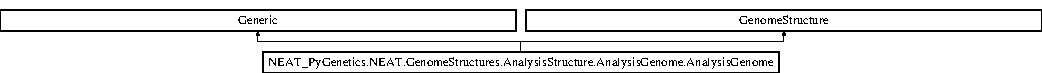
\includegraphics[height=0.984183cm]{classNEAT__PyGenetics_1_1NEAT_1_1GenomeStructures_1_1AnalysisStructure_1_1AnalysisGenome_1_1AnalysisGenome}
\end{center}
\end{figure}
\subsection*{Public Member Functions}
\begin{DoxyCompactItemize}
\item 
def \hyperlink{classNEAT__PyGenetics_1_1NEAT_1_1GenomeStructures_1_1AnalysisStructure_1_1AnalysisGenome_1_1AnalysisGenome_ade327b90f0ad5077a0864d5a7dfe705e}{\+\_\+\+\_\+init\+\_\+\+\_\+}
\begin{DoxyCompactList}\small\item\em Creates an \hyperlink{classNEAT__PyGenetics_1_1NEAT_1_1GenomeStructures_1_1AnalysisStructure_1_1AnalysisGenome_1_1AnalysisGenome}{Analysis\+Genome}. \end{DoxyCompactList}\item 
def \hyperlink{classNEAT__PyGenetics_1_1NEAT_1_1GenomeStructures_1_1AnalysisStructure_1_1AnalysisGenome_1_1AnalysisGenome_afde7a1abfb35596b72a79b5a1119acfd}{input\+\_\+nodes} (self)
\item 
def \hyperlink{classNEAT__PyGenetics_1_1NEAT_1_1GenomeStructures_1_1AnalysisStructure_1_1AnalysisGenome_1_1AnalysisGenome_afd38f7e3e579713434e6f7ad977ace57}{output\+\_\+nodes} (self)
\item 
def \hyperlink{classNEAT__PyGenetics_1_1NEAT_1_1GenomeStructures_1_1AnalysisStructure_1_1AnalysisGenome_1_1AnalysisGenome_a249bc4c5e9cbf9f5f4e9c7c4d6dcfc4b}{nodes} (self)
\item 
def \hyperlink{classNEAT__PyGenetics_1_1NEAT_1_1GenomeStructures_1_1AnalysisStructure_1_1AnalysisGenome_1_1AnalysisGenome_a4435fda98d49756abec987840f902abb}{edges} (self)
\item 
def \hyperlink{classNEAT__PyGenetics_1_1NEAT_1_1GenomeStructures_1_1AnalysisStructure_1_1AnalysisGenome_1_1AnalysisGenome_a0fead92350d58b2f5f078e7fa54e19e0}{initialised} (self)
\end{DoxyCompactItemize}
\subsection*{Static Public Attributes}
\begin{DoxyCompactItemize}
\item 
\hyperlink{classNEAT__PyGenetics_1_1NEAT_1_1GenomeStructures_1_1AnalysisStructure_1_1AnalysisGenome_1_1AnalysisGenome_a0738164ade43882c355f33037d133280}{head}
\item 
\hyperlink{classNEAT__PyGenetics_1_1NEAT_1_1GenomeStructures_1_1AnalysisStructure_1_1AnalysisGenome_1_1AnalysisGenome_a41704621b0d39e8476b95141dd1cf18d}{tail}
\end{DoxyCompactItemize}


\subsection{Detailed Description}
Data structure used for analysing genome graphs. 

It uses an adjacency list representation of the genome graph which is compatible with well known graph algorithms. 

\subsection{Constructor \& Destructor Documentation}
\index{N\+E\+A\+T\+\_\+\+Py\+Genetics\+::\+N\+E\+A\+T\+::\+Genome\+Structures\+::\+Analysis\+Structure\+::\+Analysis\+Genome\+::\+Analysis\+Genome@{N\+E\+A\+T\+\_\+\+Py\+Genetics\+::\+N\+E\+A\+T\+::\+Genome\+Structures\+::\+Analysis\+Structure\+::\+Analysis\+Genome\+::\+Analysis\+Genome}!\+\_\+\+\_\+init\+\_\+\+\_\+@{\+\_\+\+\_\+init\+\_\+\+\_\+}}
\index{\+\_\+\+\_\+init\+\_\+\+\_\+@{\+\_\+\+\_\+init\+\_\+\+\_\+}!N\+E\+A\+T\+\_\+\+Py\+Genetics\+::\+N\+E\+A\+T\+::\+Genome\+Structures\+::\+Analysis\+Structure\+::\+Analysis\+Genome\+::\+Analysis\+Genome@{N\+E\+A\+T\+\_\+\+Py\+Genetics\+::\+N\+E\+A\+T\+::\+Genome\+Structures\+::\+Analysis\+Structure\+::\+Analysis\+Genome\+::\+Analysis\+Genome}}
\subsubsection[{\texorpdfstring{\+\_\+\+\_\+init\+\_\+\+\_\+}{__init__}}]{\setlength{\rightskip}{0pt plus 5cm}def N\+E\+A\+T\+\_\+\+Py\+Genetics.\+N\+E\+A\+T.\+Genome\+Structures.\+Analysis\+Structure.\+Analysis\+Genome.\+Analysis\+Genome.\+\_\+\+\_\+init\+\_\+\+\_\+ (
\begin{DoxyParamCaption}
\item[{}]{self, }
\item[{}]{gene\+\_\+repository}
\end{DoxyParamCaption}
)}\hypertarget{classNEAT__PyGenetics_1_1NEAT_1_1GenomeStructures_1_1AnalysisStructure_1_1AnalysisGenome_1_1AnalysisGenome_ade327b90f0ad5077a0864d5a7dfe705e}{}\label{classNEAT__PyGenetics_1_1NEAT_1_1GenomeStructures_1_1AnalysisStructure_1_1AnalysisGenome_1_1AnalysisGenome_ade327b90f0ad5077a0864d5a7dfe705e}


Creates an \hyperlink{classNEAT__PyGenetics_1_1NEAT_1_1GenomeStructures_1_1AnalysisStructure_1_1AnalysisGenome_1_1AnalysisGenome}{Analysis\+Genome}. 

If a Storage\+Genome is given, it is used for construction. Otherwise the \hyperlink{classNEAT__PyGenetics_1_1NEAT_1_1GenomeStructures_1_1AnalysisStructure_1_1AnalysisGenome_1_1AnalysisGenome}{Analysis\+Genome} is constructed empty. \+:param gene\+\_\+repository\+: \+:param storage\+\_\+structure\+: \+:return\+: 

\subsection{Member Function Documentation}
\index{N\+E\+A\+T\+\_\+\+Py\+Genetics\+::\+N\+E\+A\+T\+::\+Genome\+Structures\+::\+Analysis\+Structure\+::\+Analysis\+Genome\+::\+Analysis\+Genome@{N\+E\+A\+T\+\_\+\+Py\+Genetics\+::\+N\+E\+A\+T\+::\+Genome\+Structures\+::\+Analysis\+Structure\+::\+Analysis\+Genome\+::\+Analysis\+Genome}!edges@{edges}}
\index{edges@{edges}!N\+E\+A\+T\+\_\+\+Py\+Genetics\+::\+N\+E\+A\+T\+::\+Genome\+Structures\+::\+Analysis\+Structure\+::\+Analysis\+Genome\+::\+Analysis\+Genome@{N\+E\+A\+T\+\_\+\+Py\+Genetics\+::\+N\+E\+A\+T\+::\+Genome\+Structures\+::\+Analysis\+Structure\+::\+Analysis\+Genome\+::\+Analysis\+Genome}}
\subsubsection[{\texorpdfstring{edges(self)}{edges(self)}}]{\setlength{\rightskip}{0pt plus 5cm}def N\+E\+A\+T\+\_\+\+Py\+Genetics.\+N\+E\+A\+T.\+Genome\+Structures.\+Analysis\+Structure.\+Analysis\+Genome.\+Analysis\+Genome.\+edges (
\begin{DoxyParamCaption}
\item[{}]{self, }
\item[{}]{Dict, }
\item[{}]{int, }
\item[{}]{List, }
\item[{}]{Tuple, }
\item[{}]{int, }
\item[{}]{int}
\end{DoxyParamCaption}
)}\hypertarget{classNEAT__PyGenetics_1_1NEAT_1_1GenomeStructures_1_1AnalysisStructure_1_1AnalysisGenome_1_1AnalysisGenome_a4435fda98d49756abec987840f902abb}{}\label{classNEAT__PyGenetics_1_1NEAT_1_1GenomeStructures_1_1AnalysisStructure_1_1AnalysisGenome_1_1AnalysisGenome_a4435fda98d49756abec987840f902abb}
\index{N\+E\+A\+T\+\_\+\+Py\+Genetics\+::\+N\+E\+A\+T\+::\+Genome\+Structures\+::\+Analysis\+Structure\+::\+Analysis\+Genome\+::\+Analysis\+Genome@{N\+E\+A\+T\+\_\+\+Py\+Genetics\+::\+N\+E\+A\+T\+::\+Genome\+Structures\+::\+Analysis\+Structure\+::\+Analysis\+Genome\+::\+Analysis\+Genome}!initialised@{initialised}}
\index{initialised@{initialised}!N\+E\+A\+T\+\_\+\+Py\+Genetics\+::\+N\+E\+A\+T\+::\+Genome\+Structures\+::\+Analysis\+Structure\+::\+Analysis\+Genome\+::\+Analysis\+Genome@{N\+E\+A\+T\+\_\+\+Py\+Genetics\+::\+N\+E\+A\+T\+::\+Genome\+Structures\+::\+Analysis\+Structure\+::\+Analysis\+Genome\+::\+Analysis\+Genome}}
\subsubsection[{\texorpdfstring{initialised(self)}{initialised(self)}}]{\setlength{\rightskip}{0pt plus 5cm}def N\+E\+A\+T\+\_\+\+Py\+Genetics.\+N\+E\+A\+T.\+Genome\+Structures.\+Analysis\+Structure.\+Analysis\+Genome.\+Analysis\+Genome.\+initialised (
\begin{DoxyParamCaption}
\item[{}]{self, }
\item[{}]{bool}
\end{DoxyParamCaption}
)}\hypertarget{classNEAT__PyGenetics_1_1NEAT_1_1GenomeStructures_1_1AnalysisStructure_1_1AnalysisGenome_1_1AnalysisGenome_a0fead92350d58b2f5f078e7fa54e19e0}{}\label{classNEAT__PyGenetics_1_1NEAT_1_1GenomeStructures_1_1AnalysisStructure_1_1AnalysisGenome_1_1AnalysisGenome_a0fead92350d58b2f5f078e7fa54e19e0}
\index{N\+E\+A\+T\+\_\+\+Py\+Genetics\+::\+N\+E\+A\+T\+::\+Genome\+Structures\+::\+Analysis\+Structure\+::\+Analysis\+Genome\+::\+Analysis\+Genome@{N\+E\+A\+T\+\_\+\+Py\+Genetics\+::\+N\+E\+A\+T\+::\+Genome\+Structures\+::\+Analysis\+Structure\+::\+Analysis\+Genome\+::\+Analysis\+Genome}!input\+\_\+nodes@{input\+\_\+nodes}}
\index{input\+\_\+nodes@{input\+\_\+nodes}!N\+E\+A\+T\+\_\+\+Py\+Genetics\+::\+N\+E\+A\+T\+::\+Genome\+Structures\+::\+Analysis\+Structure\+::\+Analysis\+Genome\+::\+Analysis\+Genome@{N\+E\+A\+T\+\_\+\+Py\+Genetics\+::\+N\+E\+A\+T\+::\+Genome\+Structures\+::\+Analysis\+Structure\+::\+Analysis\+Genome\+::\+Analysis\+Genome}}
\subsubsection[{\texorpdfstring{input\+\_\+nodes(self)}{input_nodes(self)}}]{\setlength{\rightskip}{0pt plus 5cm}def N\+E\+A\+T\+\_\+\+Py\+Genetics.\+N\+E\+A\+T.\+Genome\+Structures.\+Analysis\+Structure.\+Analysis\+Genome.\+Analysis\+Genome.\+input\+\_\+nodes (
\begin{DoxyParamCaption}
\item[{}]{self, }
\item[{}]{Dict, }
\item[{}]{str, }
\item[{}]{int}
\end{DoxyParamCaption}
)}\hypertarget{classNEAT__PyGenetics_1_1NEAT_1_1GenomeStructures_1_1AnalysisStructure_1_1AnalysisGenome_1_1AnalysisGenome_afde7a1abfb35596b72a79b5a1119acfd}{}\label{classNEAT__PyGenetics_1_1NEAT_1_1GenomeStructures_1_1AnalysisStructure_1_1AnalysisGenome_1_1AnalysisGenome_afde7a1abfb35596b72a79b5a1119acfd}
\index{N\+E\+A\+T\+\_\+\+Py\+Genetics\+::\+N\+E\+A\+T\+::\+Genome\+Structures\+::\+Analysis\+Structure\+::\+Analysis\+Genome\+::\+Analysis\+Genome@{N\+E\+A\+T\+\_\+\+Py\+Genetics\+::\+N\+E\+A\+T\+::\+Genome\+Structures\+::\+Analysis\+Structure\+::\+Analysis\+Genome\+::\+Analysis\+Genome}!nodes@{nodes}}
\index{nodes@{nodes}!N\+E\+A\+T\+\_\+\+Py\+Genetics\+::\+N\+E\+A\+T\+::\+Genome\+Structures\+::\+Analysis\+Structure\+::\+Analysis\+Genome\+::\+Analysis\+Genome@{N\+E\+A\+T\+\_\+\+Py\+Genetics\+::\+N\+E\+A\+T\+::\+Genome\+Structures\+::\+Analysis\+Structure\+::\+Analysis\+Genome\+::\+Analysis\+Genome}}
\subsubsection[{\texorpdfstring{nodes(self)}{nodes(self)}}]{\setlength{\rightskip}{0pt plus 5cm}def N\+E\+A\+T\+\_\+\+Py\+Genetics.\+N\+E\+A\+T.\+Genome\+Structures.\+Analysis\+Structure.\+Analysis\+Genome.\+Analysis\+Genome.\+nodes (
\begin{DoxyParamCaption}
\item[{}]{self, }
\item[{}]{Set, }
\item[{}]{int}
\end{DoxyParamCaption}
)}\hypertarget{classNEAT__PyGenetics_1_1NEAT_1_1GenomeStructures_1_1AnalysisStructure_1_1AnalysisGenome_1_1AnalysisGenome_a249bc4c5e9cbf9f5f4e9c7c4d6dcfc4b}{}\label{classNEAT__PyGenetics_1_1NEAT_1_1GenomeStructures_1_1AnalysisStructure_1_1AnalysisGenome_1_1AnalysisGenome_a249bc4c5e9cbf9f5f4e9c7c4d6dcfc4b}
\index{N\+E\+A\+T\+\_\+\+Py\+Genetics\+::\+N\+E\+A\+T\+::\+Genome\+Structures\+::\+Analysis\+Structure\+::\+Analysis\+Genome\+::\+Analysis\+Genome@{N\+E\+A\+T\+\_\+\+Py\+Genetics\+::\+N\+E\+A\+T\+::\+Genome\+Structures\+::\+Analysis\+Structure\+::\+Analysis\+Genome\+::\+Analysis\+Genome}!output\+\_\+nodes@{output\+\_\+nodes}}
\index{output\+\_\+nodes@{output\+\_\+nodes}!N\+E\+A\+T\+\_\+\+Py\+Genetics\+::\+N\+E\+A\+T\+::\+Genome\+Structures\+::\+Analysis\+Structure\+::\+Analysis\+Genome\+::\+Analysis\+Genome@{N\+E\+A\+T\+\_\+\+Py\+Genetics\+::\+N\+E\+A\+T\+::\+Genome\+Structures\+::\+Analysis\+Structure\+::\+Analysis\+Genome\+::\+Analysis\+Genome}}
\subsubsection[{\texorpdfstring{output\+\_\+nodes(self)}{output_nodes(self)}}]{\setlength{\rightskip}{0pt plus 5cm}def N\+E\+A\+T\+\_\+\+Py\+Genetics.\+N\+E\+A\+T.\+Genome\+Structures.\+Analysis\+Structure.\+Analysis\+Genome.\+Analysis\+Genome.\+output\+\_\+nodes (
\begin{DoxyParamCaption}
\item[{}]{self, }
\item[{}]{Dict, }
\item[{}]{str, }
\item[{}]{int}
\end{DoxyParamCaption}
)}\hypertarget{classNEAT__PyGenetics_1_1NEAT_1_1GenomeStructures_1_1AnalysisStructure_1_1AnalysisGenome_1_1AnalysisGenome_afd38f7e3e579713434e6f7ad977ace57}{}\label{classNEAT__PyGenetics_1_1NEAT_1_1GenomeStructures_1_1AnalysisStructure_1_1AnalysisGenome_1_1AnalysisGenome_afd38f7e3e579713434e6f7ad977ace57}


\subsection{Member Data Documentation}
\index{N\+E\+A\+T\+\_\+\+Py\+Genetics\+::\+N\+E\+A\+T\+::\+Genome\+Structures\+::\+Analysis\+Structure\+::\+Analysis\+Genome\+::\+Analysis\+Genome@{N\+E\+A\+T\+\_\+\+Py\+Genetics\+::\+N\+E\+A\+T\+::\+Genome\+Structures\+::\+Analysis\+Structure\+::\+Analysis\+Genome\+::\+Analysis\+Genome}!head@{head}}
\index{head@{head}!N\+E\+A\+T\+\_\+\+Py\+Genetics\+::\+N\+E\+A\+T\+::\+Genome\+Structures\+::\+Analysis\+Structure\+::\+Analysis\+Genome\+::\+Analysis\+Genome@{N\+E\+A\+T\+\_\+\+Py\+Genetics\+::\+N\+E\+A\+T\+::\+Genome\+Structures\+::\+Analysis\+Structure\+::\+Analysis\+Genome\+::\+Analysis\+Genome}}
\subsubsection[{\texorpdfstring{head}{head}}]{\setlength{\rightskip}{0pt plus 5cm}N\+E\+A\+T\+\_\+\+Py\+Genetics.\+N\+E\+A\+T.\+Genome\+Structures.\+Analysis\+Structure.\+Analysis\+Genome.\+Analysis\+Genome.\+head\hspace{0.3cm}{\ttfamily [static]}}\hypertarget{classNEAT__PyGenetics_1_1NEAT_1_1GenomeStructures_1_1AnalysisStructure_1_1AnalysisGenome_1_1AnalysisGenome_a0738164ade43882c355f33037d133280}{}\label{classNEAT__PyGenetics_1_1NEAT_1_1GenomeStructures_1_1AnalysisStructure_1_1AnalysisGenome_1_1AnalysisGenome_a0738164ade43882c355f33037d133280}
\index{N\+E\+A\+T\+\_\+\+Py\+Genetics\+::\+N\+E\+A\+T\+::\+Genome\+Structures\+::\+Analysis\+Structure\+::\+Analysis\+Genome\+::\+Analysis\+Genome@{N\+E\+A\+T\+\_\+\+Py\+Genetics\+::\+N\+E\+A\+T\+::\+Genome\+Structures\+::\+Analysis\+Structure\+::\+Analysis\+Genome\+::\+Analysis\+Genome}!tail@{tail}}
\index{tail@{tail}!N\+E\+A\+T\+\_\+\+Py\+Genetics\+::\+N\+E\+A\+T\+::\+Genome\+Structures\+::\+Analysis\+Structure\+::\+Analysis\+Genome\+::\+Analysis\+Genome@{N\+E\+A\+T\+\_\+\+Py\+Genetics\+::\+N\+E\+A\+T\+::\+Genome\+Structures\+::\+Analysis\+Structure\+::\+Analysis\+Genome\+::\+Analysis\+Genome}}
\subsubsection[{\texorpdfstring{tail}{tail}}]{\setlength{\rightskip}{0pt plus 5cm}N\+E\+A\+T\+\_\+\+Py\+Genetics.\+N\+E\+A\+T.\+Genome\+Structures.\+Analysis\+Structure.\+Analysis\+Genome.\+Analysis\+Genome.\+tail\hspace{0.3cm}{\ttfamily [static]}}\hypertarget{classNEAT__PyGenetics_1_1NEAT_1_1GenomeStructures_1_1AnalysisStructure_1_1AnalysisGenome_1_1AnalysisGenome_a41704621b0d39e8476b95141dd1cf18d}{}\label{classNEAT__PyGenetics_1_1NEAT_1_1GenomeStructures_1_1AnalysisStructure_1_1AnalysisGenome_1_1AnalysisGenome_a41704621b0d39e8476b95141dd1cf18d}


The documentation for this class was generated from the following file\+:\begin{DoxyCompactItemize}
\item 
N\+E\+A\+T/\+Genome\+Structures/\+Analysis\+Structure/\hyperlink{AnalysisGenome_8py}{Analysis\+Genome.\+py}\end{DoxyCompactItemize}

\hypertarget{classNEAT__PyGenetics_1_1NEAT_1_1Analyst_1_1AnalysisResult_1_1AnalysisResult}{}\section{N\+E\+A\+T\+\_\+\+Py\+Genetics.\+N\+E\+A\+T.\+Analyst.\+Analysis\+Result.\+Analysis\+Result Class Reference}
\label{classNEAT__PyGenetics_1_1NEAT_1_1Analyst_1_1AnalysisResult_1_1AnalysisResult}\index{N\+E\+A\+T\+\_\+\+Py\+Genetics.\+N\+E\+A\+T.\+Analyst.\+Analysis\+Result.\+Analysis\+Result@{N\+E\+A\+T\+\_\+\+Py\+Genetics.\+N\+E\+A\+T.\+Analyst.\+Analysis\+Result.\+Analysis\+Result}}


Object used to store results of graph analysis.  


Inheritance diagram for N\+E\+A\+T\+\_\+\+Py\+Genetics.\+N\+E\+A\+T.\+Analyst.\+Analysis\+Result.\+Analysis\+Result\+:\begin{figure}[H]
\begin{center}
\leavevmode
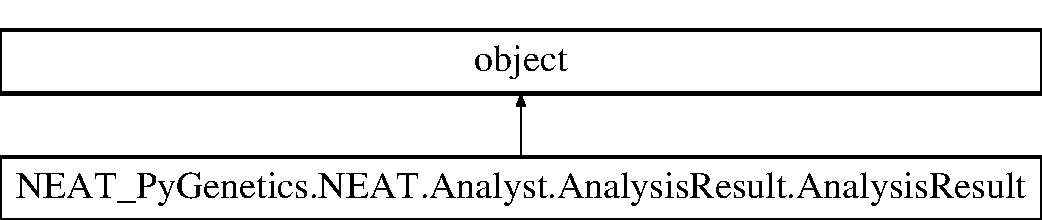
\includegraphics[height=2.000000cm]{classNEAT__PyGenetics_1_1NEAT_1_1Analyst_1_1AnalysisResult_1_1AnalysisResult}
\end{center}
\end{figure}
\subsection*{Public Member Functions}
\begin{DoxyCompactItemize}
\item 
def \hyperlink{classNEAT__PyGenetics_1_1NEAT_1_1Analyst_1_1AnalysisResult_1_1AnalysisResult_a76e2ba4c3bec7e93ab1c78e281a8504d}{\+\_\+\+\_\+init\+\_\+\+\_\+}
\begin{DoxyCompactList}\small\item\em \+:param analysis\+\_\+result\+: If analysis\+\_\+result is given, its contents are copied. \end{DoxyCompactList}\item 
def \hyperlink{classNEAT__PyGenetics_1_1NEAT_1_1Analyst_1_1AnalysisResult_1_1AnalysisResult_a6145154aa0f23413e57312a78cc12f91}{\+\_\+\+\_\+eq\+\_\+\+\_\+}
\item 
def \hyperlink{classNEAT__PyGenetics_1_1NEAT_1_1Analyst_1_1AnalysisResult_1_1AnalysisResult_abc4627be334a397f27b8173cb4a21796}{clear} (self)
\item 
def \hyperlink{classNEAT__PyGenetics_1_1NEAT_1_1Analyst_1_1AnalysisResult_1_1AnalysisResult_ad3a9bbe518536d18882346d8ee9dd28e}{cycle\+\_\+nodes} (self)
\end{DoxyCompactItemize}
\subsection*{Public Attributes}
\begin{DoxyCompactItemize}
\item 
\hyperlink{classNEAT__PyGenetics_1_1NEAT_1_1Analyst_1_1AnalysisResult_1_1AnalysisResult_a8ad8be788715b6298240055bbd835d5e}{gene\+\_\+closes\+\_\+cycle\+\_\+map}
\item 
\hyperlink{classNEAT__PyGenetics_1_1NEAT_1_1Analyst_1_1AnalysisResult_1_1AnalysisResult_a5dec17c624dfc418d21b543b366413e2}{topologically\+\_\+sorted\+\_\+nodes}
\item 
\hyperlink{classNEAT__PyGenetics_1_1NEAT_1_1Analyst_1_1AnalysisResult_1_1AnalysisResult_acca98f28e97dddad4c4ee0c86d499e58}{topologically\+\_\+sorted\+\_\+cycle\+\_\+nodes}
\end{DoxyCompactItemize}


\subsection{Detailed Description}
Object used to store results of graph analysis. 

Attributes\+: gene\+\_\+closes\+\_\+cycle\+\_\+map\+: a dict that consists of gene id\textquotesingle{}s (ints) as keys a boolean value that is true, if the gene closes a circle in the a-\/ nalyzed graph. topologically\+\_\+sorted\+\_\+nodes\+: a list of all nodes in the analyzed graph in topological order. topologically\+\_\+sorted\+\_\+cycle\+\_\+nodes\+: a list of all cycle closing nodes (at the source of the closing edge) in topological order. This is a sub-\/ set of topologically\+\_\+sorted\+\_\+nodes. 

\subsection{Constructor \& Destructor Documentation}
\index{N\+E\+A\+T\+\_\+\+Py\+Genetics\+::\+N\+E\+A\+T\+::\+Analyst\+::\+Analysis\+Result\+::\+Analysis\+Result@{N\+E\+A\+T\+\_\+\+Py\+Genetics\+::\+N\+E\+A\+T\+::\+Analyst\+::\+Analysis\+Result\+::\+Analysis\+Result}!\+\_\+\+\_\+init\+\_\+\+\_\+@{\+\_\+\+\_\+init\+\_\+\+\_\+}}
\index{\+\_\+\+\_\+init\+\_\+\+\_\+@{\+\_\+\+\_\+init\+\_\+\+\_\+}!N\+E\+A\+T\+\_\+\+Py\+Genetics\+::\+N\+E\+A\+T\+::\+Analyst\+::\+Analysis\+Result\+::\+Analysis\+Result@{N\+E\+A\+T\+\_\+\+Py\+Genetics\+::\+N\+E\+A\+T\+::\+Analyst\+::\+Analysis\+Result\+::\+Analysis\+Result}}
\subsubsection[{\texorpdfstring{\+\_\+\+\_\+init\+\_\+\+\_\+}{__init__}}]{\setlength{\rightskip}{0pt plus 5cm}def N\+E\+A\+T\+\_\+\+Py\+Genetics.\+N\+E\+A\+T.\+Analyst.\+Analysis\+Result.\+Analysis\+Result.\+\_\+\+\_\+init\+\_\+\+\_\+ (
\begin{DoxyParamCaption}
\item[{}]{self, }
\item[{}]{analysis\+\_\+result}
\end{DoxyParamCaption}
)}\hypertarget{classNEAT__PyGenetics_1_1NEAT_1_1Analyst_1_1AnalysisResult_1_1AnalysisResult_a76e2ba4c3bec7e93ab1c78e281a8504d}{}\label{classNEAT__PyGenetics_1_1NEAT_1_1Analyst_1_1AnalysisResult_1_1AnalysisResult_a76e2ba4c3bec7e93ab1c78e281a8504d}


\+:param analysis\+\_\+result\+: If analysis\+\_\+result is given, its contents are copied. 

\+:return\+: 

\subsection{Member Function Documentation}
\index{N\+E\+A\+T\+\_\+\+Py\+Genetics\+::\+N\+E\+A\+T\+::\+Analyst\+::\+Analysis\+Result\+::\+Analysis\+Result@{N\+E\+A\+T\+\_\+\+Py\+Genetics\+::\+N\+E\+A\+T\+::\+Analyst\+::\+Analysis\+Result\+::\+Analysis\+Result}!\+\_\+\+\_\+eq\+\_\+\+\_\+@{\+\_\+\+\_\+eq\+\_\+\+\_\+}}
\index{\+\_\+\+\_\+eq\+\_\+\+\_\+@{\+\_\+\+\_\+eq\+\_\+\+\_\+}!N\+E\+A\+T\+\_\+\+Py\+Genetics\+::\+N\+E\+A\+T\+::\+Analyst\+::\+Analysis\+Result\+::\+Analysis\+Result@{N\+E\+A\+T\+\_\+\+Py\+Genetics\+::\+N\+E\+A\+T\+::\+Analyst\+::\+Analysis\+Result\+::\+Analysis\+Result}}
\subsubsection[{\texorpdfstring{\+\_\+\+\_\+eq\+\_\+\+\_\+}{__eq__}}]{\setlength{\rightskip}{0pt plus 5cm}def N\+E\+A\+T\+\_\+\+Py\+Genetics.\+N\+E\+A\+T.\+Analyst.\+Analysis\+Result.\+Analysis\+Result.\+\_\+\+\_\+eq\+\_\+\+\_\+ (
\begin{DoxyParamCaption}
\item[{}]{self, }
\item[{}]{obj}
\end{DoxyParamCaption}
)}\hypertarget{classNEAT__PyGenetics_1_1NEAT_1_1Analyst_1_1AnalysisResult_1_1AnalysisResult_a6145154aa0f23413e57312a78cc12f91}{}\label{classNEAT__PyGenetics_1_1NEAT_1_1Analyst_1_1AnalysisResult_1_1AnalysisResult_a6145154aa0f23413e57312a78cc12f91}
\index{N\+E\+A\+T\+\_\+\+Py\+Genetics\+::\+N\+E\+A\+T\+::\+Analyst\+::\+Analysis\+Result\+::\+Analysis\+Result@{N\+E\+A\+T\+\_\+\+Py\+Genetics\+::\+N\+E\+A\+T\+::\+Analyst\+::\+Analysis\+Result\+::\+Analysis\+Result}!clear@{clear}}
\index{clear@{clear}!N\+E\+A\+T\+\_\+\+Py\+Genetics\+::\+N\+E\+A\+T\+::\+Analyst\+::\+Analysis\+Result\+::\+Analysis\+Result@{N\+E\+A\+T\+\_\+\+Py\+Genetics\+::\+N\+E\+A\+T\+::\+Analyst\+::\+Analysis\+Result\+::\+Analysis\+Result}}
\subsubsection[{\texorpdfstring{clear(self)}{clear(self)}}]{\setlength{\rightskip}{0pt plus 5cm}def N\+E\+A\+T\+\_\+\+Py\+Genetics.\+N\+E\+A\+T.\+Analyst.\+Analysis\+Result.\+Analysis\+Result.\+clear (
\begin{DoxyParamCaption}
\item[{}]{self, }
\item[{}]{None}
\end{DoxyParamCaption}
)}\hypertarget{classNEAT__PyGenetics_1_1NEAT_1_1Analyst_1_1AnalysisResult_1_1AnalysisResult_abc4627be334a397f27b8173cb4a21796}{}\label{classNEAT__PyGenetics_1_1NEAT_1_1Analyst_1_1AnalysisResult_1_1AnalysisResult_abc4627be334a397f27b8173cb4a21796}
\index{N\+E\+A\+T\+\_\+\+Py\+Genetics\+::\+N\+E\+A\+T\+::\+Analyst\+::\+Analysis\+Result\+::\+Analysis\+Result@{N\+E\+A\+T\+\_\+\+Py\+Genetics\+::\+N\+E\+A\+T\+::\+Analyst\+::\+Analysis\+Result\+::\+Analysis\+Result}!cycle\+\_\+nodes@{cycle\+\_\+nodes}}
\index{cycle\+\_\+nodes@{cycle\+\_\+nodes}!N\+E\+A\+T\+\_\+\+Py\+Genetics\+::\+N\+E\+A\+T\+::\+Analyst\+::\+Analysis\+Result\+::\+Analysis\+Result@{N\+E\+A\+T\+\_\+\+Py\+Genetics\+::\+N\+E\+A\+T\+::\+Analyst\+::\+Analysis\+Result\+::\+Analysis\+Result}}
\subsubsection[{\texorpdfstring{cycle\+\_\+nodes(self)}{cycle_nodes(self)}}]{\setlength{\rightskip}{0pt plus 5cm}def N\+E\+A\+T\+\_\+\+Py\+Genetics.\+N\+E\+A\+T.\+Analyst.\+Analysis\+Result.\+Analysis\+Result.\+cycle\+\_\+nodes (
\begin{DoxyParamCaption}
\item[{}]{self, }
\item[{}]{Set, }
\item[{}]{int}
\end{DoxyParamCaption}
)}\hypertarget{classNEAT__PyGenetics_1_1NEAT_1_1Analyst_1_1AnalysisResult_1_1AnalysisResult_ad3a9bbe518536d18882346d8ee9dd28e}{}\label{classNEAT__PyGenetics_1_1NEAT_1_1Analyst_1_1AnalysisResult_1_1AnalysisResult_ad3a9bbe518536d18882346d8ee9dd28e}


\subsection{Member Data Documentation}
\index{N\+E\+A\+T\+\_\+\+Py\+Genetics\+::\+N\+E\+A\+T\+::\+Analyst\+::\+Analysis\+Result\+::\+Analysis\+Result@{N\+E\+A\+T\+\_\+\+Py\+Genetics\+::\+N\+E\+A\+T\+::\+Analyst\+::\+Analysis\+Result\+::\+Analysis\+Result}!gene\+\_\+closes\+\_\+cycle\+\_\+map@{gene\+\_\+closes\+\_\+cycle\+\_\+map}}
\index{gene\+\_\+closes\+\_\+cycle\+\_\+map@{gene\+\_\+closes\+\_\+cycle\+\_\+map}!N\+E\+A\+T\+\_\+\+Py\+Genetics\+::\+N\+E\+A\+T\+::\+Analyst\+::\+Analysis\+Result\+::\+Analysis\+Result@{N\+E\+A\+T\+\_\+\+Py\+Genetics\+::\+N\+E\+A\+T\+::\+Analyst\+::\+Analysis\+Result\+::\+Analysis\+Result}}
\subsubsection[{\texorpdfstring{gene\+\_\+closes\+\_\+cycle\+\_\+map}{gene_closes_cycle_map}}]{\setlength{\rightskip}{0pt plus 5cm}N\+E\+A\+T\+\_\+\+Py\+Genetics.\+N\+E\+A\+T.\+Analyst.\+Analysis\+Result.\+Analysis\+Result.\+gene\+\_\+closes\+\_\+cycle\+\_\+map}\hypertarget{classNEAT__PyGenetics_1_1NEAT_1_1Analyst_1_1AnalysisResult_1_1AnalysisResult_a8ad8be788715b6298240055bbd835d5e}{}\label{classNEAT__PyGenetics_1_1NEAT_1_1Analyst_1_1AnalysisResult_1_1AnalysisResult_a8ad8be788715b6298240055bbd835d5e}
\index{N\+E\+A\+T\+\_\+\+Py\+Genetics\+::\+N\+E\+A\+T\+::\+Analyst\+::\+Analysis\+Result\+::\+Analysis\+Result@{N\+E\+A\+T\+\_\+\+Py\+Genetics\+::\+N\+E\+A\+T\+::\+Analyst\+::\+Analysis\+Result\+::\+Analysis\+Result}!topologically\+\_\+sorted\+\_\+cycle\+\_\+nodes@{topologically\+\_\+sorted\+\_\+cycle\+\_\+nodes}}
\index{topologically\+\_\+sorted\+\_\+cycle\+\_\+nodes@{topologically\+\_\+sorted\+\_\+cycle\+\_\+nodes}!N\+E\+A\+T\+\_\+\+Py\+Genetics\+::\+N\+E\+A\+T\+::\+Analyst\+::\+Analysis\+Result\+::\+Analysis\+Result@{N\+E\+A\+T\+\_\+\+Py\+Genetics\+::\+N\+E\+A\+T\+::\+Analyst\+::\+Analysis\+Result\+::\+Analysis\+Result}}
\subsubsection[{\texorpdfstring{topologically\+\_\+sorted\+\_\+cycle\+\_\+nodes}{topologically_sorted_cycle_nodes}}]{\setlength{\rightskip}{0pt plus 5cm}N\+E\+A\+T\+\_\+\+Py\+Genetics.\+N\+E\+A\+T.\+Analyst.\+Analysis\+Result.\+Analysis\+Result.\+topologically\+\_\+sorted\+\_\+cycle\+\_\+nodes}\hypertarget{classNEAT__PyGenetics_1_1NEAT_1_1Analyst_1_1AnalysisResult_1_1AnalysisResult_acca98f28e97dddad4c4ee0c86d499e58}{}\label{classNEAT__PyGenetics_1_1NEAT_1_1Analyst_1_1AnalysisResult_1_1AnalysisResult_acca98f28e97dddad4c4ee0c86d499e58}
\index{N\+E\+A\+T\+\_\+\+Py\+Genetics\+::\+N\+E\+A\+T\+::\+Analyst\+::\+Analysis\+Result\+::\+Analysis\+Result@{N\+E\+A\+T\+\_\+\+Py\+Genetics\+::\+N\+E\+A\+T\+::\+Analyst\+::\+Analysis\+Result\+::\+Analysis\+Result}!topologically\+\_\+sorted\+\_\+nodes@{topologically\+\_\+sorted\+\_\+nodes}}
\index{topologically\+\_\+sorted\+\_\+nodes@{topologically\+\_\+sorted\+\_\+nodes}!N\+E\+A\+T\+\_\+\+Py\+Genetics\+::\+N\+E\+A\+T\+::\+Analyst\+::\+Analysis\+Result\+::\+Analysis\+Result@{N\+E\+A\+T\+\_\+\+Py\+Genetics\+::\+N\+E\+A\+T\+::\+Analyst\+::\+Analysis\+Result\+::\+Analysis\+Result}}
\subsubsection[{\texorpdfstring{topologically\+\_\+sorted\+\_\+nodes}{topologically_sorted_nodes}}]{\setlength{\rightskip}{0pt plus 5cm}N\+E\+A\+T\+\_\+\+Py\+Genetics.\+N\+E\+A\+T.\+Analyst.\+Analysis\+Result.\+Analysis\+Result.\+topologically\+\_\+sorted\+\_\+nodes}\hypertarget{classNEAT__PyGenetics_1_1NEAT_1_1Analyst_1_1AnalysisResult_1_1AnalysisResult_a5dec17c624dfc418d21b543b366413e2}{}\label{classNEAT__PyGenetics_1_1NEAT_1_1Analyst_1_1AnalysisResult_1_1AnalysisResult_a5dec17c624dfc418d21b543b366413e2}


The documentation for this class was generated from the following file\+:\begin{DoxyCompactItemize}
\item 
N\+E\+A\+T/\+Analyst/\hyperlink{AnalysisResult_8py}{Analysis\+Result.\+py}\end{DoxyCompactItemize}

\hypertarget{classNEAT__PyGenetics_1_1NEAT_1_1Networking_1_1Commands_1_1AnnounceSessionCommand_1_1AnnounceSessionCommand}{}\section{N\+E\+A\+T\+\_\+\+Py\+Genetics.\+N\+E\+A\+T.\+Networking.\+Commands.\+Announce\+Session\+Command.\+Announce\+Session\+Command Class Reference}
\label{classNEAT__PyGenetics_1_1NEAT_1_1Networking_1_1Commands_1_1AnnounceSessionCommand_1_1AnnounceSessionCommand}\index{N\+E\+A\+T\+\_\+\+Py\+Genetics.\+N\+E\+A\+T.\+Networking.\+Commands.\+Announce\+Session\+Command.\+Announce\+Session\+Command@{N\+E\+A\+T\+\_\+\+Py\+Genetics.\+N\+E\+A\+T.\+Networking.\+Commands.\+Announce\+Session\+Command.\+Announce\+Session\+Command}}
Inheritance diagram for N\+E\+A\+T\+\_\+\+Py\+Genetics.\+N\+E\+A\+T.\+Networking.\+Commands.\+Announce\+Session\+Command.\+Announce\+Session\+Command\+:\begin{figure}[H]
\begin{center}
\leavevmode
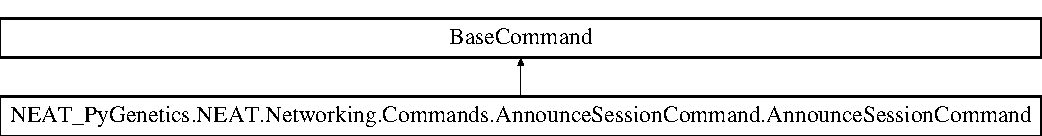
\includegraphics[height=1.821138cm]{classNEAT__PyGenetics_1_1NEAT_1_1Networking_1_1Commands_1_1AnnounceSessionCommand_1_1AnnounceSessionCommand}
\end{center}
\end{figure}
\subsection*{Public Member Functions}
\begin{DoxyCompactItemize}
\item 
def \hyperlink{classNEAT__PyGenetics_1_1NEAT_1_1Networking_1_1Commands_1_1AnnounceSessionCommand_1_1AnnounceSessionCommand_a9ac1c2d236b717bc4b7ec521a7f3daa5}{\+\_\+\+\_\+init\+\_\+\+\_\+} (self)
\item 
def \hyperlink{classNEAT__PyGenetics_1_1NEAT_1_1Networking_1_1Commands_1_1AnnounceSessionCommand_1_1AnnounceSessionCommand_ace39d5d011d61bb501f16f78ae1b4997}{set\+\_\+config\+\_\+path} (self, config\+\_\+path)
\item 
def \hyperlink{classNEAT__PyGenetics_1_1NEAT_1_1Networking_1_1Commands_1_1AnnounceSessionCommand_1_1AnnounceSessionCommand_ade8f205209da28a137c8d361a4830c0b}{get\+\_\+config\+\_\+path} (self)
\item 
def \hyperlink{classNEAT__PyGenetics_1_1NEAT_1_1Networking_1_1Commands_1_1AnnounceSessionCommand_1_1AnnounceSessionCommand_a7c9eae1dc5ba08c0b44182a6db99fd27}{set\+\_\+session\+\_\+id} (self, session\+\_\+id)
\item 
def \hyperlink{classNEAT__PyGenetics_1_1NEAT_1_1Networking_1_1Commands_1_1AnnounceSessionCommand_1_1AnnounceSessionCommand_a3e3a2c23ea1b303a4892f77895dd9350}{get\+\_\+session\+\_\+id} (self)
\item 
def \hyperlink{classNEAT__PyGenetics_1_1NEAT_1_1Networking_1_1Commands_1_1AnnounceSessionCommand_1_1AnnounceSessionCommand_a4b4d1a2f45cbe7e4be0658a3751e9dc3}{set\+\_\+block\+\_\+size}
\item 
def \hyperlink{classNEAT__PyGenetics_1_1NEAT_1_1Networking_1_1Commands_1_1AnnounceSessionCommand_1_1AnnounceSessionCommand_af6a3e5c83d5d990c909ef038272d797e}{get\+\_\+block\+\_\+size} (self)
\end{DoxyCompactItemize}


\subsection{Constructor \& Destructor Documentation}
\index{N\+E\+A\+T\+\_\+\+Py\+Genetics\+::\+N\+E\+A\+T\+::\+Networking\+::\+Commands\+::\+Announce\+Session\+Command\+::\+Announce\+Session\+Command@{N\+E\+A\+T\+\_\+\+Py\+Genetics\+::\+N\+E\+A\+T\+::\+Networking\+::\+Commands\+::\+Announce\+Session\+Command\+::\+Announce\+Session\+Command}!\+\_\+\+\_\+init\+\_\+\+\_\+@{\+\_\+\+\_\+init\+\_\+\+\_\+}}
\index{\+\_\+\+\_\+init\+\_\+\+\_\+@{\+\_\+\+\_\+init\+\_\+\+\_\+}!N\+E\+A\+T\+\_\+\+Py\+Genetics\+::\+N\+E\+A\+T\+::\+Networking\+::\+Commands\+::\+Announce\+Session\+Command\+::\+Announce\+Session\+Command@{N\+E\+A\+T\+\_\+\+Py\+Genetics\+::\+N\+E\+A\+T\+::\+Networking\+::\+Commands\+::\+Announce\+Session\+Command\+::\+Announce\+Session\+Command}}
\subsubsection[{\texorpdfstring{\+\_\+\+\_\+init\+\_\+\+\_\+(self)}{__init__(self)}}]{\setlength{\rightskip}{0pt plus 5cm}def N\+E\+A\+T\+\_\+\+Py\+Genetics.\+N\+E\+A\+T.\+Networking.\+Commands.\+Announce\+Session\+Command.\+Announce\+Session\+Command.\+\_\+\+\_\+init\+\_\+\+\_\+ (
\begin{DoxyParamCaption}
\item[{}]{self}
\end{DoxyParamCaption}
)}\hypertarget{classNEAT__PyGenetics_1_1NEAT_1_1Networking_1_1Commands_1_1AnnounceSessionCommand_1_1AnnounceSessionCommand_a9ac1c2d236b717bc4b7ec521a7f3daa5}{}\label{classNEAT__PyGenetics_1_1NEAT_1_1Networking_1_1Commands_1_1AnnounceSessionCommand_1_1AnnounceSessionCommand_a9ac1c2d236b717bc4b7ec521a7f3daa5}


\subsection{Member Function Documentation}
\index{N\+E\+A\+T\+\_\+\+Py\+Genetics\+::\+N\+E\+A\+T\+::\+Networking\+::\+Commands\+::\+Announce\+Session\+Command\+::\+Announce\+Session\+Command@{N\+E\+A\+T\+\_\+\+Py\+Genetics\+::\+N\+E\+A\+T\+::\+Networking\+::\+Commands\+::\+Announce\+Session\+Command\+::\+Announce\+Session\+Command}!get\+\_\+block\+\_\+size@{get\+\_\+block\+\_\+size}}
\index{get\+\_\+block\+\_\+size@{get\+\_\+block\+\_\+size}!N\+E\+A\+T\+\_\+\+Py\+Genetics\+::\+N\+E\+A\+T\+::\+Networking\+::\+Commands\+::\+Announce\+Session\+Command\+::\+Announce\+Session\+Command@{N\+E\+A\+T\+\_\+\+Py\+Genetics\+::\+N\+E\+A\+T\+::\+Networking\+::\+Commands\+::\+Announce\+Session\+Command\+::\+Announce\+Session\+Command}}
\subsubsection[{\texorpdfstring{get\+\_\+block\+\_\+size(self)}{get_block_size(self)}}]{\setlength{\rightskip}{0pt plus 5cm}def N\+E\+A\+T\+\_\+\+Py\+Genetics.\+N\+E\+A\+T.\+Networking.\+Commands.\+Announce\+Session\+Command.\+Announce\+Session\+Command.\+get\+\_\+block\+\_\+size (
\begin{DoxyParamCaption}
\item[{}]{self}
\end{DoxyParamCaption}
)}\hypertarget{classNEAT__PyGenetics_1_1NEAT_1_1Networking_1_1Commands_1_1AnnounceSessionCommand_1_1AnnounceSessionCommand_af6a3e5c83d5d990c909ef038272d797e}{}\label{classNEAT__PyGenetics_1_1NEAT_1_1Networking_1_1Commands_1_1AnnounceSessionCommand_1_1AnnounceSessionCommand_af6a3e5c83d5d990c909ef038272d797e}
\index{N\+E\+A\+T\+\_\+\+Py\+Genetics\+::\+N\+E\+A\+T\+::\+Networking\+::\+Commands\+::\+Announce\+Session\+Command\+::\+Announce\+Session\+Command@{N\+E\+A\+T\+\_\+\+Py\+Genetics\+::\+N\+E\+A\+T\+::\+Networking\+::\+Commands\+::\+Announce\+Session\+Command\+::\+Announce\+Session\+Command}!get\+\_\+config\+\_\+path@{get\+\_\+config\+\_\+path}}
\index{get\+\_\+config\+\_\+path@{get\+\_\+config\+\_\+path}!N\+E\+A\+T\+\_\+\+Py\+Genetics\+::\+N\+E\+A\+T\+::\+Networking\+::\+Commands\+::\+Announce\+Session\+Command\+::\+Announce\+Session\+Command@{N\+E\+A\+T\+\_\+\+Py\+Genetics\+::\+N\+E\+A\+T\+::\+Networking\+::\+Commands\+::\+Announce\+Session\+Command\+::\+Announce\+Session\+Command}}
\subsubsection[{\texorpdfstring{get\+\_\+config\+\_\+path(self)}{get_config_path(self)}}]{\setlength{\rightskip}{0pt plus 5cm}def N\+E\+A\+T\+\_\+\+Py\+Genetics.\+N\+E\+A\+T.\+Networking.\+Commands.\+Announce\+Session\+Command.\+Announce\+Session\+Command.\+get\+\_\+config\+\_\+path (
\begin{DoxyParamCaption}
\item[{}]{self}
\end{DoxyParamCaption}
)}\hypertarget{classNEAT__PyGenetics_1_1NEAT_1_1Networking_1_1Commands_1_1AnnounceSessionCommand_1_1AnnounceSessionCommand_ade8f205209da28a137c8d361a4830c0b}{}\label{classNEAT__PyGenetics_1_1NEAT_1_1Networking_1_1Commands_1_1AnnounceSessionCommand_1_1AnnounceSessionCommand_ade8f205209da28a137c8d361a4830c0b}
\index{N\+E\+A\+T\+\_\+\+Py\+Genetics\+::\+N\+E\+A\+T\+::\+Networking\+::\+Commands\+::\+Announce\+Session\+Command\+::\+Announce\+Session\+Command@{N\+E\+A\+T\+\_\+\+Py\+Genetics\+::\+N\+E\+A\+T\+::\+Networking\+::\+Commands\+::\+Announce\+Session\+Command\+::\+Announce\+Session\+Command}!get\+\_\+session\+\_\+id@{get\+\_\+session\+\_\+id}}
\index{get\+\_\+session\+\_\+id@{get\+\_\+session\+\_\+id}!N\+E\+A\+T\+\_\+\+Py\+Genetics\+::\+N\+E\+A\+T\+::\+Networking\+::\+Commands\+::\+Announce\+Session\+Command\+::\+Announce\+Session\+Command@{N\+E\+A\+T\+\_\+\+Py\+Genetics\+::\+N\+E\+A\+T\+::\+Networking\+::\+Commands\+::\+Announce\+Session\+Command\+::\+Announce\+Session\+Command}}
\subsubsection[{\texorpdfstring{get\+\_\+session\+\_\+id(self)}{get_session_id(self)}}]{\setlength{\rightskip}{0pt plus 5cm}def N\+E\+A\+T\+\_\+\+Py\+Genetics.\+N\+E\+A\+T.\+Networking.\+Commands.\+Announce\+Session\+Command.\+Announce\+Session\+Command.\+get\+\_\+session\+\_\+id (
\begin{DoxyParamCaption}
\item[{}]{self}
\end{DoxyParamCaption}
)}\hypertarget{classNEAT__PyGenetics_1_1NEAT_1_1Networking_1_1Commands_1_1AnnounceSessionCommand_1_1AnnounceSessionCommand_a3e3a2c23ea1b303a4892f77895dd9350}{}\label{classNEAT__PyGenetics_1_1NEAT_1_1Networking_1_1Commands_1_1AnnounceSessionCommand_1_1AnnounceSessionCommand_a3e3a2c23ea1b303a4892f77895dd9350}
\index{N\+E\+A\+T\+\_\+\+Py\+Genetics\+::\+N\+E\+A\+T\+::\+Networking\+::\+Commands\+::\+Announce\+Session\+Command\+::\+Announce\+Session\+Command@{N\+E\+A\+T\+\_\+\+Py\+Genetics\+::\+N\+E\+A\+T\+::\+Networking\+::\+Commands\+::\+Announce\+Session\+Command\+::\+Announce\+Session\+Command}!set\+\_\+block\+\_\+size@{set\+\_\+block\+\_\+size}}
\index{set\+\_\+block\+\_\+size@{set\+\_\+block\+\_\+size}!N\+E\+A\+T\+\_\+\+Py\+Genetics\+::\+N\+E\+A\+T\+::\+Networking\+::\+Commands\+::\+Announce\+Session\+Command\+::\+Announce\+Session\+Command@{N\+E\+A\+T\+\_\+\+Py\+Genetics\+::\+N\+E\+A\+T\+::\+Networking\+::\+Commands\+::\+Announce\+Session\+Command\+::\+Announce\+Session\+Command}}
\subsubsection[{\texorpdfstring{set\+\_\+block\+\_\+size}{set_block_size}}]{\setlength{\rightskip}{0pt plus 5cm}def N\+E\+A\+T\+\_\+\+Py\+Genetics.\+N\+E\+A\+T.\+Networking.\+Commands.\+Announce\+Session\+Command.\+Announce\+Session\+Command.\+set\+\_\+block\+\_\+size (
\begin{DoxyParamCaption}
\item[{}]{self, }
\item[{}]{block\+\_\+size}
\end{DoxyParamCaption}
)}\hypertarget{classNEAT__PyGenetics_1_1NEAT_1_1Networking_1_1Commands_1_1AnnounceSessionCommand_1_1AnnounceSessionCommand_a4b4d1a2f45cbe7e4be0658a3751e9dc3}{}\label{classNEAT__PyGenetics_1_1NEAT_1_1Networking_1_1Commands_1_1AnnounceSessionCommand_1_1AnnounceSessionCommand_a4b4d1a2f45cbe7e4be0658a3751e9dc3}
\index{N\+E\+A\+T\+\_\+\+Py\+Genetics\+::\+N\+E\+A\+T\+::\+Networking\+::\+Commands\+::\+Announce\+Session\+Command\+::\+Announce\+Session\+Command@{N\+E\+A\+T\+\_\+\+Py\+Genetics\+::\+N\+E\+A\+T\+::\+Networking\+::\+Commands\+::\+Announce\+Session\+Command\+::\+Announce\+Session\+Command}!set\+\_\+config\+\_\+path@{set\+\_\+config\+\_\+path}}
\index{set\+\_\+config\+\_\+path@{set\+\_\+config\+\_\+path}!N\+E\+A\+T\+\_\+\+Py\+Genetics\+::\+N\+E\+A\+T\+::\+Networking\+::\+Commands\+::\+Announce\+Session\+Command\+::\+Announce\+Session\+Command@{N\+E\+A\+T\+\_\+\+Py\+Genetics\+::\+N\+E\+A\+T\+::\+Networking\+::\+Commands\+::\+Announce\+Session\+Command\+::\+Announce\+Session\+Command}}
\subsubsection[{\texorpdfstring{set\+\_\+config\+\_\+path(self, config\+\_\+path)}{set_config_path(self, config_path)}}]{\setlength{\rightskip}{0pt plus 5cm}def N\+E\+A\+T\+\_\+\+Py\+Genetics.\+N\+E\+A\+T.\+Networking.\+Commands.\+Announce\+Session\+Command.\+Announce\+Session\+Command.\+set\+\_\+config\+\_\+path (
\begin{DoxyParamCaption}
\item[{}]{self, }
\item[{}]{config\+\_\+path}
\end{DoxyParamCaption}
)}\hypertarget{classNEAT__PyGenetics_1_1NEAT_1_1Networking_1_1Commands_1_1AnnounceSessionCommand_1_1AnnounceSessionCommand_ace39d5d011d61bb501f16f78ae1b4997}{}\label{classNEAT__PyGenetics_1_1NEAT_1_1Networking_1_1Commands_1_1AnnounceSessionCommand_1_1AnnounceSessionCommand_ace39d5d011d61bb501f16f78ae1b4997}
\index{N\+E\+A\+T\+\_\+\+Py\+Genetics\+::\+N\+E\+A\+T\+::\+Networking\+::\+Commands\+::\+Announce\+Session\+Command\+::\+Announce\+Session\+Command@{N\+E\+A\+T\+\_\+\+Py\+Genetics\+::\+N\+E\+A\+T\+::\+Networking\+::\+Commands\+::\+Announce\+Session\+Command\+::\+Announce\+Session\+Command}!set\+\_\+session\+\_\+id@{set\+\_\+session\+\_\+id}}
\index{set\+\_\+session\+\_\+id@{set\+\_\+session\+\_\+id}!N\+E\+A\+T\+\_\+\+Py\+Genetics\+::\+N\+E\+A\+T\+::\+Networking\+::\+Commands\+::\+Announce\+Session\+Command\+::\+Announce\+Session\+Command@{N\+E\+A\+T\+\_\+\+Py\+Genetics\+::\+N\+E\+A\+T\+::\+Networking\+::\+Commands\+::\+Announce\+Session\+Command\+::\+Announce\+Session\+Command}}
\subsubsection[{\texorpdfstring{set\+\_\+session\+\_\+id(self, session\+\_\+id)}{set_session_id(self, session_id)}}]{\setlength{\rightskip}{0pt plus 5cm}def N\+E\+A\+T\+\_\+\+Py\+Genetics.\+N\+E\+A\+T.\+Networking.\+Commands.\+Announce\+Session\+Command.\+Announce\+Session\+Command.\+set\+\_\+session\+\_\+id (
\begin{DoxyParamCaption}
\item[{}]{self, }
\item[{}]{session\+\_\+id}
\end{DoxyParamCaption}
)}\hypertarget{classNEAT__PyGenetics_1_1NEAT_1_1Networking_1_1Commands_1_1AnnounceSessionCommand_1_1AnnounceSessionCommand_a7c9eae1dc5ba08c0b44182a6db99fd27}{}\label{classNEAT__PyGenetics_1_1NEAT_1_1Networking_1_1Commands_1_1AnnounceSessionCommand_1_1AnnounceSessionCommand_a7c9eae1dc5ba08c0b44182a6db99fd27}


The documentation for this class was generated from the following file\+:\begin{DoxyCompactItemize}
\item 
N\+E\+A\+T/\+Networking/\+Commands/\hyperlink{AnnounceSessionCommand_8py}{Announce\+Session\+Command.\+py}\end{DoxyCompactItemize}

\hypertarget{classNEAT__PyGenetics_1_1NEAT_1_1Networking_1_1Commands_1_1BaseCommand_1_1BaseCommand}{}\section{N\+E\+A\+T\+\_\+\+Py\+Genetics.\+N\+E\+A\+T.\+Networking.\+Commands.\+Base\+Command.\+Base\+Command Class Reference}
\label{classNEAT__PyGenetics_1_1NEAT_1_1Networking_1_1Commands_1_1BaseCommand_1_1BaseCommand}\index{N\+E\+A\+T\+\_\+\+Py\+Genetics.\+N\+E\+A\+T.\+Networking.\+Commands.\+Base\+Command.\+Base\+Command@{N\+E\+A\+T\+\_\+\+Py\+Genetics.\+N\+E\+A\+T.\+Networking.\+Commands.\+Base\+Command.\+Base\+Command}}
Inheritance diagram for N\+E\+A\+T\+\_\+\+Py\+Genetics.\+N\+E\+A\+T.\+Networking.\+Commands.\+Base\+Command.\+Base\+Command\+:\begin{figure}[H]
\begin{center}
\leavevmode
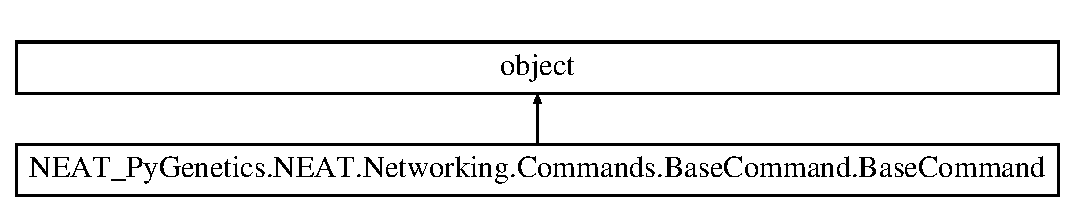
\includegraphics[height=2.000000cm]{classNEAT__PyGenetics_1_1NEAT_1_1Networking_1_1Commands_1_1BaseCommand_1_1BaseCommand}
\end{center}
\end{figure}
\subsection*{Public Member Functions}
\begin{DoxyCompactItemize}
\item 
def \hyperlink{classNEAT__PyGenetics_1_1NEAT_1_1Networking_1_1Commands_1_1BaseCommand_1_1BaseCommand_a7f060792cc1f8ea526bc47c592eae10e}{\+\_\+\+\_\+init\+\_\+\+\_\+} (self)
\item 
def \hyperlink{classNEAT__PyGenetics_1_1NEAT_1_1Networking_1_1Commands_1_1BaseCommand_1_1BaseCommand_a7466f3e151d869df0c0680aeaabd5497}{from\+\_\+dict} (self, dictionary)
\item 
def \hyperlink{classNEAT__PyGenetics_1_1NEAT_1_1Networking_1_1Commands_1_1BaseCommand_1_1BaseCommand_af8833907610ee782bbf991be49efe73f}{as\+\_\+dict} (self)
\item 
def \hyperlink{classNEAT__PyGenetics_1_1NEAT_1_1Networking_1_1Commands_1_1BaseCommand_1_1BaseCommand_a255f188c1306814a7840d33dfcf7650c}{acknowledged} (self)
\item 
def \hyperlink{classNEAT__PyGenetics_1_1NEAT_1_1Networking_1_1Commands_1_1BaseCommand_1_1BaseCommand_a631800c4e60223cee2fed6930a7b47df}{type} (self)
\item 
def \hyperlink{classNEAT__PyGenetics_1_1NEAT_1_1Networking_1_1Commands_1_1BaseCommand_1_1BaseCommand_ae1b33bc9a9dad6bcb9f2d3bb28c7355f}{\+\_\+\+\_\+eq\+\_\+\+\_\+}
\end{DoxyCompactItemize}
\subsection*{Public Attributes}
\begin{DoxyCompactItemize}
\item 
\hyperlink{classNEAT__PyGenetics_1_1NEAT_1_1Networking_1_1Commands_1_1BaseCommand_1_1BaseCommand_a50465fec7d23d12cfca6cd0d8b6b8a67}{parameters}
\item 
\hyperlink{classNEAT__PyGenetics_1_1NEAT_1_1Networking_1_1Commands_1_1BaseCommand_1_1BaseCommand_aa3136732344967769c806b465e699858}{result}
\end{DoxyCompactItemize}


\subsection{Constructor \& Destructor Documentation}
\index{N\+E\+A\+T\+\_\+\+Py\+Genetics\+::\+N\+E\+A\+T\+::\+Networking\+::\+Commands\+::\+Base\+Command\+::\+Base\+Command@{N\+E\+A\+T\+\_\+\+Py\+Genetics\+::\+N\+E\+A\+T\+::\+Networking\+::\+Commands\+::\+Base\+Command\+::\+Base\+Command}!\+\_\+\+\_\+init\+\_\+\+\_\+@{\+\_\+\+\_\+init\+\_\+\+\_\+}}
\index{\+\_\+\+\_\+init\+\_\+\+\_\+@{\+\_\+\+\_\+init\+\_\+\+\_\+}!N\+E\+A\+T\+\_\+\+Py\+Genetics\+::\+N\+E\+A\+T\+::\+Networking\+::\+Commands\+::\+Base\+Command\+::\+Base\+Command@{N\+E\+A\+T\+\_\+\+Py\+Genetics\+::\+N\+E\+A\+T\+::\+Networking\+::\+Commands\+::\+Base\+Command\+::\+Base\+Command}}
\subsubsection[{\texorpdfstring{\+\_\+\+\_\+init\+\_\+\+\_\+(self)}{__init__(self)}}]{\setlength{\rightskip}{0pt plus 5cm}def N\+E\+A\+T\+\_\+\+Py\+Genetics.\+N\+E\+A\+T.\+Networking.\+Commands.\+Base\+Command.\+Base\+Command.\+\_\+\+\_\+init\+\_\+\+\_\+ (
\begin{DoxyParamCaption}
\item[{}]{self}
\end{DoxyParamCaption}
)}\hypertarget{classNEAT__PyGenetics_1_1NEAT_1_1Networking_1_1Commands_1_1BaseCommand_1_1BaseCommand_a7f060792cc1f8ea526bc47c592eae10e}{}\label{classNEAT__PyGenetics_1_1NEAT_1_1Networking_1_1Commands_1_1BaseCommand_1_1BaseCommand_a7f060792cc1f8ea526bc47c592eae10e}


\subsection{Member Function Documentation}
\index{N\+E\+A\+T\+\_\+\+Py\+Genetics\+::\+N\+E\+A\+T\+::\+Networking\+::\+Commands\+::\+Base\+Command\+::\+Base\+Command@{N\+E\+A\+T\+\_\+\+Py\+Genetics\+::\+N\+E\+A\+T\+::\+Networking\+::\+Commands\+::\+Base\+Command\+::\+Base\+Command}!\+\_\+\+\_\+eq\+\_\+\+\_\+@{\+\_\+\+\_\+eq\+\_\+\+\_\+}}
\index{\+\_\+\+\_\+eq\+\_\+\+\_\+@{\+\_\+\+\_\+eq\+\_\+\+\_\+}!N\+E\+A\+T\+\_\+\+Py\+Genetics\+::\+N\+E\+A\+T\+::\+Networking\+::\+Commands\+::\+Base\+Command\+::\+Base\+Command@{N\+E\+A\+T\+\_\+\+Py\+Genetics\+::\+N\+E\+A\+T\+::\+Networking\+::\+Commands\+::\+Base\+Command\+::\+Base\+Command}}
\subsubsection[{\texorpdfstring{\+\_\+\+\_\+eq\+\_\+\+\_\+}{__eq__}}]{\setlength{\rightskip}{0pt plus 5cm}def N\+E\+A\+T\+\_\+\+Py\+Genetics.\+N\+E\+A\+T.\+Networking.\+Commands.\+Base\+Command.\+Base\+Command.\+\_\+\+\_\+eq\+\_\+\+\_\+ (
\begin{DoxyParamCaption}
\item[{}]{self, }
\item[{}]{obj}
\end{DoxyParamCaption}
)}\hypertarget{classNEAT__PyGenetics_1_1NEAT_1_1Networking_1_1Commands_1_1BaseCommand_1_1BaseCommand_ae1b33bc9a9dad6bcb9f2d3bb28c7355f}{}\label{classNEAT__PyGenetics_1_1NEAT_1_1Networking_1_1Commands_1_1BaseCommand_1_1BaseCommand_ae1b33bc9a9dad6bcb9f2d3bb28c7355f}
\index{N\+E\+A\+T\+\_\+\+Py\+Genetics\+::\+N\+E\+A\+T\+::\+Networking\+::\+Commands\+::\+Base\+Command\+::\+Base\+Command@{N\+E\+A\+T\+\_\+\+Py\+Genetics\+::\+N\+E\+A\+T\+::\+Networking\+::\+Commands\+::\+Base\+Command\+::\+Base\+Command}!acknowledged@{acknowledged}}
\index{acknowledged@{acknowledged}!N\+E\+A\+T\+\_\+\+Py\+Genetics\+::\+N\+E\+A\+T\+::\+Networking\+::\+Commands\+::\+Base\+Command\+::\+Base\+Command@{N\+E\+A\+T\+\_\+\+Py\+Genetics\+::\+N\+E\+A\+T\+::\+Networking\+::\+Commands\+::\+Base\+Command\+::\+Base\+Command}}
\subsubsection[{\texorpdfstring{acknowledged(self)}{acknowledged(self)}}]{\setlength{\rightskip}{0pt plus 5cm}def N\+E\+A\+T\+\_\+\+Py\+Genetics.\+N\+E\+A\+T.\+Networking.\+Commands.\+Base\+Command.\+Base\+Command.\+acknowledged (
\begin{DoxyParamCaption}
\item[{}]{self}
\end{DoxyParamCaption}
)}\hypertarget{classNEAT__PyGenetics_1_1NEAT_1_1Networking_1_1Commands_1_1BaseCommand_1_1BaseCommand_a255f188c1306814a7840d33dfcf7650c}{}\label{classNEAT__PyGenetics_1_1NEAT_1_1Networking_1_1Commands_1_1BaseCommand_1_1BaseCommand_a255f188c1306814a7840d33dfcf7650c}
\index{N\+E\+A\+T\+\_\+\+Py\+Genetics\+::\+N\+E\+A\+T\+::\+Networking\+::\+Commands\+::\+Base\+Command\+::\+Base\+Command@{N\+E\+A\+T\+\_\+\+Py\+Genetics\+::\+N\+E\+A\+T\+::\+Networking\+::\+Commands\+::\+Base\+Command\+::\+Base\+Command}!as\+\_\+dict@{as\+\_\+dict}}
\index{as\+\_\+dict@{as\+\_\+dict}!N\+E\+A\+T\+\_\+\+Py\+Genetics\+::\+N\+E\+A\+T\+::\+Networking\+::\+Commands\+::\+Base\+Command\+::\+Base\+Command@{N\+E\+A\+T\+\_\+\+Py\+Genetics\+::\+N\+E\+A\+T\+::\+Networking\+::\+Commands\+::\+Base\+Command\+::\+Base\+Command}}
\subsubsection[{\texorpdfstring{as\+\_\+dict(self)}{as_dict(self)}}]{\setlength{\rightskip}{0pt plus 5cm}def N\+E\+A\+T\+\_\+\+Py\+Genetics.\+N\+E\+A\+T.\+Networking.\+Commands.\+Base\+Command.\+Base\+Command.\+as\+\_\+dict (
\begin{DoxyParamCaption}
\item[{}]{self}
\end{DoxyParamCaption}
)}\hypertarget{classNEAT__PyGenetics_1_1NEAT_1_1Networking_1_1Commands_1_1BaseCommand_1_1BaseCommand_af8833907610ee782bbf991be49efe73f}{}\label{classNEAT__PyGenetics_1_1NEAT_1_1Networking_1_1Commands_1_1BaseCommand_1_1BaseCommand_af8833907610ee782bbf991be49efe73f}
\index{N\+E\+A\+T\+\_\+\+Py\+Genetics\+::\+N\+E\+A\+T\+::\+Networking\+::\+Commands\+::\+Base\+Command\+::\+Base\+Command@{N\+E\+A\+T\+\_\+\+Py\+Genetics\+::\+N\+E\+A\+T\+::\+Networking\+::\+Commands\+::\+Base\+Command\+::\+Base\+Command}!from\+\_\+dict@{from\+\_\+dict}}
\index{from\+\_\+dict@{from\+\_\+dict}!N\+E\+A\+T\+\_\+\+Py\+Genetics\+::\+N\+E\+A\+T\+::\+Networking\+::\+Commands\+::\+Base\+Command\+::\+Base\+Command@{N\+E\+A\+T\+\_\+\+Py\+Genetics\+::\+N\+E\+A\+T\+::\+Networking\+::\+Commands\+::\+Base\+Command\+::\+Base\+Command}}
\subsubsection[{\texorpdfstring{from\+\_\+dict(self, dictionary)}{from_dict(self, dictionary)}}]{\setlength{\rightskip}{0pt plus 5cm}def N\+E\+A\+T\+\_\+\+Py\+Genetics.\+N\+E\+A\+T.\+Networking.\+Commands.\+Base\+Command.\+Base\+Command.\+from\+\_\+dict (
\begin{DoxyParamCaption}
\item[{}]{self, }
\item[{}]{dictionary}
\end{DoxyParamCaption}
)}\hypertarget{classNEAT__PyGenetics_1_1NEAT_1_1Networking_1_1Commands_1_1BaseCommand_1_1BaseCommand_a7466f3e151d869df0c0680aeaabd5497}{}\label{classNEAT__PyGenetics_1_1NEAT_1_1Networking_1_1Commands_1_1BaseCommand_1_1BaseCommand_a7466f3e151d869df0c0680aeaabd5497}
\index{N\+E\+A\+T\+\_\+\+Py\+Genetics\+::\+N\+E\+A\+T\+::\+Networking\+::\+Commands\+::\+Base\+Command\+::\+Base\+Command@{N\+E\+A\+T\+\_\+\+Py\+Genetics\+::\+N\+E\+A\+T\+::\+Networking\+::\+Commands\+::\+Base\+Command\+::\+Base\+Command}!type@{type}}
\index{type@{type}!N\+E\+A\+T\+\_\+\+Py\+Genetics\+::\+N\+E\+A\+T\+::\+Networking\+::\+Commands\+::\+Base\+Command\+::\+Base\+Command@{N\+E\+A\+T\+\_\+\+Py\+Genetics\+::\+N\+E\+A\+T\+::\+Networking\+::\+Commands\+::\+Base\+Command\+::\+Base\+Command}}
\subsubsection[{\texorpdfstring{type(self)}{type(self)}}]{\setlength{\rightskip}{0pt plus 5cm}def N\+E\+A\+T\+\_\+\+Py\+Genetics.\+N\+E\+A\+T.\+Networking.\+Commands.\+Base\+Command.\+Base\+Command.\+type (
\begin{DoxyParamCaption}
\item[{}]{self}
\end{DoxyParamCaption}
)}\hypertarget{classNEAT__PyGenetics_1_1NEAT_1_1Networking_1_1Commands_1_1BaseCommand_1_1BaseCommand_a631800c4e60223cee2fed6930a7b47df}{}\label{classNEAT__PyGenetics_1_1NEAT_1_1Networking_1_1Commands_1_1BaseCommand_1_1BaseCommand_a631800c4e60223cee2fed6930a7b47df}


\subsection{Member Data Documentation}
\index{N\+E\+A\+T\+\_\+\+Py\+Genetics\+::\+N\+E\+A\+T\+::\+Networking\+::\+Commands\+::\+Base\+Command\+::\+Base\+Command@{N\+E\+A\+T\+\_\+\+Py\+Genetics\+::\+N\+E\+A\+T\+::\+Networking\+::\+Commands\+::\+Base\+Command\+::\+Base\+Command}!parameters@{parameters}}
\index{parameters@{parameters}!N\+E\+A\+T\+\_\+\+Py\+Genetics\+::\+N\+E\+A\+T\+::\+Networking\+::\+Commands\+::\+Base\+Command\+::\+Base\+Command@{N\+E\+A\+T\+\_\+\+Py\+Genetics\+::\+N\+E\+A\+T\+::\+Networking\+::\+Commands\+::\+Base\+Command\+::\+Base\+Command}}
\subsubsection[{\texorpdfstring{parameters}{parameters}}]{\setlength{\rightskip}{0pt plus 5cm}N\+E\+A\+T\+\_\+\+Py\+Genetics.\+N\+E\+A\+T.\+Networking.\+Commands.\+Base\+Command.\+Base\+Command.\+parameters}\hypertarget{classNEAT__PyGenetics_1_1NEAT_1_1Networking_1_1Commands_1_1BaseCommand_1_1BaseCommand_a50465fec7d23d12cfca6cd0d8b6b8a67}{}\label{classNEAT__PyGenetics_1_1NEAT_1_1Networking_1_1Commands_1_1BaseCommand_1_1BaseCommand_a50465fec7d23d12cfca6cd0d8b6b8a67}
\index{N\+E\+A\+T\+\_\+\+Py\+Genetics\+::\+N\+E\+A\+T\+::\+Networking\+::\+Commands\+::\+Base\+Command\+::\+Base\+Command@{N\+E\+A\+T\+\_\+\+Py\+Genetics\+::\+N\+E\+A\+T\+::\+Networking\+::\+Commands\+::\+Base\+Command\+::\+Base\+Command}!result@{result}}
\index{result@{result}!N\+E\+A\+T\+\_\+\+Py\+Genetics\+::\+N\+E\+A\+T\+::\+Networking\+::\+Commands\+::\+Base\+Command\+::\+Base\+Command@{N\+E\+A\+T\+\_\+\+Py\+Genetics\+::\+N\+E\+A\+T\+::\+Networking\+::\+Commands\+::\+Base\+Command\+::\+Base\+Command}}
\subsubsection[{\texorpdfstring{result}{result}}]{\setlength{\rightskip}{0pt plus 5cm}N\+E\+A\+T\+\_\+\+Py\+Genetics.\+N\+E\+A\+T.\+Networking.\+Commands.\+Base\+Command.\+Base\+Command.\+result}\hypertarget{classNEAT__PyGenetics_1_1NEAT_1_1Networking_1_1Commands_1_1BaseCommand_1_1BaseCommand_aa3136732344967769c806b465e699858}{}\label{classNEAT__PyGenetics_1_1NEAT_1_1Networking_1_1Commands_1_1BaseCommand_1_1BaseCommand_aa3136732344967769c806b465e699858}


The documentation for this class was generated from the following file\+:\begin{DoxyCompactItemize}
\item 
N\+E\+A\+T/\+Networking/\+Commands/\hyperlink{BaseCommand_8py}{Base\+Command.\+py}\end{DoxyCompactItemize}

\hypertarget{classNEAT__PyGenetics_1_1NEAT_1_1Generator_1_1Breeder_1_1Breeder}{}\section{N\+E\+A\+T\+\_\+\+Py\+Genetics.\+N\+E\+A\+T.\+Generator.\+Breeder.\+Breeder Class Reference}
\label{classNEAT__PyGenetics_1_1NEAT_1_1Generator_1_1Breeder_1_1Breeder}\index{N\+E\+A\+T\+\_\+\+Py\+Genetics.\+N\+E\+A\+T.\+Generator.\+Breeder.\+Breeder@{N\+E\+A\+T\+\_\+\+Py\+Genetics.\+N\+E\+A\+T.\+Generator.\+Breeder.\+Breeder}}
Inheritance diagram for N\+E\+A\+T\+\_\+\+Py\+Genetics.\+N\+E\+A\+T.\+Generator.\+Breeder.\+Breeder\+:\begin{figure}[H]
\begin{center}
\leavevmode
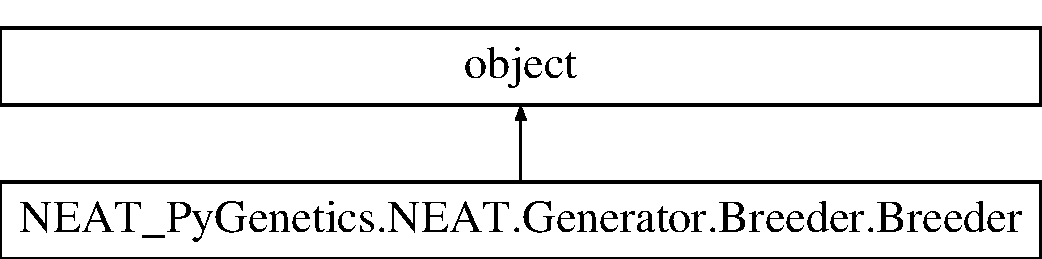
\includegraphics[height=2.000000cm]{classNEAT__PyGenetics_1_1NEAT_1_1Generator_1_1Breeder_1_1Breeder}
\end{center}
\end{figure}
\subsection*{Public Member Functions}
\begin{DoxyCompactItemize}
\item 
def \hyperlink{classNEAT__PyGenetics_1_1NEAT_1_1Generator_1_1Breeder_1_1Breeder_a99ffddd6afb3f995598605e165772515}{\+\_\+\+\_\+init\+\_\+\+\_\+}
\item 
def \hyperlink{classNEAT__PyGenetics_1_1NEAT_1_1Generator_1_1Breeder_1_1Breeder_a6e78ccec465831c858910b1319e75076}{breed\+\_\+genomes}
\begin{DoxyCompactList}\small\item\em Generates a new genome based on two input genomes. \end{DoxyCompactList}\item 
def \hyperlink{classNEAT__PyGenetics_1_1NEAT_1_1Generator_1_1Breeder_1_1Breeder_a761995541d6d9ff88e2ee112a57dff0f}{should\+\_\+gene\+\_\+be\+\_\+enabled} (self, instance\+\_\+one, instance\+\_\+two=None)
\begin{DoxyCompactList}\small\item\em Decides whether the inherited variant of a gene should be enabled in the offspring genome based on both parents\textquotesingle{} instances of the gene. \end{DoxyCompactList}\end{DoxyCompactItemize}
\subsection*{Static Public Attributes}
\begin{DoxyCompactItemize}
\item 
\hyperlink{classNEAT__PyGenetics_1_1NEAT_1_1Generator_1_1Breeder_1_1Breeder_a0e28efbae8c7fdce0a0c0f1b7c7abe02}{breeding\+\_\+parameters}
\item 
\hyperlink{classNEAT__PyGenetics_1_1NEAT_1_1Generator_1_1Breeder_1_1Breeder_a4b2204333e2b891725b9d7eac0f9533b}{bigger\+\_\+genome}
\item 
\hyperlink{classNEAT__PyGenetics_1_1NEAT_1_1Generator_1_1Breeder_1_1Breeder_aee42ab257302cbcf2e6619111289c489}{smaller\+\_\+genome}
\item 
\hyperlink{classNEAT__PyGenetics_1_1NEAT_1_1Generator_1_1Breeder_1_1Breeder_aae86e270174a1ddc14677a5bd267ceda}{bigger\+\_\+genome\+\_\+gene\+\_\+ids}
\item 
\hyperlink{classNEAT__PyGenetics_1_1NEAT_1_1Generator_1_1Breeder_1_1Breeder_a1b7a43f5e5d325a0581e90e5666cc424}{smaller\+\_\+genome\+\_\+gene\+\_\+ids}
\item 
\hyperlink{classNEAT__PyGenetics_1_1NEAT_1_1Generator_1_1Breeder_1_1Breeder_aafd044323f51754e3d3ed1c56398b88b}{all\+\_\+gene\+\_\+ids}
\item 
\hyperlink{classNEAT__PyGenetics_1_1NEAT_1_1Generator_1_1Breeder_1_1Breeder_a017b63dcfc04f983f3097f52d1b2ba80}{matching\+\_\+gene\+\_\+ids}
\item 
\hyperlink{classNEAT__PyGenetics_1_1NEAT_1_1Generator_1_1Breeder_1_1Breeder_a3ef5f23263b2205639606d0c9756e79c}{differing\+\_\+gene\+\_\+ids}
\item 
\hyperlink{classNEAT__PyGenetics_1_1NEAT_1_1Generator_1_1Breeder_1_1Breeder_a6898cc6d6a36379227d5a00f9e627432}{fitter\+\_\+genome\+\_\+table}
\item 
\hyperlink{classNEAT__PyGenetics_1_1NEAT_1_1Generator_1_1Breeder_1_1Breeder_a8ecfda7d3fcfc166577e07cc977fa9cb}{new\+\_\+genome}
\item 
\hyperlink{classNEAT__PyGenetics_1_1NEAT_1_1Generator_1_1Breeder_1_1Breeder_a57dfe8e0f1eff1f6ef84492bc845dd40}{parent\+\_\+genome\+\_\+table}
\item 
\hyperlink{classNEAT__PyGenetics_1_1NEAT_1_1Generator_1_1Breeder_1_1Breeder_a11f9b1f5d4b9804dd8b54db956734938}{gene\+\_\+enabled}
\item 
\hyperlink{classNEAT__PyGenetics_1_1NEAT_1_1Generator_1_1Breeder_1_1Breeder_a1e14b916370fa769ae820893190a1f28}{gene\+\_\+weight}
\item 
\hyperlink{classNEAT__PyGenetics_1_1NEAT_1_1Generator_1_1Breeder_1_1Breeder_a82bb0cf6761460a4478abd22fc41e256}{inherit\+\_\+gene}
\end{DoxyCompactItemize}


\subsection{Constructor \& Destructor Documentation}
\index{N\+E\+A\+T\+\_\+\+Py\+Genetics\+::\+N\+E\+A\+T\+::\+Generator\+::\+Breeder\+::\+Breeder@{N\+E\+A\+T\+\_\+\+Py\+Genetics\+::\+N\+E\+A\+T\+::\+Generator\+::\+Breeder\+::\+Breeder}!\+\_\+\+\_\+init\+\_\+\+\_\+@{\+\_\+\+\_\+init\+\_\+\+\_\+}}
\index{\+\_\+\+\_\+init\+\_\+\+\_\+@{\+\_\+\+\_\+init\+\_\+\+\_\+}!N\+E\+A\+T\+\_\+\+Py\+Genetics\+::\+N\+E\+A\+T\+::\+Generator\+::\+Breeder\+::\+Breeder@{N\+E\+A\+T\+\_\+\+Py\+Genetics\+::\+N\+E\+A\+T\+::\+Generator\+::\+Breeder\+::\+Breeder}}
\subsubsection[{\texorpdfstring{\+\_\+\+\_\+init\+\_\+\+\_\+}{__init__}}]{\setlength{\rightskip}{0pt plus 5cm}def N\+E\+A\+T\+\_\+\+Py\+Genetics.\+N\+E\+A\+T.\+Generator.\+Breeder.\+Breeder.\+\_\+\+\_\+init\+\_\+\+\_\+ (
\begin{DoxyParamCaption}
\item[{}]{self, }
\item[{}]{breeding\+\_\+parameters}
\end{DoxyParamCaption}
)}\hypertarget{classNEAT__PyGenetics_1_1NEAT_1_1Generator_1_1Breeder_1_1Breeder_a99ffddd6afb3f995598605e165772515}{}\label{classNEAT__PyGenetics_1_1NEAT_1_1Generator_1_1Breeder_1_1Breeder_a99ffddd6afb3f995598605e165772515}


\subsection{Member Function Documentation}
\index{N\+E\+A\+T\+\_\+\+Py\+Genetics\+::\+N\+E\+A\+T\+::\+Generator\+::\+Breeder\+::\+Breeder@{N\+E\+A\+T\+\_\+\+Py\+Genetics\+::\+N\+E\+A\+T\+::\+Generator\+::\+Breeder\+::\+Breeder}!breed\+\_\+genomes@{breed\+\_\+genomes}}
\index{breed\+\_\+genomes@{breed\+\_\+genomes}!N\+E\+A\+T\+\_\+\+Py\+Genetics\+::\+N\+E\+A\+T\+::\+Generator\+::\+Breeder\+::\+Breeder@{N\+E\+A\+T\+\_\+\+Py\+Genetics\+::\+N\+E\+A\+T\+::\+Generator\+::\+Breeder\+::\+Breeder}}
\subsubsection[{\texorpdfstring{breed\+\_\+genomes}{breed_genomes}}]{\setlength{\rightskip}{0pt plus 5cm}def N\+E\+A\+T\+\_\+\+Py\+Genetics.\+N\+E\+A\+T.\+Generator.\+Breeder.\+Breeder.\+breed\+\_\+genomes (
\begin{DoxyParamCaption}
\item[{}]{self, }
\item[{}]{genome\+\_\+one}
\end{DoxyParamCaption}
)}\hypertarget{classNEAT__PyGenetics_1_1NEAT_1_1Generator_1_1Breeder_1_1Breeder_a6e78ccec465831c858910b1319e75076}{}\label{classNEAT__PyGenetics_1_1NEAT_1_1Generator_1_1Breeder_1_1Breeder_a6e78ccec465831c858910b1319e75076}


Generates a new genome based on two input genomes. 

Matching genes are inherited randomly from one of the parents. Differing genes are inherited from the fitter parent. If the fitness value difference is below fitness\+\_\+difference\+\_\+threshold, the differing genes are inherited randomly as well.

\+:param genome\+\_\+one\+: \+:param genome\+\_\+two\+: \+:return\+: \index{N\+E\+A\+T\+\_\+\+Py\+Genetics\+::\+N\+E\+A\+T\+::\+Generator\+::\+Breeder\+::\+Breeder@{N\+E\+A\+T\+\_\+\+Py\+Genetics\+::\+N\+E\+A\+T\+::\+Generator\+::\+Breeder\+::\+Breeder}!should\+\_\+gene\+\_\+be\+\_\+enabled@{should\+\_\+gene\+\_\+be\+\_\+enabled}}
\index{should\+\_\+gene\+\_\+be\+\_\+enabled@{should\+\_\+gene\+\_\+be\+\_\+enabled}!N\+E\+A\+T\+\_\+\+Py\+Genetics\+::\+N\+E\+A\+T\+::\+Generator\+::\+Breeder\+::\+Breeder@{N\+E\+A\+T\+\_\+\+Py\+Genetics\+::\+N\+E\+A\+T\+::\+Generator\+::\+Breeder\+::\+Breeder}}
\subsubsection[{\texorpdfstring{should\+\_\+gene\+\_\+be\+\_\+enabled(self, instance\+\_\+one, instance\+\_\+two=\+None)}{should_gene_be_enabled(self, instance_one, instance_two=None)}}]{\setlength{\rightskip}{0pt plus 5cm}def N\+E\+A\+T\+\_\+\+Py\+Genetics.\+N\+E\+A\+T.\+Generator.\+Breeder.\+Breeder.\+should\+\_\+gene\+\_\+be\+\_\+enabled (
\begin{DoxyParamCaption}
\item[{}]{self, }
\item[{}]{instance\+\_\+one, }
\item[{}]{instance\+\_\+two = {\ttfamily None}}
\end{DoxyParamCaption}
)}\hypertarget{classNEAT__PyGenetics_1_1NEAT_1_1Generator_1_1Breeder_1_1Breeder_a761995541d6d9ff88e2ee112a57dff0f}{}\label{classNEAT__PyGenetics_1_1NEAT_1_1Generator_1_1Breeder_1_1Breeder_a761995541d6d9ff88e2ee112a57dff0f}


Decides whether the inherited variant of a gene should be enabled in the offspring genome based on both parents\textquotesingle{} instances of the gene. 

\+:param instance\+\_\+one\+: The first gene instance \+:param instance\+\_\+two\+: The second gene instance \+:return\+: Whether the inherited gene should be enabled 

\subsection{Member Data Documentation}
\index{N\+E\+A\+T\+\_\+\+Py\+Genetics\+::\+N\+E\+A\+T\+::\+Generator\+::\+Breeder\+::\+Breeder@{N\+E\+A\+T\+\_\+\+Py\+Genetics\+::\+N\+E\+A\+T\+::\+Generator\+::\+Breeder\+::\+Breeder}!all\+\_\+gene\+\_\+ids@{all\+\_\+gene\+\_\+ids}}
\index{all\+\_\+gene\+\_\+ids@{all\+\_\+gene\+\_\+ids}!N\+E\+A\+T\+\_\+\+Py\+Genetics\+::\+N\+E\+A\+T\+::\+Generator\+::\+Breeder\+::\+Breeder@{N\+E\+A\+T\+\_\+\+Py\+Genetics\+::\+N\+E\+A\+T\+::\+Generator\+::\+Breeder\+::\+Breeder}}
\subsubsection[{\texorpdfstring{all\+\_\+gene\+\_\+ids}{all_gene_ids}}]{\setlength{\rightskip}{0pt plus 5cm}N\+E\+A\+T\+\_\+\+Py\+Genetics.\+N\+E\+A\+T.\+Generator.\+Breeder.\+Breeder.\+all\+\_\+gene\+\_\+ids\hspace{0.3cm}{\ttfamily [static]}}\hypertarget{classNEAT__PyGenetics_1_1NEAT_1_1Generator_1_1Breeder_1_1Breeder_aafd044323f51754e3d3ed1c56398b88b}{}\label{classNEAT__PyGenetics_1_1NEAT_1_1Generator_1_1Breeder_1_1Breeder_aafd044323f51754e3d3ed1c56398b88b}
\index{N\+E\+A\+T\+\_\+\+Py\+Genetics\+::\+N\+E\+A\+T\+::\+Generator\+::\+Breeder\+::\+Breeder@{N\+E\+A\+T\+\_\+\+Py\+Genetics\+::\+N\+E\+A\+T\+::\+Generator\+::\+Breeder\+::\+Breeder}!bigger\+\_\+genome@{bigger\+\_\+genome}}
\index{bigger\+\_\+genome@{bigger\+\_\+genome}!N\+E\+A\+T\+\_\+\+Py\+Genetics\+::\+N\+E\+A\+T\+::\+Generator\+::\+Breeder\+::\+Breeder@{N\+E\+A\+T\+\_\+\+Py\+Genetics\+::\+N\+E\+A\+T\+::\+Generator\+::\+Breeder\+::\+Breeder}}
\subsubsection[{\texorpdfstring{bigger\+\_\+genome}{bigger_genome}}]{\setlength{\rightskip}{0pt plus 5cm}N\+E\+A\+T\+\_\+\+Py\+Genetics.\+N\+E\+A\+T.\+Generator.\+Breeder.\+Breeder.\+bigger\+\_\+genome\hspace{0.3cm}{\ttfamily [static]}}\hypertarget{classNEAT__PyGenetics_1_1NEAT_1_1Generator_1_1Breeder_1_1Breeder_a4b2204333e2b891725b9d7eac0f9533b}{}\label{classNEAT__PyGenetics_1_1NEAT_1_1Generator_1_1Breeder_1_1Breeder_a4b2204333e2b891725b9d7eac0f9533b}
\index{N\+E\+A\+T\+\_\+\+Py\+Genetics\+::\+N\+E\+A\+T\+::\+Generator\+::\+Breeder\+::\+Breeder@{N\+E\+A\+T\+\_\+\+Py\+Genetics\+::\+N\+E\+A\+T\+::\+Generator\+::\+Breeder\+::\+Breeder}!bigger\+\_\+genome\+\_\+gene\+\_\+ids@{bigger\+\_\+genome\+\_\+gene\+\_\+ids}}
\index{bigger\+\_\+genome\+\_\+gene\+\_\+ids@{bigger\+\_\+genome\+\_\+gene\+\_\+ids}!N\+E\+A\+T\+\_\+\+Py\+Genetics\+::\+N\+E\+A\+T\+::\+Generator\+::\+Breeder\+::\+Breeder@{N\+E\+A\+T\+\_\+\+Py\+Genetics\+::\+N\+E\+A\+T\+::\+Generator\+::\+Breeder\+::\+Breeder}}
\subsubsection[{\texorpdfstring{bigger\+\_\+genome\+\_\+gene\+\_\+ids}{bigger_genome_gene_ids}}]{\setlength{\rightskip}{0pt plus 5cm}N\+E\+A\+T\+\_\+\+Py\+Genetics.\+N\+E\+A\+T.\+Generator.\+Breeder.\+Breeder.\+bigger\+\_\+genome\+\_\+gene\+\_\+ids\hspace{0.3cm}{\ttfamily [static]}}\hypertarget{classNEAT__PyGenetics_1_1NEAT_1_1Generator_1_1Breeder_1_1Breeder_aae86e270174a1ddc14677a5bd267ceda}{}\label{classNEAT__PyGenetics_1_1NEAT_1_1Generator_1_1Breeder_1_1Breeder_aae86e270174a1ddc14677a5bd267ceda}
\index{N\+E\+A\+T\+\_\+\+Py\+Genetics\+::\+N\+E\+A\+T\+::\+Generator\+::\+Breeder\+::\+Breeder@{N\+E\+A\+T\+\_\+\+Py\+Genetics\+::\+N\+E\+A\+T\+::\+Generator\+::\+Breeder\+::\+Breeder}!breeding\+\_\+parameters@{breeding\+\_\+parameters}}
\index{breeding\+\_\+parameters@{breeding\+\_\+parameters}!N\+E\+A\+T\+\_\+\+Py\+Genetics\+::\+N\+E\+A\+T\+::\+Generator\+::\+Breeder\+::\+Breeder@{N\+E\+A\+T\+\_\+\+Py\+Genetics\+::\+N\+E\+A\+T\+::\+Generator\+::\+Breeder\+::\+Breeder}}
\subsubsection[{\texorpdfstring{breeding\+\_\+parameters}{breeding_parameters}}]{\setlength{\rightskip}{0pt plus 5cm}N\+E\+A\+T\+\_\+\+Py\+Genetics.\+N\+E\+A\+T.\+Generator.\+Breeder.\+Breeder.\+breeding\+\_\+parameters\hspace{0.3cm}{\ttfamily [static]}}\hypertarget{classNEAT__PyGenetics_1_1NEAT_1_1Generator_1_1Breeder_1_1Breeder_a0e28efbae8c7fdce0a0c0f1b7c7abe02}{}\label{classNEAT__PyGenetics_1_1NEAT_1_1Generator_1_1Breeder_1_1Breeder_a0e28efbae8c7fdce0a0c0f1b7c7abe02}
\index{N\+E\+A\+T\+\_\+\+Py\+Genetics\+::\+N\+E\+A\+T\+::\+Generator\+::\+Breeder\+::\+Breeder@{N\+E\+A\+T\+\_\+\+Py\+Genetics\+::\+N\+E\+A\+T\+::\+Generator\+::\+Breeder\+::\+Breeder}!differing\+\_\+gene\+\_\+ids@{differing\+\_\+gene\+\_\+ids}}
\index{differing\+\_\+gene\+\_\+ids@{differing\+\_\+gene\+\_\+ids}!N\+E\+A\+T\+\_\+\+Py\+Genetics\+::\+N\+E\+A\+T\+::\+Generator\+::\+Breeder\+::\+Breeder@{N\+E\+A\+T\+\_\+\+Py\+Genetics\+::\+N\+E\+A\+T\+::\+Generator\+::\+Breeder\+::\+Breeder}}
\subsubsection[{\texorpdfstring{differing\+\_\+gene\+\_\+ids}{differing_gene_ids}}]{\setlength{\rightskip}{0pt plus 5cm}N\+E\+A\+T\+\_\+\+Py\+Genetics.\+N\+E\+A\+T.\+Generator.\+Breeder.\+Breeder.\+differing\+\_\+gene\+\_\+ids\hspace{0.3cm}{\ttfamily [static]}}\hypertarget{classNEAT__PyGenetics_1_1NEAT_1_1Generator_1_1Breeder_1_1Breeder_a3ef5f23263b2205639606d0c9756e79c}{}\label{classNEAT__PyGenetics_1_1NEAT_1_1Generator_1_1Breeder_1_1Breeder_a3ef5f23263b2205639606d0c9756e79c}
\index{N\+E\+A\+T\+\_\+\+Py\+Genetics\+::\+N\+E\+A\+T\+::\+Generator\+::\+Breeder\+::\+Breeder@{N\+E\+A\+T\+\_\+\+Py\+Genetics\+::\+N\+E\+A\+T\+::\+Generator\+::\+Breeder\+::\+Breeder}!fitter\+\_\+genome\+\_\+table@{fitter\+\_\+genome\+\_\+table}}
\index{fitter\+\_\+genome\+\_\+table@{fitter\+\_\+genome\+\_\+table}!N\+E\+A\+T\+\_\+\+Py\+Genetics\+::\+N\+E\+A\+T\+::\+Generator\+::\+Breeder\+::\+Breeder@{N\+E\+A\+T\+\_\+\+Py\+Genetics\+::\+N\+E\+A\+T\+::\+Generator\+::\+Breeder\+::\+Breeder}}
\subsubsection[{\texorpdfstring{fitter\+\_\+genome\+\_\+table}{fitter_genome_table}}]{\setlength{\rightskip}{0pt plus 5cm}N\+E\+A\+T\+\_\+\+Py\+Genetics.\+N\+E\+A\+T.\+Generator.\+Breeder.\+Breeder.\+fitter\+\_\+genome\+\_\+table\hspace{0.3cm}{\ttfamily [static]}}\hypertarget{classNEAT__PyGenetics_1_1NEAT_1_1Generator_1_1Breeder_1_1Breeder_a6898cc6d6a36379227d5a00f9e627432}{}\label{classNEAT__PyGenetics_1_1NEAT_1_1Generator_1_1Breeder_1_1Breeder_a6898cc6d6a36379227d5a00f9e627432}
\index{N\+E\+A\+T\+\_\+\+Py\+Genetics\+::\+N\+E\+A\+T\+::\+Generator\+::\+Breeder\+::\+Breeder@{N\+E\+A\+T\+\_\+\+Py\+Genetics\+::\+N\+E\+A\+T\+::\+Generator\+::\+Breeder\+::\+Breeder}!gene\+\_\+enabled@{gene\+\_\+enabled}}
\index{gene\+\_\+enabled@{gene\+\_\+enabled}!N\+E\+A\+T\+\_\+\+Py\+Genetics\+::\+N\+E\+A\+T\+::\+Generator\+::\+Breeder\+::\+Breeder@{N\+E\+A\+T\+\_\+\+Py\+Genetics\+::\+N\+E\+A\+T\+::\+Generator\+::\+Breeder\+::\+Breeder}}
\subsubsection[{\texorpdfstring{gene\+\_\+enabled}{gene_enabled}}]{\setlength{\rightskip}{0pt plus 5cm}N\+E\+A\+T\+\_\+\+Py\+Genetics.\+N\+E\+A\+T.\+Generator.\+Breeder.\+Breeder.\+gene\+\_\+enabled\hspace{0.3cm}{\ttfamily [static]}}\hypertarget{classNEAT__PyGenetics_1_1NEAT_1_1Generator_1_1Breeder_1_1Breeder_a11f9b1f5d4b9804dd8b54db956734938}{}\label{classNEAT__PyGenetics_1_1NEAT_1_1Generator_1_1Breeder_1_1Breeder_a11f9b1f5d4b9804dd8b54db956734938}
\index{N\+E\+A\+T\+\_\+\+Py\+Genetics\+::\+N\+E\+A\+T\+::\+Generator\+::\+Breeder\+::\+Breeder@{N\+E\+A\+T\+\_\+\+Py\+Genetics\+::\+N\+E\+A\+T\+::\+Generator\+::\+Breeder\+::\+Breeder}!gene\+\_\+weight@{gene\+\_\+weight}}
\index{gene\+\_\+weight@{gene\+\_\+weight}!N\+E\+A\+T\+\_\+\+Py\+Genetics\+::\+N\+E\+A\+T\+::\+Generator\+::\+Breeder\+::\+Breeder@{N\+E\+A\+T\+\_\+\+Py\+Genetics\+::\+N\+E\+A\+T\+::\+Generator\+::\+Breeder\+::\+Breeder}}
\subsubsection[{\texorpdfstring{gene\+\_\+weight}{gene_weight}}]{\setlength{\rightskip}{0pt plus 5cm}N\+E\+A\+T\+\_\+\+Py\+Genetics.\+N\+E\+A\+T.\+Generator.\+Breeder.\+Breeder.\+gene\+\_\+weight\hspace{0.3cm}{\ttfamily [static]}}\hypertarget{classNEAT__PyGenetics_1_1NEAT_1_1Generator_1_1Breeder_1_1Breeder_a1e14b916370fa769ae820893190a1f28}{}\label{classNEAT__PyGenetics_1_1NEAT_1_1Generator_1_1Breeder_1_1Breeder_a1e14b916370fa769ae820893190a1f28}
\index{N\+E\+A\+T\+\_\+\+Py\+Genetics\+::\+N\+E\+A\+T\+::\+Generator\+::\+Breeder\+::\+Breeder@{N\+E\+A\+T\+\_\+\+Py\+Genetics\+::\+N\+E\+A\+T\+::\+Generator\+::\+Breeder\+::\+Breeder}!inherit\+\_\+gene@{inherit\+\_\+gene}}
\index{inherit\+\_\+gene@{inherit\+\_\+gene}!N\+E\+A\+T\+\_\+\+Py\+Genetics\+::\+N\+E\+A\+T\+::\+Generator\+::\+Breeder\+::\+Breeder@{N\+E\+A\+T\+\_\+\+Py\+Genetics\+::\+N\+E\+A\+T\+::\+Generator\+::\+Breeder\+::\+Breeder}}
\subsubsection[{\texorpdfstring{inherit\+\_\+gene}{inherit_gene}}]{\setlength{\rightskip}{0pt plus 5cm}N\+E\+A\+T\+\_\+\+Py\+Genetics.\+N\+E\+A\+T.\+Generator.\+Breeder.\+Breeder.\+inherit\+\_\+gene\hspace{0.3cm}{\ttfamily [static]}}\hypertarget{classNEAT__PyGenetics_1_1NEAT_1_1Generator_1_1Breeder_1_1Breeder_a82bb0cf6761460a4478abd22fc41e256}{}\label{classNEAT__PyGenetics_1_1NEAT_1_1Generator_1_1Breeder_1_1Breeder_a82bb0cf6761460a4478abd22fc41e256}
\index{N\+E\+A\+T\+\_\+\+Py\+Genetics\+::\+N\+E\+A\+T\+::\+Generator\+::\+Breeder\+::\+Breeder@{N\+E\+A\+T\+\_\+\+Py\+Genetics\+::\+N\+E\+A\+T\+::\+Generator\+::\+Breeder\+::\+Breeder}!matching\+\_\+gene\+\_\+ids@{matching\+\_\+gene\+\_\+ids}}
\index{matching\+\_\+gene\+\_\+ids@{matching\+\_\+gene\+\_\+ids}!N\+E\+A\+T\+\_\+\+Py\+Genetics\+::\+N\+E\+A\+T\+::\+Generator\+::\+Breeder\+::\+Breeder@{N\+E\+A\+T\+\_\+\+Py\+Genetics\+::\+N\+E\+A\+T\+::\+Generator\+::\+Breeder\+::\+Breeder}}
\subsubsection[{\texorpdfstring{matching\+\_\+gene\+\_\+ids}{matching_gene_ids}}]{\setlength{\rightskip}{0pt plus 5cm}N\+E\+A\+T\+\_\+\+Py\+Genetics.\+N\+E\+A\+T.\+Generator.\+Breeder.\+Breeder.\+matching\+\_\+gene\+\_\+ids\hspace{0.3cm}{\ttfamily [static]}}\hypertarget{classNEAT__PyGenetics_1_1NEAT_1_1Generator_1_1Breeder_1_1Breeder_a017b63dcfc04f983f3097f52d1b2ba80}{}\label{classNEAT__PyGenetics_1_1NEAT_1_1Generator_1_1Breeder_1_1Breeder_a017b63dcfc04f983f3097f52d1b2ba80}
\index{N\+E\+A\+T\+\_\+\+Py\+Genetics\+::\+N\+E\+A\+T\+::\+Generator\+::\+Breeder\+::\+Breeder@{N\+E\+A\+T\+\_\+\+Py\+Genetics\+::\+N\+E\+A\+T\+::\+Generator\+::\+Breeder\+::\+Breeder}!new\+\_\+genome@{new\+\_\+genome}}
\index{new\+\_\+genome@{new\+\_\+genome}!N\+E\+A\+T\+\_\+\+Py\+Genetics\+::\+N\+E\+A\+T\+::\+Generator\+::\+Breeder\+::\+Breeder@{N\+E\+A\+T\+\_\+\+Py\+Genetics\+::\+N\+E\+A\+T\+::\+Generator\+::\+Breeder\+::\+Breeder}}
\subsubsection[{\texorpdfstring{new\+\_\+genome}{new_genome}}]{\setlength{\rightskip}{0pt plus 5cm}N\+E\+A\+T\+\_\+\+Py\+Genetics.\+N\+E\+A\+T.\+Generator.\+Breeder.\+Breeder.\+new\+\_\+genome\hspace{0.3cm}{\ttfamily [static]}}\hypertarget{classNEAT__PyGenetics_1_1NEAT_1_1Generator_1_1Breeder_1_1Breeder_a8ecfda7d3fcfc166577e07cc977fa9cb}{}\label{classNEAT__PyGenetics_1_1NEAT_1_1Generator_1_1Breeder_1_1Breeder_a8ecfda7d3fcfc166577e07cc977fa9cb}
\index{N\+E\+A\+T\+\_\+\+Py\+Genetics\+::\+N\+E\+A\+T\+::\+Generator\+::\+Breeder\+::\+Breeder@{N\+E\+A\+T\+\_\+\+Py\+Genetics\+::\+N\+E\+A\+T\+::\+Generator\+::\+Breeder\+::\+Breeder}!parent\+\_\+genome\+\_\+table@{parent\+\_\+genome\+\_\+table}}
\index{parent\+\_\+genome\+\_\+table@{parent\+\_\+genome\+\_\+table}!N\+E\+A\+T\+\_\+\+Py\+Genetics\+::\+N\+E\+A\+T\+::\+Generator\+::\+Breeder\+::\+Breeder@{N\+E\+A\+T\+\_\+\+Py\+Genetics\+::\+N\+E\+A\+T\+::\+Generator\+::\+Breeder\+::\+Breeder}}
\subsubsection[{\texorpdfstring{parent\+\_\+genome\+\_\+table}{parent_genome_table}}]{\setlength{\rightskip}{0pt plus 5cm}N\+E\+A\+T\+\_\+\+Py\+Genetics.\+N\+E\+A\+T.\+Generator.\+Breeder.\+Breeder.\+parent\+\_\+genome\+\_\+table\hspace{0.3cm}{\ttfamily [static]}}\hypertarget{classNEAT__PyGenetics_1_1NEAT_1_1Generator_1_1Breeder_1_1Breeder_a57dfe8e0f1eff1f6ef84492bc845dd40}{}\label{classNEAT__PyGenetics_1_1NEAT_1_1Generator_1_1Breeder_1_1Breeder_a57dfe8e0f1eff1f6ef84492bc845dd40}
\index{N\+E\+A\+T\+\_\+\+Py\+Genetics\+::\+N\+E\+A\+T\+::\+Generator\+::\+Breeder\+::\+Breeder@{N\+E\+A\+T\+\_\+\+Py\+Genetics\+::\+N\+E\+A\+T\+::\+Generator\+::\+Breeder\+::\+Breeder}!smaller\+\_\+genome@{smaller\+\_\+genome}}
\index{smaller\+\_\+genome@{smaller\+\_\+genome}!N\+E\+A\+T\+\_\+\+Py\+Genetics\+::\+N\+E\+A\+T\+::\+Generator\+::\+Breeder\+::\+Breeder@{N\+E\+A\+T\+\_\+\+Py\+Genetics\+::\+N\+E\+A\+T\+::\+Generator\+::\+Breeder\+::\+Breeder}}
\subsubsection[{\texorpdfstring{smaller\+\_\+genome}{smaller_genome}}]{\setlength{\rightskip}{0pt plus 5cm}N\+E\+A\+T\+\_\+\+Py\+Genetics.\+N\+E\+A\+T.\+Generator.\+Breeder.\+Breeder.\+smaller\+\_\+genome\hspace{0.3cm}{\ttfamily [static]}}\hypertarget{classNEAT__PyGenetics_1_1NEAT_1_1Generator_1_1Breeder_1_1Breeder_aee42ab257302cbcf2e6619111289c489}{}\label{classNEAT__PyGenetics_1_1NEAT_1_1Generator_1_1Breeder_1_1Breeder_aee42ab257302cbcf2e6619111289c489}
\index{N\+E\+A\+T\+\_\+\+Py\+Genetics\+::\+N\+E\+A\+T\+::\+Generator\+::\+Breeder\+::\+Breeder@{N\+E\+A\+T\+\_\+\+Py\+Genetics\+::\+N\+E\+A\+T\+::\+Generator\+::\+Breeder\+::\+Breeder}!smaller\+\_\+genome\+\_\+gene\+\_\+ids@{smaller\+\_\+genome\+\_\+gene\+\_\+ids}}
\index{smaller\+\_\+genome\+\_\+gene\+\_\+ids@{smaller\+\_\+genome\+\_\+gene\+\_\+ids}!N\+E\+A\+T\+\_\+\+Py\+Genetics\+::\+N\+E\+A\+T\+::\+Generator\+::\+Breeder\+::\+Breeder@{N\+E\+A\+T\+\_\+\+Py\+Genetics\+::\+N\+E\+A\+T\+::\+Generator\+::\+Breeder\+::\+Breeder}}
\subsubsection[{\texorpdfstring{smaller\+\_\+genome\+\_\+gene\+\_\+ids}{smaller_genome_gene_ids}}]{\setlength{\rightskip}{0pt plus 5cm}N\+E\+A\+T\+\_\+\+Py\+Genetics.\+N\+E\+A\+T.\+Generator.\+Breeder.\+Breeder.\+smaller\+\_\+genome\+\_\+gene\+\_\+ids\hspace{0.3cm}{\ttfamily [static]}}\hypertarget{classNEAT__PyGenetics_1_1NEAT_1_1Generator_1_1Breeder_1_1Breeder_a1b7a43f5e5d325a0581e90e5666cc424}{}\label{classNEAT__PyGenetics_1_1NEAT_1_1Generator_1_1Breeder_1_1Breeder_a1b7a43f5e5d325a0581e90e5666cc424}


The documentation for this class was generated from the following file\+:\begin{DoxyCompactItemize}
\item 
N\+E\+A\+T/\+Generator/\hyperlink{Breeder_8py}{Breeder.\+py}\end{DoxyCompactItemize}

\hypertarget{classNEAT__PyGenetics_1_1NEAT_1_1Analyst_1_1Cluster_1_1Cluster}{}\section{N\+E\+A\+T\+\_\+\+Py\+Genetics.\+N\+E\+A\+T.\+Analyst.\+Cluster.\+Cluster Class Reference}
\label{classNEAT__PyGenetics_1_1NEAT_1_1Analyst_1_1Cluster_1_1Cluster}\index{N\+E\+A\+T\+\_\+\+Py\+Genetics.\+N\+E\+A\+T.\+Analyst.\+Cluster.\+Cluster@{N\+E\+A\+T\+\_\+\+Py\+Genetics.\+N\+E\+A\+T.\+Analyst.\+Cluster.\+Cluster}}
Inheritance diagram for N\+E\+A\+T\+\_\+\+Py\+Genetics.\+N\+E\+A\+T.\+Analyst.\+Cluster.\+Cluster\+:\begin{figure}[H]
\begin{center}
\leavevmode
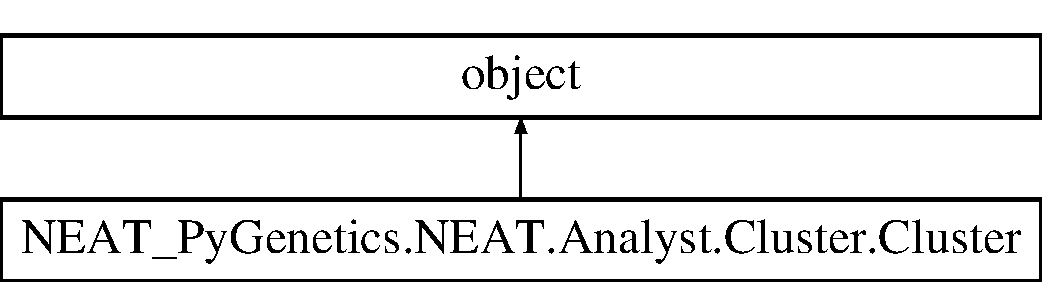
\includegraphics[height=2.000000cm]{classNEAT__PyGenetics_1_1NEAT_1_1Analyst_1_1Cluster_1_1Cluster}
\end{center}
\end{figure}
\subsection*{Public Member Functions}
\begin{DoxyCompactItemize}
\item 
def \hyperlink{classNEAT__PyGenetics_1_1NEAT_1_1Analyst_1_1Cluster_1_1Cluster_a12ebc01de1535941e1af477dddaedbe9}{\+\_\+\+\_\+init\+\_\+\+\_\+} (self)
\item 
def \hyperlink{classNEAT__PyGenetics_1_1NEAT_1_1Analyst_1_1Cluster_1_1Cluster_a85d2dfa24ff6846be17920a77987ece5}{\+\_\+\+\_\+eq\+\_\+\+\_\+}
\item 
def \hyperlink{classNEAT__PyGenetics_1_1NEAT_1_1Analyst_1_1Cluster_1_1Cluster_a691632bc1747f486a4f1c8fe3ee02265}{cluster\+\_\+id} (self)
\end{DoxyCompactItemize}
\subsection*{Public Attributes}
\begin{DoxyCompactItemize}
\item 
\hyperlink{classNEAT__PyGenetics_1_1NEAT_1_1Analyst_1_1Cluster_1_1Cluster_a6d98b217b836b08679f9b20f9459f2ba}{representative}
\item 
\hyperlink{classNEAT__PyGenetics_1_1NEAT_1_1Analyst_1_1Cluster_1_1Cluster_a1c956f56f9f8e92391eb6c8912d8cd8a}{fitness}
\item 
\hyperlink{classNEAT__PyGenetics_1_1NEAT_1_1Analyst_1_1Cluster_1_1Cluster_a29316a5b5546bea6c97896e814ce084e}{offspring}
\item 
\hyperlink{classNEAT__PyGenetics_1_1NEAT_1_1Analyst_1_1Cluster_1_1Cluster_a9d814ccf011d42ab14bdade4be3e1fdb}{alive}
\end{DoxyCompactItemize}


\subsection{Constructor \& Destructor Documentation}
\index{N\+E\+A\+T\+\_\+\+Py\+Genetics\+::\+N\+E\+A\+T\+::\+Analyst\+::\+Cluster\+::\+Cluster@{N\+E\+A\+T\+\_\+\+Py\+Genetics\+::\+N\+E\+A\+T\+::\+Analyst\+::\+Cluster\+::\+Cluster}!\+\_\+\+\_\+init\+\_\+\+\_\+@{\+\_\+\+\_\+init\+\_\+\+\_\+}}
\index{\+\_\+\+\_\+init\+\_\+\+\_\+@{\+\_\+\+\_\+init\+\_\+\+\_\+}!N\+E\+A\+T\+\_\+\+Py\+Genetics\+::\+N\+E\+A\+T\+::\+Analyst\+::\+Cluster\+::\+Cluster@{N\+E\+A\+T\+\_\+\+Py\+Genetics\+::\+N\+E\+A\+T\+::\+Analyst\+::\+Cluster\+::\+Cluster}}
\subsubsection[{\texorpdfstring{\+\_\+\+\_\+init\+\_\+\+\_\+(self)}{__init__(self)}}]{\setlength{\rightskip}{0pt plus 5cm}def N\+E\+A\+T\+\_\+\+Py\+Genetics.\+N\+E\+A\+T.\+Analyst.\+Cluster.\+Cluster.\+\_\+\+\_\+init\+\_\+\+\_\+ (
\begin{DoxyParamCaption}
\item[{}]{self}
\end{DoxyParamCaption}
)}\hypertarget{classNEAT__PyGenetics_1_1NEAT_1_1Analyst_1_1Cluster_1_1Cluster_a12ebc01de1535941e1af477dddaedbe9}{}\label{classNEAT__PyGenetics_1_1NEAT_1_1Analyst_1_1Cluster_1_1Cluster_a12ebc01de1535941e1af477dddaedbe9}


\subsection{Member Function Documentation}
\index{N\+E\+A\+T\+\_\+\+Py\+Genetics\+::\+N\+E\+A\+T\+::\+Analyst\+::\+Cluster\+::\+Cluster@{N\+E\+A\+T\+\_\+\+Py\+Genetics\+::\+N\+E\+A\+T\+::\+Analyst\+::\+Cluster\+::\+Cluster}!\+\_\+\+\_\+eq\+\_\+\+\_\+@{\+\_\+\+\_\+eq\+\_\+\+\_\+}}
\index{\+\_\+\+\_\+eq\+\_\+\+\_\+@{\+\_\+\+\_\+eq\+\_\+\+\_\+}!N\+E\+A\+T\+\_\+\+Py\+Genetics\+::\+N\+E\+A\+T\+::\+Analyst\+::\+Cluster\+::\+Cluster@{N\+E\+A\+T\+\_\+\+Py\+Genetics\+::\+N\+E\+A\+T\+::\+Analyst\+::\+Cluster\+::\+Cluster}}
\subsubsection[{\texorpdfstring{\+\_\+\+\_\+eq\+\_\+\+\_\+}{__eq__}}]{\setlength{\rightskip}{0pt plus 5cm}def N\+E\+A\+T\+\_\+\+Py\+Genetics.\+N\+E\+A\+T.\+Analyst.\+Cluster.\+Cluster.\+\_\+\+\_\+eq\+\_\+\+\_\+ (
\begin{DoxyParamCaption}
\item[{}]{self, }
\item[{}]{obj}
\end{DoxyParamCaption}
)}\hypertarget{classNEAT__PyGenetics_1_1NEAT_1_1Analyst_1_1Cluster_1_1Cluster_a85d2dfa24ff6846be17920a77987ece5}{}\label{classNEAT__PyGenetics_1_1NEAT_1_1Analyst_1_1Cluster_1_1Cluster_a85d2dfa24ff6846be17920a77987ece5}
\index{N\+E\+A\+T\+\_\+\+Py\+Genetics\+::\+N\+E\+A\+T\+::\+Analyst\+::\+Cluster\+::\+Cluster@{N\+E\+A\+T\+\_\+\+Py\+Genetics\+::\+N\+E\+A\+T\+::\+Analyst\+::\+Cluster\+::\+Cluster}!cluster\+\_\+id@{cluster\+\_\+id}}
\index{cluster\+\_\+id@{cluster\+\_\+id}!N\+E\+A\+T\+\_\+\+Py\+Genetics\+::\+N\+E\+A\+T\+::\+Analyst\+::\+Cluster\+::\+Cluster@{N\+E\+A\+T\+\_\+\+Py\+Genetics\+::\+N\+E\+A\+T\+::\+Analyst\+::\+Cluster\+::\+Cluster}}
\subsubsection[{\texorpdfstring{cluster\+\_\+id(self)}{cluster_id(self)}}]{\setlength{\rightskip}{0pt plus 5cm}def N\+E\+A\+T\+\_\+\+Py\+Genetics.\+N\+E\+A\+T.\+Analyst.\+Cluster.\+Cluster.\+cluster\+\_\+id (
\begin{DoxyParamCaption}
\item[{}]{self}
\end{DoxyParamCaption}
)}\hypertarget{classNEAT__PyGenetics_1_1NEAT_1_1Analyst_1_1Cluster_1_1Cluster_a691632bc1747f486a4f1c8fe3ee02265}{}\label{classNEAT__PyGenetics_1_1NEAT_1_1Analyst_1_1Cluster_1_1Cluster_a691632bc1747f486a4f1c8fe3ee02265}


\subsection{Member Data Documentation}
\index{N\+E\+A\+T\+\_\+\+Py\+Genetics\+::\+N\+E\+A\+T\+::\+Analyst\+::\+Cluster\+::\+Cluster@{N\+E\+A\+T\+\_\+\+Py\+Genetics\+::\+N\+E\+A\+T\+::\+Analyst\+::\+Cluster\+::\+Cluster}!alive@{alive}}
\index{alive@{alive}!N\+E\+A\+T\+\_\+\+Py\+Genetics\+::\+N\+E\+A\+T\+::\+Analyst\+::\+Cluster\+::\+Cluster@{N\+E\+A\+T\+\_\+\+Py\+Genetics\+::\+N\+E\+A\+T\+::\+Analyst\+::\+Cluster\+::\+Cluster}}
\subsubsection[{\texorpdfstring{alive}{alive}}]{\setlength{\rightskip}{0pt plus 5cm}N\+E\+A\+T\+\_\+\+Py\+Genetics.\+N\+E\+A\+T.\+Analyst.\+Cluster.\+Cluster.\+alive}\hypertarget{classNEAT__PyGenetics_1_1NEAT_1_1Analyst_1_1Cluster_1_1Cluster_a9d814ccf011d42ab14bdade4be3e1fdb}{}\label{classNEAT__PyGenetics_1_1NEAT_1_1Analyst_1_1Cluster_1_1Cluster_a9d814ccf011d42ab14bdade4be3e1fdb}
\index{N\+E\+A\+T\+\_\+\+Py\+Genetics\+::\+N\+E\+A\+T\+::\+Analyst\+::\+Cluster\+::\+Cluster@{N\+E\+A\+T\+\_\+\+Py\+Genetics\+::\+N\+E\+A\+T\+::\+Analyst\+::\+Cluster\+::\+Cluster}!fitness@{fitness}}
\index{fitness@{fitness}!N\+E\+A\+T\+\_\+\+Py\+Genetics\+::\+N\+E\+A\+T\+::\+Analyst\+::\+Cluster\+::\+Cluster@{N\+E\+A\+T\+\_\+\+Py\+Genetics\+::\+N\+E\+A\+T\+::\+Analyst\+::\+Cluster\+::\+Cluster}}
\subsubsection[{\texorpdfstring{fitness}{fitness}}]{\setlength{\rightskip}{0pt plus 5cm}N\+E\+A\+T\+\_\+\+Py\+Genetics.\+N\+E\+A\+T.\+Analyst.\+Cluster.\+Cluster.\+fitness}\hypertarget{classNEAT__PyGenetics_1_1NEAT_1_1Analyst_1_1Cluster_1_1Cluster_a1c956f56f9f8e92391eb6c8912d8cd8a}{}\label{classNEAT__PyGenetics_1_1NEAT_1_1Analyst_1_1Cluster_1_1Cluster_a1c956f56f9f8e92391eb6c8912d8cd8a}
\index{N\+E\+A\+T\+\_\+\+Py\+Genetics\+::\+N\+E\+A\+T\+::\+Analyst\+::\+Cluster\+::\+Cluster@{N\+E\+A\+T\+\_\+\+Py\+Genetics\+::\+N\+E\+A\+T\+::\+Analyst\+::\+Cluster\+::\+Cluster}!offspring@{offspring}}
\index{offspring@{offspring}!N\+E\+A\+T\+\_\+\+Py\+Genetics\+::\+N\+E\+A\+T\+::\+Analyst\+::\+Cluster\+::\+Cluster@{N\+E\+A\+T\+\_\+\+Py\+Genetics\+::\+N\+E\+A\+T\+::\+Analyst\+::\+Cluster\+::\+Cluster}}
\subsubsection[{\texorpdfstring{offspring}{offspring}}]{\setlength{\rightskip}{0pt plus 5cm}N\+E\+A\+T\+\_\+\+Py\+Genetics.\+N\+E\+A\+T.\+Analyst.\+Cluster.\+Cluster.\+offspring}\hypertarget{classNEAT__PyGenetics_1_1NEAT_1_1Analyst_1_1Cluster_1_1Cluster_a29316a5b5546bea6c97896e814ce084e}{}\label{classNEAT__PyGenetics_1_1NEAT_1_1Analyst_1_1Cluster_1_1Cluster_a29316a5b5546bea6c97896e814ce084e}
\index{N\+E\+A\+T\+\_\+\+Py\+Genetics\+::\+N\+E\+A\+T\+::\+Analyst\+::\+Cluster\+::\+Cluster@{N\+E\+A\+T\+\_\+\+Py\+Genetics\+::\+N\+E\+A\+T\+::\+Analyst\+::\+Cluster\+::\+Cluster}!representative@{representative}}
\index{representative@{representative}!N\+E\+A\+T\+\_\+\+Py\+Genetics\+::\+N\+E\+A\+T\+::\+Analyst\+::\+Cluster\+::\+Cluster@{N\+E\+A\+T\+\_\+\+Py\+Genetics\+::\+N\+E\+A\+T\+::\+Analyst\+::\+Cluster\+::\+Cluster}}
\subsubsection[{\texorpdfstring{representative}{representative}}]{\setlength{\rightskip}{0pt plus 5cm}N\+E\+A\+T\+\_\+\+Py\+Genetics.\+N\+E\+A\+T.\+Analyst.\+Cluster.\+Cluster.\+representative}\hypertarget{classNEAT__PyGenetics_1_1NEAT_1_1Analyst_1_1Cluster_1_1Cluster_a6d98b217b836b08679f9b20f9459f2ba}{}\label{classNEAT__PyGenetics_1_1NEAT_1_1Analyst_1_1Cluster_1_1Cluster_a6d98b217b836b08679f9b20f9459f2ba}


The documentation for this class was generated from the following file\+:\begin{DoxyCompactItemize}
\item 
N\+E\+A\+T/\+Analyst/\hyperlink{Cluster_8py}{Cluster.\+py}\end{DoxyCompactItemize}

\hypertarget{classNEAT__PyGenetics_1_1NEAT_1_1Repository_1_1ClusterRepository_1_1ClusterRepository}{}\section{N\+E\+A\+T\+\_\+\+Py\+Genetics.\+N\+E\+A\+T.\+Repository.\+Cluster\+Repository.\+Cluster\+Repository Class Reference}
\label{classNEAT__PyGenetics_1_1NEAT_1_1Repository_1_1ClusterRepository_1_1ClusterRepository}\index{N\+E\+A\+T\+\_\+\+Py\+Genetics.\+N\+E\+A\+T.\+Repository.\+Cluster\+Repository.\+Cluster\+Repository@{N\+E\+A\+T\+\_\+\+Py\+Genetics.\+N\+E\+A\+T.\+Repository.\+Cluster\+Repository.\+Cluster\+Repository}}
Inheritance diagram for N\+E\+A\+T\+\_\+\+Py\+Genetics.\+N\+E\+A\+T.\+Repository.\+Cluster\+Repository.\+Cluster\+Repository\+:\begin{figure}[H]
\begin{center}
\leavevmode
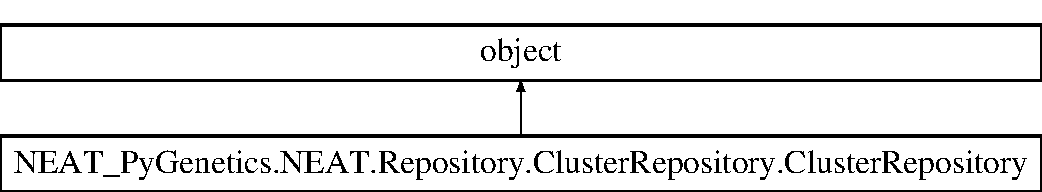
\includegraphics[height=2.000000cm]{classNEAT__PyGenetics_1_1NEAT_1_1Repository_1_1ClusterRepository_1_1ClusterRepository}
\end{center}
\end{figure}
\subsection*{Public Member Functions}
\begin{DoxyCompactItemize}
\item 
def \hyperlink{classNEAT__PyGenetics_1_1NEAT_1_1Repository_1_1ClusterRepository_1_1ClusterRepository_a49b3cd6db6131c52bba0de2481584f20}{\+\_\+\+\_\+init\+\_\+\+\_\+}
\item 
def \hyperlink{classNEAT__PyGenetics_1_1NEAT_1_1Repository_1_1ClusterRepository_1_1ClusterRepository_a06b7a0bc3b6bf0ddc6eb9040dcecd74b}{get\+\_\+current\+\_\+clusters} (self)
\item 
def \hyperlink{classNEAT__PyGenetics_1_1NEAT_1_1Repository_1_1ClusterRepository_1_1ClusterRepository_adab9f634071749a11cfe0875075fb0a5}{add\+\_\+cluster\+\_\+with\+\_\+representative}
\item 
def \hyperlink{classNEAT__PyGenetics_1_1NEAT_1_1Repository_1_1ClusterRepository_1_1ClusterRepository_a58649974b303a672e75c650e69d1cb21}{archive\+\_\+cluster}
\item 
def \hyperlink{classNEAT__PyGenetics_1_1NEAT_1_1Repository_1_1ClusterRepository_1_1ClusterRepository_af79b19639b87ae827067ddb4d23fe83d}{get\+\_\+cluster\+\_\+by\+\_\+representative}
\item 
def \hyperlink{classNEAT__PyGenetics_1_1NEAT_1_1Repository_1_1ClusterRepository_1_1ClusterRepository_aba5e54a8cf88aece8ebb990b812a3ce2}{get\+\_\+cluster\+\_\+count} (self)
\item 
def \hyperlink{classNEAT__PyGenetics_1_1NEAT_1_1Repository_1_1ClusterRepository_1_1ClusterRepository_a40254dd9f12511e8fa3e707b65938db4}{update\+\_\+offspring\+\_\+for\+\_\+cluster}
\item 
def \hyperlink{classNEAT__PyGenetics_1_1NEAT_1_1Repository_1_1ClusterRepository_1_1ClusterRepository_ac0949d637eb75abae63005db57f14700}{update\+\_\+fitness\+\_\+for\+\_\+cluster}
\item 
def \hyperlink{classNEAT__PyGenetics_1_1NEAT_1_1Repository_1_1ClusterRepository_1_1ClusterRepository_a69ed07f142ec57528a44026aba6bd1fe}{update\+\_\+max\+\_\+population\+\_\+for\+\_\+cluster}
\end{DoxyCompactItemize}
\subsection*{Static Public Attributes}
\begin{DoxyCompactItemize}
\item 
\hyperlink{classNEAT__PyGenetics_1_1NEAT_1_1Repository_1_1ClusterRepository_1_1ClusterRepository_a1834515cd9dbbdf31e311ce6a2e8e78a}{cluster}
\item 
\hyperlink{classNEAT__PyGenetics_1_1NEAT_1_1Repository_1_1ClusterRepository_1_1ClusterRepository_accef80a33d0dd0473ad8c9b3723ec0d9}{representative}
\item 
\hyperlink{classNEAT__PyGenetics_1_1NEAT_1_1Repository_1_1ClusterRepository_1_1ClusterRepository_a8d545f61188a41b15f2c7f3fb2fddcec}{offspring}
\end{DoxyCompactItemize}


\subsection{Constructor \& Destructor Documentation}
\index{N\+E\+A\+T\+\_\+\+Py\+Genetics\+::\+N\+E\+A\+T\+::\+Repository\+::\+Cluster\+Repository\+::\+Cluster\+Repository@{N\+E\+A\+T\+\_\+\+Py\+Genetics\+::\+N\+E\+A\+T\+::\+Repository\+::\+Cluster\+Repository\+::\+Cluster\+Repository}!\+\_\+\+\_\+init\+\_\+\+\_\+@{\+\_\+\+\_\+init\+\_\+\+\_\+}}
\index{\+\_\+\+\_\+init\+\_\+\+\_\+@{\+\_\+\+\_\+init\+\_\+\+\_\+}!N\+E\+A\+T\+\_\+\+Py\+Genetics\+::\+N\+E\+A\+T\+::\+Repository\+::\+Cluster\+Repository\+::\+Cluster\+Repository@{N\+E\+A\+T\+\_\+\+Py\+Genetics\+::\+N\+E\+A\+T\+::\+Repository\+::\+Cluster\+Repository\+::\+Cluster\+Repository}}
\subsubsection[{\texorpdfstring{\+\_\+\+\_\+init\+\_\+\+\_\+}{__init__}}]{\setlength{\rightskip}{0pt plus 5cm}def N\+E\+A\+T\+\_\+\+Py\+Genetics.\+N\+E\+A\+T.\+Repository.\+Cluster\+Repository.\+Cluster\+Repository.\+\_\+\+\_\+init\+\_\+\+\_\+ (
\begin{DoxyParamCaption}
\item[{}]{self, }
\item[{}]{database\+\_\+connector}
\end{DoxyParamCaption}
)}\hypertarget{classNEAT__PyGenetics_1_1NEAT_1_1Repository_1_1ClusterRepository_1_1ClusterRepository_a49b3cd6db6131c52bba0de2481584f20}{}\label{classNEAT__PyGenetics_1_1NEAT_1_1Repository_1_1ClusterRepository_1_1ClusterRepository_a49b3cd6db6131c52bba0de2481584f20}


\subsection{Member Function Documentation}
\index{N\+E\+A\+T\+\_\+\+Py\+Genetics\+::\+N\+E\+A\+T\+::\+Repository\+::\+Cluster\+Repository\+::\+Cluster\+Repository@{N\+E\+A\+T\+\_\+\+Py\+Genetics\+::\+N\+E\+A\+T\+::\+Repository\+::\+Cluster\+Repository\+::\+Cluster\+Repository}!add\+\_\+cluster\+\_\+with\+\_\+representative@{add\+\_\+cluster\+\_\+with\+\_\+representative}}
\index{add\+\_\+cluster\+\_\+with\+\_\+representative@{add\+\_\+cluster\+\_\+with\+\_\+representative}!N\+E\+A\+T\+\_\+\+Py\+Genetics\+::\+N\+E\+A\+T\+::\+Repository\+::\+Cluster\+Repository\+::\+Cluster\+Repository@{N\+E\+A\+T\+\_\+\+Py\+Genetics\+::\+N\+E\+A\+T\+::\+Repository\+::\+Cluster\+Repository\+::\+Cluster\+Repository}}
\subsubsection[{\texorpdfstring{add\+\_\+cluster\+\_\+with\+\_\+representative}{add_cluster_with_representative}}]{\setlength{\rightskip}{0pt plus 5cm}def N\+E\+A\+T\+\_\+\+Py\+Genetics.\+N\+E\+A\+T.\+Repository.\+Cluster\+Repository.\+Cluster\+Repository.\+add\+\_\+cluster\+\_\+with\+\_\+representative (
\begin{DoxyParamCaption}
\item[{}]{self, }
\item[{}]{genome\+\_\+id}
\end{DoxyParamCaption}
)}\hypertarget{classNEAT__PyGenetics_1_1NEAT_1_1Repository_1_1ClusterRepository_1_1ClusterRepository_adab9f634071749a11cfe0875075fb0a5}{}\label{classNEAT__PyGenetics_1_1NEAT_1_1Repository_1_1ClusterRepository_1_1ClusterRepository_adab9f634071749a11cfe0875075fb0a5}
\index{N\+E\+A\+T\+\_\+\+Py\+Genetics\+::\+N\+E\+A\+T\+::\+Repository\+::\+Cluster\+Repository\+::\+Cluster\+Repository@{N\+E\+A\+T\+\_\+\+Py\+Genetics\+::\+N\+E\+A\+T\+::\+Repository\+::\+Cluster\+Repository\+::\+Cluster\+Repository}!archive\+\_\+cluster@{archive\+\_\+cluster}}
\index{archive\+\_\+cluster@{archive\+\_\+cluster}!N\+E\+A\+T\+\_\+\+Py\+Genetics\+::\+N\+E\+A\+T\+::\+Repository\+::\+Cluster\+Repository\+::\+Cluster\+Repository@{N\+E\+A\+T\+\_\+\+Py\+Genetics\+::\+N\+E\+A\+T\+::\+Repository\+::\+Cluster\+Repository\+::\+Cluster\+Repository}}
\subsubsection[{\texorpdfstring{archive\+\_\+cluster}{archive_cluster}}]{\setlength{\rightskip}{0pt plus 5cm}def N\+E\+A\+T\+\_\+\+Py\+Genetics.\+N\+E\+A\+T.\+Repository.\+Cluster\+Repository.\+Cluster\+Repository.\+archive\+\_\+cluster (
\begin{DoxyParamCaption}
\item[{}]{self, }
\item[{}]{cluster\+\_\+id}
\end{DoxyParamCaption}
)}\hypertarget{classNEAT__PyGenetics_1_1NEAT_1_1Repository_1_1ClusterRepository_1_1ClusterRepository_a58649974b303a672e75c650e69d1cb21}{}\label{classNEAT__PyGenetics_1_1NEAT_1_1Repository_1_1ClusterRepository_1_1ClusterRepository_a58649974b303a672e75c650e69d1cb21}
\index{N\+E\+A\+T\+\_\+\+Py\+Genetics\+::\+N\+E\+A\+T\+::\+Repository\+::\+Cluster\+Repository\+::\+Cluster\+Repository@{N\+E\+A\+T\+\_\+\+Py\+Genetics\+::\+N\+E\+A\+T\+::\+Repository\+::\+Cluster\+Repository\+::\+Cluster\+Repository}!get\+\_\+cluster\+\_\+by\+\_\+representative@{get\+\_\+cluster\+\_\+by\+\_\+representative}}
\index{get\+\_\+cluster\+\_\+by\+\_\+representative@{get\+\_\+cluster\+\_\+by\+\_\+representative}!N\+E\+A\+T\+\_\+\+Py\+Genetics\+::\+N\+E\+A\+T\+::\+Repository\+::\+Cluster\+Repository\+::\+Cluster\+Repository@{N\+E\+A\+T\+\_\+\+Py\+Genetics\+::\+N\+E\+A\+T\+::\+Repository\+::\+Cluster\+Repository\+::\+Cluster\+Repository}}
\subsubsection[{\texorpdfstring{get\+\_\+cluster\+\_\+by\+\_\+representative}{get_cluster_by_representative}}]{\setlength{\rightskip}{0pt plus 5cm}def N\+E\+A\+T\+\_\+\+Py\+Genetics.\+N\+E\+A\+T.\+Repository.\+Cluster\+Repository.\+Cluster\+Repository.\+get\+\_\+cluster\+\_\+by\+\_\+representative (
\begin{DoxyParamCaption}
\item[{}]{self, }
\item[{}]{genome\+\_\+id}
\end{DoxyParamCaption}
)}\hypertarget{classNEAT__PyGenetics_1_1NEAT_1_1Repository_1_1ClusterRepository_1_1ClusterRepository_af79b19639b87ae827067ddb4d23fe83d}{}\label{classNEAT__PyGenetics_1_1NEAT_1_1Repository_1_1ClusterRepository_1_1ClusterRepository_af79b19639b87ae827067ddb4d23fe83d}
\index{N\+E\+A\+T\+\_\+\+Py\+Genetics\+::\+N\+E\+A\+T\+::\+Repository\+::\+Cluster\+Repository\+::\+Cluster\+Repository@{N\+E\+A\+T\+\_\+\+Py\+Genetics\+::\+N\+E\+A\+T\+::\+Repository\+::\+Cluster\+Repository\+::\+Cluster\+Repository}!get\+\_\+cluster\+\_\+count@{get\+\_\+cluster\+\_\+count}}
\index{get\+\_\+cluster\+\_\+count@{get\+\_\+cluster\+\_\+count}!N\+E\+A\+T\+\_\+\+Py\+Genetics\+::\+N\+E\+A\+T\+::\+Repository\+::\+Cluster\+Repository\+::\+Cluster\+Repository@{N\+E\+A\+T\+\_\+\+Py\+Genetics\+::\+N\+E\+A\+T\+::\+Repository\+::\+Cluster\+Repository\+::\+Cluster\+Repository}}
\subsubsection[{\texorpdfstring{get\+\_\+cluster\+\_\+count(self)}{get_cluster_count(self)}}]{\setlength{\rightskip}{0pt plus 5cm}def N\+E\+A\+T\+\_\+\+Py\+Genetics.\+N\+E\+A\+T.\+Repository.\+Cluster\+Repository.\+Cluster\+Repository.\+get\+\_\+cluster\+\_\+count (
\begin{DoxyParamCaption}
\item[{}]{self, }
\item[{}]{int}
\end{DoxyParamCaption}
)}\hypertarget{classNEAT__PyGenetics_1_1NEAT_1_1Repository_1_1ClusterRepository_1_1ClusterRepository_aba5e54a8cf88aece8ebb990b812a3ce2}{}\label{classNEAT__PyGenetics_1_1NEAT_1_1Repository_1_1ClusterRepository_1_1ClusterRepository_aba5e54a8cf88aece8ebb990b812a3ce2}
\index{N\+E\+A\+T\+\_\+\+Py\+Genetics\+::\+N\+E\+A\+T\+::\+Repository\+::\+Cluster\+Repository\+::\+Cluster\+Repository@{N\+E\+A\+T\+\_\+\+Py\+Genetics\+::\+N\+E\+A\+T\+::\+Repository\+::\+Cluster\+Repository\+::\+Cluster\+Repository}!get\+\_\+current\+\_\+clusters@{get\+\_\+current\+\_\+clusters}}
\index{get\+\_\+current\+\_\+clusters@{get\+\_\+current\+\_\+clusters}!N\+E\+A\+T\+\_\+\+Py\+Genetics\+::\+N\+E\+A\+T\+::\+Repository\+::\+Cluster\+Repository\+::\+Cluster\+Repository@{N\+E\+A\+T\+\_\+\+Py\+Genetics\+::\+N\+E\+A\+T\+::\+Repository\+::\+Cluster\+Repository\+::\+Cluster\+Repository}}
\subsubsection[{\texorpdfstring{get\+\_\+current\+\_\+clusters(self)}{get_current_clusters(self)}}]{\setlength{\rightskip}{0pt plus 5cm}def N\+E\+A\+T\+\_\+\+Py\+Genetics.\+N\+E\+A\+T.\+Repository.\+Cluster\+Repository.\+Cluster\+Repository.\+get\+\_\+current\+\_\+clusters (
\begin{DoxyParamCaption}
\item[{}]{self, }
\item[{}]{List, }
\item[{}]{Cluster}
\end{DoxyParamCaption}
)}\hypertarget{classNEAT__PyGenetics_1_1NEAT_1_1Repository_1_1ClusterRepository_1_1ClusterRepository_a06b7a0bc3b6bf0ddc6eb9040dcecd74b}{}\label{classNEAT__PyGenetics_1_1NEAT_1_1Repository_1_1ClusterRepository_1_1ClusterRepository_a06b7a0bc3b6bf0ddc6eb9040dcecd74b}
\index{N\+E\+A\+T\+\_\+\+Py\+Genetics\+::\+N\+E\+A\+T\+::\+Repository\+::\+Cluster\+Repository\+::\+Cluster\+Repository@{N\+E\+A\+T\+\_\+\+Py\+Genetics\+::\+N\+E\+A\+T\+::\+Repository\+::\+Cluster\+Repository\+::\+Cluster\+Repository}!update\+\_\+fitness\+\_\+for\+\_\+cluster@{update\+\_\+fitness\+\_\+for\+\_\+cluster}}
\index{update\+\_\+fitness\+\_\+for\+\_\+cluster@{update\+\_\+fitness\+\_\+for\+\_\+cluster}!N\+E\+A\+T\+\_\+\+Py\+Genetics\+::\+N\+E\+A\+T\+::\+Repository\+::\+Cluster\+Repository\+::\+Cluster\+Repository@{N\+E\+A\+T\+\_\+\+Py\+Genetics\+::\+N\+E\+A\+T\+::\+Repository\+::\+Cluster\+Repository\+::\+Cluster\+Repository}}
\subsubsection[{\texorpdfstring{update\+\_\+fitness\+\_\+for\+\_\+cluster}{update_fitness_for_cluster}}]{\setlength{\rightskip}{0pt plus 5cm}def N\+E\+A\+T\+\_\+\+Py\+Genetics.\+N\+E\+A\+T.\+Repository.\+Cluster\+Repository.\+Cluster\+Repository.\+update\+\_\+fitness\+\_\+for\+\_\+cluster (
\begin{DoxyParamCaption}
\item[{}]{self, }
\item[{}]{cluster\+\_\+id}
\end{DoxyParamCaption}
)}\hypertarget{classNEAT__PyGenetics_1_1NEAT_1_1Repository_1_1ClusterRepository_1_1ClusterRepository_ac0949d637eb75abae63005db57f14700}{}\label{classNEAT__PyGenetics_1_1NEAT_1_1Repository_1_1ClusterRepository_1_1ClusterRepository_ac0949d637eb75abae63005db57f14700}
\index{N\+E\+A\+T\+\_\+\+Py\+Genetics\+::\+N\+E\+A\+T\+::\+Repository\+::\+Cluster\+Repository\+::\+Cluster\+Repository@{N\+E\+A\+T\+\_\+\+Py\+Genetics\+::\+N\+E\+A\+T\+::\+Repository\+::\+Cluster\+Repository\+::\+Cluster\+Repository}!update\+\_\+max\+\_\+population\+\_\+for\+\_\+cluster@{update\+\_\+max\+\_\+population\+\_\+for\+\_\+cluster}}
\index{update\+\_\+max\+\_\+population\+\_\+for\+\_\+cluster@{update\+\_\+max\+\_\+population\+\_\+for\+\_\+cluster}!N\+E\+A\+T\+\_\+\+Py\+Genetics\+::\+N\+E\+A\+T\+::\+Repository\+::\+Cluster\+Repository\+::\+Cluster\+Repository@{N\+E\+A\+T\+\_\+\+Py\+Genetics\+::\+N\+E\+A\+T\+::\+Repository\+::\+Cluster\+Repository\+::\+Cluster\+Repository}}
\subsubsection[{\texorpdfstring{update\+\_\+max\+\_\+population\+\_\+for\+\_\+cluster}{update_max_population_for_cluster}}]{\setlength{\rightskip}{0pt plus 5cm}def N\+E\+A\+T\+\_\+\+Py\+Genetics.\+N\+E\+A\+T.\+Repository.\+Cluster\+Repository.\+Cluster\+Repository.\+update\+\_\+max\+\_\+population\+\_\+for\+\_\+cluster (
\begin{DoxyParamCaption}
\item[{}]{self, }
\item[{}]{cluster\+\_\+id}
\end{DoxyParamCaption}
)}\hypertarget{classNEAT__PyGenetics_1_1NEAT_1_1Repository_1_1ClusterRepository_1_1ClusterRepository_a69ed07f142ec57528a44026aba6bd1fe}{}\label{classNEAT__PyGenetics_1_1NEAT_1_1Repository_1_1ClusterRepository_1_1ClusterRepository_a69ed07f142ec57528a44026aba6bd1fe}
\index{N\+E\+A\+T\+\_\+\+Py\+Genetics\+::\+N\+E\+A\+T\+::\+Repository\+::\+Cluster\+Repository\+::\+Cluster\+Repository@{N\+E\+A\+T\+\_\+\+Py\+Genetics\+::\+N\+E\+A\+T\+::\+Repository\+::\+Cluster\+Repository\+::\+Cluster\+Repository}!update\+\_\+offspring\+\_\+for\+\_\+cluster@{update\+\_\+offspring\+\_\+for\+\_\+cluster}}
\index{update\+\_\+offspring\+\_\+for\+\_\+cluster@{update\+\_\+offspring\+\_\+for\+\_\+cluster}!N\+E\+A\+T\+\_\+\+Py\+Genetics\+::\+N\+E\+A\+T\+::\+Repository\+::\+Cluster\+Repository\+::\+Cluster\+Repository@{N\+E\+A\+T\+\_\+\+Py\+Genetics\+::\+N\+E\+A\+T\+::\+Repository\+::\+Cluster\+Repository\+::\+Cluster\+Repository}}
\subsubsection[{\texorpdfstring{update\+\_\+offspring\+\_\+for\+\_\+cluster}{update_offspring_for_cluster}}]{\setlength{\rightskip}{0pt plus 5cm}def N\+E\+A\+T\+\_\+\+Py\+Genetics.\+N\+E\+A\+T.\+Repository.\+Cluster\+Repository.\+Cluster\+Repository.\+update\+\_\+offspring\+\_\+for\+\_\+cluster (
\begin{DoxyParamCaption}
\item[{}]{self, }
\item[{}]{cluster\+\_\+id}
\end{DoxyParamCaption}
)}\hypertarget{classNEAT__PyGenetics_1_1NEAT_1_1Repository_1_1ClusterRepository_1_1ClusterRepository_a40254dd9f12511e8fa3e707b65938db4}{}\label{classNEAT__PyGenetics_1_1NEAT_1_1Repository_1_1ClusterRepository_1_1ClusterRepository_a40254dd9f12511e8fa3e707b65938db4}


\subsection{Member Data Documentation}
\index{N\+E\+A\+T\+\_\+\+Py\+Genetics\+::\+N\+E\+A\+T\+::\+Repository\+::\+Cluster\+Repository\+::\+Cluster\+Repository@{N\+E\+A\+T\+\_\+\+Py\+Genetics\+::\+N\+E\+A\+T\+::\+Repository\+::\+Cluster\+Repository\+::\+Cluster\+Repository}!cluster@{cluster}}
\index{cluster@{cluster}!N\+E\+A\+T\+\_\+\+Py\+Genetics\+::\+N\+E\+A\+T\+::\+Repository\+::\+Cluster\+Repository\+::\+Cluster\+Repository@{N\+E\+A\+T\+\_\+\+Py\+Genetics\+::\+N\+E\+A\+T\+::\+Repository\+::\+Cluster\+Repository\+::\+Cluster\+Repository}}
\subsubsection[{\texorpdfstring{cluster}{cluster}}]{\setlength{\rightskip}{0pt plus 5cm}N\+E\+A\+T\+\_\+\+Py\+Genetics.\+N\+E\+A\+T.\+Repository.\+Cluster\+Repository.\+Cluster\+Repository.\+cluster\hspace{0.3cm}{\ttfamily [static]}}\hypertarget{classNEAT__PyGenetics_1_1NEAT_1_1Repository_1_1ClusterRepository_1_1ClusterRepository_a1834515cd9dbbdf31e311ce6a2e8e78a}{}\label{classNEAT__PyGenetics_1_1NEAT_1_1Repository_1_1ClusterRepository_1_1ClusterRepository_a1834515cd9dbbdf31e311ce6a2e8e78a}
\index{N\+E\+A\+T\+\_\+\+Py\+Genetics\+::\+N\+E\+A\+T\+::\+Repository\+::\+Cluster\+Repository\+::\+Cluster\+Repository@{N\+E\+A\+T\+\_\+\+Py\+Genetics\+::\+N\+E\+A\+T\+::\+Repository\+::\+Cluster\+Repository\+::\+Cluster\+Repository}!offspring@{offspring}}
\index{offspring@{offspring}!N\+E\+A\+T\+\_\+\+Py\+Genetics\+::\+N\+E\+A\+T\+::\+Repository\+::\+Cluster\+Repository\+::\+Cluster\+Repository@{N\+E\+A\+T\+\_\+\+Py\+Genetics\+::\+N\+E\+A\+T\+::\+Repository\+::\+Cluster\+Repository\+::\+Cluster\+Repository}}
\subsubsection[{\texorpdfstring{offspring}{offspring}}]{\setlength{\rightskip}{0pt plus 5cm}N\+E\+A\+T\+\_\+\+Py\+Genetics.\+N\+E\+A\+T.\+Repository.\+Cluster\+Repository.\+Cluster\+Repository.\+offspring\hspace{0.3cm}{\ttfamily [static]}}\hypertarget{classNEAT__PyGenetics_1_1NEAT_1_1Repository_1_1ClusterRepository_1_1ClusterRepository_a8d545f61188a41b15f2c7f3fb2fddcec}{}\label{classNEAT__PyGenetics_1_1NEAT_1_1Repository_1_1ClusterRepository_1_1ClusterRepository_a8d545f61188a41b15f2c7f3fb2fddcec}
\index{N\+E\+A\+T\+\_\+\+Py\+Genetics\+::\+N\+E\+A\+T\+::\+Repository\+::\+Cluster\+Repository\+::\+Cluster\+Repository@{N\+E\+A\+T\+\_\+\+Py\+Genetics\+::\+N\+E\+A\+T\+::\+Repository\+::\+Cluster\+Repository\+::\+Cluster\+Repository}!representative@{representative}}
\index{representative@{representative}!N\+E\+A\+T\+\_\+\+Py\+Genetics\+::\+N\+E\+A\+T\+::\+Repository\+::\+Cluster\+Repository\+::\+Cluster\+Repository@{N\+E\+A\+T\+\_\+\+Py\+Genetics\+::\+N\+E\+A\+T\+::\+Repository\+::\+Cluster\+Repository\+::\+Cluster\+Repository}}
\subsubsection[{\texorpdfstring{representative}{representative}}]{\setlength{\rightskip}{0pt plus 5cm}N\+E\+A\+T\+\_\+\+Py\+Genetics.\+N\+E\+A\+T.\+Repository.\+Cluster\+Repository.\+Cluster\+Repository.\+representative\hspace{0.3cm}{\ttfamily [static]}}\hypertarget{classNEAT__PyGenetics_1_1NEAT_1_1Repository_1_1ClusterRepository_1_1ClusterRepository_accef80a33d0dd0473ad8c9b3723ec0d9}{}\label{classNEAT__PyGenetics_1_1NEAT_1_1Repository_1_1ClusterRepository_1_1ClusterRepository_accef80a33d0dd0473ad8c9b3723ec0d9}


The documentation for this class was generated from the following file\+:\begin{DoxyCompactItemize}
\item 
N\+E\+A\+T/\+Repository/\hyperlink{ClusterRepository_8py}{Cluster\+Repository.\+py}\end{DoxyCompactItemize}

\hypertarget{classNEAT__PyGenetics_1_1NEAT_1_1Networking_1_1Commands_1_1CommandTranscoder_1_1CommandTranscoder}{}\section{N\+E\+A\+T\+\_\+\+Py\+Genetics.\+N\+E\+A\+T.\+Networking.\+Commands.\+Command\+Transcoder.\+Command\+Transcoder Class Reference}
\label{classNEAT__PyGenetics_1_1NEAT_1_1Networking_1_1Commands_1_1CommandTranscoder_1_1CommandTranscoder}\index{N\+E\+A\+T\+\_\+\+Py\+Genetics.\+N\+E\+A\+T.\+Networking.\+Commands.\+Command\+Transcoder.\+Command\+Transcoder@{N\+E\+A\+T\+\_\+\+Py\+Genetics.\+N\+E\+A\+T.\+Networking.\+Commands.\+Command\+Transcoder.\+Command\+Transcoder}}
Inheritance diagram for N\+E\+A\+T\+\_\+\+Py\+Genetics.\+N\+E\+A\+T.\+Networking.\+Commands.\+Command\+Transcoder.\+Command\+Transcoder\+:\begin{figure}[H]
\begin{center}
\leavevmode
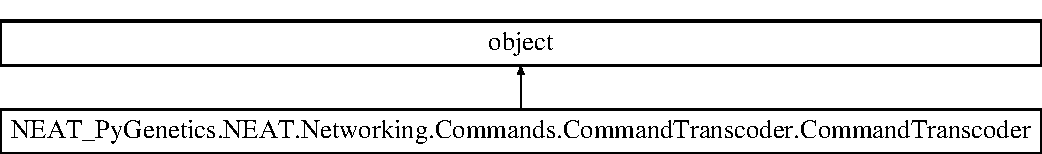
\includegraphics[height=2.000000cm]{classNEAT__PyGenetics_1_1NEAT_1_1Networking_1_1Commands_1_1CommandTranscoder_1_1CommandTranscoder}
\end{center}
\end{figure}
\subsection*{Static Public Member Functions}
\begin{DoxyCompactItemize}
\item 
def \hyperlink{classNEAT__PyGenetics_1_1NEAT_1_1Networking_1_1Commands_1_1CommandTranscoder_1_1CommandTranscoder_a173c5fa30eabf9dc236f761803dfd1df}{encode\+\_\+command}
\item 
def \hyperlink{classNEAT__PyGenetics_1_1NEAT_1_1Networking_1_1Commands_1_1CommandTranscoder_1_1CommandTranscoder_aebdcf1865dd3c040c341f00e88c8d387}{decode\+\_\+command}
\end{DoxyCompactItemize}
\subsection*{Static Public Attributes}
\begin{DoxyCompactItemize}
\item 
\hyperlink{classNEAT__PyGenetics_1_1NEAT_1_1Networking_1_1Commands_1_1CommandTranscoder_1_1CommandTranscoder_a161a64d3c2586008802d174ebc5b6e4b}{type\+\_\+class\+\_\+map}
\end{DoxyCompactItemize}


\subsection{Member Function Documentation}
\index{N\+E\+A\+T\+\_\+\+Py\+Genetics\+::\+N\+E\+A\+T\+::\+Networking\+::\+Commands\+::\+Command\+Transcoder\+::\+Command\+Transcoder@{N\+E\+A\+T\+\_\+\+Py\+Genetics\+::\+N\+E\+A\+T\+::\+Networking\+::\+Commands\+::\+Command\+Transcoder\+::\+Command\+Transcoder}!decode\+\_\+command@{decode\+\_\+command}}
\index{decode\+\_\+command@{decode\+\_\+command}!N\+E\+A\+T\+\_\+\+Py\+Genetics\+::\+N\+E\+A\+T\+::\+Networking\+::\+Commands\+::\+Command\+Transcoder\+::\+Command\+Transcoder@{N\+E\+A\+T\+\_\+\+Py\+Genetics\+::\+N\+E\+A\+T\+::\+Networking\+::\+Commands\+::\+Command\+Transcoder\+::\+Command\+Transcoder}}
\subsubsection[{\texorpdfstring{decode\+\_\+command}{decode_command}}]{\setlength{\rightskip}{0pt plus 5cm}def N\+E\+A\+T\+\_\+\+Py\+Genetics.\+N\+E\+A\+T.\+Networking.\+Commands.\+Command\+Transcoder.\+Command\+Transcoder.\+decode\+\_\+command (
\begin{DoxyParamCaption}
\item[{}]{dictionary}
\end{DoxyParamCaption}
)\hspace{0.3cm}{\ttfamily [static]}}\hypertarget{classNEAT__PyGenetics_1_1NEAT_1_1Networking_1_1Commands_1_1CommandTranscoder_1_1CommandTranscoder_aebdcf1865dd3c040c341f00e88c8d387}{}\label{classNEAT__PyGenetics_1_1NEAT_1_1Networking_1_1Commands_1_1CommandTranscoder_1_1CommandTranscoder_aebdcf1865dd3c040c341f00e88c8d387}
\index{N\+E\+A\+T\+\_\+\+Py\+Genetics\+::\+N\+E\+A\+T\+::\+Networking\+::\+Commands\+::\+Command\+Transcoder\+::\+Command\+Transcoder@{N\+E\+A\+T\+\_\+\+Py\+Genetics\+::\+N\+E\+A\+T\+::\+Networking\+::\+Commands\+::\+Command\+Transcoder\+::\+Command\+Transcoder}!encode\+\_\+command@{encode\+\_\+command}}
\index{encode\+\_\+command@{encode\+\_\+command}!N\+E\+A\+T\+\_\+\+Py\+Genetics\+::\+N\+E\+A\+T\+::\+Networking\+::\+Commands\+::\+Command\+Transcoder\+::\+Command\+Transcoder@{N\+E\+A\+T\+\_\+\+Py\+Genetics\+::\+N\+E\+A\+T\+::\+Networking\+::\+Commands\+::\+Command\+Transcoder\+::\+Command\+Transcoder}}
\subsubsection[{\texorpdfstring{encode\+\_\+command}{encode_command}}]{\setlength{\rightskip}{0pt plus 5cm}def N\+E\+A\+T\+\_\+\+Py\+Genetics.\+N\+E\+A\+T.\+Networking.\+Commands.\+Command\+Transcoder.\+Command\+Transcoder.\+encode\+\_\+command (
\begin{DoxyParamCaption}
\item[{}]{command}
\end{DoxyParamCaption}
)\hspace{0.3cm}{\ttfamily [static]}}\hypertarget{classNEAT__PyGenetics_1_1NEAT_1_1Networking_1_1Commands_1_1CommandTranscoder_1_1CommandTranscoder_a173c5fa30eabf9dc236f761803dfd1df}{}\label{classNEAT__PyGenetics_1_1NEAT_1_1Networking_1_1Commands_1_1CommandTranscoder_1_1CommandTranscoder_a173c5fa30eabf9dc236f761803dfd1df}


\subsection{Member Data Documentation}
\index{N\+E\+A\+T\+\_\+\+Py\+Genetics\+::\+N\+E\+A\+T\+::\+Networking\+::\+Commands\+::\+Command\+Transcoder\+::\+Command\+Transcoder@{N\+E\+A\+T\+\_\+\+Py\+Genetics\+::\+N\+E\+A\+T\+::\+Networking\+::\+Commands\+::\+Command\+Transcoder\+::\+Command\+Transcoder}!type\+\_\+class\+\_\+map@{type\+\_\+class\+\_\+map}}
\index{type\+\_\+class\+\_\+map@{type\+\_\+class\+\_\+map}!N\+E\+A\+T\+\_\+\+Py\+Genetics\+::\+N\+E\+A\+T\+::\+Networking\+::\+Commands\+::\+Command\+Transcoder\+::\+Command\+Transcoder@{N\+E\+A\+T\+\_\+\+Py\+Genetics\+::\+N\+E\+A\+T\+::\+Networking\+::\+Commands\+::\+Command\+Transcoder\+::\+Command\+Transcoder}}
\subsubsection[{\texorpdfstring{type\+\_\+class\+\_\+map}{type_class_map}}]{\setlength{\rightskip}{0pt plus 5cm}N\+E\+A\+T\+\_\+\+Py\+Genetics.\+N\+E\+A\+T.\+Networking.\+Commands.\+Command\+Transcoder.\+Command\+Transcoder.\+type\+\_\+class\+\_\+map\hspace{0.3cm}{\ttfamily [static]}}\hypertarget{classNEAT__PyGenetics_1_1NEAT_1_1Networking_1_1Commands_1_1CommandTranscoder_1_1CommandTranscoder_a161a64d3c2586008802d174ebc5b6e4b}{}\label{classNEAT__PyGenetics_1_1NEAT_1_1Networking_1_1Commands_1_1CommandTranscoder_1_1CommandTranscoder_a161a64d3c2586008802d174ebc5b6e4b}


The documentation for this class was generated from the following file\+:\begin{DoxyCompactItemize}
\item 
N\+E\+A\+T/\+Networking/\+Commands/\hyperlink{CommandTranscoder_8py}{Command\+Transcoder.\+py}\end{DoxyCompactItemize}

\hypertarget{classNEAT__PyGenetics_1_1NEAT_1_1GenomeStructures_1_1SimulationStructure_1_1SimulationNodes_1_1CycleNode}{}\section{N\+E\+A\+T\+\_\+\+Py\+Genetics.\+N\+E\+A\+T.\+Genome\+Structures.\+Simulation\+Structure.\+Simulation\+Nodes.\+Cycle\+Node Class Reference}
\label{classNEAT__PyGenetics_1_1NEAT_1_1GenomeStructures_1_1SimulationStructure_1_1SimulationNodes_1_1CycleNode}\index{N\+E\+A\+T\+\_\+\+Py\+Genetics.\+N\+E\+A\+T.\+Genome\+Structures.\+Simulation\+Structure.\+Simulation\+Nodes.\+Cycle\+Node@{N\+E\+A\+T\+\_\+\+Py\+Genetics.\+N\+E\+A\+T.\+Genome\+Structures.\+Simulation\+Structure.\+Simulation\+Nodes.\+Cycle\+Node}}
Inheritance diagram for N\+E\+A\+T\+\_\+\+Py\+Genetics.\+N\+E\+A\+T.\+Genome\+Structures.\+Simulation\+Structure.\+Simulation\+Nodes.\+Cycle\+Node\+:\begin{figure}[H]
\begin{center}
\leavevmode
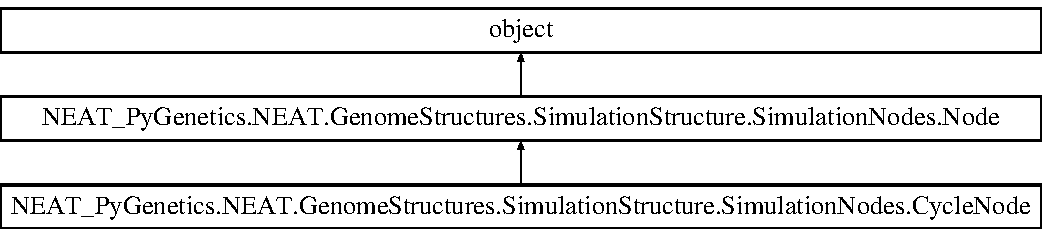
\includegraphics[height=3.000000cm]{classNEAT__PyGenetics_1_1NEAT_1_1GenomeStructures_1_1SimulationStructure_1_1SimulationNodes_1_1CycleNode}
\end{center}
\end{figure}
\subsection*{Public Member Functions}
\begin{DoxyCompactItemize}
\item 
def \hyperlink{classNEAT__PyGenetics_1_1NEAT_1_1GenomeStructures_1_1SimulationStructure_1_1SimulationNodes_1_1CycleNode_a7296250c1afe722523e7897b0ab2b4d4}{\+\_\+\+\_\+init\+\_\+\+\_\+}
\begin{DoxyCompactList}\small\item\em Unlike in \hyperlink{classNEAT__PyGenetics_1_1NEAT_1_1GenomeStructures_1_1SimulationStructure_1_1SimulationNodes_1_1Node}{Node} here the initial\+\_\+value is mandatory. \end{DoxyCompactList}\item 
def \hyperlink{classNEAT__PyGenetics_1_1NEAT_1_1GenomeStructures_1_1SimulationStructure_1_1SimulationNodes_1_1CycleNode_acac910243feebfd38ee9bb9503a4db24}{add\+\_\+cycle\+\_\+successor}
\begin{DoxyCompactList}\small\item\em Adds a cycle successor to the list. \end{DoxyCompactList}\item 
def \hyperlink{classNEAT__PyGenetics_1_1NEAT_1_1GenomeStructures_1_1SimulationStructure_1_1SimulationNodes_1_1CycleNode_a842b0166427a3d54ba9dc87062d2cd57}{add\+\_\+cycle\+\_\+successors}
\begin{DoxyCompactList}\small\item\em Adds multiple successor\+\_\+nodes to the list. \end{DoxyCompactList}\item 
def \hyperlink{classNEAT__PyGenetics_1_1NEAT_1_1GenomeStructures_1_1SimulationStructure_1_1SimulationNodes_1_1CycleNode_aded4c01be2b30e8fc2d0bd89bd4d9763}{fire\+\_\+cycles} (self)
\begin{DoxyCompactList}\small\item\em Adds the last stored value multiplied with the specific weights to all cycle closing successors. \end{DoxyCompactList}\item 
def \hyperlink{classNEAT__PyGenetics_1_1NEAT_1_1GenomeStructures_1_1SimulationStructure_1_1SimulationNodes_1_1CycleNode_a55f0110c03f18c3b093f7cb06354e1e3}{preserve\+\_\+memory} (self)
\begin{DoxyCompactList}\small\item\em Copies the current value into the memory\+\_\+value. \end{DoxyCompactList}\end{DoxyCompactItemize}
\subsection*{Static Public Attributes}
\begin{DoxyCompactItemize}
\item 
\hyperlink{classNEAT__PyGenetics_1_1NEAT_1_1GenomeStructures_1_1SimulationStructure_1_1SimulationNodes_1_1CycleNode_a1af1cde360e80129b245a7db865043e7}{cycle\+\_\+successors}
\item 
\hyperlink{classNEAT__PyGenetics_1_1NEAT_1_1GenomeStructures_1_1SimulationStructure_1_1SimulationNodes_1_1CycleNode_a5d16cbb003056d70af09c3b827ce37bd}{cycle\+\_\+weights}
\item 
\hyperlink{classNEAT__PyGenetics_1_1NEAT_1_1GenomeStructures_1_1SimulationStructure_1_1SimulationNodes_1_1CycleNode_a6bca28573d3931752d70df4440659de3}{memory\+\_\+value}
\end{DoxyCompactItemize}
\subsection*{Additional Inherited Members}


\subsection{Constructor \& Destructor Documentation}
\index{N\+E\+A\+T\+\_\+\+Py\+Genetics\+::\+N\+E\+A\+T\+::\+Genome\+Structures\+::\+Simulation\+Structure\+::\+Simulation\+Nodes\+::\+Cycle\+Node@{N\+E\+A\+T\+\_\+\+Py\+Genetics\+::\+N\+E\+A\+T\+::\+Genome\+Structures\+::\+Simulation\+Structure\+::\+Simulation\+Nodes\+::\+Cycle\+Node}!\+\_\+\+\_\+init\+\_\+\+\_\+@{\+\_\+\+\_\+init\+\_\+\+\_\+}}
\index{\+\_\+\+\_\+init\+\_\+\+\_\+@{\+\_\+\+\_\+init\+\_\+\+\_\+}!N\+E\+A\+T\+\_\+\+Py\+Genetics\+::\+N\+E\+A\+T\+::\+Genome\+Structures\+::\+Simulation\+Structure\+::\+Simulation\+Nodes\+::\+Cycle\+Node@{N\+E\+A\+T\+\_\+\+Py\+Genetics\+::\+N\+E\+A\+T\+::\+Genome\+Structures\+::\+Simulation\+Structure\+::\+Simulation\+Nodes\+::\+Cycle\+Node}}
\subsubsection[{\texorpdfstring{\+\_\+\+\_\+init\+\_\+\+\_\+}{__init__}}]{\setlength{\rightskip}{0pt plus 5cm}def N\+E\+A\+T\+\_\+\+Py\+Genetics.\+N\+E\+A\+T.\+Genome\+Structures.\+Simulation\+Structure.\+Simulation\+Nodes.\+Cycle\+Node.\+\_\+\+\_\+init\+\_\+\+\_\+ (
\begin{DoxyParamCaption}
\item[{}]{self, }
\item[{}]{initial\+\_\+memory\+\_\+value}
\end{DoxyParamCaption}
)}\hypertarget{classNEAT__PyGenetics_1_1NEAT_1_1GenomeStructures_1_1SimulationStructure_1_1SimulationNodes_1_1CycleNode_a7296250c1afe722523e7897b0ab2b4d4}{}\label{classNEAT__PyGenetics_1_1NEAT_1_1GenomeStructures_1_1SimulationStructure_1_1SimulationNodes_1_1CycleNode_a7296250c1afe722523e7897b0ab2b4d4}


Unlike in \hyperlink{classNEAT__PyGenetics_1_1NEAT_1_1GenomeStructures_1_1SimulationStructure_1_1SimulationNodes_1_1Node}{Node} here the initial\+\_\+value is mandatory. 

It is used for the first step of firing the cycle edges. \+:param initial\+\_\+value\+: \+:return\+: 

\subsection{Member Function Documentation}
\index{N\+E\+A\+T\+\_\+\+Py\+Genetics\+::\+N\+E\+A\+T\+::\+Genome\+Structures\+::\+Simulation\+Structure\+::\+Simulation\+Nodes\+::\+Cycle\+Node@{N\+E\+A\+T\+\_\+\+Py\+Genetics\+::\+N\+E\+A\+T\+::\+Genome\+Structures\+::\+Simulation\+Structure\+::\+Simulation\+Nodes\+::\+Cycle\+Node}!add\+\_\+cycle\+\_\+successor@{add\+\_\+cycle\+\_\+successor}}
\index{add\+\_\+cycle\+\_\+successor@{add\+\_\+cycle\+\_\+successor}!N\+E\+A\+T\+\_\+\+Py\+Genetics\+::\+N\+E\+A\+T\+::\+Genome\+Structures\+::\+Simulation\+Structure\+::\+Simulation\+Nodes\+::\+Cycle\+Node@{N\+E\+A\+T\+\_\+\+Py\+Genetics\+::\+N\+E\+A\+T\+::\+Genome\+Structures\+::\+Simulation\+Structure\+::\+Simulation\+Nodes\+::\+Cycle\+Node}}
\subsubsection[{\texorpdfstring{add\+\_\+cycle\+\_\+successor}{add_cycle_successor}}]{\setlength{\rightskip}{0pt plus 5cm}def N\+E\+A\+T\+\_\+\+Py\+Genetics.\+N\+E\+A\+T.\+Genome\+Structures.\+Simulation\+Structure.\+Simulation\+Nodes.\+Cycle\+Node.\+add\+\_\+cycle\+\_\+successor (
\begin{DoxyParamCaption}
\item[{}]{self, }
\item[{}]{successor\+\_\+node}
\end{DoxyParamCaption}
)}\hypertarget{classNEAT__PyGenetics_1_1NEAT_1_1GenomeStructures_1_1SimulationStructure_1_1SimulationNodes_1_1CycleNode_acac910243feebfd38ee9bb9503a4db24}{}\label{classNEAT__PyGenetics_1_1NEAT_1_1GenomeStructures_1_1SimulationStructure_1_1SimulationNodes_1_1CycleNode_acac910243feebfd38ee9bb9503a4db24}


Adds a cycle successor to the list. 

Throws an Exception otherwise. \+:param successor\+\_\+node\+: \+:param weight\+: \+:raises\+: Value\+Error, if the weight of the given nodes is not in the interval \mbox{[}0,1\mbox{]}. \+:raises\+: Exception, if the given successor\+\_\+node already exists in the stored list of successors. \+:return\+: \index{N\+E\+A\+T\+\_\+\+Py\+Genetics\+::\+N\+E\+A\+T\+::\+Genome\+Structures\+::\+Simulation\+Structure\+::\+Simulation\+Nodes\+::\+Cycle\+Node@{N\+E\+A\+T\+\_\+\+Py\+Genetics\+::\+N\+E\+A\+T\+::\+Genome\+Structures\+::\+Simulation\+Structure\+::\+Simulation\+Nodes\+::\+Cycle\+Node}!add\+\_\+cycle\+\_\+successors@{add\+\_\+cycle\+\_\+successors}}
\index{add\+\_\+cycle\+\_\+successors@{add\+\_\+cycle\+\_\+successors}!N\+E\+A\+T\+\_\+\+Py\+Genetics\+::\+N\+E\+A\+T\+::\+Genome\+Structures\+::\+Simulation\+Structure\+::\+Simulation\+Nodes\+::\+Cycle\+Node@{N\+E\+A\+T\+\_\+\+Py\+Genetics\+::\+N\+E\+A\+T\+::\+Genome\+Structures\+::\+Simulation\+Structure\+::\+Simulation\+Nodes\+::\+Cycle\+Node}}
\subsubsection[{\texorpdfstring{add\+\_\+cycle\+\_\+successors}{add_cycle_successors}}]{\setlength{\rightskip}{0pt plus 5cm}def N\+E\+A\+T\+\_\+\+Py\+Genetics.\+N\+E\+A\+T.\+Genome\+Structures.\+Simulation\+Structure.\+Simulation\+Nodes.\+Cycle\+Node.\+add\+\_\+cycle\+\_\+successors (
\begin{DoxyParamCaption}
\item[{}]{self, }
\item[{}]{successor\+\_\+nodes}
\end{DoxyParamCaption}
)}\hypertarget{classNEAT__PyGenetics_1_1NEAT_1_1GenomeStructures_1_1SimulationStructure_1_1SimulationNodes_1_1CycleNode_a842b0166427a3d54ba9dc87062d2cd57}{}\label{classNEAT__PyGenetics_1_1NEAT_1_1GenomeStructures_1_1SimulationStructure_1_1SimulationNodes_1_1CycleNode_a842b0166427a3d54ba9dc87062d2cd57}


Adds multiple successor\+\_\+nodes to the list. 

\+:param successor\+\_\+nodes\+: \+:raises\+: Value\+Error, if the weight of one of the given nodes is not in the interval \mbox{[}0,1\mbox{]}. \+:raises\+: Exception, if one of the given nodes already exists in the stored list of successors. \+:return\+: \index{N\+E\+A\+T\+\_\+\+Py\+Genetics\+::\+N\+E\+A\+T\+::\+Genome\+Structures\+::\+Simulation\+Structure\+::\+Simulation\+Nodes\+::\+Cycle\+Node@{N\+E\+A\+T\+\_\+\+Py\+Genetics\+::\+N\+E\+A\+T\+::\+Genome\+Structures\+::\+Simulation\+Structure\+::\+Simulation\+Nodes\+::\+Cycle\+Node}!fire\+\_\+cycles@{fire\+\_\+cycles}}
\index{fire\+\_\+cycles@{fire\+\_\+cycles}!N\+E\+A\+T\+\_\+\+Py\+Genetics\+::\+N\+E\+A\+T\+::\+Genome\+Structures\+::\+Simulation\+Structure\+::\+Simulation\+Nodes\+::\+Cycle\+Node@{N\+E\+A\+T\+\_\+\+Py\+Genetics\+::\+N\+E\+A\+T\+::\+Genome\+Structures\+::\+Simulation\+Structure\+::\+Simulation\+Nodes\+::\+Cycle\+Node}}
\subsubsection[{\texorpdfstring{fire\+\_\+cycles(self)}{fire_cycles(self)}}]{\setlength{\rightskip}{0pt plus 5cm}def N\+E\+A\+T\+\_\+\+Py\+Genetics.\+N\+E\+A\+T.\+Genome\+Structures.\+Simulation\+Structure.\+Simulation\+Nodes.\+Cycle\+Node.\+fire\+\_\+cycles (
\begin{DoxyParamCaption}
\item[{}]{self, }
\item[{}]{None}
\end{DoxyParamCaption}
)}\hypertarget{classNEAT__PyGenetics_1_1NEAT_1_1GenomeStructures_1_1SimulationStructure_1_1SimulationNodes_1_1CycleNode_aded4c01be2b30e8fc2d0bd89bd4d9763}{}\label{classNEAT__PyGenetics_1_1NEAT_1_1GenomeStructures_1_1SimulationStructure_1_1SimulationNodes_1_1CycleNode_aded4c01be2b30e8fc2d0bd89bd4d9763}


Adds the last stored value multiplied with the specific weights to all cycle closing successors. 

Serves as some kind of short time memory. (Use to be determined) \+:return\+: \index{N\+E\+A\+T\+\_\+\+Py\+Genetics\+::\+N\+E\+A\+T\+::\+Genome\+Structures\+::\+Simulation\+Structure\+::\+Simulation\+Nodes\+::\+Cycle\+Node@{N\+E\+A\+T\+\_\+\+Py\+Genetics\+::\+N\+E\+A\+T\+::\+Genome\+Structures\+::\+Simulation\+Structure\+::\+Simulation\+Nodes\+::\+Cycle\+Node}!preserve\+\_\+memory@{preserve\+\_\+memory}}
\index{preserve\+\_\+memory@{preserve\+\_\+memory}!N\+E\+A\+T\+\_\+\+Py\+Genetics\+::\+N\+E\+A\+T\+::\+Genome\+Structures\+::\+Simulation\+Structure\+::\+Simulation\+Nodes\+::\+Cycle\+Node@{N\+E\+A\+T\+\_\+\+Py\+Genetics\+::\+N\+E\+A\+T\+::\+Genome\+Structures\+::\+Simulation\+Structure\+::\+Simulation\+Nodes\+::\+Cycle\+Node}}
\subsubsection[{\texorpdfstring{preserve\+\_\+memory(self)}{preserve_memory(self)}}]{\setlength{\rightskip}{0pt plus 5cm}def N\+E\+A\+T\+\_\+\+Py\+Genetics.\+N\+E\+A\+T.\+Genome\+Structures.\+Simulation\+Structure.\+Simulation\+Nodes.\+Cycle\+Node.\+preserve\+\_\+memory (
\begin{DoxyParamCaption}
\item[{}]{self, }
\item[{}]{None}
\end{DoxyParamCaption}
)}\hypertarget{classNEAT__PyGenetics_1_1NEAT_1_1GenomeStructures_1_1SimulationStructure_1_1SimulationNodes_1_1CycleNode_a55f0110c03f18c3b093f7cb06354e1e3}{}\label{classNEAT__PyGenetics_1_1NEAT_1_1GenomeStructures_1_1SimulationStructure_1_1SimulationNodes_1_1CycleNode_a55f0110c03f18c3b093f7cb06354e1e3}


Copies the current value into the memory\+\_\+value. 

\+:return\+: 

\subsection{Member Data Documentation}
\index{N\+E\+A\+T\+\_\+\+Py\+Genetics\+::\+N\+E\+A\+T\+::\+Genome\+Structures\+::\+Simulation\+Structure\+::\+Simulation\+Nodes\+::\+Cycle\+Node@{N\+E\+A\+T\+\_\+\+Py\+Genetics\+::\+N\+E\+A\+T\+::\+Genome\+Structures\+::\+Simulation\+Structure\+::\+Simulation\+Nodes\+::\+Cycle\+Node}!cycle\+\_\+successors@{cycle\+\_\+successors}}
\index{cycle\+\_\+successors@{cycle\+\_\+successors}!N\+E\+A\+T\+\_\+\+Py\+Genetics\+::\+N\+E\+A\+T\+::\+Genome\+Structures\+::\+Simulation\+Structure\+::\+Simulation\+Nodes\+::\+Cycle\+Node@{N\+E\+A\+T\+\_\+\+Py\+Genetics\+::\+N\+E\+A\+T\+::\+Genome\+Structures\+::\+Simulation\+Structure\+::\+Simulation\+Nodes\+::\+Cycle\+Node}}
\subsubsection[{\texorpdfstring{cycle\+\_\+successors}{cycle_successors}}]{\setlength{\rightskip}{0pt plus 5cm}N\+E\+A\+T\+\_\+\+Py\+Genetics.\+N\+E\+A\+T.\+Genome\+Structures.\+Simulation\+Structure.\+Simulation\+Nodes.\+Cycle\+Node.\+cycle\+\_\+successors\hspace{0.3cm}{\ttfamily [static]}}\hypertarget{classNEAT__PyGenetics_1_1NEAT_1_1GenomeStructures_1_1SimulationStructure_1_1SimulationNodes_1_1CycleNode_a1af1cde360e80129b245a7db865043e7}{}\label{classNEAT__PyGenetics_1_1NEAT_1_1GenomeStructures_1_1SimulationStructure_1_1SimulationNodes_1_1CycleNode_a1af1cde360e80129b245a7db865043e7}
\index{N\+E\+A\+T\+\_\+\+Py\+Genetics\+::\+N\+E\+A\+T\+::\+Genome\+Structures\+::\+Simulation\+Structure\+::\+Simulation\+Nodes\+::\+Cycle\+Node@{N\+E\+A\+T\+\_\+\+Py\+Genetics\+::\+N\+E\+A\+T\+::\+Genome\+Structures\+::\+Simulation\+Structure\+::\+Simulation\+Nodes\+::\+Cycle\+Node}!cycle\+\_\+weights@{cycle\+\_\+weights}}
\index{cycle\+\_\+weights@{cycle\+\_\+weights}!N\+E\+A\+T\+\_\+\+Py\+Genetics\+::\+N\+E\+A\+T\+::\+Genome\+Structures\+::\+Simulation\+Structure\+::\+Simulation\+Nodes\+::\+Cycle\+Node@{N\+E\+A\+T\+\_\+\+Py\+Genetics\+::\+N\+E\+A\+T\+::\+Genome\+Structures\+::\+Simulation\+Structure\+::\+Simulation\+Nodes\+::\+Cycle\+Node}}
\subsubsection[{\texorpdfstring{cycle\+\_\+weights}{cycle_weights}}]{\setlength{\rightskip}{0pt plus 5cm}N\+E\+A\+T\+\_\+\+Py\+Genetics.\+N\+E\+A\+T.\+Genome\+Structures.\+Simulation\+Structure.\+Simulation\+Nodes.\+Cycle\+Node.\+cycle\+\_\+weights\hspace{0.3cm}{\ttfamily [static]}}\hypertarget{classNEAT__PyGenetics_1_1NEAT_1_1GenomeStructures_1_1SimulationStructure_1_1SimulationNodes_1_1CycleNode_a5d16cbb003056d70af09c3b827ce37bd}{}\label{classNEAT__PyGenetics_1_1NEAT_1_1GenomeStructures_1_1SimulationStructure_1_1SimulationNodes_1_1CycleNode_a5d16cbb003056d70af09c3b827ce37bd}
\index{N\+E\+A\+T\+\_\+\+Py\+Genetics\+::\+N\+E\+A\+T\+::\+Genome\+Structures\+::\+Simulation\+Structure\+::\+Simulation\+Nodes\+::\+Cycle\+Node@{N\+E\+A\+T\+\_\+\+Py\+Genetics\+::\+N\+E\+A\+T\+::\+Genome\+Structures\+::\+Simulation\+Structure\+::\+Simulation\+Nodes\+::\+Cycle\+Node}!memory\+\_\+value@{memory\+\_\+value}}
\index{memory\+\_\+value@{memory\+\_\+value}!N\+E\+A\+T\+\_\+\+Py\+Genetics\+::\+N\+E\+A\+T\+::\+Genome\+Structures\+::\+Simulation\+Structure\+::\+Simulation\+Nodes\+::\+Cycle\+Node@{N\+E\+A\+T\+\_\+\+Py\+Genetics\+::\+N\+E\+A\+T\+::\+Genome\+Structures\+::\+Simulation\+Structure\+::\+Simulation\+Nodes\+::\+Cycle\+Node}}
\subsubsection[{\texorpdfstring{memory\+\_\+value}{memory_value}}]{\setlength{\rightskip}{0pt plus 5cm}N\+E\+A\+T\+\_\+\+Py\+Genetics.\+N\+E\+A\+T.\+Genome\+Structures.\+Simulation\+Structure.\+Simulation\+Nodes.\+Cycle\+Node.\+memory\+\_\+value\hspace{0.3cm}{\ttfamily [static]}}\hypertarget{classNEAT__PyGenetics_1_1NEAT_1_1GenomeStructures_1_1SimulationStructure_1_1SimulationNodes_1_1CycleNode_a6bca28573d3931752d70df4440659de3}{}\label{classNEAT__PyGenetics_1_1NEAT_1_1GenomeStructures_1_1SimulationStructure_1_1SimulationNodes_1_1CycleNode_a6bca28573d3931752d70df4440659de3}


The documentation for this class was generated from the following file\+:\begin{DoxyCompactItemize}
\item 
N\+E\+A\+T/\+Genome\+Structures/\+Simulation\+Structure/\hyperlink{SimulationNodes_8py}{Simulation\+Nodes.\+py}\end{DoxyCompactItemize}

\hypertarget{classNEAT__PyGenetics_1_1NEAT_1_1Repository_1_1DatabaseConnector_1_1DatabaseConnector}{}\section{N\+E\+A\+T\+\_\+\+Py\+Genetics.\+N\+E\+A\+T.\+Repository.\+Database\+Connector.\+Database\+Connector Class Reference}
\label{classNEAT__PyGenetics_1_1NEAT_1_1Repository_1_1DatabaseConnector_1_1DatabaseConnector}\index{N\+E\+A\+T\+\_\+\+Py\+Genetics.\+N\+E\+A\+T.\+Repository.\+Database\+Connector.\+Database\+Connector@{N\+E\+A\+T\+\_\+\+Py\+Genetics.\+N\+E\+A\+T.\+Repository.\+Database\+Connector.\+Database\+Connector}}
Inheritance diagram for N\+E\+A\+T\+\_\+\+Py\+Genetics.\+N\+E\+A\+T.\+Repository.\+Database\+Connector.\+Database\+Connector\+:\begin{figure}[H]
\begin{center}
\leavevmode
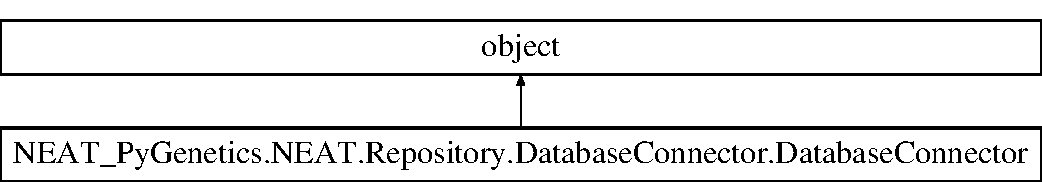
\includegraphics[height=2.000000cm]{classNEAT__PyGenetics_1_1NEAT_1_1Repository_1_1DatabaseConnector_1_1DatabaseConnector}
\end{center}
\end{figure}
\subsection*{Public Member Functions}
\begin{DoxyCompactItemize}
\item 
def \hyperlink{classNEAT__PyGenetics_1_1NEAT_1_1Repository_1_1DatabaseConnector_1_1DatabaseConnector_a57537c32ba05cb1800b4966a9b5ff97f}{\+\_\+\+\_\+init\+\_\+\+\_\+}
\item 
def \hyperlink{classNEAT__PyGenetics_1_1NEAT_1_1Repository_1_1DatabaseConnector_1_1DatabaseConnector_a0531d203c5909eb70a1f328f1ee87e46}{get\+\_\+collection}
\item 
def \hyperlink{classNEAT__PyGenetics_1_1NEAT_1_1Repository_1_1DatabaseConnector_1_1DatabaseConnector_a1c8d38690f25313e30e339bb449e2afc}{insert\+\_\+one}
\begin{DoxyCompactList}\small\item\em Inserts a single object into the given collection in the database. \end{DoxyCompactList}\item 
def \hyperlink{classNEAT__PyGenetics_1_1NEAT_1_1Repository_1_1DatabaseConnector_1_1DatabaseConnector_acaa494840a4f5c9ed45efc87a7b3c9e3}{insert\+\_\+many}
\begin{DoxyCompactList}\small\item\em Inserts multiple objects into the given collection in the database. \end{DoxyCompactList}\item 
def \hyperlink{classNEAT__PyGenetics_1_1NEAT_1_1Repository_1_1DatabaseConnector_1_1DatabaseConnector_a01ed6b2bbdf7e49c3b12260e8f716df0}{find\+\_\+one}
\begin{DoxyCompactList}\small\item\em Finds a single document in the given collection. \end{DoxyCompactList}\item 
def \hyperlink{classNEAT__PyGenetics_1_1NEAT_1_1Repository_1_1DatabaseConnector_1_1DatabaseConnector_ab84e5e82fb7f4ef7e63d1a463f931d0b}{find\+\_\+one\+\_\+by\+\_\+id}
\begin{DoxyCompactList}\small\item\em Finds a single document in the given collection based on its id. \end{DoxyCompactList}\item 
def \hyperlink{classNEAT__PyGenetics_1_1NEAT_1_1Repository_1_1DatabaseConnector_1_1DatabaseConnector_a4f488daecf67131f0a138fbe02d75ad1}{find\+\_\+many}
\begin{DoxyCompactList}\small\item\em Finds all objects in the given collection that match a given query. \end{DoxyCompactList}\item 
def \hyperlink{classNEAT__PyGenetics_1_1NEAT_1_1Repository_1_1DatabaseConnector_1_1DatabaseConnector_a44ca72a0a552c2c68bb6818e3902548e}{update\+\_\+one}
\begin{DoxyCompactList}\small\item\em Updates a single document in the given collection in the database. \end{DoxyCompactList}\item 
def \hyperlink{classNEAT__PyGenetics_1_1NEAT_1_1Repository_1_1DatabaseConnector_1_1DatabaseConnector_a1181a46de443df2c30f65c5585984eab}{update\+\_\+many}
\begin{DoxyCompactList}\small\item\em Updates multiple documents in the given collection in the database. \end{DoxyCompactList}\item 
def \hyperlink{classNEAT__PyGenetics_1_1NEAT_1_1Repository_1_1DatabaseConnector_1_1DatabaseConnector_a562cd964aa44d7e6051d1436acf047ba}{remove\+\_\+one}
\begin{DoxyCompactList}\small\item\em Removes one document by id from a given collection. \end{DoxyCompactList}\item 
def \hyperlink{classNEAT__PyGenetics_1_1NEAT_1_1Repository_1_1DatabaseConnector_1_1DatabaseConnector_ab576f403333ef9dc793d328bd04c41b6}{remove\+\_\+many}
\begin{DoxyCompactList}\small\item\em Removes many documents by id from a given collection. \end{DoxyCompactList}\end{DoxyCompactItemize}
\subsection*{Static Public Attributes}
\begin{DoxyCompactItemize}
\item 
\hyperlink{classNEAT__PyGenetics_1_1NEAT_1_1Repository_1_1DatabaseConnector_1_1DatabaseConnector_ae6a5bd1fe8b17e6f4daeb34016befacc}{result\+\_\+ids}
\item 
\hyperlink{classNEAT__PyGenetics_1_1NEAT_1_1Repository_1_1DatabaseConnector_1_1DatabaseConnector_aa64c3cdec4a68d8b9cb70eff5fc65da1}{i}
\item 
\hyperlink{classNEAT__PyGenetics_1_1NEAT_1_1Repository_1_1DatabaseConnector_1_1DatabaseConnector_ac4e5c7484ac4c90604a438b88250f4cc}{result}
\end{DoxyCompactItemize}


\subsection{Constructor \& Destructor Documentation}
\index{N\+E\+A\+T\+\_\+\+Py\+Genetics\+::\+N\+E\+A\+T\+::\+Repository\+::\+Database\+Connector\+::\+Database\+Connector@{N\+E\+A\+T\+\_\+\+Py\+Genetics\+::\+N\+E\+A\+T\+::\+Repository\+::\+Database\+Connector\+::\+Database\+Connector}!\+\_\+\+\_\+init\+\_\+\+\_\+@{\+\_\+\+\_\+init\+\_\+\+\_\+}}
\index{\+\_\+\+\_\+init\+\_\+\+\_\+@{\+\_\+\+\_\+init\+\_\+\+\_\+}!N\+E\+A\+T\+\_\+\+Py\+Genetics\+::\+N\+E\+A\+T\+::\+Repository\+::\+Database\+Connector\+::\+Database\+Connector@{N\+E\+A\+T\+\_\+\+Py\+Genetics\+::\+N\+E\+A\+T\+::\+Repository\+::\+Database\+Connector\+::\+Database\+Connector}}
\subsubsection[{\texorpdfstring{\+\_\+\+\_\+init\+\_\+\+\_\+}{__init__}}]{\setlength{\rightskip}{0pt plus 5cm}def N\+E\+A\+T\+\_\+\+Py\+Genetics.\+N\+E\+A\+T.\+Repository.\+Database\+Connector.\+Database\+Connector.\+\_\+\+\_\+init\+\_\+\+\_\+ (
\begin{DoxyParamCaption}
\item[{}]{self, }
\item[{}]{database\+\_\+name}
\end{DoxyParamCaption}
)}\hypertarget{classNEAT__PyGenetics_1_1NEAT_1_1Repository_1_1DatabaseConnector_1_1DatabaseConnector_a57537c32ba05cb1800b4966a9b5ff97f}{}\label{classNEAT__PyGenetics_1_1NEAT_1_1Repository_1_1DatabaseConnector_1_1DatabaseConnector_a57537c32ba05cb1800b4966a9b5ff97f}


\subsection{Member Function Documentation}
\index{N\+E\+A\+T\+\_\+\+Py\+Genetics\+::\+N\+E\+A\+T\+::\+Repository\+::\+Database\+Connector\+::\+Database\+Connector@{N\+E\+A\+T\+\_\+\+Py\+Genetics\+::\+N\+E\+A\+T\+::\+Repository\+::\+Database\+Connector\+::\+Database\+Connector}!find\+\_\+many@{find\+\_\+many}}
\index{find\+\_\+many@{find\+\_\+many}!N\+E\+A\+T\+\_\+\+Py\+Genetics\+::\+N\+E\+A\+T\+::\+Repository\+::\+Database\+Connector\+::\+Database\+Connector@{N\+E\+A\+T\+\_\+\+Py\+Genetics\+::\+N\+E\+A\+T\+::\+Repository\+::\+Database\+Connector\+::\+Database\+Connector}}
\subsubsection[{\texorpdfstring{find\+\_\+many}{find_many}}]{\setlength{\rightskip}{0pt plus 5cm}def N\+E\+A\+T\+\_\+\+Py\+Genetics.\+N\+E\+A\+T.\+Repository.\+Database\+Connector.\+Database\+Connector.\+find\+\_\+many (
\begin{DoxyParamCaption}
\item[{}]{self, }
\item[{}]{collection\+\_\+name}
\end{DoxyParamCaption}
)}\hypertarget{classNEAT__PyGenetics_1_1NEAT_1_1Repository_1_1DatabaseConnector_1_1DatabaseConnector_a4f488daecf67131f0a138fbe02d75ad1}{}\label{classNEAT__PyGenetics_1_1NEAT_1_1Repository_1_1DatabaseConnector_1_1DatabaseConnector_a4f488daecf67131f0a138fbe02d75ad1}


Finds all objects in the given collection that match a given query. 

Parameters the same as pymongos default find, except for the collection\+\_\+ name. \+:param collection\+\_\+name\+: \+:param filter\+: \+:return\+: \index{N\+E\+A\+T\+\_\+\+Py\+Genetics\+::\+N\+E\+A\+T\+::\+Repository\+::\+Database\+Connector\+::\+Database\+Connector@{N\+E\+A\+T\+\_\+\+Py\+Genetics\+::\+N\+E\+A\+T\+::\+Repository\+::\+Database\+Connector\+::\+Database\+Connector}!find\+\_\+one@{find\+\_\+one}}
\index{find\+\_\+one@{find\+\_\+one}!N\+E\+A\+T\+\_\+\+Py\+Genetics\+::\+N\+E\+A\+T\+::\+Repository\+::\+Database\+Connector\+::\+Database\+Connector@{N\+E\+A\+T\+\_\+\+Py\+Genetics\+::\+N\+E\+A\+T\+::\+Repository\+::\+Database\+Connector\+::\+Database\+Connector}}
\subsubsection[{\texorpdfstring{find\+\_\+one}{find_one}}]{\setlength{\rightskip}{0pt plus 5cm}def N\+E\+A\+T\+\_\+\+Py\+Genetics.\+N\+E\+A\+T.\+Repository.\+Database\+Connector.\+Database\+Connector.\+find\+\_\+one (
\begin{DoxyParamCaption}
\item[{}]{self, }
\item[{}]{collection\+\_\+name}
\end{DoxyParamCaption}
)}\hypertarget{classNEAT__PyGenetics_1_1NEAT_1_1Repository_1_1DatabaseConnector_1_1DatabaseConnector_a01ed6b2bbdf7e49c3b12260e8f716df0}{}\label{classNEAT__PyGenetics_1_1NEAT_1_1Repository_1_1DatabaseConnector_1_1DatabaseConnector_a01ed6b2bbdf7e49c3b12260e8f716df0}


Finds a single document in the given collection. 

Same parameters as py-\/ mongos default find\+\_\+one, except for the collection\+\_\+name. \+:param collection\+\_\+name\+: \+:param filter\+: \+:return\+: \index{N\+E\+A\+T\+\_\+\+Py\+Genetics\+::\+N\+E\+A\+T\+::\+Repository\+::\+Database\+Connector\+::\+Database\+Connector@{N\+E\+A\+T\+\_\+\+Py\+Genetics\+::\+N\+E\+A\+T\+::\+Repository\+::\+Database\+Connector\+::\+Database\+Connector}!find\+\_\+one\+\_\+by\+\_\+id@{find\+\_\+one\+\_\+by\+\_\+id}}
\index{find\+\_\+one\+\_\+by\+\_\+id@{find\+\_\+one\+\_\+by\+\_\+id}!N\+E\+A\+T\+\_\+\+Py\+Genetics\+::\+N\+E\+A\+T\+::\+Repository\+::\+Database\+Connector\+::\+Database\+Connector@{N\+E\+A\+T\+\_\+\+Py\+Genetics\+::\+N\+E\+A\+T\+::\+Repository\+::\+Database\+Connector\+::\+Database\+Connector}}
\subsubsection[{\texorpdfstring{find\+\_\+one\+\_\+by\+\_\+id}{find_one_by_id}}]{\setlength{\rightskip}{0pt plus 5cm}def N\+E\+A\+T\+\_\+\+Py\+Genetics.\+N\+E\+A\+T.\+Repository.\+Database\+Connector.\+Database\+Connector.\+find\+\_\+one\+\_\+by\+\_\+id (
\begin{DoxyParamCaption}
\item[{}]{self, }
\item[{}]{collection\+\_\+name}
\end{DoxyParamCaption}
)}\hypertarget{classNEAT__PyGenetics_1_1NEAT_1_1Repository_1_1DatabaseConnector_1_1DatabaseConnector_ab84e5e82fb7f4ef7e63d1a463f931d0b}{}\label{classNEAT__PyGenetics_1_1NEAT_1_1Repository_1_1DatabaseConnector_1_1DatabaseConnector_ab84e5e82fb7f4ef7e63d1a463f931d0b}


Finds a single document in the given collection based on its id. 

\+:param collection\+\_\+name\+: \+:param document\+\_\+id\+: \+:return\+: \index{N\+E\+A\+T\+\_\+\+Py\+Genetics\+::\+N\+E\+A\+T\+::\+Repository\+::\+Database\+Connector\+::\+Database\+Connector@{N\+E\+A\+T\+\_\+\+Py\+Genetics\+::\+N\+E\+A\+T\+::\+Repository\+::\+Database\+Connector\+::\+Database\+Connector}!get\+\_\+collection@{get\+\_\+collection}}
\index{get\+\_\+collection@{get\+\_\+collection}!N\+E\+A\+T\+\_\+\+Py\+Genetics\+::\+N\+E\+A\+T\+::\+Repository\+::\+Database\+Connector\+::\+Database\+Connector@{N\+E\+A\+T\+\_\+\+Py\+Genetics\+::\+N\+E\+A\+T\+::\+Repository\+::\+Database\+Connector\+::\+Database\+Connector}}
\subsubsection[{\texorpdfstring{get\+\_\+collection}{get_collection}}]{\setlength{\rightskip}{0pt plus 5cm}def N\+E\+A\+T\+\_\+\+Py\+Genetics.\+N\+E\+A\+T.\+Repository.\+Database\+Connector.\+Database\+Connector.\+get\+\_\+collection (
\begin{DoxyParamCaption}
\item[{}]{self, }
\item[{}]{collection\+\_\+name}
\end{DoxyParamCaption}
)}\hypertarget{classNEAT__PyGenetics_1_1NEAT_1_1Repository_1_1DatabaseConnector_1_1DatabaseConnector_a0531d203c5909eb70a1f328f1ee87e46}{}\label{classNEAT__PyGenetics_1_1NEAT_1_1Repository_1_1DatabaseConnector_1_1DatabaseConnector_a0531d203c5909eb70a1f328f1ee87e46}
\index{N\+E\+A\+T\+\_\+\+Py\+Genetics\+::\+N\+E\+A\+T\+::\+Repository\+::\+Database\+Connector\+::\+Database\+Connector@{N\+E\+A\+T\+\_\+\+Py\+Genetics\+::\+N\+E\+A\+T\+::\+Repository\+::\+Database\+Connector\+::\+Database\+Connector}!insert\+\_\+many@{insert\+\_\+many}}
\index{insert\+\_\+many@{insert\+\_\+many}!N\+E\+A\+T\+\_\+\+Py\+Genetics\+::\+N\+E\+A\+T\+::\+Repository\+::\+Database\+Connector\+::\+Database\+Connector@{N\+E\+A\+T\+\_\+\+Py\+Genetics\+::\+N\+E\+A\+T\+::\+Repository\+::\+Database\+Connector\+::\+Database\+Connector}}
\subsubsection[{\texorpdfstring{insert\+\_\+many}{insert_many}}]{\setlength{\rightskip}{0pt plus 5cm}def N\+E\+A\+T\+\_\+\+Py\+Genetics.\+N\+E\+A\+T.\+Repository.\+Database\+Connector.\+Database\+Connector.\+insert\+\_\+many (
\begin{DoxyParamCaption}
\item[{}]{self, }
\item[{}]{collection\+\_\+name}
\end{DoxyParamCaption}
)}\hypertarget{classNEAT__PyGenetics_1_1NEAT_1_1Repository_1_1DatabaseConnector_1_1DatabaseConnector_acaa494840a4f5c9ed45efc87a7b3c9e3}{}\label{classNEAT__PyGenetics_1_1NEAT_1_1Repository_1_1DatabaseConnector_1_1DatabaseConnector_acaa494840a4f5c9ed45efc87a7b3c9e3}


Inserts multiple objects into the given collection in the database. 

\+:param collection\+\_\+name\+: \+:param documents\+: \+:return\+: \index{N\+E\+A\+T\+\_\+\+Py\+Genetics\+::\+N\+E\+A\+T\+::\+Repository\+::\+Database\+Connector\+::\+Database\+Connector@{N\+E\+A\+T\+\_\+\+Py\+Genetics\+::\+N\+E\+A\+T\+::\+Repository\+::\+Database\+Connector\+::\+Database\+Connector}!insert\+\_\+one@{insert\+\_\+one}}
\index{insert\+\_\+one@{insert\+\_\+one}!N\+E\+A\+T\+\_\+\+Py\+Genetics\+::\+N\+E\+A\+T\+::\+Repository\+::\+Database\+Connector\+::\+Database\+Connector@{N\+E\+A\+T\+\_\+\+Py\+Genetics\+::\+N\+E\+A\+T\+::\+Repository\+::\+Database\+Connector\+::\+Database\+Connector}}
\subsubsection[{\texorpdfstring{insert\+\_\+one}{insert_one}}]{\setlength{\rightskip}{0pt plus 5cm}def N\+E\+A\+T\+\_\+\+Py\+Genetics.\+N\+E\+A\+T.\+Repository.\+Database\+Connector.\+Database\+Connector.\+insert\+\_\+one (
\begin{DoxyParamCaption}
\item[{}]{self, }
\item[{}]{collection\+\_\+name}
\end{DoxyParamCaption}
)}\hypertarget{classNEAT__PyGenetics_1_1NEAT_1_1Repository_1_1DatabaseConnector_1_1DatabaseConnector_a1c8d38690f25313e30e339bb449e2afc}{}\label{classNEAT__PyGenetics_1_1NEAT_1_1Repository_1_1DatabaseConnector_1_1DatabaseConnector_a1c8d38690f25313e30e339bb449e2afc}


Inserts a single object into the given collection in the database. 

\+:param collection\+\_\+name\+: \+:param document\+: \+:return\+: \index{N\+E\+A\+T\+\_\+\+Py\+Genetics\+::\+N\+E\+A\+T\+::\+Repository\+::\+Database\+Connector\+::\+Database\+Connector@{N\+E\+A\+T\+\_\+\+Py\+Genetics\+::\+N\+E\+A\+T\+::\+Repository\+::\+Database\+Connector\+::\+Database\+Connector}!remove\+\_\+many@{remove\+\_\+many}}
\index{remove\+\_\+many@{remove\+\_\+many}!N\+E\+A\+T\+\_\+\+Py\+Genetics\+::\+N\+E\+A\+T\+::\+Repository\+::\+Database\+Connector\+::\+Database\+Connector@{N\+E\+A\+T\+\_\+\+Py\+Genetics\+::\+N\+E\+A\+T\+::\+Repository\+::\+Database\+Connector\+::\+Database\+Connector}}
\subsubsection[{\texorpdfstring{remove\+\_\+many}{remove_many}}]{\setlength{\rightskip}{0pt plus 5cm}def N\+E\+A\+T\+\_\+\+Py\+Genetics.\+N\+E\+A\+T.\+Repository.\+Database\+Connector.\+Database\+Connector.\+remove\+\_\+many (
\begin{DoxyParamCaption}
\item[{}]{self, }
\item[{}]{collection\+\_\+name}
\end{DoxyParamCaption}
)}\hypertarget{classNEAT__PyGenetics_1_1NEAT_1_1Repository_1_1DatabaseConnector_1_1DatabaseConnector_ab576f403333ef9dc793d328bd04c41b6}{}\label{classNEAT__PyGenetics_1_1NEAT_1_1Repository_1_1DatabaseConnector_1_1DatabaseConnector_ab576f403333ef9dc793d328bd04c41b6}


Removes many documents by id from a given collection. 

\+:param collection\+\_\+name\+: \+:param document\+\_\+ids\+: \+:return\+: \index{N\+E\+A\+T\+\_\+\+Py\+Genetics\+::\+N\+E\+A\+T\+::\+Repository\+::\+Database\+Connector\+::\+Database\+Connector@{N\+E\+A\+T\+\_\+\+Py\+Genetics\+::\+N\+E\+A\+T\+::\+Repository\+::\+Database\+Connector\+::\+Database\+Connector}!remove\+\_\+one@{remove\+\_\+one}}
\index{remove\+\_\+one@{remove\+\_\+one}!N\+E\+A\+T\+\_\+\+Py\+Genetics\+::\+N\+E\+A\+T\+::\+Repository\+::\+Database\+Connector\+::\+Database\+Connector@{N\+E\+A\+T\+\_\+\+Py\+Genetics\+::\+N\+E\+A\+T\+::\+Repository\+::\+Database\+Connector\+::\+Database\+Connector}}
\subsubsection[{\texorpdfstring{remove\+\_\+one}{remove_one}}]{\setlength{\rightskip}{0pt plus 5cm}def N\+E\+A\+T\+\_\+\+Py\+Genetics.\+N\+E\+A\+T.\+Repository.\+Database\+Connector.\+Database\+Connector.\+remove\+\_\+one (
\begin{DoxyParamCaption}
\item[{}]{self, }
\item[{}]{collection\+\_\+name}
\end{DoxyParamCaption}
)}\hypertarget{classNEAT__PyGenetics_1_1NEAT_1_1Repository_1_1DatabaseConnector_1_1DatabaseConnector_a562cd964aa44d7e6051d1436acf047ba}{}\label{classNEAT__PyGenetics_1_1NEAT_1_1Repository_1_1DatabaseConnector_1_1DatabaseConnector_a562cd964aa44d7e6051d1436acf047ba}


Removes one document by id from a given collection. 

\+:param collection\+\_\+name\+: \+:param document\+\_\+id\+: \+:return\+: \index{N\+E\+A\+T\+\_\+\+Py\+Genetics\+::\+N\+E\+A\+T\+::\+Repository\+::\+Database\+Connector\+::\+Database\+Connector@{N\+E\+A\+T\+\_\+\+Py\+Genetics\+::\+N\+E\+A\+T\+::\+Repository\+::\+Database\+Connector\+::\+Database\+Connector}!update\+\_\+many@{update\+\_\+many}}
\index{update\+\_\+many@{update\+\_\+many}!N\+E\+A\+T\+\_\+\+Py\+Genetics\+::\+N\+E\+A\+T\+::\+Repository\+::\+Database\+Connector\+::\+Database\+Connector@{N\+E\+A\+T\+\_\+\+Py\+Genetics\+::\+N\+E\+A\+T\+::\+Repository\+::\+Database\+Connector\+::\+Database\+Connector}}
\subsubsection[{\texorpdfstring{update\+\_\+many}{update_many}}]{\setlength{\rightskip}{0pt plus 5cm}def N\+E\+A\+T\+\_\+\+Py\+Genetics.\+N\+E\+A\+T.\+Repository.\+Database\+Connector.\+Database\+Connector.\+update\+\_\+many (
\begin{DoxyParamCaption}
\item[{}]{self, }
\item[{}]{collection\+\_\+name}
\end{DoxyParamCaption}
)}\hypertarget{classNEAT__PyGenetics_1_1NEAT_1_1Repository_1_1DatabaseConnector_1_1DatabaseConnector_a1181a46de443df2c30f65c5585984eab}{}\label{classNEAT__PyGenetics_1_1NEAT_1_1Repository_1_1DatabaseConnector_1_1DatabaseConnector_a1181a46de443df2c30f65c5585984eab}


Updates multiple documents in the given collection in the database. 

Takes an Iterable of document\+\_\+id, object tuples and replaces them one by one in the database. \+:param collection\+\_\+name\+: \+:param documents\+: \+:return\+: information about update process (from mongo\+DB) \index{N\+E\+A\+T\+\_\+\+Py\+Genetics\+::\+N\+E\+A\+T\+::\+Repository\+::\+Database\+Connector\+::\+Database\+Connector@{N\+E\+A\+T\+\_\+\+Py\+Genetics\+::\+N\+E\+A\+T\+::\+Repository\+::\+Database\+Connector\+::\+Database\+Connector}!update\+\_\+one@{update\+\_\+one}}
\index{update\+\_\+one@{update\+\_\+one}!N\+E\+A\+T\+\_\+\+Py\+Genetics\+::\+N\+E\+A\+T\+::\+Repository\+::\+Database\+Connector\+::\+Database\+Connector@{N\+E\+A\+T\+\_\+\+Py\+Genetics\+::\+N\+E\+A\+T\+::\+Repository\+::\+Database\+Connector\+::\+Database\+Connector}}
\subsubsection[{\texorpdfstring{update\+\_\+one}{update_one}}]{\setlength{\rightskip}{0pt plus 5cm}def N\+E\+A\+T\+\_\+\+Py\+Genetics.\+N\+E\+A\+T.\+Repository.\+Database\+Connector.\+Database\+Connector.\+update\+\_\+one (
\begin{DoxyParamCaption}
\item[{}]{self, }
\item[{}]{collection\+\_\+name}
\end{DoxyParamCaption}
)}\hypertarget{classNEAT__PyGenetics_1_1NEAT_1_1Repository_1_1DatabaseConnector_1_1DatabaseConnector_a44ca72a0a552c2c68bb6818e3902548e}{}\label{classNEAT__PyGenetics_1_1NEAT_1_1Repository_1_1DatabaseConnector_1_1DatabaseConnector_a44ca72a0a552c2c68bb6818e3902548e}


Updates a single document in the given collection in the database. 

Takes an id and an object and replaces the data at the given id with the ob-\/ ject. \+:param document\+: \+:param document\+\_\+id\+: \+:param collection\+\_\+name\+: \+:return\+: information about update process (from mongo\+DB) 

\subsection{Member Data Documentation}
\index{N\+E\+A\+T\+\_\+\+Py\+Genetics\+::\+N\+E\+A\+T\+::\+Repository\+::\+Database\+Connector\+::\+Database\+Connector@{N\+E\+A\+T\+\_\+\+Py\+Genetics\+::\+N\+E\+A\+T\+::\+Repository\+::\+Database\+Connector\+::\+Database\+Connector}!i@{i}}
\index{i@{i}!N\+E\+A\+T\+\_\+\+Py\+Genetics\+::\+N\+E\+A\+T\+::\+Repository\+::\+Database\+Connector\+::\+Database\+Connector@{N\+E\+A\+T\+\_\+\+Py\+Genetics\+::\+N\+E\+A\+T\+::\+Repository\+::\+Database\+Connector\+::\+Database\+Connector}}
\subsubsection[{\texorpdfstring{i}{i}}]{\setlength{\rightskip}{0pt plus 5cm}N\+E\+A\+T\+\_\+\+Py\+Genetics.\+N\+E\+A\+T.\+Repository.\+Database\+Connector.\+Database\+Connector.\+i\hspace{0.3cm}{\ttfamily [static]}}\hypertarget{classNEAT__PyGenetics_1_1NEAT_1_1Repository_1_1DatabaseConnector_1_1DatabaseConnector_aa64c3cdec4a68d8b9cb70eff5fc65da1}{}\label{classNEAT__PyGenetics_1_1NEAT_1_1Repository_1_1DatabaseConnector_1_1DatabaseConnector_aa64c3cdec4a68d8b9cb70eff5fc65da1}
\index{N\+E\+A\+T\+\_\+\+Py\+Genetics\+::\+N\+E\+A\+T\+::\+Repository\+::\+Database\+Connector\+::\+Database\+Connector@{N\+E\+A\+T\+\_\+\+Py\+Genetics\+::\+N\+E\+A\+T\+::\+Repository\+::\+Database\+Connector\+::\+Database\+Connector}!result@{result}}
\index{result@{result}!N\+E\+A\+T\+\_\+\+Py\+Genetics\+::\+N\+E\+A\+T\+::\+Repository\+::\+Database\+Connector\+::\+Database\+Connector@{N\+E\+A\+T\+\_\+\+Py\+Genetics\+::\+N\+E\+A\+T\+::\+Repository\+::\+Database\+Connector\+::\+Database\+Connector}}
\subsubsection[{\texorpdfstring{result}{result}}]{\setlength{\rightskip}{0pt plus 5cm}N\+E\+A\+T\+\_\+\+Py\+Genetics.\+N\+E\+A\+T.\+Repository.\+Database\+Connector.\+Database\+Connector.\+result\hspace{0.3cm}{\ttfamily [static]}}\hypertarget{classNEAT__PyGenetics_1_1NEAT_1_1Repository_1_1DatabaseConnector_1_1DatabaseConnector_ac4e5c7484ac4c90604a438b88250f4cc}{}\label{classNEAT__PyGenetics_1_1NEAT_1_1Repository_1_1DatabaseConnector_1_1DatabaseConnector_ac4e5c7484ac4c90604a438b88250f4cc}
\index{N\+E\+A\+T\+\_\+\+Py\+Genetics\+::\+N\+E\+A\+T\+::\+Repository\+::\+Database\+Connector\+::\+Database\+Connector@{N\+E\+A\+T\+\_\+\+Py\+Genetics\+::\+N\+E\+A\+T\+::\+Repository\+::\+Database\+Connector\+::\+Database\+Connector}!result\+\_\+ids@{result\+\_\+ids}}
\index{result\+\_\+ids@{result\+\_\+ids}!N\+E\+A\+T\+\_\+\+Py\+Genetics\+::\+N\+E\+A\+T\+::\+Repository\+::\+Database\+Connector\+::\+Database\+Connector@{N\+E\+A\+T\+\_\+\+Py\+Genetics\+::\+N\+E\+A\+T\+::\+Repository\+::\+Database\+Connector\+::\+Database\+Connector}}
\subsubsection[{\texorpdfstring{result\+\_\+ids}{result_ids}}]{\setlength{\rightskip}{0pt plus 5cm}N\+E\+A\+T\+\_\+\+Py\+Genetics.\+N\+E\+A\+T.\+Repository.\+Database\+Connector.\+Database\+Connector.\+result\+\_\+ids\hspace{0.3cm}{\ttfamily [static]}}\hypertarget{classNEAT__PyGenetics_1_1NEAT_1_1Repository_1_1DatabaseConnector_1_1DatabaseConnector_ae6a5bd1fe8b17e6f4daeb34016befacc}{}\label{classNEAT__PyGenetics_1_1NEAT_1_1Repository_1_1DatabaseConnector_1_1DatabaseConnector_ae6a5bd1fe8b17e6f4daeb34016befacc}


The documentation for this class was generated from the following file\+:\begin{DoxyCompactItemize}
\item 
N\+E\+A\+T/\+Repository/\hyperlink{DatabaseConnector_8py}{Database\+Connector.\+py}\end{DoxyCompactItemize}

\hypertarget{classNEAT__PyGenetics_1_1NEAT_1_1Tests_1_1RepositoryTests_1_1test__databaseConnector_1_1DatabaseConnectorTest}{}\section{N\+E\+A\+T\+\_\+\+Py\+Genetics.\+N\+E\+A\+T.\+Tests.\+Repository\+Tests.\+test\+\_\+database\+Connector.\+Database\+Connector\+Test Class Reference}
\label{classNEAT__PyGenetics_1_1NEAT_1_1Tests_1_1RepositoryTests_1_1test__databaseConnector_1_1DatabaseConnectorTest}\index{N\+E\+A\+T\+\_\+\+Py\+Genetics.\+N\+E\+A\+T.\+Tests.\+Repository\+Tests.\+test\+\_\+database\+Connector.\+Database\+Connector\+Test@{N\+E\+A\+T\+\_\+\+Py\+Genetics.\+N\+E\+A\+T.\+Tests.\+Repository\+Tests.\+test\+\_\+database\+Connector.\+Database\+Connector\+Test}}
Inheritance diagram for N\+E\+A\+T\+\_\+\+Py\+Genetics.\+N\+E\+A\+T.\+Tests.\+Repository\+Tests.\+test\+\_\+database\+Connector.\+Database\+Connector\+Test\+:\begin{figure}[H]
\begin{center}
\leavevmode
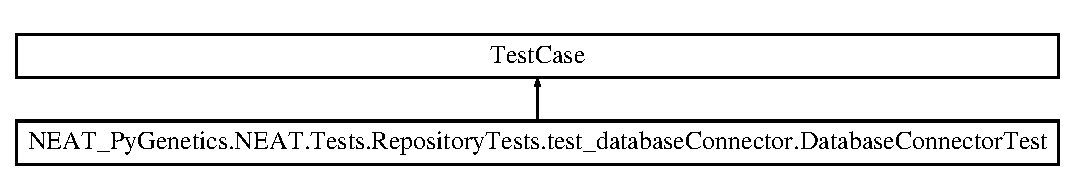
\includegraphics[height=1.978799cm]{classNEAT__PyGenetics_1_1NEAT_1_1Tests_1_1RepositoryTests_1_1test__databaseConnector_1_1DatabaseConnectorTest}
\end{center}
\end{figure}
\subsection*{Public Member Functions}
\begin{DoxyCompactItemize}
\item 
def \hyperlink{classNEAT__PyGenetics_1_1NEAT_1_1Tests_1_1RepositoryTests_1_1test__databaseConnector_1_1DatabaseConnectorTest_a91d61974260986974a20508255b4ac15}{set\+Up} (self)
\item 
def \hyperlink{classNEAT__PyGenetics_1_1NEAT_1_1Tests_1_1RepositoryTests_1_1test__databaseConnector_1_1DatabaseConnectorTest_af5c978077be86b490cb1fc5ddd45b8a6}{test\+\_\+get\+Collection} (self)
\item 
def \hyperlink{classNEAT__PyGenetics_1_1NEAT_1_1Tests_1_1RepositoryTests_1_1test__databaseConnector_1_1DatabaseConnectorTest_a0cb8fdc59961c49884fc3eedbc7f3dd5}{test\+\_\+insert\+One} (self)
\item 
def \hyperlink{classNEAT__PyGenetics_1_1NEAT_1_1Tests_1_1RepositoryTests_1_1test__databaseConnector_1_1DatabaseConnectorTest_a98a79c5760b6dc3f2157af53fe6001a3}{test\+\_\+insert\+Many} (self)
\item 
def \hyperlink{classNEAT__PyGenetics_1_1NEAT_1_1Tests_1_1RepositoryTests_1_1test__databaseConnector_1_1DatabaseConnectorTest_a7ea0327574316e92b1b866b823639e09}{test\+\_\+find\+One} (self)
\item 
def \hyperlink{classNEAT__PyGenetics_1_1NEAT_1_1Tests_1_1RepositoryTests_1_1test__databaseConnector_1_1DatabaseConnectorTest_a903ee479fb3ef1432cdf9fd4e1464e5e}{test\+\_\+find\+One\+By\+Id} (self)
\item 
def \hyperlink{classNEAT__PyGenetics_1_1NEAT_1_1Tests_1_1RepositoryTests_1_1test__databaseConnector_1_1DatabaseConnectorTest_a08ec69775b40a8081e3e09b85ff35969}{test\+\_\+find\+Many} (self)
\item 
def \hyperlink{classNEAT__PyGenetics_1_1NEAT_1_1Tests_1_1RepositoryTests_1_1test__databaseConnector_1_1DatabaseConnectorTest_a2b589e245c56dad59a11844c5c273c2f}{test\+\_\+update\+One} (self)
\item 
def \hyperlink{classNEAT__PyGenetics_1_1NEAT_1_1Tests_1_1RepositoryTests_1_1test__databaseConnector_1_1DatabaseConnectorTest_a9b491c21b224c52ae6f7309fb49eedf5}{test\+\_\+update\+Many\+Fail} (self)
\item 
def \hyperlink{classNEAT__PyGenetics_1_1NEAT_1_1Tests_1_1RepositoryTests_1_1test__databaseConnector_1_1DatabaseConnectorTest_a515f4b176113719b0198bfa91647c63e}{test\+\_\+update\+Many} (self)
\item 
def \hyperlink{classNEAT__PyGenetics_1_1NEAT_1_1Tests_1_1RepositoryTests_1_1test__databaseConnector_1_1DatabaseConnectorTest_a14bc136f4338528fb46c51925d89c7ac}{test\+\_\+remove\+One} (self)
\item 
def \hyperlink{classNEAT__PyGenetics_1_1NEAT_1_1Tests_1_1RepositoryTests_1_1test__databaseConnector_1_1DatabaseConnectorTest_a86194fa471e1217076ee3a080790b82d}{test\+\_\+remove\+Many} (self)
\end{DoxyCompactItemize}
\subsection*{Public Attributes}
\begin{DoxyCompactItemize}
\item 
\hyperlink{classNEAT__PyGenetics_1_1NEAT_1_1Tests_1_1RepositoryTests_1_1test__databaseConnector_1_1DatabaseConnectorTest_a9115740100acd95dbd3a72371acfe681}{db}
\item 
\hyperlink{classNEAT__PyGenetics_1_1NEAT_1_1Tests_1_1RepositoryTests_1_1test__databaseConnector_1_1DatabaseConnectorTest_aca0cb75295bf0c9964cceef08fa98b7b}{collection}
\item 
\hyperlink{classNEAT__PyGenetics_1_1NEAT_1_1Tests_1_1RepositoryTests_1_1test__databaseConnector_1_1DatabaseConnectorTest_aafa6c5991087684c1187c529c8f76682}{database\+\_\+connector}
\end{DoxyCompactItemize}


\subsection{Member Function Documentation}
\index{N\+E\+A\+T\+\_\+\+Py\+Genetics\+::\+N\+E\+A\+T\+::\+Tests\+::\+Repository\+Tests\+::test\+\_\+database\+Connector\+::\+Database\+Connector\+Test@{N\+E\+A\+T\+\_\+\+Py\+Genetics\+::\+N\+E\+A\+T\+::\+Tests\+::\+Repository\+Tests\+::test\+\_\+database\+Connector\+::\+Database\+Connector\+Test}!set\+Up@{set\+Up}}
\index{set\+Up@{set\+Up}!N\+E\+A\+T\+\_\+\+Py\+Genetics\+::\+N\+E\+A\+T\+::\+Tests\+::\+Repository\+Tests\+::test\+\_\+database\+Connector\+::\+Database\+Connector\+Test@{N\+E\+A\+T\+\_\+\+Py\+Genetics\+::\+N\+E\+A\+T\+::\+Tests\+::\+Repository\+Tests\+::test\+\_\+database\+Connector\+::\+Database\+Connector\+Test}}
\subsubsection[{\texorpdfstring{set\+Up(self)}{setUp(self)}}]{\setlength{\rightskip}{0pt plus 5cm}def N\+E\+A\+T\+\_\+\+Py\+Genetics.\+N\+E\+A\+T.\+Tests.\+Repository\+Tests.\+test\+\_\+database\+Connector.\+Database\+Connector\+Test.\+set\+Up (
\begin{DoxyParamCaption}
\item[{}]{self}
\end{DoxyParamCaption}
)}\hypertarget{classNEAT__PyGenetics_1_1NEAT_1_1Tests_1_1RepositoryTests_1_1test__databaseConnector_1_1DatabaseConnectorTest_a91d61974260986974a20508255b4ac15}{}\label{classNEAT__PyGenetics_1_1NEAT_1_1Tests_1_1RepositoryTests_1_1test__databaseConnector_1_1DatabaseConnectorTest_a91d61974260986974a20508255b4ac15}
\index{N\+E\+A\+T\+\_\+\+Py\+Genetics\+::\+N\+E\+A\+T\+::\+Tests\+::\+Repository\+Tests\+::test\+\_\+database\+Connector\+::\+Database\+Connector\+Test@{N\+E\+A\+T\+\_\+\+Py\+Genetics\+::\+N\+E\+A\+T\+::\+Tests\+::\+Repository\+Tests\+::test\+\_\+database\+Connector\+::\+Database\+Connector\+Test}!test\+\_\+find\+Many@{test\+\_\+find\+Many}}
\index{test\+\_\+find\+Many@{test\+\_\+find\+Many}!N\+E\+A\+T\+\_\+\+Py\+Genetics\+::\+N\+E\+A\+T\+::\+Tests\+::\+Repository\+Tests\+::test\+\_\+database\+Connector\+::\+Database\+Connector\+Test@{N\+E\+A\+T\+\_\+\+Py\+Genetics\+::\+N\+E\+A\+T\+::\+Tests\+::\+Repository\+Tests\+::test\+\_\+database\+Connector\+::\+Database\+Connector\+Test}}
\subsubsection[{\texorpdfstring{test\+\_\+find\+Many(self)}{test_findMany(self)}}]{\setlength{\rightskip}{0pt plus 5cm}def N\+E\+A\+T\+\_\+\+Py\+Genetics.\+N\+E\+A\+T.\+Tests.\+Repository\+Tests.\+test\+\_\+database\+Connector.\+Database\+Connector\+Test.\+test\+\_\+find\+Many (
\begin{DoxyParamCaption}
\item[{}]{self}
\end{DoxyParamCaption}
)}\hypertarget{classNEAT__PyGenetics_1_1NEAT_1_1Tests_1_1RepositoryTests_1_1test__databaseConnector_1_1DatabaseConnectorTest_a08ec69775b40a8081e3e09b85ff35969}{}\label{classNEAT__PyGenetics_1_1NEAT_1_1Tests_1_1RepositoryTests_1_1test__databaseConnector_1_1DatabaseConnectorTest_a08ec69775b40a8081e3e09b85ff35969}
\index{N\+E\+A\+T\+\_\+\+Py\+Genetics\+::\+N\+E\+A\+T\+::\+Tests\+::\+Repository\+Tests\+::test\+\_\+database\+Connector\+::\+Database\+Connector\+Test@{N\+E\+A\+T\+\_\+\+Py\+Genetics\+::\+N\+E\+A\+T\+::\+Tests\+::\+Repository\+Tests\+::test\+\_\+database\+Connector\+::\+Database\+Connector\+Test}!test\+\_\+find\+One@{test\+\_\+find\+One}}
\index{test\+\_\+find\+One@{test\+\_\+find\+One}!N\+E\+A\+T\+\_\+\+Py\+Genetics\+::\+N\+E\+A\+T\+::\+Tests\+::\+Repository\+Tests\+::test\+\_\+database\+Connector\+::\+Database\+Connector\+Test@{N\+E\+A\+T\+\_\+\+Py\+Genetics\+::\+N\+E\+A\+T\+::\+Tests\+::\+Repository\+Tests\+::test\+\_\+database\+Connector\+::\+Database\+Connector\+Test}}
\subsubsection[{\texorpdfstring{test\+\_\+find\+One(self)}{test_findOne(self)}}]{\setlength{\rightskip}{0pt plus 5cm}def N\+E\+A\+T\+\_\+\+Py\+Genetics.\+N\+E\+A\+T.\+Tests.\+Repository\+Tests.\+test\+\_\+database\+Connector.\+Database\+Connector\+Test.\+test\+\_\+find\+One (
\begin{DoxyParamCaption}
\item[{}]{self}
\end{DoxyParamCaption}
)}\hypertarget{classNEAT__PyGenetics_1_1NEAT_1_1Tests_1_1RepositoryTests_1_1test__databaseConnector_1_1DatabaseConnectorTest_a7ea0327574316e92b1b866b823639e09}{}\label{classNEAT__PyGenetics_1_1NEAT_1_1Tests_1_1RepositoryTests_1_1test__databaseConnector_1_1DatabaseConnectorTest_a7ea0327574316e92b1b866b823639e09}
\index{N\+E\+A\+T\+\_\+\+Py\+Genetics\+::\+N\+E\+A\+T\+::\+Tests\+::\+Repository\+Tests\+::test\+\_\+database\+Connector\+::\+Database\+Connector\+Test@{N\+E\+A\+T\+\_\+\+Py\+Genetics\+::\+N\+E\+A\+T\+::\+Tests\+::\+Repository\+Tests\+::test\+\_\+database\+Connector\+::\+Database\+Connector\+Test}!test\+\_\+find\+One\+By\+Id@{test\+\_\+find\+One\+By\+Id}}
\index{test\+\_\+find\+One\+By\+Id@{test\+\_\+find\+One\+By\+Id}!N\+E\+A\+T\+\_\+\+Py\+Genetics\+::\+N\+E\+A\+T\+::\+Tests\+::\+Repository\+Tests\+::test\+\_\+database\+Connector\+::\+Database\+Connector\+Test@{N\+E\+A\+T\+\_\+\+Py\+Genetics\+::\+N\+E\+A\+T\+::\+Tests\+::\+Repository\+Tests\+::test\+\_\+database\+Connector\+::\+Database\+Connector\+Test}}
\subsubsection[{\texorpdfstring{test\+\_\+find\+One\+By\+Id(self)}{test_findOneById(self)}}]{\setlength{\rightskip}{0pt plus 5cm}def N\+E\+A\+T\+\_\+\+Py\+Genetics.\+N\+E\+A\+T.\+Tests.\+Repository\+Tests.\+test\+\_\+database\+Connector.\+Database\+Connector\+Test.\+test\+\_\+find\+One\+By\+Id (
\begin{DoxyParamCaption}
\item[{}]{self}
\end{DoxyParamCaption}
)}\hypertarget{classNEAT__PyGenetics_1_1NEAT_1_1Tests_1_1RepositoryTests_1_1test__databaseConnector_1_1DatabaseConnectorTest_a903ee479fb3ef1432cdf9fd4e1464e5e}{}\label{classNEAT__PyGenetics_1_1NEAT_1_1Tests_1_1RepositoryTests_1_1test__databaseConnector_1_1DatabaseConnectorTest_a903ee479fb3ef1432cdf9fd4e1464e5e}
\index{N\+E\+A\+T\+\_\+\+Py\+Genetics\+::\+N\+E\+A\+T\+::\+Tests\+::\+Repository\+Tests\+::test\+\_\+database\+Connector\+::\+Database\+Connector\+Test@{N\+E\+A\+T\+\_\+\+Py\+Genetics\+::\+N\+E\+A\+T\+::\+Tests\+::\+Repository\+Tests\+::test\+\_\+database\+Connector\+::\+Database\+Connector\+Test}!test\+\_\+get\+Collection@{test\+\_\+get\+Collection}}
\index{test\+\_\+get\+Collection@{test\+\_\+get\+Collection}!N\+E\+A\+T\+\_\+\+Py\+Genetics\+::\+N\+E\+A\+T\+::\+Tests\+::\+Repository\+Tests\+::test\+\_\+database\+Connector\+::\+Database\+Connector\+Test@{N\+E\+A\+T\+\_\+\+Py\+Genetics\+::\+N\+E\+A\+T\+::\+Tests\+::\+Repository\+Tests\+::test\+\_\+database\+Connector\+::\+Database\+Connector\+Test}}
\subsubsection[{\texorpdfstring{test\+\_\+get\+Collection(self)}{test_getCollection(self)}}]{\setlength{\rightskip}{0pt plus 5cm}def N\+E\+A\+T\+\_\+\+Py\+Genetics.\+N\+E\+A\+T.\+Tests.\+Repository\+Tests.\+test\+\_\+database\+Connector.\+Database\+Connector\+Test.\+test\+\_\+get\+Collection (
\begin{DoxyParamCaption}
\item[{}]{self}
\end{DoxyParamCaption}
)}\hypertarget{classNEAT__PyGenetics_1_1NEAT_1_1Tests_1_1RepositoryTests_1_1test__databaseConnector_1_1DatabaseConnectorTest_af5c978077be86b490cb1fc5ddd45b8a6}{}\label{classNEAT__PyGenetics_1_1NEAT_1_1Tests_1_1RepositoryTests_1_1test__databaseConnector_1_1DatabaseConnectorTest_af5c978077be86b490cb1fc5ddd45b8a6}
\index{N\+E\+A\+T\+\_\+\+Py\+Genetics\+::\+N\+E\+A\+T\+::\+Tests\+::\+Repository\+Tests\+::test\+\_\+database\+Connector\+::\+Database\+Connector\+Test@{N\+E\+A\+T\+\_\+\+Py\+Genetics\+::\+N\+E\+A\+T\+::\+Tests\+::\+Repository\+Tests\+::test\+\_\+database\+Connector\+::\+Database\+Connector\+Test}!test\+\_\+insert\+Many@{test\+\_\+insert\+Many}}
\index{test\+\_\+insert\+Many@{test\+\_\+insert\+Many}!N\+E\+A\+T\+\_\+\+Py\+Genetics\+::\+N\+E\+A\+T\+::\+Tests\+::\+Repository\+Tests\+::test\+\_\+database\+Connector\+::\+Database\+Connector\+Test@{N\+E\+A\+T\+\_\+\+Py\+Genetics\+::\+N\+E\+A\+T\+::\+Tests\+::\+Repository\+Tests\+::test\+\_\+database\+Connector\+::\+Database\+Connector\+Test}}
\subsubsection[{\texorpdfstring{test\+\_\+insert\+Many(self)}{test_insertMany(self)}}]{\setlength{\rightskip}{0pt plus 5cm}def N\+E\+A\+T\+\_\+\+Py\+Genetics.\+N\+E\+A\+T.\+Tests.\+Repository\+Tests.\+test\+\_\+database\+Connector.\+Database\+Connector\+Test.\+test\+\_\+insert\+Many (
\begin{DoxyParamCaption}
\item[{}]{self}
\end{DoxyParamCaption}
)}\hypertarget{classNEAT__PyGenetics_1_1NEAT_1_1Tests_1_1RepositoryTests_1_1test__databaseConnector_1_1DatabaseConnectorTest_a98a79c5760b6dc3f2157af53fe6001a3}{}\label{classNEAT__PyGenetics_1_1NEAT_1_1Tests_1_1RepositoryTests_1_1test__databaseConnector_1_1DatabaseConnectorTest_a98a79c5760b6dc3f2157af53fe6001a3}
\index{N\+E\+A\+T\+\_\+\+Py\+Genetics\+::\+N\+E\+A\+T\+::\+Tests\+::\+Repository\+Tests\+::test\+\_\+database\+Connector\+::\+Database\+Connector\+Test@{N\+E\+A\+T\+\_\+\+Py\+Genetics\+::\+N\+E\+A\+T\+::\+Tests\+::\+Repository\+Tests\+::test\+\_\+database\+Connector\+::\+Database\+Connector\+Test}!test\+\_\+insert\+One@{test\+\_\+insert\+One}}
\index{test\+\_\+insert\+One@{test\+\_\+insert\+One}!N\+E\+A\+T\+\_\+\+Py\+Genetics\+::\+N\+E\+A\+T\+::\+Tests\+::\+Repository\+Tests\+::test\+\_\+database\+Connector\+::\+Database\+Connector\+Test@{N\+E\+A\+T\+\_\+\+Py\+Genetics\+::\+N\+E\+A\+T\+::\+Tests\+::\+Repository\+Tests\+::test\+\_\+database\+Connector\+::\+Database\+Connector\+Test}}
\subsubsection[{\texorpdfstring{test\+\_\+insert\+One(self)}{test_insertOne(self)}}]{\setlength{\rightskip}{0pt plus 5cm}def N\+E\+A\+T\+\_\+\+Py\+Genetics.\+N\+E\+A\+T.\+Tests.\+Repository\+Tests.\+test\+\_\+database\+Connector.\+Database\+Connector\+Test.\+test\+\_\+insert\+One (
\begin{DoxyParamCaption}
\item[{}]{self}
\end{DoxyParamCaption}
)}\hypertarget{classNEAT__PyGenetics_1_1NEAT_1_1Tests_1_1RepositoryTests_1_1test__databaseConnector_1_1DatabaseConnectorTest_a0cb8fdc59961c49884fc3eedbc7f3dd5}{}\label{classNEAT__PyGenetics_1_1NEAT_1_1Tests_1_1RepositoryTests_1_1test__databaseConnector_1_1DatabaseConnectorTest_a0cb8fdc59961c49884fc3eedbc7f3dd5}
\index{N\+E\+A\+T\+\_\+\+Py\+Genetics\+::\+N\+E\+A\+T\+::\+Tests\+::\+Repository\+Tests\+::test\+\_\+database\+Connector\+::\+Database\+Connector\+Test@{N\+E\+A\+T\+\_\+\+Py\+Genetics\+::\+N\+E\+A\+T\+::\+Tests\+::\+Repository\+Tests\+::test\+\_\+database\+Connector\+::\+Database\+Connector\+Test}!test\+\_\+remove\+Many@{test\+\_\+remove\+Many}}
\index{test\+\_\+remove\+Many@{test\+\_\+remove\+Many}!N\+E\+A\+T\+\_\+\+Py\+Genetics\+::\+N\+E\+A\+T\+::\+Tests\+::\+Repository\+Tests\+::test\+\_\+database\+Connector\+::\+Database\+Connector\+Test@{N\+E\+A\+T\+\_\+\+Py\+Genetics\+::\+N\+E\+A\+T\+::\+Tests\+::\+Repository\+Tests\+::test\+\_\+database\+Connector\+::\+Database\+Connector\+Test}}
\subsubsection[{\texorpdfstring{test\+\_\+remove\+Many(self)}{test_removeMany(self)}}]{\setlength{\rightskip}{0pt plus 5cm}def N\+E\+A\+T\+\_\+\+Py\+Genetics.\+N\+E\+A\+T.\+Tests.\+Repository\+Tests.\+test\+\_\+database\+Connector.\+Database\+Connector\+Test.\+test\+\_\+remove\+Many (
\begin{DoxyParamCaption}
\item[{}]{self}
\end{DoxyParamCaption}
)}\hypertarget{classNEAT__PyGenetics_1_1NEAT_1_1Tests_1_1RepositoryTests_1_1test__databaseConnector_1_1DatabaseConnectorTest_a86194fa471e1217076ee3a080790b82d}{}\label{classNEAT__PyGenetics_1_1NEAT_1_1Tests_1_1RepositoryTests_1_1test__databaseConnector_1_1DatabaseConnectorTest_a86194fa471e1217076ee3a080790b82d}
\index{N\+E\+A\+T\+\_\+\+Py\+Genetics\+::\+N\+E\+A\+T\+::\+Tests\+::\+Repository\+Tests\+::test\+\_\+database\+Connector\+::\+Database\+Connector\+Test@{N\+E\+A\+T\+\_\+\+Py\+Genetics\+::\+N\+E\+A\+T\+::\+Tests\+::\+Repository\+Tests\+::test\+\_\+database\+Connector\+::\+Database\+Connector\+Test}!test\+\_\+remove\+One@{test\+\_\+remove\+One}}
\index{test\+\_\+remove\+One@{test\+\_\+remove\+One}!N\+E\+A\+T\+\_\+\+Py\+Genetics\+::\+N\+E\+A\+T\+::\+Tests\+::\+Repository\+Tests\+::test\+\_\+database\+Connector\+::\+Database\+Connector\+Test@{N\+E\+A\+T\+\_\+\+Py\+Genetics\+::\+N\+E\+A\+T\+::\+Tests\+::\+Repository\+Tests\+::test\+\_\+database\+Connector\+::\+Database\+Connector\+Test}}
\subsubsection[{\texorpdfstring{test\+\_\+remove\+One(self)}{test_removeOne(self)}}]{\setlength{\rightskip}{0pt plus 5cm}def N\+E\+A\+T\+\_\+\+Py\+Genetics.\+N\+E\+A\+T.\+Tests.\+Repository\+Tests.\+test\+\_\+database\+Connector.\+Database\+Connector\+Test.\+test\+\_\+remove\+One (
\begin{DoxyParamCaption}
\item[{}]{self}
\end{DoxyParamCaption}
)}\hypertarget{classNEAT__PyGenetics_1_1NEAT_1_1Tests_1_1RepositoryTests_1_1test__databaseConnector_1_1DatabaseConnectorTest_a14bc136f4338528fb46c51925d89c7ac}{}\label{classNEAT__PyGenetics_1_1NEAT_1_1Tests_1_1RepositoryTests_1_1test__databaseConnector_1_1DatabaseConnectorTest_a14bc136f4338528fb46c51925d89c7ac}
\index{N\+E\+A\+T\+\_\+\+Py\+Genetics\+::\+N\+E\+A\+T\+::\+Tests\+::\+Repository\+Tests\+::test\+\_\+database\+Connector\+::\+Database\+Connector\+Test@{N\+E\+A\+T\+\_\+\+Py\+Genetics\+::\+N\+E\+A\+T\+::\+Tests\+::\+Repository\+Tests\+::test\+\_\+database\+Connector\+::\+Database\+Connector\+Test}!test\+\_\+update\+Many@{test\+\_\+update\+Many}}
\index{test\+\_\+update\+Many@{test\+\_\+update\+Many}!N\+E\+A\+T\+\_\+\+Py\+Genetics\+::\+N\+E\+A\+T\+::\+Tests\+::\+Repository\+Tests\+::test\+\_\+database\+Connector\+::\+Database\+Connector\+Test@{N\+E\+A\+T\+\_\+\+Py\+Genetics\+::\+N\+E\+A\+T\+::\+Tests\+::\+Repository\+Tests\+::test\+\_\+database\+Connector\+::\+Database\+Connector\+Test}}
\subsubsection[{\texorpdfstring{test\+\_\+update\+Many(self)}{test_updateMany(self)}}]{\setlength{\rightskip}{0pt plus 5cm}def N\+E\+A\+T\+\_\+\+Py\+Genetics.\+N\+E\+A\+T.\+Tests.\+Repository\+Tests.\+test\+\_\+database\+Connector.\+Database\+Connector\+Test.\+test\+\_\+update\+Many (
\begin{DoxyParamCaption}
\item[{}]{self}
\end{DoxyParamCaption}
)}\hypertarget{classNEAT__PyGenetics_1_1NEAT_1_1Tests_1_1RepositoryTests_1_1test__databaseConnector_1_1DatabaseConnectorTest_a515f4b176113719b0198bfa91647c63e}{}\label{classNEAT__PyGenetics_1_1NEAT_1_1Tests_1_1RepositoryTests_1_1test__databaseConnector_1_1DatabaseConnectorTest_a515f4b176113719b0198bfa91647c63e}
\index{N\+E\+A\+T\+\_\+\+Py\+Genetics\+::\+N\+E\+A\+T\+::\+Tests\+::\+Repository\+Tests\+::test\+\_\+database\+Connector\+::\+Database\+Connector\+Test@{N\+E\+A\+T\+\_\+\+Py\+Genetics\+::\+N\+E\+A\+T\+::\+Tests\+::\+Repository\+Tests\+::test\+\_\+database\+Connector\+::\+Database\+Connector\+Test}!test\+\_\+update\+Many\+Fail@{test\+\_\+update\+Many\+Fail}}
\index{test\+\_\+update\+Many\+Fail@{test\+\_\+update\+Many\+Fail}!N\+E\+A\+T\+\_\+\+Py\+Genetics\+::\+N\+E\+A\+T\+::\+Tests\+::\+Repository\+Tests\+::test\+\_\+database\+Connector\+::\+Database\+Connector\+Test@{N\+E\+A\+T\+\_\+\+Py\+Genetics\+::\+N\+E\+A\+T\+::\+Tests\+::\+Repository\+Tests\+::test\+\_\+database\+Connector\+::\+Database\+Connector\+Test}}
\subsubsection[{\texorpdfstring{test\+\_\+update\+Many\+Fail(self)}{test_updateManyFail(self)}}]{\setlength{\rightskip}{0pt plus 5cm}def N\+E\+A\+T\+\_\+\+Py\+Genetics.\+N\+E\+A\+T.\+Tests.\+Repository\+Tests.\+test\+\_\+database\+Connector.\+Database\+Connector\+Test.\+test\+\_\+update\+Many\+Fail (
\begin{DoxyParamCaption}
\item[{}]{self}
\end{DoxyParamCaption}
)}\hypertarget{classNEAT__PyGenetics_1_1NEAT_1_1Tests_1_1RepositoryTests_1_1test__databaseConnector_1_1DatabaseConnectorTest_a9b491c21b224c52ae6f7309fb49eedf5}{}\label{classNEAT__PyGenetics_1_1NEAT_1_1Tests_1_1RepositoryTests_1_1test__databaseConnector_1_1DatabaseConnectorTest_a9b491c21b224c52ae6f7309fb49eedf5}
\index{N\+E\+A\+T\+\_\+\+Py\+Genetics\+::\+N\+E\+A\+T\+::\+Tests\+::\+Repository\+Tests\+::test\+\_\+database\+Connector\+::\+Database\+Connector\+Test@{N\+E\+A\+T\+\_\+\+Py\+Genetics\+::\+N\+E\+A\+T\+::\+Tests\+::\+Repository\+Tests\+::test\+\_\+database\+Connector\+::\+Database\+Connector\+Test}!test\+\_\+update\+One@{test\+\_\+update\+One}}
\index{test\+\_\+update\+One@{test\+\_\+update\+One}!N\+E\+A\+T\+\_\+\+Py\+Genetics\+::\+N\+E\+A\+T\+::\+Tests\+::\+Repository\+Tests\+::test\+\_\+database\+Connector\+::\+Database\+Connector\+Test@{N\+E\+A\+T\+\_\+\+Py\+Genetics\+::\+N\+E\+A\+T\+::\+Tests\+::\+Repository\+Tests\+::test\+\_\+database\+Connector\+::\+Database\+Connector\+Test}}
\subsubsection[{\texorpdfstring{test\+\_\+update\+One(self)}{test_updateOne(self)}}]{\setlength{\rightskip}{0pt plus 5cm}def N\+E\+A\+T\+\_\+\+Py\+Genetics.\+N\+E\+A\+T.\+Tests.\+Repository\+Tests.\+test\+\_\+database\+Connector.\+Database\+Connector\+Test.\+test\+\_\+update\+One (
\begin{DoxyParamCaption}
\item[{}]{self}
\end{DoxyParamCaption}
)}\hypertarget{classNEAT__PyGenetics_1_1NEAT_1_1Tests_1_1RepositoryTests_1_1test__databaseConnector_1_1DatabaseConnectorTest_a2b589e245c56dad59a11844c5c273c2f}{}\label{classNEAT__PyGenetics_1_1NEAT_1_1Tests_1_1RepositoryTests_1_1test__databaseConnector_1_1DatabaseConnectorTest_a2b589e245c56dad59a11844c5c273c2f}


\subsection{Member Data Documentation}
\index{N\+E\+A\+T\+\_\+\+Py\+Genetics\+::\+N\+E\+A\+T\+::\+Tests\+::\+Repository\+Tests\+::test\+\_\+database\+Connector\+::\+Database\+Connector\+Test@{N\+E\+A\+T\+\_\+\+Py\+Genetics\+::\+N\+E\+A\+T\+::\+Tests\+::\+Repository\+Tests\+::test\+\_\+database\+Connector\+::\+Database\+Connector\+Test}!collection@{collection}}
\index{collection@{collection}!N\+E\+A\+T\+\_\+\+Py\+Genetics\+::\+N\+E\+A\+T\+::\+Tests\+::\+Repository\+Tests\+::test\+\_\+database\+Connector\+::\+Database\+Connector\+Test@{N\+E\+A\+T\+\_\+\+Py\+Genetics\+::\+N\+E\+A\+T\+::\+Tests\+::\+Repository\+Tests\+::test\+\_\+database\+Connector\+::\+Database\+Connector\+Test}}
\subsubsection[{\texorpdfstring{collection}{collection}}]{\setlength{\rightskip}{0pt plus 5cm}N\+E\+A\+T\+\_\+\+Py\+Genetics.\+N\+E\+A\+T.\+Tests.\+Repository\+Tests.\+test\+\_\+database\+Connector.\+Database\+Connector\+Test.\+collection}\hypertarget{classNEAT__PyGenetics_1_1NEAT_1_1Tests_1_1RepositoryTests_1_1test__databaseConnector_1_1DatabaseConnectorTest_aca0cb75295bf0c9964cceef08fa98b7b}{}\label{classNEAT__PyGenetics_1_1NEAT_1_1Tests_1_1RepositoryTests_1_1test__databaseConnector_1_1DatabaseConnectorTest_aca0cb75295bf0c9964cceef08fa98b7b}
\index{N\+E\+A\+T\+\_\+\+Py\+Genetics\+::\+N\+E\+A\+T\+::\+Tests\+::\+Repository\+Tests\+::test\+\_\+database\+Connector\+::\+Database\+Connector\+Test@{N\+E\+A\+T\+\_\+\+Py\+Genetics\+::\+N\+E\+A\+T\+::\+Tests\+::\+Repository\+Tests\+::test\+\_\+database\+Connector\+::\+Database\+Connector\+Test}!database\+\_\+connector@{database\+\_\+connector}}
\index{database\+\_\+connector@{database\+\_\+connector}!N\+E\+A\+T\+\_\+\+Py\+Genetics\+::\+N\+E\+A\+T\+::\+Tests\+::\+Repository\+Tests\+::test\+\_\+database\+Connector\+::\+Database\+Connector\+Test@{N\+E\+A\+T\+\_\+\+Py\+Genetics\+::\+N\+E\+A\+T\+::\+Tests\+::\+Repository\+Tests\+::test\+\_\+database\+Connector\+::\+Database\+Connector\+Test}}
\subsubsection[{\texorpdfstring{database\+\_\+connector}{database_connector}}]{\setlength{\rightskip}{0pt plus 5cm}N\+E\+A\+T\+\_\+\+Py\+Genetics.\+N\+E\+A\+T.\+Tests.\+Repository\+Tests.\+test\+\_\+database\+Connector.\+Database\+Connector\+Test.\+database\+\_\+connector}\hypertarget{classNEAT__PyGenetics_1_1NEAT_1_1Tests_1_1RepositoryTests_1_1test__databaseConnector_1_1DatabaseConnectorTest_aafa6c5991087684c1187c529c8f76682}{}\label{classNEAT__PyGenetics_1_1NEAT_1_1Tests_1_1RepositoryTests_1_1test__databaseConnector_1_1DatabaseConnectorTest_aafa6c5991087684c1187c529c8f76682}
\index{N\+E\+A\+T\+\_\+\+Py\+Genetics\+::\+N\+E\+A\+T\+::\+Tests\+::\+Repository\+Tests\+::test\+\_\+database\+Connector\+::\+Database\+Connector\+Test@{N\+E\+A\+T\+\_\+\+Py\+Genetics\+::\+N\+E\+A\+T\+::\+Tests\+::\+Repository\+Tests\+::test\+\_\+database\+Connector\+::\+Database\+Connector\+Test}!db@{db}}
\index{db@{db}!N\+E\+A\+T\+\_\+\+Py\+Genetics\+::\+N\+E\+A\+T\+::\+Tests\+::\+Repository\+Tests\+::test\+\_\+database\+Connector\+::\+Database\+Connector\+Test@{N\+E\+A\+T\+\_\+\+Py\+Genetics\+::\+N\+E\+A\+T\+::\+Tests\+::\+Repository\+Tests\+::test\+\_\+database\+Connector\+::\+Database\+Connector\+Test}}
\subsubsection[{\texorpdfstring{db}{db}}]{\setlength{\rightskip}{0pt plus 5cm}N\+E\+A\+T\+\_\+\+Py\+Genetics.\+N\+E\+A\+T.\+Tests.\+Repository\+Tests.\+test\+\_\+database\+Connector.\+Database\+Connector\+Test.\+db}\hypertarget{classNEAT__PyGenetics_1_1NEAT_1_1Tests_1_1RepositoryTests_1_1test__databaseConnector_1_1DatabaseConnectorTest_a9115740100acd95dbd3a72371acfe681}{}\label{classNEAT__PyGenetics_1_1NEAT_1_1Tests_1_1RepositoryTests_1_1test__databaseConnector_1_1DatabaseConnectorTest_a9115740100acd95dbd3a72371acfe681}


The documentation for this class was generated from the following file\+:\begin{DoxyCompactItemize}
\item 
N\+E\+A\+T/\+Tests/\+Repository\+Tests/\hyperlink{test__databaseConnector_8py}{test\+\_\+database\+Connector.\+py}\end{DoxyCompactItemize}

\hypertarget{classNEAT__PyGenetics_1_1NEAT_1_1Decisions_1_1DecisionMaker_1_1DecisionMaker}{}\section{N\+E\+A\+T\+\_\+\+Py\+Genetics.\+N\+E\+A\+T.\+Decisions.\+Decision\+Maker.\+Decision\+Maker Class Reference}
\label{classNEAT__PyGenetics_1_1NEAT_1_1Decisions_1_1DecisionMaker_1_1DecisionMaker}\index{N\+E\+A\+T\+\_\+\+Py\+Genetics.\+N\+E\+A\+T.\+Decisions.\+Decision\+Maker.\+Decision\+Maker@{N\+E\+A\+T\+\_\+\+Py\+Genetics.\+N\+E\+A\+T.\+Decisions.\+Decision\+Maker.\+Decision\+Maker}}
Inheritance diagram for N\+E\+A\+T\+\_\+\+Py\+Genetics.\+N\+E\+A\+T.\+Decisions.\+Decision\+Maker.\+Decision\+Maker\+:\begin{figure}[H]
\begin{center}
\leavevmode
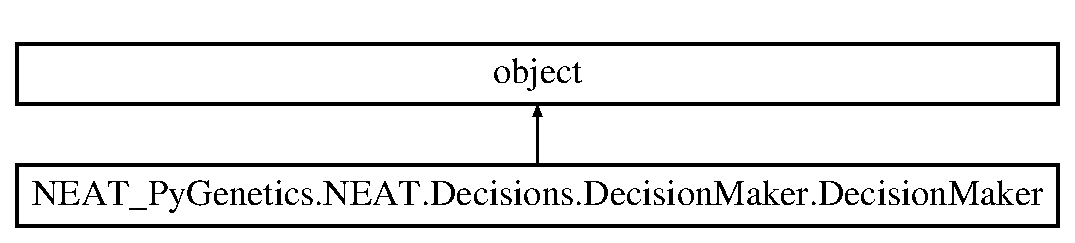
\includegraphics[height=2.000000cm]{classNEAT__PyGenetics_1_1NEAT_1_1Decisions_1_1DecisionMaker_1_1DecisionMaker}
\end{center}
\end{figure}
\subsection*{Public Member Functions}
\begin{DoxyCompactItemize}
\item 
def \hyperlink{classNEAT__PyGenetics_1_1NEAT_1_1Decisions_1_1DecisionMaker_1_1DecisionMaker_a7691e28dc58fcd50858edcbf206c5bd9}{\+\_\+\+\_\+init\+\_\+\+\_\+} (self, decision\+\_\+making\+\_\+parameters)
\item 
def \hyperlink{classNEAT__PyGenetics_1_1NEAT_1_1Decisions_1_1DecisionMaker_1_1DecisionMaker_aee1f2396d8dfe5fd8e47f86bf6ffdb84}{advance\+\_\+time} (self)
\item 
def \hyperlink{classNEAT__PyGenetics_1_1NEAT_1_1Decisions_1_1DecisionMaker_1_1DecisionMaker_a18ac18ed4d2954404ea8b58e45b2f176}{reset\+\_\+time} (self)
\item 
def \hyperlink{classNEAT__PyGenetics_1_1NEAT_1_1Decisions_1_1DecisionMaker_1_1DecisionMaker_ac441f750aa9b1853744bf49b5e195249}{mutation\+\_\+percentage} (self)
\item 
def \hyperlink{classNEAT__PyGenetics_1_1NEAT_1_1Decisions_1_1DecisionMaker_1_1DecisionMaker_ab7cf16b4c29f75b24dec3c6f887b1cea}{inter\+\_\+cluster\+\_\+breeding\+\_\+time} (self)
\end{DoxyCompactItemize}


\subsection{Constructor \& Destructor Documentation}
\index{N\+E\+A\+T\+\_\+\+Py\+Genetics\+::\+N\+E\+A\+T\+::\+Decisions\+::\+Decision\+Maker\+::\+Decision\+Maker@{N\+E\+A\+T\+\_\+\+Py\+Genetics\+::\+N\+E\+A\+T\+::\+Decisions\+::\+Decision\+Maker\+::\+Decision\+Maker}!\+\_\+\+\_\+init\+\_\+\+\_\+@{\+\_\+\+\_\+init\+\_\+\+\_\+}}
\index{\+\_\+\+\_\+init\+\_\+\+\_\+@{\+\_\+\+\_\+init\+\_\+\+\_\+}!N\+E\+A\+T\+\_\+\+Py\+Genetics\+::\+N\+E\+A\+T\+::\+Decisions\+::\+Decision\+Maker\+::\+Decision\+Maker@{N\+E\+A\+T\+\_\+\+Py\+Genetics\+::\+N\+E\+A\+T\+::\+Decisions\+::\+Decision\+Maker\+::\+Decision\+Maker}}
\subsubsection[{\texorpdfstring{\+\_\+\+\_\+init\+\_\+\+\_\+(self, decision\+\_\+making\+\_\+parameters)}{__init__(self, decision_making_parameters)}}]{\setlength{\rightskip}{0pt plus 5cm}def N\+E\+A\+T\+\_\+\+Py\+Genetics.\+N\+E\+A\+T.\+Decisions.\+Decision\+Maker.\+Decision\+Maker.\+\_\+\+\_\+init\+\_\+\+\_\+ (
\begin{DoxyParamCaption}
\item[{}]{self, }
\item[{}]{decision\+\_\+making\+\_\+parameters}
\end{DoxyParamCaption}
)}\hypertarget{classNEAT__PyGenetics_1_1NEAT_1_1Decisions_1_1DecisionMaker_1_1DecisionMaker_a7691e28dc58fcd50858edcbf206c5bd9}{}\label{classNEAT__PyGenetics_1_1NEAT_1_1Decisions_1_1DecisionMaker_1_1DecisionMaker_a7691e28dc58fcd50858edcbf206c5bd9}


\subsection{Member Function Documentation}
\index{N\+E\+A\+T\+\_\+\+Py\+Genetics\+::\+N\+E\+A\+T\+::\+Decisions\+::\+Decision\+Maker\+::\+Decision\+Maker@{N\+E\+A\+T\+\_\+\+Py\+Genetics\+::\+N\+E\+A\+T\+::\+Decisions\+::\+Decision\+Maker\+::\+Decision\+Maker}!advance\+\_\+time@{advance\+\_\+time}}
\index{advance\+\_\+time@{advance\+\_\+time}!N\+E\+A\+T\+\_\+\+Py\+Genetics\+::\+N\+E\+A\+T\+::\+Decisions\+::\+Decision\+Maker\+::\+Decision\+Maker@{N\+E\+A\+T\+\_\+\+Py\+Genetics\+::\+N\+E\+A\+T\+::\+Decisions\+::\+Decision\+Maker\+::\+Decision\+Maker}}
\subsubsection[{\texorpdfstring{advance\+\_\+time(self)}{advance_time(self)}}]{\setlength{\rightskip}{0pt plus 5cm}def N\+E\+A\+T\+\_\+\+Py\+Genetics.\+N\+E\+A\+T.\+Decisions.\+Decision\+Maker.\+Decision\+Maker.\+advance\+\_\+time (
\begin{DoxyParamCaption}
\item[{}]{self}
\end{DoxyParamCaption}
)}\hypertarget{classNEAT__PyGenetics_1_1NEAT_1_1Decisions_1_1DecisionMaker_1_1DecisionMaker_aee1f2396d8dfe5fd8e47f86bf6ffdb84}{}\label{classNEAT__PyGenetics_1_1NEAT_1_1Decisions_1_1DecisionMaker_1_1DecisionMaker_aee1f2396d8dfe5fd8e47f86bf6ffdb84}
\index{N\+E\+A\+T\+\_\+\+Py\+Genetics\+::\+N\+E\+A\+T\+::\+Decisions\+::\+Decision\+Maker\+::\+Decision\+Maker@{N\+E\+A\+T\+\_\+\+Py\+Genetics\+::\+N\+E\+A\+T\+::\+Decisions\+::\+Decision\+Maker\+::\+Decision\+Maker}!inter\+\_\+cluster\+\_\+breeding\+\_\+time@{inter\+\_\+cluster\+\_\+breeding\+\_\+time}}
\index{inter\+\_\+cluster\+\_\+breeding\+\_\+time@{inter\+\_\+cluster\+\_\+breeding\+\_\+time}!N\+E\+A\+T\+\_\+\+Py\+Genetics\+::\+N\+E\+A\+T\+::\+Decisions\+::\+Decision\+Maker\+::\+Decision\+Maker@{N\+E\+A\+T\+\_\+\+Py\+Genetics\+::\+N\+E\+A\+T\+::\+Decisions\+::\+Decision\+Maker\+::\+Decision\+Maker}}
\subsubsection[{\texorpdfstring{inter\+\_\+cluster\+\_\+breeding\+\_\+time(self)}{inter_cluster_breeding_time(self)}}]{\setlength{\rightskip}{0pt plus 5cm}def N\+E\+A\+T\+\_\+\+Py\+Genetics.\+N\+E\+A\+T.\+Decisions.\+Decision\+Maker.\+Decision\+Maker.\+inter\+\_\+cluster\+\_\+breeding\+\_\+time (
\begin{DoxyParamCaption}
\item[{}]{self}
\end{DoxyParamCaption}
)}\hypertarget{classNEAT__PyGenetics_1_1NEAT_1_1Decisions_1_1DecisionMaker_1_1DecisionMaker_ab7cf16b4c29f75b24dec3c6f887b1cea}{}\label{classNEAT__PyGenetics_1_1NEAT_1_1Decisions_1_1DecisionMaker_1_1DecisionMaker_ab7cf16b4c29f75b24dec3c6f887b1cea}
\index{N\+E\+A\+T\+\_\+\+Py\+Genetics\+::\+N\+E\+A\+T\+::\+Decisions\+::\+Decision\+Maker\+::\+Decision\+Maker@{N\+E\+A\+T\+\_\+\+Py\+Genetics\+::\+N\+E\+A\+T\+::\+Decisions\+::\+Decision\+Maker\+::\+Decision\+Maker}!mutation\+\_\+percentage@{mutation\+\_\+percentage}}
\index{mutation\+\_\+percentage@{mutation\+\_\+percentage}!N\+E\+A\+T\+\_\+\+Py\+Genetics\+::\+N\+E\+A\+T\+::\+Decisions\+::\+Decision\+Maker\+::\+Decision\+Maker@{N\+E\+A\+T\+\_\+\+Py\+Genetics\+::\+N\+E\+A\+T\+::\+Decisions\+::\+Decision\+Maker\+::\+Decision\+Maker}}
\subsubsection[{\texorpdfstring{mutation\+\_\+percentage(self)}{mutation_percentage(self)}}]{\setlength{\rightskip}{0pt plus 5cm}def N\+E\+A\+T\+\_\+\+Py\+Genetics.\+N\+E\+A\+T.\+Decisions.\+Decision\+Maker.\+Decision\+Maker.\+mutation\+\_\+percentage (
\begin{DoxyParamCaption}
\item[{}]{self, }
\item[{}]{float}
\end{DoxyParamCaption}
)}\hypertarget{classNEAT__PyGenetics_1_1NEAT_1_1Decisions_1_1DecisionMaker_1_1DecisionMaker_ac441f750aa9b1853744bf49b5e195249}{}\label{classNEAT__PyGenetics_1_1NEAT_1_1Decisions_1_1DecisionMaker_1_1DecisionMaker_ac441f750aa9b1853744bf49b5e195249}
\index{N\+E\+A\+T\+\_\+\+Py\+Genetics\+::\+N\+E\+A\+T\+::\+Decisions\+::\+Decision\+Maker\+::\+Decision\+Maker@{N\+E\+A\+T\+\_\+\+Py\+Genetics\+::\+N\+E\+A\+T\+::\+Decisions\+::\+Decision\+Maker\+::\+Decision\+Maker}!reset\+\_\+time@{reset\+\_\+time}}
\index{reset\+\_\+time@{reset\+\_\+time}!N\+E\+A\+T\+\_\+\+Py\+Genetics\+::\+N\+E\+A\+T\+::\+Decisions\+::\+Decision\+Maker\+::\+Decision\+Maker@{N\+E\+A\+T\+\_\+\+Py\+Genetics\+::\+N\+E\+A\+T\+::\+Decisions\+::\+Decision\+Maker\+::\+Decision\+Maker}}
\subsubsection[{\texorpdfstring{reset\+\_\+time(self)}{reset_time(self)}}]{\setlength{\rightskip}{0pt plus 5cm}def N\+E\+A\+T\+\_\+\+Py\+Genetics.\+N\+E\+A\+T.\+Decisions.\+Decision\+Maker.\+Decision\+Maker.\+reset\+\_\+time (
\begin{DoxyParamCaption}
\item[{}]{self}
\end{DoxyParamCaption}
)}\hypertarget{classNEAT__PyGenetics_1_1NEAT_1_1Decisions_1_1DecisionMaker_1_1DecisionMaker_a18ac18ed4d2954404ea8b58e45b2f176}{}\label{classNEAT__PyGenetics_1_1NEAT_1_1Decisions_1_1DecisionMaker_1_1DecisionMaker_a18ac18ed4d2954404ea8b58e45b2f176}


The documentation for this class was generated from the following file\+:\begin{DoxyCompactItemize}
\item 
N\+E\+A\+T/\+Decisions/\hyperlink{DecisionMaker_8py}{Decision\+Maker.\+py}\end{DoxyCompactItemize}

\hypertarget{classNEAT__PyGenetics_1_1NEAT_1_1Director_1_1Director_1_1Director}{}\section{N\+E\+A\+T\+\_\+\+Py\+Genetics.\+N\+E\+A\+T.\+Director.\+Director.\+Director Class Reference}
\label{classNEAT__PyGenetics_1_1NEAT_1_1Director_1_1Director_1_1Director}\index{N\+E\+A\+T\+\_\+\+Py\+Genetics.\+N\+E\+A\+T.\+Director.\+Director.\+Director@{N\+E\+A\+T\+\_\+\+Py\+Genetics.\+N\+E\+A\+T.\+Director.\+Director.\+Director}}
Inheritance diagram for N\+E\+A\+T\+\_\+\+Py\+Genetics.\+N\+E\+A\+T.\+Director.\+Director.\+Director\+:\begin{figure}[H]
\begin{center}
\leavevmode
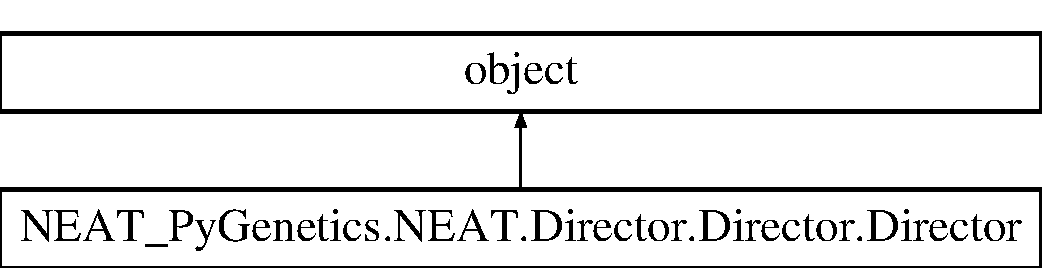
\includegraphics[height=2.000000cm]{classNEAT__PyGenetics_1_1NEAT_1_1Director_1_1Director_1_1Director}
\end{center}
\end{figure}
\subsection*{Public Member Functions}
\begin{DoxyCompactItemize}
\item 
def \hyperlink{classNEAT__PyGenetics_1_1NEAT_1_1Director_1_1Director_1_1Director_a2e4d16b66d8b60ec696d3c734a7e5833}{run} (self)
\end{DoxyCompactItemize}


\subsection{Member Function Documentation}
\index{N\+E\+A\+T\+\_\+\+Py\+Genetics\+::\+N\+E\+A\+T\+::\+Director\+::\+Director\+::\+Director@{N\+E\+A\+T\+\_\+\+Py\+Genetics\+::\+N\+E\+A\+T\+::\+Director\+::\+Director\+::\+Director}!run@{run}}
\index{run@{run}!N\+E\+A\+T\+\_\+\+Py\+Genetics\+::\+N\+E\+A\+T\+::\+Director\+::\+Director\+::\+Director@{N\+E\+A\+T\+\_\+\+Py\+Genetics\+::\+N\+E\+A\+T\+::\+Director\+::\+Director\+::\+Director}}
\subsubsection[{\texorpdfstring{run(self)}{run(self)}}]{\setlength{\rightskip}{0pt plus 5cm}def N\+E\+A\+T\+\_\+\+Py\+Genetics.\+N\+E\+A\+T.\+Director.\+Director.\+Director.\+run (
\begin{DoxyParamCaption}
\item[{}]{self}
\end{DoxyParamCaption}
)}\hypertarget{classNEAT__PyGenetics_1_1NEAT_1_1Director_1_1Director_1_1Director_a2e4d16b66d8b60ec696d3c734a7e5833}{}\label{classNEAT__PyGenetics_1_1NEAT_1_1Director_1_1Director_1_1Director_a2e4d16b66d8b60ec696d3c734a7e5833}


The documentation for this class was generated from the following file\+:\begin{DoxyCompactItemize}
\item 
N\+E\+A\+T/\+Director/\hyperlink{Director_8py}{Director.\+py}\end{DoxyCompactItemize}

\hypertarget{classNEAT__PyGenetics_1_1NEAT_1_1Repository_1_1GeneRepository_1_1GeneRepository}{}\section{N\+E\+A\+T\+\_\+\+Py\+Genetics.\+N\+E\+A\+T.\+Repository.\+Gene\+Repository.\+Gene\+Repository Class Reference}
\label{classNEAT__PyGenetics_1_1NEAT_1_1Repository_1_1GeneRepository_1_1GeneRepository}\index{N\+E\+A\+T\+\_\+\+Py\+Genetics.\+N\+E\+A\+T.\+Repository.\+Gene\+Repository.\+Gene\+Repository@{N\+E\+A\+T\+\_\+\+Py\+Genetics.\+N\+E\+A\+T.\+Repository.\+Gene\+Repository.\+Gene\+Repository}}
Inheritance diagram for N\+E\+A\+T\+\_\+\+Py\+Genetics.\+N\+E\+A\+T.\+Repository.\+Gene\+Repository.\+Gene\+Repository\+:\begin{figure}[H]
\begin{center}
\leavevmode
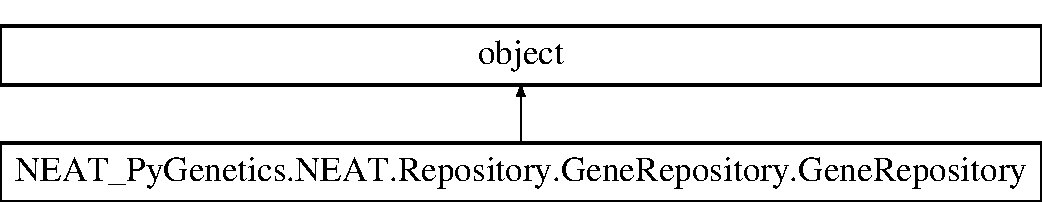
\includegraphics[height=2.000000cm]{classNEAT__PyGenetics_1_1NEAT_1_1Repository_1_1GeneRepository_1_1GeneRepository}
\end{center}
\end{figure}
\subsection*{Public Member Functions}
\begin{DoxyCompactItemize}
\item 
def \hyperlink{classNEAT__PyGenetics_1_1NEAT_1_1Repository_1_1GeneRepository_1_1GeneRepository_a47867f001b69fb1af342bd56077eb2d1}{\+\_\+\+\_\+init\+\_\+\+\_\+}
\item 
def \hyperlink{classNEAT__PyGenetics_1_1NEAT_1_1Repository_1_1GeneRepository_1_1GeneRepository_acf117ca8d8fb85263ab1e419e795bc3f}{get\+\_\+gene\+\_\+id\+\_\+for\+\_\+endpoints} (self, head\+\_\+node\+\_\+id, tail\+\_\+node\+\_\+id)
\item 
def \hyperlink{classNEAT__PyGenetics_1_1NEAT_1_1Repository_1_1GeneRepository_1_1GeneRepository_a12b448287c1e00d71325a0f4f5191b0b}{find\+\_\+connecting\+\_\+nodes} (self, head\+\_\+node\+\_\+id, tail\+\_\+node\+\_\+id)
\item 
def \hyperlink{classNEAT__PyGenetics_1_1NEAT_1_1Repository_1_1GeneRepository_1_1GeneRepository_a1cf66c6d6fbb68a38a5915ccfbab77cb}{get\+\_\+next\+\_\+node\+\_\+label} (self)
\item 
def \hyperlink{classNEAT__PyGenetics_1_1NEAT_1_1Repository_1_1GeneRepository_1_1GeneRepository_a135cdf881aca932199a40ace71aa88e2}{get\+\_\+node\+\_\+labels\+\_\+by\+\_\+gene\+\_\+id} (self, gene\+\_\+id)
\end{DoxyCompactItemize}


\subsection{Constructor \& Destructor Documentation}
\index{N\+E\+A\+T\+\_\+\+Py\+Genetics\+::\+N\+E\+A\+T\+::\+Repository\+::\+Gene\+Repository\+::\+Gene\+Repository@{N\+E\+A\+T\+\_\+\+Py\+Genetics\+::\+N\+E\+A\+T\+::\+Repository\+::\+Gene\+Repository\+::\+Gene\+Repository}!\+\_\+\+\_\+init\+\_\+\+\_\+@{\+\_\+\+\_\+init\+\_\+\+\_\+}}
\index{\+\_\+\+\_\+init\+\_\+\+\_\+@{\+\_\+\+\_\+init\+\_\+\+\_\+}!N\+E\+A\+T\+\_\+\+Py\+Genetics\+::\+N\+E\+A\+T\+::\+Repository\+::\+Gene\+Repository\+::\+Gene\+Repository@{N\+E\+A\+T\+\_\+\+Py\+Genetics\+::\+N\+E\+A\+T\+::\+Repository\+::\+Gene\+Repository\+::\+Gene\+Repository}}
\subsubsection[{\texorpdfstring{\+\_\+\+\_\+init\+\_\+\+\_\+}{__init__}}]{\setlength{\rightskip}{0pt plus 5cm}def N\+E\+A\+T\+\_\+\+Py\+Genetics.\+N\+E\+A\+T.\+Repository.\+Gene\+Repository.\+Gene\+Repository.\+\_\+\+\_\+init\+\_\+\+\_\+ (
\begin{DoxyParamCaption}
\item[{}]{self, }
\item[{}]{database\+\_\+connector}
\end{DoxyParamCaption}
)}\hypertarget{classNEAT__PyGenetics_1_1NEAT_1_1Repository_1_1GeneRepository_1_1GeneRepository_a47867f001b69fb1af342bd56077eb2d1}{}\label{classNEAT__PyGenetics_1_1NEAT_1_1Repository_1_1GeneRepository_1_1GeneRepository_a47867f001b69fb1af342bd56077eb2d1}


\subsection{Member Function Documentation}
\index{N\+E\+A\+T\+\_\+\+Py\+Genetics\+::\+N\+E\+A\+T\+::\+Repository\+::\+Gene\+Repository\+::\+Gene\+Repository@{N\+E\+A\+T\+\_\+\+Py\+Genetics\+::\+N\+E\+A\+T\+::\+Repository\+::\+Gene\+Repository\+::\+Gene\+Repository}!find\+\_\+connecting\+\_\+nodes@{find\+\_\+connecting\+\_\+nodes}}
\index{find\+\_\+connecting\+\_\+nodes@{find\+\_\+connecting\+\_\+nodes}!N\+E\+A\+T\+\_\+\+Py\+Genetics\+::\+N\+E\+A\+T\+::\+Repository\+::\+Gene\+Repository\+::\+Gene\+Repository@{N\+E\+A\+T\+\_\+\+Py\+Genetics\+::\+N\+E\+A\+T\+::\+Repository\+::\+Gene\+Repository\+::\+Gene\+Repository}}
\subsubsection[{\texorpdfstring{find\+\_\+connecting\+\_\+nodes(self, head\+\_\+node\+\_\+id, tail\+\_\+node\+\_\+id)}{find_connecting_nodes(self, head_node_id, tail_node_id)}}]{\setlength{\rightskip}{0pt plus 5cm}def N\+E\+A\+T\+\_\+\+Py\+Genetics.\+N\+E\+A\+T.\+Repository.\+Gene\+Repository.\+Gene\+Repository.\+find\+\_\+connecting\+\_\+nodes (
\begin{DoxyParamCaption}
\item[{}]{self, }
\item[{}]{head\+\_\+node\+\_\+id, }
\item[{}]{tail\+\_\+node\+\_\+id}
\end{DoxyParamCaption}
)}\hypertarget{classNEAT__PyGenetics_1_1NEAT_1_1Repository_1_1GeneRepository_1_1GeneRepository_a12b448287c1e00d71325a0f4f5191b0b}{}\label{classNEAT__PyGenetics_1_1NEAT_1_1Repository_1_1GeneRepository_1_1GeneRepository_a12b448287c1e00d71325a0f4f5191b0b}
\index{N\+E\+A\+T\+\_\+\+Py\+Genetics\+::\+N\+E\+A\+T\+::\+Repository\+::\+Gene\+Repository\+::\+Gene\+Repository@{N\+E\+A\+T\+\_\+\+Py\+Genetics\+::\+N\+E\+A\+T\+::\+Repository\+::\+Gene\+Repository\+::\+Gene\+Repository}!get\+\_\+gene\+\_\+id\+\_\+for\+\_\+endpoints@{get\+\_\+gene\+\_\+id\+\_\+for\+\_\+endpoints}}
\index{get\+\_\+gene\+\_\+id\+\_\+for\+\_\+endpoints@{get\+\_\+gene\+\_\+id\+\_\+for\+\_\+endpoints}!N\+E\+A\+T\+\_\+\+Py\+Genetics\+::\+N\+E\+A\+T\+::\+Repository\+::\+Gene\+Repository\+::\+Gene\+Repository@{N\+E\+A\+T\+\_\+\+Py\+Genetics\+::\+N\+E\+A\+T\+::\+Repository\+::\+Gene\+Repository\+::\+Gene\+Repository}}
\subsubsection[{\texorpdfstring{get\+\_\+gene\+\_\+id\+\_\+for\+\_\+endpoints(self, head\+\_\+node\+\_\+id, tail\+\_\+node\+\_\+id)}{get_gene_id_for_endpoints(self, head_node_id, tail_node_id)}}]{\setlength{\rightskip}{0pt plus 5cm}def N\+E\+A\+T\+\_\+\+Py\+Genetics.\+N\+E\+A\+T.\+Repository.\+Gene\+Repository.\+Gene\+Repository.\+get\+\_\+gene\+\_\+id\+\_\+for\+\_\+endpoints (
\begin{DoxyParamCaption}
\item[{}]{self, }
\item[{}]{head\+\_\+node\+\_\+id, }
\item[{}]{tail\+\_\+node\+\_\+id}
\end{DoxyParamCaption}
)}\hypertarget{classNEAT__PyGenetics_1_1NEAT_1_1Repository_1_1GeneRepository_1_1GeneRepository_acf117ca8d8fb85263ab1e419e795bc3f}{}\label{classNEAT__PyGenetics_1_1NEAT_1_1Repository_1_1GeneRepository_1_1GeneRepository_acf117ca8d8fb85263ab1e419e795bc3f}
\index{N\+E\+A\+T\+\_\+\+Py\+Genetics\+::\+N\+E\+A\+T\+::\+Repository\+::\+Gene\+Repository\+::\+Gene\+Repository@{N\+E\+A\+T\+\_\+\+Py\+Genetics\+::\+N\+E\+A\+T\+::\+Repository\+::\+Gene\+Repository\+::\+Gene\+Repository}!get\+\_\+next\+\_\+node\+\_\+label@{get\+\_\+next\+\_\+node\+\_\+label}}
\index{get\+\_\+next\+\_\+node\+\_\+label@{get\+\_\+next\+\_\+node\+\_\+label}!N\+E\+A\+T\+\_\+\+Py\+Genetics\+::\+N\+E\+A\+T\+::\+Repository\+::\+Gene\+Repository\+::\+Gene\+Repository@{N\+E\+A\+T\+\_\+\+Py\+Genetics\+::\+N\+E\+A\+T\+::\+Repository\+::\+Gene\+Repository\+::\+Gene\+Repository}}
\subsubsection[{\texorpdfstring{get\+\_\+next\+\_\+node\+\_\+label(self)}{get_next_node_label(self)}}]{\setlength{\rightskip}{0pt plus 5cm}def N\+E\+A\+T\+\_\+\+Py\+Genetics.\+N\+E\+A\+T.\+Repository.\+Gene\+Repository.\+Gene\+Repository.\+get\+\_\+next\+\_\+node\+\_\+label (
\begin{DoxyParamCaption}
\item[{}]{self}
\end{DoxyParamCaption}
)}\hypertarget{classNEAT__PyGenetics_1_1NEAT_1_1Repository_1_1GeneRepository_1_1GeneRepository_a1cf66c6d6fbb68a38a5915ccfbab77cb}{}\label{classNEAT__PyGenetics_1_1NEAT_1_1Repository_1_1GeneRepository_1_1GeneRepository_a1cf66c6d6fbb68a38a5915ccfbab77cb}
\index{N\+E\+A\+T\+\_\+\+Py\+Genetics\+::\+N\+E\+A\+T\+::\+Repository\+::\+Gene\+Repository\+::\+Gene\+Repository@{N\+E\+A\+T\+\_\+\+Py\+Genetics\+::\+N\+E\+A\+T\+::\+Repository\+::\+Gene\+Repository\+::\+Gene\+Repository}!get\+\_\+node\+\_\+labels\+\_\+by\+\_\+gene\+\_\+id@{get\+\_\+node\+\_\+labels\+\_\+by\+\_\+gene\+\_\+id}}
\index{get\+\_\+node\+\_\+labels\+\_\+by\+\_\+gene\+\_\+id@{get\+\_\+node\+\_\+labels\+\_\+by\+\_\+gene\+\_\+id}!N\+E\+A\+T\+\_\+\+Py\+Genetics\+::\+N\+E\+A\+T\+::\+Repository\+::\+Gene\+Repository\+::\+Gene\+Repository@{N\+E\+A\+T\+\_\+\+Py\+Genetics\+::\+N\+E\+A\+T\+::\+Repository\+::\+Gene\+Repository\+::\+Gene\+Repository}}
\subsubsection[{\texorpdfstring{get\+\_\+node\+\_\+labels\+\_\+by\+\_\+gene\+\_\+id(self, gene\+\_\+id)}{get_node_labels_by_gene_id(self, gene_id)}}]{\setlength{\rightskip}{0pt plus 5cm}def N\+E\+A\+T\+\_\+\+Py\+Genetics.\+N\+E\+A\+T.\+Repository.\+Gene\+Repository.\+Gene\+Repository.\+get\+\_\+node\+\_\+labels\+\_\+by\+\_\+gene\+\_\+id (
\begin{DoxyParamCaption}
\item[{}]{self, }
\item[{}]{gene\+\_\+id}
\end{DoxyParamCaption}
)}\hypertarget{classNEAT__PyGenetics_1_1NEAT_1_1Repository_1_1GeneRepository_1_1GeneRepository_a135cdf881aca932199a40ace71aa88e2}{}\label{classNEAT__PyGenetics_1_1NEAT_1_1Repository_1_1GeneRepository_1_1GeneRepository_a135cdf881aca932199a40ace71aa88e2}


The documentation for this class was generated from the following file\+:\begin{DoxyCompactItemize}
\item 
N\+E\+A\+T/\+Repository/\hyperlink{GeneRepository_8py}{Gene\+Repository.\+py}\end{DoxyCompactItemize}

\hypertarget{classNEAT__PyGenetics_1_1NEAT_1_1Analyst_1_1GenomeAnalyst_1_1GenomeAnalyst}{}\section{N\+E\+A\+T\+\_\+\+Py\+Genetics.\+N\+E\+A\+T.\+Analyst.\+Genome\+Analyst.\+Genome\+Analyst Class Reference}
\label{classNEAT__PyGenetics_1_1NEAT_1_1Analyst_1_1GenomeAnalyst_1_1GenomeAnalyst}\index{N\+E\+A\+T\+\_\+\+Py\+Genetics.\+N\+E\+A\+T.\+Analyst.\+Genome\+Analyst.\+Genome\+Analyst@{N\+E\+A\+T\+\_\+\+Py\+Genetics.\+N\+E\+A\+T.\+Analyst.\+Genome\+Analyst.\+Genome\+Analyst}}
Inheritance diagram for N\+E\+A\+T\+\_\+\+Py\+Genetics.\+N\+E\+A\+T.\+Analyst.\+Genome\+Analyst.\+Genome\+Analyst\+:\begin{figure}[H]
\begin{center}
\leavevmode
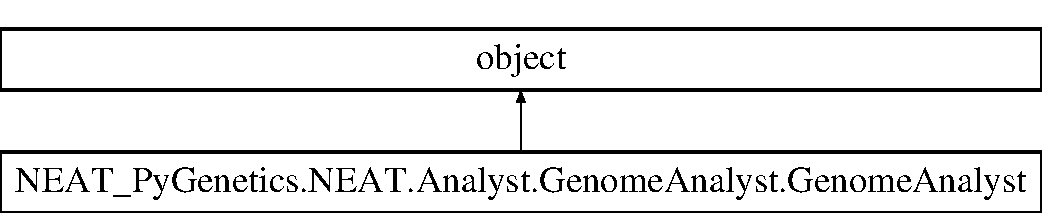
\includegraphics[height=2.000000cm]{classNEAT__PyGenetics_1_1NEAT_1_1Analyst_1_1GenomeAnalyst_1_1GenomeAnalyst}
\end{center}
\end{figure}
\subsection*{Public Member Functions}
\begin{DoxyCompactItemize}
\item 
def \hyperlink{classNEAT__PyGenetics_1_1NEAT_1_1Analyst_1_1GenomeAnalyst_1_1GenomeAnalyst_a2b9e3334de517a0555177ee6bcc0ac04}{\+\_\+\+\_\+init\+\_\+\+\_\+} (self)
\begin{DoxyCompactList}\small\item\em \+\_\+node\+\_\+visited\+: \+\_\+node\+\_\+visited\mbox{[}i\mbox{]} = 0 =$>$ node with id i was not visited yet \+\_\+node\+\_\+visited\mbox{[}i\mbox{]} = 1 =$>$ node with id i was visited \+:return\+: \end{DoxyCompactList}\item 
def \hyperlink{classNEAT__PyGenetics_1_1NEAT_1_1Analyst_1_1GenomeAnalyst_1_1GenomeAnalyst_afdd3b4e6b0b8275dd62677b8d5a18933}{analyze}
\begin{DoxyCompactList}\small\item\em Analysis method. \end{DoxyCompactList}\end{DoxyCompactItemize}
\subsection*{Static Public Attributes}
\begin{DoxyCompactItemize}
\item 
\hyperlink{classNEAT__PyGenetics_1_1NEAT_1_1Analyst_1_1GenomeAnalyst_1_1GenomeAnalyst_a61333814f998f2c80d271f3ebc92d198}{topologically\+\_\+sorted\+\_\+nodes}
\item 
\hyperlink{classNEAT__PyGenetics_1_1NEAT_1_1Analyst_1_1GenomeAnalyst_1_1GenomeAnalyst_a5453383e771c7f655739ee80508a8b08}{cycle\+\_\+edges}
\item 
\hyperlink{classNEAT__PyGenetics_1_1NEAT_1_1Analyst_1_1GenomeAnalyst_1_1GenomeAnalyst_adee62c855c0445f8b5c4032ceaf1217d}{topologically\+\_\+sorted\+\_\+cycle\+\_\+nodes}
\end{DoxyCompactItemize}


\subsection{Constructor \& Destructor Documentation}
\index{N\+E\+A\+T\+\_\+\+Py\+Genetics\+::\+N\+E\+A\+T\+::\+Analyst\+::\+Genome\+Analyst\+::\+Genome\+Analyst@{N\+E\+A\+T\+\_\+\+Py\+Genetics\+::\+N\+E\+A\+T\+::\+Analyst\+::\+Genome\+Analyst\+::\+Genome\+Analyst}!\+\_\+\+\_\+init\+\_\+\+\_\+@{\+\_\+\+\_\+init\+\_\+\+\_\+}}
\index{\+\_\+\+\_\+init\+\_\+\+\_\+@{\+\_\+\+\_\+init\+\_\+\+\_\+}!N\+E\+A\+T\+\_\+\+Py\+Genetics\+::\+N\+E\+A\+T\+::\+Analyst\+::\+Genome\+Analyst\+::\+Genome\+Analyst@{N\+E\+A\+T\+\_\+\+Py\+Genetics\+::\+N\+E\+A\+T\+::\+Analyst\+::\+Genome\+Analyst\+::\+Genome\+Analyst}}
\subsubsection[{\texorpdfstring{\+\_\+\+\_\+init\+\_\+\+\_\+(self)}{__init__(self)}}]{\setlength{\rightskip}{0pt plus 5cm}def N\+E\+A\+T\+\_\+\+Py\+Genetics.\+N\+E\+A\+T.\+Analyst.\+Genome\+Analyst.\+Genome\+Analyst.\+\_\+\+\_\+init\+\_\+\+\_\+ (
\begin{DoxyParamCaption}
\item[{}]{self}
\end{DoxyParamCaption}
)}\hypertarget{classNEAT__PyGenetics_1_1NEAT_1_1Analyst_1_1GenomeAnalyst_1_1GenomeAnalyst_a2b9e3334de517a0555177ee6bcc0ac04}{}\label{classNEAT__PyGenetics_1_1NEAT_1_1Analyst_1_1GenomeAnalyst_1_1GenomeAnalyst_a2b9e3334de517a0555177ee6bcc0ac04}


\+\_\+node\+\_\+visited\+: \+\_\+node\+\_\+visited\mbox{[}i\mbox{]} = 0 =$>$ node with id i was not visited yet \+\_\+node\+\_\+visited\mbox{[}i\mbox{]} = 1 =$>$ node with id i was visited \+:return\+: 



\subsection{Member Function Documentation}
\index{N\+E\+A\+T\+\_\+\+Py\+Genetics\+::\+N\+E\+A\+T\+::\+Analyst\+::\+Genome\+Analyst\+::\+Genome\+Analyst@{N\+E\+A\+T\+\_\+\+Py\+Genetics\+::\+N\+E\+A\+T\+::\+Analyst\+::\+Genome\+Analyst\+::\+Genome\+Analyst}!analyze@{analyze}}
\index{analyze@{analyze}!N\+E\+A\+T\+\_\+\+Py\+Genetics\+::\+N\+E\+A\+T\+::\+Analyst\+::\+Genome\+Analyst\+::\+Genome\+Analyst@{N\+E\+A\+T\+\_\+\+Py\+Genetics\+::\+N\+E\+A\+T\+::\+Analyst\+::\+Genome\+Analyst\+::\+Genome\+Analyst}}
\subsubsection[{\texorpdfstring{analyze}{analyze}}]{\setlength{\rightskip}{0pt plus 5cm}def N\+E\+A\+T\+\_\+\+Py\+Genetics.\+N\+E\+A\+T.\+Analyst.\+Genome\+Analyst.\+Genome\+Analyst.\+analyze (
\begin{DoxyParamCaption}
\item[{}]{self, }
\item[{}]{genome}
\end{DoxyParamCaption}
)}\hypertarget{classNEAT__PyGenetics_1_1NEAT_1_1Analyst_1_1GenomeAnalyst_1_1GenomeAnalyst_afdd3b4e6b0b8275dd62677b8d5a18933}{}\label{classNEAT__PyGenetics_1_1NEAT_1_1Analyst_1_1GenomeAnalyst_1_1GenomeAnalyst_afdd3b4e6b0b8275dd62677b8d5a18933}


Analysis method. 

Runs depth first search on the graph in order to find cycles and sort the graph topologically. Creates an \hyperlink{namespaceNEAT__PyGenetics_1_1NEAT_1_1Analyst_1_1AnalysisResult}{Analysis\+Result} object which can be accessed through Analysis\+Genome.\+result.

\+:param genome\+: \+:return\+: None 

\subsection{Member Data Documentation}
\index{N\+E\+A\+T\+\_\+\+Py\+Genetics\+::\+N\+E\+A\+T\+::\+Analyst\+::\+Genome\+Analyst\+::\+Genome\+Analyst@{N\+E\+A\+T\+\_\+\+Py\+Genetics\+::\+N\+E\+A\+T\+::\+Analyst\+::\+Genome\+Analyst\+::\+Genome\+Analyst}!cycle\+\_\+edges@{cycle\+\_\+edges}}
\index{cycle\+\_\+edges@{cycle\+\_\+edges}!N\+E\+A\+T\+\_\+\+Py\+Genetics\+::\+N\+E\+A\+T\+::\+Analyst\+::\+Genome\+Analyst\+::\+Genome\+Analyst@{N\+E\+A\+T\+\_\+\+Py\+Genetics\+::\+N\+E\+A\+T\+::\+Analyst\+::\+Genome\+Analyst\+::\+Genome\+Analyst}}
\subsubsection[{\texorpdfstring{cycle\+\_\+edges}{cycle_edges}}]{\setlength{\rightskip}{0pt plus 5cm}N\+E\+A\+T\+\_\+\+Py\+Genetics.\+N\+E\+A\+T.\+Analyst.\+Genome\+Analyst.\+Genome\+Analyst.\+cycle\+\_\+edges\hspace{0.3cm}{\ttfamily [static]}}\hypertarget{classNEAT__PyGenetics_1_1NEAT_1_1Analyst_1_1GenomeAnalyst_1_1GenomeAnalyst_a5453383e771c7f655739ee80508a8b08}{}\label{classNEAT__PyGenetics_1_1NEAT_1_1Analyst_1_1GenomeAnalyst_1_1GenomeAnalyst_a5453383e771c7f655739ee80508a8b08}
\index{N\+E\+A\+T\+\_\+\+Py\+Genetics\+::\+N\+E\+A\+T\+::\+Analyst\+::\+Genome\+Analyst\+::\+Genome\+Analyst@{N\+E\+A\+T\+\_\+\+Py\+Genetics\+::\+N\+E\+A\+T\+::\+Analyst\+::\+Genome\+Analyst\+::\+Genome\+Analyst}!topologically\+\_\+sorted\+\_\+cycle\+\_\+nodes@{topologically\+\_\+sorted\+\_\+cycle\+\_\+nodes}}
\index{topologically\+\_\+sorted\+\_\+cycle\+\_\+nodes@{topologically\+\_\+sorted\+\_\+cycle\+\_\+nodes}!N\+E\+A\+T\+\_\+\+Py\+Genetics\+::\+N\+E\+A\+T\+::\+Analyst\+::\+Genome\+Analyst\+::\+Genome\+Analyst@{N\+E\+A\+T\+\_\+\+Py\+Genetics\+::\+N\+E\+A\+T\+::\+Analyst\+::\+Genome\+Analyst\+::\+Genome\+Analyst}}
\subsubsection[{\texorpdfstring{topologically\+\_\+sorted\+\_\+cycle\+\_\+nodes}{topologically_sorted_cycle_nodes}}]{\setlength{\rightskip}{0pt plus 5cm}N\+E\+A\+T\+\_\+\+Py\+Genetics.\+N\+E\+A\+T.\+Analyst.\+Genome\+Analyst.\+Genome\+Analyst.\+topologically\+\_\+sorted\+\_\+cycle\+\_\+nodes\hspace{0.3cm}{\ttfamily [static]}}\hypertarget{classNEAT__PyGenetics_1_1NEAT_1_1Analyst_1_1GenomeAnalyst_1_1GenomeAnalyst_adee62c855c0445f8b5c4032ceaf1217d}{}\label{classNEAT__PyGenetics_1_1NEAT_1_1Analyst_1_1GenomeAnalyst_1_1GenomeAnalyst_adee62c855c0445f8b5c4032ceaf1217d}
\index{N\+E\+A\+T\+\_\+\+Py\+Genetics\+::\+N\+E\+A\+T\+::\+Analyst\+::\+Genome\+Analyst\+::\+Genome\+Analyst@{N\+E\+A\+T\+\_\+\+Py\+Genetics\+::\+N\+E\+A\+T\+::\+Analyst\+::\+Genome\+Analyst\+::\+Genome\+Analyst}!topologically\+\_\+sorted\+\_\+nodes@{topologically\+\_\+sorted\+\_\+nodes}}
\index{topologically\+\_\+sorted\+\_\+nodes@{topologically\+\_\+sorted\+\_\+nodes}!N\+E\+A\+T\+\_\+\+Py\+Genetics\+::\+N\+E\+A\+T\+::\+Analyst\+::\+Genome\+Analyst\+::\+Genome\+Analyst@{N\+E\+A\+T\+\_\+\+Py\+Genetics\+::\+N\+E\+A\+T\+::\+Analyst\+::\+Genome\+Analyst\+::\+Genome\+Analyst}}
\subsubsection[{\texorpdfstring{topologically\+\_\+sorted\+\_\+nodes}{topologically_sorted_nodes}}]{\setlength{\rightskip}{0pt plus 5cm}N\+E\+A\+T\+\_\+\+Py\+Genetics.\+N\+E\+A\+T.\+Analyst.\+Genome\+Analyst.\+Genome\+Analyst.\+topologically\+\_\+sorted\+\_\+nodes\hspace{0.3cm}{\ttfamily [static]}}\hypertarget{classNEAT__PyGenetics_1_1NEAT_1_1Analyst_1_1GenomeAnalyst_1_1GenomeAnalyst_a61333814f998f2c80d271f3ebc92d198}{}\label{classNEAT__PyGenetics_1_1NEAT_1_1Analyst_1_1GenomeAnalyst_1_1GenomeAnalyst_a61333814f998f2c80d271f3ebc92d198}


The documentation for this class was generated from the following file\+:\begin{DoxyCompactItemize}
\item 
N\+E\+A\+T/\+Analyst/\hyperlink{GenomeAnalyst_8py}{Genome\+Analyst.\+py}\end{DoxyCompactItemize}

\hypertarget{classNEAT__PyGenetics_1_1NEAT_1_1Analyst_1_1GenomeClusterer_1_1GenomeClusterer}{}\section{N\+E\+A\+T\+\_\+\+Py\+Genetics.\+N\+E\+A\+T.\+Analyst.\+Genome\+Clusterer.\+Genome\+Clusterer Class Reference}
\label{classNEAT__PyGenetics_1_1NEAT_1_1Analyst_1_1GenomeClusterer_1_1GenomeClusterer}\index{N\+E\+A\+T\+\_\+\+Py\+Genetics.\+N\+E\+A\+T.\+Analyst.\+Genome\+Clusterer.\+Genome\+Clusterer@{N\+E\+A\+T\+\_\+\+Py\+Genetics.\+N\+E\+A\+T.\+Analyst.\+Genome\+Clusterer.\+Genome\+Clusterer}}


A class used for clustering genomes into species.  


Inheritance diagram for N\+E\+A\+T\+\_\+\+Py\+Genetics.\+N\+E\+A\+T.\+Analyst.\+Genome\+Clusterer.\+Genome\+Clusterer\+:\begin{figure}[H]
\begin{center}
\leavevmode
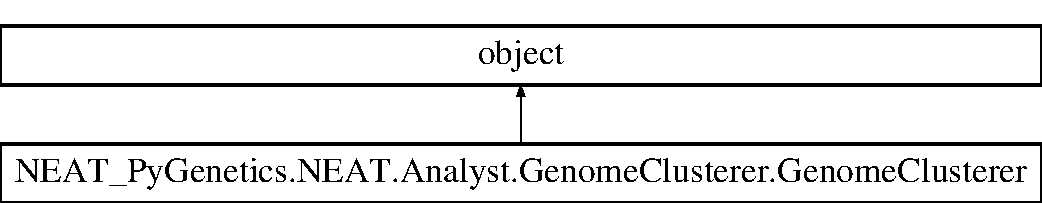
\includegraphics[height=2.000000cm]{classNEAT__PyGenetics_1_1NEAT_1_1Analyst_1_1GenomeClusterer_1_1GenomeClusterer}
\end{center}
\end{figure}
\subsection*{Public Member Functions}
\begin{DoxyCompactItemize}
\item 
def \hyperlink{classNEAT__PyGenetics_1_1NEAT_1_1Analyst_1_1GenomeClusterer_1_1GenomeClusterer_a2f18f1f814c59bc18bc896c67331db10}{\+\_\+\+\_\+init\+\_\+\+\_\+}
\item 
def \hyperlink{classNEAT__PyGenetics_1_1NEAT_1_1Analyst_1_1GenomeClusterer_1_1GenomeClusterer_a3cb27bd4e57fbae51f5638bf252d7d19}{cluster\+\_\+genomes}
\item 
def \hyperlink{classNEAT__PyGenetics_1_1NEAT_1_1Analyst_1_1GenomeClusterer_1_1GenomeClusterer_a4b17098e6b96981aa7a00ffe3c3510c8}{cluster\+\_\+genome}
\item 
def \hyperlink{classNEAT__PyGenetics_1_1NEAT_1_1Analyst_1_1GenomeClusterer_1_1GenomeClusterer_a057cec399fba67f9f90c70ad9158ec5e}{calculate\+\_\+delta}
\item 
def \hyperlink{classNEAT__PyGenetics_1_1NEAT_1_1Analyst_1_1GenomeClusterer_1_1GenomeClusterer_a5dba985534b3de86bb03574e683749f6}{calculate\+\_\+cluster\+\_\+fitness}
\item 
def \hyperlink{classNEAT__PyGenetics_1_1NEAT_1_1Analyst_1_1GenomeClusterer_1_1GenomeClusterer_a6bd0107d083dade08414c19ad9aaadaf}{calculate\+\_\+cluster\+\_\+offspring\+\_\+values} (self)
\end{DoxyCompactItemize}
\subsection*{Static Public Member Functions}
\begin{DoxyCompactItemize}
\item 
def \hyperlink{classNEAT__PyGenetics_1_1NEAT_1_1Analyst_1_1GenomeClusterer_1_1GenomeClusterer_a25f21d57d135bbf3b0f23bbfdef375e7}{calculate\+\_\+disjoint\+\_\+excess\+\_\+count}
\item 
def \hyperlink{classNEAT__PyGenetics_1_1NEAT_1_1Analyst_1_1GenomeClusterer_1_1GenomeClusterer_a748db217e8ce0c9f3e4302b00b4677e8}{calculate\+\_\+average\+\_\+weight\+\_\+difference}
\end{DoxyCompactItemize}
\subsection*{Static Public Attributes}
\begin{DoxyCompactItemize}
\item 
\hyperlink{classNEAT__PyGenetics_1_1NEAT_1_1Analyst_1_1GenomeClusterer_1_1GenomeClusterer_af9623df2d784da3e4c186b729c63bb81}{genome\+\_\+repository}
\item 
\hyperlink{classNEAT__PyGenetics_1_1NEAT_1_1Analyst_1_1GenomeClusterer_1_1GenomeClusterer_ab9332a669c7c28ee6d33806da38eee45}{cluster\+\_\+repository}
\item 
\hyperlink{classNEAT__PyGenetics_1_1NEAT_1_1Analyst_1_1GenomeClusterer_1_1GenomeClusterer_a23498ab192f633f9bada8709832b5fed}{clustering\+\_\+parameters}
\item 
\hyperlink{classNEAT__PyGenetics_1_1NEAT_1_1Analyst_1_1GenomeClusterer_1_1GenomeClusterer_aefeaee4266e3fab9ff64f0b23fa08902}{excess\+\_\+coefficient}
\item 
\hyperlink{classNEAT__PyGenetics_1_1NEAT_1_1Analyst_1_1GenomeClusterer_1_1GenomeClusterer_a2d3a31646312ae391f5805b5f5a7c0c5}{disjoint\+\_\+coefficient}
\item 
\hyperlink{classNEAT__PyGenetics_1_1NEAT_1_1Analyst_1_1GenomeClusterer_1_1GenomeClusterer_a4d2e391563722c816e807faf0011aabf}{weight\+\_\+delta\+\_\+coefficient}
\item 
\hyperlink{classNEAT__PyGenetics_1_1NEAT_1_1Analyst_1_1GenomeClusterer_1_1GenomeClusterer_a5b2d70ae35a4051f4663c496190f0780}{bigger\+\_\+genome}
\item 
\hyperlink{classNEAT__PyGenetics_1_1NEAT_1_1Analyst_1_1GenomeClusterer_1_1GenomeClusterer_a5b0b90cb5b44c29ae3a062a9f591cee9}{smaller\+\_\+genome}
\item 
\hyperlink{classNEAT__PyGenetics_1_1NEAT_1_1Analyst_1_1GenomeClusterer_1_1GenomeClusterer_a3046dce6838bbf4b7209358ca3c88a2a}{bigger\+\_\+genome\+\_\+gene\+\_\+ids}
\item 
\hyperlink{classNEAT__PyGenetics_1_1NEAT_1_1Analyst_1_1GenomeClusterer_1_1GenomeClusterer_ac6b59f46ec08ad39bb46b6597591ab6f}{smaller\+\_\+genome\+\_\+gene\+\_\+ids}
\item 
\hyperlink{classNEAT__PyGenetics_1_1NEAT_1_1Analyst_1_1GenomeClusterer_1_1GenomeClusterer_a73179831aa538106f4b8d7dcb54c82c7}{all\+\_\+gene\+\_\+ids}
\item 
\hyperlink{classNEAT__PyGenetics_1_1NEAT_1_1Analyst_1_1GenomeClusterer_1_1GenomeClusterer_a47fed7fbdbd9d079e693921bc38e5f3e}{matching\+\_\+genes}
\item 
\hyperlink{classNEAT__PyGenetics_1_1NEAT_1_1Analyst_1_1GenomeClusterer_1_1GenomeClusterer_a7b7e2e57ffced7bd6a6c884aa20f313a}{differing\+\_\+genes}
\item 
\hyperlink{classNEAT__PyGenetics_1_1NEAT_1_1Analyst_1_1GenomeClusterer_1_1GenomeClusterer_aed8ff1fe75594eae5a5422965cca13b5}{n}
\item 
\hyperlink{classNEAT__PyGenetics_1_1NEAT_1_1Analyst_1_1GenomeClusterer_1_1GenomeClusterer_abc33fd75cd1bbcb72c3bfea41db56b63}{disjoint\+\_\+count}
\item 
\hyperlink{classNEAT__PyGenetics_1_1NEAT_1_1Analyst_1_1GenomeClusterer_1_1GenomeClusterer_a0e1ff1aa859082568b6b5efeeb029234}{excess\+\_\+count}
\item 
\hyperlink{classNEAT__PyGenetics_1_1NEAT_1_1Analyst_1_1GenomeClusterer_1_1GenomeClusterer_adf2a23e3ff4eca53b7b4834cd9b51275}{w\+\_\+bar}
\item 
\hyperlink{classNEAT__PyGenetics_1_1NEAT_1_1Analyst_1_1GenomeClusterer_1_1GenomeClusterer_a402e6e20884053cc0ae8f04f86734091}{smaller\+\_\+genome\+\_\+range}
\item 
\hyperlink{classNEAT__PyGenetics_1_1NEAT_1_1Analyst_1_1GenomeClusterer_1_1GenomeClusterer_a4fdea1cdff3d733af9de249641892695}{excess\+\_\+genes}
\item 
\hyperlink{classNEAT__PyGenetics_1_1NEAT_1_1Analyst_1_1GenomeClusterer_1_1GenomeClusterer_a1aed67ecb6dba5bad3cf73de3b756b91}{disjoint\+\_\+genes}
\item 
\hyperlink{classNEAT__PyGenetics_1_1NEAT_1_1Analyst_1_1GenomeClusterer_1_1GenomeClusterer_aff7fba61d7cd8eeeed9149ed48211699}{weights}
\item 
\hyperlink{classNEAT__PyGenetics_1_1NEAT_1_1Analyst_1_1GenomeClusterer_1_1GenomeClusterer_ac1f8f1740d1a6663cc8fb29fe29f3c35}{weight\+\_\+one}
\item 
\hyperlink{classNEAT__PyGenetics_1_1NEAT_1_1Analyst_1_1GenomeClusterer_1_1GenomeClusterer_a2541d20300efb0cff96a18abb6a85d81}{weight\+\_\+two}
\end{DoxyCompactItemize}


\subsection{Detailed Description}
A class used for clustering genomes into species. 

\subsection{Constructor \& Destructor Documentation}
\index{N\+E\+A\+T\+\_\+\+Py\+Genetics\+::\+N\+E\+A\+T\+::\+Analyst\+::\+Genome\+Clusterer\+::\+Genome\+Clusterer@{N\+E\+A\+T\+\_\+\+Py\+Genetics\+::\+N\+E\+A\+T\+::\+Analyst\+::\+Genome\+Clusterer\+::\+Genome\+Clusterer}!\+\_\+\+\_\+init\+\_\+\+\_\+@{\+\_\+\+\_\+init\+\_\+\+\_\+}}
\index{\+\_\+\+\_\+init\+\_\+\+\_\+@{\+\_\+\+\_\+init\+\_\+\+\_\+}!N\+E\+A\+T\+\_\+\+Py\+Genetics\+::\+N\+E\+A\+T\+::\+Analyst\+::\+Genome\+Clusterer\+::\+Genome\+Clusterer@{N\+E\+A\+T\+\_\+\+Py\+Genetics\+::\+N\+E\+A\+T\+::\+Analyst\+::\+Genome\+Clusterer\+::\+Genome\+Clusterer}}
\subsubsection[{\texorpdfstring{\+\_\+\+\_\+init\+\_\+\+\_\+}{__init__}}]{\setlength{\rightskip}{0pt plus 5cm}def N\+E\+A\+T\+\_\+\+Py\+Genetics.\+N\+E\+A\+T.\+Analyst.\+Genome\+Clusterer.\+Genome\+Clusterer.\+\_\+\+\_\+init\+\_\+\+\_\+ (
\begin{DoxyParamCaption}
\item[{}]{self, }
\item[{}]{genome\+\_\+repository}
\end{DoxyParamCaption}
)}\hypertarget{classNEAT__PyGenetics_1_1NEAT_1_1Analyst_1_1GenomeClusterer_1_1GenomeClusterer_a2f18f1f814c59bc18bc896c67331db10}{}\label{classNEAT__PyGenetics_1_1NEAT_1_1Analyst_1_1GenomeClusterer_1_1GenomeClusterer_a2f18f1f814c59bc18bc896c67331db10}


\subsection{Member Function Documentation}
\index{N\+E\+A\+T\+\_\+\+Py\+Genetics\+::\+N\+E\+A\+T\+::\+Analyst\+::\+Genome\+Clusterer\+::\+Genome\+Clusterer@{N\+E\+A\+T\+\_\+\+Py\+Genetics\+::\+N\+E\+A\+T\+::\+Analyst\+::\+Genome\+Clusterer\+::\+Genome\+Clusterer}!calculate\+\_\+average\+\_\+weight\+\_\+difference@{calculate\+\_\+average\+\_\+weight\+\_\+difference}}
\index{calculate\+\_\+average\+\_\+weight\+\_\+difference@{calculate\+\_\+average\+\_\+weight\+\_\+difference}!N\+E\+A\+T\+\_\+\+Py\+Genetics\+::\+N\+E\+A\+T\+::\+Analyst\+::\+Genome\+Clusterer\+::\+Genome\+Clusterer@{N\+E\+A\+T\+\_\+\+Py\+Genetics\+::\+N\+E\+A\+T\+::\+Analyst\+::\+Genome\+Clusterer\+::\+Genome\+Clusterer}}
\subsubsection[{\texorpdfstring{calculate\+\_\+average\+\_\+weight\+\_\+difference}{calculate_average_weight_difference}}]{\setlength{\rightskip}{0pt plus 5cm}def N\+E\+A\+T\+\_\+\+Py\+Genetics.\+N\+E\+A\+T.\+Analyst.\+Genome\+Clusterer.\+Genome\+Clusterer.\+calculate\+\_\+average\+\_\+weight\+\_\+difference (
\begin{DoxyParamCaption}
\item[{}]{genome\+\_\+one}
\end{DoxyParamCaption}
)\hspace{0.3cm}{\ttfamily [static]}}\hypertarget{classNEAT__PyGenetics_1_1NEAT_1_1Analyst_1_1GenomeClusterer_1_1GenomeClusterer_a748db217e8ce0c9f3e4302b00b4677e8}{}\label{classNEAT__PyGenetics_1_1NEAT_1_1Analyst_1_1GenomeClusterer_1_1GenomeClusterer_a748db217e8ce0c9f3e4302b00b4677e8}
\index{N\+E\+A\+T\+\_\+\+Py\+Genetics\+::\+N\+E\+A\+T\+::\+Analyst\+::\+Genome\+Clusterer\+::\+Genome\+Clusterer@{N\+E\+A\+T\+\_\+\+Py\+Genetics\+::\+N\+E\+A\+T\+::\+Analyst\+::\+Genome\+Clusterer\+::\+Genome\+Clusterer}!calculate\+\_\+cluster\+\_\+fitness@{calculate\+\_\+cluster\+\_\+fitness}}
\index{calculate\+\_\+cluster\+\_\+fitness@{calculate\+\_\+cluster\+\_\+fitness}!N\+E\+A\+T\+\_\+\+Py\+Genetics\+::\+N\+E\+A\+T\+::\+Analyst\+::\+Genome\+Clusterer\+::\+Genome\+Clusterer@{N\+E\+A\+T\+\_\+\+Py\+Genetics\+::\+N\+E\+A\+T\+::\+Analyst\+::\+Genome\+Clusterer\+::\+Genome\+Clusterer}}
\subsubsection[{\texorpdfstring{calculate\+\_\+cluster\+\_\+fitness}{calculate_cluster_fitness}}]{\setlength{\rightskip}{0pt plus 5cm}def N\+E\+A\+T\+\_\+\+Py\+Genetics.\+N\+E\+A\+T.\+Analyst.\+Genome\+Clusterer.\+Genome\+Clusterer.\+calculate\+\_\+cluster\+\_\+fitness (
\begin{DoxyParamCaption}
\item[{}]{self, }
\item[{}]{cluster\+\_\+id}
\end{DoxyParamCaption}
)}\hypertarget{classNEAT__PyGenetics_1_1NEAT_1_1Analyst_1_1GenomeClusterer_1_1GenomeClusterer_a5dba985534b3de86bb03574e683749f6}{}\label{classNEAT__PyGenetics_1_1NEAT_1_1Analyst_1_1GenomeClusterer_1_1GenomeClusterer_a5dba985534b3de86bb03574e683749f6}
\index{N\+E\+A\+T\+\_\+\+Py\+Genetics\+::\+N\+E\+A\+T\+::\+Analyst\+::\+Genome\+Clusterer\+::\+Genome\+Clusterer@{N\+E\+A\+T\+\_\+\+Py\+Genetics\+::\+N\+E\+A\+T\+::\+Analyst\+::\+Genome\+Clusterer\+::\+Genome\+Clusterer}!calculate\+\_\+cluster\+\_\+offspring\+\_\+values@{calculate\+\_\+cluster\+\_\+offspring\+\_\+values}}
\index{calculate\+\_\+cluster\+\_\+offspring\+\_\+values@{calculate\+\_\+cluster\+\_\+offspring\+\_\+values}!N\+E\+A\+T\+\_\+\+Py\+Genetics\+::\+N\+E\+A\+T\+::\+Analyst\+::\+Genome\+Clusterer\+::\+Genome\+Clusterer@{N\+E\+A\+T\+\_\+\+Py\+Genetics\+::\+N\+E\+A\+T\+::\+Analyst\+::\+Genome\+Clusterer\+::\+Genome\+Clusterer}}
\subsubsection[{\texorpdfstring{calculate\+\_\+cluster\+\_\+offspring\+\_\+values(self)}{calculate_cluster_offspring_values(self)}}]{\setlength{\rightskip}{0pt plus 5cm}def N\+E\+A\+T\+\_\+\+Py\+Genetics.\+N\+E\+A\+T.\+Analyst.\+Genome\+Clusterer.\+Genome\+Clusterer.\+calculate\+\_\+cluster\+\_\+offspring\+\_\+values (
\begin{DoxyParamCaption}
\item[{}]{self}
\end{DoxyParamCaption}
)}\hypertarget{classNEAT__PyGenetics_1_1NEAT_1_1Analyst_1_1GenomeClusterer_1_1GenomeClusterer_a6bd0107d083dade08414c19ad9aaadaf}{}\label{classNEAT__PyGenetics_1_1NEAT_1_1Analyst_1_1GenomeClusterer_1_1GenomeClusterer_a6bd0107d083dade08414c19ad9aaadaf}
\index{N\+E\+A\+T\+\_\+\+Py\+Genetics\+::\+N\+E\+A\+T\+::\+Analyst\+::\+Genome\+Clusterer\+::\+Genome\+Clusterer@{N\+E\+A\+T\+\_\+\+Py\+Genetics\+::\+N\+E\+A\+T\+::\+Analyst\+::\+Genome\+Clusterer\+::\+Genome\+Clusterer}!calculate\+\_\+delta@{calculate\+\_\+delta}}
\index{calculate\+\_\+delta@{calculate\+\_\+delta}!N\+E\+A\+T\+\_\+\+Py\+Genetics\+::\+N\+E\+A\+T\+::\+Analyst\+::\+Genome\+Clusterer\+::\+Genome\+Clusterer@{N\+E\+A\+T\+\_\+\+Py\+Genetics\+::\+N\+E\+A\+T\+::\+Analyst\+::\+Genome\+Clusterer\+::\+Genome\+Clusterer}}
\subsubsection[{\texorpdfstring{calculate\+\_\+delta}{calculate_delta}}]{\setlength{\rightskip}{0pt plus 5cm}def N\+E\+A\+T\+\_\+\+Py\+Genetics.\+N\+E\+A\+T.\+Analyst.\+Genome\+Clusterer.\+Genome\+Clusterer.\+calculate\+\_\+delta (
\begin{DoxyParamCaption}
\item[{}]{self, }
\item[{}]{genome\+\_\+one}
\end{DoxyParamCaption}
)}\hypertarget{classNEAT__PyGenetics_1_1NEAT_1_1Analyst_1_1GenomeClusterer_1_1GenomeClusterer_a057cec399fba67f9f90c70ad9158ec5e}{}\label{classNEAT__PyGenetics_1_1NEAT_1_1Analyst_1_1GenomeClusterer_1_1GenomeClusterer_a057cec399fba67f9f90c70ad9158ec5e}
\index{N\+E\+A\+T\+\_\+\+Py\+Genetics\+::\+N\+E\+A\+T\+::\+Analyst\+::\+Genome\+Clusterer\+::\+Genome\+Clusterer@{N\+E\+A\+T\+\_\+\+Py\+Genetics\+::\+N\+E\+A\+T\+::\+Analyst\+::\+Genome\+Clusterer\+::\+Genome\+Clusterer}!calculate\+\_\+disjoint\+\_\+excess\+\_\+count@{calculate\+\_\+disjoint\+\_\+excess\+\_\+count}}
\index{calculate\+\_\+disjoint\+\_\+excess\+\_\+count@{calculate\+\_\+disjoint\+\_\+excess\+\_\+count}!N\+E\+A\+T\+\_\+\+Py\+Genetics\+::\+N\+E\+A\+T\+::\+Analyst\+::\+Genome\+Clusterer\+::\+Genome\+Clusterer@{N\+E\+A\+T\+\_\+\+Py\+Genetics\+::\+N\+E\+A\+T\+::\+Analyst\+::\+Genome\+Clusterer\+::\+Genome\+Clusterer}}
\subsubsection[{\texorpdfstring{calculate\+\_\+disjoint\+\_\+excess\+\_\+count}{calculate_disjoint_excess_count}}]{\setlength{\rightskip}{0pt plus 5cm}def N\+E\+A\+T\+\_\+\+Py\+Genetics.\+N\+E\+A\+T.\+Analyst.\+Genome\+Clusterer.\+Genome\+Clusterer.\+calculate\+\_\+disjoint\+\_\+excess\+\_\+count (
\begin{DoxyParamCaption}
\item[{}]{smaller\+\_\+genome\+\_\+gene\+\_\+ids}
\end{DoxyParamCaption}
)\hspace{0.3cm}{\ttfamily [static]}}\hypertarget{classNEAT__PyGenetics_1_1NEAT_1_1Analyst_1_1GenomeClusterer_1_1GenomeClusterer_a25f21d57d135bbf3b0f23bbfdef375e7}{}\label{classNEAT__PyGenetics_1_1NEAT_1_1Analyst_1_1GenomeClusterer_1_1GenomeClusterer_a25f21d57d135bbf3b0f23bbfdef375e7}
\index{N\+E\+A\+T\+\_\+\+Py\+Genetics\+::\+N\+E\+A\+T\+::\+Analyst\+::\+Genome\+Clusterer\+::\+Genome\+Clusterer@{N\+E\+A\+T\+\_\+\+Py\+Genetics\+::\+N\+E\+A\+T\+::\+Analyst\+::\+Genome\+Clusterer\+::\+Genome\+Clusterer}!cluster\+\_\+genome@{cluster\+\_\+genome}}
\index{cluster\+\_\+genome@{cluster\+\_\+genome}!N\+E\+A\+T\+\_\+\+Py\+Genetics\+::\+N\+E\+A\+T\+::\+Analyst\+::\+Genome\+Clusterer\+::\+Genome\+Clusterer@{N\+E\+A\+T\+\_\+\+Py\+Genetics\+::\+N\+E\+A\+T\+::\+Analyst\+::\+Genome\+Clusterer\+::\+Genome\+Clusterer}}
\subsubsection[{\texorpdfstring{cluster\+\_\+genome}{cluster_genome}}]{\setlength{\rightskip}{0pt plus 5cm}def N\+E\+A\+T\+\_\+\+Py\+Genetics.\+N\+E\+A\+T.\+Analyst.\+Genome\+Clusterer.\+Genome\+Clusterer.\+cluster\+\_\+genome (
\begin{DoxyParamCaption}
\item[{}]{self, }
\item[{}]{genome}
\end{DoxyParamCaption}
)}\hypertarget{classNEAT__PyGenetics_1_1NEAT_1_1Analyst_1_1GenomeClusterer_1_1GenomeClusterer_a4b17098e6b96981aa7a00ffe3c3510c8}{}\label{classNEAT__PyGenetics_1_1NEAT_1_1Analyst_1_1GenomeClusterer_1_1GenomeClusterer_a4b17098e6b96981aa7a00ffe3c3510c8}
\index{N\+E\+A\+T\+\_\+\+Py\+Genetics\+::\+N\+E\+A\+T\+::\+Analyst\+::\+Genome\+Clusterer\+::\+Genome\+Clusterer@{N\+E\+A\+T\+\_\+\+Py\+Genetics\+::\+N\+E\+A\+T\+::\+Analyst\+::\+Genome\+Clusterer\+::\+Genome\+Clusterer}!cluster\+\_\+genomes@{cluster\+\_\+genomes}}
\index{cluster\+\_\+genomes@{cluster\+\_\+genomes}!N\+E\+A\+T\+\_\+\+Py\+Genetics\+::\+N\+E\+A\+T\+::\+Analyst\+::\+Genome\+Clusterer\+::\+Genome\+Clusterer@{N\+E\+A\+T\+\_\+\+Py\+Genetics\+::\+N\+E\+A\+T\+::\+Analyst\+::\+Genome\+Clusterer\+::\+Genome\+Clusterer}}
\subsubsection[{\texorpdfstring{cluster\+\_\+genomes}{cluster_genomes}}]{\setlength{\rightskip}{0pt plus 5cm}def N\+E\+A\+T\+\_\+\+Py\+Genetics.\+N\+E\+A\+T.\+Analyst.\+Genome\+Clusterer.\+Genome\+Clusterer.\+cluster\+\_\+genomes (
\begin{DoxyParamCaption}
\item[{}]{self, }
\item[{}]{genomes}
\end{DoxyParamCaption}
)}\hypertarget{classNEAT__PyGenetics_1_1NEAT_1_1Analyst_1_1GenomeClusterer_1_1GenomeClusterer_a3cb27bd4e57fbae51f5638bf252d7d19}{}\label{classNEAT__PyGenetics_1_1NEAT_1_1Analyst_1_1GenomeClusterer_1_1GenomeClusterer_a3cb27bd4e57fbae51f5638bf252d7d19}


\subsection{Member Data Documentation}
\index{N\+E\+A\+T\+\_\+\+Py\+Genetics\+::\+N\+E\+A\+T\+::\+Analyst\+::\+Genome\+Clusterer\+::\+Genome\+Clusterer@{N\+E\+A\+T\+\_\+\+Py\+Genetics\+::\+N\+E\+A\+T\+::\+Analyst\+::\+Genome\+Clusterer\+::\+Genome\+Clusterer}!all\+\_\+gene\+\_\+ids@{all\+\_\+gene\+\_\+ids}}
\index{all\+\_\+gene\+\_\+ids@{all\+\_\+gene\+\_\+ids}!N\+E\+A\+T\+\_\+\+Py\+Genetics\+::\+N\+E\+A\+T\+::\+Analyst\+::\+Genome\+Clusterer\+::\+Genome\+Clusterer@{N\+E\+A\+T\+\_\+\+Py\+Genetics\+::\+N\+E\+A\+T\+::\+Analyst\+::\+Genome\+Clusterer\+::\+Genome\+Clusterer}}
\subsubsection[{\texorpdfstring{all\+\_\+gene\+\_\+ids}{all_gene_ids}}]{\setlength{\rightskip}{0pt plus 5cm}N\+E\+A\+T\+\_\+\+Py\+Genetics.\+N\+E\+A\+T.\+Analyst.\+Genome\+Clusterer.\+Genome\+Clusterer.\+all\+\_\+gene\+\_\+ids\hspace{0.3cm}{\ttfamily [static]}}\hypertarget{classNEAT__PyGenetics_1_1NEAT_1_1Analyst_1_1GenomeClusterer_1_1GenomeClusterer_a73179831aa538106f4b8d7dcb54c82c7}{}\label{classNEAT__PyGenetics_1_1NEAT_1_1Analyst_1_1GenomeClusterer_1_1GenomeClusterer_a73179831aa538106f4b8d7dcb54c82c7}
\index{N\+E\+A\+T\+\_\+\+Py\+Genetics\+::\+N\+E\+A\+T\+::\+Analyst\+::\+Genome\+Clusterer\+::\+Genome\+Clusterer@{N\+E\+A\+T\+\_\+\+Py\+Genetics\+::\+N\+E\+A\+T\+::\+Analyst\+::\+Genome\+Clusterer\+::\+Genome\+Clusterer}!bigger\+\_\+genome@{bigger\+\_\+genome}}
\index{bigger\+\_\+genome@{bigger\+\_\+genome}!N\+E\+A\+T\+\_\+\+Py\+Genetics\+::\+N\+E\+A\+T\+::\+Analyst\+::\+Genome\+Clusterer\+::\+Genome\+Clusterer@{N\+E\+A\+T\+\_\+\+Py\+Genetics\+::\+N\+E\+A\+T\+::\+Analyst\+::\+Genome\+Clusterer\+::\+Genome\+Clusterer}}
\subsubsection[{\texorpdfstring{bigger\+\_\+genome}{bigger_genome}}]{\setlength{\rightskip}{0pt plus 5cm}N\+E\+A\+T\+\_\+\+Py\+Genetics.\+N\+E\+A\+T.\+Analyst.\+Genome\+Clusterer.\+Genome\+Clusterer.\+bigger\+\_\+genome\hspace{0.3cm}{\ttfamily [static]}}\hypertarget{classNEAT__PyGenetics_1_1NEAT_1_1Analyst_1_1GenomeClusterer_1_1GenomeClusterer_a5b2d70ae35a4051f4663c496190f0780}{}\label{classNEAT__PyGenetics_1_1NEAT_1_1Analyst_1_1GenomeClusterer_1_1GenomeClusterer_a5b2d70ae35a4051f4663c496190f0780}
\index{N\+E\+A\+T\+\_\+\+Py\+Genetics\+::\+N\+E\+A\+T\+::\+Analyst\+::\+Genome\+Clusterer\+::\+Genome\+Clusterer@{N\+E\+A\+T\+\_\+\+Py\+Genetics\+::\+N\+E\+A\+T\+::\+Analyst\+::\+Genome\+Clusterer\+::\+Genome\+Clusterer}!bigger\+\_\+genome\+\_\+gene\+\_\+ids@{bigger\+\_\+genome\+\_\+gene\+\_\+ids}}
\index{bigger\+\_\+genome\+\_\+gene\+\_\+ids@{bigger\+\_\+genome\+\_\+gene\+\_\+ids}!N\+E\+A\+T\+\_\+\+Py\+Genetics\+::\+N\+E\+A\+T\+::\+Analyst\+::\+Genome\+Clusterer\+::\+Genome\+Clusterer@{N\+E\+A\+T\+\_\+\+Py\+Genetics\+::\+N\+E\+A\+T\+::\+Analyst\+::\+Genome\+Clusterer\+::\+Genome\+Clusterer}}
\subsubsection[{\texorpdfstring{bigger\+\_\+genome\+\_\+gene\+\_\+ids}{bigger_genome_gene_ids}}]{\setlength{\rightskip}{0pt plus 5cm}N\+E\+A\+T\+\_\+\+Py\+Genetics.\+N\+E\+A\+T.\+Analyst.\+Genome\+Clusterer.\+Genome\+Clusterer.\+bigger\+\_\+genome\+\_\+gene\+\_\+ids\hspace{0.3cm}{\ttfamily [static]}}\hypertarget{classNEAT__PyGenetics_1_1NEAT_1_1Analyst_1_1GenomeClusterer_1_1GenomeClusterer_a3046dce6838bbf4b7209358ca3c88a2a}{}\label{classNEAT__PyGenetics_1_1NEAT_1_1Analyst_1_1GenomeClusterer_1_1GenomeClusterer_a3046dce6838bbf4b7209358ca3c88a2a}
\index{N\+E\+A\+T\+\_\+\+Py\+Genetics\+::\+N\+E\+A\+T\+::\+Analyst\+::\+Genome\+Clusterer\+::\+Genome\+Clusterer@{N\+E\+A\+T\+\_\+\+Py\+Genetics\+::\+N\+E\+A\+T\+::\+Analyst\+::\+Genome\+Clusterer\+::\+Genome\+Clusterer}!cluster\+\_\+repository@{cluster\+\_\+repository}}
\index{cluster\+\_\+repository@{cluster\+\_\+repository}!N\+E\+A\+T\+\_\+\+Py\+Genetics\+::\+N\+E\+A\+T\+::\+Analyst\+::\+Genome\+Clusterer\+::\+Genome\+Clusterer@{N\+E\+A\+T\+\_\+\+Py\+Genetics\+::\+N\+E\+A\+T\+::\+Analyst\+::\+Genome\+Clusterer\+::\+Genome\+Clusterer}}
\subsubsection[{\texorpdfstring{cluster\+\_\+repository}{cluster_repository}}]{\setlength{\rightskip}{0pt plus 5cm}N\+E\+A\+T\+\_\+\+Py\+Genetics.\+N\+E\+A\+T.\+Analyst.\+Genome\+Clusterer.\+Genome\+Clusterer.\+cluster\+\_\+repository\hspace{0.3cm}{\ttfamily [static]}}\hypertarget{classNEAT__PyGenetics_1_1NEAT_1_1Analyst_1_1GenomeClusterer_1_1GenomeClusterer_ab9332a669c7c28ee6d33806da38eee45}{}\label{classNEAT__PyGenetics_1_1NEAT_1_1Analyst_1_1GenomeClusterer_1_1GenomeClusterer_ab9332a669c7c28ee6d33806da38eee45}
\index{N\+E\+A\+T\+\_\+\+Py\+Genetics\+::\+N\+E\+A\+T\+::\+Analyst\+::\+Genome\+Clusterer\+::\+Genome\+Clusterer@{N\+E\+A\+T\+\_\+\+Py\+Genetics\+::\+N\+E\+A\+T\+::\+Analyst\+::\+Genome\+Clusterer\+::\+Genome\+Clusterer}!clustering\+\_\+parameters@{clustering\+\_\+parameters}}
\index{clustering\+\_\+parameters@{clustering\+\_\+parameters}!N\+E\+A\+T\+\_\+\+Py\+Genetics\+::\+N\+E\+A\+T\+::\+Analyst\+::\+Genome\+Clusterer\+::\+Genome\+Clusterer@{N\+E\+A\+T\+\_\+\+Py\+Genetics\+::\+N\+E\+A\+T\+::\+Analyst\+::\+Genome\+Clusterer\+::\+Genome\+Clusterer}}
\subsubsection[{\texorpdfstring{clustering\+\_\+parameters}{clustering_parameters}}]{\setlength{\rightskip}{0pt plus 5cm}N\+E\+A\+T\+\_\+\+Py\+Genetics.\+N\+E\+A\+T.\+Analyst.\+Genome\+Clusterer.\+Genome\+Clusterer.\+clustering\+\_\+parameters\hspace{0.3cm}{\ttfamily [static]}}\hypertarget{classNEAT__PyGenetics_1_1NEAT_1_1Analyst_1_1GenomeClusterer_1_1GenomeClusterer_a23498ab192f633f9bada8709832b5fed}{}\label{classNEAT__PyGenetics_1_1NEAT_1_1Analyst_1_1GenomeClusterer_1_1GenomeClusterer_a23498ab192f633f9bada8709832b5fed}
\index{N\+E\+A\+T\+\_\+\+Py\+Genetics\+::\+N\+E\+A\+T\+::\+Analyst\+::\+Genome\+Clusterer\+::\+Genome\+Clusterer@{N\+E\+A\+T\+\_\+\+Py\+Genetics\+::\+N\+E\+A\+T\+::\+Analyst\+::\+Genome\+Clusterer\+::\+Genome\+Clusterer}!differing\+\_\+genes@{differing\+\_\+genes}}
\index{differing\+\_\+genes@{differing\+\_\+genes}!N\+E\+A\+T\+\_\+\+Py\+Genetics\+::\+N\+E\+A\+T\+::\+Analyst\+::\+Genome\+Clusterer\+::\+Genome\+Clusterer@{N\+E\+A\+T\+\_\+\+Py\+Genetics\+::\+N\+E\+A\+T\+::\+Analyst\+::\+Genome\+Clusterer\+::\+Genome\+Clusterer}}
\subsubsection[{\texorpdfstring{differing\+\_\+genes}{differing_genes}}]{\setlength{\rightskip}{0pt plus 5cm}N\+E\+A\+T\+\_\+\+Py\+Genetics.\+N\+E\+A\+T.\+Analyst.\+Genome\+Clusterer.\+Genome\+Clusterer.\+differing\+\_\+genes\hspace{0.3cm}{\ttfamily [static]}}\hypertarget{classNEAT__PyGenetics_1_1NEAT_1_1Analyst_1_1GenomeClusterer_1_1GenomeClusterer_a7b7e2e57ffced7bd6a6c884aa20f313a}{}\label{classNEAT__PyGenetics_1_1NEAT_1_1Analyst_1_1GenomeClusterer_1_1GenomeClusterer_a7b7e2e57ffced7bd6a6c884aa20f313a}
\index{N\+E\+A\+T\+\_\+\+Py\+Genetics\+::\+N\+E\+A\+T\+::\+Analyst\+::\+Genome\+Clusterer\+::\+Genome\+Clusterer@{N\+E\+A\+T\+\_\+\+Py\+Genetics\+::\+N\+E\+A\+T\+::\+Analyst\+::\+Genome\+Clusterer\+::\+Genome\+Clusterer}!disjoint\+\_\+coefficient@{disjoint\+\_\+coefficient}}
\index{disjoint\+\_\+coefficient@{disjoint\+\_\+coefficient}!N\+E\+A\+T\+\_\+\+Py\+Genetics\+::\+N\+E\+A\+T\+::\+Analyst\+::\+Genome\+Clusterer\+::\+Genome\+Clusterer@{N\+E\+A\+T\+\_\+\+Py\+Genetics\+::\+N\+E\+A\+T\+::\+Analyst\+::\+Genome\+Clusterer\+::\+Genome\+Clusterer}}
\subsubsection[{\texorpdfstring{disjoint\+\_\+coefficient}{disjoint_coefficient}}]{\setlength{\rightskip}{0pt plus 5cm}N\+E\+A\+T\+\_\+\+Py\+Genetics.\+N\+E\+A\+T.\+Analyst.\+Genome\+Clusterer.\+Genome\+Clusterer.\+disjoint\+\_\+coefficient\hspace{0.3cm}{\ttfamily [static]}}\hypertarget{classNEAT__PyGenetics_1_1NEAT_1_1Analyst_1_1GenomeClusterer_1_1GenomeClusterer_a2d3a31646312ae391f5805b5f5a7c0c5}{}\label{classNEAT__PyGenetics_1_1NEAT_1_1Analyst_1_1GenomeClusterer_1_1GenomeClusterer_a2d3a31646312ae391f5805b5f5a7c0c5}
\index{N\+E\+A\+T\+\_\+\+Py\+Genetics\+::\+N\+E\+A\+T\+::\+Analyst\+::\+Genome\+Clusterer\+::\+Genome\+Clusterer@{N\+E\+A\+T\+\_\+\+Py\+Genetics\+::\+N\+E\+A\+T\+::\+Analyst\+::\+Genome\+Clusterer\+::\+Genome\+Clusterer}!disjoint\+\_\+count@{disjoint\+\_\+count}}
\index{disjoint\+\_\+count@{disjoint\+\_\+count}!N\+E\+A\+T\+\_\+\+Py\+Genetics\+::\+N\+E\+A\+T\+::\+Analyst\+::\+Genome\+Clusterer\+::\+Genome\+Clusterer@{N\+E\+A\+T\+\_\+\+Py\+Genetics\+::\+N\+E\+A\+T\+::\+Analyst\+::\+Genome\+Clusterer\+::\+Genome\+Clusterer}}
\subsubsection[{\texorpdfstring{disjoint\+\_\+count}{disjoint_count}}]{\setlength{\rightskip}{0pt plus 5cm}N\+E\+A\+T\+\_\+\+Py\+Genetics.\+N\+E\+A\+T.\+Analyst.\+Genome\+Clusterer.\+Genome\+Clusterer.\+disjoint\+\_\+count\hspace{0.3cm}{\ttfamily [static]}}\hypertarget{classNEAT__PyGenetics_1_1NEAT_1_1Analyst_1_1GenomeClusterer_1_1GenomeClusterer_abc33fd75cd1bbcb72c3bfea41db56b63}{}\label{classNEAT__PyGenetics_1_1NEAT_1_1Analyst_1_1GenomeClusterer_1_1GenomeClusterer_abc33fd75cd1bbcb72c3bfea41db56b63}
\index{N\+E\+A\+T\+\_\+\+Py\+Genetics\+::\+N\+E\+A\+T\+::\+Analyst\+::\+Genome\+Clusterer\+::\+Genome\+Clusterer@{N\+E\+A\+T\+\_\+\+Py\+Genetics\+::\+N\+E\+A\+T\+::\+Analyst\+::\+Genome\+Clusterer\+::\+Genome\+Clusterer}!disjoint\+\_\+genes@{disjoint\+\_\+genes}}
\index{disjoint\+\_\+genes@{disjoint\+\_\+genes}!N\+E\+A\+T\+\_\+\+Py\+Genetics\+::\+N\+E\+A\+T\+::\+Analyst\+::\+Genome\+Clusterer\+::\+Genome\+Clusterer@{N\+E\+A\+T\+\_\+\+Py\+Genetics\+::\+N\+E\+A\+T\+::\+Analyst\+::\+Genome\+Clusterer\+::\+Genome\+Clusterer}}
\subsubsection[{\texorpdfstring{disjoint\+\_\+genes}{disjoint_genes}}]{\setlength{\rightskip}{0pt plus 5cm}N\+E\+A\+T\+\_\+\+Py\+Genetics.\+N\+E\+A\+T.\+Analyst.\+Genome\+Clusterer.\+Genome\+Clusterer.\+disjoint\+\_\+genes\hspace{0.3cm}{\ttfamily [static]}}\hypertarget{classNEAT__PyGenetics_1_1NEAT_1_1Analyst_1_1GenomeClusterer_1_1GenomeClusterer_a1aed67ecb6dba5bad3cf73de3b756b91}{}\label{classNEAT__PyGenetics_1_1NEAT_1_1Analyst_1_1GenomeClusterer_1_1GenomeClusterer_a1aed67ecb6dba5bad3cf73de3b756b91}
\index{N\+E\+A\+T\+\_\+\+Py\+Genetics\+::\+N\+E\+A\+T\+::\+Analyst\+::\+Genome\+Clusterer\+::\+Genome\+Clusterer@{N\+E\+A\+T\+\_\+\+Py\+Genetics\+::\+N\+E\+A\+T\+::\+Analyst\+::\+Genome\+Clusterer\+::\+Genome\+Clusterer}!excess\+\_\+coefficient@{excess\+\_\+coefficient}}
\index{excess\+\_\+coefficient@{excess\+\_\+coefficient}!N\+E\+A\+T\+\_\+\+Py\+Genetics\+::\+N\+E\+A\+T\+::\+Analyst\+::\+Genome\+Clusterer\+::\+Genome\+Clusterer@{N\+E\+A\+T\+\_\+\+Py\+Genetics\+::\+N\+E\+A\+T\+::\+Analyst\+::\+Genome\+Clusterer\+::\+Genome\+Clusterer}}
\subsubsection[{\texorpdfstring{excess\+\_\+coefficient}{excess_coefficient}}]{\setlength{\rightskip}{0pt plus 5cm}N\+E\+A\+T\+\_\+\+Py\+Genetics.\+N\+E\+A\+T.\+Analyst.\+Genome\+Clusterer.\+Genome\+Clusterer.\+excess\+\_\+coefficient\hspace{0.3cm}{\ttfamily [static]}}\hypertarget{classNEAT__PyGenetics_1_1NEAT_1_1Analyst_1_1GenomeClusterer_1_1GenomeClusterer_aefeaee4266e3fab9ff64f0b23fa08902}{}\label{classNEAT__PyGenetics_1_1NEAT_1_1Analyst_1_1GenomeClusterer_1_1GenomeClusterer_aefeaee4266e3fab9ff64f0b23fa08902}
\index{N\+E\+A\+T\+\_\+\+Py\+Genetics\+::\+N\+E\+A\+T\+::\+Analyst\+::\+Genome\+Clusterer\+::\+Genome\+Clusterer@{N\+E\+A\+T\+\_\+\+Py\+Genetics\+::\+N\+E\+A\+T\+::\+Analyst\+::\+Genome\+Clusterer\+::\+Genome\+Clusterer}!excess\+\_\+count@{excess\+\_\+count}}
\index{excess\+\_\+count@{excess\+\_\+count}!N\+E\+A\+T\+\_\+\+Py\+Genetics\+::\+N\+E\+A\+T\+::\+Analyst\+::\+Genome\+Clusterer\+::\+Genome\+Clusterer@{N\+E\+A\+T\+\_\+\+Py\+Genetics\+::\+N\+E\+A\+T\+::\+Analyst\+::\+Genome\+Clusterer\+::\+Genome\+Clusterer}}
\subsubsection[{\texorpdfstring{excess\+\_\+count}{excess_count}}]{\setlength{\rightskip}{0pt plus 5cm}N\+E\+A\+T\+\_\+\+Py\+Genetics.\+N\+E\+A\+T.\+Analyst.\+Genome\+Clusterer.\+Genome\+Clusterer.\+excess\+\_\+count\hspace{0.3cm}{\ttfamily [static]}}\hypertarget{classNEAT__PyGenetics_1_1NEAT_1_1Analyst_1_1GenomeClusterer_1_1GenomeClusterer_a0e1ff1aa859082568b6b5efeeb029234}{}\label{classNEAT__PyGenetics_1_1NEAT_1_1Analyst_1_1GenomeClusterer_1_1GenomeClusterer_a0e1ff1aa859082568b6b5efeeb029234}
\index{N\+E\+A\+T\+\_\+\+Py\+Genetics\+::\+N\+E\+A\+T\+::\+Analyst\+::\+Genome\+Clusterer\+::\+Genome\+Clusterer@{N\+E\+A\+T\+\_\+\+Py\+Genetics\+::\+N\+E\+A\+T\+::\+Analyst\+::\+Genome\+Clusterer\+::\+Genome\+Clusterer}!excess\+\_\+genes@{excess\+\_\+genes}}
\index{excess\+\_\+genes@{excess\+\_\+genes}!N\+E\+A\+T\+\_\+\+Py\+Genetics\+::\+N\+E\+A\+T\+::\+Analyst\+::\+Genome\+Clusterer\+::\+Genome\+Clusterer@{N\+E\+A\+T\+\_\+\+Py\+Genetics\+::\+N\+E\+A\+T\+::\+Analyst\+::\+Genome\+Clusterer\+::\+Genome\+Clusterer}}
\subsubsection[{\texorpdfstring{excess\+\_\+genes}{excess_genes}}]{\setlength{\rightskip}{0pt plus 5cm}N\+E\+A\+T\+\_\+\+Py\+Genetics.\+N\+E\+A\+T.\+Analyst.\+Genome\+Clusterer.\+Genome\+Clusterer.\+excess\+\_\+genes\hspace{0.3cm}{\ttfamily [static]}}\hypertarget{classNEAT__PyGenetics_1_1NEAT_1_1Analyst_1_1GenomeClusterer_1_1GenomeClusterer_a4fdea1cdff3d733af9de249641892695}{}\label{classNEAT__PyGenetics_1_1NEAT_1_1Analyst_1_1GenomeClusterer_1_1GenomeClusterer_a4fdea1cdff3d733af9de249641892695}
\index{N\+E\+A\+T\+\_\+\+Py\+Genetics\+::\+N\+E\+A\+T\+::\+Analyst\+::\+Genome\+Clusterer\+::\+Genome\+Clusterer@{N\+E\+A\+T\+\_\+\+Py\+Genetics\+::\+N\+E\+A\+T\+::\+Analyst\+::\+Genome\+Clusterer\+::\+Genome\+Clusterer}!genome\+\_\+repository@{genome\+\_\+repository}}
\index{genome\+\_\+repository@{genome\+\_\+repository}!N\+E\+A\+T\+\_\+\+Py\+Genetics\+::\+N\+E\+A\+T\+::\+Analyst\+::\+Genome\+Clusterer\+::\+Genome\+Clusterer@{N\+E\+A\+T\+\_\+\+Py\+Genetics\+::\+N\+E\+A\+T\+::\+Analyst\+::\+Genome\+Clusterer\+::\+Genome\+Clusterer}}
\subsubsection[{\texorpdfstring{genome\+\_\+repository}{genome_repository}}]{\setlength{\rightskip}{0pt plus 5cm}N\+E\+A\+T\+\_\+\+Py\+Genetics.\+N\+E\+A\+T.\+Analyst.\+Genome\+Clusterer.\+Genome\+Clusterer.\+genome\+\_\+repository\hspace{0.3cm}{\ttfamily [static]}}\hypertarget{classNEAT__PyGenetics_1_1NEAT_1_1Analyst_1_1GenomeClusterer_1_1GenomeClusterer_af9623df2d784da3e4c186b729c63bb81}{}\label{classNEAT__PyGenetics_1_1NEAT_1_1Analyst_1_1GenomeClusterer_1_1GenomeClusterer_af9623df2d784da3e4c186b729c63bb81}
\index{N\+E\+A\+T\+\_\+\+Py\+Genetics\+::\+N\+E\+A\+T\+::\+Analyst\+::\+Genome\+Clusterer\+::\+Genome\+Clusterer@{N\+E\+A\+T\+\_\+\+Py\+Genetics\+::\+N\+E\+A\+T\+::\+Analyst\+::\+Genome\+Clusterer\+::\+Genome\+Clusterer}!matching\+\_\+genes@{matching\+\_\+genes}}
\index{matching\+\_\+genes@{matching\+\_\+genes}!N\+E\+A\+T\+\_\+\+Py\+Genetics\+::\+N\+E\+A\+T\+::\+Analyst\+::\+Genome\+Clusterer\+::\+Genome\+Clusterer@{N\+E\+A\+T\+\_\+\+Py\+Genetics\+::\+N\+E\+A\+T\+::\+Analyst\+::\+Genome\+Clusterer\+::\+Genome\+Clusterer}}
\subsubsection[{\texorpdfstring{matching\+\_\+genes}{matching_genes}}]{\setlength{\rightskip}{0pt plus 5cm}N\+E\+A\+T\+\_\+\+Py\+Genetics.\+N\+E\+A\+T.\+Analyst.\+Genome\+Clusterer.\+Genome\+Clusterer.\+matching\+\_\+genes\hspace{0.3cm}{\ttfamily [static]}}\hypertarget{classNEAT__PyGenetics_1_1NEAT_1_1Analyst_1_1GenomeClusterer_1_1GenomeClusterer_a47fed7fbdbd9d079e693921bc38e5f3e}{}\label{classNEAT__PyGenetics_1_1NEAT_1_1Analyst_1_1GenomeClusterer_1_1GenomeClusterer_a47fed7fbdbd9d079e693921bc38e5f3e}
\index{N\+E\+A\+T\+\_\+\+Py\+Genetics\+::\+N\+E\+A\+T\+::\+Analyst\+::\+Genome\+Clusterer\+::\+Genome\+Clusterer@{N\+E\+A\+T\+\_\+\+Py\+Genetics\+::\+N\+E\+A\+T\+::\+Analyst\+::\+Genome\+Clusterer\+::\+Genome\+Clusterer}!n@{n}}
\index{n@{n}!N\+E\+A\+T\+\_\+\+Py\+Genetics\+::\+N\+E\+A\+T\+::\+Analyst\+::\+Genome\+Clusterer\+::\+Genome\+Clusterer@{N\+E\+A\+T\+\_\+\+Py\+Genetics\+::\+N\+E\+A\+T\+::\+Analyst\+::\+Genome\+Clusterer\+::\+Genome\+Clusterer}}
\subsubsection[{\texorpdfstring{n}{n}}]{\setlength{\rightskip}{0pt plus 5cm}N\+E\+A\+T\+\_\+\+Py\+Genetics.\+N\+E\+A\+T.\+Analyst.\+Genome\+Clusterer.\+Genome\+Clusterer.\+n\hspace{0.3cm}{\ttfamily [static]}}\hypertarget{classNEAT__PyGenetics_1_1NEAT_1_1Analyst_1_1GenomeClusterer_1_1GenomeClusterer_aed8ff1fe75594eae5a5422965cca13b5}{}\label{classNEAT__PyGenetics_1_1NEAT_1_1Analyst_1_1GenomeClusterer_1_1GenomeClusterer_aed8ff1fe75594eae5a5422965cca13b5}
\index{N\+E\+A\+T\+\_\+\+Py\+Genetics\+::\+N\+E\+A\+T\+::\+Analyst\+::\+Genome\+Clusterer\+::\+Genome\+Clusterer@{N\+E\+A\+T\+\_\+\+Py\+Genetics\+::\+N\+E\+A\+T\+::\+Analyst\+::\+Genome\+Clusterer\+::\+Genome\+Clusterer}!smaller\+\_\+genome@{smaller\+\_\+genome}}
\index{smaller\+\_\+genome@{smaller\+\_\+genome}!N\+E\+A\+T\+\_\+\+Py\+Genetics\+::\+N\+E\+A\+T\+::\+Analyst\+::\+Genome\+Clusterer\+::\+Genome\+Clusterer@{N\+E\+A\+T\+\_\+\+Py\+Genetics\+::\+N\+E\+A\+T\+::\+Analyst\+::\+Genome\+Clusterer\+::\+Genome\+Clusterer}}
\subsubsection[{\texorpdfstring{smaller\+\_\+genome}{smaller_genome}}]{\setlength{\rightskip}{0pt plus 5cm}N\+E\+A\+T\+\_\+\+Py\+Genetics.\+N\+E\+A\+T.\+Analyst.\+Genome\+Clusterer.\+Genome\+Clusterer.\+smaller\+\_\+genome\hspace{0.3cm}{\ttfamily [static]}}\hypertarget{classNEAT__PyGenetics_1_1NEAT_1_1Analyst_1_1GenomeClusterer_1_1GenomeClusterer_a5b0b90cb5b44c29ae3a062a9f591cee9}{}\label{classNEAT__PyGenetics_1_1NEAT_1_1Analyst_1_1GenomeClusterer_1_1GenomeClusterer_a5b0b90cb5b44c29ae3a062a9f591cee9}
\index{N\+E\+A\+T\+\_\+\+Py\+Genetics\+::\+N\+E\+A\+T\+::\+Analyst\+::\+Genome\+Clusterer\+::\+Genome\+Clusterer@{N\+E\+A\+T\+\_\+\+Py\+Genetics\+::\+N\+E\+A\+T\+::\+Analyst\+::\+Genome\+Clusterer\+::\+Genome\+Clusterer}!smaller\+\_\+genome\+\_\+gene\+\_\+ids@{smaller\+\_\+genome\+\_\+gene\+\_\+ids}}
\index{smaller\+\_\+genome\+\_\+gene\+\_\+ids@{smaller\+\_\+genome\+\_\+gene\+\_\+ids}!N\+E\+A\+T\+\_\+\+Py\+Genetics\+::\+N\+E\+A\+T\+::\+Analyst\+::\+Genome\+Clusterer\+::\+Genome\+Clusterer@{N\+E\+A\+T\+\_\+\+Py\+Genetics\+::\+N\+E\+A\+T\+::\+Analyst\+::\+Genome\+Clusterer\+::\+Genome\+Clusterer}}
\subsubsection[{\texorpdfstring{smaller\+\_\+genome\+\_\+gene\+\_\+ids}{smaller_genome_gene_ids}}]{\setlength{\rightskip}{0pt plus 5cm}N\+E\+A\+T\+\_\+\+Py\+Genetics.\+N\+E\+A\+T.\+Analyst.\+Genome\+Clusterer.\+Genome\+Clusterer.\+smaller\+\_\+genome\+\_\+gene\+\_\+ids\hspace{0.3cm}{\ttfamily [static]}}\hypertarget{classNEAT__PyGenetics_1_1NEAT_1_1Analyst_1_1GenomeClusterer_1_1GenomeClusterer_ac6b59f46ec08ad39bb46b6597591ab6f}{}\label{classNEAT__PyGenetics_1_1NEAT_1_1Analyst_1_1GenomeClusterer_1_1GenomeClusterer_ac6b59f46ec08ad39bb46b6597591ab6f}
\index{N\+E\+A\+T\+\_\+\+Py\+Genetics\+::\+N\+E\+A\+T\+::\+Analyst\+::\+Genome\+Clusterer\+::\+Genome\+Clusterer@{N\+E\+A\+T\+\_\+\+Py\+Genetics\+::\+N\+E\+A\+T\+::\+Analyst\+::\+Genome\+Clusterer\+::\+Genome\+Clusterer}!smaller\+\_\+genome\+\_\+range@{smaller\+\_\+genome\+\_\+range}}
\index{smaller\+\_\+genome\+\_\+range@{smaller\+\_\+genome\+\_\+range}!N\+E\+A\+T\+\_\+\+Py\+Genetics\+::\+N\+E\+A\+T\+::\+Analyst\+::\+Genome\+Clusterer\+::\+Genome\+Clusterer@{N\+E\+A\+T\+\_\+\+Py\+Genetics\+::\+N\+E\+A\+T\+::\+Analyst\+::\+Genome\+Clusterer\+::\+Genome\+Clusterer}}
\subsubsection[{\texorpdfstring{smaller\+\_\+genome\+\_\+range}{smaller_genome_range}}]{\setlength{\rightskip}{0pt plus 5cm}N\+E\+A\+T\+\_\+\+Py\+Genetics.\+N\+E\+A\+T.\+Analyst.\+Genome\+Clusterer.\+Genome\+Clusterer.\+smaller\+\_\+genome\+\_\+range\hspace{0.3cm}{\ttfamily [static]}}\hypertarget{classNEAT__PyGenetics_1_1NEAT_1_1Analyst_1_1GenomeClusterer_1_1GenomeClusterer_a402e6e20884053cc0ae8f04f86734091}{}\label{classNEAT__PyGenetics_1_1NEAT_1_1Analyst_1_1GenomeClusterer_1_1GenomeClusterer_a402e6e20884053cc0ae8f04f86734091}
\index{N\+E\+A\+T\+\_\+\+Py\+Genetics\+::\+N\+E\+A\+T\+::\+Analyst\+::\+Genome\+Clusterer\+::\+Genome\+Clusterer@{N\+E\+A\+T\+\_\+\+Py\+Genetics\+::\+N\+E\+A\+T\+::\+Analyst\+::\+Genome\+Clusterer\+::\+Genome\+Clusterer}!w\+\_\+bar@{w\+\_\+bar}}
\index{w\+\_\+bar@{w\+\_\+bar}!N\+E\+A\+T\+\_\+\+Py\+Genetics\+::\+N\+E\+A\+T\+::\+Analyst\+::\+Genome\+Clusterer\+::\+Genome\+Clusterer@{N\+E\+A\+T\+\_\+\+Py\+Genetics\+::\+N\+E\+A\+T\+::\+Analyst\+::\+Genome\+Clusterer\+::\+Genome\+Clusterer}}
\subsubsection[{\texorpdfstring{w\+\_\+bar}{w_bar}}]{\setlength{\rightskip}{0pt plus 5cm}N\+E\+A\+T\+\_\+\+Py\+Genetics.\+N\+E\+A\+T.\+Analyst.\+Genome\+Clusterer.\+Genome\+Clusterer.\+w\+\_\+bar\hspace{0.3cm}{\ttfamily [static]}}\hypertarget{classNEAT__PyGenetics_1_1NEAT_1_1Analyst_1_1GenomeClusterer_1_1GenomeClusterer_adf2a23e3ff4eca53b7b4834cd9b51275}{}\label{classNEAT__PyGenetics_1_1NEAT_1_1Analyst_1_1GenomeClusterer_1_1GenomeClusterer_adf2a23e3ff4eca53b7b4834cd9b51275}
\index{N\+E\+A\+T\+\_\+\+Py\+Genetics\+::\+N\+E\+A\+T\+::\+Analyst\+::\+Genome\+Clusterer\+::\+Genome\+Clusterer@{N\+E\+A\+T\+\_\+\+Py\+Genetics\+::\+N\+E\+A\+T\+::\+Analyst\+::\+Genome\+Clusterer\+::\+Genome\+Clusterer}!weight\+\_\+delta\+\_\+coefficient@{weight\+\_\+delta\+\_\+coefficient}}
\index{weight\+\_\+delta\+\_\+coefficient@{weight\+\_\+delta\+\_\+coefficient}!N\+E\+A\+T\+\_\+\+Py\+Genetics\+::\+N\+E\+A\+T\+::\+Analyst\+::\+Genome\+Clusterer\+::\+Genome\+Clusterer@{N\+E\+A\+T\+\_\+\+Py\+Genetics\+::\+N\+E\+A\+T\+::\+Analyst\+::\+Genome\+Clusterer\+::\+Genome\+Clusterer}}
\subsubsection[{\texorpdfstring{weight\+\_\+delta\+\_\+coefficient}{weight_delta_coefficient}}]{\setlength{\rightskip}{0pt plus 5cm}N\+E\+A\+T\+\_\+\+Py\+Genetics.\+N\+E\+A\+T.\+Analyst.\+Genome\+Clusterer.\+Genome\+Clusterer.\+weight\+\_\+delta\+\_\+coefficient\hspace{0.3cm}{\ttfamily [static]}}\hypertarget{classNEAT__PyGenetics_1_1NEAT_1_1Analyst_1_1GenomeClusterer_1_1GenomeClusterer_a4d2e391563722c816e807faf0011aabf}{}\label{classNEAT__PyGenetics_1_1NEAT_1_1Analyst_1_1GenomeClusterer_1_1GenomeClusterer_a4d2e391563722c816e807faf0011aabf}
\index{N\+E\+A\+T\+\_\+\+Py\+Genetics\+::\+N\+E\+A\+T\+::\+Analyst\+::\+Genome\+Clusterer\+::\+Genome\+Clusterer@{N\+E\+A\+T\+\_\+\+Py\+Genetics\+::\+N\+E\+A\+T\+::\+Analyst\+::\+Genome\+Clusterer\+::\+Genome\+Clusterer}!weight\+\_\+one@{weight\+\_\+one}}
\index{weight\+\_\+one@{weight\+\_\+one}!N\+E\+A\+T\+\_\+\+Py\+Genetics\+::\+N\+E\+A\+T\+::\+Analyst\+::\+Genome\+Clusterer\+::\+Genome\+Clusterer@{N\+E\+A\+T\+\_\+\+Py\+Genetics\+::\+N\+E\+A\+T\+::\+Analyst\+::\+Genome\+Clusterer\+::\+Genome\+Clusterer}}
\subsubsection[{\texorpdfstring{weight\+\_\+one}{weight_one}}]{\setlength{\rightskip}{0pt plus 5cm}N\+E\+A\+T\+\_\+\+Py\+Genetics.\+N\+E\+A\+T.\+Analyst.\+Genome\+Clusterer.\+Genome\+Clusterer.\+weight\+\_\+one\hspace{0.3cm}{\ttfamily [static]}}\hypertarget{classNEAT__PyGenetics_1_1NEAT_1_1Analyst_1_1GenomeClusterer_1_1GenomeClusterer_ac1f8f1740d1a6663cc8fb29fe29f3c35}{}\label{classNEAT__PyGenetics_1_1NEAT_1_1Analyst_1_1GenomeClusterer_1_1GenomeClusterer_ac1f8f1740d1a6663cc8fb29fe29f3c35}
\index{N\+E\+A\+T\+\_\+\+Py\+Genetics\+::\+N\+E\+A\+T\+::\+Analyst\+::\+Genome\+Clusterer\+::\+Genome\+Clusterer@{N\+E\+A\+T\+\_\+\+Py\+Genetics\+::\+N\+E\+A\+T\+::\+Analyst\+::\+Genome\+Clusterer\+::\+Genome\+Clusterer}!weight\+\_\+two@{weight\+\_\+two}}
\index{weight\+\_\+two@{weight\+\_\+two}!N\+E\+A\+T\+\_\+\+Py\+Genetics\+::\+N\+E\+A\+T\+::\+Analyst\+::\+Genome\+Clusterer\+::\+Genome\+Clusterer@{N\+E\+A\+T\+\_\+\+Py\+Genetics\+::\+N\+E\+A\+T\+::\+Analyst\+::\+Genome\+Clusterer\+::\+Genome\+Clusterer}}
\subsubsection[{\texorpdfstring{weight\+\_\+two}{weight_two}}]{\setlength{\rightskip}{0pt plus 5cm}N\+E\+A\+T\+\_\+\+Py\+Genetics.\+N\+E\+A\+T.\+Analyst.\+Genome\+Clusterer.\+Genome\+Clusterer.\+weight\+\_\+two\hspace{0.3cm}{\ttfamily [static]}}\hypertarget{classNEAT__PyGenetics_1_1NEAT_1_1Analyst_1_1GenomeClusterer_1_1GenomeClusterer_a2541d20300efb0cff96a18abb6a85d81}{}\label{classNEAT__PyGenetics_1_1NEAT_1_1Analyst_1_1GenomeClusterer_1_1GenomeClusterer_a2541d20300efb0cff96a18abb6a85d81}
\index{N\+E\+A\+T\+\_\+\+Py\+Genetics\+::\+N\+E\+A\+T\+::\+Analyst\+::\+Genome\+Clusterer\+::\+Genome\+Clusterer@{N\+E\+A\+T\+\_\+\+Py\+Genetics\+::\+N\+E\+A\+T\+::\+Analyst\+::\+Genome\+Clusterer\+::\+Genome\+Clusterer}!weights@{weights}}
\index{weights@{weights}!N\+E\+A\+T\+\_\+\+Py\+Genetics\+::\+N\+E\+A\+T\+::\+Analyst\+::\+Genome\+Clusterer\+::\+Genome\+Clusterer@{N\+E\+A\+T\+\_\+\+Py\+Genetics\+::\+N\+E\+A\+T\+::\+Analyst\+::\+Genome\+Clusterer\+::\+Genome\+Clusterer}}
\subsubsection[{\texorpdfstring{weights}{weights}}]{\setlength{\rightskip}{0pt plus 5cm}N\+E\+A\+T\+\_\+\+Py\+Genetics.\+N\+E\+A\+T.\+Analyst.\+Genome\+Clusterer.\+Genome\+Clusterer.\+weights\hspace{0.3cm}{\ttfamily [static]}}\hypertarget{classNEAT__PyGenetics_1_1NEAT_1_1Analyst_1_1GenomeClusterer_1_1GenomeClusterer_aff7fba61d7cd8eeeed9149ed48211699}{}\label{classNEAT__PyGenetics_1_1NEAT_1_1Analyst_1_1GenomeClusterer_1_1GenomeClusterer_aff7fba61d7cd8eeeed9149ed48211699}


The documentation for this class was generated from the following file\+:\begin{DoxyCompactItemize}
\item 
N\+E\+A\+T/\+Analyst/\hyperlink{GenomeClusterer_8py}{Genome\+Clusterer.\+py}\end{DoxyCompactItemize}

\hypertarget{classNEAT__PyGenetics_1_1NEAT_1_1Repository_1_1GenomeRepository_1_1GenomeRepository}{}\section{N\+E\+A\+T\+\_\+\+Py\+Genetics.\+N\+E\+A\+T.\+Repository.\+Genome\+Repository.\+Genome\+Repository Class Reference}
\label{classNEAT__PyGenetics_1_1NEAT_1_1Repository_1_1GenomeRepository_1_1GenomeRepository}\index{N\+E\+A\+T\+\_\+\+Py\+Genetics.\+N\+E\+A\+T.\+Repository.\+Genome\+Repository.\+Genome\+Repository@{N\+E\+A\+T\+\_\+\+Py\+Genetics.\+N\+E\+A\+T.\+Repository.\+Genome\+Repository.\+Genome\+Repository}}
Inheritance diagram for N\+E\+A\+T\+\_\+\+Py\+Genetics.\+N\+E\+A\+T.\+Repository.\+Genome\+Repository.\+Genome\+Repository\+:\begin{figure}[H]
\begin{center}
\leavevmode
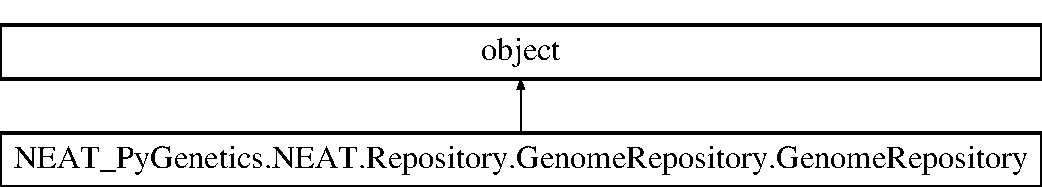
\includegraphics[height=2.000000cm]{classNEAT__PyGenetics_1_1NEAT_1_1Repository_1_1GenomeRepository_1_1GenomeRepository}
\end{center}
\end{figure}
\subsection*{Public Member Functions}
\begin{DoxyCompactItemize}
\item 
def \hyperlink{classNEAT__PyGenetics_1_1NEAT_1_1Repository_1_1GenomeRepository_1_1GenomeRepository_a2d5029444baeba1137a19954fbdc5192}{\+\_\+\+\_\+init\+\_\+\+\_\+}
\item 
def \hyperlink{classNEAT__PyGenetics_1_1NEAT_1_1Repository_1_1GenomeRepository_1_1GenomeRepository_a02f46e4d4d2d09b0ac2b69174f49e129}{get\+\_\+current\+\_\+population} (self)
\begin{DoxyCompactList}\small\item\em \+:return\+: Iterable\mbox{[}Storage\+Genomes\mbox{]} which are alive \end{DoxyCompactList}\item 
def \hyperlink{classNEAT__PyGenetics_1_1NEAT_1_1Repository_1_1GenomeRepository_1_1GenomeRepository_ac55f0529efead778623d6e3eadafa138}{get\+\_\+genome\+\_\+by\+\_\+id}
\item 
def \hyperlink{classNEAT__PyGenetics_1_1NEAT_1_1Repository_1_1GenomeRepository_1_1GenomeRepository_a307127db97bbcb6ef6bbb2000e64d36c}{get\+\_\+genomes\+\_\+in\+\_\+cluster}
\item 
def \hyperlink{classNEAT__PyGenetics_1_1NEAT_1_1Repository_1_1GenomeRepository_1_1GenomeRepository_ac5457262e579905f051b3a0e4f14cbae}{insert\+\_\+genome}
\item 
def \hyperlink{classNEAT__PyGenetics_1_1NEAT_1_1Repository_1_1GenomeRepository_1_1GenomeRepository_ae5b9ba3a9e6586e42cefdd9daf1379b3}{insert\+\_\+genomes}
\item 
def \hyperlink{classNEAT__PyGenetics_1_1NEAT_1_1Repository_1_1GenomeRepository_1_1GenomeRepository_a62c182ec66b0b0f2e444f6bd62f212a2}{update\+\_\+genome}
\item 
def \hyperlink{classNEAT__PyGenetics_1_1NEAT_1_1Repository_1_1GenomeRepository_1_1GenomeRepository_af596e230a4ae914fda99e8f8dfdab8a3}{update\+\_\+genomes}
\item 
def \hyperlink{classNEAT__PyGenetics_1_1NEAT_1_1Repository_1_1GenomeRepository_1_1GenomeRepository_a9a4f5e6dc63ce8a858a79bdb331cc62c}{disable\+\_\+genome}
\item 
def \hyperlink{classNEAT__PyGenetics_1_1NEAT_1_1Repository_1_1GenomeRepository_1_1GenomeRepository_aad8da608f4c1919e72453f1671761b8e}{disable\+\_\+genomes}
\item 
def \hyperlink{classNEAT__PyGenetics_1_1NEAT_1_1Repository_1_1GenomeRepository_1_1GenomeRepository_a89e1f1e4680f135c1eba0f8d13314896}{update\+\_\+genome\+\_\+fitness}
\item 
def \hyperlink{classNEAT__PyGenetics_1_1NEAT_1_1Repository_1_1GenomeRepository_1_1GenomeRepository_a6e90ef99f78be7ecddc26d8b73416116}{update\+\_\+genomes\+\_\+fitness}
\item 
def \hyperlink{classNEAT__PyGenetics_1_1NEAT_1_1Repository_1_1GenomeRepository_1_1GenomeRepository_a1709665aff216c7567cbc079bc5135c8}{update\+\_\+genome\+\_\+cluster}
\end{DoxyCompactItemize}
\subsection*{Static Public Member Functions}
\begin{DoxyCompactItemize}
\item 
def \hyperlink{classNEAT__PyGenetics_1_1NEAT_1_1Repository_1_1GenomeRepository_1_1GenomeRepository_a2ac10279f99269dc45fb9ed047c37fb9}{get\+\_\+new\+\_\+genome} ()
\begin{DoxyCompactList}\small\item\em \+:return\+: Storage\+Genome new Storage\+Genome \end{DoxyCompactList}\end{DoxyCompactItemize}
\subsection*{Static Public Attributes}
\begin{DoxyCompactItemize}
\item 
\hyperlink{classNEAT__PyGenetics_1_1NEAT_1_1Repository_1_1GenomeRepository_1_1GenomeRepository_a23662b9337cfca1f402b206989747f45}{genome}
\item 
\hyperlink{classNEAT__PyGenetics_1_1NEAT_1_1Repository_1_1GenomeRepository_1_1GenomeRepository_a8932d6257b6a5e28ddc6aa822585eef0}{cluster}
\end{DoxyCompactItemize}


\subsection{Constructor \& Destructor Documentation}
\index{N\+E\+A\+T\+\_\+\+Py\+Genetics\+::\+N\+E\+A\+T\+::\+Repository\+::\+Genome\+Repository\+::\+Genome\+Repository@{N\+E\+A\+T\+\_\+\+Py\+Genetics\+::\+N\+E\+A\+T\+::\+Repository\+::\+Genome\+Repository\+::\+Genome\+Repository}!\+\_\+\+\_\+init\+\_\+\+\_\+@{\+\_\+\+\_\+init\+\_\+\+\_\+}}
\index{\+\_\+\+\_\+init\+\_\+\+\_\+@{\+\_\+\+\_\+init\+\_\+\+\_\+}!N\+E\+A\+T\+\_\+\+Py\+Genetics\+::\+N\+E\+A\+T\+::\+Repository\+::\+Genome\+Repository\+::\+Genome\+Repository@{N\+E\+A\+T\+\_\+\+Py\+Genetics\+::\+N\+E\+A\+T\+::\+Repository\+::\+Genome\+Repository\+::\+Genome\+Repository}}
\subsubsection[{\texorpdfstring{\+\_\+\+\_\+init\+\_\+\+\_\+}{__init__}}]{\setlength{\rightskip}{0pt plus 5cm}def N\+E\+A\+T\+\_\+\+Py\+Genetics.\+N\+E\+A\+T.\+Repository.\+Genome\+Repository.\+Genome\+Repository.\+\_\+\+\_\+init\+\_\+\+\_\+ (
\begin{DoxyParamCaption}
\item[{}]{self, }
\item[{}]{database\+\_\+connector}
\end{DoxyParamCaption}
)}\hypertarget{classNEAT__PyGenetics_1_1NEAT_1_1Repository_1_1GenomeRepository_1_1GenomeRepository_a2d5029444baeba1137a19954fbdc5192}{}\label{classNEAT__PyGenetics_1_1NEAT_1_1Repository_1_1GenomeRepository_1_1GenomeRepository_a2d5029444baeba1137a19954fbdc5192}


\subsection{Member Function Documentation}
\index{N\+E\+A\+T\+\_\+\+Py\+Genetics\+::\+N\+E\+A\+T\+::\+Repository\+::\+Genome\+Repository\+::\+Genome\+Repository@{N\+E\+A\+T\+\_\+\+Py\+Genetics\+::\+N\+E\+A\+T\+::\+Repository\+::\+Genome\+Repository\+::\+Genome\+Repository}!disable\+\_\+genome@{disable\+\_\+genome}}
\index{disable\+\_\+genome@{disable\+\_\+genome}!N\+E\+A\+T\+\_\+\+Py\+Genetics\+::\+N\+E\+A\+T\+::\+Repository\+::\+Genome\+Repository\+::\+Genome\+Repository@{N\+E\+A\+T\+\_\+\+Py\+Genetics\+::\+N\+E\+A\+T\+::\+Repository\+::\+Genome\+Repository\+::\+Genome\+Repository}}
\subsubsection[{\texorpdfstring{disable\+\_\+genome}{disable_genome}}]{\setlength{\rightskip}{0pt plus 5cm}def N\+E\+A\+T\+\_\+\+Py\+Genetics.\+N\+E\+A\+T.\+Repository.\+Genome\+Repository.\+Genome\+Repository.\+disable\+\_\+genome (
\begin{DoxyParamCaption}
\item[{}]{self, }
\item[{}]{genome\+\_\+id}
\end{DoxyParamCaption}
)}\hypertarget{classNEAT__PyGenetics_1_1NEAT_1_1Repository_1_1GenomeRepository_1_1GenomeRepository_a9a4f5e6dc63ce8a858a79bdb331cc62c}{}\label{classNEAT__PyGenetics_1_1NEAT_1_1Repository_1_1GenomeRepository_1_1GenomeRepository_a9a4f5e6dc63ce8a858a79bdb331cc62c}
\index{N\+E\+A\+T\+\_\+\+Py\+Genetics\+::\+N\+E\+A\+T\+::\+Repository\+::\+Genome\+Repository\+::\+Genome\+Repository@{N\+E\+A\+T\+\_\+\+Py\+Genetics\+::\+N\+E\+A\+T\+::\+Repository\+::\+Genome\+Repository\+::\+Genome\+Repository}!disable\+\_\+genomes@{disable\+\_\+genomes}}
\index{disable\+\_\+genomes@{disable\+\_\+genomes}!N\+E\+A\+T\+\_\+\+Py\+Genetics\+::\+N\+E\+A\+T\+::\+Repository\+::\+Genome\+Repository\+::\+Genome\+Repository@{N\+E\+A\+T\+\_\+\+Py\+Genetics\+::\+N\+E\+A\+T\+::\+Repository\+::\+Genome\+Repository\+::\+Genome\+Repository}}
\subsubsection[{\texorpdfstring{disable\+\_\+genomes}{disable_genomes}}]{\setlength{\rightskip}{0pt plus 5cm}def N\+E\+A\+T\+\_\+\+Py\+Genetics.\+N\+E\+A\+T.\+Repository.\+Genome\+Repository.\+Genome\+Repository.\+disable\+\_\+genomes (
\begin{DoxyParamCaption}
\item[{}]{self, }
\item[{}]{genomes\+\_\+id}
\end{DoxyParamCaption}
)}\hypertarget{classNEAT__PyGenetics_1_1NEAT_1_1Repository_1_1GenomeRepository_1_1GenomeRepository_aad8da608f4c1919e72453f1671761b8e}{}\label{classNEAT__PyGenetics_1_1NEAT_1_1Repository_1_1GenomeRepository_1_1GenomeRepository_aad8da608f4c1919e72453f1671761b8e}
\index{N\+E\+A\+T\+\_\+\+Py\+Genetics\+::\+N\+E\+A\+T\+::\+Repository\+::\+Genome\+Repository\+::\+Genome\+Repository@{N\+E\+A\+T\+\_\+\+Py\+Genetics\+::\+N\+E\+A\+T\+::\+Repository\+::\+Genome\+Repository\+::\+Genome\+Repository}!get\+\_\+current\+\_\+population@{get\+\_\+current\+\_\+population}}
\index{get\+\_\+current\+\_\+population@{get\+\_\+current\+\_\+population}!N\+E\+A\+T\+\_\+\+Py\+Genetics\+::\+N\+E\+A\+T\+::\+Repository\+::\+Genome\+Repository\+::\+Genome\+Repository@{N\+E\+A\+T\+\_\+\+Py\+Genetics\+::\+N\+E\+A\+T\+::\+Repository\+::\+Genome\+Repository\+::\+Genome\+Repository}}
\subsubsection[{\texorpdfstring{get\+\_\+current\+\_\+population(self)}{get_current_population(self)}}]{\setlength{\rightskip}{0pt plus 5cm}def N\+E\+A\+T\+\_\+\+Py\+Genetics.\+N\+E\+A\+T.\+Repository.\+Genome\+Repository.\+Genome\+Repository.\+get\+\_\+current\+\_\+population (
\begin{DoxyParamCaption}
\item[{}]{self, }
\item[{}]{Iterable, }
\item[{}]{Storage\+Genome}
\end{DoxyParamCaption}
)}\hypertarget{classNEAT__PyGenetics_1_1NEAT_1_1Repository_1_1GenomeRepository_1_1GenomeRepository_a02f46e4d4d2d09b0ac2b69174f49e129}{}\label{classNEAT__PyGenetics_1_1NEAT_1_1Repository_1_1GenomeRepository_1_1GenomeRepository_a02f46e4d4d2d09b0ac2b69174f49e129}


\+:return\+: Iterable\mbox{[}Storage\+Genomes\mbox{]} which are alive 

\index{N\+E\+A\+T\+\_\+\+Py\+Genetics\+::\+N\+E\+A\+T\+::\+Repository\+::\+Genome\+Repository\+::\+Genome\+Repository@{N\+E\+A\+T\+\_\+\+Py\+Genetics\+::\+N\+E\+A\+T\+::\+Repository\+::\+Genome\+Repository\+::\+Genome\+Repository}!get\+\_\+genome\+\_\+by\+\_\+id@{get\+\_\+genome\+\_\+by\+\_\+id}}
\index{get\+\_\+genome\+\_\+by\+\_\+id@{get\+\_\+genome\+\_\+by\+\_\+id}!N\+E\+A\+T\+\_\+\+Py\+Genetics\+::\+N\+E\+A\+T\+::\+Repository\+::\+Genome\+Repository\+::\+Genome\+Repository@{N\+E\+A\+T\+\_\+\+Py\+Genetics\+::\+N\+E\+A\+T\+::\+Repository\+::\+Genome\+Repository\+::\+Genome\+Repository}}
\subsubsection[{\texorpdfstring{get\+\_\+genome\+\_\+by\+\_\+id}{get_genome_by_id}}]{\setlength{\rightskip}{0pt plus 5cm}def N\+E\+A\+T\+\_\+\+Py\+Genetics.\+N\+E\+A\+T.\+Repository.\+Genome\+Repository.\+Genome\+Repository.\+get\+\_\+genome\+\_\+by\+\_\+id (
\begin{DoxyParamCaption}
\item[{}]{self, }
\item[{}]{genome\+\_\+id}
\end{DoxyParamCaption}
)}\hypertarget{classNEAT__PyGenetics_1_1NEAT_1_1Repository_1_1GenomeRepository_1_1GenomeRepository_ac55f0529efead778623d6e3eadafa138}{}\label{classNEAT__PyGenetics_1_1NEAT_1_1Repository_1_1GenomeRepository_1_1GenomeRepository_ac55f0529efead778623d6e3eadafa138}
\index{N\+E\+A\+T\+\_\+\+Py\+Genetics\+::\+N\+E\+A\+T\+::\+Repository\+::\+Genome\+Repository\+::\+Genome\+Repository@{N\+E\+A\+T\+\_\+\+Py\+Genetics\+::\+N\+E\+A\+T\+::\+Repository\+::\+Genome\+Repository\+::\+Genome\+Repository}!get\+\_\+genomes\+\_\+in\+\_\+cluster@{get\+\_\+genomes\+\_\+in\+\_\+cluster}}
\index{get\+\_\+genomes\+\_\+in\+\_\+cluster@{get\+\_\+genomes\+\_\+in\+\_\+cluster}!N\+E\+A\+T\+\_\+\+Py\+Genetics\+::\+N\+E\+A\+T\+::\+Repository\+::\+Genome\+Repository\+::\+Genome\+Repository@{N\+E\+A\+T\+\_\+\+Py\+Genetics\+::\+N\+E\+A\+T\+::\+Repository\+::\+Genome\+Repository\+::\+Genome\+Repository}}
\subsubsection[{\texorpdfstring{get\+\_\+genomes\+\_\+in\+\_\+cluster}{get_genomes_in_cluster}}]{\setlength{\rightskip}{0pt plus 5cm}def N\+E\+A\+T\+\_\+\+Py\+Genetics.\+N\+E\+A\+T.\+Repository.\+Genome\+Repository.\+Genome\+Repository.\+get\+\_\+genomes\+\_\+in\+\_\+cluster (
\begin{DoxyParamCaption}
\item[{}]{self, }
\item[{}]{cluster\+\_\+id}
\end{DoxyParamCaption}
)}\hypertarget{classNEAT__PyGenetics_1_1NEAT_1_1Repository_1_1GenomeRepository_1_1GenomeRepository_a307127db97bbcb6ef6bbb2000e64d36c}{}\label{classNEAT__PyGenetics_1_1NEAT_1_1Repository_1_1GenomeRepository_1_1GenomeRepository_a307127db97bbcb6ef6bbb2000e64d36c}
\index{N\+E\+A\+T\+\_\+\+Py\+Genetics\+::\+N\+E\+A\+T\+::\+Repository\+::\+Genome\+Repository\+::\+Genome\+Repository@{N\+E\+A\+T\+\_\+\+Py\+Genetics\+::\+N\+E\+A\+T\+::\+Repository\+::\+Genome\+Repository\+::\+Genome\+Repository}!get\+\_\+new\+\_\+genome@{get\+\_\+new\+\_\+genome}}
\index{get\+\_\+new\+\_\+genome@{get\+\_\+new\+\_\+genome}!N\+E\+A\+T\+\_\+\+Py\+Genetics\+::\+N\+E\+A\+T\+::\+Repository\+::\+Genome\+Repository\+::\+Genome\+Repository@{N\+E\+A\+T\+\_\+\+Py\+Genetics\+::\+N\+E\+A\+T\+::\+Repository\+::\+Genome\+Repository\+::\+Genome\+Repository}}
\subsubsection[{\texorpdfstring{get\+\_\+new\+\_\+genome()}{get_new_genome()}}]{\setlength{\rightskip}{0pt plus 5cm}def N\+E\+A\+T\+\_\+\+Py\+Genetics.\+N\+E\+A\+T.\+Repository.\+Genome\+Repository.\+Genome\+Repository.\+get\+\_\+new\+\_\+genome (
\begin{DoxyParamCaption}
\item[{}]{Storage\+Genome}
\end{DoxyParamCaption}
)\hspace{0.3cm}{\ttfamily [static]}}\hypertarget{classNEAT__PyGenetics_1_1NEAT_1_1Repository_1_1GenomeRepository_1_1GenomeRepository_a2ac10279f99269dc45fb9ed047c37fb9}{}\label{classNEAT__PyGenetics_1_1NEAT_1_1Repository_1_1GenomeRepository_1_1GenomeRepository_a2ac10279f99269dc45fb9ed047c37fb9}


\+:return\+: Storage\+Genome new Storage\+Genome 

\index{N\+E\+A\+T\+\_\+\+Py\+Genetics\+::\+N\+E\+A\+T\+::\+Repository\+::\+Genome\+Repository\+::\+Genome\+Repository@{N\+E\+A\+T\+\_\+\+Py\+Genetics\+::\+N\+E\+A\+T\+::\+Repository\+::\+Genome\+Repository\+::\+Genome\+Repository}!insert\+\_\+genome@{insert\+\_\+genome}}
\index{insert\+\_\+genome@{insert\+\_\+genome}!N\+E\+A\+T\+\_\+\+Py\+Genetics\+::\+N\+E\+A\+T\+::\+Repository\+::\+Genome\+Repository\+::\+Genome\+Repository@{N\+E\+A\+T\+\_\+\+Py\+Genetics\+::\+N\+E\+A\+T\+::\+Repository\+::\+Genome\+Repository\+::\+Genome\+Repository}}
\subsubsection[{\texorpdfstring{insert\+\_\+genome}{insert_genome}}]{\setlength{\rightskip}{0pt plus 5cm}def N\+E\+A\+T\+\_\+\+Py\+Genetics.\+N\+E\+A\+T.\+Repository.\+Genome\+Repository.\+Genome\+Repository.\+insert\+\_\+genome (
\begin{DoxyParamCaption}
\item[{}]{self, }
\item[{}]{genome}
\end{DoxyParamCaption}
)}\hypertarget{classNEAT__PyGenetics_1_1NEAT_1_1Repository_1_1GenomeRepository_1_1GenomeRepository_ac5457262e579905f051b3a0e4f14cbae}{}\label{classNEAT__PyGenetics_1_1NEAT_1_1Repository_1_1GenomeRepository_1_1GenomeRepository_ac5457262e579905f051b3a0e4f14cbae}
\index{N\+E\+A\+T\+\_\+\+Py\+Genetics\+::\+N\+E\+A\+T\+::\+Repository\+::\+Genome\+Repository\+::\+Genome\+Repository@{N\+E\+A\+T\+\_\+\+Py\+Genetics\+::\+N\+E\+A\+T\+::\+Repository\+::\+Genome\+Repository\+::\+Genome\+Repository}!insert\+\_\+genomes@{insert\+\_\+genomes}}
\index{insert\+\_\+genomes@{insert\+\_\+genomes}!N\+E\+A\+T\+\_\+\+Py\+Genetics\+::\+N\+E\+A\+T\+::\+Repository\+::\+Genome\+Repository\+::\+Genome\+Repository@{N\+E\+A\+T\+\_\+\+Py\+Genetics\+::\+N\+E\+A\+T\+::\+Repository\+::\+Genome\+Repository\+::\+Genome\+Repository}}
\subsubsection[{\texorpdfstring{insert\+\_\+genomes}{insert_genomes}}]{\setlength{\rightskip}{0pt plus 5cm}def N\+E\+A\+T\+\_\+\+Py\+Genetics.\+N\+E\+A\+T.\+Repository.\+Genome\+Repository.\+Genome\+Repository.\+insert\+\_\+genomes (
\begin{DoxyParamCaption}
\item[{}]{self, }
\item[{}]{genomes}
\end{DoxyParamCaption}
)}\hypertarget{classNEAT__PyGenetics_1_1NEAT_1_1Repository_1_1GenomeRepository_1_1GenomeRepository_ae5b9ba3a9e6586e42cefdd9daf1379b3}{}\label{classNEAT__PyGenetics_1_1NEAT_1_1Repository_1_1GenomeRepository_1_1GenomeRepository_ae5b9ba3a9e6586e42cefdd9daf1379b3}
\index{N\+E\+A\+T\+\_\+\+Py\+Genetics\+::\+N\+E\+A\+T\+::\+Repository\+::\+Genome\+Repository\+::\+Genome\+Repository@{N\+E\+A\+T\+\_\+\+Py\+Genetics\+::\+N\+E\+A\+T\+::\+Repository\+::\+Genome\+Repository\+::\+Genome\+Repository}!update\+\_\+genome@{update\+\_\+genome}}
\index{update\+\_\+genome@{update\+\_\+genome}!N\+E\+A\+T\+\_\+\+Py\+Genetics\+::\+N\+E\+A\+T\+::\+Repository\+::\+Genome\+Repository\+::\+Genome\+Repository@{N\+E\+A\+T\+\_\+\+Py\+Genetics\+::\+N\+E\+A\+T\+::\+Repository\+::\+Genome\+Repository\+::\+Genome\+Repository}}
\subsubsection[{\texorpdfstring{update\+\_\+genome}{update_genome}}]{\setlength{\rightskip}{0pt plus 5cm}def N\+E\+A\+T\+\_\+\+Py\+Genetics.\+N\+E\+A\+T.\+Repository.\+Genome\+Repository.\+Genome\+Repository.\+update\+\_\+genome (
\begin{DoxyParamCaption}
\item[{}]{self, }
\item[{}]{genome}
\end{DoxyParamCaption}
)}\hypertarget{classNEAT__PyGenetics_1_1NEAT_1_1Repository_1_1GenomeRepository_1_1GenomeRepository_a62c182ec66b0b0f2e444f6bd62f212a2}{}\label{classNEAT__PyGenetics_1_1NEAT_1_1Repository_1_1GenomeRepository_1_1GenomeRepository_a62c182ec66b0b0f2e444f6bd62f212a2}
\index{N\+E\+A\+T\+\_\+\+Py\+Genetics\+::\+N\+E\+A\+T\+::\+Repository\+::\+Genome\+Repository\+::\+Genome\+Repository@{N\+E\+A\+T\+\_\+\+Py\+Genetics\+::\+N\+E\+A\+T\+::\+Repository\+::\+Genome\+Repository\+::\+Genome\+Repository}!update\+\_\+genome\+\_\+cluster@{update\+\_\+genome\+\_\+cluster}}
\index{update\+\_\+genome\+\_\+cluster@{update\+\_\+genome\+\_\+cluster}!N\+E\+A\+T\+\_\+\+Py\+Genetics\+::\+N\+E\+A\+T\+::\+Repository\+::\+Genome\+Repository\+::\+Genome\+Repository@{N\+E\+A\+T\+\_\+\+Py\+Genetics\+::\+N\+E\+A\+T\+::\+Repository\+::\+Genome\+Repository\+::\+Genome\+Repository}}
\subsubsection[{\texorpdfstring{update\+\_\+genome\+\_\+cluster}{update_genome_cluster}}]{\setlength{\rightskip}{0pt plus 5cm}def N\+E\+A\+T\+\_\+\+Py\+Genetics.\+N\+E\+A\+T.\+Repository.\+Genome\+Repository.\+Genome\+Repository.\+update\+\_\+genome\+\_\+cluster (
\begin{DoxyParamCaption}
\item[{}]{self, }
\item[{}]{genome\+\_\+id}
\end{DoxyParamCaption}
)}\hypertarget{classNEAT__PyGenetics_1_1NEAT_1_1Repository_1_1GenomeRepository_1_1GenomeRepository_a1709665aff216c7567cbc079bc5135c8}{}\label{classNEAT__PyGenetics_1_1NEAT_1_1Repository_1_1GenomeRepository_1_1GenomeRepository_a1709665aff216c7567cbc079bc5135c8}
\index{N\+E\+A\+T\+\_\+\+Py\+Genetics\+::\+N\+E\+A\+T\+::\+Repository\+::\+Genome\+Repository\+::\+Genome\+Repository@{N\+E\+A\+T\+\_\+\+Py\+Genetics\+::\+N\+E\+A\+T\+::\+Repository\+::\+Genome\+Repository\+::\+Genome\+Repository}!update\+\_\+genome\+\_\+fitness@{update\+\_\+genome\+\_\+fitness}}
\index{update\+\_\+genome\+\_\+fitness@{update\+\_\+genome\+\_\+fitness}!N\+E\+A\+T\+\_\+\+Py\+Genetics\+::\+N\+E\+A\+T\+::\+Repository\+::\+Genome\+Repository\+::\+Genome\+Repository@{N\+E\+A\+T\+\_\+\+Py\+Genetics\+::\+N\+E\+A\+T\+::\+Repository\+::\+Genome\+Repository\+::\+Genome\+Repository}}
\subsubsection[{\texorpdfstring{update\+\_\+genome\+\_\+fitness}{update_genome_fitness}}]{\setlength{\rightskip}{0pt plus 5cm}def N\+E\+A\+T\+\_\+\+Py\+Genetics.\+N\+E\+A\+T.\+Repository.\+Genome\+Repository.\+Genome\+Repository.\+update\+\_\+genome\+\_\+fitness (
\begin{DoxyParamCaption}
\item[{}]{self, }
\item[{}]{genome\+\_\+id}
\end{DoxyParamCaption}
)}\hypertarget{classNEAT__PyGenetics_1_1NEAT_1_1Repository_1_1GenomeRepository_1_1GenomeRepository_a89e1f1e4680f135c1eba0f8d13314896}{}\label{classNEAT__PyGenetics_1_1NEAT_1_1Repository_1_1GenomeRepository_1_1GenomeRepository_a89e1f1e4680f135c1eba0f8d13314896}
\index{N\+E\+A\+T\+\_\+\+Py\+Genetics\+::\+N\+E\+A\+T\+::\+Repository\+::\+Genome\+Repository\+::\+Genome\+Repository@{N\+E\+A\+T\+\_\+\+Py\+Genetics\+::\+N\+E\+A\+T\+::\+Repository\+::\+Genome\+Repository\+::\+Genome\+Repository}!update\+\_\+genomes@{update\+\_\+genomes}}
\index{update\+\_\+genomes@{update\+\_\+genomes}!N\+E\+A\+T\+\_\+\+Py\+Genetics\+::\+N\+E\+A\+T\+::\+Repository\+::\+Genome\+Repository\+::\+Genome\+Repository@{N\+E\+A\+T\+\_\+\+Py\+Genetics\+::\+N\+E\+A\+T\+::\+Repository\+::\+Genome\+Repository\+::\+Genome\+Repository}}
\subsubsection[{\texorpdfstring{update\+\_\+genomes}{update_genomes}}]{\setlength{\rightskip}{0pt plus 5cm}def N\+E\+A\+T\+\_\+\+Py\+Genetics.\+N\+E\+A\+T.\+Repository.\+Genome\+Repository.\+Genome\+Repository.\+update\+\_\+genomes (
\begin{DoxyParamCaption}
\item[{}]{self, }
\item[{}]{genomes}
\end{DoxyParamCaption}
)}\hypertarget{classNEAT__PyGenetics_1_1NEAT_1_1Repository_1_1GenomeRepository_1_1GenomeRepository_af596e230a4ae914fda99e8f8dfdab8a3}{}\label{classNEAT__PyGenetics_1_1NEAT_1_1Repository_1_1GenomeRepository_1_1GenomeRepository_af596e230a4ae914fda99e8f8dfdab8a3}
\index{N\+E\+A\+T\+\_\+\+Py\+Genetics\+::\+N\+E\+A\+T\+::\+Repository\+::\+Genome\+Repository\+::\+Genome\+Repository@{N\+E\+A\+T\+\_\+\+Py\+Genetics\+::\+N\+E\+A\+T\+::\+Repository\+::\+Genome\+Repository\+::\+Genome\+Repository}!update\+\_\+genomes\+\_\+fitness@{update\+\_\+genomes\+\_\+fitness}}
\index{update\+\_\+genomes\+\_\+fitness@{update\+\_\+genomes\+\_\+fitness}!N\+E\+A\+T\+\_\+\+Py\+Genetics\+::\+N\+E\+A\+T\+::\+Repository\+::\+Genome\+Repository\+::\+Genome\+Repository@{N\+E\+A\+T\+\_\+\+Py\+Genetics\+::\+N\+E\+A\+T\+::\+Repository\+::\+Genome\+Repository\+::\+Genome\+Repository}}
\subsubsection[{\texorpdfstring{update\+\_\+genomes\+\_\+fitness}{update_genomes_fitness}}]{\setlength{\rightskip}{0pt plus 5cm}def N\+E\+A\+T\+\_\+\+Py\+Genetics.\+N\+E\+A\+T.\+Repository.\+Genome\+Repository.\+Genome\+Repository.\+update\+\_\+genomes\+\_\+fitness (
\begin{DoxyParamCaption}
\item[{}]{self, }
\item[{}]{genome\+\_\+fitness}
\end{DoxyParamCaption}
)}\hypertarget{classNEAT__PyGenetics_1_1NEAT_1_1Repository_1_1GenomeRepository_1_1GenomeRepository_a6e90ef99f78be7ecddc26d8b73416116}{}\label{classNEAT__PyGenetics_1_1NEAT_1_1Repository_1_1GenomeRepository_1_1GenomeRepository_a6e90ef99f78be7ecddc26d8b73416116}


\subsection{Member Data Documentation}
\index{N\+E\+A\+T\+\_\+\+Py\+Genetics\+::\+N\+E\+A\+T\+::\+Repository\+::\+Genome\+Repository\+::\+Genome\+Repository@{N\+E\+A\+T\+\_\+\+Py\+Genetics\+::\+N\+E\+A\+T\+::\+Repository\+::\+Genome\+Repository\+::\+Genome\+Repository}!cluster@{cluster}}
\index{cluster@{cluster}!N\+E\+A\+T\+\_\+\+Py\+Genetics\+::\+N\+E\+A\+T\+::\+Repository\+::\+Genome\+Repository\+::\+Genome\+Repository@{N\+E\+A\+T\+\_\+\+Py\+Genetics\+::\+N\+E\+A\+T\+::\+Repository\+::\+Genome\+Repository\+::\+Genome\+Repository}}
\subsubsection[{\texorpdfstring{cluster}{cluster}}]{\setlength{\rightskip}{0pt plus 5cm}N\+E\+A\+T\+\_\+\+Py\+Genetics.\+N\+E\+A\+T.\+Repository.\+Genome\+Repository.\+Genome\+Repository.\+cluster\hspace{0.3cm}{\ttfamily [static]}}\hypertarget{classNEAT__PyGenetics_1_1NEAT_1_1Repository_1_1GenomeRepository_1_1GenomeRepository_a8932d6257b6a5e28ddc6aa822585eef0}{}\label{classNEAT__PyGenetics_1_1NEAT_1_1Repository_1_1GenomeRepository_1_1GenomeRepository_a8932d6257b6a5e28ddc6aa822585eef0}
\index{N\+E\+A\+T\+\_\+\+Py\+Genetics\+::\+N\+E\+A\+T\+::\+Repository\+::\+Genome\+Repository\+::\+Genome\+Repository@{N\+E\+A\+T\+\_\+\+Py\+Genetics\+::\+N\+E\+A\+T\+::\+Repository\+::\+Genome\+Repository\+::\+Genome\+Repository}!genome@{genome}}
\index{genome@{genome}!N\+E\+A\+T\+\_\+\+Py\+Genetics\+::\+N\+E\+A\+T\+::\+Repository\+::\+Genome\+Repository\+::\+Genome\+Repository@{N\+E\+A\+T\+\_\+\+Py\+Genetics\+::\+N\+E\+A\+T\+::\+Repository\+::\+Genome\+Repository\+::\+Genome\+Repository}}
\subsubsection[{\texorpdfstring{genome}{genome}}]{\setlength{\rightskip}{0pt plus 5cm}N\+E\+A\+T\+\_\+\+Py\+Genetics.\+N\+E\+A\+T.\+Repository.\+Genome\+Repository.\+Genome\+Repository.\+genome\hspace{0.3cm}{\ttfamily [static]}}\hypertarget{classNEAT__PyGenetics_1_1NEAT_1_1Repository_1_1GenomeRepository_1_1GenomeRepository_a23662b9337cfca1f402b206989747f45}{}\label{classNEAT__PyGenetics_1_1NEAT_1_1Repository_1_1GenomeRepository_1_1GenomeRepository_a23662b9337cfca1f402b206989747f45}


The documentation for this class was generated from the following file\+:\begin{DoxyCompactItemize}
\item 
N\+E\+A\+T/\+Repository/\hyperlink{GenomeRepository_8py}{Genome\+Repository.\+py}\end{DoxyCompactItemize}

\hypertarget{classNEAT__PyGenetics_1_1NEAT_1_1Analyst_1_1GenomeSelector_1_1GenomeSelector}{}\section{N\+E\+A\+T\+\_\+\+Py\+Genetics.\+N\+E\+A\+T.\+Analyst.\+Genome\+Selector.\+Genome\+Selector Class Reference}
\label{classNEAT__PyGenetics_1_1NEAT_1_1Analyst_1_1GenomeSelector_1_1GenomeSelector}\index{N\+E\+A\+T\+\_\+\+Py\+Genetics.\+N\+E\+A\+T.\+Analyst.\+Genome\+Selector.\+Genome\+Selector@{N\+E\+A\+T\+\_\+\+Py\+Genetics.\+N\+E\+A\+T.\+Analyst.\+Genome\+Selector.\+Genome\+Selector}}
Inheritance diagram for N\+E\+A\+T\+\_\+\+Py\+Genetics.\+N\+E\+A\+T.\+Analyst.\+Genome\+Selector.\+Genome\+Selector\+:\begin{figure}[H]
\begin{center}
\leavevmode
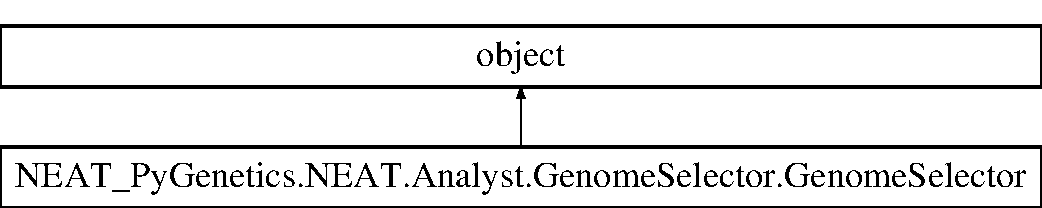
\includegraphics[height=2.000000cm]{classNEAT__PyGenetics_1_1NEAT_1_1Analyst_1_1GenomeSelector_1_1GenomeSelector}
\end{center}
\end{figure}
\subsection*{Public Member Functions}
\begin{DoxyCompactItemize}
\item 
def \hyperlink{classNEAT__PyGenetics_1_1NEAT_1_1Analyst_1_1GenomeSelector_1_1GenomeSelector_a92cb92afdabf4246963cf8214c9baa76}{\+\_\+\+\_\+init\+\_\+\+\_\+}
\begin{DoxyCompactList}\small\item\em \+:param genome\+\_\+repository\+: Genome\+Repository to select \+:param cluster\+\_\+repository\+: Cluster\+Repository to select \+:param selection\+\_\+parameters\+: saved in selection.\+conf \+:return\+: \end{DoxyCompactList}\item 
def \hyperlink{classNEAT__PyGenetics_1_1NEAT_1_1Analyst_1_1GenomeSelector_1_1GenomeSelector_aae7092166920c907176530a60deda37d}{get\+\_\+genomes\+\_\+in\+\_\+cluster}
\begin{DoxyCompactList}\small\item\em Selects and Area of genomes in \hyperlink{namespaceNEAT__PyGenetics_1_1NEAT_1_1Analyst_1_1Cluster}{Cluster} given by input offspring. \end{DoxyCompactList}\item 
def \hyperlink{classNEAT__PyGenetics_1_1NEAT_1_1Analyst_1_1GenomeSelector_1_1GenomeSelector_a2fb8600454d9d808158dbe3ace6b4952}{get\+\_\+cluster\+\_\+area\+\_\+sorted\+\_\+by\+\_\+fitness}
\begin{DoxyCompactList}\small\item\em \+:param begin\+: float percentage starting area (0 is starting by weakest) \+:param ending\+: float ending area (1 is starting by fitt est) \+:return\+: List\mbox{[}\hyperlink{namespaceNEAT__PyGenetics_1_1NEAT_1_1Analyst_1_1Cluster}{Cluster}\mbox{]} sorted by fitness \end{DoxyCompactList}\item 
def \hyperlink{classNEAT__PyGenetics_1_1NEAT_1_1Analyst_1_1GenomeSelector_1_1GenomeSelector_a938d385b8d73983a5e9abf75a80f03f5}{select\+\_\+genomes\+\_\+for\+\_\+breeding}
\begin{DoxyCompactList}\small\item\em Selects genomes for breeding currently best two from all Clusters \+:type breeding\+\_\+percentage\+: float \+:return\+: tuple(\+Storage) \end{DoxyCompactList}\item 
def \hyperlink{classNEAT__PyGenetics_1_1NEAT_1_1Analyst_1_1GenomeSelector_1_1GenomeSelector_af335a5342b0a1695c52d61274c83b0bf}{select\+\_\+genomes\+\_\+for\+\_\+mutation}
\begin{DoxyCompactList}\small\item\em Selects genome for mutation currently the best from all Clusters \+:param mutation\+\_\+percentage\+: float \+:return\+: Storage\+Genome the most fit. \end{DoxyCompactList}\item 
def \hyperlink{classNEAT__PyGenetics_1_1NEAT_1_1Analyst_1_1GenomeSelector_1_1GenomeSelector_a9e1d64bae210147a47049f1c8c389bfc}{select\+\_\+clusters\+\_\+for\+\_\+combination} (self)
\begin{DoxyCompactList}\small\item\em \+:return\+: Tuple\mbox{[}\hyperlink{namespaceNEAT__PyGenetics_1_1NEAT_1_1Analyst_1_1Cluster}{Cluster}\mbox{]} cluster chosen for combination \end{DoxyCompactList}\item 
def \hyperlink{classNEAT__PyGenetics_1_1NEAT_1_1Analyst_1_1GenomeSelector_1_1GenomeSelector_a08b5d1264a5dadc1ec98affabf1ab76d}{select\+\_\+cluster\+\_\+combinations}
\begin{DoxyCompactList}\small\item\em \+:param cluster1\+: \hyperlink{namespaceNEAT__PyGenetics_1_1NEAT_1_1Analyst_1_1Cluster}{Cluster} to choose 1 \+:param cluster2\+: \hyperlink{namespaceNEAT__PyGenetics_1_1NEAT_1_1Analyst_1_1Cluster}{Cluster} to choose 2 \+:param genome\+\_\+count\+: int number of seats which should be filled \+:return\+: List\mbox{[}Tuple\mbox{[}Storage\+Genome\mbox{]}\mbox{]} combination from given cluster \end{DoxyCompactList}\item 
def \hyperlink{classNEAT__PyGenetics_1_1NEAT_1_1Analyst_1_1GenomeSelector_1_1GenomeSelector_a1016a10b5301bd2a1fd770dceda6644b}{select\+\_\+clusters\+\_\+for\+\_\+discarding} (self)
\begin{DoxyCompactList}\small\item\em select x percentage (given by selection.\+conf \char`\"{}discarding\+\_\+by\+\_\+cluster\+\_\+fitness\char`\"{}) of \hyperlink{namespaceNEAT__PyGenetics_1_1NEAT_1_1Analyst_1_1Cluster}{Cluster} sorted ascending by fitness \+:return\+: List of \hyperlink{namespaceNEAT__PyGenetics_1_1NEAT_1_1Analyst_1_1Cluster}{Cluster} wanted to be discarded \end{DoxyCompactList}\item 
def \hyperlink{classNEAT__PyGenetics_1_1NEAT_1_1Analyst_1_1GenomeSelector_1_1GenomeSelector_af7cd898b9a5bbc1e2e407256a385f865}{select\+\_\+genomes\+\_\+for\+\_\+discarding} (self)
\begin{DoxyCompactList}\small\item\em select \char`\"{}discarding\+\_\+by\+\_\+genome\+\_\+fitness\char`\"{} percentage (in every \hyperlink{namespaceNEAT__PyGenetics_1_1NEAT_1_1Analyst_1_1Cluster}{Cluster}) of genomes sorted ascending by fitness \+:return\+: List of Genomes wanted to be discarded \end{DoxyCompactList}\end{DoxyCompactItemize}
\subsection*{Static Public Attributes}
\begin{DoxyCompactItemize}
\item 
\hyperlink{classNEAT__PyGenetics_1_1NEAT_1_1Analyst_1_1GenomeSelector_1_1GenomeSelector_aabb39abd6a1fcfa61f9b8eb4662e00db}{genome\+\_\+repository}
\item 
\hyperlink{classNEAT__PyGenetics_1_1NEAT_1_1Analyst_1_1GenomeSelector_1_1GenomeSelector_ad3561e93fc8fdd2c51ffec388ddc4c7e}{cluster\+\_\+repository}
\item 
\hyperlink{classNEAT__PyGenetics_1_1NEAT_1_1Analyst_1_1GenomeSelector_1_1GenomeSelector_af6ab170d7eef08b15d79eabb074ade5e}{selection\+\_\+parameters}
\item 
\hyperlink{classNEAT__PyGenetics_1_1NEAT_1_1Analyst_1_1GenomeSelector_1_1GenomeSelector_affce7cea247dd2a869d83fbcc67f9f78}{genomes}
\item 
\hyperlink{classNEAT__PyGenetics_1_1NEAT_1_1Analyst_1_1GenomeSelector_1_1GenomeSelector_a65680f48e6b7e8f218f8536420a665db}{clusters}
\item 
\hyperlink{classNEAT__PyGenetics_1_1NEAT_1_1Analyst_1_1GenomeSelector_1_1GenomeSelector_a59881db1a9d315dd4019aad7d52eeeb2}{key}
\item 
\hyperlink{classNEAT__PyGenetics_1_1NEAT_1_1Analyst_1_1GenomeSelector_1_1GenomeSelector_a41d6d1538df7134f2f31519ff49f6c58}{start}
\item 
\hyperlink{classNEAT__PyGenetics_1_1NEAT_1_1Analyst_1_1GenomeSelector_1_1GenomeSelector_a9531d1391e7501950602af5dd854a43a}{end}
\item 
\hyperlink{classNEAT__PyGenetics_1_1NEAT_1_1Analyst_1_1GenomeSelector_1_1GenomeSelector_af361031b936449d59bedda05b9363d13}{result}
\item 
\hyperlink{classNEAT__PyGenetics_1_1NEAT_1_1Analyst_1_1GenomeSelector_1_1GenomeSelector_afa3ff139e2ad867f5746aee243fd9aa1}{genome\+\_\+one}
\item 
\hyperlink{classNEAT__PyGenetics_1_1NEAT_1_1Analyst_1_1GenomeSelector_1_1GenomeSelector_a8ea3993f52a51fe0d93b331eb2b78a8d}{genome\+\_\+two}
\item 
\hyperlink{classNEAT__PyGenetics_1_1NEAT_1_1Analyst_1_1GenomeSelector_1_1GenomeSelector_a22cb93426797917839ba925a79e51a36}{seats\+\_\+to\+\_\+mutation}
\item 
\hyperlink{classNEAT__PyGenetics_1_1NEAT_1_1Analyst_1_1GenomeSelector_1_1GenomeSelector_af8c8af7836b5ae5b52f6688c1266bb06}{step}
\item 
\hyperlink{classNEAT__PyGenetics_1_1NEAT_1_1Analyst_1_1GenomeSelector_1_1GenomeSelector_a2b86adfa98c72c3ce406e95fce29a9ad}{genomes1}
\item 
\hyperlink{classNEAT__PyGenetics_1_1NEAT_1_1Analyst_1_1GenomeSelector_1_1GenomeSelector_aff1676f8a3e91f03ef133d445fd111b8}{genomes2}
\item 
\hyperlink{classNEAT__PyGenetics_1_1NEAT_1_1Analyst_1_1GenomeSelector_1_1GenomeSelector_a66bc085d9c0e2b4ce121fd3c4d4ec226}{g1}
\item 
\hyperlink{classNEAT__PyGenetics_1_1NEAT_1_1Analyst_1_1GenomeSelector_1_1GenomeSelector_a335eeb80af660ac6ef6d5a8ca81fb95c}{g2}
\end{DoxyCompactItemize}


\subsection{Constructor \& Destructor Documentation}
\index{N\+E\+A\+T\+\_\+\+Py\+Genetics\+::\+N\+E\+A\+T\+::\+Analyst\+::\+Genome\+Selector\+::\+Genome\+Selector@{N\+E\+A\+T\+\_\+\+Py\+Genetics\+::\+N\+E\+A\+T\+::\+Analyst\+::\+Genome\+Selector\+::\+Genome\+Selector}!\+\_\+\+\_\+init\+\_\+\+\_\+@{\+\_\+\+\_\+init\+\_\+\+\_\+}}
\index{\+\_\+\+\_\+init\+\_\+\+\_\+@{\+\_\+\+\_\+init\+\_\+\+\_\+}!N\+E\+A\+T\+\_\+\+Py\+Genetics\+::\+N\+E\+A\+T\+::\+Analyst\+::\+Genome\+Selector\+::\+Genome\+Selector@{N\+E\+A\+T\+\_\+\+Py\+Genetics\+::\+N\+E\+A\+T\+::\+Analyst\+::\+Genome\+Selector\+::\+Genome\+Selector}}
\subsubsection[{\texorpdfstring{\+\_\+\+\_\+init\+\_\+\+\_\+}{__init__}}]{\setlength{\rightskip}{0pt plus 5cm}def N\+E\+A\+T\+\_\+\+Py\+Genetics.\+N\+E\+A\+T.\+Analyst.\+Genome\+Selector.\+Genome\+Selector.\+\_\+\+\_\+init\+\_\+\+\_\+ (
\begin{DoxyParamCaption}
\item[{}]{self, }
\item[{}]{genome\+\_\+repository}
\end{DoxyParamCaption}
)}\hypertarget{classNEAT__PyGenetics_1_1NEAT_1_1Analyst_1_1GenomeSelector_1_1GenomeSelector_a92cb92afdabf4246963cf8214c9baa76}{}\label{classNEAT__PyGenetics_1_1NEAT_1_1Analyst_1_1GenomeSelector_1_1GenomeSelector_a92cb92afdabf4246963cf8214c9baa76}


\+:param genome\+\_\+repository\+: Genome\+Repository to select \+:param cluster\+\_\+repository\+: Cluster\+Repository to select \+:param selection\+\_\+parameters\+: saved in selection.\+conf \+:return\+: 



\subsection{Member Function Documentation}
\index{N\+E\+A\+T\+\_\+\+Py\+Genetics\+::\+N\+E\+A\+T\+::\+Analyst\+::\+Genome\+Selector\+::\+Genome\+Selector@{N\+E\+A\+T\+\_\+\+Py\+Genetics\+::\+N\+E\+A\+T\+::\+Analyst\+::\+Genome\+Selector\+::\+Genome\+Selector}!get\+\_\+cluster\+\_\+area\+\_\+sorted\+\_\+by\+\_\+fitness@{get\+\_\+cluster\+\_\+area\+\_\+sorted\+\_\+by\+\_\+fitness}}
\index{get\+\_\+cluster\+\_\+area\+\_\+sorted\+\_\+by\+\_\+fitness@{get\+\_\+cluster\+\_\+area\+\_\+sorted\+\_\+by\+\_\+fitness}!N\+E\+A\+T\+\_\+\+Py\+Genetics\+::\+N\+E\+A\+T\+::\+Analyst\+::\+Genome\+Selector\+::\+Genome\+Selector@{N\+E\+A\+T\+\_\+\+Py\+Genetics\+::\+N\+E\+A\+T\+::\+Analyst\+::\+Genome\+Selector\+::\+Genome\+Selector}}
\subsubsection[{\texorpdfstring{get\+\_\+cluster\+\_\+area\+\_\+sorted\+\_\+by\+\_\+fitness}{get_cluster_area_sorted_by_fitness}}]{\setlength{\rightskip}{0pt plus 5cm}def N\+E\+A\+T\+\_\+\+Py\+Genetics.\+N\+E\+A\+T.\+Analyst.\+Genome\+Selector.\+Genome\+Selector.\+get\+\_\+cluster\+\_\+area\+\_\+sorted\+\_\+by\+\_\+fitness (
\begin{DoxyParamCaption}
\item[{}]{self, }
\item[{}]{begin}
\end{DoxyParamCaption}
)}\hypertarget{classNEAT__PyGenetics_1_1NEAT_1_1Analyst_1_1GenomeSelector_1_1GenomeSelector_a2fb8600454d9d808158dbe3ace6b4952}{}\label{classNEAT__PyGenetics_1_1NEAT_1_1Analyst_1_1GenomeSelector_1_1GenomeSelector_a2fb8600454d9d808158dbe3ace6b4952}


\+:param begin\+: float percentage starting area (0 is starting by weakest) \+:param ending\+: float ending area (1 is starting by fitt est) \+:return\+: List\mbox{[}\hyperlink{namespaceNEAT__PyGenetics_1_1NEAT_1_1Analyst_1_1Cluster}{Cluster}\mbox{]} sorted by fitness 

\index{N\+E\+A\+T\+\_\+\+Py\+Genetics\+::\+N\+E\+A\+T\+::\+Analyst\+::\+Genome\+Selector\+::\+Genome\+Selector@{N\+E\+A\+T\+\_\+\+Py\+Genetics\+::\+N\+E\+A\+T\+::\+Analyst\+::\+Genome\+Selector\+::\+Genome\+Selector}!get\+\_\+genomes\+\_\+in\+\_\+cluster@{get\+\_\+genomes\+\_\+in\+\_\+cluster}}
\index{get\+\_\+genomes\+\_\+in\+\_\+cluster@{get\+\_\+genomes\+\_\+in\+\_\+cluster}!N\+E\+A\+T\+\_\+\+Py\+Genetics\+::\+N\+E\+A\+T\+::\+Analyst\+::\+Genome\+Selector\+::\+Genome\+Selector@{N\+E\+A\+T\+\_\+\+Py\+Genetics\+::\+N\+E\+A\+T\+::\+Analyst\+::\+Genome\+Selector\+::\+Genome\+Selector}}
\subsubsection[{\texorpdfstring{get\+\_\+genomes\+\_\+in\+\_\+cluster}{get_genomes_in_cluster}}]{\setlength{\rightskip}{0pt plus 5cm}def N\+E\+A\+T\+\_\+\+Py\+Genetics.\+N\+E\+A\+T.\+Analyst.\+Genome\+Selector.\+Genome\+Selector.\+get\+\_\+genomes\+\_\+in\+\_\+cluster (
\begin{DoxyParamCaption}
\item[{}]{self, }
\item[{}]{cluster\+\_\+id}
\end{DoxyParamCaption}
)}\hypertarget{classNEAT__PyGenetics_1_1NEAT_1_1Analyst_1_1GenomeSelector_1_1GenomeSelector_aae7092166920c907176530a60deda37d}{}\label{classNEAT__PyGenetics_1_1NEAT_1_1Analyst_1_1GenomeSelector_1_1GenomeSelector_aae7092166920c907176530a60deda37d}


Selects and Area of genomes in \hyperlink{namespaceNEAT__PyGenetics_1_1NEAT_1_1Analyst_1_1Cluster}{Cluster} given by input offspring. 

\+:param cluster\+\_\+id\+: Object\+Id to load Genomes \+:return\+: \mbox{[}Storage\+Genome\mbox{]} \index{N\+E\+A\+T\+\_\+\+Py\+Genetics\+::\+N\+E\+A\+T\+::\+Analyst\+::\+Genome\+Selector\+::\+Genome\+Selector@{N\+E\+A\+T\+\_\+\+Py\+Genetics\+::\+N\+E\+A\+T\+::\+Analyst\+::\+Genome\+Selector\+::\+Genome\+Selector}!select\+\_\+cluster\+\_\+combinations@{select\+\_\+cluster\+\_\+combinations}}
\index{select\+\_\+cluster\+\_\+combinations@{select\+\_\+cluster\+\_\+combinations}!N\+E\+A\+T\+\_\+\+Py\+Genetics\+::\+N\+E\+A\+T\+::\+Analyst\+::\+Genome\+Selector\+::\+Genome\+Selector@{N\+E\+A\+T\+\_\+\+Py\+Genetics\+::\+N\+E\+A\+T\+::\+Analyst\+::\+Genome\+Selector\+::\+Genome\+Selector}}
\subsubsection[{\texorpdfstring{select\+\_\+cluster\+\_\+combinations}{select_cluster_combinations}}]{\setlength{\rightskip}{0pt plus 5cm}def N\+E\+A\+T\+\_\+\+Py\+Genetics.\+N\+E\+A\+T.\+Analyst.\+Genome\+Selector.\+Genome\+Selector.\+select\+\_\+cluster\+\_\+combinations (
\begin{DoxyParamCaption}
\item[{}]{self, }
\item[{}]{cluster1}
\end{DoxyParamCaption}
)}\hypertarget{classNEAT__PyGenetics_1_1NEAT_1_1Analyst_1_1GenomeSelector_1_1GenomeSelector_a08b5d1264a5dadc1ec98affabf1ab76d}{}\label{classNEAT__PyGenetics_1_1NEAT_1_1Analyst_1_1GenomeSelector_1_1GenomeSelector_a08b5d1264a5dadc1ec98affabf1ab76d}


\+:param cluster1\+: \hyperlink{namespaceNEAT__PyGenetics_1_1NEAT_1_1Analyst_1_1Cluster}{Cluster} to choose 1 \+:param cluster2\+: \hyperlink{namespaceNEAT__PyGenetics_1_1NEAT_1_1Analyst_1_1Cluster}{Cluster} to choose 2 \+:param genome\+\_\+count\+: int number of seats which should be filled \+:return\+: List\mbox{[}Tuple\mbox{[}Storage\+Genome\mbox{]}\mbox{]} combination from given cluster 

\index{N\+E\+A\+T\+\_\+\+Py\+Genetics\+::\+N\+E\+A\+T\+::\+Analyst\+::\+Genome\+Selector\+::\+Genome\+Selector@{N\+E\+A\+T\+\_\+\+Py\+Genetics\+::\+N\+E\+A\+T\+::\+Analyst\+::\+Genome\+Selector\+::\+Genome\+Selector}!select\+\_\+clusters\+\_\+for\+\_\+combination@{select\+\_\+clusters\+\_\+for\+\_\+combination}}
\index{select\+\_\+clusters\+\_\+for\+\_\+combination@{select\+\_\+clusters\+\_\+for\+\_\+combination}!N\+E\+A\+T\+\_\+\+Py\+Genetics\+::\+N\+E\+A\+T\+::\+Analyst\+::\+Genome\+Selector\+::\+Genome\+Selector@{N\+E\+A\+T\+\_\+\+Py\+Genetics\+::\+N\+E\+A\+T\+::\+Analyst\+::\+Genome\+Selector\+::\+Genome\+Selector}}
\subsubsection[{\texorpdfstring{select\+\_\+clusters\+\_\+for\+\_\+combination(self)}{select_clusters_for_combination(self)}}]{\setlength{\rightskip}{0pt plus 5cm}def N\+E\+A\+T\+\_\+\+Py\+Genetics.\+N\+E\+A\+T.\+Analyst.\+Genome\+Selector.\+Genome\+Selector.\+select\+\_\+clusters\+\_\+for\+\_\+combination (
\begin{DoxyParamCaption}
\item[{}]{self, }
\item[{}]{Tuple, }
\item[{}]{Cluster, }
\item[{}]{Cluster}
\end{DoxyParamCaption}
)}\hypertarget{classNEAT__PyGenetics_1_1NEAT_1_1Analyst_1_1GenomeSelector_1_1GenomeSelector_a9e1d64bae210147a47049f1c8c389bfc}{}\label{classNEAT__PyGenetics_1_1NEAT_1_1Analyst_1_1GenomeSelector_1_1GenomeSelector_a9e1d64bae210147a47049f1c8c389bfc}


\+:return\+: Tuple\mbox{[}\hyperlink{namespaceNEAT__PyGenetics_1_1NEAT_1_1Analyst_1_1Cluster}{Cluster}\mbox{]} cluster chosen for combination 

\index{N\+E\+A\+T\+\_\+\+Py\+Genetics\+::\+N\+E\+A\+T\+::\+Analyst\+::\+Genome\+Selector\+::\+Genome\+Selector@{N\+E\+A\+T\+\_\+\+Py\+Genetics\+::\+N\+E\+A\+T\+::\+Analyst\+::\+Genome\+Selector\+::\+Genome\+Selector}!select\+\_\+clusters\+\_\+for\+\_\+discarding@{select\+\_\+clusters\+\_\+for\+\_\+discarding}}
\index{select\+\_\+clusters\+\_\+for\+\_\+discarding@{select\+\_\+clusters\+\_\+for\+\_\+discarding}!N\+E\+A\+T\+\_\+\+Py\+Genetics\+::\+N\+E\+A\+T\+::\+Analyst\+::\+Genome\+Selector\+::\+Genome\+Selector@{N\+E\+A\+T\+\_\+\+Py\+Genetics\+::\+N\+E\+A\+T\+::\+Analyst\+::\+Genome\+Selector\+::\+Genome\+Selector}}
\subsubsection[{\texorpdfstring{select\+\_\+clusters\+\_\+for\+\_\+discarding(self)}{select_clusters_for_discarding(self)}}]{\setlength{\rightskip}{0pt plus 5cm}def N\+E\+A\+T\+\_\+\+Py\+Genetics.\+N\+E\+A\+T.\+Analyst.\+Genome\+Selector.\+Genome\+Selector.\+select\+\_\+clusters\+\_\+for\+\_\+discarding (
\begin{DoxyParamCaption}
\item[{}]{self, }
\item[{}]{List, }
\item[{}]{Cluster}
\end{DoxyParamCaption}
)}\hypertarget{classNEAT__PyGenetics_1_1NEAT_1_1Analyst_1_1GenomeSelector_1_1GenomeSelector_a1016a10b5301bd2a1fd770dceda6644b}{}\label{classNEAT__PyGenetics_1_1NEAT_1_1Analyst_1_1GenomeSelector_1_1GenomeSelector_a1016a10b5301bd2a1fd770dceda6644b}


select x percentage (given by selection.\+conf \char`\"{}discarding\+\_\+by\+\_\+cluster\+\_\+fitness\char`\"{}) of \hyperlink{namespaceNEAT__PyGenetics_1_1NEAT_1_1Analyst_1_1Cluster}{Cluster} sorted ascending by fitness \+:return\+: List of \hyperlink{namespaceNEAT__PyGenetics_1_1NEAT_1_1Analyst_1_1Cluster}{Cluster} wanted to be discarded 

\index{N\+E\+A\+T\+\_\+\+Py\+Genetics\+::\+N\+E\+A\+T\+::\+Analyst\+::\+Genome\+Selector\+::\+Genome\+Selector@{N\+E\+A\+T\+\_\+\+Py\+Genetics\+::\+N\+E\+A\+T\+::\+Analyst\+::\+Genome\+Selector\+::\+Genome\+Selector}!select\+\_\+genomes\+\_\+for\+\_\+breeding@{select\+\_\+genomes\+\_\+for\+\_\+breeding}}
\index{select\+\_\+genomes\+\_\+for\+\_\+breeding@{select\+\_\+genomes\+\_\+for\+\_\+breeding}!N\+E\+A\+T\+\_\+\+Py\+Genetics\+::\+N\+E\+A\+T\+::\+Analyst\+::\+Genome\+Selector\+::\+Genome\+Selector@{N\+E\+A\+T\+\_\+\+Py\+Genetics\+::\+N\+E\+A\+T\+::\+Analyst\+::\+Genome\+Selector\+::\+Genome\+Selector}}
\subsubsection[{\texorpdfstring{select\+\_\+genomes\+\_\+for\+\_\+breeding}{select_genomes_for_breeding}}]{\setlength{\rightskip}{0pt plus 5cm}def N\+E\+A\+T\+\_\+\+Py\+Genetics.\+N\+E\+A\+T.\+Analyst.\+Genome\+Selector.\+Genome\+Selector.\+select\+\_\+genomes\+\_\+for\+\_\+breeding (
\begin{DoxyParamCaption}
\item[{}]{self, }
\item[{}]{breeding\+\_\+percentage}
\end{DoxyParamCaption}
)}\hypertarget{classNEAT__PyGenetics_1_1NEAT_1_1Analyst_1_1GenomeSelector_1_1GenomeSelector_a938d385b8d73983a5e9abf75a80f03f5}{}\label{classNEAT__PyGenetics_1_1NEAT_1_1Analyst_1_1GenomeSelector_1_1GenomeSelector_a938d385b8d73983a5e9abf75a80f03f5}


Selects genomes for breeding currently best two from all Clusters \+:type breeding\+\_\+percentage\+: float \+:return\+: tuple(\+Storage) 

\index{N\+E\+A\+T\+\_\+\+Py\+Genetics\+::\+N\+E\+A\+T\+::\+Analyst\+::\+Genome\+Selector\+::\+Genome\+Selector@{N\+E\+A\+T\+\_\+\+Py\+Genetics\+::\+N\+E\+A\+T\+::\+Analyst\+::\+Genome\+Selector\+::\+Genome\+Selector}!select\+\_\+genomes\+\_\+for\+\_\+discarding@{select\+\_\+genomes\+\_\+for\+\_\+discarding}}
\index{select\+\_\+genomes\+\_\+for\+\_\+discarding@{select\+\_\+genomes\+\_\+for\+\_\+discarding}!N\+E\+A\+T\+\_\+\+Py\+Genetics\+::\+N\+E\+A\+T\+::\+Analyst\+::\+Genome\+Selector\+::\+Genome\+Selector@{N\+E\+A\+T\+\_\+\+Py\+Genetics\+::\+N\+E\+A\+T\+::\+Analyst\+::\+Genome\+Selector\+::\+Genome\+Selector}}
\subsubsection[{\texorpdfstring{select\+\_\+genomes\+\_\+for\+\_\+discarding(self)}{select_genomes_for_discarding(self)}}]{\setlength{\rightskip}{0pt plus 5cm}def N\+E\+A\+T\+\_\+\+Py\+Genetics.\+N\+E\+A\+T.\+Analyst.\+Genome\+Selector.\+Genome\+Selector.\+select\+\_\+genomes\+\_\+for\+\_\+discarding (
\begin{DoxyParamCaption}
\item[{}]{self, }
\item[{}]{List, }
\item[{}]{Storage\+Genome}
\end{DoxyParamCaption}
)}\hypertarget{classNEAT__PyGenetics_1_1NEAT_1_1Analyst_1_1GenomeSelector_1_1GenomeSelector_af7cd898b9a5bbc1e2e407256a385f865}{}\label{classNEAT__PyGenetics_1_1NEAT_1_1Analyst_1_1GenomeSelector_1_1GenomeSelector_af7cd898b9a5bbc1e2e407256a385f865}


select \char`\"{}discarding\+\_\+by\+\_\+genome\+\_\+fitness\char`\"{} percentage (in every \hyperlink{namespaceNEAT__PyGenetics_1_1NEAT_1_1Analyst_1_1Cluster}{Cluster}) of genomes sorted ascending by fitness \+:return\+: List of Genomes wanted to be discarded 

\index{N\+E\+A\+T\+\_\+\+Py\+Genetics\+::\+N\+E\+A\+T\+::\+Analyst\+::\+Genome\+Selector\+::\+Genome\+Selector@{N\+E\+A\+T\+\_\+\+Py\+Genetics\+::\+N\+E\+A\+T\+::\+Analyst\+::\+Genome\+Selector\+::\+Genome\+Selector}!select\+\_\+genomes\+\_\+for\+\_\+mutation@{select\+\_\+genomes\+\_\+for\+\_\+mutation}}
\index{select\+\_\+genomes\+\_\+for\+\_\+mutation@{select\+\_\+genomes\+\_\+for\+\_\+mutation}!N\+E\+A\+T\+\_\+\+Py\+Genetics\+::\+N\+E\+A\+T\+::\+Analyst\+::\+Genome\+Selector\+::\+Genome\+Selector@{N\+E\+A\+T\+\_\+\+Py\+Genetics\+::\+N\+E\+A\+T\+::\+Analyst\+::\+Genome\+Selector\+::\+Genome\+Selector}}
\subsubsection[{\texorpdfstring{select\+\_\+genomes\+\_\+for\+\_\+mutation}{select_genomes_for_mutation}}]{\setlength{\rightskip}{0pt plus 5cm}def N\+E\+A\+T\+\_\+\+Py\+Genetics.\+N\+E\+A\+T.\+Analyst.\+Genome\+Selector.\+Genome\+Selector.\+select\+\_\+genomes\+\_\+for\+\_\+mutation (
\begin{DoxyParamCaption}
\item[{}]{self, }
\item[{}]{mutation\+\_\+percentage}
\end{DoxyParamCaption}
)}\hypertarget{classNEAT__PyGenetics_1_1NEAT_1_1Analyst_1_1GenomeSelector_1_1GenomeSelector_af335a5342b0a1695c52d61274c83b0bf}{}\label{classNEAT__PyGenetics_1_1NEAT_1_1Analyst_1_1GenomeSelector_1_1GenomeSelector_af335a5342b0a1695c52d61274c83b0bf}


Selects genome for mutation currently the best from all Clusters \+:param mutation\+\_\+percentage\+: float \+:return\+: Storage\+Genome the most fit. 



\subsection{Member Data Documentation}
\index{N\+E\+A\+T\+\_\+\+Py\+Genetics\+::\+N\+E\+A\+T\+::\+Analyst\+::\+Genome\+Selector\+::\+Genome\+Selector@{N\+E\+A\+T\+\_\+\+Py\+Genetics\+::\+N\+E\+A\+T\+::\+Analyst\+::\+Genome\+Selector\+::\+Genome\+Selector}!cluster\+\_\+repository@{cluster\+\_\+repository}}
\index{cluster\+\_\+repository@{cluster\+\_\+repository}!N\+E\+A\+T\+\_\+\+Py\+Genetics\+::\+N\+E\+A\+T\+::\+Analyst\+::\+Genome\+Selector\+::\+Genome\+Selector@{N\+E\+A\+T\+\_\+\+Py\+Genetics\+::\+N\+E\+A\+T\+::\+Analyst\+::\+Genome\+Selector\+::\+Genome\+Selector}}
\subsubsection[{\texorpdfstring{cluster\+\_\+repository}{cluster_repository}}]{\setlength{\rightskip}{0pt plus 5cm}N\+E\+A\+T\+\_\+\+Py\+Genetics.\+N\+E\+A\+T.\+Analyst.\+Genome\+Selector.\+Genome\+Selector.\+cluster\+\_\+repository\hspace{0.3cm}{\ttfamily [static]}}\hypertarget{classNEAT__PyGenetics_1_1NEAT_1_1Analyst_1_1GenomeSelector_1_1GenomeSelector_ad3561e93fc8fdd2c51ffec388ddc4c7e}{}\label{classNEAT__PyGenetics_1_1NEAT_1_1Analyst_1_1GenomeSelector_1_1GenomeSelector_ad3561e93fc8fdd2c51ffec388ddc4c7e}
\index{N\+E\+A\+T\+\_\+\+Py\+Genetics\+::\+N\+E\+A\+T\+::\+Analyst\+::\+Genome\+Selector\+::\+Genome\+Selector@{N\+E\+A\+T\+\_\+\+Py\+Genetics\+::\+N\+E\+A\+T\+::\+Analyst\+::\+Genome\+Selector\+::\+Genome\+Selector}!clusters@{clusters}}
\index{clusters@{clusters}!N\+E\+A\+T\+\_\+\+Py\+Genetics\+::\+N\+E\+A\+T\+::\+Analyst\+::\+Genome\+Selector\+::\+Genome\+Selector@{N\+E\+A\+T\+\_\+\+Py\+Genetics\+::\+N\+E\+A\+T\+::\+Analyst\+::\+Genome\+Selector\+::\+Genome\+Selector}}
\subsubsection[{\texorpdfstring{clusters}{clusters}}]{\setlength{\rightskip}{0pt plus 5cm}N\+E\+A\+T\+\_\+\+Py\+Genetics.\+N\+E\+A\+T.\+Analyst.\+Genome\+Selector.\+Genome\+Selector.\+clusters\hspace{0.3cm}{\ttfamily [static]}}\hypertarget{classNEAT__PyGenetics_1_1NEAT_1_1Analyst_1_1GenomeSelector_1_1GenomeSelector_a65680f48e6b7e8f218f8536420a665db}{}\label{classNEAT__PyGenetics_1_1NEAT_1_1Analyst_1_1GenomeSelector_1_1GenomeSelector_a65680f48e6b7e8f218f8536420a665db}
\index{N\+E\+A\+T\+\_\+\+Py\+Genetics\+::\+N\+E\+A\+T\+::\+Analyst\+::\+Genome\+Selector\+::\+Genome\+Selector@{N\+E\+A\+T\+\_\+\+Py\+Genetics\+::\+N\+E\+A\+T\+::\+Analyst\+::\+Genome\+Selector\+::\+Genome\+Selector}!end@{end}}
\index{end@{end}!N\+E\+A\+T\+\_\+\+Py\+Genetics\+::\+N\+E\+A\+T\+::\+Analyst\+::\+Genome\+Selector\+::\+Genome\+Selector@{N\+E\+A\+T\+\_\+\+Py\+Genetics\+::\+N\+E\+A\+T\+::\+Analyst\+::\+Genome\+Selector\+::\+Genome\+Selector}}
\subsubsection[{\texorpdfstring{end}{end}}]{\setlength{\rightskip}{0pt plus 5cm}N\+E\+A\+T\+\_\+\+Py\+Genetics.\+N\+E\+A\+T.\+Analyst.\+Genome\+Selector.\+Genome\+Selector.\+end\hspace{0.3cm}{\ttfamily [static]}}\hypertarget{classNEAT__PyGenetics_1_1NEAT_1_1Analyst_1_1GenomeSelector_1_1GenomeSelector_a9531d1391e7501950602af5dd854a43a}{}\label{classNEAT__PyGenetics_1_1NEAT_1_1Analyst_1_1GenomeSelector_1_1GenomeSelector_a9531d1391e7501950602af5dd854a43a}
\index{N\+E\+A\+T\+\_\+\+Py\+Genetics\+::\+N\+E\+A\+T\+::\+Analyst\+::\+Genome\+Selector\+::\+Genome\+Selector@{N\+E\+A\+T\+\_\+\+Py\+Genetics\+::\+N\+E\+A\+T\+::\+Analyst\+::\+Genome\+Selector\+::\+Genome\+Selector}!g1@{g1}}
\index{g1@{g1}!N\+E\+A\+T\+\_\+\+Py\+Genetics\+::\+N\+E\+A\+T\+::\+Analyst\+::\+Genome\+Selector\+::\+Genome\+Selector@{N\+E\+A\+T\+\_\+\+Py\+Genetics\+::\+N\+E\+A\+T\+::\+Analyst\+::\+Genome\+Selector\+::\+Genome\+Selector}}
\subsubsection[{\texorpdfstring{g1}{g1}}]{\setlength{\rightskip}{0pt plus 5cm}N\+E\+A\+T\+\_\+\+Py\+Genetics.\+N\+E\+A\+T.\+Analyst.\+Genome\+Selector.\+Genome\+Selector.\+g1\hspace{0.3cm}{\ttfamily [static]}}\hypertarget{classNEAT__PyGenetics_1_1NEAT_1_1Analyst_1_1GenomeSelector_1_1GenomeSelector_a66bc085d9c0e2b4ce121fd3c4d4ec226}{}\label{classNEAT__PyGenetics_1_1NEAT_1_1Analyst_1_1GenomeSelector_1_1GenomeSelector_a66bc085d9c0e2b4ce121fd3c4d4ec226}
\index{N\+E\+A\+T\+\_\+\+Py\+Genetics\+::\+N\+E\+A\+T\+::\+Analyst\+::\+Genome\+Selector\+::\+Genome\+Selector@{N\+E\+A\+T\+\_\+\+Py\+Genetics\+::\+N\+E\+A\+T\+::\+Analyst\+::\+Genome\+Selector\+::\+Genome\+Selector}!g2@{g2}}
\index{g2@{g2}!N\+E\+A\+T\+\_\+\+Py\+Genetics\+::\+N\+E\+A\+T\+::\+Analyst\+::\+Genome\+Selector\+::\+Genome\+Selector@{N\+E\+A\+T\+\_\+\+Py\+Genetics\+::\+N\+E\+A\+T\+::\+Analyst\+::\+Genome\+Selector\+::\+Genome\+Selector}}
\subsubsection[{\texorpdfstring{g2}{g2}}]{\setlength{\rightskip}{0pt plus 5cm}N\+E\+A\+T\+\_\+\+Py\+Genetics.\+N\+E\+A\+T.\+Analyst.\+Genome\+Selector.\+Genome\+Selector.\+g2\hspace{0.3cm}{\ttfamily [static]}}\hypertarget{classNEAT__PyGenetics_1_1NEAT_1_1Analyst_1_1GenomeSelector_1_1GenomeSelector_a335eeb80af660ac6ef6d5a8ca81fb95c}{}\label{classNEAT__PyGenetics_1_1NEAT_1_1Analyst_1_1GenomeSelector_1_1GenomeSelector_a335eeb80af660ac6ef6d5a8ca81fb95c}
\index{N\+E\+A\+T\+\_\+\+Py\+Genetics\+::\+N\+E\+A\+T\+::\+Analyst\+::\+Genome\+Selector\+::\+Genome\+Selector@{N\+E\+A\+T\+\_\+\+Py\+Genetics\+::\+N\+E\+A\+T\+::\+Analyst\+::\+Genome\+Selector\+::\+Genome\+Selector}!genome\+\_\+one@{genome\+\_\+one}}
\index{genome\+\_\+one@{genome\+\_\+one}!N\+E\+A\+T\+\_\+\+Py\+Genetics\+::\+N\+E\+A\+T\+::\+Analyst\+::\+Genome\+Selector\+::\+Genome\+Selector@{N\+E\+A\+T\+\_\+\+Py\+Genetics\+::\+N\+E\+A\+T\+::\+Analyst\+::\+Genome\+Selector\+::\+Genome\+Selector}}
\subsubsection[{\texorpdfstring{genome\+\_\+one}{genome_one}}]{\setlength{\rightskip}{0pt plus 5cm}N\+E\+A\+T\+\_\+\+Py\+Genetics.\+N\+E\+A\+T.\+Analyst.\+Genome\+Selector.\+Genome\+Selector.\+genome\+\_\+one\hspace{0.3cm}{\ttfamily [static]}}\hypertarget{classNEAT__PyGenetics_1_1NEAT_1_1Analyst_1_1GenomeSelector_1_1GenomeSelector_afa3ff139e2ad867f5746aee243fd9aa1}{}\label{classNEAT__PyGenetics_1_1NEAT_1_1Analyst_1_1GenomeSelector_1_1GenomeSelector_afa3ff139e2ad867f5746aee243fd9aa1}
\index{N\+E\+A\+T\+\_\+\+Py\+Genetics\+::\+N\+E\+A\+T\+::\+Analyst\+::\+Genome\+Selector\+::\+Genome\+Selector@{N\+E\+A\+T\+\_\+\+Py\+Genetics\+::\+N\+E\+A\+T\+::\+Analyst\+::\+Genome\+Selector\+::\+Genome\+Selector}!genome\+\_\+repository@{genome\+\_\+repository}}
\index{genome\+\_\+repository@{genome\+\_\+repository}!N\+E\+A\+T\+\_\+\+Py\+Genetics\+::\+N\+E\+A\+T\+::\+Analyst\+::\+Genome\+Selector\+::\+Genome\+Selector@{N\+E\+A\+T\+\_\+\+Py\+Genetics\+::\+N\+E\+A\+T\+::\+Analyst\+::\+Genome\+Selector\+::\+Genome\+Selector}}
\subsubsection[{\texorpdfstring{genome\+\_\+repository}{genome_repository}}]{\setlength{\rightskip}{0pt plus 5cm}N\+E\+A\+T\+\_\+\+Py\+Genetics.\+N\+E\+A\+T.\+Analyst.\+Genome\+Selector.\+Genome\+Selector.\+genome\+\_\+repository\hspace{0.3cm}{\ttfamily [static]}}\hypertarget{classNEAT__PyGenetics_1_1NEAT_1_1Analyst_1_1GenomeSelector_1_1GenomeSelector_aabb39abd6a1fcfa61f9b8eb4662e00db}{}\label{classNEAT__PyGenetics_1_1NEAT_1_1Analyst_1_1GenomeSelector_1_1GenomeSelector_aabb39abd6a1fcfa61f9b8eb4662e00db}
\index{N\+E\+A\+T\+\_\+\+Py\+Genetics\+::\+N\+E\+A\+T\+::\+Analyst\+::\+Genome\+Selector\+::\+Genome\+Selector@{N\+E\+A\+T\+\_\+\+Py\+Genetics\+::\+N\+E\+A\+T\+::\+Analyst\+::\+Genome\+Selector\+::\+Genome\+Selector}!genome\+\_\+two@{genome\+\_\+two}}
\index{genome\+\_\+two@{genome\+\_\+two}!N\+E\+A\+T\+\_\+\+Py\+Genetics\+::\+N\+E\+A\+T\+::\+Analyst\+::\+Genome\+Selector\+::\+Genome\+Selector@{N\+E\+A\+T\+\_\+\+Py\+Genetics\+::\+N\+E\+A\+T\+::\+Analyst\+::\+Genome\+Selector\+::\+Genome\+Selector}}
\subsubsection[{\texorpdfstring{genome\+\_\+two}{genome_two}}]{\setlength{\rightskip}{0pt plus 5cm}N\+E\+A\+T\+\_\+\+Py\+Genetics.\+N\+E\+A\+T.\+Analyst.\+Genome\+Selector.\+Genome\+Selector.\+genome\+\_\+two\hspace{0.3cm}{\ttfamily [static]}}\hypertarget{classNEAT__PyGenetics_1_1NEAT_1_1Analyst_1_1GenomeSelector_1_1GenomeSelector_a8ea3993f52a51fe0d93b331eb2b78a8d}{}\label{classNEAT__PyGenetics_1_1NEAT_1_1Analyst_1_1GenomeSelector_1_1GenomeSelector_a8ea3993f52a51fe0d93b331eb2b78a8d}
\index{N\+E\+A\+T\+\_\+\+Py\+Genetics\+::\+N\+E\+A\+T\+::\+Analyst\+::\+Genome\+Selector\+::\+Genome\+Selector@{N\+E\+A\+T\+\_\+\+Py\+Genetics\+::\+N\+E\+A\+T\+::\+Analyst\+::\+Genome\+Selector\+::\+Genome\+Selector}!genomes@{genomes}}
\index{genomes@{genomes}!N\+E\+A\+T\+\_\+\+Py\+Genetics\+::\+N\+E\+A\+T\+::\+Analyst\+::\+Genome\+Selector\+::\+Genome\+Selector@{N\+E\+A\+T\+\_\+\+Py\+Genetics\+::\+N\+E\+A\+T\+::\+Analyst\+::\+Genome\+Selector\+::\+Genome\+Selector}}
\subsubsection[{\texorpdfstring{genomes}{genomes}}]{\setlength{\rightskip}{0pt plus 5cm}N\+E\+A\+T\+\_\+\+Py\+Genetics.\+N\+E\+A\+T.\+Analyst.\+Genome\+Selector.\+Genome\+Selector.\+genomes\hspace{0.3cm}{\ttfamily [static]}}\hypertarget{classNEAT__PyGenetics_1_1NEAT_1_1Analyst_1_1GenomeSelector_1_1GenomeSelector_affce7cea247dd2a869d83fbcc67f9f78}{}\label{classNEAT__PyGenetics_1_1NEAT_1_1Analyst_1_1GenomeSelector_1_1GenomeSelector_affce7cea247dd2a869d83fbcc67f9f78}
\index{N\+E\+A\+T\+\_\+\+Py\+Genetics\+::\+N\+E\+A\+T\+::\+Analyst\+::\+Genome\+Selector\+::\+Genome\+Selector@{N\+E\+A\+T\+\_\+\+Py\+Genetics\+::\+N\+E\+A\+T\+::\+Analyst\+::\+Genome\+Selector\+::\+Genome\+Selector}!genomes1@{genomes1}}
\index{genomes1@{genomes1}!N\+E\+A\+T\+\_\+\+Py\+Genetics\+::\+N\+E\+A\+T\+::\+Analyst\+::\+Genome\+Selector\+::\+Genome\+Selector@{N\+E\+A\+T\+\_\+\+Py\+Genetics\+::\+N\+E\+A\+T\+::\+Analyst\+::\+Genome\+Selector\+::\+Genome\+Selector}}
\subsubsection[{\texorpdfstring{genomes1}{genomes1}}]{\setlength{\rightskip}{0pt plus 5cm}N\+E\+A\+T\+\_\+\+Py\+Genetics.\+N\+E\+A\+T.\+Analyst.\+Genome\+Selector.\+Genome\+Selector.\+genomes1\hspace{0.3cm}{\ttfamily [static]}}\hypertarget{classNEAT__PyGenetics_1_1NEAT_1_1Analyst_1_1GenomeSelector_1_1GenomeSelector_a2b86adfa98c72c3ce406e95fce29a9ad}{}\label{classNEAT__PyGenetics_1_1NEAT_1_1Analyst_1_1GenomeSelector_1_1GenomeSelector_a2b86adfa98c72c3ce406e95fce29a9ad}
\index{N\+E\+A\+T\+\_\+\+Py\+Genetics\+::\+N\+E\+A\+T\+::\+Analyst\+::\+Genome\+Selector\+::\+Genome\+Selector@{N\+E\+A\+T\+\_\+\+Py\+Genetics\+::\+N\+E\+A\+T\+::\+Analyst\+::\+Genome\+Selector\+::\+Genome\+Selector}!genomes2@{genomes2}}
\index{genomes2@{genomes2}!N\+E\+A\+T\+\_\+\+Py\+Genetics\+::\+N\+E\+A\+T\+::\+Analyst\+::\+Genome\+Selector\+::\+Genome\+Selector@{N\+E\+A\+T\+\_\+\+Py\+Genetics\+::\+N\+E\+A\+T\+::\+Analyst\+::\+Genome\+Selector\+::\+Genome\+Selector}}
\subsubsection[{\texorpdfstring{genomes2}{genomes2}}]{\setlength{\rightskip}{0pt plus 5cm}N\+E\+A\+T\+\_\+\+Py\+Genetics.\+N\+E\+A\+T.\+Analyst.\+Genome\+Selector.\+Genome\+Selector.\+genomes2\hspace{0.3cm}{\ttfamily [static]}}\hypertarget{classNEAT__PyGenetics_1_1NEAT_1_1Analyst_1_1GenomeSelector_1_1GenomeSelector_aff1676f8a3e91f03ef133d445fd111b8}{}\label{classNEAT__PyGenetics_1_1NEAT_1_1Analyst_1_1GenomeSelector_1_1GenomeSelector_aff1676f8a3e91f03ef133d445fd111b8}
\index{N\+E\+A\+T\+\_\+\+Py\+Genetics\+::\+N\+E\+A\+T\+::\+Analyst\+::\+Genome\+Selector\+::\+Genome\+Selector@{N\+E\+A\+T\+\_\+\+Py\+Genetics\+::\+N\+E\+A\+T\+::\+Analyst\+::\+Genome\+Selector\+::\+Genome\+Selector}!key@{key}}
\index{key@{key}!N\+E\+A\+T\+\_\+\+Py\+Genetics\+::\+N\+E\+A\+T\+::\+Analyst\+::\+Genome\+Selector\+::\+Genome\+Selector@{N\+E\+A\+T\+\_\+\+Py\+Genetics\+::\+N\+E\+A\+T\+::\+Analyst\+::\+Genome\+Selector\+::\+Genome\+Selector}}
\subsubsection[{\texorpdfstring{key}{key}}]{\setlength{\rightskip}{0pt plus 5cm}N\+E\+A\+T\+\_\+\+Py\+Genetics.\+N\+E\+A\+T.\+Analyst.\+Genome\+Selector.\+Genome\+Selector.\+key\hspace{0.3cm}{\ttfamily [static]}}\hypertarget{classNEAT__PyGenetics_1_1NEAT_1_1Analyst_1_1GenomeSelector_1_1GenomeSelector_a59881db1a9d315dd4019aad7d52eeeb2}{}\label{classNEAT__PyGenetics_1_1NEAT_1_1Analyst_1_1GenomeSelector_1_1GenomeSelector_a59881db1a9d315dd4019aad7d52eeeb2}
\index{N\+E\+A\+T\+\_\+\+Py\+Genetics\+::\+N\+E\+A\+T\+::\+Analyst\+::\+Genome\+Selector\+::\+Genome\+Selector@{N\+E\+A\+T\+\_\+\+Py\+Genetics\+::\+N\+E\+A\+T\+::\+Analyst\+::\+Genome\+Selector\+::\+Genome\+Selector}!result@{result}}
\index{result@{result}!N\+E\+A\+T\+\_\+\+Py\+Genetics\+::\+N\+E\+A\+T\+::\+Analyst\+::\+Genome\+Selector\+::\+Genome\+Selector@{N\+E\+A\+T\+\_\+\+Py\+Genetics\+::\+N\+E\+A\+T\+::\+Analyst\+::\+Genome\+Selector\+::\+Genome\+Selector}}
\subsubsection[{\texorpdfstring{result}{result}}]{\setlength{\rightskip}{0pt plus 5cm}N\+E\+A\+T\+\_\+\+Py\+Genetics.\+N\+E\+A\+T.\+Analyst.\+Genome\+Selector.\+Genome\+Selector.\+result\hspace{0.3cm}{\ttfamily [static]}}\hypertarget{classNEAT__PyGenetics_1_1NEAT_1_1Analyst_1_1GenomeSelector_1_1GenomeSelector_af361031b936449d59bedda05b9363d13}{}\label{classNEAT__PyGenetics_1_1NEAT_1_1Analyst_1_1GenomeSelector_1_1GenomeSelector_af361031b936449d59bedda05b9363d13}
\index{N\+E\+A\+T\+\_\+\+Py\+Genetics\+::\+N\+E\+A\+T\+::\+Analyst\+::\+Genome\+Selector\+::\+Genome\+Selector@{N\+E\+A\+T\+\_\+\+Py\+Genetics\+::\+N\+E\+A\+T\+::\+Analyst\+::\+Genome\+Selector\+::\+Genome\+Selector}!seats\+\_\+to\+\_\+mutation@{seats\+\_\+to\+\_\+mutation}}
\index{seats\+\_\+to\+\_\+mutation@{seats\+\_\+to\+\_\+mutation}!N\+E\+A\+T\+\_\+\+Py\+Genetics\+::\+N\+E\+A\+T\+::\+Analyst\+::\+Genome\+Selector\+::\+Genome\+Selector@{N\+E\+A\+T\+\_\+\+Py\+Genetics\+::\+N\+E\+A\+T\+::\+Analyst\+::\+Genome\+Selector\+::\+Genome\+Selector}}
\subsubsection[{\texorpdfstring{seats\+\_\+to\+\_\+mutation}{seats_to_mutation}}]{\setlength{\rightskip}{0pt plus 5cm}N\+E\+A\+T\+\_\+\+Py\+Genetics.\+N\+E\+A\+T.\+Analyst.\+Genome\+Selector.\+Genome\+Selector.\+seats\+\_\+to\+\_\+mutation\hspace{0.3cm}{\ttfamily [static]}}\hypertarget{classNEAT__PyGenetics_1_1NEAT_1_1Analyst_1_1GenomeSelector_1_1GenomeSelector_a22cb93426797917839ba925a79e51a36}{}\label{classNEAT__PyGenetics_1_1NEAT_1_1Analyst_1_1GenomeSelector_1_1GenomeSelector_a22cb93426797917839ba925a79e51a36}
\index{N\+E\+A\+T\+\_\+\+Py\+Genetics\+::\+N\+E\+A\+T\+::\+Analyst\+::\+Genome\+Selector\+::\+Genome\+Selector@{N\+E\+A\+T\+\_\+\+Py\+Genetics\+::\+N\+E\+A\+T\+::\+Analyst\+::\+Genome\+Selector\+::\+Genome\+Selector}!selection\+\_\+parameters@{selection\+\_\+parameters}}
\index{selection\+\_\+parameters@{selection\+\_\+parameters}!N\+E\+A\+T\+\_\+\+Py\+Genetics\+::\+N\+E\+A\+T\+::\+Analyst\+::\+Genome\+Selector\+::\+Genome\+Selector@{N\+E\+A\+T\+\_\+\+Py\+Genetics\+::\+N\+E\+A\+T\+::\+Analyst\+::\+Genome\+Selector\+::\+Genome\+Selector}}
\subsubsection[{\texorpdfstring{selection\+\_\+parameters}{selection_parameters}}]{\setlength{\rightskip}{0pt plus 5cm}N\+E\+A\+T\+\_\+\+Py\+Genetics.\+N\+E\+A\+T.\+Analyst.\+Genome\+Selector.\+Genome\+Selector.\+selection\+\_\+parameters\hspace{0.3cm}{\ttfamily [static]}}\hypertarget{classNEAT__PyGenetics_1_1NEAT_1_1Analyst_1_1GenomeSelector_1_1GenomeSelector_af6ab170d7eef08b15d79eabb074ade5e}{}\label{classNEAT__PyGenetics_1_1NEAT_1_1Analyst_1_1GenomeSelector_1_1GenomeSelector_af6ab170d7eef08b15d79eabb074ade5e}
\index{N\+E\+A\+T\+\_\+\+Py\+Genetics\+::\+N\+E\+A\+T\+::\+Analyst\+::\+Genome\+Selector\+::\+Genome\+Selector@{N\+E\+A\+T\+\_\+\+Py\+Genetics\+::\+N\+E\+A\+T\+::\+Analyst\+::\+Genome\+Selector\+::\+Genome\+Selector}!start@{start}}
\index{start@{start}!N\+E\+A\+T\+\_\+\+Py\+Genetics\+::\+N\+E\+A\+T\+::\+Analyst\+::\+Genome\+Selector\+::\+Genome\+Selector@{N\+E\+A\+T\+\_\+\+Py\+Genetics\+::\+N\+E\+A\+T\+::\+Analyst\+::\+Genome\+Selector\+::\+Genome\+Selector}}
\subsubsection[{\texorpdfstring{start}{start}}]{\setlength{\rightskip}{0pt plus 5cm}N\+E\+A\+T\+\_\+\+Py\+Genetics.\+N\+E\+A\+T.\+Analyst.\+Genome\+Selector.\+Genome\+Selector.\+start\hspace{0.3cm}{\ttfamily [static]}}\hypertarget{classNEAT__PyGenetics_1_1NEAT_1_1Analyst_1_1GenomeSelector_1_1GenomeSelector_a41d6d1538df7134f2f31519ff49f6c58}{}\label{classNEAT__PyGenetics_1_1NEAT_1_1Analyst_1_1GenomeSelector_1_1GenomeSelector_a41d6d1538df7134f2f31519ff49f6c58}
\index{N\+E\+A\+T\+\_\+\+Py\+Genetics\+::\+N\+E\+A\+T\+::\+Analyst\+::\+Genome\+Selector\+::\+Genome\+Selector@{N\+E\+A\+T\+\_\+\+Py\+Genetics\+::\+N\+E\+A\+T\+::\+Analyst\+::\+Genome\+Selector\+::\+Genome\+Selector}!step@{step}}
\index{step@{step}!N\+E\+A\+T\+\_\+\+Py\+Genetics\+::\+N\+E\+A\+T\+::\+Analyst\+::\+Genome\+Selector\+::\+Genome\+Selector@{N\+E\+A\+T\+\_\+\+Py\+Genetics\+::\+N\+E\+A\+T\+::\+Analyst\+::\+Genome\+Selector\+::\+Genome\+Selector}}
\subsubsection[{\texorpdfstring{step}{step}}]{\setlength{\rightskip}{0pt plus 5cm}N\+E\+A\+T\+\_\+\+Py\+Genetics.\+N\+E\+A\+T.\+Analyst.\+Genome\+Selector.\+Genome\+Selector.\+step\hspace{0.3cm}{\ttfamily [static]}}\hypertarget{classNEAT__PyGenetics_1_1NEAT_1_1Analyst_1_1GenomeSelector_1_1GenomeSelector_af8c8af7836b5ae5b52f6688c1266bb06}{}\label{classNEAT__PyGenetics_1_1NEAT_1_1Analyst_1_1GenomeSelector_1_1GenomeSelector_af8c8af7836b5ae5b52f6688c1266bb06}


The documentation for this class was generated from the following file\+:\begin{DoxyCompactItemize}
\item 
N\+E\+A\+T/\+Analyst/\hyperlink{GenomeSelector_8py}{Genome\+Selector.\+py}\end{DoxyCompactItemize}

\hypertarget{classNEAT__PyGenetics_1_1NEAT_1_1Networking_1_1Commands_1_1GetBlockCommand_1_1GetBlockCommand}{}\section{N\+E\+A\+T\+\_\+\+Py\+Genetics.\+N\+E\+A\+T.\+Networking.\+Commands.\+Get\+Block\+Command.\+Get\+Block\+Command Class Reference}
\label{classNEAT__PyGenetics_1_1NEAT_1_1Networking_1_1Commands_1_1GetBlockCommand_1_1GetBlockCommand}\index{N\+E\+A\+T\+\_\+\+Py\+Genetics.\+N\+E\+A\+T.\+Networking.\+Commands.\+Get\+Block\+Command.\+Get\+Block\+Command@{N\+E\+A\+T\+\_\+\+Py\+Genetics.\+N\+E\+A\+T.\+Networking.\+Commands.\+Get\+Block\+Command.\+Get\+Block\+Command}}
Inheritance diagram for N\+E\+A\+T\+\_\+\+Py\+Genetics.\+N\+E\+A\+T.\+Networking.\+Commands.\+Get\+Block\+Command.\+Get\+Block\+Command\+:\begin{figure}[H]
\begin{center}
\leavevmode
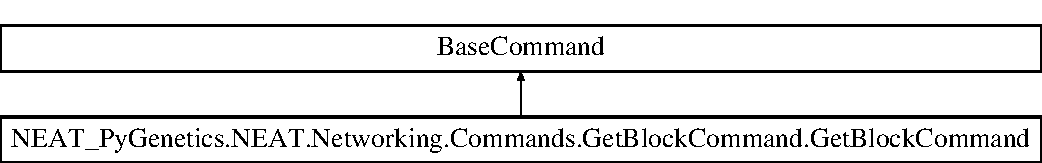
\includegraphics[height=2.000000cm]{classNEAT__PyGenetics_1_1NEAT_1_1Networking_1_1Commands_1_1GetBlockCommand_1_1GetBlockCommand}
\end{center}
\end{figure}
\subsection*{Public Member Functions}
\begin{DoxyCompactItemize}
\item 
def \hyperlink{classNEAT__PyGenetics_1_1NEAT_1_1Networking_1_1Commands_1_1GetBlockCommand_1_1GetBlockCommand_ad58e15de61d1576383f64ad5e99ab691}{\+\_\+\+\_\+init\+\_\+\+\_\+} (self)
\item 
def \hyperlink{classNEAT__PyGenetics_1_1NEAT_1_1Networking_1_1Commands_1_1GetBlockCommand_1_1GetBlockCommand_abd6d6e34fe53e47b6bd8fe3be8a38f6c}{set\+\_\+block\+\_\+id}
\item 
def \hyperlink{classNEAT__PyGenetics_1_1NEAT_1_1Networking_1_1Commands_1_1GetBlockCommand_1_1GetBlockCommand_af58224cb2bfb479548d3ec42cdee8931}{get\+\_\+block\+\_\+id} (self)
\item 
def \hyperlink{classNEAT__PyGenetics_1_1NEAT_1_1Networking_1_1Commands_1_1GetBlockCommand_1_1GetBlockCommand_a0a4947f054e52700ca72c6f9f6ece118}{get\+\_\+block} (self)
\item 
def \hyperlink{classNEAT__PyGenetics_1_1NEAT_1_1Networking_1_1Commands_1_1GetBlockCommand_1_1GetBlockCommand_a54eae8fc81e0a71fec523ce013637fc0}{get\+\_\+block\+\_\+size} (self)
\item 
def \hyperlink{classNEAT__PyGenetics_1_1NEAT_1_1Networking_1_1Commands_1_1GetBlockCommand_1_1GetBlockCommand_aabe6091c8da0ef7cc5655cbcd1b7ec5b}{get\+\_\+resulting\+\_\+block\+\_\+id} (self)
\item 
def \hyperlink{classNEAT__PyGenetics_1_1NEAT_1_1Networking_1_1Commands_1_1GetBlockCommand_1_1GetBlockCommand_a97eb16c91c2ebb7081518119585f55fe}{get\+\_\+next\+\_\+block\+\_\+id} (self)
\end{DoxyCompactItemize}


\subsection{Constructor \& Destructor Documentation}
\index{N\+E\+A\+T\+\_\+\+Py\+Genetics\+::\+N\+E\+A\+T\+::\+Networking\+::\+Commands\+::\+Get\+Block\+Command\+::\+Get\+Block\+Command@{N\+E\+A\+T\+\_\+\+Py\+Genetics\+::\+N\+E\+A\+T\+::\+Networking\+::\+Commands\+::\+Get\+Block\+Command\+::\+Get\+Block\+Command}!\+\_\+\+\_\+init\+\_\+\+\_\+@{\+\_\+\+\_\+init\+\_\+\+\_\+}}
\index{\+\_\+\+\_\+init\+\_\+\+\_\+@{\+\_\+\+\_\+init\+\_\+\+\_\+}!N\+E\+A\+T\+\_\+\+Py\+Genetics\+::\+N\+E\+A\+T\+::\+Networking\+::\+Commands\+::\+Get\+Block\+Command\+::\+Get\+Block\+Command@{N\+E\+A\+T\+\_\+\+Py\+Genetics\+::\+N\+E\+A\+T\+::\+Networking\+::\+Commands\+::\+Get\+Block\+Command\+::\+Get\+Block\+Command}}
\subsubsection[{\texorpdfstring{\+\_\+\+\_\+init\+\_\+\+\_\+(self)}{__init__(self)}}]{\setlength{\rightskip}{0pt plus 5cm}def N\+E\+A\+T\+\_\+\+Py\+Genetics.\+N\+E\+A\+T.\+Networking.\+Commands.\+Get\+Block\+Command.\+Get\+Block\+Command.\+\_\+\+\_\+init\+\_\+\+\_\+ (
\begin{DoxyParamCaption}
\item[{}]{self}
\end{DoxyParamCaption}
)}\hypertarget{classNEAT__PyGenetics_1_1NEAT_1_1Networking_1_1Commands_1_1GetBlockCommand_1_1GetBlockCommand_ad58e15de61d1576383f64ad5e99ab691}{}\label{classNEAT__PyGenetics_1_1NEAT_1_1Networking_1_1Commands_1_1GetBlockCommand_1_1GetBlockCommand_ad58e15de61d1576383f64ad5e99ab691}


\subsection{Member Function Documentation}
\index{N\+E\+A\+T\+\_\+\+Py\+Genetics\+::\+N\+E\+A\+T\+::\+Networking\+::\+Commands\+::\+Get\+Block\+Command\+::\+Get\+Block\+Command@{N\+E\+A\+T\+\_\+\+Py\+Genetics\+::\+N\+E\+A\+T\+::\+Networking\+::\+Commands\+::\+Get\+Block\+Command\+::\+Get\+Block\+Command}!get\+\_\+block@{get\+\_\+block}}
\index{get\+\_\+block@{get\+\_\+block}!N\+E\+A\+T\+\_\+\+Py\+Genetics\+::\+N\+E\+A\+T\+::\+Networking\+::\+Commands\+::\+Get\+Block\+Command\+::\+Get\+Block\+Command@{N\+E\+A\+T\+\_\+\+Py\+Genetics\+::\+N\+E\+A\+T\+::\+Networking\+::\+Commands\+::\+Get\+Block\+Command\+::\+Get\+Block\+Command}}
\subsubsection[{\texorpdfstring{get\+\_\+block(self)}{get_block(self)}}]{\setlength{\rightskip}{0pt plus 5cm}def N\+E\+A\+T\+\_\+\+Py\+Genetics.\+N\+E\+A\+T.\+Networking.\+Commands.\+Get\+Block\+Command.\+Get\+Block\+Command.\+get\+\_\+block (
\begin{DoxyParamCaption}
\item[{}]{self, }
\item[{}]{Dict, }
\item[{}]{Object\+Id, }
\item[{}]{Dict, }
\item[{}]{str, }
\item[{}]{float}
\end{DoxyParamCaption}
)}\hypertarget{classNEAT__PyGenetics_1_1NEAT_1_1Networking_1_1Commands_1_1GetBlockCommand_1_1GetBlockCommand_a0a4947f054e52700ca72c6f9f6ece118}{}\label{classNEAT__PyGenetics_1_1NEAT_1_1Networking_1_1Commands_1_1GetBlockCommand_1_1GetBlockCommand_a0a4947f054e52700ca72c6f9f6ece118}
\index{N\+E\+A\+T\+\_\+\+Py\+Genetics\+::\+N\+E\+A\+T\+::\+Networking\+::\+Commands\+::\+Get\+Block\+Command\+::\+Get\+Block\+Command@{N\+E\+A\+T\+\_\+\+Py\+Genetics\+::\+N\+E\+A\+T\+::\+Networking\+::\+Commands\+::\+Get\+Block\+Command\+::\+Get\+Block\+Command}!get\+\_\+block\+\_\+id@{get\+\_\+block\+\_\+id}}
\index{get\+\_\+block\+\_\+id@{get\+\_\+block\+\_\+id}!N\+E\+A\+T\+\_\+\+Py\+Genetics\+::\+N\+E\+A\+T\+::\+Networking\+::\+Commands\+::\+Get\+Block\+Command\+::\+Get\+Block\+Command@{N\+E\+A\+T\+\_\+\+Py\+Genetics\+::\+N\+E\+A\+T\+::\+Networking\+::\+Commands\+::\+Get\+Block\+Command\+::\+Get\+Block\+Command}}
\subsubsection[{\texorpdfstring{get\+\_\+block\+\_\+id(self)}{get_block_id(self)}}]{\setlength{\rightskip}{0pt plus 5cm}def N\+E\+A\+T\+\_\+\+Py\+Genetics.\+N\+E\+A\+T.\+Networking.\+Commands.\+Get\+Block\+Command.\+Get\+Block\+Command.\+get\+\_\+block\+\_\+id (
\begin{DoxyParamCaption}
\item[{}]{self}
\end{DoxyParamCaption}
)}\hypertarget{classNEAT__PyGenetics_1_1NEAT_1_1Networking_1_1Commands_1_1GetBlockCommand_1_1GetBlockCommand_af58224cb2bfb479548d3ec42cdee8931}{}\label{classNEAT__PyGenetics_1_1NEAT_1_1Networking_1_1Commands_1_1GetBlockCommand_1_1GetBlockCommand_af58224cb2bfb479548d3ec42cdee8931}
\index{N\+E\+A\+T\+\_\+\+Py\+Genetics\+::\+N\+E\+A\+T\+::\+Networking\+::\+Commands\+::\+Get\+Block\+Command\+::\+Get\+Block\+Command@{N\+E\+A\+T\+\_\+\+Py\+Genetics\+::\+N\+E\+A\+T\+::\+Networking\+::\+Commands\+::\+Get\+Block\+Command\+::\+Get\+Block\+Command}!get\+\_\+block\+\_\+size@{get\+\_\+block\+\_\+size}}
\index{get\+\_\+block\+\_\+size@{get\+\_\+block\+\_\+size}!N\+E\+A\+T\+\_\+\+Py\+Genetics\+::\+N\+E\+A\+T\+::\+Networking\+::\+Commands\+::\+Get\+Block\+Command\+::\+Get\+Block\+Command@{N\+E\+A\+T\+\_\+\+Py\+Genetics\+::\+N\+E\+A\+T\+::\+Networking\+::\+Commands\+::\+Get\+Block\+Command\+::\+Get\+Block\+Command}}
\subsubsection[{\texorpdfstring{get\+\_\+block\+\_\+size(self)}{get_block_size(self)}}]{\setlength{\rightskip}{0pt plus 5cm}def N\+E\+A\+T\+\_\+\+Py\+Genetics.\+N\+E\+A\+T.\+Networking.\+Commands.\+Get\+Block\+Command.\+Get\+Block\+Command.\+get\+\_\+block\+\_\+size (
\begin{DoxyParamCaption}
\item[{}]{self, }
\item[{}]{int}
\end{DoxyParamCaption}
)}\hypertarget{classNEAT__PyGenetics_1_1NEAT_1_1Networking_1_1Commands_1_1GetBlockCommand_1_1GetBlockCommand_a54eae8fc81e0a71fec523ce013637fc0}{}\label{classNEAT__PyGenetics_1_1NEAT_1_1Networking_1_1Commands_1_1GetBlockCommand_1_1GetBlockCommand_a54eae8fc81e0a71fec523ce013637fc0}
\index{N\+E\+A\+T\+\_\+\+Py\+Genetics\+::\+N\+E\+A\+T\+::\+Networking\+::\+Commands\+::\+Get\+Block\+Command\+::\+Get\+Block\+Command@{N\+E\+A\+T\+\_\+\+Py\+Genetics\+::\+N\+E\+A\+T\+::\+Networking\+::\+Commands\+::\+Get\+Block\+Command\+::\+Get\+Block\+Command}!get\+\_\+next\+\_\+block\+\_\+id@{get\+\_\+next\+\_\+block\+\_\+id}}
\index{get\+\_\+next\+\_\+block\+\_\+id@{get\+\_\+next\+\_\+block\+\_\+id}!N\+E\+A\+T\+\_\+\+Py\+Genetics\+::\+N\+E\+A\+T\+::\+Networking\+::\+Commands\+::\+Get\+Block\+Command\+::\+Get\+Block\+Command@{N\+E\+A\+T\+\_\+\+Py\+Genetics\+::\+N\+E\+A\+T\+::\+Networking\+::\+Commands\+::\+Get\+Block\+Command\+::\+Get\+Block\+Command}}
\subsubsection[{\texorpdfstring{get\+\_\+next\+\_\+block\+\_\+id(self)}{get_next_block_id(self)}}]{\setlength{\rightskip}{0pt plus 5cm}def N\+E\+A\+T\+\_\+\+Py\+Genetics.\+N\+E\+A\+T.\+Networking.\+Commands.\+Get\+Block\+Command.\+Get\+Block\+Command.\+get\+\_\+next\+\_\+block\+\_\+id (
\begin{DoxyParamCaption}
\item[{}]{self, }
\item[{}]{int}
\end{DoxyParamCaption}
)}\hypertarget{classNEAT__PyGenetics_1_1NEAT_1_1Networking_1_1Commands_1_1GetBlockCommand_1_1GetBlockCommand_a97eb16c91c2ebb7081518119585f55fe}{}\label{classNEAT__PyGenetics_1_1NEAT_1_1Networking_1_1Commands_1_1GetBlockCommand_1_1GetBlockCommand_a97eb16c91c2ebb7081518119585f55fe}
\index{N\+E\+A\+T\+\_\+\+Py\+Genetics\+::\+N\+E\+A\+T\+::\+Networking\+::\+Commands\+::\+Get\+Block\+Command\+::\+Get\+Block\+Command@{N\+E\+A\+T\+\_\+\+Py\+Genetics\+::\+N\+E\+A\+T\+::\+Networking\+::\+Commands\+::\+Get\+Block\+Command\+::\+Get\+Block\+Command}!get\+\_\+resulting\+\_\+block\+\_\+id@{get\+\_\+resulting\+\_\+block\+\_\+id}}
\index{get\+\_\+resulting\+\_\+block\+\_\+id@{get\+\_\+resulting\+\_\+block\+\_\+id}!N\+E\+A\+T\+\_\+\+Py\+Genetics\+::\+N\+E\+A\+T\+::\+Networking\+::\+Commands\+::\+Get\+Block\+Command\+::\+Get\+Block\+Command@{N\+E\+A\+T\+\_\+\+Py\+Genetics\+::\+N\+E\+A\+T\+::\+Networking\+::\+Commands\+::\+Get\+Block\+Command\+::\+Get\+Block\+Command}}
\subsubsection[{\texorpdfstring{get\+\_\+resulting\+\_\+block\+\_\+id(self)}{get_resulting_block_id(self)}}]{\setlength{\rightskip}{0pt plus 5cm}def N\+E\+A\+T\+\_\+\+Py\+Genetics.\+N\+E\+A\+T.\+Networking.\+Commands.\+Get\+Block\+Command.\+Get\+Block\+Command.\+get\+\_\+resulting\+\_\+block\+\_\+id (
\begin{DoxyParamCaption}
\item[{}]{self, }
\item[{}]{int}
\end{DoxyParamCaption}
)}\hypertarget{classNEAT__PyGenetics_1_1NEAT_1_1Networking_1_1Commands_1_1GetBlockCommand_1_1GetBlockCommand_aabe6091c8da0ef7cc5655cbcd1b7ec5b}{}\label{classNEAT__PyGenetics_1_1NEAT_1_1Networking_1_1Commands_1_1GetBlockCommand_1_1GetBlockCommand_aabe6091c8da0ef7cc5655cbcd1b7ec5b}
\index{N\+E\+A\+T\+\_\+\+Py\+Genetics\+::\+N\+E\+A\+T\+::\+Networking\+::\+Commands\+::\+Get\+Block\+Command\+::\+Get\+Block\+Command@{N\+E\+A\+T\+\_\+\+Py\+Genetics\+::\+N\+E\+A\+T\+::\+Networking\+::\+Commands\+::\+Get\+Block\+Command\+::\+Get\+Block\+Command}!set\+\_\+block\+\_\+id@{set\+\_\+block\+\_\+id}}
\index{set\+\_\+block\+\_\+id@{set\+\_\+block\+\_\+id}!N\+E\+A\+T\+\_\+\+Py\+Genetics\+::\+N\+E\+A\+T\+::\+Networking\+::\+Commands\+::\+Get\+Block\+Command\+::\+Get\+Block\+Command@{N\+E\+A\+T\+\_\+\+Py\+Genetics\+::\+N\+E\+A\+T\+::\+Networking\+::\+Commands\+::\+Get\+Block\+Command\+::\+Get\+Block\+Command}}
\subsubsection[{\texorpdfstring{set\+\_\+block\+\_\+id}{set_block_id}}]{\setlength{\rightskip}{0pt plus 5cm}def N\+E\+A\+T\+\_\+\+Py\+Genetics.\+N\+E\+A\+T.\+Networking.\+Commands.\+Get\+Block\+Command.\+Get\+Block\+Command.\+set\+\_\+block\+\_\+id (
\begin{DoxyParamCaption}
\item[{}]{self, }
\item[{}]{block\+\_\+id}
\end{DoxyParamCaption}
)}\hypertarget{classNEAT__PyGenetics_1_1NEAT_1_1Networking_1_1Commands_1_1GetBlockCommand_1_1GetBlockCommand_abd6d6e34fe53e47b6bd8fe3be8a38f6c}{}\label{classNEAT__PyGenetics_1_1NEAT_1_1Networking_1_1Commands_1_1GetBlockCommand_1_1GetBlockCommand_abd6d6e34fe53e47b6bd8fe3be8a38f6c}


The documentation for this class was generated from the following file\+:\begin{DoxyCompactItemize}
\item 
N\+E\+A\+T/\+Networking/\+Commands/\hyperlink{GetBlockCommand_8py}{Get\+Block\+Command.\+py}\end{DoxyCompactItemize}

\hypertarget{classNEAT__PyGenetics_1_1NEAT_1_1Networking_1_1Commands_1_1GetOutputsCommand_1_1GetOutputsCommand}{}\section{N\+E\+A\+T\+\_\+\+Py\+Genetics.\+N\+E\+A\+T.\+Networking.\+Commands.\+Get\+Outputs\+Command.\+Get\+Outputs\+Command Class Reference}
\label{classNEAT__PyGenetics_1_1NEAT_1_1Networking_1_1Commands_1_1GetOutputsCommand_1_1GetOutputsCommand}\index{N\+E\+A\+T\+\_\+\+Py\+Genetics.\+N\+E\+A\+T.\+Networking.\+Commands.\+Get\+Outputs\+Command.\+Get\+Outputs\+Command@{N\+E\+A\+T\+\_\+\+Py\+Genetics.\+N\+E\+A\+T.\+Networking.\+Commands.\+Get\+Outputs\+Command.\+Get\+Outputs\+Command}}
Inheritance diagram for N\+E\+A\+T\+\_\+\+Py\+Genetics.\+N\+E\+A\+T.\+Networking.\+Commands.\+Get\+Outputs\+Command.\+Get\+Outputs\+Command\+:\begin{figure}[H]
\begin{center}
\leavevmode
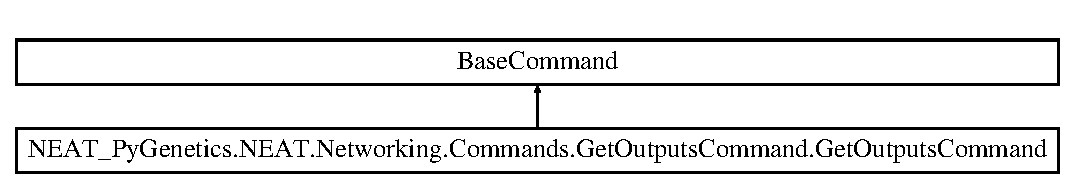
\includegraphics[height=2.000000cm]{classNEAT__PyGenetics_1_1NEAT_1_1Networking_1_1Commands_1_1GetOutputsCommand_1_1GetOutputsCommand}
\end{center}
\end{figure}
\subsection*{Public Member Functions}
\begin{DoxyCompactItemize}
\item 
def \hyperlink{classNEAT__PyGenetics_1_1NEAT_1_1Networking_1_1Commands_1_1GetOutputsCommand_1_1GetOutputsCommand_a9cb7b34e60b60ab5b71843ba223ff626}{\+\_\+\+\_\+init\+\_\+\+\_\+} (self)
\item 
def \hyperlink{classNEAT__PyGenetics_1_1NEAT_1_1Networking_1_1Commands_1_1GetOutputsCommand_1_1GetOutputsCommand_a8ec7f2dc4780ec36b72c7fbff9492621}{set\+\_\+block\+\_\+id}
\item 
def \hyperlink{classNEAT__PyGenetics_1_1NEAT_1_1Networking_1_1Commands_1_1GetOutputsCommand_1_1GetOutputsCommand_af1c805c74a7c01ff8314f84f8461f25c}{get\+\_\+block\+\_\+id} (self)
\end{DoxyCompactItemize}


\subsection{Constructor \& Destructor Documentation}
\index{N\+E\+A\+T\+\_\+\+Py\+Genetics\+::\+N\+E\+A\+T\+::\+Networking\+::\+Commands\+::\+Get\+Outputs\+Command\+::\+Get\+Outputs\+Command@{N\+E\+A\+T\+\_\+\+Py\+Genetics\+::\+N\+E\+A\+T\+::\+Networking\+::\+Commands\+::\+Get\+Outputs\+Command\+::\+Get\+Outputs\+Command}!\+\_\+\+\_\+init\+\_\+\+\_\+@{\+\_\+\+\_\+init\+\_\+\+\_\+}}
\index{\+\_\+\+\_\+init\+\_\+\+\_\+@{\+\_\+\+\_\+init\+\_\+\+\_\+}!N\+E\+A\+T\+\_\+\+Py\+Genetics\+::\+N\+E\+A\+T\+::\+Networking\+::\+Commands\+::\+Get\+Outputs\+Command\+::\+Get\+Outputs\+Command@{N\+E\+A\+T\+\_\+\+Py\+Genetics\+::\+N\+E\+A\+T\+::\+Networking\+::\+Commands\+::\+Get\+Outputs\+Command\+::\+Get\+Outputs\+Command}}
\subsubsection[{\texorpdfstring{\+\_\+\+\_\+init\+\_\+\+\_\+(self)}{__init__(self)}}]{\setlength{\rightskip}{0pt plus 5cm}def N\+E\+A\+T\+\_\+\+Py\+Genetics.\+N\+E\+A\+T.\+Networking.\+Commands.\+Get\+Outputs\+Command.\+Get\+Outputs\+Command.\+\_\+\+\_\+init\+\_\+\+\_\+ (
\begin{DoxyParamCaption}
\item[{}]{self}
\end{DoxyParamCaption}
)}\hypertarget{classNEAT__PyGenetics_1_1NEAT_1_1Networking_1_1Commands_1_1GetOutputsCommand_1_1GetOutputsCommand_a9cb7b34e60b60ab5b71843ba223ff626}{}\label{classNEAT__PyGenetics_1_1NEAT_1_1Networking_1_1Commands_1_1GetOutputsCommand_1_1GetOutputsCommand_a9cb7b34e60b60ab5b71843ba223ff626}


\subsection{Member Function Documentation}
\index{N\+E\+A\+T\+\_\+\+Py\+Genetics\+::\+N\+E\+A\+T\+::\+Networking\+::\+Commands\+::\+Get\+Outputs\+Command\+::\+Get\+Outputs\+Command@{N\+E\+A\+T\+\_\+\+Py\+Genetics\+::\+N\+E\+A\+T\+::\+Networking\+::\+Commands\+::\+Get\+Outputs\+Command\+::\+Get\+Outputs\+Command}!get\+\_\+block\+\_\+id@{get\+\_\+block\+\_\+id}}
\index{get\+\_\+block\+\_\+id@{get\+\_\+block\+\_\+id}!N\+E\+A\+T\+\_\+\+Py\+Genetics\+::\+N\+E\+A\+T\+::\+Networking\+::\+Commands\+::\+Get\+Outputs\+Command\+::\+Get\+Outputs\+Command@{N\+E\+A\+T\+\_\+\+Py\+Genetics\+::\+N\+E\+A\+T\+::\+Networking\+::\+Commands\+::\+Get\+Outputs\+Command\+::\+Get\+Outputs\+Command}}
\subsubsection[{\texorpdfstring{get\+\_\+block\+\_\+id(self)}{get_block_id(self)}}]{\setlength{\rightskip}{0pt plus 5cm}def N\+E\+A\+T\+\_\+\+Py\+Genetics.\+N\+E\+A\+T.\+Networking.\+Commands.\+Get\+Outputs\+Command.\+Get\+Outputs\+Command.\+get\+\_\+block\+\_\+id (
\begin{DoxyParamCaption}
\item[{}]{self}
\end{DoxyParamCaption}
)}\hypertarget{classNEAT__PyGenetics_1_1NEAT_1_1Networking_1_1Commands_1_1GetOutputsCommand_1_1GetOutputsCommand_af1c805c74a7c01ff8314f84f8461f25c}{}\label{classNEAT__PyGenetics_1_1NEAT_1_1Networking_1_1Commands_1_1GetOutputsCommand_1_1GetOutputsCommand_af1c805c74a7c01ff8314f84f8461f25c}
\index{N\+E\+A\+T\+\_\+\+Py\+Genetics\+::\+N\+E\+A\+T\+::\+Networking\+::\+Commands\+::\+Get\+Outputs\+Command\+::\+Get\+Outputs\+Command@{N\+E\+A\+T\+\_\+\+Py\+Genetics\+::\+N\+E\+A\+T\+::\+Networking\+::\+Commands\+::\+Get\+Outputs\+Command\+::\+Get\+Outputs\+Command}!set\+\_\+block\+\_\+id@{set\+\_\+block\+\_\+id}}
\index{set\+\_\+block\+\_\+id@{set\+\_\+block\+\_\+id}!N\+E\+A\+T\+\_\+\+Py\+Genetics\+::\+N\+E\+A\+T\+::\+Networking\+::\+Commands\+::\+Get\+Outputs\+Command\+::\+Get\+Outputs\+Command@{N\+E\+A\+T\+\_\+\+Py\+Genetics\+::\+N\+E\+A\+T\+::\+Networking\+::\+Commands\+::\+Get\+Outputs\+Command\+::\+Get\+Outputs\+Command}}
\subsubsection[{\texorpdfstring{set\+\_\+block\+\_\+id}{set_block_id}}]{\setlength{\rightskip}{0pt plus 5cm}def N\+E\+A\+T\+\_\+\+Py\+Genetics.\+N\+E\+A\+T.\+Networking.\+Commands.\+Get\+Outputs\+Command.\+Get\+Outputs\+Command.\+set\+\_\+block\+\_\+id (
\begin{DoxyParamCaption}
\item[{}]{self, }
\item[{}]{block\+\_\+id}
\end{DoxyParamCaption}
)}\hypertarget{classNEAT__PyGenetics_1_1NEAT_1_1Networking_1_1Commands_1_1GetOutputsCommand_1_1GetOutputsCommand_a8ec7f2dc4780ec36b72c7fbff9492621}{}\label{classNEAT__PyGenetics_1_1NEAT_1_1Networking_1_1Commands_1_1GetOutputsCommand_1_1GetOutputsCommand_a8ec7f2dc4780ec36b72c7fbff9492621}


The documentation for this class was generated from the following file\+:\begin{DoxyCompactItemize}
\item 
N\+E\+A\+T/\+Networking/\+Commands/\hyperlink{GetOutputsCommand_8py}{Get\+Outputs\+Command.\+py}\end{DoxyCompactItemize}

\hypertarget{classNEAT__PyGenetics_1_1NEAT_1_1ErrorHandling_1_1Exceptions_1_1InputMissingException_1_1InputMissingException}{}\section{N\+E\+A\+T\+\_\+\+Py\+Genetics.\+N\+E\+A\+T.\+Error\+Handling.\+Exceptions.\+Input\+Missing\+Exception.\+Input\+Missing\+Exception Class Reference}
\label{classNEAT__PyGenetics_1_1NEAT_1_1ErrorHandling_1_1Exceptions_1_1InputMissingException_1_1InputMissingException}\index{N\+E\+A\+T\+\_\+\+Py\+Genetics.\+N\+E\+A\+T.\+Error\+Handling.\+Exceptions.\+Input\+Missing\+Exception.\+Input\+Missing\+Exception@{N\+E\+A\+T\+\_\+\+Py\+Genetics.\+N\+E\+A\+T.\+Error\+Handling.\+Exceptions.\+Input\+Missing\+Exception.\+Input\+Missing\+Exception}}
Inheritance diagram for N\+E\+A\+T\+\_\+\+Py\+Genetics.\+N\+E\+A\+T.\+Error\+Handling.\+Exceptions.\+Input\+Missing\+Exception.\+Input\+Missing\+Exception\+:\begin{figure}[H]
\begin{center}
\leavevmode
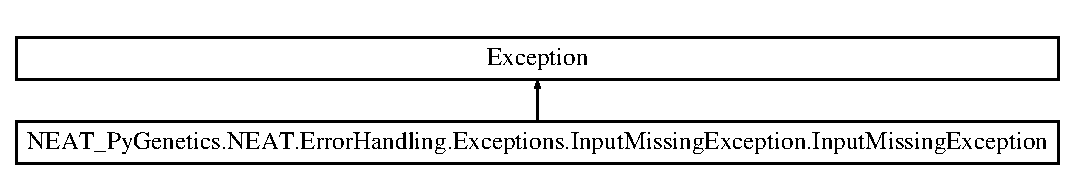
\includegraphics[height=1.971831cm]{classNEAT__PyGenetics_1_1NEAT_1_1ErrorHandling_1_1Exceptions_1_1InputMissingException_1_1InputMissingException}
\end{center}
\end{figure}
\subsection*{Public Member Functions}
\begin{DoxyCompactItemize}
\item 
def \hyperlink{classNEAT__PyGenetics_1_1NEAT_1_1ErrorHandling_1_1Exceptions_1_1InputMissingException_1_1InputMissingException_ad099b1a8bf35220cc7d2a47d4469d749}{\+\_\+\+\_\+init\+\_\+\+\_\+} (self, message, errors=None)
\end{DoxyCompactItemize}


\subsection{Constructor \& Destructor Documentation}
\index{N\+E\+A\+T\+\_\+\+Py\+Genetics\+::\+N\+E\+A\+T\+::\+Error\+Handling\+::\+Exceptions\+::\+Input\+Missing\+Exception\+::\+Input\+Missing\+Exception@{N\+E\+A\+T\+\_\+\+Py\+Genetics\+::\+N\+E\+A\+T\+::\+Error\+Handling\+::\+Exceptions\+::\+Input\+Missing\+Exception\+::\+Input\+Missing\+Exception}!\+\_\+\+\_\+init\+\_\+\+\_\+@{\+\_\+\+\_\+init\+\_\+\+\_\+}}
\index{\+\_\+\+\_\+init\+\_\+\+\_\+@{\+\_\+\+\_\+init\+\_\+\+\_\+}!N\+E\+A\+T\+\_\+\+Py\+Genetics\+::\+N\+E\+A\+T\+::\+Error\+Handling\+::\+Exceptions\+::\+Input\+Missing\+Exception\+::\+Input\+Missing\+Exception@{N\+E\+A\+T\+\_\+\+Py\+Genetics\+::\+N\+E\+A\+T\+::\+Error\+Handling\+::\+Exceptions\+::\+Input\+Missing\+Exception\+::\+Input\+Missing\+Exception}}
\subsubsection[{\texorpdfstring{\+\_\+\+\_\+init\+\_\+\+\_\+(self, message, errors=\+None)}{__init__(self, message, errors=None)}}]{\setlength{\rightskip}{0pt plus 5cm}def N\+E\+A\+T\+\_\+\+Py\+Genetics.\+N\+E\+A\+T.\+Error\+Handling.\+Exceptions.\+Input\+Missing\+Exception.\+Input\+Missing\+Exception.\+\_\+\+\_\+init\+\_\+\+\_\+ (
\begin{DoxyParamCaption}
\item[{}]{self, }
\item[{}]{message, }
\item[{}]{errors = {\ttfamily None}}
\end{DoxyParamCaption}
)}\hypertarget{classNEAT__PyGenetics_1_1NEAT_1_1ErrorHandling_1_1Exceptions_1_1InputMissingException_1_1InputMissingException_ad099b1a8bf35220cc7d2a47d4469d749}{}\label{classNEAT__PyGenetics_1_1NEAT_1_1ErrorHandling_1_1Exceptions_1_1InputMissingException_1_1InputMissingException_ad099b1a8bf35220cc7d2a47d4469d749}


The documentation for this class was generated from the following file\+:\begin{DoxyCompactItemize}
\item 
N\+E\+A\+T/\+Error\+Handling/\+Exceptions/\hyperlink{InputMissingException_8py}{Input\+Missing\+Exception.\+py}\end{DoxyCompactItemize}

\hypertarget{classNEAT__PyGenetics_1_1NEAT_1_1Networking_1_1Server_1_1JSONSocket_1_1JSONSocket}{}\section{N\+E\+A\+T\+\_\+\+Py\+Genetics.\+N\+E\+A\+T.\+Networking.\+Server.\+J\+S\+O\+N\+Socket.\+J\+S\+O\+N\+Socket Class Reference}
\label{classNEAT__PyGenetics_1_1NEAT_1_1Networking_1_1Server_1_1JSONSocket_1_1JSONSocket}\index{N\+E\+A\+T\+\_\+\+Py\+Genetics.\+N\+E\+A\+T.\+Networking.\+Server.\+J\+S\+O\+N\+Socket.\+J\+S\+O\+N\+Socket@{N\+E\+A\+T\+\_\+\+Py\+Genetics.\+N\+E\+A\+T.\+Networking.\+Server.\+J\+S\+O\+N\+Socket.\+J\+S\+O\+N\+Socket}}
Inheritance diagram for N\+E\+A\+T\+\_\+\+Py\+Genetics.\+N\+E\+A\+T.\+Networking.\+Server.\+J\+S\+O\+N\+Socket.\+J\+S\+O\+N\+Socket\+:\begin{figure}[H]
\begin{center}
\leavevmode
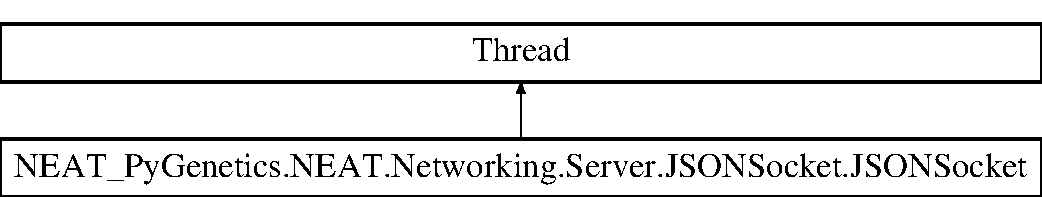
\includegraphics[height=2.000000cm]{classNEAT__PyGenetics_1_1NEAT_1_1Networking_1_1Server_1_1JSONSocket_1_1JSONSocket}
\end{center}
\end{figure}
\subsection*{Public Member Functions}
\begin{DoxyCompactItemize}
\item 
def \hyperlink{classNEAT__PyGenetics_1_1NEAT_1_1Networking_1_1Server_1_1JSONSocket_1_1JSONSocket_a95dd555e4124ce36a47d00e3b62b597a}{\+\_\+\+\_\+init\+\_\+\+\_\+} (self, server\+\_\+address, server\+\_\+port, header\+\_\+size=16, chunk\+\_\+size=1024)
\item 
def \hyperlink{classNEAT__PyGenetics_1_1NEAT_1_1Networking_1_1Server_1_1JSONSocket_1_1JSONSocket_a05c99b2b4e7b4552155560f5fad0b939}{socket\+\_\+alive} (self)
\item 
def \hyperlink{classNEAT__PyGenetics_1_1NEAT_1_1Networking_1_1Server_1_1JSONSocket_1_1JSONSocket_a196c88e61cbc698f1012a5561f85f6d0}{close\+\_\+connection} (self)
\item 
def \hyperlink{classNEAT__PyGenetics_1_1NEAT_1_1Networking_1_1Server_1_1JSONSocket_1_1JSONSocket_a104209f938a7b47d91692face1dc0569}{send\+\_\+dict}
\item 
def \hyperlink{classNEAT__PyGenetics_1_1NEAT_1_1Networking_1_1Server_1_1JSONSocket_1_1JSONSocket_a2bc8b4e45a2e94d386c98caba0ecce14}{receive\+\_\+dict} (self)
\end{DoxyCompactItemize}


\subsection{Constructor \& Destructor Documentation}
\index{N\+E\+A\+T\+\_\+\+Py\+Genetics\+::\+N\+E\+A\+T\+::\+Networking\+::\+Server\+::\+J\+S\+O\+N\+Socket\+::\+J\+S\+O\+N\+Socket@{N\+E\+A\+T\+\_\+\+Py\+Genetics\+::\+N\+E\+A\+T\+::\+Networking\+::\+Server\+::\+J\+S\+O\+N\+Socket\+::\+J\+S\+O\+N\+Socket}!\+\_\+\+\_\+init\+\_\+\+\_\+@{\+\_\+\+\_\+init\+\_\+\+\_\+}}
\index{\+\_\+\+\_\+init\+\_\+\+\_\+@{\+\_\+\+\_\+init\+\_\+\+\_\+}!N\+E\+A\+T\+\_\+\+Py\+Genetics\+::\+N\+E\+A\+T\+::\+Networking\+::\+Server\+::\+J\+S\+O\+N\+Socket\+::\+J\+S\+O\+N\+Socket@{N\+E\+A\+T\+\_\+\+Py\+Genetics\+::\+N\+E\+A\+T\+::\+Networking\+::\+Server\+::\+J\+S\+O\+N\+Socket\+::\+J\+S\+O\+N\+Socket}}
\subsubsection[{\texorpdfstring{\+\_\+\+\_\+init\+\_\+\+\_\+(self, server\+\_\+address, server\+\_\+port, header\+\_\+size=16, chunk\+\_\+size=1024)}{__init__(self, server_address, server_port, header_size=16, chunk_size=1024)}}]{\setlength{\rightskip}{0pt plus 5cm}def N\+E\+A\+T\+\_\+\+Py\+Genetics.\+N\+E\+A\+T.\+Networking.\+Server.\+J\+S\+O\+N\+Socket.\+J\+S\+O\+N\+Socket.\+\_\+\+\_\+init\+\_\+\+\_\+ (
\begin{DoxyParamCaption}
\item[{}]{self, }
\item[{}]{server\+\_\+address, }
\item[{}]{server\+\_\+port, }
\item[{}]{header\+\_\+size = {\ttfamily 16}, }
\item[{}]{chunk\+\_\+size = {\ttfamily 1024}}
\end{DoxyParamCaption}
)}\hypertarget{classNEAT__PyGenetics_1_1NEAT_1_1Networking_1_1Server_1_1JSONSocket_1_1JSONSocket_a95dd555e4124ce36a47d00e3b62b597a}{}\label{classNEAT__PyGenetics_1_1NEAT_1_1Networking_1_1Server_1_1JSONSocket_1_1JSONSocket_a95dd555e4124ce36a47d00e3b62b597a}


\subsection{Member Function Documentation}
\index{N\+E\+A\+T\+\_\+\+Py\+Genetics\+::\+N\+E\+A\+T\+::\+Networking\+::\+Server\+::\+J\+S\+O\+N\+Socket\+::\+J\+S\+O\+N\+Socket@{N\+E\+A\+T\+\_\+\+Py\+Genetics\+::\+N\+E\+A\+T\+::\+Networking\+::\+Server\+::\+J\+S\+O\+N\+Socket\+::\+J\+S\+O\+N\+Socket}!close\+\_\+connection@{close\+\_\+connection}}
\index{close\+\_\+connection@{close\+\_\+connection}!N\+E\+A\+T\+\_\+\+Py\+Genetics\+::\+N\+E\+A\+T\+::\+Networking\+::\+Server\+::\+J\+S\+O\+N\+Socket\+::\+J\+S\+O\+N\+Socket@{N\+E\+A\+T\+\_\+\+Py\+Genetics\+::\+N\+E\+A\+T\+::\+Networking\+::\+Server\+::\+J\+S\+O\+N\+Socket\+::\+J\+S\+O\+N\+Socket}}
\subsubsection[{\texorpdfstring{close\+\_\+connection(self)}{close_connection(self)}}]{\setlength{\rightskip}{0pt plus 5cm}def N\+E\+A\+T\+\_\+\+Py\+Genetics.\+N\+E\+A\+T.\+Networking.\+Server.\+J\+S\+O\+N\+Socket.\+J\+S\+O\+N\+Socket.\+close\+\_\+connection (
\begin{DoxyParamCaption}
\item[{}]{self, }
\item[{}]{None}
\end{DoxyParamCaption}
)}\hypertarget{classNEAT__PyGenetics_1_1NEAT_1_1Networking_1_1Server_1_1JSONSocket_1_1JSONSocket_a196c88e61cbc698f1012a5561f85f6d0}{}\label{classNEAT__PyGenetics_1_1NEAT_1_1Networking_1_1Server_1_1JSONSocket_1_1JSONSocket_a196c88e61cbc698f1012a5561f85f6d0}
\index{N\+E\+A\+T\+\_\+\+Py\+Genetics\+::\+N\+E\+A\+T\+::\+Networking\+::\+Server\+::\+J\+S\+O\+N\+Socket\+::\+J\+S\+O\+N\+Socket@{N\+E\+A\+T\+\_\+\+Py\+Genetics\+::\+N\+E\+A\+T\+::\+Networking\+::\+Server\+::\+J\+S\+O\+N\+Socket\+::\+J\+S\+O\+N\+Socket}!receive\+\_\+dict@{receive\+\_\+dict}}
\index{receive\+\_\+dict@{receive\+\_\+dict}!N\+E\+A\+T\+\_\+\+Py\+Genetics\+::\+N\+E\+A\+T\+::\+Networking\+::\+Server\+::\+J\+S\+O\+N\+Socket\+::\+J\+S\+O\+N\+Socket@{N\+E\+A\+T\+\_\+\+Py\+Genetics\+::\+N\+E\+A\+T\+::\+Networking\+::\+Server\+::\+J\+S\+O\+N\+Socket\+::\+J\+S\+O\+N\+Socket}}
\subsubsection[{\texorpdfstring{receive\+\_\+dict(self)}{receive_dict(self)}}]{\setlength{\rightskip}{0pt plus 5cm}def N\+E\+A\+T\+\_\+\+Py\+Genetics.\+N\+E\+A\+T.\+Networking.\+Server.\+J\+S\+O\+N\+Socket.\+J\+S\+O\+N\+Socket.\+receive\+\_\+dict (
\begin{DoxyParamCaption}
\item[{}]{self}
\end{DoxyParamCaption}
)}\hypertarget{classNEAT__PyGenetics_1_1NEAT_1_1Networking_1_1Server_1_1JSONSocket_1_1JSONSocket_a2bc8b4e45a2e94d386c98caba0ecce14}{}\label{classNEAT__PyGenetics_1_1NEAT_1_1Networking_1_1Server_1_1JSONSocket_1_1JSONSocket_a2bc8b4e45a2e94d386c98caba0ecce14}
\index{N\+E\+A\+T\+\_\+\+Py\+Genetics\+::\+N\+E\+A\+T\+::\+Networking\+::\+Server\+::\+J\+S\+O\+N\+Socket\+::\+J\+S\+O\+N\+Socket@{N\+E\+A\+T\+\_\+\+Py\+Genetics\+::\+N\+E\+A\+T\+::\+Networking\+::\+Server\+::\+J\+S\+O\+N\+Socket\+::\+J\+S\+O\+N\+Socket}!send\+\_\+dict@{send\+\_\+dict}}
\index{send\+\_\+dict@{send\+\_\+dict}!N\+E\+A\+T\+\_\+\+Py\+Genetics\+::\+N\+E\+A\+T\+::\+Networking\+::\+Server\+::\+J\+S\+O\+N\+Socket\+::\+J\+S\+O\+N\+Socket@{N\+E\+A\+T\+\_\+\+Py\+Genetics\+::\+N\+E\+A\+T\+::\+Networking\+::\+Server\+::\+J\+S\+O\+N\+Socket\+::\+J\+S\+O\+N\+Socket}}
\subsubsection[{\texorpdfstring{send\+\_\+dict}{send_dict}}]{\setlength{\rightskip}{0pt plus 5cm}def N\+E\+A\+T\+\_\+\+Py\+Genetics.\+N\+E\+A\+T.\+Networking.\+Server.\+J\+S\+O\+N\+Socket.\+J\+S\+O\+N\+Socket.\+send\+\_\+dict (
\begin{DoxyParamCaption}
\item[{}]{self, }
\item[{}]{dictionary}
\end{DoxyParamCaption}
)}\hypertarget{classNEAT__PyGenetics_1_1NEAT_1_1Networking_1_1Server_1_1JSONSocket_1_1JSONSocket_a104209f938a7b47d91692face1dc0569}{}\label{classNEAT__PyGenetics_1_1NEAT_1_1Networking_1_1Server_1_1JSONSocket_1_1JSONSocket_a104209f938a7b47d91692face1dc0569}
\index{N\+E\+A\+T\+\_\+\+Py\+Genetics\+::\+N\+E\+A\+T\+::\+Networking\+::\+Server\+::\+J\+S\+O\+N\+Socket\+::\+J\+S\+O\+N\+Socket@{N\+E\+A\+T\+\_\+\+Py\+Genetics\+::\+N\+E\+A\+T\+::\+Networking\+::\+Server\+::\+J\+S\+O\+N\+Socket\+::\+J\+S\+O\+N\+Socket}!socket\+\_\+alive@{socket\+\_\+alive}}
\index{socket\+\_\+alive@{socket\+\_\+alive}!N\+E\+A\+T\+\_\+\+Py\+Genetics\+::\+N\+E\+A\+T\+::\+Networking\+::\+Server\+::\+J\+S\+O\+N\+Socket\+::\+J\+S\+O\+N\+Socket@{N\+E\+A\+T\+\_\+\+Py\+Genetics\+::\+N\+E\+A\+T\+::\+Networking\+::\+Server\+::\+J\+S\+O\+N\+Socket\+::\+J\+S\+O\+N\+Socket}}
\subsubsection[{\texorpdfstring{socket\+\_\+alive(self)}{socket_alive(self)}}]{\setlength{\rightskip}{0pt plus 5cm}def N\+E\+A\+T\+\_\+\+Py\+Genetics.\+N\+E\+A\+T.\+Networking.\+Server.\+J\+S\+O\+N\+Socket.\+J\+S\+O\+N\+Socket.\+socket\+\_\+alive (
\begin{DoxyParamCaption}
\item[{}]{self, }
\item[{}]{bool}
\end{DoxyParamCaption}
)}\hypertarget{classNEAT__PyGenetics_1_1NEAT_1_1Networking_1_1Server_1_1JSONSocket_1_1JSONSocket_a05c99b2b4e7b4552155560f5fad0b939}{}\label{classNEAT__PyGenetics_1_1NEAT_1_1Networking_1_1Server_1_1JSONSocket_1_1JSONSocket_a05c99b2b4e7b4552155560f5fad0b939}


The documentation for this class was generated from the following file\+:\begin{DoxyCompactItemize}
\item 
N\+E\+A\+T/\+Networking/\+Server/\hyperlink{JSONSocket_8py}{J\+S\+O\+N\+Socket.\+py}\end{DoxyCompactItemize}

\hypertarget{classNEAT__PyGenetics_1_1NEAT_1_1Logging_1_1Logger_1_1Logger}{}\section{N\+E\+A\+T\+\_\+\+Py\+Genetics.\+N\+E\+A\+T.\+Logging.\+Logger.\+Logger Class Reference}
\label{classNEAT__PyGenetics_1_1NEAT_1_1Logging_1_1Logger_1_1Logger}\index{N\+E\+A\+T\+\_\+\+Py\+Genetics.\+N\+E\+A\+T.\+Logging.\+Logger.\+Logger@{N\+E\+A\+T\+\_\+\+Py\+Genetics.\+N\+E\+A\+T.\+Logging.\+Logger.\+Logger}}
\subsection*{Public Member Functions}
\begin{DoxyCompactItemize}
\item 
def \hyperlink{classNEAT__PyGenetics_1_1NEAT_1_1Logging_1_1Logger_1_1Logger_a858ce7abb17975fcefb7f106aa4413fa}{\+\_\+\+\_\+init\+\_\+\+\_\+} (self, logging\+\_\+path)
\item 
def \hyperlink{classNEAT__PyGenetics_1_1NEAT_1_1Logging_1_1Logger_1_1Logger_acaf6c6a388e2aeceb191e6416431ef97}{log}
\item 
def \hyperlink{classNEAT__PyGenetics_1_1NEAT_1_1Logging_1_1Logger_1_1Logger_a4fd31c2e55ff5ec5710a96a86515f825}{open\+\_\+log}
\end{DoxyCompactItemize}
\subsection*{Static Public Member Functions}
\begin{DoxyCompactItemize}
\item 
def \hyperlink{classNEAT__PyGenetics_1_1NEAT_1_1Logging_1_1Logger_1_1Logger_abefae8d696e558dbcfe6d462ba412568}{log\+\_\+levels} ()
\item 
def \hyperlink{classNEAT__PyGenetics_1_1NEAT_1_1Logging_1_1Logger_1_1Logger_a1078ad3713a23a85878a39da7450f208}{log\+\_\+labels} ()
\item 
def \hyperlink{classNEAT__PyGenetics_1_1NEAT_1_1Logging_1_1Logger_1_1Logger_a6b33597baed0f2c1efdb4a1d92043512}{lookup\+\_\+log\+\_\+level}
\item 
def \hyperlink{classNEAT__PyGenetics_1_1NEAT_1_1Logging_1_1Logger_1_1Logger_aea6ef2ac230f8c205a06ee2f3ad026e3}{lookup\+\_\+log\+\_\+level\+\_\+label}
\item 
def \hyperlink{classNEAT__PyGenetics_1_1NEAT_1_1Logging_1_1Logger_1_1Logger_a6bdf29e33cd10e29df28e684ad55ac67}{lookup\+\_\+log\+\_\+file}
\item 
def \hyperlink{classNEAT__PyGenetics_1_1NEAT_1_1Logging_1_1Logger_1_1Logger_acb0c25d04b6f862dc358783264e29d66}{get\+\_\+timestamp} ()
\end{DoxyCompactItemize}


\subsection{Constructor \& Destructor Documentation}
\index{N\+E\+A\+T\+\_\+\+Py\+Genetics\+::\+N\+E\+A\+T\+::\+Logging\+::\+Logger\+::\+Logger@{N\+E\+A\+T\+\_\+\+Py\+Genetics\+::\+N\+E\+A\+T\+::\+Logging\+::\+Logger\+::\+Logger}!\+\_\+\+\_\+init\+\_\+\+\_\+@{\+\_\+\+\_\+init\+\_\+\+\_\+}}
\index{\+\_\+\+\_\+init\+\_\+\+\_\+@{\+\_\+\+\_\+init\+\_\+\+\_\+}!N\+E\+A\+T\+\_\+\+Py\+Genetics\+::\+N\+E\+A\+T\+::\+Logging\+::\+Logger\+::\+Logger@{N\+E\+A\+T\+\_\+\+Py\+Genetics\+::\+N\+E\+A\+T\+::\+Logging\+::\+Logger\+::\+Logger}}
\subsubsection[{\texorpdfstring{\+\_\+\+\_\+init\+\_\+\+\_\+(self, logging\+\_\+path)}{__init__(self, logging_path)}}]{\setlength{\rightskip}{0pt plus 5cm}def N\+E\+A\+T\+\_\+\+Py\+Genetics.\+N\+E\+A\+T.\+Logging.\+Logger.\+Logger.\+\_\+\+\_\+init\+\_\+\+\_\+ (
\begin{DoxyParamCaption}
\item[{}]{self, }
\item[{}]{logging\+\_\+path}
\end{DoxyParamCaption}
)}\hypertarget{classNEAT__PyGenetics_1_1NEAT_1_1Logging_1_1Logger_1_1Logger_a858ce7abb17975fcefb7f106aa4413fa}{}\label{classNEAT__PyGenetics_1_1NEAT_1_1Logging_1_1Logger_1_1Logger_a858ce7abb17975fcefb7f106aa4413fa}


\subsection{Member Function Documentation}
\index{N\+E\+A\+T\+\_\+\+Py\+Genetics\+::\+N\+E\+A\+T\+::\+Logging\+::\+Logger\+::\+Logger@{N\+E\+A\+T\+\_\+\+Py\+Genetics\+::\+N\+E\+A\+T\+::\+Logging\+::\+Logger\+::\+Logger}!get\+\_\+timestamp@{get\+\_\+timestamp}}
\index{get\+\_\+timestamp@{get\+\_\+timestamp}!N\+E\+A\+T\+\_\+\+Py\+Genetics\+::\+N\+E\+A\+T\+::\+Logging\+::\+Logger\+::\+Logger@{N\+E\+A\+T\+\_\+\+Py\+Genetics\+::\+N\+E\+A\+T\+::\+Logging\+::\+Logger\+::\+Logger}}
\subsubsection[{\texorpdfstring{get\+\_\+timestamp()}{get_timestamp()}}]{\setlength{\rightskip}{0pt plus 5cm}def N\+E\+A\+T\+\_\+\+Py\+Genetics.\+N\+E\+A\+T.\+Logging.\+Logger.\+Logger.\+get\+\_\+timestamp (
\begin{DoxyParamCaption}
{}
\end{DoxyParamCaption}
)\hspace{0.3cm}{\ttfamily [static]}}\hypertarget{classNEAT__PyGenetics_1_1NEAT_1_1Logging_1_1Logger_1_1Logger_acb0c25d04b6f862dc358783264e29d66}{}\label{classNEAT__PyGenetics_1_1NEAT_1_1Logging_1_1Logger_1_1Logger_acb0c25d04b6f862dc358783264e29d66}
\index{N\+E\+A\+T\+\_\+\+Py\+Genetics\+::\+N\+E\+A\+T\+::\+Logging\+::\+Logger\+::\+Logger@{N\+E\+A\+T\+\_\+\+Py\+Genetics\+::\+N\+E\+A\+T\+::\+Logging\+::\+Logger\+::\+Logger}!log@{log}}
\index{log@{log}!N\+E\+A\+T\+\_\+\+Py\+Genetics\+::\+N\+E\+A\+T\+::\+Logging\+::\+Logger\+::\+Logger@{N\+E\+A\+T\+\_\+\+Py\+Genetics\+::\+N\+E\+A\+T\+::\+Logging\+::\+Logger\+::\+Logger}}
\subsubsection[{\texorpdfstring{log}{log}}]{\setlength{\rightskip}{0pt plus 5cm}def N\+E\+A\+T\+\_\+\+Py\+Genetics.\+N\+E\+A\+T.\+Logging.\+Logger.\+Logger.\+log (
\begin{DoxyParamCaption}
\item[{}]{self, }
\item[{}]{message}
\end{DoxyParamCaption}
)}\hypertarget{classNEAT__PyGenetics_1_1NEAT_1_1Logging_1_1Logger_1_1Logger_acaf6c6a388e2aeceb191e6416431ef97}{}\label{classNEAT__PyGenetics_1_1NEAT_1_1Logging_1_1Logger_1_1Logger_acaf6c6a388e2aeceb191e6416431ef97}
\index{N\+E\+A\+T\+\_\+\+Py\+Genetics\+::\+N\+E\+A\+T\+::\+Logging\+::\+Logger\+::\+Logger@{N\+E\+A\+T\+\_\+\+Py\+Genetics\+::\+N\+E\+A\+T\+::\+Logging\+::\+Logger\+::\+Logger}!log\+\_\+labels@{log\+\_\+labels}}
\index{log\+\_\+labels@{log\+\_\+labels}!N\+E\+A\+T\+\_\+\+Py\+Genetics\+::\+N\+E\+A\+T\+::\+Logging\+::\+Logger\+::\+Logger@{N\+E\+A\+T\+\_\+\+Py\+Genetics\+::\+N\+E\+A\+T\+::\+Logging\+::\+Logger\+::\+Logger}}
\subsubsection[{\texorpdfstring{log\+\_\+labels()}{log_labels()}}]{\setlength{\rightskip}{0pt plus 5cm}def N\+E\+A\+T\+\_\+\+Py\+Genetics.\+N\+E\+A\+T.\+Logging.\+Logger.\+Logger.\+log\+\_\+labels (
\begin{DoxyParamCaption}
\item[{}]{str}
\end{DoxyParamCaption}
)\hspace{0.3cm}{\ttfamily [static]}}\hypertarget{classNEAT__PyGenetics_1_1NEAT_1_1Logging_1_1Logger_1_1Logger_a1078ad3713a23a85878a39da7450f208}{}\label{classNEAT__PyGenetics_1_1NEAT_1_1Logging_1_1Logger_1_1Logger_a1078ad3713a23a85878a39da7450f208}
\index{N\+E\+A\+T\+\_\+\+Py\+Genetics\+::\+N\+E\+A\+T\+::\+Logging\+::\+Logger\+::\+Logger@{N\+E\+A\+T\+\_\+\+Py\+Genetics\+::\+N\+E\+A\+T\+::\+Logging\+::\+Logger\+::\+Logger}!log\+\_\+levels@{log\+\_\+levels}}
\index{log\+\_\+levels@{log\+\_\+levels}!N\+E\+A\+T\+\_\+\+Py\+Genetics\+::\+N\+E\+A\+T\+::\+Logging\+::\+Logger\+::\+Logger@{N\+E\+A\+T\+\_\+\+Py\+Genetics\+::\+N\+E\+A\+T\+::\+Logging\+::\+Logger\+::\+Logger}}
\subsubsection[{\texorpdfstring{log\+\_\+levels()}{log_levels()}}]{\setlength{\rightskip}{0pt plus 5cm}def N\+E\+A\+T\+\_\+\+Py\+Genetics.\+N\+E\+A\+T.\+Logging.\+Logger.\+Logger.\+log\+\_\+levels (
\begin{DoxyParamCaption}
\item[{}]{dict}
\end{DoxyParamCaption}
)\hspace{0.3cm}{\ttfamily [static]}}\hypertarget{classNEAT__PyGenetics_1_1NEAT_1_1Logging_1_1Logger_1_1Logger_abefae8d696e558dbcfe6d462ba412568}{}\label{classNEAT__PyGenetics_1_1NEAT_1_1Logging_1_1Logger_1_1Logger_abefae8d696e558dbcfe6d462ba412568}
\index{N\+E\+A\+T\+\_\+\+Py\+Genetics\+::\+N\+E\+A\+T\+::\+Logging\+::\+Logger\+::\+Logger@{N\+E\+A\+T\+\_\+\+Py\+Genetics\+::\+N\+E\+A\+T\+::\+Logging\+::\+Logger\+::\+Logger}!lookup\+\_\+log\+\_\+file@{lookup\+\_\+log\+\_\+file}}
\index{lookup\+\_\+log\+\_\+file@{lookup\+\_\+log\+\_\+file}!N\+E\+A\+T\+\_\+\+Py\+Genetics\+::\+N\+E\+A\+T\+::\+Logging\+::\+Logger\+::\+Logger@{N\+E\+A\+T\+\_\+\+Py\+Genetics\+::\+N\+E\+A\+T\+::\+Logging\+::\+Logger\+::\+Logger}}
\subsubsection[{\texorpdfstring{lookup\+\_\+log\+\_\+file}{lookup_log_file}}]{\setlength{\rightskip}{0pt plus 5cm}def N\+E\+A\+T\+\_\+\+Py\+Genetics.\+N\+E\+A\+T.\+Logging.\+Logger.\+Logger.\+lookup\+\_\+log\+\_\+file (
\begin{DoxyParamCaption}
\item[{}]{log\+\_\+level}
\end{DoxyParamCaption}
)\hspace{0.3cm}{\ttfamily [static]}}\hypertarget{classNEAT__PyGenetics_1_1NEAT_1_1Logging_1_1Logger_1_1Logger_a6bdf29e33cd10e29df28e684ad55ac67}{}\label{classNEAT__PyGenetics_1_1NEAT_1_1Logging_1_1Logger_1_1Logger_a6bdf29e33cd10e29df28e684ad55ac67}
\index{N\+E\+A\+T\+\_\+\+Py\+Genetics\+::\+N\+E\+A\+T\+::\+Logging\+::\+Logger\+::\+Logger@{N\+E\+A\+T\+\_\+\+Py\+Genetics\+::\+N\+E\+A\+T\+::\+Logging\+::\+Logger\+::\+Logger}!lookup\+\_\+log\+\_\+level@{lookup\+\_\+log\+\_\+level}}
\index{lookup\+\_\+log\+\_\+level@{lookup\+\_\+log\+\_\+level}!N\+E\+A\+T\+\_\+\+Py\+Genetics\+::\+N\+E\+A\+T\+::\+Logging\+::\+Logger\+::\+Logger@{N\+E\+A\+T\+\_\+\+Py\+Genetics\+::\+N\+E\+A\+T\+::\+Logging\+::\+Logger\+::\+Logger}}
\subsubsection[{\texorpdfstring{lookup\+\_\+log\+\_\+level}{lookup_log_level}}]{\setlength{\rightskip}{0pt plus 5cm}def N\+E\+A\+T\+\_\+\+Py\+Genetics.\+N\+E\+A\+T.\+Logging.\+Logger.\+Logger.\+lookup\+\_\+log\+\_\+level (
\begin{DoxyParamCaption}
\item[{}]{log\+\_\+level}
\end{DoxyParamCaption}
)\hspace{0.3cm}{\ttfamily [static]}}\hypertarget{classNEAT__PyGenetics_1_1NEAT_1_1Logging_1_1Logger_1_1Logger_a6b33597baed0f2c1efdb4a1d92043512}{}\label{classNEAT__PyGenetics_1_1NEAT_1_1Logging_1_1Logger_1_1Logger_a6b33597baed0f2c1efdb4a1d92043512}
\index{N\+E\+A\+T\+\_\+\+Py\+Genetics\+::\+N\+E\+A\+T\+::\+Logging\+::\+Logger\+::\+Logger@{N\+E\+A\+T\+\_\+\+Py\+Genetics\+::\+N\+E\+A\+T\+::\+Logging\+::\+Logger\+::\+Logger}!lookup\+\_\+log\+\_\+level\+\_\+label@{lookup\+\_\+log\+\_\+level\+\_\+label}}
\index{lookup\+\_\+log\+\_\+level\+\_\+label@{lookup\+\_\+log\+\_\+level\+\_\+label}!N\+E\+A\+T\+\_\+\+Py\+Genetics\+::\+N\+E\+A\+T\+::\+Logging\+::\+Logger\+::\+Logger@{N\+E\+A\+T\+\_\+\+Py\+Genetics\+::\+N\+E\+A\+T\+::\+Logging\+::\+Logger\+::\+Logger}}
\subsubsection[{\texorpdfstring{lookup\+\_\+log\+\_\+level\+\_\+label}{lookup_log_level_label}}]{\setlength{\rightskip}{0pt plus 5cm}def N\+E\+A\+T\+\_\+\+Py\+Genetics.\+N\+E\+A\+T.\+Logging.\+Logger.\+Logger.\+lookup\+\_\+log\+\_\+level\+\_\+label (
\begin{DoxyParamCaption}
\item[{}]{log\+\_\+level}
\end{DoxyParamCaption}
)\hspace{0.3cm}{\ttfamily [static]}}\hypertarget{classNEAT__PyGenetics_1_1NEAT_1_1Logging_1_1Logger_1_1Logger_aea6ef2ac230f8c205a06ee2f3ad026e3}{}\label{classNEAT__PyGenetics_1_1NEAT_1_1Logging_1_1Logger_1_1Logger_aea6ef2ac230f8c205a06ee2f3ad026e3}
\index{N\+E\+A\+T\+\_\+\+Py\+Genetics\+::\+N\+E\+A\+T\+::\+Logging\+::\+Logger\+::\+Logger@{N\+E\+A\+T\+\_\+\+Py\+Genetics\+::\+N\+E\+A\+T\+::\+Logging\+::\+Logger\+::\+Logger}!open\+\_\+log@{open\+\_\+log}}
\index{open\+\_\+log@{open\+\_\+log}!N\+E\+A\+T\+\_\+\+Py\+Genetics\+::\+N\+E\+A\+T\+::\+Logging\+::\+Logger\+::\+Logger@{N\+E\+A\+T\+\_\+\+Py\+Genetics\+::\+N\+E\+A\+T\+::\+Logging\+::\+Logger\+::\+Logger}}
\subsubsection[{\texorpdfstring{open\+\_\+log}{open_log}}]{\setlength{\rightskip}{0pt plus 5cm}def N\+E\+A\+T\+\_\+\+Py\+Genetics.\+N\+E\+A\+T.\+Logging.\+Logger.\+Logger.\+open\+\_\+log (
\begin{DoxyParamCaption}
\item[{}]{self, }
\item[{}]{file\+\_\+path}
\end{DoxyParamCaption}
)}\hypertarget{classNEAT__PyGenetics_1_1NEAT_1_1Logging_1_1Logger_1_1Logger_a4fd31c2e55ff5ec5710a96a86515f825}{}\label{classNEAT__PyGenetics_1_1NEAT_1_1Logging_1_1Logger_1_1Logger_a4fd31c2e55ff5ec5710a96a86515f825}


The documentation for this class was generated from the following file\+:\begin{DoxyCompactItemize}
\item 
N\+E\+A\+T/\+Logging/\hyperlink{Logger_8py}{Logger.\+py}\end{DoxyCompactItemize}

\hypertarget{classNEAT__PyGenetics_1_1NEAT_1_1Director_1_1MainDirector_1_1MainDirector}{}\section{N\+E\+A\+T\+\_\+\+Py\+Genetics.\+N\+E\+A\+T.\+Director.\+Main\+Director.\+Main\+Director Class Reference}
\label{classNEAT__PyGenetics_1_1NEAT_1_1Director_1_1MainDirector_1_1MainDirector}\index{N\+E\+A\+T\+\_\+\+Py\+Genetics.\+N\+E\+A\+T.\+Director.\+Main\+Director.\+Main\+Director@{N\+E\+A\+T\+\_\+\+Py\+Genetics.\+N\+E\+A\+T.\+Director.\+Main\+Director.\+Main\+Director}}
Inheritance diagram for N\+E\+A\+T\+\_\+\+Py\+Genetics.\+N\+E\+A\+T.\+Director.\+Main\+Director.\+Main\+Director\+:\begin{figure}[H]
\begin{center}
\leavevmode
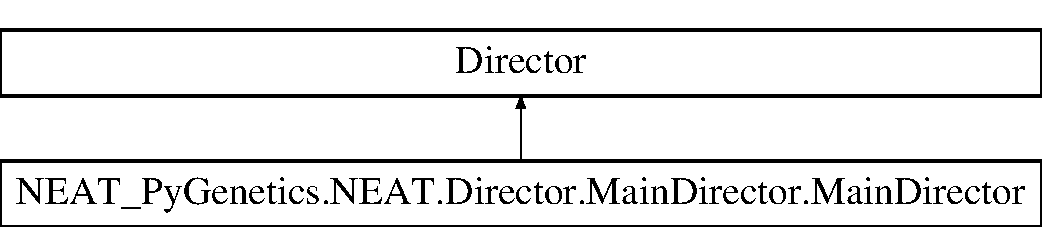
\includegraphics[height=2.000000cm]{classNEAT__PyGenetics_1_1NEAT_1_1Director_1_1MainDirector_1_1MainDirector}
\end{center}
\end{figure}
\subsection*{Public Member Functions}
\begin{DoxyCompactItemize}
\item 
def \hyperlink{classNEAT__PyGenetics_1_1NEAT_1_1Director_1_1MainDirector_1_1MainDirector_ab14b0501fc1b74c88b2e57f2c427f556}{\+\_\+\+\_\+init\+\_\+\+\_\+} (self, kwargs)
\begin{DoxyCompactList}\small\item\em \+:param kwargs\+: \end{DoxyCompactList}\item 
def \hyperlink{classNEAT__PyGenetics_1_1NEAT_1_1Director_1_1MainDirector_1_1MainDirector_ae092b13a0703771ac0813e67fb872362}{idle} (self)
\begin{DoxyCompactList}\small\item\em Standard method that will be executed if local startup is done. \end{DoxyCompactList}\item 
def \hyperlink{classNEAT__PyGenetics_1_1NEAT_1_1Director_1_1MainDirector_1_1MainDirector_a145a35253c447b14b3a834cd6bbd6b15}{dynamic\+\_\+init} (self)
\begin{DoxyCompactList}\small\item\em Initializes all parts of \hyperlink{namespaceNEAT__PyGenetics_1_1NEAT}{N\+E\+AT} that are dependent upon the client. \end{DoxyCompactList}\item 
def \hyperlink{classNEAT__PyGenetics_1_1NEAT_1_1Director_1_1MainDirector_1_1MainDirector_a1d54dab714e07b9ba097b118994bc7e0}{init\+\_\+db} (self)
\item 
def \hyperlink{classNEAT__PyGenetics_1_1NEAT_1_1Director_1_1MainDirector_1_1MainDirector_a0dc96b0a3075b0522e9179e154e3bfdc}{run} (self)
\begin{DoxyCompactList}\small\item\em The main function where the simulation is run, new genomes are created and discarded This is where the evolutionary magic happens. \end{DoxyCompactList}\item 
def \hyperlink{classNEAT__PyGenetics_1_1NEAT_1_1Director_1_1MainDirector_1_1MainDirector_a62d21475b9a55ebf26b731e1af031998}{generate\+\_\+new\+\_\+genomes} (self)
\begin{DoxyCompactList}\small\item\em Regenerates the population by selecting genomes for mutation / breeding, running the generation process and performing analysis. \end{DoxyCompactList}\item 
def \hyperlink{classNEAT__PyGenetics_1_1NEAT_1_1Director_1_1MainDirector_1_1MainDirector_a24b32672d44473d0ed697d72326a3ed0}{crossbreed\+\_\+clusters} (self)
\begin{DoxyCompactList}\small\item\em combines two clusters by breeding genomes of both clusters \+:return\+: \end{DoxyCompactList}\item 
def \hyperlink{classNEAT__PyGenetics_1_1NEAT_1_1Director_1_1MainDirector_1_1MainDirector_af9ec8145b3a3dc21f823d38b3ea08df1}{analyze\+\_\+and\+\_\+insert}
\item 
def \hyperlink{classNEAT__PyGenetics_1_1NEAT_1_1Director_1_1MainDirector_1_1MainDirector_afc0fd1df30dc28284a1c9552b507298e}{calculate\+\_\+cluster\+\_\+offspring} (self)
\begin{DoxyCompactList}\small\item\em Calculates fitness values and offspring for clusters. \end{DoxyCompactList}\item 
def \hyperlink{classNEAT__PyGenetics_1_1NEAT_1_1Director_1_1MainDirector_1_1MainDirector_a477d29aba8bdf6743748389dce049b9a}{discard\+\_\+genomes} (self)
\begin{DoxyCompactList}\small\item\em discards a number of genomes \+:return\+: \end{DoxyCompactList}\item 
def \hyperlink{classNEAT__PyGenetics_1_1NEAT_1_1Director_1_1MainDirector_1_1MainDirector_a2916d65736e93f21a9a2a8f31d234615}{discard\+\_\+clusters} (self)
\begin{DoxyCompactList}\small\item\em Discards a number of clusters \+:return\+: \end{DoxyCompactList}\item 
def \hyperlink{classNEAT__PyGenetics_1_1NEAT_1_1Director_1_1MainDirector_1_1MainDirector_a233974c8f6d855886617f80737fb44eb}{perform\+\_\+simulation\+\_\+io} (self)
\item 
def \hyperlink{classNEAT__PyGenetics_1_1NEAT_1_1Director_1_1MainDirector_1_1MainDirector_a37de122cc8ac060871f2af4da1a0a1c1}{compute\+\_\+genome\+\_\+outputs}
\item 
def \hyperlink{classNEAT__PyGenetics_1_1NEAT_1_1Director_1_1MainDirector_1_1MainDirector_ab2602e228a2b8c979d4634ec21b542a8}{update\+\_\+fitness\+\_\+values}
\item 
def \hyperlink{classNEAT__PyGenetics_1_1NEAT_1_1Director_1_1MainDirector_1_1MainDirector_af3c8f23fba40f82bfa1a7d0b504bb218}{init\+\_\+population} (self)
\end{DoxyCompactItemize}
\subsection*{Public Attributes}
\begin{DoxyCompactItemize}
\item 
\hyperlink{classNEAT__PyGenetics_1_1NEAT_1_1Director_1_1MainDirector_1_1MainDirector_aefb726fd87bcf69dcdfe897821481894}{mode}
\item 
\hyperlink{classNEAT__PyGenetics_1_1NEAT_1_1Director_1_1MainDirector_1_1MainDirector_a81175102b01b335eae3667ac36c9701f}{selector}
\item 
\hyperlink{classNEAT__PyGenetics_1_1NEAT_1_1Director_1_1MainDirector_1_1MainDirector_accfcd32564920c4fd44a90d07e25e5c1}{decision\+\_\+maker}
\item 
\hyperlink{classNEAT__PyGenetics_1_1NEAT_1_1Director_1_1MainDirector_1_1MainDirector_ad5b0e831f4fbc69f41056db9e477846f}{breeder}
\item 
\hyperlink{classNEAT__PyGenetics_1_1NEAT_1_1Director_1_1MainDirector_1_1MainDirector_a46ea344b5ebeead2d2d29d22ac0d3bdc}{mutator}
\item 
\hyperlink{classNEAT__PyGenetics_1_1NEAT_1_1Director_1_1MainDirector_1_1MainDirector_a2a74e9a3bfe1ee80dd5a14301d05999b}{analyst}
\item 
\hyperlink{classNEAT__PyGenetics_1_1NEAT_1_1Director_1_1MainDirector_1_1MainDirector_a9a61632f5cc72eda0e565dec59ec4956}{clusterer}
\item 
\hyperlink{classNEAT__PyGenetics_1_1NEAT_1_1Director_1_1MainDirector_1_1MainDirector_a7888676faa8495bfe14559664627736d}{simulator}
\item 
\hyperlink{classNEAT__PyGenetics_1_1NEAT_1_1Director_1_1MainDirector_1_1MainDirector_ab2c51deb9fa883d19a1e7c5580e60aaf}{simulation\+\_\+connector}
\item 
\hyperlink{classNEAT__PyGenetics_1_1NEAT_1_1Director_1_1MainDirector_1_1MainDirector_a436be8b6a5893f8ade9d83a812892c35}{database\+\_\+connector}
\item 
\hyperlink{classNEAT__PyGenetics_1_1NEAT_1_1Director_1_1MainDirector_1_1MainDirector_a31df2d6f00d083b4685216a235a87ebc}{gene\+\_\+repository}
\item 
\hyperlink{classNEAT__PyGenetics_1_1NEAT_1_1Director_1_1MainDirector_1_1MainDirector_a144b9b844aa917302a73065d35a9291e}{genome\+\_\+repository}
\item 
\hyperlink{classNEAT__PyGenetics_1_1NEAT_1_1Director_1_1MainDirector_1_1MainDirector_a96c18a6a555495afe445aadddbdcfa6f}{cluster\+\_\+repository}
\item 
\hyperlink{classNEAT__PyGenetics_1_1NEAT_1_1Director_1_1MainDirector_1_1MainDirector_a510d20e601183c53383179cf827ef7af}{config}
\end{DoxyCompactItemize}
\subsection*{Static Public Attributes}
\begin{DoxyCompactItemize}
\item 
\hyperlink{classNEAT__PyGenetics_1_1NEAT_1_1Director_1_1MainDirector_1_1MainDirector_acd18b971efa2d58d414e1aedcafb065d}{results}
\item 
\hyperlink{classNEAT__PyGenetics_1_1NEAT_1_1Director_1_1MainDirector_1_1MainDirector_ac579f78b49d7a2711bf925459dd1266d}{storage\+\_\+genome}
\item 
\hyperlink{classNEAT__PyGenetics_1_1NEAT_1_1Director_1_1MainDirector_1_1MainDirector_ab3116c3ed89cc021eb261dc9f3913cd2}{outputs}
\end{DoxyCompactItemize}


\subsection{Constructor \& Destructor Documentation}
\index{N\+E\+A\+T\+\_\+\+Py\+Genetics\+::\+N\+E\+A\+T\+::\+Director\+::\+Main\+Director\+::\+Main\+Director@{N\+E\+A\+T\+\_\+\+Py\+Genetics\+::\+N\+E\+A\+T\+::\+Director\+::\+Main\+Director\+::\+Main\+Director}!\+\_\+\+\_\+init\+\_\+\+\_\+@{\+\_\+\+\_\+init\+\_\+\+\_\+}}
\index{\+\_\+\+\_\+init\+\_\+\+\_\+@{\+\_\+\+\_\+init\+\_\+\+\_\+}!N\+E\+A\+T\+\_\+\+Py\+Genetics\+::\+N\+E\+A\+T\+::\+Director\+::\+Main\+Director\+::\+Main\+Director@{N\+E\+A\+T\+\_\+\+Py\+Genetics\+::\+N\+E\+A\+T\+::\+Director\+::\+Main\+Director\+::\+Main\+Director}}
\subsubsection[{\texorpdfstring{\+\_\+\+\_\+init\+\_\+\+\_\+(self, kwargs)}{__init__(self, kwargs)}}]{\setlength{\rightskip}{0pt plus 5cm}def N\+E\+A\+T\+\_\+\+Py\+Genetics.\+N\+E\+A\+T.\+Director.\+Main\+Director.\+Main\+Director.\+\_\+\+\_\+init\+\_\+\+\_\+ (
\begin{DoxyParamCaption}
\item[{}]{self, }
\item[{}]{kwargs}
\end{DoxyParamCaption}
)}\hypertarget{classNEAT__PyGenetics_1_1NEAT_1_1Director_1_1MainDirector_1_1MainDirector_ab14b0501fc1b74c88b2e57f2c427f556}{}\label{classNEAT__PyGenetics_1_1NEAT_1_1Director_1_1MainDirector_1_1MainDirector_ab14b0501fc1b74c88b2e57f2c427f556}


\+:param kwargs\+: 


\begin{DoxyItemize}
\item mode\+:
\begin{DoxyItemize}
\item exit\+: exits the program, default action if nothing is provided.
\item new\+: creates a new database for a given simulation. requires parame-\/ ter simulation to be set.
\item load\+: loads a database for a given simulation. requires parameter simulation to be set.
\end{DoxyItemize}
\item simulation\+: the name of the simulation that should be used. must cor-\/ respond to a module name in Simulation. \+:return\+: 
\end{DoxyItemize}

\subsection{Member Function Documentation}
\index{N\+E\+A\+T\+\_\+\+Py\+Genetics\+::\+N\+E\+A\+T\+::\+Director\+::\+Main\+Director\+::\+Main\+Director@{N\+E\+A\+T\+\_\+\+Py\+Genetics\+::\+N\+E\+A\+T\+::\+Director\+::\+Main\+Director\+::\+Main\+Director}!analyze\+\_\+and\+\_\+insert@{analyze\+\_\+and\+\_\+insert}}
\index{analyze\+\_\+and\+\_\+insert@{analyze\+\_\+and\+\_\+insert}!N\+E\+A\+T\+\_\+\+Py\+Genetics\+::\+N\+E\+A\+T\+::\+Director\+::\+Main\+Director\+::\+Main\+Director@{N\+E\+A\+T\+\_\+\+Py\+Genetics\+::\+N\+E\+A\+T\+::\+Director\+::\+Main\+Director\+::\+Main\+Director}}
\subsubsection[{\texorpdfstring{analyze\+\_\+and\+\_\+insert}{analyze_and_insert}}]{\setlength{\rightskip}{0pt plus 5cm}def N\+E\+A\+T\+\_\+\+Py\+Genetics.\+N\+E\+A\+T.\+Director.\+Main\+Director.\+Main\+Director.\+analyze\+\_\+and\+\_\+insert (
\begin{DoxyParamCaption}
\item[{}]{self, }
\item[{}]{genome}
\end{DoxyParamCaption}
)}\hypertarget{classNEAT__PyGenetics_1_1NEAT_1_1Director_1_1MainDirector_1_1MainDirector_af9ec8145b3a3dc21f823d38b3ea08df1}{}\label{classNEAT__PyGenetics_1_1NEAT_1_1Director_1_1MainDirector_1_1MainDirector_af9ec8145b3a3dc21f823d38b3ea08df1}
\index{N\+E\+A\+T\+\_\+\+Py\+Genetics\+::\+N\+E\+A\+T\+::\+Director\+::\+Main\+Director\+::\+Main\+Director@{N\+E\+A\+T\+\_\+\+Py\+Genetics\+::\+N\+E\+A\+T\+::\+Director\+::\+Main\+Director\+::\+Main\+Director}!calculate\+\_\+cluster\+\_\+offspring@{calculate\+\_\+cluster\+\_\+offspring}}
\index{calculate\+\_\+cluster\+\_\+offspring@{calculate\+\_\+cluster\+\_\+offspring}!N\+E\+A\+T\+\_\+\+Py\+Genetics\+::\+N\+E\+A\+T\+::\+Director\+::\+Main\+Director\+::\+Main\+Director@{N\+E\+A\+T\+\_\+\+Py\+Genetics\+::\+N\+E\+A\+T\+::\+Director\+::\+Main\+Director\+::\+Main\+Director}}
\subsubsection[{\texorpdfstring{calculate\+\_\+cluster\+\_\+offspring(self)}{calculate_cluster_offspring(self)}}]{\setlength{\rightskip}{0pt plus 5cm}def N\+E\+A\+T\+\_\+\+Py\+Genetics.\+N\+E\+A\+T.\+Director.\+Main\+Director.\+Main\+Director.\+calculate\+\_\+cluster\+\_\+offspring (
\begin{DoxyParamCaption}
\item[{}]{self}
\end{DoxyParamCaption}
)}\hypertarget{classNEAT__PyGenetics_1_1NEAT_1_1Director_1_1MainDirector_1_1MainDirector_afc0fd1df30dc28284a1c9552b507298e}{}\label{classNEAT__PyGenetics_1_1NEAT_1_1Director_1_1MainDirector_1_1MainDirector_afc0fd1df30dc28284a1c9552b507298e}


Calculates fitness values and offspring for clusters. 

\+:return\+: \index{N\+E\+A\+T\+\_\+\+Py\+Genetics\+::\+N\+E\+A\+T\+::\+Director\+::\+Main\+Director\+::\+Main\+Director@{N\+E\+A\+T\+\_\+\+Py\+Genetics\+::\+N\+E\+A\+T\+::\+Director\+::\+Main\+Director\+::\+Main\+Director}!compute\+\_\+genome\+\_\+outputs@{compute\+\_\+genome\+\_\+outputs}}
\index{compute\+\_\+genome\+\_\+outputs@{compute\+\_\+genome\+\_\+outputs}!N\+E\+A\+T\+\_\+\+Py\+Genetics\+::\+N\+E\+A\+T\+::\+Director\+::\+Main\+Director\+::\+Main\+Director@{N\+E\+A\+T\+\_\+\+Py\+Genetics\+::\+N\+E\+A\+T\+::\+Director\+::\+Main\+Director\+::\+Main\+Director}}
\subsubsection[{\texorpdfstring{compute\+\_\+genome\+\_\+outputs}{compute_genome_outputs}}]{\setlength{\rightskip}{0pt plus 5cm}def N\+E\+A\+T\+\_\+\+Py\+Genetics.\+N\+E\+A\+T.\+Director.\+Main\+Director.\+Main\+Director.\+compute\+\_\+genome\+\_\+outputs (
\begin{DoxyParamCaption}
\item[{}]{self, }
\item[{}]{block\+\_\+inputs}
\end{DoxyParamCaption}
)}\hypertarget{classNEAT__PyGenetics_1_1NEAT_1_1Director_1_1MainDirector_1_1MainDirector_a37de122cc8ac060871f2af4da1a0a1c1}{}\label{classNEAT__PyGenetics_1_1NEAT_1_1Director_1_1MainDirector_1_1MainDirector_a37de122cc8ac060871f2af4da1a0a1c1}
\index{N\+E\+A\+T\+\_\+\+Py\+Genetics\+::\+N\+E\+A\+T\+::\+Director\+::\+Main\+Director\+::\+Main\+Director@{N\+E\+A\+T\+\_\+\+Py\+Genetics\+::\+N\+E\+A\+T\+::\+Director\+::\+Main\+Director\+::\+Main\+Director}!crossbreed\+\_\+clusters@{crossbreed\+\_\+clusters}}
\index{crossbreed\+\_\+clusters@{crossbreed\+\_\+clusters}!N\+E\+A\+T\+\_\+\+Py\+Genetics\+::\+N\+E\+A\+T\+::\+Director\+::\+Main\+Director\+::\+Main\+Director@{N\+E\+A\+T\+\_\+\+Py\+Genetics\+::\+N\+E\+A\+T\+::\+Director\+::\+Main\+Director\+::\+Main\+Director}}
\subsubsection[{\texorpdfstring{crossbreed\+\_\+clusters(self)}{crossbreed_clusters(self)}}]{\setlength{\rightskip}{0pt plus 5cm}def N\+E\+A\+T\+\_\+\+Py\+Genetics.\+N\+E\+A\+T.\+Director.\+Main\+Director.\+Main\+Director.\+crossbreed\+\_\+clusters (
\begin{DoxyParamCaption}
\item[{}]{self}
\end{DoxyParamCaption}
)}\hypertarget{classNEAT__PyGenetics_1_1NEAT_1_1Director_1_1MainDirector_1_1MainDirector_a24b32672d44473d0ed697d72326a3ed0}{}\label{classNEAT__PyGenetics_1_1NEAT_1_1Director_1_1MainDirector_1_1MainDirector_a24b32672d44473d0ed697d72326a3ed0}


combines two clusters by breeding genomes of both clusters \+:return\+: 

\index{N\+E\+A\+T\+\_\+\+Py\+Genetics\+::\+N\+E\+A\+T\+::\+Director\+::\+Main\+Director\+::\+Main\+Director@{N\+E\+A\+T\+\_\+\+Py\+Genetics\+::\+N\+E\+A\+T\+::\+Director\+::\+Main\+Director\+::\+Main\+Director}!discard\+\_\+clusters@{discard\+\_\+clusters}}
\index{discard\+\_\+clusters@{discard\+\_\+clusters}!N\+E\+A\+T\+\_\+\+Py\+Genetics\+::\+N\+E\+A\+T\+::\+Director\+::\+Main\+Director\+::\+Main\+Director@{N\+E\+A\+T\+\_\+\+Py\+Genetics\+::\+N\+E\+A\+T\+::\+Director\+::\+Main\+Director\+::\+Main\+Director}}
\subsubsection[{\texorpdfstring{discard\+\_\+clusters(self)}{discard_clusters(self)}}]{\setlength{\rightskip}{0pt plus 5cm}def N\+E\+A\+T\+\_\+\+Py\+Genetics.\+N\+E\+A\+T.\+Director.\+Main\+Director.\+Main\+Director.\+discard\+\_\+clusters (
\begin{DoxyParamCaption}
\item[{}]{self}
\end{DoxyParamCaption}
)}\hypertarget{classNEAT__PyGenetics_1_1NEAT_1_1Director_1_1MainDirector_1_1MainDirector_a2916d65736e93f21a9a2a8f31d234615}{}\label{classNEAT__PyGenetics_1_1NEAT_1_1Director_1_1MainDirector_1_1MainDirector_a2916d65736e93f21a9a2a8f31d234615}


Discards a number of clusters \+:return\+: 

\index{N\+E\+A\+T\+\_\+\+Py\+Genetics\+::\+N\+E\+A\+T\+::\+Director\+::\+Main\+Director\+::\+Main\+Director@{N\+E\+A\+T\+\_\+\+Py\+Genetics\+::\+N\+E\+A\+T\+::\+Director\+::\+Main\+Director\+::\+Main\+Director}!discard\+\_\+genomes@{discard\+\_\+genomes}}
\index{discard\+\_\+genomes@{discard\+\_\+genomes}!N\+E\+A\+T\+\_\+\+Py\+Genetics\+::\+N\+E\+A\+T\+::\+Director\+::\+Main\+Director\+::\+Main\+Director@{N\+E\+A\+T\+\_\+\+Py\+Genetics\+::\+N\+E\+A\+T\+::\+Director\+::\+Main\+Director\+::\+Main\+Director}}
\subsubsection[{\texorpdfstring{discard\+\_\+genomes(self)}{discard_genomes(self)}}]{\setlength{\rightskip}{0pt plus 5cm}def N\+E\+A\+T\+\_\+\+Py\+Genetics.\+N\+E\+A\+T.\+Director.\+Main\+Director.\+Main\+Director.\+discard\+\_\+genomes (
\begin{DoxyParamCaption}
\item[{}]{self}
\end{DoxyParamCaption}
)}\hypertarget{classNEAT__PyGenetics_1_1NEAT_1_1Director_1_1MainDirector_1_1MainDirector_a477d29aba8bdf6743748389dce049b9a}{}\label{classNEAT__PyGenetics_1_1NEAT_1_1Director_1_1MainDirector_1_1MainDirector_a477d29aba8bdf6743748389dce049b9a}


discards a number of genomes \+:return\+: 

\index{N\+E\+A\+T\+\_\+\+Py\+Genetics\+::\+N\+E\+A\+T\+::\+Director\+::\+Main\+Director\+::\+Main\+Director@{N\+E\+A\+T\+\_\+\+Py\+Genetics\+::\+N\+E\+A\+T\+::\+Director\+::\+Main\+Director\+::\+Main\+Director}!dynamic\+\_\+init@{dynamic\+\_\+init}}
\index{dynamic\+\_\+init@{dynamic\+\_\+init}!N\+E\+A\+T\+\_\+\+Py\+Genetics\+::\+N\+E\+A\+T\+::\+Director\+::\+Main\+Director\+::\+Main\+Director@{N\+E\+A\+T\+\_\+\+Py\+Genetics\+::\+N\+E\+A\+T\+::\+Director\+::\+Main\+Director\+::\+Main\+Director}}
\subsubsection[{\texorpdfstring{dynamic\+\_\+init(self)}{dynamic_init(self)}}]{\setlength{\rightskip}{0pt plus 5cm}def N\+E\+A\+T\+\_\+\+Py\+Genetics.\+N\+E\+A\+T.\+Director.\+Main\+Director.\+Main\+Director.\+dynamic\+\_\+init (
\begin{DoxyParamCaption}
\item[{}]{self}
\end{DoxyParamCaption}
)}\hypertarget{classNEAT__PyGenetics_1_1NEAT_1_1Director_1_1MainDirector_1_1MainDirector_a145a35253c447b14b3a834cd6bbd6b15}{}\label{classNEAT__PyGenetics_1_1NEAT_1_1Director_1_1MainDirector_1_1MainDirector_a145a35253c447b14b3a834cd6bbd6b15}


Initializes all parts of \hyperlink{namespaceNEAT__PyGenetics_1_1NEAT}{N\+E\+AT} that are dependent upon the client. 

\index{N\+E\+A\+T\+\_\+\+Py\+Genetics\+::\+N\+E\+A\+T\+::\+Director\+::\+Main\+Director\+::\+Main\+Director@{N\+E\+A\+T\+\_\+\+Py\+Genetics\+::\+N\+E\+A\+T\+::\+Director\+::\+Main\+Director\+::\+Main\+Director}!generate\+\_\+new\+\_\+genomes@{generate\+\_\+new\+\_\+genomes}}
\index{generate\+\_\+new\+\_\+genomes@{generate\+\_\+new\+\_\+genomes}!N\+E\+A\+T\+\_\+\+Py\+Genetics\+::\+N\+E\+A\+T\+::\+Director\+::\+Main\+Director\+::\+Main\+Director@{N\+E\+A\+T\+\_\+\+Py\+Genetics\+::\+N\+E\+A\+T\+::\+Director\+::\+Main\+Director\+::\+Main\+Director}}
\subsubsection[{\texorpdfstring{generate\+\_\+new\+\_\+genomes(self)}{generate_new_genomes(self)}}]{\setlength{\rightskip}{0pt plus 5cm}def N\+E\+A\+T\+\_\+\+Py\+Genetics.\+N\+E\+A\+T.\+Director.\+Main\+Director.\+Main\+Director.\+generate\+\_\+new\+\_\+genomes (
\begin{DoxyParamCaption}
\item[{}]{self}
\end{DoxyParamCaption}
)}\hypertarget{classNEAT__PyGenetics_1_1NEAT_1_1Director_1_1MainDirector_1_1MainDirector_a62d21475b9a55ebf26b731e1af031998}{}\label{classNEAT__PyGenetics_1_1NEAT_1_1Director_1_1MainDirector_1_1MainDirector_a62d21475b9a55ebf26b731e1af031998}


Regenerates the population by selecting genomes for mutation / breeding, running the generation process and performing analysis. 

\+:return\+: \index{N\+E\+A\+T\+\_\+\+Py\+Genetics\+::\+N\+E\+A\+T\+::\+Director\+::\+Main\+Director\+::\+Main\+Director@{N\+E\+A\+T\+\_\+\+Py\+Genetics\+::\+N\+E\+A\+T\+::\+Director\+::\+Main\+Director\+::\+Main\+Director}!idle@{idle}}
\index{idle@{idle}!N\+E\+A\+T\+\_\+\+Py\+Genetics\+::\+N\+E\+A\+T\+::\+Director\+::\+Main\+Director\+::\+Main\+Director@{N\+E\+A\+T\+\_\+\+Py\+Genetics\+::\+N\+E\+A\+T\+::\+Director\+::\+Main\+Director\+::\+Main\+Director}}
\subsubsection[{\texorpdfstring{idle(self)}{idle(self)}}]{\setlength{\rightskip}{0pt plus 5cm}def N\+E\+A\+T\+\_\+\+Py\+Genetics.\+N\+E\+A\+T.\+Director.\+Main\+Director.\+Main\+Director.\+idle (
\begin{DoxyParamCaption}
\item[{}]{self}
\end{DoxyParamCaption}
)}\hypertarget{classNEAT__PyGenetics_1_1NEAT_1_1Director_1_1MainDirector_1_1MainDirector_ae092b13a0703771ac0813e67fb872362}{}\label{classNEAT__PyGenetics_1_1NEAT_1_1Director_1_1MainDirector_1_1MainDirector_ae092b13a0703771ac0813e67fb872362}


Standard method that will be executed if local startup is done. 

In this state, the \hyperlink{namespaceNEAT__PyGenetics_1_1NEAT_1_1Director_1_1Director}{Director} will wait for the client. \index{N\+E\+A\+T\+\_\+\+Py\+Genetics\+::\+N\+E\+A\+T\+::\+Director\+::\+Main\+Director\+::\+Main\+Director@{N\+E\+A\+T\+\_\+\+Py\+Genetics\+::\+N\+E\+A\+T\+::\+Director\+::\+Main\+Director\+::\+Main\+Director}!init\+\_\+db@{init\+\_\+db}}
\index{init\+\_\+db@{init\+\_\+db}!N\+E\+A\+T\+\_\+\+Py\+Genetics\+::\+N\+E\+A\+T\+::\+Director\+::\+Main\+Director\+::\+Main\+Director@{N\+E\+A\+T\+\_\+\+Py\+Genetics\+::\+N\+E\+A\+T\+::\+Director\+::\+Main\+Director\+::\+Main\+Director}}
\subsubsection[{\texorpdfstring{init\+\_\+db(self)}{init_db(self)}}]{\setlength{\rightskip}{0pt plus 5cm}def N\+E\+A\+T\+\_\+\+Py\+Genetics.\+N\+E\+A\+T.\+Director.\+Main\+Director.\+Main\+Director.\+init\+\_\+db (
\begin{DoxyParamCaption}
\item[{}]{self}
\end{DoxyParamCaption}
)}\hypertarget{classNEAT__PyGenetics_1_1NEAT_1_1Director_1_1MainDirector_1_1MainDirector_a1d54dab714e07b9ba097b118994bc7e0}{}\label{classNEAT__PyGenetics_1_1NEAT_1_1Director_1_1MainDirector_1_1MainDirector_a1d54dab714e07b9ba097b118994bc7e0}
\index{N\+E\+A\+T\+\_\+\+Py\+Genetics\+::\+N\+E\+A\+T\+::\+Director\+::\+Main\+Director\+::\+Main\+Director@{N\+E\+A\+T\+\_\+\+Py\+Genetics\+::\+N\+E\+A\+T\+::\+Director\+::\+Main\+Director\+::\+Main\+Director}!init\+\_\+population@{init\+\_\+population}}
\index{init\+\_\+population@{init\+\_\+population}!N\+E\+A\+T\+\_\+\+Py\+Genetics\+::\+N\+E\+A\+T\+::\+Director\+::\+Main\+Director\+::\+Main\+Director@{N\+E\+A\+T\+\_\+\+Py\+Genetics\+::\+N\+E\+A\+T\+::\+Director\+::\+Main\+Director\+::\+Main\+Director}}
\subsubsection[{\texorpdfstring{init\+\_\+population(self)}{init_population(self)}}]{\setlength{\rightskip}{0pt plus 5cm}def N\+E\+A\+T\+\_\+\+Py\+Genetics.\+N\+E\+A\+T.\+Director.\+Main\+Director.\+Main\+Director.\+init\+\_\+population (
\begin{DoxyParamCaption}
\item[{}]{self}
\end{DoxyParamCaption}
)}\hypertarget{classNEAT__PyGenetics_1_1NEAT_1_1Director_1_1MainDirector_1_1MainDirector_af3c8f23fba40f82bfa1a7d0b504bb218}{}\label{classNEAT__PyGenetics_1_1NEAT_1_1Director_1_1MainDirector_1_1MainDirector_af3c8f23fba40f82bfa1a7d0b504bb218}
\index{N\+E\+A\+T\+\_\+\+Py\+Genetics\+::\+N\+E\+A\+T\+::\+Director\+::\+Main\+Director\+::\+Main\+Director@{N\+E\+A\+T\+\_\+\+Py\+Genetics\+::\+N\+E\+A\+T\+::\+Director\+::\+Main\+Director\+::\+Main\+Director}!perform\+\_\+simulation\+\_\+io@{perform\+\_\+simulation\+\_\+io}}
\index{perform\+\_\+simulation\+\_\+io@{perform\+\_\+simulation\+\_\+io}!N\+E\+A\+T\+\_\+\+Py\+Genetics\+::\+N\+E\+A\+T\+::\+Director\+::\+Main\+Director\+::\+Main\+Director@{N\+E\+A\+T\+\_\+\+Py\+Genetics\+::\+N\+E\+A\+T\+::\+Director\+::\+Main\+Director\+::\+Main\+Director}}
\subsubsection[{\texorpdfstring{perform\+\_\+simulation\+\_\+io(self)}{perform_simulation_io(self)}}]{\setlength{\rightskip}{0pt plus 5cm}def N\+E\+A\+T\+\_\+\+Py\+Genetics.\+N\+E\+A\+T.\+Director.\+Main\+Director.\+Main\+Director.\+perform\+\_\+simulation\+\_\+io (
\begin{DoxyParamCaption}
\item[{}]{self}
\end{DoxyParamCaption}
)}\hypertarget{classNEAT__PyGenetics_1_1NEAT_1_1Director_1_1MainDirector_1_1MainDirector_a233974c8f6d855886617f80737fb44eb}{}\label{classNEAT__PyGenetics_1_1NEAT_1_1Director_1_1MainDirector_1_1MainDirector_a233974c8f6d855886617f80737fb44eb}
\index{N\+E\+A\+T\+\_\+\+Py\+Genetics\+::\+N\+E\+A\+T\+::\+Director\+::\+Main\+Director\+::\+Main\+Director@{N\+E\+A\+T\+\_\+\+Py\+Genetics\+::\+N\+E\+A\+T\+::\+Director\+::\+Main\+Director\+::\+Main\+Director}!run@{run}}
\index{run@{run}!N\+E\+A\+T\+\_\+\+Py\+Genetics\+::\+N\+E\+A\+T\+::\+Director\+::\+Main\+Director\+::\+Main\+Director@{N\+E\+A\+T\+\_\+\+Py\+Genetics\+::\+N\+E\+A\+T\+::\+Director\+::\+Main\+Director\+::\+Main\+Director}}
\subsubsection[{\texorpdfstring{run(self)}{run(self)}}]{\setlength{\rightskip}{0pt plus 5cm}def N\+E\+A\+T\+\_\+\+Py\+Genetics.\+N\+E\+A\+T.\+Director.\+Main\+Director.\+Main\+Director.\+run (
\begin{DoxyParamCaption}
\item[{}]{self}
\end{DoxyParamCaption}
)}\hypertarget{classNEAT__PyGenetics_1_1NEAT_1_1Director_1_1MainDirector_1_1MainDirector_a0dc96b0a3075b0522e9179e154e3bfdc}{}\label{classNEAT__PyGenetics_1_1NEAT_1_1Director_1_1MainDirector_1_1MainDirector_a0dc96b0a3075b0522e9179e154e3bfdc}


The main function where the simulation is run, new genomes are created and discarded This is where the evolutionary magic happens. 

\index{N\+E\+A\+T\+\_\+\+Py\+Genetics\+::\+N\+E\+A\+T\+::\+Director\+::\+Main\+Director\+::\+Main\+Director@{N\+E\+A\+T\+\_\+\+Py\+Genetics\+::\+N\+E\+A\+T\+::\+Director\+::\+Main\+Director\+::\+Main\+Director}!update\+\_\+fitness\+\_\+values@{update\+\_\+fitness\+\_\+values}}
\index{update\+\_\+fitness\+\_\+values@{update\+\_\+fitness\+\_\+values}!N\+E\+A\+T\+\_\+\+Py\+Genetics\+::\+N\+E\+A\+T\+::\+Director\+::\+Main\+Director\+::\+Main\+Director@{N\+E\+A\+T\+\_\+\+Py\+Genetics\+::\+N\+E\+A\+T\+::\+Director\+::\+Main\+Director\+::\+Main\+Director}}
\subsubsection[{\texorpdfstring{update\+\_\+fitness\+\_\+values}{update_fitness_values}}]{\setlength{\rightskip}{0pt plus 5cm}def N\+E\+A\+T\+\_\+\+Py\+Genetics.\+N\+E\+A\+T.\+Director.\+Main\+Director.\+Main\+Director.\+update\+\_\+fitness\+\_\+values (
\begin{DoxyParamCaption}
\item[{}]{self, }
\item[{}]{fitness\+\_\+values}
\end{DoxyParamCaption}
)}\hypertarget{classNEAT__PyGenetics_1_1NEAT_1_1Director_1_1MainDirector_1_1MainDirector_ab2602e228a2b8c979d4634ec21b542a8}{}\label{classNEAT__PyGenetics_1_1NEAT_1_1Director_1_1MainDirector_1_1MainDirector_ab2602e228a2b8c979d4634ec21b542a8}


\subsection{Member Data Documentation}
\index{N\+E\+A\+T\+\_\+\+Py\+Genetics\+::\+N\+E\+A\+T\+::\+Director\+::\+Main\+Director\+::\+Main\+Director@{N\+E\+A\+T\+\_\+\+Py\+Genetics\+::\+N\+E\+A\+T\+::\+Director\+::\+Main\+Director\+::\+Main\+Director}!analyst@{analyst}}
\index{analyst@{analyst}!N\+E\+A\+T\+\_\+\+Py\+Genetics\+::\+N\+E\+A\+T\+::\+Director\+::\+Main\+Director\+::\+Main\+Director@{N\+E\+A\+T\+\_\+\+Py\+Genetics\+::\+N\+E\+A\+T\+::\+Director\+::\+Main\+Director\+::\+Main\+Director}}
\subsubsection[{\texorpdfstring{analyst}{analyst}}]{\setlength{\rightskip}{0pt plus 5cm}N\+E\+A\+T\+\_\+\+Py\+Genetics.\+N\+E\+A\+T.\+Director.\+Main\+Director.\+Main\+Director.\+analyst}\hypertarget{classNEAT__PyGenetics_1_1NEAT_1_1Director_1_1MainDirector_1_1MainDirector_a2a74e9a3bfe1ee80dd5a14301d05999b}{}\label{classNEAT__PyGenetics_1_1NEAT_1_1Director_1_1MainDirector_1_1MainDirector_a2a74e9a3bfe1ee80dd5a14301d05999b}
\index{N\+E\+A\+T\+\_\+\+Py\+Genetics\+::\+N\+E\+A\+T\+::\+Director\+::\+Main\+Director\+::\+Main\+Director@{N\+E\+A\+T\+\_\+\+Py\+Genetics\+::\+N\+E\+A\+T\+::\+Director\+::\+Main\+Director\+::\+Main\+Director}!breeder@{breeder}}
\index{breeder@{breeder}!N\+E\+A\+T\+\_\+\+Py\+Genetics\+::\+N\+E\+A\+T\+::\+Director\+::\+Main\+Director\+::\+Main\+Director@{N\+E\+A\+T\+\_\+\+Py\+Genetics\+::\+N\+E\+A\+T\+::\+Director\+::\+Main\+Director\+::\+Main\+Director}}
\subsubsection[{\texorpdfstring{breeder}{breeder}}]{\setlength{\rightskip}{0pt plus 5cm}N\+E\+A\+T\+\_\+\+Py\+Genetics.\+N\+E\+A\+T.\+Director.\+Main\+Director.\+Main\+Director.\+breeder}\hypertarget{classNEAT__PyGenetics_1_1NEAT_1_1Director_1_1MainDirector_1_1MainDirector_ad5b0e831f4fbc69f41056db9e477846f}{}\label{classNEAT__PyGenetics_1_1NEAT_1_1Director_1_1MainDirector_1_1MainDirector_ad5b0e831f4fbc69f41056db9e477846f}
\index{N\+E\+A\+T\+\_\+\+Py\+Genetics\+::\+N\+E\+A\+T\+::\+Director\+::\+Main\+Director\+::\+Main\+Director@{N\+E\+A\+T\+\_\+\+Py\+Genetics\+::\+N\+E\+A\+T\+::\+Director\+::\+Main\+Director\+::\+Main\+Director}!cluster\+\_\+repository@{cluster\+\_\+repository}}
\index{cluster\+\_\+repository@{cluster\+\_\+repository}!N\+E\+A\+T\+\_\+\+Py\+Genetics\+::\+N\+E\+A\+T\+::\+Director\+::\+Main\+Director\+::\+Main\+Director@{N\+E\+A\+T\+\_\+\+Py\+Genetics\+::\+N\+E\+A\+T\+::\+Director\+::\+Main\+Director\+::\+Main\+Director}}
\subsubsection[{\texorpdfstring{cluster\+\_\+repository}{cluster_repository}}]{\setlength{\rightskip}{0pt plus 5cm}N\+E\+A\+T\+\_\+\+Py\+Genetics.\+N\+E\+A\+T.\+Director.\+Main\+Director.\+Main\+Director.\+cluster\+\_\+repository}\hypertarget{classNEAT__PyGenetics_1_1NEAT_1_1Director_1_1MainDirector_1_1MainDirector_a96c18a6a555495afe445aadddbdcfa6f}{}\label{classNEAT__PyGenetics_1_1NEAT_1_1Director_1_1MainDirector_1_1MainDirector_a96c18a6a555495afe445aadddbdcfa6f}
\index{N\+E\+A\+T\+\_\+\+Py\+Genetics\+::\+N\+E\+A\+T\+::\+Director\+::\+Main\+Director\+::\+Main\+Director@{N\+E\+A\+T\+\_\+\+Py\+Genetics\+::\+N\+E\+A\+T\+::\+Director\+::\+Main\+Director\+::\+Main\+Director}!clusterer@{clusterer}}
\index{clusterer@{clusterer}!N\+E\+A\+T\+\_\+\+Py\+Genetics\+::\+N\+E\+A\+T\+::\+Director\+::\+Main\+Director\+::\+Main\+Director@{N\+E\+A\+T\+\_\+\+Py\+Genetics\+::\+N\+E\+A\+T\+::\+Director\+::\+Main\+Director\+::\+Main\+Director}}
\subsubsection[{\texorpdfstring{clusterer}{clusterer}}]{\setlength{\rightskip}{0pt plus 5cm}N\+E\+A\+T\+\_\+\+Py\+Genetics.\+N\+E\+A\+T.\+Director.\+Main\+Director.\+Main\+Director.\+clusterer}\hypertarget{classNEAT__PyGenetics_1_1NEAT_1_1Director_1_1MainDirector_1_1MainDirector_a9a61632f5cc72eda0e565dec59ec4956}{}\label{classNEAT__PyGenetics_1_1NEAT_1_1Director_1_1MainDirector_1_1MainDirector_a9a61632f5cc72eda0e565dec59ec4956}
\index{N\+E\+A\+T\+\_\+\+Py\+Genetics\+::\+N\+E\+A\+T\+::\+Director\+::\+Main\+Director\+::\+Main\+Director@{N\+E\+A\+T\+\_\+\+Py\+Genetics\+::\+N\+E\+A\+T\+::\+Director\+::\+Main\+Director\+::\+Main\+Director}!config@{config}}
\index{config@{config}!N\+E\+A\+T\+\_\+\+Py\+Genetics\+::\+N\+E\+A\+T\+::\+Director\+::\+Main\+Director\+::\+Main\+Director@{N\+E\+A\+T\+\_\+\+Py\+Genetics\+::\+N\+E\+A\+T\+::\+Director\+::\+Main\+Director\+::\+Main\+Director}}
\subsubsection[{\texorpdfstring{config}{config}}]{\setlength{\rightskip}{0pt plus 5cm}N\+E\+A\+T\+\_\+\+Py\+Genetics.\+N\+E\+A\+T.\+Director.\+Main\+Director.\+Main\+Director.\+config}\hypertarget{classNEAT__PyGenetics_1_1NEAT_1_1Director_1_1MainDirector_1_1MainDirector_a510d20e601183c53383179cf827ef7af}{}\label{classNEAT__PyGenetics_1_1NEAT_1_1Director_1_1MainDirector_1_1MainDirector_a510d20e601183c53383179cf827ef7af}
\index{N\+E\+A\+T\+\_\+\+Py\+Genetics\+::\+N\+E\+A\+T\+::\+Director\+::\+Main\+Director\+::\+Main\+Director@{N\+E\+A\+T\+\_\+\+Py\+Genetics\+::\+N\+E\+A\+T\+::\+Director\+::\+Main\+Director\+::\+Main\+Director}!database\+\_\+connector@{database\+\_\+connector}}
\index{database\+\_\+connector@{database\+\_\+connector}!N\+E\+A\+T\+\_\+\+Py\+Genetics\+::\+N\+E\+A\+T\+::\+Director\+::\+Main\+Director\+::\+Main\+Director@{N\+E\+A\+T\+\_\+\+Py\+Genetics\+::\+N\+E\+A\+T\+::\+Director\+::\+Main\+Director\+::\+Main\+Director}}
\subsubsection[{\texorpdfstring{database\+\_\+connector}{database_connector}}]{\setlength{\rightskip}{0pt plus 5cm}N\+E\+A\+T\+\_\+\+Py\+Genetics.\+N\+E\+A\+T.\+Director.\+Main\+Director.\+Main\+Director.\+database\+\_\+connector}\hypertarget{classNEAT__PyGenetics_1_1NEAT_1_1Director_1_1MainDirector_1_1MainDirector_a436be8b6a5893f8ade9d83a812892c35}{}\label{classNEAT__PyGenetics_1_1NEAT_1_1Director_1_1MainDirector_1_1MainDirector_a436be8b6a5893f8ade9d83a812892c35}
\index{N\+E\+A\+T\+\_\+\+Py\+Genetics\+::\+N\+E\+A\+T\+::\+Director\+::\+Main\+Director\+::\+Main\+Director@{N\+E\+A\+T\+\_\+\+Py\+Genetics\+::\+N\+E\+A\+T\+::\+Director\+::\+Main\+Director\+::\+Main\+Director}!decision\+\_\+maker@{decision\+\_\+maker}}
\index{decision\+\_\+maker@{decision\+\_\+maker}!N\+E\+A\+T\+\_\+\+Py\+Genetics\+::\+N\+E\+A\+T\+::\+Director\+::\+Main\+Director\+::\+Main\+Director@{N\+E\+A\+T\+\_\+\+Py\+Genetics\+::\+N\+E\+A\+T\+::\+Director\+::\+Main\+Director\+::\+Main\+Director}}
\subsubsection[{\texorpdfstring{decision\+\_\+maker}{decision_maker}}]{\setlength{\rightskip}{0pt plus 5cm}N\+E\+A\+T\+\_\+\+Py\+Genetics.\+N\+E\+A\+T.\+Director.\+Main\+Director.\+Main\+Director.\+decision\+\_\+maker}\hypertarget{classNEAT__PyGenetics_1_1NEAT_1_1Director_1_1MainDirector_1_1MainDirector_accfcd32564920c4fd44a90d07e25e5c1}{}\label{classNEAT__PyGenetics_1_1NEAT_1_1Director_1_1MainDirector_1_1MainDirector_accfcd32564920c4fd44a90d07e25e5c1}
\index{N\+E\+A\+T\+\_\+\+Py\+Genetics\+::\+N\+E\+A\+T\+::\+Director\+::\+Main\+Director\+::\+Main\+Director@{N\+E\+A\+T\+\_\+\+Py\+Genetics\+::\+N\+E\+A\+T\+::\+Director\+::\+Main\+Director\+::\+Main\+Director}!gene\+\_\+repository@{gene\+\_\+repository}}
\index{gene\+\_\+repository@{gene\+\_\+repository}!N\+E\+A\+T\+\_\+\+Py\+Genetics\+::\+N\+E\+A\+T\+::\+Director\+::\+Main\+Director\+::\+Main\+Director@{N\+E\+A\+T\+\_\+\+Py\+Genetics\+::\+N\+E\+A\+T\+::\+Director\+::\+Main\+Director\+::\+Main\+Director}}
\subsubsection[{\texorpdfstring{gene\+\_\+repository}{gene_repository}}]{\setlength{\rightskip}{0pt plus 5cm}N\+E\+A\+T\+\_\+\+Py\+Genetics.\+N\+E\+A\+T.\+Director.\+Main\+Director.\+Main\+Director.\+gene\+\_\+repository}\hypertarget{classNEAT__PyGenetics_1_1NEAT_1_1Director_1_1MainDirector_1_1MainDirector_a31df2d6f00d083b4685216a235a87ebc}{}\label{classNEAT__PyGenetics_1_1NEAT_1_1Director_1_1MainDirector_1_1MainDirector_a31df2d6f00d083b4685216a235a87ebc}
\index{N\+E\+A\+T\+\_\+\+Py\+Genetics\+::\+N\+E\+A\+T\+::\+Director\+::\+Main\+Director\+::\+Main\+Director@{N\+E\+A\+T\+\_\+\+Py\+Genetics\+::\+N\+E\+A\+T\+::\+Director\+::\+Main\+Director\+::\+Main\+Director}!genome\+\_\+repository@{genome\+\_\+repository}}
\index{genome\+\_\+repository@{genome\+\_\+repository}!N\+E\+A\+T\+\_\+\+Py\+Genetics\+::\+N\+E\+A\+T\+::\+Director\+::\+Main\+Director\+::\+Main\+Director@{N\+E\+A\+T\+\_\+\+Py\+Genetics\+::\+N\+E\+A\+T\+::\+Director\+::\+Main\+Director\+::\+Main\+Director}}
\subsubsection[{\texorpdfstring{genome\+\_\+repository}{genome_repository}}]{\setlength{\rightskip}{0pt plus 5cm}N\+E\+A\+T\+\_\+\+Py\+Genetics.\+N\+E\+A\+T.\+Director.\+Main\+Director.\+Main\+Director.\+genome\+\_\+repository}\hypertarget{classNEAT__PyGenetics_1_1NEAT_1_1Director_1_1MainDirector_1_1MainDirector_a144b9b844aa917302a73065d35a9291e}{}\label{classNEAT__PyGenetics_1_1NEAT_1_1Director_1_1MainDirector_1_1MainDirector_a144b9b844aa917302a73065d35a9291e}
\index{N\+E\+A\+T\+\_\+\+Py\+Genetics\+::\+N\+E\+A\+T\+::\+Director\+::\+Main\+Director\+::\+Main\+Director@{N\+E\+A\+T\+\_\+\+Py\+Genetics\+::\+N\+E\+A\+T\+::\+Director\+::\+Main\+Director\+::\+Main\+Director}!mode@{mode}}
\index{mode@{mode}!N\+E\+A\+T\+\_\+\+Py\+Genetics\+::\+N\+E\+A\+T\+::\+Director\+::\+Main\+Director\+::\+Main\+Director@{N\+E\+A\+T\+\_\+\+Py\+Genetics\+::\+N\+E\+A\+T\+::\+Director\+::\+Main\+Director\+::\+Main\+Director}}
\subsubsection[{\texorpdfstring{mode}{mode}}]{\setlength{\rightskip}{0pt plus 5cm}N\+E\+A\+T\+\_\+\+Py\+Genetics.\+N\+E\+A\+T.\+Director.\+Main\+Director.\+Main\+Director.\+mode}\hypertarget{classNEAT__PyGenetics_1_1NEAT_1_1Director_1_1MainDirector_1_1MainDirector_aefb726fd87bcf69dcdfe897821481894}{}\label{classNEAT__PyGenetics_1_1NEAT_1_1Director_1_1MainDirector_1_1MainDirector_aefb726fd87bcf69dcdfe897821481894}
\index{N\+E\+A\+T\+\_\+\+Py\+Genetics\+::\+N\+E\+A\+T\+::\+Director\+::\+Main\+Director\+::\+Main\+Director@{N\+E\+A\+T\+\_\+\+Py\+Genetics\+::\+N\+E\+A\+T\+::\+Director\+::\+Main\+Director\+::\+Main\+Director}!mutator@{mutator}}
\index{mutator@{mutator}!N\+E\+A\+T\+\_\+\+Py\+Genetics\+::\+N\+E\+A\+T\+::\+Director\+::\+Main\+Director\+::\+Main\+Director@{N\+E\+A\+T\+\_\+\+Py\+Genetics\+::\+N\+E\+A\+T\+::\+Director\+::\+Main\+Director\+::\+Main\+Director}}
\subsubsection[{\texorpdfstring{mutator}{mutator}}]{\setlength{\rightskip}{0pt plus 5cm}N\+E\+A\+T\+\_\+\+Py\+Genetics.\+N\+E\+A\+T.\+Director.\+Main\+Director.\+Main\+Director.\+mutator}\hypertarget{classNEAT__PyGenetics_1_1NEAT_1_1Director_1_1MainDirector_1_1MainDirector_a46ea344b5ebeead2d2d29d22ac0d3bdc}{}\label{classNEAT__PyGenetics_1_1NEAT_1_1Director_1_1MainDirector_1_1MainDirector_a46ea344b5ebeead2d2d29d22ac0d3bdc}
\index{N\+E\+A\+T\+\_\+\+Py\+Genetics\+::\+N\+E\+A\+T\+::\+Director\+::\+Main\+Director\+::\+Main\+Director@{N\+E\+A\+T\+\_\+\+Py\+Genetics\+::\+N\+E\+A\+T\+::\+Director\+::\+Main\+Director\+::\+Main\+Director}!outputs@{outputs}}
\index{outputs@{outputs}!N\+E\+A\+T\+\_\+\+Py\+Genetics\+::\+N\+E\+A\+T\+::\+Director\+::\+Main\+Director\+::\+Main\+Director@{N\+E\+A\+T\+\_\+\+Py\+Genetics\+::\+N\+E\+A\+T\+::\+Director\+::\+Main\+Director\+::\+Main\+Director}}
\subsubsection[{\texorpdfstring{outputs}{outputs}}]{\setlength{\rightskip}{0pt plus 5cm}N\+E\+A\+T\+\_\+\+Py\+Genetics.\+N\+E\+A\+T.\+Director.\+Main\+Director.\+Main\+Director.\+outputs\hspace{0.3cm}{\ttfamily [static]}}\hypertarget{classNEAT__PyGenetics_1_1NEAT_1_1Director_1_1MainDirector_1_1MainDirector_ab3116c3ed89cc021eb261dc9f3913cd2}{}\label{classNEAT__PyGenetics_1_1NEAT_1_1Director_1_1MainDirector_1_1MainDirector_ab3116c3ed89cc021eb261dc9f3913cd2}
\index{N\+E\+A\+T\+\_\+\+Py\+Genetics\+::\+N\+E\+A\+T\+::\+Director\+::\+Main\+Director\+::\+Main\+Director@{N\+E\+A\+T\+\_\+\+Py\+Genetics\+::\+N\+E\+A\+T\+::\+Director\+::\+Main\+Director\+::\+Main\+Director}!results@{results}}
\index{results@{results}!N\+E\+A\+T\+\_\+\+Py\+Genetics\+::\+N\+E\+A\+T\+::\+Director\+::\+Main\+Director\+::\+Main\+Director@{N\+E\+A\+T\+\_\+\+Py\+Genetics\+::\+N\+E\+A\+T\+::\+Director\+::\+Main\+Director\+::\+Main\+Director}}
\subsubsection[{\texorpdfstring{results}{results}}]{\setlength{\rightskip}{0pt plus 5cm}N\+E\+A\+T\+\_\+\+Py\+Genetics.\+N\+E\+A\+T.\+Director.\+Main\+Director.\+Main\+Director.\+results\hspace{0.3cm}{\ttfamily [static]}}\hypertarget{classNEAT__PyGenetics_1_1NEAT_1_1Director_1_1MainDirector_1_1MainDirector_acd18b971efa2d58d414e1aedcafb065d}{}\label{classNEAT__PyGenetics_1_1NEAT_1_1Director_1_1MainDirector_1_1MainDirector_acd18b971efa2d58d414e1aedcafb065d}
\index{N\+E\+A\+T\+\_\+\+Py\+Genetics\+::\+N\+E\+A\+T\+::\+Director\+::\+Main\+Director\+::\+Main\+Director@{N\+E\+A\+T\+\_\+\+Py\+Genetics\+::\+N\+E\+A\+T\+::\+Director\+::\+Main\+Director\+::\+Main\+Director}!selector@{selector}}
\index{selector@{selector}!N\+E\+A\+T\+\_\+\+Py\+Genetics\+::\+N\+E\+A\+T\+::\+Director\+::\+Main\+Director\+::\+Main\+Director@{N\+E\+A\+T\+\_\+\+Py\+Genetics\+::\+N\+E\+A\+T\+::\+Director\+::\+Main\+Director\+::\+Main\+Director}}
\subsubsection[{\texorpdfstring{selector}{selector}}]{\setlength{\rightskip}{0pt plus 5cm}N\+E\+A\+T\+\_\+\+Py\+Genetics.\+N\+E\+A\+T.\+Director.\+Main\+Director.\+Main\+Director.\+selector}\hypertarget{classNEAT__PyGenetics_1_1NEAT_1_1Director_1_1MainDirector_1_1MainDirector_a81175102b01b335eae3667ac36c9701f}{}\label{classNEAT__PyGenetics_1_1NEAT_1_1Director_1_1MainDirector_1_1MainDirector_a81175102b01b335eae3667ac36c9701f}
\index{N\+E\+A\+T\+\_\+\+Py\+Genetics\+::\+N\+E\+A\+T\+::\+Director\+::\+Main\+Director\+::\+Main\+Director@{N\+E\+A\+T\+\_\+\+Py\+Genetics\+::\+N\+E\+A\+T\+::\+Director\+::\+Main\+Director\+::\+Main\+Director}!simulation\+\_\+connector@{simulation\+\_\+connector}}
\index{simulation\+\_\+connector@{simulation\+\_\+connector}!N\+E\+A\+T\+\_\+\+Py\+Genetics\+::\+N\+E\+A\+T\+::\+Director\+::\+Main\+Director\+::\+Main\+Director@{N\+E\+A\+T\+\_\+\+Py\+Genetics\+::\+N\+E\+A\+T\+::\+Director\+::\+Main\+Director\+::\+Main\+Director}}
\subsubsection[{\texorpdfstring{simulation\+\_\+connector}{simulation_connector}}]{\setlength{\rightskip}{0pt plus 5cm}N\+E\+A\+T\+\_\+\+Py\+Genetics.\+N\+E\+A\+T.\+Director.\+Main\+Director.\+Main\+Director.\+simulation\+\_\+connector}\hypertarget{classNEAT__PyGenetics_1_1NEAT_1_1Director_1_1MainDirector_1_1MainDirector_ab2c51deb9fa883d19a1e7c5580e60aaf}{}\label{classNEAT__PyGenetics_1_1NEAT_1_1Director_1_1MainDirector_1_1MainDirector_ab2c51deb9fa883d19a1e7c5580e60aaf}
\index{N\+E\+A\+T\+\_\+\+Py\+Genetics\+::\+N\+E\+A\+T\+::\+Director\+::\+Main\+Director\+::\+Main\+Director@{N\+E\+A\+T\+\_\+\+Py\+Genetics\+::\+N\+E\+A\+T\+::\+Director\+::\+Main\+Director\+::\+Main\+Director}!simulator@{simulator}}
\index{simulator@{simulator}!N\+E\+A\+T\+\_\+\+Py\+Genetics\+::\+N\+E\+A\+T\+::\+Director\+::\+Main\+Director\+::\+Main\+Director@{N\+E\+A\+T\+\_\+\+Py\+Genetics\+::\+N\+E\+A\+T\+::\+Director\+::\+Main\+Director\+::\+Main\+Director}}
\subsubsection[{\texorpdfstring{simulator}{simulator}}]{\setlength{\rightskip}{0pt plus 5cm}N\+E\+A\+T\+\_\+\+Py\+Genetics.\+N\+E\+A\+T.\+Director.\+Main\+Director.\+Main\+Director.\+simulator}\hypertarget{classNEAT__PyGenetics_1_1NEAT_1_1Director_1_1MainDirector_1_1MainDirector_a7888676faa8495bfe14559664627736d}{}\label{classNEAT__PyGenetics_1_1NEAT_1_1Director_1_1MainDirector_1_1MainDirector_a7888676faa8495bfe14559664627736d}
\index{N\+E\+A\+T\+\_\+\+Py\+Genetics\+::\+N\+E\+A\+T\+::\+Director\+::\+Main\+Director\+::\+Main\+Director@{N\+E\+A\+T\+\_\+\+Py\+Genetics\+::\+N\+E\+A\+T\+::\+Director\+::\+Main\+Director\+::\+Main\+Director}!storage\+\_\+genome@{storage\+\_\+genome}}
\index{storage\+\_\+genome@{storage\+\_\+genome}!N\+E\+A\+T\+\_\+\+Py\+Genetics\+::\+N\+E\+A\+T\+::\+Director\+::\+Main\+Director\+::\+Main\+Director@{N\+E\+A\+T\+\_\+\+Py\+Genetics\+::\+N\+E\+A\+T\+::\+Director\+::\+Main\+Director\+::\+Main\+Director}}
\subsubsection[{\texorpdfstring{storage\+\_\+genome}{storage_genome}}]{\setlength{\rightskip}{0pt plus 5cm}N\+E\+A\+T\+\_\+\+Py\+Genetics.\+N\+E\+A\+T.\+Director.\+Main\+Director.\+Main\+Director.\+storage\+\_\+genome\hspace{0.3cm}{\ttfamily [static]}}\hypertarget{classNEAT__PyGenetics_1_1NEAT_1_1Director_1_1MainDirector_1_1MainDirector_ac579f78b49d7a2711bf925459dd1266d}{}\label{classNEAT__PyGenetics_1_1NEAT_1_1Director_1_1MainDirector_1_1MainDirector_ac579f78b49d7a2711bf925459dd1266d}


The documentation for this class was generated from the following file\+:\begin{DoxyCompactItemize}
\item 
N\+E\+A\+T/\+Director/\hyperlink{MainDirector_8py}{Main\+Director.\+py}\end{DoxyCompactItemize}

\hypertarget{classNEAT__PyGenetics_1_1NEAT_1_1Tests_1_1MockClasses_1_1mock__ClusterRepository_1_1mock__ClusterRepository}{}\section{N\+E\+A\+T\+\_\+\+Py\+Genetics.\+N\+E\+A\+T.\+Tests.\+Mock\+Classes.\+mock\+\_\+\+Cluster\+Repository.\+mock\+\_\+\+Cluster\+Repository Class Reference}
\label{classNEAT__PyGenetics_1_1NEAT_1_1Tests_1_1MockClasses_1_1mock__ClusterRepository_1_1mock__ClusterRepository}\index{N\+E\+A\+T\+\_\+\+Py\+Genetics.\+N\+E\+A\+T.\+Tests.\+Mock\+Classes.\+mock\+\_\+\+Cluster\+Repository.\+mock\+\_\+\+Cluster\+Repository@{N\+E\+A\+T\+\_\+\+Py\+Genetics.\+N\+E\+A\+T.\+Tests.\+Mock\+Classes.\+mock\+\_\+\+Cluster\+Repository.\+mock\+\_\+\+Cluster\+Repository}}
Inheritance diagram for N\+E\+A\+T\+\_\+\+Py\+Genetics.\+N\+E\+A\+T.\+Tests.\+Mock\+Classes.\+mock\+\_\+\+Cluster\+Repository.\+mock\+\_\+\+Cluster\+Repository\+:\begin{figure}[H]
\begin{center}
\leavevmode
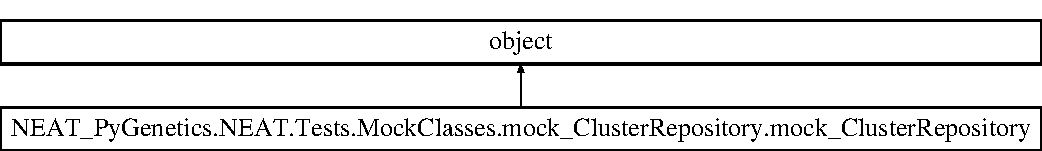
\includegraphics[height=2.000000cm]{classNEAT__PyGenetics_1_1NEAT_1_1Tests_1_1MockClasses_1_1mock__ClusterRepository_1_1mock__ClusterRepository}
\end{center}
\end{figure}
\subsection*{Public Member Functions}
\begin{DoxyCompactItemize}
\item 
def \hyperlink{classNEAT__PyGenetics_1_1NEAT_1_1Tests_1_1MockClasses_1_1mock__ClusterRepository_1_1mock__ClusterRepository_a9f89fd3f00cd01d78dcae1af7b061c8a}{\+\_\+\+\_\+init\+\_\+\+\_\+} (self)
\item 
def \hyperlink{classNEAT__PyGenetics_1_1NEAT_1_1Tests_1_1MockClasses_1_1mock__ClusterRepository_1_1mock__ClusterRepository_a7c1d0e1494945daece920c3faa393417}{reset} (self)
\item 
def \hyperlink{classNEAT__PyGenetics_1_1NEAT_1_1Tests_1_1MockClasses_1_1mock__ClusterRepository_1_1mock__ClusterRepository_aaedaee0f127d37e0c3a5521f15364277}{get\+\_\+cluster\+\_\+count} (self)
\item 
def \hyperlink{classNEAT__PyGenetics_1_1NEAT_1_1Tests_1_1MockClasses_1_1mock__ClusterRepository_1_1mock__ClusterRepository_a226b6c12fc2b76219c55c9e4b99baa16}{add\+\_\+cluster\+\_\+with\+\_\+representative}
\item 
def \hyperlink{classNEAT__PyGenetics_1_1NEAT_1_1Tests_1_1MockClasses_1_1mock__ClusterRepository_1_1mock__ClusterRepository_a134f5b068a5237328c7c3b481852bafd}{get\+\_\+current\+\_\+clusters} (self)
\item 
def \hyperlink{classNEAT__PyGenetics_1_1NEAT_1_1Tests_1_1MockClasses_1_1mock__ClusterRepository_1_1mock__ClusterRepository_abeb34604f2a2aa59c79c0db965494929}{get\+\_\+cluster\+\_\+by\+\_\+representative}
\item 
def \hyperlink{classNEAT__PyGenetics_1_1NEAT_1_1Tests_1_1MockClasses_1_1mock__ClusterRepository_1_1mock__ClusterRepository_aee0e3e9834f04db0768aefa4949fecdf}{update\+\_\+fitness\+\_\+for\+\_\+cluster}
\item 
def \hyperlink{classNEAT__PyGenetics_1_1NEAT_1_1Tests_1_1MockClasses_1_1mock__ClusterRepository_1_1mock__ClusterRepository_a750492b84023bed8ca6f78ccda904de5}{update\+\_\+max\+\_\+population\+\_\+for\+\_\+cluster}
\item 
def \hyperlink{classNEAT__PyGenetics_1_1NEAT_1_1Tests_1_1MockClasses_1_1mock__ClusterRepository_1_1mock__ClusterRepository_ac6f8854ca405235c472100f1b9519762}{update\+\_\+offspring\+\_\+for\+\_\+cluster}
\end{DoxyCompactItemize}
\subsection*{Public Attributes}
\begin{DoxyCompactItemize}
\item 
\hyperlink{classNEAT__PyGenetics_1_1NEAT_1_1Tests_1_1MockClasses_1_1mock__ClusterRepository_1_1mock__ClusterRepository_a2e2d77ba5375cceedf179e25c7887de5}{clusters}
\item 
\hyperlink{classNEAT__PyGenetics_1_1NEAT_1_1Tests_1_1MockClasses_1_1mock__ClusterRepository_1_1mock__ClusterRepository_a3b7a06a95cca18e535ce14621cd4fa4d}{next\+\_\+id}
\end{DoxyCompactItemize}


\subsection{Constructor \& Destructor Documentation}
\index{N\+E\+A\+T\+\_\+\+Py\+Genetics\+::\+N\+E\+A\+T\+::\+Tests\+::\+Mock\+Classes\+::mock\+\_\+\+Cluster\+Repository\+::mock\+\_\+\+Cluster\+Repository@{N\+E\+A\+T\+\_\+\+Py\+Genetics\+::\+N\+E\+A\+T\+::\+Tests\+::\+Mock\+Classes\+::mock\+\_\+\+Cluster\+Repository\+::mock\+\_\+\+Cluster\+Repository}!\+\_\+\+\_\+init\+\_\+\+\_\+@{\+\_\+\+\_\+init\+\_\+\+\_\+}}
\index{\+\_\+\+\_\+init\+\_\+\+\_\+@{\+\_\+\+\_\+init\+\_\+\+\_\+}!N\+E\+A\+T\+\_\+\+Py\+Genetics\+::\+N\+E\+A\+T\+::\+Tests\+::\+Mock\+Classes\+::mock\+\_\+\+Cluster\+Repository\+::mock\+\_\+\+Cluster\+Repository@{N\+E\+A\+T\+\_\+\+Py\+Genetics\+::\+N\+E\+A\+T\+::\+Tests\+::\+Mock\+Classes\+::mock\+\_\+\+Cluster\+Repository\+::mock\+\_\+\+Cluster\+Repository}}
\subsubsection[{\texorpdfstring{\+\_\+\+\_\+init\+\_\+\+\_\+(self)}{__init__(self)}}]{\setlength{\rightskip}{0pt plus 5cm}def N\+E\+A\+T\+\_\+\+Py\+Genetics.\+N\+E\+A\+T.\+Tests.\+Mock\+Classes.\+mock\+\_\+\+Cluster\+Repository.\+mock\+\_\+\+Cluster\+Repository.\+\_\+\+\_\+init\+\_\+\+\_\+ (
\begin{DoxyParamCaption}
\item[{}]{self}
\end{DoxyParamCaption}
)}\hypertarget{classNEAT__PyGenetics_1_1NEAT_1_1Tests_1_1MockClasses_1_1mock__ClusterRepository_1_1mock__ClusterRepository_a9f89fd3f00cd01d78dcae1af7b061c8a}{}\label{classNEAT__PyGenetics_1_1NEAT_1_1Tests_1_1MockClasses_1_1mock__ClusterRepository_1_1mock__ClusterRepository_a9f89fd3f00cd01d78dcae1af7b061c8a}


\subsection{Member Function Documentation}
\index{N\+E\+A\+T\+\_\+\+Py\+Genetics\+::\+N\+E\+A\+T\+::\+Tests\+::\+Mock\+Classes\+::mock\+\_\+\+Cluster\+Repository\+::mock\+\_\+\+Cluster\+Repository@{N\+E\+A\+T\+\_\+\+Py\+Genetics\+::\+N\+E\+A\+T\+::\+Tests\+::\+Mock\+Classes\+::mock\+\_\+\+Cluster\+Repository\+::mock\+\_\+\+Cluster\+Repository}!add\+\_\+cluster\+\_\+with\+\_\+representative@{add\+\_\+cluster\+\_\+with\+\_\+representative}}
\index{add\+\_\+cluster\+\_\+with\+\_\+representative@{add\+\_\+cluster\+\_\+with\+\_\+representative}!N\+E\+A\+T\+\_\+\+Py\+Genetics\+::\+N\+E\+A\+T\+::\+Tests\+::\+Mock\+Classes\+::mock\+\_\+\+Cluster\+Repository\+::mock\+\_\+\+Cluster\+Repository@{N\+E\+A\+T\+\_\+\+Py\+Genetics\+::\+N\+E\+A\+T\+::\+Tests\+::\+Mock\+Classes\+::mock\+\_\+\+Cluster\+Repository\+::mock\+\_\+\+Cluster\+Repository}}
\subsubsection[{\texorpdfstring{add\+\_\+cluster\+\_\+with\+\_\+representative}{add_cluster_with_representative}}]{\setlength{\rightskip}{0pt plus 5cm}def N\+E\+A\+T\+\_\+\+Py\+Genetics.\+N\+E\+A\+T.\+Tests.\+Mock\+Classes.\+mock\+\_\+\+Cluster\+Repository.\+mock\+\_\+\+Cluster\+Repository.\+add\+\_\+cluster\+\_\+with\+\_\+representative (
\begin{DoxyParamCaption}
\item[{}]{self, }
\item[{}]{genome\+\_\+id}
\end{DoxyParamCaption}
)}\hypertarget{classNEAT__PyGenetics_1_1NEAT_1_1Tests_1_1MockClasses_1_1mock__ClusterRepository_1_1mock__ClusterRepository_a226b6c12fc2b76219c55c9e4b99baa16}{}\label{classNEAT__PyGenetics_1_1NEAT_1_1Tests_1_1MockClasses_1_1mock__ClusterRepository_1_1mock__ClusterRepository_a226b6c12fc2b76219c55c9e4b99baa16}
\index{N\+E\+A\+T\+\_\+\+Py\+Genetics\+::\+N\+E\+A\+T\+::\+Tests\+::\+Mock\+Classes\+::mock\+\_\+\+Cluster\+Repository\+::mock\+\_\+\+Cluster\+Repository@{N\+E\+A\+T\+\_\+\+Py\+Genetics\+::\+N\+E\+A\+T\+::\+Tests\+::\+Mock\+Classes\+::mock\+\_\+\+Cluster\+Repository\+::mock\+\_\+\+Cluster\+Repository}!get\+\_\+cluster\+\_\+by\+\_\+representative@{get\+\_\+cluster\+\_\+by\+\_\+representative}}
\index{get\+\_\+cluster\+\_\+by\+\_\+representative@{get\+\_\+cluster\+\_\+by\+\_\+representative}!N\+E\+A\+T\+\_\+\+Py\+Genetics\+::\+N\+E\+A\+T\+::\+Tests\+::\+Mock\+Classes\+::mock\+\_\+\+Cluster\+Repository\+::mock\+\_\+\+Cluster\+Repository@{N\+E\+A\+T\+\_\+\+Py\+Genetics\+::\+N\+E\+A\+T\+::\+Tests\+::\+Mock\+Classes\+::mock\+\_\+\+Cluster\+Repository\+::mock\+\_\+\+Cluster\+Repository}}
\subsubsection[{\texorpdfstring{get\+\_\+cluster\+\_\+by\+\_\+representative}{get_cluster_by_representative}}]{\setlength{\rightskip}{0pt plus 5cm}def N\+E\+A\+T\+\_\+\+Py\+Genetics.\+N\+E\+A\+T.\+Tests.\+Mock\+Classes.\+mock\+\_\+\+Cluster\+Repository.\+mock\+\_\+\+Cluster\+Repository.\+get\+\_\+cluster\+\_\+by\+\_\+representative (
\begin{DoxyParamCaption}
\item[{}]{self, }
\item[{}]{genome\+\_\+id}
\end{DoxyParamCaption}
)}\hypertarget{classNEAT__PyGenetics_1_1NEAT_1_1Tests_1_1MockClasses_1_1mock__ClusterRepository_1_1mock__ClusterRepository_abeb34604f2a2aa59c79c0db965494929}{}\label{classNEAT__PyGenetics_1_1NEAT_1_1Tests_1_1MockClasses_1_1mock__ClusterRepository_1_1mock__ClusterRepository_abeb34604f2a2aa59c79c0db965494929}
\index{N\+E\+A\+T\+\_\+\+Py\+Genetics\+::\+N\+E\+A\+T\+::\+Tests\+::\+Mock\+Classes\+::mock\+\_\+\+Cluster\+Repository\+::mock\+\_\+\+Cluster\+Repository@{N\+E\+A\+T\+\_\+\+Py\+Genetics\+::\+N\+E\+A\+T\+::\+Tests\+::\+Mock\+Classes\+::mock\+\_\+\+Cluster\+Repository\+::mock\+\_\+\+Cluster\+Repository}!get\+\_\+cluster\+\_\+count@{get\+\_\+cluster\+\_\+count}}
\index{get\+\_\+cluster\+\_\+count@{get\+\_\+cluster\+\_\+count}!N\+E\+A\+T\+\_\+\+Py\+Genetics\+::\+N\+E\+A\+T\+::\+Tests\+::\+Mock\+Classes\+::mock\+\_\+\+Cluster\+Repository\+::mock\+\_\+\+Cluster\+Repository@{N\+E\+A\+T\+\_\+\+Py\+Genetics\+::\+N\+E\+A\+T\+::\+Tests\+::\+Mock\+Classes\+::mock\+\_\+\+Cluster\+Repository\+::mock\+\_\+\+Cluster\+Repository}}
\subsubsection[{\texorpdfstring{get\+\_\+cluster\+\_\+count(self)}{get_cluster_count(self)}}]{\setlength{\rightskip}{0pt plus 5cm}def N\+E\+A\+T\+\_\+\+Py\+Genetics.\+N\+E\+A\+T.\+Tests.\+Mock\+Classes.\+mock\+\_\+\+Cluster\+Repository.\+mock\+\_\+\+Cluster\+Repository.\+get\+\_\+cluster\+\_\+count (
\begin{DoxyParamCaption}
\item[{}]{self}
\end{DoxyParamCaption}
)}\hypertarget{classNEAT__PyGenetics_1_1NEAT_1_1Tests_1_1MockClasses_1_1mock__ClusterRepository_1_1mock__ClusterRepository_aaedaee0f127d37e0c3a5521f15364277}{}\label{classNEAT__PyGenetics_1_1NEAT_1_1Tests_1_1MockClasses_1_1mock__ClusterRepository_1_1mock__ClusterRepository_aaedaee0f127d37e0c3a5521f15364277}
\index{N\+E\+A\+T\+\_\+\+Py\+Genetics\+::\+N\+E\+A\+T\+::\+Tests\+::\+Mock\+Classes\+::mock\+\_\+\+Cluster\+Repository\+::mock\+\_\+\+Cluster\+Repository@{N\+E\+A\+T\+\_\+\+Py\+Genetics\+::\+N\+E\+A\+T\+::\+Tests\+::\+Mock\+Classes\+::mock\+\_\+\+Cluster\+Repository\+::mock\+\_\+\+Cluster\+Repository}!get\+\_\+current\+\_\+clusters@{get\+\_\+current\+\_\+clusters}}
\index{get\+\_\+current\+\_\+clusters@{get\+\_\+current\+\_\+clusters}!N\+E\+A\+T\+\_\+\+Py\+Genetics\+::\+N\+E\+A\+T\+::\+Tests\+::\+Mock\+Classes\+::mock\+\_\+\+Cluster\+Repository\+::mock\+\_\+\+Cluster\+Repository@{N\+E\+A\+T\+\_\+\+Py\+Genetics\+::\+N\+E\+A\+T\+::\+Tests\+::\+Mock\+Classes\+::mock\+\_\+\+Cluster\+Repository\+::mock\+\_\+\+Cluster\+Repository}}
\subsubsection[{\texorpdfstring{get\+\_\+current\+\_\+clusters(self)}{get_current_clusters(self)}}]{\setlength{\rightskip}{0pt plus 5cm}def N\+E\+A\+T\+\_\+\+Py\+Genetics.\+N\+E\+A\+T.\+Tests.\+Mock\+Classes.\+mock\+\_\+\+Cluster\+Repository.\+mock\+\_\+\+Cluster\+Repository.\+get\+\_\+current\+\_\+clusters (
\begin{DoxyParamCaption}
\item[{}]{self}
\end{DoxyParamCaption}
)}\hypertarget{classNEAT__PyGenetics_1_1NEAT_1_1Tests_1_1MockClasses_1_1mock__ClusterRepository_1_1mock__ClusterRepository_a134f5b068a5237328c7c3b481852bafd}{}\label{classNEAT__PyGenetics_1_1NEAT_1_1Tests_1_1MockClasses_1_1mock__ClusterRepository_1_1mock__ClusterRepository_a134f5b068a5237328c7c3b481852bafd}
\index{N\+E\+A\+T\+\_\+\+Py\+Genetics\+::\+N\+E\+A\+T\+::\+Tests\+::\+Mock\+Classes\+::mock\+\_\+\+Cluster\+Repository\+::mock\+\_\+\+Cluster\+Repository@{N\+E\+A\+T\+\_\+\+Py\+Genetics\+::\+N\+E\+A\+T\+::\+Tests\+::\+Mock\+Classes\+::mock\+\_\+\+Cluster\+Repository\+::mock\+\_\+\+Cluster\+Repository}!reset@{reset}}
\index{reset@{reset}!N\+E\+A\+T\+\_\+\+Py\+Genetics\+::\+N\+E\+A\+T\+::\+Tests\+::\+Mock\+Classes\+::mock\+\_\+\+Cluster\+Repository\+::mock\+\_\+\+Cluster\+Repository@{N\+E\+A\+T\+\_\+\+Py\+Genetics\+::\+N\+E\+A\+T\+::\+Tests\+::\+Mock\+Classes\+::mock\+\_\+\+Cluster\+Repository\+::mock\+\_\+\+Cluster\+Repository}}
\subsubsection[{\texorpdfstring{reset(self)}{reset(self)}}]{\setlength{\rightskip}{0pt plus 5cm}def N\+E\+A\+T\+\_\+\+Py\+Genetics.\+N\+E\+A\+T.\+Tests.\+Mock\+Classes.\+mock\+\_\+\+Cluster\+Repository.\+mock\+\_\+\+Cluster\+Repository.\+reset (
\begin{DoxyParamCaption}
\item[{}]{self}
\end{DoxyParamCaption}
)}\hypertarget{classNEAT__PyGenetics_1_1NEAT_1_1Tests_1_1MockClasses_1_1mock__ClusterRepository_1_1mock__ClusterRepository_a7c1d0e1494945daece920c3faa393417}{}\label{classNEAT__PyGenetics_1_1NEAT_1_1Tests_1_1MockClasses_1_1mock__ClusterRepository_1_1mock__ClusterRepository_a7c1d0e1494945daece920c3faa393417}
\index{N\+E\+A\+T\+\_\+\+Py\+Genetics\+::\+N\+E\+A\+T\+::\+Tests\+::\+Mock\+Classes\+::mock\+\_\+\+Cluster\+Repository\+::mock\+\_\+\+Cluster\+Repository@{N\+E\+A\+T\+\_\+\+Py\+Genetics\+::\+N\+E\+A\+T\+::\+Tests\+::\+Mock\+Classes\+::mock\+\_\+\+Cluster\+Repository\+::mock\+\_\+\+Cluster\+Repository}!update\+\_\+fitness\+\_\+for\+\_\+cluster@{update\+\_\+fitness\+\_\+for\+\_\+cluster}}
\index{update\+\_\+fitness\+\_\+for\+\_\+cluster@{update\+\_\+fitness\+\_\+for\+\_\+cluster}!N\+E\+A\+T\+\_\+\+Py\+Genetics\+::\+N\+E\+A\+T\+::\+Tests\+::\+Mock\+Classes\+::mock\+\_\+\+Cluster\+Repository\+::mock\+\_\+\+Cluster\+Repository@{N\+E\+A\+T\+\_\+\+Py\+Genetics\+::\+N\+E\+A\+T\+::\+Tests\+::\+Mock\+Classes\+::mock\+\_\+\+Cluster\+Repository\+::mock\+\_\+\+Cluster\+Repository}}
\subsubsection[{\texorpdfstring{update\+\_\+fitness\+\_\+for\+\_\+cluster}{update_fitness_for_cluster}}]{\setlength{\rightskip}{0pt plus 5cm}def N\+E\+A\+T\+\_\+\+Py\+Genetics.\+N\+E\+A\+T.\+Tests.\+Mock\+Classes.\+mock\+\_\+\+Cluster\+Repository.\+mock\+\_\+\+Cluster\+Repository.\+update\+\_\+fitness\+\_\+for\+\_\+cluster (
\begin{DoxyParamCaption}
\item[{}]{self, }
\item[{}]{cluster\+\_\+id}
\end{DoxyParamCaption}
)}\hypertarget{classNEAT__PyGenetics_1_1NEAT_1_1Tests_1_1MockClasses_1_1mock__ClusterRepository_1_1mock__ClusterRepository_aee0e3e9834f04db0768aefa4949fecdf}{}\label{classNEAT__PyGenetics_1_1NEAT_1_1Tests_1_1MockClasses_1_1mock__ClusterRepository_1_1mock__ClusterRepository_aee0e3e9834f04db0768aefa4949fecdf}
\index{N\+E\+A\+T\+\_\+\+Py\+Genetics\+::\+N\+E\+A\+T\+::\+Tests\+::\+Mock\+Classes\+::mock\+\_\+\+Cluster\+Repository\+::mock\+\_\+\+Cluster\+Repository@{N\+E\+A\+T\+\_\+\+Py\+Genetics\+::\+N\+E\+A\+T\+::\+Tests\+::\+Mock\+Classes\+::mock\+\_\+\+Cluster\+Repository\+::mock\+\_\+\+Cluster\+Repository}!update\+\_\+max\+\_\+population\+\_\+for\+\_\+cluster@{update\+\_\+max\+\_\+population\+\_\+for\+\_\+cluster}}
\index{update\+\_\+max\+\_\+population\+\_\+for\+\_\+cluster@{update\+\_\+max\+\_\+population\+\_\+for\+\_\+cluster}!N\+E\+A\+T\+\_\+\+Py\+Genetics\+::\+N\+E\+A\+T\+::\+Tests\+::\+Mock\+Classes\+::mock\+\_\+\+Cluster\+Repository\+::mock\+\_\+\+Cluster\+Repository@{N\+E\+A\+T\+\_\+\+Py\+Genetics\+::\+N\+E\+A\+T\+::\+Tests\+::\+Mock\+Classes\+::mock\+\_\+\+Cluster\+Repository\+::mock\+\_\+\+Cluster\+Repository}}
\subsubsection[{\texorpdfstring{update\+\_\+max\+\_\+population\+\_\+for\+\_\+cluster}{update_max_population_for_cluster}}]{\setlength{\rightskip}{0pt plus 5cm}def N\+E\+A\+T\+\_\+\+Py\+Genetics.\+N\+E\+A\+T.\+Tests.\+Mock\+Classes.\+mock\+\_\+\+Cluster\+Repository.\+mock\+\_\+\+Cluster\+Repository.\+update\+\_\+max\+\_\+population\+\_\+for\+\_\+cluster (
\begin{DoxyParamCaption}
\item[{}]{self, }
\item[{}]{cluster\+\_\+id}
\end{DoxyParamCaption}
)}\hypertarget{classNEAT__PyGenetics_1_1NEAT_1_1Tests_1_1MockClasses_1_1mock__ClusterRepository_1_1mock__ClusterRepository_a750492b84023bed8ca6f78ccda904de5}{}\label{classNEAT__PyGenetics_1_1NEAT_1_1Tests_1_1MockClasses_1_1mock__ClusterRepository_1_1mock__ClusterRepository_a750492b84023bed8ca6f78ccda904de5}
\index{N\+E\+A\+T\+\_\+\+Py\+Genetics\+::\+N\+E\+A\+T\+::\+Tests\+::\+Mock\+Classes\+::mock\+\_\+\+Cluster\+Repository\+::mock\+\_\+\+Cluster\+Repository@{N\+E\+A\+T\+\_\+\+Py\+Genetics\+::\+N\+E\+A\+T\+::\+Tests\+::\+Mock\+Classes\+::mock\+\_\+\+Cluster\+Repository\+::mock\+\_\+\+Cluster\+Repository}!update\+\_\+offspring\+\_\+for\+\_\+cluster@{update\+\_\+offspring\+\_\+for\+\_\+cluster}}
\index{update\+\_\+offspring\+\_\+for\+\_\+cluster@{update\+\_\+offspring\+\_\+for\+\_\+cluster}!N\+E\+A\+T\+\_\+\+Py\+Genetics\+::\+N\+E\+A\+T\+::\+Tests\+::\+Mock\+Classes\+::mock\+\_\+\+Cluster\+Repository\+::mock\+\_\+\+Cluster\+Repository@{N\+E\+A\+T\+\_\+\+Py\+Genetics\+::\+N\+E\+A\+T\+::\+Tests\+::\+Mock\+Classes\+::mock\+\_\+\+Cluster\+Repository\+::mock\+\_\+\+Cluster\+Repository}}
\subsubsection[{\texorpdfstring{update\+\_\+offspring\+\_\+for\+\_\+cluster}{update_offspring_for_cluster}}]{\setlength{\rightskip}{0pt plus 5cm}def N\+E\+A\+T\+\_\+\+Py\+Genetics.\+N\+E\+A\+T.\+Tests.\+Mock\+Classes.\+mock\+\_\+\+Cluster\+Repository.\+mock\+\_\+\+Cluster\+Repository.\+update\+\_\+offspring\+\_\+for\+\_\+cluster (
\begin{DoxyParamCaption}
\item[{}]{self, }
\item[{}]{cluster\+\_\+id}
\end{DoxyParamCaption}
)}\hypertarget{classNEAT__PyGenetics_1_1NEAT_1_1Tests_1_1MockClasses_1_1mock__ClusterRepository_1_1mock__ClusterRepository_ac6f8854ca405235c472100f1b9519762}{}\label{classNEAT__PyGenetics_1_1NEAT_1_1Tests_1_1MockClasses_1_1mock__ClusterRepository_1_1mock__ClusterRepository_ac6f8854ca405235c472100f1b9519762}


\subsection{Member Data Documentation}
\index{N\+E\+A\+T\+\_\+\+Py\+Genetics\+::\+N\+E\+A\+T\+::\+Tests\+::\+Mock\+Classes\+::mock\+\_\+\+Cluster\+Repository\+::mock\+\_\+\+Cluster\+Repository@{N\+E\+A\+T\+\_\+\+Py\+Genetics\+::\+N\+E\+A\+T\+::\+Tests\+::\+Mock\+Classes\+::mock\+\_\+\+Cluster\+Repository\+::mock\+\_\+\+Cluster\+Repository}!clusters@{clusters}}
\index{clusters@{clusters}!N\+E\+A\+T\+\_\+\+Py\+Genetics\+::\+N\+E\+A\+T\+::\+Tests\+::\+Mock\+Classes\+::mock\+\_\+\+Cluster\+Repository\+::mock\+\_\+\+Cluster\+Repository@{N\+E\+A\+T\+\_\+\+Py\+Genetics\+::\+N\+E\+A\+T\+::\+Tests\+::\+Mock\+Classes\+::mock\+\_\+\+Cluster\+Repository\+::mock\+\_\+\+Cluster\+Repository}}
\subsubsection[{\texorpdfstring{clusters}{clusters}}]{\setlength{\rightskip}{0pt plus 5cm}N\+E\+A\+T\+\_\+\+Py\+Genetics.\+N\+E\+A\+T.\+Tests.\+Mock\+Classes.\+mock\+\_\+\+Cluster\+Repository.\+mock\+\_\+\+Cluster\+Repository.\+clusters}\hypertarget{classNEAT__PyGenetics_1_1NEAT_1_1Tests_1_1MockClasses_1_1mock__ClusterRepository_1_1mock__ClusterRepository_a2e2d77ba5375cceedf179e25c7887de5}{}\label{classNEAT__PyGenetics_1_1NEAT_1_1Tests_1_1MockClasses_1_1mock__ClusterRepository_1_1mock__ClusterRepository_a2e2d77ba5375cceedf179e25c7887de5}
\index{N\+E\+A\+T\+\_\+\+Py\+Genetics\+::\+N\+E\+A\+T\+::\+Tests\+::\+Mock\+Classes\+::mock\+\_\+\+Cluster\+Repository\+::mock\+\_\+\+Cluster\+Repository@{N\+E\+A\+T\+\_\+\+Py\+Genetics\+::\+N\+E\+A\+T\+::\+Tests\+::\+Mock\+Classes\+::mock\+\_\+\+Cluster\+Repository\+::mock\+\_\+\+Cluster\+Repository}!next\+\_\+id@{next\+\_\+id}}
\index{next\+\_\+id@{next\+\_\+id}!N\+E\+A\+T\+\_\+\+Py\+Genetics\+::\+N\+E\+A\+T\+::\+Tests\+::\+Mock\+Classes\+::mock\+\_\+\+Cluster\+Repository\+::mock\+\_\+\+Cluster\+Repository@{N\+E\+A\+T\+\_\+\+Py\+Genetics\+::\+N\+E\+A\+T\+::\+Tests\+::\+Mock\+Classes\+::mock\+\_\+\+Cluster\+Repository\+::mock\+\_\+\+Cluster\+Repository}}
\subsubsection[{\texorpdfstring{next\+\_\+id}{next_id}}]{\setlength{\rightskip}{0pt plus 5cm}N\+E\+A\+T\+\_\+\+Py\+Genetics.\+N\+E\+A\+T.\+Tests.\+Mock\+Classes.\+mock\+\_\+\+Cluster\+Repository.\+mock\+\_\+\+Cluster\+Repository.\+next\+\_\+id}\hypertarget{classNEAT__PyGenetics_1_1NEAT_1_1Tests_1_1MockClasses_1_1mock__ClusterRepository_1_1mock__ClusterRepository_a3b7a06a95cca18e535ce14621cd4fa4d}{}\label{classNEAT__PyGenetics_1_1NEAT_1_1Tests_1_1MockClasses_1_1mock__ClusterRepository_1_1mock__ClusterRepository_a3b7a06a95cca18e535ce14621cd4fa4d}


The documentation for this class was generated from the following file\+:\begin{DoxyCompactItemize}
\item 
N\+E\+A\+T/\+Tests/\+Mock\+Classes/\hyperlink{mock__ClusterRepository_8py}{mock\+\_\+\+Cluster\+Repository.\+py}\end{DoxyCompactItemize}

\hypertarget{classNEAT__PyGenetics_1_1NEAT_1_1Tests_1_1MockClasses_1_1mock__DatabaseConnector_1_1mock__DatabaseConnector}{}\section{N\+E\+A\+T\+\_\+\+Py\+Genetics.\+N\+E\+A\+T.\+Tests.\+Mock\+Classes.\+mock\+\_\+\+Database\+Connector.\+mock\+\_\+\+Database\+Connector Class Reference}
\label{classNEAT__PyGenetics_1_1NEAT_1_1Tests_1_1MockClasses_1_1mock__DatabaseConnector_1_1mock__DatabaseConnector}\index{N\+E\+A\+T\+\_\+\+Py\+Genetics.\+N\+E\+A\+T.\+Tests.\+Mock\+Classes.\+mock\+\_\+\+Database\+Connector.\+mock\+\_\+\+Database\+Connector@{N\+E\+A\+T\+\_\+\+Py\+Genetics.\+N\+E\+A\+T.\+Tests.\+Mock\+Classes.\+mock\+\_\+\+Database\+Connector.\+mock\+\_\+\+Database\+Connector}}
Inheritance diagram for N\+E\+A\+T\+\_\+\+Py\+Genetics.\+N\+E\+A\+T.\+Tests.\+Mock\+Classes.\+mock\+\_\+\+Database\+Connector.\+mock\+\_\+\+Database\+Connector\+:\begin{figure}[H]
\begin{center}
\leavevmode
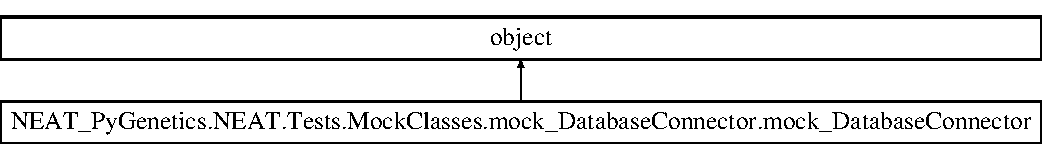
\includegraphics[height=1.941074cm]{classNEAT__PyGenetics_1_1NEAT_1_1Tests_1_1MockClasses_1_1mock__DatabaseConnector_1_1mock__DatabaseConnector}
\end{center}
\end{figure}
\subsection*{Public Member Functions}
\begin{DoxyCompactItemize}
\item 
def \hyperlink{classNEAT__PyGenetics_1_1NEAT_1_1Tests_1_1MockClasses_1_1mock__DatabaseConnector_1_1mock__DatabaseConnector_a02398d61ab2bab01e548b901cd4d70f7}{\+\_\+\+\_\+init\+\_\+\+\_\+} (self)
\item 
def \hyperlink{classNEAT__PyGenetics_1_1NEAT_1_1Tests_1_1MockClasses_1_1mock__DatabaseConnector_1_1mock__DatabaseConnector_aef1a53517f1680bcc5ddfcbeff3f4785}{get\+\_\+collection}
\item 
def \hyperlink{classNEAT__PyGenetics_1_1NEAT_1_1Tests_1_1MockClasses_1_1mock__DatabaseConnector_1_1mock__DatabaseConnector_a9f8c8a2adf0987729548df63dfe118e8}{insert\+\_\+one}
\item 
def \hyperlink{classNEAT__PyGenetics_1_1NEAT_1_1Tests_1_1MockClasses_1_1mock__DatabaseConnector_1_1mock__DatabaseConnector_a0c7202b51bd1bf1001d3748ac39d825b}{insert\+\_\+many}
\item 
def \hyperlink{classNEAT__PyGenetics_1_1NEAT_1_1Tests_1_1MockClasses_1_1mock__DatabaseConnector_1_1mock__DatabaseConnector_ac03ab8b0c7fda497eac3ca7435aec3a0}{find\+\_\+one}
\item 
def \hyperlink{classNEAT__PyGenetics_1_1NEAT_1_1Tests_1_1MockClasses_1_1mock__DatabaseConnector_1_1mock__DatabaseConnector_ace6331811ba2e674ef037a66d073377a}{find\+\_\+one\+\_\+by\+\_\+id}
\item 
def \hyperlink{classNEAT__PyGenetics_1_1NEAT_1_1Tests_1_1MockClasses_1_1mock__DatabaseConnector_1_1mock__DatabaseConnector_a0ea2557b31cd7af3af9e098cc8dd3f7d}{find\+\_\+many}
\item 
def \hyperlink{classNEAT__PyGenetics_1_1NEAT_1_1Tests_1_1MockClasses_1_1mock__DatabaseConnector_1_1mock__DatabaseConnector_a01f612634b7f3da00fb1b327dfa5b524}{update\+\_\+one}
\item 
def \hyperlink{classNEAT__PyGenetics_1_1NEAT_1_1Tests_1_1MockClasses_1_1mock__DatabaseConnector_1_1mock__DatabaseConnector_a9fa32e7c0e425396238b66ab8f3ffb5e}{update\+\_\+many}
\item 
def \hyperlink{classNEAT__PyGenetics_1_1NEAT_1_1Tests_1_1MockClasses_1_1mock__DatabaseConnector_1_1mock__DatabaseConnector_a534ae334b83f54bce7d32f66faf22440}{remove\+\_\+one}
\item 
def \hyperlink{classNEAT__PyGenetics_1_1NEAT_1_1Tests_1_1MockClasses_1_1mock__DatabaseConnector_1_1mock__DatabaseConnector_ab3ff82b4de49e912a56c7b3cd0a208ac}{remove\+\_\+many}
\item 
def \hyperlink{classNEAT__PyGenetics_1_1NEAT_1_1Tests_1_1MockClasses_1_1mock__DatabaseConnector_1_1mock__DatabaseConnector_a9092111a34ce0573dace98120682e415}{create\+\_\+collection\+\_\+if\+\_\+not\+\_\+exists} (self, collection\+\_\+name)
\item 
def \hyperlink{classNEAT__PyGenetics_1_1NEAT_1_1Tests_1_1MockClasses_1_1mock__DatabaseConnector_1_1mock__DatabaseConnector_a7172e251a453e9481d7c8359b6961105}{next\+\_\+id} (self)
\end{DoxyCompactItemize}
\subsection*{Static Public Attributes}
\begin{DoxyCompactItemize}
\item 
\hyperlink{classNEAT__PyGenetics_1_1NEAT_1_1Tests_1_1MockClasses_1_1mock__DatabaseConnector_1_1mock__DatabaseConnector_aaa8b3d15b7e01aef04c5ab3f58e8a006}{assigned\+\_\+id}
\item 
\hyperlink{classNEAT__PyGenetics_1_1NEAT_1_1Tests_1_1MockClasses_1_1mock__DatabaseConnector_1_1mock__DatabaseConnector_a6061ac8abee52f8e6d81b92c24c944eb}{assigned\+\_\+ids}
\item 
\hyperlink{classNEAT__PyGenetics_1_1NEAT_1_1Tests_1_1MockClasses_1_1mock__DatabaseConnector_1_1mock__DatabaseConnector_a7e65d11937c1858690f2cd25ac07de18}{filter\+\_\+mismatch}
\item 
\hyperlink{classNEAT__PyGenetics_1_1NEAT_1_1Tests_1_1MockClasses_1_1mock__DatabaseConnector_1_1mock__DatabaseConnector_a3370fecdccb2abc0c0a3356825f04cc4}{results}
\end{DoxyCompactItemize}


\subsection{Constructor \& Destructor Documentation}
\index{N\+E\+A\+T\+\_\+\+Py\+Genetics\+::\+N\+E\+A\+T\+::\+Tests\+::\+Mock\+Classes\+::mock\+\_\+\+Database\+Connector\+::mock\+\_\+\+Database\+Connector@{N\+E\+A\+T\+\_\+\+Py\+Genetics\+::\+N\+E\+A\+T\+::\+Tests\+::\+Mock\+Classes\+::mock\+\_\+\+Database\+Connector\+::mock\+\_\+\+Database\+Connector}!\+\_\+\+\_\+init\+\_\+\+\_\+@{\+\_\+\+\_\+init\+\_\+\+\_\+}}
\index{\+\_\+\+\_\+init\+\_\+\+\_\+@{\+\_\+\+\_\+init\+\_\+\+\_\+}!N\+E\+A\+T\+\_\+\+Py\+Genetics\+::\+N\+E\+A\+T\+::\+Tests\+::\+Mock\+Classes\+::mock\+\_\+\+Database\+Connector\+::mock\+\_\+\+Database\+Connector@{N\+E\+A\+T\+\_\+\+Py\+Genetics\+::\+N\+E\+A\+T\+::\+Tests\+::\+Mock\+Classes\+::mock\+\_\+\+Database\+Connector\+::mock\+\_\+\+Database\+Connector}}
\subsubsection[{\texorpdfstring{\+\_\+\+\_\+init\+\_\+\+\_\+(self)}{__init__(self)}}]{\setlength{\rightskip}{0pt plus 5cm}def N\+E\+A\+T\+\_\+\+Py\+Genetics.\+N\+E\+A\+T.\+Tests.\+Mock\+Classes.\+mock\+\_\+\+Database\+Connector.\+mock\+\_\+\+Database\+Connector.\+\_\+\+\_\+init\+\_\+\+\_\+ (
\begin{DoxyParamCaption}
\item[{}]{self}
\end{DoxyParamCaption}
)}\hypertarget{classNEAT__PyGenetics_1_1NEAT_1_1Tests_1_1MockClasses_1_1mock__DatabaseConnector_1_1mock__DatabaseConnector_a02398d61ab2bab01e548b901cd4d70f7}{}\label{classNEAT__PyGenetics_1_1NEAT_1_1Tests_1_1MockClasses_1_1mock__DatabaseConnector_1_1mock__DatabaseConnector_a02398d61ab2bab01e548b901cd4d70f7}


\subsection{Member Function Documentation}
\index{N\+E\+A\+T\+\_\+\+Py\+Genetics\+::\+N\+E\+A\+T\+::\+Tests\+::\+Mock\+Classes\+::mock\+\_\+\+Database\+Connector\+::mock\+\_\+\+Database\+Connector@{N\+E\+A\+T\+\_\+\+Py\+Genetics\+::\+N\+E\+A\+T\+::\+Tests\+::\+Mock\+Classes\+::mock\+\_\+\+Database\+Connector\+::mock\+\_\+\+Database\+Connector}!create\+\_\+collection\+\_\+if\+\_\+not\+\_\+exists@{create\+\_\+collection\+\_\+if\+\_\+not\+\_\+exists}}
\index{create\+\_\+collection\+\_\+if\+\_\+not\+\_\+exists@{create\+\_\+collection\+\_\+if\+\_\+not\+\_\+exists}!N\+E\+A\+T\+\_\+\+Py\+Genetics\+::\+N\+E\+A\+T\+::\+Tests\+::\+Mock\+Classes\+::mock\+\_\+\+Database\+Connector\+::mock\+\_\+\+Database\+Connector@{N\+E\+A\+T\+\_\+\+Py\+Genetics\+::\+N\+E\+A\+T\+::\+Tests\+::\+Mock\+Classes\+::mock\+\_\+\+Database\+Connector\+::mock\+\_\+\+Database\+Connector}}
\subsubsection[{\texorpdfstring{create\+\_\+collection\+\_\+if\+\_\+not\+\_\+exists(self, collection\+\_\+name)}{create_collection_if_not_exists(self, collection_name)}}]{\setlength{\rightskip}{0pt plus 5cm}def N\+E\+A\+T\+\_\+\+Py\+Genetics.\+N\+E\+A\+T.\+Tests.\+Mock\+Classes.\+mock\+\_\+\+Database\+Connector.\+mock\+\_\+\+Database\+Connector.\+create\+\_\+collection\+\_\+if\+\_\+not\+\_\+exists (
\begin{DoxyParamCaption}
\item[{}]{self, }
\item[{}]{collection\+\_\+name}
\end{DoxyParamCaption}
)}\hypertarget{classNEAT__PyGenetics_1_1NEAT_1_1Tests_1_1MockClasses_1_1mock__DatabaseConnector_1_1mock__DatabaseConnector_a9092111a34ce0573dace98120682e415}{}\label{classNEAT__PyGenetics_1_1NEAT_1_1Tests_1_1MockClasses_1_1mock__DatabaseConnector_1_1mock__DatabaseConnector_a9092111a34ce0573dace98120682e415}
\index{N\+E\+A\+T\+\_\+\+Py\+Genetics\+::\+N\+E\+A\+T\+::\+Tests\+::\+Mock\+Classes\+::mock\+\_\+\+Database\+Connector\+::mock\+\_\+\+Database\+Connector@{N\+E\+A\+T\+\_\+\+Py\+Genetics\+::\+N\+E\+A\+T\+::\+Tests\+::\+Mock\+Classes\+::mock\+\_\+\+Database\+Connector\+::mock\+\_\+\+Database\+Connector}!find\+\_\+many@{find\+\_\+many}}
\index{find\+\_\+many@{find\+\_\+many}!N\+E\+A\+T\+\_\+\+Py\+Genetics\+::\+N\+E\+A\+T\+::\+Tests\+::\+Mock\+Classes\+::mock\+\_\+\+Database\+Connector\+::mock\+\_\+\+Database\+Connector@{N\+E\+A\+T\+\_\+\+Py\+Genetics\+::\+N\+E\+A\+T\+::\+Tests\+::\+Mock\+Classes\+::mock\+\_\+\+Database\+Connector\+::mock\+\_\+\+Database\+Connector}}
\subsubsection[{\texorpdfstring{find\+\_\+many}{find_many}}]{\setlength{\rightskip}{0pt plus 5cm}def N\+E\+A\+T\+\_\+\+Py\+Genetics.\+N\+E\+A\+T.\+Tests.\+Mock\+Classes.\+mock\+\_\+\+Database\+Connector.\+mock\+\_\+\+Database\+Connector.\+find\+\_\+many (
\begin{DoxyParamCaption}
\item[{}]{self, }
\item[{}]{collection\+\_\+name}
\end{DoxyParamCaption}
)}\hypertarget{classNEAT__PyGenetics_1_1NEAT_1_1Tests_1_1MockClasses_1_1mock__DatabaseConnector_1_1mock__DatabaseConnector_a0ea2557b31cd7af3af9e098cc8dd3f7d}{}\label{classNEAT__PyGenetics_1_1NEAT_1_1Tests_1_1MockClasses_1_1mock__DatabaseConnector_1_1mock__DatabaseConnector_a0ea2557b31cd7af3af9e098cc8dd3f7d}
\index{N\+E\+A\+T\+\_\+\+Py\+Genetics\+::\+N\+E\+A\+T\+::\+Tests\+::\+Mock\+Classes\+::mock\+\_\+\+Database\+Connector\+::mock\+\_\+\+Database\+Connector@{N\+E\+A\+T\+\_\+\+Py\+Genetics\+::\+N\+E\+A\+T\+::\+Tests\+::\+Mock\+Classes\+::mock\+\_\+\+Database\+Connector\+::mock\+\_\+\+Database\+Connector}!find\+\_\+one@{find\+\_\+one}}
\index{find\+\_\+one@{find\+\_\+one}!N\+E\+A\+T\+\_\+\+Py\+Genetics\+::\+N\+E\+A\+T\+::\+Tests\+::\+Mock\+Classes\+::mock\+\_\+\+Database\+Connector\+::mock\+\_\+\+Database\+Connector@{N\+E\+A\+T\+\_\+\+Py\+Genetics\+::\+N\+E\+A\+T\+::\+Tests\+::\+Mock\+Classes\+::mock\+\_\+\+Database\+Connector\+::mock\+\_\+\+Database\+Connector}}
\subsubsection[{\texorpdfstring{find\+\_\+one}{find_one}}]{\setlength{\rightskip}{0pt plus 5cm}def N\+E\+A\+T\+\_\+\+Py\+Genetics.\+N\+E\+A\+T.\+Tests.\+Mock\+Classes.\+mock\+\_\+\+Database\+Connector.\+mock\+\_\+\+Database\+Connector.\+find\+\_\+one (
\begin{DoxyParamCaption}
\item[{}]{self, }
\item[{}]{collection\+\_\+name}
\end{DoxyParamCaption}
)}\hypertarget{classNEAT__PyGenetics_1_1NEAT_1_1Tests_1_1MockClasses_1_1mock__DatabaseConnector_1_1mock__DatabaseConnector_ac03ab8b0c7fda497eac3ca7435aec3a0}{}\label{classNEAT__PyGenetics_1_1NEAT_1_1Tests_1_1MockClasses_1_1mock__DatabaseConnector_1_1mock__DatabaseConnector_ac03ab8b0c7fda497eac3ca7435aec3a0}
\index{N\+E\+A\+T\+\_\+\+Py\+Genetics\+::\+N\+E\+A\+T\+::\+Tests\+::\+Mock\+Classes\+::mock\+\_\+\+Database\+Connector\+::mock\+\_\+\+Database\+Connector@{N\+E\+A\+T\+\_\+\+Py\+Genetics\+::\+N\+E\+A\+T\+::\+Tests\+::\+Mock\+Classes\+::mock\+\_\+\+Database\+Connector\+::mock\+\_\+\+Database\+Connector}!find\+\_\+one\+\_\+by\+\_\+id@{find\+\_\+one\+\_\+by\+\_\+id}}
\index{find\+\_\+one\+\_\+by\+\_\+id@{find\+\_\+one\+\_\+by\+\_\+id}!N\+E\+A\+T\+\_\+\+Py\+Genetics\+::\+N\+E\+A\+T\+::\+Tests\+::\+Mock\+Classes\+::mock\+\_\+\+Database\+Connector\+::mock\+\_\+\+Database\+Connector@{N\+E\+A\+T\+\_\+\+Py\+Genetics\+::\+N\+E\+A\+T\+::\+Tests\+::\+Mock\+Classes\+::mock\+\_\+\+Database\+Connector\+::mock\+\_\+\+Database\+Connector}}
\subsubsection[{\texorpdfstring{find\+\_\+one\+\_\+by\+\_\+id}{find_one_by_id}}]{\setlength{\rightskip}{0pt plus 5cm}def N\+E\+A\+T\+\_\+\+Py\+Genetics.\+N\+E\+A\+T.\+Tests.\+Mock\+Classes.\+mock\+\_\+\+Database\+Connector.\+mock\+\_\+\+Database\+Connector.\+find\+\_\+one\+\_\+by\+\_\+id (
\begin{DoxyParamCaption}
\item[{}]{self, }
\item[{}]{collection\+\_\+name}
\end{DoxyParamCaption}
)}\hypertarget{classNEAT__PyGenetics_1_1NEAT_1_1Tests_1_1MockClasses_1_1mock__DatabaseConnector_1_1mock__DatabaseConnector_ace6331811ba2e674ef037a66d073377a}{}\label{classNEAT__PyGenetics_1_1NEAT_1_1Tests_1_1MockClasses_1_1mock__DatabaseConnector_1_1mock__DatabaseConnector_ace6331811ba2e674ef037a66d073377a}
\index{N\+E\+A\+T\+\_\+\+Py\+Genetics\+::\+N\+E\+A\+T\+::\+Tests\+::\+Mock\+Classes\+::mock\+\_\+\+Database\+Connector\+::mock\+\_\+\+Database\+Connector@{N\+E\+A\+T\+\_\+\+Py\+Genetics\+::\+N\+E\+A\+T\+::\+Tests\+::\+Mock\+Classes\+::mock\+\_\+\+Database\+Connector\+::mock\+\_\+\+Database\+Connector}!get\+\_\+collection@{get\+\_\+collection}}
\index{get\+\_\+collection@{get\+\_\+collection}!N\+E\+A\+T\+\_\+\+Py\+Genetics\+::\+N\+E\+A\+T\+::\+Tests\+::\+Mock\+Classes\+::mock\+\_\+\+Database\+Connector\+::mock\+\_\+\+Database\+Connector@{N\+E\+A\+T\+\_\+\+Py\+Genetics\+::\+N\+E\+A\+T\+::\+Tests\+::\+Mock\+Classes\+::mock\+\_\+\+Database\+Connector\+::mock\+\_\+\+Database\+Connector}}
\subsubsection[{\texorpdfstring{get\+\_\+collection}{get_collection}}]{\setlength{\rightskip}{0pt plus 5cm}def N\+E\+A\+T\+\_\+\+Py\+Genetics.\+N\+E\+A\+T.\+Tests.\+Mock\+Classes.\+mock\+\_\+\+Database\+Connector.\+mock\+\_\+\+Database\+Connector.\+get\+\_\+collection (
\begin{DoxyParamCaption}
\item[{}]{self, }
\item[{}]{collection\+\_\+name}
\end{DoxyParamCaption}
)}\hypertarget{classNEAT__PyGenetics_1_1NEAT_1_1Tests_1_1MockClasses_1_1mock__DatabaseConnector_1_1mock__DatabaseConnector_aef1a53517f1680bcc5ddfcbeff3f4785}{}\label{classNEAT__PyGenetics_1_1NEAT_1_1Tests_1_1MockClasses_1_1mock__DatabaseConnector_1_1mock__DatabaseConnector_aef1a53517f1680bcc5ddfcbeff3f4785}
\index{N\+E\+A\+T\+\_\+\+Py\+Genetics\+::\+N\+E\+A\+T\+::\+Tests\+::\+Mock\+Classes\+::mock\+\_\+\+Database\+Connector\+::mock\+\_\+\+Database\+Connector@{N\+E\+A\+T\+\_\+\+Py\+Genetics\+::\+N\+E\+A\+T\+::\+Tests\+::\+Mock\+Classes\+::mock\+\_\+\+Database\+Connector\+::mock\+\_\+\+Database\+Connector}!insert\+\_\+many@{insert\+\_\+many}}
\index{insert\+\_\+many@{insert\+\_\+many}!N\+E\+A\+T\+\_\+\+Py\+Genetics\+::\+N\+E\+A\+T\+::\+Tests\+::\+Mock\+Classes\+::mock\+\_\+\+Database\+Connector\+::mock\+\_\+\+Database\+Connector@{N\+E\+A\+T\+\_\+\+Py\+Genetics\+::\+N\+E\+A\+T\+::\+Tests\+::\+Mock\+Classes\+::mock\+\_\+\+Database\+Connector\+::mock\+\_\+\+Database\+Connector}}
\subsubsection[{\texorpdfstring{insert\+\_\+many}{insert_many}}]{\setlength{\rightskip}{0pt plus 5cm}def N\+E\+A\+T\+\_\+\+Py\+Genetics.\+N\+E\+A\+T.\+Tests.\+Mock\+Classes.\+mock\+\_\+\+Database\+Connector.\+mock\+\_\+\+Database\+Connector.\+insert\+\_\+many (
\begin{DoxyParamCaption}
\item[{}]{self, }
\item[{}]{collection\+\_\+name}
\end{DoxyParamCaption}
)}\hypertarget{classNEAT__PyGenetics_1_1NEAT_1_1Tests_1_1MockClasses_1_1mock__DatabaseConnector_1_1mock__DatabaseConnector_a0c7202b51bd1bf1001d3748ac39d825b}{}\label{classNEAT__PyGenetics_1_1NEAT_1_1Tests_1_1MockClasses_1_1mock__DatabaseConnector_1_1mock__DatabaseConnector_a0c7202b51bd1bf1001d3748ac39d825b}
\index{N\+E\+A\+T\+\_\+\+Py\+Genetics\+::\+N\+E\+A\+T\+::\+Tests\+::\+Mock\+Classes\+::mock\+\_\+\+Database\+Connector\+::mock\+\_\+\+Database\+Connector@{N\+E\+A\+T\+\_\+\+Py\+Genetics\+::\+N\+E\+A\+T\+::\+Tests\+::\+Mock\+Classes\+::mock\+\_\+\+Database\+Connector\+::mock\+\_\+\+Database\+Connector}!insert\+\_\+one@{insert\+\_\+one}}
\index{insert\+\_\+one@{insert\+\_\+one}!N\+E\+A\+T\+\_\+\+Py\+Genetics\+::\+N\+E\+A\+T\+::\+Tests\+::\+Mock\+Classes\+::mock\+\_\+\+Database\+Connector\+::mock\+\_\+\+Database\+Connector@{N\+E\+A\+T\+\_\+\+Py\+Genetics\+::\+N\+E\+A\+T\+::\+Tests\+::\+Mock\+Classes\+::mock\+\_\+\+Database\+Connector\+::mock\+\_\+\+Database\+Connector}}
\subsubsection[{\texorpdfstring{insert\+\_\+one}{insert_one}}]{\setlength{\rightskip}{0pt plus 5cm}def N\+E\+A\+T\+\_\+\+Py\+Genetics.\+N\+E\+A\+T.\+Tests.\+Mock\+Classes.\+mock\+\_\+\+Database\+Connector.\+mock\+\_\+\+Database\+Connector.\+insert\+\_\+one (
\begin{DoxyParamCaption}
\item[{}]{self, }
\item[{}]{collection\+\_\+name}
\end{DoxyParamCaption}
)}\hypertarget{classNEAT__PyGenetics_1_1NEAT_1_1Tests_1_1MockClasses_1_1mock__DatabaseConnector_1_1mock__DatabaseConnector_a9f8c8a2adf0987729548df63dfe118e8}{}\label{classNEAT__PyGenetics_1_1NEAT_1_1Tests_1_1MockClasses_1_1mock__DatabaseConnector_1_1mock__DatabaseConnector_a9f8c8a2adf0987729548df63dfe118e8}
\index{N\+E\+A\+T\+\_\+\+Py\+Genetics\+::\+N\+E\+A\+T\+::\+Tests\+::\+Mock\+Classes\+::mock\+\_\+\+Database\+Connector\+::mock\+\_\+\+Database\+Connector@{N\+E\+A\+T\+\_\+\+Py\+Genetics\+::\+N\+E\+A\+T\+::\+Tests\+::\+Mock\+Classes\+::mock\+\_\+\+Database\+Connector\+::mock\+\_\+\+Database\+Connector}!next\+\_\+id@{next\+\_\+id}}
\index{next\+\_\+id@{next\+\_\+id}!N\+E\+A\+T\+\_\+\+Py\+Genetics\+::\+N\+E\+A\+T\+::\+Tests\+::\+Mock\+Classes\+::mock\+\_\+\+Database\+Connector\+::mock\+\_\+\+Database\+Connector@{N\+E\+A\+T\+\_\+\+Py\+Genetics\+::\+N\+E\+A\+T\+::\+Tests\+::\+Mock\+Classes\+::mock\+\_\+\+Database\+Connector\+::mock\+\_\+\+Database\+Connector}}
\subsubsection[{\texorpdfstring{next\+\_\+id(self)}{next_id(self)}}]{\setlength{\rightskip}{0pt plus 5cm}def N\+E\+A\+T\+\_\+\+Py\+Genetics.\+N\+E\+A\+T.\+Tests.\+Mock\+Classes.\+mock\+\_\+\+Database\+Connector.\+mock\+\_\+\+Database\+Connector.\+next\+\_\+id (
\begin{DoxyParamCaption}
\item[{}]{self}
\end{DoxyParamCaption}
)}\hypertarget{classNEAT__PyGenetics_1_1NEAT_1_1Tests_1_1MockClasses_1_1mock__DatabaseConnector_1_1mock__DatabaseConnector_a7172e251a453e9481d7c8359b6961105}{}\label{classNEAT__PyGenetics_1_1NEAT_1_1Tests_1_1MockClasses_1_1mock__DatabaseConnector_1_1mock__DatabaseConnector_a7172e251a453e9481d7c8359b6961105}
\index{N\+E\+A\+T\+\_\+\+Py\+Genetics\+::\+N\+E\+A\+T\+::\+Tests\+::\+Mock\+Classes\+::mock\+\_\+\+Database\+Connector\+::mock\+\_\+\+Database\+Connector@{N\+E\+A\+T\+\_\+\+Py\+Genetics\+::\+N\+E\+A\+T\+::\+Tests\+::\+Mock\+Classes\+::mock\+\_\+\+Database\+Connector\+::mock\+\_\+\+Database\+Connector}!remove\+\_\+many@{remove\+\_\+many}}
\index{remove\+\_\+many@{remove\+\_\+many}!N\+E\+A\+T\+\_\+\+Py\+Genetics\+::\+N\+E\+A\+T\+::\+Tests\+::\+Mock\+Classes\+::mock\+\_\+\+Database\+Connector\+::mock\+\_\+\+Database\+Connector@{N\+E\+A\+T\+\_\+\+Py\+Genetics\+::\+N\+E\+A\+T\+::\+Tests\+::\+Mock\+Classes\+::mock\+\_\+\+Database\+Connector\+::mock\+\_\+\+Database\+Connector}}
\subsubsection[{\texorpdfstring{remove\+\_\+many}{remove_many}}]{\setlength{\rightskip}{0pt plus 5cm}def N\+E\+A\+T\+\_\+\+Py\+Genetics.\+N\+E\+A\+T.\+Tests.\+Mock\+Classes.\+mock\+\_\+\+Database\+Connector.\+mock\+\_\+\+Database\+Connector.\+remove\+\_\+many (
\begin{DoxyParamCaption}
\item[{}]{self, }
\item[{}]{collection\+\_\+name}
\end{DoxyParamCaption}
)}\hypertarget{classNEAT__PyGenetics_1_1NEAT_1_1Tests_1_1MockClasses_1_1mock__DatabaseConnector_1_1mock__DatabaseConnector_ab3ff82b4de49e912a56c7b3cd0a208ac}{}\label{classNEAT__PyGenetics_1_1NEAT_1_1Tests_1_1MockClasses_1_1mock__DatabaseConnector_1_1mock__DatabaseConnector_ab3ff82b4de49e912a56c7b3cd0a208ac}
\index{N\+E\+A\+T\+\_\+\+Py\+Genetics\+::\+N\+E\+A\+T\+::\+Tests\+::\+Mock\+Classes\+::mock\+\_\+\+Database\+Connector\+::mock\+\_\+\+Database\+Connector@{N\+E\+A\+T\+\_\+\+Py\+Genetics\+::\+N\+E\+A\+T\+::\+Tests\+::\+Mock\+Classes\+::mock\+\_\+\+Database\+Connector\+::mock\+\_\+\+Database\+Connector}!remove\+\_\+one@{remove\+\_\+one}}
\index{remove\+\_\+one@{remove\+\_\+one}!N\+E\+A\+T\+\_\+\+Py\+Genetics\+::\+N\+E\+A\+T\+::\+Tests\+::\+Mock\+Classes\+::mock\+\_\+\+Database\+Connector\+::mock\+\_\+\+Database\+Connector@{N\+E\+A\+T\+\_\+\+Py\+Genetics\+::\+N\+E\+A\+T\+::\+Tests\+::\+Mock\+Classes\+::mock\+\_\+\+Database\+Connector\+::mock\+\_\+\+Database\+Connector}}
\subsubsection[{\texorpdfstring{remove\+\_\+one}{remove_one}}]{\setlength{\rightskip}{0pt plus 5cm}def N\+E\+A\+T\+\_\+\+Py\+Genetics.\+N\+E\+A\+T.\+Tests.\+Mock\+Classes.\+mock\+\_\+\+Database\+Connector.\+mock\+\_\+\+Database\+Connector.\+remove\+\_\+one (
\begin{DoxyParamCaption}
\item[{}]{self, }
\item[{}]{collection\+\_\+name}
\end{DoxyParamCaption}
)}\hypertarget{classNEAT__PyGenetics_1_1NEAT_1_1Tests_1_1MockClasses_1_1mock__DatabaseConnector_1_1mock__DatabaseConnector_a534ae334b83f54bce7d32f66faf22440}{}\label{classNEAT__PyGenetics_1_1NEAT_1_1Tests_1_1MockClasses_1_1mock__DatabaseConnector_1_1mock__DatabaseConnector_a534ae334b83f54bce7d32f66faf22440}
\index{N\+E\+A\+T\+\_\+\+Py\+Genetics\+::\+N\+E\+A\+T\+::\+Tests\+::\+Mock\+Classes\+::mock\+\_\+\+Database\+Connector\+::mock\+\_\+\+Database\+Connector@{N\+E\+A\+T\+\_\+\+Py\+Genetics\+::\+N\+E\+A\+T\+::\+Tests\+::\+Mock\+Classes\+::mock\+\_\+\+Database\+Connector\+::mock\+\_\+\+Database\+Connector}!update\+\_\+many@{update\+\_\+many}}
\index{update\+\_\+many@{update\+\_\+many}!N\+E\+A\+T\+\_\+\+Py\+Genetics\+::\+N\+E\+A\+T\+::\+Tests\+::\+Mock\+Classes\+::mock\+\_\+\+Database\+Connector\+::mock\+\_\+\+Database\+Connector@{N\+E\+A\+T\+\_\+\+Py\+Genetics\+::\+N\+E\+A\+T\+::\+Tests\+::\+Mock\+Classes\+::mock\+\_\+\+Database\+Connector\+::mock\+\_\+\+Database\+Connector}}
\subsubsection[{\texorpdfstring{update\+\_\+many}{update_many}}]{\setlength{\rightskip}{0pt plus 5cm}def N\+E\+A\+T\+\_\+\+Py\+Genetics.\+N\+E\+A\+T.\+Tests.\+Mock\+Classes.\+mock\+\_\+\+Database\+Connector.\+mock\+\_\+\+Database\+Connector.\+update\+\_\+many (
\begin{DoxyParamCaption}
\item[{}]{self, }
\item[{}]{collection\+\_\+name}
\end{DoxyParamCaption}
)}\hypertarget{classNEAT__PyGenetics_1_1NEAT_1_1Tests_1_1MockClasses_1_1mock__DatabaseConnector_1_1mock__DatabaseConnector_a9fa32e7c0e425396238b66ab8f3ffb5e}{}\label{classNEAT__PyGenetics_1_1NEAT_1_1Tests_1_1MockClasses_1_1mock__DatabaseConnector_1_1mock__DatabaseConnector_a9fa32e7c0e425396238b66ab8f3ffb5e}
\index{N\+E\+A\+T\+\_\+\+Py\+Genetics\+::\+N\+E\+A\+T\+::\+Tests\+::\+Mock\+Classes\+::mock\+\_\+\+Database\+Connector\+::mock\+\_\+\+Database\+Connector@{N\+E\+A\+T\+\_\+\+Py\+Genetics\+::\+N\+E\+A\+T\+::\+Tests\+::\+Mock\+Classes\+::mock\+\_\+\+Database\+Connector\+::mock\+\_\+\+Database\+Connector}!update\+\_\+one@{update\+\_\+one}}
\index{update\+\_\+one@{update\+\_\+one}!N\+E\+A\+T\+\_\+\+Py\+Genetics\+::\+N\+E\+A\+T\+::\+Tests\+::\+Mock\+Classes\+::mock\+\_\+\+Database\+Connector\+::mock\+\_\+\+Database\+Connector@{N\+E\+A\+T\+\_\+\+Py\+Genetics\+::\+N\+E\+A\+T\+::\+Tests\+::\+Mock\+Classes\+::mock\+\_\+\+Database\+Connector\+::mock\+\_\+\+Database\+Connector}}
\subsubsection[{\texorpdfstring{update\+\_\+one}{update_one}}]{\setlength{\rightskip}{0pt plus 5cm}def N\+E\+A\+T\+\_\+\+Py\+Genetics.\+N\+E\+A\+T.\+Tests.\+Mock\+Classes.\+mock\+\_\+\+Database\+Connector.\+mock\+\_\+\+Database\+Connector.\+update\+\_\+one (
\begin{DoxyParamCaption}
\item[{}]{self, }
\item[{}]{collection\+\_\+name}
\end{DoxyParamCaption}
)}\hypertarget{classNEAT__PyGenetics_1_1NEAT_1_1Tests_1_1MockClasses_1_1mock__DatabaseConnector_1_1mock__DatabaseConnector_a01f612634b7f3da00fb1b327dfa5b524}{}\label{classNEAT__PyGenetics_1_1NEAT_1_1Tests_1_1MockClasses_1_1mock__DatabaseConnector_1_1mock__DatabaseConnector_a01f612634b7f3da00fb1b327dfa5b524}


\subsection{Member Data Documentation}
\index{N\+E\+A\+T\+\_\+\+Py\+Genetics\+::\+N\+E\+A\+T\+::\+Tests\+::\+Mock\+Classes\+::mock\+\_\+\+Database\+Connector\+::mock\+\_\+\+Database\+Connector@{N\+E\+A\+T\+\_\+\+Py\+Genetics\+::\+N\+E\+A\+T\+::\+Tests\+::\+Mock\+Classes\+::mock\+\_\+\+Database\+Connector\+::mock\+\_\+\+Database\+Connector}!assigned\+\_\+id@{assigned\+\_\+id}}
\index{assigned\+\_\+id@{assigned\+\_\+id}!N\+E\+A\+T\+\_\+\+Py\+Genetics\+::\+N\+E\+A\+T\+::\+Tests\+::\+Mock\+Classes\+::mock\+\_\+\+Database\+Connector\+::mock\+\_\+\+Database\+Connector@{N\+E\+A\+T\+\_\+\+Py\+Genetics\+::\+N\+E\+A\+T\+::\+Tests\+::\+Mock\+Classes\+::mock\+\_\+\+Database\+Connector\+::mock\+\_\+\+Database\+Connector}}
\subsubsection[{\texorpdfstring{assigned\+\_\+id}{assigned_id}}]{\setlength{\rightskip}{0pt plus 5cm}N\+E\+A\+T\+\_\+\+Py\+Genetics.\+N\+E\+A\+T.\+Tests.\+Mock\+Classes.\+mock\+\_\+\+Database\+Connector.\+mock\+\_\+\+Database\+Connector.\+assigned\+\_\+id\hspace{0.3cm}{\ttfamily [static]}}\hypertarget{classNEAT__PyGenetics_1_1NEAT_1_1Tests_1_1MockClasses_1_1mock__DatabaseConnector_1_1mock__DatabaseConnector_aaa8b3d15b7e01aef04c5ab3f58e8a006}{}\label{classNEAT__PyGenetics_1_1NEAT_1_1Tests_1_1MockClasses_1_1mock__DatabaseConnector_1_1mock__DatabaseConnector_aaa8b3d15b7e01aef04c5ab3f58e8a006}
\index{N\+E\+A\+T\+\_\+\+Py\+Genetics\+::\+N\+E\+A\+T\+::\+Tests\+::\+Mock\+Classes\+::mock\+\_\+\+Database\+Connector\+::mock\+\_\+\+Database\+Connector@{N\+E\+A\+T\+\_\+\+Py\+Genetics\+::\+N\+E\+A\+T\+::\+Tests\+::\+Mock\+Classes\+::mock\+\_\+\+Database\+Connector\+::mock\+\_\+\+Database\+Connector}!assigned\+\_\+ids@{assigned\+\_\+ids}}
\index{assigned\+\_\+ids@{assigned\+\_\+ids}!N\+E\+A\+T\+\_\+\+Py\+Genetics\+::\+N\+E\+A\+T\+::\+Tests\+::\+Mock\+Classes\+::mock\+\_\+\+Database\+Connector\+::mock\+\_\+\+Database\+Connector@{N\+E\+A\+T\+\_\+\+Py\+Genetics\+::\+N\+E\+A\+T\+::\+Tests\+::\+Mock\+Classes\+::mock\+\_\+\+Database\+Connector\+::mock\+\_\+\+Database\+Connector}}
\subsubsection[{\texorpdfstring{assigned\+\_\+ids}{assigned_ids}}]{\setlength{\rightskip}{0pt plus 5cm}N\+E\+A\+T\+\_\+\+Py\+Genetics.\+N\+E\+A\+T.\+Tests.\+Mock\+Classes.\+mock\+\_\+\+Database\+Connector.\+mock\+\_\+\+Database\+Connector.\+assigned\+\_\+ids\hspace{0.3cm}{\ttfamily [static]}}\hypertarget{classNEAT__PyGenetics_1_1NEAT_1_1Tests_1_1MockClasses_1_1mock__DatabaseConnector_1_1mock__DatabaseConnector_a6061ac8abee52f8e6d81b92c24c944eb}{}\label{classNEAT__PyGenetics_1_1NEAT_1_1Tests_1_1MockClasses_1_1mock__DatabaseConnector_1_1mock__DatabaseConnector_a6061ac8abee52f8e6d81b92c24c944eb}
\index{N\+E\+A\+T\+\_\+\+Py\+Genetics\+::\+N\+E\+A\+T\+::\+Tests\+::\+Mock\+Classes\+::mock\+\_\+\+Database\+Connector\+::mock\+\_\+\+Database\+Connector@{N\+E\+A\+T\+\_\+\+Py\+Genetics\+::\+N\+E\+A\+T\+::\+Tests\+::\+Mock\+Classes\+::mock\+\_\+\+Database\+Connector\+::mock\+\_\+\+Database\+Connector}!filter\+\_\+mismatch@{filter\+\_\+mismatch}}
\index{filter\+\_\+mismatch@{filter\+\_\+mismatch}!N\+E\+A\+T\+\_\+\+Py\+Genetics\+::\+N\+E\+A\+T\+::\+Tests\+::\+Mock\+Classes\+::mock\+\_\+\+Database\+Connector\+::mock\+\_\+\+Database\+Connector@{N\+E\+A\+T\+\_\+\+Py\+Genetics\+::\+N\+E\+A\+T\+::\+Tests\+::\+Mock\+Classes\+::mock\+\_\+\+Database\+Connector\+::mock\+\_\+\+Database\+Connector}}
\subsubsection[{\texorpdfstring{filter\+\_\+mismatch}{filter_mismatch}}]{\setlength{\rightskip}{0pt plus 5cm}N\+E\+A\+T\+\_\+\+Py\+Genetics.\+N\+E\+A\+T.\+Tests.\+Mock\+Classes.\+mock\+\_\+\+Database\+Connector.\+mock\+\_\+\+Database\+Connector.\+filter\+\_\+mismatch\hspace{0.3cm}{\ttfamily [static]}}\hypertarget{classNEAT__PyGenetics_1_1NEAT_1_1Tests_1_1MockClasses_1_1mock__DatabaseConnector_1_1mock__DatabaseConnector_a7e65d11937c1858690f2cd25ac07de18}{}\label{classNEAT__PyGenetics_1_1NEAT_1_1Tests_1_1MockClasses_1_1mock__DatabaseConnector_1_1mock__DatabaseConnector_a7e65d11937c1858690f2cd25ac07de18}
\index{N\+E\+A\+T\+\_\+\+Py\+Genetics\+::\+N\+E\+A\+T\+::\+Tests\+::\+Mock\+Classes\+::mock\+\_\+\+Database\+Connector\+::mock\+\_\+\+Database\+Connector@{N\+E\+A\+T\+\_\+\+Py\+Genetics\+::\+N\+E\+A\+T\+::\+Tests\+::\+Mock\+Classes\+::mock\+\_\+\+Database\+Connector\+::mock\+\_\+\+Database\+Connector}!results@{results}}
\index{results@{results}!N\+E\+A\+T\+\_\+\+Py\+Genetics\+::\+N\+E\+A\+T\+::\+Tests\+::\+Mock\+Classes\+::mock\+\_\+\+Database\+Connector\+::mock\+\_\+\+Database\+Connector@{N\+E\+A\+T\+\_\+\+Py\+Genetics\+::\+N\+E\+A\+T\+::\+Tests\+::\+Mock\+Classes\+::mock\+\_\+\+Database\+Connector\+::mock\+\_\+\+Database\+Connector}}
\subsubsection[{\texorpdfstring{results}{results}}]{\setlength{\rightskip}{0pt plus 5cm}N\+E\+A\+T\+\_\+\+Py\+Genetics.\+N\+E\+A\+T.\+Tests.\+Mock\+Classes.\+mock\+\_\+\+Database\+Connector.\+mock\+\_\+\+Database\+Connector.\+results\hspace{0.3cm}{\ttfamily [static]}}\hypertarget{classNEAT__PyGenetics_1_1NEAT_1_1Tests_1_1MockClasses_1_1mock__DatabaseConnector_1_1mock__DatabaseConnector_a3370fecdccb2abc0c0a3356825f04cc4}{}\label{classNEAT__PyGenetics_1_1NEAT_1_1Tests_1_1MockClasses_1_1mock__DatabaseConnector_1_1mock__DatabaseConnector_a3370fecdccb2abc0c0a3356825f04cc4}


The documentation for this class was generated from the following file\+:\begin{DoxyCompactItemize}
\item 
N\+E\+A\+T/\+Tests/\+Mock\+Classes/\hyperlink{mock__DatabaseConnector_8py}{mock\+\_\+\+Database\+Connector.\+py}\end{DoxyCompactItemize}

\hypertarget{classNEAT__PyGenetics_1_1NEAT_1_1Tests_1_1MockClasses_1_1mock__GeneRepository_1_1mock__GeneRepository}{}\section{N\+E\+A\+T\+\_\+\+Py\+Genetics.\+N\+E\+A\+T.\+Tests.\+Mock\+Classes.\+mock\+\_\+\+Gene\+Repository.\+mock\+\_\+\+Gene\+Repository Class Reference}
\label{classNEAT__PyGenetics_1_1NEAT_1_1Tests_1_1MockClasses_1_1mock__GeneRepository_1_1mock__GeneRepository}\index{N\+E\+A\+T\+\_\+\+Py\+Genetics.\+N\+E\+A\+T.\+Tests.\+Mock\+Classes.\+mock\+\_\+\+Gene\+Repository.\+mock\+\_\+\+Gene\+Repository@{N\+E\+A\+T\+\_\+\+Py\+Genetics.\+N\+E\+A\+T.\+Tests.\+Mock\+Classes.\+mock\+\_\+\+Gene\+Repository.\+mock\+\_\+\+Gene\+Repository}}
Inheritance diagram for N\+E\+A\+T\+\_\+\+Py\+Genetics.\+N\+E\+A\+T.\+Tests.\+Mock\+Classes.\+mock\+\_\+\+Gene\+Repository.\+mock\+\_\+\+Gene\+Repository\+:\begin{figure}[H]
\begin{center}
\leavevmode
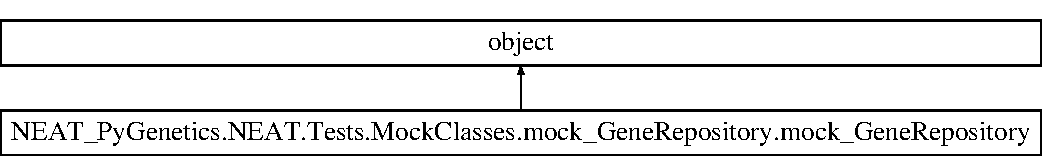
\includegraphics[height=2.000000cm]{classNEAT__PyGenetics_1_1NEAT_1_1Tests_1_1MockClasses_1_1mock__GeneRepository_1_1mock__GeneRepository}
\end{center}
\end{figure}
\subsection*{Public Member Functions}
\begin{DoxyCompactItemize}
\item 
def \hyperlink{classNEAT__PyGenetics_1_1NEAT_1_1Tests_1_1MockClasses_1_1mock__GeneRepository_1_1mock__GeneRepository_a7b5eef06e8d2486c49acb86b74f43316}{get\+\_\+gene\+\_\+id\+\_\+for\+\_\+endpoints} (self, head\+\_\+node\+\_\+id, tail\+\_\+node\+\_\+id)
\item 
def \hyperlink{classNEAT__PyGenetics_1_1NEAT_1_1Tests_1_1MockClasses_1_1mock__GeneRepository_1_1mock__GeneRepository_af8237f68a2528e68c6984225bc9a116f}{find\+\_\+connecting\+\_\+node} (self, head\+\_\+node\+\_\+id, tail\+\_\+node\+\_\+id)
\item 
def \hyperlink{classNEAT__PyGenetics_1_1NEAT_1_1Tests_1_1MockClasses_1_1mock__GeneRepository_1_1mock__GeneRepository_a496072cac2263f4b7213ba45f4458883}{get\+\_\+next\+\_\+node\+\_\+id} (self)
\end{DoxyCompactItemize}


\subsection{Member Function Documentation}
\index{N\+E\+A\+T\+\_\+\+Py\+Genetics\+::\+N\+E\+A\+T\+::\+Tests\+::\+Mock\+Classes\+::mock\+\_\+\+Gene\+Repository\+::mock\+\_\+\+Gene\+Repository@{N\+E\+A\+T\+\_\+\+Py\+Genetics\+::\+N\+E\+A\+T\+::\+Tests\+::\+Mock\+Classes\+::mock\+\_\+\+Gene\+Repository\+::mock\+\_\+\+Gene\+Repository}!find\+\_\+connecting\+\_\+node@{find\+\_\+connecting\+\_\+node}}
\index{find\+\_\+connecting\+\_\+node@{find\+\_\+connecting\+\_\+node}!N\+E\+A\+T\+\_\+\+Py\+Genetics\+::\+N\+E\+A\+T\+::\+Tests\+::\+Mock\+Classes\+::mock\+\_\+\+Gene\+Repository\+::mock\+\_\+\+Gene\+Repository@{N\+E\+A\+T\+\_\+\+Py\+Genetics\+::\+N\+E\+A\+T\+::\+Tests\+::\+Mock\+Classes\+::mock\+\_\+\+Gene\+Repository\+::mock\+\_\+\+Gene\+Repository}}
\subsubsection[{\texorpdfstring{find\+\_\+connecting\+\_\+node(self, head\+\_\+node\+\_\+id, tail\+\_\+node\+\_\+id)}{find_connecting_node(self, head_node_id, tail_node_id)}}]{\setlength{\rightskip}{0pt plus 5cm}def N\+E\+A\+T\+\_\+\+Py\+Genetics.\+N\+E\+A\+T.\+Tests.\+Mock\+Classes.\+mock\+\_\+\+Gene\+Repository.\+mock\+\_\+\+Gene\+Repository.\+find\+\_\+connecting\+\_\+node (
\begin{DoxyParamCaption}
\item[{}]{self, }
\item[{}]{head\+\_\+node\+\_\+id, }
\item[{}]{tail\+\_\+node\+\_\+id}
\end{DoxyParamCaption}
)}\hypertarget{classNEAT__PyGenetics_1_1NEAT_1_1Tests_1_1MockClasses_1_1mock__GeneRepository_1_1mock__GeneRepository_af8237f68a2528e68c6984225bc9a116f}{}\label{classNEAT__PyGenetics_1_1NEAT_1_1Tests_1_1MockClasses_1_1mock__GeneRepository_1_1mock__GeneRepository_af8237f68a2528e68c6984225bc9a116f}
\index{N\+E\+A\+T\+\_\+\+Py\+Genetics\+::\+N\+E\+A\+T\+::\+Tests\+::\+Mock\+Classes\+::mock\+\_\+\+Gene\+Repository\+::mock\+\_\+\+Gene\+Repository@{N\+E\+A\+T\+\_\+\+Py\+Genetics\+::\+N\+E\+A\+T\+::\+Tests\+::\+Mock\+Classes\+::mock\+\_\+\+Gene\+Repository\+::mock\+\_\+\+Gene\+Repository}!get\+\_\+gene\+\_\+id\+\_\+for\+\_\+endpoints@{get\+\_\+gene\+\_\+id\+\_\+for\+\_\+endpoints}}
\index{get\+\_\+gene\+\_\+id\+\_\+for\+\_\+endpoints@{get\+\_\+gene\+\_\+id\+\_\+for\+\_\+endpoints}!N\+E\+A\+T\+\_\+\+Py\+Genetics\+::\+N\+E\+A\+T\+::\+Tests\+::\+Mock\+Classes\+::mock\+\_\+\+Gene\+Repository\+::mock\+\_\+\+Gene\+Repository@{N\+E\+A\+T\+\_\+\+Py\+Genetics\+::\+N\+E\+A\+T\+::\+Tests\+::\+Mock\+Classes\+::mock\+\_\+\+Gene\+Repository\+::mock\+\_\+\+Gene\+Repository}}
\subsubsection[{\texorpdfstring{get\+\_\+gene\+\_\+id\+\_\+for\+\_\+endpoints(self, head\+\_\+node\+\_\+id, tail\+\_\+node\+\_\+id)}{get_gene_id_for_endpoints(self, head_node_id, tail_node_id)}}]{\setlength{\rightskip}{0pt plus 5cm}def N\+E\+A\+T\+\_\+\+Py\+Genetics.\+N\+E\+A\+T.\+Tests.\+Mock\+Classes.\+mock\+\_\+\+Gene\+Repository.\+mock\+\_\+\+Gene\+Repository.\+get\+\_\+gene\+\_\+id\+\_\+for\+\_\+endpoints (
\begin{DoxyParamCaption}
\item[{}]{self, }
\item[{}]{head\+\_\+node\+\_\+id, }
\item[{}]{tail\+\_\+node\+\_\+id}
\end{DoxyParamCaption}
)}\hypertarget{classNEAT__PyGenetics_1_1NEAT_1_1Tests_1_1MockClasses_1_1mock__GeneRepository_1_1mock__GeneRepository_a7b5eef06e8d2486c49acb86b74f43316}{}\label{classNEAT__PyGenetics_1_1NEAT_1_1Tests_1_1MockClasses_1_1mock__GeneRepository_1_1mock__GeneRepository_a7b5eef06e8d2486c49acb86b74f43316}
\index{N\+E\+A\+T\+\_\+\+Py\+Genetics\+::\+N\+E\+A\+T\+::\+Tests\+::\+Mock\+Classes\+::mock\+\_\+\+Gene\+Repository\+::mock\+\_\+\+Gene\+Repository@{N\+E\+A\+T\+\_\+\+Py\+Genetics\+::\+N\+E\+A\+T\+::\+Tests\+::\+Mock\+Classes\+::mock\+\_\+\+Gene\+Repository\+::mock\+\_\+\+Gene\+Repository}!get\+\_\+next\+\_\+node\+\_\+id@{get\+\_\+next\+\_\+node\+\_\+id}}
\index{get\+\_\+next\+\_\+node\+\_\+id@{get\+\_\+next\+\_\+node\+\_\+id}!N\+E\+A\+T\+\_\+\+Py\+Genetics\+::\+N\+E\+A\+T\+::\+Tests\+::\+Mock\+Classes\+::mock\+\_\+\+Gene\+Repository\+::mock\+\_\+\+Gene\+Repository@{N\+E\+A\+T\+\_\+\+Py\+Genetics\+::\+N\+E\+A\+T\+::\+Tests\+::\+Mock\+Classes\+::mock\+\_\+\+Gene\+Repository\+::mock\+\_\+\+Gene\+Repository}}
\subsubsection[{\texorpdfstring{get\+\_\+next\+\_\+node\+\_\+id(self)}{get_next_node_id(self)}}]{\setlength{\rightskip}{0pt plus 5cm}def N\+E\+A\+T\+\_\+\+Py\+Genetics.\+N\+E\+A\+T.\+Tests.\+Mock\+Classes.\+mock\+\_\+\+Gene\+Repository.\+mock\+\_\+\+Gene\+Repository.\+get\+\_\+next\+\_\+node\+\_\+id (
\begin{DoxyParamCaption}
\item[{}]{self}
\end{DoxyParamCaption}
)}\hypertarget{classNEAT__PyGenetics_1_1NEAT_1_1Tests_1_1MockClasses_1_1mock__GeneRepository_1_1mock__GeneRepository_a496072cac2263f4b7213ba45f4458883}{}\label{classNEAT__PyGenetics_1_1NEAT_1_1Tests_1_1MockClasses_1_1mock__GeneRepository_1_1mock__GeneRepository_a496072cac2263f4b7213ba45f4458883}


The documentation for this class was generated from the following file\+:\begin{DoxyCompactItemize}
\item 
N\+E\+A\+T/\+Tests/\+Mock\+Classes/\hyperlink{mock__GeneRepository_8py}{mock\+\_\+\+Gene\+Repository.\+py}\end{DoxyCompactItemize}

\hypertarget{classNEAT__PyGenetics_1_1NEAT_1_1Tests_1_1MockClasses_1_1mock__GenomeRepository_1_1mock__GenomeRepository}{}\section{N\+E\+A\+T\+\_\+\+Py\+Genetics.\+N\+E\+A\+T.\+Tests.\+Mock\+Classes.\+mock\+\_\+\+Genome\+Repository.\+mock\+\_\+\+Genome\+Repository Class Reference}
\label{classNEAT__PyGenetics_1_1NEAT_1_1Tests_1_1MockClasses_1_1mock__GenomeRepository_1_1mock__GenomeRepository}\index{N\+E\+A\+T\+\_\+\+Py\+Genetics.\+N\+E\+A\+T.\+Tests.\+Mock\+Classes.\+mock\+\_\+\+Genome\+Repository.\+mock\+\_\+\+Genome\+Repository@{N\+E\+A\+T\+\_\+\+Py\+Genetics.\+N\+E\+A\+T.\+Tests.\+Mock\+Classes.\+mock\+\_\+\+Genome\+Repository.\+mock\+\_\+\+Genome\+Repository}}
Inheritance diagram for N\+E\+A\+T\+\_\+\+Py\+Genetics.\+N\+E\+A\+T.\+Tests.\+Mock\+Classes.\+mock\+\_\+\+Genome\+Repository.\+mock\+\_\+\+Genome\+Repository\+:\begin{figure}[H]
\begin{center}
\leavevmode
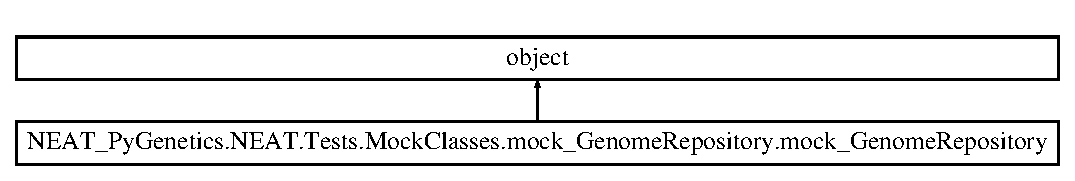
\includegraphics[height=1.982301cm]{classNEAT__PyGenetics_1_1NEAT_1_1Tests_1_1MockClasses_1_1mock__GenomeRepository_1_1mock__GenomeRepository}
\end{center}
\end{figure}
\subsection*{Public Member Functions}
\begin{DoxyCompactItemize}
\item 
def \hyperlink{classNEAT__PyGenetics_1_1NEAT_1_1Tests_1_1MockClasses_1_1mock__GenomeRepository_1_1mock__GenomeRepository_a1b6913e42019740f0dd683eef2bf8f32}{\+\_\+\+\_\+init\+\_\+\+\_\+} (self)
\item 
def \hyperlink{classNEAT__PyGenetics_1_1NEAT_1_1Tests_1_1MockClasses_1_1mock__GenomeRepository_1_1mock__GenomeRepository_ad5413865b1a0a82964e0046d59406383}{get\+\_\+current\+\_\+population} (self)
\item 
def \hyperlink{classNEAT__PyGenetics_1_1NEAT_1_1Tests_1_1MockClasses_1_1mock__GenomeRepository_1_1mock__GenomeRepository_a3d3a5d43fa4285aa6282557fef12f471}{update\+\_\+cluster\+\_\+for\+\_\+genome}
\item 
def \hyperlink{classNEAT__PyGenetics_1_1NEAT_1_1Tests_1_1MockClasses_1_1mock__GenomeRepository_1_1mock__GenomeRepository_aab8cb8b23202bf0a41e3dcbf42c096b0}{get\+\_\+genome\+\_\+by\+\_\+id}
\item 
def \hyperlink{classNEAT__PyGenetics_1_1NEAT_1_1Tests_1_1MockClasses_1_1mock__GenomeRepository_1_1mock__GenomeRepository_a5abad1601614b0c128b4ab64e41ecba8}{get\+\_\+genomes\+\_\+in\+\_\+cluster}
\end{DoxyCompactItemize}
\subsection*{Public Attributes}
\begin{DoxyCompactItemize}
\item 
\hyperlink{classNEAT__PyGenetics_1_1NEAT_1_1Tests_1_1MockClasses_1_1mock__GenomeRepository_1_1mock__GenomeRepository_abb2dfb4fa59c22b09dede3bcbd27ca4b}{mock\+\_\+population}
\end{DoxyCompactItemize}


\subsection{Constructor \& Destructor Documentation}
\index{N\+E\+A\+T\+\_\+\+Py\+Genetics\+::\+N\+E\+A\+T\+::\+Tests\+::\+Mock\+Classes\+::mock\+\_\+\+Genome\+Repository\+::mock\+\_\+\+Genome\+Repository@{N\+E\+A\+T\+\_\+\+Py\+Genetics\+::\+N\+E\+A\+T\+::\+Tests\+::\+Mock\+Classes\+::mock\+\_\+\+Genome\+Repository\+::mock\+\_\+\+Genome\+Repository}!\+\_\+\+\_\+init\+\_\+\+\_\+@{\+\_\+\+\_\+init\+\_\+\+\_\+}}
\index{\+\_\+\+\_\+init\+\_\+\+\_\+@{\+\_\+\+\_\+init\+\_\+\+\_\+}!N\+E\+A\+T\+\_\+\+Py\+Genetics\+::\+N\+E\+A\+T\+::\+Tests\+::\+Mock\+Classes\+::mock\+\_\+\+Genome\+Repository\+::mock\+\_\+\+Genome\+Repository@{N\+E\+A\+T\+\_\+\+Py\+Genetics\+::\+N\+E\+A\+T\+::\+Tests\+::\+Mock\+Classes\+::mock\+\_\+\+Genome\+Repository\+::mock\+\_\+\+Genome\+Repository}}
\subsubsection[{\texorpdfstring{\+\_\+\+\_\+init\+\_\+\+\_\+(self)}{__init__(self)}}]{\setlength{\rightskip}{0pt plus 5cm}def N\+E\+A\+T\+\_\+\+Py\+Genetics.\+N\+E\+A\+T.\+Tests.\+Mock\+Classes.\+mock\+\_\+\+Genome\+Repository.\+mock\+\_\+\+Genome\+Repository.\+\_\+\+\_\+init\+\_\+\+\_\+ (
\begin{DoxyParamCaption}
\item[{}]{self}
\end{DoxyParamCaption}
)}\hypertarget{classNEAT__PyGenetics_1_1NEAT_1_1Tests_1_1MockClasses_1_1mock__GenomeRepository_1_1mock__GenomeRepository_a1b6913e42019740f0dd683eef2bf8f32}{}\label{classNEAT__PyGenetics_1_1NEAT_1_1Tests_1_1MockClasses_1_1mock__GenomeRepository_1_1mock__GenomeRepository_a1b6913e42019740f0dd683eef2bf8f32}


\subsection{Member Function Documentation}
\index{N\+E\+A\+T\+\_\+\+Py\+Genetics\+::\+N\+E\+A\+T\+::\+Tests\+::\+Mock\+Classes\+::mock\+\_\+\+Genome\+Repository\+::mock\+\_\+\+Genome\+Repository@{N\+E\+A\+T\+\_\+\+Py\+Genetics\+::\+N\+E\+A\+T\+::\+Tests\+::\+Mock\+Classes\+::mock\+\_\+\+Genome\+Repository\+::mock\+\_\+\+Genome\+Repository}!get\+\_\+current\+\_\+population@{get\+\_\+current\+\_\+population}}
\index{get\+\_\+current\+\_\+population@{get\+\_\+current\+\_\+population}!N\+E\+A\+T\+\_\+\+Py\+Genetics\+::\+N\+E\+A\+T\+::\+Tests\+::\+Mock\+Classes\+::mock\+\_\+\+Genome\+Repository\+::mock\+\_\+\+Genome\+Repository@{N\+E\+A\+T\+\_\+\+Py\+Genetics\+::\+N\+E\+A\+T\+::\+Tests\+::\+Mock\+Classes\+::mock\+\_\+\+Genome\+Repository\+::mock\+\_\+\+Genome\+Repository}}
\subsubsection[{\texorpdfstring{get\+\_\+current\+\_\+population(self)}{get_current_population(self)}}]{\setlength{\rightskip}{0pt plus 5cm}def N\+E\+A\+T\+\_\+\+Py\+Genetics.\+N\+E\+A\+T.\+Tests.\+Mock\+Classes.\+mock\+\_\+\+Genome\+Repository.\+mock\+\_\+\+Genome\+Repository.\+get\+\_\+current\+\_\+population (
\begin{DoxyParamCaption}
\item[{}]{self}
\end{DoxyParamCaption}
)}\hypertarget{classNEAT__PyGenetics_1_1NEAT_1_1Tests_1_1MockClasses_1_1mock__GenomeRepository_1_1mock__GenomeRepository_ad5413865b1a0a82964e0046d59406383}{}\label{classNEAT__PyGenetics_1_1NEAT_1_1Tests_1_1MockClasses_1_1mock__GenomeRepository_1_1mock__GenomeRepository_ad5413865b1a0a82964e0046d59406383}
\index{N\+E\+A\+T\+\_\+\+Py\+Genetics\+::\+N\+E\+A\+T\+::\+Tests\+::\+Mock\+Classes\+::mock\+\_\+\+Genome\+Repository\+::mock\+\_\+\+Genome\+Repository@{N\+E\+A\+T\+\_\+\+Py\+Genetics\+::\+N\+E\+A\+T\+::\+Tests\+::\+Mock\+Classes\+::mock\+\_\+\+Genome\+Repository\+::mock\+\_\+\+Genome\+Repository}!get\+\_\+genome\+\_\+by\+\_\+id@{get\+\_\+genome\+\_\+by\+\_\+id}}
\index{get\+\_\+genome\+\_\+by\+\_\+id@{get\+\_\+genome\+\_\+by\+\_\+id}!N\+E\+A\+T\+\_\+\+Py\+Genetics\+::\+N\+E\+A\+T\+::\+Tests\+::\+Mock\+Classes\+::mock\+\_\+\+Genome\+Repository\+::mock\+\_\+\+Genome\+Repository@{N\+E\+A\+T\+\_\+\+Py\+Genetics\+::\+N\+E\+A\+T\+::\+Tests\+::\+Mock\+Classes\+::mock\+\_\+\+Genome\+Repository\+::mock\+\_\+\+Genome\+Repository}}
\subsubsection[{\texorpdfstring{get\+\_\+genome\+\_\+by\+\_\+id}{get_genome_by_id}}]{\setlength{\rightskip}{0pt plus 5cm}def N\+E\+A\+T\+\_\+\+Py\+Genetics.\+N\+E\+A\+T.\+Tests.\+Mock\+Classes.\+mock\+\_\+\+Genome\+Repository.\+mock\+\_\+\+Genome\+Repository.\+get\+\_\+genome\+\_\+by\+\_\+id (
\begin{DoxyParamCaption}
\item[{}]{self, }
\item[{}]{genome\+\_\+id}
\end{DoxyParamCaption}
)}\hypertarget{classNEAT__PyGenetics_1_1NEAT_1_1Tests_1_1MockClasses_1_1mock__GenomeRepository_1_1mock__GenomeRepository_aab8cb8b23202bf0a41e3dcbf42c096b0}{}\label{classNEAT__PyGenetics_1_1NEAT_1_1Tests_1_1MockClasses_1_1mock__GenomeRepository_1_1mock__GenomeRepository_aab8cb8b23202bf0a41e3dcbf42c096b0}
\index{N\+E\+A\+T\+\_\+\+Py\+Genetics\+::\+N\+E\+A\+T\+::\+Tests\+::\+Mock\+Classes\+::mock\+\_\+\+Genome\+Repository\+::mock\+\_\+\+Genome\+Repository@{N\+E\+A\+T\+\_\+\+Py\+Genetics\+::\+N\+E\+A\+T\+::\+Tests\+::\+Mock\+Classes\+::mock\+\_\+\+Genome\+Repository\+::mock\+\_\+\+Genome\+Repository}!get\+\_\+genomes\+\_\+in\+\_\+cluster@{get\+\_\+genomes\+\_\+in\+\_\+cluster}}
\index{get\+\_\+genomes\+\_\+in\+\_\+cluster@{get\+\_\+genomes\+\_\+in\+\_\+cluster}!N\+E\+A\+T\+\_\+\+Py\+Genetics\+::\+N\+E\+A\+T\+::\+Tests\+::\+Mock\+Classes\+::mock\+\_\+\+Genome\+Repository\+::mock\+\_\+\+Genome\+Repository@{N\+E\+A\+T\+\_\+\+Py\+Genetics\+::\+N\+E\+A\+T\+::\+Tests\+::\+Mock\+Classes\+::mock\+\_\+\+Genome\+Repository\+::mock\+\_\+\+Genome\+Repository}}
\subsubsection[{\texorpdfstring{get\+\_\+genomes\+\_\+in\+\_\+cluster}{get_genomes_in_cluster}}]{\setlength{\rightskip}{0pt plus 5cm}def N\+E\+A\+T\+\_\+\+Py\+Genetics.\+N\+E\+A\+T.\+Tests.\+Mock\+Classes.\+mock\+\_\+\+Genome\+Repository.\+mock\+\_\+\+Genome\+Repository.\+get\+\_\+genomes\+\_\+in\+\_\+cluster (
\begin{DoxyParamCaption}
\item[{}]{self, }
\item[{}]{cluster\+\_\+id}
\end{DoxyParamCaption}
)}\hypertarget{classNEAT__PyGenetics_1_1NEAT_1_1Tests_1_1MockClasses_1_1mock__GenomeRepository_1_1mock__GenomeRepository_a5abad1601614b0c128b4ab64e41ecba8}{}\label{classNEAT__PyGenetics_1_1NEAT_1_1Tests_1_1MockClasses_1_1mock__GenomeRepository_1_1mock__GenomeRepository_a5abad1601614b0c128b4ab64e41ecba8}
\index{N\+E\+A\+T\+\_\+\+Py\+Genetics\+::\+N\+E\+A\+T\+::\+Tests\+::\+Mock\+Classes\+::mock\+\_\+\+Genome\+Repository\+::mock\+\_\+\+Genome\+Repository@{N\+E\+A\+T\+\_\+\+Py\+Genetics\+::\+N\+E\+A\+T\+::\+Tests\+::\+Mock\+Classes\+::mock\+\_\+\+Genome\+Repository\+::mock\+\_\+\+Genome\+Repository}!update\+\_\+cluster\+\_\+for\+\_\+genome@{update\+\_\+cluster\+\_\+for\+\_\+genome}}
\index{update\+\_\+cluster\+\_\+for\+\_\+genome@{update\+\_\+cluster\+\_\+for\+\_\+genome}!N\+E\+A\+T\+\_\+\+Py\+Genetics\+::\+N\+E\+A\+T\+::\+Tests\+::\+Mock\+Classes\+::mock\+\_\+\+Genome\+Repository\+::mock\+\_\+\+Genome\+Repository@{N\+E\+A\+T\+\_\+\+Py\+Genetics\+::\+N\+E\+A\+T\+::\+Tests\+::\+Mock\+Classes\+::mock\+\_\+\+Genome\+Repository\+::mock\+\_\+\+Genome\+Repository}}
\subsubsection[{\texorpdfstring{update\+\_\+cluster\+\_\+for\+\_\+genome}{update_cluster_for_genome}}]{\setlength{\rightskip}{0pt plus 5cm}def N\+E\+A\+T\+\_\+\+Py\+Genetics.\+N\+E\+A\+T.\+Tests.\+Mock\+Classes.\+mock\+\_\+\+Genome\+Repository.\+mock\+\_\+\+Genome\+Repository.\+update\+\_\+cluster\+\_\+for\+\_\+genome (
\begin{DoxyParamCaption}
\item[{}]{self, }
\item[{}]{genome\+\_\+id}
\end{DoxyParamCaption}
)}\hypertarget{classNEAT__PyGenetics_1_1NEAT_1_1Tests_1_1MockClasses_1_1mock__GenomeRepository_1_1mock__GenomeRepository_a3d3a5d43fa4285aa6282557fef12f471}{}\label{classNEAT__PyGenetics_1_1NEAT_1_1Tests_1_1MockClasses_1_1mock__GenomeRepository_1_1mock__GenomeRepository_a3d3a5d43fa4285aa6282557fef12f471}


\subsection{Member Data Documentation}
\index{N\+E\+A\+T\+\_\+\+Py\+Genetics\+::\+N\+E\+A\+T\+::\+Tests\+::\+Mock\+Classes\+::mock\+\_\+\+Genome\+Repository\+::mock\+\_\+\+Genome\+Repository@{N\+E\+A\+T\+\_\+\+Py\+Genetics\+::\+N\+E\+A\+T\+::\+Tests\+::\+Mock\+Classes\+::mock\+\_\+\+Genome\+Repository\+::mock\+\_\+\+Genome\+Repository}!mock\+\_\+population@{mock\+\_\+population}}
\index{mock\+\_\+population@{mock\+\_\+population}!N\+E\+A\+T\+\_\+\+Py\+Genetics\+::\+N\+E\+A\+T\+::\+Tests\+::\+Mock\+Classes\+::mock\+\_\+\+Genome\+Repository\+::mock\+\_\+\+Genome\+Repository@{N\+E\+A\+T\+\_\+\+Py\+Genetics\+::\+N\+E\+A\+T\+::\+Tests\+::\+Mock\+Classes\+::mock\+\_\+\+Genome\+Repository\+::mock\+\_\+\+Genome\+Repository}}
\subsubsection[{\texorpdfstring{mock\+\_\+population}{mock_population}}]{\setlength{\rightskip}{0pt plus 5cm}N\+E\+A\+T\+\_\+\+Py\+Genetics.\+N\+E\+A\+T.\+Tests.\+Mock\+Classes.\+mock\+\_\+\+Genome\+Repository.\+mock\+\_\+\+Genome\+Repository.\+mock\+\_\+population}\hypertarget{classNEAT__PyGenetics_1_1NEAT_1_1Tests_1_1MockClasses_1_1mock__GenomeRepository_1_1mock__GenomeRepository_abb2dfb4fa59c22b09dede3bcbd27ca4b}{}\label{classNEAT__PyGenetics_1_1NEAT_1_1Tests_1_1MockClasses_1_1mock__GenomeRepository_1_1mock__GenomeRepository_abb2dfb4fa59c22b09dede3bcbd27ca4b}


The documentation for this class was generated from the following file\+:\begin{DoxyCompactItemize}
\item 
N\+E\+A\+T/\+Tests/\+Mock\+Classes/\hyperlink{mock__GenomeRepository_8py}{mock\+\_\+\+Genome\+Repository.\+py}\end{DoxyCompactItemize}

\hypertarget{classNEAT__PyGenetics_1_1NEAT_1_1Generator_1_1Mutator_1_1Mutator}{}\section{N\+E\+A\+T\+\_\+\+Py\+Genetics.\+N\+E\+A\+T.\+Generator.\+Mutator.\+Mutator Class Reference}
\label{classNEAT__PyGenetics_1_1NEAT_1_1Generator_1_1Mutator_1_1Mutator}\index{N\+E\+A\+T\+\_\+\+Py\+Genetics.\+N\+E\+A\+T.\+Generator.\+Mutator.\+Mutator@{N\+E\+A\+T\+\_\+\+Py\+Genetics.\+N\+E\+A\+T.\+Generator.\+Mutator.\+Mutator}}
Inheritance diagram for N\+E\+A\+T\+\_\+\+Py\+Genetics.\+N\+E\+A\+T.\+Generator.\+Mutator.\+Mutator\+:\begin{figure}[H]
\begin{center}
\leavevmode
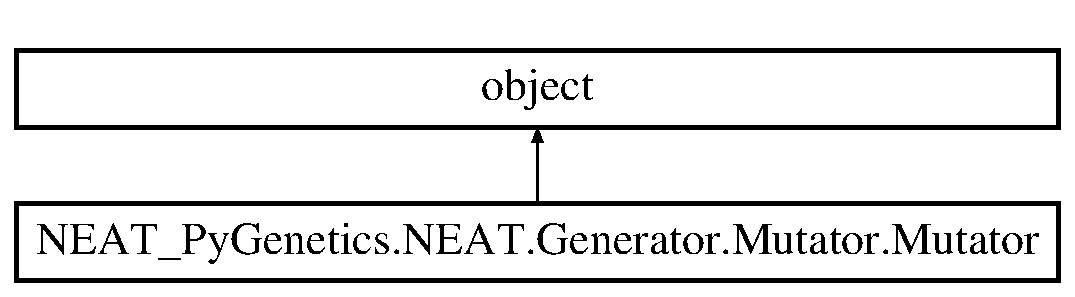
\includegraphics[height=2.000000cm]{classNEAT__PyGenetics_1_1NEAT_1_1Generator_1_1Mutator_1_1Mutator}
\end{center}
\end{figure}
\subsection*{Public Member Functions}
\begin{DoxyCompactItemize}
\item 
def \hyperlink{classNEAT__PyGenetics_1_1NEAT_1_1Generator_1_1Mutator_1_1Mutator_aef75e9ceb50c5d6df86ab49132a1fe84}{\+\_\+\+\_\+init\+\_\+\+\_\+} (self, \hyperlink{classNEAT__PyGenetics_1_1NEAT_1_1Generator_1_1Mutator_1_1Mutator_afa98da8eee10b2a4e9c653238dbbbe2c}{gene\+\_\+repository}, \hyperlink{classNEAT__PyGenetics_1_1NEAT_1_1Generator_1_1Mutator_1_1Mutator_a3339255b05437da752358f068835bc26}{mutation\+\_\+parameters})
\item 
def \hyperlink{classNEAT__PyGenetics_1_1NEAT_1_1Generator_1_1Mutator_1_1Mutator_aa805f3b8374dcf45ab4406f48bf145d5}{mutate\+\_\+genome} (self, genome)
\item 
def \hyperlink{classNEAT__PyGenetics_1_1NEAT_1_1Generator_1_1Mutator_1_1Mutator_aaee3498341c20339761db1301af7f341}{mutate\+\_\+add\+\_\+edge}
\item 
def \hyperlink{classNEAT__PyGenetics_1_1NEAT_1_1Generator_1_1Mutator_1_1Mutator_afeabd93fc71a47574e11dd8ac86b1cc2}{mutate\+\_\+add\+\_\+node}
\item 
def \hyperlink{classNEAT__PyGenetics_1_1NEAT_1_1Generator_1_1Mutator_1_1Mutator_aecb97c840811304711e07fe159b0c4bd}{mutate\+\_\+perturb\+\_\+weights}
\end{DoxyCompactItemize}
\subsection*{Static Public Member Functions}
\begin{DoxyCompactItemize}
\item 
def \hyperlink{classNEAT__PyGenetics_1_1NEAT_1_1Generator_1_1Mutator_1_1Mutator_ae8e05c9ff54df03a83a0809a7ba1f00a}{perturb\+\_\+weight}
\end{DoxyCompactItemize}
\subsection*{Public Attributes}
\begin{DoxyCompactItemize}
\item 
\hyperlink{classNEAT__PyGenetics_1_1NEAT_1_1Generator_1_1Mutator_1_1Mutator_afa98da8eee10b2a4e9c653238dbbbe2c}{gene\+\_\+repository}
\item 
\hyperlink{classNEAT__PyGenetics_1_1NEAT_1_1Generator_1_1Mutator_1_1Mutator_a3339255b05437da752358f068835bc26}{mutation\+\_\+parameters}
\end{DoxyCompactItemize}
\subsection*{Static Public Attributes}
\begin{DoxyCompactItemize}
\item 
\hyperlink{classNEAT__PyGenetics_1_1NEAT_1_1Generator_1_1Mutator_1_1Mutator_a74faa3a8d9acd9c1c0a68e145441fc5b}{starting\+\_\+vertex}
\item 
\hyperlink{classNEAT__PyGenetics_1_1NEAT_1_1Generator_1_1Mutator_1_1Mutator_add17af09898bf2a4203fed77bc404161}{possible\+\_\+endpoints}
\item 
\hyperlink{classNEAT__PyGenetics_1_1NEAT_1_1Generator_1_1Mutator_1_1Mutator_a7f7f636e283125c144a7781a6ac5afaa}{endpoint}
\item 
\hyperlink{classNEAT__PyGenetics_1_1NEAT_1_1Generator_1_1Mutator_1_1Mutator_a6479cbdd1acaed28cbdbdbc6d663ec89}{gene\+\_\+id}
\item 
\hyperlink{classNEAT__PyGenetics_1_1NEAT_1_1Generator_1_1Mutator_1_1Mutator_a85333a494bf1858ec78e1a304c5c25ec}{gene\+\_\+weight}
\item 
\hyperlink{classNEAT__PyGenetics_1_1NEAT_1_1Generator_1_1Mutator_1_1Mutator_a231e7983bed77578ecaa3d9b1d13e037}{gene\+\_\+enabled}
\item 
\hyperlink{classNEAT__PyGenetics_1_1NEAT_1_1Generator_1_1Mutator_1_1Mutator_a738d393eb3669111cf0fda1485019ca3}{new\+\_\+genome}
\item 
\hyperlink{classNEAT__PyGenetics_1_1NEAT_1_1Generator_1_1Mutator_1_1Mutator_a65fc450affae2ea20311a30dc4fb69af}{old\+\_\+gene\+\_\+id}
\item 
\hyperlink{classNEAT__PyGenetics_1_1NEAT_1_1Generator_1_1Mutator_1_1Mutator_a0dfab1f6afdafcbcb3f907471b66d588}{old\+\_\+gene}
\item 
\hyperlink{classNEAT__PyGenetics_1_1NEAT_1_1Generator_1_1Mutator_1_1Mutator_a2b1d1d4ca57366264f0e1648c575023f}{connecting\+\_\+nodes}
\item 
\hyperlink{classNEAT__PyGenetics_1_1NEAT_1_1Generator_1_1Mutator_1_1Mutator_aeaff4debf91f61a735965c3533ae1e6c}{connecting\+\_\+node}
\item 
\hyperlink{classNEAT__PyGenetics_1_1NEAT_1_1Generator_1_1Mutator_1_1Mutator_a346f32875edc5cb74b3d3555eaea80f9}{new\+\_\+gene\+\_\+one\+\_\+id}
\item 
\hyperlink{classNEAT__PyGenetics_1_1NEAT_1_1Generator_1_1Mutator_1_1Mutator_a77e03377943c33be52a1da66028c9386}{new\+\_\+gene\+\_\+one\+\_\+weight}
\item 
\hyperlink{classNEAT__PyGenetics_1_1NEAT_1_1Generator_1_1Mutator_1_1Mutator_a18e697e12c153b9679c214f9737f5f9c}{new\+\_\+gene\+\_\+one}
\item 
\hyperlink{classNEAT__PyGenetics_1_1NEAT_1_1Generator_1_1Mutator_1_1Mutator_a3fcf4df1bdecbc52e92ae8f63d38d473}{new\+\_\+gene\+\_\+two\+\_\+id}
\item 
\hyperlink{classNEAT__PyGenetics_1_1NEAT_1_1Generator_1_1Mutator_1_1Mutator_a3380ad2d05e8eace2063d8f1791274e0}{new\+\_\+gene\+\_\+two}
\item 
\hyperlink{classNEAT__PyGenetics_1_1NEAT_1_1Generator_1_1Mutator_1_1Mutator_a21e659d59a5f4ac929795dc4f5036f44}{new\+\_\+weight}
\end{DoxyCompactItemize}


\subsection{Constructor \& Destructor Documentation}
\index{N\+E\+A\+T\+\_\+\+Py\+Genetics\+::\+N\+E\+A\+T\+::\+Generator\+::\+Mutator\+::\+Mutator@{N\+E\+A\+T\+\_\+\+Py\+Genetics\+::\+N\+E\+A\+T\+::\+Generator\+::\+Mutator\+::\+Mutator}!\+\_\+\+\_\+init\+\_\+\+\_\+@{\+\_\+\+\_\+init\+\_\+\+\_\+}}
\index{\+\_\+\+\_\+init\+\_\+\+\_\+@{\+\_\+\+\_\+init\+\_\+\+\_\+}!N\+E\+A\+T\+\_\+\+Py\+Genetics\+::\+N\+E\+A\+T\+::\+Generator\+::\+Mutator\+::\+Mutator@{N\+E\+A\+T\+\_\+\+Py\+Genetics\+::\+N\+E\+A\+T\+::\+Generator\+::\+Mutator\+::\+Mutator}}
\subsubsection[{\texorpdfstring{\+\_\+\+\_\+init\+\_\+\+\_\+(self, gene\+\_\+repository, mutation\+\_\+parameters)}{__init__(self, gene_repository, mutation_parameters)}}]{\setlength{\rightskip}{0pt plus 5cm}def N\+E\+A\+T\+\_\+\+Py\+Genetics.\+N\+E\+A\+T.\+Generator.\+Mutator.\+Mutator.\+\_\+\+\_\+init\+\_\+\+\_\+ (
\begin{DoxyParamCaption}
\item[{}]{self, }
\item[{}]{gene\+\_\+repository, }
\item[{}]{mutation\+\_\+parameters}
\end{DoxyParamCaption}
)}\hypertarget{classNEAT__PyGenetics_1_1NEAT_1_1Generator_1_1Mutator_1_1Mutator_aef75e9ceb50c5d6df86ab49132a1fe84}{}\label{classNEAT__PyGenetics_1_1NEAT_1_1Generator_1_1Mutator_1_1Mutator_aef75e9ceb50c5d6df86ab49132a1fe84}


\subsection{Member Function Documentation}
\index{N\+E\+A\+T\+\_\+\+Py\+Genetics\+::\+N\+E\+A\+T\+::\+Generator\+::\+Mutator\+::\+Mutator@{N\+E\+A\+T\+\_\+\+Py\+Genetics\+::\+N\+E\+A\+T\+::\+Generator\+::\+Mutator\+::\+Mutator}!mutate\+\_\+add\+\_\+edge@{mutate\+\_\+add\+\_\+edge}}
\index{mutate\+\_\+add\+\_\+edge@{mutate\+\_\+add\+\_\+edge}!N\+E\+A\+T\+\_\+\+Py\+Genetics\+::\+N\+E\+A\+T\+::\+Generator\+::\+Mutator\+::\+Mutator@{N\+E\+A\+T\+\_\+\+Py\+Genetics\+::\+N\+E\+A\+T\+::\+Generator\+::\+Mutator\+::\+Mutator}}
\subsubsection[{\texorpdfstring{mutate\+\_\+add\+\_\+edge}{mutate_add_edge}}]{\setlength{\rightskip}{0pt plus 5cm}def N\+E\+A\+T\+\_\+\+Py\+Genetics.\+N\+E\+A\+T.\+Generator.\+Mutator.\+Mutator.\+mutate\+\_\+add\+\_\+edge (
\begin{DoxyParamCaption}
\item[{}]{self, }
\item[{}]{analysis\+\_\+genome}
\end{DoxyParamCaption}
)}\hypertarget{classNEAT__PyGenetics_1_1NEAT_1_1Generator_1_1Mutator_1_1Mutator_aaee3498341c20339761db1301af7f341}{}\label{classNEAT__PyGenetics_1_1NEAT_1_1Generator_1_1Mutator_1_1Mutator_aaee3498341c20339761db1301af7f341}
\index{N\+E\+A\+T\+\_\+\+Py\+Genetics\+::\+N\+E\+A\+T\+::\+Generator\+::\+Mutator\+::\+Mutator@{N\+E\+A\+T\+\_\+\+Py\+Genetics\+::\+N\+E\+A\+T\+::\+Generator\+::\+Mutator\+::\+Mutator}!mutate\+\_\+add\+\_\+node@{mutate\+\_\+add\+\_\+node}}
\index{mutate\+\_\+add\+\_\+node@{mutate\+\_\+add\+\_\+node}!N\+E\+A\+T\+\_\+\+Py\+Genetics\+::\+N\+E\+A\+T\+::\+Generator\+::\+Mutator\+::\+Mutator@{N\+E\+A\+T\+\_\+\+Py\+Genetics\+::\+N\+E\+A\+T\+::\+Generator\+::\+Mutator\+::\+Mutator}}
\subsubsection[{\texorpdfstring{mutate\+\_\+add\+\_\+node}{mutate_add_node}}]{\setlength{\rightskip}{0pt plus 5cm}def N\+E\+A\+T\+\_\+\+Py\+Genetics.\+N\+E\+A\+T.\+Generator.\+Mutator.\+Mutator.\+mutate\+\_\+add\+\_\+node (
\begin{DoxyParamCaption}
\item[{}]{self, }
\item[{}]{analysis\+\_\+genome}
\end{DoxyParamCaption}
)}\hypertarget{classNEAT__PyGenetics_1_1NEAT_1_1Generator_1_1Mutator_1_1Mutator_afeabd93fc71a47574e11dd8ac86b1cc2}{}\label{classNEAT__PyGenetics_1_1NEAT_1_1Generator_1_1Mutator_1_1Mutator_afeabd93fc71a47574e11dd8ac86b1cc2}
\index{N\+E\+A\+T\+\_\+\+Py\+Genetics\+::\+N\+E\+A\+T\+::\+Generator\+::\+Mutator\+::\+Mutator@{N\+E\+A\+T\+\_\+\+Py\+Genetics\+::\+N\+E\+A\+T\+::\+Generator\+::\+Mutator\+::\+Mutator}!mutate\+\_\+genome@{mutate\+\_\+genome}}
\index{mutate\+\_\+genome@{mutate\+\_\+genome}!N\+E\+A\+T\+\_\+\+Py\+Genetics\+::\+N\+E\+A\+T\+::\+Generator\+::\+Mutator\+::\+Mutator@{N\+E\+A\+T\+\_\+\+Py\+Genetics\+::\+N\+E\+A\+T\+::\+Generator\+::\+Mutator\+::\+Mutator}}
\subsubsection[{\texorpdfstring{mutate\+\_\+genome(self, genome)}{mutate_genome(self, genome)}}]{\setlength{\rightskip}{0pt plus 5cm}def N\+E\+A\+T\+\_\+\+Py\+Genetics.\+N\+E\+A\+T.\+Generator.\+Mutator.\+Mutator.\+mutate\+\_\+genome (
\begin{DoxyParamCaption}
\item[{}]{self, }
\item[{}]{genome, }
\item[{}]{Storage\+Genome}
\end{DoxyParamCaption}
)}\hypertarget{classNEAT__PyGenetics_1_1NEAT_1_1Generator_1_1Mutator_1_1Mutator_aa805f3b8374dcf45ab4406f48bf145d5}{}\label{classNEAT__PyGenetics_1_1NEAT_1_1Generator_1_1Mutator_1_1Mutator_aa805f3b8374dcf45ab4406f48bf145d5}
\index{N\+E\+A\+T\+\_\+\+Py\+Genetics\+::\+N\+E\+A\+T\+::\+Generator\+::\+Mutator\+::\+Mutator@{N\+E\+A\+T\+\_\+\+Py\+Genetics\+::\+N\+E\+A\+T\+::\+Generator\+::\+Mutator\+::\+Mutator}!mutate\+\_\+perturb\+\_\+weights@{mutate\+\_\+perturb\+\_\+weights}}
\index{mutate\+\_\+perturb\+\_\+weights@{mutate\+\_\+perturb\+\_\+weights}!N\+E\+A\+T\+\_\+\+Py\+Genetics\+::\+N\+E\+A\+T\+::\+Generator\+::\+Mutator\+::\+Mutator@{N\+E\+A\+T\+\_\+\+Py\+Genetics\+::\+N\+E\+A\+T\+::\+Generator\+::\+Mutator\+::\+Mutator}}
\subsubsection[{\texorpdfstring{mutate\+\_\+perturb\+\_\+weights}{mutate_perturb_weights}}]{\setlength{\rightskip}{0pt plus 5cm}def N\+E\+A\+T\+\_\+\+Py\+Genetics.\+N\+E\+A\+T.\+Generator.\+Mutator.\+Mutator.\+mutate\+\_\+perturb\+\_\+weights (
\begin{DoxyParamCaption}
\item[{}]{self, }
\item[{}]{genome}
\end{DoxyParamCaption}
)}\hypertarget{classNEAT__PyGenetics_1_1NEAT_1_1Generator_1_1Mutator_1_1Mutator_aecb97c840811304711e07fe159b0c4bd}{}\label{classNEAT__PyGenetics_1_1NEAT_1_1Generator_1_1Mutator_1_1Mutator_aecb97c840811304711e07fe159b0c4bd}
\index{N\+E\+A\+T\+\_\+\+Py\+Genetics\+::\+N\+E\+A\+T\+::\+Generator\+::\+Mutator\+::\+Mutator@{N\+E\+A\+T\+\_\+\+Py\+Genetics\+::\+N\+E\+A\+T\+::\+Generator\+::\+Mutator\+::\+Mutator}!perturb\+\_\+weight@{perturb\+\_\+weight}}
\index{perturb\+\_\+weight@{perturb\+\_\+weight}!N\+E\+A\+T\+\_\+\+Py\+Genetics\+::\+N\+E\+A\+T\+::\+Generator\+::\+Mutator\+::\+Mutator@{N\+E\+A\+T\+\_\+\+Py\+Genetics\+::\+N\+E\+A\+T\+::\+Generator\+::\+Mutator\+::\+Mutator}}
\subsubsection[{\texorpdfstring{perturb\+\_\+weight}{perturb_weight}}]{\setlength{\rightskip}{0pt plus 5cm}def N\+E\+A\+T\+\_\+\+Py\+Genetics.\+N\+E\+A\+T.\+Generator.\+Mutator.\+Mutator.\+perturb\+\_\+weight (
\begin{DoxyParamCaption}
\item[{}]{gene}
\end{DoxyParamCaption}
)\hspace{0.3cm}{\ttfamily [static]}}\hypertarget{classNEAT__PyGenetics_1_1NEAT_1_1Generator_1_1Mutator_1_1Mutator_ae8e05c9ff54df03a83a0809a7ba1f00a}{}\label{classNEAT__PyGenetics_1_1NEAT_1_1Generator_1_1Mutator_1_1Mutator_ae8e05c9ff54df03a83a0809a7ba1f00a}


\subsection{Member Data Documentation}
\index{N\+E\+A\+T\+\_\+\+Py\+Genetics\+::\+N\+E\+A\+T\+::\+Generator\+::\+Mutator\+::\+Mutator@{N\+E\+A\+T\+\_\+\+Py\+Genetics\+::\+N\+E\+A\+T\+::\+Generator\+::\+Mutator\+::\+Mutator}!connecting\+\_\+node@{connecting\+\_\+node}}
\index{connecting\+\_\+node@{connecting\+\_\+node}!N\+E\+A\+T\+\_\+\+Py\+Genetics\+::\+N\+E\+A\+T\+::\+Generator\+::\+Mutator\+::\+Mutator@{N\+E\+A\+T\+\_\+\+Py\+Genetics\+::\+N\+E\+A\+T\+::\+Generator\+::\+Mutator\+::\+Mutator}}
\subsubsection[{\texorpdfstring{connecting\+\_\+node}{connecting_node}}]{\setlength{\rightskip}{0pt plus 5cm}N\+E\+A\+T\+\_\+\+Py\+Genetics.\+N\+E\+A\+T.\+Generator.\+Mutator.\+Mutator.\+connecting\+\_\+node\hspace{0.3cm}{\ttfamily [static]}}\hypertarget{classNEAT__PyGenetics_1_1NEAT_1_1Generator_1_1Mutator_1_1Mutator_aeaff4debf91f61a735965c3533ae1e6c}{}\label{classNEAT__PyGenetics_1_1NEAT_1_1Generator_1_1Mutator_1_1Mutator_aeaff4debf91f61a735965c3533ae1e6c}
\index{N\+E\+A\+T\+\_\+\+Py\+Genetics\+::\+N\+E\+A\+T\+::\+Generator\+::\+Mutator\+::\+Mutator@{N\+E\+A\+T\+\_\+\+Py\+Genetics\+::\+N\+E\+A\+T\+::\+Generator\+::\+Mutator\+::\+Mutator}!connecting\+\_\+nodes@{connecting\+\_\+nodes}}
\index{connecting\+\_\+nodes@{connecting\+\_\+nodes}!N\+E\+A\+T\+\_\+\+Py\+Genetics\+::\+N\+E\+A\+T\+::\+Generator\+::\+Mutator\+::\+Mutator@{N\+E\+A\+T\+\_\+\+Py\+Genetics\+::\+N\+E\+A\+T\+::\+Generator\+::\+Mutator\+::\+Mutator}}
\subsubsection[{\texorpdfstring{connecting\+\_\+nodes}{connecting_nodes}}]{\setlength{\rightskip}{0pt plus 5cm}N\+E\+A\+T\+\_\+\+Py\+Genetics.\+N\+E\+A\+T.\+Generator.\+Mutator.\+Mutator.\+connecting\+\_\+nodes\hspace{0.3cm}{\ttfamily [static]}}\hypertarget{classNEAT__PyGenetics_1_1NEAT_1_1Generator_1_1Mutator_1_1Mutator_a2b1d1d4ca57366264f0e1648c575023f}{}\label{classNEAT__PyGenetics_1_1NEAT_1_1Generator_1_1Mutator_1_1Mutator_a2b1d1d4ca57366264f0e1648c575023f}
\index{N\+E\+A\+T\+\_\+\+Py\+Genetics\+::\+N\+E\+A\+T\+::\+Generator\+::\+Mutator\+::\+Mutator@{N\+E\+A\+T\+\_\+\+Py\+Genetics\+::\+N\+E\+A\+T\+::\+Generator\+::\+Mutator\+::\+Mutator}!endpoint@{endpoint}}
\index{endpoint@{endpoint}!N\+E\+A\+T\+\_\+\+Py\+Genetics\+::\+N\+E\+A\+T\+::\+Generator\+::\+Mutator\+::\+Mutator@{N\+E\+A\+T\+\_\+\+Py\+Genetics\+::\+N\+E\+A\+T\+::\+Generator\+::\+Mutator\+::\+Mutator}}
\subsubsection[{\texorpdfstring{endpoint}{endpoint}}]{\setlength{\rightskip}{0pt plus 5cm}N\+E\+A\+T\+\_\+\+Py\+Genetics.\+N\+E\+A\+T.\+Generator.\+Mutator.\+Mutator.\+endpoint\hspace{0.3cm}{\ttfamily [static]}}\hypertarget{classNEAT__PyGenetics_1_1NEAT_1_1Generator_1_1Mutator_1_1Mutator_a7f7f636e283125c144a7781a6ac5afaa}{}\label{classNEAT__PyGenetics_1_1NEAT_1_1Generator_1_1Mutator_1_1Mutator_a7f7f636e283125c144a7781a6ac5afaa}
\index{N\+E\+A\+T\+\_\+\+Py\+Genetics\+::\+N\+E\+A\+T\+::\+Generator\+::\+Mutator\+::\+Mutator@{N\+E\+A\+T\+\_\+\+Py\+Genetics\+::\+N\+E\+A\+T\+::\+Generator\+::\+Mutator\+::\+Mutator}!gene\+\_\+enabled@{gene\+\_\+enabled}}
\index{gene\+\_\+enabled@{gene\+\_\+enabled}!N\+E\+A\+T\+\_\+\+Py\+Genetics\+::\+N\+E\+A\+T\+::\+Generator\+::\+Mutator\+::\+Mutator@{N\+E\+A\+T\+\_\+\+Py\+Genetics\+::\+N\+E\+A\+T\+::\+Generator\+::\+Mutator\+::\+Mutator}}
\subsubsection[{\texorpdfstring{gene\+\_\+enabled}{gene_enabled}}]{\setlength{\rightskip}{0pt plus 5cm}N\+E\+A\+T\+\_\+\+Py\+Genetics.\+N\+E\+A\+T.\+Generator.\+Mutator.\+Mutator.\+gene\+\_\+enabled\hspace{0.3cm}{\ttfamily [static]}}\hypertarget{classNEAT__PyGenetics_1_1NEAT_1_1Generator_1_1Mutator_1_1Mutator_a231e7983bed77578ecaa3d9b1d13e037}{}\label{classNEAT__PyGenetics_1_1NEAT_1_1Generator_1_1Mutator_1_1Mutator_a231e7983bed77578ecaa3d9b1d13e037}
\index{N\+E\+A\+T\+\_\+\+Py\+Genetics\+::\+N\+E\+A\+T\+::\+Generator\+::\+Mutator\+::\+Mutator@{N\+E\+A\+T\+\_\+\+Py\+Genetics\+::\+N\+E\+A\+T\+::\+Generator\+::\+Mutator\+::\+Mutator}!gene\+\_\+id@{gene\+\_\+id}}
\index{gene\+\_\+id@{gene\+\_\+id}!N\+E\+A\+T\+\_\+\+Py\+Genetics\+::\+N\+E\+A\+T\+::\+Generator\+::\+Mutator\+::\+Mutator@{N\+E\+A\+T\+\_\+\+Py\+Genetics\+::\+N\+E\+A\+T\+::\+Generator\+::\+Mutator\+::\+Mutator}}
\subsubsection[{\texorpdfstring{gene\+\_\+id}{gene_id}}]{\setlength{\rightskip}{0pt plus 5cm}N\+E\+A\+T\+\_\+\+Py\+Genetics.\+N\+E\+A\+T.\+Generator.\+Mutator.\+Mutator.\+gene\+\_\+id\hspace{0.3cm}{\ttfamily [static]}}\hypertarget{classNEAT__PyGenetics_1_1NEAT_1_1Generator_1_1Mutator_1_1Mutator_a6479cbdd1acaed28cbdbdbc6d663ec89}{}\label{classNEAT__PyGenetics_1_1NEAT_1_1Generator_1_1Mutator_1_1Mutator_a6479cbdd1acaed28cbdbdbc6d663ec89}
\index{N\+E\+A\+T\+\_\+\+Py\+Genetics\+::\+N\+E\+A\+T\+::\+Generator\+::\+Mutator\+::\+Mutator@{N\+E\+A\+T\+\_\+\+Py\+Genetics\+::\+N\+E\+A\+T\+::\+Generator\+::\+Mutator\+::\+Mutator}!gene\+\_\+repository@{gene\+\_\+repository}}
\index{gene\+\_\+repository@{gene\+\_\+repository}!N\+E\+A\+T\+\_\+\+Py\+Genetics\+::\+N\+E\+A\+T\+::\+Generator\+::\+Mutator\+::\+Mutator@{N\+E\+A\+T\+\_\+\+Py\+Genetics\+::\+N\+E\+A\+T\+::\+Generator\+::\+Mutator\+::\+Mutator}}
\subsubsection[{\texorpdfstring{gene\+\_\+repository}{gene_repository}}]{\setlength{\rightskip}{0pt plus 5cm}N\+E\+A\+T\+\_\+\+Py\+Genetics.\+N\+E\+A\+T.\+Generator.\+Mutator.\+Mutator.\+gene\+\_\+repository}\hypertarget{classNEAT__PyGenetics_1_1NEAT_1_1Generator_1_1Mutator_1_1Mutator_afa98da8eee10b2a4e9c653238dbbbe2c}{}\label{classNEAT__PyGenetics_1_1NEAT_1_1Generator_1_1Mutator_1_1Mutator_afa98da8eee10b2a4e9c653238dbbbe2c}
\index{N\+E\+A\+T\+\_\+\+Py\+Genetics\+::\+N\+E\+A\+T\+::\+Generator\+::\+Mutator\+::\+Mutator@{N\+E\+A\+T\+\_\+\+Py\+Genetics\+::\+N\+E\+A\+T\+::\+Generator\+::\+Mutator\+::\+Mutator}!gene\+\_\+weight@{gene\+\_\+weight}}
\index{gene\+\_\+weight@{gene\+\_\+weight}!N\+E\+A\+T\+\_\+\+Py\+Genetics\+::\+N\+E\+A\+T\+::\+Generator\+::\+Mutator\+::\+Mutator@{N\+E\+A\+T\+\_\+\+Py\+Genetics\+::\+N\+E\+A\+T\+::\+Generator\+::\+Mutator\+::\+Mutator}}
\subsubsection[{\texorpdfstring{gene\+\_\+weight}{gene_weight}}]{\setlength{\rightskip}{0pt plus 5cm}N\+E\+A\+T\+\_\+\+Py\+Genetics.\+N\+E\+A\+T.\+Generator.\+Mutator.\+Mutator.\+gene\+\_\+weight\hspace{0.3cm}{\ttfamily [static]}}\hypertarget{classNEAT__PyGenetics_1_1NEAT_1_1Generator_1_1Mutator_1_1Mutator_a85333a494bf1858ec78e1a304c5c25ec}{}\label{classNEAT__PyGenetics_1_1NEAT_1_1Generator_1_1Mutator_1_1Mutator_a85333a494bf1858ec78e1a304c5c25ec}
\index{N\+E\+A\+T\+\_\+\+Py\+Genetics\+::\+N\+E\+A\+T\+::\+Generator\+::\+Mutator\+::\+Mutator@{N\+E\+A\+T\+\_\+\+Py\+Genetics\+::\+N\+E\+A\+T\+::\+Generator\+::\+Mutator\+::\+Mutator}!mutation\+\_\+parameters@{mutation\+\_\+parameters}}
\index{mutation\+\_\+parameters@{mutation\+\_\+parameters}!N\+E\+A\+T\+\_\+\+Py\+Genetics\+::\+N\+E\+A\+T\+::\+Generator\+::\+Mutator\+::\+Mutator@{N\+E\+A\+T\+\_\+\+Py\+Genetics\+::\+N\+E\+A\+T\+::\+Generator\+::\+Mutator\+::\+Mutator}}
\subsubsection[{\texorpdfstring{mutation\+\_\+parameters}{mutation_parameters}}]{\setlength{\rightskip}{0pt plus 5cm}N\+E\+A\+T\+\_\+\+Py\+Genetics.\+N\+E\+A\+T.\+Generator.\+Mutator.\+Mutator.\+mutation\+\_\+parameters}\hypertarget{classNEAT__PyGenetics_1_1NEAT_1_1Generator_1_1Mutator_1_1Mutator_a3339255b05437da752358f068835bc26}{}\label{classNEAT__PyGenetics_1_1NEAT_1_1Generator_1_1Mutator_1_1Mutator_a3339255b05437da752358f068835bc26}
\index{N\+E\+A\+T\+\_\+\+Py\+Genetics\+::\+N\+E\+A\+T\+::\+Generator\+::\+Mutator\+::\+Mutator@{N\+E\+A\+T\+\_\+\+Py\+Genetics\+::\+N\+E\+A\+T\+::\+Generator\+::\+Mutator\+::\+Mutator}!new\+\_\+gene\+\_\+one@{new\+\_\+gene\+\_\+one}}
\index{new\+\_\+gene\+\_\+one@{new\+\_\+gene\+\_\+one}!N\+E\+A\+T\+\_\+\+Py\+Genetics\+::\+N\+E\+A\+T\+::\+Generator\+::\+Mutator\+::\+Mutator@{N\+E\+A\+T\+\_\+\+Py\+Genetics\+::\+N\+E\+A\+T\+::\+Generator\+::\+Mutator\+::\+Mutator}}
\subsubsection[{\texorpdfstring{new\+\_\+gene\+\_\+one}{new_gene_one}}]{\setlength{\rightskip}{0pt plus 5cm}N\+E\+A\+T\+\_\+\+Py\+Genetics.\+N\+E\+A\+T.\+Generator.\+Mutator.\+Mutator.\+new\+\_\+gene\+\_\+one\hspace{0.3cm}{\ttfamily [static]}}\hypertarget{classNEAT__PyGenetics_1_1NEAT_1_1Generator_1_1Mutator_1_1Mutator_a18e697e12c153b9679c214f9737f5f9c}{}\label{classNEAT__PyGenetics_1_1NEAT_1_1Generator_1_1Mutator_1_1Mutator_a18e697e12c153b9679c214f9737f5f9c}
\index{N\+E\+A\+T\+\_\+\+Py\+Genetics\+::\+N\+E\+A\+T\+::\+Generator\+::\+Mutator\+::\+Mutator@{N\+E\+A\+T\+\_\+\+Py\+Genetics\+::\+N\+E\+A\+T\+::\+Generator\+::\+Mutator\+::\+Mutator}!new\+\_\+gene\+\_\+one\+\_\+id@{new\+\_\+gene\+\_\+one\+\_\+id}}
\index{new\+\_\+gene\+\_\+one\+\_\+id@{new\+\_\+gene\+\_\+one\+\_\+id}!N\+E\+A\+T\+\_\+\+Py\+Genetics\+::\+N\+E\+A\+T\+::\+Generator\+::\+Mutator\+::\+Mutator@{N\+E\+A\+T\+\_\+\+Py\+Genetics\+::\+N\+E\+A\+T\+::\+Generator\+::\+Mutator\+::\+Mutator}}
\subsubsection[{\texorpdfstring{new\+\_\+gene\+\_\+one\+\_\+id}{new_gene_one_id}}]{\setlength{\rightskip}{0pt plus 5cm}N\+E\+A\+T\+\_\+\+Py\+Genetics.\+N\+E\+A\+T.\+Generator.\+Mutator.\+Mutator.\+new\+\_\+gene\+\_\+one\+\_\+id\hspace{0.3cm}{\ttfamily [static]}}\hypertarget{classNEAT__PyGenetics_1_1NEAT_1_1Generator_1_1Mutator_1_1Mutator_a346f32875edc5cb74b3d3555eaea80f9}{}\label{classNEAT__PyGenetics_1_1NEAT_1_1Generator_1_1Mutator_1_1Mutator_a346f32875edc5cb74b3d3555eaea80f9}
\index{N\+E\+A\+T\+\_\+\+Py\+Genetics\+::\+N\+E\+A\+T\+::\+Generator\+::\+Mutator\+::\+Mutator@{N\+E\+A\+T\+\_\+\+Py\+Genetics\+::\+N\+E\+A\+T\+::\+Generator\+::\+Mutator\+::\+Mutator}!new\+\_\+gene\+\_\+one\+\_\+weight@{new\+\_\+gene\+\_\+one\+\_\+weight}}
\index{new\+\_\+gene\+\_\+one\+\_\+weight@{new\+\_\+gene\+\_\+one\+\_\+weight}!N\+E\+A\+T\+\_\+\+Py\+Genetics\+::\+N\+E\+A\+T\+::\+Generator\+::\+Mutator\+::\+Mutator@{N\+E\+A\+T\+\_\+\+Py\+Genetics\+::\+N\+E\+A\+T\+::\+Generator\+::\+Mutator\+::\+Mutator}}
\subsubsection[{\texorpdfstring{new\+\_\+gene\+\_\+one\+\_\+weight}{new_gene_one_weight}}]{\setlength{\rightskip}{0pt plus 5cm}N\+E\+A\+T\+\_\+\+Py\+Genetics.\+N\+E\+A\+T.\+Generator.\+Mutator.\+Mutator.\+new\+\_\+gene\+\_\+one\+\_\+weight\hspace{0.3cm}{\ttfamily [static]}}\hypertarget{classNEAT__PyGenetics_1_1NEAT_1_1Generator_1_1Mutator_1_1Mutator_a77e03377943c33be52a1da66028c9386}{}\label{classNEAT__PyGenetics_1_1NEAT_1_1Generator_1_1Mutator_1_1Mutator_a77e03377943c33be52a1da66028c9386}
\index{N\+E\+A\+T\+\_\+\+Py\+Genetics\+::\+N\+E\+A\+T\+::\+Generator\+::\+Mutator\+::\+Mutator@{N\+E\+A\+T\+\_\+\+Py\+Genetics\+::\+N\+E\+A\+T\+::\+Generator\+::\+Mutator\+::\+Mutator}!new\+\_\+gene\+\_\+two@{new\+\_\+gene\+\_\+two}}
\index{new\+\_\+gene\+\_\+two@{new\+\_\+gene\+\_\+two}!N\+E\+A\+T\+\_\+\+Py\+Genetics\+::\+N\+E\+A\+T\+::\+Generator\+::\+Mutator\+::\+Mutator@{N\+E\+A\+T\+\_\+\+Py\+Genetics\+::\+N\+E\+A\+T\+::\+Generator\+::\+Mutator\+::\+Mutator}}
\subsubsection[{\texorpdfstring{new\+\_\+gene\+\_\+two}{new_gene_two}}]{\setlength{\rightskip}{0pt plus 5cm}N\+E\+A\+T\+\_\+\+Py\+Genetics.\+N\+E\+A\+T.\+Generator.\+Mutator.\+Mutator.\+new\+\_\+gene\+\_\+two\hspace{0.3cm}{\ttfamily [static]}}\hypertarget{classNEAT__PyGenetics_1_1NEAT_1_1Generator_1_1Mutator_1_1Mutator_a3380ad2d05e8eace2063d8f1791274e0}{}\label{classNEAT__PyGenetics_1_1NEAT_1_1Generator_1_1Mutator_1_1Mutator_a3380ad2d05e8eace2063d8f1791274e0}
\index{N\+E\+A\+T\+\_\+\+Py\+Genetics\+::\+N\+E\+A\+T\+::\+Generator\+::\+Mutator\+::\+Mutator@{N\+E\+A\+T\+\_\+\+Py\+Genetics\+::\+N\+E\+A\+T\+::\+Generator\+::\+Mutator\+::\+Mutator}!new\+\_\+gene\+\_\+two\+\_\+id@{new\+\_\+gene\+\_\+two\+\_\+id}}
\index{new\+\_\+gene\+\_\+two\+\_\+id@{new\+\_\+gene\+\_\+two\+\_\+id}!N\+E\+A\+T\+\_\+\+Py\+Genetics\+::\+N\+E\+A\+T\+::\+Generator\+::\+Mutator\+::\+Mutator@{N\+E\+A\+T\+\_\+\+Py\+Genetics\+::\+N\+E\+A\+T\+::\+Generator\+::\+Mutator\+::\+Mutator}}
\subsubsection[{\texorpdfstring{new\+\_\+gene\+\_\+two\+\_\+id}{new_gene_two_id}}]{\setlength{\rightskip}{0pt plus 5cm}N\+E\+A\+T\+\_\+\+Py\+Genetics.\+N\+E\+A\+T.\+Generator.\+Mutator.\+Mutator.\+new\+\_\+gene\+\_\+two\+\_\+id\hspace{0.3cm}{\ttfamily [static]}}\hypertarget{classNEAT__PyGenetics_1_1NEAT_1_1Generator_1_1Mutator_1_1Mutator_a3fcf4df1bdecbc52e92ae8f63d38d473}{}\label{classNEAT__PyGenetics_1_1NEAT_1_1Generator_1_1Mutator_1_1Mutator_a3fcf4df1bdecbc52e92ae8f63d38d473}
\index{N\+E\+A\+T\+\_\+\+Py\+Genetics\+::\+N\+E\+A\+T\+::\+Generator\+::\+Mutator\+::\+Mutator@{N\+E\+A\+T\+\_\+\+Py\+Genetics\+::\+N\+E\+A\+T\+::\+Generator\+::\+Mutator\+::\+Mutator}!new\+\_\+genome@{new\+\_\+genome}}
\index{new\+\_\+genome@{new\+\_\+genome}!N\+E\+A\+T\+\_\+\+Py\+Genetics\+::\+N\+E\+A\+T\+::\+Generator\+::\+Mutator\+::\+Mutator@{N\+E\+A\+T\+\_\+\+Py\+Genetics\+::\+N\+E\+A\+T\+::\+Generator\+::\+Mutator\+::\+Mutator}}
\subsubsection[{\texorpdfstring{new\+\_\+genome}{new_genome}}]{\setlength{\rightskip}{0pt plus 5cm}N\+E\+A\+T\+\_\+\+Py\+Genetics.\+N\+E\+A\+T.\+Generator.\+Mutator.\+Mutator.\+new\+\_\+genome\hspace{0.3cm}{\ttfamily [static]}}\hypertarget{classNEAT__PyGenetics_1_1NEAT_1_1Generator_1_1Mutator_1_1Mutator_a738d393eb3669111cf0fda1485019ca3}{}\label{classNEAT__PyGenetics_1_1NEAT_1_1Generator_1_1Mutator_1_1Mutator_a738d393eb3669111cf0fda1485019ca3}
\index{N\+E\+A\+T\+\_\+\+Py\+Genetics\+::\+N\+E\+A\+T\+::\+Generator\+::\+Mutator\+::\+Mutator@{N\+E\+A\+T\+\_\+\+Py\+Genetics\+::\+N\+E\+A\+T\+::\+Generator\+::\+Mutator\+::\+Mutator}!new\+\_\+weight@{new\+\_\+weight}}
\index{new\+\_\+weight@{new\+\_\+weight}!N\+E\+A\+T\+\_\+\+Py\+Genetics\+::\+N\+E\+A\+T\+::\+Generator\+::\+Mutator\+::\+Mutator@{N\+E\+A\+T\+\_\+\+Py\+Genetics\+::\+N\+E\+A\+T\+::\+Generator\+::\+Mutator\+::\+Mutator}}
\subsubsection[{\texorpdfstring{new\+\_\+weight}{new_weight}}]{\setlength{\rightskip}{0pt plus 5cm}N\+E\+A\+T\+\_\+\+Py\+Genetics.\+N\+E\+A\+T.\+Generator.\+Mutator.\+Mutator.\+new\+\_\+weight\hspace{0.3cm}{\ttfamily [static]}}\hypertarget{classNEAT__PyGenetics_1_1NEAT_1_1Generator_1_1Mutator_1_1Mutator_a21e659d59a5f4ac929795dc4f5036f44}{}\label{classNEAT__PyGenetics_1_1NEAT_1_1Generator_1_1Mutator_1_1Mutator_a21e659d59a5f4ac929795dc4f5036f44}
\index{N\+E\+A\+T\+\_\+\+Py\+Genetics\+::\+N\+E\+A\+T\+::\+Generator\+::\+Mutator\+::\+Mutator@{N\+E\+A\+T\+\_\+\+Py\+Genetics\+::\+N\+E\+A\+T\+::\+Generator\+::\+Mutator\+::\+Mutator}!old\+\_\+gene@{old\+\_\+gene}}
\index{old\+\_\+gene@{old\+\_\+gene}!N\+E\+A\+T\+\_\+\+Py\+Genetics\+::\+N\+E\+A\+T\+::\+Generator\+::\+Mutator\+::\+Mutator@{N\+E\+A\+T\+\_\+\+Py\+Genetics\+::\+N\+E\+A\+T\+::\+Generator\+::\+Mutator\+::\+Mutator}}
\subsubsection[{\texorpdfstring{old\+\_\+gene}{old_gene}}]{\setlength{\rightskip}{0pt plus 5cm}N\+E\+A\+T\+\_\+\+Py\+Genetics.\+N\+E\+A\+T.\+Generator.\+Mutator.\+Mutator.\+old\+\_\+gene\hspace{0.3cm}{\ttfamily [static]}}\hypertarget{classNEAT__PyGenetics_1_1NEAT_1_1Generator_1_1Mutator_1_1Mutator_a0dfab1f6afdafcbcb3f907471b66d588}{}\label{classNEAT__PyGenetics_1_1NEAT_1_1Generator_1_1Mutator_1_1Mutator_a0dfab1f6afdafcbcb3f907471b66d588}
\index{N\+E\+A\+T\+\_\+\+Py\+Genetics\+::\+N\+E\+A\+T\+::\+Generator\+::\+Mutator\+::\+Mutator@{N\+E\+A\+T\+\_\+\+Py\+Genetics\+::\+N\+E\+A\+T\+::\+Generator\+::\+Mutator\+::\+Mutator}!old\+\_\+gene\+\_\+id@{old\+\_\+gene\+\_\+id}}
\index{old\+\_\+gene\+\_\+id@{old\+\_\+gene\+\_\+id}!N\+E\+A\+T\+\_\+\+Py\+Genetics\+::\+N\+E\+A\+T\+::\+Generator\+::\+Mutator\+::\+Mutator@{N\+E\+A\+T\+\_\+\+Py\+Genetics\+::\+N\+E\+A\+T\+::\+Generator\+::\+Mutator\+::\+Mutator}}
\subsubsection[{\texorpdfstring{old\+\_\+gene\+\_\+id}{old_gene_id}}]{\setlength{\rightskip}{0pt plus 5cm}N\+E\+A\+T\+\_\+\+Py\+Genetics.\+N\+E\+A\+T.\+Generator.\+Mutator.\+Mutator.\+old\+\_\+gene\+\_\+id\hspace{0.3cm}{\ttfamily [static]}}\hypertarget{classNEAT__PyGenetics_1_1NEAT_1_1Generator_1_1Mutator_1_1Mutator_a65fc450affae2ea20311a30dc4fb69af}{}\label{classNEAT__PyGenetics_1_1NEAT_1_1Generator_1_1Mutator_1_1Mutator_a65fc450affae2ea20311a30dc4fb69af}
\index{N\+E\+A\+T\+\_\+\+Py\+Genetics\+::\+N\+E\+A\+T\+::\+Generator\+::\+Mutator\+::\+Mutator@{N\+E\+A\+T\+\_\+\+Py\+Genetics\+::\+N\+E\+A\+T\+::\+Generator\+::\+Mutator\+::\+Mutator}!possible\+\_\+endpoints@{possible\+\_\+endpoints}}
\index{possible\+\_\+endpoints@{possible\+\_\+endpoints}!N\+E\+A\+T\+\_\+\+Py\+Genetics\+::\+N\+E\+A\+T\+::\+Generator\+::\+Mutator\+::\+Mutator@{N\+E\+A\+T\+\_\+\+Py\+Genetics\+::\+N\+E\+A\+T\+::\+Generator\+::\+Mutator\+::\+Mutator}}
\subsubsection[{\texorpdfstring{possible\+\_\+endpoints}{possible_endpoints}}]{\setlength{\rightskip}{0pt plus 5cm}N\+E\+A\+T\+\_\+\+Py\+Genetics.\+N\+E\+A\+T.\+Generator.\+Mutator.\+Mutator.\+possible\+\_\+endpoints\hspace{0.3cm}{\ttfamily [static]}}\hypertarget{classNEAT__PyGenetics_1_1NEAT_1_1Generator_1_1Mutator_1_1Mutator_add17af09898bf2a4203fed77bc404161}{}\label{classNEAT__PyGenetics_1_1NEAT_1_1Generator_1_1Mutator_1_1Mutator_add17af09898bf2a4203fed77bc404161}
\index{N\+E\+A\+T\+\_\+\+Py\+Genetics\+::\+N\+E\+A\+T\+::\+Generator\+::\+Mutator\+::\+Mutator@{N\+E\+A\+T\+\_\+\+Py\+Genetics\+::\+N\+E\+A\+T\+::\+Generator\+::\+Mutator\+::\+Mutator}!starting\+\_\+vertex@{starting\+\_\+vertex}}
\index{starting\+\_\+vertex@{starting\+\_\+vertex}!N\+E\+A\+T\+\_\+\+Py\+Genetics\+::\+N\+E\+A\+T\+::\+Generator\+::\+Mutator\+::\+Mutator@{N\+E\+A\+T\+\_\+\+Py\+Genetics\+::\+N\+E\+A\+T\+::\+Generator\+::\+Mutator\+::\+Mutator}}
\subsubsection[{\texorpdfstring{starting\+\_\+vertex}{starting_vertex}}]{\setlength{\rightskip}{0pt plus 5cm}N\+E\+A\+T\+\_\+\+Py\+Genetics.\+N\+E\+A\+T.\+Generator.\+Mutator.\+Mutator.\+starting\+\_\+vertex\hspace{0.3cm}{\ttfamily [static]}}\hypertarget{classNEAT__PyGenetics_1_1NEAT_1_1Generator_1_1Mutator_1_1Mutator_a74faa3a8d9acd9c1c0a68e145441fc5b}{}\label{classNEAT__PyGenetics_1_1NEAT_1_1Generator_1_1Mutator_1_1Mutator_a74faa3a8d9acd9c1c0a68e145441fc5b}


The documentation for this class was generated from the following file\+:\begin{DoxyCompactItemize}
\item 
N\+E\+A\+T/\+Generator/\hyperlink{Mutator_8py}{Mutator.\+py}\end{DoxyCompactItemize}

\hypertarget{classNEAT__PyGenetics_1_1NEAT_1_1Networking_1_1Client_1_1NEATClient_1_1NEATClient}{}\section{N\+E\+A\+T\+\_\+\+Py\+Genetics.\+N\+E\+A\+T.\+Networking.\+Client.\+N\+E\+A\+T\+Client.\+N\+E\+A\+T\+Client Class Reference}
\label{classNEAT__PyGenetics_1_1NEAT_1_1Networking_1_1Client_1_1NEATClient_1_1NEATClient}\index{N\+E\+A\+T\+\_\+\+Py\+Genetics.\+N\+E\+A\+T.\+Networking.\+Client.\+N\+E\+A\+T\+Client.\+N\+E\+A\+T\+Client@{N\+E\+A\+T\+\_\+\+Py\+Genetics.\+N\+E\+A\+T.\+Networking.\+Client.\+N\+E\+A\+T\+Client.\+N\+E\+A\+T\+Client}}
Inheritance diagram for N\+E\+A\+T\+\_\+\+Py\+Genetics.\+N\+E\+A\+T.\+Networking.\+Client.\+N\+E\+A\+T\+Client.\+N\+E\+A\+T\+Client\+:\begin{figure}[H]
\begin{center}
\leavevmode
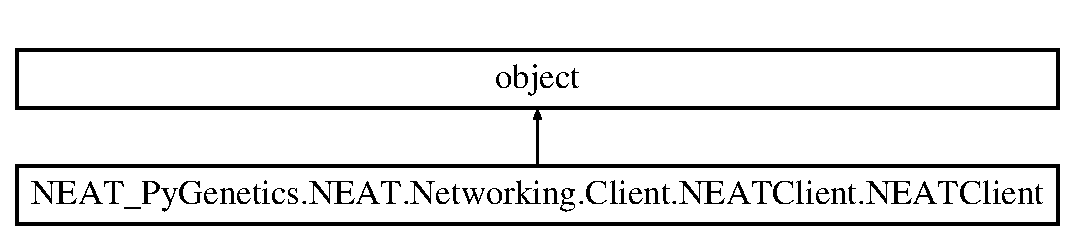
\includegraphics[height=2.000000cm]{classNEAT__PyGenetics_1_1NEAT_1_1Networking_1_1Client_1_1NEATClient_1_1NEATClient}
\end{center}
\end{figure}
\subsection*{Public Member Functions}
\begin{DoxyCompactItemize}
\item 
def \hyperlink{classNEAT__PyGenetics_1_1NEAT_1_1Networking_1_1Client_1_1NEATClient_1_1NEATClient_a9e84283e9dab07424cbbef8d966fd74b}{\+\_\+\+\_\+init\+\_\+\+\_\+} (self, server\+\_\+address, server\+\_\+port)
\item 
def \hyperlink{classNEAT__PyGenetics_1_1NEAT_1_1Networking_1_1Client_1_1NEATClient_1_1NEATClient_a58156abc06c16b0f2399219655c7321c}{run\+\_\+command} (self, command)
\end{DoxyCompactItemize}


\subsection{Constructor \& Destructor Documentation}
\index{N\+E\+A\+T\+\_\+\+Py\+Genetics\+::\+N\+E\+A\+T\+::\+Networking\+::\+Client\+::\+N\+E\+A\+T\+Client\+::\+N\+E\+A\+T\+Client@{N\+E\+A\+T\+\_\+\+Py\+Genetics\+::\+N\+E\+A\+T\+::\+Networking\+::\+Client\+::\+N\+E\+A\+T\+Client\+::\+N\+E\+A\+T\+Client}!\+\_\+\+\_\+init\+\_\+\+\_\+@{\+\_\+\+\_\+init\+\_\+\+\_\+}}
\index{\+\_\+\+\_\+init\+\_\+\+\_\+@{\+\_\+\+\_\+init\+\_\+\+\_\+}!N\+E\+A\+T\+\_\+\+Py\+Genetics\+::\+N\+E\+A\+T\+::\+Networking\+::\+Client\+::\+N\+E\+A\+T\+Client\+::\+N\+E\+A\+T\+Client@{N\+E\+A\+T\+\_\+\+Py\+Genetics\+::\+N\+E\+A\+T\+::\+Networking\+::\+Client\+::\+N\+E\+A\+T\+Client\+::\+N\+E\+A\+T\+Client}}
\subsubsection[{\texorpdfstring{\+\_\+\+\_\+init\+\_\+\+\_\+(self, server\+\_\+address, server\+\_\+port)}{__init__(self, server_address, server_port)}}]{\setlength{\rightskip}{0pt plus 5cm}def N\+E\+A\+T\+\_\+\+Py\+Genetics.\+N\+E\+A\+T.\+Networking.\+Client.\+N\+E\+A\+T\+Client.\+N\+E\+A\+T\+Client.\+\_\+\+\_\+init\+\_\+\+\_\+ (
\begin{DoxyParamCaption}
\item[{}]{self, }
\item[{}]{server\+\_\+address, }
\item[{}]{server\+\_\+port}
\end{DoxyParamCaption}
)}\hypertarget{classNEAT__PyGenetics_1_1NEAT_1_1Networking_1_1Client_1_1NEATClient_1_1NEATClient_a9e84283e9dab07424cbbef8d966fd74b}{}\label{classNEAT__PyGenetics_1_1NEAT_1_1Networking_1_1Client_1_1NEATClient_1_1NEATClient_a9e84283e9dab07424cbbef8d966fd74b}


\subsection{Member Function Documentation}
\index{N\+E\+A\+T\+\_\+\+Py\+Genetics\+::\+N\+E\+A\+T\+::\+Networking\+::\+Client\+::\+N\+E\+A\+T\+Client\+::\+N\+E\+A\+T\+Client@{N\+E\+A\+T\+\_\+\+Py\+Genetics\+::\+N\+E\+A\+T\+::\+Networking\+::\+Client\+::\+N\+E\+A\+T\+Client\+::\+N\+E\+A\+T\+Client}!run\+\_\+command@{run\+\_\+command}}
\index{run\+\_\+command@{run\+\_\+command}!N\+E\+A\+T\+\_\+\+Py\+Genetics\+::\+N\+E\+A\+T\+::\+Networking\+::\+Client\+::\+N\+E\+A\+T\+Client\+::\+N\+E\+A\+T\+Client@{N\+E\+A\+T\+\_\+\+Py\+Genetics\+::\+N\+E\+A\+T\+::\+Networking\+::\+Client\+::\+N\+E\+A\+T\+Client\+::\+N\+E\+A\+T\+Client}}
\subsubsection[{\texorpdfstring{run\+\_\+command(self, command)}{run_command(self, command)}}]{\setlength{\rightskip}{0pt plus 5cm}def N\+E\+A\+T\+\_\+\+Py\+Genetics.\+N\+E\+A\+T.\+Networking.\+Client.\+N\+E\+A\+T\+Client.\+N\+E\+A\+T\+Client.\+run\+\_\+command (
\begin{DoxyParamCaption}
\item[{}]{self, }
\item[{}]{command}
\end{DoxyParamCaption}
)}\hypertarget{classNEAT__PyGenetics_1_1NEAT_1_1Networking_1_1Client_1_1NEATClient_1_1NEATClient_a58156abc06c16b0f2399219655c7321c}{}\label{classNEAT__PyGenetics_1_1NEAT_1_1Networking_1_1Client_1_1NEATClient_1_1NEATClient_a58156abc06c16b0f2399219655c7321c}


The documentation for this class was generated from the following file\+:\begin{DoxyCompactItemize}
\item 
N\+E\+A\+T/\+Networking/\+Client/\hyperlink{NEATClient_8py}{N\+E\+A\+T\+Client.\+py}\end{DoxyCompactItemize}

\hypertarget{classNEAT__PyGenetics_1_1NEAT_1_1Config_1_1NEATConfig_1_1NEATConfig}{}\section{N\+E\+A\+T\+\_\+\+Py\+Genetics.\+N\+E\+A\+T.\+Config.\+N\+E\+A\+T\+Config.\+N\+E\+A\+T\+Config Class Reference}
\label{classNEAT__PyGenetics_1_1NEAT_1_1Config_1_1NEATConfig_1_1NEATConfig}\index{N\+E\+A\+T\+\_\+\+Py\+Genetics.\+N\+E\+A\+T.\+Config.\+N\+E\+A\+T\+Config.\+N\+E\+A\+T\+Config@{N\+E\+A\+T\+\_\+\+Py\+Genetics.\+N\+E\+A\+T.\+Config.\+N\+E\+A\+T\+Config.\+N\+E\+A\+T\+Config}}
Inheritance diagram for N\+E\+A\+T\+\_\+\+Py\+Genetics.\+N\+E\+A\+T.\+Config.\+N\+E\+A\+T\+Config.\+N\+E\+A\+T\+Config\+:\begin{figure}[H]
\begin{center}
\leavevmode
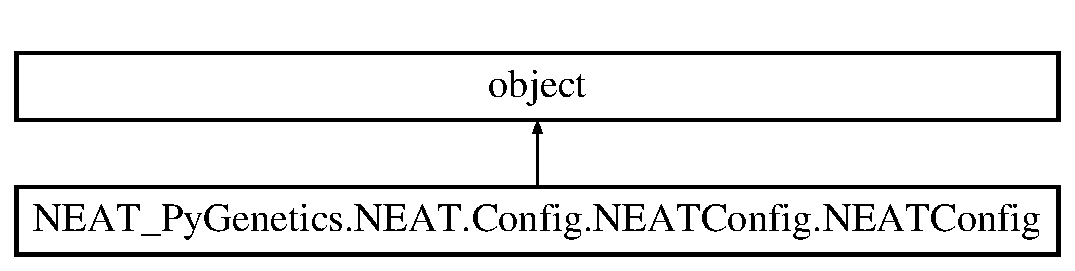
\includegraphics[height=2.000000cm]{classNEAT__PyGenetics_1_1NEAT_1_1Config_1_1NEATConfig_1_1NEATConfig}
\end{center}
\end{figure}
\subsection*{Public Member Functions}
\begin{DoxyCompactItemize}
\item 
def \hyperlink{classNEAT__PyGenetics_1_1NEAT_1_1Config_1_1NEATConfig_1_1NEATConfig_a88504e0a5c56f166a3ee5898ae3e0dea}{\+\_\+\+\_\+init\+\_\+\+\_\+} (self, config\+\_\+path=None)
\item 
def \hyperlink{classNEAT__PyGenetics_1_1NEAT_1_1Config_1_1NEATConfig_1_1NEATConfig_aa6843226e3a017a384c8244f4e62e0f5}{load\+\_\+config} (self)
\item 
def \hyperlink{classNEAT__PyGenetics_1_1NEAT_1_1Config_1_1NEATConfig_1_1NEATConfig_a2669153b4f4160d33477fc89d16dd716}{load\+\_\+defaults} (self)
\end{DoxyCompactItemize}
\subsection*{Public Attributes}
\begin{DoxyCompactItemize}
\item 
\hyperlink{classNEAT__PyGenetics_1_1NEAT_1_1Config_1_1NEATConfig_1_1NEATConfig_a04ae4f640ee3d8a9dadbbe0a293bb3d6}{parameters}
\item 
\hyperlink{classNEAT__PyGenetics_1_1NEAT_1_1Config_1_1NEATConfig_1_1NEATConfig_ae3bd7eb4a5b4ad753d5c2de3c70aed06}{config\+\_\+directory}
\item 
\hyperlink{classNEAT__PyGenetics_1_1NEAT_1_1Config_1_1NEATConfig_1_1NEATConfig_ac88a0f28d412192f52a5cb55935beaa4}{working\+\_\+directory}
\item 
\hyperlink{classNEAT__PyGenetics_1_1NEAT_1_1Config_1_1NEATConfig_1_1NEATConfig_a1e2b0edc6558d673c7f7a197d2faa72e}{config\+\_\+categories}
\end{DoxyCompactItemize}


\subsection{Constructor \& Destructor Documentation}
\index{N\+E\+A\+T\+\_\+\+Py\+Genetics\+::\+N\+E\+A\+T\+::\+Config\+::\+N\+E\+A\+T\+Config\+::\+N\+E\+A\+T\+Config@{N\+E\+A\+T\+\_\+\+Py\+Genetics\+::\+N\+E\+A\+T\+::\+Config\+::\+N\+E\+A\+T\+Config\+::\+N\+E\+A\+T\+Config}!\+\_\+\+\_\+init\+\_\+\+\_\+@{\+\_\+\+\_\+init\+\_\+\+\_\+}}
\index{\+\_\+\+\_\+init\+\_\+\+\_\+@{\+\_\+\+\_\+init\+\_\+\+\_\+}!N\+E\+A\+T\+\_\+\+Py\+Genetics\+::\+N\+E\+A\+T\+::\+Config\+::\+N\+E\+A\+T\+Config\+::\+N\+E\+A\+T\+Config@{N\+E\+A\+T\+\_\+\+Py\+Genetics\+::\+N\+E\+A\+T\+::\+Config\+::\+N\+E\+A\+T\+Config\+::\+N\+E\+A\+T\+Config}}
\subsubsection[{\texorpdfstring{\+\_\+\+\_\+init\+\_\+\+\_\+(self, config\+\_\+path=\+None)}{__init__(self, config_path=None)}}]{\setlength{\rightskip}{0pt plus 5cm}def N\+E\+A\+T\+\_\+\+Py\+Genetics.\+N\+E\+A\+T.\+Config.\+N\+E\+A\+T\+Config.\+N\+E\+A\+T\+Config.\+\_\+\+\_\+init\+\_\+\+\_\+ (
\begin{DoxyParamCaption}
\item[{}]{self, }
\item[{}]{config\+\_\+path = {\ttfamily None}}
\end{DoxyParamCaption}
)}\hypertarget{classNEAT__PyGenetics_1_1NEAT_1_1Config_1_1NEATConfig_1_1NEATConfig_a88504e0a5c56f166a3ee5898ae3e0dea}{}\label{classNEAT__PyGenetics_1_1NEAT_1_1Config_1_1NEATConfig_1_1NEATConfig_a88504e0a5c56f166a3ee5898ae3e0dea}


\subsection{Member Function Documentation}
\index{N\+E\+A\+T\+\_\+\+Py\+Genetics\+::\+N\+E\+A\+T\+::\+Config\+::\+N\+E\+A\+T\+Config\+::\+N\+E\+A\+T\+Config@{N\+E\+A\+T\+\_\+\+Py\+Genetics\+::\+N\+E\+A\+T\+::\+Config\+::\+N\+E\+A\+T\+Config\+::\+N\+E\+A\+T\+Config}!load\+\_\+config@{load\+\_\+config}}
\index{load\+\_\+config@{load\+\_\+config}!N\+E\+A\+T\+\_\+\+Py\+Genetics\+::\+N\+E\+A\+T\+::\+Config\+::\+N\+E\+A\+T\+Config\+::\+N\+E\+A\+T\+Config@{N\+E\+A\+T\+\_\+\+Py\+Genetics\+::\+N\+E\+A\+T\+::\+Config\+::\+N\+E\+A\+T\+Config\+::\+N\+E\+A\+T\+Config}}
\subsubsection[{\texorpdfstring{load\+\_\+config(self)}{load_config(self)}}]{\setlength{\rightskip}{0pt plus 5cm}def N\+E\+A\+T\+\_\+\+Py\+Genetics.\+N\+E\+A\+T.\+Config.\+N\+E\+A\+T\+Config.\+N\+E\+A\+T\+Config.\+load\+\_\+config (
\begin{DoxyParamCaption}
\item[{}]{self}
\end{DoxyParamCaption}
)}\hypertarget{classNEAT__PyGenetics_1_1NEAT_1_1Config_1_1NEATConfig_1_1NEATConfig_aa6843226e3a017a384c8244f4e62e0f5}{}\label{classNEAT__PyGenetics_1_1NEAT_1_1Config_1_1NEATConfig_1_1NEATConfig_aa6843226e3a017a384c8244f4e62e0f5}
\index{N\+E\+A\+T\+\_\+\+Py\+Genetics\+::\+N\+E\+A\+T\+::\+Config\+::\+N\+E\+A\+T\+Config\+::\+N\+E\+A\+T\+Config@{N\+E\+A\+T\+\_\+\+Py\+Genetics\+::\+N\+E\+A\+T\+::\+Config\+::\+N\+E\+A\+T\+Config\+::\+N\+E\+A\+T\+Config}!load\+\_\+defaults@{load\+\_\+defaults}}
\index{load\+\_\+defaults@{load\+\_\+defaults}!N\+E\+A\+T\+\_\+\+Py\+Genetics\+::\+N\+E\+A\+T\+::\+Config\+::\+N\+E\+A\+T\+Config\+::\+N\+E\+A\+T\+Config@{N\+E\+A\+T\+\_\+\+Py\+Genetics\+::\+N\+E\+A\+T\+::\+Config\+::\+N\+E\+A\+T\+Config\+::\+N\+E\+A\+T\+Config}}
\subsubsection[{\texorpdfstring{load\+\_\+defaults(self)}{load_defaults(self)}}]{\setlength{\rightskip}{0pt plus 5cm}def N\+E\+A\+T\+\_\+\+Py\+Genetics.\+N\+E\+A\+T.\+Config.\+N\+E\+A\+T\+Config.\+N\+E\+A\+T\+Config.\+load\+\_\+defaults (
\begin{DoxyParamCaption}
\item[{}]{self}
\end{DoxyParamCaption}
)}\hypertarget{classNEAT__PyGenetics_1_1NEAT_1_1Config_1_1NEATConfig_1_1NEATConfig_a2669153b4f4160d33477fc89d16dd716}{}\label{classNEAT__PyGenetics_1_1NEAT_1_1Config_1_1NEATConfig_1_1NEATConfig_a2669153b4f4160d33477fc89d16dd716}


\subsection{Member Data Documentation}
\index{N\+E\+A\+T\+\_\+\+Py\+Genetics\+::\+N\+E\+A\+T\+::\+Config\+::\+N\+E\+A\+T\+Config\+::\+N\+E\+A\+T\+Config@{N\+E\+A\+T\+\_\+\+Py\+Genetics\+::\+N\+E\+A\+T\+::\+Config\+::\+N\+E\+A\+T\+Config\+::\+N\+E\+A\+T\+Config}!config\+\_\+categories@{config\+\_\+categories}}
\index{config\+\_\+categories@{config\+\_\+categories}!N\+E\+A\+T\+\_\+\+Py\+Genetics\+::\+N\+E\+A\+T\+::\+Config\+::\+N\+E\+A\+T\+Config\+::\+N\+E\+A\+T\+Config@{N\+E\+A\+T\+\_\+\+Py\+Genetics\+::\+N\+E\+A\+T\+::\+Config\+::\+N\+E\+A\+T\+Config\+::\+N\+E\+A\+T\+Config}}
\subsubsection[{\texorpdfstring{config\+\_\+categories}{config_categories}}]{\setlength{\rightskip}{0pt plus 5cm}N\+E\+A\+T\+\_\+\+Py\+Genetics.\+N\+E\+A\+T.\+Config.\+N\+E\+A\+T\+Config.\+N\+E\+A\+T\+Config.\+config\+\_\+categories}\hypertarget{classNEAT__PyGenetics_1_1NEAT_1_1Config_1_1NEATConfig_1_1NEATConfig_a1e2b0edc6558d673c7f7a197d2faa72e}{}\label{classNEAT__PyGenetics_1_1NEAT_1_1Config_1_1NEATConfig_1_1NEATConfig_a1e2b0edc6558d673c7f7a197d2faa72e}
\index{N\+E\+A\+T\+\_\+\+Py\+Genetics\+::\+N\+E\+A\+T\+::\+Config\+::\+N\+E\+A\+T\+Config\+::\+N\+E\+A\+T\+Config@{N\+E\+A\+T\+\_\+\+Py\+Genetics\+::\+N\+E\+A\+T\+::\+Config\+::\+N\+E\+A\+T\+Config\+::\+N\+E\+A\+T\+Config}!config\+\_\+directory@{config\+\_\+directory}}
\index{config\+\_\+directory@{config\+\_\+directory}!N\+E\+A\+T\+\_\+\+Py\+Genetics\+::\+N\+E\+A\+T\+::\+Config\+::\+N\+E\+A\+T\+Config\+::\+N\+E\+A\+T\+Config@{N\+E\+A\+T\+\_\+\+Py\+Genetics\+::\+N\+E\+A\+T\+::\+Config\+::\+N\+E\+A\+T\+Config\+::\+N\+E\+A\+T\+Config}}
\subsubsection[{\texorpdfstring{config\+\_\+directory}{config_directory}}]{\setlength{\rightskip}{0pt plus 5cm}N\+E\+A\+T\+\_\+\+Py\+Genetics.\+N\+E\+A\+T.\+Config.\+N\+E\+A\+T\+Config.\+N\+E\+A\+T\+Config.\+config\+\_\+directory}\hypertarget{classNEAT__PyGenetics_1_1NEAT_1_1Config_1_1NEATConfig_1_1NEATConfig_ae3bd7eb4a5b4ad753d5c2de3c70aed06}{}\label{classNEAT__PyGenetics_1_1NEAT_1_1Config_1_1NEATConfig_1_1NEATConfig_ae3bd7eb4a5b4ad753d5c2de3c70aed06}
\index{N\+E\+A\+T\+\_\+\+Py\+Genetics\+::\+N\+E\+A\+T\+::\+Config\+::\+N\+E\+A\+T\+Config\+::\+N\+E\+A\+T\+Config@{N\+E\+A\+T\+\_\+\+Py\+Genetics\+::\+N\+E\+A\+T\+::\+Config\+::\+N\+E\+A\+T\+Config\+::\+N\+E\+A\+T\+Config}!parameters@{parameters}}
\index{parameters@{parameters}!N\+E\+A\+T\+\_\+\+Py\+Genetics\+::\+N\+E\+A\+T\+::\+Config\+::\+N\+E\+A\+T\+Config\+::\+N\+E\+A\+T\+Config@{N\+E\+A\+T\+\_\+\+Py\+Genetics\+::\+N\+E\+A\+T\+::\+Config\+::\+N\+E\+A\+T\+Config\+::\+N\+E\+A\+T\+Config}}
\subsubsection[{\texorpdfstring{parameters}{parameters}}]{\setlength{\rightskip}{0pt plus 5cm}N\+E\+A\+T\+\_\+\+Py\+Genetics.\+N\+E\+A\+T.\+Config.\+N\+E\+A\+T\+Config.\+N\+E\+A\+T\+Config.\+parameters}\hypertarget{classNEAT__PyGenetics_1_1NEAT_1_1Config_1_1NEATConfig_1_1NEATConfig_a04ae4f640ee3d8a9dadbbe0a293bb3d6}{}\label{classNEAT__PyGenetics_1_1NEAT_1_1Config_1_1NEATConfig_1_1NEATConfig_a04ae4f640ee3d8a9dadbbe0a293bb3d6}
\index{N\+E\+A\+T\+\_\+\+Py\+Genetics\+::\+N\+E\+A\+T\+::\+Config\+::\+N\+E\+A\+T\+Config\+::\+N\+E\+A\+T\+Config@{N\+E\+A\+T\+\_\+\+Py\+Genetics\+::\+N\+E\+A\+T\+::\+Config\+::\+N\+E\+A\+T\+Config\+::\+N\+E\+A\+T\+Config}!working\+\_\+directory@{working\+\_\+directory}}
\index{working\+\_\+directory@{working\+\_\+directory}!N\+E\+A\+T\+\_\+\+Py\+Genetics\+::\+N\+E\+A\+T\+::\+Config\+::\+N\+E\+A\+T\+Config\+::\+N\+E\+A\+T\+Config@{N\+E\+A\+T\+\_\+\+Py\+Genetics\+::\+N\+E\+A\+T\+::\+Config\+::\+N\+E\+A\+T\+Config\+::\+N\+E\+A\+T\+Config}}
\subsubsection[{\texorpdfstring{working\+\_\+directory}{working_directory}}]{\setlength{\rightskip}{0pt plus 5cm}N\+E\+A\+T\+\_\+\+Py\+Genetics.\+N\+E\+A\+T.\+Config.\+N\+E\+A\+T\+Config.\+N\+E\+A\+T\+Config.\+working\+\_\+directory}\hypertarget{classNEAT__PyGenetics_1_1NEAT_1_1Config_1_1NEATConfig_1_1NEATConfig_ac88a0f28d412192f52a5cb55935beaa4}{}\label{classNEAT__PyGenetics_1_1NEAT_1_1Config_1_1NEATConfig_1_1NEATConfig_ac88a0f28d412192f52a5cb55935beaa4}


The documentation for this class was generated from the following file\+:\begin{DoxyCompactItemize}
\item 
N\+E\+A\+T/\+Config/\hyperlink{NEATConfig_8py}{N\+E\+A\+T\+Config.\+py}\end{DoxyCompactItemize}

\hypertarget{classNEAT__PyGenetics_1_1NEAT_1_1Networking_1_1Server_1_1NEATServer_1_1NEATServer}{}\section{N\+E\+A\+T\+\_\+\+Py\+Genetics.\+N\+E\+A\+T.\+Networking.\+Server.\+N\+E\+A\+T\+Server.\+N\+E\+A\+T\+Server Class Reference}
\label{classNEAT__PyGenetics_1_1NEAT_1_1Networking_1_1Server_1_1NEATServer_1_1NEATServer}\index{N\+E\+A\+T\+\_\+\+Py\+Genetics.\+N\+E\+A\+T.\+Networking.\+Server.\+N\+E\+A\+T\+Server.\+N\+E\+A\+T\+Server@{N\+E\+A\+T\+\_\+\+Py\+Genetics.\+N\+E\+A\+T.\+Networking.\+Server.\+N\+E\+A\+T\+Server.\+N\+E\+A\+T\+Server}}
Inheritance diagram for N\+E\+A\+T\+\_\+\+Py\+Genetics.\+N\+E\+A\+T.\+Networking.\+Server.\+N\+E\+A\+T\+Server.\+N\+E\+A\+T\+Server\+:\begin{figure}[H]
\begin{center}
\leavevmode
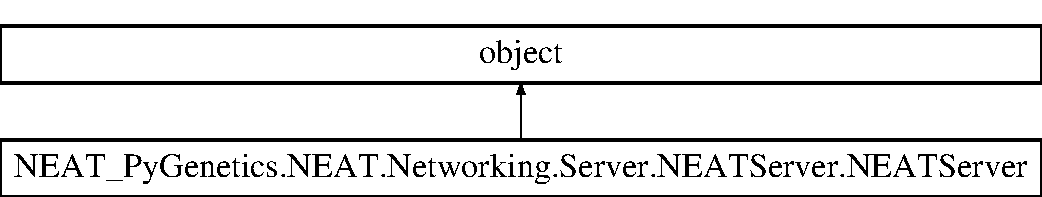
\includegraphics[height=2.000000cm]{classNEAT__PyGenetics_1_1NEAT_1_1Networking_1_1Server_1_1NEATServer_1_1NEATServer}
\end{center}
\end{figure}
\subsection*{Public Member Functions}
\begin{DoxyCompactItemize}
\item 
def \hyperlink{classNEAT__PyGenetics_1_1NEAT_1_1Networking_1_1Server_1_1NEATServer_1_1NEATServer_a45eb9c4003d9e0f4ae9c0e239423ddad}{\+\_\+\+\_\+init\+\_\+\+\_\+} (self)
\item 
def \hyperlink{classNEAT__PyGenetics_1_1NEAT_1_1Networking_1_1Server_1_1NEATServer_1_1NEATServer_a44ffcc6f56d71844827bd402bf4f0e63}{respond}
\item 
def \hyperlink{classNEAT__PyGenetics_1_1NEAT_1_1Networking_1_1Server_1_1NEATServer_1_1NEATServer_adf4c43680aa89998cf65bc6499f778a8}{fetch}
\end{DoxyCompactItemize}
\subsection*{Static Public Attributes}
\begin{DoxyCompactItemize}
\item 
\hyperlink{classNEAT__PyGenetics_1_1NEAT_1_1Networking_1_1Server_1_1NEATServer_1_1NEATServer_acbbd8416ba0d7139131ff0e553b20c3d}{time\+\_\+passed}
\item 
\hyperlink{classNEAT__PyGenetics_1_1NEAT_1_1Networking_1_1Server_1_1NEATServer_1_1NEATServer_abba58b32d9919608f5502e001dbd62dd}{starting\+\_\+time}
\end{DoxyCompactItemize}


\subsection{Constructor \& Destructor Documentation}
\index{N\+E\+A\+T\+\_\+\+Py\+Genetics\+::\+N\+E\+A\+T\+::\+Networking\+::\+Server\+::\+N\+E\+A\+T\+Server\+::\+N\+E\+A\+T\+Server@{N\+E\+A\+T\+\_\+\+Py\+Genetics\+::\+N\+E\+A\+T\+::\+Networking\+::\+Server\+::\+N\+E\+A\+T\+Server\+::\+N\+E\+A\+T\+Server}!\+\_\+\+\_\+init\+\_\+\+\_\+@{\+\_\+\+\_\+init\+\_\+\+\_\+}}
\index{\+\_\+\+\_\+init\+\_\+\+\_\+@{\+\_\+\+\_\+init\+\_\+\+\_\+}!N\+E\+A\+T\+\_\+\+Py\+Genetics\+::\+N\+E\+A\+T\+::\+Networking\+::\+Server\+::\+N\+E\+A\+T\+Server\+::\+N\+E\+A\+T\+Server@{N\+E\+A\+T\+\_\+\+Py\+Genetics\+::\+N\+E\+A\+T\+::\+Networking\+::\+Server\+::\+N\+E\+A\+T\+Server\+::\+N\+E\+A\+T\+Server}}
\subsubsection[{\texorpdfstring{\+\_\+\+\_\+init\+\_\+\+\_\+(self)}{__init__(self)}}]{\setlength{\rightskip}{0pt plus 5cm}def N\+E\+A\+T\+\_\+\+Py\+Genetics.\+N\+E\+A\+T.\+Networking.\+Server.\+N\+E\+A\+T\+Server.\+N\+E\+A\+T\+Server.\+\_\+\+\_\+init\+\_\+\+\_\+ (
\begin{DoxyParamCaption}
\item[{}]{self}
\end{DoxyParamCaption}
)}\hypertarget{classNEAT__PyGenetics_1_1NEAT_1_1Networking_1_1Server_1_1NEATServer_1_1NEATServer_a45eb9c4003d9e0f4ae9c0e239423ddad}{}\label{classNEAT__PyGenetics_1_1NEAT_1_1Networking_1_1Server_1_1NEATServer_1_1NEATServer_a45eb9c4003d9e0f4ae9c0e239423ddad}


\subsection{Member Function Documentation}
\index{N\+E\+A\+T\+\_\+\+Py\+Genetics\+::\+N\+E\+A\+T\+::\+Networking\+::\+Server\+::\+N\+E\+A\+T\+Server\+::\+N\+E\+A\+T\+Server@{N\+E\+A\+T\+\_\+\+Py\+Genetics\+::\+N\+E\+A\+T\+::\+Networking\+::\+Server\+::\+N\+E\+A\+T\+Server\+::\+N\+E\+A\+T\+Server}!fetch@{fetch}}
\index{fetch@{fetch}!N\+E\+A\+T\+\_\+\+Py\+Genetics\+::\+N\+E\+A\+T\+::\+Networking\+::\+Server\+::\+N\+E\+A\+T\+Server\+::\+N\+E\+A\+T\+Server@{N\+E\+A\+T\+\_\+\+Py\+Genetics\+::\+N\+E\+A\+T\+::\+Networking\+::\+Server\+::\+N\+E\+A\+T\+Server\+::\+N\+E\+A\+T\+Server}}
\subsubsection[{\texorpdfstring{fetch}{fetch}}]{\setlength{\rightskip}{0pt plus 5cm}def N\+E\+A\+T\+\_\+\+Py\+Genetics.\+N\+E\+A\+T.\+Networking.\+Server.\+N\+E\+A\+T\+Server.\+N\+E\+A\+T\+Server.\+fetch (
\begin{DoxyParamCaption}
\item[{}]{self, }
\item[{}]{timeout}
\end{DoxyParamCaption}
)}\hypertarget{classNEAT__PyGenetics_1_1NEAT_1_1Networking_1_1Server_1_1NEATServer_1_1NEATServer_adf4c43680aa89998cf65bc6499f778a8}{}\label{classNEAT__PyGenetics_1_1NEAT_1_1Networking_1_1Server_1_1NEATServer_1_1NEATServer_adf4c43680aa89998cf65bc6499f778a8}
\index{N\+E\+A\+T\+\_\+\+Py\+Genetics\+::\+N\+E\+A\+T\+::\+Networking\+::\+Server\+::\+N\+E\+A\+T\+Server\+::\+N\+E\+A\+T\+Server@{N\+E\+A\+T\+\_\+\+Py\+Genetics\+::\+N\+E\+A\+T\+::\+Networking\+::\+Server\+::\+N\+E\+A\+T\+Server\+::\+N\+E\+A\+T\+Server}!respond@{respond}}
\index{respond@{respond}!N\+E\+A\+T\+\_\+\+Py\+Genetics\+::\+N\+E\+A\+T\+::\+Networking\+::\+Server\+::\+N\+E\+A\+T\+Server\+::\+N\+E\+A\+T\+Server@{N\+E\+A\+T\+\_\+\+Py\+Genetics\+::\+N\+E\+A\+T\+::\+Networking\+::\+Server\+::\+N\+E\+A\+T\+Server\+::\+N\+E\+A\+T\+Server}}
\subsubsection[{\texorpdfstring{respond}{respond}}]{\setlength{\rightskip}{0pt plus 5cm}def N\+E\+A\+T\+\_\+\+Py\+Genetics.\+N\+E\+A\+T.\+Networking.\+Server.\+N\+E\+A\+T\+Server.\+N\+E\+A\+T\+Server.\+respond (
\begin{DoxyParamCaption}
\item[{}]{self, }
\item[{}]{command}
\end{DoxyParamCaption}
)}\hypertarget{classNEAT__PyGenetics_1_1NEAT_1_1Networking_1_1Server_1_1NEATServer_1_1NEATServer_a44ffcc6f56d71844827bd402bf4f0e63}{}\label{classNEAT__PyGenetics_1_1NEAT_1_1Networking_1_1Server_1_1NEATServer_1_1NEATServer_a44ffcc6f56d71844827bd402bf4f0e63}


\subsection{Member Data Documentation}
\index{N\+E\+A\+T\+\_\+\+Py\+Genetics\+::\+N\+E\+A\+T\+::\+Networking\+::\+Server\+::\+N\+E\+A\+T\+Server\+::\+N\+E\+A\+T\+Server@{N\+E\+A\+T\+\_\+\+Py\+Genetics\+::\+N\+E\+A\+T\+::\+Networking\+::\+Server\+::\+N\+E\+A\+T\+Server\+::\+N\+E\+A\+T\+Server}!starting\+\_\+time@{starting\+\_\+time}}
\index{starting\+\_\+time@{starting\+\_\+time}!N\+E\+A\+T\+\_\+\+Py\+Genetics\+::\+N\+E\+A\+T\+::\+Networking\+::\+Server\+::\+N\+E\+A\+T\+Server\+::\+N\+E\+A\+T\+Server@{N\+E\+A\+T\+\_\+\+Py\+Genetics\+::\+N\+E\+A\+T\+::\+Networking\+::\+Server\+::\+N\+E\+A\+T\+Server\+::\+N\+E\+A\+T\+Server}}
\subsubsection[{\texorpdfstring{starting\+\_\+time}{starting_time}}]{\setlength{\rightskip}{0pt plus 5cm}N\+E\+A\+T\+\_\+\+Py\+Genetics.\+N\+E\+A\+T.\+Networking.\+Server.\+N\+E\+A\+T\+Server.\+N\+E\+A\+T\+Server.\+starting\+\_\+time\hspace{0.3cm}{\ttfamily [static]}}\hypertarget{classNEAT__PyGenetics_1_1NEAT_1_1Networking_1_1Server_1_1NEATServer_1_1NEATServer_abba58b32d9919608f5502e001dbd62dd}{}\label{classNEAT__PyGenetics_1_1NEAT_1_1Networking_1_1Server_1_1NEATServer_1_1NEATServer_abba58b32d9919608f5502e001dbd62dd}
\index{N\+E\+A\+T\+\_\+\+Py\+Genetics\+::\+N\+E\+A\+T\+::\+Networking\+::\+Server\+::\+N\+E\+A\+T\+Server\+::\+N\+E\+A\+T\+Server@{N\+E\+A\+T\+\_\+\+Py\+Genetics\+::\+N\+E\+A\+T\+::\+Networking\+::\+Server\+::\+N\+E\+A\+T\+Server\+::\+N\+E\+A\+T\+Server}!time\+\_\+passed@{time\+\_\+passed}}
\index{time\+\_\+passed@{time\+\_\+passed}!N\+E\+A\+T\+\_\+\+Py\+Genetics\+::\+N\+E\+A\+T\+::\+Networking\+::\+Server\+::\+N\+E\+A\+T\+Server\+::\+N\+E\+A\+T\+Server@{N\+E\+A\+T\+\_\+\+Py\+Genetics\+::\+N\+E\+A\+T\+::\+Networking\+::\+Server\+::\+N\+E\+A\+T\+Server\+::\+N\+E\+A\+T\+Server}}
\subsubsection[{\texorpdfstring{time\+\_\+passed}{time_passed}}]{\setlength{\rightskip}{0pt plus 5cm}N\+E\+A\+T\+\_\+\+Py\+Genetics.\+N\+E\+A\+T.\+Networking.\+Server.\+N\+E\+A\+T\+Server.\+N\+E\+A\+T\+Server.\+time\+\_\+passed\hspace{0.3cm}{\ttfamily [static]}}\hypertarget{classNEAT__PyGenetics_1_1NEAT_1_1Networking_1_1Server_1_1NEATServer_1_1NEATServer_acbbd8416ba0d7139131ff0e553b20c3d}{}\label{classNEAT__PyGenetics_1_1NEAT_1_1Networking_1_1Server_1_1NEATServer_1_1NEATServer_acbbd8416ba0d7139131ff0e553b20c3d}


The documentation for this class was generated from the following file\+:\begin{DoxyCompactItemize}
\item 
N\+E\+A\+T/\+Networking/\+Server/\hyperlink{NEATServer_8py}{N\+E\+A\+T\+Server.\+py}\end{DoxyCompactItemize}

\hypertarget{classNEAT__PyGenetics_1_1NEAT_1_1ErrorHandling_1_1Exceptions_1_1NetworkProtocolException_1_1NetworkProtocolException}{}\section{N\+E\+A\+T\+\_\+\+Py\+Genetics.\+N\+E\+A\+T.\+Error\+Handling.\+Exceptions.\+Network\+Protocol\+Exception.\+Network\+Protocol\+Exception Class Reference}
\label{classNEAT__PyGenetics_1_1NEAT_1_1ErrorHandling_1_1Exceptions_1_1NetworkProtocolException_1_1NetworkProtocolException}\index{N\+E\+A\+T\+\_\+\+Py\+Genetics.\+N\+E\+A\+T.\+Error\+Handling.\+Exceptions.\+Network\+Protocol\+Exception.\+Network\+Protocol\+Exception@{N\+E\+A\+T\+\_\+\+Py\+Genetics.\+N\+E\+A\+T.\+Error\+Handling.\+Exceptions.\+Network\+Protocol\+Exception.\+Network\+Protocol\+Exception}}
Inheritance diagram for N\+E\+A\+T\+\_\+\+Py\+Genetics.\+N\+E\+A\+T.\+Error\+Handling.\+Exceptions.\+Network\+Protocol\+Exception.\+Network\+Protocol\+Exception\+:\begin{figure}[H]
\begin{center}
\leavevmode
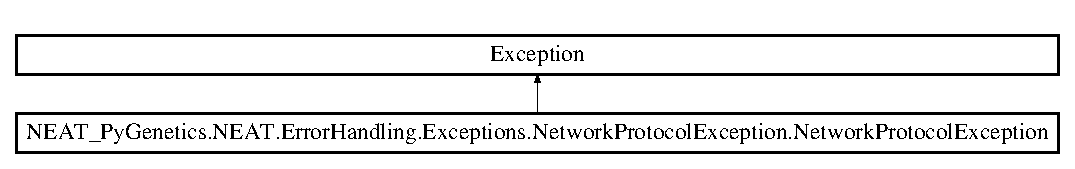
\includegraphics[height=1.824104cm]{classNEAT__PyGenetics_1_1NEAT_1_1ErrorHandling_1_1Exceptions_1_1NetworkProtocolException_1_1NetworkProtocolException}
\end{center}
\end{figure}
\subsection*{Public Member Functions}
\begin{DoxyCompactItemize}
\item 
def \hyperlink{classNEAT__PyGenetics_1_1NEAT_1_1ErrorHandling_1_1Exceptions_1_1NetworkProtocolException_1_1NetworkProtocolException_a9d12de9b98da65c1a683fe038e066e49}{\+\_\+\+\_\+init\+\_\+\+\_\+} (self, message, errors=None)
\end{DoxyCompactItemize}


\subsection{Constructor \& Destructor Documentation}
\index{N\+E\+A\+T\+\_\+\+Py\+Genetics\+::\+N\+E\+A\+T\+::\+Error\+Handling\+::\+Exceptions\+::\+Network\+Protocol\+Exception\+::\+Network\+Protocol\+Exception@{N\+E\+A\+T\+\_\+\+Py\+Genetics\+::\+N\+E\+A\+T\+::\+Error\+Handling\+::\+Exceptions\+::\+Network\+Protocol\+Exception\+::\+Network\+Protocol\+Exception}!\+\_\+\+\_\+init\+\_\+\+\_\+@{\+\_\+\+\_\+init\+\_\+\+\_\+}}
\index{\+\_\+\+\_\+init\+\_\+\+\_\+@{\+\_\+\+\_\+init\+\_\+\+\_\+}!N\+E\+A\+T\+\_\+\+Py\+Genetics\+::\+N\+E\+A\+T\+::\+Error\+Handling\+::\+Exceptions\+::\+Network\+Protocol\+Exception\+::\+Network\+Protocol\+Exception@{N\+E\+A\+T\+\_\+\+Py\+Genetics\+::\+N\+E\+A\+T\+::\+Error\+Handling\+::\+Exceptions\+::\+Network\+Protocol\+Exception\+::\+Network\+Protocol\+Exception}}
\subsubsection[{\texorpdfstring{\+\_\+\+\_\+init\+\_\+\+\_\+(self, message, errors=\+None)}{__init__(self, message, errors=None)}}]{\setlength{\rightskip}{0pt plus 5cm}def N\+E\+A\+T\+\_\+\+Py\+Genetics.\+N\+E\+A\+T.\+Error\+Handling.\+Exceptions.\+Network\+Protocol\+Exception.\+Network\+Protocol\+Exception.\+\_\+\+\_\+init\+\_\+\+\_\+ (
\begin{DoxyParamCaption}
\item[{}]{self, }
\item[{}]{message, }
\item[{}]{errors = {\ttfamily None}}
\end{DoxyParamCaption}
)}\hypertarget{classNEAT__PyGenetics_1_1NEAT_1_1ErrorHandling_1_1Exceptions_1_1NetworkProtocolException_1_1NetworkProtocolException_a9d12de9b98da65c1a683fe038e066e49}{}\label{classNEAT__PyGenetics_1_1NEAT_1_1ErrorHandling_1_1Exceptions_1_1NetworkProtocolException_1_1NetworkProtocolException_a9d12de9b98da65c1a683fe038e066e49}


The documentation for this class was generated from the following file\+:\begin{DoxyCompactItemize}
\item 
N\+E\+A\+T/\+Error\+Handling/\+Exceptions/\hyperlink{NetworkProtocolException_8py}{Network\+Protocol\+Exception.\+py}\end{DoxyCompactItemize}

\hypertarget{classNEAT__PyGenetics_1_1NEAT_1_1ErrorHandling_1_1Exceptions_1_1NetworkTimeoutException_1_1NetworkTimeoutException}{}\section{N\+E\+A\+T\+\_\+\+Py\+Genetics.\+N\+E\+A\+T.\+Error\+Handling.\+Exceptions.\+Network\+Timeout\+Exception.\+Network\+Timeout\+Exception Class Reference}
\label{classNEAT__PyGenetics_1_1NEAT_1_1ErrorHandling_1_1Exceptions_1_1NetworkTimeoutException_1_1NetworkTimeoutException}\index{N\+E\+A\+T\+\_\+\+Py\+Genetics.\+N\+E\+A\+T.\+Error\+Handling.\+Exceptions.\+Network\+Timeout\+Exception.\+Network\+Timeout\+Exception@{N\+E\+A\+T\+\_\+\+Py\+Genetics.\+N\+E\+A\+T.\+Error\+Handling.\+Exceptions.\+Network\+Timeout\+Exception.\+Network\+Timeout\+Exception}}
Inheritance diagram for N\+E\+A\+T\+\_\+\+Py\+Genetics.\+N\+E\+A\+T.\+Error\+Handling.\+Exceptions.\+Network\+Timeout\+Exception.\+Network\+Timeout\+Exception\+:\begin{figure}[H]
\begin{center}
\leavevmode
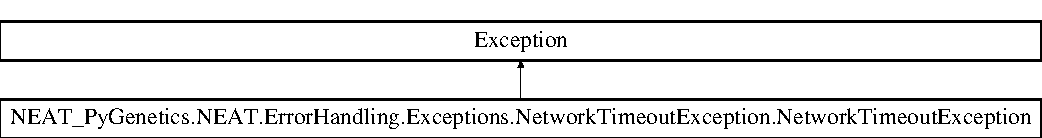
\includegraphics[height=1.848185cm]{classNEAT__PyGenetics_1_1NEAT_1_1ErrorHandling_1_1Exceptions_1_1NetworkTimeoutException_1_1NetworkTimeoutException}
\end{center}
\end{figure}
\subsection*{Public Member Functions}
\begin{DoxyCompactItemize}
\item 
def \hyperlink{classNEAT__PyGenetics_1_1NEAT_1_1ErrorHandling_1_1Exceptions_1_1NetworkTimeoutException_1_1NetworkTimeoutException_ac78b36042b085235de601a15a68ce98a}{\+\_\+\+\_\+init\+\_\+\+\_\+} (self, message=\char`\"{}\char`\"{}, errors=None)
\end{DoxyCompactItemize}


\subsection{Constructor \& Destructor Documentation}
\index{N\+E\+A\+T\+\_\+\+Py\+Genetics\+::\+N\+E\+A\+T\+::\+Error\+Handling\+::\+Exceptions\+::\+Network\+Timeout\+Exception\+::\+Network\+Timeout\+Exception@{N\+E\+A\+T\+\_\+\+Py\+Genetics\+::\+N\+E\+A\+T\+::\+Error\+Handling\+::\+Exceptions\+::\+Network\+Timeout\+Exception\+::\+Network\+Timeout\+Exception}!\+\_\+\+\_\+init\+\_\+\+\_\+@{\+\_\+\+\_\+init\+\_\+\+\_\+}}
\index{\+\_\+\+\_\+init\+\_\+\+\_\+@{\+\_\+\+\_\+init\+\_\+\+\_\+}!N\+E\+A\+T\+\_\+\+Py\+Genetics\+::\+N\+E\+A\+T\+::\+Error\+Handling\+::\+Exceptions\+::\+Network\+Timeout\+Exception\+::\+Network\+Timeout\+Exception@{N\+E\+A\+T\+\_\+\+Py\+Genetics\+::\+N\+E\+A\+T\+::\+Error\+Handling\+::\+Exceptions\+::\+Network\+Timeout\+Exception\+::\+Network\+Timeout\+Exception}}
\subsubsection[{\texorpdfstring{\+\_\+\+\_\+init\+\_\+\+\_\+(self, message="""", errors=\+None)}{__init__(self, message="", errors=None)}}]{\setlength{\rightskip}{0pt plus 5cm}def N\+E\+A\+T\+\_\+\+Py\+Genetics.\+N\+E\+A\+T.\+Error\+Handling.\+Exceptions.\+Network\+Timeout\+Exception.\+Network\+Timeout\+Exception.\+\_\+\+\_\+init\+\_\+\+\_\+ (
\begin{DoxyParamCaption}
\item[{}]{self, }
\item[{}]{message = {\ttfamily \char`\"{}\char`\"{}}, }
\item[{}]{errors = {\ttfamily None}}
\end{DoxyParamCaption}
)}\hypertarget{classNEAT__PyGenetics_1_1NEAT_1_1ErrorHandling_1_1Exceptions_1_1NetworkTimeoutException_1_1NetworkTimeoutException_ac78b36042b085235de601a15a68ce98a}{}\label{classNEAT__PyGenetics_1_1NEAT_1_1ErrorHandling_1_1Exceptions_1_1NetworkTimeoutException_1_1NetworkTimeoutException_ac78b36042b085235de601a15a68ce98a}


The documentation for this class was generated from the following file\+:\begin{DoxyCompactItemize}
\item 
N\+E\+A\+T/\+Error\+Handling/\+Exceptions/\hyperlink{NetworkTimeoutException_8py}{Network\+Timeout\+Exception.\+py}\end{DoxyCompactItemize}

\hypertarget{classNEAT__PyGenetics_1_1NEAT_1_1GenomeStructures_1_1SimulationStructure_1_1SimulationNodes_1_1Node}{}\section{N\+E\+A\+T\+\_\+\+Py\+Genetics.\+N\+E\+A\+T.\+Genome\+Structures.\+Simulation\+Structure.\+Simulation\+Nodes.\+Node Class Reference}
\label{classNEAT__PyGenetics_1_1NEAT_1_1GenomeStructures_1_1SimulationStructure_1_1SimulationNodes_1_1Node}\index{N\+E\+A\+T\+\_\+\+Py\+Genetics.\+N\+E\+A\+T.\+Genome\+Structures.\+Simulation\+Structure.\+Simulation\+Nodes.\+Node@{N\+E\+A\+T\+\_\+\+Py\+Genetics.\+N\+E\+A\+T.\+Genome\+Structures.\+Simulation\+Structure.\+Simulation\+Nodes.\+Node}}
Inheritance diagram for N\+E\+A\+T\+\_\+\+Py\+Genetics.\+N\+E\+A\+T.\+Genome\+Structures.\+Simulation\+Structure.\+Simulation\+Nodes.\+Node\+:\begin{figure}[H]
\begin{center}
\leavevmode
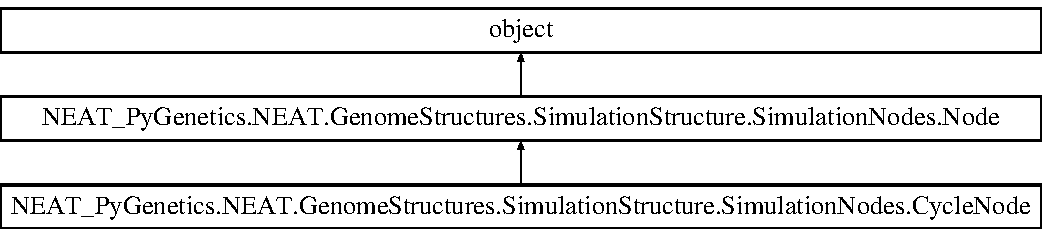
\includegraphics[height=3.000000cm]{classNEAT__PyGenetics_1_1NEAT_1_1GenomeStructures_1_1SimulationStructure_1_1SimulationNodes_1_1Node}
\end{center}
\end{figure}
\subsection*{Public Member Functions}
\begin{DoxyCompactItemize}
\item 
def \hyperlink{classNEAT__PyGenetics_1_1NEAT_1_1GenomeStructures_1_1SimulationStructure_1_1SimulationNodes_1_1Node_adc4a4683c2a06deaf2804d6f2745df3c}{\+\_\+\+\_\+init\+\_\+\+\_\+}
\item 
def \hyperlink{classNEAT__PyGenetics_1_1NEAT_1_1GenomeStructures_1_1SimulationStructure_1_1SimulationNodes_1_1Node_a97ac70897d562bce07c8395c17fe2a1b}{add\+\_\+successor}
\item 
def \hyperlink{classNEAT__PyGenetics_1_1NEAT_1_1GenomeStructures_1_1SimulationStructure_1_1SimulationNodes_1_1Node_a101dbc625ef502856902d623193e2901}{add\+\_\+successors}
\item 
def \hyperlink{classNEAT__PyGenetics_1_1NEAT_1_1GenomeStructures_1_1SimulationStructure_1_1SimulationNodes_1_1Node_ae2ad3e79c3b1a95bffd61b932f54f566}{reset} (self)
\item 
def \hyperlink{classNEAT__PyGenetics_1_1NEAT_1_1GenomeStructures_1_1SimulationStructure_1_1SimulationNodes_1_1Node_abc0a976efab6982a2630d01489554fde}{fire} (self)
\item 
def \hyperlink{classNEAT__PyGenetics_1_1NEAT_1_1GenomeStructures_1_1SimulationStructure_1_1SimulationNodes_1_1Node_aecc180ca33b3e3acd7601a3ad3e63b7d}{add\+\_\+value}
\end{DoxyCompactItemize}
\subsection*{Public Attributes}
\begin{DoxyCompactItemize}
\item 
\hyperlink{classNEAT__PyGenetics_1_1NEAT_1_1GenomeStructures_1_1SimulationStructure_1_1SimulationNodes_1_1Node_a7eb303cad09b69f01466fd6287c895c4}{successors}
\item 
\hyperlink{classNEAT__PyGenetics_1_1NEAT_1_1GenomeStructures_1_1SimulationStructure_1_1SimulationNodes_1_1Node_a0e8535438a367cd12a2eb47dee280f36}{weights}
\item 
\hyperlink{classNEAT__PyGenetics_1_1NEAT_1_1GenomeStructures_1_1SimulationStructure_1_1SimulationNodes_1_1Node_ae6a237c61d2c2118e6310f254c824490}{initial\+\_\+value}
\item 
\hyperlink{classNEAT__PyGenetics_1_1NEAT_1_1GenomeStructures_1_1SimulationStructure_1_1SimulationNodes_1_1Node_af25b687b957169788a4190545d6dd90c}{value}
\end{DoxyCompactItemize}


\subsection{Constructor \& Destructor Documentation}
\index{N\+E\+A\+T\+\_\+\+Py\+Genetics\+::\+N\+E\+A\+T\+::\+Genome\+Structures\+::\+Simulation\+Structure\+::\+Simulation\+Nodes\+::\+Node@{N\+E\+A\+T\+\_\+\+Py\+Genetics\+::\+N\+E\+A\+T\+::\+Genome\+Structures\+::\+Simulation\+Structure\+::\+Simulation\+Nodes\+::\+Node}!\+\_\+\+\_\+init\+\_\+\+\_\+@{\+\_\+\+\_\+init\+\_\+\+\_\+}}
\index{\+\_\+\+\_\+init\+\_\+\+\_\+@{\+\_\+\+\_\+init\+\_\+\+\_\+}!N\+E\+A\+T\+\_\+\+Py\+Genetics\+::\+N\+E\+A\+T\+::\+Genome\+Structures\+::\+Simulation\+Structure\+::\+Simulation\+Nodes\+::\+Node@{N\+E\+A\+T\+\_\+\+Py\+Genetics\+::\+N\+E\+A\+T\+::\+Genome\+Structures\+::\+Simulation\+Structure\+::\+Simulation\+Nodes\+::\+Node}}
\subsubsection[{\texorpdfstring{\+\_\+\+\_\+init\+\_\+\+\_\+}{__init__}}]{\setlength{\rightskip}{0pt plus 5cm}def N\+E\+A\+T\+\_\+\+Py\+Genetics.\+N\+E\+A\+T.\+Genome\+Structures.\+Simulation\+Structure.\+Simulation\+Nodes.\+Node.\+\_\+\+\_\+init\+\_\+\+\_\+ (
\begin{DoxyParamCaption}
\item[{}]{self, }
\item[{}]{initial\+\_\+value}
\end{DoxyParamCaption}
)}\hypertarget{classNEAT__PyGenetics_1_1NEAT_1_1GenomeStructures_1_1SimulationStructure_1_1SimulationNodes_1_1Node_adc4a4683c2a06deaf2804d6f2745df3c}{}\label{classNEAT__PyGenetics_1_1NEAT_1_1GenomeStructures_1_1SimulationStructure_1_1SimulationNodes_1_1Node_adc4a4683c2a06deaf2804d6f2745df3c}


\subsection{Member Function Documentation}
\index{N\+E\+A\+T\+\_\+\+Py\+Genetics\+::\+N\+E\+A\+T\+::\+Genome\+Structures\+::\+Simulation\+Structure\+::\+Simulation\+Nodes\+::\+Node@{N\+E\+A\+T\+\_\+\+Py\+Genetics\+::\+N\+E\+A\+T\+::\+Genome\+Structures\+::\+Simulation\+Structure\+::\+Simulation\+Nodes\+::\+Node}!add\+\_\+successor@{add\+\_\+successor}}
\index{add\+\_\+successor@{add\+\_\+successor}!N\+E\+A\+T\+\_\+\+Py\+Genetics\+::\+N\+E\+A\+T\+::\+Genome\+Structures\+::\+Simulation\+Structure\+::\+Simulation\+Nodes\+::\+Node@{N\+E\+A\+T\+\_\+\+Py\+Genetics\+::\+N\+E\+A\+T\+::\+Genome\+Structures\+::\+Simulation\+Structure\+::\+Simulation\+Nodes\+::\+Node}}
\subsubsection[{\texorpdfstring{add\+\_\+successor}{add_successor}}]{\setlength{\rightskip}{0pt plus 5cm}def N\+E\+A\+T\+\_\+\+Py\+Genetics.\+N\+E\+A\+T.\+Genome\+Structures.\+Simulation\+Structure.\+Simulation\+Nodes.\+Node.\+add\+\_\+successor (
\begin{DoxyParamCaption}
\item[{}]{self, }
\item[{}]{successor\+\_\+node}
\end{DoxyParamCaption}
)}\hypertarget{classNEAT__PyGenetics_1_1NEAT_1_1GenomeStructures_1_1SimulationStructure_1_1SimulationNodes_1_1Node_a97ac70897d562bce07c8395c17fe2a1b}{}\label{classNEAT__PyGenetics_1_1NEAT_1_1GenomeStructures_1_1SimulationStructure_1_1SimulationNodes_1_1Node_a97ac70897d562bce07c8395c17fe2a1b}
\index{N\+E\+A\+T\+\_\+\+Py\+Genetics\+::\+N\+E\+A\+T\+::\+Genome\+Structures\+::\+Simulation\+Structure\+::\+Simulation\+Nodes\+::\+Node@{N\+E\+A\+T\+\_\+\+Py\+Genetics\+::\+N\+E\+A\+T\+::\+Genome\+Structures\+::\+Simulation\+Structure\+::\+Simulation\+Nodes\+::\+Node}!add\+\_\+successors@{add\+\_\+successors}}
\index{add\+\_\+successors@{add\+\_\+successors}!N\+E\+A\+T\+\_\+\+Py\+Genetics\+::\+N\+E\+A\+T\+::\+Genome\+Structures\+::\+Simulation\+Structure\+::\+Simulation\+Nodes\+::\+Node@{N\+E\+A\+T\+\_\+\+Py\+Genetics\+::\+N\+E\+A\+T\+::\+Genome\+Structures\+::\+Simulation\+Structure\+::\+Simulation\+Nodes\+::\+Node}}
\subsubsection[{\texorpdfstring{add\+\_\+successors}{add_successors}}]{\setlength{\rightskip}{0pt plus 5cm}def N\+E\+A\+T\+\_\+\+Py\+Genetics.\+N\+E\+A\+T.\+Genome\+Structures.\+Simulation\+Structure.\+Simulation\+Nodes.\+Node.\+add\+\_\+successors (
\begin{DoxyParamCaption}
\item[{}]{self, }
\item[{}]{successor\+\_\+nodes}
\end{DoxyParamCaption}
)}\hypertarget{classNEAT__PyGenetics_1_1NEAT_1_1GenomeStructures_1_1SimulationStructure_1_1SimulationNodes_1_1Node_a101dbc625ef502856902d623193e2901}{}\label{classNEAT__PyGenetics_1_1NEAT_1_1GenomeStructures_1_1SimulationStructure_1_1SimulationNodes_1_1Node_a101dbc625ef502856902d623193e2901}
\index{N\+E\+A\+T\+\_\+\+Py\+Genetics\+::\+N\+E\+A\+T\+::\+Genome\+Structures\+::\+Simulation\+Structure\+::\+Simulation\+Nodes\+::\+Node@{N\+E\+A\+T\+\_\+\+Py\+Genetics\+::\+N\+E\+A\+T\+::\+Genome\+Structures\+::\+Simulation\+Structure\+::\+Simulation\+Nodes\+::\+Node}!add\+\_\+value@{add\+\_\+value}}
\index{add\+\_\+value@{add\+\_\+value}!N\+E\+A\+T\+\_\+\+Py\+Genetics\+::\+N\+E\+A\+T\+::\+Genome\+Structures\+::\+Simulation\+Structure\+::\+Simulation\+Nodes\+::\+Node@{N\+E\+A\+T\+\_\+\+Py\+Genetics\+::\+N\+E\+A\+T\+::\+Genome\+Structures\+::\+Simulation\+Structure\+::\+Simulation\+Nodes\+::\+Node}}
\subsubsection[{\texorpdfstring{add\+\_\+value}{add_value}}]{\setlength{\rightskip}{0pt plus 5cm}def N\+E\+A\+T\+\_\+\+Py\+Genetics.\+N\+E\+A\+T.\+Genome\+Structures.\+Simulation\+Structure.\+Simulation\+Nodes.\+Node.\+add\+\_\+value (
\begin{DoxyParamCaption}
\item[{}]{self, }
\item[{}]{value}
\end{DoxyParamCaption}
)}\hypertarget{classNEAT__PyGenetics_1_1NEAT_1_1GenomeStructures_1_1SimulationStructure_1_1SimulationNodes_1_1Node_aecc180ca33b3e3acd7601a3ad3e63b7d}{}\label{classNEAT__PyGenetics_1_1NEAT_1_1GenomeStructures_1_1SimulationStructure_1_1SimulationNodes_1_1Node_aecc180ca33b3e3acd7601a3ad3e63b7d}
\index{N\+E\+A\+T\+\_\+\+Py\+Genetics\+::\+N\+E\+A\+T\+::\+Genome\+Structures\+::\+Simulation\+Structure\+::\+Simulation\+Nodes\+::\+Node@{N\+E\+A\+T\+\_\+\+Py\+Genetics\+::\+N\+E\+A\+T\+::\+Genome\+Structures\+::\+Simulation\+Structure\+::\+Simulation\+Nodes\+::\+Node}!fire@{fire}}
\index{fire@{fire}!N\+E\+A\+T\+\_\+\+Py\+Genetics\+::\+N\+E\+A\+T\+::\+Genome\+Structures\+::\+Simulation\+Structure\+::\+Simulation\+Nodes\+::\+Node@{N\+E\+A\+T\+\_\+\+Py\+Genetics\+::\+N\+E\+A\+T\+::\+Genome\+Structures\+::\+Simulation\+Structure\+::\+Simulation\+Nodes\+::\+Node}}
\subsubsection[{\texorpdfstring{fire(self)}{fire(self)}}]{\setlength{\rightskip}{0pt plus 5cm}def N\+E\+A\+T\+\_\+\+Py\+Genetics.\+N\+E\+A\+T.\+Genome\+Structures.\+Simulation\+Structure.\+Simulation\+Nodes.\+Node.\+fire (
\begin{DoxyParamCaption}
\item[{}]{self, }
\item[{}]{None}
\end{DoxyParamCaption}
)}\hypertarget{classNEAT__PyGenetics_1_1NEAT_1_1GenomeStructures_1_1SimulationStructure_1_1SimulationNodes_1_1Node_abc0a976efab6982a2630d01489554fde}{}\label{classNEAT__PyGenetics_1_1NEAT_1_1GenomeStructures_1_1SimulationStructure_1_1SimulationNodes_1_1Node_abc0a976efab6982a2630d01489554fde}
\index{N\+E\+A\+T\+\_\+\+Py\+Genetics\+::\+N\+E\+A\+T\+::\+Genome\+Structures\+::\+Simulation\+Structure\+::\+Simulation\+Nodes\+::\+Node@{N\+E\+A\+T\+\_\+\+Py\+Genetics\+::\+N\+E\+A\+T\+::\+Genome\+Structures\+::\+Simulation\+Structure\+::\+Simulation\+Nodes\+::\+Node}!reset@{reset}}
\index{reset@{reset}!N\+E\+A\+T\+\_\+\+Py\+Genetics\+::\+N\+E\+A\+T\+::\+Genome\+Structures\+::\+Simulation\+Structure\+::\+Simulation\+Nodes\+::\+Node@{N\+E\+A\+T\+\_\+\+Py\+Genetics\+::\+N\+E\+A\+T\+::\+Genome\+Structures\+::\+Simulation\+Structure\+::\+Simulation\+Nodes\+::\+Node}}
\subsubsection[{\texorpdfstring{reset(self)}{reset(self)}}]{\setlength{\rightskip}{0pt plus 5cm}def N\+E\+A\+T\+\_\+\+Py\+Genetics.\+N\+E\+A\+T.\+Genome\+Structures.\+Simulation\+Structure.\+Simulation\+Nodes.\+Node.\+reset (
\begin{DoxyParamCaption}
\item[{}]{self, }
\item[{}]{None}
\end{DoxyParamCaption}
)}\hypertarget{classNEAT__PyGenetics_1_1NEAT_1_1GenomeStructures_1_1SimulationStructure_1_1SimulationNodes_1_1Node_ae2ad3e79c3b1a95bffd61b932f54f566}{}\label{classNEAT__PyGenetics_1_1NEAT_1_1GenomeStructures_1_1SimulationStructure_1_1SimulationNodes_1_1Node_ae2ad3e79c3b1a95bffd61b932f54f566}


\subsection{Member Data Documentation}
\index{N\+E\+A\+T\+\_\+\+Py\+Genetics\+::\+N\+E\+A\+T\+::\+Genome\+Structures\+::\+Simulation\+Structure\+::\+Simulation\+Nodes\+::\+Node@{N\+E\+A\+T\+\_\+\+Py\+Genetics\+::\+N\+E\+A\+T\+::\+Genome\+Structures\+::\+Simulation\+Structure\+::\+Simulation\+Nodes\+::\+Node}!initial\+\_\+value@{initial\+\_\+value}}
\index{initial\+\_\+value@{initial\+\_\+value}!N\+E\+A\+T\+\_\+\+Py\+Genetics\+::\+N\+E\+A\+T\+::\+Genome\+Structures\+::\+Simulation\+Structure\+::\+Simulation\+Nodes\+::\+Node@{N\+E\+A\+T\+\_\+\+Py\+Genetics\+::\+N\+E\+A\+T\+::\+Genome\+Structures\+::\+Simulation\+Structure\+::\+Simulation\+Nodes\+::\+Node}}
\subsubsection[{\texorpdfstring{initial\+\_\+value}{initial_value}}]{\setlength{\rightskip}{0pt plus 5cm}N\+E\+A\+T\+\_\+\+Py\+Genetics.\+N\+E\+A\+T.\+Genome\+Structures.\+Simulation\+Structure.\+Simulation\+Nodes.\+Node.\+initial\+\_\+value}\hypertarget{classNEAT__PyGenetics_1_1NEAT_1_1GenomeStructures_1_1SimulationStructure_1_1SimulationNodes_1_1Node_ae6a237c61d2c2118e6310f254c824490}{}\label{classNEAT__PyGenetics_1_1NEAT_1_1GenomeStructures_1_1SimulationStructure_1_1SimulationNodes_1_1Node_ae6a237c61d2c2118e6310f254c824490}
\index{N\+E\+A\+T\+\_\+\+Py\+Genetics\+::\+N\+E\+A\+T\+::\+Genome\+Structures\+::\+Simulation\+Structure\+::\+Simulation\+Nodes\+::\+Node@{N\+E\+A\+T\+\_\+\+Py\+Genetics\+::\+N\+E\+A\+T\+::\+Genome\+Structures\+::\+Simulation\+Structure\+::\+Simulation\+Nodes\+::\+Node}!successors@{successors}}
\index{successors@{successors}!N\+E\+A\+T\+\_\+\+Py\+Genetics\+::\+N\+E\+A\+T\+::\+Genome\+Structures\+::\+Simulation\+Structure\+::\+Simulation\+Nodes\+::\+Node@{N\+E\+A\+T\+\_\+\+Py\+Genetics\+::\+N\+E\+A\+T\+::\+Genome\+Structures\+::\+Simulation\+Structure\+::\+Simulation\+Nodes\+::\+Node}}
\subsubsection[{\texorpdfstring{successors}{successors}}]{\setlength{\rightskip}{0pt plus 5cm}N\+E\+A\+T\+\_\+\+Py\+Genetics.\+N\+E\+A\+T.\+Genome\+Structures.\+Simulation\+Structure.\+Simulation\+Nodes.\+Node.\+successors}\hypertarget{classNEAT__PyGenetics_1_1NEAT_1_1GenomeStructures_1_1SimulationStructure_1_1SimulationNodes_1_1Node_a7eb303cad09b69f01466fd6287c895c4}{}\label{classNEAT__PyGenetics_1_1NEAT_1_1GenomeStructures_1_1SimulationStructure_1_1SimulationNodes_1_1Node_a7eb303cad09b69f01466fd6287c895c4}
\index{N\+E\+A\+T\+\_\+\+Py\+Genetics\+::\+N\+E\+A\+T\+::\+Genome\+Structures\+::\+Simulation\+Structure\+::\+Simulation\+Nodes\+::\+Node@{N\+E\+A\+T\+\_\+\+Py\+Genetics\+::\+N\+E\+A\+T\+::\+Genome\+Structures\+::\+Simulation\+Structure\+::\+Simulation\+Nodes\+::\+Node}!value@{value}}
\index{value@{value}!N\+E\+A\+T\+\_\+\+Py\+Genetics\+::\+N\+E\+A\+T\+::\+Genome\+Structures\+::\+Simulation\+Structure\+::\+Simulation\+Nodes\+::\+Node@{N\+E\+A\+T\+\_\+\+Py\+Genetics\+::\+N\+E\+A\+T\+::\+Genome\+Structures\+::\+Simulation\+Structure\+::\+Simulation\+Nodes\+::\+Node}}
\subsubsection[{\texorpdfstring{value}{value}}]{\setlength{\rightskip}{0pt plus 5cm}N\+E\+A\+T\+\_\+\+Py\+Genetics.\+N\+E\+A\+T.\+Genome\+Structures.\+Simulation\+Structure.\+Simulation\+Nodes.\+Node.\+value}\hypertarget{classNEAT__PyGenetics_1_1NEAT_1_1GenomeStructures_1_1SimulationStructure_1_1SimulationNodes_1_1Node_af25b687b957169788a4190545d6dd90c}{}\label{classNEAT__PyGenetics_1_1NEAT_1_1GenomeStructures_1_1SimulationStructure_1_1SimulationNodes_1_1Node_af25b687b957169788a4190545d6dd90c}
\index{N\+E\+A\+T\+\_\+\+Py\+Genetics\+::\+N\+E\+A\+T\+::\+Genome\+Structures\+::\+Simulation\+Structure\+::\+Simulation\+Nodes\+::\+Node@{N\+E\+A\+T\+\_\+\+Py\+Genetics\+::\+N\+E\+A\+T\+::\+Genome\+Structures\+::\+Simulation\+Structure\+::\+Simulation\+Nodes\+::\+Node}!weights@{weights}}
\index{weights@{weights}!N\+E\+A\+T\+\_\+\+Py\+Genetics\+::\+N\+E\+A\+T\+::\+Genome\+Structures\+::\+Simulation\+Structure\+::\+Simulation\+Nodes\+::\+Node@{N\+E\+A\+T\+\_\+\+Py\+Genetics\+::\+N\+E\+A\+T\+::\+Genome\+Structures\+::\+Simulation\+Structure\+::\+Simulation\+Nodes\+::\+Node}}
\subsubsection[{\texorpdfstring{weights}{weights}}]{\setlength{\rightskip}{0pt plus 5cm}N\+E\+A\+T\+\_\+\+Py\+Genetics.\+N\+E\+A\+T.\+Genome\+Structures.\+Simulation\+Structure.\+Simulation\+Nodes.\+Node.\+weights}\hypertarget{classNEAT__PyGenetics_1_1NEAT_1_1GenomeStructures_1_1SimulationStructure_1_1SimulationNodes_1_1Node_a0e8535438a367cd12a2eb47dee280f36}{}\label{classNEAT__PyGenetics_1_1NEAT_1_1GenomeStructures_1_1SimulationStructure_1_1SimulationNodes_1_1Node_a0e8535438a367cd12a2eb47dee280f36}


The documentation for this class was generated from the following file\+:\begin{DoxyCompactItemize}
\item 
N\+E\+A\+T/\+Genome\+Structures/\+Simulation\+Structure/\hyperlink{SimulationNodes_8py}{Simulation\+Nodes.\+py}\end{DoxyCompactItemize}

\hypertarget{classNEAT__PyGenetics_1_1NEAT_1_1Networking_1_1Server_1_1NEATServer_1_1QueueWorker}{}\section{N\+E\+A\+T\+\_\+\+Py\+Genetics.\+N\+E\+A\+T.\+Networking.\+Server.\+N\+E\+A\+T\+Server.\+Queue\+Worker Class Reference}
\label{classNEAT__PyGenetics_1_1NEAT_1_1Networking_1_1Server_1_1NEATServer_1_1QueueWorker}\index{N\+E\+A\+T\+\_\+\+Py\+Genetics.\+N\+E\+A\+T.\+Networking.\+Server.\+N\+E\+A\+T\+Server.\+Queue\+Worker@{N\+E\+A\+T\+\_\+\+Py\+Genetics.\+N\+E\+A\+T.\+Networking.\+Server.\+N\+E\+A\+T\+Server.\+Queue\+Worker}}
Inheritance diagram for N\+E\+A\+T\+\_\+\+Py\+Genetics.\+N\+E\+A\+T.\+Networking.\+Server.\+N\+E\+A\+T\+Server.\+Queue\+Worker\+:\begin{figure}[H]
\begin{center}
\leavevmode
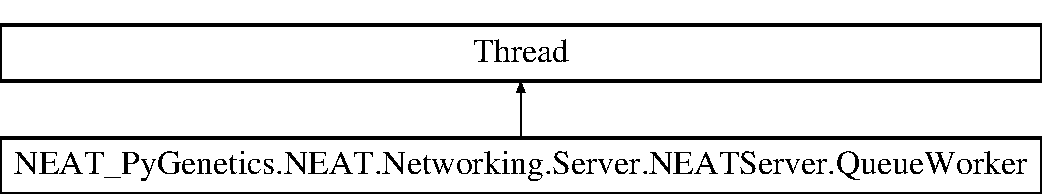
\includegraphics[height=2.000000cm]{classNEAT__PyGenetics_1_1NEAT_1_1Networking_1_1Server_1_1NEATServer_1_1QueueWorker}
\end{center}
\end{figure}
\subsection*{Public Member Functions}
\begin{DoxyCompactItemize}
\item 
def \hyperlink{classNEAT__PyGenetics_1_1NEAT_1_1Networking_1_1Server_1_1NEATServer_1_1QueueWorker_a413e2f230b433bfc4f137f1ae1a331e5}{\+\_\+\+\_\+init\+\_\+\+\_\+}
\item 
def \hyperlink{classNEAT__PyGenetics_1_1NEAT_1_1Networking_1_1Server_1_1NEATServer_1_1QueueWorker_a856d13880c0616f9b0c25b02788a54e3}{run} (self)
\end{DoxyCompactItemize}
\subsection*{Public Attributes}
\begin{DoxyCompactItemize}
\item 
\hyperlink{classNEAT__PyGenetics_1_1NEAT_1_1Networking_1_1Server_1_1NEATServer_1_1QueueWorker_ad5eb20f5b3bfb6a6aafa945bd5103c1b}{socket}
\end{DoxyCompactItemize}


\subsection{Constructor \& Destructor Documentation}
\index{N\+E\+A\+T\+\_\+\+Py\+Genetics\+::\+N\+E\+A\+T\+::\+Networking\+::\+Server\+::\+N\+E\+A\+T\+Server\+::\+Queue\+Worker@{N\+E\+A\+T\+\_\+\+Py\+Genetics\+::\+N\+E\+A\+T\+::\+Networking\+::\+Server\+::\+N\+E\+A\+T\+Server\+::\+Queue\+Worker}!\+\_\+\+\_\+init\+\_\+\+\_\+@{\+\_\+\+\_\+init\+\_\+\+\_\+}}
\index{\+\_\+\+\_\+init\+\_\+\+\_\+@{\+\_\+\+\_\+init\+\_\+\+\_\+}!N\+E\+A\+T\+\_\+\+Py\+Genetics\+::\+N\+E\+A\+T\+::\+Networking\+::\+Server\+::\+N\+E\+A\+T\+Server\+::\+Queue\+Worker@{N\+E\+A\+T\+\_\+\+Py\+Genetics\+::\+N\+E\+A\+T\+::\+Networking\+::\+Server\+::\+N\+E\+A\+T\+Server\+::\+Queue\+Worker}}
\subsubsection[{\texorpdfstring{\+\_\+\+\_\+init\+\_\+\+\_\+}{__init__}}]{\setlength{\rightskip}{0pt plus 5cm}def N\+E\+A\+T\+\_\+\+Py\+Genetics.\+N\+E\+A\+T.\+Networking.\+Server.\+N\+E\+A\+T\+Server.\+Queue\+Worker.\+\_\+\+\_\+init\+\_\+\+\_\+ (
\begin{DoxyParamCaption}
\item[{}]{self, }
\item[{}]{queue}
\end{DoxyParamCaption}
)}\hypertarget{classNEAT__PyGenetics_1_1NEAT_1_1Networking_1_1Server_1_1NEATServer_1_1QueueWorker_a413e2f230b433bfc4f137f1ae1a331e5}{}\label{classNEAT__PyGenetics_1_1NEAT_1_1Networking_1_1Server_1_1NEATServer_1_1QueueWorker_a413e2f230b433bfc4f137f1ae1a331e5}


\subsection{Member Function Documentation}
\index{N\+E\+A\+T\+\_\+\+Py\+Genetics\+::\+N\+E\+A\+T\+::\+Networking\+::\+Server\+::\+N\+E\+A\+T\+Server\+::\+Queue\+Worker@{N\+E\+A\+T\+\_\+\+Py\+Genetics\+::\+N\+E\+A\+T\+::\+Networking\+::\+Server\+::\+N\+E\+A\+T\+Server\+::\+Queue\+Worker}!run@{run}}
\index{run@{run}!N\+E\+A\+T\+\_\+\+Py\+Genetics\+::\+N\+E\+A\+T\+::\+Networking\+::\+Server\+::\+N\+E\+A\+T\+Server\+::\+Queue\+Worker@{N\+E\+A\+T\+\_\+\+Py\+Genetics\+::\+N\+E\+A\+T\+::\+Networking\+::\+Server\+::\+N\+E\+A\+T\+Server\+::\+Queue\+Worker}}
\subsubsection[{\texorpdfstring{run(self)}{run(self)}}]{\setlength{\rightskip}{0pt plus 5cm}def N\+E\+A\+T\+\_\+\+Py\+Genetics.\+N\+E\+A\+T.\+Networking.\+Server.\+N\+E\+A\+T\+Server.\+Queue\+Worker.\+run (
\begin{DoxyParamCaption}
\item[{}]{self}
\end{DoxyParamCaption}
)}\hypertarget{classNEAT__PyGenetics_1_1NEAT_1_1Networking_1_1Server_1_1NEATServer_1_1QueueWorker_a856d13880c0616f9b0c25b02788a54e3}{}\label{classNEAT__PyGenetics_1_1NEAT_1_1Networking_1_1Server_1_1NEATServer_1_1QueueWorker_a856d13880c0616f9b0c25b02788a54e3}


\subsection{Member Data Documentation}
\index{N\+E\+A\+T\+\_\+\+Py\+Genetics\+::\+N\+E\+A\+T\+::\+Networking\+::\+Server\+::\+N\+E\+A\+T\+Server\+::\+Queue\+Worker@{N\+E\+A\+T\+\_\+\+Py\+Genetics\+::\+N\+E\+A\+T\+::\+Networking\+::\+Server\+::\+N\+E\+A\+T\+Server\+::\+Queue\+Worker}!socket@{socket}}
\index{socket@{socket}!N\+E\+A\+T\+\_\+\+Py\+Genetics\+::\+N\+E\+A\+T\+::\+Networking\+::\+Server\+::\+N\+E\+A\+T\+Server\+::\+Queue\+Worker@{N\+E\+A\+T\+\_\+\+Py\+Genetics\+::\+N\+E\+A\+T\+::\+Networking\+::\+Server\+::\+N\+E\+A\+T\+Server\+::\+Queue\+Worker}}
\subsubsection[{\texorpdfstring{socket}{socket}}]{\setlength{\rightskip}{0pt plus 5cm}N\+E\+A\+T\+\_\+\+Py\+Genetics.\+N\+E\+A\+T.\+Networking.\+Server.\+N\+E\+A\+T\+Server.\+Queue\+Worker.\+socket}\hypertarget{classNEAT__PyGenetics_1_1NEAT_1_1Networking_1_1Server_1_1NEATServer_1_1QueueWorker_ad5eb20f5b3bfb6a6aafa945bd5103c1b}{}\label{classNEAT__PyGenetics_1_1NEAT_1_1Networking_1_1Server_1_1NEATServer_1_1QueueWorker_ad5eb20f5b3bfb6a6aafa945bd5103c1b}


The documentation for this class was generated from the following file\+:\begin{DoxyCompactItemize}
\item 
N\+E\+A\+T/\+Networking/\+Server/\hyperlink{NEATServer_8py}{N\+E\+A\+T\+Server.\+py}\end{DoxyCompactItemize}

\hypertarget{classNEAT__PyGenetics_1_1NEAT_1_1ErrorHandling_1_1Exceptions_1_1SerializationException_1_1SerializationException}{}\section{N\+E\+A\+T\+\_\+\+Py\+Genetics.\+N\+E\+A\+T.\+Error\+Handling.\+Exceptions.\+Serialization\+Exception.\+Serialization\+Exception Class Reference}
\label{classNEAT__PyGenetics_1_1NEAT_1_1ErrorHandling_1_1Exceptions_1_1SerializationException_1_1SerializationException}\index{N\+E\+A\+T\+\_\+\+Py\+Genetics.\+N\+E\+A\+T.\+Error\+Handling.\+Exceptions.\+Serialization\+Exception.\+Serialization\+Exception@{N\+E\+A\+T\+\_\+\+Py\+Genetics.\+N\+E\+A\+T.\+Error\+Handling.\+Exceptions.\+Serialization\+Exception.\+Serialization\+Exception}}
Inheritance diagram for N\+E\+A\+T\+\_\+\+Py\+Genetics.\+N\+E\+A\+T.\+Error\+Handling.\+Exceptions.\+Serialization\+Exception.\+Serialization\+Exception\+:\begin{figure}[H]
\begin{center}
\leavevmode
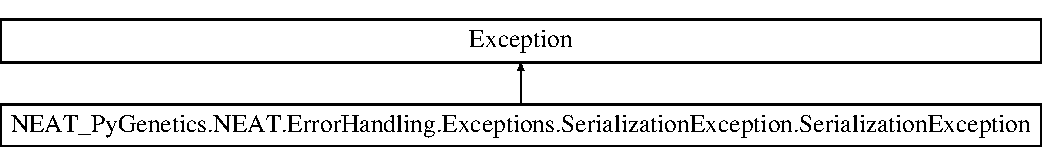
\includegraphics[height=1.978799cm]{classNEAT__PyGenetics_1_1NEAT_1_1ErrorHandling_1_1Exceptions_1_1SerializationException_1_1SerializationException}
\end{center}
\end{figure}
\subsection*{Public Member Functions}
\begin{DoxyCompactItemize}
\item 
def \hyperlink{classNEAT__PyGenetics_1_1NEAT_1_1ErrorHandling_1_1Exceptions_1_1SerializationException_1_1SerializationException_ada817ecebb49fc5dc085531462eef9a0}{\+\_\+\+\_\+init\+\_\+\+\_\+} (self, message=\char`\"{}\char`\"{}, errors=None)
\end{DoxyCompactItemize}


\subsection{Constructor \& Destructor Documentation}
\index{N\+E\+A\+T\+\_\+\+Py\+Genetics\+::\+N\+E\+A\+T\+::\+Error\+Handling\+::\+Exceptions\+::\+Serialization\+Exception\+::\+Serialization\+Exception@{N\+E\+A\+T\+\_\+\+Py\+Genetics\+::\+N\+E\+A\+T\+::\+Error\+Handling\+::\+Exceptions\+::\+Serialization\+Exception\+::\+Serialization\+Exception}!\+\_\+\+\_\+init\+\_\+\+\_\+@{\+\_\+\+\_\+init\+\_\+\+\_\+}}
\index{\+\_\+\+\_\+init\+\_\+\+\_\+@{\+\_\+\+\_\+init\+\_\+\+\_\+}!N\+E\+A\+T\+\_\+\+Py\+Genetics\+::\+N\+E\+A\+T\+::\+Error\+Handling\+::\+Exceptions\+::\+Serialization\+Exception\+::\+Serialization\+Exception@{N\+E\+A\+T\+\_\+\+Py\+Genetics\+::\+N\+E\+A\+T\+::\+Error\+Handling\+::\+Exceptions\+::\+Serialization\+Exception\+::\+Serialization\+Exception}}
\subsubsection[{\texorpdfstring{\+\_\+\+\_\+init\+\_\+\+\_\+(self, message="""", errors=\+None)}{__init__(self, message="", errors=None)}}]{\setlength{\rightskip}{0pt plus 5cm}def N\+E\+A\+T\+\_\+\+Py\+Genetics.\+N\+E\+A\+T.\+Error\+Handling.\+Exceptions.\+Serialization\+Exception.\+Serialization\+Exception.\+\_\+\+\_\+init\+\_\+\+\_\+ (
\begin{DoxyParamCaption}
\item[{}]{self, }
\item[{}]{message = {\ttfamily \char`\"{}\char`\"{}}, }
\item[{}]{errors = {\ttfamily None}}
\end{DoxyParamCaption}
)}\hypertarget{classNEAT__PyGenetics_1_1NEAT_1_1ErrorHandling_1_1Exceptions_1_1SerializationException_1_1SerializationException_ada817ecebb49fc5dc085531462eef9a0}{}\label{classNEAT__PyGenetics_1_1NEAT_1_1ErrorHandling_1_1Exceptions_1_1SerializationException_1_1SerializationException_ada817ecebb49fc5dc085531462eef9a0}


The documentation for this class was generated from the following file\+:\begin{DoxyCompactItemize}
\item 
N\+E\+A\+T/\+Error\+Handling/\+Exceptions/\hyperlink{SerializationException_8py}{Serialization\+Exception.\+py}\end{DoxyCompactItemize}

\hypertarget{classNEAT__PyGenetics_1_1NEAT_1_1Networking_1_1Commands_1_1SetFitnessValuesCommand_1_1SetFitnessValuesCommand}{}\section{N\+E\+A\+T\+\_\+\+Py\+Genetics.\+N\+E\+A\+T.\+Networking.\+Commands.\+Set\+Fitness\+Values\+Command.\+Set\+Fitness\+Values\+Command Class Reference}
\label{classNEAT__PyGenetics_1_1NEAT_1_1Networking_1_1Commands_1_1SetFitnessValuesCommand_1_1SetFitnessValuesCommand}\index{N\+E\+A\+T\+\_\+\+Py\+Genetics.\+N\+E\+A\+T.\+Networking.\+Commands.\+Set\+Fitness\+Values\+Command.\+Set\+Fitness\+Values\+Command@{N\+E\+A\+T\+\_\+\+Py\+Genetics.\+N\+E\+A\+T.\+Networking.\+Commands.\+Set\+Fitness\+Values\+Command.\+Set\+Fitness\+Values\+Command}}
Inheritance diagram for N\+E\+A\+T\+\_\+\+Py\+Genetics.\+N\+E\+A\+T.\+Networking.\+Commands.\+Set\+Fitness\+Values\+Command.\+Set\+Fitness\+Values\+Command\+:\begin{figure}[H]
\begin{center}
\leavevmode
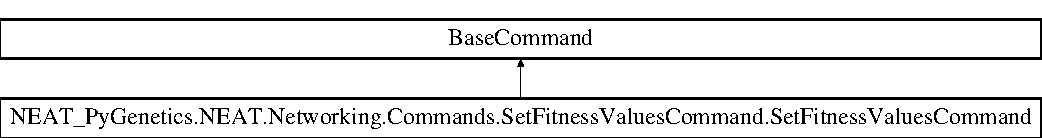
\includegraphics[height=1.851240cm]{classNEAT__PyGenetics_1_1NEAT_1_1Networking_1_1Commands_1_1SetFitnessValuesCommand_1_1SetFitnessValuesCommand}
\end{center}
\end{figure}
\subsection*{Public Member Functions}
\begin{DoxyCompactItemize}
\item 
def \hyperlink{classNEAT__PyGenetics_1_1NEAT_1_1Networking_1_1Commands_1_1SetFitnessValuesCommand_1_1SetFitnessValuesCommand_af1878c6d7a7fcb3d42693ebf5ab9a8f9}{\+\_\+\+\_\+init\+\_\+\+\_\+} (self)
\item 
def \hyperlink{classNEAT__PyGenetics_1_1NEAT_1_1Networking_1_1Commands_1_1SetFitnessValuesCommand_1_1SetFitnessValuesCommand_ad422d62ec35756ac1375c71222e902ba}{set\+\_\+fitness\+\_\+values}
\item 
def \hyperlink{classNEAT__PyGenetics_1_1NEAT_1_1Networking_1_1Commands_1_1SetFitnessValuesCommand_1_1SetFitnessValuesCommand_a44c78bd4ea207b596aa62cf5e6ee5ebc}{set\+\_\+fitness\+\_\+value}
\end{DoxyCompactItemize}


\subsection{Constructor \& Destructor Documentation}
\index{N\+E\+A\+T\+\_\+\+Py\+Genetics\+::\+N\+E\+A\+T\+::\+Networking\+::\+Commands\+::\+Set\+Fitness\+Values\+Command\+::\+Set\+Fitness\+Values\+Command@{N\+E\+A\+T\+\_\+\+Py\+Genetics\+::\+N\+E\+A\+T\+::\+Networking\+::\+Commands\+::\+Set\+Fitness\+Values\+Command\+::\+Set\+Fitness\+Values\+Command}!\+\_\+\+\_\+init\+\_\+\+\_\+@{\+\_\+\+\_\+init\+\_\+\+\_\+}}
\index{\+\_\+\+\_\+init\+\_\+\+\_\+@{\+\_\+\+\_\+init\+\_\+\+\_\+}!N\+E\+A\+T\+\_\+\+Py\+Genetics\+::\+N\+E\+A\+T\+::\+Networking\+::\+Commands\+::\+Set\+Fitness\+Values\+Command\+::\+Set\+Fitness\+Values\+Command@{N\+E\+A\+T\+\_\+\+Py\+Genetics\+::\+N\+E\+A\+T\+::\+Networking\+::\+Commands\+::\+Set\+Fitness\+Values\+Command\+::\+Set\+Fitness\+Values\+Command}}
\subsubsection[{\texorpdfstring{\+\_\+\+\_\+init\+\_\+\+\_\+(self)}{__init__(self)}}]{\setlength{\rightskip}{0pt plus 5cm}def N\+E\+A\+T\+\_\+\+Py\+Genetics.\+N\+E\+A\+T.\+Networking.\+Commands.\+Set\+Fitness\+Values\+Command.\+Set\+Fitness\+Values\+Command.\+\_\+\+\_\+init\+\_\+\+\_\+ (
\begin{DoxyParamCaption}
\item[{}]{self}
\end{DoxyParamCaption}
)}\hypertarget{classNEAT__PyGenetics_1_1NEAT_1_1Networking_1_1Commands_1_1SetFitnessValuesCommand_1_1SetFitnessValuesCommand_af1878c6d7a7fcb3d42693ebf5ab9a8f9}{}\label{classNEAT__PyGenetics_1_1NEAT_1_1Networking_1_1Commands_1_1SetFitnessValuesCommand_1_1SetFitnessValuesCommand_af1878c6d7a7fcb3d42693ebf5ab9a8f9}


\subsection{Member Function Documentation}
\index{N\+E\+A\+T\+\_\+\+Py\+Genetics\+::\+N\+E\+A\+T\+::\+Networking\+::\+Commands\+::\+Set\+Fitness\+Values\+Command\+::\+Set\+Fitness\+Values\+Command@{N\+E\+A\+T\+\_\+\+Py\+Genetics\+::\+N\+E\+A\+T\+::\+Networking\+::\+Commands\+::\+Set\+Fitness\+Values\+Command\+::\+Set\+Fitness\+Values\+Command}!set\+\_\+fitness\+\_\+value@{set\+\_\+fitness\+\_\+value}}
\index{set\+\_\+fitness\+\_\+value@{set\+\_\+fitness\+\_\+value}!N\+E\+A\+T\+\_\+\+Py\+Genetics\+::\+N\+E\+A\+T\+::\+Networking\+::\+Commands\+::\+Set\+Fitness\+Values\+Command\+::\+Set\+Fitness\+Values\+Command@{N\+E\+A\+T\+\_\+\+Py\+Genetics\+::\+N\+E\+A\+T\+::\+Networking\+::\+Commands\+::\+Set\+Fitness\+Values\+Command\+::\+Set\+Fitness\+Values\+Command}}
\subsubsection[{\texorpdfstring{set\+\_\+fitness\+\_\+value}{set_fitness_value}}]{\setlength{\rightskip}{0pt plus 5cm}def N\+E\+A\+T\+\_\+\+Py\+Genetics.\+N\+E\+A\+T.\+Networking.\+Commands.\+Set\+Fitness\+Values\+Command.\+Set\+Fitness\+Values\+Command.\+set\+\_\+fitness\+\_\+value (
\begin{DoxyParamCaption}
\item[{}]{self, }
\item[{}]{genome\+\_\+id}
\end{DoxyParamCaption}
)}\hypertarget{classNEAT__PyGenetics_1_1NEAT_1_1Networking_1_1Commands_1_1SetFitnessValuesCommand_1_1SetFitnessValuesCommand_a44c78bd4ea207b596aa62cf5e6ee5ebc}{}\label{classNEAT__PyGenetics_1_1NEAT_1_1Networking_1_1Commands_1_1SetFitnessValuesCommand_1_1SetFitnessValuesCommand_a44c78bd4ea207b596aa62cf5e6ee5ebc}
\index{N\+E\+A\+T\+\_\+\+Py\+Genetics\+::\+N\+E\+A\+T\+::\+Networking\+::\+Commands\+::\+Set\+Fitness\+Values\+Command\+::\+Set\+Fitness\+Values\+Command@{N\+E\+A\+T\+\_\+\+Py\+Genetics\+::\+N\+E\+A\+T\+::\+Networking\+::\+Commands\+::\+Set\+Fitness\+Values\+Command\+::\+Set\+Fitness\+Values\+Command}!set\+\_\+fitness\+\_\+values@{set\+\_\+fitness\+\_\+values}}
\index{set\+\_\+fitness\+\_\+values@{set\+\_\+fitness\+\_\+values}!N\+E\+A\+T\+\_\+\+Py\+Genetics\+::\+N\+E\+A\+T\+::\+Networking\+::\+Commands\+::\+Set\+Fitness\+Values\+Command\+::\+Set\+Fitness\+Values\+Command@{N\+E\+A\+T\+\_\+\+Py\+Genetics\+::\+N\+E\+A\+T\+::\+Networking\+::\+Commands\+::\+Set\+Fitness\+Values\+Command\+::\+Set\+Fitness\+Values\+Command}}
\subsubsection[{\texorpdfstring{set\+\_\+fitness\+\_\+values}{set_fitness_values}}]{\setlength{\rightskip}{0pt plus 5cm}def N\+E\+A\+T\+\_\+\+Py\+Genetics.\+N\+E\+A\+T.\+Networking.\+Commands.\+Set\+Fitness\+Values\+Command.\+Set\+Fitness\+Values\+Command.\+set\+\_\+fitness\+\_\+values (
\begin{DoxyParamCaption}
\item[{}]{self, }
\item[{}]{fitness\+\_\+values}
\end{DoxyParamCaption}
)}\hypertarget{classNEAT__PyGenetics_1_1NEAT_1_1Networking_1_1Commands_1_1SetFitnessValuesCommand_1_1SetFitnessValuesCommand_ad422d62ec35756ac1375c71222e902ba}{}\label{classNEAT__PyGenetics_1_1NEAT_1_1Networking_1_1Commands_1_1SetFitnessValuesCommand_1_1SetFitnessValuesCommand_ad422d62ec35756ac1375c71222e902ba}


The documentation for this class was generated from the following file\+:\begin{DoxyCompactItemize}
\item 
N\+E\+A\+T/\+Networking/\+Commands/\hyperlink{SetFitnessValuesCommand_8py}{Set\+Fitness\+Values\+Command.\+py}\end{DoxyCompactItemize}

\hypertarget{classNEAT__PyGenetics_1_1NEAT_1_1Networking_1_1Commands_1_1SetInputsCommand_1_1SetInputsCommand}{}\section{N\+E\+A\+T\+\_\+\+Py\+Genetics.\+N\+E\+A\+T.\+Networking.\+Commands.\+Set\+Inputs\+Command.\+Set\+Inputs\+Command Class Reference}
\label{classNEAT__PyGenetics_1_1NEAT_1_1Networking_1_1Commands_1_1SetInputsCommand_1_1SetInputsCommand}\index{N\+E\+A\+T\+\_\+\+Py\+Genetics.\+N\+E\+A\+T.\+Networking.\+Commands.\+Set\+Inputs\+Command.\+Set\+Inputs\+Command@{N\+E\+A\+T\+\_\+\+Py\+Genetics.\+N\+E\+A\+T.\+Networking.\+Commands.\+Set\+Inputs\+Command.\+Set\+Inputs\+Command}}
Inheritance diagram for N\+E\+A\+T\+\_\+\+Py\+Genetics.\+N\+E\+A\+T.\+Networking.\+Commands.\+Set\+Inputs\+Command.\+Set\+Inputs\+Command\+:\begin{figure}[H]
\begin{center}
\leavevmode
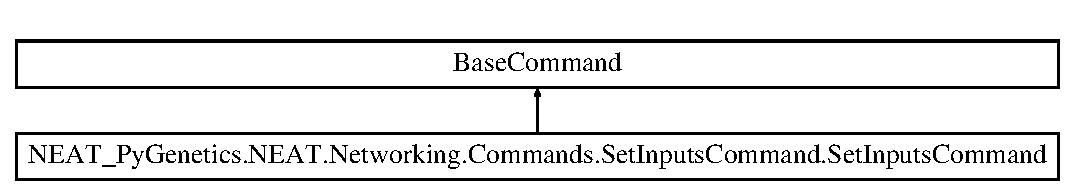
\includegraphics[height=2.000000cm]{classNEAT__PyGenetics_1_1NEAT_1_1Networking_1_1Commands_1_1SetInputsCommand_1_1SetInputsCommand}
\end{center}
\end{figure}
\subsection*{Public Member Functions}
\begin{DoxyCompactItemize}
\item 
def \hyperlink{classNEAT__PyGenetics_1_1NEAT_1_1Networking_1_1Commands_1_1SetInputsCommand_1_1SetInputsCommand_a8976dadea27ff8c738c32b2a8c42acde}{\+\_\+\+\_\+init\+\_\+\+\_\+} (self)
\item 
def \hyperlink{classNEAT__PyGenetics_1_1NEAT_1_1Networking_1_1Commands_1_1SetInputsCommand_1_1SetInputsCommand_a610420d005c225778fa1be622cd3843a}{set\+\_\+inputs}
\end{DoxyCompactItemize}


\subsection{Constructor \& Destructor Documentation}
\index{N\+E\+A\+T\+\_\+\+Py\+Genetics\+::\+N\+E\+A\+T\+::\+Networking\+::\+Commands\+::\+Set\+Inputs\+Command\+::\+Set\+Inputs\+Command@{N\+E\+A\+T\+\_\+\+Py\+Genetics\+::\+N\+E\+A\+T\+::\+Networking\+::\+Commands\+::\+Set\+Inputs\+Command\+::\+Set\+Inputs\+Command}!\+\_\+\+\_\+init\+\_\+\+\_\+@{\+\_\+\+\_\+init\+\_\+\+\_\+}}
\index{\+\_\+\+\_\+init\+\_\+\+\_\+@{\+\_\+\+\_\+init\+\_\+\+\_\+}!N\+E\+A\+T\+\_\+\+Py\+Genetics\+::\+N\+E\+A\+T\+::\+Networking\+::\+Commands\+::\+Set\+Inputs\+Command\+::\+Set\+Inputs\+Command@{N\+E\+A\+T\+\_\+\+Py\+Genetics\+::\+N\+E\+A\+T\+::\+Networking\+::\+Commands\+::\+Set\+Inputs\+Command\+::\+Set\+Inputs\+Command}}
\subsubsection[{\texorpdfstring{\+\_\+\+\_\+init\+\_\+\+\_\+(self)}{__init__(self)}}]{\setlength{\rightskip}{0pt plus 5cm}def N\+E\+A\+T\+\_\+\+Py\+Genetics.\+N\+E\+A\+T.\+Networking.\+Commands.\+Set\+Inputs\+Command.\+Set\+Inputs\+Command.\+\_\+\+\_\+init\+\_\+\+\_\+ (
\begin{DoxyParamCaption}
\item[{}]{self}
\end{DoxyParamCaption}
)}\hypertarget{classNEAT__PyGenetics_1_1NEAT_1_1Networking_1_1Commands_1_1SetInputsCommand_1_1SetInputsCommand_a8976dadea27ff8c738c32b2a8c42acde}{}\label{classNEAT__PyGenetics_1_1NEAT_1_1Networking_1_1Commands_1_1SetInputsCommand_1_1SetInputsCommand_a8976dadea27ff8c738c32b2a8c42acde}


\subsection{Member Function Documentation}
\index{N\+E\+A\+T\+\_\+\+Py\+Genetics\+::\+N\+E\+A\+T\+::\+Networking\+::\+Commands\+::\+Set\+Inputs\+Command\+::\+Set\+Inputs\+Command@{N\+E\+A\+T\+\_\+\+Py\+Genetics\+::\+N\+E\+A\+T\+::\+Networking\+::\+Commands\+::\+Set\+Inputs\+Command\+::\+Set\+Inputs\+Command}!set\+\_\+inputs@{set\+\_\+inputs}}
\index{set\+\_\+inputs@{set\+\_\+inputs}!N\+E\+A\+T\+\_\+\+Py\+Genetics\+::\+N\+E\+A\+T\+::\+Networking\+::\+Commands\+::\+Set\+Inputs\+Command\+::\+Set\+Inputs\+Command@{N\+E\+A\+T\+\_\+\+Py\+Genetics\+::\+N\+E\+A\+T\+::\+Networking\+::\+Commands\+::\+Set\+Inputs\+Command\+::\+Set\+Inputs\+Command}}
\subsubsection[{\texorpdfstring{set\+\_\+inputs}{set_inputs}}]{\setlength{\rightskip}{0pt plus 5cm}def N\+E\+A\+T\+\_\+\+Py\+Genetics.\+N\+E\+A\+T.\+Networking.\+Commands.\+Set\+Inputs\+Command.\+Set\+Inputs\+Command.\+set\+\_\+inputs (
\begin{DoxyParamCaption}
\item[{}]{self, }
\item[{}]{inputs}
\end{DoxyParamCaption}
)}\hypertarget{classNEAT__PyGenetics_1_1NEAT_1_1Networking_1_1Commands_1_1SetInputsCommand_1_1SetInputsCommand_a610420d005c225778fa1be622cd3843a}{}\label{classNEAT__PyGenetics_1_1NEAT_1_1Networking_1_1Commands_1_1SetInputsCommand_1_1SetInputsCommand_a610420d005c225778fa1be622cd3843a}


The documentation for this class was generated from the following file\+:\begin{DoxyCompactItemize}
\item 
N\+E\+A\+T/\+Networking/\+Commands/\hyperlink{SetInputsCommand_8py}{Set\+Inputs\+Command.\+py}\end{DoxyCompactItemize}

\hypertarget{classNEAT__PyGenetics_1_1NEAT_1_1Networking_1_1Client_1_1SimulationClient_1_1SimulationClient}{}\section{N\+E\+A\+T\+\_\+\+Py\+Genetics.\+N\+E\+A\+T.\+Networking.\+Client.\+Simulation\+Client.\+Simulation\+Client Class Reference}
\label{classNEAT__PyGenetics_1_1NEAT_1_1Networking_1_1Client_1_1SimulationClient_1_1SimulationClient}\index{N\+E\+A\+T\+\_\+\+Py\+Genetics.\+N\+E\+A\+T.\+Networking.\+Client.\+Simulation\+Client.\+Simulation\+Client@{N\+E\+A\+T\+\_\+\+Py\+Genetics.\+N\+E\+A\+T.\+Networking.\+Client.\+Simulation\+Client.\+Simulation\+Client}}
Inheritance diagram for N\+E\+A\+T\+\_\+\+Py\+Genetics.\+N\+E\+A\+T.\+Networking.\+Client.\+Simulation\+Client.\+Simulation\+Client\+:\begin{figure}[H]
\begin{center}
\leavevmode
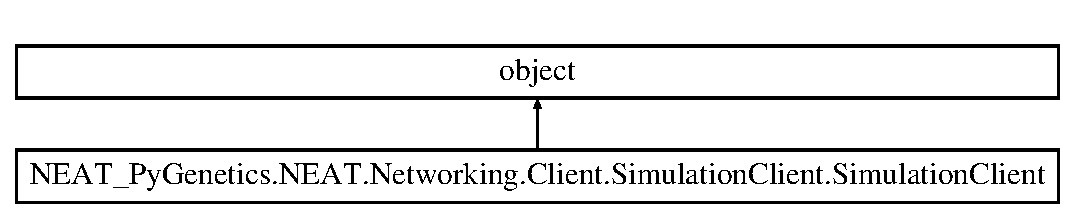
\includegraphics[height=2.000000cm]{classNEAT__PyGenetics_1_1NEAT_1_1Networking_1_1Client_1_1SimulationClient_1_1SimulationClient}
\end{center}
\end{figure}
\subsection*{Public Member Functions}
\begin{DoxyCompactItemize}
\item 
def \hyperlink{classNEAT__PyGenetics_1_1NEAT_1_1Networking_1_1Client_1_1SimulationClient_1_1SimulationClient_a1c778ac890847ec7cf4f2dedab962ce9}{\+\_\+\+\_\+init\+\_\+\+\_\+} (self, server\+\_\+address, server\+\_\+port)
\item 
def \hyperlink{classNEAT__PyGenetics_1_1NEAT_1_1Networking_1_1Client_1_1SimulationClient_1_1SimulationClient_a32f0a2edf3339e2d874bca161516ac18}{announce\+\_\+session} (self, session\+\_\+id, config\+\_\+path=None, block\+\_\+size=1)
\item 
def \hyperlink{classNEAT__PyGenetics_1_1NEAT_1_1Networking_1_1Client_1_1SimulationClient_1_1SimulationClient_ad77ac994b568f19bb7468ebff9332cbc}{get\+\_\+block}
\item 
def \hyperlink{classNEAT__PyGenetics_1_1NEAT_1_1Networking_1_1Client_1_1SimulationClient_1_1SimulationClient_a6cb78ce85e0d06b14c4da1235ca554b0}{set\+\_\+block\+\_\+inputs}
\item 
def \hyperlink{classNEAT__PyGenetics_1_1NEAT_1_1Networking_1_1Client_1_1SimulationClient_1_1SimulationClient_a9d5c043ac1439872cfcbb767e751d586}{get\+\_\+block\+\_\+outputs}
\item 
def \hyperlink{classNEAT__PyGenetics_1_1NEAT_1_1Networking_1_1Client_1_1SimulationClient_1_1SimulationClient_a30dca9ecfedc51b314579100f8fa21d4}{set\+\_\+fitness\+\_\+values}
\item 
def \hyperlink{classNEAT__PyGenetics_1_1NEAT_1_1Networking_1_1Client_1_1SimulationClient_1_1SimulationClient_a8aa37dad9f6092178fd4b08e654829ca}{advance\+\_\+generation} (self)
\item 
def \hyperlink{classNEAT__PyGenetics_1_1NEAT_1_1Networking_1_1Client_1_1SimulationClient_1_1SimulationClient_a2b90544554ffa9c9d884f68c9e4ec01b}{archive\+\_\+session} (self)
\end{DoxyCompactItemize}
\subsection*{Static Public Attributes}
\begin{DoxyCompactItemize}
\item 
\hyperlink{classNEAT__PyGenetics_1_1NEAT_1_1Networking_1_1Client_1_1SimulationClient_1_1SimulationClient_ae492ae862d9d7a5096f16051c4b43cb0}{command}
\item 
\hyperlink{classNEAT__PyGenetics_1_1NEAT_1_1Networking_1_1Client_1_1SimulationClient_1_1SimulationClient_a6a2ac9e9e4603999962e160328eaffce}{response}
\end{DoxyCompactItemize}


\subsection{Constructor \& Destructor Documentation}
\index{N\+E\+A\+T\+\_\+\+Py\+Genetics\+::\+N\+E\+A\+T\+::\+Networking\+::\+Client\+::\+Simulation\+Client\+::\+Simulation\+Client@{N\+E\+A\+T\+\_\+\+Py\+Genetics\+::\+N\+E\+A\+T\+::\+Networking\+::\+Client\+::\+Simulation\+Client\+::\+Simulation\+Client}!\+\_\+\+\_\+init\+\_\+\+\_\+@{\+\_\+\+\_\+init\+\_\+\+\_\+}}
\index{\+\_\+\+\_\+init\+\_\+\+\_\+@{\+\_\+\+\_\+init\+\_\+\+\_\+}!N\+E\+A\+T\+\_\+\+Py\+Genetics\+::\+N\+E\+A\+T\+::\+Networking\+::\+Client\+::\+Simulation\+Client\+::\+Simulation\+Client@{N\+E\+A\+T\+\_\+\+Py\+Genetics\+::\+N\+E\+A\+T\+::\+Networking\+::\+Client\+::\+Simulation\+Client\+::\+Simulation\+Client}}
\subsubsection[{\texorpdfstring{\+\_\+\+\_\+init\+\_\+\+\_\+(self, server\+\_\+address, server\+\_\+port)}{__init__(self, server_address, server_port)}}]{\setlength{\rightskip}{0pt plus 5cm}def N\+E\+A\+T\+\_\+\+Py\+Genetics.\+N\+E\+A\+T.\+Networking.\+Client.\+Simulation\+Client.\+Simulation\+Client.\+\_\+\+\_\+init\+\_\+\+\_\+ (
\begin{DoxyParamCaption}
\item[{}]{self, }
\item[{}]{server\+\_\+address, }
\item[{}]{server\+\_\+port}
\end{DoxyParamCaption}
)}\hypertarget{classNEAT__PyGenetics_1_1NEAT_1_1Networking_1_1Client_1_1SimulationClient_1_1SimulationClient_a1c778ac890847ec7cf4f2dedab962ce9}{}\label{classNEAT__PyGenetics_1_1NEAT_1_1Networking_1_1Client_1_1SimulationClient_1_1SimulationClient_a1c778ac890847ec7cf4f2dedab962ce9}


\subsection{Member Function Documentation}
\index{N\+E\+A\+T\+\_\+\+Py\+Genetics\+::\+N\+E\+A\+T\+::\+Networking\+::\+Client\+::\+Simulation\+Client\+::\+Simulation\+Client@{N\+E\+A\+T\+\_\+\+Py\+Genetics\+::\+N\+E\+A\+T\+::\+Networking\+::\+Client\+::\+Simulation\+Client\+::\+Simulation\+Client}!advance\+\_\+generation@{advance\+\_\+generation}}
\index{advance\+\_\+generation@{advance\+\_\+generation}!N\+E\+A\+T\+\_\+\+Py\+Genetics\+::\+N\+E\+A\+T\+::\+Networking\+::\+Client\+::\+Simulation\+Client\+::\+Simulation\+Client@{N\+E\+A\+T\+\_\+\+Py\+Genetics\+::\+N\+E\+A\+T\+::\+Networking\+::\+Client\+::\+Simulation\+Client\+::\+Simulation\+Client}}
\subsubsection[{\texorpdfstring{advance\+\_\+generation(self)}{advance_generation(self)}}]{\setlength{\rightskip}{0pt plus 5cm}def N\+E\+A\+T\+\_\+\+Py\+Genetics.\+N\+E\+A\+T.\+Networking.\+Client.\+Simulation\+Client.\+Simulation\+Client.\+advance\+\_\+generation (
\begin{DoxyParamCaption}
\item[{}]{self, }
\item[{}]{Advance\+Generation\+Command}
\end{DoxyParamCaption}
)}\hypertarget{classNEAT__PyGenetics_1_1NEAT_1_1Networking_1_1Client_1_1SimulationClient_1_1SimulationClient_a8aa37dad9f6092178fd4b08e654829ca}{}\label{classNEAT__PyGenetics_1_1NEAT_1_1Networking_1_1Client_1_1SimulationClient_1_1SimulationClient_a8aa37dad9f6092178fd4b08e654829ca}
\index{N\+E\+A\+T\+\_\+\+Py\+Genetics\+::\+N\+E\+A\+T\+::\+Networking\+::\+Client\+::\+Simulation\+Client\+::\+Simulation\+Client@{N\+E\+A\+T\+\_\+\+Py\+Genetics\+::\+N\+E\+A\+T\+::\+Networking\+::\+Client\+::\+Simulation\+Client\+::\+Simulation\+Client}!announce\+\_\+session@{announce\+\_\+session}}
\index{announce\+\_\+session@{announce\+\_\+session}!N\+E\+A\+T\+\_\+\+Py\+Genetics\+::\+N\+E\+A\+T\+::\+Networking\+::\+Client\+::\+Simulation\+Client\+::\+Simulation\+Client@{N\+E\+A\+T\+\_\+\+Py\+Genetics\+::\+N\+E\+A\+T\+::\+Networking\+::\+Client\+::\+Simulation\+Client\+::\+Simulation\+Client}}
\subsubsection[{\texorpdfstring{announce\+\_\+session(self, session\+\_\+id, config\+\_\+path=\+None, block\+\_\+size=1)}{announce_session(self, session_id, config_path=None, block_size=1)}}]{\setlength{\rightskip}{0pt plus 5cm}def N\+E\+A\+T\+\_\+\+Py\+Genetics.\+N\+E\+A\+T.\+Networking.\+Client.\+Simulation\+Client.\+Simulation\+Client.\+announce\+\_\+session (
\begin{DoxyParamCaption}
\item[{}]{self, }
\item[{}]{session\+\_\+id, }
\item[{}]{config\+\_\+path = {\ttfamily None}, }
\item[{}]{block\+\_\+size = {\ttfamily 1}}
\end{DoxyParamCaption}
)}\hypertarget{classNEAT__PyGenetics_1_1NEAT_1_1Networking_1_1Client_1_1SimulationClient_1_1SimulationClient_a32f0a2edf3339e2d874bca161516ac18}{}\label{classNEAT__PyGenetics_1_1NEAT_1_1Networking_1_1Client_1_1SimulationClient_1_1SimulationClient_a32f0a2edf3339e2d874bca161516ac18}
\index{N\+E\+A\+T\+\_\+\+Py\+Genetics\+::\+N\+E\+A\+T\+::\+Networking\+::\+Client\+::\+Simulation\+Client\+::\+Simulation\+Client@{N\+E\+A\+T\+\_\+\+Py\+Genetics\+::\+N\+E\+A\+T\+::\+Networking\+::\+Client\+::\+Simulation\+Client\+::\+Simulation\+Client}!archive\+\_\+session@{archive\+\_\+session}}
\index{archive\+\_\+session@{archive\+\_\+session}!N\+E\+A\+T\+\_\+\+Py\+Genetics\+::\+N\+E\+A\+T\+::\+Networking\+::\+Client\+::\+Simulation\+Client\+::\+Simulation\+Client@{N\+E\+A\+T\+\_\+\+Py\+Genetics\+::\+N\+E\+A\+T\+::\+Networking\+::\+Client\+::\+Simulation\+Client\+::\+Simulation\+Client}}
\subsubsection[{\texorpdfstring{archive\+\_\+session(self)}{archive_session(self)}}]{\setlength{\rightskip}{0pt plus 5cm}def N\+E\+A\+T\+\_\+\+Py\+Genetics.\+N\+E\+A\+T.\+Networking.\+Client.\+Simulation\+Client.\+Simulation\+Client.\+archive\+\_\+session (
\begin{DoxyParamCaption}
\item[{}]{self}
\end{DoxyParamCaption}
)}\hypertarget{classNEAT__PyGenetics_1_1NEAT_1_1Networking_1_1Client_1_1SimulationClient_1_1SimulationClient_a2b90544554ffa9c9d884f68c9e4ec01b}{}\label{classNEAT__PyGenetics_1_1NEAT_1_1Networking_1_1Client_1_1SimulationClient_1_1SimulationClient_a2b90544554ffa9c9d884f68c9e4ec01b}
\index{N\+E\+A\+T\+\_\+\+Py\+Genetics\+::\+N\+E\+A\+T\+::\+Networking\+::\+Client\+::\+Simulation\+Client\+::\+Simulation\+Client@{N\+E\+A\+T\+\_\+\+Py\+Genetics\+::\+N\+E\+A\+T\+::\+Networking\+::\+Client\+::\+Simulation\+Client\+::\+Simulation\+Client}!get\+\_\+block@{get\+\_\+block}}
\index{get\+\_\+block@{get\+\_\+block}!N\+E\+A\+T\+\_\+\+Py\+Genetics\+::\+N\+E\+A\+T\+::\+Networking\+::\+Client\+::\+Simulation\+Client\+::\+Simulation\+Client@{N\+E\+A\+T\+\_\+\+Py\+Genetics\+::\+N\+E\+A\+T\+::\+Networking\+::\+Client\+::\+Simulation\+Client\+::\+Simulation\+Client}}
\subsubsection[{\texorpdfstring{get\+\_\+block}{get_block}}]{\setlength{\rightskip}{0pt plus 5cm}def N\+E\+A\+T\+\_\+\+Py\+Genetics.\+N\+E\+A\+T.\+Networking.\+Client.\+Simulation\+Client.\+Simulation\+Client.\+get\+\_\+block (
\begin{DoxyParamCaption}
\item[{}]{self, }
\item[{}]{block\+\_\+id}
\end{DoxyParamCaption}
)}\hypertarget{classNEAT__PyGenetics_1_1NEAT_1_1Networking_1_1Client_1_1SimulationClient_1_1SimulationClient_ad77ac994b568f19bb7468ebff9332cbc}{}\label{classNEAT__PyGenetics_1_1NEAT_1_1Networking_1_1Client_1_1SimulationClient_1_1SimulationClient_ad77ac994b568f19bb7468ebff9332cbc}
\index{N\+E\+A\+T\+\_\+\+Py\+Genetics\+::\+N\+E\+A\+T\+::\+Networking\+::\+Client\+::\+Simulation\+Client\+::\+Simulation\+Client@{N\+E\+A\+T\+\_\+\+Py\+Genetics\+::\+N\+E\+A\+T\+::\+Networking\+::\+Client\+::\+Simulation\+Client\+::\+Simulation\+Client}!get\+\_\+block\+\_\+outputs@{get\+\_\+block\+\_\+outputs}}
\index{get\+\_\+block\+\_\+outputs@{get\+\_\+block\+\_\+outputs}!N\+E\+A\+T\+\_\+\+Py\+Genetics\+::\+N\+E\+A\+T\+::\+Networking\+::\+Client\+::\+Simulation\+Client\+::\+Simulation\+Client@{N\+E\+A\+T\+\_\+\+Py\+Genetics\+::\+N\+E\+A\+T\+::\+Networking\+::\+Client\+::\+Simulation\+Client\+::\+Simulation\+Client}}
\subsubsection[{\texorpdfstring{get\+\_\+block\+\_\+outputs}{get_block_outputs}}]{\setlength{\rightskip}{0pt plus 5cm}def N\+E\+A\+T\+\_\+\+Py\+Genetics.\+N\+E\+A\+T.\+Networking.\+Client.\+Simulation\+Client.\+Simulation\+Client.\+get\+\_\+block\+\_\+outputs (
\begin{DoxyParamCaption}
\item[{}]{self, }
\item[{}]{block\+\_\+id}
\end{DoxyParamCaption}
)}\hypertarget{classNEAT__PyGenetics_1_1NEAT_1_1Networking_1_1Client_1_1SimulationClient_1_1SimulationClient_a9d5c043ac1439872cfcbb767e751d586}{}\label{classNEAT__PyGenetics_1_1NEAT_1_1Networking_1_1Client_1_1SimulationClient_1_1SimulationClient_a9d5c043ac1439872cfcbb767e751d586}
\index{N\+E\+A\+T\+\_\+\+Py\+Genetics\+::\+N\+E\+A\+T\+::\+Networking\+::\+Client\+::\+Simulation\+Client\+::\+Simulation\+Client@{N\+E\+A\+T\+\_\+\+Py\+Genetics\+::\+N\+E\+A\+T\+::\+Networking\+::\+Client\+::\+Simulation\+Client\+::\+Simulation\+Client}!set\+\_\+block\+\_\+inputs@{set\+\_\+block\+\_\+inputs}}
\index{set\+\_\+block\+\_\+inputs@{set\+\_\+block\+\_\+inputs}!N\+E\+A\+T\+\_\+\+Py\+Genetics\+::\+N\+E\+A\+T\+::\+Networking\+::\+Client\+::\+Simulation\+Client\+::\+Simulation\+Client@{N\+E\+A\+T\+\_\+\+Py\+Genetics\+::\+N\+E\+A\+T\+::\+Networking\+::\+Client\+::\+Simulation\+Client\+::\+Simulation\+Client}}
\subsubsection[{\texorpdfstring{set\+\_\+block\+\_\+inputs}{set_block_inputs}}]{\setlength{\rightskip}{0pt plus 5cm}def N\+E\+A\+T\+\_\+\+Py\+Genetics.\+N\+E\+A\+T.\+Networking.\+Client.\+Simulation\+Client.\+Simulation\+Client.\+set\+\_\+block\+\_\+inputs (
\begin{DoxyParamCaption}
\item[{}]{self, }
\item[{}]{inputs}
\end{DoxyParamCaption}
)}\hypertarget{classNEAT__PyGenetics_1_1NEAT_1_1Networking_1_1Client_1_1SimulationClient_1_1SimulationClient_a6cb78ce85e0d06b14c4da1235ca554b0}{}\label{classNEAT__PyGenetics_1_1NEAT_1_1Networking_1_1Client_1_1SimulationClient_1_1SimulationClient_a6cb78ce85e0d06b14c4da1235ca554b0}
\index{N\+E\+A\+T\+\_\+\+Py\+Genetics\+::\+N\+E\+A\+T\+::\+Networking\+::\+Client\+::\+Simulation\+Client\+::\+Simulation\+Client@{N\+E\+A\+T\+\_\+\+Py\+Genetics\+::\+N\+E\+A\+T\+::\+Networking\+::\+Client\+::\+Simulation\+Client\+::\+Simulation\+Client}!set\+\_\+fitness\+\_\+values@{set\+\_\+fitness\+\_\+values}}
\index{set\+\_\+fitness\+\_\+values@{set\+\_\+fitness\+\_\+values}!N\+E\+A\+T\+\_\+\+Py\+Genetics\+::\+N\+E\+A\+T\+::\+Networking\+::\+Client\+::\+Simulation\+Client\+::\+Simulation\+Client@{N\+E\+A\+T\+\_\+\+Py\+Genetics\+::\+N\+E\+A\+T\+::\+Networking\+::\+Client\+::\+Simulation\+Client\+::\+Simulation\+Client}}
\subsubsection[{\texorpdfstring{set\+\_\+fitness\+\_\+values}{set_fitness_values}}]{\setlength{\rightskip}{0pt plus 5cm}def N\+E\+A\+T\+\_\+\+Py\+Genetics.\+N\+E\+A\+T.\+Networking.\+Client.\+Simulation\+Client.\+Simulation\+Client.\+set\+\_\+fitness\+\_\+values (
\begin{DoxyParamCaption}
\item[{}]{self, }
\item[{}]{fitness\+\_\+values}
\end{DoxyParamCaption}
)}\hypertarget{classNEAT__PyGenetics_1_1NEAT_1_1Networking_1_1Client_1_1SimulationClient_1_1SimulationClient_a30dca9ecfedc51b314579100f8fa21d4}{}\label{classNEAT__PyGenetics_1_1NEAT_1_1Networking_1_1Client_1_1SimulationClient_1_1SimulationClient_a30dca9ecfedc51b314579100f8fa21d4}


\subsection{Member Data Documentation}
\index{N\+E\+A\+T\+\_\+\+Py\+Genetics\+::\+N\+E\+A\+T\+::\+Networking\+::\+Client\+::\+Simulation\+Client\+::\+Simulation\+Client@{N\+E\+A\+T\+\_\+\+Py\+Genetics\+::\+N\+E\+A\+T\+::\+Networking\+::\+Client\+::\+Simulation\+Client\+::\+Simulation\+Client}!command@{command}}
\index{command@{command}!N\+E\+A\+T\+\_\+\+Py\+Genetics\+::\+N\+E\+A\+T\+::\+Networking\+::\+Client\+::\+Simulation\+Client\+::\+Simulation\+Client@{N\+E\+A\+T\+\_\+\+Py\+Genetics\+::\+N\+E\+A\+T\+::\+Networking\+::\+Client\+::\+Simulation\+Client\+::\+Simulation\+Client}}
\subsubsection[{\texorpdfstring{command}{command}}]{\setlength{\rightskip}{0pt plus 5cm}N\+E\+A\+T\+\_\+\+Py\+Genetics.\+N\+E\+A\+T.\+Networking.\+Client.\+Simulation\+Client.\+Simulation\+Client.\+command\hspace{0.3cm}{\ttfamily [static]}}\hypertarget{classNEAT__PyGenetics_1_1NEAT_1_1Networking_1_1Client_1_1SimulationClient_1_1SimulationClient_ae492ae862d9d7a5096f16051c4b43cb0}{}\label{classNEAT__PyGenetics_1_1NEAT_1_1Networking_1_1Client_1_1SimulationClient_1_1SimulationClient_ae492ae862d9d7a5096f16051c4b43cb0}
\index{N\+E\+A\+T\+\_\+\+Py\+Genetics\+::\+N\+E\+A\+T\+::\+Networking\+::\+Client\+::\+Simulation\+Client\+::\+Simulation\+Client@{N\+E\+A\+T\+\_\+\+Py\+Genetics\+::\+N\+E\+A\+T\+::\+Networking\+::\+Client\+::\+Simulation\+Client\+::\+Simulation\+Client}!response@{response}}
\index{response@{response}!N\+E\+A\+T\+\_\+\+Py\+Genetics\+::\+N\+E\+A\+T\+::\+Networking\+::\+Client\+::\+Simulation\+Client\+::\+Simulation\+Client@{N\+E\+A\+T\+\_\+\+Py\+Genetics\+::\+N\+E\+A\+T\+::\+Networking\+::\+Client\+::\+Simulation\+Client\+::\+Simulation\+Client}}
\subsubsection[{\texorpdfstring{response}{response}}]{\setlength{\rightskip}{0pt plus 5cm}N\+E\+A\+T\+\_\+\+Py\+Genetics.\+N\+E\+A\+T.\+Networking.\+Client.\+Simulation\+Client.\+Simulation\+Client.\+response\hspace{0.3cm}{\ttfamily [static]}}\hypertarget{classNEAT__PyGenetics_1_1NEAT_1_1Networking_1_1Client_1_1SimulationClient_1_1SimulationClient_a6a2ac9e9e4603999962e160328eaffce}{}\label{classNEAT__PyGenetics_1_1NEAT_1_1Networking_1_1Client_1_1SimulationClient_1_1SimulationClient_a6a2ac9e9e4603999962e160328eaffce}


The documentation for this class was generated from the following file\+:\begin{DoxyCompactItemize}
\item 
N\+E\+A\+T/\+Networking/\+Client/\hyperlink{SimulationClient_8py}{Simulation\+Client.\+py}\end{DoxyCompactItemize}

\hypertarget{classNEAT__PyGenetics_1_1NEAT_1_1Networking_1_1Server_1_1SimulationConnector_1_1SimulationConnector}{}\section{N\+E\+A\+T\+\_\+\+Py\+Genetics.\+N\+E\+A\+T.\+Networking.\+Server.\+Simulation\+Connector.\+Simulation\+Connector Class Reference}
\label{classNEAT__PyGenetics_1_1NEAT_1_1Networking_1_1Server_1_1SimulationConnector_1_1SimulationConnector}\index{N\+E\+A\+T\+\_\+\+Py\+Genetics.\+N\+E\+A\+T.\+Networking.\+Server.\+Simulation\+Connector.\+Simulation\+Connector@{N\+E\+A\+T\+\_\+\+Py\+Genetics.\+N\+E\+A\+T.\+Networking.\+Server.\+Simulation\+Connector.\+Simulation\+Connector}}


A class providing a high-\/level interface to a client connected via the N\+E\+A\+T\+Client.  


Inheritance diagram for N\+E\+A\+T\+\_\+\+Py\+Genetics.\+N\+E\+A\+T.\+Networking.\+Server.\+Simulation\+Connector.\+Simulation\+Connector\+:\begin{figure}[H]
\begin{center}
\leavevmode
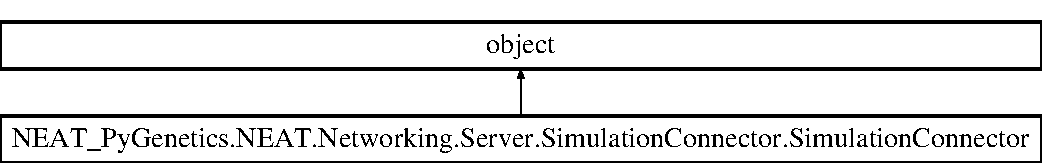
\includegraphics[height=2.000000cm]{classNEAT__PyGenetics_1_1NEAT_1_1Networking_1_1Server_1_1SimulationConnector_1_1SimulationConnector}
\end{center}
\end{figure}
\subsection*{Public Member Functions}
\begin{DoxyCompactItemize}
\item 
def \hyperlink{classNEAT__PyGenetics_1_1NEAT_1_1Networking_1_1Server_1_1SimulationConnector_1_1SimulationConnector_a3efe4fc8a7d68cfd454fbaf0e981bee5}{\+\_\+\+\_\+init\+\_\+\+\_\+} (self)
\item 
def \hyperlink{classNEAT__PyGenetics_1_1NEAT_1_1Networking_1_1Server_1_1SimulationConnector_1_1SimulationConnector_af5849c17a1aa5ef6bc4f9e1f798fe00c}{get\+\_\+session} (self)
\begin{DoxyCompactList}\small\item\em Awaits the Announce\+Session command to be sent by the client. \end{DoxyCompactList}\item 
def \hyperlink{classNEAT__PyGenetics_1_1NEAT_1_1Networking_1_1Server_1_1SimulationConnector_1_1SimulationConnector_a4984c0604704e1808a51050274c7a56e}{send\+\_\+block}
\begin{DoxyCompactList}\small\item\em Awaits the Get\+Block command to be sent by the client and sends the block to the client. \end{DoxyCompactList}\item 
def \hyperlink{classNEAT__PyGenetics_1_1NEAT_1_1Networking_1_1Server_1_1SimulationConnector_1_1SimulationConnector_a193505d0bf3a8dfa0063b7aca22cd84b}{get\+\_\+block\+\_\+inputs}
\begin{DoxyCompactList}\small\item\em Awaits the Set\+Inputs command to be sent by the client. \end{DoxyCompactList}\item 
def \hyperlink{classNEAT__PyGenetics_1_1NEAT_1_1Networking_1_1Server_1_1SimulationConnector_1_1SimulationConnector_a82d0ed025654632c25d2241aef9024cc}{send\+\_\+block\+\_\+outputs}
\begin{DoxyCompactList}\small\item\em Awaits the Get\+Outputs command to be sent by the client and sends the outputs for the previously received inputs back to the client. \end{DoxyCompactList}\item 
def \hyperlink{classNEAT__PyGenetics_1_1NEAT_1_1Networking_1_1Server_1_1SimulationConnector_1_1SimulationConnector_af63e36b9eb1e3dcc9d58e437d251cc35}{get\+\_\+fitness\+\_\+values}
\begin{DoxyCompactList}\small\item\em Awaits the Set\+Fitness\+Values command to be sent by the client. \end{DoxyCompactList}\item 
def \hyperlink{classNEAT__PyGenetics_1_1NEAT_1_1Networking_1_1Server_1_1SimulationConnector_1_1SimulationConnector_a5a07ea6d6971102b7dbe65e8fbaeb2c6}{get\+\_\+advance\+\_\+generation} (self)
\begin{DoxyCompactList}\small\item\em Awaits the Advance\+Generation command to be sent by the client. \end{DoxyCompactList}\end{DoxyCompactItemize}
\subsection*{Static Public Attributes}
\begin{DoxyCompactItemize}
\item 
\hyperlink{classNEAT__PyGenetics_1_1NEAT_1_1Networking_1_1Server_1_1SimulationConnector_1_1SimulationConnector_a2ee895f0adc1c5612da513e76337a2a1}{command}
\item 
\hyperlink{classNEAT__PyGenetics_1_1NEAT_1_1Networking_1_1Server_1_1SimulationConnector_1_1SimulationConnector_a382935d414f40fe1f061eb2599aaee45}{acknowledged}
\item 
\hyperlink{classNEAT__PyGenetics_1_1NEAT_1_1Networking_1_1Server_1_1SimulationConnector_1_1SimulationConnector_a192917886950be80d6b617d89741272e}{result}
\item 
\hyperlink{classNEAT__PyGenetics_1_1NEAT_1_1Networking_1_1Server_1_1SimulationConnector_1_1SimulationConnector_acf2ca405ae294326df8c2ef7b32d7024}{block\+\_\+to\+\_\+send}
\item 
\hyperlink{classNEAT__PyGenetics_1_1NEAT_1_1Networking_1_1Server_1_1SimulationConnector_1_1SimulationConnector_a09ae391da51cbab362309cde45eee5a4}{get\+\_\+command}
\item 
\hyperlink{classNEAT__PyGenetics_1_1NEAT_1_1Networking_1_1Server_1_1SimulationConnector_1_1SimulationConnector_ae984255e91818c23a045b807d373bf1b}{set\+\_\+command}
\end{DoxyCompactItemize}


\subsection{Detailed Description}
A class providing a high-\/level interface to a client connected via the N\+E\+A\+T\+Client. 

It receives commands from \hyperlink{namespaceNEAT__PyGenetics_1_1NEAT_1_1Networking_1_1Server_1_1NEATServer}{N\+E\+A\+T\+Server}\textquotesingle{}s message queue und responds to them. When a function from \hyperlink{classNEAT__PyGenetics_1_1NEAT_1_1Networking_1_1Server_1_1SimulationConnector_1_1SimulationConnector}{Simulation\+Connector} is called, the client is expected to have sent a certain command (if there are no commands in the message queue, the \hyperlink{namespaceNEAT__PyGenetics_1_1NEAT_1_1Networking_1_1Server}{Server} will wait for the next command to be received). If the client has sent another command, or a command where the expected parameters are not present, Network\+Protocol\+Exception will be raised. 

\subsection{Constructor \& Destructor Documentation}
\index{N\+E\+A\+T\+\_\+\+Py\+Genetics\+::\+N\+E\+A\+T\+::\+Networking\+::\+Server\+::\+Simulation\+Connector\+::\+Simulation\+Connector@{N\+E\+A\+T\+\_\+\+Py\+Genetics\+::\+N\+E\+A\+T\+::\+Networking\+::\+Server\+::\+Simulation\+Connector\+::\+Simulation\+Connector}!\+\_\+\+\_\+init\+\_\+\+\_\+@{\+\_\+\+\_\+init\+\_\+\+\_\+}}
\index{\+\_\+\+\_\+init\+\_\+\+\_\+@{\+\_\+\+\_\+init\+\_\+\+\_\+}!N\+E\+A\+T\+\_\+\+Py\+Genetics\+::\+N\+E\+A\+T\+::\+Networking\+::\+Server\+::\+Simulation\+Connector\+::\+Simulation\+Connector@{N\+E\+A\+T\+\_\+\+Py\+Genetics\+::\+N\+E\+A\+T\+::\+Networking\+::\+Server\+::\+Simulation\+Connector\+::\+Simulation\+Connector}}
\subsubsection[{\texorpdfstring{\+\_\+\+\_\+init\+\_\+\+\_\+(self)}{__init__(self)}}]{\setlength{\rightskip}{0pt plus 5cm}def N\+E\+A\+T\+\_\+\+Py\+Genetics.\+N\+E\+A\+T.\+Networking.\+Server.\+Simulation\+Connector.\+Simulation\+Connector.\+\_\+\+\_\+init\+\_\+\+\_\+ (
\begin{DoxyParamCaption}
\item[{}]{self, }
\item[{}]{None}
\end{DoxyParamCaption}
)}\hypertarget{classNEAT__PyGenetics_1_1NEAT_1_1Networking_1_1Server_1_1SimulationConnector_1_1SimulationConnector_a3efe4fc8a7d68cfd454fbaf0e981bee5}{}\label{classNEAT__PyGenetics_1_1NEAT_1_1Networking_1_1Server_1_1SimulationConnector_1_1SimulationConnector_a3efe4fc8a7d68cfd454fbaf0e981bee5}


\subsection{Member Function Documentation}
\index{N\+E\+A\+T\+\_\+\+Py\+Genetics\+::\+N\+E\+A\+T\+::\+Networking\+::\+Server\+::\+Simulation\+Connector\+::\+Simulation\+Connector@{N\+E\+A\+T\+\_\+\+Py\+Genetics\+::\+N\+E\+A\+T\+::\+Networking\+::\+Server\+::\+Simulation\+Connector\+::\+Simulation\+Connector}!get\+\_\+advance\+\_\+generation@{get\+\_\+advance\+\_\+generation}}
\index{get\+\_\+advance\+\_\+generation@{get\+\_\+advance\+\_\+generation}!N\+E\+A\+T\+\_\+\+Py\+Genetics\+::\+N\+E\+A\+T\+::\+Networking\+::\+Server\+::\+Simulation\+Connector\+::\+Simulation\+Connector@{N\+E\+A\+T\+\_\+\+Py\+Genetics\+::\+N\+E\+A\+T\+::\+Networking\+::\+Server\+::\+Simulation\+Connector\+::\+Simulation\+Connector}}
\subsubsection[{\texorpdfstring{get\+\_\+advance\+\_\+generation(self)}{get_advance_generation(self)}}]{\setlength{\rightskip}{0pt plus 5cm}def N\+E\+A\+T\+\_\+\+Py\+Genetics.\+N\+E\+A\+T.\+Networking.\+Server.\+Simulation\+Connector.\+Simulation\+Connector.\+get\+\_\+advance\+\_\+generation (
\begin{DoxyParamCaption}
\item[{}]{self, }
\item[{}]{bool}
\end{DoxyParamCaption}
)}\hypertarget{classNEAT__PyGenetics_1_1NEAT_1_1Networking_1_1Server_1_1SimulationConnector_1_1SimulationConnector_a5a07ea6d6971102b7dbe65e8fbaeb2c6}{}\label{classNEAT__PyGenetics_1_1NEAT_1_1Networking_1_1Server_1_1SimulationConnector_1_1SimulationConnector_a5a07ea6d6971102b7dbe65e8fbaeb2c6}


Awaits the Advance\+Generation command to be sent by the client. 

\+:return\+: A bool indicating whether the next generation should be calculated by \hyperlink{namespaceNEAT__PyGenetics_1_1NEAT}{N\+E\+AT} (True) or the current session should be archived (False). \index{N\+E\+A\+T\+\_\+\+Py\+Genetics\+::\+N\+E\+A\+T\+::\+Networking\+::\+Server\+::\+Simulation\+Connector\+::\+Simulation\+Connector@{N\+E\+A\+T\+\_\+\+Py\+Genetics\+::\+N\+E\+A\+T\+::\+Networking\+::\+Server\+::\+Simulation\+Connector\+::\+Simulation\+Connector}!get\+\_\+block\+\_\+inputs@{get\+\_\+block\+\_\+inputs}}
\index{get\+\_\+block\+\_\+inputs@{get\+\_\+block\+\_\+inputs}!N\+E\+A\+T\+\_\+\+Py\+Genetics\+::\+N\+E\+A\+T\+::\+Networking\+::\+Server\+::\+Simulation\+Connector\+::\+Simulation\+Connector@{N\+E\+A\+T\+\_\+\+Py\+Genetics\+::\+N\+E\+A\+T\+::\+Networking\+::\+Server\+::\+Simulation\+Connector\+::\+Simulation\+Connector}}
\subsubsection[{\texorpdfstring{get\+\_\+block\+\_\+inputs}{get_block_inputs}}]{\setlength{\rightskip}{0pt plus 5cm}def N\+E\+A\+T\+\_\+\+Py\+Genetics.\+N\+E\+A\+T.\+Networking.\+Server.\+Simulation\+Connector.\+Simulation\+Connector.\+get\+\_\+block\+\_\+inputs (
\begin{DoxyParamCaption}
\item[{}]{self, }
\item[{}]{block\+\_\+id}
\end{DoxyParamCaption}
)}\hypertarget{classNEAT__PyGenetics_1_1NEAT_1_1Networking_1_1Server_1_1SimulationConnector_1_1SimulationConnector_a193505d0bf3a8dfa0063b7aca22cd84b}{}\label{classNEAT__PyGenetics_1_1NEAT_1_1Networking_1_1Server_1_1SimulationConnector_1_1SimulationConnector_a193505d0bf3a8dfa0063b7aca22cd84b}


Awaits the Set\+Inputs command to be sent by the client. 

\+:param block\+\_\+id\+: The id of the block whose inputs should by received \+:return\+: The received inputs as Dictionary of genome\+\_\+id\+: Dict\mbox{[}input\+\_\+label\+: input\+\_\+value\mbox{]} \index{N\+E\+A\+T\+\_\+\+Py\+Genetics\+::\+N\+E\+A\+T\+::\+Networking\+::\+Server\+::\+Simulation\+Connector\+::\+Simulation\+Connector@{N\+E\+A\+T\+\_\+\+Py\+Genetics\+::\+N\+E\+A\+T\+::\+Networking\+::\+Server\+::\+Simulation\+Connector\+::\+Simulation\+Connector}!get\+\_\+fitness\+\_\+values@{get\+\_\+fitness\+\_\+values}}
\index{get\+\_\+fitness\+\_\+values@{get\+\_\+fitness\+\_\+values}!N\+E\+A\+T\+\_\+\+Py\+Genetics\+::\+N\+E\+A\+T\+::\+Networking\+::\+Server\+::\+Simulation\+Connector\+::\+Simulation\+Connector@{N\+E\+A\+T\+\_\+\+Py\+Genetics\+::\+N\+E\+A\+T\+::\+Networking\+::\+Server\+::\+Simulation\+Connector\+::\+Simulation\+Connector}}
\subsubsection[{\texorpdfstring{get\+\_\+fitness\+\_\+values}{get_fitness_values}}]{\setlength{\rightskip}{0pt plus 5cm}def N\+E\+A\+T\+\_\+\+Py\+Genetics.\+N\+E\+A\+T.\+Networking.\+Server.\+Simulation\+Connector.\+Simulation\+Connector.\+get\+\_\+fitness\+\_\+values (
\begin{DoxyParamCaption}
\item[{}]{self, }
\item[{}]{block\+\_\+id}
\end{DoxyParamCaption}
)}\hypertarget{classNEAT__PyGenetics_1_1NEAT_1_1Networking_1_1Server_1_1SimulationConnector_1_1SimulationConnector_af63e36b9eb1e3dcc9d58e437d251cc35}{}\label{classNEAT__PyGenetics_1_1NEAT_1_1Networking_1_1Server_1_1SimulationConnector_1_1SimulationConnector_af63e36b9eb1e3dcc9d58e437d251cc35}


Awaits the Set\+Fitness\+Values command to be sent by the client. 

\+:param block\+\_\+id\+: The id of the block whose fitness values should be received \+:return\+: The received fitness values as dictionary of genome\+\_\+id\+: fitness\+\_\+value \index{N\+E\+A\+T\+\_\+\+Py\+Genetics\+::\+N\+E\+A\+T\+::\+Networking\+::\+Server\+::\+Simulation\+Connector\+::\+Simulation\+Connector@{N\+E\+A\+T\+\_\+\+Py\+Genetics\+::\+N\+E\+A\+T\+::\+Networking\+::\+Server\+::\+Simulation\+Connector\+::\+Simulation\+Connector}!get\+\_\+session@{get\+\_\+session}}
\index{get\+\_\+session@{get\+\_\+session}!N\+E\+A\+T\+\_\+\+Py\+Genetics\+::\+N\+E\+A\+T\+::\+Networking\+::\+Server\+::\+Simulation\+Connector\+::\+Simulation\+Connector@{N\+E\+A\+T\+\_\+\+Py\+Genetics\+::\+N\+E\+A\+T\+::\+Networking\+::\+Server\+::\+Simulation\+Connector\+::\+Simulation\+Connector}}
\subsubsection[{\texorpdfstring{get\+\_\+session(self)}{get_session(self)}}]{\setlength{\rightskip}{0pt plus 5cm}def N\+E\+A\+T\+\_\+\+Py\+Genetics.\+N\+E\+A\+T.\+Networking.\+Server.\+Simulation\+Connector.\+Simulation\+Connector.\+get\+\_\+session (
\begin{DoxyParamCaption}
\item[{}]{self, }
\item[{}]{Dict, }
\item[{}]{str, }
\item[{}]{object}
\end{DoxyParamCaption}
)}\hypertarget{classNEAT__PyGenetics_1_1NEAT_1_1Networking_1_1Server_1_1SimulationConnector_1_1SimulationConnector_af5849c17a1aa5ef6bc4f9e1f798fe00c}{}\label{classNEAT__PyGenetics_1_1NEAT_1_1Networking_1_1Server_1_1SimulationConnector_1_1SimulationConnector_af5849c17a1aa5ef6bc4f9e1f798fe00c}


Awaits the Announce\+Session command to be sent by the client. 

\+:return\+: The session parameters for the new simulation session \index{N\+E\+A\+T\+\_\+\+Py\+Genetics\+::\+N\+E\+A\+T\+::\+Networking\+::\+Server\+::\+Simulation\+Connector\+::\+Simulation\+Connector@{N\+E\+A\+T\+\_\+\+Py\+Genetics\+::\+N\+E\+A\+T\+::\+Networking\+::\+Server\+::\+Simulation\+Connector\+::\+Simulation\+Connector}!send\+\_\+block@{send\+\_\+block}}
\index{send\+\_\+block@{send\+\_\+block}!N\+E\+A\+T\+\_\+\+Py\+Genetics\+::\+N\+E\+A\+T\+::\+Networking\+::\+Server\+::\+Simulation\+Connector\+::\+Simulation\+Connector@{N\+E\+A\+T\+\_\+\+Py\+Genetics\+::\+N\+E\+A\+T\+::\+Networking\+::\+Server\+::\+Simulation\+Connector\+::\+Simulation\+Connector}}
\subsubsection[{\texorpdfstring{send\+\_\+block}{send_block}}]{\setlength{\rightskip}{0pt plus 5cm}def N\+E\+A\+T\+\_\+\+Py\+Genetics.\+N\+E\+A\+T.\+Networking.\+Server.\+Simulation\+Connector.\+Simulation\+Connector.\+send\+\_\+block (
\begin{DoxyParamCaption}
\item[{}]{self, }
\item[{}]{block}
\end{DoxyParamCaption}
)}\hypertarget{classNEAT__PyGenetics_1_1NEAT_1_1Networking_1_1Server_1_1SimulationConnector_1_1SimulationConnector_a4984c0604704e1808a51050274c7a56e}{}\label{classNEAT__PyGenetics_1_1NEAT_1_1Networking_1_1Server_1_1SimulationConnector_1_1SimulationConnector_a4984c0604704e1808a51050274c7a56e}


Awaits the Get\+Block command to be sent by the client and sends the block to the client. 

\+:param block\+: The List of Storage\+Genomes to be sent to the client \+:param block\+\_\+id\+: The id (0 -\/ block\+\_\+count) of the block to be sent \+:return\+: None \index{N\+E\+A\+T\+\_\+\+Py\+Genetics\+::\+N\+E\+A\+T\+::\+Networking\+::\+Server\+::\+Simulation\+Connector\+::\+Simulation\+Connector@{N\+E\+A\+T\+\_\+\+Py\+Genetics\+::\+N\+E\+A\+T\+::\+Networking\+::\+Server\+::\+Simulation\+Connector\+::\+Simulation\+Connector}!send\+\_\+block\+\_\+outputs@{send\+\_\+block\+\_\+outputs}}
\index{send\+\_\+block\+\_\+outputs@{send\+\_\+block\+\_\+outputs}!N\+E\+A\+T\+\_\+\+Py\+Genetics\+::\+N\+E\+A\+T\+::\+Networking\+::\+Server\+::\+Simulation\+Connector\+::\+Simulation\+Connector@{N\+E\+A\+T\+\_\+\+Py\+Genetics\+::\+N\+E\+A\+T\+::\+Networking\+::\+Server\+::\+Simulation\+Connector\+::\+Simulation\+Connector}}
\subsubsection[{\texorpdfstring{send\+\_\+block\+\_\+outputs}{send_block_outputs}}]{\setlength{\rightskip}{0pt plus 5cm}def N\+E\+A\+T\+\_\+\+Py\+Genetics.\+N\+E\+A\+T.\+Networking.\+Server.\+Simulation\+Connector.\+Simulation\+Connector.\+send\+\_\+block\+\_\+outputs (
\begin{DoxyParamCaption}
\item[{}]{self, }
\item[{}]{outputs}
\end{DoxyParamCaption}
)}\hypertarget{classNEAT__PyGenetics_1_1NEAT_1_1Networking_1_1Server_1_1SimulationConnector_1_1SimulationConnector_a82d0ed025654632c25d2241aef9024cc}{}\label{classNEAT__PyGenetics_1_1NEAT_1_1Networking_1_1Server_1_1SimulationConnector_1_1SimulationConnector_a82d0ed025654632c25d2241aef9024cc}


Awaits the Get\+Outputs command to be sent by the client and sends the outputs for the previously received inputs back to the client. 

\+:param outputs\+: The output values as dictionary of genome\+\_\+id\+: Dict\mbox{[}output\+\_\+label\+: output\+\_\+value\mbox{]} \+:param block\+\_\+id\+: The od of the block whose inputs should be sent \+:return\+: None 

\subsection{Member Data Documentation}
\index{N\+E\+A\+T\+\_\+\+Py\+Genetics\+::\+N\+E\+A\+T\+::\+Networking\+::\+Server\+::\+Simulation\+Connector\+::\+Simulation\+Connector@{N\+E\+A\+T\+\_\+\+Py\+Genetics\+::\+N\+E\+A\+T\+::\+Networking\+::\+Server\+::\+Simulation\+Connector\+::\+Simulation\+Connector}!acknowledged@{acknowledged}}
\index{acknowledged@{acknowledged}!N\+E\+A\+T\+\_\+\+Py\+Genetics\+::\+N\+E\+A\+T\+::\+Networking\+::\+Server\+::\+Simulation\+Connector\+::\+Simulation\+Connector@{N\+E\+A\+T\+\_\+\+Py\+Genetics\+::\+N\+E\+A\+T\+::\+Networking\+::\+Server\+::\+Simulation\+Connector\+::\+Simulation\+Connector}}
\subsubsection[{\texorpdfstring{acknowledged}{acknowledged}}]{\setlength{\rightskip}{0pt plus 5cm}N\+E\+A\+T\+\_\+\+Py\+Genetics.\+N\+E\+A\+T.\+Networking.\+Server.\+Simulation\+Connector.\+Simulation\+Connector.\+acknowledged\hspace{0.3cm}{\ttfamily [static]}}\hypertarget{classNEAT__PyGenetics_1_1NEAT_1_1Networking_1_1Server_1_1SimulationConnector_1_1SimulationConnector_a382935d414f40fe1f061eb2599aaee45}{}\label{classNEAT__PyGenetics_1_1NEAT_1_1Networking_1_1Server_1_1SimulationConnector_1_1SimulationConnector_a382935d414f40fe1f061eb2599aaee45}
\index{N\+E\+A\+T\+\_\+\+Py\+Genetics\+::\+N\+E\+A\+T\+::\+Networking\+::\+Server\+::\+Simulation\+Connector\+::\+Simulation\+Connector@{N\+E\+A\+T\+\_\+\+Py\+Genetics\+::\+N\+E\+A\+T\+::\+Networking\+::\+Server\+::\+Simulation\+Connector\+::\+Simulation\+Connector}!block\+\_\+to\+\_\+send@{block\+\_\+to\+\_\+send}}
\index{block\+\_\+to\+\_\+send@{block\+\_\+to\+\_\+send}!N\+E\+A\+T\+\_\+\+Py\+Genetics\+::\+N\+E\+A\+T\+::\+Networking\+::\+Server\+::\+Simulation\+Connector\+::\+Simulation\+Connector@{N\+E\+A\+T\+\_\+\+Py\+Genetics\+::\+N\+E\+A\+T\+::\+Networking\+::\+Server\+::\+Simulation\+Connector\+::\+Simulation\+Connector}}
\subsubsection[{\texorpdfstring{block\+\_\+to\+\_\+send}{block_to_send}}]{\setlength{\rightskip}{0pt plus 5cm}N\+E\+A\+T\+\_\+\+Py\+Genetics.\+N\+E\+A\+T.\+Networking.\+Server.\+Simulation\+Connector.\+Simulation\+Connector.\+block\+\_\+to\+\_\+send\hspace{0.3cm}{\ttfamily [static]}}\hypertarget{classNEAT__PyGenetics_1_1NEAT_1_1Networking_1_1Server_1_1SimulationConnector_1_1SimulationConnector_acf2ca405ae294326df8c2ef7b32d7024}{}\label{classNEAT__PyGenetics_1_1NEAT_1_1Networking_1_1Server_1_1SimulationConnector_1_1SimulationConnector_acf2ca405ae294326df8c2ef7b32d7024}
\index{N\+E\+A\+T\+\_\+\+Py\+Genetics\+::\+N\+E\+A\+T\+::\+Networking\+::\+Server\+::\+Simulation\+Connector\+::\+Simulation\+Connector@{N\+E\+A\+T\+\_\+\+Py\+Genetics\+::\+N\+E\+A\+T\+::\+Networking\+::\+Server\+::\+Simulation\+Connector\+::\+Simulation\+Connector}!command@{command}}
\index{command@{command}!N\+E\+A\+T\+\_\+\+Py\+Genetics\+::\+N\+E\+A\+T\+::\+Networking\+::\+Server\+::\+Simulation\+Connector\+::\+Simulation\+Connector@{N\+E\+A\+T\+\_\+\+Py\+Genetics\+::\+N\+E\+A\+T\+::\+Networking\+::\+Server\+::\+Simulation\+Connector\+::\+Simulation\+Connector}}
\subsubsection[{\texorpdfstring{command}{command}}]{\setlength{\rightskip}{0pt plus 5cm}N\+E\+A\+T\+\_\+\+Py\+Genetics.\+N\+E\+A\+T.\+Networking.\+Server.\+Simulation\+Connector.\+Simulation\+Connector.\+command\hspace{0.3cm}{\ttfamily [static]}}\hypertarget{classNEAT__PyGenetics_1_1NEAT_1_1Networking_1_1Server_1_1SimulationConnector_1_1SimulationConnector_a2ee895f0adc1c5612da513e76337a2a1}{}\label{classNEAT__PyGenetics_1_1NEAT_1_1Networking_1_1Server_1_1SimulationConnector_1_1SimulationConnector_a2ee895f0adc1c5612da513e76337a2a1}
\index{N\+E\+A\+T\+\_\+\+Py\+Genetics\+::\+N\+E\+A\+T\+::\+Networking\+::\+Server\+::\+Simulation\+Connector\+::\+Simulation\+Connector@{N\+E\+A\+T\+\_\+\+Py\+Genetics\+::\+N\+E\+A\+T\+::\+Networking\+::\+Server\+::\+Simulation\+Connector\+::\+Simulation\+Connector}!get\+\_\+command@{get\+\_\+command}}
\index{get\+\_\+command@{get\+\_\+command}!N\+E\+A\+T\+\_\+\+Py\+Genetics\+::\+N\+E\+A\+T\+::\+Networking\+::\+Server\+::\+Simulation\+Connector\+::\+Simulation\+Connector@{N\+E\+A\+T\+\_\+\+Py\+Genetics\+::\+N\+E\+A\+T\+::\+Networking\+::\+Server\+::\+Simulation\+Connector\+::\+Simulation\+Connector}}
\subsubsection[{\texorpdfstring{get\+\_\+command}{get_command}}]{\setlength{\rightskip}{0pt plus 5cm}N\+E\+A\+T\+\_\+\+Py\+Genetics.\+N\+E\+A\+T.\+Networking.\+Server.\+Simulation\+Connector.\+Simulation\+Connector.\+get\+\_\+command\hspace{0.3cm}{\ttfamily [static]}}\hypertarget{classNEAT__PyGenetics_1_1NEAT_1_1Networking_1_1Server_1_1SimulationConnector_1_1SimulationConnector_a09ae391da51cbab362309cde45eee5a4}{}\label{classNEAT__PyGenetics_1_1NEAT_1_1Networking_1_1Server_1_1SimulationConnector_1_1SimulationConnector_a09ae391da51cbab362309cde45eee5a4}
\index{N\+E\+A\+T\+\_\+\+Py\+Genetics\+::\+N\+E\+A\+T\+::\+Networking\+::\+Server\+::\+Simulation\+Connector\+::\+Simulation\+Connector@{N\+E\+A\+T\+\_\+\+Py\+Genetics\+::\+N\+E\+A\+T\+::\+Networking\+::\+Server\+::\+Simulation\+Connector\+::\+Simulation\+Connector}!result@{result}}
\index{result@{result}!N\+E\+A\+T\+\_\+\+Py\+Genetics\+::\+N\+E\+A\+T\+::\+Networking\+::\+Server\+::\+Simulation\+Connector\+::\+Simulation\+Connector@{N\+E\+A\+T\+\_\+\+Py\+Genetics\+::\+N\+E\+A\+T\+::\+Networking\+::\+Server\+::\+Simulation\+Connector\+::\+Simulation\+Connector}}
\subsubsection[{\texorpdfstring{result}{result}}]{\setlength{\rightskip}{0pt plus 5cm}N\+E\+A\+T\+\_\+\+Py\+Genetics.\+N\+E\+A\+T.\+Networking.\+Server.\+Simulation\+Connector.\+Simulation\+Connector.\+result\hspace{0.3cm}{\ttfamily [static]}}\hypertarget{classNEAT__PyGenetics_1_1NEAT_1_1Networking_1_1Server_1_1SimulationConnector_1_1SimulationConnector_a192917886950be80d6b617d89741272e}{}\label{classNEAT__PyGenetics_1_1NEAT_1_1Networking_1_1Server_1_1SimulationConnector_1_1SimulationConnector_a192917886950be80d6b617d89741272e}
\index{N\+E\+A\+T\+\_\+\+Py\+Genetics\+::\+N\+E\+A\+T\+::\+Networking\+::\+Server\+::\+Simulation\+Connector\+::\+Simulation\+Connector@{N\+E\+A\+T\+\_\+\+Py\+Genetics\+::\+N\+E\+A\+T\+::\+Networking\+::\+Server\+::\+Simulation\+Connector\+::\+Simulation\+Connector}!set\+\_\+command@{set\+\_\+command}}
\index{set\+\_\+command@{set\+\_\+command}!N\+E\+A\+T\+\_\+\+Py\+Genetics\+::\+N\+E\+A\+T\+::\+Networking\+::\+Server\+::\+Simulation\+Connector\+::\+Simulation\+Connector@{N\+E\+A\+T\+\_\+\+Py\+Genetics\+::\+N\+E\+A\+T\+::\+Networking\+::\+Server\+::\+Simulation\+Connector\+::\+Simulation\+Connector}}
\subsubsection[{\texorpdfstring{set\+\_\+command}{set_command}}]{\setlength{\rightskip}{0pt plus 5cm}N\+E\+A\+T\+\_\+\+Py\+Genetics.\+N\+E\+A\+T.\+Networking.\+Server.\+Simulation\+Connector.\+Simulation\+Connector.\+set\+\_\+command\hspace{0.3cm}{\ttfamily [static]}}\hypertarget{classNEAT__PyGenetics_1_1NEAT_1_1Networking_1_1Server_1_1SimulationConnector_1_1SimulationConnector_ae984255e91818c23a045b807d373bf1b}{}\label{classNEAT__PyGenetics_1_1NEAT_1_1Networking_1_1Server_1_1SimulationConnector_1_1SimulationConnector_ae984255e91818c23a045b807d373bf1b}


The documentation for this class was generated from the following file\+:\begin{DoxyCompactItemize}
\item 
N\+E\+A\+T/\+Networking/\+Server/\hyperlink{SimulationConnector_8py}{Simulation\+Connector.\+py}\end{DoxyCompactItemize}

\hypertarget{classNEAT__PyGenetics_1_1NEAT_1_1GenomeStructures_1_1SimulationStructure_1_1SimulationGenome_1_1SimulationGenome}{}\section{N\+E\+A\+T\+\_\+\+Py\+Genetics.\+N\+E\+A\+T.\+Genome\+Structures.\+Simulation\+Structure.\+Simulation\+Genome.\+Simulation\+Genome Class Reference}
\label{classNEAT__PyGenetics_1_1NEAT_1_1GenomeStructures_1_1SimulationStructure_1_1SimulationGenome_1_1SimulationGenome}\index{N\+E\+A\+T\+\_\+\+Py\+Genetics.\+N\+E\+A\+T.\+Genome\+Structures.\+Simulation\+Structure.\+Simulation\+Genome.\+Simulation\+Genome@{N\+E\+A\+T\+\_\+\+Py\+Genetics.\+N\+E\+A\+T.\+Genome\+Structures.\+Simulation\+Structure.\+Simulation\+Genome.\+Simulation\+Genome}}
Inheritance diagram for N\+E\+A\+T\+\_\+\+Py\+Genetics.\+N\+E\+A\+T.\+Genome\+Structures.\+Simulation\+Structure.\+Simulation\+Genome.\+Simulation\+Genome\+:\begin{figure}[H]
\begin{center}
\leavevmode
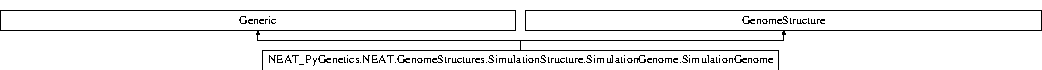
\includegraphics[height=0.939597cm]{classNEAT__PyGenetics_1_1NEAT_1_1GenomeStructures_1_1SimulationStructure_1_1SimulationGenome_1_1SimulationGenome}
\end{center}
\end{figure}
\subsection*{Public Member Functions}
\begin{DoxyCompactItemize}
\item 
def \hyperlink{classNEAT__PyGenetics_1_1NEAT_1_1GenomeStructures_1_1SimulationStructure_1_1SimulationGenome_1_1SimulationGenome_a9e3d21a710e6b90ca8d6332fbdc8faa2}{\+\_\+\+\_\+init\+\_\+\+\_\+}
\item 
def \hyperlink{classNEAT__PyGenetics_1_1NEAT_1_1GenomeStructures_1_1SimulationStructure_1_1SimulationGenome_1_1SimulationGenome_af8bbfbec0e15a55d7a889ba9859f034a}{output} (self)
\begin{DoxyCompactList}\small\item\em \+:return\+: Dict of the output nodes\textquotesingle{} values of the form label\+:value \end{DoxyCompactList}\item 
def \hyperlink{classNEAT__PyGenetics_1_1NEAT_1_1GenomeStructures_1_1SimulationStructure_1_1SimulationGenome_1_1SimulationGenome_ae35fc2d42a8f79cf1cf7cf65b40910b6}{calculate\+\_\+step}
\end{DoxyCompactItemize}
\subsection*{Static Public Attributes}
\begin{DoxyCompactItemize}
\item 
\hyperlink{classNEAT__PyGenetics_1_1NEAT_1_1GenomeStructures_1_1SimulationStructure_1_1SimulationGenome_1_1SimulationGenome_aa650dc24f64c63322197e5eabd879453}{cycle\+\_\+nodes}
\item 
\hyperlink{classNEAT__PyGenetics_1_1NEAT_1_1GenomeStructures_1_1SimulationStructure_1_1SimulationGenome_1_1SimulationGenome_a66d27e8ed15eb8473d63728d6fa046fe}{hidden\+\_\+layer}
\item 
\hyperlink{classNEAT__PyGenetics_1_1NEAT_1_1GenomeStructures_1_1SimulationStructure_1_1SimulationGenome_1_1SimulationGenome_a246a2949988d817f3ba2e5a27ce0cb26}{closes\+\_\+circle}
\item 
\hyperlink{classNEAT__PyGenetics_1_1NEAT_1_1GenomeStructures_1_1SimulationStructure_1_1SimulationGenome_1_1SimulationGenome_ac4b5b345246df8c26156052e19d88dc3}{source}
\item 
\hyperlink{classNEAT__PyGenetics_1_1NEAT_1_1GenomeStructures_1_1SimulationStructure_1_1SimulationGenome_1_1SimulationGenome_ac175e1e9455296d28d7486373e2546c7}{target}
\item 
\hyperlink{classNEAT__PyGenetics_1_1NEAT_1_1GenomeStructures_1_1SimulationStructure_1_1SimulationGenome_1_1SimulationGenome_a27b218236fdf7a6526bdddef382a38e9}{value}
\end{DoxyCompactItemize}


\subsection{Constructor \& Destructor Documentation}
\index{N\+E\+A\+T\+\_\+\+Py\+Genetics\+::\+N\+E\+A\+T\+::\+Genome\+Structures\+::\+Simulation\+Structure\+::\+Simulation\+Genome\+::\+Simulation\+Genome@{N\+E\+A\+T\+\_\+\+Py\+Genetics\+::\+N\+E\+A\+T\+::\+Genome\+Structures\+::\+Simulation\+Structure\+::\+Simulation\+Genome\+::\+Simulation\+Genome}!\+\_\+\+\_\+init\+\_\+\+\_\+@{\+\_\+\+\_\+init\+\_\+\+\_\+}}
\index{\+\_\+\+\_\+init\+\_\+\+\_\+@{\+\_\+\+\_\+init\+\_\+\+\_\+}!N\+E\+A\+T\+\_\+\+Py\+Genetics\+::\+N\+E\+A\+T\+::\+Genome\+Structures\+::\+Simulation\+Structure\+::\+Simulation\+Genome\+::\+Simulation\+Genome@{N\+E\+A\+T\+\_\+\+Py\+Genetics\+::\+N\+E\+A\+T\+::\+Genome\+Structures\+::\+Simulation\+Structure\+::\+Simulation\+Genome\+::\+Simulation\+Genome}}
\subsubsection[{\texorpdfstring{\+\_\+\+\_\+init\+\_\+\+\_\+}{__init__}}]{\setlength{\rightskip}{0pt plus 5cm}def N\+E\+A\+T\+\_\+\+Py\+Genetics.\+N\+E\+A\+T.\+Genome\+Structures.\+Simulation\+Structure.\+Simulation\+Genome.\+Simulation\+Genome.\+\_\+\+\_\+init\+\_\+\+\_\+ (
\begin{DoxyParamCaption}
\item[{}]{self, }
\item[{}]{gene\+\_\+repository}
\end{DoxyParamCaption}
)}\hypertarget{classNEAT__PyGenetics_1_1NEAT_1_1GenomeStructures_1_1SimulationStructure_1_1SimulationGenome_1_1SimulationGenome_a9e3d21a710e6b90ca8d6332fbdc8faa2}{}\label{classNEAT__PyGenetics_1_1NEAT_1_1GenomeStructures_1_1SimulationStructure_1_1SimulationGenome_1_1SimulationGenome_a9e3d21a710e6b90ca8d6332fbdc8faa2}


\subsection{Member Function Documentation}
\index{N\+E\+A\+T\+\_\+\+Py\+Genetics\+::\+N\+E\+A\+T\+::\+Genome\+Structures\+::\+Simulation\+Structure\+::\+Simulation\+Genome\+::\+Simulation\+Genome@{N\+E\+A\+T\+\_\+\+Py\+Genetics\+::\+N\+E\+A\+T\+::\+Genome\+Structures\+::\+Simulation\+Structure\+::\+Simulation\+Genome\+::\+Simulation\+Genome}!calculate\+\_\+step@{calculate\+\_\+step}}
\index{calculate\+\_\+step@{calculate\+\_\+step}!N\+E\+A\+T\+\_\+\+Py\+Genetics\+::\+N\+E\+A\+T\+::\+Genome\+Structures\+::\+Simulation\+Structure\+::\+Simulation\+Genome\+::\+Simulation\+Genome@{N\+E\+A\+T\+\_\+\+Py\+Genetics\+::\+N\+E\+A\+T\+::\+Genome\+Structures\+::\+Simulation\+Structure\+::\+Simulation\+Genome\+::\+Simulation\+Genome}}
\subsubsection[{\texorpdfstring{calculate\+\_\+step}{calculate_step}}]{\setlength{\rightskip}{0pt plus 5cm}def N\+E\+A\+T\+\_\+\+Py\+Genetics.\+N\+E\+A\+T.\+Genome\+Structures.\+Simulation\+Structure.\+Simulation\+Genome.\+Simulation\+Genome.\+calculate\+\_\+step (
\begin{DoxyParamCaption}
\item[{}]{self, }
\item[{}]{inputs}
\end{DoxyParamCaption}
)}\hypertarget{classNEAT__PyGenetics_1_1NEAT_1_1GenomeStructures_1_1SimulationStructure_1_1SimulationGenome_1_1SimulationGenome_ae35fc2d42a8f79cf1cf7cf65b40910b6}{}\label{classNEAT__PyGenetics_1_1NEAT_1_1GenomeStructures_1_1SimulationStructure_1_1SimulationGenome_1_1SimulationGenome_ae35fc2d42a8f79cf1cf7cf65b40910b6}
\index{N\+E\+A\+T\+\_\+\+Py\+Genetics\+::\+N\+E\+A\+T\+::\+Genome\+Structures\+::\+Simulation\+Structure\+::\+Simulation\+Genome\+::\+Simulation\+Genome@{N\+E\+A\+T\+\_\+\+Py\+Genetics\+::\+N\+E\+A\+T\+::\+Genome\+Structures\+::\+Simulation\+Structure\+::\+Simulation\+Genome\+::\+Simulation\+Genome}!output@{output}}
\index{output@{output}!N\+E\+A\+T\+\_\+\+Py\+Genetics\+::\+N\+E\+A\+T\+::\+Genome\+Structures\+::\+Simulation\+Structure\+::\+Simulation\+Genome\+::\+Simulation\+Genome@{N\+E\+A\+T\+\_\+\+Py\+Genetics\+::\+N\+E\+A\+T\+::\+Genome\+Structures\+::\+Simulation\+Structure\+::\+Simulation\+Genome\+::\+Simulation\+Genome}}
\subsubsection[{\texorpdfstring{output(self)}{output(self)}}]{\setlength{\rightskip}{0pt plus 5cm}def N\+E\+A\+T\+\_\+\+Py\+Genetics.\+N\+E\+A\+T.\+Genome\+Structures.\+Simulation\+Structure.\+Simulation\+Genome.\+Simulation\+Genome.\+output (
\begin{DoxyParamCaption}
\item[{}]{self, }
\item[{}]{Dict, }
\item[{}]{str, }
\item[{}]{Fraction}
\end{DoxyParamCaption}
)}\hypertarget{classNEAT__PyGenetics_1_1NEAT_1_1GenomeStructures_1_1SimulationStructure_1_1SimulationGenome_1_1SimulationGenome_af8bbfbec0e15a55d7a889ba9859f034a}{}\label{classNEAT__PyGenetics_1_1NEAT_1_1GenomeStructures_1_1SimulationStructure_1_1SimulationGenome_1_1SimulationGenome_af8bbfbec0e15a55d7a889ba9859f034a}


\+:return\+: Dict of the output nodes\textquotesingle{} values of the form label\+:value 



\subsection{Member Data Documentation}
\index{N\+E\+A\+T\+\_\+\+Py\+Genetics\+::\+N\+E\+A\+T\+::\+Genome\+Structures\+::\+Simulation\+Structure\+::\+Simulation\+Genome\+::\+Simulation\+Genome@{N\+E\+A\+T\+\_\+\+Py\+Genetics\+::\+N\+E\+A\+T\+::\+Genome\+Structures\+::\+Simulation\+Structure\+::\+Simulation\+Genome\+::\+Simulation\+Genome}!closes\+\_\+circle@{closes\+\_\+circle}}
\index{closes\+\_\+circle@{closes\+\_\+circle}!N\+E\+A\+T\+\_\+\+Py\+Genetics\+::\+N\+E\+A\+T\+::\+Genome\+Structures\+::\+Simulation\+Structure\+::\+Simulation\+Genome\+::\+Simulation\+Genome@{N\+E\+A\+T\+\_\+\+Py\+Genetics\+::\+N\+E\+A\+T\+::\+Genome\+Structures\+::\+Simulation\+Structure\+::\+Simulation\+Genome\+::\+Simulation\+Genome}}
\subsubsection[{\texorpdfstring{closes\+\_\+circle}{closes_circle}}]{\setlength{\rightskip}{0pt plus 5cm}N\+E\+A\+T\+\_\+\+Py\+Genetics.\+N\+E\+A\+T.\+Genome\+Structures.\+Simulation\+Structure.\+Simulation\+Genome.\+Simulation\+Genome.\+closes\+\_\+circle\hspace{0.3cm}{\ttfamily [static]}}\hypertarget{classNEAT__PyGenetics_1_1NEAT_1_1GenomeStructures_1_1SimulationStructure_1_1SimulationGenome_1_1SimulationGenome_a246a2949988d817f3ba2e5a27ce0cb26}{}\label{classNEAT__PyGenetics_1_1NEAT_1_1GenomeStructures_1_1SimulationStructure_1_1SimulationGenome_1_1SimulationGenome_a246a2949988d817f3ba2e5a27ce0cb26}
\index{N\+E\+A\+T\+\_\+\+Py\+Genetics\+::\+N\+E\+A\+T\+::\+Genome\+Structures\+::\+Simulation\+Structure\+::\+Simulation\+Genome\+::\+Simulation\+Genome@{N\+E\+A\+T\+\_\+\+Py\+Genetics\+::\+N\+E\+A\+T\+::\+Genome\+Structures\+::\+Simulation\+Structure\+::\+Simulation\+Genome\+::\+Simulation\+Genome}!cycle\+\_\+nodes@{cycle\+\_\+nodes}}
\index{cycle\+\_\+nodes@{cycle\+\_\+nodes}!N\+E\+A\+T\+\_\+\+Py\+Genetics\+::\+N\+E\+A\+T\+::\+Genome\+Structures\+::\+Simulation\+Structure\+::\+Simulation\+Genome\+::\+Simulation\+Genome@{N\+E\+A\+T\+\_\+\+Py\+Genetics\+::\+N\+E\+A\+T\+::\+Genome\+Structures\+::\+Simulation\+Structure\+::\+Simulation\+Genome\+::\+Simulation\+Genome}}
\subsubsection[{\texorpdfstring{cycle\+\_\+nodes}{cycle_nodes}}]{\setlength{\rightskip}{0pt plus 5cm}N\+E\+A\+T\+\_\+\+Py\+Genetics.\+N\+E\+A\+T.\+Genome\+Structures.\+Simulation\+Structure.\+Simulation\+Genome.\+Simulation\+Genome.\+cycle\+\_\+nodes\hspace{0.3cm}{\ttfamily [static]}}\hypertarget{classNEAT__PyGenetics_1_1NEAT_1_1GenomeStructures_1_1SimulationStructure_1_1SimulationGenome_1_1SimulationGenome_aa650dc24f64c63322197e5eabd879453}{}\label{classNEAT__PyGenetics_1_1NEAT_1_1GenomeStructures_1_1SimulationStructure_1_1SimulationGenome_1_1SimulationGenome_aa650dc24f64c63322197e5eabd879453}
\index{N\+E\+A\+T\+\_\+\+Py\+Genetics\+::\+N\+E\+A\+T\+::\+Genome\+Structures\+::\+Simulation\+Structure\+::\+Simulation\+Genome\+::\+Simulation\+Genome@{N\+E\+A\+T\+\_\+\+Py\+Genetics\+::\+N\+E\+A\+T\+::\+Genome\+Structures\+::\+Simulation\+Structure\+::\+Simulation\+Genome\+::\+Simulation\+Genome}!hidden\+\_\+layer@{hidden\+\_\+layer}}
\index{hidden\+\_\+layer@{hidden\+\_\+layer}!N\+E\+A\+T\+\_\+\+Py\+Genetics\+::\+N\+E\+A\+T\+::\+Genome\+Structures\+::\+Simulation\+Structure\+::\+Simulation\+Genome\+::\+Simulation\+Genome@{N\+E\+A\+T\+\_\+\+Py\+Genetics\+::\+N\+E\+A\+T\+::\+Genome\+Structures\+::\+Simulation\+Structure\+::\+Simulation\+Genome\+::\+Simulation\+Genome}}
\subsubsection[{\texorpdfstring{hidden\+\_\+layer}{hidden_layer}}]{\setlength{\rightskip}{0pt plus 5cm}N\+E\+A\+T\+\_\+\+Py\+Genetics.\+N\+E\+A\+T.\+Genome\+Structures.\+Simulation\+Structure.\+Simulation\+Genome.\+Simulation\+Genome.\+hidden\+\_\+layer\hspace{0.3cm}{\ttfamily [static]}}\hypertarget{classNEAT__PyGenetics_1_1NEAT_1_1GenomeStructures_1_1SimulationStructure_1_1SimulationGenome_1_1SimulationGenome_a66d27e8ed15eb8473d63728d6fa046fe}{}\label{classNEAT__PyGenetics_1_1NEAT_1_1GenomeStructures_1_1SimulationStructure_1_1SimulationGenome_1_1SimulationGenome_a66d27e8ed15eb8473d63728d6fa046fe}
\index{N\+E\+A\+T\+\_\+\+Py\+Genetics\+::\+N\+E\+A\+T\+::\+Genome\+Structures\+::\+Simulation\+Structure\+::\+Simulation\+Genome\+::\+Simulation\+Genome@{N\+E\+A\+T\+\_\+\+Py\+Genetics\+::\+N\+E\+A\+T\+::\+Genome\+Structures\+::\+Simulation\+Structure\+::\+Simulation\+Genome\+::\+Simulation\+Genome}!source@{source}}
\index{source@{source}!N\+E\+A\+T\+\_\+\+Py\+Genetics\+::\+N\+E\+A\+T\+::\+Genome\+Structures\+::\+Simulation\+Structure\+::\+Simulation\+Genome\+::\+Simulation\+Genome@{N\+E\+A\+T\+\_\+\+Py\+Genetics\+::\+N\+E\+A\+T\+::\+Genome\+Structures\+::\+Simulation\+Structure\+::\+Simulation\+Genome\+::\+Simulation\+Genome}}
\subsubsection[{\texorpdfstring{source}{source}}]{\setlength{\rightskip}{0pt plus 5cm}N\+E\+A\+T\+\_\+\+Py\+Genetics.\+N\+E\+A\+T.\+Genome\+Structures.\+Simulation\+Structure.\+Simulation\+Genome.\+Simulation\+Genome.\+source\hspace{0.3cm}{\ttfamily [static]}}\hypertarget{classNEAT__PyGenetics_1_1NEAT_1_1GenomeStructures_1_1SimulationStructure_1_1SimulationGenome_1_1SimulationGenome_ac4b5b345246df8c26156052e19d88dc3}{}\label{classNEAT__PyGenetics_1_1NEAT_1_1GenomeStructures_1_1SimulationStructure_1_1SimulationGenome_1_1SimulationGenome_ac4b5b345246df8c26156052e19d88dc3}
\index{N\+E\+A\+T\+\_\+\+Py\+Genetics\+::\+N\+E\+A\+T\+::\+Genome\+Structures\+::\+Simulation\+Structure\+::\+Simulation\+Genome\+::\+Simulation\+Genome@{N\+E\+A\+T\+\_\+\+Py\+Genetics\+::\+N\+E\+A\+T\+::\+Genome\+Structures\+::\+Simulation\+Structure\+::\+Simulation\+Genome\+::\+Simulation\+Genome}!target@{target}}
\index{target@{target}!N\+E\+A\+T\+\_\+\+Py\+Genetics\+::\+N\+E\+A\+T\+::\+Genome\+Structures\+::\+Simulation\+Structure\+::\+Simulation\+Genome\+::\+Simulation\+Genome@{N\+E\+A\+T\+\_\+\+Py\+Genetics\+::\+N\+E\+A\+T\+::\+Genome\+Structures\+::\+Simulation\+Structure\+::\+Simulation\+Genome\+::\+Simulation\+Genome}}
\subsubsection[{\texorpdfstring{target}{target}}]{\setlength{\rightskip}{0pt plus 5cm}N\+E\+A\+T\+\_\+\+Py\+Genetics.\+N\+E\+A\+T.\+Genome\+Structures.\+Simulation\+Structure.\+Simulation\+Genome.\+Simulation\+Genome.\+target\hspace{0.3cm}{\ttfamily [static]}}\hypertarget{classNEAT__PyGenetics_1_1NEAT_1_1GenomeStructures_1_1SimulationStructure_1_1SimulationGenome_1_1SimulationGenome_ac175e1e9455296d28d7486373e2546c7}{}\label{classNEAT__PyGenetics_1_1NEAT_1_1GenomeStructures_1_1SimulationStructure_1_1SimulationGenome_1_1SimulationGenome_ac175e1e9455296d28d7486373e2546c7}
\index{N\+E\+A\+T\+\_\+\+Py\+Genetics\+::\+N\+E\+A\+T\+::\+Genome\+Structures\+::\+Simulation\+Structure\+::\+Simulation\+Genome\+::\+Simulation\+Genome@{N\+E\+A\+T\+\_\+\+Py\+Genetics\+::\+N\+E\+A\+T\+::\+Genome\+Structures\+::\+Simulation\+Structure\+::\+Simulation\+Genome\+::\+Simulation\+Genome}!value@{value}}
\index{value@{value}!N\+E\+A\+T\+\_\+\+Py\+Genetics\+::\+N\+E\+A\+T\+::\+Genome\+Structures\+::\+Simulation\+Structure\+::\+Simulation\+Genome\+::\+Simulation\+Genome@{N\+E\+A\+T\+\_\+\+Py\+Genetics\+::\+N\+E\+A\+T\+::\+Genome\+Structures\+::\+Simulation\+Structure\+::\+Simulation\+Genome\+::\+Simulation\+Genome}}
\subsubsection[{\texorpdfstring{value}{value}}]{\setlength{\rightskip}{0pt plus 5cm}N\+E\+A\+T\+\_\+\+Py\+Genetics.\+N\+E\+A\+T.\+Genome\+Structures.\+Simulation\+Structure.\+Simulation\+Genome.\+Simulation\+Genome.\+value\hspace{0.3cm}{\ttfamily [static]}}\hypertarget{classNEAT__PyGenetics_1_1NEAT_1_1GenomeStructures_1_1SimulationStructure_1_1SimulationGenome_1_1SimulationGenome_a27b218236fdf7a6526bdddef382a38e9}{}\label{classNEAT__PyGenetics_1_1NEAT_1_1GenomeStructures_1_1SimulationStructure_1_1SimulationGenome_1_1SimulationGenome_a27b218236fdf7a6526bdddef382a38e9}


The documentation for this class was generated from the following file\+:\begin{DoxyCompactItemize}
\item 
N\+E\+A\+T/\+Genome\+Structures/\+Simulation\+Structure/\hyperlink{SimulationGenome_8py}{Simulation\+Genome.\+py}\end{DoxyCompactItemize}

\hypertarget{classNEAT__PyGenetics_1_1NEAT_1_1Simulator_1_1Simulator_1_1Simulator}{}\section{N\+E\+A\+T\+\_\+\+Py\+Genetics.\+N\+E\+A\+T.\+Simulator.\+Simulator.\+Simulator Class Reference}
\label{classNEAT__PyGenetics_1_1NEAT_1_1Simulator_1_1Simulator_1_1Simulator}\index{N\+E\+A\+T\+\_\+\+Py\+Genetics.\+N\+E\+A\+T.\+Simulator.\+Simulator.\+Simulator@{N\+E\+A\+T\+\_\+\+Py\+Genetics.\+N\+E\+A\+T.\+Simulator.\+Simulator.\+Simulator}}
Inheritance diagram for N\+E\+A\+T\+\_\+\+Py\+Genetics.\+N\+E\+A\+T.\+Simulator.\+Simulator.\+Simulator\+:\begin{figure}[H]
\begin{center}
\leavevmode
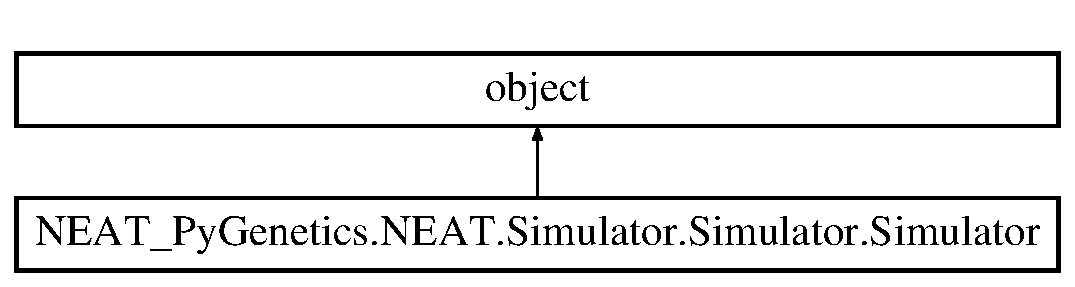
\includegraphics[height=2.000000cm]{classNEAT__PyGenetics_1_1NEAT_1_1Simulator_1_1Simulator_1_1Simulator}
\end{center}
\end{figure}
\subsection*{Public Member Functions}
\begin{DoxyCompactItemize}
\item 
def \hyperlink{classNEAT__PyGenetics_1_1NEAT_1_1Simulator_1_1Simulator_1_1Simulator_ab768445b7d9b16282919f062e0a42761}{\+\_\+\+\_\+init\+\_\+\+\_\+}
\item 
def \hyperlink{classNEAT__PyGenetics_1_1NEAT_1_1Simulator_1_1Simulator_1_1Simulator_a0e362a7174cae20d0a23b69109ac15bc}{simulate\+\_\+genome}
\end{DoxyCompactItemize}
\subsection*{Static Public Attributes}
\begin{DoxyCompactItemize}
\item 
\hyperlink{classNEAT__PyGenetics_1_1NEAT_1_1Simulator_1_1Simulator_1_1Simulator_abbacbfee6def9b5025447526cfb6152d}{simulation\+\_\+genome}
\item 
\hyperlink{classNEAT__PyGenetics_1_1NEAT_1_1Simulator_1_1Simulator_1_1Simulator_a6ebf16f89e5a3f48064b85f3acd0c9e9}{inputs}
\end{DoxyCompactItemize}


\subsection{Constructor \& Destructor Documentation}
\index{N\+E\+A\+T\+\_\+\+Py\+Genetics\+::\+N\+E\+A\+T\+::\+Simulator\+::\+Simulator\+::\+Simulator@{N\+E\+A\+T\+\_\+\+Py\+Genetics\+::\+N\+E\+A\+T\+::\+Simulator\+::\+Simulator\+::\+Simulator}!\+\_\+\+\_\+init\+\_\+\+\_\+@{\+\_\+\+\_\+init\+\_\+\+\_\+}}
\index{\+\_\+\+\_\+init\+\_\+\+\_\+@{\+\_\+\+\_\+init\+\_\+\+\_\+}!N\+E\+A\+T\+\_\+\+Py\+Genetics\+::\+N\+E\+A\+T\+::\+Simulator\+::\+Simulator\+::\+Simulator@{N\+E\+A\+T\+\_\+\+Py\+Genetics\+::\+N\+E\+A\+T\+::\+Simulator\+::\+Simulator\+::\+Simulator}}
\subsubsection[{\texorpdfstring{\+\_\+\+\_\+init\+\_\+\+\_\+}{__init__}}]{\setlength{\rightskip}{0pt plus 5cm}def N\+E\+A\+T\+\_\+\+Py\+Genetics.\+N\+E\+A\+T.\+Simulator.\+Simulator.\+Simulator.\+\_\+\+\_\+init\+\_\+\+\_\+ (
\begin{DoxyParamCaption}
\item[{}]{self, }
\item[{}]{gene\+\_\+repository}
\end{DoxyParamCaption}
)}\hypertarget{classNEAT__PyGenetics_1_1NEAT_1_1Simulator_1_1Simulator_1_1Simulator_ab768445b7d9b16282919f062e0a42761}{}\label{classNEAT__PyGenetics_1_1NEAT_1_1Simulator_1_1Simulator_1_1Simulator_ab768445b7d9b16282919f062e0a42761}


\subsection{Member Function Documentation}
\index{N\+E\+A\+T\+\_\+\+Py\+Genetics\+::\+N\+E\+A\+T\+::\+Simulator\+::\+Simulator\+::\+Simulator@{N\+E\+A\+T\+\_\+\+Py\+Genetics\+::\+N\+E\+A\+T\+::\+Simulator\+::\+Simulator\+::\+Simulator}!simulate\+\_\+genome@{simulate\+\_\+genome}}
\index{simulate\+\_\+genome@{simulate\+\_\+genome}!N\+E\+A\+T\+\_\+\+Py\+Genetics\+::\+N\+E\+A\+T\+::\+Simulator\+::\+Simulator\+::\+Simulator@{N\+E\+A\+T\+\_\+\+Py\+Genetics\+::\+N\+E\+A\+T\+::\+Simulator\+::\+Simulator\+::\+Simulator}}
\subsubsection[{\texorpdfstring{simulate\+\_\+genome}{simulate_genome}}]{\setlength{\rightskip}{0pt plus 5cm}def N\+E\+A\+T\+\_\+\+Py\+Genetics.\+N\+E\+A\+T.\+Simulator.\+Simulator.\+Simulator.\+simulate\+\_\+genome (
\begin{DoxyParamCaption}
\item[{}]{self, }
\item[{}]{storage\+\_\+genome}
\end{DoxyParamCaption}
)}\hypertarget{classNEAT__PyGenetics_1_1NEAT_1_1Simulator_1_1Simulator_1_1Simulator_a0e362a7174cae20d0a23b69109ac15bc}{}\label{classNEAT__PyGenetics_1_1NEAT_1_1Simulator_1_1Simulator_1_1Simulator_a0e362a7174cae20d0a23b69109ac15bc}


\subsection{Member Data Documentation}
\index{N\+E\+A\+T\+\_\+\+Py\+Genetics\+::\+N\+E\+A\+T\+::\+Simulator\+::\+Simulator\+::\+Simulator@{N\+E\+A\+T\+\_\+\+Py\+Genetics\+::\+N\+E\+A\+T\+::\+Simulator\+::\+Simulator\+::\+Simulator}!inputs@{inputs}}
\index{inputs@{inputs}!N\+E\+A\+T\+\_\+\+Py\+Genetics\+::\+N\+E\+A\+T\+::\+Simulator\+::\+Simulator\+::\+Simulator@{N\+E\+A\+T\+\_\+\+Py\+Genetics\+::\+N\+E\+A\+T\+::\+Simulator\+::\+Simulator\+::\+Simulator}}
\subsubsection[{\texorpdfstring{inputs}{inputs}}]{\setlength{\rightskip}{0pt plus 5cm}N\+E\+A\+T\+\_\+\+Py\+Genetics.\+N\+E\+A\+T.\+Simulator.\+Simulator.\+Simulator.\+inputs\hspace{0.3cm}{\ttfamily [static]}}\hypertarget{classNEAT__PyGenetics_1_1NEAT_1_1Simulator_1_1Simulator_1_1Simulator_a6ebf16f89e5a3f48064b85f3acd0c9e9}{}\label{classNEAT__PyGenetics_1_1NEAT_1_1Simulator_1_1Simulator_1_1Simulator_a6ebf16f89e5a3f48064b85f3acd0c9e9}
\index{N\+E\+A\+T\+\_\+\+Py\+Genetics\+::\+N\+E\+A\+T\+::\+Simulator\+::\+Simulator\+::\+Simulator@{N\+E\+A\+T\+\_\+\+Py\+Genetics\+::\+N\+E\+A\+T\+::\+Simulator\+::\+Simulator\+::\+Simulator}!simulation\+\_\+genome@{simulation\+\_\+genome}}
\index{simulation\+\_\+genome@{simulation\+\_\+genome}!N\+E\+A\+T\+\_\+\+Py\+Genetics\+::\+N\+E\+A\+T\+::\+Simulator\+::\+Simulator\+::\+Simulator@{N\+E\+A\+T\+\_\+\+Py\+Genetics\+::\+N\+E\+A\+T\+::\+Simulator\+::\+Simulator\+::\+Simulator}}
\subsubsection[{\texorpdfstring{simulation\+\_\+genome}{simulation_genome}}]{\setlength{\rightskip}{0pt plus 5cm}N\+E\+A\+T\+\_\+\+Py\+Genetics.\+N\+E\+A\+T.\+Simulator.\+Simulator.\+Simulator.\+simulation\+\_\+genome\hspace{0.3cm}{\ttfamily [static]}}\hypertarget{classNEAT__PyGenetics_1_1NEAT_1_1Simulator_1_1Simulator_1_1Simulator_abbacbfee6def9b5025447526cfb6152d}{}\label{classNEAT__PyGenetics_1_1NEAT_1_1Simulator_1_1Simulator_1_1Simulator_abbacbfee6def9b5025447526cfb6152d}


The documentation for this class was generated from the following file\+:\begin{DoxyCompactItemize}
\item 
N\+E\+A\+T/\+Simulator/\hyperlink{Simulator_8py}{Simulator.\+py}\end{DoxyCompactItemize}

\hypertarget{classNEAT__PyGenetics_1_1NEAT_1_1ErrorHandling_1_1Exceptions_1_1SocketAlreadyUsedException_1_1SocketAlreadyUsedException}{}\section{N\+E\+A\+T\+\_\+\+Py\+Genetics.\+N\+E\+A\+T.\+Error\+Handling.\+Exceptions.\+Socket\+Already\+Used\+Exception.\+Socket\+Already\+Used\+Exception Class Reference}
\label{classNEAT__PyGenetics_1_1NEAT_1_1ErrorHandling_1_1Exceptions_1_1SocketAlreadyUsedException_1_1SocketAlreadyUsedException}\index{N\+E\+A\+T\+\_\+\+Py\+Genetics.\+N\+E\+A\+T.\+Error\+Handling.\+Exceptions.\+Socket\+Already\+Used\+Exception.\+Socket\+Already\+Used\+Exception@{N\+E\+A\+T\+\_\+\+Py\+Genetics.\+N\+E\+A\+T.\+Error\+Handling.\+Exceptions.\+Socket\+Already\+Used\+Exception.\+Socket\+Already\+Used\+Exception}}
Inheritance diagram for N\+E\+A\+T\+\_\+\+Py\+Genetics.\+N\+E\+A\+T.\+Error\+Handling.\+Exceptions.\+Socket\+Already\+Used\+Exception.\+Socket\+Already\+Used\+Exception\+:\begin{figure}[H]
\begin{center}
\leavevmode
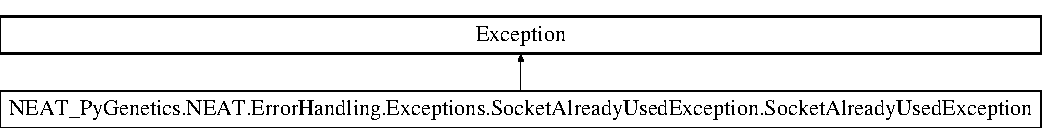
\includegraphics[height=1.723077cm]{classNEAT__PyGenetics_1_1NEAT_1_1ErrorHandling_1_1Exceptions_1_1SocketAlreadyUsedException_1_1SocketAlreadyUsedException}
\end{center}
\end{figure}
\subsection*{Public Member Functions}
\begin{DoxyCompactItemize}
\item 
def \hyperlink{classNEAT__PyGenetics_1_1NEAT_1_1ErrorHandling_1_1Exceptions_1_1SocketAlreadyUsedException_1_1SocketAlreadyUsedException_aa78052a441ad0d25947f06f3ed625c1c}{\+\_\+\+\_\+init\+\_\+\+\_\+} (self, message=\char`\"{}\char`\"{}, errors=None)
\end{DoxyCompactItemize}


\subsection{Constructor \& Destructor Documentation}
\index{N\+E\+A\+T\+\_\+\+Py\+Genetics\+::\+N\+E\+A\+T\+::\+Error\+Handling\+::\+Exceptions\+::\+Socket\+Already\+Used\+Exception\+::\+Socket\+Already\+Used\+Exception@{N\+E\+A\+T\+\_\+\+Py\+Genetics\+::\+N\+E\+A\+T\+::\+Error\+Handling\+::\+Exceptions\+::\+Socket\+Already\+Used\+Exception\+::\+Socket\+Already\+Used\+Exception}!\+\_\+\+\_\+init\+\_\+\+\_\+@{\+\_\+\+\_\+init\+\_\+\+\_\+}}
\index{\+\_\+\+\_\+init\+\_\+\+\_\+@{\+\_\+\+\_\+init\+\_\+\+\_\+}!N\+E\+A\+T\+\_\+\+Py\+Genetics\+::\+N\+E\+A\+T\+::\+Error\+Handling\+::\+Exceptions\+::\+Socket\+Already\+Used\+Exception\+::\+Socket\+Already\+Used\+Exception@{N\+E\+A\+T\+\_\+\+Py\+Genetics\+::\+N\+E\+A\+T\+::\+Error\+Handling\+::\+Exceptions\+::\+Socket\+Already\+Used\+Exception\+::\+Socket\+Already\+Used\+Exception}}
\subsubsection[{\texorpdfstring{\+\_\+\+\_\+init\+\_\+\+\_\+(self, message="""", errors=\+None)}{__init__(self, message="", errors=None)}}]{\setlength{\rightskip}{0pt plus 5cm}def N\+E\+A\+T\+\_\+\+Py\+Genetics.\+N\+E\+A\+T.\+Error\+Handling.\+Exceptions.\+Socket\+Already\+Used\+Exception.\+Socket\+Already\+Used\+Exception.\+\_\+\+\_\+init\+\_\+\+\_\+ (
\begin{DoxyParamCaption}
\item[{}]{self, }
\item[{}]{message = {\ttfamily \char`\"{}\char`\"{}}, }
\item[{}]{errors = {\ttfamily None}}
\end{DoxyParamCaption}
)}\hypertarget{classNEAT__PyGenetics_1_1NEAT_1_1ErrorHandling_1_1Exceptions_1_1SocketAlreadyUsedException_1_1SocketAlreadyUsedException_aa78052a441ad0d25947f06f3ed625c1c}{}\label{classNEAT__PyGenetics_1_1NEAT_1_1ErrorHandling_1_1Exceptions_1_1SocketAlreadyUsedException_1_1SocketAlreadyUsedException_aa78052a441ad0d25947f06f3ed625c1c}


The documentation for this class was generated from the following file\+:\begin{DoxyCompactItemize}
\item 
N\+E\+A\+T/\+Error\+Handling/\+Exceptions/\hyperlink{SocketAlreadyUsedException_8py}{Socket\+Already\+Used\+Exception.\+py}\end{DoxyCompactItemize}

\hypertarget{classNEAT__PyGenetics_1_1NEAT_1_1ErrorHandling_1_1Exceptions_1_1SocketRuntimeException_1_1SocketRuntimeException}{}\section{N\+E\+A\+T\+\_\+\+Py\+Genetics.\+N\+E\+A\+T.\+Error\+Handling.\+Exceptions.\+Socket\+Runtime\+Exception.\+Socket\+Runtime\+Exception Class Reference}
\label{classNEAT__PyGenetics_1_1NEAT_1_1ErrorHandling_1_1Exceptions_1_1SocketRuntimeException_1_1SocketRuntimeException}\index{N\+E\+A\+T\+\_\+\+Py\+Genetics.\+N\+E\+A\+T.\+Error\+Handling.\+Exceptions.\+Socket\+Runtime\+Exception.\+Socket\+Runtime\+Exception@{N\+E\+A\+T\+\_\+\+Py\+Genetics.\+N\+E\+A\+T.\+Error\+Handling.\+Exceptions.\+Socket\+Runtime\+Exception.\+Socket\+Runtime\+Exception}}
Inheritance diagram for N\+E\+A\+T\+\_\+\+Py\+Genetics.\+N\+E\+A\+T.\+Error\+Handling.\+Exceptions.\+Socket\+Runtime\+Exception.\+Socket\+Runtime\+Exception\+:\begin{figure}[H]
\begin{center}
\leavevmode
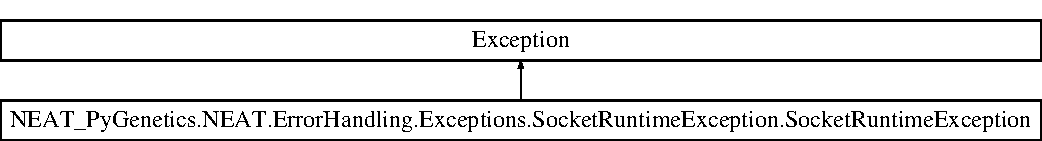
\includegraphics[height=1.891892cm]{classNEAT__PyGenetics_1_1NEAT_1_1ErrorHandling_1_1Exceptions_1_1SocketRuntimeException_1_1SocketRuntimeException}
\end{center}
\end{figure}
\subsection*{Public Member Functions}
\begin{DoxyCompactItemize}
\item 
def \hyperlink{classNEAT__PyGenetics_1_1NEAT_1_1ErrorHandling_1_1Exceptions_1_1SocketRuntimeException_1_1SocketRuntimeException_a747071f76bd0ecd08342e4ac9d7a5e33}{\+\_\+\+\_\+init\+\_\+\+\_\+} (self, message=\char`\"{}\char`\"{}, errors=None)
\end{DoxyCompactItemize}


\subsection{Constructor \& Destructor Documentation}
\index{N\+E\+A\+T\+\_\+\+Py\+Genetics\+::\+N\+E\+A\+T\+::\+Error\+Handling\+::\+Exceptions\+::\+Socket\+Runtime\+Exception\+::\+Socket\+Runtime\+Exception@{N\+E\+A\+T\+\_\+\+Py\+Genetics\+::\+N\+E\+A\+T\+::\+Error\+Handling\+::\+Exceptions\+::\+Socket\+Runtime\+Exception\+::\+Socket\+Runtime\+Exception}!\+\_\+\+\_\+init\+\_\+\+\_\+@{\+\_\+\+\_\+init\+\_\+\+\_\+}}
\index{\+\_\+\+\_\+init\+\_\+\+\_\+@{\+\_\+\+\_\+init\+\_\+\+\_\+}!N\+E\+A\+T\+\_\+\+Py\+Genetics\+::\+N\+E\+A\+T\+::\+Error\+Handling\+::\+Exceptions\+::\+Socket\+Runtime\+Exception\+::\+Socket\+Runtime\+Exception@{N\+E\+A\+T\+\_\+\+Py\+Genetics\+::\+N\+E\+A\+T\+::\+Error\+Handling\+::\+Exceptions\+::\+Socket\+Runtime\+Exception\+::\+Socket\+Runtime\+Exception}}
\subsubsection[{\texorpdfstring{\+\_\+\+\_\+init\+\_\+\+\_\+(self, message="""", errors=\+None)}{__init__(self, message="", errors=None)}}]{\setlength{\rightskip}{0pt plus 5cm}def N\+E\+A\+T\+\_\+\+Py\+Genetics.\+N\+E\+A\+T.\+Error\+Handling.\+Exceptions.\+Socket\+Runtime\+Exception.\+Socket\+Runtime\+Exception.\+\_\+\+\_\+init\+\_\+\+\_\+ (
\begin{DoxyParamCaption}
\item[{}]{self, }
\item[{}]{message = {\ttfamily \char`\"{}\char`\"{}}, }
\item[{}]{errors = {\ttfamily None}}
\end{DoxyParamCaption}
)}\hypertarget{classNEAT__PyGenetics_1_1NEAT_1_1ErrorHandling_1_1Exceptions_1_1SocketRuntimeException_1_1SocketRuntimeException_a747071f76bd0ecd08342e4ac9d7a5e33}{}\label{classNEAT__PyGenetics_1_1NEAT_1_1ErrorHandling_1_1Exceptions_1_1SocketRuntimeException_1_1SocketRuntimeException_a747071f76bd0ecd08342e4ac9d7a5e33}


The documentation for this class was generated from the following file\+:\begin{DoxyCompactItemize}
\item 
N\+E\+A\+T/\+Error\+Handling/\+Exceptions/\hyperlink{SocketRuntimeException_8py}{Socket\+Runtime\+Exception.\+py}\end{DoxyCompactItemize}

\hypertarget{classNEAT__PyGenetics_1_1NEAT_1_1ErrorHandling_1_1StartupCheck_1_1StartupCheck}{}\section{N\+E\+A\+T\+\_\+\+Py\+Genetics.\+N\+E\+A\+T.\+Error\+Handling.\+Startup\+Check.\+Startup\+Check Class Reference}
\label{classNEAT__PyGenetics_1_1NEAT_1_1ErrorHandling_1_1StartupCheck_1_1StartupCheck}\index{N\+E\+A\+T\+\_\+\+Py\+Genetics.\+N\+E\+A\+T.\+Error\+Handling.\+Startup\+Check.\+Startup\+Check@{N\+E\+A\+T\+\_\+\+Py\+Genetics.\+N\+E\+A\+T.\+Error\+Handling.\+Startup\+Check.\+Startup\+Check}}
Inheritance diagram for N\+E\+A\+T\+\_\+\+Py\+Genetics.\+N\+E\+A\+T.\+Error\+Handling.\+Startup\+Check.\+Startup\+Check\+:\begin{figure}[H]
\begin{center}
\leavevmode
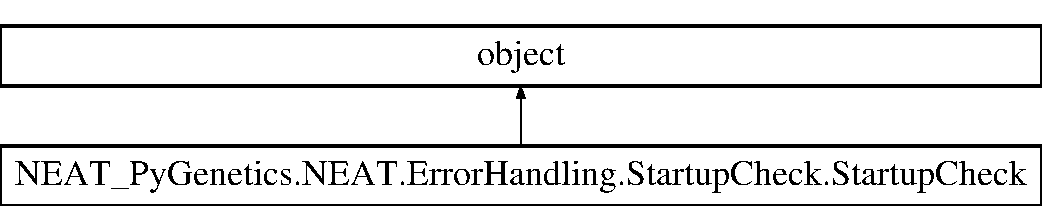
\includegraphics[height=2.000000cm]{classNEAT__PyGenetics_1_1NEAT_1_1ErrorHandling_1_1StartupCheck_1_1StartupCheck}
\end{center}
\end{figure}
\subsection*{Public Member Functions}
\begin{DoxyCompactItemize}
\item 
def \hyperlink{classNEAT__PyGenetics_1_1NEAT_1_1ErrorHandling_1_1StartupCheck_1_1StartupCheck_a1e599ee38990fc5249559baf65685459}{\+\_\+\+\_\+init\+\_\+\+\_\+} (self)
\item 
def \hyperlink{classNEAT__PyGenetics_1_1NEAT_1_1ErrorHandling_1_1StartupCheck_1_1StartupCheck_a03356f117dc673d35d69882ecabad2a3}{run} (self)
\end{DoxyCompactItemize}
\subsection*{Public Attributes}
\begin{DoxyCompactItemize}
\item 
\hyperlink{classNEAT__PyGenetics_1_1NEAT_1_1ErrorHandling_1_1StartupCheck_1_1StartupCheck_afca8d845c7a7796c0963e0d49ec96786}{con}
\item 
\hyperlink{classNEAT__PyGenetics_1_1NEAT_1_1ErrorHandling_1_1StartupCheck_1_1StartupCheck_a9defc0bb9535a560af330658f89337ac}{rep}
\end{DoxyCompactItemize}


\subsection{Constructor \& Destructor Documentation}
\index{N\+E\+A\+T\+\_\+\+Py\+Genetics\+::\+N\+E\+A\+T\+::\+Error\+Handling\+::\+Startup\+Check\+::\+Startup\+Check@{N\+E\+A\+T\+\_\+\+Py\+Genetics\+::\+N\+E\+A\+T\+::\+Error\+Handling\+::\+Startup\+Check\+::\+Startup\+Check}!\+\_\+\+\_\+init\+\_\+\+\_\+@{\+\_\+\+\_\+init\+\_\+\+\_\+}}
\index{\+\_\+\+\_\+init\+\_\+\+\_\+@{\+\_\+\+\_\+init\+\_\+\+\_\+}!N\+E\+A\+T\+\_\+\+Py\+Genetics\+::\+N\+E\+A\+T\+::\+Error\+Handling\+::\+Startup\+Check\+::\+Startup\+Check@{N\+E\+A\+T\+\_\+\+Py\+Genetics\+::\+N\+E\+A\+T\+::\+Error\+Handling\+::\+Startup\+Check\+::\+Startup\+Check}}
\subsubsection[{\texorpdfstring{\+\_\+\+\_\+init\+\_\+\+\_\+(self)}{__init__(self)}}]{\setlength{\rightskip}{0pt plus 5cm}def N\+E\+A\+T\+\_\+\+Py\+Genetics.\+N\+E\+A\+T.\+Error\+Handling.\+Startup\+Check.\+Startup\+Check.\+\_\+\+\_\+init\+\_\+\+\_\+ (
\begin{DoxyParamCaption}
\item[{}]{self}
\end{DoxyParamCaption}
)}\hypertarget{classNEAT__PyGenetics_1_1NEAT_1_1ErrorHandling_1_1StartupCheck_1_1StartupCheck_a1e599ee38990fc5249559baf65685459}{}\label{classNEAT__PyGenetics_1_1NEAT_1_1ErrorHandling_1_1StartupCheck_1_1StartupCheck_a1e599ee38990fc5249559baf65685459}


\subsection{Member Function Documentation}
\index{N\+E\+A\+T\+\_\+\+Py\+Genetics\+::\+N\+E\+A\+T\+::\+Error\+Handling\+::\+Startup\+Check\+::\+Startup\+Check@{N\+E\+A\+T\+\_\+\+Py\+Genetics\+::\+N\+E\+A\+T\+::\+Error\+Handling\+::\+Startup\+Check\+::\+Startup\+Check}!run@{run}}
\index{run@{run}!N\+E\+A\+T\+\_\+\+Py\+Genetics\+::\+N\+E\+A\+T\+::\+Error\+Handling\+::\+Startup\+Check\+::\+Startup\+Check@{N\+E\+A\+T\+\_\+\+Py\+Genetics\+::\+N\+E\+A\+T\+::\+Error\+Handling\+::\+Startup\+Check\+::\+Startup\+Check}}
\subsubsection[{\texorpdfstring{run(self)}{run(self)}}]{\setlength{\rightskip}{0pt plus 5cm}def N\+E\+A\+T\+\_\+\+Py\+Genetics.\+N\+E\+A\+T.\+Error\+Handling.\+Startup\+Check.\+Startup\+Check.\+run (
\begin{DoxyParamCaption}
\item[{}]{self}
\end{DoxyParamCaption}
)}\hypertarget{classNEAT__PyGenetics_1_1NEAT_1_1ErrorHandling_1_1StartupCheck_1_1StartupCheck_a03356f117dc673d35d69882ecabad2a3}{}\label{classNEAT__PyGenetics_1_1NEAT_1_1ErrorHandling_1_1StartupCheck_1_1StartupCheck_a03356f117dc673d35d69882ecabad2a3}


\subsection{Member Data Documentation}
\index{N\+E\+A\+T\+\_\+\+Py\+Genetics\+::\+N\+E\+A\+T\+::\+Error\+Handling\+::\+Startup\+Check\+::\+Startup\+Check@{N\+E\+A\+T\+\_\+\+Py\+Genetics\+::\+N\+E\+A\+T\+::\+Error\+Handling\+::\+Startup\+Check\+::\+Startup\+Check}!con@{con}}
\index{con@{con}!N\+E\+A\+T\+\_\+\+Py\+Genetics\+::\+N\+E\+A\+T\+::\+Error\+Handling\+::\+Startup\+Check\+::\+Startup\+Check@{N\+E\+A\+T\+\_\+\+Py\+Genetics\+::\+N\+E\+A\+T\+::\+Error\+Handling\+::\+Startup\+Check\+::\+Startup\+Check}}
\subsubsection[{\texorpdfstring{con}{con}}]{\setlength{\rightskip}{0pt plus 5cm}N\+E\+A\+T\+\_\+\+Py\+Genetics.\+N\+E\+A\+T.\+Error\+Handling.\+Startup\+Check.\+Startup\+Check.\+con}\hypertarget{classNEAT__PyGenetics_1_1NEAT_1_1ErrorHandling_1_1StartupCheck_1_1StartupCheck_afca8d845c7a7796c0963e0d49ec96786}{}\label{classNEAT__PyGenetics_1_1NEAT_1_1ErrorHandling_1_1StartupCheck_1_1StartupCheck_afca8d845c7a7796c0963e0d49ec96786}
\index{N\+E\+A\+T\+\_\+\+Py\+Genetics\+::\+N\+E\+A\+T\+::\+Error\+Handling\+::\+Startup\+Check\+::\+Startup\+Check@{N\+E\+A\+T\+\_\+\+Py\+Genetics\+::\+N\+E\+A\+T\+::\+Error\+Handling\+::\+Startup\+Check\+::\+Startup\+Check}!rep@{rep}}
\index{rep@{rep}!N\+E\+A\+T\+\_\+\+Py\+Genetics\+::\+N\+E\+A\+T\+::\+Error\+Handling\+::\+Startup\+Check\+::\+Startup\+Check@{N\+E\+A\+T\+\_\+\+Py\+Genetics\+::\+N\+E\+A\+T\+::\+Error\+Handling\+::\+Startup\+Check\+::\+Startup\+Check}}
\subsubsection[{\texorpdfstring{rep}{rep}}]{\setlength{\rightskip}{0pt plus 5cm}N\+E\+A\+T\+\_\+\+Py\+Genetics.\+N\+E\+A\+T.\+Error\+Handling.\+Startup\+Check.\+Startup\+Check.\+rep}\hypertarget{classNEAT__PyGenetics_1_1NEAT_1_1ErrorHandling_1_1StartupCheck_1_1StartupCheck_a9defc0bb9535a560af330658f89337ac}{}\label{classNEAT__PyGenetics_1_1NEAT_1_1ErrorHandling_1_1StartupCheck_1_1StartupCheck_a9defc0bb9535a560af330658f89337ac}


The documentation for this class was generated from the following file\+:\begin{DoxyCompactItemize}
\item 
N\+E\+A\+T/\+Error\+Handling/\hyperlink{StartupCheck_8py}{Startup\+Check.\+py}\end{DoxyCompactItemize}

\hypertarget{classNEAT__PyGenetics_1_1NEAT_1_1ErrorHandling_1_1Exceptions_1_1StartupCheckException_1_1StartupCheckException}{}\section{N\+E\+A\+T\+\_\+\+Py\+Genetics.\+N\+E\+A\+T.\+Error\+Handling.\+Exceptions.\+Startup\+Check\+Exception.\+Startup\+Check\+Exception Class Reference}
\label{classNEAT__PyGenetics_1_1NEAT_1_1ErrorHandling_1_1Exceptions_1_1StartupCheckException_1_1StartupCheckException}\index{N\+E\+A\+T\+\_\+\+Py\+Genetics.\+N\+E\+A\+T.\+Error\+Handling.\+Exceptions.\+Startup\+Check\+Exception.\+Startup\+Check\+Exception@{N\+E\+A\+T\+\_\+\+Py\+Genetics.\+N\+E\+A\+T.\+Error\+Handling.\+Exceptions.\+Startup\+Check\+Exception.\+Startup\+Check\+Exception}}
Inheritance diagram for N\+E\+A\+T\+\_\+\+Py\+Genetics.\+N\+E\+A\+T.\+Error\+Handling.\+Exceptions.\+Startup\+Check\+Exception.\+Startup\+Check\+Exception\+:\begin{figure}[H]
\begin{center}
\leavevmode
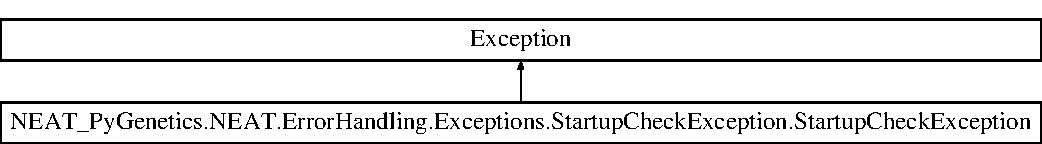
\includegraphics[height=1.931034cm]{classNEAT__PyGenetics_1_1NEAT_1_1ErrorHandling_1_1Exceptions_1_1StartupCheckException_1_1StartupCheckException}
\end{center}
\end{figure}
\subsection*{Public Member Functions}
\begin{DoxyCompactItemize}
\item 
def \hyperlink{classNEAT__PyGenetics_1_1NEAT_1_1ErrorHandling_1_1Exceptions_1_1StartupCheckException_1_1StartupCheckException_a39cbd39c3a77f3acc9c3feb3bfb84d7e}{\+\_\+\+\_\+init\+\_\+\+\_\+} (self, message=\char`\"{}\char`\"{}, errors=None)
\end{DoxyCompactItemize}


\subsection{Constructor \& Destructor Documentation}
\index{N\+E\+A\+T\+\_\+\+Py\+Genetics\+::\+N\+E\+A\+T\+::\+Error\+Handling\+::\+Exceptions\+::\+Startup\+Check\+Exception\+::\+Startup\+Check\+Exception@{N\+E\+A\+T\+\_\+\+Py\+Genetics\+::\+N\+E\+A\+T\+::\+Error\+Handling\+::\+Exceptions\+::\+Startup\+Check\+Exception\+::\+Startup\+Check\+Exception}!\+\_\+\+\_\+init\+\_\+\+\_\+@{\+\_\+\+\_\+init\+\_\+\+\_\+}}
\index{\+\_\+\+\_\+init\+\_\+\+\_\+@{\+\_\+\+\_\+init\+\_\+\+\_\+}!N\+E\+A\+T\+\_\+\+Py\+Genetics\+::\+N\+E\+A\+T\+::\+Error\+Handling\+::\+Exceptions\+::\+Startup\+Check\+Exception\+::\+Startup\+Check\+Exception@{N\+E\+A\+T\+\_\+\+Py\+Genetics\+::\+N\+E\+A\+T\+::\+Error\+Handling\+::\+Exceptions\+::\+Startup\+Check\+Exception\+::\+Startup\+Check\+Exception}}
\subsubsection[{\texorpdfstring{\+\_\+\+\_\+init\+\_\+\+\_\+(self, message="""", errors=\+None)}{__init__(self, message="", errors=None)}}]{\setlength{\rightskip}{0pt plus 5cm}def N\+E\+A\+T\+\_\+\+Py\+Genetics.\+N\+E\+A\+T.\+Error\+Handling.\+Exceptions.\+Startup\+Check\+Exception.\+Startup\+Check\+Exception.\+\_\+\+\_\+init\+\_\+\+\_\+ (
\begin{DoxyParamCaption}
\item[{}]{self, }
\item[{}]{message = {\ttfamily \char`\"{}\char`\"{}}, }
\item[{}]{errors = {\ttfamily None}}
\end{DoxyParamCaption}
)}\hypertarget{classNEAT__PyGenetics_1_1NEAT_1_1ErrorHandling_1_1Exceptions_1_1StartupCheckException_1_1StartupCheckException_a39cbd39c3a77f3acc9c3feb3bfb84d7e}{}\label{classNEAT__PyGenetics_1_1NEAT_1_1ErrorHandling_1_1Exceptions_1_1StartupCheckException_1_1StartupCheckException_a39cbd39c3a77f3acc9c3feb3bfb84d7e}


The documentation for this class was generated from the following file\+:\begin{DoxyCompactItemize}
\item 
N\+E\+A\+T/\+Error\+Handling/\+Exceptions/\hyperlink{StartupCheckException_8py}{Startup\+Check\+Exception.\+py}\end{DoxyCompactItemize}

\hypertarget{classNEAT__PyGenetics_1_1NEAT_1_1GenomeStructures_1_1StorageStructure_1_1StorageGenome_1_1StorageGenome}{}\section{N\+E\+A\+T\+\_\+\+Py\+Genetics.\+N\+E\+A\+T.\+Genome\+Structures.\+Storage\+Structure.\+Storage\+Genome.\+Storage\+Genome Class Reference}
\label{classNEAT__PyGenetics_1_1NEAT_1_1GenomeStructures_1_1StorageStructure_1_1StorageGenome_1_1StorageGenome}\index{N\+E\+A\+T\+\_\+\+Py\+Genetics.\+N\+E\+A\+T.\+Genome\+Structures.\+Storage\+Structure.\+Storage\+Genome.\+Storage\+Genome@{N\+E\+A\+T\+\_\+\+Py\+Genetics.\+N\+E\+A\+T.\+Genome\+Structures.\+Storage\+Structure.\+Storage\+Genome.\+Storage\+Genome}}


A data structure for storing genome information in a compact way.  


Inheritance diagram for N\+E\+A\+T\+\_\+\+Py\+Genetics.\+N\+E\+A\+T.\+Genome\+Structures.\+Storage\+Structure.\+Storage\+Genome.\+Storage\+Genome\+:\begin{figure}[H]
\begin{center}
\leavevmode
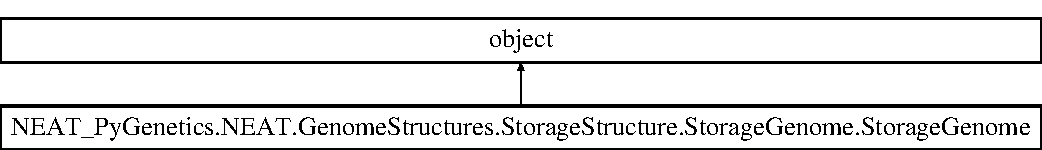
\includegraphics[height=2.000000cm]{classNEAT__PyGenetics_1_1NEAT_1_1GenomeStructures_1_1StorageStructure_1_1StorageGenome_1_1StorageGenome}
\end{center}
\end{figure}
\subsection*{Public Member Functions}
\begin{DoxyCompactItemize}
\item 
def \hyperlink{classNEAT__PyGenetics_1_1NEAT_1_1GenomeStructures_1_1StorageStructure_1_1StorageGenome_1_1StorageGenome_a8b7615cf97ad4ce4c3805ecde57637c8}{\+\_\+\+\_\+init\+\_\+\+\_\+}
\begin{DoxyCompactList}\small\item\em \+:param genome\+: If genome is given, its inputs are copied (except for id) \+:param inputs\+: A list of strings, representing the inputs nodes\textquotesingle{} labels \end{DoxyCompactList}\item 
def \hyperlink{classNEAT__PyGenetics_1_1NEAT_1_1GenomeStructures_1_1StorageStructure_1_1StorageGenome_1_1StorageGenome_a0d0ae3acf7162d05cb40fe5eaff9ada9}{\+\_\+\+\_\+eq\+\_\+\+\_\+}
\item 
def \hyperlink{classNEAT__PyGenetics_1_1NEAT_1_1GenomeStructures_1_1StorageStructure_1_1StorageGenome_1_1StorageGenome_a536876e28c6ee27477de23a369e11daa}{genome\+\_\+id} (self)
\end{DoxyCompactItemize}
\subsection*{Static Public Attributes}
\begin{DoxyCompactItemize}
\item 
\hyperlink{classNEAT__PyGenetics_1_1NEAT_1_1GenomeStructures_1_1StorageStructure_1_1StorageGenome_1_1StorageGenome_ae1e47996623ce538b3450f2415d57bc3}{is\+\_\+alive}
\item 
\hyperlink{classNEAT__PyGenetics_1_1NEAT_1_1GenomeStructures_1_1StorageStructure_1_1StorageGenome_1_1StorageGenome_a919c35fa0dfc5d4a81b008bef83c3ac9}{fitness}
\item 
\hyperlink{classNEAT__PyGenetics_1_1NEAT_1_1GenomeStructures_1_1StorageStructure_1_1StorageGenome_1_1StorageGenome_ad0bd7b5a391f6df7f56f60294fee0a00}{inputs}
\item 
\hyperlink{classNEAT__PyGenetics_1_1NEAT_1_1GenomeStructures_1_1StorageStructure_1_1StorageGenome_1_1StorageGenome_a69f429018a927d4919d4468054cf49ea}{outputs}
\item 
\hyperlink{classNEAT__PyGenetics_1_1NEAT_1_1GenomeStructures_1_1StorageStructure_1_1StorageGenome_1_1StorageGenome_a82003c70917d4c96053c6cea930383ce}{genes}
\item 
\hyperlink{classNEAT__PyGenetics_1_1NEAT_1_1GenomeStructures_1_1StorageStructure_1_1StorageGenome_1_1StorageGenome_a4ed1621581430cdf5791c33d1c2f6ac2}{analysis\+\_\+result}
\item 
\hyperlink{classNEAT__PyGenetics_1_1NEAT_1_1GenomeStructures_1_1StorageStructure_1_1StorageGenome_1_1StorageGenome_a4d31fdd32df12f7c1d9c6848b4ae1bcc}{cluster}
\end{DoxyCompactItemize}


\subsection{Detailed Description}
A data structure for storing genome information in a compact way. 

Attributes\+: genome\+\_\+id (\+\_\+id)\+: The Genome\textquotesingle{}s ID, unique in the population. inputs\+: A list of the ids of the input nodes. There has to be at least one gene per input that is connected to it. Represented as a list of tuples of the form (Input\+\_\+\+Label, Node-\/\+ID). outputs\+: A list of the ids of the output nodes. There has to be at least one gene per output that is connected to it. Represented as a list of tuples of the form (Output\+\_\+\+Label, Node-\/\+ID). genes\+: A list of all genes, that make up the genome. Presented as a tu-\/ ple of Gene-\/\+ID, a boolean that is true, if the gene is disabled and a Fraction that stores the weight of the gene. analysis\+\_\+result\+: A result object that is generated when analyzing the genome. This is empty per default. cluster\+: The cluster to which the Genome belongs. 

\subsection{Constructor \& Destructor Documentation}
\index{N\+E\+A\+T\+\_\+\+Py\+Genetics\+::\+N\+E\+A\+T\+::\+Genome\+Structures\+::\+Storage\+Structure\+::\+Storage\+Genome\+::\+Storage\+Genome@{N\+E\+A\+T\+\_\+\+Py\+Genetics\+::\+N\+E\+A\+T\+::\+Genome\+Structures\+::\+Storage\+Structure\+::\+Storage\+Genome\+::\+Storage\+Genome}!\+\_\+\+\_\+init\+\_\+\+\_\+@{\+\_\+\+\_\+init\+\_\+\+\_\+}}
\index{\+\_\+\+\_\+init\+\_\+\+\_\+@{\+\_\+\+\_\+init\+\_\+\+\_\+}!N\+E\+A\+T\+\_\+\+Py\+Genetics\+::\+N\+E\+A\+T\+::\+Genome\+Structures\+::\+Storage\+Structure\+::\+Storage\+Genome\+::\+Storage\+Genome@{N\+E\+A\+T\+\_\+\+Py\+Genetics\+::\+N\+E\+A\+T\+::\+Genome\+Structures\+::\+Storage\+Structure\+::\+Storage\+Genome\+::\+Storage\+Genome}}
\subsubsection[{\texorpdfstring{\+\_\+\+\_\+init\+\_\+\+\_\+}{__init__}}]{\setlength{\rightskip}{0pt plus 5cm}def N\+E\+A\+T\+\_\+\+Py\+Genetics.\+N\+E\+A\+T.\+Genome\+Structures.\+Storage\+Structure.\+Storage\+Genome.\+Storage\+Genome.\+\_\+\+\_\+init\+\_\+\+\_\+ (
\begin{DoxyParamCaption}
\item[{}]{self, }
\item[{}]{genome}
\end{DoxyParamCaption}
)}\hypertarget{classNEAT__PyGenetics_1_1NEAT_1_1GenomeStructures_1_1StorageStructure_1_1StorageGenome_1_1StorageGenome_a8b7615cf97ad4ce4c3805ecde57637c8}{}\label{classNEAT__PyGenetics_1_1NEAT_1_1GenomeStructures_1_1StorageStructure_1_1StorageGenome_1_1StorageGenome_a8b7615cf97ad4ce4c3805ecde57637c8}


\+:param genome\+: If genome is given, its inputs are copied (except for id) \+:param inputs\+: A list of strings, representing the inputs nodes\textquotesingle{} labels 



\subsection{Member Function Documentation}
\index{N\+E\+A\+T\+\_\+\+Py\+Genetics\+::\+N\+E\+A\+T\+::\+Genome\+Structures\+::\+Storage\+Structure\+::\+Storage\+Genome\+::\+Storage\+Genome@{N\+E\+A\+T\+\_\+\+Py\+Genetics\+::\+N\+E\+A\+T\+::\+Genome\+Structures\+::\+Storage\+Structure\+::\+Storage\+Genome\+::\+Storage\+Genome}!\+\_\+\+\_\+eq\+\_\+\+\_\+@{\+\_\+\+\_\+eq\+\_\+\+\_\+}}
\index{\+\_\+\+\_\+eq\+\_\+\+\_\+@{\+\_\+\+\_\+eq\+\_\+\+\_\+}!N\+E\+A\+T\+\_\+\+Py\+Genetics\+::\+N\+E\+A\+T\+::\+Genome\+Structures\+::\+Storage\+Structure\+::\+Storage\+Genome\+::\+Storage\+Genome@{N\+E\+A\+T\+\_\+\+Py\+Genetics\+::\+N\+E\+A\+T\+::\+Genome\+Structures\+::\+Storage\+Structure\+::\+Storage\+Genome\+::\+Storage\+Genome}}
\subsubsection[{\texorpdfstring{\+\_\+\+\_\+eq\+\_\+\+\_\+}{__eq__}}]{\setlength{\rightskip}{0pt plus 5cm}def N\+E\+A\+T\+\_\+\+Py\+Genetics.\+N\+E\+A\+T.\+Genome\+Structures.\+Storage\+Structure.\+Storage\+Genome.\+Storage\+Genome.\+\_\+\+\_\+eq\+\_\+\+\_\+ (
\begin{DoxyParamCaption}
\item[{}]{self, }
\item[{}]{obj}
\end{DoxyParamCaption}
)}\hypertarget{classNEAT__PyGenetics_1_1NEAT_1_1GenomeStructures_1_1StorageStructure_1_1StorageGenome_1_1StorageGenome_a0d0ae3acf7162d05cb40fe5eaff9ada9}{}\label{classNEAT__PyGenetics_1_1NEAT_1_1GenomeStructures_1_1StorageStructure_1_1StorageGenome_1_1StorageGenome_a0d0ae3acf7162d05cb40fe5eaff9ada9}
\index{N\+E\+A\+T\+\_\+\+Py\+Genetics\+::\+N\+E\+A\+T\+::\+Genome\+Structures\+::\+Storage\+Structure\+::\+Storage\+Genome\+::\+Storage\+Genome@{N\+E\+A\+T\+\_\+\+Py\+Genetics\+::\+N\+E\+A\+T\+::\+Genome\+Structures\+::\+Storage\+Structure\+::\+Storage\+Genome\+::\+Storage\+Genome}!genome\+\_\+id@{genome\+\_\+id}}
\index{genome\+\_\+id@{genome\+\_\+id}!N\+E\+A\+T\+\_\+\+Py\+Genetics\+::\+N\+E\+A\+T\+::\+Genome\+Structures\+::\+Storage\+Structure\+::\+Storage\+Genome\+::\+Storage\+Genome@{N\+E\+A\+T\+\_\+\+Py\+Genetics\+::\+N\+E\+A\+T\+::\+Genome\+Structures\+::\+Storage\+Structure\+::\+Storage\+Genome\+::\+Storage\+Genome}}
\subsubsection[{\texorpdfstring{genome\+\_\+id(self)}{genome_id(self)}}]{\setlength{\rightskip}{0pt plus 5cm}def N\+E\+A\+T\+\_\+\+Py\+Genetics.\+N\+E\+A\+T.\+Genome\+Structures.\+Storage\+Structure.\+Storage\+Genome.\+Storage\+Genome.\+genome\+\_\+id (
\begin{DoxyParamCaption}
\item[{}]{self}
\end{DoxyParamCaption}
)}\hypertarget{classNEAT__PyGenetics_1_1NEAT_1_1GenomeStructures_1_1StorageStructure_1_1StorageGenome_1_1StorageGenome_a536876e28c6ee27477de23a369e11daa}{}\label{classNEAT__PyGenetics_1_1NEAT_1_1GenomeStructures_1_1StorageStructure_1_1StorageGenome_1_1StorageGenome_a536876e28c6ee27477de23a369e11daa}


\subsection{Member Data Documentation}
\index{N\+E\+A\+T\+\_\+\+Py\+Genetics\+::\+N\+E\+A\+T\+::\+Genome\+Structures\+::\+Storage\+Structure\+::\+Storage\+Genome\+::\+Storage\+Genome@{N\+E\+A\+T\+\_\+\+Py\+Genetics\+::\+N\+E\+A\+T\+::\+Genome\+Structures\+::\+Storage\+Structure\+::\+Storage\+Genome\+::\+Storage\+Genome}!analysis\+\_\+result@{analysis\+\_\+result}}
\index{analysis\+\_\+result@{analysis\+\_\+result}!N\+E\+A\+T\+\_\+\+Py\+Genetics\+::\+N\+E\+A\+T\+::\+Genome\+Structures\+::\+Storage\+Structure\+::\+Storage\+Genome\+::\+Storage\+Genome@{N\+E\+A\+T\+\_\+\+Py\+Genetics\+::\+N\+E\+A\+T\+::\+Genome\+Structures\+::\+Storage\+Structure\+::\+Storage\+Genome\+::\+Storage\+Genome}}
\subsubsection[{\texorpdfstring{analysis\+\_\+result}{analysis_result}}]{\setlength{\rightskip}{0pt plus 5cm}N\+E\+A\+T\+\_\+\+Py\+Genetics.\+N\+E\+A\+T.\+Genome\+Structures.\+Storage\+Structure.\+Storage\+Genome.\+Storage\+Genome.\+analysis\+\_\+result\hspace{0.3cm}{\ttfamily [static]}}\hypertarget{classNEAT__PyGenetics_1_1NEAT_1_1GenomeStructures_1_1StorageStructure_1_1StorageGenome_1_1StorageGenome_a4ed1621581430cdf5791c33d1c2f6ac2}{}\label{classNEAT__PyGenetics_1_1NEAT_1_1GenomeStructures_1_1StorageStructure_1_1StorageGenome_1_1StorageGenome_a4ed1621581430cdf5791c33d1c2f6ac2}
\index{N\+E\+A\+T\+\_\+\+Py\+Genetics\+::\+N\+E\+A\+T\+::\+Genome\+Structures\+::\+Storage\+Structure\+::\+Storage\+Genome\+::\+Storage\+Genome@{N\+E\+A\+T\+\_\+\+Py\+Genetics\+::\+N\+E\+A\+T\+::\+Genome\+Structures\+::\+Storage\+Structure\+::\+Storage\+Genome\+::\+Storage\+Genome}!cluster@{cluster}}
\index{cluster@{cluster}!N\+E\+A\+T\+\_\+\+Py\+Genetics\+::\+N\+E\+A\+T\+::\+Genome\+Structures\+::\+Storage\+Structure\+::\+Storage\+Genome\+::\+Storage\+Genome@{N\+E\+A\+T\+\_\+\+Py\+Genetics\+::\+N\+E\+A\+T\+::\+Genome\+Structures\+::\+Storage\+Structure\+::\+Storage\+Genome\+::\+Storage\+Genome}}
\subsubsection[{\texorpdfstring{cluster}{cluster}}]{\setlength{\rightskip}{0pt plus 5cm}N\+E\+A\+T\+\_\+\+Py\+Genetics.\+N\+E\+A\+T.\+Genome\+Structures.\+Storage\+Structure.\+Storage\+Genome.\+Storage\+Genome.\+cluster\hspace{0.3cm}{\ttfamily [static]}}\hypertarget{classNEAT__PyGenetics_1_1NEAT_1_1GenomeStructures_1_1StorageStructure_1_1StorageGenome_1_1StorageGenome_a4d31fdd32df12f7c1d9c6848b4ae1bcc}{}\label{classNEAT__PyGenetics_1_1NEAT_1_1GenomeStructures_1_1StorageStructure_1_1StorageGenome_1_1StorageGenome_a4d31fdd32df12f7c1d9c6848b4ae1bcc}
\index{N\+E\+A\+T\+\_\+\+Py\+Genetics\+::\+N\+E\+A\+T\+::\+Genome\+Structures\+::\+Storage\+Structure\+::\+Storage\+Genome\+::\+Storage\+Genome@{N\+E\+A\+T\+\_\+\+Py\+Genetics\+::\+N\+E\+A\+T\+::\+Genome\+Structures\+::\+Storage\+Structure\+::\+Storage\+Genome\+::\+Storage\+Genome}!fitness@{fitness}}
\index{fitness@{fitness}!N\+E\+A\+T\+\_\+\+Py\+Genetics\+::\+N\+E\+A\+T\+::\+Genome\+Structures\+::\+Storage\+Structure\+::\+Storage\+Genome\+::\+Storage\+Genome@{N\+E\+A\+T\+\_\+\+Py\+Genetics\+::\+N\+E\+A\+T\+::\+Genome\+Structures\+::\+Storage\+Structure\+::\+Storage\+Genome\+::\+Storage\+Genome}}
\subsubsection[{\texorpdfstring{fitness}{fitness}}]{\setlength{\rightskip}{0pt plus 5cm}N\+E\+A\+T\+\_\+\+Py\+Genetics.\+N\+E\+A\+T.\+Genome\+Structures.\+Storage\+Structure.\+Storage\+Genome.\+Storage\+Genome.\+fitness\hspace{0.3cm}{\ttfamily [static]}}\hypertarget{classNEAT__PyGenetics_1_1NEAT_1_1GenomeStructures_1_1StorageStructure_1_1StorageGenome_1_1StorageGenome_a919c35fa0dfc5d4a81b008bef83c3ac9}{}\label{classNEAT__PyGenetics_1_1NEAT_1_1GenomeStructures_1_1StorageStructure_1_1StorageGenome_1_1StorageGenome_a919c35fa0dfc5d4a81b008bef83c3ac9}
\index{N\+E\+A\+T\+\_\+\+Py\+Genetics\+::\+N\+E\+A\+T\+::\+Genome\+Structures\+::\+Storage\+Structure\+::\+Storage\+Genome\+::\+Storage\+Genome@{N\+E\+A\+T\+\_\+\+Py\+Genetics\+::\+N\+E\+A\+T\+::\+Genome\+Structures\+::\+Storage\+Structure\+::\+Storage\+Genome\+::\+Storage\+Genome}!genes@{genes}}
\index{genes@{genes}!N\+E\+A\+T\+\_\+\+Py\+Genetics\+::\+N\+E\+A\+T\+::\+Genome\+Structures\+::\+Storage\+Structure\+::\+Storage\+Genome\+::\+Storage\+Genome@{N\+E\+A\+T\+\_\+\+Py\+Genetics\+::\+N\+E\+A\+T\+::\+Genome\+Structures\+::\+Storage\+Structure\+::\+Storage\+Genome\+::\+Storage\+Genome}}
\subsubsection[{\texorpdfstring{genes}{genes}}]{\setlength{\rightskip}{0pt plus 5cm}N\+E\+A\+T\+\_\+\+Py\+Genetics.\+N\+E\+A\+T.\+Genome\+Structures.\+Storage\+Structure.\+Storage\+Genome.\+Storage\+Genome.\+genes\hspace{0.3cm}{\ttfamily [static]}}\hypertarget{classNEAT__PyGenetics_1_1NEAT_1_1GenomeStructures_1_1StorageStructure_1_1StorageGenome_1_1StorageGenome_a82003c70917d4c96053c6cea930383ce}{}\label{classNEAT__PyGenetics_1_1NEAT_1_1GenomeStructures_1_1StorageStructure_1_1StorageGenome_1_1StorageGenome_a82003c70917d4c96053c6cea930383ce}
\index{N\+E\+A\+T\+\_\+\+Py\+Genetics\+::\+N\+E\+A\+T\+::\+Genome\+Structures\+::\+Storage\+Structure\+::\+Storage\+Genome\+::\+Storage\+Genome@{N\+E\+A\+T\+\_\+\+Py\+Genetics\+::\+N\+E\+A\+T\+::\+Genome\+Structures\+::\+Storage\+Structure\+::\+Storage\+Genome\+::\+Storage\+Genome}!inputs@{inputs}}
\index{inputs@{inputs}!N\+E\+A\+T\+\_\+\+Py\+Genetics\+::\+N\+E\+A\+T\+::\+Genome\+Structures\+::\+Storage\+Structure\+::\+Storage\+Genome\+::\+Storage\+Genome@{N\+E\+A\+T\+\_\+\+Py\+Genetics\+::\+N\+E\+A\+T\+::\+Genome\+Structures\+::\+Storage\+Structure\+::\+Storage\+Genome\+::\+Storage\+Genome}}
\subsubsection[{\texorpdfstring{inputs}{inputs}}]{\setlength{\rightskip}{0pt plus 5cm}N\+E\+A\+T\+\_\+\+Py\+Genetics.\+N\+E\+A\+T.\+Genome\+Structures.\+Storage\+Structure.\+Storage\+Genome.\+Storage\+Genome.\+inputs\hspace{0.3cm}{\ttfamily [static]}}\hypertarget{classNEAT__PyGenetics_1_1NEAT_1_1GenomeStructures_1_1StorageStructure_1_1StorageGenome_1_1StorageGenome_ad0bd7b5a391f6df7f56f60294fee0a00}{}\label{classNEAT__PyGenetics_1_1NEAT_1_1GenomeStructures_1_1StorageStructure_1_1StorageGenome_1_1StorageGenome_ad0bd7b5a391f6df7f56f60294fee0a00}
\index{N\+E\+A\+T\+\_\+\+Py\+Genetics\+::\+N\+E\+A\+T\+::\+Genome\+Structures\+::\+Storage\+Structure\+::\+Storage\+Genome\+::\+Storage\+Genome@{N\+E\+A\+T\+\_\+\+Py\+Genetics\+::\+N\+E\+A\+T\+::\+Genome\+Structures\+::\+Storage\+Structure\+::\+Storage\+Genome\+::\+Storage\+Genome}!is\+\_\+alive@{is\+\_\+alive}}
\index{is\+\_\+alive@{is\+\_\+alive}!N\+E\+A\+T\+\_\+\+Py\+Genetics\+::\+N\+E\+A\+T\+::\+Genome\+Structures\+::\+Storage\+Structure\+::\+Storage\+Genome\+::\+Storage\+Genome@{N\+E\+A\+T\+\_\+\+Py\+Genetics\+::\+N\+E\+A\+T\+::\+Genome\+Structures\+::\+Storage\+Structure\+::\+Storage\+Genome\+::\+Storage\+Genome}}
\subsubsection[{\texorpdfstring{is\+\_\+alive}{is_alive}}]{\setlength{\rightskip}{0pt plus 5cm}N\+E\+A\+T\+\_\+\+Py\+Genetics.\+N\+E\+A\+T.\+Genome\+Structures.\+Storage\+Structure.\+Storage\+Genome.\+Storage\+Genome.\+is\+\_\+alive\hspace{0.3cm}{\ttfamily [static]}}\hypertarget{classNEAT__PyGenetics_1_1NEAT_1_1GenomeStructures_1_1StorageStructure_1_1StorageGenome_1_1StorageGenome_ae1e47996623ce538b3450f2415d57bc3}{}\label{classNEAT__PyGenetics_1_1NEAT_1_1GenomeStructures_1_1StorageStructure_1_1StorageGenome_1_1StorageGenome_ae1e47996623ce538b3450f2415d57bc3}
\index{N\+E\+A\+T\+\_\+\+Py\+Genetics\+::\+N\+E\+A\+T\+::\+Genome\+Structures\+::\+Storage\+Structure\+::\+Storage\+Genome\+::\+Storage\+Genome@{N\+E\+A\+T\+\_\+\+Py\+Genetics\+::\+N\+E\+A\+T\+::\+Genome\+Structures\+::\+Storage\+Structure\+::\+Storage\+Genome\+::\+Storage\+Genome}!outputs@{outputs}}
\index{outputs@{outputs}!N\+E\+A\+T\+\_\+\+Py\+Genetics\+::\+N\+E\+A\+T\+::\+Genome\+Structures\+::\+Storage\+Structure\+::\+Storage\+Genome\+::\+Storage\+Genome@{N\+E\+A\+T\+\_\+\+Py\+Genetics\+::\+N\+E\+A\+T\+::\+Genome\+Structures\+::\+Storage\+Structure\+::\+Storage\+Genome\+::\+Storage\+Genome}}
\subsubsection[{\texorpdfstring{outputs}{outputs}}]{\setlength{\rightskip}{0pt plus 5cm}N\+E\+A\+T\+\_\+\+Py\+Genetics.\+N\+E\+A\+T.\+Genome\+Structures.\+Storage\+Structure.\+Storage\+Genome.\+Storage\+Genome.\+outputs\hspace{0.3cm}{\ttfamily [static]}}\hypertarget{classNEAT__PyGenetics_1_1NEAT_1_1GenomeStructures_1_1StorageStructure_1_1StorageGenome_1_1StorageGenome_a69f429018a927d4919d4468054cf49ea}{}\label{classNEAT__PyGenetics_1_1NEAT_1_1GenomeStructures_1_1StorageStructure_1_1StorageGenome_1_1StorageGenome_a69f429018a927d4919d4468054cf49ea}


The documentation for this class was generated from the following file\+:\begin{DoxyCompactItemize}
\item 
N\+E\+A\+T/\+Genome\+Structures/\+Storage\+Structure/\hyperlink{StorageGenome_8py}{Storage\+Genome.\+py}\end{DoxyCompactItemize}

\hypertarget{classNEAT__PyGenetics_1_1NEAT_1_1Tests_1_1StorageGenomeTests_1_1test__storageGenome_1_1StorageGenomeTestCase}{}\section{N\+E\+A\+T\+\_\+\+Py\+Genetics.\+N\+E\+A\+T.\+Tests.\+Storage\+Genome\+Tests.\+test\+\_\+storage\+Genome.\+Storage\+Genome\+Test\+Case Class Reference}
\label{classNEAT__PyGenetics_1_1NEAT_1_1Tests_1_1StorageGenomeTests_1_1test__storageGenome_1_1StorageGenomeTestCase}\index{N\+E\+A\+T\+\_\+\+Py\+Genetics.\+N\+E\+A\+T.\+Tests.\+Storage\+Genome\+Tests.\+test\+\_\+storage\+Genome.\+Storage\+Genome\+Test\+Case@{N\+E\+A\+T\+\_\+\+Py\+Genetics.\+N\+E\+A\+T.\+Tests.\+Storage\+Genome\+Tests.\+test\+\_\+storage\+Genome.\+Storage\+Genome\+Test\+Case}}
Inheritance diagram for N\+E\+A\+T\+\_\+\+Py\+Genetics.\+N\+E\+A\+T.\+Tests.\+Storage\+Genome\+Tests.\+test\+\_\+storage\+Genome.\+Storage\+Genome\+Test\+Case\+:\begin{figure}[H]
\begin{center}
\leavevmode
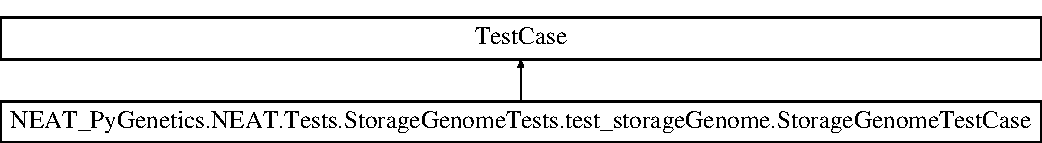
\includegraphics[height=1.927711cm]{classNEAT__PyGenetics_1_1NEAT_1_1Tests_1_1StorageGenomeTests_1_1test__storageGenome_1_1StorageGenomeTestCase}
\end{center}
\end{figure}
\subsection*{Public Member Functions}
\begin{DoxyCompactItemize}
\item 
def \hyperlink{classNEAT__PyGenetics_1_1NEAT_1_1Tests_1_1StorageGenomeTests_1_1test__storageGenome_1_1StorageGenomeTestCase_a27b58493e931470520a1e71e514009cb}{test\+\_\+eq} (self)
\begin{DoxyCompactList}\small\item\em \hyperlink{namespaceNEAT__PyGenetics_1_1NEAT_1_1Tests}{Tests}, that the equality operator works. \end{DoxyCompactList}\item 
def \hyperlink{classNEAT__PyGenetics_1_1NEAT_1_1Tests_1_1StorageGenomeTests_1_1test__storageGenome_1_1StorageGenomeTestCase_a01f81b00e989464c932df722135daf5c}{test\+\_\+not\+Eq} (self)
\item 
def \hyperlink{classNEAT__PyGenetics_1_1NEAT_1_1Tests_1_1StorageGenomeTests_1_1test__storageGenome_1_1StorageGenomeTestCase_a4c670f9b3e78d2be50280880f1de23d5}{test\+\_\+copy\+Construct} (self)
\end{DoxyCompactItemize}


\subsection{Member Function Documentation}
\index{N\+E\+A\+T\+\_\+\+Py\+Genetics\+::\+N\+E\+A\+T\+::\+Tests\+::\+Storage\+Genome\+Tests\+::test\+\_\+storage\+Genome\+::\+Storage\+Genome\+Test\+Case@{N\+E\+A\+T\+\_\+\+Py\+Genetics\+::\+N\+E\+A\+T\+::\+Tests\+::\+Storage\+Genome\+Tests\+::test\+\_\+storage\+Genome\+::\+Storage\+Genome\+Test\+Case}!test\+\_\+copy\+Construct@{test\+\_\+copy\+Construct}}
\index{test\+\_\+copy\+Construct@{test\+\_\+copy\+Construct}!N\+E\+A\+T\+\_\+\+Py\+Genetics\+::\+N\+E\+A\+T\+::\+Tests\+::\+Storage\+Genome\+Tests\+::test\+\_\+storage\+Genome\+::\+Storage\+Genome\+Test\+Case@{N\+E\+A\+T\+\_\+\+Py\+Genetics\+::\+N\+E\+A\+T\+::\+Tests\+::\+Storage\+Genome\+Tests\+::test\+\_\+storage\+Genome\+::\+Storage\+Genome\+Test\+Case}}
\subsubsection[{\texorpdfstring{test\+\_\+copy\+Construct(self)}{test_copyConstruct(self)}}]{\setlength{\rightskip}{0pt plus 5cm}def N\+E\+A\+T\+\_\+\+Py\+Genetics.\+N\+E\+A\+T.\+Tests.\+Storage\+Genome\+Tests.\+test\+\_\+storage\+Genome.\+Storage\+Genome\+Test\+Case.\+test\+\_\+copy\+Construct (
\begin{DoxyParamCaption}
\item[{}]{self}
\end{DoxyParamCaption}
)}\hypertarget{classNEAT__PyGenetics_1_1NEAT_1_1Tests_1_1StorageGenomeTests_1_1test__storageGenome_1_1StorageGenomeTestCase_a4c670f9b3e78d2be50280880f1de23d5}{}\label{classNEAT__PyGenetics_1_1NEAT_1_1Tests_1_1StorageGenomeTests_1_1test__storageGenome_1_1StorageGenomeTestCase_a4c670f9b3e78d2be50280880f1de23d5}
\index{N\+E\+A\+T\+\_\+\+Py\+Genetics\+::\+N\+E\+A\+T\+::\+Tests\+::\+Storage\+Genome\+Tests\+::test\+\_\+storage\+Genome\+::\+Storage\+Genome\+Test\+Case@{N\+E\+A\+T\+\_\+\+Py\+Genetics\+::\+N\+E\+A\+T\+::\+Tests\+::\+Storage\+Genome\+Tests\+::test\+\_\+storage\+Genome\+::\+Storage\+Genome\+Test\+Case}!test\+\_\+eq@{test\+\_\+eq}}
\index{test\+\_\+eq@{test\+\_\+eq}!N\+E\+A\+T\+\_\+\+Py\+Genetics\+::\+N\+E\+A\+T\+::\+Tests\+::\+Storage\+Genome\+Tests\+::test\+\_\+storage\+Genome\+::\+Storage\+Genome\+Test\+Case@{N\+E\+A\+T\+\_\+\+Py\+Genetics\+::\+N\+E\+A\+T\+::\+Tests\+::\+Storage\+Genome\+Tests\+::test\+\_\+storage\+Genome\+::\+Storage\+Genome\+Test\+Case}}
\subsubsection[{\texorpdfstring{test\+\_\+eq(self)}{test_eq(self)}}]{\setlength{\rightskip}{0pt plus 5cm}def N\+E\+A\+T\+\_\+\+Py\+Genetics.\+N\+E\+A\+T.\+Tests.\+Storage\+Genome\+Tests.\+test\+\_\+storage\+Genome.\+Storage\+Genome\+Test\+Case.\+test\+\_\+eq (
\begin{DoxyParamCaption}
\item[{}]{self}
\end{DoxyParamCaption}
)}\hypertarget{classNEAT__PyGenetics_1_1NEAT_1_1Tests_1_1StorageGenomeTests_1_1test__storageGenome_1_1StorageGenomeTestCase_a27b58493e931470520a1e71e514009cb}{}\label{classNEAT__PyGenetics_1_1NEAT_1_1Tests_1_1StorageGenomeTests_1_1test__storageGenome_1_1StorageGenomeTestCase_a27b58493e931470520a1e71e514009cb}


\hyperlink{namespaceNEAT__PyGenetics_1_1NEAT_1_1Tests}{Tests}, that the equality operator works. 

\+:return\+: \index{N\+E\+A\+T\+\_\+\+Py\+Genetics\+::\+N\+E\+A\+T\+::\+Tests\+::\+Storage\+Genome\+Tests\+::test\+\_\+storage\+Genome\+::\+Storage\+Genome\+Test\+Case@{N\+E\+A\+T\+\_\+\+Py\+Genetics\+::\+N\+E\+A\+T\+::\+Tests\+::\+Storage\+Genome\+Tests\+::test\+\_\+storage\+Genome\+::\+Storage\+Genome\+Test\+Case}!test\+\_\+not\+Eq@{test\+\_\+not\+Eq}}
\index{test\+\_\+not\+Eq@{test\+\_\+not\+Eq}!N\+E\+A\+T\+\_\+\+Py\+Genetics\+::\+N\+E\+A\+T\+::\+Tests\+::\+Storage\+Genome\+Tests\+::test\+\_\+storage\+Genome\+::\+Storage\+Genome\+Test\+Case@{N\+E\+A\+T\+\_\+\+Py\+Genetics\+::\+N\+E\+A\+T\+::\+Tests\+::\+Storage\+Genome\+Tests\+::test\+\_\+storage\+Genome\+::\+Storage\+Genome\+Test\+Case}}
\subsubsection[{\texorpdfstring{test\+\_\+not\+Eq(self)}{test_notEq(self)}}]{\setlength{\rightskip}{0pt plus 5cm}def N\+E\+A\+T\+\_\+\+Py\+Genetics.\+N\+E\+A\+T.\+Tests.\+Storage\+Genome\+Tests.\+test\+\_\+storage\+Genome.\+Storage\+Genome\+Test\+Case.\+test\+\_\+not\+Eq (
\begin{DoxyParamCaption}
\item[{}]{self}
\end{DoxyParamCaption}
)}\hypertarget{classNEAT__PyGenetics_1_1NEAT_1_1Tests_1_1StorageGenomeTests_1_1test__storageGenome_1_1StorageGenomeTestCase_a01f81b00e989464c932df722135daf5c}{}\label{classNEAT__PyGenetics_1_1NEAT_1_1Tests_1_1StorageGenomeTests_1_1test__storageGenome_1_1StorageGenomeTestCase_a01f81b00e989464c932df722135daf5c}


The documentation for this class was generated from the following file\+:\begin{DoxyCompactItemize}
\item 
N\+E\+A\+T/\+Tests/\+Storage\+Genome\+Tests/\hyperlink{test__storageGenome_8py}{test\+\_\+storage\+Genome.\+py}\end{DoxyCompactItemize}

\hypertarget{classNEAT__PyGenetics_1_1NEAT_1_1Tests_1_1AnalystTests_1_1test__genomeSelector_1_1test__genomeSelector}{}\section{N\+E\+A\+T\+\_\+\+Py\+Genetics.\+N\+E\+A\+T.\+Tests.\+Analyst\+Tests.\+test\+\_\+genome\+Selector.\+test\+\_\+genome\+Selector Class Reference}
\label{classNEAT__PyGenetics_1_1NEAT_1_1Tests_1_1AnalystTests_1_1test__genomeSelector_1_1test__genomeSelector}\index{N\+E\+A\+T\+\_\+\+Py\+Genetics.\+N\+E\+A\+T.\+Tests.\+Analyst\+Tests.\+test\+\_\+genome\+Selector.\+test\+\_\+genome\+Selector@{N\+E\+A\+T\+\_\+\+Py\+Genetics.\+N\+E\+A\+T.\+Tests.\+Analyst\+Tests.\+test\+\_\+genome\+Selector.\+test\+\_\+genome\+Selector}}
Inheritance diagram for N\+E\+A\+T\+\_\+\+Py\+Genetics.\+N\+E\+A\+T.\+Tests.\+Analyst\+Tests.\+test\+\_\+genome\+Selector.\+test\+\_\+genome\+Selector\+:\begin{figure}[H]
\begin{center}
\leavevmode
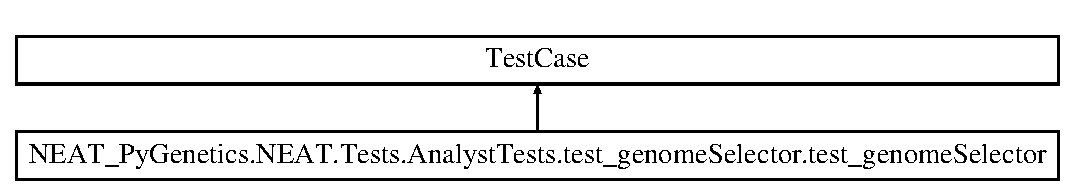
\includegraphics[height=2.000000cm]{classNEAT__PyGenetics_1_1NEAT_1_1Tests_1_1AnalystTests_1_1test__genomeSelector_1_1test__genomeSelector}
\end{center}
\end{figure}
\subsection*{Public Member Functions}
\begin{DoxyCompactItemize}
\item 
def \hyperlink{classNEAT__PyGenetics_1_1NEAT_1_1Tests_1_1AnalystTests_1_1test__genomeSelector_1_1test__genomeSelector_a73634e74c61c8367095ed89b1a9ffa8d}{set\+Up} (self)
\item 
def \hyperlink{classNEAT__PyGenetics_1_1NEAT_1_1Tests_1_1AnalystTests_1_1test__genomeSelector_1_1test__genomeSelector_abf45d8dbc127efe9b7a89415b2f0b605}{test\+\_\+get\+Genomes\+In\+Cluster} (self)
\item 
def \hyperlink{classNEAT__PyGenetics_1_1NEAT_1_1Tests_1_1AnalystTests_1_1test__genomeSelector_1_1test__genomeSelector_a845cb361d31d78f62c573610a01c9c52}{test\+\_\+get\+Cluster\+Area\+Sorted\+By\+Fitness} (self)
\item 
def \hyperlink{classNEAT__PyGenetics_1_1NEAT_1_1Tests_1_1AnalystTests_1_1test__genomeSelector_1_1test__genomeSelector_abe868724b36a1423c915ca001bdfacb7}{test\+\_\+select\+Genomes\+For\+Breeding\+\_\+and\+\_\+select\+Genomes\+For\+Mutation} (self)
\item 
def \hyperlink{classNEAT__PyGenetics_1_1NEAT_1_1Tests_1_1AnalystTests_1_1test__genomeSelector_1_1test__genomeSelector_a02f6228ac878117e968633e7d0652e37}{test\+\_\+select\+Cluster\+For\+Combination} (self)
\item 
def \hyperlink{classNEAT__PyGenetics_1_1NEAT_1_1Tests_1_1AnalystTests_1_1test__genomeSelector_1_1test__genomeSelector_a1a32ff097226fd39d70886ef046293d4}{test\+\_\+select\+Cluster\+Combination} (self)
\item 
def \hyperlink{classNEAT__PyGenetics_1_1NEAT_1_1Tests_1_1AnalystTests_1_1test__genomeSelector_1_1test__genomeSelector_a5c10235f34e1e4e56e06ad1c17d787c5}{test\+\_\+select\+Genomes\+For\+Discarding} (self)
\begin{DoxyCompactList}\small\item\em checks if 20\% of worst cluster or genomes were selected \+:return\+: \end{DoxyCompactList}\end{DoxyCompactItemize}
\subsection*{Public Attributes}
\begin{DoxyCompactItemize}
\item 
\hyperlink{classNEAT__PyGenetics_1_1NEAT_1_1Tests_1_1AnalystTests_1_1test__genomeSelector_1_1test__genomeSelector_af28f36e08d36b7693e8d181ee8143751}{mock\+\_\+genome\+\_\+repository}
\item 
\hyperlink{classNEAT__PyGenetics_1_1NEAT_1_1Tests_1_1AnalystTests_1_1test__genomeSelector_1_1test__genomeSelector_a54e3883498756f3e673b2eebc77890cb}{mock\+\_\+cluster\+\_\+repository}
\item 
\hyperlink{classNEAT__PyGenetics_1_1NEAT_1_1Tests_1_1AnalystTests_1_1test__genomeSelector_1_1test__genomeSelector_ac77001932f6d9ab981a690257f7ff5d1}{mock\+\_\+selection\+\_\+parameters}
\item 
\hyperlink{classNEAT__PyGenetics_1_1NEAT_1_1Tests_1_1AnalystTests_1_1test__genomeSelector_1_1test__genomeSelector_a824c9616385543a8e9fe05a641932676}{genome\+\_\+selector}
\end{DoxyCompactItemize}


\subsection{Member Function Documentation}
\index{N\+E\+A\+T\+\_\+\+Py\+Genetics\+::\+N\+E\+A\+T\+::\+Tests\+::\+Analyst\+Tests\+::test\+\_\+genome\+Selector\+::test\+\_\+genome\+Selector@{N\+E\+A\+T\+\_\+\+Py\+Genetics\+::\+N\+E\+A\+T\+::\+Tests\+::\+Analyst\+Tests\+::test\+\_\+genome\+Selector\+::test\+\_\+genome\+Selector}!set\+Up@{set\+Up}}
\index{set\+Up@{set\+Up}!N\+E\+A\+T\+\_\+\+Py\+Genetics\+::\+N\+E\+A\+T\+::\+Tests\+::\+Analyst\+Tests\+::test\+\_\+genome\+Selector\+::test\+\_\+genome\+Selector@{N\+E\+A\+T\+\_\+\+Py\+Genetics\+::\+N\+E\+A\+T\+::\+Tests\+::\+Analyst\+Tests\+::test\+\_\+genome\+Selector\+::test\+\_\+genome\+Selector}}
\subsubsection[{\texorpdfstring{set\+Up(self)}{setUp(self)}}]{\setlength{\rightskip}{0pt plus 5cm}def N\+E\+A\+T\+\_\+\+Py\+Genetics.\+N\+E\+A\+T.\+Tests.\+Analyst\+Tests.\+test\+\_\+genome\+Selector.\+test\+\_\+genome\+Selector.\+set\+Up (
\begin{DoxyParamCaption}
\item[{}]{self}
\end{DoxyParamCaption}
)}\hypertarget{classNEAT__PyGenetics_1_1NEAT_1_1Tests_1_1AnalystTests_1_1test__genomeSelector_1_1test__genomeSelector_a73634e74c61c8367095ed89b1a9ffa8d}{}\label{classNEAT__PyGenetics_1_1NEAT_1_1Tests_1_1AnalystTests_1_1test__genomeSelector_1_1test__genomeSelector_a73634e74c61c8367095ed89b1a9ffa8d}
\index{N\+E\+A\+T\+\_\+\+Py\+Genetics\+::\+N\+E\+A\+T\+::\+Tests\+::\+Analyst\+Tests\+::test\+\_\+genome\+Selector\+::test\+\_\+genome\+Selector@{N\+E\+A\+T\+\_\+\+Py\+Genetics\+::\+N\+E\+A\+T\+::\+Tests\+::\+Analyst\+Tests\+::test\+\_\+genome\+Selector\+::test\+\_\+genome\+Selector}!test\+\_\+get\+Cluster\+Area\+Sorted\+By\+Fitness@{test\+\_\+get\+Cluster\+Area\+Sorted\+By\+Fitness}}
\index{test\+\_\+get\+Cluster\+Area\+Sorted\+By\+Fitness@{test\+\_\+get\+Cluster\+Area\+Sorted\+By\+Fitness}!N\+E\+A\+T\+\_\+\+Py\+Genetics\+::\+N\+E\+A\+T\+::\+Tests\+::\+Analyst\+Tests\+::test\+\_\+genome\+Selector\+::test\+\_\+genome\+Selector@{N\+E\+A\+T\+\_\+\+Py\+Genetics\+::\+N\+E\+A\+T\+::\+Tests\+::\+Analyst\+Tests\+::test\+\_\+genome\+Selector\+::test\+\_\+genome\+Selector}}
\subsubsection[{\texorpdfstring{test\+\_\+get\+Cluster\+Area\+Sorted\+By\+Fitness(self)}{test_getClusterAreaSortedByFitness(self)}}]{\setlength{\rightskip}{0pt plus 5cm}def N\+E\+A\+T\+\_\+\+Py\+Genetics.\+N\+E\+A\+T.\+Tests.\+Analyst\+Tests.\+test\+\_\+genome\+Selector.\+test\+\_\+genome\+Selector.\+test\+\_\+get\+Cluster\+Area\+Sorted\+By\+Fitness (
\begin{DoxyParamCaption}
\item[{}]{self}
\end{DoxyParamCaption}
)}\hypertarget{classNEAT__PyGenetics_1_1NEAT_1_1Tests_1_1AnalystTests_1_1test__genomeSelector_1_1test__genomeSelector_a845cb361d31d78f62c573610a01c9c52}{}\label{classNEAT__PyGenetics_1_1NEAT_1_1Tests_1_1AnalystTests_1_1test__genomeSelector_1_1test__genomeSelector_a845cb361d31d78f62c573610a01c9c52}
\index{N\+E\+A\+T\+\_\+\+Py\+Genetics\+::\+N\+E\+A\+T\+::\+Tests\+::\+Analyst\+Tests\+::test\+\_\+genome\+Selector\+::test\+\_\+genome\+Selector@{N\+E\+A\+T\+\_\+\+Py\+Genetics\+::\+N\+E\+A\+T\+::\+Tests\+::\+Analyst\+Tests\+::test\+\_\+genome\+Selector\+::test\+\_\+genome\+Selector}!test\+\_\+get\+Genomes\+In\+Cluster@{test\+\_\+get\+Genomes\+In\+Cluster}}
\index{test\+\_\+get\+Genomes\+In\+Cluster@{test\+\_\+get\+Genomes\+In\+Cluster}!N\+E\+A\+T\+\_\+\+Py\+Genetics\+::\+N\+E\+A\+T\+::\+Tests\+::\+Analyst\+Tests\+::test\+\_\+genome\+Selector\+::test\+\_\+genome\+Selector@{N\+E\+A\+T\+\_\+\+Py\+Genetics\+::\+N\+E\+A\+T\+::\+Tests\+::\+Analyst\+Tests\+::test\+\_\+genome\+Selector\+::test\+\_\+genome\+Selector}}
\subsubsection[{\texorpdfstring{test\+\_\+get\+Genomes\+In\+Cluster(self)}{test_getGenomesInCluster(self)}}]{\setlength{\rightskip}{0pt plus 5cm}def N\+E\+A\+T\+\_\+\+Py\+Genetics.\+N\+E\+A\+T.\+Tests.\+Analyst\+Tests.\+test\+\_\+genome\+Selector.\+test\+\_\+genome\+Selector.\+test\+\_\+get\+Genomes\+In\+Cluster (
\begin{DoxyParamCaption}
\item[{}]{self}
\end{DoxyParamCaption}
)}\hypertarget{classNEAT__PyGenetics_1_1NEAT_1_1Tests_1_1AnalystTests_1_1test__genomeSelector_1_1test__genomeSelector_abf45d8dbc127efe9b7a89415b2f0b605}{}\label{classNEAT__PyGenetics_1_1NEAT_1_1Tests_1_1AnalystTests_1_1test__genomeSelector_1_1test__genomeSelector_abf45d8dbc127efe9b7a89415b2f0b605}
\index{N\+E\+A\+T\+\_\+\+Py\+Genetics\+::\+N\+E\+A\+T\+::\+Tests\+::\+Analyst\+Tests\+::test\+\_\+genome\+Selector\+::test\+\_\+genome\+Selector@{N\+E\+A\+T\+\_\+\+Py\+Genetics\+::\+N\+E\+A\+T\+::\+Tests\+::\+Analyst\+Tests\+::test\+\_\+genome\+Selector\+::test\+\_\+genome\+Selector}!test\+\_\+select\+Cluster\+Combination@{test\+\_\+select\+Cluster\+Combination}}
\index{test\+\_\+select\+Cluster\+Combination@{test\+\_\+select\+Cluster\+Combination}!N\+E\+A\+T\+\_\+\+Py\+Genetics\+::\+N\+E\+A\+T\+::\+Tests\+::\+Analyst\+Tests\+::test\+\_\+genome\+Selector\+::test\+\_\+genome\+Selector@{N\+E\+A\+T\+\_\+\+Py\+Genetics\+::\+N\+E\+A\+T\+::\+Tests\+::\+Analyst\+Tests\+::test\+\_\+genome\+Selector\+::test\+\_\+genome\+Selector}}
\subsubsection[{\texorpdfstring{test\+\_\+select\+Cluster\+Combination(self)}{test_selectClusterCombination(self)}}]{\setlength{\rightskip}{0pt plus 5cm}def N\+E\+A\+T\+\_\+\+Py\+Genetics.\+N\+E\+A\+T.\+Tests.\+Analyst\+Tests.\+test\+\_\+genome\+Selector.\+test\+\_\+genome\+Selector.\+test\+\_\+select\+Cluster\+Combination (
\begin{DoxyParamCaption}
\item[{}]{self}
\end{DoxyParamCaption}
)}\hypertarget{classNEAT__PyGenetics_1_1NEAT_1_1Tests_1_1AnalystTests_1_1test__genomeSelector_1_1test__genomeSelector_a1a32ff097226fd39d70886ef046293d4}{}\label{classNEAT__PyGenetics_1_1NEAT_1_1Tests_1_1AnalystTests_1_1test__genomeSelector_1_1test__genomeSelector_a1a32ff097226fd39d70886ef046293d4}
\index{N\+E\+A\+T\+\_\+\+Py\+Genetics\+::\+N\+E\+A\+T\+::\+Tests\+::\+Analyst\+Tests\+::test\+\_\+genome\+Selector\+::test\+\_\+genome\+Selector@{N\+E\+A\+T\+\_\+\+Py\+Genetics\+::\+N\+E\+A\+T\+::\+Tests\+::\+Analyst\+Tests\+::test\+\_\+genome\+Selector\+::test\+\_\+genome\+Selector}!test\+\_\+select\+Cluster\+For\+Combination@{test\+\_\+select\+Cluster\+For\+Combination}}
\index{test\+\_\+select\+Cluster\+For\+Combination@{test\+\_\+select\+Cluster\+For\+Combination}!N\+E\+A\+T\+\_\+\+Py\+Genetics\+::\+N\+E\+A\+T\+::\+Tests\+::\+Analyst\+Tests\+::test\+\_\+genome\+Selector\+::test\+\_\+genome\+Selector@{N\+E\+A\+T\+\_\+\+Py\+Genetics\+::\+N\+E\+A\+T\+::\+Tests\+::\+Analyst\+Tests\+::test\+\_\+genome\+Selector\+::test\+\_\+genome\+Selector}}
\subsubsection[{\texorpdfstring{test\+\_\+select\+Cluster\+For\+Combination(self)}{test_selectClusterForCombination(self)}}]{\setlength{\rightskip}{0pt plus 5cm}def N\+E\+A\+T\+\_\+\+Py\+Genetics.\+N\+E\+A\+T.\+Tests.\+Analyst\+Tests.\+test\+\_\+genome\+Selector.\+test\+\_\+genome\+Selector.\+test\+\_\+select\+Cluster\+For\+Combination (
\begin{DoxyParamCaption}
\item[{}]{self}
\end{DoxyParamCaption}
)}\hypertarget{classNEAT__PyGenetics_1_1NEAT_1_1Tests_1_1AnalystTests_1_1test__genomeSelector_1_1test__genomeSelector_a02f6228ac878117e968633e7d0652e37}{}\label{classNEAT__PyGenetics_1_1NEAT_1_1Tests_1_1AnalystTests_1_1test__genomeSelector_1_1test__genomeSelector_a02f6228ac878117e968633e7d0652e37}
\index{N\+E\+A\+T\+\_\+\+Py\+Genetics\+::\+N\+E\+A\+T\+::\+Tests\+::\+Analyst\+Tests\+::test\+\_\+genome\+Selector\+::test\+\_\+genome\+Selector@{N\+E\+A\+T\+\_\+\+Py\+Genetics\+::\+N\+E\+A\+T\+::\+Tests\+::\+Analyst\+Tests\+::test\+\_\+genome\+Selector\+::test\+\_\+genome\+Selector}!test\+\_\+select\+Genomes\+For\+Breeding\+\_\+and\+\_\+select\+Genomes\+For\+Mutation@{test\+\_\+select\+Genomes\+For\+Breeding\+\_\+and\+\_\+select\+Genomes\+For\+Mutation}}
\index{test\+\_\+select\+Genomes\+For\+Breeding\+\_\+and\+\_\+select\+Genomes\+For\+Mutation@{test\+\_\+select\+Genomes\+For\+Breeding\+\_\+and\+\_\+select\+Genomes\+For\+Mutation}!N\+E\+A\+T\+\_\+\+Py\+Genetics\+::\+N\+E\+A\+T\+::\+Tests\+::\+Analyst\+Tests\+::test\+\_\+genome\+Selector\+::test\+\_\+genome\+Selector@{N\+E\+A\+T\+\_\+\+Py\+Genetics\+::\+N\+E\+A\+T\+::\+Tests\+::\+Analyst\+Tests\+::test\+\_\+genome\+Selector\+::test\+\_\+genome\+Selector}}
\subsubsection[{\texorpdfstring{test\+\_\+select\+Genomes\+For\+Breeding\+\_\+and\+\_\+select\+Genomes\+For\+Mutation(self)}{test_selectGenomesForBreeding_and_selectGenomesForMutation(self)}}]{\setlength{\rightskip}{0pt plus 5cm}def N\+E\+A\+T\+\_\+\+Py\+Genetics.\+N\+E\+A\+T.\+Tests.\+Analyst\+Tests.\+test\+\_\+genome\+Selector.\+test\+\_\+genome\+Selector.\+test\+\_\+select\+Genomes\+For\+Breeding\+\_\+and\+\_\+select\+Genomes\+For\+Mutation (
\begin{DoxyParamCaption}
\item[{}]{self}
\end{DoxyParamCaption}
)}\hypertarget{classNEAT__PyGenetics_1_1NEAT_1_1Tests_1_1AnalystTests_1_1test__genomeSelector_1_1test__genomeSelector_abe868724b36a1423c915ca001bdfacb7}{}\label{classNEAT__PyGenetics_1_1NEAT_1_1Tests_1_1AnalystTests_1_1test__genomeSelector_1_1test__genomeSelector_abe868724b36a1423c915ca001bdfacb7}
\index{N\+E\+A\+T\+\_\+\+Py\+Genetics\+::\+N\+E\+A\+T\+::\+Tests\+::\+Analyst\+Tests\+::test\+\_\+genome\+Selector\+::test\+\_\+genome\+Selector@{N\+E\+A\+T\+\_\+\+Py\+Genetics\+::\+N\+E\+A\+T\+::\+Tests\+::\+Analyst\+Tests\+::test\+\_\+genome\+Selector\+::test\+\_\+genome\+Selector}!test\+\_\+select\+Genomes\+For\+Discarding@{test\+\_\+select\+Genomes\+For\+Discarding}}
\index{test\+\_\+select\+Genomes\+For\+Discarding@{test\+\_\+select\+Genomes\+For\+Discarding}!N\+E\+A\+T\+\_\+\+Py\+Genetics\+::\+N\+E\+A\+T\+::\+Tests\+::\+Analyst\+Tests\+::test\+\_\+genome\+Selector\+::test\+\_\+genome\+Selector@{N\+E\+A\+T\+\_\+\+Py\+Genetics\+::\+N\+E\+A\+T\+::\+Tests\+::\+Analyst\+Tests\+::test\+\_\+genome\+Selector\+::test\+\_\+genome\+Selector}}
\subsubsection[{\texorpdfstring{test\+\_\+select\+Genomes\+For\+Discarding(self)}{test_selectGenomesForDiscarding(self)}}]{\setlength{\rightskip}{0pt plus 5cm}def N\+E\+A\+T\+\_\+\+Py\+Genetics.\+N\+E\+A\+T.\+Tests.\+Analyst\+Tests.\+test\+\_\+genome\+Selector.\+test\+\_\+genome\+Selector.\+test\+\_\+select\+Genomes\+For\+Discarding (
\begin{DoxyParamCaption}
\item[{}]{self}
\end{DoxyParamCaption}
)}\hypertarget{classNEAT__PyGenetics_1_1NEAT_1_1Tests_1_1AnalystTests_1_1test__genomeSelector_1_1test__genomeSelector_a5c10235f34e1e4e56e06ad1c17d787c5}{}\label{classNEAT__PyGenetics_1_1NEAT_1_1Tests_1_1AnalystTests_1_1test__genomeSelector_1_1test__genomeSelector_a5c10235f34e1e4e56e06ad1c17d787c5}


checks if 20\% of worst cluster or genomes were selected \+:return\+: 



\subsection{Member Data Documentation}
\index{N\+E\+A\+T\+\_\+\+Py\+Genetics\+::\+N\+E\+A\+T\+::\+Tests\+::\+Analyst\+Tests\+::test\+\_\+genome\+Selector\+::test\+\_\+genome\+Selector@{N\+E\+A\+T\+\_\+\+Py\+Genetics\+::\+N\+E\+A\+T\+::\+Tests\+::\+Analyst\+Tests\+::test\+\_\+genome\+Selector\+::test\+\_\+genome\+Selector}!genome\+\_\+selector@{genome\+\_\+selector}}
\index{genome\+\_\+selector@{genome\+\_\+selector}!N\+E\+A\+T\+\_\+\+Py\+Genetics\+::\+N\+E\+A\+T\+::\+Tests\+::\+Analyst\+Tests\+::test\+\_\+genome\+Selector\+::test\+\_\+genome\+Selector@{N\+E\+A\+T\+\_\+\+Py\+Genetics\+::\+N\+E\+A\+T\+::\+Tests\+::\+Analyst\+Tests\+::test\+\_\+genome\+Selector\+::test\+\_\+genome\+Selector}}
\subsubsection[{\texorpdfstring{genome\+\_\+selector}{genome_selector}}]{\setlength{\rightskip}{0pt plus 5cm}N\+E\+A\+T\+\_\+\+Py\+Genetics.\+N\+E\+A\+T.\+Tests.\+Analyst\+Tests.\+test\+\_\+genome\+Selector.\+test\+\_\+genome\+Selector.\+genome\+\_\+selector}\hypertarget{classNEAT__PyGenetics_1_1NEAT_1_1Tests_1_1AnalystTests_1_1test__genomeSelector_1_1test__genomeSelector_a824c9616385543a8e9fe05a641932676}{}\label{classNEAT__PyGenetics_1_1NEAT_1_1Tests_1_1AnalystTests_1_1test__genomeSelector_1_1test__genomeSelector_a824c9616385543a8e9fe05a641932676}
\index{N\+E\+A\+T\+\_\+\+Py\+Genetics\+::\+N\+E\+A\+T\+::\+Tests\+::\+Analyst\+Tests\+::test\+\_\+genome\+Selector\+::test\+\_\+genome\+Selector@{N\+E\+A\+T\+\_\+\+Py\+Genetics\+::\+N\+E\+A\+T\+::\+Tests\+::\+Analyst\+Tests\+::test\+\_\+genome\+Selector\+::test\+\_\+genome\+Selector}!mock\+\_\+cluster\+\_\+repository@{mock\+\_\+cluster\+\_\+repository}}
\index{mock\+\_\+cluster\+\_\+repository@{mock\+\_\+cluster\+\_\+repository}!N\+E\+A\+T\+\_\+\+Py\+Genetics\+::\+N\+E\+A\+T\+::\+Tests\+::\+Analyst\+Tests\+::test\+\_\+genome\+Selector\+::test\+\_\+genome\+Selector@{N\+E\+A\+T\+\_\+\+Py\+Genetics\+::\+N\+E\+A\+T\+::\+Tests\+::\+Analyst\+Tests\+::test\+\_\+genome\+Selector\+::test\+\_\+genome\+Selector}}
\subsubsection[{\texorpdfstring{mock\+\_\+cluster\+\_\+repository}{mock_cluster_repository}}]{\setlength{\rightskip}{0pt plus 5cm}N\+E\+A\+T\+\_\+\+Py\+Genetics.\+N\+E\+A\+T.\+Tests.\+Analyst\+Tests.\+test\+\_\+genome\+Selector.\+test\+\_\+genome\+Selector.\+mock\+\_\+cluster\+\_\+repository}\hypertarget{classNEAT__PyGenetics_1_1NEAT_1_1Tests_1_1AnalystTests_1_1test__genomeSelector_1_1test__genomeSelector_a54e3883498756f3e673b2eebc77890cb}{}\label{classNEAT__PyGenetics_1_1NEAT_1_1Tests_1_1AnalystTests_1_1test__genomeSelector_1_1test__genomeSelector_a54e3883498756f3e673b2eebc77890cb}
\index{N\+E\+A\+T\+\_\+\+Py\+Genetics\+::\+N\+E\+A\+T\+::\+Tests\+::\+Analyst\+Tests\+::test\+\_\+genome\+Selector\+::test\+\_\+genome\+Selector@{N\+E\+A\+T\+\_\+\+Py\+Genetics\+::\+N\+E\+A\+T\+::\+Tests\+::\+Analyst\+Tests\+::test\+\_\+genome\+Selector\+::test\+\_\+genome\+Selector}!mock\+\_\+genome\+\_\+repository@{mock\+\_\+genome\+\_\+repository}}
\index{mock\+\_\+genome\+\_\+repository@{mock\+\_\+genome\+\_\+repository}!N\+E\+A\+T\+\_\+\+Py\+Genetics\+::\+N\+E\+A\+T\+::\+Tests\+::\+Analyst\+Tests\+::test\+\_\+genome\+Selector\+::test\+\_\+genome\+Selector@{N\+E\+A\+T\+\_\+\+Py\+Genetics\+::\+N\+E\+A\+T\+::\+Tests\+::\+Analyst\+Tests\+::test\+\_\+genome\+Selector\+::test\+\_\+genome\+Selector}}
\subsubsection[{\texorpdfstring{mock\+\_\+genome\+\_\+repository}{mock_genome_repository}}]{\setlength{\rightskip}{0pt plus 5cm}N\+E\+A\+T\+\_\+\+Py\+Genetics.\+N\+E\+A\+T.\+Tests.\+Analyst\+Tests.\+test\+\_\+genome\+Selector.\+test\+\_\+genome\+Selector.\+mock\+\_\+genome\+\_\+repository}\hypertarget{classNEAT__PyGenetics_1_1NEAT_1_1Tests_1_1AnalystTests_1_1test__genomeSelector_1_1test__genomeSelector_af28f36e08d36b7693e8d181ee8143751}{}\label{classNEAT__PyGenetics_1_1NEAT_1_1Tests_1_1AnalystTests_1_1test__genomeSelector_1_1test__genomeSelector_af28f36e08d36b7693e8d181ee8143751}
\index{N\+E\+A\+T\+\_\+\+Py\+Genetics\+::\+N\+E\+A\+T\+::\+Tests\+::\+Analyst\+Tests\+::test\+\_\+genome\+Selector\+::test\+\_\+genome\+Selector@{N\+E\+A\+T\+\_\+\+Py\+Genetics\+::\+N\+E\+A\+T\+::\+Tests\+::\+Analyst\+Tests\+::test\+\_\+genome\+Selector\+::test\+\_\+genome\+Selector}!mock\+\_\+selection\+\_\+parameters@{mock\+\_\+selection\+\_\+parameters}}
\index{mock\+\_\+selection\+\_\+parameters@{mock\+\_\+selection\+\_\+parameters}!N\+E\+A\+T\+\_\+\+Py\+Genetics\+::\+N\+E\+A\+T\+::\+Tests\+::\+Analyst\+Tests\+::test\+\_\+genome\+Selector\+::test\+\_\+genome\+Selector@{N\+E\+A\+T\+\_\+\+Py\+Genetics\+::\+N\+E\+A\+T\+::\+Tests\+::\+Analyst\+Tests\+::test\+\_\+genome\+Selector\+::test\+\_\+genome\+Selector}}
\subsubsection[{\texorpdfstring{mock\+\_\+selection\+\_\+parameters}{mock_selection_parameters}}]{\setlength{\rightskip}{0pt plus 5cm}N\+E\+A\+T\+\_\+\+Py\+Genetics.\+N\+E\+A\+T.\+Tests.\+Analyst\+Tests.\+test\+\_\+genome\+Selector.\+test\+\_\+genome\+Selector.\+mock\+\_\+selection\+\_\+parameters}\hypertarget{classNEAT__PyGenetics_1_1NEAT_1_1Tests_1_1AnalystTests_1_1test__genomeSelector_1_1test__genomeSelector_ac77001932f6d9ab981a690257f7ff5d1}{}\label{classNEAT__PyGenetics_1_1NEAT_1_1Tests_1_1AnalystTests_1_1test__genomeSelector_1_1test__genomeSelector_ac77001932f6d9ab981a690257f7ff5d1}


The documentation for this class was generated from the following file\+:\begin{DoxyCompactItemize}
\item 
N\+E\+A\+T/\+Tests/\+Analyst\+Tests/\hyperlink{test__genomeSelector_8py}{test\+\_\+genome\+Selector.\+py}\end{DoxyCompactItemize}

\hypertarget{classNEAT__PyGenetics_1_1NEAT_1_1Tests_1_1AnalysisGenomeTests_1_1test__analysisGenome_1_1TestAnalysisGenome}{}\section{N\+E\+A\+T\+\_\+\+Py\+Genetics.\+N\+E\+A\+T.\+Tests.\+Analysis\+Genome\+Tests.\+test\+\_\+analysis\+Genome.\+Test\+Analysis\+Genome Class Reference}
\label{classNEAT__PyGenetics_1_1NEAT_1_1Tests_1_1AnalysisGenomeTests_1_1test__analysisGenome_1_1TestAnalysisGenome}\index{N\+E\+A\+T\+\_\+\+Py\+Genetics.\+N\+E\+A\+T.\+Tests.\+Analysis\+Genome\+Tests.\+test\+\_\+analysis\+Genome.\+Test\+Analysis\+Genome@{N\+E\+A\+T\+\_\+\+Py\+Genetics.\+N\+E\+A\+T.\+Tests.\+Analysis\+Genome\+Tests.\+test\+\_\+analysis\+Genome.\+Test\+Analysis\+Genome}}
Inheritance diagram for N\+E\+A\+T\+\_\+\+Py\+Genetics.\+N\+E\+A\+T.\+Tests.\+Analysis\+Genome\+Tests.\+test\+\_\+analysis\+Genome.\+Test\+Analysis\+Genome\+:\begin{figure}[H]
\begin{center}
\leavevmode
\includegraphics[height=1.985816cm]{classNEAT__PyGenetics_1_1NEAT_1_1Tests_1_1AnalysisGenomeTests_1_1test__analysisGenome_1_1TestAnalysisGenome}
\end{center}
\end{figure}
\subsection*{Public Member Functions}
\begin{DoxyCompactItemize}
\item 
def \hyperlink{classNEAT__PyGenetics_1_1NEAT_1_1Tests_1_1AnalysisGenomeTests_1_1test__analysisGenome_1_1TestAnalysisGenome_a7eb8161235eddea20bc4c9663570cdac}{set\+Up} (self)
\item 
def \hyperlink{classNEAT__PyGenetics_1_1NEAT_1_1Tests_1_1AnalysisGenomeTests_1_1test__analysisGenome_1_1TestAnalysisGenome_ac95b9d78e65bf92e330d9c44ed0ef3fc}{test\+\_\+\+\_\+add\+\_\+node} (self)
\item 
def \hyperlink{classNEAT__PyGenetics_1_1NEAT_1_1Tests_1_1AnalysisGenomeTests_1_1test__analysisGenome_1_1TestAnalysisGenome_aaffe3eb85a13c66e0825223bae4ac78e}{test\+\_\+\+\_\+add\+\_\+edge} (self)
\item 
def \hyperlink{classNEAT__PyGenetics_1_1NEAT_1_1Tests_1_1AnalysisGenomeTests_1_1test__analysisGenome_1_1TestAnalysisGenome_a54eb6e20e337eeb03a7c31ee7339712f}{test\+\_\+\+\_\+add\+\_\+edge\+\_\+without\+\_\+preadded\+\_\+nodes} (self)
\item 
def \hyperlink{classNEAT__PyGenetics_1_1NEAT_1_1Tests_1_1AnalysisGenomeTests_1_1test__analysisGenome_1_1TestAnalysisGenome_a603ac3eb47164d8edb36630a92655adb}{test\+\_\+\+\_\+add\+\_\+edge\+\_\+with\+\_\+preadded\+\_\+source\+\_\+node} (self)
\item 
def \hyperlink{classNEAT__PyGenetics_1_1NEAT_1_1Tests_1_1AnalysisGenomeTests_1_1test__analysisGenome_1_1TestAnalysisGenome_a24febdb8aa6bb2efff1f6dd77b4d4393}{test\+\_\+init\+\_\+from\+\_\+storage\+\_\+structure} (self)
\item 
def \hyperlink{classNEAT__PyGenetics_1_1NEAT_1_1Tests_1_1AnalysisGenomeTests_1_1test__analysisGenome_1_1TestAnalysisGenome_ad10dfce265aa3af67fb951add1fcdd34}{test\+\_\+\+\_\+add\+\_\+input\+\_\+node} (self)
\item 
def \hyperlink{classNEAT__PyGenetics_1_1NEAT_1_1Tests_1_1AnalysisGenomeTests_1_1test__analysisGenome_1_1TestAnalysisGenome_a59b12daf2e5e073af71aa97e0bb87009}{test\+\_\+\+\_\+add\+\_\+output\+\_\+node} (self)
\end{DoxyCompactItemize}
\subsection*{Public Attributes}
\begin{DoxyCompactItemize}
\item 
\hyperlink{classNEAT__PyGenetics_1_1NEAT_1_1Tests_1_1AnalysisGenomeTests_1_1test__analysisGenome_1_1TestAnalysisGenome_a344a0b4458ba026a33e499da5ba58563}{mock\+\_\+gene\+\_\+repository}
\item 
\hyperlink{classNEAT__PyGenetics_1_1NEAT_1_1Tests_1_1AnalysisGenomeTests_1_1test__analysisGenome_1_1TestAnalysisGenome_a422f45a24e190778e830b08d527d2d66}{storage\+\_\+genome}
\end{DoxyCompactItemize}


\subsection{Member Function Documentation}
\index{N\+E\+A\+T\+\_\+\+Py\+Genetics\+::\+N\+E\+A\+T\+::\+Tests\+::\+Analysis\+Genome\+Tests\+::test\+\_\+analysis\+Genome\+::\+Test\+Analysis\+Genome@{N\+E\+A\+T\+\_\+\+Py\+Genetics\+::\+N\+E\+A\+T\+::\+Tests\+::\+Analysis\+Genome\+Tests\+::test\+\_\+analysis\+Genome\+::\+Test\+Analysis\+Genome}!set\+Up@{set\+Up}}
\index{set\+Up@{set\+Up}!N\+E\+A\+T\+\_\+\+Py\+Genetics\+::\+N\+E\+A\+T\+::\+Tests\+::\+Analysis\+Genome\+Tests\+::test\+\_\+analysis\+Genome\+::\+Test\+Analysis\+Genome@{N\+E\+A\+T\+\_\+\+Py\+Genetics\+::\+N\+E\+A\+T\+::\+Tests\+::\+Analysis\+Genome\+Tests\+::test\+\_\+analysis\+Genome\+::\+Test\+Analysis\+Genome}}
\subsubsection[{\texorpdfstring{set\+Up(self)}{setUp(self)}}]{\setlength{\rightskip}{0pt plus 5cm}def N\+E\+A\+T\+\_\+\+Py\+Genetics.\+N\+E\+A\+T.\+Tests.\+Analysis\+Genome\+Tests.\+test\+\_\+analysis\+Genome.\+Test\+Analysis\+Genome.\+set\+Up (
\begin{DoxyParamCaption}
\item[{}]{self}
\end{DoxyParamCaption}
)}\hypertarget{classNEAT__PyGenetics_1_1NEAT_1_1Tests_1_1AnalysisGenomeTests_1_1test__analysisGenome_1_1TestAnalysisGenome_a7eb8161235eddea20bc4c9663570cdac}{}\label{classNEAT__PyGenetics_1_1NEAT_1_1Tests_1_1AnalysisGenomeTests_1_1test__analysisGenome_1_1TestAnalysisGenome_a7eb8161235eddea20bc4c9663570cdac}
\index{N\+E\+A\+T\+\_\+\+Py\+Genetics\+::\+N\+E\+A\+T\+::\+Tests\+::\+Analysis\+Genome\+Tests\+::test\+\_\+analysis\+Genome\+::\+Test\+Analysis\+Genome@{N\+E\+A\+T\+\_\+\+Py\+Genetics\+::\+N\+E\+A\+T\+::\+Tests\+::\+Analysis\+Genome\+Tests\+::test\+\_\+analysis\+Genome\+::\+Test\+Analysis\+Genome}!test\+\_\+\+\_\+add\+\_\+edge@{test\+\_\+\+\_\+add\+\_\+edge}}
\index{test\+\_\+\+\_\+add\+\_\+edge@{test\+\_\+\+\_\+add\+\_\+edge}!N\+E\+A\+T\+\_\+\+Py\+Genetics\+::\+N\+E\+A\+T\+::\+Tests\+::\+Analysis\+Genome\+Tests\+::test\+\_\+analysis\+Genome\+::\+Test\+Analysis\+Genome@{N\+E\+A\+T\+\_\+\+Py\+Genetics\+::\+N\+E\+A\+T\+::\+Tests\+::\+Analysis\+Genome\+Tests\+::test\+\_\+analysis\+Genome\+::\+Test\+Analysis\+Genome}}
\subsubsection[{\texorpdfstring{test\+\_\+\+\_\+add\+\_\+edge(self)}{test__add_edge(self)}}]{\setlength{\rightskip}{0pt plus 5cm}def N\+E\+A\+T\+\_\+\+Py\+Genetics.\+N\+E\+A\+T.\+Tests.\+Analysis\+Genome\+Tests.\+test\+\_\+analysis\+Genome.\+Test\+Analysis\+Genome.\+test\+\_\+\+\_\+add\+\_\+edge (
\begin{DoxyParamCaption}
\item[{}]{self}
\end{DoxyParamCaption}
)}\hypertarget{classNEAT__PyGenetics_1_1NEAT_1_1Tests_1_1AnalysisGenomeTests_1_1test__analysisGenome_1_1TestAnalysisGenome_aaffe3eb85a13c66e0825223bae4ac78e}{}\label{classNEAT__PyGenetics_1_1NEAT_1_1Tests_1_1AnalysisGenomeTests_1_1test__analysisGenome_1_1TestAnalysisGenome_aaffe3eb85a13c66e0825223bae4ac78e}
\index{N\+E\+A\+T\+\_\+\+Py\+Genetics\+::\+N\+E\+A\+T\+::\+Tests\+::\+Analysis\+Genome\+Tests\+::test\+\_\+analysis\+Genome\+::\+Test\+Analysis\+Genome@{N\+E\+A\+T\+\_\+\+Py\+Genetics\+::\+N\+E\+A\+T\+::\+Tests\+::\+Analysis\+Genome\+Tests\+::test\+\_\+analysis\+Genome\+::\+Test\+Analysis\+Genome}!test\+\_\+\+\_\+add\+\_\+edge\+\_\+with\+\_\+preadded\+\_\+source\+\_\+node@{test\+\_\+\+\_\+add\+\_\+edge\+\_\+with\+\_\+preadded\+\_\+source\+\_\+node}}
\index{test\+\_\+\+\_\+add\+\_\+edge\+\_\+with\+\_\+preadded\+\_\+source\+\_\+node@{test\+\_\+\+\_\+add\+\_\+edge\+\_\+with\+\_\+preadded\+\_\+source\+\_\+node}!N\+E\+A\+T\+\_\+\+Py\+Genetics\+::\+N\+E\+A\+T\+::\+Tests\+::\+Analysis\+Genome\+Tests\+::test\+\_\+analysis\+Genome\+::\+Test\+Analysis\+Genome@{N\+E\+A\+T\+\_\+\+Py\+Genetics\+::\+N\+E\+A\+T\+::\+Tests\+::\+Analysis\+Genome\+Tests\+::test\+\_\+analysis\+Genome\+::\+Test\+Analysis\+Genome}}
\subsubsection[{\texorpdfstring{test\+\_\+\+\_\+add\+\_\+edge\+\_\+with\+\_\+preadded\+\_\+source\+\_\+node(self)}{test__add_edge_with_preadded_source_node(self)}}]{\setlength{\rightskip}{0pt plus 5cm}def N\+E\+A\+T\+\_\+\+Py\+Genetics.\+N\+E\+A\+T.\+Tests.\+Analysis\+Genome\+Tests.\+test\+\_\+analysis\+Genome.\+Test\+Analysis\+Genome.\+test\+\_\+\+\_\+add\+\_\+edge\+\_\+with\+\_\+preadded\+\_\+source\+\_\+node (
\begin{DoxyParamCaption}
\item[{}]{self}
\end{DoxyParamCaption}
)}\hypertarget{classNEAT__PyGenetics_1_1NEAT_1_1Tests_1_1AnalysisGenomeTests_1_1test__analysisGenome_1_1TestAnalysisGenome_a603ac3eb47164d8edb36630a92655adb}{}\label{classNEAT__PyGenetics_1_1NEAT_1_1Tests_1_1AnalysisGenomeTests_1_1test__analysisGenome_1_1TestAnalysisGenome_a603ac3eb47164d8edb36630a92655adb}
\index{N\+E\+A\+T\+\_\+\+Py\+Genetics\+::\+N\+E\+A\+T\+::\+Tests\+::\+Analysis\+Genome\+Tests\+::test\+\_\+analysis\+Genome\+::\+Test\+Analysis\+Genome@{N\+E\+A\+T\+\_\+\+Py\+Genetics\+::\+N\+E\+A\+T\+::\+Tests\+::\+Analysis\+Genome\+Tests\+::test\+\_\+analysis\+Genome\+::\+Test\+Analysis\+Genome}!test\+\_\+\+\_\+add\+\_\+edge\+\_\+without\+\_\+preadded\+\_\+nodes@{test\+\_\+\+\_\+add\+\_\+edge\+\_\+without\+\_\+preadded\+\_\+nodes}}
\index{test\+\_\+\+\_\+add\+\_\+edge\+\_\+without\+\_\+preadded\+\_\+nodes@{test\+\_\+\+\_\+add\+\_\+edge\+\_\+without\+\_\+preadded\+\_\+nodes}!N\+E\+A\+T\+\_\+\+Py\+Genetics\+::\+N\+E\+A\+T\+::\+Tests\+::\+Analysis\+Genome\+Tests\+::test\+\_\+analysis\+Genome\+::\+Test\+Analysis\+Genome@{N\+E\+A\+T\+\_\+\+Py\+Genetics\+::\+N\+E\+A\+T\+::\+Tests\+::\+Analysis\+Genome\+Tests\+::test\+\_\+analysis\+Genome\+::\+Test\+Analysis\+Genome}}
\subsubsection[{\texorpdfstring{test\+\_\+\+\_\+add\+\_\+edge\+\_\+without\+\_\+preadded\+\_\+nodes(self)}{test__add_edge_without_preadded_nodes(self)}}]{\setlength{\rightskip}{0pt plus 5cm}def N\+E\+A\+T\+\_\+\+Py\+Genetics.\+N\+E\+A\+T.\+Tests.\+Analysis\+Genome\+Tests.\+test\+\_\+analysis\+Genome.\+Test\+Analysis\+Genome.\+test\+\_\+\+\_\+add\+\_\+edge\+\_\+without\+\_\+preadded\+\_\+nodes (
\begin{DoxyParamCaption}
\item[{}]{self}
\end{DoxyParamCaption}
)}\hypertarget{classNEAT__PyGenetics_1_1NEAT_1_1Tests_1_1AnalysisGenomeTests_1_1test__analysisGenome_1_1TestAnalysisGenome_a54eb6e20e337eeb03a7c31ee7339712f}{}\label{classNEAT__PyGenetics_1_1NEAT_1_1Tests_1_1AnalysisGenomeTests_1_1test__analysisGenome_1_1TestAnalysisGenome_a54eb6e20e337eeb03a7c31ee7339712f}
\index{N\+E\+A\+T\+\_\+\+Py\+Genetics\+::\+N\+E\+A\+T\+::\+Tests\+::\+Analysis\+Genome\+Tests\+::test\+\_\+analysis\+Genome\+::\+Test\+Analysis\+Genome@{N\+E\+A\+T\+\_\+\+Py\+Genetics\+::\+N\+E\+A\+T\+::\+Tests\+::\+Analysis\+Genome\+Tests\+::test\+\_\+analysis\+Genome\+::\+Test\+Analysis\+Genome}!test\+\_\+\+\_\+add\+\_\+input\+\_\+node@{test\+\_\+\+\_\+add\+\_\+input\+\_\+node}}
\index{test\+\_\+\+\_\+add\+\_\+input\+\_\+node@{test\+\_\+\+\_\+add\+\_\+input\+\_\+node}!N\+E\+A\+T\+\_\+\+Py\+Genetics\+::\+N\+E\+A\+T\+::\+Tests\+::\+Analysis\+Genome\+Tests\+::test\+\_\+analysis\+Genome\+::\+Test\+Analysis\+Genome@{N\+E\+A\+T\+\_\+\+Py\+Genetics\+::\+N\+E\+A\+T\+::\+Tests\+::\+Analysis\+Genome\+Tests\+::test\+\_\+analysis\+Genome\+::\+Test\+Analysis\+Genome}}
\subsubsection[{\texorpdfstring{test\+\_\+\+\_\+add\+\_\+input\+\_\+node(self)}{test__add_input_node(self)}}]{\setlength{\rightskip}{0pt plus 5cm}def N\+E\+A\+T\+\_\+\+Py\+Genetics.\+N\+E\+A\+T.\+Tests.\+Analysis\+Genome\+Tests.\+test\+\_\+analysis\+Genome.\+Test\+Analysis\+Genome.\+test\+\_\+\+\_\+add\+\_\+input\+\_\+node (
\begin{DoxyParamCaption}
\item[{}]{self}
\end{DoxyParamCaption}
)}\hypertarget{classNEAT__PyGenetics_1_1NEAT_1_1Tests_1_1AnalysisGenomeTests_1_1test__analysisGenome_1_1TestAnalysisGenome_ad10dfce265aa3af67fb951add1fcdd34}{}\label{classNEAT__PyGenetics_1_1NEAT_1_1Tests_1_1AnalysisGenomeTests_1_1test__analysisGenome_1_1TestAnalysisGenome_ad10dfce265aa3af67fb951add1fcdd34}
\index{N\+E\+A\+T\+\_\+\+Py\+Genetics\+::\+N\+E\+A\+T\+::\+Tests\+::\+Analysis\+Genome\+Tests\+::test\+\_\+analysis\+Genome\+::\+Test\+Analysis\+Genome@{N\+E\+A\+T\+\_\+\+Py\+Genetics\+::\+N\+E\+A\+T\+::\+Tests\+::\+Analysis\+Genome\+Tests\+::test\+\_\+analysis\+Genome\+::\+Test\+Analysis\+Genome}!test\+\_\+\+\_\+add\+\_\+node@{test\+\_\+\+\_\+add\+\_\+node}}
\index{test\+\_\+\+\_\+add\+\_\+node@{test\+\_\+\+\_\+add\+\_\+node}!N\+E\+A\+T\+\_\+\+Py\+Genetics\+::\+N\+E\+A\+T\+::\+Tests\+::\+Analysis\+Genome\+Tests\+::test\+\_\+analysis\+Genome\+::\+Test\+Analysis\+Genome@{N\+E\+A\+T\+\_\+\+Py\+Genetics\+::\+N\+E\+A\+T\+::\+Tests\+::\+Analysis\+Genome\+Tests\+::test\+\_\+analysis\+Genome\+::\+Test\+Analysis\+Genome}}
\subsubsection[{\texorpdfstring{test\+\_\+\+\_\+add\+\_\+node(self)}{test__add_node(self)}}]{\setlength{\rightskip}{0pt plus 5cm}def N\+E\+A\+T\+\_\+\+Py\+Genetics.\+N\+E\+A\+T.\+Tests.\+Analysis\+Genome\+Tests.\+test\+\_\+analysis\+Genome.\+Test\+Analysis\+Genome.\+test\+\_\+\+\_\+add\+\_\+node (
\begin{DoxyParamCaption}
\item[{}]{self}
\end{DoxyParamCaption}
)}\hypertarget{classNEAT__PyGenetics_1_1NEAT_1_1Tests_1_1AnalysisGenomeTests_1_1test__analysisGenome_1_1TestAnalysisGenome_ac95b9d78e65bf92e330d9c44ed0ef3fc}{}\label{classNEAT__PyGenetics_1_1NEAT_1_1Tests_1_1AnalysisGenomeTests_1_1test__analysisGenome_1_1TestAnalysisGenome_ac95b9d78e65bf92e330d9c44ed0ef3fc}
\index{N\+E\+A\+T\+\_\+\+Py\+Genetics\+::\+N\+E\+A\+T\+::\+Tests\+::\+Analysis\+Genome\+Tests\+::test\+\_\+analysis\+Genome\+::\+Test\+Analysis\+Genome@{N\+E\+A\+T\+\_\+\+Py\+Genetics\+::\+N\+E\+A\+T\+::\+Tests\+::\+Analysis\+Genome\+Tests\+::test\+\_\+analysis\+Genome\+::\+Test\+Analysis\+Genome}!test\+\_\+\+\_\+add\+\_\+output\+\_\+node@{test\+\_\+\+\_\+add\+\_\+output\+\_\+node}}
\index{test\+\_\+\+\_\+add\+\_\+output\+\_\+node@{test\+\_\+\+\_\+add\+\_\+output\+\_\+node}!N\+E\+A\+T\+\_\+\+Py\+Genetics\+::\+N\+E\+A\+T\+::\+Tests\+::\+Analysis\+Genome\+Tests\+::test\+\_\+analysis\+Genome\+::\+Test\+Analysis\+Genome@{N\+E\+A\+T\+\_\+\+Py\+Genetics\+::\+N\+E\+A\+T\+::\+Tests\+::\+Analysis\+Genome\+Tests\+::test\+\_\+analysis\+Genome\+::\+Test\+Analysis\+Genome}}
\subsubsection[{\texorpdfstring{test\+\_\+\+\_\+add\+\_\+output\+\_\+node(self)}{test__add_output_node(self)}}]{\setlength{\rightskip}{0pt plus 5cm}def N\+E\+A\+T\+\_\+\+Py\+Genetics.\+N\+E\+A\+T.\+Tests.\+Analysis\+Genome\+Tests.\+test\+\_\+analysis\+Genome.\+Test\+Analysis\+Genome.\+test\+\_\+\+\_\+add\+\_\+output\+\_\+node (
\begin{DoxyParamCaption}
\item[{}]{self}
\end{DoxyParamCaption}
)}\hypertarget{classNEAT__PyGenetics_1_1NEAT_1_1Tests_1_1AnalysisGenomeTests_1_1test__analysisGenome_1_1TestAnalysisGenome_a59b12daf2e5e073af71aa97e0bb87009}{}\label{classNEAT__PyGenetics_1_1NEAT_1_1Tests_1_1AnalysisGenomeTests_1_1test__analysisGenome_1_1TestAnalysisGenome_a59b12daf2e5e073af71aa97e0bb87009}
\index{N\+E\+A\+T\+\_\+\+Py\+Genetics\+::\+N\+E\+A\+T\+::\+Tests\+::\+Analysis\+Genome\+Tests\+::test\+\_\+analysis\+Genome\+::\+Test\+Analysis\+Genome@{N\+E\+A\+T\+\_\+\+Py\+Genetics\+::\+N\+E\+A\+T\+::\+Tests\+::\+Analysis\+Genome\+Tests\+::test\+\_\+analysis\+Genome\+::\+Test\+Analysis\+Genome}!test\+\_\+init\+\_\+from\+\_\+storage\+\_\+structure@{test\+\_\+init\+\_\+from\+\_\+storage\+\_\+structure}}
\index{test\+\_\+init\+\_\+from\+\_\+storage\+\_\+structure@{test\+\_\+init\+\_\+from\+\_\+storage\+\_\+structure}!N\+E\+A\+T\+\_\+\+Py\+Genetics\+::\+N\+E\+A\+T\+::\+Tests\+::\+Analysis\+Genome\+Tests\+::test\+\_\+analysis\+Genome\+::\+Test\+Analysis\+Genome@{N\+E\+A\+T\+\_\+\+Py\+Genetics\+::\+N\+E\+A\+T\+::\+Tests\+::\+Analysis\+Genome\+Tests\+::test\+\_\+analysis\+Genome\+::\+Test\+Analysis\+Genome}}
\subsubsection[{\texorpdfstring{test\+\_\+init\+\_\+from\+\_\+storage\+\_\+structure(self)}{test_init_from_storage_structure(self)}}]{\setlength{\rightskip}{0pt plus 5cm}def N\+E\+A\+T\+\_\+\+Py\+Genetics.\+N\+E\+A\+T.\+Tests.\+Analysis\+Genome\+Tests.\+test\+\_\+analysis\+Genome.\+Test\+Analysis\+Genome.\+test\+\_\+init\+\_\+from\+\_\+storage\+\_\+structure (
\begin{DoxyParamCaption}
\item[{}]{self}
\end{DoxyParamCaption}
)}\hypertarget{classNEAT__PyGenetics_1_1NEAT_1_1Tests_1_1AnalysisGenomeTests_1_1test__analysisGenome_1_1TestAnalysisGenome_a24febdb8aa6bb2efff1f6dd77b4d4393}{}\label{classNEAT__PyGenetics_1_1NEAT_1_1Tests_1_1AnalysisGenomeTests_1_1test__analysisGenome_1_1TestAnalysisGenome_a24febdb8aa6bb2efff1f6dd77b4d4393}


\subsection{Member Data Documentation}
\index{N\+E\+A\+T\+\_\+\+Py\+Genetics\+::\+N\+E\+A\+T\+::\+Tests\+::\+Analysis\+Genome\+Tests\+::test\+\_\+analysis\+Genome\+::\+Test\+Analysis\+Genome@{N\+E\+A\+T\+\_\+\+Py\+Genetics\+::\+N\+E\+A\+T\+::\+Tests\+::\+Analysis\+Genome\+Tests\+::test\+\_\+analysis\+Genome\+::\+Test\+Analysis\+Genome}!mock\+\_\+gene\+\_\+repository@{mock\+\_\+gene\+\_\+repository}}
\index{mock\+\_\+gene\+\_\+repository@{mock\+\_\+gene\+\_\+repository}!N\+E\+A\+T\+\_\+\+Py\+Genetics\+::\+N\+E\+A\+T\+::\+Tests\+::\+Analysis\+Genome\+Tests\+::test\+\_\+analysis\+Genome\+::\+Test\+Analysis\+Genome@{N\+E\+A\+T\+\_\+\+Py\+Genetics\+::\+N\+E\+A\+T\+::\+Tests\+::\+Analysis\+Genome\+Tests\+::test\+\_\+analysis\+Genome\+::\+Test\+Analysis\+Genome}}
\subsubsection[{\texorpdfstring{mock\+\_\+gene\+\_\+repository}{mock_gene_repository}}]{\setlength{\rightskip}{0pt plus 5cm}N\+E\+A\+T\+\_\+\+Py\+Genetics.\+N\+E\+A\+T.\+Tests.\+Analysis\+Genome\+Tests.\+test\+\_\+analysis\+Genome.\+Test\+Analysis\+Genome.\+mock\+\_\+gene\+\_\+repository}\hypertarget{classNEAT__PyGenetics_1_1NEAT_1_1Tests_1_1AnalysisGenomeTests_1_1test__analysisGenome_1_1TestAnalysisGenome_a344a0b4458ba026a33e499da5ba58563}{}\label{classNEAT__PyGenetics_1_1NEAT_1_1Tests_1_1AnalysisGenomeTests_1_1test__analysisGenome_1_1TestAnalysisGenome_a344a0b4458ba026a33e499da5ba58563}
\index{N\+E\+A\+T\+\_\+\+Py\+Genetics\+::\+N\+E\+A\+T\+::\+Tests\+::\+Analysis\+Genome\+Tests\+::test\+\_\+analysis\+Genome\+::\+Test\+Analysis\+Genome@{N\+E\+A\+T\+\_\+\+Py\+Genetics\+::\+N\+E\+A\+T\+::\+Tests\+::\+Analysis\+Genome\+Tests\+::test\+\_\+analysis\+Genome\+::\+Test\+Analysis\+Genome}!storage\+\_\+genome@{storage\+\_\+genome}}
\index{storage\+\_\+genome@{storage\+\_\+genome}!N\+E\+A\+T\+\_\+\+Py\+Genetics\+::\+N\+E\+A\+T\+::\+Tests\+::\+Analysis\+Genome\+Tests\+::test\+\_\+analysis\+Genome\+::\+Test\+Analysis\+Genome@{N\+E\+A\+T\+\_\+\+Py\+Genetics\+::\+N\+E\+A\+T\+::\+Tests\+::\+Analysis\+Genome\+Tests\+::test\+\_\+analysis\+Genome\+::\+Test\+Analysis\+Genome}}
\subsubsection[{\texorpdfstring{storage\+\_\+genome}{storage_genome}}]{\setlength{\rightskip}{0pt plus 5cm}N\+E\+A\+T\+\_\+\+Py\+Genetics.\+N\+E\+A\+T.\+Tests.\+Analysis\+Genome\+Tests.\+test\+\_\+analysis\+Genome.\+Test\+Analysis\+Genome.\+storage\+\_\+genome}\hypertarget{classNEAT__PyGenetics_1_1NEAT_1_1Tests_1_1AnalysisGenomeTests_1_1test__analysisGenome_1_1TestAnalysisGenome_a422f45a24e190778e830b08d527d2d66}{}\label{classNEAT__PyGenetics_1_1NEAT_1_1Tests_1_1AnalysisGenomeTests_1_1test__analysisGenome_1_1TestAnalysisGenome_a422f45a24e190778e830b08d527d2d66}


The documentation for this class was generated from the following file\+:\begin{DoxyCompactItemize}
\item 
N\+E\+A\+T/\+Tests/\+Analysis\+Genome\+Tests/\hyperlink{test__analysisGenome_8py}{test\+\_\+analysis\+Genome.\+py}\end{DoxyCompactItemize}

\hypertarget{classNEAT__PyGenetics_1_1NEAT_1_1Tests_1_1AnalystTests_1_1test__analysisResult_1_1TestAnalysisResult}{}\section{N\+E\+A\+T\+\_\+\+Py\+Genetics.\+N\+E\+A\+T.\+Tests.\+Analyst\+Tests.\+test\+\_\+analysis\+Result.\+Test\+Analysis\+Result Class Reference}
\label{classNEAT__PyGenetics_1_1NEAT_1_1Tests_1_1AnalystTests_1_1test__analysisResult_1_1TestAnalysisResult}\index{N\+E\+A\+T\+\_\+\+Py\+Genetics.\+N\+E\+A\+T.\+Tests.\+Analyst\+Tests.\+test\+\_\+analysis\+Result.\+Test\+Analysis\+Result@{N\+E\+A\+T\+\_\+\+Py\+Genetics.\+N\+E\+A\+T.\+Tests.\+Analyst\+Tests.\+test\+\_\+analysis\+Result.\+Test\+Analysis\+Result}}
Inheritance diagram for N\+E\+A\+T\+\_\+\+Py\+Genetics.\+N\+E\+A\+T.\+Tests.\+Analyst\+Tests.\+test\+\_\+analysis\+Result.\+Test\+Analysis\+Result\+:\begin{figure}[H]
\begin{center}
\leavevmode
\includegraphics[height=2.000000cm]{classNEAT__PyGenetics_1_1NEAT_1_1Tests_1_1AnalystTests_1_1test__analysisResult_1_1TestAnalysisResult}
\end{center}
\end{figure}
\subsection*{Public Member Functions}
\begin{DoxyCompactItemize}
\item 
def \hyperlink{classNEAT__PyGenetics_1_1NEAT_1_1Tests_1_1AnalystTests_1_1test__analysisResult_1_1TestAnalysisResult_ac7be3b7805195cdf50e994684a89e9a6}{test\+\_\+equality\+\_\+operator} (self)
\item 
def \hyperlink{classNEAT__PyGenetics_1_1NEAT_1_1Tests_1_1AnalystTests_1_1test__analysisResult_1_1TestAnalysisResult_a936ce5fd67dd44d516a1cb5c9d3fe282}{test\+\_\+clear} (self)
\item 
def \hyperlink{classNEAT__PyGenetics_1_1NEAT_1_1Tests_1_1AnalystTests_1_1test__analysisResult_1_1TestAnalysisResult_a53fa99c33443988b4d9ec4bc99f6c252}{test\+\_\+cycle\+\_\+nodes} (self)
\item 
def \hyperlink{classNEAT__PyGenetics_1_1NEAT_1_1Tests_1_1AnalystTests_1_1test__analysisResult_1_1TestAnalysisResult_a8f560a4866c15837720dcf43ba95c725}{test\+\_\+copy\+Constructor} (self)
\end{DoxyCompactItemize}


\subsection{Member Function Documentation}
\index{N\+E\+A\+T\+\_\+\+Py\+Genetics\+::\+N\+E\+A\+T\+::\+Tests\+::\+Analyst\+Tests\+::test\+\_\+analysis\+Result\+::\+Test\+Analysis\+Result@{N\+E\+A\+T\+\_\+\+Py\+Genetics\+::\+N\+E\+A\+T\+::\+Tests\+::\+Analyst\+Tests\+::test\+\_\+analysis\+Result\+::\+Test\+Analysis\+Result}!test\+\_\+clear@{test\+\_\+clear}}
\index{test\+\_\+clear@{test\+\_\+clear}!N\+E\+A\+T\+\_\+\+Py\+Genetics\+::\+N\+E\+A\+T\+::\+Tests\+::\+Analyst\+Tests\+::test\+\_\+analysis\+Result\+::\+Test\+Analysis\+Result@{N\+E\+A\+T\+\_\+\+Py\+Genetics\+::\+N\+E\+A\+T\+::\+Tests\+::\+Analyst\+Tests\+::test\+\_\+analysis\+Result\+::\+Test\+Analysis\+Result}}
\subsubsection[{\texorpdfstring{test\+\_\+clear(self)}{test_clear(self)}}]{\setlength{\rightskip}{0pt plus 5cm}def N\+E\+A\+T\+\_\+\+Py\+Genetics.\+N\+E\+A\+T.\+Tests.\+Analyst\+Tests.\+test\+\_\+analysis\+Result.\+Test\+Analysis\+Result.\+test\+\_\+clear (
\begin{DoxyParamCaption}
\item[{}]{self}
\end{DoxyParamCaption}
)}\hypertarget{classNEAT__PyGenetics_1_1NEAT_1_1Tests_1_1AnalystTests_1_1test__analysisResult_1_1TestAnalysisResult_a936ce5fd67dd44d516a1cb5c9d3fe282}{}\label{classNEAT__PyGenetics_1_1NEAT_1_1Tests_1_1AnalystTests_1_1test__analysisResult_1_1TestAnalysisResult_a936ce5fd67dd44d516a1cb5c9d3fe282}
\index{N\+E\+A\+T\+\_\+\+Py\+Genetics\+::\+N\+E\+A\+T\+::\+Tests\+::\+Analyst\+Tests\+::test\+\_\+analysis\+Result\+::\+Test\+Analysis\+Result@{N\+E\+A\+T\+\_\+\+Py\+Genetics\+::\+N\+E\+A\+T\+::\+Tests\+::\+Analyst\+Tests\+::test\+\_\+analysis\+Result\+::\+Test\+Analysis\+Result}!test\+\_\+copy\+Constructor@{test\+\_\+copy\+Constructor}}
\index{test\+\_\+copy\+Constructor@{test\+\_\+copy\+Constructor}!N\+E\+A\+T\+\_\+\+Py\+Genetics\+::\+N\+E\+A\+T\+::\+Tests\+::\+Analyst\+Tests\+::test\+\_\+analysis\+Result\+::\+Test\+Analysis\+Result@{N\+E\+A\+T\+\_\+\+Py\+Genetics\+::\+N\+E\+A\+T\+::\+Tests\+::\+Analyst\+Tests\+::test\+\_\+analysis\+Result\+::\+Test\+Analysis\+Result}}
\subsubsection[{\texorpdfstring{test\+\_\+copy\+Constructor(self)}{test_copyConstructor(self)}}]{\setlength{\rightskip}{0pt plus 5cm}def N\+E\+A\+T\+\_\+\+Py\+Genetics.\+N\+E\+A\+T.\+Tests.\+Analyst\+Tests.\+test\+\_\+analysis\+Result.\+Test\+Analysis\+Result.\+test\+\_\+copy\+Constructor (
\begin{DoxyParamCaption}
\item[{}]{self}
\end{DoxyParamCaption}
)}\hypertarget{classNEAT__PyGenetics_1_1NEAT_1_1Tests_1_1AnalystTests_1_1test__analysisResult_1_1TestAnalysisResult_a8f560a4866c15837720dcf43ba95c725}{}\label{classNEAT__PyGenetics_1_1NEAT_1_1Tests_1_1AnalystTests_1_1test__analysisResult_1_1TestAnalysisResult_a8f560a4866c15837720dcf43ba95c725}
\index{N\+E\+A\+T\+\_\+\+Py\+Genetics\+::\+N\+E\+A\+T\+::\+Tests\+::\+Analyst\+Tests\+::test\+\_\+analysis\+Result\+::\+Test\+Analysis\+Result@{N\+E\+A\+T\+\_\+\+Py\+Genetics\+::\+N\+E\+A\+T\+::\+Tests\+::\+Analyst\+Tests\+::test\+\_\+analysis\+Result\+::\+Test\+Analysis\+Result}!test\+\_\+cycle\+\_\+nodes@{test\+\_\+cycle\+\_\+nodes}}
\index{test\+\_\+cycle\+\_\+nodes@{test\+\_\+cycle\+\_\+nodes}!N\+E\+A\+T\+\_\+\+Py\+Genetics\+::\+N\+E\+A\+T\+::\+Tests\+::\+Analyst\+Tests\+::test\+\_\+analysis\+Result\+::\+Test\+Analysis\+Result@{N\+E\+A\+T\+\_\+\+Py\+Genetics\+::\+N\+E\+A\+T\+::\+Tests\+::\+Analyst\+Tests\+::test\+\_\+analysis\+Result\+::\+Test\+Analysis\+Result}}
\subsubsection[{\texorpdfstring{test\+\_\+cycle\+\_\+nodes(self)}{test_cycle_nodes(self)}}]{\setlength{\rightskip}{0pt plus 5cm}def N\+E\+A\+T\+\_\+\+Py\+Genetics.\+N\+E\+A\+T.\+Tests.\+Analyst\+Tests.\+test\+\_\+analysis\+Result.\+Test\+Analysis\+Result.\+test\+\_\+cycle\+\_\+nodes (
\begin{DoxyParamCaption}
\item[{}]{self}
\end{DoxyParamCaption}
)}\hypertarget{classNEAT__PyGenetics_1_1NEAT_1_1Tests_1_1AnalystTests_1_1test__analysisResult_1_1TestAnalysisResult_a53fa99c33443988b4d9ec4bc99f6c252}{}\label{classNEAT__PyGenetics_1_1NEAT_1_1Tests_1_1AnalystTests_1_1test__analysisResult_1_1TestAnalysisResult_a53fa99c33443988b4d9ec4bc99f6c252}
\index{N\+E\+A\+T\+\_\+\+Py\+Genetics\+::\+N\+E\+A\+T\+::\+Tests\+::\+Analyst\+Tests\+::test\+\_\+analysis\+Result\+::\+Test\+Analysis\+Result@{N\+E\+A\+T\+\_\+\+Py\+Genetics\+::\+N\+E\+A\+T\+::\+Tests\+::\+Analyst\+Tests\+::test\+\_\+analysis\+Result\+::\+Test\+Analysis\+Result}!test\+\_\+equality\+\_\+operator@{test\+\_\+equality\+\_\+operator}}
\index{test\+\_\+equality\+\_\+operator@{test\+\_\+equality\+\_\+operator}!N\+E\+A\+T\+\_\+\+Py\+Genetics\+::\+N\+E\+A\+T\+::\+Tests\+::\+Analyst\+Tests\+::test\+\_\+analysis\+Result\+::\+Test\+Analysis\+Result@{N\+E\+A\+T\+\_\+\+Py\+Genetics\+::\+N\+E\+A\+T\+::\+Tests\+::\+Analyst\+Tests\+::test\+\_\+analysis\+Result\+::\+Test\+Analysis\+Result}}
\subsubsection[{\texorpdfstring{test\+\_\+equality\+\_\+operator(self)}{test_equality_operator(self)}}]{\setlength{\rightskip}{0pt plus 5cm}def N\+E\+A\+T\+\_\+\+Py\+Genetics.\+N\+E\+A\+T.\+Tests.\+Analyst\+Tests.\+test\+\_\+analysis\+Result.\+Test\+Analysis\+Result.\+test\+\_\+equality\+\_\+operator (
\begin{DoxyParamCaption}
\item[{}]{self}
\end{DoxyParamCaption}
)}\hypertarget{classNEAT__PyGenetics_1_1NEAT_1_1Tests_1_1AnalystTests_1_1test__analysisResult_1_1TestAnalysisResult_ac7be3b7805195cdf50e994684a89e9a6}{}\label{classNEAT__PyGenetics_1_1NEAT_1_1Tests_1_1AnalystTests_1_1test__analysisResult_1_1TestAnalysisResult_ac7be3b7805195cdf50e994684a89e9a6}


The documentation for this class was generated from the following file\+:\begin{DoxyCompactItemize}
\item 
N\+E\+A\+T/\+Tests/\+Analyst\+Tests/\hyperlink{test__analysisResult_8py}{test\+\_\+analysis\+Result.\+py}\end{DoxyCompactItemize}

\hypertarget{classNEAT__PyGenetics_1_1NEAT_1_1Tests_1_1NetworkingTests_1_1CommandsTests_1_1test__baseCommand_1_1TestBaseCommand}{}\section{N\+E\+A\+T\+\_\+\+Py\+Genetics.\+N\+E\+A\+T.\+Tests.\+Networking\+Tests.\+Commands\+Tests.\+test\+\_\+base\+Command.\+Test\+Base\+Command Class Reference}
\label{classNEAT__PyGenetics_1_1NEAT_1_1Tests_1_1NetworkingTests_1_1CommandsTests_1_1test__baseCommand_1_1TestBaseCommand}\index{N\+E\+A\+T\+\_\+\+Py\+Genetics.\+N\+E\+A\+T.\+Tests.\+Networking\+Tests.\+Commands\+Tests.\+test\+\_\+base\+Command.\+Test\+Base\+Command@{N\+E\+A\+T\+\_\+\+Py\+Genetics.\+N\+E\+A\+T.\+Tests.\+Networking\+Tests.\+Commands\+Tests.\+test\+\_\+base\+Command.\+Test\+Base\+Command}}
Inheritance diagram for N\+E\+A\+T\+\_\+\+Py\+Genetics.\+N\+E\+A\+T.\+Tests.\+Networking\+Tests.\+Commands\+Tests.\+test\+\_\+base\+Command.\+Test\+Base\+Command\+:\begin{figure}[H]
\begin{center}
\leavevmode
\includegraphics[height=1.848185cm]{classNEAT__PyGenetics_1_1NEAT_1_1Tests_1_1NetworkingTests_1_1CommandsTests_1_1test__baseCommand_1_1TestBaseCommand}
\end{center}
\end{figure}
\subsection*{Public Member Functions}
\begin{DoxyCompactItemize}
\item 
def \hyperlink{classNEAT__PyGenetics_1_1NEAT_1_1Tests_1_1NetworkingTests_1_1CommandsTests_1_1test__baseCommand_1_1TestBaseCommand_a9ea4f680b4693d49bf455f5f18ec3bff}{set\+Up} (self)
\item 
def \hyperlink{classNEAT__PyGenetics_1_1NEAT_1_1Tests_1_1NetworkingTests_1_1CommandsTests_1_1test__baseCommand_1_1TestBaseCommand_a7bbe5cd48c3e660972de4ef350395ef0}{test\+\_\+from\+\_\+dict} (self)
\item 
def \hyperlink{classNEAT__PyGenetics_1_1NEAT_1_1Tests_1_1NetworkingTests_1_1CommandsTests_1_1test__baseCommand_1_1TestBaseCommand_ad1ba157afd92a7ae452aad4680392eed}{test\+\_\+as\+\_\+dict} (self)
\end{DoxyCompactItemize}
\subsection*{Public Attributes}
\begin{DoxyCompactItemize}
\item 
\hyperlink{classNEAT__PyGenetics_1_1NEAT_1_1Tests_1_1NetworkingTests_1_1CommandsTests_1_1test__baseCommand_1_1TestBaseCommand_ac704c0173d8ef7856a04cc83086bdfd6}{base\+\_\+command}
\item 
\hyperlink{classNEAT__PyGenetics_1_1NEAT_1_1Tests_1_1NetworkingTests_1_1CommandsTests_1_1test__baseCommand_1_1TestBaseCommand_a73e2d296a6b064d382f4a7261c499fb8}{dictionary}
\end{DoxyCompactItemize}


\subsection{Member Function Documentation}
\index{N\+E\+A\+T\+\_\+\+Py\+Genetics\+::\+N\+E\+A\+T\+::\+Tests\+::\+Networking\+Tests\+::\+Commands\+Tests\+::test\+\_\+base\+Command\+::\+Test\+Base\+Command@{N\+E\+A\+T\+\_\+\+Py\+Genetics\+::\+N\+E\+A\+T\+::\+Tests\+::\+Networking\+Tests\+::\+Commands\+Tests\+::test\+\_\+base\+Command\+::\+Test\+Base\+Command}!set\+Up@{set\+Up}}
\index{set\+Up@{set\+Up}!N\+E\+A\+T\+\_\+\+Py\+Genetics\+::\+N\+E\+A\+T\+::\+Tests\+::\+Networking\+Tests\+::\+Commands\+Tests\+::test\+\_\+base\+Command\+::\+Test\+Base\+Command@{N\+E\+A\+T\+\_\+\+Py\+Genetics\+::\+N\+E\+A\+T\+::\+Tests\+::\+Networking\+Tests\+::\+Commands\+Tests\+::test\+\_\+base\+Command\+::\+Test\+Base\+Command}}
\subsubsection[{\texorpdfstring{set\+Up(self)}{setUp(self)}}]{\setlength{\rightskip}{0pt plus 5cm}def N\+E\+A\+T\+\_\+\+Py\+Genetics.\+N\+E\+A\+T.\+Tests.\+Networking\+Tests.\+Commands\+Tests.\+test\+\_\+base\+Command.\+Test\+Base\+Command.\+set\+Up (
\begin{DoxyParamCaption}
\item[{}]{self}
\end{DoxyParamCaption}
)}\hypertarget{classNEAT__PyGenetics_1_1NEAT_1_1Tests_1_1NetworkingTests_1_1CommandsTests_1_1test__baseCommand_1_1TestBaseCommand_a9ea4f680b4693d49bf455f5f18ec3bff}{}\label{classNEAT__PyGenetics_1_1NEAT_1_1Tests_1_1NetworkingTests_1_1CommandsTests_1_1test__baseCommand_1_1TestBaseCommand_a9ea4f680b4693d49bf455f5f18ec3bff}
\index{N\+E\+A\+T\+\_\+\+Py\+Genetics\+::\+N\+E\+A\+T\+::\+Tests\+::\+Networking\+Tests\+::\+Commands\+Tests\+::test\+\_\+base\+Command\+::\+Test\+Base\+Command@{N\+E\+A\+T\+\_\+\+Py\+Genetics\+::\+N\+E\+A\+T\+::\+Tests\+::\+Networking\+Tests\+::\+Commands\+Tests\+::test\+\_\+base\+Command\+::\+Test\+Base\+Command}!test\+\_\+as\+\_\+dict@{test\+\_\+as\+\_\+dict}}
\index{test\+\_\+as\+\_\+dict@{test\+\_\+as\+\_\+dict}!N\+E\+A\+T\+\_\+\+Py\+Genetics\+::\+N\+E\+A\+T\+::\+Tests\+::\+Networking\+Tests\+::\+Commands\+Tests\+::test\+\_\+base\+Command\+::\+Test\+Base\+Command@{N\+E\+A\+T\+\_\+\+Py\+Genetics\+::\+N\+E\+A\+T\+::\+Tests\+::\+Networking\+Tests\+::\+Commands\+Tests\+::test\+\_\+base\+Command\+::\+Test\+Base\+Command}}
\subsubsection[{\texorpdfstring{test\+\_\+as\+\_\+dict(self)}{test_as_dict(self)}}]{\setlength{\rightskip}{0pt plus 5cm}def N\+E\+A\+T\+\_\+\+Py\+Genetics.\+N\+E\+A\+T.\+Tests.\+Networking\+Tests.\+Commands\+Tests.\+test\+\_\+base\+Command.\+Test\+Base\+Command.\+test\+\_\+as\+\_\+dict (
\begin{DoxyParamCaption}
\item[{}]{self}
\end{DoxyParamCaption}
)}\hypertarget{classNEAT__PyGenetics_1_1NEAT_1_1Tests_1_1NetworkingTests_1_1CommandsTests_1_1test__baseCommand_1_1TestBaseCommand_ad1ba157afd92a7ae452aad4680392eed}{}\label{classNEAT__PyGenetics_1_1NEAT_1_1Tests_1_1NetworkingTests_1_1CommandsTests_1_1test__baseCommand_1_1TestBaseCommand_ad1ba157afd92a7ae452aad4680392eed}
\index{N\+E\+A\+T\+\_\+\+Py\+Genetics\+::\+N\+E\+A\+T\+::\+Tests\+::\+Networking\+Tests\+::\+Commands\+Tests\+::test\+\_\+base\+Command\+::\+Test\+Base\+Command@{N\+E\+A\+T\+\_\+\+Py\+Genetics\+::\+N\+E\+A\+T\+::\+Tests\+::\+Networking\+Tests\+::\+Commands\+Tests\+::test\+\_\+base\+Command\+::\+Test\+Base\+Command}!test\+\_\+from\+\_\+dict@{test\+\_\+from\+\_\+dict}}
\index{test\+\_\+from\+\_\+dict@{test\+\_\+from\+\_\+dict}!N\+E\+A\+T\+\_\+\+Py\+Genetics\+::\+N\+E\+A\+T\+::\+Tests\+::\+Networking\+Tests\+::\+Commands\+Tests\+::test\+\_\+base\+Command\+::\+Test\+Base\+Command@{N\+E\+A\+T\+\_\+\+Py\+Genetics\+::\+N\+E\+A\+T\+::\+Tests\+::\+Networking\+Tests\+::\+Commands\+Tests\+::test\+\_\+base\+Command\+::\+Test\+Base\+Command}}
\subsubsection[{\texorpdfstring{test\+\_\+from\+\_\+dict(self)}{test_from_dict(self)}}]{\setlength{\rightskip}{0pt plus 5cm}def N\+E\+A\+T\+\_\+\+Py\+Genetics.\+N\+E\+A\+T.\+Tests.\+Networking\+Tests.\+Commands\+Tests.\+test\+\_\+base\+Command.\+Test\+Base\+Command.\+test\+\_\+from\+\_\+dict (
\begin{DoxyParamCaption}
\item[{}]{self}
\end{DoxyParamCaption}
)}\hypertarget{classNEAT__PyGenetics_1_1NEAT_1_1Tests_1_1NetworkingTests_1_1CommandsTests_1_1test__baseCommand_1_1TestBaseCommand_a7bbe5cd48c3e660972de4ef350395ef0}{}\label{classNEAT__PyGenetics_1_1NEAT_1_1Tests_1_1NetworkingTests_1_1CommandsTests_1_1test__baseCommand_1_1TestBaseCommand_a7bbe5cd48c3e660972de4ef350395ef0}


\subsection{Member Data Documentation}
\index{N\+E\+A\+T\+\_\+\+Py\+Genetics\+::\+N\+E\+A\+T\+::\+Tests\+::\+Networking\+Tests\+::\+Commands\+Tests\+::test\+\_\+base\+Command\+::\+Test\+Base\+Command@{N\+E\+A\+T\+\_\+\+Py\+Genetics\+::\+N\+E\+A\+T\+::\+Tests\+::\+Networking\+Tests\+::\+Commands\+Tests\+::test\+\_\+base\+Command\+::\+Test\+Base\+Command}!base\+\_\+command@{base\+\_\+command}}
\index{base\+\_\+command@{base\+\_\+command}!N\+E\+A\+T\+\_\+\+Py\+Genetics\+::\+N\+E\+A\+T\+::\+Tests\+::\+Networking\+Tests\+::\+Commands\+Tests\+::test\+\_\+base\+Command\+::\+Test\+Base\+Command@{N\+E\+A\+T\+\_\+\+Py\+Genetics\+::\+N\+E\+A\+T\+::\+Tests\+::\+Networking\+Tests\+::\+Commands\+Tests\+::test\+\_\+base\+Command\+::\+Test\+Base\+Command}}
\subsubsection[{\texorpdfstring{base\+\_\+command}{base_command}}]{\setlength{\rightskip}{0pt plus 5cm}N\+E\+A\+T\+\_\+\+Py\+Genetics.\+N\+E\+A\+T.\+Tests.\+Networking\+Tests.\+Commands\+Tests.\+test\+\_\+base\+Command.\+Test\+Base\+Command.\+base\+\_\+command}\hypertarget{classNEAT__PyGenetics_1_1NEAT_1_1Tests_1_1NetworkingTests_1_1CommandsTests_1_1test__baseCommand_1_1TestBaseCommand_ac704c0173d8ef7856a04cc83086bdfd6}{}\label{classNEAT__PyGenetics_1_1NEAT_1_1Tests_1_1NetworkingTests_1_1CommandsTests_1_1test__baseCommand_1_1TestBaseCommand_ac704c0173d8ef7856a04cc83086bdfd6}
\index{N\+E\+A\+T\+\_\+\+Py\+Genetics\+::\+N\+E\+A\+T\+::\+Tests\+::\+Networking\+Tests\+::\+Commands\+Tests\+::test\+\_\+base\+Command\+::\+Test\+Base\+Command@{N\+E\+A\+T\+\_\+\+Py\+Genetics\+::\+N\+E\+A\+T\+::\+Tests\+::\+Networking\+Tests\+::\+Commands\+Tests\+::test\+\_\+base\+Command\+::\+Test\+Base\+Command}!dictionary@{dictionary}}
\index{dictionary@{dictionary}!N\+E\+A\+T\+\_\+\+Py\+Genetics\+::\+N\+E\+A\+T\+::\+Tests\+::\+Networking\+Tests\+::\+Commands\+Tests\+::test\+\_\+base\+Command\+::\+Test\+Base\+Command@{N\+E\+A\+T\+\_\+\+Py\+Genetics\+::\+N\+E\+A\+T\+::\+Tests\+::\+Networking\+Tests\+::\+Commands\+Tests\+::test\+\_\+base\+Command\+::\+Test\+Base\+Command}}
\subsubsection[{\texorpdfstring{dictionary}{dictionary}}]{\setlength{\rightskip}{0pt plus 5cm}N\+E\+A\+T\+\_\+\+Py\+Genetics.\+N\+E\+A\+T.\+Tests.\+Networking\+Tests.\+Commands\+Tests.\+test\+\_\+base\+Command.\+Test\+Base\+Command.\+dictionary}\hypertarget{classNEAT__PyGenetics_1_1NEAT_1_1Tests_1_1NetworkingTests_1_1CommandsTests_1_1test__baseCommand_1_1TestBaseCommand_a73e2d296a6b064d382f4a7261c499fb8}{}\label{classNEAT__PyGenetics_1_1NEAT_1_1Tests_1_1NetworkingTests_1_1CommandsTests_1_1test__baseCommand_1_1TestBaseCommand_a73e2d296a6b064d382f4a7261c499fb8}


The documentation for this class was generated from the following file\+:\begin{DoxyCompactItemize}
\item 
N\+E\+A\+T/\+Tests/\+Networking\+Tests/\+Commands\+Tests/\hyperlink{test__baseCommand_8py}{test\+\_\+base\+Command.\+py}\end{DoxyCompactItemize}

\hypertarget{classNEAT__PyGenetics_1_1NEAT_1_1Tests_1_1BreederTests_1_1test__breeder_1_1TestBreeder}{}\section{N\+E\+A\+T\+\_\+\+Py\+Genetics.\+N\+E\+A\+T.\+Tests.\+Breeder\+Tests.\+test\+\_\+breeder.\+Test\+Breeder Class Reference}
\label{classNEAT__PyGenetics_1_1NEAT_1_1Tests_1_1BreederTests_1_1test__breeder_1_1TestBreeder}\index{N\+E\+A\+T\+\_\+\+Py\+Genetics.\+N\+E\+A\+T.\+Tests.\+Breeder\+Tests.\+test\+\_\+breeder.\+Test\+Breeder@{N\+E\+A\+T\+\_\+\+Py\+Genetics.\+N\+E\+A\+T.\+Tests.\+Breeder\+Tests.\+test\+\_\+breeder.\+Test\+Breeder}}
Inheritance diagram for N\+E\+A\+T\+\_\+\+Py\+Genetics.\+N\+E\+A\+T.\+Tests.\+Breeder\+Tests.\+test\+\_\+breeder.\+Test\+Breeder\+:\begin{figure}[H]
\begin{center}
\leavevmode
\includegraphics[height=2.000000cm]{classNEAT__PyGenetics_1_1NEAT_1_1Tests_1_1BreederTests_1_1test__breeder_1_1TestBreeder}
\end{center}
\end{figure}
\subsection*{Public Member Functions}
\begin{DoxyCompactItemize}
\item 
def \hyperlink{classNEAT__PyGenetics_1_1NEAT_1_1Tests_1_1BreederTests_1_1test__breeder_1_1TestBreeder_a8967d8a2eed942a90b58d7b1201cb46c}{set\+Up} (self)
\item 
def \hyperlink{classNEAT__PyGenetics_1_1NEAT_1_1Tests_1_1BreederTests_1_1test__breeder_1_1TestBreeder_a8595b48bc5d70d810bbe5aa38fc3175f}{test\+\_\+breed\+\_\+genomes} (self)
\end{DoxyCompactItemize}
\subsection*{Public Attributes}
\begin{DoxyCompactItemize}
\item 
\hyperlink{classNEAT__PyGenetics_1_1NEAT_1_1Tests_1_1BreederTests_1_1test__breeder_1_1TestBreeder_abc027b8c1ce451c04c5eae1fe983c40b}{breeder}
\end{DoxyCompactItemize}


\subsection{Member Function Documentation}
\index{N\+E\+A\+T\+\_\+\+Py\+Genetics\+::\+N\+E\+A\+T\+::\+Tests\+::\+Breeder\+Tests\+::test\+\_\+breeder\+::\+Test\+Breeder@{N\+E\+A\+T\+\_\+\+Py\+Genetics\+::\+N\+E\+A\+T\+::\+Tests\+::\+Breeder\+Tests\+::test\+\_\+breeder\+::\+Test\+Breeder}!set\+Up@{set\+Up}}
\index{set\+Up@{set\+Up}!N\+E\+A\+T\+\_\+\+Py\+Genetics\+::\+N\+E\+A\+T\+::\+Tests\+::\+Breeder\+Tests\+::test\+\_\+breeder\+::\+Test\+Breeder@{N\+E\+A\+T\+\_\+\+Py\+Genetics\+::\+N\+E\+A\+T\+::\+Tests\+::\+Breeder\+Tests\+::test\+\_\+breeder\+::\+Test\+Breeder}}
\subsubsection[{\texorpdfstring{set\+Up(self)}{setUp(self)}}]{\setlength{\rightskip}{0pt plus 5cm}def N\+E\+A\+T\+\_\+\+Py\+Genetics.\+N\+E\+A\+T.\+Tests.\+Breeder\+Tests.\+test\+\_\+breeder.\+Test\+Breeder.\+set\+Up (
\begin{DoxyParamCaption}
\item[{}]{self}
\end{DoxyParamCaption}
)}\hypertarget{classNEAT__PyGenetics_1_1NEAT_1_1Tests_1_1BreederTests_1_1test__breeder_1_1TestBreeder_a8967d8a2eed942a90b58d7b1201cb46c}{}\label{classNEAT__PyGenetics_1_1NEAT_1_1Tests_1_1BreederTests_1_1test__breeder_1_1TestBreeder_a8967d8a2eed942a90b58d7b1201cb46c}
\index{N\+E\+A\+T\+\_\+\+Py\+Genetics\+::\+N\+E\+A\+T\+::\+Tests\+::\+Breeder\+Tests\+::test\+\_\+breeder\+::\+Test\+Breeder@{N\+E\+A\+T\+\_\+\+Py\+Genetics\+::\+N\+E\+A\+T\+::\+Tests\+::\+Breeder\+Tests\+::test\+\_\+breeder\+::\+Test\+Breeder}!test\+\_\+breed\+\_\+genomes@{test\+\_\+breed\+\_\+genomes}}
\index{test\+\_\+breed\+\_\+genomes@{test\+\_\+breed\+\_\+genomes}!N\+E\+A\+T\+\_\+\+Py\+Genetics\+::\+N\+E\+A\+T\+::\+Tests\+::\+Breeder\+Tests\+::test\+\_\+breeder\+::\+Test\+Breeder@{N\+E\+A\+T\+\_\+\+Py\+Genetics\+::\+N\+E\+A\+T\+::\+Tests\+::\+Breeder\+Tests\+::test\+\_\+breeder\+::\+Test\+Breeder}}
\subsubsection[{\texorpdfstring{test\+\_\+breed\+\_\+genomes(self)}{test_breed_genomes(self)}}]{\setlength{\rightskip}{0pt plus 5cm}def N\+E\+A\+T\+\_\+\+Py\+Genetics.\+N\+E\+A\+T.\+Tests.\+Breeder\+Tests.\+test\+\_\+breeder.\+Test\+Breeder.\+test\+\_\+breed\+\_\+genomes (
\begin{DoxyParamCaption}
\item[{}]{self}
\end{DoxyParamCaption}
)}\hypertarget{classNEAT__PyGenetics_1_1NEAT_1_1Tests_1_1BreederTests_1_1test__breeder_1_1TestBreeder_a8595b48bc5d70d810bbe5aa38fc3175f}{}\label{classNEAT__PyGenetics_1_1NEAT_1_1Tests_1_1BreederTests_1_1test__breeder_1_1TestBreeder_a8595b48bc5d70d810bbe5aa38fc3175f}


\subsection{Member Data Documentation}
\index{N\+E\+A\+T\+\_\+\+Py\+Genetics\+::\+N\+E\+A\+T\+::\+Tests\+::\+Breeder\+Tests\+::test\+\_\+breeder\+::\+Test\+Breeder@{N\+E\+A\+T\+\_\+\+Py\+Genetics\+::\+N\+E\+A\+T\+::\+Tests\+::\+Breeder\+Tests\+::test\+\_\+breeder\+::\+Test\+Breeder}!breeder@{breeder}}
\index{breeder@{breeder}!N\+E\+A\+T\+\_\+\+Py\+Genetics\+::\+N\+E\+A\+T\+::\+Tests\+::\+Breeder\+Tests\+::test\+\_\+breeder\+::\+Test\+Breeder@{N\+E\+A\+T\+\_\+\+Py\+Genetics\+::\+N\+E\+A\+T\+::\+Tests\+::\+Breeder\+Tests\+::test\+\_\+breeder\+::\+Test\+Breeder}}
\subsubsection[{\texorpdfstring{breeder}{breeder}}]{\setlength{\rightskip}{0pt plus 5cm}N\+E\+A\+T\+\_\+\+Py\+Genetics.\+N\+E\+A\+T.\+Tests.\+Breeder\+Tests.\+test\+\_\+breeder.\+Test\+Breeder.\+breeder}\hypertarget{classNEAT__PyGenetics_1_1NEAT_1_1Tests_1_1BreederTests_1_1test__breeder_1_1TestBreeder_abc027b8c1ce451c04c5eae1fe983c40b}{}\label{classNEAT__PyGenetics_1_1NEAT_1_1Tests_1_1BreederTests_1_1test__breeder_1_1TestBreeder_abc027b8c1ce451c04c5eae1fe983c40b}


The documentation for this class was generated from the following file\+:\begin{DoxyCompactItemize}
\item 
N\+E\+A\+T/\+Tests/\+Breeder\+Tests/\hyperlink{test__breeder_8py}{test\+\_\+breeder.\+py}\end{DoxyCompactItemize}

\hypertarget{classNEAT__PyGenetics_1_1NEAT_1_1Tests_1_1RepositoryTests_1_1test__clusterRepository_1_1TestClusterRepository}{}\section{N\+E\+A\+T\+\_\+\+Py\+Genetics.\+N\+E\+A\+T.\+Tests.\+Repository\+Tests.\+test\+\_\+cluster\+Repository.\+Test\+Cluster\+Repository Class Reference}
\label{classNEAT__PyGenetics_1_1NEAT_1_1Tests_1_1RepositoryTests_1_1test__clusterRepository_1_1TestClusterRepository}\index{N\+E\+A\+T\+\_\+\+Py\+Genetics.\+N\+E\+A\+T.\+Tests.\+Repository\+Tests.\+test\+\_\+cluster\+Repository.\+Test\+Cluster\+Repository@{N\+E\+A\+T\+\_\+\+Py\+Genetics.\+N\+E\+A\+T.\+Tests.\+Repository\+Tests.\+test\+\_\+cluster\+Repository.\+Test\+Cluster\+Repository}}
Inheritance diagram for N\+E\+A\+T\+\_\+\+Py\+Genetics.\+N\+E\+A\+T.\+Tests.\+Repository\+Tests.\+test\+\_\+cluster\+Repository.\+Test\+Cluster\+Repository\+:\begin{figure}[H]
\begin{center}
\leavevmode
\includegraphics[height=2.000000cm]{classNEAT__PyGenetics_1_1NEAT_1_1Tests_1_1RepositoryTests_1_1test__clusterRepository_1_1TestClusterRepository}
\end{center}
\end{figure}
\subsection*{Public Member Functions}
\begin{DoxyCompactItemize}
\item 
def \hyperlink{classNEAT__PyGenetics_1_1NEAT_1_1Tests_1_1RepositoryTests_1_1test__clusterRepository_1_1TestClusterRepository_ac796aabc9d2b5ede780a4a169c660730}{set\+Up} (self)
\item 
def \hyperlink{classNEAT__PyGenetics_1_1NEAT_1_1Tests_1_1RepositoryTests_1_1test__clusterRepository_1_1TestClusterRepository_a6994e2f71c1defcce3e4fbb22272d62a}{test\+\_\+get\+\_\+current\+\_\+clusters} (self)
\item 
def \hyperlink{classNEAT__PyGenetics_1_1NEAT_1_1Tests_1_1RepositoryTests_1_1test__clusterRepository_1_1TestClusterRepository_a34e4a80f92b43e2436aefb6f506cf48f}{test\+\_\+add\+\_\+cluster\+\_\+with\+\_\+representative} (self)
\item 
def \hyperlink{classNEAT__PyGenetics_1_1NEAT_1_1Tests_1_1RepositoryTests_1_1test__clusterRepository_1_1TestClusterRepository_a03c98f6f95e9085172a460da90718f15}{test\+\_\+archive\+\_\+cluster} (self)
\item 
def \hyperlink{classNEAT__PyGenetics_1_1NEAT_1_1Tests_1_1RepositoryTests_1_1test__clusterRepository_1_1TestClusterRepository_aa46b728b0dd9bc39d491f1f93fad2205}{test\+\_\+get\+\_\+cluster\+\_\+by\+\_\+representative} (self)
\item 
def \hyperlink{classNEAT__PyGenetics_1_1NEAT_1_1Tests_1_1RepositoryTests_1_1test__clusterRepository_1_1TestClusterRepository_acabc11488a7c53269dc9ed193b62a3e4}{test\+\_\+get\+\_\+cluster\+\_\+count} (self)
\end{DoxyCompactItemize}
\subsection*{Public Attributes}
\begin{DoxyCompactItemize}
\item 
\hyperlink{classNEAT__PyGenetics_1_1NEAT_1_1Tests_1_1RepositoryTests_1_1test__clusterRepository_1_1TestClusterRepository_a50cd224635a9b3ac6874c974ad6ffbc4}{db}
\item 
\hyperlink{classNEAT__PyGenetics_1_1NEAT_1_1Tests_1_1RepositoryTests_1_1test__clusterRepository_1_1TestClusterRepository_a8b29a81b6dbada0e6043c82570a684b7}{cluster\+\_\+repository}
\end{DoxyCompactItemize}


\subsection{Member Function Documentation}
\index{N\+E\+A\+T\+\_\+\+Py\+Genetics\+::\+N\+E\+A\+T\+::\+Tests\+::\+Repository\+Tests\+::test\+\_\+cluster\+Repository\+::\+Test\+Cluster\+Repository@{N\+E\+A\+T\+\_\+\+Py\+Genetics\+::\+N\+E\+A\+T\+::\+Tests\+::\+Repository\+Tests\+::test\+\_\+cluster\+Repository\+::\+Test\+Cluster\+Repository}!set\+Up@{set\+Up}}
\index{set\+Up@{set\+Up}!N\+E\+A\+T\+\_\+\+Py\+Genetics\+::\+N\+E\+A\+T\+::\+Tests\+::\+Repository\+Tests\+::test\+\_\+cluster\+Repository\+::\+Test\+Cluster\+Repository@{N\+E\+A\+T\+\_\+\+Py\+Genetics\+::\+N\+E\+A\+T\+::\+Tests\+::\+Repository\+Tests\+::test\+\_\+cluster\+Repository\+::\+Test\+Cluster\+Repository}}
\subsubsection[{\texorpdfstring{set\+Up(self)}{setUp(self)}}]{\setlength{\rightskip}{0pt plus 5cm}def N\+E\+A\+T\+\_\+\+Py\+Genetics.\+N\+E\+A\+T.\+Tests.\+Repository\+Tests.\+test\+\_\+cluster\+Repository.\+Test\+Cluster\+Repository.\+set\+Up (
\begin{DoxyParamCaption}
\item[{}]{self}
\end{DoxyParamCaption}
)}\hypertarget{classNEAT__PyGenetics_1_1NEAT_1_1Tests_1_1RepositoryTests_1_1test__clusterRepository_1_1TestClusterRepository_ac796aabc9d2b5ede780a4a169c660730}{}\label{classNEAT__PyGenetics_1_1NEAT_1_1Tests_1_1RepositoryTests_1_1test__clusterRepository_1_1TestClusterRepository_ac796aabc9d2b5ede780a4a169c660730}
\index{N\+E\+A\+T\+\_\+\+Py\+Genetics\+::\+N\+E\+A\+T\+::\+Tests\+::\+Repository\+Tests\+::test\+\_\+cluster\+Repository\+::\+Test\+Cluster\+Repository@{N\+E\+A\+T\+\_\+\+Py\+Genetics\+::\+N\+E\+A\+T\+::\+Tests\+::\+Repository\+Tests\+::test\+\_\+cluster\+Repository\+::\+Test\+Cluster\+Repository}!test\+\_\+add\+\_\+cluster\+\_\+with\+\_\+representative@{test\+\_\+add\+\_\+cluster\+\_\+with\+\_\+representative}}
\index{test\+\_\+add\+\_\+cluster\+\_\+with\+\_\+representative@{test\+\_\+add\+\_\+cluster\+\_\+with\+\_\+representative}!N\+E\+A\+T\+\_\+\+Py\+Genetics\+::\+N\+E\+A\+T\+::\+Tests\+::\+Repository\+Tests\+::test\+\_\+cluster\+Repository\+::\+Test\+Cluster\+Repository@{N\+E\+A\+T\+\_\+\+Py\+Genetics\+::\+N\+E\+A\+T\+::\+Tests\+::\+Repository\+Tests\+::test\+\_\+cluster\+Repository\+::\+Test\+Cluster\+Repository}}
\subsubsection[{\texorpdfstring{test\+\_\+add\+\_\+cluster\+\_\+with\+\_\+representative(self)}{test_add_cluster_with_representative(self)}}]{\setlength{\rightskip}{0pt plus 5cm}def N\+E\+A\+T\+\_\+\+Py\+Genetics.\+N\+E\+A\+T.\+Tests.\+Repository\+Tests.\+test\+\_\+cluster\+Repository.\+Test\+Cluster\+Repository.\+test\+\_\+add\+\_\+cluster\+\_\+with\+\_\+representative (
\begin{DoxyParamCaption}
\item[{}]{self}
\end{DoxyParamCaption}
)}\hypertarget{classNEAT__PyGenetics_1_1NEAT_1_1Tests_1_1RepositoryTests_1_1test__clusterRepository_1_1TestClusterRepository_a34e4a80f92b43e2436aefb6f506cf48f}{}\label{classNEAT__PyGenetics_1_1NEAT_1_1Tests_1_1RepositoryTests_1_1test__clusterRepository_1_1TestClusterRepository_a34e4a80f92b43e2436aefb6f506cf48f}
\index{N\+E\+A\+T\+\_\+\+Py\+Genetics\+::\+N\+E\+A\+T\+::\+Tests\+::\+Repository\+Tests\+::test\+\_\+cluster\+Repository\+::\+Test\+Cluster\+Repository@{N\+E\+A\+T\+\_\+\+Py\+Genetics\+::\+N\+E\+A\+T\+::\+Tests\+::\+Repository\+Tests\+::test\+\_\+cluster\+Repository\+::\+Test\+Cluster\+Repository}!test\+\_\+archive\+\_\+cluster@{test\+\_\+archive\+\_\+cluster}}
\index{test\+\_\+archive\+\_\+cluster@{test\+\_\+archive\+\_\+cluster}!N\+E\+A\+T\+\_\+\+Py\+Genetics\+::\+N\+E\+A\+T\+::\+Tests\+::\+Repository\+Tests\+::test\+\_\+cluster\+Repository\+::\+Test\+Cluster\+Repository@{N\+E\+A\+T\+\_\+\+Py\+Genetics\+::\+N\+E\+A\+T\+::\+Tests\+::\+Repository\+Tests\+::test\+\_\+cluster\+Repository\+::\+Test\+Cluster\+Repository}}
\subsubsection[{\texorpdfstring{test\+\_\+archive\+\_\+cluster(self)}{test_archive_cluster(self)}}]{\setlength{\rightskip}{0pt plus 5cm}def N\+E\+A\+T\+\_\+\+Py\+Genetics.\+N\+E\+A\+T.\+Tests.\+Repository\+Tests.\+test\+\_\+cluster\+Repository.\+Test\+Cluster\+Repository.\+test\+\_\+archive\+\_\+cluster (
\begin{DoxyParamCaption}
\item[{}]{self}
\end{DoxyParamCaption}
)}\hypertarget{classNEAT__PyGenetics_1_1NEAT_1_1Tests_1_1RepositoryTests_1_1test__clusterRepository_1_1TestClusterRepository_a03c98f6f95e9085172a460da90718f15}{}\label{classNEAT__PyGenetics_1_1NEAT_1_1Tests_1_1RepositoryTests_1_1test__clusterRepository_1_1TestClusterRepository_a03c98f6f95e9085172a460da90718f15}
\index{N\+E\+A\+T\+\_\+\+Py\+Genetics\+::\+N\+E\+A\+T\+::\+Tests\+::\+Repository\+Tests\+::test\+\_\+cluster\+Repository\+::\+Test\+Cluster\+Repository@{N\+E\+A\+T\+\_\+\+Py\+Genetics\+::\+N\+E\+A\+T\+::\+Tests\+::\+Repository\+Tests\+::test\+\_\+cluster\+Repository\+::\+Test\+Cluster\+Repository}!test\+\_\+get\+\_\+cluster\+\_\+by\+\_\+representative@{test\+\_\+get\+\_\+cluster\+\_\+by\+\_\+representative}}
\index{test\+\_\+get\+\_\+cluster\+\_\+by\+\_\+representative@{test\+\_\+get\+\_\+cluster\+\_\+by\+\_\+representative}!N\+E\+A\+T\+\_\+\+Py\+Genetics\+::\+N\+E\+A\+T\+::\+Tests\+::\+Repository\+Tests\+::test\+\_\+cluster\+Repository\+::\+Test\+Cluster\+Repository@{N\+E\+A\+T\+\_\+\+Py\+Genetics\+::\+N\+E\+A\+T\+::\+Tests\+::\+Repository\+Tests\+::test\+\_\+cluster\+Repository\+::\+Test\+Cluster\+Repository}}
\subsubsection[{\texorpdfstring{test\+\_\+get\+\_\+cluster\+\_\+by\+\_\+representative(self)}{test_get_cluster_by_representative(self)}}]{\setlength{\rightskip}{0pt plus 5cm}def N\+E\+A\+T\+\_\+\+Py\+Genetics.\+N\+E\+A\+T.\+Tests.\+Repository\+Tests.\+test\+\_\+cluster\+Repository.\+Test\+Cluster\+Repository.\+test\+\_\+get\+\_\+cluster\+\_\+by\+\_\+representative (
\begin{DoxyParamCaption}
\item[{}]{self}
\end{DoxyParamCaption}
)}\hypertarget{classNEAT__PyGenetics_1_1NEAT_1_1Tests_1_1RepositoryTests_1_1test__clusterRepository_1_1TestClusterRepository_aa46b728b0dd9bc39d491f1f93fad2205}{}\label{classNEAT__PyGenetics_1_1NEAT_1_1Tests_1_1RepositoryTests_1_1test__clusterRepository_1_1TestClusterRepository_aa46b728b0dd9bc39d491f1f93fad2205}
\index{N\+E\+A\+T\+\_\+\+Py\+Genetics\+::\+N\+E\+A\+T\+::\+Tests\+::\+Repository\+Tests\+::test\+\_\+cluster\+Repository\+::\+Test\+Cluster\+Repository@{N\+E\+A\+T\+\_\+\+Py\+Genetics\+::\+N\+E\+A\+T\+::\+Tests\+::\+Repository\+Tests\+::test\+\_\+cluster\+Repository\+::\+Test\+Cluster\+Repository}!test\+\_\+get\+\_\+cluster\+\_\+count@{test\+\_\+get\+\_\+cluster\+\_\+count}}
\index{test\+\_\+get\+\_\+cluster\+\_\+count@{test\+\_\+get\+\_\+cluster\+\_\+count}!N\+E\+A\+T\+\_\+\+Py\+Genetics\+::\+N\+E\+A\+T\+::\+Tests\+::\+Repository\+Tests\+::test\+\_\+cluster\+Repository\+::\+Test\+Cluster\+Repository@{N\+E\+A\+T\+\_\+\+Py\+Genetics\+::\+N\+E\+A\+T\+::\+Tests\+::\+Repository\+Tests\+::test\+\_\+cluster\+Repository\+::\+Test\+Cluster\+Repository}}
\subsubsection[{\texorpdfstring{test\+\_\+get\+\_\+cluster\+\_\+count(self)}{test_get_cluster_count(self)}}]{\setlength{\rightskip}{0pt plus 5cm}def N\+E\+A\+T\+\_\+\+Py\+Genetics.\+N\+E\+A\+T.\+Tests.\+Repository\+Tests.\+test\+\_\+cluster\+Repository.\+Test\+Cluster\+Repository.\+test\+\_\+get\+\_\+cluster\+\_\+count (
\begin{DoxyParamCaption}
\item[{}]{self}
\end{DoxyParamCaption}
)}\hypertarget{classNEAT__PyGenetics_1_1NEAT_1_1Tests_1_1RepositoryTests_1_1test__clusterRepository_1_1TestClusterRepository_acabc11488a7c53269dc9ed193b62a3e4}{}\label{classNEAT__PyGenetics_1_1NEAT_1_1Tests_1_1RepositoryTests_1_1test__clusterRepository_1_1TestClusterRepository_acabc11488a7c53269dc9ed193b62a3e4}
\index{N\+E\+A\+T\+\_\+\+Py\+Genetics\+::\+N\+E\+A\+T\+::\+Tests\+::\+Repository\+Tests\+::test\+\_\+cluster\+Repository\+::\+Test\+Cluster\+Repository@{N\+E\+A\+T\+\_\+\+Py\+Genetics\+::\+N\+E\+A\+T\+::\+Tests\+::\+Repository\+Tests\+::test\+\_\+cluster\+Repository\+::\+Test\+Cluster\+Repository}!test\+\_\+get\+\_\+current\+\_\+clusters@{test\+\_\+get\+\_\+current\+\_\+clusters}}
\index{test\+\_\+get\+\_\+current\+\_\+clusters@{test\+\_\+get\+\_\+current\+\_\+clusters}!N\+E\+A\+T\+\_\+\+Py\+Genetics\+::\+N\+E\+A\+T\+::\+Tests\+::\+Repository\+Tests\+::test\+\_\+cluster\+Repository\+::\+Test\+Cluster\+Repository@{N\+E\+A\+T\+\_\+\+Py\+Genetics\+::\+N\+E\+A\+T\+::\+Tests\+::\+Repository\+Tests\+::test\+\_\+cluster\+Repository\+::\+Test\+Cluster\+Repository}}
\subsubsection[{\texorpdfstring{test\+\_\+get\+\_\+current\+\_\+clusters(self)}{test_get_current_clusters(self)}}]{\setlength{\rightskip}{0pt plus 5cm}def N\+E\+A\+T\+\_\+\+Py\+Genetics.\+N\+E\+A\+T.\+Tests.\+Repository\+Tests.\+test\+\_\+cluster\+Repository.\+Test\+Cluster\+Repository.\+test\+\_\+get\+\_\+current\+\_\+clusters (
\begin{DoxyParamCaption}
\item[{}]{self}
\end{DoxyParamCaption}
)}\hypertarget{classNEAT__PyGenetics_1_1NEAT_1_1Tests_1_1RepositoryTests_1_1test__clusterRepository_1_1TestClusterRepository_a6994e2f71c1defcce3e4fbb22272d62a}{}\label{classNEAT__PyGenetics_1_1NEAT_1_1Tests_1_1RepositoryTests_1_1test__clusterRepository_1_1TestClusterRepository_a6994e2f71c1defcce3e4fbb22272d62a}


\subsection{Member Data Documentation}
\index{N\+E\+A\+T\+\_\+\+Py\+Genetics\+::\+N\+E\+A\+T\+::\+Tests\+::\+Repository\+Tests\+::test\+\_\+cluster\+Repository\+::\+Test\+Cluster\+Repository@{N\+E\+A\+T\+\_\+\+Py\+Genetics\+::\+N\+E\+A\+T\+::\+Tests\+::\+Repository\+Tests\+::test\+\_\+cluster\+Repository\+::\+Test\+Cluster\+Repository}!cluster\+\_\+repository@{cluster\+\_\+repository}}
\index{cluster\+\_\+repository@{cluster\+\_\+repository}!N\+E\+A\+T\+\_\+\+Py\+Genetics\+::\+N\+E\+A\+T\+::\+Tests\+::\+Repository\+Tests\+::test\+\_\+cluster\+Repository\+::\+Test\+Cluster\+Repository@{N\+E\+A\+T\+\_\+\+Py\+Genetics\+::\+N\+E\+A\+T\+::\+Tests\+::\+Repository\+Tests\+::test\+\_\+cluster\+Repository\+::\+Test\+Cluster\+Repository}}
\subsubsection[{\texorpdfstring{cluster\+\_\+repository}{cluster_repository}}]{\setlength{\rightskip}{0pt plus 5cm}N\+E\+A\+T\+\_\+\+Py\+Genetics.\+N\+E\+A\+T.\+Tests.\+Repository\+Tests.\+test\+\_\+cluster\+Repository.\+Test\+Cluster\+Repository.\+cluster\+\_\+repository}\hypertarget{classNEAT__PyGenetics_1_1NEAT_1_1Tests_1_1RepositoryTests_1_1test__clusterRepository_1_1TestClusterRepository_a8b29a81b6dbada0e6043c82570a684b7}{}\label{classNEAT__PyGenetics_1_1NEAT_1_1Tests_1_1RepositoryTests_1_1test__clusterRepository_1_1TestClusterRepository_a8b29a81b6dbada0e6043c82570a684b7}
\index{N\+E\+A\+T\+\_\+\+Py\+Genetics\+::\+N\+E\+A\+T\+::\+Tests\+::\+Repository\+Tests\+::test\+\_\+cluster\+Repository\+::\+Test\+Cluster\+Repository@{N\+E\+A\+T\+\_\+\+Py\+Genetics\+::\+N\+E\+A\+T\+::\+Tests\+::\+Repository\+Tests\+::test\+\_\+cluster\+Repository\+::\+Test\+Cluster\+Repository}!db@{db}}
\index{db@{db}!N\+E\+A\+T\+\_\+\+Py\+Genetics\+::\+N\+E\+A\+T\+::\+Tests\+::\+Repository\+Tests\+::test\+\_\+cluster\+Repository\+::\+Test\+Cluster\+Repository@{N\+E\+A\+T\+\_\+\+Py\+Genetics\+::\+N\+E\+A\+T\+::\+Tests\+::\+Repository\+Tests\+::test\+\_\+cluster\+Repository\+::\+Test\+Cluster\+Repository}}
\subsubsection[{\texorpdfstring{db}{db}}]{\setlength{\rightskip}{0pt plus 5cm}N\+E\+A\+T\+\_\+\+Py\+Genetics.\+N\+E\+A\+T.\+Tests.\+Repository\+Tests.\+test\+\_\+cluster\+Repository.\+Test\+Cluster\+Repository.\+db}\hypertarget{classNEAT__PyGenetics_1_1NEAT_1_1Tests_1_1RepositoryTests_1_1test__clusterRepository_1_1TestClusterRepository_a50cd224635a9b3ac6874c974ad6ffbc4}{}\label{classNEAT__PyGenetics_1_1NEAT_1_1Tests_1_1RepositoryTests_1_1test__clusterRepository_1_1TestClusterRepository_a50cd224635a9b3ac6874c974ad6ffbc4}


The documentation for this class was generated from the following file\+:\begin{DoxyCompactItemize}
\item 
N\+E\+A\+T/\+Tests/\+Repository\+Tests/\hyperlink{test__clusterRepository_8py}{test\+\_\+cluster\+Repository.\+py}\end{DoxyCompactItemize}

\hypertarget{classNEAT__PyGenetics_1_1NEAT_1_1Tests_1_1NetworkingTests_1_1CommandsTests_1_1test__commandTranscoder_1_1TestCommandTranscoder}{}\section{N\+E\+A\+T\+\_\+\+Py\+Genetics.\+N\+E\+A\+T.\+Tests.\+Networking\+Tests.\+Commands\+Tests.\+test\+\_\+command\+Transcoder.\+Test\+Command\+Transcoder Class Reference}
\label{classNEAT__PyGenetics_1_1NEAT_1_1Tests_1_1NetworkingTests_1_1CommandsTests_1_1test__commandTranscoder_1_1TestCommandTranscoder}\index{N\+E\+A\+T\+\_\+\+Py\+Genetics.\+N\+E\+A\+T.\+Tests.\+Networking\+Tests.\+Commands\+Tests.\+test\+\_\+command\+Transcoder.\+Test\+Command\+Transcoder@{N\+E\+A\+T\+\_\+\+Py\+Genetics.\+N\+E\+A\+T.\+Tests.\+Networking\+Tests.\+Commands\+Tests.\+test\+\_\+command\+Transcoder.\+Test\+Command\+Transcoder}}
Inheritance diagram for N\+E\+A\+T\+\_\+\+Py\+Genetics.\+N\+E\+A\+T.\+Tests.\+Networking\+Tests.\+Commands\+Tests.\+test\+\_\+command\+Transcoder.\+Test\+Command\+Transcoder\+:\begin{figure}[H]
\begin{center}
\leavevmode
\includegraphics[height=1.649485cm]{classNEAT__PyGenetics_1_1NEAT_1_1Tests_1_1NetworkingTests_1_1CommandsTests_1_1test__commandTranscoder_1_1TestCommandTranscoder}
\end{center}
\end{figure}
\subsection*{Public Member Functions}
\begin{DoxyCompactItemize}
\item 
def \hyperlink{classNEAT__PyGenetics_1_1NEAT_1_1Tests_1_1NetworkingTests_1_1CommandsTests_1_1test__commandTranscoder_1_1TestCommandTranscoder_a2272af4f270fe071e01f4f958ae98f0c}{set\+Up} (self)
\item 
def \hyperlink{classNEAT__PyGenetics_1_1NEAT_1_1Tests_1_1NetworkingTests_1_1CommandsTests_1_1test__commandTranscoder_1_1TestCommandTranscoder_aa76781012dfd0b9e6c121d9d17c2167e}{test\+\_\+encode\+\_\+command} (self)
\item 
def \hyperlink{classNEAT__PyGenetics_1_1NEAT_1_1Tests_1_1NetworkingTests_1_1CommandsTests_1_1test__commandTranscoder_1_1TestCommandTranscoder_a64882d2ce98604b07d52cea3c2c71f7c}{test\+\_\+decode\+\_\+command} (self)
\end{DoxyCompactItemize}
\subsection*{Public Attributes}
\begin{DoxyCompactItemize}
\item 
\hyperlink{classNEAT__PyGenetics_1_1NEAT_1_1Tests_1_1NetworkingTests_1_1CommandsTests_1_1test__commandTranscoder_1_1TestCommandTranscoder_ab37426eab44d5bf3cc1175ac7efac8a8}{base\+\_\+command}
\item 
\hyperlink{classNEAT__PyGenetics_1_1NEAT_1_1Tests_1_1NetworkingTests_1_1CommandsTests_1_1test__commandTranscoder_1_1TestCommandTranscoder_a28601736fc099584cd37ae3370fa8630}{command\+\_\+transcoder}
\end{DoxyCompactItemize}


\subsection{Member Function Documentation}
\index{N\+E\+A\+T\+\_\+\+Py\+Genetics\+::\+N\+E\+A\+T\+::\+Tests\+::\+Networking\+Tests\+::\+Commands\+Tests\+::test\+\_\+command\+Transcoder\+::\+Test\+Command\+Transcoder@{N\+E\+A\+T\+\_\+\+Py\+Genetics\+::\+N\+E\+A\+T\+::\+Tests\+::\+Networking\+Tests\+::\+Commands\+Tests\+::test\+\_\+command\+Transcoder\+::\+Test\+Command\+Transcoder}!set\+Up@{set\+Up}}
\index{set\+Up@{set\+Up}!N\+E\+A\+T\+\_\+\+Py\+Genetics\+::\+N\+E\+A\+T\+::\+Tests\+::\+Networking\+Tests\+::\+Commands\+Tests\+::test\+\_\+command\+Transcoder\+::\+Test\+Command\+Transcoder@{N\+E\+A\+T\+\_\+\+Py\+Genetics\+::\+N\+E\+A\+T\+::\+Tests\+::\+Networking\+Tests\+::\+Commands\+Tests\+::test\+\_\+command\+Transcoder\+::\+Test\+Command\+Transcoder}}
\subsubsection[{\texorpdfstring{set\+Up(self)}{setUp(self)}}]{\setlength{\rightskip}{0pt plus 5cm}def N\+E\+A\+T\+\_\+\+Py\+Genetics.\+N\+E\+A\+T.\+Tests.\+Networking\+Tests.\+Commands\+Tests.\+test\+\_\+command\+Transcoder.\+Test\+Command\+Transcoder.\+set\+Up (
\begin{DoxyParamCaption}
\item[{}]{self}
\end{DoxyParamCaption}
)}\hypertarget{classNEAT__PyGenetics_1_1NEAT_1_1Tests_1_1NetworkingTests_1_1CommandsTests_1_1test__commandTranscoder_1_1TestCommandTranscoder_a2272af4f270fe071e01f4f958ae98f0c}{}\label{classNEAT__PyGenetics_1_1NEAT_1_1Tests_1_1NetworkingTests_1_1CommandsTests_1_1test__commandTranscoder_1_1TestCommandTranscoder_a2272af4f270fe071e01f4f958ae98f0c}
\index{N\+E\+A\+T\+\_\+\+Py\+Genetics\+::\+N\+E\+A\+T\+::\+Tests\+::\+Networking\+Tests\+::\+Commands\+Tests\+::test\+\_\+command\+Transcoder\+::\+Test\+Command\+Transcoder@{N\+E\+A\+T\+\_\+\+Py\+Genetics\+::\+N\+E\+A\+T\+::\+Tests\+::\+Networking\+Tests\+::\+Commands\+Tests\+::test\+\_\+command\+Transcoder\+::\+Test\+Command\+Transcoder}!test\+\_\+decode\+\_\+command@{test\+\_\+decode\+\_\+command}}
\index{test\+\_\+decode\+\_\+command@{test\+\_\+decode\+\_\+command}!N\+E\+A\+T\+\_\+\+Py\+Genetics\+::\+N\+E\+A\+T\+::\+Tests\+::\+Networking\+Tests\+::\+Commands\+Tests\+::test\+\_\+command\+Transcoder\+::\+Test\+Command\+Transcoder@{N\+E\+A\+T\+\_\+\+Py\+Genetics\+::\+N\+E\+A\+T\+::\+Tests\+::\+Networking\+Tests\+::\+Commands\+Tests\+::test\+\_\+command\+Transcoder\+::\+Test\+Command\+Transcoder}}
\subsubsection[{\texorpdfstring{test\+\_\+decode\+\_\+command(self)}{test_decode_command(self)}}]{\setlength{\rightskip}{0pt plus 5cm}def N\+E\+A\+T\+\_\+\+Py\+Genetics.\+N\+E\+A\+T.\+Tests.\+Networking\+Tests.\+Commands\+Tests.\+test\+\_\+command\+Transcoder.\+Test\+Command\+Transcoder.\+test\+\_\+decode\+\_\+command (
\begin{DoxyParamCaption}
\item[{}]{self}
\end{DoxyParamCaption}
)}\hypertarget{classNEAT__PyGenetics_1_1NEAT_1_1Tests_1_1NetworkingTests_1_1CommandsTests_1_1test__commandTranscoder_1_1TestCommandTranscoder_a64882d2ce98604b07d52cea3c2c71f7c}{}\label{classNEAT__PyGenetics_1_1NEAT_1_1Tests_1_1NetworkingTests_1_1CommandsTests_1_1test__commandTranscoder_1_1TestCommandTranscoder_a64882d2ce98604b07d52cea3c2c71f7c}
\index{N\+E\+A\+T\+\_\+\+Py\+Genetics\+::\+N\+E\+A\+T\+::\+Tests\+::\+Networking\+Tests\+::\+Commands\+Tests\+::test\+\_\+command\+Transcoder\+::\+Test\+Command\+Transcoder@{N\+E\+A\+T\+\_\+\+Py\+Genetics\+::\+N\+E\+A\+T\+::\+Tests\+::\+Networking\+Tests\+::\+Commands\+Tests\+::test\+\_\+command\+Transcoder\+::\+Test\+Command\+Transcoder}!test\+\_\+encode\+\_\+command@{test\+\_\+encode\+\_\+command}}
\index{test\+\_\+encode\+\_\+command@{test\+\_\+encode\+\_\+command}!N\+E\+A\+T\+\_\+\+Py\+Genetics\+::\+N\+E\+A\+T\+::\+Tests\+::\+Networking\+Tests\+::\+Commands\+Tests\+::test\+\_\+command\+Transcoder\+::\+Test\+Command\+Transcoder@{N\+E\+A\+T\+\_\+\+Py\+Genetics\+::\+N\+E\+A\+T\+::\+Tests\+::\+Networking\+Tests\+::\+Commands\+Tests\+::test\+\_\+command\+Transcoder\+::\+Test\+Command\+Transcoder}}
\subsubsection[{\texorpdfstring{test\+\_\+encode\+\_\+command(self)}{test_encode_command(self)}}]{\setlength{\rightskip}{0pt plus 5cm}def N\+E\+A\+T\+\_\+\+Py\+Genetics.\+N\+E\+A\+T.\+Tests.\+Networking\+Tests.\+Commands\+Tests.\+test\+\_\+command\+Transcoder.\+Test\+Command\+Transcoder.\+test\+\_\+encode\+\_\+command (
\begin{DoxyParamCaption}
\item[{}]{self}
\end{DoxyParamCaption}
)}\hypertarget{classNEAT__PyGenetics_1_1NEAT_1_1Tests_1_1NetworkingTests_1_1CommandsTests_1_1test__commandTranscoder_1_1TestCommandTranscoder_aa76781012dfd0b9e6c121d9d17c2167e}{}\label{classNEAT__PyGenetics_1_1NEAT_1_1Tests_1_1NetworkingTests_1_1CommandsTests_1_1test__commandTranscoder_1_1TestCommandTranscoder_aa76781012dfd0b9e6c121d9d17c2167e}


\subsection{Member Data Documentation}
\index{N\+E\+A\+T\+\_\+\+Py\+Genetics\+::\+N\+E\+A\+T\+::\+Tests\+::\+Networking\+Tests\+::\+Commands\+Tests\+::test\+\_\+command\+Transcoder\+::\+Test\+Command\+Transcoder@{N\+E\+A\+T\+\_\+\+Py\+Genetics\+::\+N\+E\+A\+T\+::\+Tests\+::\+Networking\+Tests\+::\+Commands\+Tests\+::test\+\_\+command\+Transcoder\+::\+Test\+Command\+Transcoder}!base\+\_\+command@{base\+\_\+command}}
\index{base\+\_\+command@{base\+\_\+command}!N\+E\+A\+T\+\_\+\+Py\+Genetics\+::\+N\+E\+A\+T\+::\+Tests\+::\+Networking\+Tests\+::\+Commands\+Tests\+::test\+\_\+command\+Transcoder\+::\+Test\+Command\+Transcoder@{N\+E\+A\+T\+\_\+\+Py\+Genetics\+::\+N\+E\+A\+T\+::\+Tests\+::\+Networking\+Tests\+::\+Commands\+Tests\+::test\+\_\+command\+Transcoder\+::\+Test\+Command\+Transcoder}}
\subsubsection[{\texorpdfstring{base\+\_\+command}{base_command}}]{\setlength{\rightskip}{0pt plus 5cm}N\+E\+A\+T\+\_\+\+Py\+Genetics.\+N\+E\+A\+T.\+Tests.\+Networking\+Tests.\+Commands\+Tests.\+test\+\_\+command\+Transcoder.\+Test\+Command\+Transcoder.\+base\+\_\+command}\hypertarget{classNEAT__PyGenetics_1_1NEAT_1_1Tests_1_1NetworkingTests_1_1CommandsTests_1_1test__commandTranscoder_1_1TestCommandTranscoder_ab37426eab44d5bf3cc1175ac7efac8a8}{}\label{classNEAT__PyGenetics_1_1NEAT_1_1Tests_1_1NetworkingTests_1_1CommandsTests_1_1test__commandTranscoder_1_1TestCommandTranscoder_ab37426eab44d5bf3cc1175ac7efac8a8}
\index{N\+E\+A\+T\+\_\+\+Py\+Genetics\+::\+N\+E\+A\+T\+::\+Tests\+::\+Networking\+Tests\+::\+Commands\+Tests\+::test\+\_\+command\+Transcoder\+::\+Test\+Command\+Transcoder@{N\+E\+A\+T\+\_\+\+Py\+Genetics\+::\+N\+E\+A\+T\+::\+Tests\+::\+Networking\+Tests\+::\+Commands\+Tests\+::test\+\_\+command\+Transcoder\+::\+Test\+Command\+Transcoder}!command\+\_\+transcoder@{command\+\_\+transcoder}}
\index{command\+\_\+transcoder@{command\+\_\+transcoder}!N\+E\+A\+T\+\_\+\+Py\+Genetics\+::\+N\+E\+A\+T\+::\+Tests\+::\+Networking\+Tests\+::\+Commands\+Tests\+::test\+\_\+command\+Transcoder\+::\+Test\+Command\+Transcoder@{N\+E\+A\+T\+\_\+\+Py\+Genetics\+::\+N\+E\+A\+T\+::\+Tests\+::\+Networking\+Tests\+::\+Commands\+Tests\+::test\+\_\+command\+Transcoder\+::\+Test\+Command\+Transcoder}}
\subsubsection[{\texorpdfstring{command\+\_\+transcoder}{command_transcoder}}]{\setlength{\rightskip}{0pt plus 5cm}N\+E\+A\+T\+\_\+\+Py\+Genetics.\+N\+E\+A\+T.\+Tests.\+Networking\+Tests.\+Commands\+Tests.\+test\+\_\+command\+Transcoder.\+Test\+Command\+Transcoder.\+command\+\_\+transcoder}\hypertarget{classNEAT__PyGenetics_1_1NEAT_1_1Tests_1_1NetworkingTests_1_1CommandsTests_1_1test__commandTranscoder_1_1TestCommandTranscoder_a28601736fc099584cd37ae3370fa8630}{}\label{classNEAT__PyGenetics_1_1NEAT_1_1Tests_1_1NetworkingTests_1_1CommandsTests_1_1test__commandTranscoder_1_1TestCommandTranscoder_a28601736fc099584cd37ae3370fa8630}


The documentation for this class was generated from the following file\+:\begin{DoxyCompactItemize}
\item 
N\+E\+A\+T/\+Tests/\+Networking\+Tests/\+Commands\+Tests/\hyperlink{test__commandTranscoder_8py}{test\+\_\+command\+Transcoder.\+py}\end{DoxyCompactItemize}

\hypertarget{classNEAT__PyGenetics_1_1NEAT_1_1Tests_1_1Decisions_1_1test__decisionMaker_1_1TestDecisionMaker}{}\section{N\+E\+A\+T\+\_\+\+Py\+Genetics.\+N\+E\+A\+T.\+Tests.\+Decisions.\+test\+\_\+decision\+Maker.\+Test\+Decision\+Maker Class Reference}
\label{classNEAT__PyGenetics_1_1NEAT_1_1Tests_1_1Decisions_1_1test__decisionMaker_1_1TestDecisionMaker}\index{N\+E\+A\+T\+\_\+\+Py\+Genetics.\+N\+E\+A\+T.\+Tests.\+Decisions.\+test\+\_\+decision\+Maker.\+Test\+Decision\+Maker@{N\+E\+A\+T\+\_\+\+Py\+Genetics.\+N\+E\+A\+T.\+Tests.\+Decisions.\+test\+\_\+decision\+Maker.\+Test\+Decision\+Maker}}
Inheritance diagram for N\+E\+A\+T\+\_\+\+Py\+Genetics.\+N\+E\+A\+T.\+Tests.\+Decisions.\+test\+\_\+decision\+Maker.\+Test\+Decision\+Maker\+:\begin{figure}[H]
\begin{center}
\leavevmode
\includegraphics[height=2.000000cm]{classNEAT__PyGenetics_1_1NEAT_1_1Tests_1_1Decisions_1_1test__decisionMaker_1_1TestDecisionMaker}
\end{center}
\end{figure}
\subsection*{Public Member Functions}
\begin{DoxyCompactItemize}
\item 
def \hyperlink{classNEAT__PyGenetics_1_1NEAT_1_1Tests_1_1Decisions_1_1test__decisionMaker_1_1TestDecisionMaker_ae743e3cceb0734c4d2004ce832e19b37}{set\+Up} (self)
\item 
def \hyperlink{classNEAT__PyGenetics_1_1NEAT_1_1Tests_1_1Decisions_1_1test__decisionMaker_1_1TestDecisionMaker_a430c0500eb51d4eb2a829deecc92190b}{test\+\_\+advance\+\_\+time} (self)
\item 
def \hyperlink{classNEAT__PyGenetics_1_1NEAT_1_1Tests_1_1Decisions_1_1test__decisionMaker_1_1TestDecisionMaker_a10ef93cd00575a620e36c175774a8992}{test\+\_\+reset\+\_\+time} (self)
\item 
def \hyperlink{classNEAT__PyGenetics_1_1NEAT_1_1Tests_1_1Decisions_1_1test__decisionMaker_1_1TestDecisionMaker_a67242115e3c1ebb7136d09e1918b6454}{test\+\_\+mutation\+\_\+percentage} (self)
\item 
def \hyperlink{classNEAT__PyGenetics_1_1NEAT_1_1Tests_1_1Decisions_1_1test__decisionMaker_1_1TestDecisionMaker_ab1fceb1b0d9a33d3ede5baad0cf054e0}{test\+\_\+inter\+\_\+cluster\+\_\+breeding\+\_\+time} (self)
\item 
def \hyperlink{classNEAT__PyGenetics_1_1NEAT_1_1Tests_1_1Decisions_1_1test__decisionMaker_1_1TestDecisionMaker_a80e9b89bcdb7044751b2cfb1469e40fd}{test\+\_\+\+\_\+cutoff\+\_\+function} (self)
\end{DoxyCompactItemize}
\subsection*{Public Attributes}
\begin{DoxyCompactItemize}
\item 
\hyperlink{classNEAT__PyGenetics_1_1NEAT_1_1Tests_1_1Decisions_1_1test__decisionMaker_1_1TestDecisionMaker_a48bf19a9ef756a110e01193d8a9e893e}{selection\+\_\+parameter}
\item 
\hyperlink{classNEAT__PyGenetics_1_1NEAT_1_1Tests_1_1Decisions_1_1test__decisionMaker_1_1TestDecisionMaker_a5508e5f40a239a5ea7d682d7473a0da0}{decision\+\_\+maker}
\end{DoxyCompactItemize}


\subsection{Member Function Documentation}
\index{N\+E\+A\+T\+\_\+\+Py\+Genetics\+::\+N\+E\+A\+T\+::\+Tests\+::\+Decisions\+::test\+\_\+decision\+Maker\+::\+Test\+Decision\+Maker@{N\+E\+A\+T\+\_\+\+Py\+Genetics\+::\+N\+E\+A\+T\+::\+Tests\+::\+Decisions\+::test\+\_\+decision\+Maker\+::\+Test\+Decision\+Maker}!set\+Up@{set\+Up}}
\index{set\+Up@{set\+Up}!N\+E\+A\+T\+\_\+\+Py\+Genetics\+::\+N\+E\+A\+T\+::\+Tests\+::\+Decisions\+::test\+\_\+decision\+Maker\+::\+Test\+Decision\+Maker@{N\+E\+A\+T\+\_\+\+Py\+Genetics\+::\+N\+E\+A\+T\+::\+Tests\+::\+Decisions\+::test\+\_\+decision\+Maker\+::\+Test\+Decision\+Maker}}
\subsubsection[{\texorpdfstring{set\+Up(self)}{setUp(self)}}]{\setlength{\rightskip}{0pt plus 5cm}def N\+E\+A\+T\+\_\+\+Py\+Genetics.\+N\+E\+A\+T.\+Tests.\+Decisions.\+test\+\_\+decision\+Maker.\+Test\+Decision\+Maker.\+set\+Up (
\begin{DoxyParamCaption}
\item[{}]{self}
\end{DoxyParamCaption}
)}\hypertarget{classNEAT__PyGenetics_1_1NEAT_1_1Tests_1_1Decisions_1_1test__decisionMaker_1_1TestDecisionMaker_ae743e3cceb0734c4d2004ce832e19b37}{}\label{classNEAT__PyGenetics_1_1NEAT_1_1Tests_1_1Decisions_1_1test__decisionMaker_1_1TestDecisionMaker_ae743e3cceb0734c4d2004ce832e19b37}
\index{N\+E\+A\+T\+\_\+\+Py\+Genetics\+::\+N\+E\+A\+T\+::\+Tests\+::\+Decisions\+::test\+\_\+decision\+Maker\+::\+Test\+Decision\+Maker@{N\+E\+A\+T\+\_\+\+Py\+Genetics\+::\+N\+E\+A\+T\+::\+Tests\+::\+Decisions\+::test\+\_\+decision\+Maker\+::\+Test\+Decision\+Maker}!test\+\_\+\+\_\+cutoff\+\_\+function@{test\+\_\+\+\_\+cutoff\+\_\+function}}
\index{test\+\_\+\+\_\+cutoff\+\_\+function@{test\+\_\+\+\_\+cutoff\+\_\+function}!N\+E\+A\+T\+\_\+\+Py\+Genetics\+::\+N\+E\+A\+T\+::\+Tests\+::\+Decisions\+::test\+\_\+decision\+Maker\+::\+Test\+Decision\+Maker@{N\+E\+A\+T\+\_\+\+Py\+Genetics\+::\+N\+E\+A\+T\+::\+Tests\+::\+Decisions\+::test\+\_\+decision\+Maker\+::\+Test\+Decision\+Maker}}
\subsubsection[{\texorpdfstring{test\+\_\+\+\_\+cutoff\+\_\+function(self)}{test__cutoff_function(self)}}]{\setlength{\rightskip}{0pt plus 5cm}def N\+E\+A\+T\+\_\+\+Py\+Genetics.\+N\+E\+A\+T.\+Tests.\+Decisions.\+test\+\_\+decision\+Maker.\+Test\+Decision\+Maker.\+test\+\_\+\+\_\+cutoff\+\_\+function (
\begin{DoxyParamCaption}
\item[{}]{self}
\end{DoxyParamCaption}
)}\hypertarget{classNEAT__PyGenetics_1_1NEAT_1_1Tests_1_1Decisions_1_1test__decisionMaker_1_1TestDecisionMaker_a80e9b89bcdb7044751b2cfb1469e40fd}{}\label{classNEAT__PyGenetics_1_1NEAT_1_1Tests_1_1Decisions_1_1test__decisionMaker_1_1TestDecisionMaker_a80e9b89bcdb7044751b2cfb1469e40fd}
\index{N\+E\+A\+T\+\_\+\+Py\+Genetics\+::\+N\+E\+A\+T\+::\+Tests\+::\+Decisions\+::test\+\_\+decision\+Maker\+::\+Test\+Decision\+Maker@{N\+E\+A\+T\+\_\+\+Py\+Genetics\+::\+N\+E\+A\+T\+::\+Tests\+::\+Decisions\+::test\+\_\+decision\+Maker\+::\+Test\+Decision\+Maker}!test\+\_\+advance\+\_\+time@{test\+\_\+advance\+\_\+time}}
\index{test\+\_\+advance\+\_\+time@{test\+\_\+advance\+\_\+time}!N\+E\+A\+T\+\_\+\+Py\+Genetics\+::\+N\+E\+A\+T\+::\+Tests\+::\+Decisions\+::test\+\_\+decision\+Maker\+::\+Test\+Decision\+Maker@{N\+E\+A\+T\+\_\+\+Py\+Genetics\+::\+N\+E\+A\+T\+::\+Tests\+::\+Decisions\+::test\+\_\+decision\+Maker\+::\+Test\+Decision\+Maker}}
\subsubsection[{\texorpdfstring{test\+\_\+advance\+\_\+time(self)}{test_advance_time(self)}}]{\setlength{\rightskip}{0pt plus 5cm}def N\+E\+A\+T\+\_\+\+Py\+Genetics.\+N\+E\+A\+T.\+Tests.\+Decisions.\+test\+\_\+decision\+Maker.\+Test\+Decision\+Maker.\+test\+\_\+advance\+\_\+time (
\begin{DoxyParamCaption}
\item[{}]{self}
\end{DoxyParamCaption}
)}\hypertarget{classNEAT__PyGenetics_1_1NEAT_1_1Tests_1_1Decisions_1_1test__decisionMaker_1_1TestDecisionMaker_a430c0500eb51d4eb2a829deecc92190b}{}\label{classNEAT__PyGenetics_1_1NEAT_1_1Tests_1_1Decisions_1_1test__decisionMaker_1_1TestDecisionMaker_a430c0500eb51d4eb2a829deecc92190b}
\index{N\+E\+A\+T\+\_\+\+Py\+Genetics\+::\+N\+E\+A\+T\+::\+Tests\+::\+Decisions\+::test\+\_\+decision\+Maker\+::\+Test\+Decision\+Maker@{N\+E\+A\+T\+\_\+\+Py\+Genetics\+::\+N\+E\+A\+T\+::\+Tests\+::\+Decisions\+::test\+\_\+decision\+Maker\+::\+Test\+Decision\+Maker}!test\+\_\+inter\+\_\+cluster\+\_\+breeding\+\_\+time@{test\+\_\+inter\+\_\+cluster\+\_\+breeding\+\_\+time}}
\index{test\+\_\+inter\+\_\+cluster\+\_\+breeding\+\_\+time@{test\+\_\+inter\+\_\+cluster\+\_\+breeding\+\_\+time}!N\+E\+A\+T\+\_\+\+Py\+Genetics\+::\+N\+E\+A\+T\+::\+Tests\+::\+Decisions\+::test\+\_\+decision\+Maker\+::\+Test\+Decision\+Maker@{N\+E\+A\+T\+\_\+\+Py\+Genetics\+::\+N\+E\+A\+T\+::\+Tests\+::\+Decisions\+::test\+\_\+decision\+Maker\+::\+Test\+Decision\+Maker}}
\subsubsection[{\texorpdfstring{test\+\_\+inter\+\_\+cluster\+\_\+breeding\+\_\+time(self)}{test_inter_cluster_breeding_time(self)}}]{\setlength{\rightskip}{0pt plus 5cm}def N\+E\+A\+T\+\_\+\+Py\+Genetics.\+N\+E\+A\+T.\+Tests.\+Decisions.\+test\+\_\+decision\+Maker.\+Test\+Decision\+Maker.\+test\+\_\+inter\+\_\+cluster\+\_\+breeding\+\_\+time (
\begin{DoxyParamCaption}
\item[{}]{self}
\end{DoxyParamCaption}
)}\hypertarget{classNEAT__PyGenetics_1_1NEAT_1_1Tests_1_1Decisions_1_1test__decisionMaker_1_1TestDecisionMaker_ab1fceb1b0d9a33d3ede5baad0cf054e0}{}\label{classNEAT__PyGenetics_1_1NEAT_1_1Tests_1_1Decisions_1_1test__decisionMaker_1_1TestDecisionMaker_ab1fceb1b0d9a33d3ede5baad0cf054e0}
\index{N\+E\+A\+T\+\_\+\+Py\+Genetics\+::\+N\+E\+A\+T\+::\+Tests\+::\+Decisions\+::test\+\_\+decision\+Maker\+::\+Test\+Decision\+Maker@{N\+E\+A\+T\+\_\+\+Py\+Genetics\+::\+N\+E\+A\+T\+::\+Tests\+::\+Decisions\+::test\+\_\+decision\+Maker\+::\+Test\+Decision\+Maker}!test\+\_\+mutation\+\_\+percentage@{test\+\_\+mutation\+\_\+percentage}}
\index{test\+\_\+mutation\+\_\+percentage@{test\+\_\+mutation\+\_\+percentage}!N\+E\+A\+T\+\_\+\+Py\+Genetics\+::\+N\+E\+A\+T\+::\+Tests\+::\+Decisions\+::test\+\_\+decision\+Maker\+::\+Test\+Decision\+Maker@{N\+E\+A\+T\+\_\+\+Py\+Genetics\+::\+N\+E\+A\+T\+::\+Tests\+::\+Decisions\+::test\+\_\+decision\+Maker\+::\+Test\+Decision\+Maker}}
\subsubsection[{\texorpdfstring{test\+\_\+mutation\+\_\+percentage(self)}{test_mutation_percentage(self)}}]{\setlength{\rightskip}{0pt plus 5cm}def N\+E\+A\+T\+\_\+\+Py\+Genetics.\+N\+E\+A\+T.\+Tests.\+Decisions.\+test\+\_\+decision\+Maker.\+Test\+Decision\+Maker.\+test\+\_\+mutation\+\_\+percentage (
\begin{DoxyParamCaption}
\item[{}]{self}
\end{DoxyParamCaption}
)}\hypertarget{classNEAT__PyGenetics_1_1NEAT_1_1Tests_1_1Decisions_1_1test__decisionMaker_1_1TestDecisionMaker_a67242115e3c1ebb7136d09e1918b6454}{}\label{classNEAT__PyGenetics_1_1NEAT_1_1Tests_1_1Decisions_1_1test__decisionMaker_1_1TestDecisionMaker_a67242115e3c1ebb7136d09e1918b6454}
\index{N\+E\+A\+T\+\_\+\+Py\+Genetics\+::\+N\+E\+A\+T\+::\+Tests\+::\+Decisions\+::test\+\_\+decision\+Maker\+::\+Test\+Decision\+Maker@{N\+E\+A\+T\+\_\+\+Py\+Genetics\+::\+N\+E\+A\+T\+::\+Tests\+::\+Decisions\+::test\+\_\+decision\+Maker\+::\+Test\+Decision\+Maker}!test\+\_\+reset\+\_\+time@{test\+\_\+reset\+\_\+time}}
\index{test\+\_\+reset\+\_\+time@{test\+\_\+reset\+\_\+time}!N\+E\+A\+T\+\_\+\+Py\+Genetics\+::\+N\+E\+A\+T\+::\+Tests\+::\+Decisions\+::test\+\_\+decision\+Maker\+::\+Test\+Decision\+Maker@{N\+E\+A\+T\+\_\+\+Py\+Genetics\+::\+N\+E\+A\+T\+::\+Tests\+::\+Decisions\+::test\+\_\+decision\+Maker\+::\+Test\+Decision\+Maker}}
\subsubsection[{\texorpdfstring{test\+\_\+reset\+\_\+time(self)}{test_reset_time(self)}}]{\setlength{\rightskip}{0pt plus 5cm}def N\+E\+A\+T\+\_\+\+Py\+Genetics.\+N\+E\+A\+T.\+Tests.\+Decisions.\+test\+\_\+decision\+Maker.\+Test\+Decision\+Maker.\+test\+\_\+reset\+\_\+time (
\begin{DoxyParamCaption}
\item[{}]{self}
\end{DoxyParamCaption}
)}\hypertarget{classNEAT__PyGenetics_1_1NEAT_1_1Tests_1_1Decisions_1_1test__decisionMaker_1_1TestDecisionMaker_a10ef93cd00575a620e36c175774a8992}{}\label{classNEAT__PyGenetics_1_1NEAT_1_1Tests_1_1Decisions_1_1test__decisionMaker_1_1TestDecisionMaker_a10ef93cd00575a620e36c175774a8992}


\subsection{Member Data Documentation}
\index{N\+E\+A\+T\+\_\+\+Py\+Genetics\+::\+N\+E\+A\+T\+::\+Tests\+::\+Decisions\+::test\+\_\+decision\+Maker\+::\+Test\+Decision\+Maker@{N\+E\+A\+T\+\_\+\+Py\+Genetics\+::\+N\+E\+A\+T\+::\+Tests\+::\+Decisions\+::test\+\_\+decision\+Maker\+::\+Test\+Decision\+Maker}!decision\+\_\+maker@{decision\+\_\+maker}}
\index{decision\+\_\+maker@{decision\+\_\+maker}!N\+E\+A\+T\+\_\+\+Py\+Genetics\+::\+N\+E\+A\+T\+::\+Tests\+::\+Decisions\+::test\+\_\+decision\+Maker\+::\+Test\+Decision\+Maker@{N\+E\+A\+T\+\_\+\+Py\+Genetics\+::\+N\+E\+A\+T\+::\+Tests\+::\+Decisions\+::test\+\_\+decision\+Maker\+::\+Test\+Decision\+Maker}}
\subsubsection[{\texorpdfstring{decision\+\_\+maker}{decision_maker}}]{\setlength{\rightskip}{0pt plus 5cm}N\+E\+A\+T\+\_\+\+Py\+Genetics.\+N\+E\+A\+T.\+Tests.\+Decisions.\+test\+\_\+decision\+Maker.\+Test\+Decision\+Maker.\+decision\+\_\+maker}\hypertarget{classNEAT__PyGenetics_1_1NEAT_1_1Tests_1_1Decisions_1_1test__decisionMaker_1_1TestDecisionMaker_a5508e5f40a239a5ea7d682d7473a0da0}{}\label{classNEAT__PyGenetics_1_1NEAT_1_1Tests_1_1Decisions_1_1test__decisionMaker_1_1TestDecisionMaker_a5508e5f40a239a5ea7d682d7473a0da0}
\index{N\+E\+A\+T\+\_\+\+Py\+Genetics\+::\+N\+E\+A\+T\+::\+Tests\+::\+Decisions\+::test\+\_\+decision\+Maker\+::\+Test\+Decision\+Maker@{N\+E\+A\+T\+\_\+\+Py\+Genetics\+::\+N\+E\+A\+T\+::\+Tests\+::\+Decisions\+::test\+\_\+decision\+Maker\+::\+Test\+Decision\+Maker}!selection\+\_\+parameter@{selection\+\_\+parameter}}
\index{selection\+\_\+parameter@{selection\+\_\+parameter}!N\+E\+A\+T\+\_\+\+Py\+Genetics\+::\+N\+E\+A\+T\+::\+Tests\+::\+Decisions\+::test\+\_\+decision\+Maker\+::\+Test\+Decision\+Maker@{N\+E\+A\+T\+\_\+\+Py\+Genetics\+::\+N\+E\+A\+T\+::\+Tests\+::\+Decisions\+::test\+\_\+decision\+Maker\+::\+Test\+Decision\+Maker}}
\subsubsection[{\texorpdfstring{selection\+\_\+parameter}{selection_parameter}}]{\setlength{\rightskip}{0pt plus 5cm}N\+E\+A\+T\+\_\+\+Py\+Genetics.\+N\+E\+A\+T.\+Tests.\+Decisions.\+test\+\_\+decision\+Maker.\+Test\+Decision\+Maker.\+selection\+\_\+parameter}\hypertarget{classNEAT__PyGenetics_1_1NEAT_1_1Tests_1_1Decisions_1_1test__decisionMaker_1_1TestDecisionMaker_a48bf19a9ef756a110e01193d8a9e893e}{}\label{classNEAT__PyGenetics_1_1NEAT_1_1Tests_1_1Decisions_1_1test__decisionMaker_1_1TestDecisionMaker_a48bf19a9ef756a110e01193d8a9e893e}


The documentation for this class was generated from the following file\+:\begin{DoxyCompactItemize}
\item 
N\+E\+A\+T/\+Tests/\+Decisions/\hyperlink{test__decisionMaker_8py}{test\+\_\+decision\+Maker.\+py}\end{DoxyCompactItemize}

\hypertarget{classNEAT__PyGenetics_1_1NEAT_1_1Tests_1_1RepositoryTests_1_1test__geneRepository_1_1TestGeneRepository}{}\section{N\+E\+A\+T\+\_\+\+Py\+Genetics.\+N\+E\+A\+T.\+Tests.\+Repository\+Tests.\+test\+\_\+gene\+Repository.\+Test\+Gene\+Repository Class Reference}
\label{classNEAT__PyGenetics_1_1NEAT_1_1Tests_1_1RepositoryTests_1_1test__geneRepository_1_1TestGeneRepository}\index{N\+E\+A\+T\+\_\+\+Py\+Genetics.\+N\+E\+A\+T.\+Tests.\+Repository\+Tests.\+test\+\_\+gene\+Repository.\+Test\+Gene\+Repository@{N\+E\+A\+T\+\_\+\+Py\+Genetics.\+N\+E\+A\+T.\+Tests.\+Repository\+Tests.\+test\+\_\+gene\+Repository.\+Test\+Gene\+Repository}}
Inheritance diagram for N\+E\+A\+T\+\_\+\+Py\+Genetics.\+N\+E\+A\+T.\+Tests.\+Repository\+Tests.\+test\+\_\+gene\+Repository.\+Test\+Gene\+Repository\+:\begin{figure}[H]
\begin{center}
\leavevmode
\includegraphics[height=2.000000cm]{classNEAT__PyGenetics_1_1NEAT_1_1Tests_1_1RepositoryTests_1_1test__geneRepository_1_1TestGeneRepository}
\end{center}
\end{figure}
\subsection*{Public Member Functions}
\begin{DoxyCompactItemize}
\item 
def \hyperlink{classNEAT__PyGenetics_1_1NEAT_1_1Tests_1_1RepositoryTests_1_1test__geneRepository_1_1TestGeneRepository_a9688b85e7f9a1eade7514bee5e4976e1}{test\+\_\+get\+\_\+gene\+\_\+id\+\_\+for\+\_\+endpoints} (self)
\item 
def \hyperlink{classNEAT__PyGenetics_1_1NEAT_1_1Tests_1_1RepositoryTests_1_1test__geneRepository_1_1TestGeneRepository_a1e243ceab606dbf34e054672cb2695b3}{test\+\_\+find\+\_\+connecting\+\_\+nodes} (self)
\item 
def \hyperlink{classNEAT__PyGenetics_1_1NEAT_1_1Tests_1_1RepositoryTests_1_1test__geneRepository_1_1TestGeneRepository_af1ecb2f51fa36fee4c9dc2b8e9b49348}{test\+\_\+get\+\_\+next\+\_\+node\+\_\+label} (self)
\item 
def \hyperlink{classNEAT__PyGenetics_1_1NEAT_1_1Tests_1_1RepositoryTests_1_1test__geneRepository_1_1TestGeneRepository_a8928178404a7f810e00610192a8fd368}{test\+\_\+get\+\_\+node\+\_\+labels\+\_\+by\+\_\+gene\+\_\+id} (self)
\end{DoxyCompactItemize}


\subsection{Member Function Documentation}
\index{N\+E\+A\+T\+\_\+\+Py\+Genetics\+::\+N\+E\+A\+T\+::\+Tests\+::\+Repository\+Tests\+::test\+\_\+gene\+Repository\+::\+Test\+Gene\+Repository@{N\+E\+A\+T\+\_\+\+Py\+Genetics\+::\+N\+E\+A\+T\+::\+Tests\+::\+Repository\+Tests\+::test\+\_\+gene\+Repository\+::\+Test\+Gene\+Repository}!test\+\_\+find\+\_\+connecting\+\_\+nodes@{test\+\_\+find\+\_\+connecting\+\_\+nodes}}
\index{test\+\_\+find\+\_\+connecting\+\_\+nodes@{test\+\_\+find\+\_\+connecting\+\_\+nodes}!N\+E\+A\+T\+\_\+\+Py\+Genetics\+::\+N\+E\+A\+T\+::\+Tests\+::\+Repository\+Tests\+::test\+\_\+gene\+Repository\+::\+Test\+Gene\+Repository@{N\+E\+A\+T\+\_\+\+Py\+Genetics\+::\+N\+E\+A\+T\+::\+Tests\+::\+Repository\+Tests\+::test\+\_\+gene\+Repository\+::\+Test\+Gene\+Repository}}
\subsubsection[{\texorpdfstring{test\+\_\+find\+\_\+connecting\+\_\+nodes(self)}{test_find_connecting_nodes(self)}}]{\setlength{\rightskip}{0pt plus 5cm}def N\+E\+A\+T\+\_\+\+Py\+Genetics.\+N\+E\+A\+T.\+Tests.\+Repository\+Tests.\+test\+\_\+gene\+Repository.\+Test\+Gene\+Repository.\+test\+\_\+find\+\_\+connecting\+\_\+nodes (
\begin{DoxyParamCaption}
\item[{}]{self}
\end{DoxyParamCaption}
)}\hypertarget{classNEAT__PyGenetics_1_1NEAT_1_1Tests_1_1RepositoryTests_1_1test__geneRepository_1_1TestGeneRepository_a1e243ceab606dbf34e054672cb2695b3}{}\label{classNEAT__PyGenetics_1_1NEAT_1_1Tests_1_1RepositoryTests_1_1test__geneRepository_1_1TestGeneRepository_a1e243ceab606dbf34e054672cb2695b3}
\index{N\+E\+A\+T\+\_\+\+Py\+Genetics\+::\+N\+E\+A\+T\+::\+Tests\+::\+Repository\+Tests\+::test\+\_\+gene\+Repository\+::\+Test\+Gene\+Repository@{N\+E\+A\+T\+\_\+\+Py\+Genetics\+::\+N\+E\+A\+T\+::\+Tests\+::\+Repository\+Tests\+::test\+\_\+gene\+Repository\+::\+Test\+Gene\+Repository}!test\+\_\+get\+\_\+gene\+\_\+id\+\_\+for\+\_\+endpoints@{test\+\_\+get\+\_\+gene\+\_\+id\+\_\+for\+\_\+endpoints}}
\index{test\+\_\+get\+\_\+gene\+\_\+id\+\_\+for\+\_\+endpoints@{test\+\_\+get\+\_\+gene\+\_\+id\+\_\+for\+\_\+endpoints}!N\+E\+A\+T\+\_\+\+Py\+Genetics\+::\+N\+E\+A\+T\+::\+Tests\+::\+Repository\+Tests\+::test\+\_\+gene\+Repository\+::\+Test\+Gene\+Repository@{N\+E\+A\+T\+\_\+\+Py\+Genetics\+::\+N\+E\+A\+T\+::\+Tests\+::\+Repository\+Tests\+::test\+\_\+gene\+Repository\+::\+Test\+Gene\+Repository}}
\subsubsection[{\texorpdfstring{test\+\_\+get\+\_\+gene\+\_\+id\+\_\+for\+\_\+endpoints(self)}{test_get_gene_id_for_endpoints(self)}}]{\setlength{\rightskip}{0pt plus 5cm}def N\+E\+A\+T\+\_\+\+Py\+Genetics.\+N\+E\+A\+T.\+Tests.\+Repository\+Tests.\+test\+\_\+gene\+Repository.\+Test\+Gene\+Repository.\+test\+\_\+get\+\_\+gene\+\_\+id\+\_\+for\+\_\+endpoints (
\begin{DoxyParamCaption}
\item[{}]{self}
\end{DoxyParamCaption}
)}\hypertarget{classNEAT__PyGenetics_1_1NEAT_1_1Tests_1_1RepositoryTests_1_1test__geneRepository_1_1TestGeneRepository_a9688b85e7f9a1eade7514bee5e4976e1}{}\label{classNEAT__PyGenetics_1_1NEAT_1_1Tests_1_1RepositoryTests_1_1test__geneRepository_1_1TestGeneRepository_a9688b85e7f9a1eade7514bee5e4976e1}
\index{N\+E\+A\+T\+\_\+\+Py\+Genetics\+::\+N\+E\+A\+T\+::\+Tests\+::\+Repository\+Tests\+::test\+\_\+gene\+Repository\+::\+Test\+Gene\+Repository@{N\+E\+A\+T\+\_\+\+Py\+Genetics\+::\+N\+E\+A\+T\+::\+Tests\+::\+Repository\+Tests\+::test\+\_\+gene\+Repository\+::\+Test\+Gene\+Repository}!test\+\_\+get\+\_\+next\+\_\+node\+\_\+label@{test\+\_\+get\+\_\+next\+\_\+node\+\_\+label}}
\index{test\+\_\+get\+\_\+next\+\_\+node\+\_\+label@{test\+\_\+get\+\_\+next\+\_\+node\+\_\+label}!N\+E\+A\+T\+\_\+\+Py\+Genetics\+::\+N\+E\+A\+T\+::\+Tests\+::\+Repository\+Tests\+::test\+\_\+gene\+Repository\+::\+Test\+Gene\+Repository@{N\+E\+A\+T\+\_\+\+Py\+Genetics\+::\+N\+E\+A\+T\+::\+Tests\+::\+Repository\+Tests\+::test\+\_\+gene\+Repository\+::\+Test\+Gene\+Repository}}
\subsubsection[{\texorpdfstring{test\+\_\+get\+\_\+next\+\_\+node\+\_\+label(self)}{test_get_next_node_label(self)}}]{\setlength{\rightskip}{0pt plus 5cm}def N\+E\+A\+T\+\_\+\+Py\+Genetics.\+N\+E\+A\+T.\+Tests.\+Repository\+Tests.\+test\+\_\+gene\+Repository.\+Test\+Gene\+Repository.\+test\+\_\+get\+\_\+next\+\_\+node\+\_\+label (
\begin{DoxyParamCaption}
\item[{}]{self}
\end{DoxyParamCaption}
)}\hypertarget{classNEAT__PyGenetics_1_1NEAT_1_1Tests_1_1RepositoryTests_1_1test__geneRepository_1_1TestGeneRepository_af1ecb2f51fa36fee4c9dc2b8e9b49348}{}\label{classNEAT__PyGenetics_1_1NEAT_1_1Tests_1_1RepositoryTests_1_1test__geneRepository_1_1TestGeneRepository_af1ecb2f51fa36fee4c9dc2b8e9b49348}
\index{N\+E\+A\+T\+\_\+\+Py\+Genetics\+::\+N\+E\+A\+T\+::\+Tests\+::\+Repository\+Tests\+::test\+\_\+gene\+Repository\+::\+Test\+Gene\+Repository@{N\+E\+A\+T\+\_\+\+Py\+Genetics\+::\+N\+E\+A\+T\+::\+Tests\+::\+Repository\+Tests\+::test\+\_\+gene\+Repository\+::\+Test\+Gene\+Repository}!test\+\_\+get\+\_\+node\+\_\+labels\+\_\+by\+\_\+gene\+\_\+id@{test\+\_\+get\+\_\+node\+\_\+labels\+\_\+by\+\_\+gene\+\_\+id}}
\index{test\+\_\+get\+\_\+node\+\_\+labels\+\_\+by\+\_\+gene\+\_\+id@{test\+\_\+get\+\_\+node\+\_\+labels\+\_\+by\+\_\+gene\+\_\+id}!N\+E\+A\+T\+\_\+\+Py\+Genetics\+::\+N\+E\+A\+T\+::\+Tests\+::\+Repository\+Tests\+::test\+\_\+gene\+Repository\+::\+Test\+Gene\+Repository@{N\+E\+A\+T\+\_\+\+Py\+Genetics\+::\+N\+E\+A\+T\+::\+Tests\+::\+Repository\+Tests\+::test\+\_\+gene\+Repository\+::\+Test\+Gene\+Repository}}
\subsubsection[{\texorpdfstring{test\+\_\+get\+\_\+node\+\_\+labels\+\_\+by\+\_\+gene\+\_\+id(self)}{test_get_node_labels_by_gene_id(self)}}]{\setlength{\rightskip}{0pt plus 5cm}def N\+E\+A\+T\+\_\+\+Py\+Genetics.\+N\+E\+A\+T.\+Tests.\+Repository\+Tests.\+test\+\_\+gene\+Repository.\+Test\+Gene\+Repository.\+test\+\_\+get\+\_\+node\+\_\+labels\+\_\+by\+\_\+gene\+\_\+id (
\begin{DoxyParamCaption}
\item[{}]{self}
\end{DoxyParamCaption}
)}\hypertarget{classNEAT__PyGenetics_1_1NEAT_1_1Tests_1_1RepositoryTests_1_1test__geneRepository_1_1TestGeneRepository_a8928178404a7f810e00610192a8fd368}{}\label{classNEAT__PyGenetics_1_1NEAT_1_1Tests_1_1RepositoryTests_1_1test__geneRepository_1_1TestGeneRepository_a8928178404a7f810e00610192a8fd368}


The documentation for this class was generated from the following file\+:\begin{DoxyCompactItemize}
\item 
N\+E\+A\+T/\+Tests/\+Repository\+Tests/\hyperlink{test__geneRepository_8py}{test\+\_\+gene\+Repository.\+py}\end{DoxyCompactItemize}

\hypertarget{classNEAT__PyGenetics_1_1NEAT_1_1Tests_1_1AnalystTests_1_1test__genomeAnalyst_1_1TestGenomeAnalyst}{}\section{N\+E\+A\+T\+\_\+\+Py\+Genetics.\+N\+E\+A\+T.\+Tests.\+Analyst\+Tests.\+test\+\_\+genome\+Analyst.\+Test\+Genome\+Analyst Class Reference}
\label{classNEAT__PyGenetics_1_1NEAT_1_1Tests_1_1AnalystTests_1_1test__genomeAnalyst_1_1TestGenomeAnalyst}\index{N\+E\+A\+T\+\_\+\+Py\+Genetics.\+N\+E\+A\+T.\+Tests.\+Analyst\+Tests.\+test\+\_\+genome\+Analyst.\+Test\+Genome\+Analyst@{N\+E\+A\+T\+\_\+\+Py\+Genetics.\+N\+E\+A\+T.\+Tests.\+Analyst\+Tests.\+test\+\_\+genome\+Analyst.\+Test\+Genome\+Analyst}}
Inheritance diagram for N\+E\+A\+T\+\_\+\+Py\+Genetics.\+N\+E\+A\+T.\+Tests.\+Analyst\+Tests.\+test\+\_\+genome\+Analyst.\+Test\+Genome\+Analyst\+:\begin{figure}[H]
\begin{center}
\leavevmode
\includegraphics[height=2.000000cm]{classNEAT__PyGenetics_1_1NEAT_1_1Tests_1_1AnalystTests_1_1test__genomeAnalyst_1_1TestGenomeAnalyst}
\end{center}
\end{figure}
\subsection*{Public Member Functions}
\begin{DoxyCompactItemize}
\item 
def \hyperlink{classNEAT__PyGenetics_1_1NEAT_1_1Tests_1_1AnalystTests_1_1test__genomeAnalyst_1_1TestGenomeAnalyst_a53539d6400718b534692e71255228de4}{test\+\_\+analysis\+By\+Example} (self)
\end{DoxyCompactItemize}


\subsection{Member Function Documentation}
\index{N\+E\+A\+T\+\_\+\+Py\+Genetics\+::\+N\+E\+A\+T\+::\+Tests\+::\+Analyst\+Tests\+::test\+\_\+genome\+Analyst\+::\+Test\+Genome\+Analyst@{N\+E\+A\+T\+\_\+\+Py\+Genetics\+::\+N\+E\+A\+T\+::\+Tests\+::\+Analyst\+Tests\+::test\+\_\+genome\+Analyst\+::\+Test\+Genome\+Analyst}!test\+\_\+analysis\+By\+Example@{test\+\_\+analysis\+By\+Example}}
\index{test\+\_\+analysis\+By\+Example@{test\+\_\+analysis\+By\+Example}!N\+E\+A\+T\+\_\+\+Py\+Genetics\+::\+N\+E\+A\+T\+::\+Tests\+::\+Analyst\+Tests\+::test\+\_\+genome\+Analyst\+::\+Test\+Genome\+Analyst@{N\+E\+A\+T\+\_\+\+Py\+Genetics\+::\+N\+E\+A\+T\+::\+Tests\+::\+Analyst\+Tests\+::test\+\_\+genome\+Analyst\+::\+Test\+Genome\+Analyst}}
\subsubsection[{\texorpdfstring{test\+\_\+analysis\+By\+Example(self)}{test_analysisByExample(self)}}]{\setlength{\rightskip}{0pt plus 5cm}def N\+E\+A\+T\+\_\+\+Py\+Genetics.\+N\+E\+A\+T.\+Tests.\+Analyst\+Tests.\+test\+\_\+genome\+Analyst.\+Test\+Genome\+Analyst.\+test\+\_\+analysis\+By\+Example (
\begin{DoxyParamCaption}
\item[{}]{self}
\end{DoxyParamCaption}
)}\hypertarget{classNEAT__PyGenetics_1_1NEAT_1_1Tests_1_1AnalystTests_1_1test__genomeAnalyst_1_1TestGenomeAnalyst_a53539d6400718b534692e71255228de4}{}\label{classNEAT__PyGenetics_1_1NEAT_1_1Tests_1_1AnalystTests_1_1test__genomeAnalyst_1_1TestGenomeAnalyst_a53539d6400718b534692e71255228de4}


The documentation for this class was generated from the following file\+:\begin{DoxyCompactItemize}
\item 
N\+E\+A\+T/\+Tests/\+Analyst\+Tests/\hyperlink{test__genomeAnalyst_8py}{test\+\_\+genome\+Analyst.\+py}\end{DoxyCompactItemize}

\hypertarget{classNEAT__PyGenetics_1_1NEAT_1_1Tests_1_1GenomeClustererTests_1_1test__genomeClusterer_1_1TestGenomeClusterer}{}\section{N\+E\+A\+T\+\_\+\+Py\+Genetics.\+N\+E\+A\+T.\+Tests.\+Genome\+Clusterer\+Tests.\+test\+\_\+genome\+Clusterer.\+Test\+Genome\+Clusterer Class Reference}
\label{classNEAT__PyGenetics_1_1NEAT_1_1Tests_1_1GenomeClustererTests_1_1test__genomeClusterer_1_1TestGenomeClusterer}\index{N\+E\+A\+T\+\_\+\+Py\+Genetics.\+N\+E\+A\+T.\+Tests.\+Genome\+Clusterer\+Tests.\+test\+\_\+genome\+Clusterer.\+Test\+Genome\+Clusterer@{N\+E\+A\+T\+\_\+\+Py\+Genetics.\+N\+E\+A\+T.\+Tests.\+Genome\+Clusterer\+Tests.\+test\+\_\+genome\+Clusterer.\+Test\+Genome\+Clusterer}}
Inheritance diagram for N\+E\+A\+T\+\_\+\+Py\+Genetics.\+N\+E\+A\+T.\+Tests.\+Genome\+Clusterer\+Tests.\+test\+\_\+genome\+Clusterer.\+Test\+Genome\+Clusterer\+:\begin{figure}[H]
\begin{center}
\leavevmode
\includegraphics[height=1.944445cm]{classNEAT__PyGenetics_1_1NEAT_1_1Tests_1_1GenomeClustererTests_1_1test__genomeClusterer_1_1TestGenomeClusterer}
\end{center}
\end{figure}
\subsection*{Public Member Functions}
\begin{DoxyCompactItemize}
\item 
def \hyperlink{classNEAT__PyGenetics_1_1NEAT_1_1Tests_1_1GenomeClustererTests_1_1test__genomeClusterer_1_1TestGenomeClusterer_ad0bdd164ebb6347c8beb4ddf7742fb52}{set\+Up} (self)
\item 
def \hyperlink{classNEAT__PyGenetics_1_1NEAT_1_1Tests_1_1GenomeClustererTests_1_1test__genomeClusterer_1_1TestGenomeClusterer_a66e6a11e2e6d41bc5a8b276560029e96}{test\+\_\+cluster\+\_\+genome\+\_\+no\+\_\+clusters} (self)
\item 
def \hyperlink{classNEAT__PyGenetics_1_1NEAT_1_1Tests_1_1GenomeClustererTests_1_1test__genomeClusterer_1_1TestGenomeClusterer_ab619a0c345abbaf2ff03e990c514d193}{test\+\_\+cluster\+\_\+genome\+\_\+no\+\_\+delta\+\_\+less} (self)
\item 
def \hyperlink{classNEAT__PyGenetics_1_1NEAT_1_1Tests_1_1GenomeClustererTests_1_1test__genomeClusterer_1_1TestGenomeClusterer_a75b6137cf256927638ce38b23d0b8d0d}{test\+\_\+cluster\+\_\+genome\+\_\+with\+\_\+delta\+\_\+less} (self)
\item 
def \hyperlink{classNEAT__PyGenetics_1_1NEAT_1_1Tests_1_1GenomeClustererTests_1_1test__genomeClusterer_1_1TestGenomeClusterer_a677e1ee47c1688bfab9c2c183921aa1c}{test\+\_\+calculate\+\_\+delta} (self)
\item 
def \hyperlink{classNEAT__PyGenetics_1_1NEAT_1_1Tests_1_1GenomeClustererTests_1_1test__genomeClusterer_1_1TestGenomeClusterer_a31a46433f70bd1b7a4b3f480899c612f}{test\+\_\+calculate\+\_\+disjoint\+\_\+excess\+\_\+count} (self)
\item 
def \hyperlink{classNEAT__PyGenetics_1_1NEAT_1_1Tests_1_1GenomeClustererTests_1_1test__genomeClusterer_1_1TestGenomeClusterer_ac3c3bbcc8ab434021544730fdaff33fb}{test\+\_\+calculate\+\_\+w\+\_\+bar} (self)
\item 
def \hyperlink{classNEAT__PyGenetics_1_1NEAT_1_1Tests_1_1GenomeClustererTests_1_1test__genomeClusterer_1_1TestGenomeClusterer_a825bce2fcf584d1947fcfcb555357fb1}{test\+\_\+calculate\+\_\+cluster\+\_\+fitness} (self)
\item 
def \hyperlink{classNEAT__PyGenetics_1_1NEAT_1_1Tests_1_1GenomeClustererTests_1_1test__genomeClusterer_1_1TestGenomeClusterer_a750f3d1f911e2046b2f333c2d8a80f20}{test\+\_\+calculate\+\_\+cluster\+\_\+offspring\+\_\+values} (self)
\end{DoxyCompactItemize}
\subsection*{Public Attributes}
\begin{DoxyCompactItemize}
\item 
\hyperlink{classNEAT__PyGenetics_1_1NEAT_1_1Tests_1_1GenomeClustererTests_1_1test__genomeClusterer_1_1TestGenomeClusterer_a9cc349e3e78e1616840e36bcfd3a6834}{clustering\+\_\+parameters}
\item 
\hyperlink{classNEAT__PyGenetics_1_1NEAT_1_1Tests_1_1GenomeClustererTests_1_1test__genomeClusterer_1_1TestGenomeClusterer_aa5acaa2c17a115c32c5317a067be0016}{db\+\_\+connector}
\item 
\hyperlink{classNEAT__PyGenetics_1_1NEAT_1_1Tests_1_1GenomeClustererTests_1_1test__genomeClusterer_1_1TestGenomeClusterer_a1abfe40b10ff6d4cd6a58f4fca6c76b8}{mock\+\_\+genome\+\_\+repository}
\item 
\hyperlink{classNEAT__PyGenetics_1_1NEAT_1_1Tests_1_1GenomeClustererTests_1_1test__genomeClusterer_1_1TestGenomeClusterer_a78d0e64bf2b3100d5d291f433c7020eb}{mock\+\_\+cluster\+\_\+repository}
\item 
\hyperlink{classNEAT__PyGenetics_1_1NEAT_1_1Tests_1_1GenomeClustererTests_1_1test__genomeClusterer_1_1TestGenomeClusterer_a73efd20ba6c48aeab0c9fe41a444c334}{genome\+\_\+clusterer}
\end{DoxyCompactItemize}


\subsection{Member Function Documentation}
\index{N\+E\+A\+T\+\_\+\+Py\+Genetics\+::\+N\+E\+A\+T\+::\+Tests\+::\+Genome\+Clusterer\+Tests\+::test\+\_\+genome\+Clusterer\+::\+Test\+Genome\+Clusterer@{N\+E\+A\+T\+\_\+\+Py\+Genetics\+::\+N\+E\+A\+T\+::\+Tests\+::\+Genome\+Clusterer\+Tests\+::test\+\_\+genome\+Clusterer\+::\+Test\+Genome\+Clusterer}!set\+Up@{set\+Up}}
\index{set\+Up@{set\+Up}!N\+E\+A\+T\+\_\+\+Py\+Genetics\+::\+N\+E\+A\+T\+::\+Tests\+::\+Genome\+Clusterer\+Tests\+::test\+\_\+genome\+Clusterer\+::\+Test\+Genome\+Clusterer@{N\+E\+A\+T\+\_\+\+Py\+Genetics\+::\+N\+E\+A\+T\+::\+Tests\+::\+Genome\+Clusterer\+Tests\+::test\+\_\+genome\+Clusterer\+::\+Test\+Genome\+Clusterer}}
\subsubsection[{\texorpdfstring{set\+Up(self)}{setUp(self)}}]{\setlength{\rightskip}{0pt plus 5cm}def N\+E\+A\+T\+\_\+\+Py\+Genetics.\+N\+E\+A\+T.\+Tests.\+Genome\+Clusterer\+Tests.\+test\+\_\+genome\+Clusterer.\+Test\+Genome\+Clusterer.\+set\+Up (
\begin{DoxyParamCaption}
\item[{}]{self}
\end{DoxyParamCaption}
)}\hypertarget{classNEAT__PyGenetics_1_1NEAT_1_1Tests_1_1GenomeClustererTests_1_1test__genomeClusterer_1_1TestGenomeClusterer_ad0bdd164ebb6347c8beb4ddf7742fb52}{}\label{classNEAT__PyGenetics_1_1NEAT_1_1Tests_1_1GenomeClustererTests_1_1test__genomeClusterer_1_1TestGenomeClusterer_ad0bdd164ebb6347c8beb4ddf7742fb52}
\index{N\+E\+A\+T\+\_\+\+Py\+Genetics\+::\+N\+E\+A\+T\+::\+Tests\+::\+Genome\+Clusterer\+Tests\+::test\+\_\+genome\+Clusterer\+::\+Test\+Genome\+Clusterer@{N\+E\+A\+T\+\_\+\+Py\+Genetics\+::\+N\+E\+A\+T\+::\+Tests\+::\+Genome\+Clusterer\+Tests\+::test\+\_\+genome\+Clusterer\+::\+Test\+Genome\+Clusterer}!test\+\_\+calculate\+\_\+cluster\+\_\+fitness@{test\+\_\+calculate\+\_\+cluster\+\_\+fitness}}
\index{test\+\_\+calculate\+\_\+cluster\+\_\+fitness@{test\+\_\+calculate\+\_\+cluster\+\_\+fitness}!N\+E\+A\+T\+\_\+\+Py\+Genetics\+::\+N\+E\+A\+T\+::\+Tests\+::\+Genome\+Clusterer\+Tests\+::test\+\_\+genome\+Clusterer\+::\+Test\+Genome\+Clusterer@{N\+E\+A\+T\+\_\+\+Py\+Genetics\+::\+N\+E\+A\+T\+::\+Tests\+::\+Genome\+Clusterer\+Tests\+::test\+\_\+genome\+Clusterer\+::\+Test\+Genome\+Clusterer}}
\subsubsection[{\texorpdfstring{test\+\_\+calculate\+\_\+cluster\+\_\+fitness(self)}{test_calculate_cluster_fitness(self)}}]{\setlength{\rightskip}{0pt plus 5cm}def N\+E\+A\+T\+\_\+\+Py\+Genetics.\+N\+E\+A\+T.\+Tests.\+Genome\+Clusterer\+Tests.\+test\+\_\+genome\+Clusterer.\+Test\+Genome\+Clusterer.\+test\+\_\+calculate\+\_\+cluster\+\_\+fitness (
\begin{DoxyParamCaption}
\item[{}]{self}
\end{DoxyParamCaption}
)}\hypertarget{classNEAT__PyGenetics_1_1NEAT_1_1Tests_1_1GenomeClustererTests_1_1test__genomeClusterer_1_1TestGenomeClusterer_a825bce2fcf584d1947fcfcb555357fb1}{}\label{classNEAT__PyGenetics_1_1NEAT_1_1Tests_1_1GenomeClustererTests_1_1test__genomeClusterer_1_1TestGenomeClusterer_a825bce2fcf584d1947fcfcb555357fb1}
\index{N\+E\+A\+T\+\_\+\+Py\+Genetics\+::\+N\+E\+A\+T\+::\+Tests\+::\+Genome\+Clusterer\+Tests\+::test\+\_\+genome\+Clusterer\+::\+Test\+Genome\+Clusterer@{N\+E\+A\+T\+\_\+\+Py\+Genetics\+::\+N\+E\+A\+T\+::\+Tests\+::\+Genome\+Clusterer\+Tests\+::test\+\_\+genome\+Clusterer\+::\+Test\+Genome\+Clusterer}!test\+\_\+calculate\+\_\+cluster\+\_\+offspring\+\_\+values@{test\+\_\+calculate\+\_\+cluster\+\_\+offspring\+\_\+values}}
\index{test\+\_\+calculate\+\_\+cluster\+\_\+offspring\+\_\+values@{test\+\_\+calculate\+\_\+cluster\+\_\+offspring\+\_\+values}!N\+E\+A\+T\+\_\+\+Py\+Genetics\+::\+N\+E\+A\+T\+::\+Tests\+::\+Genome\+Clusterer\+Tests\+::test\+\_\+genome\+Clusterer\+::\+Test\+Genome\+Clusterer@{N\+E\+A\+T\+\_\+\+Py\+Genetics\+::\+N\+E\+A\+T\+::\+Tests\+::\+Genome\+Clusterer\+Tests\+::test\+\_\+genome\+Clusterer\+::\+Test\+Genome\+Clusterer}}
\subsubsection[{\texorpdfstring{test\+\_\+calculate\+\_\+cluster\+\_\+offspring\+\_\+values(self)}{test_calculate_cluster_offspring_values(self)}}]{\setlength{\rightskip}{0pt plus 5cm}def N\+E\+A\+T\+\_\+\+Py\+Genetics.\+N\+E\+A\+T.\+Tests.\+Genome\+Clusterer\+Tests.\+test\+\_\+genome\+Clusterer.\+Test\+Genome\+Clusterer.\+test\+\_\+calculate\+\_\+cluster\+\_\+offspring\+\_\+values (
\begin{DoxyParamCaption}
\item[{}]{self}
\end{DoxyParamCaption}
)}\hypertarget{classNEAT__PyGenetics_1_1NEAT_1_1Tests_1_1GenomeClustererTests_1_1test__genomeClusterer_1_1TestGenomeClusterer_a750f3d1f911e2046b2f333c2d8a80f20}{}\label{classNEAT__PyGenetics_1_1NEAT_1_1Tests_1_1GenomeClustererTests_1_1test__genomeClusterer_1_1TestGenomeClusterer_a750f3d1f911e2046b2f333c2d8a80f20}
\index{N\+E\+A\+T\+\_\+\+Py\+Genetics\+::\+N\+E\+A\+T\+::\+Tests\+::\+Genome\+Clusterer\+Tests\+::test\+\_\+genome\+Clusterer\+::\+Test\+Genome\+Clusterer@{N\+E\+A\+T\+\_\+\+Py\+Genetics\+::\+N\+E\+A\+T\+::\+Tests\+::\+Genome\+Clusterer\+Tests\+::test\+\_\+genome\+Clusterer\+::\+Test\+Genome\+Clusterer}!test\+\_\+calculate\+\_\+delta@{test\+\_\+calculate\+\_\+delta}}
\index{test\+\_\+calculate\+\_\+delta@{test\+\_\+calculate\+\_\+delta}!N\+E\+A\+T\+\_\+\+Py\+Genetics\+::\+N\+E\+A\+T\+::\+Tests\+::\+Genome\+Clusterer\+Tests\+::test\+\_\+genome\+Clusterer\+::\+Test\+Genome\+Clusterer@{N\+E\+A\+T\+\_\+\+Py\+Genetics\+::\+N\+E\+A\+T\+::\+Tests\+::\+Genome\+Clusterer\+Tests\+::test\+\_\+genome\+Clusterer\+::\+Test\+Genome\+Clusterer}}
\subsubsection[{\texorpdfstring{test\+\_\+calculate\+\_\+delta(self)}{test_calculate_delta(self)}}]{\setlength{\rightskip}{0pt plus 5cm}def N\+E\+A\+T\+\_\+\+Py\+Genetics.\+N\+E\+A\+T.\+Tests.\+Genome\+Clusterer\+Tests.\+test\+\_\+genome\+Clusterer.\+Test\+Genome\+Clusterer.\+test\+\_\+calculate\+\_\+delta (
\begin{DoxyParamCaption}
\item[{}]{self}
\end{DoxyParamCaption}
)}\hypertarget{classNEAT__PyGenetics_1_1NEAT_1_1Tests_1_1GenomeClustererTests_1_1test__genomeClusterer_1_1TestGenomeClusterer_a677e1ee47c1688bfab9c2c183921aa1c}{}\label{classNEAT__PyGenetics_1_1NEAT_1_1Tests_1_1GenomeClustererTests_1_1test__genomeClusterer_1_1TestGenomeClusterer_a677e1ee47c1688bfab9c2c183921aa1c}
\index{N\+E\+A\+T\+\_\+\+Py\+Genetics\+::\+N\+E\+A\+T\+::\+Tests\+::\+Genome\+Clusterer\+Tests\+::test\+\_\+genome\+Clusterer\+::\+Test\+Genome\+Clusterer@{N\+E\+A\+T\+\_\+\+Py\+Genetics\+::\+N\+E\+A\+T\+::\+Tests\+::\+Genome\+Clusterer\+Tests\+::test\+\_\+genome\+Clusterer\+::\+Test\+Genome\+Clusterer}!test\+\_\+calculate\+\_\+disjoint\+\_\+excess\+\_\+count@{test\+\_\+calculate\+\_\+disjoint\+\_\+excess\+\_\+count}}
\index{test\+\_\+calculate\+\_\+disjoint\+\_\+excess\+\_\+count@{test\+\_\+calculate\+\_\+disjoint\+\_\+excess\+\_\+count}!N\+E\+A\+T\+\_\+\+Py\+Genetics\+::\+N\+E\+A\+T\+::\+Tests\+::\+Genome\+Clusterer\+Tests\+::test\+\_\+genome\+Clusterer\+::\+Test\+Genome\+Clusterer@{N\+E\+A\+T\+\_\+\+Py\+Genetics\+::\+N\+E\+A\+T\+::\+Tests\+::\+Genome\+Clusterer\+Tests\+::test\+\_\+genome\+Clusterer\+::\+Test\+Genome\+Clusterer}}
\subsubsection[{\texorpdfstring{test\+\_\+calculate\+\_\+disjoint\+\_\+excess\+\_\+count(self)}{test_calculate_disjoint_excess_count(self)}}]{\setlength{\rightskip}{0pt plus 5cm}def N\+E\+A\+T\+\_\+\+Py\+Genetics.\+N\+E\+A\+T.\+Tests.\+Genome\+Clusterer\+Tests.\+test\+\_\+genome\+Clusterer.\+Test\+Genome\+Clusterer.\+test\+\_\+calculate\+\_\+disjoint\+\_\+excess\+\_\+count (
\begin{DoxyParamCaption}
\item[{}]{self}
\end{DoxyParamCaption}
)}\hypertarget{classNEAT__PyGenetics_1_1NEAT_1_1Tests_1_1GenomeClustererTests_1_1test__genomeClusterer_1_1TestGenomeClusterer_a31a46433f70bd1b7a4b3f480899c612f}{}\label{classNEAT__PyGenetics_1_1NEAT_1_1Tests_1_1GenomeClustererTests_1_1test__genomeClusterer_1_1TestGenomeClusterer_a31a46433f70bd1b7a4b3f480899c612f}
\index{N\+E\+A\+T\+\_\+\+Py\+Genetics\+::\+N\+E\+A\+T\+::\+Tests\+::\+Genome\+Clusterer\+Tests\+::test\+\_\+genome\+Clusterer\+::\+Test\+Genome\+Clusterer@{N\+E\+A\+T\+\_\+\+Py\+Genetics\+::\+N\+E\+A\+T\+::\+Tests\+::\+Genome\+Clusterer\+Tests\+::test\+\_\+genome\+Clusterer\+::\+Test\+Genome\+Clusterer}!test\+\_\+calculate\+\_\+w\+\_\+bar@{test\+\_\+calculate\+\_\+w\+\_\+bar}}
\index{test\+\_\+calculate\+\_\+w\+\_\+bar@{test\+\_\+calculate\+\_\+w\+\_\+bar}!N\+E\+A\+T\+\_\+\+Py\+Genetics\+::\+N\+E\+A\+T\+::\+Tests\+::\+Genome\+Clusterer\+Tests\+::test\+\_\+genome\+Clusterer\+::\+Test\+Genome\+Clusterer@{N\+E\+A\+T\+\_\+\+Py\+Genetics\+::\+N\+E\+A\+T\+::\+Tests\+::\+Genome\+Clusterer\+Tests\+::test\+\_\+genome\+Clusterer\+::\+Test\+Genome\+Clusterer}}
\subsubsection[{\texorpdfstring{test\+\_\+calculate\+\_\+w\+\_\+bar(self)}{test_calculate_w_bar(self)}}]{\setlength{\rightskip}{0pt plus 5cm}def N\+E\+A\+T\+\_\+\+Py\+Genetics.\+N\+E\+A\+T.\+Tests.\+Genome\+Clusterer\+Tests.\+test\+\_\+genome\+Clusterer.\+Test\+Genome\+Clusterer.\+test\+\_\+calculate\+\_\+w\+\_\+bar (
\begin{DoxyParamCaption}
\item[{}]{self}
\end{DoxyParamCaption}
)}\hypertarget{classNEAT__PyGenetics_1_1NEAT_1_1Tests_1_1GenomeClustererTests_1_1test__genomeClusterer_1_1TestGenomeClusterer_ac3c3bbcc8ab434021544730fdaff33fb}{}\label{classNEAT__PyGenetics_1_1NEAT_1_1Tests_1_1GenomeClustererTests_1_1test__genomeClusterer_1_1TestGenomeClusterer_ac3c3bbcc8ab434021544730fdaff33fb}
\index{N\+E\+A\+T\+\_\+\+Py\+Genetics\+::\+N\+E\+A\+T\+::\+Tests\+::\+Genome\+Clusterer\+Tests\+::test\+\_\+genome\+Clusterer\+::\+Test\+Genome\+Clusterer@{N\+E\+A\+T\+\_\+\+Py\+Genetics\+::\+N\+E\+A\+T\+::\+Tests\+::\+Genome\+Clusterer\+Tests\+::test\+\_\+genome\+Clusterer\+::\+Test\+Genome\+Clusterer}!test\+\_\+cluster\+\_\+genome\+\_\+no\+\_\+clusters@{test\+\_\+cluster\+\_\+genome\+\_\+no\+\_\+clusters}}
\index{test\+\_\+cluster\+\_\+genome\+\_\+no\+\_\+clusters@{test\+\_\+cluster\+\_\+genome\+\_\+no\+\_\+clusters}!N\+E\+A\+T\+\_\+\+Py\+Genetics\+::\+N\+E\+A\+T\+::\+Tests\+::\+Genome\+Clusterer\+Tests\+::test\+\_\+genome\+Clusterer\+::\+Test\+Genome\+Clusterer@{N\+E\+A\+T\+\_\+\+Py\+Genetics\+::\+N\+E\+A\+T\+::\+Tests\+::\+Genome\+Clusterer\+Tests\+::test\+\_\+genome\+Clusterer\+::\+Test\+Genome\+Clusterer}}
\subsubsection[{\texorpdfstring{test\+\_\+cluster\+\_\+genome\+\_\+no\+\_\+clusters(self)}{test_cluster_genome_no_clusters(self)}}]{\setlength{\rightskip}{0pt plus 5cm}def N\+E\+A\+T\+\_\+\+Py\+Genetics.\+N\+E\+A\+T.\+Tests.\+Genome\+Clusterer\+Tests.\+test\+\_\+genome\+Clusterer.\+Test\+Genome\+Clusterer.\+test\+\_\+cluster\+\_\+genome\+\_\+no\+\_\+clusters (
\begin{DoxyParamCaption}
\item[{}]{self}
\end{DoxyParamCaption}
)}\hypertarget{classNEAT__PyGenetics_1_1NEAT_1_1Tests_1_1GenomeClustererTests_1_1test__genomeClusterer_1_1TestGenomeClusterer_a66e6a11e2e6d41bc5a8b276560029e96}{}\label{classNEAT__PyGenetics_1_1NEAT_1_1Tests_1_1GenomeClustererTests_1_1test__genomeClusterer_1_1TestGenomeClusterer_a66e6a11e2e6d41bc5a8b276560029e96}
\index{N\+E\+A\+T\+\_\+\+Py\+Genetics\+::\+N\+E\+A\+T\+::\+Tests\+::\+Genome\+Clusterer\+Tests\+::test\+\_\+genome\+Clusterer\+::\+Test\+Genome\+Clusterer@{N\+E\+A\+T\+\_\+\+Py\+Genetics\+::\+N\+E\+A\+T\+::\+Tests\+::\+Genome\+Clusterer\+Tests\+::test\+\_\+genome\+Clusterer\+::\+Test\+Genome\+Clusterer}!test\+\_\+cluster\+\_\+genome\+\_\+no\+\_\+delta\+\_\+less@{test\+\_\+cluster\+\_\+genome\+\_\+no\+\_\+delta\+\_\+less}}
\index{test\+\_\+cluster\+\_\+genome\+\_\+no\+\_\+delta\+\_\+less@{test\+\_\+cluster\+\_\+genome\+\_\+no\+\_\+delta\+\_\+less}!N\+E\+A\+T\+\_\+\+Py\+Genetics\+::\+N\+E\+A\+T\+::\+Tests\+::\+Genome\+Clusterer\+Tests\+::test\+\_\+genome\+Clusterer\+::\+Test\+Genome\+Clusterer@{N\+E\+A\+T\+\_\+\+Py\+Genetics\+::\+N\+E\+A\+T\+::\+Tests\+::\+Genome\+Clusterer\+Tests\+::test\+\_\+genome\+Clusterer\+::\+Test\+Genome\+Clusterer}}
\subsubsection[{\texorpdfstring{test\+\_\+cluster\+\_\+genome\+\_\+no\+\_\+delta\+\_\+less(self)}{test_cluster_genome_no_delta_less(self)}}]{\setlength{\rightskip}{0pt plus 5cm}def N\+E\+A\+T\+\_\+\+Py\+Genetics.\+N\+E\+A\+T.\+Tests.\+Genome\+Clusterer\+Tests.\+test\+\_\+genome\+Clusterer.\+Test\+Genome\+Clusterer.\+test\+\_\+cluster\+\_\+genome\+\_\+no\+\_\+delta\+\_\+less (
\begin{DoxyParamCaption}
\item[{}]{self}
\end{DoxyParamCaption}
)}\hypertarget{classNEAT__PyGenetics_1_1NEAT_1_1Tests_1_1GenomeClustererTests_1_1test__genomeClusterer_1_1TestGenomeClusterer_ab619a0c345abbaf2ff03e990c514d193}{}\label{classNEAT__PyGenetics_1_1NEAT_1_1Tests_1_1GenomeClustererTests_1_1test__genomeClusterer_1_1TestGenomeClusterer_ab619a0c345abbaf2ff03e990c514d193}
\index{N\+E\+A\+T\+\_\+\+Py\+Genetics\+::\+N\+E\+A\+T\+::\+Tests\+::\+Genome\+Clusterer\+Tests\+::test\+\_\+genome\+Clusterer\+::\+Test\+Genome\+Clusterer@{N\+E\+A\+T\+\_\+\+Py\+Genetics\+::\+N\+E\+A\+T\+::\+Tests\+::\+Genome\+Clusterer\+Tests\+::test\+\_\+genome\+Clusterer\+::\+Test\+Genome\+Clusterer}!test\+\_\+cluster\+\_\+genome\+\_\+with\+\_\+delta\+\_\+less@{test\+\_\+cluster\+\_\+genome\+\_\+with\+\_\+delta\+\_\+less}}
\index{test\+\_\+cluster\+\_\+genome\+\_\+with\+\_\+delta\+\_\+less@{test\+\_\+cluster\+\_\+genome\+\_\+with\+\_\+delta\+\_\+less}!N\+E\+A\+T\+\_\+\+Py\+Genetics\+::\+N\+E\+A\+T\+::\+Tests\+::\+Genome\+Clusterer\+Tests\+::test\+\_\+genome\+Clusterer\+::\+Test\+Genome\+Clusterer@{N\+E\+A\+T\+\_\+\+Py\+Genetics\+::\+N\+E\+A\+T\+::\+Tests\+::\+Genome\+Clusterer\+Tests\+::test\+\_\+genome\+Clusterer\+::\+Test\+Genome\+Clusterer}}
\subsubsection[{\texorpdfstring{test\+\_\+cluster\+\_\+genome\+\_\+with\+\_\+delta\+\_\+less(self)}{test_cluster_genome_with_delta_less(self)}}]{\setlength{\rightskip}{0pt plus 5cm}def N\+E\+A\+T\+\_\+\+Py\+Genetics.\+N\+E\+A\+T.\+Tests.\+Genome\+Clusterer\+Tests.\+test\+\_\+genome\+Clusterer.\+Test\+Genome\+Clusterer.\+test\+\_\+cluster\+\_\+genome\+\_\+with\+\_\+delta\+\_\+less (
\begin{DoxyParamCaption}
\item[{}]{self}
\end{DoxyParamCaption}
)}\hypertarget{classNEAT__PyGenetics_1_1NEAT_1_1Tests_1_1GenomeClustererTests_1_1test__genomeClusterer_1_1TestGenomeClusterer_a75b6137cf256927638ce38b23d0b8d0d}{}\label{classNEAT__PyGenetics_1_1NEAT_1_1Tests_1_1GenomeClustererTests_1_1test__genomeClusterer_1_1TestGenomeClusterer_a75b6137cf256927638ce38b23d0b8d0d}


\subsection{Member Data Documentation}
\index{N\+E\+A\+T\+\_\+\+Py\+Genetics\+::\+N\+E\+A\+T\+::\+Tests\+::\+Genome\+Clusterer\+Tests\+::test\+\_\+genome\+Clusterer\+::\+Test\+Genome\+Clusterer@{N\+E\+A\+T\+\_\+\+Py\+Genetics\+::\+N\+E\+A\+T\+::\+Tests\+::\+Genome\+Clusterer\+Tests\+::test\+\_\+genome\+Clusterer\+::\+Test\+Genome\+Clusterer}!clustering\+\_\+parameters@{clustering\+\_\+parameters}}
\index{clustering\+\_\+parameters@{clustering\+\_\+parameters}!N\+E\+A\+T\+\_\+\+Py\+Genetics\+::\+N\+E\+A\+T\+::\+Tests\+::\+Genome\+Clusterer\+Tests\+::test\+\_\+genome\+Clusterer\+::\+Test\+Genome\+Clusterer@{N\+E\+A\+T\+\_\+\+Py\+Genetics\+::\+N\+E\+A\+T\+::\+Tests\+::\+Genome\+Clusterer\+Tests\+::test\+\_\+genome\+Clusterer\+::\+Test\+Genome\+Clusterer}}
\subsubsection[{\texorpdfstring{clustering\+\_\+parameters}{clustering_parameters}}]{\setlength{\rightskip}{0pt plus 5cm}N\+E\+A\+T\+\_\+\+Py\+Genetics.\+N\+E\+A\+T.\+Tests.\+Genome\+Clusterer\+Tests.\+test\+\_\+genome\+Clusterer.\+Test\+Genome\+Clusterer.\+clustering\+\_\+parameters}\hypertarget{classNEAT__PyGenetics_1_1NEAT_1_1Tests_1_1GenomeClustererTests_1_1test__genomeClusterer_1_1TestGenomeClusterer_a9cc349e3e78e1616840e36bcfd3a6834}{}\label{classNEAT__PyGenetics_1_1NEAT_1_1Tests_1_1GenomeClustererTests_1_1test__genomeClusterer_1_1TestGenomeClusterer_a9cc349e3e78e1616840e36bcfd3a6834}
\index{N\+E\+A\+T\+\_\+\+Py\+Genetics\+::\+N\+E\+A\+T\+::\+Tests\+::\+Genome\+Clusterer\+Tests\+::test\+\_\+genome\+Clusterer\+::\+Test\+Genome\+Clusterer@{N\+E\+A\+T\+\_\+\+Py\+Genetics\+::\+N\+E\+A\+T\+::\+Tests\+::\+Genome\+Clusterer\+Tests\+::test\+\_\+genome\+Clusterer\+::\+Test\+Genome\+Clusterer}!db\+\_\+connector@{db\+\_\+connector}}
\index{db\+\_\+connector@{db\+\_\+connector}!N\+E\+A\+T\+\_\+\+Py\+Genetics\+::\+N\+E\+A\+T\+::\+Tests\+::\+Genome\+Clusterer\+Tests\+::test\+\_\+genome\+Clusterer\+::\+Test\+Genome\+Clusterer@{N\+E\+A\+T\+\_\+\+Py\+Genetics\+::\+N\+E\+A\+T\+::\+Tests\+::\+Genome\+Clusterer\+Tests\+::test\+\_\+genome\+Clusterer\+::\+Test\+Genome\+Clusterer}}
\subsubsection[{\texorpdfstring{db\+\_\+connector}{db_connector}}]{\setlength{\rightskip}{0pt plus 5cm}N\+E\+A\+T\+\_\+\+Py\+Genetics.\+N\+E\+A\+T.\+Tests.\+Genome\+Clusterer\+Tests.\+test\+\_\+genome\+Clusterer.\+Test\+Genome\+Clusterer.\+db\+\_\+connector}\hypertarget{classNEAT__PyGenetics_1_1NEAT_1_1Tests_1_1GenomeClustererTests_1_1test__genomeClusterer_1_1TestGenomeClusterer_aa5acaa2c17a115c32c5317a067be0016}{}\label{classNEAT__PyGenetics_1_1NEAT_1_1Tests_1_1GenomeClustererTests_1_1test__genomeClusterer_1_1TestGenomeClusterer_aa5acaa2c17a115c32c5317a067be0016}
\index{N\+E\+A\+T\+\_\+\+Py\+Genetics\+::\+N\+E\+A\+T\+::\+Tests\+::\+Genome\+Clusterer\+Tests\+::test\+\_\+genome\+Clusterer\+::\+Test\+Genome\+Clusterer@{N\+E\+A\+T\+\_\+\+Py\+Genetics\+::\+N\+E\+A\+T\+::\+Tests\+::\+Genome\+Clusterer\+Tests\+::test\+\_\+genome\+Clusterer\+::\+Test\+Genome\+Clusterer}!genome\+\_\+clusterer@{genome\+\_\+clusterer}}
\index{genome\+\_\+clusterer@{genome\+\_\+clusterer}!N\+E\+A\+T\+\_\+\+Py\+Genetics\+::\+N\+E\+A\+T\+::\+Tests\+::\+Genome\+Clusterer\+Tests\+::test\+\_\+genome\+Clusterer\+::\+Test\+Genome\+Clusterer@{N\+E\+A\+T\+\_\+\+Py\+Genetics\+::\+N\+E\+A\+T\+::\+Tests\+::\+Genome\+Clusterer\+Tests\+::test\+\_\+genome\+Clusterer\+::\+Test\+Genome\+Clusterer}}
\subsubsection[{\texorpdfstring{genome\+\_\+clusterer}{genome_clusterer}}]{\setlength{\rightskip}{0pt plus 5cm}N\+E\+A\+T\+\_\+\+Py\+Genetics.\+N\+E\+A\+T.\+Tests.\+Genome\+Clusterer\+Tests.\+test\+\_\+genome\+Clusterer.\+Test\+Genome\+Clusterer.\+genome\+\_\+clusterer}\hypertarget{classNEAT__PyGenetics_1_1NEAT_1_1Tests_1_1GenomeClustererTests_1_1test__genomeClusterer_1_1TestGenomeClusterer_a73efd20ba6c48aeab0c9fe41a444c334}{}\label{classNEAT__PyGenetics_1_1NEAT_1_1Tests_1_1GenomeClustererTests_1_1test__genomeClusterer_1_1TestGenomeClusterer_a73efd20ba6c48aeab0c9fe41a444c334}
\index{N\+E\+A\+T\+\_\+\+Py\+Genetics\+::\+N\+E\+A\+T\+::\+Tests\+::\+Genome\+Clusterer\+Tests\+::test\+\_\+genome\+Clusterer\+::\+Test\+Genome\+Clusterer@{N\+E\+A\+T\+\_\+\+Py\+Genetics\+::\+N\+E\+A\+T\+::\+Tests\+::\+Genome\+Clusterer\+Tests\+::test\+\_\+genome\+Clusterer\+::\+Test\+Genome\+Clusterer}!mock\+\_\+cluster\+\_\+repository@{mock\+\_\+cluster\+\_\+repository}}
\index{mock\+\_\+cluster\+\_\+repository@{mock\+\_\+cluster\+\_\+repository}!N\+E\+A\+T\+\_\+\+Py\+Genetics\+::\+N\+E\+A\+T\+::\+Tests\+::\+Genome\+Clusterer\+Tests\+::test\+\_\+genome\+Clusterer\+::\+Test\+Genome\+Clusterer@{N\+E\+A\+T\+\_\+\+Py\+Genetics\+::\+N\+E\+A\+T\+::\+Tests\+::\+Genome\+Clusterer\+Tests\+::test\+\_\+genome\+Clusterer\+::\+Test\+Genome\+Clusterer}}
\subsubsection[{\texorpdfstring{mock\+\_\+cluster\+\_\+repository}{mock_cluster_repository}}]{\setlength{\rightskip}{0pt plus 5cm}N\+E\+A\+T\+\_\+\+Py\+Genetics.\+N\+E\+A\+T.\+Tests.\+Genome\+Clusterer\+Tests.\+test\+\_\+genome\+Clusterer.\+Test\+Genome\+Clusterer.\+mock\+\_\+cluster\+\_\+repository}\hypertarget{classNEAT__PyGenetics_1_1NEAT_1_1Tests_1_1GenomeClustererTests_1_1test__genomeClusterer_1_1TestGenomeClusterer_a78d0e64bf2b3100d5d291f433c7020eb}{}\label{classNEAT__PyGenetics_1_1NEAT_1_1Tests_1_1GenomeClustererTests_1_1test__genomeClusterer_1_1TestGenomeClusterer_a78d0e64bf2b3100d5d291f433c7020eb}
\index{N\+E\+A\+T\+\_\+\+Py\+Genetics\+::\+N\+E\+A\+T\+::\+Tests\+::\+Genome\+Clusterer\+Tests\+::test\+\_\+genome\+Clusterer\+::\+Test\+Genome\+Clusterer@{N\+E\+A\+T\+\_\+\+Py\+Genetics\+::\+N\+E\+A\+T\+::\+Tests\+::\+Genome\+Clusterer\+Tests\+::test\+\_\+genome\+Clusterer\+::\+Test\+Genome\+Clusterer}!mock\+\_\+genome\+\_\+repository@{mock\+\_\+genome\+\_\+repository}}
\index{mock\+\_\+genome\+\_\+repository@{mock\+\_\+genome\+\_\+repository}!N\+E\+A\+T\+\_\+\+Py\+Genetics\+::\+N\+E\+A\+T\+::\+Tests\+::\+Genome\+Clusterer\+Tests\+::test\+\_\+genome\+Clusterer\+::\+Test\+Genome\+Clusterer@{N\+E\+A\+T\+\_\+\+Py\+Genetics\+::\+N\+E\+A\+T\+::\+Tests\+::\+Genome\+Clusterer\+Tests\+::test\+\_\+genome\+Clusterer\+::\+Test\+Genome\+Clusterer}}
\subsubsection[{\texorpdfstring{mock\+\_\+genome\+\_\+repository}{mock_genome_repository}}]{\setlength{\rightskip}{0pt plus 5cm}N\+E\+A\+T\+\_\+\+Py\+Genetics.\+N\+E\+A\+T.\+Tests.\+Genome\+Clusterer\+Tests.\+test\+\_\+genome\+Clusterer.\+Test\+Genome\+Clusterer.\+mock\+\_\+genome\+\_\+repository}\hypertarget{classNEAT__PyGenetics_1_1NEAT_1_1Tests_1_1GenomeClustererTests_1_1test__genomeClusterer_1_1TestGenomeClusterer_a1abfe40b10ff6d4cd6a58f4fca6c76b8}{}\label{classNEAT__PyGenetics_1_1NEAT_1_1Tests_1_1GenomeClustererTests_1_1test__genomeClusterer_1_1TestGenomeClusterer_a1abfe40b10ff6d4cd6a58f4fca6c76b8}


The documentation for this class was generated from the following file\+:\begin{DoxyCompactItemize}
\item 
N\+E\+A\+T/\+Tests/\+Genome\+Clusterer\+Tests/\hyperlink{test__genomeClusterer_8py}{test\+\_\+genome\+Clusterer.\+py}\end{DoxyCompactItemize}

\hypertarget{classNEAT__PyGenetics_1_1NEAT_1_1Tests_1_1RepositoryTests_1_1test__genomeRepository_1_1TestGenomeRepository}{}\section{N\+E\+A\+T\+\_\+\+Py\+Genetics.\+N\+E\+A\+T.\+Tests.\+Repository\+Tests.\+test\+\_\+genome\+Repository.\+Test\+Genome\+Repository Class Reference}
\label{classNEAT__PyGenetics_1_1NEAT_1_1Tests_1_1RepositoryTests_1_1test__genomeRepository_1_1TestGenomeRepository}\index{N\+E\+A\+T\+\_\+\+Py\+Genetics.\+N\+E\+A\+T.\+Tests.\+Repository\+Tests.\+test\+\_\+genome\+Repository.\+Test\+Genome\+Repository@{N\+E\+A\+T\+\_\+\+Py\+Genetics.\+N\+E\+A\+T.\+Tests.\+Repository\+Tests.\+test\+\_\+genome\+Repository.\+Test\+Genome\+Repository}}
Inheritance diagram for N\+E\+A\+T\+\_\+\+Py\+Genetics.\+N\+E\+A\+T.\+Tests.\+Repository\+Tests.\+test\+\_\+genome\+Repository.\+Test\+Genome\+Repository\+:\begin{figure}[H]
\begin{center}
\leavevmode
\includegraphics[height=2.000000cm]{classNEAT__PyGenetics_1_1NEAT_1_1Tests_1_1RepositoryTests_1_1test__genomeRepository_1_1TestGenomeRepository}
\end{center}
\end{figure}
\subsection*{Public Member Functions}
\begin{DoxyCompactItemize}
\item 
def \hyperlink{classNEAT__PyGenetics_1_1NEAT_1_1Tests_1_1RepositoryTests_1_1test__genomeRepository_1_1TestGenomeRepository_ae2b7ccc2f82109fc883a638a5d2f20e1}{set\+Up} (self)
\item 
def \hyperlink{classNEAT__PyGenetics_1_1NEAT_1_1Tests_1_1RepositoryTests_1_1test__genomeRepository_1_1TestGenomeRepository_acb1be39fdf7da57dde0fb6f287f144b9}{test\+\_\+get\+\_\+new\+\_\+genome} (self)
\item 
def \hyperlink{classNEAT__PyGenetics_1_1NEAT_1_1Tests_1_1RepositoryTests_1_1test__genomeRepository_1_1TestGenomeRepository_add0e6fb934f200faa25d1e2ba7402670}{test\+\_\+get\+\_\+current\+\_\+population} (self)
\item 
def \hyperlink{classNEAT__PyGenetics_1_1NEAT_1_1Tests_1_1RepositoryTests_1_1test__genomeRepository_1_1TestGenomeRepository_ac6121e64375735b9ab35a3142d7499fd}{test\+\_\+get\+\_\+genome\+\_\+by\+\_\+id} (self)
\item 
def \hyperlink{classNEAT__PyGenetics_1_1NEAT_1_1Tests_1_1RepositoryTests_1_1test__genomeRepository_1_1TestGenomeRepository_a31b713f1ff3b973609c4e8d7e047084e}{test\+\_\+get\+\_\+genomes\+\_\+in\+\_\+cluster} (self)
\item 
def \hyperlink{classNEAT__PyGenetics_1_1NEAT_1_1Tests_1_1RepositoryTests_1_1test__genomeRepository_1_1TestGenomeRepository_a14081c549856eae4b34c61ef3ad73cb9}{test\+\_\+insert\+\_\+genome} (self)
\item 
def \hyperlink{classNEAT__PyGenetics_1_1NEAT_1_1Tests_1_1RepositoryTests_1_1test__genomeRepository_1_1TestGenomeRepository_a7b6c84b660c19b4144e2d632d899653f}{test\+\_\+insert\+\_\+genomes} (self)
\item 
def \hyperlink{classNEAT__PyGenetics_1_1NEAT_1_1Tests_1_1RepositoryTests_1_1test__genomeRepository_1_1TestGenomeRepository_abaf4b5f2e23791e206937167c09cec2a}{test\+\_\+update\+\_\+genome} (self)
\item 
def \hyperlink{classNEAT__PyGenetics_1_1NEAT_1_1Tests_1_1RepositoryTests_1_1test__genomeRepository_1_1TestGenomeRepository_a48cdc7bdffa8af54893d4276b7c6cf51}{test\+\_\+update\+\_\+genomes} (self)
\item 
def \hyperlink{classNEAT__PyGenetics_1_1NEAT_1_1Tests_1_1RepositoryTests_1_1test__genomeRepository_1_1TestGenomeRepository_a0525fb3d370cf8bc5fa9b2a9124d2da6}{test\+\_\+disable\+\_\+genome} (self)
\item 
def \hyperlink{classNEAT__PyGenetics_1_1NEAT_1_1Tests_1_1RepositoryTests_1_1test__genomeRepository_1_1TestGenomeRepository_afae413c9c9b8b83f271d344f6dcfb011}{test\+\_\+disable\+\_\+genomes} (self)
\item 
def \hyperlink{classNEAT__PyGenetics_1_1NEAT_1_1Tests_1_1RepositoryTests_1_1test__genomeRepository_1_1TestGenomeRepository_ac6c6f9cb1fe7c4eea5d275d9328251f0}{test\+\_\+update\+Genome\+Fitness} (self)
\item 
def \hyperlink{classNEAT__PyGenetics_1_1NEAT_1_1Tests_1_1RepositoryTests_1_1test__genomeRepository_1_1TestGenomeRepository_a44ba604161024b4d4bd2ae96d1c03414}{test\+\_\+update\+Genomes\+Fitness} (self)
\end{DoxyCompactItemize}
\subsection*{Public Attributes}
\begin{DoxyCompactItemize}
\item 
\hyperlink{classNEAT__PyGenetics_1_1NEAT_1_1Tests_1_1RepositoryTests_1_1test__genomeRepository_1_1TestGenomeRepository_a026af3e6ffc3797684a27e39a828e049}{db}
\item 
\hyperlink{classNEAT__PyGenetics_1_1NEAT_1_1Tests_1_1RepositoryTests_1_1test__genomeRepository_1_1TestGenomeRepository_af758f0a978c4639ead0e8f5f9c6112e9}{genome\+\_\+repository}
\end{DoxyCompactItemize}


\subsection{Member Function Documentation}
\index{N\+E\+A\+T\+\_\+\+Py\+Genetics\+::\+N\+E\+A\+T\+::\+Tests\+::\+Repository\+Tests\+::test\+\_\+genome\+Repository\+::\+Test\+Genome\+Repository@{N\+E\+A\+T\+\_\+\+Py\+Genetics\+::\+N\+E\+A\+T\+::\+Tests\+::\+Repository\+Tests\+::test\+\_\+genome\+Repository\+::\+Test\+Genome\+Repository}!set\+Up@{set\+Up}}
\index{set\+Up@{set\+Up}!N\+E\+A\+T\+\_\+\+Py\+Genetics\+::\+N\+E\+A\+T\+::\+Tests\+::\+Repository\+Tests\+::test\+\_\+genome\+Repository\+::\+Test\+Genome\+Repository@{N\+E\+A\+T\+\_\+\+Py\+Genetics\+::\+N\+E\+A\+T\+::\+Tests\+::\+Repository\+Tests\+::test\+\_\+genome\+Repository\+::\+Test\+Genome\+Repository}}
\subsubsection[{\texorpdfstring{set\+Up(self)}{setUp(self)}}]{\setlength{\rightskip}{0pt plus 5cm}def N\+E\+A\+T\+\_\+\+Py\+Genetics.\+N\+E\+A\+T.\+Tests.\+Repository\+Tests.\+test\+\_\+genome\+Repository.\+Test\+Genome\+Repository.\+set\+Up (
\begin{DoxyParamCaption}
\item[{}]{self}
\end{DoxyParamCaption}
)}\hypertarget{classNEAT__PyGenetics_1_1NEAT_1_1Tests_1_1RepositoryTests_1_1test__genomeRepository_1_1TestGenomeRepository_ae2b7ccc2f82109fc883a638a5d2f20e1}{}\label{classNEAT__PyGenetics_1_1NEAT_1_1Tests_1_1RepositoryTests_1_1test__genomeRepository_1_1TestGenomeRepository_ae2b7ccc2f82109fc883a638a5d2f20e1}
\index{N\+E\+A\+T\+\_\+\+Py\+Genetics\+::\+N\+E\+A\+T\+::\+Tests\+::\+Repository\+Tests\+::test\+\_\+genome\+Repository\+::\+Test\+Genome\+Repository@{N\+E\+A\+T\+\_\+\+Py\+Genetics\+::\+N\+E\+A\+T\+::\+Tests\+::\+Repository\+Tests\+::test\+\_\+genome\+Repository\+::\+Test\+Genome\+Repository}!test\+\_\+disable\+\_\+genome@{test\+\_\+disable\+\_\+genome}}
\index{test\+\_\+disable\+\_\+genome@{test\+\_\+disable\+\_\+genome}!N\+E\+A\+T\+\_\+\+Py\+Genetics\+::\+N\+E\+A\+T\+::\+Tests\+::\+Repository\+Tests\+::test\+\_\+genome\+Repository\+::\+Test\+Genome\+Repository@{N\+E\+A\+T\+\_\+\+Py\+Genetics\+::\+N\+E\+A\+T\+::\+Tests\+::\+Repository\+Tests\+::test\+\_\+genome\+Repository\+::\+Test\+Genome\+Repository}}
\subsubsection[{\texorpdfstring{test\+\_\+disable\+\_\+genome(self)}{test_disable_genome(self)}}]{\setlength{\rightskip}{0pt plus 5cm}def N\+E\+A\+T\+\_\+\+Py\+Genetics.\+N\+E\+A\+T.\+Tests.\+Repository\+Tests.\+test\+\_\+genome\+Repository.\+Test\+Genome\+Repository.\+test\+\_\+disable\+\_\+genome (
\begin{DoxyParamCaption}
\item[{}]{self}
\end{DoxyParamCaption}
)}\hypertarget{classNEAT__PyGenetics_1_1NEAT_1_1Tests_1_1RepositoryTests_1_1test__genomeRepository_1_1TestGenomeRepository_a0525fb3d370cf8bc5fa9b2a9124d2da6}{}\label{classNEAT__PyGenetics_1_1NEAT_1_1Tests_1_1RepositoryTests_1_1test__genomeRepository_1_1TestGenomeRepository_a0525fb3d370cf8bc5fa9b2a9124d2da6}
\index{N\+E\+A\+T\+\_\+\+Py\+Genetics\+::\+N\+E\+A\+T\+::\+Tests\+::\+Repository\+Tests\+::test\+\_\+genome\+Repository\+::\+Test\+Genome\+Repository@{N\+E\+A\+T\+\_\+\+Py\+Genetics\+::\+N\+E\+A\+T\+::\+Tests\+::\+Repository\+Tests\+::test\+\_\+genome\+Repository\+::\+Test\+Genome\+Repository}!test\+\_\+disable\+\_\+genomes@{test\+\_\+disable\+\_\+genomes}}
\index{test\+\_\+disable\+\_\+genomes@{test\+\_\+disable\+\_\+genomes}!N\+E\+A\+T\+\_\+\+Py\+Genetics\+::\+N\+E\+A\+T\+::\+Tests\+::\+Repository\+Tests\+::test\+\_\+genome\+Repository\+::\+Test\+Genome\+Repository@{N\+E\+A\+T\+\_\+\+Py\+Genetics\+::\+N\+E\+A\+T\+::\+Tests\+::\+Repository\+Tests\+::test\+\_\+genome\+Repository\+::\+Test\+Genome\+Repository}}
\subsubsection[{\texorpdfstring{test\+\_\+disable\+\_\+genomes(self)}{test_disable_genomes(self)}}]{\setlength{\rightskip}{0pt plus 5cm}def N\+E\+A\+T\+\_\+\+Py\+Genetics.\+N\+E\+A\+T.\+Tests.\+Repository\+Tests.\+test\+\_\+genome\+Repository.\+Test\+Genome\+Repository.\+test\+\_\+disable\+\_\+genomes (
\begin{DoxyParamCaption}
\item[{}]{self}
\end{DoxyParamCaption}
)}\hypertarget{classNEAT__PyGenetics_1_1NEAT_1_1Tests_1_1RepositoryTests_1_1test__genomeRepository_1_1TestGenomeRepository_afae413c9c9b8b83f271d344f6dcfb011}{}\label{classNEAT__PyGenetics_1_1NEAT_1_1Tests_1_1RepositoryTests_1_1test__genomeRepository_1_1TestGenomeRepository_afae413c9c9b8b83f271d344f6dcfb011}
\index{N\+E\+A\+T\+\_\+\+Py\+Genetics\+::\+N\+E\+A\+T\+::\+Tests\+::\+Repository\+Tests\+::test\+\_\+genome\+Repository\+::\+Test\+Genome\+Repository@{N\+E\+A\+T\+\_\+\+Py\+Genetics\+::\+N\+E\+A\+T\+::\+Tests\+::\+Repository\+Tests\+::test\+\_\+genome\+Repository\+::\+Test\+Genome\+Repository}!test\+\_\+get\+\_\+current\+\_\+population@{test\+\_\+get\+\_\+current\+\_\+population}}
\index{test\+\_\+get\+\_\+current\+\_\+population@{test\+\_\+get\+\_\+current\+\_\+population}!N\+E\+A\+T\+\_\+\+Py\+Genetics\+::\+N\+E\+A\+T\+::\+Tests\+::\+Repository\+Tests\+::test\+\_\+genome\+Repository\+::\+Test\+Genome\+Repository@{N\+E\+A\+T\+\_\+\+Py\+Genetics\+::\+N\+E\+A\+T\+::\+Tests\+::\+Repository\+Tests\+::test\+\_\+genome\+Repository\+::\+Test\+Genome\+Repository}}
\subsubsection[{\texorpdfstring{test\+\_\+get\+\_\+current\+\_\+population(self)}{test_get_current_population(self)}}]{\setlength{\rightskip}{0pt plus 5cm}def N\+E\+A\+T\+\_\+\+Py\+Genetics.\+N\+E\+A\+T.\+Tests.\+Repository\+Tests.\+test\+\_\+genome\+Repository.\+Test\+Genome\+Repository.\+test\+\_\+get\+\_\+current\+\_\+population (
\begin{DoxyParamCaption}
\item[{}]{self}
\end{DoxyParamCaption}
)}\hypertarget{classNEAT__PyGenetics_1_1NEAT_1_1Tests_1_1RepositoryTests_1_1test__genomeRepository_1_1TestGenomeRepository_add0e6fb934f200faa25d1e2ba7402670}{}\label{classNEAT__PyGenetics_1_1NEAT_1_1Tests_1_1RepositoryTests_1_1test__genomeRepository_1_1TestGenomeRepository_add0e6fb934f200faa25d1e2ba7402670}
\index{N\+E\+A\+T\+\_\+\+Py\+Genetics\+::\+N\+E\+A\+T\+::\+Tests\+::\+Repository\+Tests\+::test\+\_\+genome\+Repository\+::\+Test\+Genome\+Repository@{N\+E\+A\+T\+\_\+\+Py\+Genetics\+::\+N\+E\+A\+T\+::\+Tests\+::\+Repository\+Tests\+::test\+\_\+genome\+Repository\+::\+Test\+Genome\+Repository}!test\+\_\+get\+\_\+genome\+\_\+by\+\_\+id@{test\+\_\+get\+\_\+genome\+\_\+by\+\_\+id}}
\index{test\+\_\+get\+\_\+genome\+\_\+by\+\_\+id@{test\+\_\+get\+\_\+genome\+\_\+by\+\_\+id}!N\+E\+A\+T\+\_\+\+Py\+Genetics\+::\+N\+E\+A\+T\+::\+Tests\+::\+Repository\+Tests\+::test\+\_\+genome\+Repository\+::\+Test\+Genome\+Repository@{N\+E\+A\+T\+\_\+\+Py\+Genetics\+::\+N\+E\+A\+T\+::\+Tests\+::\+Repository\+Tests\+::test\+\_\+genome\+Repository\+::\+Test\+Genome\+Repository}}
\subsubsection[{\texorpdfstring{test\+\_\+get\+\_\+genome\+\_\+by\+\_\+id(self)}{test_get_genome_by_id(self)}}]{\setlength{\rightskip}{0pt plus 5cm}def N\+E\+A\+T\+\_\+\+Py\+Genetics.\+N\+E\+A\+T.\+Tests.\+Repository\+Tests.\+test\+\_\+genome\+Repository.\+Test\+Genome\+Repository.\+test\+\_\+get\+\_\+genome\+\_\+by\+\_\+id (
\begin{DoxyParamCaption}
\item[{}]{self}
\end{DoxyParamCaption}
)}\hypertarget{classNEAT__PyGenetics_1_1NEAT_1_1Tests_1_1RepositoryTests_1_1test__genomeRepository_1_1TestGenomeRepository_ac6121e64375735b9ab35a3142d7499fd}{}\label{classNEAT__PyGenetics_1_1NEAT_1_1Tests_1_1RepositoryTests_1_1test__genomeRepository_1_1TestGenomeRepository_ac6121e64375735b9ab35a3142d7499fd}
\index{N\+E\+A\+T\+\_\+\+Py\+Genetics\+::\+N\+E\+A\+T\+::\+Tests\+::\+Repository\+Tests\+::test\+\_\+genome\+Repository\+::\+Test\+Genome\+Repository@{N\+E\+A\+T\+\_\+\+Py\+Genetics\+::\+N\+E\+A\+T\+::\+Tests\+::\+Repository\+Tests\+::test\+\_\+genome\+Repository\+::\+Test\+Genome\+Repository}!test\+\_\+get\+\_\+genomes\+\_\+in\+\_\+cluster@{test\+\_\+get\+\_\+genomes\+\_\+in\+\_\+cluster}}
\index{test\+\_\+get\+\_\+genomes\+\_\+in\+\_\+cluster@{test\+\_\+get\+\_\+genomes\+\_\+in\+\_\+cluster}!N\+E\+A\+T\+\_\+\+Py\+Genetics\+::\+N\+E\+A\+T\+::\+Tests\+::\+Repository\+Tests\+::test\+\_\+genome\+Repository\+::\+Test\+Genome\+Repository@{N\+E\+A\+T\+\_\+\+Py\+Genetics\+::\+N\+E\+A\+T\+::\+Tests\+::\+Repository\+Tests\+::test\+\_\+genome\+Repository\+::\+Test\+Genome\+Repository}}
\subsubsection[{\texorpdfstring{test\+\_\+get\+\_\+genomes\+\_\+in\+\_\+cluster(self)}{test_get_genomes_in_cluster(self)}}]{\setlength{\rightskip}{0pt plus 5cm}def N\+E\+A\+T\+\_\+\+Py\+Genetics.\+N\+E\+A\+T.\+Tests.\+Repository\+Tests.\+test\+\_\+genome\+Repository.\+Test\+Genome\+Repository.\+test\+\_\+get\+\_\+genomes\+\_\+in\+\_\+cluster (
\begin{DoxyParamCaption}
\item[{}]{self}
\end{DoxyParamCaption}
)}\hypertarget{classNEAT__PyGenetics_1_1NEAT_1_1Tests_1_1RepositoryTests_1_1test__genomeRepository_1_1TestGenomeRepository_a31b713f1ff3b973609c4e8d7e047084e}{}\label{classNEAT__PyGenetics_1_1NEAT_1_1Tests_1_1RepositoryTests_1_1test__genomeRepository_1_1TestGenomeRepository_a31b713f1ff3b973609c4e8d7e047084e}
\index{N\+E\+A\+T\+\_\+\+Py\+Genetics\+::\+N\+E\+A\+T\+::\+Tests\+::\+Repository\+Tests\+::test\+\_\+genome\+Repository\+::\+Test\+Genome\+Repository@{N\+E\+A\+T\+\_\+\+Py\+Genetics\+::\+N\+E\+A\+T\+::\+Tests\+::\+Repository\+Tests\+::test\+\_\+genome\+Repository\+::\+Test\+Genome\+Repository}!test\+\_\+get\+\_\+new\+\_\+genome@{test\+\_\+get\+\_\+new\+\_\+genome}}
\index{test\+\_\+get\+\_\+new\+\_\+genome@{test\+\_\+get\+\_\+new\+\_\+genome}!N\+E\+A\+T\+\_\+\+Py\+Genetics\+::\+N\+E\+A\+T\+::\+Tests\+::\+Repository\+Tests\+::test\+\_\+genome\+Repository\+::\+Test\+Genome\+Repository@{N\+E\+A\+T\+\_\+\+Py\+Genetics\+::\+N\+E\+A\+T\+::\+Tests\+::\+Repository\+Tests\+::test\+\_\+genome\+Repository\+::\+Test\+Genome\+Repository}}
\subsubsection[{\texorpdfstring{test\+\_\+get\+\_\+new\+\_\+genome(self)}{test_get_new_genome(self)}}]{\setlength{\rightskip}{0pt plus 5cm}def N\+E\+A\+T\+\_\+\+Py\+Genetics.\+N\+E\+A\+T.\+Tests.\+Repository\+Tests.\+test\+\_\+genome\+Repository.\+Test\+Genome\+Repository.\+test\+\_\+get\+\_\+new\+\_\+genome (
\begin{DoxyParamCaption}
\item[{}]{self}
\end{DoxyParamCaption}
)}\hypertarget{classNEAT__PyGenetics_1_1NEAT_1_1Tests_1_1RepositoryTests_1_1test__genomeRepository_1_1TestGenomeRepository_acb1be39fdf7da57dde0fb6f287f144b9}{}\label{classNEAT__PyGenetics_1_1NEAT_1_1Tests_1_1RepositoryTests_1_1test__genomeRepository_1_1TestGenomeRepository_acb1be39fdf7da57dde0fb6f287f144b9}
\index{N\+E\+A\+T\+\_\+\+Py\+Genetics\+::\+N\+E\+A\+T\+::\+Tests\+::\+Repository\+Tests\+::test\+\_\+genome\+Repository\+::\+Test\+Genome\+Repository@{N\+E\+A\+T\+\_\+\+Py\+Genetics\+::\+N\+E\+A\+T\+::\+Tests\+::\+Repository\+Tests\+::test\+\_\+genome\+Repository\+::\+Test\+Genome\+Repository}!test\+\_\+insert\+\_\+genome@{test\+\_\+insert\+\_\+genome}}
\index{test\+\_\+insert\+\_\+genome@{test\+\_\+insert\+\_\+genome}!N\+E\+A\+T\+\_\+\+Py\+Genetics\+::\+N\+E\+A\+T\+::\+Tests\+::\+Repository\+Tests\+::test\+\_\+genome\+Repository\+::\+Test\+Genome\+Repository@{N\+E\+A\+T\+\_\+\+Py\+Genetics\+::\+N\+E\+A\+T\+::\+Tests\+::\+Repository\+Tests\+::test\+\_\+genome\+Repository\+::\+Test\+Genome\+Repository}}
\subsubsection[{\texorpdfstring{test\+\_\+insert\+\_\+genome(self)}{test_insert_genome(self)}}]{\setlength{\rightskip}{0pt plus 5cm}def N\+E\+A\+T\+\_\+\+Py\+Genetics.\+N\+E\+A\+T.\+Tests.\+Repository\+Tests.\+test\+\_\+genome\+Repository.\+Test\+Genome\+Repository.\+test\+\_\+insert\+\_\+genome (
\begin{DoxyParamCaption}
\item[{}]{self}
\end{DoxyParamCaption}
)}\hypertarget{classNEAT__PyGenetics_1_1NEAT_1_1Tests_1_1RepositoryTests_1_1test__genomeRepository_1_1TestGenomeRepository_a14081c549856eae4b34c61ef3ad73cb9}{}\label{classNEAT__PyGenetics_1_1NEAT_1_1Tests_1_1RepositoryTests_1_1test__genomeRepository_1_1TestGenomeRepository_a14081c549856eae4b34c61ef3ad73cb9}
\index{N\+E\+A\+T\+\_\+\+Py\+Genetics\+::\+N\+E\+A\+T\+::\+Tests\+::\+Repository\+Tests\+::test\+\_\+genome\+Repository\+::\+Test\+Genome\+Repository@{N\+E\+A\+T\+\_\+\+Py\+Genetics\+::\+N\+E\+A\+T\+::\+Tests\+::\+Repository\+Tests\+::test\+\_\+genome\+Repository\+::\+Test\+Genome\+Repository}!test\+\_\+insert\+\_\+genomes@{test\+\_\+insert\+\_\+genomes}}
\index{test\+\_\+insert\+\_\+genomes@{test\+\_\+insert\+\_\+genomes}!N\+E\+A\+T\+\_\+\+Py\+Genetics\+::\+N\+E\+A\+T\+::\+Tests\+::\+Repository\+Tests\+::test\+\_\+genome\+Repository\+::\+Test\+Genome\+Repository@{N\+E\+A\+T\+\_\+\+Py\+Genetics\+::\+N\+E\+A\+T\+::\+Tests\+::\+Repository\+Tests\+::test\+\_\+genome\+Repository\+::\+Test\+Genome\+Repository}}
\subsubsection[{\texorpdfstring{test\+\_\+insert\+\_\+genomes(self)}{test_insert_genomes(self)}}]{\setlength{\rightskip}{0pt plus 5cm}def N\+E\+A\+T\+\_\+\+Py\+Genetics.\+N\+E\+A\+T.\+Tests.\+Repository\+Tests.\+test\+\_\+genome\+Repository.\+Test\+Genome\+Repository.\+test\+\_\+insert\+\_\+genomes (
\begin{DoxyParamCaption}
\item[{}]{self}
\end{DoxyParamCaption}
)}\hypertarget{classNEAT__PyGenetics_1_1NEAT_1_1Tests_1_1RepositoryTests_1_1test__genomeRepository_1_1TestGenomeRepository_a7b6c84b660c19b4144e2d632d899653f}{}\label{classNEAT__PyGenetics_1_1NEAT_1_1Tests_1_1RepositoryTests_1_1test__genomeRepository_1_1TestGenomeRepository_a7b6c84b660c19b4144e2d632d899653f}
\index{N\+E\+A\+T\+\_\+\+Py\+Genetics\+::\+N\+E\+A\+T\+::\+Tests\+::\+Repository\+Tests\+::test\+\_\+genome\+Repository\+::\+Test\+Genome\+Repository@{N\+E\+A\+T\+\_\+\+Py\+Genetics\+::\+N\+E\+A\+T\+::\+Tests\+::\+Repository\+Tests\+::test\+\_\+genome\+Repository\+::\+Test\+Genome\+Repository}!test\+\_\+update\+\_\+genome@{test\+\_\+update\+\_\+genome}}
\index{test\+\_\+update\+\_\+genome@{test\+\_\+update\+\_\+genome}!N\+E\+A\+T\+\_\+\+Py\+Genetics\+::\+N\+E\+A\+T\+::\+Tests\+::\+Repository\+Tests\+::test\+\_\+genome\+Repository\+::\+Test\+Genome\+Repository@{N\+E\+A\+T\+\_\+\+Py\+Genetics\+::\+N\+E\+A\+T\+::\+Tests\+::\+Repository\+Tests\+::test\+\_\+genome\+Repository\+::\+Test\+Genome\+Repository}}
\subsubsection[{\texorpdfstring{test\+\_\+update\+\_\+genome(self)}{test_update_genome(self)}}]{\setlength{\rightskip}{0pt plus 5cm}def N\+E\+A\+T\+\_\+\+Py\+Genetics.\+N\+E\+A\+T.\+Tests.\+Repository\+Tests.\+test\+\_\+genome\+Repository.\+Test\+Genome\+Repository.\+test\+\_\+update\+\_\+genome (
\begin{DoxyParamCaption}
\item[{}]{self}
\end{DoxyParamCaption}
)}\hypertarget{classNEAT__PyGenetics_1_1NEAT_1_1Tests_1_1RepositoryTests_1_1test__genomeRepository_1_1TestGenomeRepository_abaf4b5f2e23791e206937167c09cec2a}{}\label{classNEAT__PyGenetics_1_1NEAT_1_1Tests_1_1RepositoryTests_1_1test__genomeRepository_1_1TestGenomeRepository_abaf4b5f2e23791e206937167c09cec2a}
\index{N\+E\+A\+T\+\_\+\+Py\+Genetics\+::\+N\+E\+A\+T\+::\+Tests\+::\+Repository\+Tests\+::test\+\_\+genome\+Repository\+::\+Test\+Genome\+Repository@{N\+E\+A\+T\+\_\+\+Py\+Genetics\+::\+N\+E\+A\+T\+::\+Tests\+::\+Repository\+Tests\+::test\+\_\+genome\+Repository\+::\+Test\+Genome\+Repository}!test\+\_\+update\+\_\+genomes@{test\+\_\+update\+\_\+genomes}}
\index{test\+\_\+update\+\_\+genomes@{test\+\_\+update\+\_\+genomes}!N\+E\+A\+T\+\_\+\+Py\+Genetics\+::\+N\+E\+A\+T\+::\+Tests\+::\+Repository\+Tests\+::test\+\_\+genome\+Repository\+::\+Test\+Genome\+Repository@{N\+E\+A\+T\+\_\+\+Py\+Genetics\+::\+N\+E\+A\+T\+::\+Tests\+::\+Repository\+Tests\+::test\+\_\+genome\+Repository\+::\+Test\+Genome\+Repository}}
\subsubsection[{\texorpdfstring{test\+\_\+update\+\_\+genomes(self)}{test_update_genomes(self)}}]{\setlength{\rightskip}{0pt plus 5cm}def N\+E\+A\+T\+\_\+\+Py\+Genetics.\+N\+E\+A\+T.\+Tests.\+Repository\+Tests.\+test\+\_\+genome\+Repository.\+Test\+Genome\+Repository.\+test\+\_\+update\+\_\+genomes (
\begin{DoxyParamCaption}
\item[{}]{self}
\end{DoxyParamCaption}
)}\hypertarget{classNEAT__PyGenetics_1_1NEAT_1_1Tests_1_1RepositoryTests_1_1test__genomeRepository_1_1TestGenomeRepository_a48cdc7bdffa8af54893d4276b7c6cf51}{}\label{classNEAT__PyGenetics_1_1NEAT_1_1Tests_1_1RepositoryTests_1_1test__genomeRepository_1_1TestGenomeRepository_a48cdc7bdffa8af54893d4276b7c6cf51}
\index{N\+E\+A\+T\+\_\+\+Py\+Genetics\+::\+N\+E\+A\+T\+::\+Tests\+::\+Repository\+Tests\+::test\+\_\+genome\+Repository\+::\+Test\+Genome\+Repository@{N\+E\+A\+T\+\_\+\+Py\+Genetics\+::\+N\+E\+A\+T\+::\+Tests\+::\+Repository\+Tests\+::test\+\_\+genome\+Repository\+::\+Test\+Genome\+Repository}!test\+\_\+update\+Genome\+Fitness@{test\+\_\+update\+Genome\+Fitness}}
\index{test\+\_\+update\+Genome\+Fitness@{test\+\_\+update\+Genome\+Fitness}!N\+E\+A\+T\+\_\+\+Py\+Genetics\+::\+N\+E\+A\+T\+::\+Tests\+::\+Repository\+Tests\+::test\+\_\+genome\+Repository\+::\+Test\+Genome\+Repository@{N\+E\+A\+T\+\_\+\+Py\+Genetics\+::\+N\+E\+A\+T\+::\+Tests\+::\+Repository\+Tests\+::test\+\_\+genome\+Repository\+::\+Test\+Genome\+Repository}}
\subsubsection[{\texorpdfstring{test\+\_\+update\+Genome\+Fitness(self)}{test_updateGenomeFitness(self)}}]{\setlength{\rightskip}{0pt plus 5cm}def N\+E\+A\+T\+\_\+\+Py\+Genetics.\+N\+E\+A\+T.\+Tests.\+Repository\+Tests.\+test\+\_\+genome\+Repository.\+Test\+Genome\+Repository.\+test\+\_\+update\+Genome\+Fitness (
\begin{DoxyParamCaption}
\item[{}]{self}
\end{DoxyParamCaption}
)}\hypertarget{classNEAT__PyGenetics_1_1NEAT_1_1Tests_1_1RepositoryTests_1_1test__genomeRepository_1_1TestGenomeRepository_ac6c6f9cb1fe7c4eea5d275d9328251f0}{}\label{classNEAT__PyGenetics_1_1NEAT_1_1Tests_1_1RepositoryTests_1_1test__genomeRepository_1_1TestGenomeRepository_ac6c6f9cb1fe7c4eea5d275d9328251f0}
\index{N\+E\+A\+T\+\_\+\+Py\+Genetics\+::\+N\+E\+A\+T\+::\+Tests\+::\+Repository\+Tests\+::test\+\_\+genome\+Repository\+::\+Test\+Genome\+Repository@{N\+E\+A\+T\+\_\+\+Py\+Genetics\+::\+N\+E\+A\+T\+::\+Tests\+::\+Repository\+Tests\+::test\+\_\+genome\+Repository\+::\+Test\+Genome\+Repository}!test\+\_\+update\+Genomes\+Fitness@{test\+\_\+update\+Genomes\+Fitness}}
\index{test\+\_\+update\+Genomes\+Fitness@{test\+\_\+update\+Genomes\+Fitness}!N\+E\+A\+T\+\_\+\+Py\+Genetics\+::\+N\+E\+A\+T\+::\+Tests\+::\+Repository\+Tests\+::test\+\_\+genome\+Repository\+::\+Test\+Genome\+Repository@{N\+E\+A\+T\+\_\+\+Py\+Genetics\+::\+N\+E\+A\+T\+::\+Tests\+::\+Repository\+Tests\+::test\+\_\+genome\+Repository\+::\+Test\+Genome\+Repository}}
\subsubsection[{\texorpdfstring{test\+\_\+update\+Genomes\+Fitness(self)}{test_updateGenomesFitness(self)}}]{\setlength{\rightskip}{0pt plus 5cm}def N\+E\+A\+T\+\_\+\+Py\+Genetics.\+N\+E\+A\+T.\+Tests.\+Repository\+Tests.\+test\+\_\+genome\+Repository.\+Test\+Genome\+Repository.\+test\+\_\+update\+Genomes\+Fitness (
\begin{DoxyParamCaption}
\item[{}]{self}
\end{DoxyParamCaption}
)}\hypertarget{classNEAT__PyGenetics_1_1NEAT_1_1Tests_1_1RepositoryTests_1_1test__genomeRepository_1_1TestGenomeRepository_a44ba604161024b4d4bd2ae96d1c03414}{}\label{classNEAT__PyGenetics_1_1NEAT_1_1Tests_1_1RepositoryTests_1_1test__genomeRepository_1_1TestGenomeRepository_a44ba604161024b4d4bd2ae96d1c03414}


\subsection{Member Data Documentation}
\index{N\+E\+A\+T\+\_\+\+Py\+Genetics\+::\+N\+E\+A\+T\+::\+Tests\+::\+Repository\+Tests\+::test\+\_\+genome\+Repository\+::\+Test\+Genome\+Repository@{N\+E\+A\+T\+\_\+\+Py\+Genetics\+::\+N\+E\+A\+T\+::\+Tests\+::\+Repository\+Tests\+::test\+\_\+genome\+Repository\+::\+Test\+Genome\+Repository}!db@{db}}
\index{db@{db}!N\+E\+A\+T\+\_\+\+Py\+Genetics\+::\+N\+E\+A\+T\+::\+Tests\+::\+Repository\+Tests\+::test\+\_\+genome\+Repository\+::\+Test\+Genome\+Repository@{N\+E\+A\+T\+\_\+\+Py\+Genetics\+::\+N\+E\+A\+T\+::\+Tests\+::\+Repository\+Tests\+::test\+\_\+genome\+Repository\+::\+Test\+Genome\+Repository}}
\subsubsection[{\texorpdfstring{db}{db}}]{\setlength{\rightskip}{0pt plus 5cm}N\+E\+A\+T\+\_\+\+Py\+Genetics.\+N\+E\+A\+T.\+Tests.\+Repository\+Tests.\+test\+\_\+genome\+Repository.\+Test\+Genome\+Repository.\+db}\hypertarget{classNEAT__PyGenetics_1_1NEAT_1_1Tests_1_1RepositoryTests_1_1test__genomeRepository_1_1TestGenomeRepository_a026af3e6ffc3797684a27e39a828e049}{}\label{classNEAT__PyGenetics_1_1NEAT_1_1Tests_1_1RepositoryTests_1_1test__genomeRepository_1_1TestGenomeRepository_a026af3e6ffc3797684a27e39a828e049}
\index{N\+E\+A\+T\+\_\+\+Py\+Genetics\+::\+N\+E\+A\+T\+::\+Tests\+::\+Repository\+Tests\+::test\+\_\+genome\+Repository\+::\+Test\+Genome\+Repository@{N\+E\+A\+T\+\_\+\+Py\+Genetics\+::\+N\+E\+A\+T\+::\+Tests\+::\+Repository\+Tests\+::test\+\_\+genome\+Repository\+::\+Test\+Genome\+Repository}!genome\+\_\+repository@{genome\+\_\+repository}}
\index{genome\+\_\+repository@{genome\+\_\+repository}!N\+E\+A\+T\+\_\+\+Py\+Genetics\+::\+N\+E\+A\+T\+::\+Tests\+::\+Repository\+Tests\+::test\+\_\+genome\+Repository\+::\+Test\+Genome\+Repository@{N\+E\+A\+T\+\_\+\+Py\+Genetics\+::\+N\+E\+A\+T\+::\+Tests\+::\+Repository\+Tests\+::test\+\_\+genome\+Repository\+::\+Test\+Genome\+Repository}}
\subsubsection[{\texorpdfstring{genome\+\_\+repository}{genome_repository}}]{\setlength{\rightskip}{0pt plus 5cm}N\+E\+A\+T\+\_\+\+Py\+Genetics.\+N\+E\+A\+T.\+Tests.\+Repository\+Tests.\+test\+\_\+genome\+Repository.\+Test\+Genome\+Repository.\+genome\+\_\+repository}\hypertarget{classNEAT__PyGenetics_1_1NEAT_1_1Tests_1_1RepositoryTests_1_1test__genomeRepository_1_1TestGenomeRepository_af758f0a978c4639ead0e8f5f9c6112e9}{}\label{classNEAT__PyGenetics_1_1NEAT_1_1Tests_1_1RepositoryTests_1_1test__genomeRepository_1_1TestGenomeRepository_af758f0a978c4639ead0e8f5f9c6112e9}


The documentation for this class was generated from the following file\+:\begin{DoxyCompactItemize}
\item 
N\+E\+A\+T/\+Tests/\+Repository\+Tests/\hyperlink{test__genomeRepository_8py}{test\+\_\+genome\+Repository.\+py}\end{DoxyCompactItemize}

\hypertarget{classNEAT__PyGenetics_1_1NEAT_1_1Tests_1_1NetworkingTests_1_1CommandsTests_1_1test__getBlockCommand_1_1TestGetBlockCommand}{}\section{N\+E\+A\+T\+\_\+\+Py\+Genetics.\+N\+E\+A\+T.\+Tests.\+Networking\+Tests.\+Commands\+Tests.\+test\+\_\+get\+Block\+Command.\+Test\+Get\+Block\+Command Class Reference}
\label{classNEAT__PyGenetics_1_1NEAT_1_1Tests_1_1NetworkingTests_1_1CommandsTests_1_1test__getBlockCommand_1_1TestGetBlockCommand}\index{N\+E\+A\+T\+\_\+\+Py\+Genetics.\+N\+E\+A\+T.\+Tests.\+Networking\+Tests.\+Commands\+Tests.\+test\+\_\+get\+Block\+Command.\+Test\+Get\+Block\+Command@{N\+E\+A\+T\+\_\+\+Py\+Genetics.\+N\+E\+A\+T.\+Tests.\+Networking\+Tests.\+Commands\+Tests.\+test\+\_\+get\+Block\+Command.\+Test\+Get\+Block\+Command}}
Inheritance diagram for N\+E\+A\+T\+\_\+\+Py\+Genetics.\+N\+E\+A\+T.\+Tests.\+Networking\+Tests.\+Commands\+Tests.\+test\+\_\+get\+Block\+Command.\+Test\+Get\+Block\+Command\+:\begin{figure}[H]
\begin{center}
\leavevmode
\includegraphics[height=1.725732cm]{classNEAT__PyGenetics_1_1NEAT_1_1Tests_1_1NetworkingTests_1_1CommandsTests_1_1test__getBlockCommand_1_1TestGetBlockCommand}
\end{center}
\end{figure}


The documentation for this class was generated from the following file\+:\begin{DoxyCompactItemize}
\item 
N\+E\+A\+T/\+Tests/\+Networking\+Tests/\+Commands\+Tests/\hyperlink{test__getBlockCommand_8py}{test\+\_\+get\+Block\+Command.\+py}\end{DoxyCompactItemize}

\hypertarget{classNEAT__PyGenetics_1_1NEAT_1_1Tests_1_1NetworkingTests_1_1Server_1_1test__JSONSocket_1_1TestJSONSocket}{}\section{N\+E\+A\+T\+\_\+\+Py\+Genetics.\+N\+E\+A\+T.\+Tests.\+Networking\+Tests.\+Server.\+test\+\_\+\+J\+S\+O\+N\+Socket.\+Test\+J\+S\+O\+N\+Socket Class Reference}
\label{classNEAT__PyGenetics_1_1NEAT_1_1Tests_1_1NetworkingTests_1_1Server_1_1test__JSONSocket_1_1TestJSONSocket}\index{N\+E\+A\+T\+\_\+\+Py\+Genetics.\+N\+E\+A\+T.\+Tests.\+Networking\+Tests.\+Server.\+test\+\_\+\+J\+S\+O\+N\+Socket.\+Test\+J\+S\+O\+N\+Socket@{N\+E\+A\+T\+\_\+\+Py\+Genetics.\+N\+E\+A\+T.\+Tests.\+Networking\+Tests.\+Server.\+test\+\_\+\+J\+S\+O\+N\+Socket.\+Test\+J\+S\+O\+N\+Socket}}
Inheritance diagram for N\+E\+A\+T\+\_\+\+Py\+Genetics.\+N\+E\+A\+T.\+Tests.\+Networking\+Tests.\+Server.\+test\+\_\+\+J\+S\+O\+N\+Socket.\+Test\+J\+S\+O\+N\+Socket\+:\begin{figure}[H]
\begin{center}
\leavevmode
\includegraphics[height=2.000000cm]{classNEAT__PyGenetics_1_1NEAT_1_1Tests_1_1NetworkingTests_1_1Server_1_1test__JSONSocket_1_1TestJSONSocket}
\end{center}
\end{figure}
\subsection*{Public Member Functions}
\begin{DoxyCompactItemize}
\item 
def \hyperlink{classNEAT__PyGenetics_1_1NEAT_1_1Tests_1_1NetworkingTests_1_1Server_1_1test__JSONSocket_1_1TestJSONSocket_a062100798f739be3972dd5be7275bf03}{test\+\_\+socket\+\_\+alive} (self)
\item 
def \hyperlink{classNEAT__PyGenetics_1_1NEAT_1_1Tests_1_1NetworkingTests_1_1Server_1_1test__JSONSocket_1_1TestJSONSocket_aa423e90e7586cc9f445abc38b7c2a6c6}{test\+\_\+close\+\_\+connection} (self)
\item 
def \hyperlink{classNEAT__PyGenetics_1_1NEAT_1_1Tests_1_1NetworkingTests_1_1Server_1_1test__JSONSocket_1_1TestJSONSocket_a415d0aae63ad00dae8bfb21fad646cd3}{test\+\_\+\+\_\+receive\+\_\+message} (self)
\item 
def \hyperlink{classNEAT__PyGenetics_1_1NEAT_1_1Tests_1_1NetworkingTests_1_1Server_1_1test__JSONSocket_1_1TestJSONSocket_a62ee235f56c009f1d71e400f63ea2ce1}{test\+\_\+\+\_\+receive\+\_\+message\+\_\+size} (self)
\item 
def \hyperlink{classNEAT__PyGenetics_1_1NEAT_1_1Tests_1_1NetworkingTests_1_1Server_1_1test__JSONSocket_1_1TestJSONSocket_a539acd29248164c413a678b9ead37de9}{test\+\_\+\+\_\+send\+\_\+message} (self)
\item 
def \hyperlink{classNEAT__PyGenetics_1_1NEAT_1_1Tests_1_1NetworkingTests_1_1Server_1_1test__JSONSocket_1_1TestJSONSocket_a0ef36c3be1d14c7bb1b3c820fc2fce7c}{test\+\_\+\+\_\+serialize\+\_\+message\+\_\+size} (self)
\item 
def \hyperlink{classNEAT__PyGenetics_1_1NEAT_1_1Tests_1_1NetworkingTests_1_1Server_1_1test__JSONSocket_1_1TestJSONSocket_a10b096dfcda8a2cafb6acbfa0439250d}{test\+\_\+\+\_\+serialize\+\_\+dict} (self)
\item 
def \hyperlink{classNEAT__PyGenetics_1_1NEAT_1_1Tests_1_1NetworkingTests_1_1Server_1_1test__JSONSocket_1_1TestJSONSocket_acca9f6da1c0dc7de1819f451c9bcccb1}{test\+\_\+\+\_\+deserialize\+\_\+dict} (self)
\item 
def \hyperlink{classNEAT__PyGenetics_1_1NEAT_1_1Tests_1_1NetworkingTests_1_1Server_1_1test__JSONSocket_1_1TestJSONSocket_aee1145d7473e9983c290e2e62ac1c211}{test\+\_\+\+\_\+connect} (self)
\item 
def \hyperlink{classNEAT__PyGenetics_1_1NEAT_1_1Tests_1_1NetworkingTests_1_1Server_1_1test__JSONSocket_1_1TestJSONSocket_a7a9c5b7731b5dc4c58ef87d6357b3dfb}{test\+\_\+send\+\_\+dict} (self)
\item 
def \hyperlink{classNEAT__PyGenetics_1_1NEAT_1_1Tests_1_1NetworkingTests_1_1Server_1_1test__JSONSocket_1_1TestJSONSocket_ad9c7b2b6ee2f17f18a6e81ca3bf9ac30}{test\+\_\+receive\+\_\+dict} (self)
\end{DoxyCompactItemize}


\subsection{Member Function Documentation}
\index{N\+E\+A\+T\+\_\+\+Py\+Genetics\+::\+N\+E\+A\+T\+::\+Tests\+::\+Networking\+Tests\+::\+Server\+::test\+\_\+\+J\+S\+O\+N\+Socket\+::\+Test\+J\+S\+O\+N\+Socket@{N\+E\+A\+T\+\_\+\+Py\+Genetics\+::\+N\+E\+A\+T\+::\+Tests\+::\+Networking\+Tests\+::\+Server\+::test\+\_\+\+J\+S\+O\+N\+Socket\+::\+Test\+J\+S\+O\+N\+Socket}!test\+\_\+\+\_\+connect@{test\+\_\+\+\_\+connect}}
\index{test\+\_\+\+\_\+connect@{test\+\_\+\+\_\+connect}!N\+E\+A\+T\+\_\+\+Py\+Genetics\+::\+N\+E\+A\+T\+::\+Tests\+::\+Networking\+Tests\+::\+Server\+::test\+\_\+\+J\+S\+O\+N\+Socket\+::\+Test\+J\+S\+O\+N\+Socket@{N\+E\+A\+T\+\_\+\+Py\+Genetics\+::\+N\+E\+A\+T\+::\+Tests\+::\+Networking\+Tests\+::\+Server\+::test\+\_\+\+J\+S\+O\+N\+Socket\+::\+Test\+J\+S\+O\+N\+Socket}}
\subsubsection[{\texorpdfstring{test\+\_\+\+\_\+connect(self)}{test__connect(self)}}]{\setlength{\rightskip}{0pt plus 5cm}def N\+E\+A\+T\+\_\+\+Py\+Genetics.\+N\+E\+A\+T.\+Tests.\+Networking\+Tests.\+Server.\+test\+\_\+\+J\+S\+O\+N\+Socket.\+Test\+J\+S\+O\+N\+Socket.\+test\+\_\+\+\_\+connect (
\begin{DoxyParamCaption}
\item[{}]{self}
\end{DoxyParamCaption}
)}\hypertarget{classNEAT__PyGenetics_1_1NEAT_1_1Tests_1_1NetworkingTests_1_1Server_1_1test__JSONSocket_1_1TestJSONSocket_aee1145d7473e9983c290e2e62ac1c211}{}\label{classNEAT__PyGenetics_1_1NEAT_1_1Tests_1_1NetworkingTests_1_1Server_1_1test__JSONSocket_1_1TestJSONSocket_aee1145d7473e9983c290e2e62ac1c211}
\index{N\+E\+A\+T\+\_\+\+Py\+Genetics\+::\+N\+E\+A\+T\+::\+Tests\+::\+Networking\+Tests\+::\+Server\+::test\+\_\+\+J\+S\+O\+N\+Socket\+::\+Test\+J\+S\+O\+N\+Socket@{N\+E\+A\+T\+\_\+\+Py\+Genetics\+::\+N\+E\+A\+T\+::\+Tests\+::\+Networking\+Tests\+::\+Server\+::test\+\_\+\+J\+S\+O\+N\+Socket\+::\+Test\+J\+S\+O\+N\+Socket}!test\+\_\+\+\_\+deserialize\+\_\+dict@{test\+\_\+\+\_\+deserialize\+\_\+dict}}
\index{test\+\_\+\+\_\+deserialize\+\_\+dict@{test\+\_\+\+\_\+deserialize\+\_\+dict}!N\+E\+A\+T\+\_\+\+Py\+Genetics\+::\+N\+E\+A\+T\+::\+Tests\+::\+Networking\+Tests\+::\+Server\+::test\+\_\+\+J\+S\+O\+N\+Socket\+::\+Test\+J\+S\+O\+N\+Socket@{N\+E\+A\+T\+\_\+\+Py\+Genetics\+::\+N\+E\+A\+T\+::\+Tests\+::\+Networking\+Tests\+::\+Server\+::test\+\_\+\+J\+S\+O\+N\+Socket\+::\+Test\+J\+S\+O\+N\+Socket}}
\subsubsection[{\texorpdfstring{test\+\_\+\+\_\+deserialize\+\_\+dict(self)}{test__deserialize_dict(self)}}]{\setlength{\rightskip}{0pt plus 5cm}def N\+E\+A\+T\+\_\+\+Py\+Genetics.\+N\+E\+A\+T.\+Tests.\+Networking\+Tests.\+Server.\+test\+\_\+\+J\+S\+O\+N\+Socket.\+Test\+J\+S\+O\+N\+Socket.\+test\+\_\+\+\_\+deserialize\+\_\+dict (
\begin{DoxyParamCaption}
\item[{}]{self}
\end{DoxyParamCaption}
)}\hypertarget{classNEAT__PyGenetics_1_1NEAT_1_1Tests_1_1NetworkingTests_1_1Server_1_1test__JSONSocket_1_1TestJSONSocket_acca9f6da1c0dc7de1819f451c9bcccb1}{}\label{classNEAT__PyGenetics_1_1NEAT_1_1Tests_1_1NetworkingTests_1_1Server_1_1test__JSONSocket_1_1TestJSONSocket_acca9f6da1c0dc7de1819f451c9bcccb1}
\index{N\+E\+A\+T\+\_\+\+Py\+Genetics\+::\+N\+E\+A\+T\+::\+Tests\+::\+Networking\+Tests\+::\+Server\+::test\+\_\+\+J\+S\+O\+N\+Socket\+::\+Test\+J\+S\+O\+N\+Socket@{N\+E\+A\+T\+\_\+\+Py\+Genetics\+::\+N\+E\+A\+T\+::\+Tests\+::\+Networking\+Tests\+::\+Server\+::test\+\_\+\+J\+S\+O\+N\+Socket\+::\+Test\+J\+S\+O\+N\+Socket}!test\+\_\+\+\_\+receive\+\_\+message@{test\+\_\+\+\_\+receive\+\_\+message}}
\index{test\+\_\+\+\_\+receive\+\_\+message@{test\+\_\+\+\_\+receive\+\_\+message}!N\+E\+A\+T\+\_\+\+Py\+Genetics\+::\+N\+E\+A\+T\+::\+Tests\+::\+Networking\+Tests\+::\+Server\+::test\+\_\+\+J\+S\+O\+N\+Socket\+::\+Test\+J\+S\+O\+N\+Socket@{N\+E\+A\+T\+\_\+\+Py\+Genetics\+::\+N\+E\+A\+T\+::\+Tests\+::\+Networking\+Tests\+::\+Server\+::test\+\_\+\+J\+S\+O\+N\+Socket\+::\+Test\+J\+S\+O\+N\+Socket}}
\subsubsection[{\texorpdfstring{test\+\_\+\+\_\+receive\+\_\+message(self)}{test__receive_message(self)}}]{\setlength{\rightskip}{0pt plus 5cm}def N\+E\+A\+T\+\_\+\+Py\+Genetics.\+N\+E\+A\+T.\+Tests.\+Networking\+Tests.\+Server.\+test\+\_\+\+J\+S\+O\+N\+Socket.\+Test\+J\+S\+O\+N\+Socket.\+test\+\_\+\+\_\+receive\+\_\+message (
\begin{DoxyParamCaption}
\item[{}]{self}
\end{DoxyParamCaption}
)}\hypertarget{classNEAT__PyGenetics_1_1NEAT_1_1Tests_1_1NetworkingTests_1_1Server_1_1test__JSONSocket_1_1TestJSONSocket_a415d0aae63ad00dae8bfb21fad646cd3}{}\label{classNEAT__PyGenetics_1_1NEAT_1_1Tests_1_1NetworkingTests_1_1Server_1_1test__JSONSocket_1_1TestJSONSocket_a415d0aae63ad00dae8bfb21fad646cd3}
\index{N\+E\+A\+T\+\_\+\+Py\+Genetics\+::\+N\+E\+A\+T\+::\+Tests\+::\+Networking\+Tests\+::\+Server\+::test\+\_\+\+J\+S\+O\+N\+Socket\+::\+Test\+J\+S\+O\+N\+Socket@{N\+E\+A\+T\+\_\+\+Py\+Genetics\+::\+N\+E\+A\+T\+::\+Tests\+::\+Networking\+Tests\+::\+Server\+::test\+\_\+\+J\+S\+O\+N\+Socket\+::\+Test\+J\+S\+O\+N\+Socket}!test\+\_\+\+\_\+receive\+\_\+message\+\_\+size@{test\+\_\+\+\_\+receive\+\_\+message\+\_\+size}}
\index{test\+\_\+\+\_\+receive\+\_\+message\+\_\+size@{test\+\_\+\+\_\+receive\+\_\+message\+\_\+size}!N\+E\+A\+T\+\_\+\+Py\+Genetics\+::\+N\+E\+A\+T\+::\+Tests\+::\+Networking\+Tests\+::\+Server\+::test\+\_\+\+J\+S\+O\+N\+Socket\+::\+Test\+J\+S\+O\+N\+Socket@{N\+E\+A\+T\+\_\+\+Py\+Genetics\+::\+N\+E\+A\+T\+::\+Tests\+::\+Networking\+Tests\+::\+Server\+::test\+\_\+\+J\+S\+O\+N\+Socket\+::\+Test\+J\+S\+O\+N\+Socket}}
\subsubsection[{\texorpdfstring{test\+\_\+\+\_\+receive\+\_\+message\+\_\+size(self)}{test__receive_message_size(self)}}]{\setlength{\rightskip}{0pt plus 5cm}def N\+E\+A\+T\+\_\+\+Py\+Genetics.\+N\+E\+A\+T.\+Tests.\+Networking\+Tests.\+Server.\+test\+\_\+\+J\+S\+O\+N\+Socket.\+Test\+J\+S\+O\+N\+Socket.\+test\+\_\+\+\_\+receive\+\_\+message\+\_\+size (
\begin{DoxyParamCaption}
\item[{}]{self}
\end{DoxyParamCaption}
)}\hypertarget{classNEAT__PyGenetics_1_1NEAT_1_1Tests_1_1NetworkingTests_1_1Server_1_1test__JSONSocket_1_1TestJSONSocket_a62ee235f56c009f1d71e400f63ea2ce1}{}\label{classNEAT__PyGenetics_1_1NEAT_1_1Tests_1_1NetworkingTests_1_1Server_1_1test__JSONSocket_1_1TestJSONSocket_a62ee235f56c009f1d71e400f63ea2ce1}
\index{N\+E\+A\+T\+\_\+\+Py\+Genetics\+::\+N\+E\+A\+T\+::\+Tests\+::\+Networking\+Tests\+::\+Server\+::test\+\_\+\+J\+S\+O\+N\+Socket\+::\+Test\+J\+S\+O\+N\+Socket@{N\+E\+A\+T\+\_\+\+Py\+Genetics\+::\+N\+E\+A\+T\+::\+Tests\+::\+Networking\+Tests\+::\+Server\+::test\+\_\+\+J\+S\+O\+N\+Socket\+::\+Test\+J\+S\+O\+N\+Socket}!test\+\_\+\+\_\+send\+\_\+message@{test\+\_\+\+\_\+send\+\_\+message}}
\index{test\+\_\+\+\_\+send\+\_\+message@{test\+\_\+\+\_\+send\+\_\+message}!N\+E\+A\+T\+\_\+\+Py\+Genetics\+::\+N\+E\+A\+T\+::\+Tests\+::\+Networking\+Tests\+::\+Server\+::test\+\_\+\+J\+S\+O\+N\+Socket\+::\+Test\+J\+S\+O\+N\+Socket@{N\+E\+A\+T\+\_\+\+Py\+Genetics\+::\+N\+E\+A\+T\+::\+Tests\+::\+Networking\+Tests\+::\+Server\+::test\+\_\+\+J\+S\+O\+N\+Socket\+::\+Test\+J\+S\+O\+N\+Socket}}
\subsubsection[{\texorpdfstring{test\+\_\+\+\_\+send\+\_\+message(self)}{test__send_message(self)}}]{\setlength{\rightskip}{0pt plus 5cm}def N\+E\+A\+T\+\_\+\+Py\+Genetics.\+N\+E\+A\+T.\+Tests.\+Networking\+Tests.\+Server.\+test\+\_\+\+J\+S\+O\+N\+Socket.\+Test\+J\+S\+O\+N\+Socket.\+test\+\_\+\+\_\+send\+\_\+message (
\begin{DoxyParamCaption}
\item[{}]{self}
\end{DoxyParamCaption}
)}\hypertarget{classNEAT__PyGenetics_1_1NEAT_1_1Tests_1_1NetworkingTests_1_1Server_1_1test__JSONSocket_1_1TestJSONSocket_a539acd29248164c413a678b9ead37de9}{}\label{classNEAT__PyGenetics_1_1NEAT_1_1Tests_1_1NetworkingTests_1_1Server_1_1test__JSONSocket_1_1TestJSONSocket_a539acd29248164c413a678b9ead37de9}
\index{N\+E\+A\+T\+\_\+\+Py\+Genetics\+::\+N\+E\+A\+T\+::\+Tests\+::\+Networking\+Tests\+::\+Server\+::test\+\_\+\+J\+S\+O\+N\+Socket\+::\+Test\+J\+S\+O\+N\+Socket@{N\+E\+A\+T\+\_\+\+Py\+Genetics\+::\+N\+E\+A\+T\+::\+Tests\+::\+Networking\+Tests\+::\+Server\+::test\+\_\+\+J\+S\+O\+N\+Socket\+::\+Test\+J\+S\+O\+N\+Socket}!test\+\_\+\+\_\+serialize\+\_\+dict@{test\+\_\+\+\_\+serialize\+\_\+dict}}
\index{test\+\_\+\+\_\+serialize\+\_\+dict@{test\+\_\+\+\_\+serialize\+\_\+dict}!N\+E\+A\+T\+\_\+\+Py\+Genetics\+::\+N\+E\+A\+T\+::\+Tests\+::\+Networking\+Tests\+::\+Server\+::test\+\_\+\+J\+S\+O\+N\+Socket\+::\+Test\+J\+S\+O\+N\+Socket@{N\+E\+A\+T\+\_\+\+Py\+Genetics\+::\+N\+E\+A\+T\+::\+Tests\+::\+Networking\+Tests\+::\+Server\+::test\+\_\+\+J\+S\+O\+N\+Socket\+::\+Test\+J\+S\+O\+N\+Socket}}
\subsubsection[{\texorpdfstring{test\+\_\+\+\_\+serialize\+\_\+dict(self)}{test__serialize_dict(self)}}]{\setlength{\rightskip}{0pt plus 5cm}def N\+E\+A\+T\+\_\+\+Py\+Genetics.\+N\+E\+A\+T.\+Tests.\+Networking\+Tests.\+Server.\+test\+\_\+\+J\+S\+O\+N\+Socket.\+Test\+J\+S\+O\+N\+Socket.\+test\+\_\+\+\_\+serialize\+\_\+dict (
\begin{DoxyParamCaption}
\item[{}]{self}
\end{DoxyParamCaption}
)}\hypertarget{classNEAT__PyGenetics_1_1NEAT_1_1Tests_1_1NetworkingTests_1_1Server_1_1test__JSONSocket_1_1TestJSONSocket_a10b096dfcda8a2cafb6acbfa0439250d}{}\label{classNEAT__PyGenetics_1_1NEAT_1_1Tests_1_1NetworkingTests_1_1Server_1_1test__JSONSocket_1_1TestJSONSocket_a10b096dfcda8a2cafb6acbfa0439250d}
\index{N\+E\+A\+T\+\_\+\+Py\+Genetics\+::\+N\+E\+A\+T\+::\+Tests\+::\+Networking\+Tests\+::\+Server\+::test\+\_\+\+J\+S\+O\+N\+Socket\+::\+Test\+J\+S\+O\+N\+Socket@{N\+E\+A\+T\+\_\+\+Py\+Genetics\+::\+N\+E\+A\+T\+::\+Tests\+::\+Networking\+Tests\+::\+Server\+::test\+\_\+\+J\+S\+O\+N\+Socket\+::\+Test\+J\+S\+O\+N\+Socket}!test\+\_\+\+\_\+serialize\+\_\+message\+\_\+size@{test\+\_\+\+\_\+serialize\+\_\+message\+\_\+size}}
\index{test\+\_\+\+\_\+serialize\+\_\+message\+\_\+size@{test\+\_\+\+\_\+serialize\+\_\+message\+\_\+size}!N\+E\+A\+T\+\_\+\+Py\+Genetics\+::\+N\+E\+A\+T\+::\+Tests\+::\+Networking\+Tests\+::\+Server\+::test\+\_\+\+J\+S\+O\+N\+Socket\+::\+Test\+J\+S\+O\+N\+Socket@{N\+E\+A\+T\+\_\+\+Py\+Genetics\+::\+N\+E\+A\+T\+::\+Tests\+::\+Networking\+Tests\+::\+Server\+::test\+\_\+\+J\+S\+O\+N\+Socket\+::\+Test\+J\+S\+O\+N\+Socket}}
\subsubsection[{\texorpdfstring{test\+\_\+\+\_\+serialize\+\_\+message\+\_\+size(self)}{test__serialize_message_size(self)}}]{\setlength{\rightskip}{0pt plus 5cm}def N\+E\+A\+T\+\_\+\+Py\+Genetics.\+N\+E\+A\+T.\+Tests.\+Networking\+Tests.\+Server.\+test\+\_\+\+J\+S\+O\+N\+Socket.\+Test\+J\+S\+O\+N\+Socket.\+test\+\_\+\+\_\+serialize\+\_\+message\+\_\+size (
\begin{DoxyParamCaption}
\item[{}]{self}
\end{DoxyParamCaption}
)}\hypertarget{classNEAT__PyGenetics_1_1NEAT_1_1Tests_1_1NetworkingTests_1_1Server_1_1test__JSONSocket_1_1TestJSONSocket_a0ef36c3be1d14c7bb1b3c820fc2fce7c}{}\label{classNEAT__PyGenetics_1_1NEAT_1_1Tests_1_1NetworkingTests_1_1Server_1_1test__JSONSocket_1_1TestJSONSocket_a0ef36c3be1d14c7bb1b3c820fc2fce7c}
\index{N\+E\+A\+T\+\_\+\+Py\+Genetics\+::\+N\+E\+A\+T\+::\+Tests\+::\+Networking\+Tests\+::\+Server\+::test\+\_\+\+J\+S\+O\+N\+Socket\+::\+Test\+J\+S\+O\+N\+Socket@{N\+E\+A\+T\+\_\+\+Py\+Genetics\+::\+N\+E\+A\+T\+::\+Tests\+::\+Networking\+Tests\+::\+Server\+::test\+\_\+\+J\+S\+O\+N\+Socket\+::\+Test\+J\+S\+O\+N\+Socket}!test\+\_\+close\+\_\+connection@{test\+\_\+close\+\_\+connection}}
\index{test\+\_\+close\+\_\+connection@{test\+\_\+close\+\_\+connection}!N\+E\+A\+T\+\_\+\+Py\+Genetics\+::\+N\+E\+A\+T\+::\+Tests\+::\+Networking\+Tests\+::\+Server\+::test\+\_\+\+J\+S\+O\+N\+Socket\+::\+Test\+J\+S\+O\+N\+Socket@{N\+E\+A\+T\+\_\+\+Py\+Genetics\+::\+N\+E\+A\+T\+::\+Tests\+::\+Networking\+Tests\+::\+Server\+::test\+\_\+\+J\+S\+O\+N\+Socket\+::\+Test\+J\+S\+O\+N\+Socket}}
\subsubsection[{\texorpdfstring{test\+\_\+close\+\_\+connection(self)}{test_close_connection(self)}}]{\setlength{\rightskip}{0pt plus 5cm}def N\+E\+A\+T\+\_\+\+Py\+Genetics.\+N\+E\+A\+T.\+Tests.\+Networking\+Tests.\+Server.\+test\+\_\+\+J\+S\+O\+N\+Socket.\+Test\+J\+S\+O\+N\+Socket.\+test\+\_\+close\+\_\+connection (
\begin{DoxyParamCaption}
\item[{}]{self}
\end{DoxyParamCaption}
)}\hypertarget{classNEAT__PyGenetics_1_1NEAT_1_1Tests_1_1NetworkingTests_1_1Server_1_1test__JSONSocket_1_1TestJSONSocket_aa423e90e7586cc9f445abc38b7c2a6c6}{}\label{classNEAT__PyGenetics_1_1NEAT_1_1Tests_1_1NetworkingTests_1_1Server_1_1test__JSONSocket_1_1TestJSONSocket_aa423e90e7586cc9f445abc38b7c2a6c6}
\index{N\+E\+A\+T\+\_\+\+Py\+Genetics\+::\+N\+E\+A\+T\+::\+Tests\+::\+Networking\+Tests\+::\+Server\+::test\+\_\+\+J\+S\+O\+N\+Socket\+::\+Test\+J\+S\+O\+N\+Socket@{N\+E\+A\+T\+\_\+\+Py\+Genetics\+::\+N\+E\+A\+T\+::\+Tests\+::\+Networking\+Tests\+::\+Server\+::test\+\_\+\+J\+S\+O\+N\+Socket\+::\+Test\+J\+S\+O\+N\+Socket}!test\+\_\+receive\+\_\+dict@{test\+\_\+receive\+\_\+dict}}
\index{test\+\_\+receive\+\_\+dict@{test\+\_\+receive\+\_\+dict}!N\+E\+A\+T\+\_\+\+Py\+Genetics\+::\+N\+E\+A\+T\+::\+Tests\+::\+Networking\+Tests\+::\+Server\+::test\+\_\+\+J\+S\+O\+N\+Socket\+::\+Test\+J\+S\+O\+N\+Socket@{N\+E\+A\+T\+\_\+\+Py\+Genetics\+::\+N\+E\+A\+T\+::\+Tests\+::\+Networking\+Tests\+::\+Server\+::test\+\_\+\+J\+S\+O\+N\+Socket\+::\+Test\+J\+S\+O\+N\+Socket}}
\subsubsection[{\texorpdfstring{test\+\_\+receive\+\_\+dict(self)}{test_receive_dict(self)}}]{\setlength{\rightskip}{0pt plus 5cm}def N\+E\+A\+T\+\_\+\+Py\+Genetics.\+N\+E\+A\+T.\+Tests.\+Networking\+Tests.\+Server.\+test\+\_\+\+J\+S\+O\+N\+Socket.\+Test\+J\+S\+O\+N\+Socket.\+test\+\_\+receive\+\_\+dict (
\begin{DoxyParamCaption}
\item[{}]{self}
\end{DoxyParamCaption}
)}\hypertarget{classNEAT__PyGenetics_1_1NEAT_1_1Tests_1_1NetworkingTests_1_1Server_1_1test__JSONSocket_1_1TestJSONSocket_ad9c7b2b6ee2f17f18a6e81ca3bf9ac30}{}\label{classNEAT__PyGenetics_1_1NEAT_1_1Tests_1_1NetworkingTests_1_1Server_1_1test__JSONSocket_1_1TestJSONSocket_ad9c7b2b6ee2f17f18a6e81ca3bf9ac30}
\index{N\+E\+A\+T\+\_\+\+Py\+Genetics\+::\+N\+E\+A\+T\+::\+Tests\+::\+Networking\+Tests\+::\+Server\+::test\+\_\+\+J\+S\+O\+N\+Socket\+::\+Test\+J\+S\+O\+N\+Socket@{N\+E\+A\+T\+\_\+\+Py\+Genetics\+::\+N\+E\+A\+T\+::\+Tests\+::\+Networking\+Tests\+::\+Server\+::test\+\_\+\+J\+S\+O\+N\+Socket\+::\+Test\+J\+S\+O\+N\+Socket}!test\+\_\+send\+\_\+dict@{test\+\_\+send\+\_\+dict}}
\index{test\+\_\+send\+\_\+dict@{test\+\_\+send\+\_\+dict}!N\+E\+A\+T\+\_\+\+Py\+Genetics\+::\+N\+E\+A\+T\+::\+Tests\+::\+Networking\+Tests\+::\+Server\+::test\+\_\+\+J\+S\+O\+N\+Socket\+::\+Test\+J\+S\+O\+N\+Socket@{N\+E\+A\+T\+\_\+\+Py\+Genetics\+::\+N\+E\+A\+T\+::\+Tests\+::\+Networking\+Tests\+::\+Server\+::test\+\_\+\+J\+S\+O\+N\+Socket\+::\+Test\+J\+S\+O\+N\+Socket}}
\subsubsection[{\texorpdfstring{test\+\_\+send\+\_\+dict(self)}{test_send_dict(self)}}]{\setlength{\rightskip}{0pt plus 5cm}def N\+E\+A\+T\+\_\+\+Py\+Genetics.\+N\+E\+A\+T.\+Tests.\+Networking\+Tests.\+Server.\+test\+\_\+\+J\+S\+O\+N\+Socket.\+Test\+J\+S\+O\+N\+Socket.\+test\+\_\+send\+\_\+dict (
\begin{DoxyParamCaption}
\item[{}]{self}
\end{DoxyParamCaption}
)}\hypertarget{classNEAT__PyGenetics_1_1NEAT_1_1Tests_1_1NetworkingTests_1_1Server_1_1test__JSONSocket_1_1TestJSONSocket_a7a9c5b7731b5dc4c58ef87d6357b3dfb}{}\label{classNEAT__PyGenetics_1_1NEAT_1_1Tests_1_1NetworkingTests_1_1Server_1_1test__JSONSocket_1_1TestJSONSocket_a7a9c5b7731b5dc4c58ef87d6357b3dfb}
\index{N\+E\+A\+T\+\_\+\+Py\+Genetics\+::\+N\+E\+A\+T\+::\+Tests\+::\+Networking\+Tests\+::\+Server\+::test\+\_\+\+J\+S\+O\+N\+Socket\+::\+Test\+J\+S\+O\+N\+Socket@{N\+E\+A\+T\+\_\+\+Py\+Genetics\+::\+N\+E\+A\+T\+::\+Tests\+::\+Networking\+Tests\+::\+Server\+::test\+\_\+\+J\+S\+O\+N\+Socket\+::\+Test\+J\+S\+O\+N\+Socket}!test\+\_\+socket\+\_\+alive@{test\+\_\+socket\+\_\+alive}}
\index{test\+\_\+socket\+\_\+alive@{test\+\_\+socket\+\_\+alive}!N\+E\+A\+T\+\_\+\+Py\+Genetics\+::\+N\+E\+A\+T\+::\+Tests\+::\+Networking\+Tests\+::\+Server\+::test\+\_\+\+J\+S\+O\+N\+Socket\+::\+Test\+J\+S\+O\+N\+Socket@{N\+E\+A\+T\+\_\+\+Py\+Genetics\+::\+N\+E\+A\+T\+::\+Tests\+::\+Networking\+Tests\+::\+Server\+::test\+\_\+\+J\+S\+O\+N\+Socket\+::\+Test\+J\+S\+O\+N\+Socket}}
\subsubsection[{\texorpdfstring{test\+\_\+socket\+\_\+alive(self)}{test_socket_alive(self)}}]{\setlength{\rightskip}{0pt plus 5cm}def N\+E\+A\+T\+\_\+\+Py\+Genetics.\+N\+E\+A\+T.\+Tests.\+Networking\+Tests.\+Server.\+test\+\_\+\+J\+S\+O\+N\+Socket.\+Test\+J\+S\+O\+N\+Socket.\+test\+\_\+socket\+\_\+alive (
\begin{DoxyParamCaption}
\item[{}]{self}
\end{DoxyParamCaption}
)}\hypertarget{classNEAT__PyGenetics_1_1NEAT_1_1Tests_1_1NetworkingTests_1_1Server_1_1test__JSONSocket_1_1TestJSONSocket_a062100798f739be3972dd5be7275bf03}{}\label{classNEAT__PyGenetics_1_1NEAT_1_1Tests_1_1NetworkingTests_1_1Server_1_1test__JSONSocket_1_1TestJSONSocket_a062100798f739be3972dd5be7275bf03}


The documentation for this class was generated from the following file\+:\begin{DoxyCompactItemize}
\item 
N\+E\+A\+T/\+Tests/\+Networking\+Tests/\+Server/\hyperlink{test__JSONSocket_8py}{test\+\_\+\+J\+S\+O\+N\+Socket.\+py}\end{DoxyCompactItemize}

\hypertarget{classNEAT__PyGenetics_1_1NEAT_1_1Tests_1_1LogginTests_1_1test__logger_1_1TestLogger}{}\section{N\+E\+A\+T\+\_\+\+Py\+Genetics.\+N\+E\+A\+T.\+Tests.\+Loggin\+Tests.\+test\+\_\+logger.\+Test\+Logger Class Reference}
\label{classNEAT__PyGenetics_1_1NEAT_1_1Tests_1_1LogginTests_1_1test__logger_1_1TestLogger}\index{N\+E\+A\+T\+\_\+\+Py\+Genetics.\+N\+E\+A\+T.\+Tests.\+Loggin\+Tests.\+test\+\_\+logger.\+Test\+Logger@{N\+E\+A\+T\+\_\+\+Py\+Genetics.\+N\+E\+A\+T.\+Tests.\+Loggin\+Tests.\+test\+\_\+logger.\+Test\+Logger}}
Inheritance diagram for N\+E\+A\+T\+\_\+\+Py\+Genetics.\+N\+E\+A\+T.\+Tests.\+Loggin\+Tests.\+test\+\_\+logger.\+Test\+Logger\+:\begin{figure}[H]
\begin{center}
\leavevmode
\includegraphics[height=2.000000cm]{classNEAT__PyGenetics_1_1NEAT_1_1Tests_1_1LogginTests_1_1test__logger_1_1TestLogger}
\end{center}
\end{figure}
\subsection*{Public Member Functions}
\begin{DoxyCompactItemize}
\item 
def \hyperlink{classNEAT__PyGenetics_1_1NEAT_1_1Tests_1_1LogginTests_1_1test__logger_1_1TestLogger_a77c020a3cc8651c0f72c671e6a5c743b}{set\+Up} (self)
\item 
def \hyperlink{classNEAT__PyGenetics_1_1NEAT_1_1Tests_1_1LogginTests_1_1test__logger_1_1TestLogger_a0b1d4cf73e5e14adbc57b4f11ba74989}{test\+\_\+log\+\_\+levels} (self)
\item 
def \hyperlink{classNEAT__PyGenetics_1_1NEAT_1_1Tests_1_1LogginTests_1_1test__logger_1_1TestLogger_a5ce9ae66dfb4b4e8e3e39acdb01f1565}{test\+\_\+log\+\_\+labels} (self)
\item 
def \hyperlink{classNEAT__PyGenetics_1_1NEAT_1_1Tests_1_1LogginTests_1_1test__logger_1_1TestLogger_aca0ac5df7e9320dee160373ffe3851e2}{test\+\_\+lookup\+\_\+log\+\_\+level} (self)
\item 
def \hyperlink{classNEAT__PyGenetics_1_1NEAT_1_1Tests_1_1LogginTests_1_1test__logger_1_1TestLogger_a069d654cfc8d29aef94cfb3037965d1a}{test\+\_\+lookup\+\_\+log\+\_\+level\+\_\+label} (self)
\item 
def \hyperlink{classNEAT__PyGenetics_1_1NEAT_1_1Tests_1_1LogginTests_1_1test__logger_1_1TestLogger_a720809c21ad8b54610674b3faa8d91cf}{test\+\_\+lookup\+\_\+log\+\_\+file} (self)
\item 
def \hyperlink{classNEAT__PyGenetics_1_1NEAT_1_1Tests_1_1LogginTests_1_1test__logger_1_1TestLogger_ab51462f3f6f4788823143a1ff1687313}{test\+\_\+get\+\_\+timestamp} (self)
\item 
def \hyperlink{classNEAT__PyGenetics_1_1NEAT_1_1Tests_1_1LogginTests_1_1test__logger_1_1TestLogger_aade1a9d41eb3507b7c054c531e308e59}{test\+\_\+log} (self)
\end{DoxyCompactItemize}
\subsection*{Public Attributes}
\begin{DoxyCompactItemize}
\item 
\hyperlink{classNEAT__PyGenetics_1_1NEAT_1_1Tests_1_1LogginTests_1_1test__logger_1_1TestLogger_acaa9869276882a1e8f820a766f5336e9}{logger}
\item 
\hyperlink{classNEAT__PyGenetics_1_1NEAT_1_1Tests_1_1LogginTests_1_1test__logger_1_1TestLogger_a50686c745b18eb916543061489b43508}{log\+\_\+levels}
\end{DoxyCompactItemize}


\subsection{Member Function Documentation}
\index{N\+E\+A\+T\+\_\+\+Py\+Genetics\+::\+N\+E\+A\+T\+::\+Tests\+::\+Loggin\+Tests\+::test\+\_\+logger\+::\+Test\+Logger@{N\+E\+A\+T\+\_\+\+Py\+Genetics\+::\+N\+E\+A\+T\+::\+Tests\+::\+Loggin\+Tests\+::test\+\_\+logger\+::\+Test\+Logger}!set\+Up@{set\+Up}}
\index{set\+Up@{set\+Up}!N\+E\+A\+T\+\_\+\+Py\+Genetics\+::\+N\+E\+A\+T\+::\+Tests\+::\+Loggin\+Tests\+::test\+\_\+logger\+::\+Test\+Logger@{N\+E\+A\+T\+\_\+\+Py\+Genetics\+::\+N\+E\+A\+T\+::\+Tests\+::\+Loggin\+Tests\+::test\+\_\+logger\+::\+Test\+Logger}}
\subsubsection[{\texorpdfstring{set\+Up(self)}{setUp(self)}}]{\setlength{\rightskip}{0pt plus 5cm}def N\+E\+A\+T\+\_\+\+Py\+Genetics.\+N\+E\+A\+T.\+Tests.\+Loggin\+Tests.\+test\+\_\+logger.\+Test\+Logger.\+set\+Up (
\begin{DoxyParamCaption}
\item[{}]{self}
\end{DoxyParamCaption}
)}\hypertarget{classNEAT__PyGenetics_1_1NEAT_1_1Tests_1_1LogginTests_1_1test__logger_1_1TestLogger_a77c020a3cc8651c0f72c671e6a5c743b}{}\label{classNEAT__PyGenetics_1_1NEAT_1_1Tests_1_1LogginTests_1_1test__logger_1_1TestLogger_a77c020a3cc8651c0f72c671e6a5c743b}
\index{N\+E\+A\+T\+\_\+\+Py\+Genetics\+::\+N\+E\+A\+T\+::\+Tests\+::\+Loggin\+Tests\+::test\+\_\+logger\+::\+Test\+Logger@{N\+E\+A\+T\+\_\+\+Py\+Genetics\+::\+N\+E\+A\+T\+::\+Tests\+::\+Loggin\+Tests\+::test\+\_\+logger\+::\+Test\+Logger}!test\+\_\+get\+\_\+timestamp@{test\+\_\+get\+\_\+timestamp}}
\index{test\+\_\+get\+\_\+timestamp@{test\+\_\+get\+\_\+timestamp}!N\+E\+A\+T\+\_\+\+Py\+Genetics\+::\+N\+E\+A\+T\+::\+Tests\+::\+Loggin\+Tests\+::test\+\_\+logger\+::\+Test\+Logger@{N\+E\+A\+T\+\_\+\+Py\+Genetics\+::\+N\+E\+A\+T\+::\+Tests\+::\+Loggin\+Tests\+::test\+\_\+logger\+::\+Test\+Logger}}
\subsubsection[{\texorpdfstring{test\+\_\+get\+\_\+timestamp(self)}{test_get_timestamp(self)}}]{\setlength{\rightskip}{0pt plus 5cm}def N\+E\+A\+T\+\_\+\+Py\+Genetics.\+N\+E\+A\+T.\+Tests.\+Loggin\+Tests.\+test\+\_\+logger.\+Test\+Logger.\+test\+\_\+get\+\_\+timestamp (
\begin{DoxyParamCaption}
\item[{}]{self}
\end{DoxyParamCaption}
)}\hypertarget{classNEAT__PyGenetics_1_1NEAT_1_1Tests_1_1LogginTests_1_1test__logger_1_1TestLogger_ab51462f3f6f4788823143a1ff1687313}{}\label{classNEAT__PyGenetics_1_1NEAT_1_1Tests_1_1LogginTests_1_1test__logger_1_1TestLogger_ab51462f3f6f4788823143a1ff1687313}
\index{N\+E\+A\+T\+\_\+\+Py\+Genetics\+::\+N\+E\+A\+T\+::\+Tests\+::\+Loggin\+Tests\+::test\+\_\+logger\+::\+Test\+Logger@{N\+E\+A\+T\+\_\+\+Py\+Genetics\+::\+N\+E\+A\+T\+::\+Tests\+::\+Loggin\+Tests\+::test\+\_\+logger\+::\+Test\+Logger}!test\+\_\+log@{test\+\_\+log}}
\index{test\+\_\+log@{test\+\_\+log}!N\+E\+A\+T\+\_\+\+Py\+Genetics\+::\+N\+E\+A\+T\+::\+Tests\+::\+Loggin\+Tests\+::test\+\_\+logger\+::\+Test\+Logger@{N\+E\+A\+T\+\_\+\+Py\+Genetics\+::\+N\+E\+A\+T\+::\+Tests\+::\+Loggin\+Tests\+::test\+\_\+logger\+::\+Test\+Logger}}
\subsubsection[{\texorpdfstring{test\+\_\+log(self)}{test_log(self)}}]{\setlength{\rightskip}{0pt plus 5cm}def N\+E\+A\+T\+\_\+\+Py\+Genetics.\+N\+E\+A\+T.\+Tests.\+Loggin\+Tests.\+test\+\_\+logger.\+Test\+Logger.\+test\+\_\+log (
\begin{DoxyParamCaption}
\item[{}]{self}
\end{DoxyParamCaption}
)}\hypertarget{classNEAT__PyGenetics_1_1NEAT_1_1Tests_1_1LogginTests_1_1test__logger_1_1TestLogger_aade1a9d41eb3507b7c054c531e308e59}{}\label{classNEAT__PyGenetics_1_1NEAT_1_1Tests_1_1LogginTests_1_1test__logger_1_1TestLogger_aade1a9d41eb3507b7c054c531e308e59}
\index{N\+E\+A\+T\+\_\+\+Py\+Genetics\+::\+N\+E\+A\+T\+::\+Tests\+::\+Loggin\+Tests\+::test\+\_\+logger\+::\+Test\+Logger@{N\+E\+A\+T\+\_\+\+Py\+Genetics\+::\+N\+E\+A\+T\+::\+Tests\+::\+Loggin\+Tests\+::test\+\_\+logger\+::\+Test\+Logger}!test\+\_\+log\+\_\+labels@{test\+\_\+log\+\_\+labels}}
\index{test\+\_\+log\+\_\+labels@{test\+\_\+log\+\_\+labels}!N\+E\+A\+T\+\_\+\+Py\+Genetics\+::\+N\+E\+A\+T\+::\+Tests\+::\+Loggin\+Tests\+::test\+\_\+logger\+::\+Test\+Logger@{N\+E\+A\+T\+\_\+\+Py\+Genetics\+::\+N\+E\+A\+T\+::\+Tests\+::\+Loggin\+Tests\+::test\+\_\+logger\+::\+Test\+Logger}}
\subsubsection[{\texorpdfstring{test\+\_\+log\+\_\+labels(self)}{test_log_labels(self)}}]{\setlength{\rightskip}{0pt plus 5cm}def N\+E\+A\+T\+\_\+\+Py\+Genetics.\+N\+E\+A\+T.\+Tests.\+Loggin\+Tests.\+test\+\_\+logger.\+Test\+Logger.\+test\+\_\+log\+\_\+labels (
\begin{DoxyParamCaption}
\item[{}]{self}
\end{DoxyParamCaption}
)}\hypertarget{classNEAT__PyGenetics_1_1NEAT_1_1Tests_1_1LogginTests_1_1test__logger_1_1TestLogger_a5ce9ae66dfb4b4e8e3e39acdb01f1565}{}\label{classNEAT__PyGenetics_1_1NEAT_1_1Tests_1_1LogginTests_1_1test__logger_1_1TestLogger_a5ce9ae66dfb4b4e8e3e39acdb01f1565}
\index{N\+E\+A\+T\+\_\+\+Py\+Genetics\+::\+N\+E\+A\+T\+::\+Tests\+::\+Loggin\+Tests\+::test\+\_\+logger\+::\+Test\+Logger@{N\+E\+A\+T\+\_\+\+Py\+Genetics\+::\+N\+E\+A\+T\+::\+Tests\+::\+Loggin\+Tests\+::test\+\_\+logger\+::\+Test\+Logger}!test\+\_\+log\+\_\+levels@{test\+\_\+log\+\_\+levels}}
\index{test\+\_\+log\+\_\+levels@{test\+\_\+log\+\_\+levels}!N\+E\+A\+T\+\_\+\+Py\+Genetics\+::\+N\+E\+A\+T\+::\+Tests\+::\+Loggin\+Tests\+::test\+\_\+logger\+::\+Test\+Logger@{N\+E\+A\+T\+\_\+\+Py\+Genetics\+::\+N\+E\+A\+T\+::\+Tests\+::\+Loggin\+Tests\+::test\+\_\+logger\+::\+Test\+Logger}}
\subsubsection[{\texorpdfstring{test\+\_\+log\+\_\+levels(self)}{test_log_levels(self)}}]{\setlength{\rightskip}{0pt plus 5cm}def N\+E\+A\+T\+\_\+\+Py\+Genetics.\+N\+E\+A\+T.\+Tests.\+Loggin\+Tests.\+test\+\_\+logger.\+Test\+Logger.\+test\+\_\+log\+\_\+levels (
\begin{DoxyParamCaption}
\item[{}]{self}
\end{DoxyParamCaption}
)}\hypertarget{classNEAT__PyGenetics_1_1NEAT_1_1Tests_1_1LogginTests_1_1test__logger_1_1TestLogger_a0b1d4cf73e5e14adbc57b4f11ba74989}{}\label{classNEAT__PyGenetics_1_1NEAT_1_1Tests_1_1LogginTests_1_1test__logger_1_1TestLogger_a0b1d4cf73e5e14adbc57b4f11ba74989}
\index{N\+E\+A\+T\+\_\+\+Py\+Genetics\+::\+N\+E\+A\+T\+::\+Tests\+::\+Loggin\+Tests\+::test\+\_\+logger\+::\+Test\+Logger@{N\+E\+A\+T\+\_\+\+Py\+Genetics\+::\+N\+E\+A\+T\+::\+Tests\+::\+Loggin\+Tests\+::test\+\_\+logger\+::\+Test\+Logger}!test\+\_\+lookup\+\_\+log\+\_\+file@{test\+\_\+lookup\+\_\+log\+\_\+file}}
\index{test\+\_\+lookup\+\_\+log\+\_\+file@{test\+\_\+lookup\+\_\+log\+\_\+file}!N\+E\+A\+T\+\_\+\+Py\+Genetics\+::\+N\+E\+A\+T\+::\+Tests\+::\+Loggin\+Tests\+::test\+\_\+logger\+::\+Test\+Logger@{N\+E\+A\+T\+\_\+\+Py\+Genetics\+::\+N\+E\+A\+T\+::\+Tests\+::\+Loggin\+Tests\+::test\+\_\+logger\+::\+Test\+Logger}}
\subsubsection[{\texorpdfstring{test\+\_\+lookup\+\_\+log\+\_\+file(self)}{test_lookup_log_file(self)}}]{\setlength{\rightskip}{0pt plus 5cm}def N\+E\+A\+T\+\_\+\+Py\+Genetics.\+N\+E\+A\+T.\+Tests.\+Loggin\+Tests.\+test\+\_\+logger.\+Test\+Logger.\+test\+\_\+lookup\+\_\+log\+\_\+file (
\begin{DoxyParamCaption}
\item[{}]{self}
\end{DoxyParamCaption}
)}\hypertarget{classNEAT__PyGenetics_1_1NEAT_1_1Tests_1_1LogginTests_1_1test__logger_1_1TestLogger_a720809c21ad8b54610674b3faa8d91cf}{}\label{classNEAT__PyGenetics_1_1NEAT_1_1Tests_1_1LogginTests_1_1test__logger_1_1TestLogger_a720809c21ad8b54610674b3faa8d91cf}
\index{N\+E\+A\+T\+\_\+\+Py\+Genetics\+::\+N\+E\+A\+T\+::\+Tests\+::\+Loggin\+Tests\+::test\+\_\+logger\+::\+Test\+Logger@{N\+E\+A\+T\+\_\+\+Py\+Genetics\+::\+N\+E\+A\+T\+::\+Tests\+::\+Loggin\+Tests\+::test\+\_\+logger\+::\+Test\+Logger}!test\+\_\+lookup\+\_\+log\+\_\+level@{test\+\_\+lookup\+\_\+log\+\_\+level}}
\index{test\+\_\+lookup\+\_\+log\+\_\+level@{test\+\_\+lookup\+\_\+log\+\_\+level}!N\+E\+A\+T\+\_\+\+Py\+Genetics\+::\+N\+E\+A\+T\+::\+Tests\+::\+Loggin\+Tests\+::test\+\_\+logger\+::\+Test\+Logger@{N\+E\+A\+T\+\_\+\+Py\+Genetics\+::\+N\+E\+A\+T\+::\+Tests\+::\+Loggin\+Tests\+::test\+\_\+logger\+::\+Test\+Logger}}
\subsubsection[{\texorpdfstring{test\+\_\+lookup\+\_\+log\+\_\+level(self)}{test_lookup_log_level(self)}}]{\setlength{\rightskip}{0pt plus 5cm}def N\+E\+A\+T\+\_\+\+Py\+Genetics.\+N\+E\+A\+T.\+Tests.\+Loggin\+Tests.\+test\+\_\+logger.\+Test\+Logger.\+test\+\_\+lookup\+\_\+log\+\_\+level (
\begin{DoxyParamCaption}
\item[{}]{self}
\end{DoxyParamCaption}
)}\hypertarget{classNEAT__PyGenetics_1_1NEAT_1_1Tests_1_1LogginTests_1_1test__logger_1_1TestLogger_aca0ac5df7e9320dee160373ffe3851e2}{}\label{classNEAT__PyGenetics_1_1NEAT_1_1Tests_1_1LogginTests_1_1test__logger_1_1TestLogger_aca0ac5df7e9320dee160373ffe3851e2}
\index{N\+E\+A\+T\+\_\+\+Py\+Genetics\+::\+N\+E\+A\+T\+::\+Tests\+::\+Loggin\+Tests\+::test\+\_\+logger\+::\+Test\+Logger@{N\+E\+A\+T\+\_\+\+Py\+Genetics\+::\+N\+E\+A\+T\+::\+Tests\+::\+Loggin\+Tests\+::test\+\_\+logger\+::\+Test\+Logger}!test\+\_\+lookup\+\_\+log\+\_\+level\+\_\+label@{test\+\_\+lookup\+\_\+log\+\_\+level\+\_\+label}}
\index{test\+\_\+lookup\+\_\+log\+\_\+level\+\_\+label@{test\+\_\+lookup\+\_\+log\+\_\+level\+\_\+label}!N\+E\+A\+T\+\_\+\+Py\+Genetics\+::\+N\+E\+A\+T\+::\+Tests\+::\+Loggin\+Tests\+::test\+\_\+logger\+::\+Test\+Logger@{N\+E\+A\+T\+\_\+\+Py\+Genetics\+::\+N\+E\+A\+T\+::\+Tests\+::\+Loggin\+Tests\+::test\+\_\+logger\+::\+Test\+Logger}}
\subsubsection[{\texorpdfstring{test\+\_\+lookup\+\_\+log\+\_\+level\+\_\+label(self)}{test_lookup_log_level_label(self)}}]{\setlength{\rightskip}{0pt plus 5cm}def N\+E\+A\+T\+\_\+\+Py\+Genetics.\+N\+E\+A\+T.\+Tests.\+Loggin\+Tests.\+test\+\_\+logger.\+Test\+Logger.\+test\+\_\+lookup\+\_\+log\+\_\+level\+\_\+label (
\begin{DoxyParamCaption}
\item[{}]{self}
\end{DoxyParamCaption}
)}\hypertarget{classNEAT__PyGenetics_1_1NEAT_1_1Tests_1_1LogginTests_1_1test__logger_1_1TestLogger_a069d654cfc8d29aef94cfb3037965d1a}{}\label{classNEAT__PyGenetics_1_1NEAT_1_1Tests_1_1LogginTests_1_1test__logger_1_1TestLogger_a069d654cfc8d29aef94cfb3037965d1a}


\subsection{Member Data Documentation}
\index{N\+E\+A\+T\+\_\+\+Py\+Genetics\+::\+N\+E\+A\+T\+::\+Tests\+::\+Loggin\+Tests\+::test\+\_\+logger\+::\+Test\+Logger@{N\+E\+A\+T\+\_\+\+Py\+Genetics\+::\+N\+E\+A\+T\+::\+Tests\+::\+Loggin\+Tests\+::test\+\_\+logger\+::\+Test\+Logger}!log\+\_\+levels@{log\+\_\+levels}}
\index{log\+\_\+levels@{log\+\_\+levels}!N\+E\+A\+T\+\_\+\+Py\+Genetics\+::\+N\+E\+A\+T\+::\+Tests\+::\+Loggin\+Tests\+::test\+\_\+logger\+::\+Test\+Logger@{N\+E\+A\+T\+\_\+\+Py\+Genetics\+::\+N\+E\+A\+T\+::\+Tests\+::\+Loggin\+Tests\+::test\+\_\+logger\+::\+Test\+Logger}}
\subsubsection[{\texorpdfstring{log\+\_\+levels}{log_levels}}]{\setlength{\rightskip}{0pt plus 5cm}N\+E\+A\+T\+\_\+\+Py\+Genetics.\+N\+E\+A\+T.\+Tests.\+Loggin\+Tests.\+test\+\_\+logger.\+Test\+Logger.\+log\+\_\+levels}\hypertarget{classNEAT__PyGenetics_1_1NEAT_1_1Tests_1_1LogginTests_1_1test__logger_1_1TestLogger_a50686c745b18eb916543061489b43508}{}\label{classNEAT__PyGenetics_1_1NEAT_1_1Tests_1_1LogginTests_1_1test__logger_1_1TestLogger_a50686c745b18eb916543061489b43508}
\index{N\+E\+A\+T\+\_\+\+Py\+Genetics\+::\+N\+E\+A\+T\+::\+Tests\+::\+Loggin\+Tests\+::test\+\_\+logger\+::\+Test\+Logger@{N\+E\+A\+T\+\_\+\+Py\+Genetics\+::\+N\+E\+A\+T\+::\+Tests\+::\+Loggin\+Tests\+::test\+\_\+logger\+::\+Test\+Logger}!logger@{logger}}
\index{logger@{logger}!N\+E\+A\+T\+\_\+\+Py\+Genetics\+::\+N\+E\+A\+T\+::\+Tests\+::\+Loggin\+Tests\+::test\+\_\+logger\+::\+Test\+Logger@{N\+E\+A\+T\+\_\+\+Py\+Genetics\+::\+N\+E\+A\+T\+::\+Tests\+::\+Loggin\+Tests\+::test\+\_\+logger\+::\+Test\+Logger}}
\subsubsection[{\texorpdfstring{logger}{logger}}]{\setlength{\rightskip}{0pt plus 5cm}N\+E\+A\+T\+\_\+\+Py\+Genetics.\+N\+E\+A\+T.\+Tests.\+Loggin\+Tests.\+test\+\_\+logger.\+Test\+Logger.\+logger}\hypertarget{classNEAT__PyGenetics_1_1NEAT_1_1Tests_1_1LogginTests_1_1test__logger_1_1TestLogger_acaa9869276882a1e8f820a766f5336e9}{}\label{classNEAT__PyGenetics_1_1NEAT_1_1Tests_1_1LogginTests_1_1test__logger_1_1TestLogger_acaa9869276882a1e8f820a766f5336e9}


The documentation for this class was generated from the following file\+:\begin{DoxyCompactItemize}
\item 
N\+E\+A\+T/\+Tests/\+Loggin\+Tests/\hyperlink{test__logger_8py}{test\+\_\+logger.\+py}\end{DoxyCompactItemize}

\hypertarget{classNEAT__PyGenetics_1_1NEAT_1_1Tests_1_1MutatorTests_1_1test__mutator_1_1TestMutator}{}\section{N\+E\+A\+T\+\_\+\+Py\+Genetics.\+N\+E\+A\+T.\+Tests.\+Mutator\+Tests.\+test\+\_\+mutator.\+Test\+Mutator Class Reference}
\label{classNEAT__PyGenetics_1_1NEAT_1_1Tests_1_1MutatorTests_1_1test__mutator_1_1TestMutator}\index{N\+E\+A\+T\+\_\+\+Py\+Genetics.\+N\+E\+A\+T.\+Tests.\+Mutator\+Tests.\+test\+\_\+mutator.\+Test\+Mutator@{N\+E\+A\+T\+\_\+\+Py\+Genetics.\+N\+E\+A\+T.\+Tests.\+Mutator\+Tests.\+test\+\_\+mutator.\+Test\+Mutator}}
Inheritance diagram for N\+E\+A\+T\+\_\+\+Py\+Genetics.\+N\+E\+A\+T.\+Tests.\+Mutator\+Tests.\+test\+\_\+mutator.\+Test\+Mutator\+:\begin{figure}[H]
\begin{center}
\leavevmode
\includegraphics[height=2.000000cm]{classNEAT__PyGenetics_1_1NEAT_1_1Tests_1_1MutatorTests_1_1test__mutator_1_1TestMutator}
\end{center}
\end{figure}
\subsection*{Public Member Functions}
\begin{DoxyCompactItemize}
\item 
def \hyperlink{classNEAT__PyGenetics_1_1NEAT_1_1Tests_1_1MutatorTests_1_1test__mutator_1_1TestMutator_ab6963f4953e12ad7879c9c82a1144e96}{set\+Up} (self)
\item 
def \hyperlink{classNEAT__PyGenetics_1_1NEAT_1_1Tests_1_1MutatorTests_1_1test__mutator_1_1TestMutator_a4ead4b0d3f8592f35ecda9aab096e5f0}{test\+\_\+mutate\+\_\+genome} (self)
\item 
def \hyperlink{classNEAT__PyGenetics_1_1NEAT_1_1Tests_1_1MutatorTests_1_1test__mutator_1_1TestMutator_a2a424a939b89dada32dbd86547437105}{test\+\_\+mutate\+\_\+add\+\_\+edge} (self)
\item 
def \hyperlink{classNEAT__PyGenetics_1_1NEAT_1_1Tests_1_1MutatorTests_1_1test__mutator_1_1TestMutator_ae829878b5ef5591618f22d303806ea18}{test\+\_\+mutate\+\_\+add\+\_\+node} (self)
\item 
def \hyperlink{classNEAT__PyGenetics_1_1NEAT_1_1Tests_1_1MutatorTests_1_1test__mutator_1_1TestMutator_a1cd42e815cbb959e61b49bc1981abd36}{test\+\_\+mutate\+\_\+perturb\+\_\+weights} (self)
\item 
def \hyperlink{classNEAT__PyGenetics_1_1NEAT_1_1Tests_1_1MutatorTests_1_1test__mutator_1_1TestMutator_a19f9ebbfa5f5a3847d3895173f3f9bb0}{test\+\_\+perturb\+\_\+weight} (self)
\end{DoxyCompactItemize}
\subsection*{Public Attributes}
\begin{DoxyCompactItemize}
\item 
\hyperlink{classNEAT__PyGenetics_1_1NEAT_1_1Tests_1_1MutatorTests_1_1test__mutator_1_1TestMutator_a752c5619c06e314c422c29039045f2ba}{gene\+\_\+repo}
\item 
\hyperlink{classNEAT__PyGenetics_1_1NEAT_1_1Tests_1_1MutatorTests_1_1test__mutator_1_1TestMutator_a9394f80639ac39245922d3fccfe6f6f1}{genome}
\item 
\hyperlink{classNEAT__PyGenetics_1_1NEAT_1_1Tests_1_1MutatorTests_1_1test__mutator_1_1TestMutator_abbc943c1f4af56e4f673298fdfb9813e}{genome\+\_\+ana}
\item 
\hyperlink{classNEAT__PyGenetics_1_1NEAT_1_1Tests_1_1MutatorTests_1_1test__mutator_1_1TestMutator_aedbc8dd48af66b1508bd9fb60d59f76c}{mutator}
\end{DoxyCompactItemize}


\subsection{Member Function Documentation}
\index{N\+E\+A\+T\+\_\+\+Py\+Genetics\+::\+N\+E\+A\+T\+::\+Tests\+::\+Mutator\+Tests\+::test\+\_\+mutator\+::\+Test\+Mutator@{N\+E\+A\+T\+\_\+\+Py\+Genetics\+::\+N\+E\+A\+T\+::\+Tests\+::\+Mutator\+Tests\+::test\+\_\+mutator\+::\+Test\+Mutator}!set\+Up@{set\+Up}}
\index{set\+Up@{set\+Up}!N\+E\+A\+T\+\_\+\+Py\+Genetics\+::\+N\+E\+A\+T\+::\+Tests\+::\+Mutator\+Tests\+::test\+\_\+mutator\+::\+Test\+Mutator@{N\+E\+A\+T\+\_\+\+Py\+Genetics\+::\+N\+E\+A\+T\+::\+Tests\+::\+Mutator\+Tests\+::test\+\_\+mutator\+::\+Test\+Mutator}}
\subsubsection[{\texorpdfstring{set\+Up(self)}{setUp(self)}}]{\setlength{\rightskip}{0pt plus 5cm}def N\+E\+A\+T\+\_\+\+Py\+Genetics.\+N\+E\+A\+T.\+Tests.\+Mutator\+Tests.\+test\+\_\+mutator.\+Test\+Mutator.\+set\+Up (
\begin{DoxyParamCaption}
\item[{}]{self}
\end{DoxyParamCaption}
)}\hypertarget{classNEAT__PyGenetics_1_1NEAT_1_1Tests_1_1MutatorTests_1_1test__mutator_1_1TestMutator_ab6963f4953e12ad7879c9c82a1144e96}{}\label{classNEAT__PyGenetics_1_1NEAT_1_1Tests_1_1MutatorTests_1_1test__mutator_1_1TestMutator_ab6963f4953e12ad7879c9c82a1144e96}
\index{N\+E\+A\+T\+\_\+\+Py\+Genetics\+::\+N\+E\+A\+T\+::\+Tests\+::\+Mutator\+Tests\+::test\+\_\+mutator\+::\+Test\+Mutator@{N\+E\+A\+T\+\_\+\+Py\+Genetics\+::\+N\+E\+A\+T\+::\+Tests\+::\+Mutator\+Tests\+::test\+\_\+mutator\+::\+Test\+Mutator}!test\+\_\+mutate\+\_\+add\+\_\+edge@{test\+\_\+mutate\+\_\+add\+\_\+edge}}
\index{test\+\_\+mutate\+\_\+add\+\_\+edge@{test\+\_\+mutate\+\_\+add\+\_\+edge}!N\+E\+A\+T\+\_\+\+Py\+Genetics\+::\+N\+E\+A\+T\+::\+Tests\+::\+Mutator\+Tests\+::test\+\_\+mutator\+::\+Test\+Mutator@{N\+E\+A\+T\+\_\+\+Py\+Genetics\+::\+N\+E\+A\+T\+::\+Tests\+::\+Mutator\+Tests\+::test\+\_\+mutator\+::\+Test\+Mutator}}
\subsubsection[{\texorpdfstring{test\+\_\+mutate\+\_\+add\+\_\+edge(self)}{test_mutate_add_edge(self)}}]{\setlength{\rightskip}{0pt plus 5cm}def N\+E\+A\+T\+\_\+\+Py\+Genetics.\+N\+E\+A\+T.\+Tests.\+Mutator\+Tests.\+test\+\_\+mutator.\+Test\+Mutator.\+test\+\_\+mutate\+\_\+add\+\_\+edge (
\begin{DoxyParamCaption}
\item[{}]{self}
\end{DoxyParamCaption}
)}\hypertarget{classNEAT__PyGenetics_1_1NEAT_1_1Tests_1_1MutatorTests_1_1test__mutator_1_1TestMutator_a2a424a939b89dada32dbd86547437105}{}\label{classNEAT__PyGenetics_1_1NEAT_1_1Tests_1_1MutatorTests_1_1test__mutator_1_1TestMutator_a2a424a939b89dada32dbd86547437105}
\index{N\+E\+A\+T\+\_\+\+Py\+Genetics\+::\+N\+E\+A\+T\+::\+Tests\+::\+Mutator\+Tests\+::test\+\_\+mutator\+::\+Test\+Mutator@{N\+E\+A\+T\+\_\+\+Py\+Genetics\+::\+N\+E\+A\+T\+::\+Tests\+::\+Mutator\+Tests\+::test\+\_\+mutator\+::\+Test\+Mutator}!test\+\_\+mutate\+\_\+add\+\_\+node@{test\+\_\+mutate\+\_\+add\+\_\+node}}
\index{test\+\_\+mutate\+\_\+add\+\_\+node@{test\+\_\+mutate\+\_\+add\+\_\+node}!N\+E\+A\+T\+\_\+\+Py\+Genetics\+::\+N\+E\+A\+T\+::\+Tests\+::\+Mutator\+Tests\+::test\+\_\+mutator\+::\+Test\+Mutator@{N\+E\+A\+T\+\_\+\+Py\+Genetics\+::\+N\+E\+A\+T\+::\+Tests\+::\+Mutator\+Tests\+::test\+\_\+mutator\+::\+Test\+Mutator}}
\subsubsection[{\texorpdfstring{test\+\_\+mutate\+\_\+add\+\_\+node(self)}{test_mutate_add_node(self)}}]{\setlength{\rightskip}{0pt plus 5cm}def N\+E\+A\+T\+\_\+\+Py\+Genetics.\+N\+E\+A\+T.\+Tests.\+Mutator\+Tests.\+test\+\_\+mutator.\+Test\+Mutator.\+test\+\_\+mutate\+\_\+add\+\_\+node (
\begin{DoxyParamCaption}
\item[{}]{self}
\end{DoxyParamCaption}
)}\hypertarget{classNEAT__PyGenetics_1_1NEAT_1_1Tests_1_1MutatorTests_1_1test__mutator_1_1TestMutator_ae829878b5ef5591618f22d303806ea18}{}\label{classNEAT__PyGenetics_1_1NEAT_1_1Tests_1_1MutatorTests_1_1test__mutator_1_1TestMutator_ae829878b5ef5591618f22d303806ea18}
\index{N\+E\+A\+T\+\_\+\+Py\+Genetics\+::\+N\+E\+A\+T\+::\+Tests\+::\+Mutator\+Tests\+::test\+\_\+mutator\+::\+Test\+Mutator@{N\+E\+A\+T\+\_\+\+Py\+Genetics\+::\+N\+E\+A\+T\+::\+Tests\+::\+Mutator\+Tests\+::test\+\_\+mutator\+::\+Test\+Mutator}!test\+\_\+mutate\+\_\+genome@{test\+\_\+mutate\+\_\+genome}}
\index{test\+\_\+mutate\+\_\+genome@{test\+\_\+mutate\+\_\+genome}!N\+E\+A\+T\+\_\+\+Py\+Genetics\+::\+N\+E\+A\+T\+::\+Tests\+::\+Mutator\+Tests\+::test\+\_\+mutator\+::\+Test\+Mutator@{N\+E\+A\+T\+\_\+\+Py\+Genetics\+::\+N\+E\+A\+T\+::\+Tests\+::\+Mutator\+Tests\+::test\+\_\+mutator\+::\+Test\+Mutator}}
\subsubsection[{\texorpdfstring{test\+\_\+mutate\+\_\+genome(self)}{test_mutate_genome(self)}}]{\setlength{\rightskip}{0pt plus 5cm}def N\+E\+A\+T\+\_\+\+Py\+Genetics.\+N\+E\+A\+T.\+Tests.\+Mutator\+Tests.\+test\+\_\+mutator.\+Test\+Mutator.\+test\+\_\+mutate\+\_\+genome (
\begin{DoxyParamCaption}
\item[{}]{self}
\end{DoxyParamCaption}
)}\hypertarget{classNEAT__PyGenetics_1_1NEAT_1_1Tests_1_1MutatorTests_1_1test__mutator_1_1TestMutator_a4ead4b0d3f8592f35ecda9aab096e5f0}{}\label{classNEAT__PyGenetics_1_1NEAT_1_1Tests_1_1MutatorTests_1_1test__mutator_1_1TestMutator_a4ead4b0d3f8592f35ecda9aab096e5f0}
\index{N\+E\+A\+T\+\_\+\+Py\+Genetics\+::\+N\+E\+A\+T\+::\+Tests\+::\+Mutator\+Tests\+::test\+\_\+mutator\+::\+Test\+Mutator@{N\+E\+A\+T\+\_\+\+Py\+Genetics\+::\+N\+E\+A\+T\+::\+Tests\+::\+Mutator\+Tests\+::test\+\_\+mutator\+::\+Test\+Mutator}!test\+\_\+mutate\+\_\+perturb\+\_\+weights@{test\+\_\+mutate\+\_\+perturb\+\_\+weights}}
\index{test\+\_\+mutate\+\_\+perturb\+\_\+weights@{test\+\_\+mutate\+\_\+perturb\+\_\+weights}!N\+E\+A\+T\+\_\+\+Py\+Genetics\+::\+N\+E\+A\+T\+::\+Tests\+::\+Mutator\+Tests\+::test\+\_\+mutator\+::\+Test\+Mutator@{N\+E\+A\+T\+\_\+\+Py\+Genetics\+::\+N\+E\+A\+T\+::\+Tests\+::\+Mutator\+Tests\+::test\+\_\+mutator\+::\+Test\+Mutator}}
\subsubsection[{\texorpdfstring{test\+\_\+mutate\+\_\+perturb\+\_\+weights(self)}{test_mutate_perturb_weights(self)}}]{\setlength{\rightskip}{0pt plus 5cm}def N\+E\+A\+T\+\_\+\+Py\+Genetics.\+N\+E\+A\+T.\+Tests.\+Mutator\+Tests.\+test\+\_\+mutator.\+Test\+Mutator.\+test\+\_\+mutate\+\_\+perturb\+\_\+weights (
\begin{DoxyParamCaption}
\item[{}]{self}
\end{DoxyParamCaption}
)}\hypertarget{classNEAT__PyGenetics_1_1NEAT_1_1Tests_1_1MutatorTests_1_1test__mutator_1_1TestMutator_a1cd42e815cbb959e61b49bc1981abd36}{}\label{classNEAT__PyGenetics_1_1NEAT_1_1Tests_1_1MutatorTests_1_1test__mutator_1_1TestMutator_a1cd42e815cbb959e61b49bc1981abd36}
\index{N\+E\+A\+T\+\_\+\+Py\+Genetics\+::\+N\+E\+A\+T\+::\+Tests\+::\+Mutator\+Tests\+::test\+\_\+mutator\+::\+Test\+Mutator@{N\+E\+A\+T\+\_\+\+Py\+Genetics\+::\+N\+E\+A\+T\+::\+Tests\+::\+Mutator\+Tests\+::test\+\_\+mutator\+::\+Test\+Mutator}!test\+\_\+perturb\+\_\+weight@{test\+\_\+perturb\+\_\+weight}}
\index{test\+\_\+perturb\+\_\+weight@{test\+\_\+perturb\+\_\+weight}!N\+E\+A\+T\+\_\+\+Py\+Genetics\+::\+N\+E\+A\+T\+::\+Tests\+::\+Mutator\+Tests\+::test\+\_\+mutator\+::\+Test\+Mutator@{N\+E\+A\+T\+\_\+\+Py\+Genetics\+::\+N\+E\+A\+T\+::\+Tests\+::\+Mutator\+Tests\+::test\+\_\+mutator\+::\+Test\+Mutator}}
\subsubsection[{\texorpdfstring{test\+\_\+perturb\+\_\+weight(self)}{test_perturb_weight(self)}}]{\setlength{\rightskip}{0pt plus 5cm}def N\+E\+A\+T\+\_\+\+Py\+Genetics.\+N\+E\+A\+T.\+Tests.\+Mutator\+Tests.\+test\+\_\+mutator.\+Test\+Mutator.\+test\+\_\+perturb\+\_\+weight (
\begin{DoxyParamCaption}
\item[{}]{self}
\end{DoxyParamCaption}
)}\hypertarget{classNEAT__PyGenetics_1_1NEAT_1_1Tests_1_1MutatorTests_1_1test__mutator_1_1TestMutator_a19f9ebbfa5f5a3847d3895173f3f9bb0}{}\label{classNEAT__PyGenetics_1_1NEAT_1_1Tests_1_1MutatorTests_1_1test__mutator_1_1TestMutator_a19f9ebbfa5f5a3847d3895173f3f9bb0}


\subsection{Member Data Documentation}
\index{N\+E\+A\+T\+\_\+\+Py\+Genetics\+::\+N\+E\+A\+T\+::\+Tests\+::\+Mutator\+Tests\+::test\+\_\+mutator\+::\+Test\+Mutator@{N\+E\+A\+T\+\_\+\+Py\+Genetics\+::\+N\+E\+A\+T\+::\+Tests\+::\+Mutator\+Tests\+::test\+\_\+mutator\+::\+Test\+Mutator}!gene\+\_\+repo@{gene\+\_\+repo}}
\index{gene\+\_\+repo@{gene\+\_\+repo}!N\+E\+A\+T\+\_\+\+Py\+Genetics\+::\+N\+E\+A\+T\+::\+Tests\+::\+Mutator\+Tests\+::test\+\_\+mutator\+::\+Test\+Mutator@{N\+E\+A\+T\+\_\+\+Py\+Genetics\+::\+N\+E\+A\+T\+::\+Tests\+::\+Mutator\+Tests\+::test\+\_\+mutator\+::\+Test\+Mutator}}
\subsubsection[{\texorpdfstring{gene\+\_\+repo}{gene_repo}}]{\setlength{\rightskip}{0pt plus 5cm}N\+E\+A\+T\+\_\+\+Py\+Genetics.\+N\+E\+A\+T.\+Tests.\+Mutator\+Tests.\+test\+\_\+mutator.\+Test\+Mutator.\+gene\+\_\+repo}\hypertarget{classNEAT__PyGenetics_1_1NEAT_1_1Tests_1_1MutatorTests_1_1test__mutator_1_1TestMutator_a752c5619c06e314c422c29039045f2ba}{}\label{classNEAT__PyGenetics_1_1NEAT_1_1Tests_1_1MutatorTests_1_1test__mutator_1_1TestMutator_a752c5619c06e314c422c29039045f2ba}
\index{N\+E\+A\+T\+\_\+\+Py\+Genetics\+::\+N\+E\+A\+T\+::\+Tests\+::\+Mutator\+Tests\+::test\+\_\+mutator\+::\+Test\+Mutator@{N\+E\+A\+T\+\_\+\+Py\+Genetics\+::\+N\+E\+A\+T\+::\+Tests\+::\+Mutator\+Tests\+::test\+\_\+mutator\+::\+Test\+Mutator}!genome@{genome}}
\index{genome@{genome}!N\+E\+A\+T\+\_\+\+Py\+Genetics\+::\+N\+E\+A\+T\+::\+Tests\+::\+Mutator\+Tests\+::test\+\_\+mutator\+::\+Test\+Mutator@{N\+E\+A\+T\+\_\+\+Py\+Genetics\+::\+N\+E\+A\+T\+::\+Tests\+::\+Mutator\+Tests\+::test\+\_\+mutator\+::\+Test\+Mutator}}
\subsubsection[{\texorpdfstring{genome}{genome}}]{\setlength{\rightskip}{0pt plus 5cm}N\+E\+A\+T\+\_\+\+Py\+Genetics.\+N\+E\+A\+T.\+Tests.\+Mutator\+Tests.\+test\+\_\+mutator.\+Test\+Mutator.\+genome}\hypertarget{classNEAT__PyGenetics_1_1NEAT_1_1Tests_1_1MutatorTests_1_1test__mutator_1_1TestMutator_a9394f80639ac39245922d3fccfe6f6f1}{}\label{classNEAT__PyGenetics_1_1NEAT_1_1Tests_1_1MutatorTests_1_1test__mutator_1_1TestMutator_a9394f80639ac39245922d3fccfe6f6f1}
\index{N\+E\+A\+T\+\_\+\+Py\+Genetics\+::\+N\+E\+A\+T\+::\+Tests\+::\+Mutator\+Tests\+::test\+\_\+mutator\+::\+Test\+Mutator@{N\+E\+A\+T\+\_\+\+Py\+Genetics\+::\+N\+E\+A\+T\+::\+Tests\+::\+Mutator\+Tests\+::test\+\_\+mutator\+::\+Test\+Mutator}!genome\+\_\+ana@{genome\+\_\+ana}}
\index{genome\+\_\+ana@{genome\+\_\+ana}!N\+E\+A\+T\+\_\+\+Py\+Genetics\+::\+N\+E\+A\+T\+::\+Tests\+::\+Mutator\+Tests\+::test\+\_\+mutator\+::\+Test\+Mutator@{N\+E\+A\+T\+\_\+\+Py\+Genetics\+::\+N\+E\+A\+T\+::\+Tests\+::\+Mutator\+Tests\+::test\+\_\+mutator\+::\+Test\+Mutator}}
\subsubsection[{\texorpdfstring{genome\+\_\+ana}{genome_ana}}]{\setlength{\rightskip}{0pt plus 5cm}N\+E\+A\+T\+\_\+\+Py\+Genetics.\+N\+E\+A\+T.\+Tests.\+Mutator\+Tests.\+test\+\_\+mutator.\+Test\+Mutator.\+genome\+\_\+ana}\hypertarget{classNEAT__PyGenetics_1_1NEAT_1_1Tests_1_1MutatorTests_1_1test__mutator_1_1TestMutator_abbc943c1f4af56e4f673298fdfb9813e}{}\label{classNEAT__PyGenetics_1_1NEAT_1_1Tests_1_1MutatorTests_1_1test__mutator_1_1TestMutator_abbc943c1f4af56e4f673298fdfb9813e}
\index{N\+E\+A\+T\+\_\+\+Py\+Genetics\+::\+N\+E\+A\+T\+::\+Tests\+::\+Mutator\+Tests\+::test\+\_\+mutator\+::\+Test\+Mutator@{N\+E\+A\+T\+\_\+\+Py\+Genetics\+::\+N\+E\+A\+T\+::\+Tests\+::\+Mutator\+Tests\+::test\+\_\+mutator\+::\+Test\+Mutator}!mutator@{mutator}}
\index{mutator@{mutator}!N\+E\+A\+T\+\_\+\+Py\+Genetics\+::\+N\+E\+A\+T\+::\+Tests\+::\+Mutator\+Tests\+::test\+\_\+mutator\+::\+Test\+Mutator@{N\+E\+A\+T\+\_\+\+Py\+Genetics\+::\+N\+E\+A\+T\+::\+Tests\+::\+Mutator\+Tests\+::test\+\_\+mutator\+::\+Test\+Mutator}}
\subsubsection[{\texorpdfstring{mutator}{mutator}}]{\setlength{\rightskip}{0pt plus 5cm}N\+E\+A\+T\+\_\+\+Py\+Genetics.\+N\+E\+A\+T.\+Tests.\+Mutator\+Tests.\+test\+\_\+mutator.\+Test\+Mutator.\+mutator}\hypertarget{classNEAT__PyGenetics_1_1NEAT_1_1Tests_1_1MutatorTests_1_1test__mutator_1_1TestMutator_aedbc8dd48af66b1508bd9fb60d59f76c}{}\label{classNEAT__PyGenetics_1_1NEAT_1_1Tests_1_1MutatorTests_1_1test__mutator_1_1TestMutator_aedbc8dd48af66b1508bd9fb60d59f76c}


The documentation for this class was generated from the following file\+:\begin{DoxyCompactItemize}
\item 
N\+E\+A\+T/\+Tests/\+Mutator\+Tests/\hyperlink{test__mutator_8py}{test\+\_\+mutator.\+py}\end{DoxyCompactItemize}

\hypertarget{classNEAT__PyGenetics_1_1NEAT_1_1Tests_1_1NEATConfigTests_1_1test__NEATConfig_1_1TestNEATConfig}{}\section{N\+E\+A\+T\+\_\+\+Py\+Genetics.\+N\+E\+A\+T.\+Tests.\+N\+E\+A\+T\+Config\+Tests.\+test\+\_\+\+N\+E\+A\+T\+Config.\+Test\+N\+E\+A\+T\+Config Class Reference}
\label{classNEAT__PyGenetics_1_1NEAT_1_1Tests_1_1NEATConfigTests_1_1test__NEATConfig_1_1TestNEATConfig}\index{N\+E\+A\+T\+\_\+\+Py\+Genetics.\+N\+E\+A\+T.\+Tests.\+N\+E\+A\+T\+Config\+Tests.\+test\+\_\+\+N\+E\+A\+T\+Config.\+Test\+N\+E\+A\+T\+Config@{N\+E\+A\+T\+\_\+\+Py\+Genetics.\+N\+E\+A\+T.\+Tests.\+N\+E\+A\+T\+Config\+Tests.\+test\+\_\+\+N\+E\+A\+T\+Config.\+Test\+N\+E\+A\+T\+Config}}
Inheritance diagram for N\+E\+A\+T\+\_\+\+Py\+Genetics.\+N\+E\+A\+T.\+Tests.\+N\+E\+A\+T\+Config\+Tests.\+test\+\_\+\+N\+E\+A\+T\+Config.\+Test\+N\+E\+A\+T\+Config\+:\begin{figure}[H]
\begin{center}
\leavevmode
\includegraphics[height=2.000000cm]{classNEAT__PyGenetics_1_1NEAT_1_1Tests_1_1NEATConfigTests_1_1test__NEATConfig_1_1TestNEATConfig}
\end{center}
\end{figure}
\subsection*{Public Member Functions}
\begin{DoxyCompactItemize}
\item 
def \hyperlink{classNEAT__PyGenetics_1_1NEAT_1_1Tests_1_1NEATConfigTests_1_1test__NEATConfig_1_1TestNEATConfig_af0a8dbda0ccd83925dc128d89eda15d1}{test\+\_\+load\+\_\+config} (self)
\item 
def \hyperlink{classNEAT__PyGenetics_1_1NEAT_1_1Tests_1_1NEATConfigTests_1_1test__NEATConfig_1_1TestNEATConfig_af2a32fc9eb41393f00eebc5cee9e04b1}{test\+\_\+load\+\_\+defaults} (self)
\end{DoxyCompactItemize}


\subsection{Member Function Documentation}
\index{N\+E\+A\+T\+\_\+\+Py\+Genetics\+::\+N\+E\+A\+T\+::\+Tests\+::\+N\+E\+A\+T\+Config\+Tests\+::test\+\_\+\+N\+E\+A\+T\+Config\+::\+Test\+N\+E\+A\+T\+Config@{N\+E\+A\+T\+\_\+\+Py\+Genetics\+::\+N\+E\+A\+T\+::\+Tests\+::\+N\+E\+A\+T\+Config\+Tests\+::test\+\_\+\+N\+E\+A\+T\+Config\+::\+Test\+N\+E\+A\+T\+Config}!test\+\_\+load\+\_\+config@{test\+\_\+load\+\_\+config}}
\index{test\+\_\+load\+\_\+config@{test\+\_\+load\+\_\+config}!N\+E\+A\+T\+\_\+\+Py\+Genetics\+::\+N\+E\+A\+T\+::\+Tests\+::\+N\+E\+A\+T\+Config\+Tests\+::test\+\_\+\+N\+E\+A\+T\+Config\+::\+Test\+N\+E\+A\+T\+Config@{N\+E\+A\+T\+\_\+\+Py\+Genetics\+::\+N\+E\+A\+T\+::\+Tests\+::\+N\+E\+A\+T\+Config\+Tests\+::test\+\_\+\+N\+E\+A\+T\+Config\+::\+Test\+N\+E\+A\+T\+Config}}
\subsubsection[{\texorpdfstring{test\+\_\+load\+\_\+config(self)}{test_load_config(self)}}]{\setlength{\rightskip}{0pt plus 5cm}def N\+E\+A\+T\+\_\+\+Py\+Genetics.\+N\+E\+A\+T.\+Tests.\+N\+E\+A\+T\+Config\+Tests.\+test\+\_\+\+N\+E\+A\+T\+Config.\+Test\+N\+E\+A\+T\+Config.\+test\+\_\+load\+\_\+config (
\begin{DoxyParamCaption}
\item[{}]{self}
\end{DoxyParamCaption}
)}\hypertarget{classNEAT__PyGenetics_1_1NEAT_1_1Tests_1_1NEATConfigTests_1_1test__NEATConfig_1_1TestNEATConfig_af0a8dbda0ccd83925dc128d89eda15d1}{}\label{classNEAT__PyGenetics_1_1NEAT_1_1Tests_1_1NEATConfigTests_1_1test__NEATConfig_1_1TestNEATConfig_af0a8dbda0ccd83925dc128d89eda15d1}
\index{N\+E\+A\+T\+\_\+\+Py\+Genetics\+::\+N\+E\+A\+T\+::\+Tests\+::\+N\+E\+A\+T\+Config\+Tests\+::test\+\_\+\+N\+E\+A\+T\+Config\+::\+Test\+N\+E\+A\+T\+Config@{N\+E\+A\+T\+\_\+\+Py\+Genetics\+::\+N\+E\+A\+T\+::\+Tests\+::\+N\+E\+A\+T\+Config\+Tests\+::test\+\_\+\+N\+E\+A\+T\+Config\+::\+Test\+N\+E\+A\+T\+Config}!test\+\_\+load\+\_\+defaults@{test\+\_\+load\+\_\+defaults}}
\index{test\+\_\+load\+\_\+defaults@{test\+\_\+load\+\_\+defaults}!N\+E\+A\+T\+\_\+\+Py\+Genetics\+::\+N\+E\+A\+T\+::\+Tests\+::\+N\+E\+A\+T\+Config\+Tests\+::test\+\_\+\+N\+E\+A\+T\+Config\+::\+Test\+N\+E\+A\+T\+Config@{N\+E\+A\+T\+\_\+\+Py\+Genetics\+::\+N\+E\+A\+T\+::\+Tests\+::\+N\+E\+A\+T\+Config\+Tests\+::test\+\_\+\+N\+E\+A\+T\+Config\+::\+Test\+N\+E\+A\+T\+Config}}
\subsubsection[{\texorpdfstring{test\+\_\+load\+\_\+defaults(self)}{test_load_defaults(self)}}]{\setlength{\rightskip}{0pt plus 5cm}def N\+E\+A\+T\+\_\+\+Py\+Genetics.\+N\+E\+A\+T.\+Tests.\+N\+E\+A\+T\+Config\+Tests.\+test\+\_\+\+N\+E\+A\+T\+Config.\+Test\+N\+E\+A\+T\+Config.\+test\+\_\+load\+\_\+defaults (
\begin{DoxyParamCaption}
\item[{}]{self}
\end{DoxyParamCaption}
)}\hypertarget{classNEAT__PyGenetics_1_1NEAT_1_1Tests_1_1NEATConfigTests_1_1test__NEATConfig_1_1TestNEATConfig_af2a32fc9eb41393f00eebc5cee9e04b1}{}\label{classNEAT__PyGenetics_1_1NEAT_1_1Tests_1_1NEATConfigTests_1_1test__NEATConfig_1_1TestNEATConfig_af2a32fc9eb41393f00eebc5cee9e04b1}


The documentation for this class was generated from the following file\+:\begin{DoxyCompactItemize}
\item 
N\+E\+A\+T/\+Tests/\+N\+E\+A\+T\+Config\+Tests/\hyperlink{test__NEATConfig_8py}{test\+\_\+\+N\+E\+A\+T\+Config.\+py}\end{DoxyCompactItemize}

\hypertarget{classtest__simulationClient_1_1TestSimulationClient}{}\section{test\+\_\+simulation\+Client.\+Test\+Simulation\+Client Class Reference}
\label{classtest__simulationClient_1_1TestSimulationClient}\index{test\+\_\+simulation\+Client.\+Test\+Simulation\+Client@{test\+\_\+simulation\+Client.\+Test\+Simulation\+Client}}
Inheritance diagram for test\+\_\+simulation\+Client.\+Test\+Simulation\+Client\+:\begin{figure}[H]
\begin{center}
\leavevmode
\includegraphics[height=2.000000cm]{classtest__simulationClient_1_1TestSimulationClient}
\end{center}
\end{figure}
\subsection*{Public Member Functions}
\begin{DoxyCompactItemize}
\item 
def \hyperlink{classtest__simulationClient_1_1TestSimulationClient_a2158e81999b611b537f501ccdde2a48b}{set\+Up} (self)
\item 
def \hyperlink{classtest__simulationClient_1_1TestSimulationClient_a66878970940d91d25aa31d26d82423f5}{test\+\_\+announce\+\_\+session\+\_\+fail} (self)
\item 
def \hyperlink{classtest__simulationClient_1_1TestSimulationClient_ab8dad4e84f26962411e10220432df20e}{test\+\_\+announce\+\_\+session} (self)
\item 
def \hyperlink{classtest__simulationClient_1_1TestSimulationClient_a85c766dcc9ff92c84be1e8ebf36b5720}{test\+\_\+get\+\_\+block\+\_\+fail} (self)
\item 
def \hyperlink{classtest__simulationClient_1_1TestSimulationClient_aee24796edf2705f0d2ceeae1ae3cb6a0}{test\+\_\+get\+\_\+block} (self)
\item 
def \hyperlink{classtest__simulationClient_1_1TestSimulationClient_aafa3de09dec65faac6c8f52722146c56}{test\+\_\+set\+\_\+block\+\_\+inputs\+\_\+fail} (self)
\item 
def \hyperlink{classtest__simulationClient_1_1TestSimulationClient_ac08741ece38b81f2a2c6e63df0b9a964}{test\+\_\+set\+\_\+block\+\_\+inputs} (self)
\item 
def \hyperlink{classtest__simulationClient_1_1TestSimulationClient_ae3aee15dd6eff9f84502ac6bead6102f}{test\+\_\+get\+\_\+block\+\_\+outputs\+\_\+fail} (self)
\item 
def \hyperlink{classtest__simulationClient_1_1TestSimulationClient_a0306cdc2466110be3a2315cfe4da2ffc}{test\+\_\+get\+\_\+block\+\_\+outputs} (self)
\item 
def \hyperlink{classtest__simulationClient_1_1TestSimulationClient_a2c64252c900866e02869171d4d4e142f}{test\+\_\+set\+\_\+fitness\+\_\+values\+\_\+fail} (self)
\item 
def \hyperlink{classtest__simulationClient_1_1TestSimulationClient_aed85ad39f28589c686ffaef4a172b28d}{test\+\_\+set\+\_\+fitness\+\_\+values} (self)
\item 
def \hyperlink{classtest__simulationClient_1_1TestSimulationClient_ac3c3dae5a25490a5134a02e5cf210f03}{test\+\_\+advance\+\_\+generation\+\_\+fail} (self)
\item 
def \hyperlink{classtest__simulationClient_1_1TestSimulationClient_a7ea27509c8c5cec4032425a5a2556c59}{test\+\_\+advance\+\_\+generation} (self)
\end{DoxyCompactItemize}
\subsection*{Public Attributes}
\begin{DoxyCompactItemize}
\item 
\hyperlink{classtest__simulationClient_1_1TestSimulationClient_a315ce6090533b4f67fc8a500cb76a920}{simulation\+\_\+client}
\item 
\hyperlink{classtest__simulationClient_1_1TestSimulationClient_ab43a0194f71d5fce0a05ec93c55dafac}{mock\+\_\+client}
\end{DoxyCompactItemize}


\subsection{Member Function Documentation}
\index{test\+\_\+simulation\+Client\+::\+Test\+Simulation\+Client@{test\+\_\+simulation\+Client\+::\+Test\+Simulation\+Client}!set\+Up@{set\+Up}}
\index{set\+Up@{set\+Up}!test\+\_\+simulation\+Client\+::\+Test\+Simulation\+Client@{test\+\_\+simulation\+Client\+::\+Test\+Simulation\+Client}}
\subsubsection[{\texorpdfstring{set\+Up(self)}{setUp(self)}}]{\setlength{\rightskip}{0pt plus 5cm}def test\+\_\+simulation\+Client.\+Test\+Simulation\+Client.\+set\+Up (
\begin{DoxyParamCaption}
\item[{}]{self}
\end{DoxyParamCaption}
)}\hypertarget{classtest__simulationClient_1_1TestSimulationClient_a2158e81999b611b537f501ccdde2a48b}{}\label{classtest__simulationClient_1_1TestSimulationClient_a2158e81999b611b537f501ccdde2a48b}
\index{test\+\_\+simulation\+Client\+::\+Test\+Simulation\+Client@{test\+\_\+simulation\+Client\+::\+Test\+Simulation\+Client}!test\+\_\+advance\+\_\+generation@{test\+\_\+advance\+\_\+generation}}
\index{test\+\_\+advance\+\_\+generation@{test\+\_\+advance\+\_\+generation}!test\+\_\+simulation\+Client\+::\+Test\+Simulation\+Client@{test\+\_\+simulation\+Client\+::\+Test\+Simulation\+Client}}
\subsubsection[{\texorpdfstring{test\+\_\+advance\+\_\+generation(self)}{test_advance_generation(self)}}]{\setlength{\rightskip}{0pt plus 5cm}def test\+\_\+simulation\+Client.\+Test\+Simulation\+Client.\+test\+\_\+advance\+\_\+generation (
\begin{DoxyParamCaption}
\item[{}]{self}
\end{DoxyParamCaption}
)}\hypertarget{classtest__simulationClient_1_1TestSimulationClient_a7ea27509c8c5cec4032425a5a2556c59}{}\label{classtest__simulationClient_1_1TestSimulationClient_a7ea27509c8c5cec4032425a5a2556c59}
\index{test\+\_\+simulation\+Client\+::\+Test\+Simulation\+Client@{test\+\_\+simulation\+Client\+::\+Test\+Simulation\+Client}!test\+\_\+advance\+\_\+generation\+\_\+fail@{test\+\_\+advance\+\_\+generation\+\_\+fail}}
\index{test\+\_\+advance\+\_\+generation\+\_\+fail@{test\+\_\+advance\+\_\+generation\+\_\+fail}!test\+\_\+simulation\+Client\+::\+Test\+Simulation\+Client@{test\+\_\+simulation\+Client\+::\+Test\+Simulation\+Client}}
\subsubsection[{\texorpdfstring{test\+\_\+advance\+\_\+generation\+\_\+fail(self)}{test_advance_generation_fail(self)}}]{\setlength{\rightskip}{0pt plus 5cm}def test\+\_\+simulation\+Client.\+Test\+Simulation\+Client.\+test\+\_\+advance\+\_\+generation\+\_\+fail (
\begin{DoxyParamCaption}
\item[{}]{self}
\end{DoxyParamCaption}
)}\hypertarget{classtest__simulationClient_1_1TestSimulationClient_ac3c3dae5a25490a5134a02e5cf210f03}{}\label{classtest__simulationClient_1_1TestSimulationClient_ac3c3dae5a25490a5134a02e5cf210f03}
\index{test\+\_\+simulation\+Client\+::\+Test\+Simulation\+Client@{test\+\_\+simulation\+Client\+::\+Test\+Simulation\+Client}!test\+\_\+announce\+\_\+session@{test\+\_\+announce\+\_\+session}}
\index{test\+\_\+announce\+\_\+session@{test\+\_\+announce\+\_\+session}!test\+\_\+simulation\+Client\+::\+Test\+Simulation\+Client@{test\+\_\+simulation\+Client\+::\+Test\+Simulation\+Client}}
\subsubsection[{\texorpdfstring{test\+\_\+announce\+\_\+session(self)}{test_announce_session(self)}}]{\setlength{\rightskip}{0pt plus 5cm}def test\+\_\+simulation\+Client.\+Test\+Simulation\+Client.\+test\+\_\+announce\+\_\+session (
\begin{DoxyParamCaption}
\item[{}]{self}
\end{DoxyParamCaption}
)}\hypertarget{classtest__simulationClient_1_1TestSimulationClient_ab8dad4e84f26962411e10220432df20e}{}\label{classtest__simulationClient_1_1TestSimulationClient_ab8dad4e84f26962411e10220432df20e}
\index{test\+\_\+simulation\+Client\+::\+Test\+Simulation\+Client@{test\+\_\+simulation\+Client\+::\+Test\+Simulation\+Client}!test\+\_\+announce\+\_\+session\+\_\+fail@{test\+\_\+announce\+\_\+session\+\_\+fail}}
\index{test\+\_\+announce\+\_\+session\+\_\+fail@{test\+\_\+announce\+\_\+session\+\_\+fail}!test\+\_\+simulation\+Client\+::\+Test\+Simulation\+Client@{test\+\_\+simulation\+Client\+::\+Test\+Simulation\+Client}}
\subsubsection[{\texorpdfstring{test\+\_\+announce\+\_\+session\+\_\+fail(self)}{test_announce_session_fail(self)}}]{\setlength{\rightskip}{0pt plus 5cm}def test\+\_\+simulation\+Client.\+Test\+Simulation\+Client.\+test\+\_\+announce\+\_\+session\+\_\+fail (
\begin{DoxyParamCaption}
\item[{}]{self}
\end{DoxyParamCaption}
)}\hypertarget{classtest__simulationClient_1_1TestSimulationClient_a66878970940d91d25aa31d26d82423f5}{}\label{classtest__simulationClient_1_1TestSimulationClient_a66878970940d91d25aa31d26d82423f5}
\index{test\+\_\+simulation\+Client\+::\+Test\+Simulation\+Client@{test\+\_\+simulation\+Client\+::\+Test\+Simulation\+Client}!test\+\_\+get\+\_\+block@{test\+\_\+get\+\_\+block}}
\index{test\+\_\+get\+\_\+block@{test\+\_\+get\+\_\+block}!test\+\_\+simulation\+Client\+::\+Test\+Simulation\+Client@{test\+\_\+simulation\+Client\+::\+Test\+Simulation\+Client}}
\subsubsection[{\texorpdfstring{test\+\_\+get\+\_\+block(self)}{test_get_block(self)}}]{\setlength{\rightskip}{0pt plus 5cm}def test\+\_\+simulation\+Client.\+Test\+Simulation\+Client.\+test\+\_\+get\+\_\+block (
\begin{DoxyParamCaption}
\item[{}]{self}
\end{DoxyParamCaption}
)}\hypertarget{classtest__simulationClient_1_1TestSimulationClient_aee24796edf2705f0d2ceeae1ae3cb6a0}{}\label{classtest__simulationClient_1_1TestSimulationClient_aee24796edf2705f0d2ceeae1ae3cb6a0}
\index{test\+\_\+simulation\+Client\+::\+Test\+Simulation\+Client@{test\+\_\+simulation\+Client\+::\+Test\+Simulation\+Client}!test\+\_\+get\+\_\+block\+\_\+fail@{test\+\_\+get\+\_\+block\+\_\+fail}}
\index{test\+\_\+get\+\_\+block\+\_\+fail@{test\+\_\+get\+\_\+block\+\_\+fail}!test\+\_\+simulation\+Client\+::\+Test\+Simulation\+Client@{test\+\_\+simulation\+Client\+::\+Test\+Simulation\+Client}}
\subsubsection[{\texorpdfstring{test\+\_\+get\+\_\+block\+\_\+fail(self)}{test_get_block_fail(self)}}]{\setlength{\rightskip}{0pt plus 5cm}def test\+\_\+simulation\+Client.\+Test\+Simulation\+Client.\+test\+\_\+get\+\_\+block\+\_\+fail (
\begin{DoxyParamCaption}
\item[{}]{self}
\end{DoxyParamCaption}
)}\hypertarget{classtest__simulationClient_1_1TestSimulationClient_a85c766dcc9ff92c84be1e8ebf36b5720}{}\label{classtest__simulationClient_1_1TestSimulationClient_a85c766dcc9ff92c84be1e8ebf36b5720}
\index{test\+\_\+simulation\+Client\+::\+Test\+Simulation\+Client@{test\+\_\+simulation\+Client\+::\+Test\+Simulation\+Client}!test\+\_\+get\+\_\+block\+\_\+outputs@{test\+\_\+get\+\_\+block\+\_\+outputs}}
\index{test\+\_\+get\+\_\+block\+\_\+outputs@{test\+\_\+get\+\_\+block\+\_\+outputs}!test\+\_\+simulation\+Client\+::\+Test\+Simulation\+Client@{test\+\_\+simulation\+Client\+::\+Test\+Simulation\+Client}}
\subsubsection[{\texorpdfstring{test\+\_\+get\+\_\+block\+\_\+outputs(self)}{test_get_block_outputs(self)}}]{\setlength{\rightskip}{0pt plus 5cm}def test\+\_\+simulation\+Client.\+Test\+Simulation\+Client.\+test\+\_\+get\+\_\+block\+\_\+outputs (
\begin{DoxyParamCaption}
\item[{}]{self}
\end{DoxyParamCaption}
)}\hypertarget{classtest__simulationClient_1_1TestSimulationClient_a0306cdc2466110be3a2315cfe4da2ffc}{}\label{classtest__simulationClient_1_1TestSimulationClient_a0306cdc2466110be3a2315cfe4da2ffc}
\index{test\+\_\+simulation\+Client\+::\+Test\+Simulation\+Client@{test\+\_\+simulation\+Client\+::\+Test\+Simulation\+Client}!test\+\_\+get\+\_\+block\+\_\+outputs\+\_\+fail@{test\+\_\+get\+\_\+block\+\_\+outputs\+\_\+fail}}
\index{test\+\_\+get\+\_\+block\+\_\+outputs\+\_\+fail@{test\+\_\+get\+\_\+block\+\_\+outputs\+\_\+fail}!test\+\_\+simulation\+Client\+::\+Test\+Simulation\+Client@{test\+\_\+simulation\+Client\+::\+Test\+Simulation\+Client}}
\subsubsection[{\texorpdfstring{test\+\_\+get\+\_\+block\+\_\+outputs\+\_\+fail(self)}{test_get_block_outputs_fail(self)}}]{\setlength{\rightskip}{0pt plus 5cm}def test\+\_\+simulation\+Client.\+Test\+Simulation\+Client.\+test\+\_\+get\+\_\+block\+\_\+outputs\+\_\+fail (
\begin{DoxyParamCaption}
\item[{}]{self}
\end{DoxyParamCaption}
)}\hypertarget{classtest__simulationClient_1_1TestSimulationClient_ae3aee15dd6eff9f84502ac6bead6102f}{}\label{classtest__simulationClient_1_1TestSimulationClient_ae3aee15dd6eff9f84502ac6bead6102f}
\index{test\+\_\+simulation\+Client\+::\+Test\+Simulation\+Client@{test\+\_\+simulation\+Client\+::\+Test\+Simulation\+Client}!test\+\_\+set\+\_\+block\+\_\+inputs@{test\+\_\+set\+\_\+block\+\_\+inputs}}
\index{test\+\_\+set\+\_\+block\+\_\+inputs@{test\+\_\+set\+\_\+block\+\_\+inputs}!test\+\_\+simulation\+Client\+::\+Test\+Simulation\+Client@{test\+\_\+simulation\+Client\+::\+Test\+Simulation\+Client}}
\subsubsection[{\texorpdfstring{test\+\_\+set\+\_\+block\+\_\+inputs(self)}{test_set_block_inputs(self)}}]{\setlength{\rightskip}{0pt plus 5cm}def test\+\_\+simulation\+Client.\+Test\+Simulation\+Client.\+test\+\_\+set\+\_\+block\+\_\+inputs (
\begin{DoxyParamCaption}
\item[{}]{self}
\end{DoxyParamCaption}
)}\hypertarget{classtest__simulationClient_1_1TestSimulationClient_ac08741ece38b81f2a2c6e63df0b9a964}{}\label{classtest__simulationClient_1_1TestSimulationClient_ac08741ece38b81f2a2c6e63df0b9a964}
\index{test\+\_\+simulation\+Client\+::\+Test\+Simulation\+Client@{test\+\_\+simulation\+Client\+::\+Test\+Simulation\+Client}!test\+\_\+set\+\_\+block\+\_\+inputs\+\_\+fail@{test\+\_\+set\+\_\+block\+\_\+inputs\+\_\+fail}}
\index{test\+\_\+set\+\_\+block\+\_\+inputs\+\_\+fail@{test\+\_\+set\+\_\+block\+\_\+inputs\+\_\+fail}!test\+\_\+simulation\+Client\+::\+Test\+Simulation\+Client@{test\+\_\+simulation\+Client\+::\+Test\+Simulation\+Client}}
\subsubsection[{\texorpdfstring{test\+\_\+set\+\_\+block\+\_\+inputs\+\_\+fail(self)}{test_set_block_inputs_fail(self)}}]{\setlength{\rightskip}{0pt plus 5cm}def test\+\_\+simulation\+Client.\+Test\+Simulation\+Client.\+test\+\_\+set\+\_\+block\+\_\+inputs\+\_\+fail (
\begin{DoxyParamCaption}
\item[{}]{self}
\end{DoxyParamCaption}
)}\hypertarget{classtest__simulationClient_1_1TestSimulationClient_aafa3de09dec65faac6c8f52722146c56}{}\label{classtest__simulationClient_1_1TestSimulationClient_aafa3de09dec65faac6c8f52722146c56}
\index{test\+\_\+simulation\+Client\+::\+Test\+Simulation\+Client@{test\+\_\+simulation\+Client\+::\+Test\+Simulation\+Client}!test\+\_\+set\+\_\+fitness\+\_\+values@{test\+\_\+set\+\_\+fitness\+\_\+values}}
\index{test\+\_\+set\+\_\+fitness\+\_\+values@{test\+\_\+set\+\_\+fitness\+\_\+values}!test\+\_\+simulation\+Client\+::\+Test\+Simulation\+Client@{test\+\_\+simulation\+Client\+::\+Test\+Simulation\+Client}}
\subsubsection[{\texorpdfstring{test\+\_\+set\+\_\+fitness\+\_\+values(self)}{test_set_fitness_values(self)}}]{\setlength{\rightskip}{0pt plus 5cm}def test\+\_\+simulation\+Client.\+Test\+Simulation\+Client.\+test\+\_\+set\+\_\+fitness\+\_\+values (
\begin{DoxyParamCaption}
\item[{}]{self}
\end{DoxyParamCaption}
)}\hypertarget{classtest__simulationClient_1_1TestSimulationClient_aed85ad39f28589c686ffaef4a172b28d}{}\label{classtest__simulationClient_1_1TestSimulationClient_aed85ad39f28589c686ffaef4a172b28d}
\index{test\+\_\+simulation\+Client\+::\+Test\+Simulation\+Client@{test\+\_\+simulation\+Client\+::\+Test\+Simulation\+Client}!test\+\_\+set\+\_\+fitness\+\_\+values\+\_\+fail@{test\+\_\+set\+\_\+fitness\+\_\+values\+\_\+fail}}
\index{test\+\_\+set\+\_\+fitness\+\_\+values\+\_\+fail@{test\+\_\+set\+\_\+fitness\+\_\+values\+\_\+fail}!test\+\_\+simulation\+Client\+::\+Test\+Simulation\+Client@{test\+\_\+simulation\+Client\+::\+Test\+Simulation\+Client}}
\subsubsection[{\texorpdfstring{test\+\_\+set\+\_\+fitness\+\_\+values\+\_\+fail(self)}{test_set_fitness_values_fail(self)}}]{\setlength{\rightskip}{0pt plus 5cm}def test\+\_\+simulation\+Client.\+Test\+Simulation\+Client.\+test\+\_\+set\+\_\+fitness\+\_\+values\+\_\+fail (
\begin{DoxyParamCaption}
\item[{}]{self}
\end{DoxyParamCaption}
)}\hypertarget{classtest__simulationClient_1_1TestSimulationClient_a2c64252c900866e02869171d4d4e142f}{}\label{classtest__simulationClient_1_1TestSimulationClient_a2c64252c900866e02869171d4d4e142f}


\subsection{Member Data Documentation}
\index{test\+\_\+simulation\+Client\+::\+Test\+Simulation\+Client@{test\+\_\+simulation\+Client\+::\+Test\+Simulation\+Client}!mock\+\_\+client@{mock\+\_\+client}}
\index{mock\+\_\+client@{mock\+\_\+client}!test\+\_\+simulation\+Client\+::\+Test\+Simulation\+Client@{test\+\_\+simulation\+Client\+::\+Test\+Simulation\+Client}}
\subsubsection[{\texorpdfstring{mock\+\_\+client}{mock_client}}]{\setlength{\rightskip}{0pt plus 5cm}test\+\_\+simulation\+Client.\+Test\+Simulation\+Client.\+mock\+\_\+client}\hypertarget{classtest__simulationClient_1_1TestSimulationClient_ab43a0194f71d5fce0a05ec93c55dafac}{}\label{classtest__simulationClient_1_1TestSimulationClient_ab43a0194f71d5fce0a05ec93c55dafac}
\index{test\+\_\+simulation\+Client\+::\+Test\+Simulation\+Client@{test\+\_\+simulation\+Client\+::\+Test\+Simulation\+Client}!simulation\+\_\+client@{simulation\+\_\+client}}
\index{simulation\+\_\+client@{simulation\+\_\+client}!test\+\_\+simulation\+Client\+::\+Test\+Simulation\+Client@{test\+\_\+simulation\+Client\+::\+Test\+Simulation\+Client}}
\subsubsection[{\texorpdfstring{simulation\+\_\+client}{simulation_client}}]{\setlength{\rightskip}{0pt plus 5cm}test\+\_\+simulation\+Client.\+Test\+Simulation\+Client.\+simulation\+\_\+client}\hypertarget{classtest__simulationClient_1_1TestSimulationClient_a315ce6090533b4f67fc8a500cb76a920}{}\label{classtest__simulationClient_1_1TestSimulationClient_a315ce6090533b4f67fc8a500cb76a920}


The documentation for this class was generated from the following file\+:\begin{DoxyCompactItemize}
\item 
N\+E\+A\+T/\+Tests/\+Networking\+Tests/\+Client\+Test/\hyperlink{test__simulationClient_8py}{test\+\_\+simulation\+Client.\+py}\end{DoxyCompactItemize}

\hypertarget{classNEAT__PyGenetics_1_1NEAT_1_1Tests_1_1SimulationGenomeTests_1_1test__simulationNodes_1_1TestSimulationCycleNode}{}\section{N\+E\+A\+T\+\_\+\+Py\+Genetics.\+N\+E\+A\+T.\+Tests.\+Simulation\+Genome\+Tests.\+test\+\_\+simulation\+Nodes.\+Test\+Simulation\+Cycle\+Node Class Reference}
\label{classNEAT__PyGenetics_1_1NEAT_1_1Tests_1_1SimulationGenomeTests_1_1test__simulationNodes_1_1TestSimulationCycleNode}\index{N\+E\+A\+T\+\_\+\+Py\+Genetics.\+N\+E\+A\+T.\+Tests.\+Simulation\+Genome\+Tests.\+test\+\_\+simulation\+Nodes.\+Test\+Simulation\+Cycle\+Node@{N\+E\+A\+T\+\_\+\+Py\+Genetics.\+N\+E\+A\+T.\+Tests.\+Simulation\+Genome\+Tests.\+test\+\_\+simulation\+Nodes.\+Test\+Simulation\+Cycle\+Node}}
Inheritance diagram for N\+E\+A\+T\+\_\+\+Py\+Genetics.\+N\+E\+A\+T.\+Tests.\+Simulation\+Genome\+Tests.\+test\+\_\+simulation\+Nodes.\+Test\+Simulation\+Cycle\+Node\+:\begin{figure}[H]
\begin{center}
\leavevmode
\includegraphics[height=1.872910cm]{classNEAT__PyGenetics_1_1NEAT_1_1Tests_1_1SimulationGenomeTests_1_1test__simulationNodes_1_1TestSimulationCycleNode}
\end{center}
\end{figure}
\subsection*{Public Member Functions}
\begin{DoxyCompactItemize}
\item 
def \hyperlink{classNEAT__PyGenetics_1_1NEAT_1_1Tests_1_1SimulationGenomeTests_1_1test__simulationNodes_1_1TestSimulationCycleNode_ae8c352cdd9202aa02c85f6514e896e46}{set\+Up} (self)
\item 
def \hyperlink{classNEAT__PyGenetics_1_1NEAT_1_1Tests_1_1SimulationGenomeTests_1_1test__simulationNodes_1_1TestSimulationCycleNode_aff6a6b849ab9b0d2f266e46753e06bd0}{test\+\_\+create\+Node} (self)
\item 
def \hyperlink{classNEAT__PyGenetics_1_1NEAT_1_1Tests_1_1SimulationGenomeTests_1_1test__simulationNodes_1_1TestSimulationCycleNode_aa2a6c739540eaa41276a31be0c8ef619}{test\+\_\+preserve\+Memory} (self)
\item 
def \hyperlink{classNEAT__PyGenetics_1_1NEAT_1_1Tests_1_1SimulationGenomeTests_1_1test__simulationNodes_1_1TestSimulationCycleNode_a5b6c8cba78559d3d4fbe1336fda1569b}{test\+\_\+preserve\+Memory\+With\+Initial\+Value} (self)
\item 
def \hyperlink{classNEAT__PyGenetics_1_1NEAT_1_1Tests_1_1SimulationGenomeTests_1_1test__simulationNodes_1_1TestSimulationCycleNode_af290d2156db85e2109ef6722c25eb213}{test\+\_\+add\+Cycle\+Successor} (self)
\item 
def \hyperlink{classNEAT__PyGenetics_1_1NEAT_1_1Tests_1_1SimulationGenomeTests_1_1test__simulationNodes_1_1TestSimulationCycleNode_abd65f6b19f91eb3796411a7bc6f60cb0}{test\+\_\+add\+Cycle\+Successor\+That\+Already\+Exists} (self)
\item 
def \hyperlink{classNEAT__PyGenetics_1_1NEAT_1_1Tests_1_1SimulationGenomeTests_1_1test__simulationNodes_1_1TestSimulationCycleNode_ae41ca9680b1fc37c9033e68fab641eb5}{test\+\_\+add\+Cycle\+Successors} (self)
\item 
def \hyperlink{classNEAT__PyGenetics_1_1NEAT_1_1Tests_1_1SimulationGenomeTests_1_1test__simulationNodes_1_1TestSimulationCycleNode_abba2b6050d0f0b156684d6a8430595c0}{test\+\_\+add\+Cycle\+Successors\+Of\+Which\+One\+Already\+Exists} (self)
\item 
def \hyperlink{classNEAT__PyGenetics_1_1NEAT_1_1Tests_1_1SimulationGenomeTests_1_1test__simulationNodes_1_1TestSimulationCycleNode_ab3d073cdf68857190769fd380b63b842}{test\+\_\+fire\+Cycles} (self)
\end{DoxyCompactItemize}
\subsection*{Public Attributes}
\begin{DoxyCompactItemize}
\item 
\hyperlink{classNEAT__PyGenetics_1_1NEAT_1_1Tests_1_1SimulationGenomeTests_1_1test__simulationNodes_1_1TestSimulationCycleNode_a0ad6f4a80ac5521840deb8b91dde6020}{rand}
\end{DoxyCompactItemize}


\subsection{Member Function Documentation}
\index{N\+E\+A\+T\+\_\+\+Py\+Genetics\+::\+N\+E\+A\+T\+::\+Tests\+::\+Simulation\+Genome\+Tests\+::test\+\_\+simulation\+Nodes\+::\+Test\+Simulation\+Cycle\+Node@{N\+E\+A\+T\+\_\+\+Py\+Genetics\+::\+N\+E\+A\+T\+::\+Tests\+::\+Simulation\+Genome\+Tests\+::test\+\_\+simulation\+Nodes\+::\+Test\+Simulation\+Cycle\+Node}!set\+Up@{set\+Up}}
\index{set\+Up@{set\+Up}!N\+E\+A\+T\+\_\+\+Py\+Genetics\+::\+N\+E\+A\+T\+::\+Tests\+::\+Simulation\+Genome\+Tests\+::test\+\_\+simulation\+Nodes\+::\+Test\+Simulation\+Cycle\+Node@{N\+E\+A\+T\+\_\+\+Py\+Genetics\+::\+N\+E\+A\+T\+::\+Tests\+::\+Simulation\+Genome\+Tests\+::test\+\_\+simulation\+Nodes\+::\+Test\+Simulation\+Cycle\+Node}}
\subsubsection[{\texorpdfstring{set\+Up(self)}{setUp(self)}}]{\setlength{\rightskip}{0pt plus 5cm}def N\+E\+A\+T\+\_\+\+Py\+Genetics.\+N\+E\+A\+T.\+Tests.\+Simulation\+Genome\+Tests.\+test\+\_\+simulation\+Nodes.\+Test\+Simulation\+Cycle\+Node.\+set\+Up (
\begin{DoxyParamCaption}
\item[{}]{self}
\end{DoxyParamCaption}
)}\hypertarget{classNEAT__PyGenetics_1_1NEAT_1_1Tests_1_1SimulationGenomeTests_1_1test__simulationNodes_1_1TestSimulationCycleNode_ae8c352cdd9202aa02c85f6514e896e46}{}\label{classNEAT__PyGenetics_1_1NEAT_1_1Tests_1_1SimulationGenomeTests_1_1test__simulationNodes_1_1TestSimulationCycleNode_ae8c352cdd9202aa02c85f6514e896e46}
\index{N\+E\+A\+T\+\_\+\+Py\+Genetics\+::\+N\+E\+A\+T\+::\+Tests\+::\+Simulation\+Genome\+Tests\+::test\+\_\+simulation\+Nodes\+::\+Test\+Simulation\+Cycle\+Node@{N\+E\+A\+T\+\_\+\+Py\+Genetics\+::\+N\+E\+A\+T\+::\+Tests\+::\+Simulation\+Genome\+Tests\+::test\+\_\+simulation\+Nodes\+::\+Test\+Simulation\+Cycle\+Node}!test\+\_\+add\+Cycle\+Successor@{test\+\_\+add\+Cycle\+Successor}}
\index{test\+\_\+add\+Cycle\+Successor@{test\+\_\+add\+Cycle\+Successor}!N\+E\+A\+T\+\_\+\+Py\+Genetics\+::\+N\+E\+A\+T\+::\+Tests\+::\+Simulation\+Genome\+Tests\+::test\+\_\+simulation\+Nodes\+::\+Test\+Simulation\+Cycle\+Node@{N\+E\+A\+T\+\_\+\+Py\+Genetics\+::\+N\+E\+A\+T\+::\+Tests\+::\+Simulation\+Genome\+Tests\+::test\+\_\+simulation\+Nodes\+::\+Test\+Simulation\+Cycle\+Node}}
\subsubsection[{\texorpdfstring{test\+\_\+add\+Cycle\+Successor(self)}{test_addCycleSuccessor(self)}}]{\setlength{\rightskip}{0pt plus 5cm}def N\+E\+A\+T\+\_\+\+Py\+Genetics.\+N\+E\+A\+T.\+Tests.\+Simulation\+Genome\+Tests.\+test\+\_\+simulation\+Nodes.\+Test\+Simulation\+Cycle\+Node.\+test\+\_\+add\+Cycle\+Successor (
\begin{DoxyParamCaption}
\item[{}]{self}
\end{DoxyParamCaption}
)}\hypertarget{classNEAT__PyGenetics_1_1NEAT_1_1Tests_1_1SimulationGenomeTests_1_1test__simulationNodes_1_1TestSimulationCycleNode_af290d2156db85e2109ef6722c25eb213}{}\label{classNEAT__PyGenetics_1_1NEAT_1_1Tests_1_1SimulationGenomeTests_1_1test__simulationNodes_1_1TestSimulationCycleNode_af290d2156db85e2109ef6722c25eb213}
\index{N\+E\+A\+T\+\_\+\+Py\+Genetics\+::\+N\+E\+A\+T\+::\+Tests\+::\+Simulation\+Genome\+Tests\+::test\+\_\+simulation\+Nodes\+::\+Test\+Simulation\+Cycle\+Node@{N\+E\+A\+T\+\_\+\+Py\+Genetics\+::\+N\+E\+A\+T\+::\+Tests\+::\+Simulation\+Genome\+Tests\+::test\+\_\+simulation\+Nodes\+::\+Test\+Simulation\+Cycle\+Node}!test\+\_\+add\+Cycle\+Successors@{test\+\_\+add\+Cycle\+Successors}}
\index{test\+\_\+add\+Cycle\+Successors@{test\+\_\+add\+Cycle\+Successors}!N\+E\+A\+T\+\_\+\+Py\+Genetics\+::\+N\+E\+A\+T\+::\+Tests\+::\+Simulation\+Genome\+Tests\+::test\+\_\+simulation\+Nodes\+::\+Test\+Simulation\+Cycle\+Node@{N\+E\+A\+T\+\_\+\+Py\+Genetics\+::\+N\+E\+A\+T\+::\+Tests\+::\+Simulation\+Genome\+Tests\+::test\+\_\+simulation\+Nodes\+::\+Test\+Simulation\+Cycle\+Node}}
\subsubsection[{\texorpdfstring{test\+\_\+add\+Cycle\+Successors(self)}{test_addCycleSuccessors(self)}}]{\setlength{\rightskip}{0pt plus 5cm}def N\+E\+A\+T\+\_\+\+Py\+Genetics.\+N\+E\+A\+T.\+Tests.\+Simulation\+Genome\+Tests.\+test\+\_\+simulation\+Nodes.\+Test\+Simulation\+Cycle\+Node.\+test\+\_\+add\+Cycle\+Successors (
\begin{DoxyParamCaption}
\item[{}]{self}
\end{DoxyParamCaption}
)}\hypertarget{classNEAT__PyGenetics_1_1NEAT_1_1Tests_1_1SimulationGenomeTests_1_1test__simulationNodes_1_1TestSimulationCycleNode_ae41ca9680b1fc37c9033e68fab641eb5}{}\label{classNEAT__PyGenetics_1_1NEAT_1_1Tests_1_1SimulationGenomeTests_1_1test__simulationNodes_1_1TestSimulationCycleNode_ae41ca9680b1fc37c9033e68fab641eb5}
\index{N\+E\+A\+T\+\_\+\+Py\+Genetics\+::\+N\+E\+A\+T\+::\+Tests\+::\+Simulation\+Genome\+Tests\+::test\+\_\+simulation\+Nodes\+::\+Test\+Simulation\+Cycle\+Node@{N\+E\+A\+T\+\_\+\+Py\+Genetics\+::\+N\+E\+A\+T\+::\+Tests\+::\+Simulation\+Genome\+Tests\+::test\+\_\+simulation\+Nodes\+::\+Test\+Simulation\+Cycle\+Node}!test\+\_\+add\+Cycle\+Successors\+Of\+Which\+One\+Already\+Exists@{test\+\_\+add\+Cycle\+Successors\+Of\+Which\+One\+Already\+Exists}}
\index{test\+\_\+add\+Cycle\+Successors\+Of\+Which\+One\+Already\+Exists@{test\+\_\+add\+Cycle\+Successors\+Of\+Which\+One\+Already\+Exists}!N\+E\+A\+T\+\_\+\+Py\+Genetics\+::\+N\+E\+A\+T\+::\+Tests\+::\+Simulation\+Genome\+Tests\+::test\+\_\+simulation\+Nodes\+::\+Test\+Simulation\+Cycle\+Node@{N\+E\+A\+T\+\_\+\+Py\+Genetics\+::\+N\+E\+A\+T\+::\+Tests\+::\+Simulation\+Genome\+Tests\+::test\+\_\+simulation\+Nodes\+::\+Test\+Simulation\+Cycle\+Node}}
\subsubsection[{\texorpdfstring{test\+\_\+add\+Cycle\+Successors\+Of\+Which\+One\+Already\+Exists(self)}{test_addCycleSuccessorsOfWhichOneAlreadyExists(self)}}]{\setlength{\rightskip}{0pt plus 5cm}def N\+E\+A\+T\+\_\+\+Py\+Genetics.\+N\+E\+A\+T.\+Tests.\+Simulation\+Genome\+Tests.\+test\+\_\+simulation\+Nodes.\+Test\+Simulation\+Cycle\+Node.\+test\+\_\+add\+Cycle\+Successors\+Of\+Which\+One\+Already\+Exists (
\begin{DoxyParamCaption}
\item[{}]{self}
\end{DoxyParamCaption}
)}\hypertarget{classNEAT__PyGenetics_1_1NEAT_1_1Tests_1_1SimulationGenomeTests_1_1test__simulationNodes_1_1TestSimulationCycleNode_abba2b6050d0f0b156684d6a8430595c0}{}\label{classNEAT__PyGenetics_1_1NEAT_1_1Tests_1_1SimulationGenomeTests_1_1test__simulationNodes_1_1TestSimulationCycleNode_abba2b6050d0f0b156684d6a8430595c0}
\index{N\+E\+A\+T\+\_\+\+Py\+Genetics\+::\+N\+E\+A\+T\+::\+Tests\+::\+Simulation\+Genome\+Tests\+::test\+\_\+simulation\+Nodes\+::\+Test\+Simulation\+Cycle\+Node@{N\+E\+A\+T\+\_\+\+Py\+Genetics\+::\+N\+E\+A\+T\+::\+Tests\+::\+Simulation\+Genome\+Tests\+::test\+\_\+simulation\+Nodes\+::\+Test\+Simulation\+Cycle\+Node}!test\+\_\+add\+Cycle\+Successor\+That\+Already\+Exists@{test\+\_\+add\+Cycle\+Successor\+That\+Already\+Exists}}
\index{test\+\_\+add\+Cycle\+Successor\+That\+Already\+Exists@{test\+\_\+add\+Cycle\+Successor\+That\+Already\+Exists}!N\+E\+A\+T\+\_\+\+Py\+Genetics\+::\+N\+E\+A\+T\+::\+Tests\+::\+Simulation\+Genome\+Tests\+::test\+\_\+simulation\+Nodes\+::\+Test\+Simulation\+Cycle\+Node@{N\+E\+A\+T\+\_\+\+Py\+Genetics\+::\+N\+E\+A\+T\+::\+Tests\+::\+Simulation\+Genome\+Tests\+::test\+\_\+simulation\+Nodes\+::\+Test\+Simulation\+Cycle\+Node}}
\subsubsection[{\texorpdfstring{test\+\_\+add\+Cycle\+Successor\+That\+Already\+Exists(self)}{test_addCycleSuccessorThatAlreadyExists(self)}}]{\setlength{\rightskip}{0pt plus 5cm}def N\+E\+A\+T\+\_\+\+Py\+Genetics.\+N\+E\+A\+T.\+Tests.\+Simulation\+Genome\+Tests.\+test\+\_\+simulation\+Nodes.\+Test\+Simulation\+Cycle\+Node.\+test\+\_\+add\+Cycle\+Successor\+That\+Already\+Exists (
\begin{DoxyParamCaption}
\item[{}]{self}
\end{DoxyParamCaption}
)}\hypertarget{classNEAT__PyGenetics_1_1NEAT_1_1Tests_1_1SimulationGenomeTests_1_1test__simulationNodes_1_1TestSimulationCycleNode_abd65f6b19f91eb3796411a7bc6f60cb0}{}\label{classNEAT__PyGenetics_1_1NEAT_1_1Tests_1_1SimulationGenomeTests_1_1test__simulationNodes_1_1TestSimulationCycleNode_abd65f6b19f91eb3796411a7bc6f60cb0}
\index{N\+E\+A\+T\+\_\+\+Py\+Genetics\+::\+N\+E\+A\+T\+::\+Tests\+::\+Simulation\+Genome\+Tests\+::test\+\_\+simulation\+Nodes\+::\+Test\+Simulation\+Cycle\+Node@{N\+E\+A\+T\+\_\+\+Py\+Genetics\+::\+N\+E\+A\+T\+::\+Tests\+::\+Simulation\+Genome\+Tests\+::test\+\_\+simulation\+Nodes\+::\+Test\+Simulation\+Cycle\+Node}!test\+\_\+create\+Node@{test\+\_\+create\+Node}}
\index{test\+\_\+create\+Node@{test\+\_\+create\+Node}!N\+E\+A\+T\+\_\+\+Py\+Genetics\+::\+N\+E\+A\+T\+::\+Tests\+::\+Simulation\+Genome\+Tests\+::test\+\_\+simulation\+Nodes\+::\+Test\+Simulation\+Cycle\+Node@{N\+E\+A\+T\+\_\+\+Py\+Genetics\+::\+N\+E\+A\+T\+::\+Tests\+::\+Simulation\+Genome\+Tests\+::test\+\_\+simulation\+Nodes\+::\+Test\+Simulation\+Cycle\+Node}}
\subsubsection[{\texorpdfstring{test\+\_\+create\+Node(self)}{test_createNode(self)}}]{\setlength{\rightskip}{0pt plus 5cm}def N\+E\+A\+T\+\_\+\+Py\+Genetics.\+N\+E\+A\+T.\+Tests.\+Simulation\+Genome\+Tests.\+test\+\_\+simulation\+Nodes.\+Test\+Simulation\+Cycle\+Node.\+test\+\_\+create\+Node (
\begin{DoxyParamCaption}
\item[{}]{self}
\end{DoxyParamCaption}
)}\hypertarget{classNEAT__PyGenetics_1_1NEAT_1_1Tests_1_1SimulationGenomeTests_1_1test__simulationNodes_1_1TestSimulationCycleNode_aff6a6b849ab9b0d2f266e46753e06bd0}{}\label{classNEAT__PyGenetics_1_1NEAT_1_1Tests_1_1SimulationGenomeTests_1_1test__simulationNodes_1_1TestSimulationCycleNode_aff6a6b849ab9b0d2f266e46753e06bd0}
\index{N\+E\+A\+T\+\_\+\+Py\+Genetics\+::\+N\+E\+A\+T\+::\+Tests\+::\+Simulation\+Genome\+Tests\+::test\+\_\+simulation\+Nodes\+::\+Test\+Simulation\+Cycle\+Node@{N\+E\+A\+T\+\_\+\+Py\+Genetics\+::\+N\+E\+A\+T\+::\+Tests\+::\+Simulation\+Genome\+Tests\+::test\+\_\+simulation\+Nodes\+::\+Test\+Simulation\+Cycle\+Node}!test\+\_\+fire\+Cycles@{test\+\_\+fire\+Cycles}}
\index{test\+\_\+fire\+Cycles@{test\+\_\+fire\+Cycles}!N\+E\+A\+T\+\_\+\+Py\+Genetics\+::\+N\+E\+A\+T\+::\+Tests\+::\+Simulation\+Genome\+Tests\+::test\+\_\+simulation\+Nodes\+::\+Test\+Simulation\+Cycle\+Node@{N\+E\+A\+T\+\_\+\+Py\+Genetics\+::\+N\+E\+A\+T\+::\+Tests\+::\+Simulation\+Genome\+Tests\+::test\+\_\+simulation\+Nodes\+::\+Test\+Simulation\+Cycle\+Node}}
\subsubsection[{\texorpdfstring{test\+\_\+fire\+Cycles(self)}{test_fireCycles(self)}}]{\setlength{\rightskip}{0pt plus 5cm}def N\+E\+A\+T\+\_\+\+Py\+Genetics.\+N\+E\+A\+T.\+Tests.\+Simulation\+Genome\+Tests.\+test\+\_\+simulation\+Nodes.\+Test\+Simulation\+Cycle\+Node.\+test\+\_\+fire\+Cycles (
\begin{DoxyParamCaption}
\item[{}]{self}
\end{DoxyParamCaption}
)}\hypertarget{classNEAT__PyGenetics_1_1NEAT_1_1Tests_1_1SimulationGenomeTests_1_1test__simulationNodes_1_1TestSimulationCycleNode_ab3d073cdf68857190769fd380b63b842}{}\label{classNEAT__PyGenetics_1_1NEAT_1_1Tests_1_1SimulationGenomeTests_1_1test__simulationNodes_1_1TestSimulationCycleNode_ab3d073cdf68857190769fd380b63b842}
\index{N\+E\+A\+T\+\_\+\+Py\+Genetics\+::\+N\+E\+A\+T\+::\+Tests\+::\+Simulation\+Genome\+Tests\+::test\+\_\+simulation\+Nodes\+::\+Test\+Simulation\+Cycle\+Node@{N\+E\+A\+T\+\_\+\+Py\+Genetics\+::\+N\+E\+A\+T\+::\+Tests\+::\+Simulation\+Genome\+Tests\+::test\+\_\+simulation\+Nodes\+::\+Test\+Simulation\+Cycle\+Node}!test\+\_\+preserve\+Memory@{test\+\_\+preserve\+Memory}}
\index{test\+\_\+preserve\+Memory@{test\+\_\+preserve\+Memory}!N\+E\+A\+T\+\_\+\+Py\+Genetics\+::\+N\+E\+A\+T\+::\+Tests\+::\+Simulation\+Genome\+Tests\+::test\+\_\+simulation\+Nodes\+::\+Test\+Simulation\+Cycle\+Node@{N\+E\+A\+T\+\_\+\+Py\+Genetics\+::\+N\+E\+A\+T\+::\+Tests\+::\+Simulation\+Genome\+Tests\+::test\+\_\+simulation\+Nodes\+::\+Test\+Simulation\+Cycle\+Node}}
\subsubsection[{\texorpdfstring{test\+\_\+preserve\+Memory(self)}{test_preserveMemory(self)}}]{\setlength{\rightskip}{0pt plus 5cm}def N\+E\+A\+T\+\_\+\+Py\+Genetics.\+N\+E\+A\+T.\+Tests.\+Simulation\+Genome\+Tests.\+test\+\_\+simulation\+Nodes.\+Test\+Simulation\+Cycle\+Node.\+test\+\_\+preserve\+Memory (
\begin{DoxyParamCaption}
\item[{}]{self}
\end{DoxyParamCaption}
)}\hypertarget{classNEAT__PyGenetics_1_1NEAT_1_1Tests_1_1SimulationGenomeTests_1_1test__simulationNodes_1_1TestSimulationCycleNode_aa2a6c739540eaa41276a31be0c8ef619}{}\label{classNEAT__PyGenetics_1_1NEAT_1_1Tests_1_1SimulationGenomeTests_1_1test__simulationNodes_1_1TestSimulationCycleNode_aa2a6c739540eaa41276a31be0c8ef619}
\index{N\+E\+A\+T\+\_\+\+Py\+Genetics\+::\+N\+E\+A\+T\+::\+Tests\+::\+Simulation\+Genome\+Tests\+::test\+\_\+simulation\+Nodes\+::\+Test\+Simulation\+Cycle\+Node@{N\+E\+A\+T\+\_\+\+Py\+Genetics\+::\+N\+E\+A\+T\+::\+Tests\+::\+Simulation\+Genome\+Tests\+::test\+\_\+simulation\+Nodes\+::\+Test\+Simulation\+Cycle\+Node}!test\+\_\+preserve\+Memory\+With\+Initial\+Value@{test\+\_\+preserve\+Memory\+With\+Initial\+Value}}
\index{test\+\_\+preserve\+Memory\+With\+Initial\+Value@{test\+\_\+preserve\+Memory\+With\+Initial\+Value}!N\+E\+A\+T\+\_\+\+Py\+Genetics\+::\+N\+E\+A\+T\+::\+Tests\+::\+Simulation\+Genome\+Tests\+::test\+\_\+simulation\+Nodes\+::\+Test\+Simulation\+Cycle\+Node@{N\+E\+A\+T\+\_\+\+Py\+Genetics\+::\+N\+E\+A\+T\+::\+Tests\+::\+Simulation\+Genome\+Tests\+::test\+\_\+simulation\+Nodes\+::\+Test\+Simulation\+Cycle\+Node}}
\subsubsection[{\texorpdfstring{test\+\_\+preserve\+Memory\+With\+Initial\+Value(self)}{test_preserveMemoryWithInitialValue(self)}}]{\setlength{\rightskip}{0pt plus 5cm}def N\+E\+A\+T\+\_\+\+Py\+Genetics.\+N\+E\+A\+T.\+Tests.\+Simulation\+Genome\+Tests.\+test\+\_\+simulation\+Nodes.\+Test\+Simulation\+Cycle\+Node.\+test\+\_\+preserve\+Memory\+With\+Initial\+Value (
\begin{DoxyParamCaption}
\item[{}]{self}
\end{DoxyParamCaption}
)}\hypertarget{classNEAT__PyGenetics_1_1NEAT_1_1Tests_1_1SimulationGenomeTests_1_1test__simulationNodes_1_1TestSimulationCycleNode_a5b6c8cba78559d3d4fbe1336fda1569b}{}\label{classNEAT__PyGenetics_1_1NEAT_1_1Tests_1_1SimulationGenomeTests_1_1test__simulationNodes_1_1TestSimulationCycleNode_a5b6c8cba78559d3d4fbe1336fda1569b}


\subsection{Member Data Documentation}
\index{N\+E\+A\+T\+\_\+\+Py\+Genetics\+::\+N\+E\+A\+T\+::\+Tests\+::\+Simulation\+Genome\+Tests\+::test\+\_\+simulation\+Nodes\+::\+Test\+Simulation\+Cycle\+Node@{N\+E\+A\+T\+\_\+\+Py\+Genetics\+::\+N\+E\+A\+T\+::\+Tests\+::\+Simulation\+Genome\+Tests\+::test\+\_\+simulation\+Nodes\+::\+Test\+Simulation\+Cycle\+Node}!rand@{rand}}
\index{rand@{rand}!N\+E\+A\+T\+\_\+\+Py\+Genetics\+::\+N\+E\+A\+T\+::\+Tests\+::\+Simulation\+Genome\+Tests\+::test\+\_\+simulation\+Nodes\+::\+Test\+Simulation\+Cycle\+Node@{N\+E\+A\+T\+\_\+\+Py\+Genetics\+::\+N\+E\+A\+T\+::\+Tests\+::\+Simulation\+Genome\+Tests\+::test\+\_\+simulation\+Nodes\+::\+Test\+Simulation\+Cycle\+Node}}
\subsubsection[{\texorpdfstring{rand}{rand}}]{\setlength{\rightskip}{0pt plus 5cm}N\+E\+A\+T\+\_\+\+Py\+Genetics.\+N\+E\+A\+T.\+Tests.\+Simulation\+Genome\+Tests.\+test\+\_\+simulation\+Nodes.\+Test\+Simulation\+Cycle\+Node.\+rand}\hypertarget{classNEAT__PyGenetics_1_1NEAT_1_1Tests_1_1SimulationGenomeTests_1_1test__simulationNodes_1_1TestSimulationCycleNode_a0ad6f4a80ac5521840deb8b91dde6020}{}\label{classNEAT__PyGenetics_1_1NEAT_1_1Tests_1_1SimulationGenomeTests_1_1test__simulationNodes_1_1TestSimulationCycleNode_a0ad6f4a80ac5521840deb8b91dde6020}


The documentation for this class was generated from the following file\+:\begin{DoxyCompactItemize}
\item 
N\+E\+A\+T/\+Tests/\+Simulation\+Genome\+Tests/\hyperlink{test__simulationNodes_8py}{test\+\_\+simulation\+Nodes.\+py}\end{DoxyCompactItemize}

\hypertarget{classNEAT__PyGenetics_1_1NEAT_1_1Tests_1_1SimulationGenomeTests_1_1test__simulationGenome_1_1TestSimulationGenome}{}\section{N\+E\+A\+T\+\_\+\+Py\+Genetics.\+N\+E\+A\+T.\+Tests.\+Simulation\+Genome\+Tests.\+test\+\_\+simulation\+Genome.\+Test\+Simulation\+Genome Class Reference}
\label{classNEAT__PyGenetics_1_1NEAT_1_1Tests_1_1SimulationGenomeTests_1_1test__simulationGenome_1_1TestSimulationGenome}\index{N\+E\+A\+T\+\_\+\+Py\+Genetics.\+N\+E\+A\+T.\+Tests.\+Simulation\+Genome\+Tests.\+test\+\_\+simulation\+Genome.\+Test\+Simulation\+Genome@{N\+E\+A\+T\+\_\+\+Py\+Genetics.\+N\+E\+A\+T.\+Tests.\+Simulation\+Genome\+Tests.\+test\+\_\+simulation\+Genome.\+Test\+Simulation\+Genome}}
Inheritance diagram for N\+E\+A\+T\+\_\+\+Py\+Genetics.\+N\+E\+A\+T.\+Tests.\+Simulation\+Genome\+Tests.\+test\+\_\+simulation\+Genome.\+Test\+Simulation\+Genome\+:\begin{figure}[H]
\begin{center}
\leavevmode
\includegraphics[height=1.895093cm]{classNEAT__PyGenetics_1_1NEAT_1_1Tests_1_1SimulationGenomeTests_1_1test__simulationGenome_1_1TestSimulationGenome}
\end{center}
\end{figure}
\subsection*{Public Member Functions}
\begin{DoxyCompactItemize}
\item 
def \hyperlink{classNEAT__PyGenetics_1_1NEAT_1_1Tests_1_1SimulationGenomeTests_1_1test__simulationGenome_1_1TestSimulationGenome_a184a01fe3c6ad018183362dba9be2fa1}{test\+\_\+basic\+Example\+Without\+Cycles} (self)
\item 
def \hyperlink{classNEAT__PyGenetics_1_1NEAT_1_1Tests_1_1SimulationGenomeTests_1_1test__simulationGenome_1_1TestSimulationGenome_a184b06bada55fc6f36919253969e469b}{test\+\_\+basic\+Example\+With\+Cycles} (self)
\end{DoxyCompactItemize}


\subsection{Member Function Documentation}
\index{N\+E\+A\+T\+\_\+\+Py\+Genetics\+::\+N\+E\+A\+T\+::\+Tests\+::\+Simulation\+Genome\+Tests\+::test\+\_\+simulation\+Genome\+::\+Test\+Simulation\+Genome@{N\+E\+A\+T\+\_\+\+Py\+Genetics\+::\+N\+E\+A\+T\+::\+Tests\+::\+Simulation\+Genome\+Tests\+::test\+\_\+simulation\+Genome\+::\+Test\+Simulation\+Genome}!test\+\_\+basic\+Example\+With\+Cycles@{test\+\_\+basic\+Example\+With\+Cycles}}
\index{test\+\_\+basic\+Example\+With\+Cycles@{test\+\_\+basic\+Example\+With\+Cycles}!N\+E\+A\+T\+\_\+\+Py\+Genetics\+::\+N\+E\+A\+T\+::\+Tests\+::\+Simulation\+Genome\+Tests\+::test\+\_\+simulation\+Genome\+::\+Test\+Simulation\+Genome@{N\+E\+A\+T\+\_\+\+Py\+Genetics\+::\+N\+E\+A\+T\+::\+Tests\+::\+Simulation\+Genome\+Tests\+::test\+\_\+simulation\+Genome\+::\+Test\+Simulation\+Genome}}
\subsubsection[{\texorpdfstring{test\+\_\+basic\+Example\+With\+Cycles(self)}{test_basicExampleWithCycles(self)}}]{\setlength{\rightskip}{0pt plus 5cm}def N\+E\+A\+T\+\_\+\+Py\+Genetics.\+N\+E\+A\+T.\+Tests.\+Simulation\+Genome\+Tests.\+test\+\_\+simulation\+Genome.\+Test\+Simulation\+Genome.\+test\+\_\+basic\+Example\+With\+Cycles (
\begin{DoxyParamCaption}
\item[{}]{self}
\end{DoxyParamCaption}
)}\hypertarget{classNEAT__PyGenetics_1_1NEAT_1_1Tests_1_1SimulationGenomeTests_1_1test__simulationGenome_1_1TestSimulationGenome_a184b06bada55fc6f36919253969e469b}{}\label{classNEAT__PyGenetics_1_1NEAT_1_1Tests_1_1SimulationGenomeTests_1_1test__simulationGenome_1_1TestSimulationGenome_a184b06bada55fc6f36919253969e469b}
\index{N\+E\+A\+T\+\_\+\+Py\+Genetics\+::\+N\+E\+A\+T\+::\+Tests\+::\+Simulation\+Genome\+Tests\+::test\+\_\+simulation\+Genome\+::\+Test\+Simulation\+Genome@{N\+E\+A\+T\+\_\+\+Py\+Genetics\+::\+N\+E\+A\+T\+::\+Tests\+::\+Simulation\+Genome\+Tests\+::test\+\_\+simulation\+Genome\+::\+Test\+Simulation\+Genome}!test\+\_\+basic\+Example\+Without\+Cycles@{test\+\_\+basic\+Example\+Without\+Cycles}}
\index{test\+\_\+basic\+Example\+Without\+Cycles@{test\+\_\+basic\+Example\+Without\+Cycles}!N\+E\+A\+T\+\_\+\+Py\+Genetics\+::\+N\+E\+A\+T\+::\+Tests\+::\+Simulation\+Genome\+Tests\+::test\+\_\+simulation\+Genome\+::\+Test\+Simulation\+Genome@{N\+E\+A\+T\+\_\+\+Py\+Genetics\+::\+N\+E\+A\+T\+::\+Tests\+::\+Simulation\+Genome\+Tests\+::test\+\_\+simulation\+Genome\+::\+Test\+Simulation\+Genome}}
\subsubsection[{\texorpdfstring{test\+\_\+basic\+Example\+Without\+Cycles(self)}{test_basicExampleWithoutCycles(self)}}]{\setlength{\rightskip}{0pt plus 5cm}def N\+E\+A\+T\+\_\+\+Py\+Genetics.\+N\+E\+A\+T.\+Tests.\+Simulation\+Genome\+Tests.\+test\+\_\+simulation\+Genome.\+Test\+Simulation\+Genome.\+test\+\_\+basic\+Example\+Without\+Cycles (
\begin{DoxyParamCaption}
\item[{}]{self}
\end{DoxyParamCaption}
)}\hypertarget{classNEAT__PyGenetics_1_1NEAT_1_1Tests_1_1SimulationGenomeTests_1_1test__simulationGenome_1_1TestSimulationGenome_a184a01fe3c6ad018183362dba9be2fa1}{}\label{classNEAT__PyGenetics_1_1NEAT_1_1Tests_1_1SimulationGenomeTests_1_1test__simulationGenome_1_1TestSimulationGenome_a184a01fe3c6ad018183362dba9be2fa1}


The documentation for this class was generated from the following file\+:\begin{DoxyCompactItemize}
\item 
N\+E\+A\+T/\+Tests/\+Simulation\+Genome\+Tests/\hyperlink{test__simulationGenome_8py}{test\+\_\+simulation\+Genome.\+py}\end{DoxyCompactItemize}

\hypertarget{classNEAT__PyGenetics_1_1NEAT_1_1Tests_1_1SimulationGenomeTests_1_1test__simulationNodes_1_1TestSimulationNode}{}\section{N\+E\+A\+T\+\_\+\+Py\+Genetics.\+N\+E\+A\+T.\+Tests.\+Simulation\+Genome\+Tests.\+test\+\_\+simulation\+Nodes.\+Test\+Simulation\+Node Class Reference}
\label{classNEAT__PyGenetics_1_1NEAT_1_1Tests_1_1SimulationGenomeTests_1_1test__simulationNodes_1_1TestSimulationNode}\index{N\+E\+A\+T\+\_\+\+Py\+Genetics.\+N\+E\+A\+T.\+Tests.\+Simulation\+Genome\+Tests.\+test\+\_\+simulation\+Nodes.\+Test\+Simulation\+Node@{N\+E\+A\+T\+\_\+\+Py\+Genetics.\+N\+E\+A\+T.\+Tests.\+Simulation\+Genome\+Tests.\+test\+\_\+simulation\+Nodes.\+Test\+Simulation\+Node}}
Inheritance diagram for N\+E\+A\+T\+\_\+\+Py\+Genetics.\+N\+E\+A\+T.\+Tests.\+Simulation\+Genome\+Tests.\+test\+\_\+simulation\+Nodes.\+Test\+Simulation\+Node\+:\begin{figure}[H]
\begin{center}
\leavevmode
\includegraphics[height=1.982301cm]{classNEAT__PyGenetics_1_1NEAT_1_1Tests_1_1SimulationGenomeTests_1_1test__simulationNodes_1_1TestSimulationNode}
\end{center}
\end{figure}
\subsection*{Public Member Functions}
\begin{DoxyCompactItemize}
\item 
def \hyperlink{classNEAT__PyGenetics_1_1NEAT_1_1Tests_1_1SimulationGenomeTests_1_1test__simulationNodes_1_1TestSimulationNode_a4f0dea64069a60e1044bea518e71eb2a}{set\+Up} (self)
\item 
def \hyperlink{classNEAT__PyGenetics_1_1NEAT_1_1Tests_1_1SimulationGenomeTests_1_1test__simulationNodes_1_1TestSimulationNode_a8e78e199d86083cfb7e2b24f8d749f53}{test\+\_\+create\+Node\+Without\+Initial\+Value} (self)
\begin{DoxyCompactList}\small\item\em Checks, that casually initializing a Node works as intended. \end{DoxyCompactList}\item 
def \hyperlink{classNEAT__PyGenetics_1_1NEAT_1_1Tests_1_1SimulationGenomeTests_1_1test__simulationNodes_1_1TestSimulationNode_a946f16257d774eb20ebbc39ffbba80fe}{test\+\_\+create\+Node\+With\+Initial\+Value} (self)
\begin{DoxyCompactList}\small\item\em Generates 100 random values from -\/1 to 2 and creates nodes with them as initial values. \end{DoxyCompactList}\item 
def \hyperlink{classNEAT__PyGenetics_1_1NEAT_1_1Tests_1_1SimulationGenomeTests_1_1test__simulationNodes_1_1TestSimulationNode_a2204237f3ad2e72d386f5c58a6a66718}{test\+\_\+reset\+Node} (self)
\begin{DoxyCompactList}\small\item\em \hyperlink{namespaceNEAT__PyGenetics_1_1NEAT_1_1Tests}{Tests}, that resetting a node returns its value to zero. \end{DoxyCompactList}\item 
def \hyperlink{classNEAT__PyGenetics_1_1NEAT_1_1Tests_1_1SimulationGenomeTests_1_1test__simulationNodes_1_1TestSimulationNode_a83849a9e57a26f12bd9512d726169155}{test\+\_\+reset\+Node\+With\+Initial\+Value} (self)
\begin{DoxyCompactList}\small\item\em \hyperlink{namespaceNEAT__PyGenetics_1_1NEAT_1_1Tests}{Tests}, that resetting a node that was initialized with a value returns its value to that initial value. \end{DoxyCompactList}\item 
def \hyperlink{classNEAT__PyGenetics_1_1NEAT_1_1Tests_1_1SimulationGenomeTests_1_1test__simulationNodes_1_1TestSimulationNode_ae62c393e1902601513fc583afc76cc26}{test\+\_\+add\+Successor} (self)
\begin{DoxyCompactList}\small\item\em Generates 100 random values from -\/1 to 2. \end{DoxyCompactList}\item 
def \hyperlink{classNEAT__PyGenetics_1_1NEAT_1_1Tests_1_1SimulationGenomeTests_1_1test__simulationNodes_1_1TestSimulationNode_aab4bc7e936bf62a62a3103528f3dc4ef}{test\+\_\+add\+Successor\+That\+Already\+Exists} (self)
\begin{DoxyCompactList}\small\item\em Adds the same node multiple times to another node and expects it to raise an Exception. \end{DoxyCompactList}\item 
def \hyperlink{classNEAT__PyGenetics_1_1NEAT_1_1Tests_1_1SimulationGenomeTests_1_1test__simulationNodes_1_1TestSimulationNode_a60e903a3c955ac9fe7245f8dc9df81f7}{test\+\_\+add\+Successors} (self)
\begin{DoxyCompactList}\small\item\em Generates a list of nodes, appends it to a test node and checks, if add\+\_\+successor was called for every node. \end{DoxyCompactList}\item 
def \hyperlink{classNEAT__PyGenetics_1_1NEAT_1_1Tests_1_1SimulationGenomeTests_1_1test__simulationNodes_1_1TestSimulationNode_a5db57231e1465f7659a5875e7ca4bf8e}{test\+\_\+add\+Successors\+Of\+Which\+One\+Already\+Exists} (self)
\begin{DoxyCompactList}\small\item\em Generates a list of nodes and duplicates some of them. \end{DoxyCompactList}\item 
def \hyperlink{classNEAT__PyGenetics_1_1NEAT_1_1Tests_1_1SimulationGenomeTests_1_1test__simulationNodes_1_1TestSimulationNode_aba98791f76639d8e17987dfbfd544ce2}{test\+\_\+fire\+Node} (self)
\begin{DoxyCompactList}\small\item\em Generates a list of nodes and weights, and a test node and their initial value. \end{DoxyCompactList}\item 
def \hyperlink{classNEAT__PyGenetics_1_1NEAT_1_1Tests_1_1SimulationGenomeTests_1_1test__simulationNodes_1_1TestSimulationNode_a9bd84563b74b73f13f5578c7373ec6a8}{test\+\_\+add\+Value\+To\+Node} (self)
\begin{DoxyCompactList}\small\item\em \hyperlink{namespaceNEAT__PyGenetics_1_1NEAT_1_1Tests}{Tests}, that add\+\_\+value simply adds a given value to the stored value. \end{DoxyCompactList}\end{DoxyCompactItemize}
\subsection*{Public Attributes}
\begin{DoxyCompactItemize}
\item 
\hyperlink{classNEAT__PyGenetics_1_1NEAT_1_1Tests_1_1SimulationGenomeTests_1_1test__simulationNodes_1_1TestSimulationNode_a58ee9548720e0cbc77056697727a0e74}{rand}
\end{DoxyCompactItemize}


\subsection{Member Function Documentation}
\index{N\+E\+A\+T\+\_\+\+Py\+Genetics\+::\+N\+E\+A\+T\+::\+Tests\+::\+Simulation\+Genome\+Tests\+::test\+\_\+simulation\+Nodes\+::\+Test\+Simulation\+Node@{N\+E\+A\+T\+\_\+\+Py\+Genetics\+::\+N\+E\+A\+T\+::\+Tests\+::\+Simulation\+Genome\+Tests\+::test\+\_\+simulation\+Nodes\+::\+Test\+Simulation\+Node}!set\+Up@{set\+Up}}
\index{set\+Up@{set\+Up}!N\+E\+A\+T\+\_\+\+Py\+Genetics\+::\+N\+E\+A\+T\+::\+Tests\+::\+Simulation\+Genome\+Tests\+::test\+\_\+simulation\+Nodes\+::\+Test\+Simulation\+Node@{N\+E\+A\+T\+\_\+\+Py\+Genetics\+::\+N\+E\+A\+T\+::\+Tests\+::\+Simulation\+Genome\+Tests\+::test\+\_\+simulation\+Nodes\+::\+Test\+Simulation\+Node}}
\subsubsection[{\texorpdfstring{set\+Up(self)}{setUp(self)}}]{\setlength{\rightskip}{0pt plus 5cm}def N\+E\+A\+T\+\_\+\+Py\+Genetics.\+N\+E\+A\+T.\+Tests.\+Simulation\+Genome\+Tests.\+test\+\_\+simulation\+Nodes.\+Test\+Simulation\+Node.\+set\+Up (
\begin{DoxyParamCaption}
\item[{}]{self}
\end{DoxyParamCaption}
)}\hypertarget{classNEAT__PyGenetics_1_1NEAT_1_1Tests_1_1SimulationGenomeTests_1_1test__simulationNodes_1_1TestSimulationNode_a4f0dea64069a60e1044bea518e71eb2a}{}\label{classNEAT__PyGenetics_1_1NEAT_1_1Tests_1_1SimulationGenomeTests_1_1test__simulationNodes_1_1TestSimulationNode_a4f0dea64069a60e1044bea518e71eb2a}
\index{N\+E\+A\+T\+\_\+\+Py\+Genetics\+::\+N\+E\+A\+T\+::\+Tests\+::\+Simulation\+Genome\+Tests\+::test\+\_\+simulation\+Nodes\+::\+Test\+Simulation\+Node@{N\+E\+A\+T\+\_\+\+Py\+Genetics\+::\+N\+E\+A\+T\+::\+Tests\+::\+Simulation\+Genome\+Tests\+::test\+\_\+simulation\+Nodes\+::\+Test\+Simulation\+Node}!test\+\_\+add\+Successor@{test\+\_\+add\+Successor}}
\index{test\+\_\+add\+Successor@{test\+\_\+add\+Successor}!N\+E\+A\+T\+\_\+\+Py\+Genetics\+::\+N\+E\+A\+T\+::\+Tests\+::\+Simulation\+Genome\+Tests\+::test\+\_\+simulation\+Nodes\+::\+Test\+Simulation\+Node@{N\+E\+A\+T\+\_\+\+Py\+Genetics\+::\+N\+E\+A\+T\+::\+Tests\+::\+Simulation\+Genome\+Tests\+::test\+\_\+simulation\+Nodes\+::\+Test\+Simulation\+Node}}
\subsubsection[{\texorpdfstring{test\+\_\+add\+Successor(self)}{test_addSuccessor(self)}}]{\setlength{\rightskip}{0pt plus 5cm}def N\+E\+A\+T\+\_\+\+Py\+Genetics.\+N\+E\+A\+T.\+Tests.\+Simulation\+Genome\+Tests.\+test\+\_\+simulation\+Nodes.\+Test\+Simulation\+Node.\+test\+\_\+add\+Successor (
\begin{DoxyParamCaption}
\item[{}]{self}
\end{DoxyParamCaption}
)}\hypertarget{classNEAT__PyGenetics_1_1NEAT_1_1Tests_1_1SimulationGenomeTests_1_1test__simulationNodes_1_1TestSimulationNode_ae62c393e1902601513fc583afc76cc26}{}\label{classNEAT__PyGenetics_1_1NEAT_1_1Tests_1_1SimulationGenomeTests_1_1test__simulationNodes_1_1TestSimulationNode_ae62c393e1902601513fc583afc76cc26}


Generates 100 random values from -\/1 to 2. 

Creates new nodes for every value and adds them using the generated value as the weight. Checks, that for values below zero and above one a Value\+Error is raised. \+:return\+: \index{N\+E\+A\+T\+\_\+\+Py\+Genetics\+::\+N\+E\+A\+T\+::\+Tests\+::\+Simulation\+Genome\+Tests\+::test\+\_\+simulation\+Nodes\+::\+Test\+Simulation\+Node@{N\+E\+A\+T\+\_\+\+Py\+Genetics\+::\+N\+E\+A\+T\+::\+Tests\+::\+Simulation\+Genome\+Tests\+::test\+\_\+simulation\+Nodes\+::\+Test\+Simulation\+Node}!test\+\_\+add\+Successors@{test\+\_\+add\+Successors}}
\index{test\+\_\+add\+Successors@{test\+\_\+add\+Successors}!N\+E\+A\+T\+\_\+\+Py\+Genetics\+::\+N\+E\+A\+T\+::\+Tests\+::\+Simulation\+Genome\+Tests\+::test\+\_\+simulation\+Nodes\+::\+Test\+Simulation\+Node@{N\+E\+A\+T\+\_\+\+Py\+Genetics\+::\+N\+E\+A\+T\+::\+Tests\+::\+Simulation\+Genome\+Tests\+::test\+\_\+simulation\+Nodes\+::\+Test\+Simulation\+Node}}
\subsubsection[{\texorpdfstring{test\+\_\+add\+Successors(self)}{test_addSuccessors(self)}}]{\setlength{\rightskip}{0pt plus 5cm}def N\+E\+A\+T\+\_\+\+Py\+Genetics.\+N\+E\+A\+T.\+Tests.\+Simulation\+Genome\+Tests.\+test\+\_\+simulation\+Nodes.\+Test\+Simulation\+Node.\+test\+\_\+add\+Successors (
\begin{DoxyParamCaption}
\item[{}]{self}
\end{DoxyParamCaption}
)}\hypertarget{classNEAT__PyGenetics_1_1NEAT_1_1Tests_1_1SimulationGenomeTests_1_1test__simulationNodes_1_1TestSimulationNode_a60e903a3c955ac9fe7245f8dc9df81f7}{}\label{classNEAT__PyGenetics_1_1NEAT_1_1Tests_1_1SimulationGenomeTests_1_1test__simulationNodes_1_1TestSimulationNode_a60e903a3c955ac9fe7245f8dc9df81f7}


Generates a list of nodes, appends it to a test node and checks, if add\+\_\+successor was called for every node. 

\+:return\+: \index{N\+E\+A\+T\+\_\+\+Py\+Genetics\+::\+N\+E\+A\+T\+::\+Tests\+::\+Simulation\+Genome\+Tests\+::test\+\_\+simulation\+Nodes\+::\+Test\+Simulation\+Node@{N\+E\+A\+T\+\_\+\+Py\+Genetics\+::\+N\+E\+A\+T\+::\+Tests\+::\+Simulation\+Genome\+Tests\+::test\+\_\+simulation\+Nodes\+::\+Test\+Simulation\+Node}!test\+\_\+add\+Successors\+Of\+Which\+One\+Already\+Exists@{test\+\_\+add\+Successors\+Of\+Which\+One\+Already\+Exists}}
\index{test\+\_\+add\+Successors\+Of\+Which\+One\+Already\+Exists@{test\+\_\+add\+Successors\+Of\+Which\+One\+Already\+Exists}!N\+E\+A\+T\+\_\+\+Py\+Genetics\+::\+N\+E\+A\+T\+::\+Tests\+::\+Simulation\+Genome\+Tests\+::test\+\_\+simulation\+Nodes\+::\+Test\+Simulation\+Node@{N\+E\+A\+T\+\_\+\+Py\+Genetics\+::\+N\+E\+A\+T\+::\+Tests\+::\+Simulation\+Genome\+Tests\+::test\+\_\+simulation\+Nodes\+::\+Test\+Simulation\+Node}}
\subsubsection[{\texorpdfstring{test\+\_\+add\+Successors\+Of\+Which\+One\+Already\+Exists(self)}{test_addSuccessorsOfWhichOneAlreadyExists(self)}}]{\setlength{\rightskip}{0pt plus 5cm}def N\+E\+A\+T\+\_\+\+Py\+Genetics.\+N\+E\+A\+T.\+Tests.\+Simulation\+Genome\+Tests.\+test\+\_\+simulation\+Nodes.\+Test\+Simulation\+Node.\+test\+\_\+add\+Successors\+Of\+Which\+One\+Already\+Exists (
\begin{DoxyParamCaption}
\item[{}]{self}
\end{DoxyParamCaption}
)}\hypertarget{classNEAT__PyGenetics_1_1NEAT_1_1Tests_1_1SimulationGenomeTests_1_1test__simulationNodes_1_1TestSimulationNode_a5db57231e1465f7659a5875e7ca4bf8e}{}\label{classNEAT__PyGenetics_1_1NEAT_1_1Tests_1_1SimulationGenomeTests_1_1test__simulationNodes_1_1TestSimulationNode_a5db57231e1465f7659a5875e7ca4bf8e}


Generates a list of nodes and duplicates some of them. 

Then checks, if appending the list to a node raises an Exception. \+:return\+: \index{N\+E\+A\+T\+\_\+\+Py\+Genetics\+::\+N\+E\+A\+T\+::\+Tests\+::\+Simulation\+Genome\+Tests\+::test\+\_\+simulation\+Nodes\+::\+Test\+Simulation\+Node@{N\+E\+A\+T\+\_\+\+Py\+Genetics\+::\+N\+E\+A\+T\+::\+Tests\+::\+Simulation\+Genome\+Tests\+::test\+\_\+simulation\+Nodes\+::\+Test\+Simulation\+Node}!test\+\_\+add\+Successor\+That\+Already\+Exists@{test\+\_\+add\+Successor\+That\+Already\+Exists}}
\index{test\+\_\+add\+Successor\+That\+Already\+Exists@{test\+\_\+add\+Successor\+That\+Already\+Exists}!N\+E\+A\+T\+\_\+\+Py\+Genetics\+::\+N\+E\+A\+T\+::\+Tests\+::\+Simulation\+Genome\+Tests\+::test\+\_\+simulation\+Nodes\+::\+Test\+Simulation\+Node@{N\+E\+A\+T\+\_\+\+Py\+Genetics\+::\+N\+E\+A\+T\+::\+Tests\+::\+Simulation\+Genome\+Tests\+::test\+\_\+simulation\+Nodes\+::\+Test\+Simulation\+Node}}
\subsubsection[{\texorpdfstring{test\+\_\+add\+Successor\+That\+Already\+Exists(self)}{test_addSuccessorThatAlreadyExists(self)}}]{\setlength{\rightskip}{0pt plus 5cm}def N\+E\+A\+T\+\_\+\+Py\+Genetics.\+N\+E\+A\+T.\+Tests.\+Simulation\+Genome\+Tests.\+test\+\_\+simulation\+Nodes.\+Test\+Simulation\+Node.\+test\+\_\+add\+Successor\+That\+Already\+Exists (
\begin{DoxyParamCaption}
\item[{}]{self}
\end{DoxyParamCaption}
)}\hypertarget{classNEAT__PyGenetics_1_1NEAT_1_1Tests_1_1SimulationGenomeTests_1_1test__simulationNodes_1_1TestSimulationNode_aab4bc7e936bf62a62a3103528f3dc4ef}{}\label{classNEAT__PyGenetics_1_1NEAT_1_1Tests_1_1SimulationGenomeTests_1_1test__simulationNodes_1_1TestSimulationNode_aab4bc7e936bf62a62a3103528f3dc4ef}


Adds the same node multiple times to another node and expects it to raise an Exception. 

\+:return\+: \index{N\+E\+A\+T\+\_\+\+Py\+Genetics\+::\+N\+E\+A\+T\+::\+Tests\+::\+Simulation\+Genome\+Tests\+::test\+\_\+simulation\+Nodes\+::\+Test\+Simulation\+Node@{N\+E\+A\+T\+\_\+\+Py\+Genetics\+::\+N\+E\+A\+T\+::\+Tests\+::\+Simulation\+Genome\+Tests\+::test\+\_\+simulation\+Nodes\+::\+Test\+Simulation\+Node}!test\+\_\+add\+Value\+To\+Node@{test\+\_\+add\+Value\+To\+Node}}
\index{test\+\_\+add\+Value\+To\+Node@{test\+\_\+add\+Value\+To\+Node}!N\+E\+A\+T\+\_\+\+Py\+Genetics\+::\+N\+E\+A\+T\+::\+Tests\+::\+Simulation\+Genome\+Tests\+::test\+\_\+simulation\+Nodes\+::\+Test\+Simulation\+Node@{N\+E\+A\+T\+\_\+\+Py\+Genetics\+::\+N\+E\+A\+T\+::\+Tests\+::\+Simulation\+Genome\+Tests\+::test\+\_\+simulation\+Nodes\+::\+Test\+Simulation\+Node}}
\subsubsection[{\texorpdfstring{test\+\_\+add\+Value\+To\+Node(self)}{test_addValueToNode(self)}}]{\setlength{\rightskip}{0pt plus 5cm}def N\+E\+A\+T\+\_\+\+Py\+Genetics.\+N\+E\+A\+T.\+Tests.\+Simulation\+Genome\+Tests.\+test\+\_\+simulation\+Nodes.\+Test\+Simulation\+Node.\+test\+\_\+add\+Value\+To\+Node (
\begin{DoxyParamCaption}
\item[{}]{self}
\end{DoxyParamCaption}
)}\hypertarget{classNEAT__PyGenetics_1_1NEAT_1_1Tests_1_1SimulationGenomeTests_1_1test__simulationNodes_1_1TestSimulationNode_a9bd84563b74b73f13f5578c7373ec6a8}{}\label{classNEAT__PyGenetics_1_1NEAT_1_1Tests_1_1SimulationGenomeTests_1_1test__simulationNodes_1_1TestSimulationNode_a9bd84563b74b73f13f5578c7373ec6a8}


\hyperlink{namespaceNEAT__PyGenetics_1_1NEAT_1_1Tests}{Tests}, that add\+\_\+value simply adds a given value to the stored value. 

\+:return\+: \index{N\+E\+A\+T\+\_\+\+Py\+Genetics\+::\+N\+E\+A\+T\+::\+Tests\+::\+Simulation\+Genome\+Tests\+::test\+\_\+simulation\+Nodes\+::\+Test\+Simulation\+Node@{N\+E\+A\+T\+\_\+\+Py\+Genetics\+::\+N\+E\+A\+T\+::\+Tests\+::\+Simulation\+Genome\+Tests\+::test\+\_\+simulation\+Nodes\+::\+Test\+Simulation\+Node}!test\+\_\+create\+Node\+With\+Initial\+Value@{test\+\_\+create\+Node\+With\+Initial\+Value}}
\index{test\+\_\+create\+Node\+With\+Initial\+Value@{test\+\_\+create\+Node\+With\+Initial\+Value}!N\+E\+A\+T\+\_\+\+Py\+Genetics\+::\+N\+E\+A\+T\+::\+Tests\+::\+Simulation\+Genome\+Tests\+::test\+\_\+simulation\+Nodes\+::\+Test\+Simulation\+Node@{N\+E\+A\+T\+\_\+\+Py\+Genetics\+::\+N\+E\+A\+T\+::\+Tests\+::\+Simulation\+Genome\+Tests\+::test\+\_\+simulation\+Nodes\+::\+Test\+Simulation\+Node}}
\subsubsection[{\texorpdfstring{test\+\_\+create\+Node\+With\+Initial\+Value(self)}{test_createNodeWithInitialValue(self)}}]{\setlength{\rightskip}{0pt plus 5cm}def N\+E\+A\+T\+\_\+\+Py\+Genetics.\+N\+E\+A\+T.\+Tests.\+Simulation\+Genome\+Tests.\+test\+\_\+simulation\+Nodes.\+Test\+Simulation\+Node.\+test\+\_\+create\+Node\+With\+Initial\+Value (
\begin{DoxyParamCaption}
\item[{}]{self}
\end{DoxyParamCaption}
)}\hypertarget{classNEAT__PyGenetics_1_1NEAT_1_1Tests_1_1SimulationGenomeTests_1_1test__simulationNodes_1_1TestSimulationNode_a946f16257d774eb20ebbc39ffbba80fe}{}\label{classNEAT__PyGenetics_1_1NEAT_1_1Tests_1_1SimulationGenomeTests_1_1test__simulationNodes_1_1TestSimulationNode_a946f16257d774eb20ebbc39ffbba80fe}


Generates 100 random values from -\/1 to 2 and creates nodes with them as initial values. 

Checks, that for values below zero and above one a Value\+Error is raised. \+:return\+: \index{N\+E\+A\+T\+\_\+\+Py\+Genetics\+::\+N\+E\+A\+T\+::\+Tests\+::\+Simulation\+Genome\+Tests\+::test\+\_\+simulation\+Nodes\+::\+Test\+Simulation\+Node@{N\+E\+A\+T\+\_\+\+Py\+Genetics\+::\+N\+E\+A\+T\+::\+Tests\+::\+Simulation\+Genome\+Tests\+::test\+\_\+simulation\+Nodes\+::\+Test\+Simulation\+Node}!test\+\_\+create\+Node\+Without\+Initial\+Value@{test\+\_\+create\+Node\+Without\+Initial\+Value}}
\index{test\+\_\+create\+Node\+Without\+Initial\+Value@{test\+\_\+create\+Node\+Without\+Initial\+Value}!N\+E\+A\+T\+\_\+\+Py\+Genetics\+::\+N\+E\+A\+T\+::\+Tests\+::\+Simulation\+Genome\+Tests\+::test\+\_\+simulation\+Nodes\+::\+Test\+Simulation\+Node@{N\+E\+A\+T\+\_\+\+Py\+Genetics\+::\+N\+E\+A\+T\+::\+Tests\+::\+Simulation\+Genome\+Tests\+::test\+\_\+simulation\+Nodes\+::\+Test\+Simulation\+Node}}
\subsubsection[{\texorpdfstring{test\+\_\+create\+Node\+Without\+Initial\+Value(self)}{test_createNodeWithoutInitialValue(self)}}]{\setlength{\rightskip}{0pt plus 5cm}def N\+E\+A\+T\+\_\+\+Py\+Genetics.\+N\+E\+A\+T.\+Tests.\+Simulation\+Genome\+Tests.\+test\+\_\+simulation\+Nodes.\+Test\+Simulation\+Node.\+test\+\_\+create\+Node\+Without\+Initial\+Value (
\begin{DoxyParamCaption}
\item[{}]{self}
\end{DoxyParamCaption}
)}\hypertarget{classNEAT__PyGenetics_1_1NEAT_1_1Tests_1_1SimulationGenomeTests_1_1test__simulationNodes_1_1TestSimulationNode_a8e78e199d86083cfb7e2b24f8d749f53}{}\label{classNEAT__PyGenetics_1_1NEAT_1_1Tests_1_1SimulationGenomeTests_1_1test__simulationNodes_1_1TestSimulationNode_a8e78e199d86083cfb7e2b24f8d749f53}


Checks, that casually initializing a Node works as intended. 

\+:return\+: \index{N\+E\+A\+T\+\_\+\+Py\+Genetics\+::\+N\+E\+A\+T\+::\+Tests\+::\+Simulation\+Genome\+Tests\+::test\+\_\+simulation\+Nodes\+::\+Test\+Simulation\+Node@{N\+E\+A\+T\+\_\+\+Py\+Genetics\+::\+N\+E\+A\+T\+::\+Tests\+::\+Simulation\+Genome\+Tests\+::test\+\_\+simulation\+Nodes\+::\+Test\+Simulation\+Node}!test\+\_\+fire\+Node@{test\+\_\+fire\+Node}}
\index{test\+\_\+fire\+Node@{test\+\_\+fire\+Node}!N\+E\+A\+T\+\_\+\+Py\+Genetics\+::\+N\+E\+A\+T\+::\+Tests\+::\+Simulation\+Genome\+Tests\+::test\+\_\+simulation\+Nodes\+::\+Test\+Simulation\+Node@{N\+E\+A\+T\+\_\+\+Py\+Genetics\+::\+N\+E\+A\+T\+::\+Tests\+::\+Simulation\+Genome\+Tests\+::test\+\_\+simulation\+Nodes\+::\+Test\+Simulation\+Node}}
\subsubsection[{\texorpdfstring{test\+\_\+fire\+Node(self)}{test_fireNode(self)}}]{\setlength{\rightskip}{0pt plus 5cm}def N\+E\+A\+T\+\_\+\+Py\+Genetics.\+N\+E\+A\+T.\+Tests.\+Simulation\+Genome\+Tests.\+test\+\_\+simulation\+Nodes.\+Test\+Simulation\+Node.\+test\+\_\+fire\+Node (
\begin{DoxyParamCaption}
\item[{}]{self}
\end{DoxyParamCaption}
)}\hypertarget{classNEAT__PyGenetics_1_1NEAT_1_1Tests_1_1SimulationGenomeTests_1_1test__simulationNodes_1_1TestSimulationNode_aba98791f76639d8e17987dfbfd544ce2}{}\label{classNEAT__PyGenetics_1_1NEAT_1_1Tests_1_1SimulationGenomeTests_1_1test__simulationNodes_1_1TestSimulationNode_aba98791f76639d8e17987dfbfd544ce2}


Generates a list of nodes and weights, and a test node and their initial value. 

Then adds the list as successors to the node and calls fire. Checks that all values are calculated correctly. Also checks that firing multiple times sums the values. \+:return\+: \index{N\+E\+A\+T\+\_\+\+Py\+Genetics\+::\+N\+E\+A\+T\+::\+Tests\+::\+Simulation\+Genome\+Tests\+::test\+\_\+simulation\+Nodes\+::\+Test\+Simulation\+Node@{N\+E\+A\+T\+\_\+\+Py\+Genetics\+::\+N\+E\+A\+T\+::\+Tests\+::\+Simulation\+Genome\+Tests\+::test\+\_\+simulation\+Nodes\+::\+Test\+Simulation\+Node}!test\+\_\+reset\+Node@{test\+\_\+reset\+Node}}
\index{test\+\_\+reset\+Node@{test\+\_\+reset\+Node}!N\+E\+A\+T\+\_\+\+Py\+Genetics\+::\+N\+E\+A\+T\+::\+Tests\+::\+Simulation\+Genome\+Tests\+::test\+\_\+simulation\+Nodes\+::\+Test\+Simulation\+Node@{N\+E\+A\+T\+\_\+\+Py\+Genetics\+::\+N\+E\+A\+T\+::\+Tests\+::\+Simulation\+Genome\+Tests\+::test\+\_\+simulation\+Nodes\+::\+Test\+Simulation\+Node}}
\subsubsection[{\texorpdfstring{test\+\_\+reset\+Node(self)}{test_resetNode(self)}}]{\setlength{\rightskip}{0pt plus 5cm}def N\+E\+A\+T\+\_\+\+Py\+Genetics.\+N\+E\+A\+T.\+Tests.\+Simulation\+Genome\+Tests.\+test\+\_\+simulation\+Nodes.\+Test\+Simulation\+Node.\+test\+\_\+reset\+Node (
\begin{DoxyParamCaption}
\item[{}]{self}
\end{DoxyParamCaption}
)}\hypertarget{classNEAT__PyGenetics_1_1NEAT_1_1Tests_1_1SimulationGenomeTests_1_1test__simulationNodes_1_1TestSimulationNode_a2204237f3ad2e72d386f5c58a6a66718}{}\label{classNEAT__PyGenetics_1_1NEAT_1_1Tests_1_1SimulationGenomeTests_1_1test__simulationNodes_1_1TestSimulationNode_a2204237f3ad2e72d386f5c58a6a66718}


\hyperlink{namespaceNEAT__PyGenetics_1_1NEAT_1_1Tests}{Tests}, that resetting a node returns its value to zero. 

\+:return\+: \index{N\+E\+A\+T\+\_\+\+Py\+Genetics\+::\+N\+E\+A\+T\+::\+Tests\+::\+Simulation\+Genome\+Tests\+::test\+\_\+simulation\+Nodes\+::\+Test\+Simulation\+Node@{N\+E\+A\+T\+\_\+\+Py\+Genetics\+::\+N\+E\+A\+T\+::\+Tests\+::\+Simulation\+Genome\+Tests\+::test\+\_\+simulation\+Nodes\+::\+Test\+Simulation\+Node}!test\+\_\+reset\+Node\+With\+Initial\+Value@{test\+\_\+reset\+Node\+With\+Initial\+Value}}
\index{test\+\_\+reset\+Node\+With\+Initial\+Value@{test\+\_\+reset\+Node\+With\+Initial\+Value}!N\+E\+A\+T\+\_\+\+Py\+Genetics\+::\+N\+E\+A\+T\+::\+Tests\+::\+Simulation\+Genome\+Tests\+::test\+\_\+simulation\+Nodes\+::\+Test\+Simulation\+Node@{N\+E\+A\+T\+\_\+\+Py\+Genetics\+::\+N\+E\+A\+T\+::\+Tests\+::\+Simulation\+Genome\+Tests\+::test\+\_\+simulation\+Nodes\+::\+Test\+Simulation\+Node}}
\subsubsection[{\texorpdfstring{test\+\_\+reset\+Node\+With\+Initial\+Value(self)}{test_resetNodeWithInitialValue(self)}}]{\setlength{\rightskip}{0pt plus 5cm}def N\+E\+A\+T\+\_\+\+Py\+Genetics.\+N\+E\+A\+T.\+Tests.\+Simulation\+Genome\+Tests.\+test\+\_\+simulation\+Nodes.\+Test\+Simulation\+Node.\+test\+\_\+reset\+Node\+With\+Initial\+Value (
\begin{DoxyParamCaption}
\item[{}]{self}
\end{DoxyParamCaption}
)}\hypertarget{classNEAT__PyGenetics_1_1NEAT_1_1Tests_1_1SimulationGenomeTests_1_1test__simulationNodes_1_1TestSimulationNode_a83849a9e57a26f12bd9512d726169155}{}\label{classNEAT__PyGenetics_1_1NEAT_1_1Tests_1_1SimulationGenomeTests_1_1test__simulationNodes_1_1TestSimulationNode_a83849a9e57a26f12bd9512d726169155}


\hyperlink{namespaceNEAT__PyGenetics_1_1NEAT_1_1Tests}{Tests}, that resetting a node that was initialized with a value returns its value to that initial value. 

\+:return\+: 

\subsection{Member Data Documentation}
\index{N\+E\+A\+T\+\_\+\+Py\+Genetics\+::\+N\+E\+A\+T\+::\+Tests\+::\+Simulation\+Genome\+Tests\+::test\+\_\+simulation\+Nodes\+::\+Test\+Simulation\+Node@{N\+E\+A\+T\+\_\+\+Py\+Genetics\+::\+N\+E\+A\+T\+::\+Tests\+::\+Simulation\+Genome\+Tests\+::test\+\_\+simulation\+Nodes\+::\+Test\+Simulation\+Node}!rand@{rand}}
\index{rand@{rand}!N\+E\+A\+T\+\_\+\+Py\+Genetics\+::\+N\+E\+A\+T\+::\+Tests\+::\+Simulation\+Genome\+Tests\+::test\+\_\+simulation\+Nodes\+::\+Test\+Simulation\+Node@{N\+E\+A\+T\+\_\+\+Py\+Genetics\+::\+N\+E\+A\+T\+::\+Tests\+::\+Simulation\+Genome\+Tests\+::test\+\_\+simulation\+Nodes\+::\+Test\+Simulation\+Node}}
\subsubsection[{\texorpdfstring{rand}{rand}}]{\setlength{\rightskip}{0pt plus 5cm}N\+E\+A\+T\+\_\+\+Py\+Genetics.\+N\+E\+A\+T.\+Tests.\+Simulation\+Genome\+Tests.\+test\+\_\+simulation\+Nodes.\+Test\+Simulation\+Node.\+rand}\hypertarget{classNEAT__PyGenetics_1_1NEAT_1_1Tests_1_1SimulationGenomeTests_1_1test__simulationNodes_1_1TestSimulationNode_a58ee9548720e0cbc77056697727a0e74}{}\label{classNEAT__PyGenetics_1_1NEAT_1_1Tests_1_1SimulationGenomeTests_1_1test__simulationNodes_1_1TestSimulationNode_a58ee9548720e0cbc77056697727a0e74}


The documentation for this class was generated from the following file\+:\begin{DoxyCompactItemize}
\item 
N\+E\+A\+T/\+Tests/\+Simulation\+Genome\+Tests/\hyperlink{test__simulationNodes_8py}{test\+\_\+simulation\+Nodes.\+py}\end{DoxyCompactItemize}

\hypertarget{classNEAT__PyGenetics_1_1NEAT_1_1Tests_1_1RepositoryTests_1_1test__transformator_1_1TestTransformator}{}\section{N\+E\+A\+T\+\_\+\+Py\+Genetics.\+N\+E\+A\+T.\+Tests.\+Repository\+Tests.\+test\+\_\+transformator.\+Test\+Transformator Class Reference}
\label{classNEAT__PyGenetics_1_1NEAT_1_1Tests_1_1RepositoryTests_1_1test__transformator_1_1TestTransformator}\index{N\+E\+A\+T\+\_\+\+Py\+Genetics.\+N\+E\+A\+T.\+Tests.\+Repository\+Tests.\+test\+\_\+transformator.\+Test\+Transformator@{N\+E\+A\+T\+\_\+\+Py\+Genetics.\+N\+E\+A\+T.\+Tests.\+Repository\+Tests.\+test\+\_\+transformator.\+Test\+Transformator}}
Inheritance diagram for N\+E\+A\+T\+\_\+\+Py\+Genetics.\+N\+E\+A\+T.\+Tests.\+Repository\+Tests.\+test\+\_\+transformator.\+Test\+Transformator\+:\begin{figure}[H]
\begin{center}
\leavevmode
\includegraphics[height=2.000000cm]{classNEAT__PyGenetics_1_1NEAT_1_1Tests_1_1RepositoryTests_1_1test__transformator_1_1TestTransformator}
\end{center}
\end{figure}
\subsection*{Public Member Functions}
\begin{DoxyCompactItemize}
\item 
def \hyperlink{classNEAT__PyGenetics_1_1NEAT_1_1Tests_1_1RepositoryTests_1_1test__transformator_1_1TestTransformator_a2a3e6b4629dbfc0c099f31224eef1cee}{test\+\_\+encode\+\_\+\+Analysis\+Result} (self)
\item 
def \hyperlink{classNEAT__PyGenetics_1_1NEAT_1_1Tests_1_1RepositoryTests_1_1test__transformator_1_1TestTransformator_aaa29218247a09f3eb22dccc4f9e448bf}{test\+\_\+encode\+\_\+\+Storage\+Genome} (self)
\item 
def \hyperlink{classNEAT__PyGenetics_1_1NEAT_1_1Tests_1_1RepositoryTests_1_1test__transformator_1_1TestTransformator_a1c3b4c084b3191299a64db734d4393b2}{test\+\_\+decode\+\_\+\+Analysis\+Result} (self)
\item 
def \hyperlink{classNEAT__PyGenetics_1_1NEAT_1_1Tests_1_1RepositoryTests_1_1test__transformator_1_1TestTransformator_ae44e8f0247d1ed318f8ea6783f9b5f65}{test\+\_\+decode\+\_\+\+Storage\+Genome} (self)
\item 
def \hyperlink{classNEAT__PyGenetics_1_1NEAT_1_1Tests_1_1RepositoryTests_1_1test__transformator_1_1TestTransformator_a9fae134548d1065c8bd99a85899a8aea}{test\+\_\+encode\+\_\+\+Analysis\+Result\+Expected\+Key\+Error} (self)
\item 
def \hyperlink{classNEAT__PyGenetics_1_1NEAT_1_1Tests_1_1RepositoryTests_1_1test__transformator_1_1TestTransformator_a292de899d817046aa4ec132048a99a8c}{test\+\_\+decode\+Analysis\+Result\+Expected\+Key\+Error} (self)
\item 
def \hyperlink{classNEAT__PyGenetics_1_1NEAT_1_1Tests_1_1RepositoryTests_1_1test__transformator_1_1TestTransformator_aaa29218247a09f3eb22dccc4f9e448bf}{test\+\_\+encode\+\_\+\+Storage\+Genome} (self)
\item 
def \hyperlink{classNEAT__PyGenetics_1_1NEAT_1_1Tests_1_1RepositoryTests_1_1test__transformator_1_1TestTransformator_a4270d9623bdc0174d4b242d96ab68219}{test\+\_\+decode\+Storage\+Genome\+Expected\+Key\+Error} (self)
\end{DoxyCompactItemize}


\subsection{Member Function Documentation}
\index{N\+E\+A\+T\+\_\+\+Py\+Genetics\+::\+N\+E\+A\+T\+::\+Tests\+::\+Repository\+Tests\+::test\+\_\+transformator\+::\+Test\+Transformator@{N\+E\+A\+T\+\_\+\+Py\+Genetics\+::\+N\+E\+A\+T\+::\+Tests\+::\+Repository\+Tests\+::test\+\_\+transformator\+::\+Test\+Transformator}!test\+\_\+decode\+\_\+\+Analysis\+Result@{test\+\_\+decode\+\_\+\+Analysis\+Result}}
\index{test\+\_\+decode\+\_\+\+Analysis\+Result@{test\+\_\+decode\+\_\+\+Analysis\+Result}!N\+E\+A\+T\+\_\+\+Py\+Genetics\+::\+N\+E\+A\+T\+::\+Tests\+::\+Repository\+Tests\+::test\+\_\+transformator\+::\+Test\+Transformator@{N\+E\+A\+T\+\_\+\+Py\+Genetics\+::\+N\+E\+A\+T\+::\+Tests\+::\+Repository\+Tests\+::test\+\_\+transformator\+::\+Test\+Transformator}}
\subsubsection[{\texorpdfstring{test\+\_\+decode\+\_\+\+Analysis\+Result(self)}{test_decode_AnalysisResult(self)}}]{\setlength{\rightskip}{0pt plus 5cm}def N\+E\+A\+T\+\_\+\+Py\+Genetics.\+N\+E\+A\+T.\+Tests.\+Repository\+Tests.\+test\+\_\+transformator.\+Test\+Transformator.\+test\+\_\+decode\+\_\+\+Analysis\+Result (
\begin{DoxyParamCaption}
\item[{}]{self}
\end{DoxyParamCaption}
)}\hypertarget{classNEAT__PyGenetics_1_1NEAT_1_1Tests_1_1RepositoryTests_1_1test__transformator_1_1TestTransformator_a1c3b4c084b3191299a64db734d4393b2}{}\label{classNEAT__PyGenetics_1_1NEAT_1_1Tests_1_1RepositoryTests_1_1test__transformator_1_1TestTransformator_a1c3b4c084b3191299a64db734d4393b2}
\index{N\+E\+A\+T\+\_\+\+Py\+Genetics\+::\+N\+E\+A\+T\+::\+Tests\+::\+Repository\+Tests\+::test\+\_\+transformator\+::\+Test\+Transformator@{N\+E\+A\+T\+\_\+\+Py\+Genetics\+::\+N\+E\+A\+T\+::\+Tests\+::\+Repository\+Tests\+::test\+\_\+transformator\+::\+Test\+Transformator}!test\+\_\+decode\+\_\+\+Storage\+Genome@{test\+\_\+decode\+\_\+\+Storage\+Genome}}
\index{test\+\_\+decode\+\_\+\+Storage\+Genome@{test\+\_\+decode\+\_\+\+Storage\+Genome}!N\+E\+A\+T\+\_\+\+Py\+Genetics\+::\+N\+E\+A\+T\+::\+Tests\+::\+Repository\+Tests\+::test\+\_\+transformator\+::\+Test\+Transformator@{N\+E\+A\+T\+\_\+\+Py\+Genetics\+::\+N\+E\+A\+T\+::\+Tests\+::\+Repository\+Tests\+::test\+\_\+transformator\+::\+Test\+Transformator}}
\subsubsection[{\texorpdfstring{test\+\_\+decode\+\_\+\+Storage\+Genome(self)}{test_decode_StorageGenome(self)}}]{\setlength{\rightskip}{0pt plus 5cm}def N\+E\+A\+T\+\_\+\+Py\+Genetics.\+N\+E\+A\+T.\+Tests.\+Repository\+Tests.\+test\+\_\+transformator.\+Test\+Transformator.\+test\+\_\+decode\+\_\+\+Storage\+Genome (
\begin{DoxyParamCaption}
\item[{}]{self}
\end{DoxyParamCaption}
)}\hypertarget{classNEAT__PyGenetics_1_1NEAT_1_1Tests_1_1RepositoryTests_1_1test__transformator_1_1TestTransformator_ae44e8f0247d1ed318f8ea6783f9b5f65}{}\label{classNEAT__PyGenetics_1_1NEAT_1_1Tests_1_1RepositoryTests_1_1test__transformator_1_1TestTransformator_ae44e8f0247d1ed318f8ea6783f9b5f65}
\index{N\+E\+A\+T\+\_\+\+Py\+Genetics\+::\+N\+E\+A\+T\+::\+Tests\+::\+Repository\+Tests\+::test\+\_\+transformator\+::\+Test\+Transformator@{N\+E\+A\+T\+\_\+\+Py\+Genetics\+::\+N\+E\+A\+T\+::\+Tests\+::\+Repository\+Tests\+::test\+\_\+transformator\+::\+Test\+Transformator}!test\+\_\+decode\+Analysis\+Result\+Expected\+Key\+Error@{test\+\_\+decode\+Analysis\+Result\+Expected\+Key\+Error}}
\index{test\+\_\+decode\+Analysis\+Result\+Expected\+Key\+Error@{test\+\_\+decode\+Analysis\+Result\+Expected\+Key\+Error}!N\+E\+A\+T\+\_\+\+Py\+Genetics\+::\+N\+E\+A\+T\+::\+Tests\+::\+Repository\+Tests\+::test\+\_\+transformator\+::\+Test\+Transformator@{N\+E\+A\+T\+\_\+\+Py\+Genetics\+::\+N\+E\+A\+T\+::\+Tests\+::\+Repository\+Tests\+::test\+\_\+transformator\+::\+Test\+Transformator}}
\subsubsection[{\texorpdfstring{test\+\_\+decode\+Analysis\+Result\+Expected\+Key\+Error(self)}{test_decodeAnalysisResultExpectedKeyError(self)}}]{\setlength{\rightskip}{0pt plus 5cm}def N\+E\+A\+T\+\_\+\+Py\+Genetics.\+N\+E\+A\+T.\+Tests.\+Repository\+Tests.\+test\+\_\+transformator.\+Test\+Transformator.\+test\+\_\+decode\+Analysis\+Result\+Expected\+Key\+Error (
\begin{DoxyParamCaption}
\item[{}]{self}
\end{DoxyParamCaption}
)}\hypertarget{classNEAT__PyGenetics_1_1NEAT_1_1Tests_1_1RepositoryTests_1_1test__transformator_1_1TestTransformator_a292de899d817046aa4ec132048a99a8c}{}\label{classNEAT__PyGenetics_1_1NEAT_1_1Tests_1_1RepositoryTests_1_1test__transformator_1_1TestTransformator_a292de899d817046aa4ec132048a99a8c}
\index{N\+E\+A\+T\+\_\+\+Py\+Genetics\+::\+N\+E\+A\+T\+::\+Tests\+::\+Repository\+Tests\+::test\+\_\+transformator\+::\+Test\+Transformator@{N\+E\+A\+T\+\_\+\+Py\+Genetics\+::\+N\+E\+A\+T\+::\+Tests\+::\+Repository\+Tests\+::test\+\_\+transformator\+::\+Test\+Transformator}!test\+\_\+decode\+Storage\+Genome\+Expected\+Key\+Error@{test\+\_\+decode\+Storage\+Genome\+Expected\+Key\+Error}}
\index{test\+\_\+decode\+Storage\+Genome\+Expected\+Key\+Error@{test\+\_\+decode\+Storage\+Genome\+Expected\+Key\+Error}!N\+E\+A\+T\+\_\+\+Py\+Genetics\+::\+N\+E\+A\+T\+::\+Tests\+::\+Repository\+Tests\+::test\+\_\+transformator\+::\+Test\+Transformator@{N\+E\+A\+T\+\_\+\+Py\+Genetics\+::\+N\+E\+A\+T\+::\+Tests\+::\+Repository\+Tests\+::test\+\_\+transformator\+::\+Test\+Transformator}}
\subsubsection[{\texorpdfstring{test\+\_\+decode\+Storage\+Genome\+Expected\+Key\+Error(self)}{test_decodeStorageGenomeExpectedKeyError(self)}}]{\setlength{\rightskip}{0pt plus 5cm}def N\+E\+A\+T\+\_\+\+Py\+Genetics.\+N\+E\+A\+T.\+Tests.\+Repository\+Tests.\+test\+\_\+transformator.\+Test\+Transformator.\+test\+\_\+decode\+Storage\+Genome\+Expected\+Key\+Error (
\begin{DoxyParamCaption}
\item[{}]{self}
\end{DoxyParamCaption}
)}\hypertarget{classNEAT__PyGenetics_1_1NEAT_1_1Tests_1_1RepositoryTests_1_1test__transformator_1_1TestTransformator_a4270d9623bdc0174d4b242d96ab68219}{}\label{classNEAT__PyGenetics_1_1NEAT_1_1Tests_1_1RepositoryTests_1_1test__transformator_1_1TestTransformator_a4270d9623bdc0174d4b242d96ab68219}
\index{N\+E\+A\+T\+\_\+\+Py\+Genetics\+::\+N\+E\+A\+T\+::\+Tests\+::\+Repository\+Tests\+::test\+\_\+transformator\+::\+Test\+Transformator@{N\+E\+A\+T\+\_\+\+Py\+Genetics\+::\+N\+E\+A\+T\+::\+Tests\+::\+Repository\+Tests\+::test\+\_\+transformator\+::\+Test\+Transformator}!test\+\_\+encode\+\_\+\+Analysis\+Result@{test\+\_\+encode\+\_\+\+Analysis\+Result}}
\index{test\+\_\+encode\+\_\+\+Analysis\+Result@{test\+\_\+encode\+\_\+\+Analysis\+Result}!N\+E\+A\+T\+\_\+\+Py\+Genetics\+::\+N\+E\+A\+T\+::\+Tests\+::\+Repository\+Tests\+::test\+\_\+transformator\+::\+Test\+Transformator@{N\+E\+A\+T\+\_\+\+Py\+Genetics\+::\+N\+E\+A\+T\+::\+Tests\+::\+Repository\+Tests\+::test\+\_\+transformator\+::\+Test\+Transformator}}
\subsubsection[{\texorpdfstring{test\+\_\+encode\+\_\+\+Analysis\+Result(self)}{test_encode_AnalysisResult(self)}}]{\setlength{\rightskip}{0pt plus 5cm}def N\+E\+A\+T\+\_\+\+Py\+Genetics.\+N\+E\+A\+T.\+Tests.\+Repository\+Tests.\+test\+\_\+transformator.\+Test\+Transformator.\+test\+\_\+encode\+\_\+\+Analysis\+Result (
\begin{DoxyParamCaption}
\item[{}]{self}
\end{DoxyParamCaption}
)}\hypertarget{classNEAT__PyGenetics_1_1NEAT_1_1Tests_1_1RepositoryTests_1_1test__transformator_1_1TestTransformator_a2a3e6b4629dbfc0c099f31224eef1cee}{}\label{classNEAT__PyGenetics_1_1NEAT_1_1Tests_1_1RepositoryTests_1_1test__transformator_1_1TestTransformator_a2a3e6b4629dbfc0c099f31224eef1cee}
\index{N\+E\+A\+T\+\_\+\+Py\+Genetics\+::\+N\+E\+A\+T\+::\+Tests\+::\+Repository\+Tests\+::test\+\_\+transformator\+::\+Test\+Transformator@{N\+E\+A\+T\+\_\+\+Py\+Genetics\+::\+N\+E\+A\+T\+::\+Tests\+::\+Repository\+Tests\+::test\+\_\+transformator\+::\+Test\+Transformator}!test\+\_\+encode\+\_\+\+Analysis\+Result\+Expected\+Key\+Error@{test\+\_\+encode\+\_\+\+Analysis\+Result\+Expected\+Key\+Error}}
\index{test\+\_\+encode\+\_\+\+Analysis\+Result\+Expected\+Key\+Error@{test\+\_\+encode\+\_\+\+Analysis\+Result\+Expected\+Key\+Error}!N\+E\+A\+T\+\_\+\+Py\+Genetics\+::\+N\+E\+A\+T\+::\+Tests\+::\+Repository\+Tests\+::test\+\_\+transformator\+::\+Test\+Transformator@{N\+E\+A\+T\+\_\+\+Py\+Genetics\+::\+N\+E\+A\+T\+::\+Tests\+::\+Repository\+Tests\+::test\+\_\+transformator\+::\+Test\+Transformator}}
\subsubsection[{\texorpdfstring{test\+\_\+encode\+\_\+\+Analysis\+Result\+Expected\+Key\+Error(self)}{test_encode_AnalysisResultExpectedKeyError(self)}}]{\setlength{\rightskip}{0pt plus 5cm}def N\+E\+A\+T\+\_\+\+Py\+Genetics.\+N\+E\+A\+T.\+Tests.\+Repository\+Tests.\+test\+\_\+transformator.\+Test\+Transformator.\+test\+\_\+encode\+\_\+\+Analysis\+Result\+Expected\+Key\+Error (
\begin{DoxyParamCaption}
\item[{}]{self}
\end{DoxyParamCaption}
)}\hypertarget{classNEAT__PyGenetics_1_1NEAT_1_1Tests_1_1RepositoryTests_1_1test__transformator_1_1TestTransformator_a9fae134548d1065c8bd99a85899a8aea}{}\label{classNEAT__PyGenetics_1_1NEAT_1_1Tests_1_1RepositoryTests_1_1test__transformator_1_1TestTransformator_a9fae134548d1065c8bd99a85899a8aea}
\index{N\+E\+A\+T\+\_\+\+Py\+Genetics\+::\+N\+E\+A\+T\+::\+Tests\+::\+Repository\+Tests\+::test\+\_\+transformator\+::\+Test\+Transformator@{N\+E\+A\+T\+\_\+\+Py\+Genetics\+::\+N\+E\+A\+T\+::\+Tests\+::\+Repository\+Tests\+::test\+\_\+transformator\+::\+Test\+Transformator}!test\+\_\+encode\+\_\+\+Storage\+Genome@{test\+\_\+encode\+\_\+\+Storage\+Genome}}
\index{test\+\_\+encode\+\_\+\+Storage\+Genome@{test\+\_\+encode\+\_\+\+Storage\+Genome}!N\+E\+A\+T\+\_\+\+Py\+Genetics\+::\+N\+E\+A\+T\+::\+Tests\+::\+Repository\+Tests\+::test\+\_\+transformator\+::\+Test\+Transformator@{N\+E\+A\+T\+\_\+\+Py\+Genetics\+::\+N\+E\+A\+T\+::\+Tests\+::\+Repository\+Tests\+::test\+\_\+transformator\+::\+Test\+Transformator}}
\subsubsection[{\texorpdfstring{test\+\_\+encode\+\_\+\+Storage\+Genome(self)}{test_encode_StorageGenome(self)}}]{\setlength{\rightskip}{0pt plus 5cm}def N\+E\+A\+T\+\_\+\+Py\+Genetics.\+N\+E\+A\+T.\+Tests.\+Repository\+Tests.\+test\+\_\+transformator.\+Test\+Transformator.\+test\+\_\+encode\+\_\+\+Storage\+Genome (
\begin{DoxyParamCaption}
\item[{}]{self}
\end{DoxyParamCaption}
)}\hypertarget{classNEAT__PyGenetics_1_1NEAT_1_1Tests_1_1RepositoryTests_1_1test__transformator_1_1TestTransformator_aaa29218247a09f3eb22dccc4f9e448bf}{}\label{classNEAT__PyGenetics_1_1NEAT_1_1Tests_1_1RepositoryTests_1_1test__transformator_1_1TestTransformator_aaa29218247a09f3eb22dccc4f9e448bf}
\index{N\+E\+A\+T\+\_\+\+Py\+Genetics\+::\+N\+E\+A\+T\+::\+Tests\+::\+Repository\+Tests\+::test\+\_\+transformator\+::\+Test\+Transformator@{N\+E\+A\+T\+\_\+\+Py\+Genetics\+::\+N\+E\+A\+T\+::\+Tests\+::\+Repository\+Tests\+::test\+\_\+transformator\+::\+Test\+Transformator}!test\+\_\+encode\+\_\+\+Storage\+Genome@{test\+\_\+encode\+\_\+\+Storage\+Genome}}
\index{test\+\_\+encode\+\_\+\+Storage\+Genome@{test\+\_\+encode\+\_\+\+Storage\+Genome}!N\+E\+A\+T\+\_\+\+Py\+Genetics\+::\+N\+E\+A\+T\+::\+Tests\+::\+Repository\+Tests\+::test\+\_\+transformator\+::\+Test\+Transformator@{N\+E\+A\+T\+\_\+\+Py\+Genetics\+::\+N\+E\+A\+T\+::\+Tests\+::\+Repository\+Tests\+::test\+\_\+transformator\+::\+Test\+Transformator}}
\subsubsection[{\texorpdfstring{test\+\_\+encode\+\_\+\+Storage\+Genome(self)}{test_encode_StorageGenome(self)}}]{\setlength{\rightskip}{0pt plus 5cm}def N\+E\+A\+T\+\_\+\+Py\+Genetics.\+N\+E\+A\+T.\+Tests.\+Repository\+Tests.\+test\+\_\+transformator.\+Test\+Transformator.\+test\+\_\+encode\+\_\+\+Storage\+Genome (
\begin{DoxyParamCaption}
\item[{}]{self}
\end{DoxyParamCaption}
)}\hypertarget{classNEAT__PyGenetics_1_1NEAT_1_1Tests_1_1RepositoryTests_1_1test__transformator_1_1TestTransformator_aaa29218247a09f3eb22dccc4f9e448bf}{}\label{classNEAT__PyGenetics_1_1NEAT_1_1Tests_1_1RepositoryTests_1_1test__transformator_1_1TestTransformator_aaa29218247a09f3eb22dccc4f9e448bf}


The documentation for this class was generated from the following file\+:\begin{DoxyCompactItemize}
\item 
N\+E\+A\+T/\+Tests/\+Repository\+Tests/\hyperlink{test__transformator_8py}{test\+\_\+transformator.\+py}\end{DoxyCompactItemize}

\hypertarget{classNEAT__PyGenetics_1_1NEAT_1_1Tests_1_1ProbablisticToolsTests_1_1test__weighted__choice_1_1TestWeighted__choice}{}\section{N\+E\+A\+T\+\_\+\+Py\+Genetics.\+N\+E\+A\+T.\+Tests.\+Probablistic\+Tools\+Tests.\+test\+\_\+weighted\+\_\+choice.\+Test\+Weighted\+\_\+choice Class Reference}
\label{classNEAT__PyGenetics_1_1NEAT_1_1Tests_1_1ProbablisticToolsTests_1_1test__weighted__choice_1_1TestWeighted__choice}\index{N\+E\+A\+T\+\_\+\+Py\+Genetics.\+N\+E\+A\+T.\+Tests.\+Probablistic\+Tools\+Tests.\+test\+\_\+weighted\+\_\+choice.\+Test\+Weighted\+\_\+choice@{N\+E\+A\+T\+\_\+\+Py\+Genetics.\+N\+E\+A\+T.\+Tests.\+Probablistic\+Tools\+Tests.\+test\+\_\+weighted\+\_\+choice.\+Test\+Weighted\+\_\+choice}}
Inheritance diagram for N\+E\+A\+T\+\_\+\+Py\+Genetics.\+N\+E\+A\+T.\+Tests.\+Probablistic\+Tools\+Tests.\+test\+\_\+weighted\+\_\+choice.\+Test\+Weighted\+\_\+choice\+:\begin{figure}[H]
\begin{center}
\leavevmode
\includegraphics[height=1.958042cm]{classNEAT__PyGenetics_1_1NEAT_1_1Tests_1_1ProbablisticToolsTests_1_1test__weighted__choice_1_1TestWeighted__choice}
\end{center}
\end{figure}
\subsection*{Public Member Functions}
\begin{DoxyCompactItemize}
\item 
def \hyperlink{classNEAT__PyGenetics_1_1NEAT_1_1Tests_1_1ProbablisticToolsTests_1_1test__weighted__choice_1_1TestWeighted__choice_a4b5c0062155a42666019e95b2d3d82f1}{test\+\_\+weighted\+\_\+choice} (self)
\end{DoxyCompactItemize}


\subsection{Member Function Documentation}
\index{N\+E\+A\+T\+\_\+\+Py\+Genetics\+::\+N\+E\+A\+T\+::\+Tests\+::\+Probablistic\+Tools\+Tests\+::test\+\_\+weighted\+\_\+choice\+::\+Test\+Weighted\+\_\+choice@{N\+E\+A\+T\+\_\+\+Py\+Genetics\+::\+N\+E\+A\+T\+::\+Tests\+::\+Probablistic\+Tools\+Tests\+::test\+\_\+weighted\+\_\+choice\+::\+Test\+Weighted\+\_\+choice}!test\+\_\+weighted\+\_\+choice@{test\+\_\+weighted\+\_\+choice}}
\index{test\+\_\+weighted\+\_\+choice@{test\+\_\+weighted\+\_\+choice}!N\+E\+A\+T\+\_\+\+Py\+Genetics\+::\+N\+E\+A\+T\+::\+Tests\+::\+Probablistic\+Tools\+Tests\+::test\+\_\+weighted\+\_\+choice\+::\+Test\+Weighted\+\_\+choice@{N\+E\+A\+T\+\_\+\+Py\+Genetics\+::\+N\+E\+A\+T\+::\+Tests\+::\+Probablistic\+Tools\+Tests\+::test\+\_\+weighted\+\_\+choice\+::\+Test\+Weighted\+\_\+choice}}
\subsubsection[{\texorpdfstring{test\+\_\+weighted\+\_\+choice(self)}{test_weighted_choice(self)}}]{\setlength{\rightskip}{0pt plus 5cm}def N\+E\+A\+T\+\_\+\+Py\+Genetics.\+N\+E\+A\+T.\+Tests.\+Probablistic\+Tools\+Tests.\+test\+\_\+weighted\+\_\+choice.\+Test\+Weighted\+\_\+choice.\+test\+\_\+weighted\+\_\+choice (
\begin{DoxyParamCaption}
\item[{}]{self}
\end{DoxyParamCaption}
)}\hypertarget{classNEAT__PyGenetics_1_1NEAT_1_1Tests_1_1ProbablisticToolsTests_1_1test__weighted__choice_1_1TestWeighted__choice_a4b5c0062155a42666019e95b2d3d82f1}{}\label{classNEAT__PyGenetics_1_1NEAT_1_1Tests_1_1ProbablisticToolsTests_1_1test__weighted__choice_1_1TestWeighted__choice_a4b5c0062155a42666019e95b2d3d82f1}


The documentation for this class was generated from the following file\+:\begin{DoxyCompactItemize}
\item 
N\+E\+A\+T/\+Tests/\+Probablistic\+Tools\+Tests/\hyperlink{test__weighted__choice_8py}{test\+\_\+weighted\+\_\+choice.\+py}\end{DoxyCompactItemize}

\hypertarget{classNEAT__PyGenetics_1_1NEAT_1_1Repository_1_1Transformator_1_1Transformator}{}\section{N\+E\+A\+T\+\_\+\+Py\+Genetics.\+N\+E\+A\+T.\+Repository.\+Transformator.\+Transformator Class Reference}
\label{classNEAT__PyGenetics_1_1NEAT_1_1Repository_1_1Transformator_1_1Transformator}\index{N\+E\+A\+T\+\_\+\+Py\+Genetics.\+N\+E\+A\+T.\+Repository.\+Transformator.\+Transformator@{N\+E\+A\+T\+\_\+\+Py\+Genetics.\+N\+E\+A\+T.\+Repository.\+Transformator.\+Transformator}}
Inheritance diagram for N\+E\+A\+T\+\_\+\+Py\+Genetics.\+N\+E\+A\+T.\+Repository.\+Transformator.\+Transformator\+:\begin{figure}[H]
\begin{center}
\leavevmode
\includegraphics[height=2.000000cm]{classNEAT__PyGenetics_1_1NEAT_1_1Repository_1_1Transformator_1_1Transformator}
\end{center}
\end{figure}
\subsection*{Static Public Member Functions}
\begin{DoxyCompactItemize}
\item 
def \hyperlink{classNEAT__PyGenetics_1_1NEAT_1_1Repository_1_1Transformator_1_1Transformator_a930f3a38fe7754c4c4a950718cf6df99}{encode\+\_\+\+Analysis\+Result}
\item 
def \hyperlink{classNEAT__PyGenetics_1_1NEAT_1_1Repository_1_1Transformator_1_1Transformator_afa3d18da2509741c7b98b86f6b867c93}{decode\+\_\+\+Analysis\+Result}
\item 
def \hyperlink{classNEAT__PyGenetics_1_1NEAT_1_1Repository_1_1Transformator_1_1Transformator_a5c4155f4acbb4c8cf532e1fccc9b2e47}{encode\+\_\+\+Storage\+Genome}
\item 
def \hyperlink{classNEAT__PyGenetics_1_1NEAT_1_1Repository_1_1Transformator_1_1Transformator_acc9bbdb90961f5952e142967fadb8792}{decode\+\_\+\+Storage\+Genome}
\item 
def \hyperlink{classNEAT__PyGenetics_1_1NEAT_1_1Repository_1_1Transformator_1_1Transformator_ae51de8a47210d94df0d81d170cd81998}{encode\+\_\+\+Cluster}
\item 
def \hyperlink{classNEAT__PyGenetics_1_1NEAT_1_1Repository_1_1Transformator_1_1Transformator_a8671f5ca051f20dbdd948c8689a6019c}{decode\+\_\+\+Cluster}
\end{DoxyCompactItemize}


\subsection{Member Function Documentation}
\index{N\+E\+A\+T\+\_\+\+Py\+Genetics\+::\+N\+E\+A\+T\+::\+Repository\+::\+Transformator\+::\+Transformator@{N\+E\+A\+T\+\_\+\+Py\+Genetics\+::\+N\+E\+A\+T\+::\+Repository\+::\+Transformator\+::\+Transformator}!decode\+\_\+\+Analysis\+Result@{decode\+\_\+\+Analysis\+Result}}
\index{decode\+\_\+\+Analysis\+Result@{decode\+\_\+\+Analysis\+Result}!N\+E\+A\+T\+\_\+\+Py\+Genetics\+::\+N\+E\+A\+T\+::\+Repository\+::\+Transformator\+::\+Transformator@{N\+E\+A\+T\+\_\+\+Py\+Genetics\+::\+N\+E\+A\+T\+::\+Repository\+::\+Transformator\+::\+Transformator}}
\subsubsection[{\texorpdfstring{decode\+\_\+\+Analysis\+Result}{decode_AnalysisResult}}]{\setlength{\rightskip}{0pt plus 5cm}def N\+E\+A\+T\+\_\+\+Py\+Genetics.\+N\+E\+A\+T.\+Repository.\+Transformator.\+Transformator.\+decode\+\_\+\+Analysis\+Result (
\begin{DoxyParamCaption}
\item[{}]{document}
\end{DoxyParamCaption}
)\hspace{0.3cm}{\ttfamily [static]}}\hypertarget{classNEAT__PyGenetics_1_1NEAT_1_1Repository_1_1Transformator_1_1Transformator_afa3d18da2509741c7b98b86f6b867c93}{}\label{classNEAT__PyGenetics_1_1NEAT_1_1Repository_1_1Transformator_1_1Transformator_afa3d18da2509741c7b98b86f6b867c93}
\index{N\+E\+A\+T\+\_\+\+Py\+Genetics\+::\+N\+E\+A\+T\+::\+Repository\+::\+Transformator\+::\+Transformator@{N\+E\+A\+T\+\_\+\+Py\+Genetics\+::\+N\+E\+A\+T\+::\+Repository\+::\+Transformator\+::\+Transformator}!decode\+\_\+\+Cluster@{decode\+\_\+\+Cluster}}
\index{decode\+\_\+\+Cluster@{decode\+\_\+\+Cluster}!N\+E\+A\+T\+\_\+\+Py\+Genetics\+::\+N\+E\+A\+T\+::\+Repository\+::\+Transformator\+::\+Transformator@{N\+E\+A\+T\+\_\+\+Py\+Genetics\+::\+N\+E\+A\+T\+::\+Repository\+::\+Transformator\+::\+Transformator}}
\subsubsection[{\texorpdfstring{decode\+\_\+\+Cluster}{decode_Cluster}}]{\setlength{\rightskip}{0pt plus 5cm}def N\+E\+A\+T\+\_\+\+Py\+Genetics.\+N\+E\+A\+T.\+Repository.\+Transformator.\+Transformator.\+decode\+\_\+\+Cluster (
\begin{DoxyParamCaption}
\item[{}]{document}
\end{DoxyParamCaption}
)\hspace{0.3cm}{\ttfamily [static]}}\hypertarget{classNEAT__PyGenetics_1_1NEAT_1_1Repository_1_1Transformator_1_1Transformator_a8671f5ca051f20dbdd948c8689a6019c}{}\label{classNEAT__PyGenetics_1_1NEAT_1_1Repository_1_1Transformator_1_1Transformator_a8671f5ca051f20dbdd948c8689a6019c}
\index{N\+E\+A\+T\+\_\+\+Py\+Genetics\+::\+N\+E\+A\+T\+::\+Repository\+::\+Transformator\+::\+Transformator@{N\+E\+A\+T\+\_\+\+Py\+Genetics\+::\+N\+E\+A\+T\+::\+Repository\+::\+Transformator\+::\+Transformator}!decode\+\_\+\+Storage\+Genome@{decode\+\_\+\+Storage\+Genome}}
\index{decode\+\_\+\+Storage\+Genome@{decode\+\_\+\+Storage\+Genome}!N\+E\+A\+T\+\_\+\+Py\+Genetics\+::\+N\+E\+A\+T\+::\+Repository\+::\+Transformator\+::\+Transformator@{N\+E\+A\+T\+\_\+\+Py\+Genetics\+::\+N\+E\+A\+T\+::\+Repository\+::\+Transformator\+::\+Transformator}}
\subsubsection[{\texorpdfstring{decode\+\_\+\+Storage\+Genome}{decode_StorageGenome}}]{\setlength{\rightskip}{0pt plus 5cm}def N\+E\+A\+T\+\_\+\+Py\+Genetics.\+N\+E\+A\+T.\+Repository.\+Transformator.\+Transformator.\+decode\+\_\+\+Storage\+Genome (
\begin{DoxyParamCaption}
\item[{}]{document}
\end{DoxyParamCaption}
)\hspace{0.3cm}{\ttfamily [static]}}\hypertarget{classNEAT__PyGenetics_1_1NEAT_1_1Repository_1_1Transformator_1_1Transformator_acc9bbdb90961f5952e142967fadb8792}{}\label{classNEAT__PyGenetics_1_1NEAT_1_1Repository_1_1Transformator_1_1Transformator_acc9bbdb90961f5952e142967fadb8792}
\index{N\+E\+A\+T\+\_\+\+Py\+Genetics\+::\+N\+E\+A\+T\+::\+Repository\+::\+Transformator\+::\+Transformator@{N\+E\+A\+T\+\_\+\+Py\+Genetics\+::\+N\+E\+A\+T\+::\+Repository\+::\+Transformator\+::\+Transformator}!encode\+\_\+\+Analysis\+Result@{encode\+\_\+\+Analysis\+Result}}
\index{encode\+\_\+\+Analysis\+Result@{encode\+\_\+\+Analysis\+Result}!N\+E\+A\+T\+\_\+\+Py\+Genetics\+::\+N\+E\+A\+T\+::\+Repository\+::\+Transformator\+::\+Transformator@{N\+E\+A\+T\+\_\+\+Py\+Genetics\+::\+N\+E\+A\+T\+::\+Repository\+::\+Transformator\+::\+Transformator}}
\subsubsection[{\texorpdfstring{encode\+\_\+\+Analysis\+Result}{encode_AnalysisResult}}]{\setlength{\rightskip}{0pt plus 5cm}def N\+E\+A\+T\+\_\+\+Py\+Genetics.\+N\+E\+A\+T.\+Repository.\+Transformator.\+Transformator.\+encode\+\_\+\+Analysis\+Result (
\begin{DoxyParamCaption}
\item[{}]{analysis\+\_\+result}
\end{DoxyParamCaption}
)\hspace{0.3cm}{\ttfamily [static]}}\hypertarget{classNEAT__PyGenetics_1_1NEAT_1_1Repository_1_1Transformator_1_1Transformator_a930f3a38fe7754c4c4a950718cf6df99}{}\label{classNEAT__PyGenetics_1_1NEAT_1_1Repository_1_1Transformator_1_1Transformator_a930f3a38fe7754c4c4a950718cf6df99}
\index{N\+E\+A\+T\+\_\+\+Py\+Genetics\+::\+N\+E\+A\+T\+::\+Repository\+::\+Transformator\+::\+Transformator@{N\+E\+A\+T\+\_\+\+Py\+Genetics\+::\+N\+E\+A\+T\+::\+Repository\+::\+Transformator\+::\+Transformator}!encode\+\_\+\+Cluster@{encode\+\_\+\+Cluster}}
\index{encode\+\_\+\+Cluster@{encode\+\_\+\+Cluster}!N\+E\+A\+T\+\_\+\+Py\+Genetics\+::\+N\+E\+A\+T\+::\+Repository\+::\+Transformator\+::\+Transformator@{N\+E\+A\+T\+\_\+\+Py\+Genetics\+::\+N\+E\+A\+T\+::\+Repository\+::\+Transformator\+::\+Transformator}}
\subsubsection[{\texorpdfstring{encode\+\_\+\+Cluster}{encode_Cluster}}]{\setlength{\rightskip}{0pt plus 5cm}def N\+E\+A\+T\+\_\+\+Py\+Genetics.\+N\+E\+A\+T.\+Repository.\+Transformator.\+Transformator.\+encode\+\_\+\+Cluster (
\begin{DoxyParamCaption}
\item[{}]{cluster}
\end{DoxyParamCaption}
)\hspace{0.3cm}{\ttfamily [static]}}\hypertarget{classNEAT__PyGenetics_1_1NEAT_1_1Repository_1_1Transformator_1_1Transformator_ae51de8a47210d94df0d81d170cd81998}{}\label{classNEAT__PyGenetics_1_1NEAT_1_1Repository_1_1Transformator_1_1Transformator_ae51de8a47210d94df0d81d170cd81998}
\index{N\+E\+A\+T\+\_\+\+Py\+Genetics\+::\+N\+E\+A\+T\+::\+Repository\+::\+Transformator\+::\+Transformator@{N\+E\+A\+T\+\_\+\+Py\+Genetics\+::\+N\+E\+A\+T\+::\+Repository\+::\+Transformator\+::\+Transformator}!encode\+\_\+\+Storage\+Genome@{encode\+\_\+\+Storage\+Genome}}
\index{encode\+\_\+\+Storage\+Genome@{encode\+\_\+\+Storage\+Genome}!N\+E\+A\+T\+\_\+\+Py\+Genetics\+::\+N\+E\+A\+T\+::\+Repository\+::\+Transformator\+::\+Transformator@{N\+E\+A\+T\+\_\+\+Py\+Genetics\+::\+N\+E\+A\+T\+::\+Repository\+::\+Transformator\+::\+Transformator}}
\subsubsection[{\texorpdfstring{encode\+\_\+\+Storage\+Genome}{encode_StorageGenome}}]{\setlength{\rightskip}{0pt plus 5cm}def N\+E\+A\+T\+\_\+\+Py\+Genetics.\+N\+E\+A\+T.\+Repository.\+Transformator.\+Transformator.\+encode\+\_\+\+Storage\+Genome (
\begin{DoxyParamCaption}
\item[{}]{storage\+\_\+genome}
\end{DoxyParamCaption}
)\hspace{0.3cm}{\ttfamily [static]}}\hypertarget{classNEAT__PyGenetics_1_1NEAT_1_1Repository_1_1Transformator_1_1Transformator_a5c4155f4acbb4c8cf532e1fccc9b2e47}{}\label{classNEAT__PyGenetics_1_1NEAT_1_1Repository_1_1Transformator_1_1Transformator_a5c4155f4acbb4c8cf532e1fccc9b2e47}


The documentation for this class was generated from the following file\+:\begin{DoxyCompactItemize}
\item 
N\+E\+A\+T/\+Repository/\hyperlink{Transformator_8py}{Transformator.\+py}\end{DoxyCompactItemize}

\chapter{File Documentation}
\hypertarget{NEAT_2____init_____8py}{}\section{N\+E\+A\+T/\+\_\+\+\_\+init\+\_\+\+\_\+.py File Reference}
\label{NEAT_2____init_____8py}\index{N\+E\+A\+T/\+\_\+\+\_\+init\+\_\+\+\_\+.\+py@{N\+E\+A\+T/\+\_\+\+\_\+init\+\_\+\+\_\+.\+py}}
\subsection*{Namespaces}
\begin{DoxyCompactItemize}
\item 
 \hyperlink{namespaceNEAT__PyGenetics_1_1NEAT}{N\+E\+A\+T\+\_\+\+Py\+Genetics.\+N\+E\+AT}
\end{DoxyCompactItemize}

\hypertarget{NEAT_2Analyst_2____init_____8py}{}\section{N\+E\+A\+T/\+Analyst/\+\_\+\+\_\+init\+\_\+\+\_\+.py File Reference}
\label{NEAT_2Analyst_2____init_____8py}\index{N\+E\+A\+T/\+Analyst/\+\_\+\+\_\+init\+\_\+\+\_\+.\+py@{N\+E\+A\+T/\+Analyst/\+\_\+\+\_\+init\+\_\+\+\_\+.\+py}}
\subsection*{Namespaces}
\begin{DoxyCompactItemize}
\item 
 \hyperlink{namespaceNEAT__PyGenetics_1_1NEAT_1_1Analyst}{N\+E\+A\+T\+\_\+\+Py\+Genetics.\+N\+E\+A\+T.\+Analyst}
\end{DoxyCompactItemize}

\hypertarget{NEAT_2Config_2____init_____8py}{}\section{N\+E\+A\+T/\+Config/\+\_\+\+\_\+init\+\_\+\+\_\+.py File Reference}
\label{NEAT_2Config_2____init_____8py}\index{N\+E\+A\+T/\+Config/\+\_\+\+\_\+init\+\_\+\+\_\+.\+py@{N\+E\+A\+T/\+Config/\+\_\+\+\_\+init\+\_\+\+\_\+.\+py}}
\subsection*{Namespaces}
\begin{DoxyCompactItemize}
\item 
 \hyperlink{namespaceNEAT__PyGenetics_1_1NEAT_1_1Config}{N\+E\+A\+T\+\_\+\+Py\+Genetics.\+N\+E\+A\+T.\+Config}
\end{DoxyCompactItemize}

\hypertarget{NEAT_2Config_2StaticConfig_2____init_____8py}{}\section{N\+E\+A\+T/\+Config/\+Static\+Config/\+\_\+\+\_\+init\+\_\+\+\_\+.py File Reference}
\label{NEAT_2Config_2StaticConfig_2____init_____8py}\index{N\+E\+A\+T/\+Config/\+Static\+Config/\+\_\+\+\_\+init\+\_\+\+\_\+.\+py@{N\+E\+A\+T/\+Config/\+Static\+Config/\+\_\+\+\_\+init\+\_\+\+\_\+.\+py}}
\subsection*{Namespaces}
\begin{DoxyCompactItemize}
\item 
 \hyperlink{namespaceNEAT__PyGenetics_1_1NEAT_1_1Config_1_1StaticConfig}{N\+E\+A\+T\+\_\+\+Py\+Genetics.\+N\+E\+A\+T.\+Config.\+Static\+Config}
\end{DoxyCompactItemize}

\hypertarget{NEAT_2Decisions_2____init_____8py}{}\section{N\+E\+A\+T/\+Decisions/\+\_\+\+\_\+init\+\_\+\+\_\+.py File Reference}
\label{NEAT_2Decisions_2____init_____8py}\index{N\+E\+A\+T/\+Decisions/\+\_\+\+\_\+init\+\_\+\+\_\+.\+py@{N\+E\+A\+T/\+Decisions/\+\_\+\+\_\+init\+\_\+\+\_\+.\+py}}
\subsection*{Namespaces}
\begin{DoxyCompactItemize}
\item 
 \hyperlink{namespaceNEAT__PyGenetics_1_1NEAT_1_1Decisions}{N\+E\+A\+T\+\_\+\+Py\+Genetics.\+N\+E\+A\+T.\+Decisions}
\end{DoxyCompactItemize}

\hypertarget{NEAT_2Director_2____init_____8py}{}\section{N\+E\+A\+T/\+Director/\+\_\+\+\_\+init\+\_\+\+\_\+.py File Reference}
\label{NEAT_2Director_2____init_____8py}\index{N\+E\+A\+T/\+Director/\+\_\+\+\_\+init\+\_\+\+\_\+.\+py@{N\+E\+A\+T/\+Director/\+\_\+\+\_\+init\+\_\+\+\_\+.\+py}}
\subsection*{Namespaces}
\begin{DoxyCompactItemize}
\item 
 \hyperlink{namespaceNEAT__PyGenetics_1_1NEAT_1_1Director}{N\+E\+A\+T\+\_\+\+Py\+Genetics.\+N\+E\+A\+T.\+Director}
\end{DoxyCompactItemize}

\hypertarget{NEAT_2ErrorHandling_2____init_____8py}{}\section{N\+E\+A\+T/\+Error\+Handling/\+\_\+\+\_\+init\+\_\+\+\_\+.py File Reference}
\label{NEAT_2ErrorHandling_2____init_____8py}\index{N\+E\+A\+T/\+Error\+Handling/\+\_\+\+\_\+init\+\_\+\+\_\+.\+py@{N\+E\+A\+T/\+Error\+Handling/\+\_\+\+\_\+init\+\_\+\+\_\+.\+py}}
\subsection*{Namespaces}
\begin{DoxyCompactItemize}
\item 
 \hyperlink{namespaceNEAT__PyGenetics_1_1NEAT_1_1ErrorHandling}{N\+E\+A\+T\+\_\+\+Py\+Genetics.\+N\+E\+A\+T.\+Error\+Handling}
\end{DoxyCompactItemize}

\hypertarget{NEAT_2ErrorHandling_2Exceptions_2____init_____8py}{}\section{N\+E\+A\+T/\+Error\+Handling/\+Exceptions/\+\_\+\+\_\+init\+\_\+\+\_\+.py File Reference}
\label{NEAT_2ErrorHandling_2Exceptions_2____init_____8py}\index{N\+E\+A\+T/\+Error\+Handling/\+Exceptions/\+\_\+\+\_\+init\+\_\+\+\_\+.\+py@{N\+E\+A\+T/\+Error\+Handling/\+Exceptions/\+\_\+\+\_\+init\+\_\+\+\_\+.\+py}}
\subsection*{Namespaces}
\begin{DoxyCompactItemize}
\item 
 \hyperlink{namespaceNEAT__PyGenetics_1_1NEAT_1_1ErrorHandling_1_1Exceptions}{N\+E\+A\+T\+\_\+\+Py\+Genetics.\+N\+E\+A\+T.\+Error\+Handling.\+Exceptions}
\end{DoxyCompactItemize}

\hypertarget{NEAT_2Generator_2____init_____8py}{}\section{N\+E\+A\+T/\+Generator/\+\_\+\+\_\+init\+\_\+\+\_\+.py File Reference}
\label{NEAT_2Generator_2____init_____8py}\index{N\+E\+A\+T/\+Generator/\+\_\+\+\_\+init\+\_\+\+\_\+.\+py@{N\+E\+A\+T/\+Generator/\+\_\+\+\_\+init\+\_\+\+\_\+.\+py}}
\subsection*{Namespaces}
\begin{DoxyCompactItemize}
\item 
 \hyperlink{namespaceNEAT__PyGenetics_1_1NEAT_1_1Generator}{N\+E\+A\+T\+\_\+\+Py\+Genetics.\+N\+E\+A\+T.\+Generator}
\end{DoxyCompactItemize}

\hypertarget{NEAT_2GenomeStructures_2____init_____8py}{}\section{N\+E\+A\+T/\+Genome\+Structures/\+\_\+\+\_\+init\+\_\+\+\_\+.py File Reference}
\label{NEAT_2GenomeStructures_2____init_____8py}\index{N\+E\+A\+T/\+Genome\+Structures/\+\_\+\+\_\+init\+\_\+\+\_\+.\+py@{N\+E\+A\+T/\+Genome\+Structures/\+\_\+\+\_\+init\+\_\+\+\_\+.\+py}}
\subsection*{Namespaces}
\begin{DoxyCompactItemize}
\item 
 \hyperlink{namespaceNEAT__PyGenetics_1_1NEAT_1_1GenomeStructures}{N\+E\+A\+T\+\_\+\+Py\+Genetics.\+N\+E\+A\+T.\+Genome\+Structures}
\end{DoxyCompactItemize}

\hypertarget{NEAT_2GenomeStructures_2AnalysisStructure_2____init_____8py}{}\section{N\+E\+A\+T/\+Genome\+Structures/\+Analysis\+Structure/\+\_\+\+\_\+init\+\_\+\+\_\+.py File Reference}
\label{NEAT_2GenomeStructures_2AnalysisStructure_2____init_____8py}\index{N\+E\+A\+T/\+Genome\+Structures/\+Analysis\+Structure/\+\_\+\+\_\+init\+\_\+\+\_\+.\+py@{N\+E\+A\+T/\+Genome\+Structures/\+Analysis\+Structure/\+\_\+\+\_\+init\+\_\+\+\_\+.\+py}}
\subsection*{Namespaces}
\begin{DoxyCompactItemize}
\item 
 \hyperlink{namespaceNEAT__PyGenetics_1_1NEAT_1_1GenomeStructures_1_1AnalysisStructure}{N\+E\+A\+T\+\_\+\+Py\+Genetics.\+N\+E\+A\+T.\+Genome\+Structures.\+Analysis\+Structure}
\end{DoxyCompactItemize}

\hypertarget{NEAT_2GenomeStructures_2SimulationStructure_2____init_____8py}{}\section{N\+E\+A\+T/\+Genome\+Structures/\+Simulation\+Structure/\+\_\+\+\_\+init\+\_\+\+\_\+.py File Reference}
\label{NEAT_2GenomeStructures_2SimulationStructure_2____init_____8py}\index{N\+E\+A\+T/\+Genome\+Structures/\+Simulation\+Structure/\+\_\+\+\_\+init\+\_\+\+\_\+.\+py@{N\+E\+A\+T/\+Genome\+Structures/\+Simulation\+Structure/\+\_\+\+\_\+init\+\_\+\+\_\+.\+py}}
\subsection*{Namespaces}
\begin{DoxyCompactItemize}
\item 
 \hyperlink{namespaceNEAT__PyGenetics_1_1NEAT_1_1GenomeStructures_1_1SimulationStructure}{N\+E\+A\+T\+\_\+\+Py\+Genetics.\+N\+E\+A\+T.\+Genome\+Structures.\+Simulation\+Structure}
\end{DoxyCompactItemize}

\hypertarget{NEAT_2GenomeStructures_2StorageStructure_2____init_____8py}{}\section{N\+E\+A\+T/\+Genome\+Structures/\+Storage\+Structure/\+\_\+\+\_\+init\+\_\+\+\_\+.py File Reference}
\label{NEAT_2GenomeStructures_2StorageStructure_2____init_____8py}\index{N\+E\+A\+T/\+Genome\+Structures/\+Storage\+Structure/\+\_\+\+\_\+init\+\_\+\+\_\+.\+py@{N\+E\+A\+T/\+Genome\+Structures/\+Storage\+Structure/\+\_\+\+\_\+init\+\_\+\+\_\+.\+py}}
\subsection*{Namespaces}
\begin{DoxyCompactItemize}
\item 
 \hyperlink{namespaceNEAT__PyGenetics_1_1NEAT_1_1GenomeStructures_1_1StorageStructure}{N\+E\+A\+T\+\_\+\+Py\+Genetics.\+N\+E\+A\+T.\+Genome\+Structures.\+Storage\+Structure}
\end{DoxyCompactItemize}

\hypertarget{NEAT_2Logging_2____init_____8py}{}\section{N\+E\+A\+T/\+Logging/\+\_\+\+\_\+init\+\_\+\+\_\+.py File Reference}
\label{NEAT_2Logging_2____init_____8py}\index{N\+E\+A\+T/\+Logging/\+\_\+\+\_\+init\+\_\+\+\_\+.\+py@{N\+E\+A\+T/\+Logging/\+\_\+\+\_\+init\+\_\+\+\_\+.\+py}}
\subsection*{Namespaces}
\begin{DoxyCompactItemize}
\item 
 \hyperlink{namespaceNEAT__PyGenetics_1_1NEAT_1_1Logging}{N\+E\+A\+T\+\_\+\+Py\+Genetics.\+N\+E\+A\+T.\+Logging}
\end{DoxyCompactItemize}

\hypertarget{NEAT_2Networking_2____init_____8py}{}\section{N\+E\+A\+T/\+Networking/\+\_\+\+\_\+init\+\_\+\+\_\+.py File Reference}
\label{NEAT_2Networking_2____init_____8py}\index{N\+E\+A\+T/\+Networking/\+\_\+\+\_\+init\+\_\+\+\_\+.\+py@{N\+E\+A\+T/\+Networking/\+\_\+\+\_\+init\+\_\+\+\_\+.\+py}}
\subsection*{Namespaces}
\begin{DoxyCompactItemize}
\item 
 \hyperlink{namespaceNEAT__PyGenetics_1_1NEAT_1_1Networking}{N\+E\+A\+T\+\_\+\+Py\+Genetics.\+N\+E\+A\+T.\+Networking}
\end{DoxyCompactItemize}

\hypertarget{NEAT_2Networking_2Client_2____init_____8py}{}\section{N\+E\+A\+T/\+Networking/\+Client/\+\_\+\+\_\+init\+\_\+\+\_\+.py File Reference}
\label{NEAT_2Networking_2Client_2____init_____8py}\index{N\+E\+A\+T/\+Networking/\+Client/\+\_\+\+\_\+init\+\_\+\+\_\+.\+py@{N\+E\+A\+T/\+Networking/\+Client/\+\_\+\+\_\+init\+\_\+\+\_\+.\+py}}
\subsection*{Namespaces}
\begin{DoxyCompactItemize}
\item 
 \hyperlink{namespaceNEAT__PyGenetics_1_1NEAT_1_1Networking_1_1Client}{N\+E\+A\+T\+\_\+\+Py\+Genetics.\+N\+E\+A\+T.\+Networking.\+Client}
\end{DoxyCompactItemize}

\hypertarget{NEAT_2Networking_2Commands_2____init_____8py}{}\section{N\+E\+A\+T/\+Networking/\+Commands/\+\_\+\+\_\+init\+\_\+\+\_\+.py File Reference}
\label{NEAT_2Networking_2Commands_2____init_____8py}\index{N\+E\+A\+T/\+Networking/\+Commands/\+\_\+\+\_\+init\+\_\+\+\_\+.\+py@{N\+E\+A\+T/\+Networking/\+Commands/\+\_\+\+\_\+init\+\_\+\+\_\+.\+py}}
\subsection*{Namespaces}
\begin{DoxyCompactItemize}
\item 
 \hyperlink{namespaceNEAT__PyGenetics_1_1NEAT_1_1Networking_1_1Commands}{N\+E\+A\+T\+\_\+\+Py\+Genetics.\+N\+E\+A\+T.\+Networking.\+Commands}
\end{DoxyCompactItemize}

\hypertarget{NEAT_2Networking_2Server_2____init_____8py}{}\section{N\+E\+A\+T/\+Networking/\+Server/\+\_\+\+\_\+init\+\_\+\+\_\+.py File Reference}
\label{NEAT_2Networking_2Server_2____init_____8py}\index{N\+E\+A\+T/\+Networking/\+Server/\+\_\+\+\_\+init\+\_\+\+\_\+.\+py@{N\+E\+A\+T/\+Networking/\+Server/\+\_\+\+\_\+init\+\_\+\+\_\+.\+py}}
\subsection*{Namespaces}
\begin{DoxyCompactItemize}
\item 
 \hyperlink{namespaceNEAT__PyGenetics_1_1NEAT_1_1Networking_1_1Server}{N\+E\+A\+T\+\_\+\+Py\+Genetics.\+N\+E\+A\+T.\+Networking.\+Server}
\end{DoxyCompactItemize}

\hypertarget{NEAT_2Repository_2____init_____8py}{}\section{N\+E\+A\+T/\+Repository/\+\_\+\+\_\+init\+\_\+\+\_\+.py File Reference}
\label{NEAT_2Repository_2____init_____8py}\index{N\+E\+A\+T/\+Repository/\+\_\+\+\_\+init\+\_\+\+\_\+.\+py@{N\+E\+A\+T/\+Repository/\+\_\+\+\_\+init\+\_\+\+\_\+.\+py}}
\subsection*{Namespaces}
\begin{DoxyCompactItemize}
\item 
 \hyperlink{namespaceNEAT__PyGenetics_1_1NEAT_1_1Repository}{N\+E\+A\+T\+\_\+\+Py\+Genetics.\+N\+E\+A\+T.\+Repository}
\end{DoxyCompactItemize}

\hypertarget{NEAT_2Simulator_2____init_____8py}{}\section{N\+E\+A\+T/\+Simulator/\+\_\+\+\_\+init\+\_\+\+\_\+.py File Reference}
\label{NEAT_2Simulator_2____init_____8py}\index{N\+E\+A\+T/\+Simulator/\+\_\+\+\_\+init\+\_\+\+\_\+.\+py@{N\+E\+A\+T/\+Simulator/\+\_\+\+\_\+init\+\_\+\+\_\+.\+py}}
\subsection*{Namespaces}
\begin{DoxyCompactItemize}
\item 
 \hyperlink{namespaceNEAT__PyGenetics_1_1NEAT_1_1Simulator}{N\+E\+A\+T\+\_\+\+Py\+Genetics.\+N\+E\+A\+T.\+Simulator}
\end{DoxyCompactItemize}

\hypertarget{NEAT_2Tests_2____init_____8py}{}\section{N\+E\+A\+T/\+Tests/\+\_\+\+\_\+init\+\_\+\+\_\+.py File Reference}
\label{NEAT_2Tests_2____init_____8py}\index{N\+E\+A\+T/\+Tests/\+\_\+\+\_\+init\+\_\+\+\_\+.\+py@{N\+E\+A\+T/\+Tests/\+\_\+\+\_\+init\+\_\+\+\_\+.\+py}}
\subsection*{Namespaces}
\begin{DoxyCompactItemize}
\item 
 \hyperlink{namespaceNEAT__PyGenetics_1_1NEAT_1_1Tests}{N\+E\+A\+T\+\_\+\+Py\+Genetics.\+N\+E\+A\+T.\+Tests}
\end{DoxyCompactItemize}

\hypertarget{NEAT_2Tests_2AnalysisGenomeTests_2____init_____8py}{}\section{N\+E\+A\+T/\+Tests/\+Analysis\+Genome\+Tests/\+\_\+\+\_\+init\+\_\+\+\_\+.py File Reference}
\label{NEAT_2Tests_2AnalysisGenomeTests_2____init_____8py}\index{N\+E\+A\+T/\+Tests/\+Analysis\+Genome\+Tests/\+\_\+\+\_\+init\+\_\+\+\_\+.\+py@{N\+E\+A\+T/\+Tests/\+Analysis\+Genome\+Tests/\+\_\+\+\_\+init\+\_\+\+\_\+.\+py}}
\subsection*{Namespaces}
\begin{DoxyCompactItemize}
\item 
 \hyperlink{namespaceNEAT__PyGenetics_1_1NEAT_1_1Tests_1_1AnalysisGenomeTests}{N\+E\+A\+T\+\_\+\+Py\+Genetics.\+N\+E\+A\+T.\+Tests.\+Analysis\+Genome\+Tests}
\end{DoxyCompactItemize}

\hypertarget{NEAT_2Tests_2AnalystTests_2____init_____8py}{}\section{N\+E\+A\+T/\+Tests/\+Analyst\+Tests/\+\_\+\+\_\+init\+\_\+\+\_\+.py File Reference}
\label{NEAT_2Tests_2AnalystTests_2____init_____8py}\index{N\+E\+A\+T/\+Tests/\+Analyst\+Tests/\+\_\+\+\_\+init\+\_\+\+\_\+.\+py@{N\+E\+A\+T/\+Tests/\+Analyst\+Tests/\+\_\+\+\_\+init\+\_\+\+\_\+.\+py}}
\subsection*{Namespaces}
\begin{DoxyCompactItemize}
\item 
 \hyperlink{namespaceNEAT__PyGenetics_1_1NEAT_1_1Tests_1_1AnalystTests}{N\+E\+A\+T\+\_\+\+Py\+Genetics.\+N\+E\+A\+T.\+Tests.\+Analyst\+Tests}
\end{DoxyCompactItemize}

\hypertarget{NEAT_2Tests_2BreederTests_2____init_____8py}{}\section{N\+E\+A\+T/\+Tests/\+Breeder\+Tests/\+\_\+\+\_\+init\+\_\+\+\_\+.py File Reference}
\label{NEAT_2Tests_2BreederTests_2____init_____8py}\index{N\+E\+A\+T/\+Tests/\+Breeder\+Tests/\+\_\+\+\_\+init\+\_\+\+\_\+.\+py@{N\+E\+A\+T/\+Tests/\+Breeder\+Tests/\+\_\+\+\_\+init\+\_\+\+\_\+.\+py}}
\subsection*{Namespaces}
\begin{DoxyCompactItemize}
\item 
 \hyperlink{namespaceNEAT__PyGenetics_1_1NEAT_1_1Tests_1_1BreederTests}{N\+E\+A\+T\+\_\+\+Py\+Genetics.\+N\+E\+A\+T.\+Tests.\+Breeder\+Tests}
\end{DoxyCompactItemize}

\hypertarget{NEAT_2Tests_2Decisions_2____init_____8py}{}\section{N\+E\+A\+T/\+Tests/\+Decisions/\+\_\+\+\_\+init\+\_\+\+\_\+.py File Reference}
\label{NEAT_2Tests_2Decisions_2____init_____8py}\index{N\+E\+A\+T/\+Tests/\+Decisions/\+\_\+\+\_\+init\+\_\+\+\_\+.\+py@{N\+E\+A\+T/\+Tests/\+Decisions/\+\_\+\+\_\+init\+\_\+\+\_\+.\+py}}
\subsection*{Namespaces}
\begin{DoxyCompactItemize}
\item 
 \hyperlink{namespaceNEAT__PyGenetics_1_1NEAT_1_1Tests_1_1Decisions}{N\+E\+A\+T\+\_\+\+Py\+Genetics.\+N\+E\+A\+T.\+Tests.\+Decisions}
\end{DoxyCompactItemize}

\hypertarget{NEAT_2Tests_2GenomeClustererTests_2____init_____8py}{}\section{N\+E\+A\+T/\+Tests/\+Genome\+Clusterer\+Tests/\+\_\+\+\_\+init\+\_\+\+\_\+.py File Reference}
\label{NEAT_2Tests_2GenomeClustererTests_2____init_____8py}\index{N\+E\+A\+T/\+Tests/\+Genome\+Clusterer\+Tests/\+\_\+\+\_\+init\+\_\+\+\_\+.\+py@{N\+E\+A\+T/\+Tests/\+Genome\+Clusterer\+Tests/\+\_\+\+\_\+init\+\_\+\+\_\+.\+py}}
\subsection*{Namespaces}
\begin{DoxyCompactItemize}
\item 
 \hyperlink{namespaceNEAT__PyGenetics_1_1NEAT_1_1Tests_1_1GenomeClustererTests}{N\+E\+A\+T\+\_\+\+Py\+Genetics.\+N\+E\+A\+T.\+Tests.\+Genome\+Clusterer\+Tests}
\end{DoxyCompactItemize}

\hypertarget{NEAT_2Tests_2LogginTests_2____init_____8py}{}\section{N\+E\+A\+T/\+Tests/\+Loggin\+Tests/\+\_\+\+\_\+init\+\_\+\+\_\+.py File Reference}
\label{NEAT_2Tests_2LogginTests_2____init_____8py}\index{N\+E\+A\+T/\+Tests/\+Loggin\+Tests/\+\_\+\+\_\+init\+\_\+\+\_\+.\+py@{N\+E\+A\+T/\+Tests/\+Loggin\+Tests/\+\_\+\+\_\+init\+\_\+\+\_\+.\+py}}
\subsection*{Namespaces}
\begin{DoxyCompactItemize}
\item 
 \hyperlink{namespaceNEAT__PyGenetics_1_1NEAT_1_1Tests_1_1LogginTests}{N\+E\+A\+T\+\_\+\+Py\+Genetics.\+N\+E\+A\+T.\+Tests.\+Loggin\+Tests}
\end{DoxyCompactItemize}

\hypertarget{NEAT_2Tests_2MockClasses_2____init_____8py}{}\section{N\+E\+A\+T/\+Tests/\+Mock\+Classes/\+\_\+\+\_\+init\+\_\+\+\_\+.py File Reference}
\label{NEAT_2Tests_2MockClasses_2____init_____8py}\index{N\+E\+A\+T/\+Tests/\+Mock\+Classes/\+\_\+\+\_\+init\+\_\+\+\_\+.\+py@{N\+E\+A\+T/\+Tests/\+Mock\+Classes/\+\_\+\+\_\+init\+\_\+\+\_\+.\+py}}
\subsection*{Namespaces}
\begin{DoxyCompactItemize}
\item 
 \hyperlink{namespaceNEAT__PyGenetics_1_1NEAT_1_1Tests_1_1MockClasses}{N\+E\+A\+T\+\_\+\+Py\+Genetics.\+N\+E\+A\+T.\+Tests.\+Mock\+Classes}
\end{DoxyCompactItemize}

\hypertarget{NEAT_2Tests_2MutatorTests_2____init_____8py}{}\section{N\+E\+A\+T/\+Tests/\+Mutator\+Tests/\+\_\+\+\_\+init\+\_\+\+\_\+.py File Reference}
\label{NEAT_2Tests_2MutatorTests_2____init_____8py}\index{N\+E\+A\+T/\+Tests/\+Mutator\+Tests/\+\_\+\+\_\+init\+\_\+\+\_\+.\+py@{N\+E\+A\+T/\+Tests/\+Mutator\+Tests/\+\_\+\+\_\+init\+\_\+\+\_\+.\+py}}
\subsection*{Namespaces}
\begin{DoxyCompactItemize}
\item 
 \hyperlink{namespaceNEAT__PyGenetics_1_1NEAT_1_1Tests_1_1MutatorTests}{N\+E\+A\+T\+\_\+\+Py\+Genetics.\+N\+E\+A\+T.\+Tests.\+Mutator\+Tests}
\end{DoxyCompactItemize}

\hypertarget{NEAT_2Tests_2NEATConfigTests_2____init_____8py}{}\section{N\+E\+A\+T/\+Tests/\+N\+E\+A\+T\+Config\+Tests/\+\_\+\+\_\+init\+\_\+\+\_\+.py File Reference}
\label{NEAT_2Tests_2NEATConfigTests_2____init_____8py}\index{N\+E\+A\+T/\+Tests/\+N\+E\+A\+T\+Config\+Tests/\+\_\+\+\_\+init\+\_\+\+\_\+.\+py@{N\+E\+A\+T/\+Tests/\+N\+E\+A\+T\+Config\+Tests/\+\_\+\+\_\+init\+\_\+\+\_\+.\+py}}
\subsection*{Namespaces}
\begin{DoxyCompactItemize}
\item 
 \hyperlink{namespaceNEAT__PyGenetics_1_1NEAT_1_1Tests_1_1NEATConfigTests}{N\+E\+A\+T\+\_\+\+Py\+Genetics.\+N\+E\+A\+T.\+Tests.\+N\+E\+A\+T\+Config\+Tests}
\end{DoxyCompactItemize}

\hypertarget{NEAT_2Tests_2NetworkingTests_2____init_____8py}{}\section{N\+E\+A\+T/\+Tests/\+Networking\+Tests/\+\_\+\+\_\+init\+\_\+\+\_\+.py File Reference}
\label{NEAT_2Tests_2NetworkingTests_2____init_____8py}\index{N\+E\+A\+T/\+Tests/\+Networking\+Tests/\+\_\+\+\_\+init\+\_\+\+\_\+.\+py@{N\+E\+A\+T/\+Tests/\+Networking\+Tests/\+\_\+\+\_\+init\+\_\+\+\_\+.\+py}}
\subsection*{Namespaces}
\begin{DoxyCompactItemize}
\item 
 \hyperlink{namespaceNEAT__PyGenetics_1_1NEAT_1_1Tests_1_1NetworkingTests}{N\+E\+A\+T\+\_\+\+Py\+Genetics.\+N\+E\+A\+T.\+Tests.\+Networking\+Tests}
\end{DoxyCompactItemize}

\hypertarget{NEAT_2Tests_2NetworkingTests_2CommandsTests_2____init_____8py}{}\section{N\+E\+A\+T/\+Tests/\+Networking\+Tests/\+Commands\+Tests/\+\_\+\+\_\+init\+\_\+\+\_\+.py File Reference}
\label{NEAT_2Tests_2NetworkingTests_2CommandsTests_2____init_____8py}\index{N\+E\+A\+T/\+Tests/\+Networking\+Tests/\+Commands\+Tests/\+\_\+\+\_\+init\+\_\+\+\_\+.\+py@{N\+E\+A\+T/\+Tests/\+Networking\+Tests/\+Commands\+Tests/\+\_\+\+\_\+init\+\_\+\+\_\+.\+py}}
\subsection*{Namespaces}
\begin{DoxyCompactItemize}
\item 
 \hyperlink{namespaceNEAT__PyGenetics_1_1NEAT_1_1Tests_1_1NetworkingTests_1_1CommandsTests}{N\+E\+A\+T\+\_\+\+Py\+Genetics.\+N\+E\+A\+T.\+Tests.\+Networking\+Tests.\+Commands\+Tests}
\end{DoxyCompactItemize}

\hypertarget{NEAT_2Tests_2NetworkingTests_2Server_2____init_____8py}{}\section{N\+E\+A\+T/\+Tests/\+Networking\+Tests/\+Server/\+\_\+\+\_\+init\+\_\+\+\_\+.py File Reference}
\label{NEAT_2Tests_2NetworkingTests_2Server_2____init_____8py}\index{N\+E\+A\+T/\+Tests/\+Networking\+Tests/\+Server/\+\_\+\+\_\+init\+\_\+\+\_\+.\+py@{N\+E\+A\+T/\+Tests/\+Networking\+Tests/\+Server/\+\_\+\+\_\+init\+\_\+\+\_\+.\+py}}
\subsection*{Namespaces}
\begin{DoxyCompactItemize}
\item 
 \hyperlink{namespaceNEAT__PyGenetics_1_1NEAT_1_1Tests_1_1NetworkingTests_1_1Server}{N\+E\+A\+T\+\_\+\+Py\+Genetics.\+N\+E\+A\+T.\+Tests.\+Networking\+Tests.\+Server}
\end{DoxyCompactItemize}

\hypertarget{NEAT_2Tests_2ProbablisticToolsTests_2____init_____8py}{}\section{N\+E\+A\+T/\+Tests/\+Probablistic\+Tools\+Tests/\+\_\+\+\_\+init\+\_\+\+\_\+.py File Reference}
\label{NEAT_2Tests_2ProbablisticToolsTests_2____init_____8py}\index{N\+E\+A\+T/\+Tests/\+Probablistic\+Tools\+Tests/\+\_\+\+\_\+init\+\_\+\+\_\+.\+py@{N\+E\+A\+T/\+Tests/\+Probablistic\+Tools\+Tests/\+\_\+\+\_\+init\+\_\+\+\_\+.\+py}}
\subsection*{Namespaces}
\begin{DoxyCompactItemize}
\item 
 \hyperlink{namespaceNEAT__PyGenetics_1_1NEAT_1_1Tests_1_1ProbablisticToolsTests}{N\+E\+A\+T\+\_\+\+Py\+Genetics.\+N\+E\+A\+T.\+Tests.\+Probablistic\+Tools\+Tests}
\end{DoxyCompactItemize}

\hypertarget{NEAT_2Tests_2RepositoryTests_2____init_____8py}{}\section{N\+E\+A\+T/\+Tests/\+Repository\+Tests/\+\_\+\+\_\+init\+\_\+\+\_\+.py File Reference}
\label{NEAT_2Tests_2RepositoryTests_2____init_____8py}\index{N\+E\+A\+T/\+Tests/\+Repository\+Tests/\+\_\+\+\_\+init\+\_\+\+\_\+.\+py@{N\+E\+A\+T/\+Tests/\+Repository\+Tests/\+\_\+\+\_\+init\+\_\+\+\_\+.\+py}}
\subsection*{Namespaces}
\begin{DoxyCompactItemize}
\item 
 \hyperlink{namespaceNEAT__PyGenetics_1_1NEAT_1_1Tests_1_1RepositoryTests}{N\+E\+A\+T\+\_\+\+Py\+Genetics.\+N\+E\+A\+T.\+Tests.\+Repository\+Tests}
\end{DoxyCompactItemize}

\hypertarget{NEAT_2Tests_2SimulationGenomeTests_2____init_____8py}{}\section{N\+E\+A\+T/\+Tests/\+Simulation\+Genome\+Tests/\+\_\+\+\_\+init\+\_\+\+\_\+.py File Reference}
\label{NEAT_2Tests_2SimulationGenomeTests_2____init_____8py}\index{N\+E\+A\+T/\+Tests/\+Simulation\+Genome\+Tests/\+\_\+\+\_\+init\+\_\+\+\_\+.\+py@{N\+E\+A\+T/\+Tests/\+Simulation\+Genome\+Tests/\+\_\+\+\_\+init\+\_\+\+\_\+.\+py}}
\subsection*{Namespaces}
\begin{DoxyCompactItemize}
\item 
 \hyperlink{namespaceNEAT__PyGenetics_1_1NEAT_1_1Tests_1_1SimulationGenomeTests}{N\+E\+A\+T\+\_\+\+Py\+Genetics.\+N\+E\+A\+T.\+Tests.\+Simulation\+Genome\+Tests}
\end{DoxyCompactItemize}

\hypertarget{NEAT_2Tests_2StorageGenomeTests_2____init_____8py}{}\section{N\+E\+A\+T/\+Tests/\+Storage\+Genome\+Tests/\+\_\+\+\_\+init\+\_\+\+\_\+.py File Reference}
\label{NEAT_2Tests_2StorageGenomeTests_2____init_____8py}\index{N\+E\+A\+T/\+Tests/\+Storage\+Genome\+Tests/\+\_\+\+\_\+init\+\_\+\+\_\+.\+py@{N\+E\+A\+T/\+Tests/\+Storage\+Genome\+Tests/\+\_\+\+\_\+init\+\_\+\+\_\+.\+py}}
\subsection*{Namespaces}
\begin{DoxyCompactItemize}
\item 
 \hyperlink{namespaceNEAT__PyGenetics_1_1NEAT_1_1Tests_1_1StorageGenomeTests}{N\+E\+A\+T\+\_\+\+Py\+Genetics.\+N\+E\+A\+T.\+Tests.\+Storage\+Genome\+Tests}
\end{DoxyCompactItemize}

\hypertarget{NEAT_2Utilities_2____init_____8py}{}\section{N\+E\+A\+T/\+Utilities/\+\_\+\+\_\+init\+\_\+\+\_\+.py File Reference}
\label{NEAT_2Utilities_2____init_____8py}\index{N\+E\+A\+T/\+Utilities/\+\_\+\+\_\+init\+\_\+\+\_\+.\+py@{N\+E\+A\+T/\+Utilities/\+\_\+\+\_\+init\+\_\+\+\_\+.\+py}}
\subsection*{Namespaces}
\begin{DoxyCompactItemize}
\item 
 \hyperlink{namespaceNEAT__PyGenetics_1_1NEAT_1_1Utilities}{N\+E\+A\+T\+\_\+\+Py\+Genetics.\+N\+E\+A\+T.\+Utilities}
\end{DoxyCompactItemize}

\hypertarget{Testing_2____init_____8py}{}\section{Testing/\+\_\+\+\_\+init\+\_\+\+\_\+.py File Reference}
\label{Testing_2____init_____8py}\index{Testing/\+\_\+\+\_\+init\+\_\+\+\_\+.\+py@{Testing/\+\_\+\+\_\+init\+\_\+\+\_\+.\+py}}
\subsection*{Namespaces}
\begin{DoxyCompactItemize}
\item 
 \hyperlink{namespaceNEAT__PyGenetics_1_1Testing}{N\+E\+A\+T\+\_\+\+Py\+Genetics.\+Testing}
\end{DoxyCompactItemize}

\hypertarget{Testing_2Tools_2____init_____8py}{}\section{Testing/\+Tools/\+\_\+\+\_\+init\+\_\+\+\_\+.py File Reference}
\label{Testing_2Tools_2____init_____8py}\index{Testing/\+Tools/\+\_\+\+\_\+init\+\_\+\+\_\+.\+py@{Testing/\+Tools/\+\_\+\+\_\+init\+\_\+\+\_\+.\+py}}
\subsection*{Namespaces}
\begin{DoxyCompactItemize}
\item 
 \hyperlink{namespaceNEAT__PyGenetics_1_1Testing_1_1Tools}{N\+E\+A\+T\+\_\+\+Py\+Genetics.\+Testing.\+Tools}
\end{DoxyCompactItemize}

\hypertarget{Testing_2Tools_2NEATCommander_2____init_____8py}{}\section{Testing/\+Tools/\+N\+E\+A\+T\+Commander/\+\_\+\+\_\+init\+\_\+\+\_\+.py File Reference}
\label{Testing_2Tools_2NEATCommander_2____init_____8py}\index{Testing/\+Tools/\+N\+E\+A\+T\+Commander/\+\_\+\+\_\+init\+\_\+\+\_\+.\+py@{Testing/\+Tools/\+N\+E\+A\+T\+Commander/\+\_\+\+\_\+init\+\_\+\+\_\+.\+py}}
\subsection*{Namespaces}
\begin{DoxyCompactItemize}
\item 
 \hyperlink{namespaceNEAT__PyGenetics_1_1Testing_1_1Tools_1_1NEATCommander}{N\+E\+A\+T\+\_\+\+Py\+Genetics.\+Testing.\+Tools.\+N\+E\+A\+T\+Commander}
\end{DoxyCompactItemize}

\hypertarget{Testing_2Tools_2TestClient_2____init_____8py}{}\section{Testing/\+Tools/\+Test\+Client/\+\_\+\+\_\+init\+\_\+\+\_\+.py File Reference}
\label{Testing_2Tools_2TestClient_2____init_____8py}\index{Testing/\+Tools/\+Test\+Client/\+\_\+\+\_\+init\+\_\+\+\_\+.\+py@{Testing/\+Tools/\+Test\+Client/\+\_\+\+\_\+init\+\_\+\+\_\+.\+py}}
\subsection*{Namespaces}
\begin{DoxyCompactItemize}
\item 
 \hyperlink{namespaceNEAT__PyGenetics_1_1Testing_1_1Tools_1_1TestClient}{N\+E\+A\+T\+\_\+\+Py\+Genetics.\+Testing.\+Tools.\+Test\+Client}
\end{DoxyCompactItemize}

\hypertarget{AnalysisResult_8py}{}\section{N\+E\+A\+T/\+Analyst/\+Analysis\+Result.py File Reference}
\label{AnalysisResult_8py}\index{N\+E\+A\+T/\+Analyst/\+Analysis\+Result.\+py@{N\+E\+A\+T/\+Analyst/\+Analysis\+Result.\+py}}
\subsection*{Classes}
\begin{DoxyCompactItemize}
\item 
class \hyperlink{classNEAT__PyGenetics_1_1NEAT_1_1Analyst_1_1AnalysisResult_1_1AnalysisResult}{N\+E\+A\+T\+\_\+\+Py\+Genetics.\+N\+E\+A\+T.\+Analyst.\+Analysis\+Result.\+Analysis\+Result}
\begin{DoxyCompactList}\small\item\em Object used to store results of graph analysis. \end{DoxyCompactList}\end{DoxyCompactItemize}
\subsection*{Namespaces}
\begin{DoxyCompactItemize}
\item 
 \hyperlink{namespaceNEAT__PyGenetics_1_1NEAT_1_1Analyst_1_1AnalysisResult}{N\+E\+A\+T\+\_\+\+Py\+Genetics.\+N\+E\+A\+T.\+Analyst.\+Analysis\+Result}
\end{DoxyCompactItemize}

\hypertarget{Cluster_8py}{}\section{N\+E\+A\+T/\+Analyst/\+Cluster.py File Reference}
\label{Cluster_8py}\index{N\+E\+A\+T/\+Analyst/\+Cluster.\+py@{N\+E\+A\+T/\+Analyst/\+Cluster.\+py}}
\subsection*{Classes}
\begin{DoxyCompactItemize}
\item 
class \hyperlink{classNEAT__PyGenetics_1_1NEAT_1_1Analyst_1_1Cluster_1_1Cluster}{N\+E\+A\+T\+\_\+\+Py\+Genetics.\+N\+E\+A\+T.\+Analyst.\+Cluster.\+Cluster}
\begin{DoxyCompactList}\small\item\em Object used to represent a single cluster as stored in the database. \end{DoxyCompactList}\end{DoxyCompactItemize}
\subsection*{Namespaces}
\begin{DoxyCompactItemize}
\item 
 \hyperlink{namespaceNEAT__PyGenetics_1_1NEAT_1_1Analyst_1_1Cluster}{N\+E\+A\+T\+\_\+\+Py\+Genetics.\+N\+E\+A\+T.\+Analyst.\+Cluster}
\end{DoxyCompactItemize}

\hypertarget{GenomeAnalyst_8py}{}\section{N\+E\+A\+T/\+Analyst/\+Genome\+Analyst.py File Reference}
\label{GenomeAnalyst_8py}\index{N\+E\+A\+T/\+Analyst/\+Genome\+Analyst.\+py@{N\+E\+A\+T/\+Analyst/\+Genome\+Analyst.\+py}}
\subsection*{Classes}
\begin{DoxyCompactItemize}
\item 
class \hyperlink{classNEAT__PyGenetics_1_1NEAT_1_1Analyst_1_1GenomeAnalyst_1_1GenomeAnalyst}{N\+E\+A\+T\+\_\+\+Py\+Genetics.\+N\+E\+A\+T.\+Analyst.\+Genome\+Analyst.\+Genome\+Analyst}
\end{DoxyCompactItemize}
\subsection*{Namespaces}
\begin{DoxyCompactItemize}
\item 
 \hyperlink{namespaceNEAT__PyGenetics_1_1NEAT_1_1Analyst_1_1GenomeAnalyst}{N\+E\+A\+T\+\_\+\+Py\+Genetics.\+N\+E\+A\+T.\+Analyst.\+Genome\+Analyst}
\end{DoxyCompactItemize}

\hypertarget{GenomeClusterer_8py}{}\section{N\+E\+A\+T/\+Analyst/\+Genome\+Clusterer.py File Reference}
\label{GenomeClusterer_8py}\index{N\+E\+A\+T/\+Analyst/\+Genome\+Clusterer.\+py@{N\+E\+A\+T/\+Analyst/\+Genome\+Clusterer.\+py}}
\subsection*{Classes}
\begin{DoxyCompactItemize}
\item 
class \hyperlink{classNEAT__PyGenetics_1_1NEAT_1_1Analyst_1_1GenomeClusterer_1_1GenomeClusterer}{N\+E\+A\+T\+\_\+\+Py\+Genetics.\+N\+E\+A\+T.\+Analyst.\+Genome\+Clusterer.\+Genome\+Clusterer}
\begin{DoxyCompactList}\small\item\em A class used for clustering genomes into species. \end{DoxyCompactList}\end{DoxyCompactItemize}
\subsection*{Namespaces}
\begin{DoxyCompactItemize}
\item 
 \hyperlink{namespaceNEAT__PyGenetics_1_1NEAT_1_1Analyst_1_1GenomeClusterer}{N\+E\+A\+T\+\_\+\+Py\+Genetics.\+N\+E\+A\+T.\+Analyst.\+Genome\+Clusterer}
\end{DoxyCompactItemize}

\hypertarget{GenomeSelector_8py}{}\section{N\+E\+A\+T/\+Analyst/\+Genome\+Selector.py File Reference}
\label{GenomeSelector_8py}\index{N\+E\+A\+T/\+Analyst/\+Genome\+Selector.\+py@{N\+E\+A\+T/\+Analyst/\+Genome\+Selector.\+py}}
\subsection*{Classes}
\begin{DoxyCompactItemize}
\item 
class \hyperlink{classNEAT__PyGenetics_1_1NEAT_1_1Analyst_1_1GenomeSelector_1_1GenomeSelector}{N\+E\+A\+T\+\_\+\+Py\+Genetics.\+N\+E\+A\+T.\+Analyst.\+Genome\+Selector.\+Genome\+Selector}
\end{DoxyCompactItemize}
\subsection*{Namespaces}
\begin{DoxyCompactItemize}
\item 
 \hyperlink{namespaceNEAT__PyGenetics_1_1NEAT_1_1Analyst_1_1GenomeSelector}{N\+E\+A\+T\+\_\+\+Py\+Genetics.\+N\+E\+A\+T.\+Analyst.\+Genome\+Selector}
\end{DoxyCompactItemize}

\hypertarget{NEATConfig_8py}{}\section{N\+E\+A\+T/\+Config/\+N\+E\+A\+T\+Config.py File Reference}
\label{NEATConfig_8py}\index{N\+E\+A\+T/\+Config/\+N\+E\+A\+T\+Config.\+py@{N\+E\+A\+T/\+Config/\+N\+E\+A\+T\+Config.\+py}}
\subsection*{Classes}
\begin{DoxyCompactItemize}
\item 
class \hyperlink{classNEAT__PyGenetics_1_1NEAT_1_1Config_1_1NEATConfig_1_1NEATConfig}{N\+E\+A\+T\+\_\+\+Py\+Genetics.\+N\+E\+A\+T.\+Config.\+N\+E\+A\+T\+Config.\+N\+E\+A\+T\+Config}
\begin{DoxyCompactList}\small\item\em A huge configuration object which loads it\textquotesingle{}s parameters from disk, or reverts to default values whenever a configuration file isn\textquotesingle{}t found or can\textquotesingle{}t be opened. \end{DoxyCompactList}\end{DoxyCompactItemize}
\subsection*{Namespaces}
\begin{DoxyCompactItemize}
\item 
 \hyperlink{namespaceNEAT__PyGenetics_1_1NEAT_1_1Config_1_1NEATConfig}{N\+E\+A\+T\+\_\+\+Py\+Genetics.\+N\+E\+A\+T.\+Config.\+N\+E\+A\+T\+Config}
\end{DoxyCompactItemize}

\hypertarget{ServerConfig_8py}{}\section{N\+E\+A\+T/\+Config/\+Static\+Config/\+Server\+Config.py File Reference}
\label{ServerConfig_8py}\index{N\+E\+A\+T/\+Config/\+Static\+Config/\+Server\+Config.\+py@{N\+E\+A\+T/\+Config/\+Static\+Config/\+Server\+Config.\+py}}
\subsection*{Namespaces}
\begin{DoxyCompactItemize}
\item 
 \hyperlink{namespaceNEAT__PyGenetics_1_1NEAT_1_1Config_1_1StaticConfig_1_1ServerConfig}{N\+E\+A\+T\+\_\+\+Py\+Genetics.\+N\+E\+A\+T.\+Config.\+Static\+Config.\+Server\+Config}
\end{DoxyCompactItemize}
\subsection*{Variables}
\begin{DoxyCompactItemize}
\item 
\hyperlink{namespaceNEAT__PyGenetics_1_1NEAT_1_1Config_1_1StaticConfig_1_1ServerConfig_a705e1092a49a0e03dfbf60cfb3f13f7a}{N\+E\+A\+T\+\_\+\+Py\+Genetics.\+N\+E\+A\+T.\+Config.\+Static\+Config.\+Server\+Config.\+server\+\_\+address}
\item 
\hyperlink{namespaceNEAT__PyGenetics_1_1NEAT_1_1Config_1_1StaticConfig_1_1ServerConfig_a68bc5297b799dc20893a8e8080b5333f}{N\+E\+A\+T\+\_\+\+Py\+Genetics.\+N\+E\+A\+T.\+Config.\+Static\+Config.\+Server\+Config.\+server\+\_\+port}
\end{DoxyCompactItemize}

\hypertarget{DecisionMaker_8py}{}\section{N\+E\+A\+T/\+Decisions/\+Decision\+Maker.py File Reference}
\label{DecisionMaker_8py}\index{N\+E\+A\+T/\+Decisions/\+Decision\+Maker.\+py@{N\+E\+A\+T/\+Decisions/\+Decision\+Maker.\+py}}
\subsection*{Classes}
\begin{DoxyCompactItemize}
\item 
class \hyperlink{classNEAT__PyGenetics_1_1NEAT_1_1Decisions_1_1DecisionMaker_1_1DecisionMaker}{N\+E\+A\+T\+\_\+\+Py\+Genetics.\+N\+E\+A\+T.\+Decisions.\+Decision\+Maker.\+Decision\+Maker}
\end{DoxyCompactItemize}
\subsection*{Namespaces}
\begin{DoxyCompactItemize}
\item 
 \hyperlink{namespaceNEAT__PyGenetics_1_1NEAT_1_1Decisions_1_1DecisionMaker}{N\+E\+A\+T\+\_\+\+Py\+Genetics.\+N\+E\+A\+T.\+Decisions.\+Decision\+Maker}
\end{DoxyCompactItemize}

\hypertarget{Director_8py}{}\section{N\+E\+A\+T/\+Director/\+Director.py File Reference}
\label{Director_8py}\index{N\+E\+A\+T/\+Director/\+Director.\+py@{N\+E\+A\+T/\+Director/\+Director.\+py}}
\subsection*{Classes}
\begin{DoxyCompactItemize}
\item 
class \hyperlink{classNEAT__PyGenetics_1_1NEAT_1_1Director_1_1Director_1_1Director}{N\+E\+A\+T\+\_\+\+Py\+Genetics.\+N\+E\+A\+T.\+Director.\+Director.\+Director}
\end{DoxyCompactItemize}
\subsection*{Namespaces}
\begin{DoxyCompactItemize}
\item 
 \hyperlink{namespaceNEAT__PyGenetics_1_1NEAT_1_1Director_1_1Director}{N\+E\+A\+T\+\_\+\+Py\+Genetics.\+N\+E\+A\+T.\+Director.\+Director}
\end{DoxyCompactItemize}

\hypertarget{MainDirector_8py}{}\section{N\+E\+A\+T/\+Director/\+Main\+Director.py File Reference}
\label{MainDirector_8py}\index{N\+E\+A\+T/\+Director/\+Main\+Director.\+py@{N\+E\+A\+T/\+Director/\+Main\+Director.\+py}}
\subsection*{Classes}
\begin{DoxyCompactItemize}
\item 
class \hyperlink{classNEAT__PyGenetics_1_1NEAT_1_1Director_1_1MainDirector_1_1MainDirector}{N\+E\+A\+T\+\_\+\+Py\+Genetics.\+N\+E\+A\+T.\+Director.\+Main\+Director.\+Main\+Director}
\end{DoxyCompactItemize}
\subsection*{Namespaces}
\begin{DoxyCompactItemize}
\item 
 \hyperlink{namespaceNEAT__PyGenetics_1_1NEAT_1_1Director_1_1MainDirector}{N\+E\+A\+T\+\_\+\+Py\+Genetics.\+N\+E\+A\+T.\+Director.\+Main\+Director}
\end{DoxyCompactItemize}

\hypertarget{InputMissingException_8py}{}\section{N\+E\+A\+T/\+Error\+Handling/\+Exceptions/\+Input\+Missing\+Exception.py File Reference}
\label{InputMissingException_8py}\index{N\+E\+A\+T/\+Error\+Handling/\+Exceptions/\+Input\+Missing\+Exception.\+py@{N\+E\+A\+T/\+Error\+Handling/\+Exceptions/\+Input\+Missing\+Exception.\+py}}
\subsection*{Classes}
\begin{DoxyCompactItemize}
\item 
class \hyperlink{classNEAT__PyGenetics_1_1NEAT_1_1ErrorHandling_1_1Exceptions_1_1InputMissingException_1_1InputMissingException}{N\+E\+A\+T\+\_\+\+Py\+Genetics.\+N\+E\+A\+T.\+Error\+Handling.\+Exceptions.\+Input\+Missing\+Exception.\+Input\+Missing\+Exception}
\end{DoxyCompactItemize}
\subsection*{Namespaces}
\begin{DoxyCompactItemize}
\item 
 \hyperlink{namespaceNEAT__PyGenetics_1_1NEAT_1_1ErrorHandling_1_1Exceptions_1_1InputMissingException}{N\+E\+A\+T\+\_\+\+Py\+Genetics.\+N\+E\+A\+T.\+Error\+Handling.\+Exceptions.\+Input\+Missing\+Exception}
\end{DoxyCompactItemize}

\hypertarget{NetworkProtocolException_8py}{}\section{N\+E\+A\+T/\+Error\+Handling/\+Exceptions/\+Network\+Protocol\+Exception.py File Reference}
\label{NetworkProtocolException_8py}\index{N\+E\+A\+T/\+Error\+Handling/\+Exceptions/\+Network\+Protocol\+Exception.\+py@{N\+E\+A\+T/\+Error\+Handling/\+Exceptions/\+Network\+Protocol\+Exception.\+py}}
\subsection*{Classes}
\begin{DoxyCompactItemize}
\item 
class \hyperlink{classNEAT__PyGenetics_1_1NEAT_1_1ErrorHandling_1_1Exceptions_1_1NetworkProtocolException_1_1NetworkProtocolException}{N\+E\+A\+T\+\_\+\+Py\+Genetics.\+N\+E\+A\+T.\+Error\+Handling.\+Exceptions.\+Network\+Protocol\+Exception.\+Network\+Protocol\+Exception}
\end{DoxyCompactItemize}
\subsection*{Namespaces}
\begin{DoxyCompactItemize}
\item 
 \hyperlink{namespaceNEAT__PyGenetics_1_1NEAT_1_1ErrorHandling_1_1Exceptions_1_1NetworkProtocolException}{N\+E\+A\+T\+\_\+\+Py\+Genetics.\+N\+E\+A\+T.\+Error\+Handling.\+Exceptions.\+Network\+Protocol\+Exception}
\end{DoxyCompactItemize}

\hypertarget{NetworkTimeoutException_8py}{}\section{N\+E\+A\+T/\+Error\+Handling/\+Exceptions/\+Network\+Timeout\+Exception.py File Reference}
\label{NetworkTimeoutException_8py}\index{N\+E\+A\+T/\+Error\+Handling/\+Exceptions/\+Network\+Timeout\+Exception.\+py@{N\+E\+A\+T/\+Error\+Handling/\+Exceptions/\+Network\+Timeout\+Exception.\+py}}
\subsection*{Classes}
\begin{DoxyCompactItemize}
\item 
class \hyperlink{classNEAT__PyGenetics_1_1NEAT_1_1ErrorHandling_1_1Exceptions_1_1NetworkTimeoutException_1_1NetworkTimeoutException}{N\+E\+A\+T\+\_\+\+Py\+Genetics.\+N\+E\+A\+T.\+Error\+Handling.\+Exceptions.\+Network\+Timeout\+Exception.\+Network\+Timeout\+Exception}
\end{DoxyCompactItemize}
\subsection*{Namespaces}
\begin{DoxyCompactItemize}
\item 
 \hyperlink{namespaceNEAT__PyGenetics_1_1NEAT_1_1ErrorHandling_1_1Exceptions_1_1NetworkTimeoutException}{N\+E\+A\+T\+\_\+\+Py\+Genetics.\+N\+E\+A\+T.\+Error\+Handling.\+Exceptions.\+Network\+Timeout\+Exception}
\end{DoxyCompactItemize}

\hypertarget{SerializationException_8py}{}\section{N\+E\+A\+T/\+Error\+Handling/\+Exceptions/\+Serialization\+Exception.py File Reference}
\label{SerializationException_8py}\index{N\+E\+A\+T/\+Error\+Handling/\+Exceptions/\+Serialization\+Exception.\+py@{N\+E\+A\+T/\+Error\+Handling/\+Exceptions/\+Serialization\+Exception.\+py}}
\subsection*{Classes}
\begin{DoxyCompactItemize}
\item 
class \hyperlink{classNEAT__PyGenetics_1_1NEAT_1_1ErrorHandling_1_1Exceptions_1_1SerializationException_1_1SerializationException}{N\+E\+A\+T\+\_\+\+Py\+Genetics.\+N\+E\+A\+T.\+Error\+Handling.\+Exceptions.\+Serialization\+Exception.\+Serialization\+Exception}
\end{DoxyCompactItemize}
\subsection*{Namespaces}
\begin{DoxyCompactItemize}
\item 
 \hyperlink{namespaceNEAT__PyGenetics_1_1NEAT_1_1ErrorHandling_1_1Exceptions_1_1SerializationException}{N\+E\+A\+T\+\_\+\+Py\+Genetics.\+N\+E\+A\+T.\+Error\+Handling.\+Exceptions.\+Serialization\+Exception}
\end{DoxyCompactItemize}

\hypertarget{SocketAlreadyUsedException_8py}{}\section{N\+E\+A\+T/\+Error\+Handling/\+Exceptions/\+Socket\+Already\+Used\+Exception.py File Reference}
\label{SocketAlreadyUsedException_8py}\index{N\+E\+A\+T/\+Error\+Handling/\+Exceptions/\+Socket\+Already\+Used\+Exception.\+py@{N\+E\+A\+T/\+Error\+Handling/\+Exceptions/\+Socket\+Already\+Used\+Exception.\+py}}
\subsection*{Classes}
\begin{DoxyCompactItemize}
\item 
class \hyperlink{classNEAT__PyGenetics_1_1NEAT_1_1ErrorHandling_1_1Exceptions_1_1SocketAlreadyUsedException_1_1SocketAlreadyUsedException}{N\+E\+A\+T\+\_\+\+Py\+Genetics.\+N\+E\+A\+T.\+Error\+Handling.\+Exceptions.\+Socket\+Already\+Used\+Exception.\+Socket\+Already\+Used\+Exception}
\end{DoxyCompactItemize}
\subsection*{Namespaces}
\begin{DoxyCompactItemize}
\item 
 \hyperlink{namespaceNEAT__PyGenetics_1_1NEAT_1_1ErrorHandling_1_1Exceptions_1_1SocketAlreadyUsedException}{N\+E\+A\+T\+\_\+\+Py\+Genetics.\+N\+E\+A\+T.\+Error\+Handling.\+Exceptions.\+Socket\+Already\+Used\+Exception}
\end{DoxyCompactItemize}

\hypertarget{SocketRuntimeException_8py}{}\section{N\+E\+A\+T/\+Error\+Handling/\+Exceptions/\+Socket\+Runtime\+Exception.py File Reference}
\label{SocketRuntimeException_8py}\index{N\+E\+A\+T/\+Error\+Handling/\+Exceptions/\+Socket\+Runtime\+Exception.\+py@{N\+E\+A\+T/\+Error\+Handling/\+Exceptions/\+Socket\+Runtime\+Exception.\+py}}
\subsection*{Classes}
\begin{DoxyCompactItemize}
\item 
class \hyperlink{classNEAT__PyGenetics_1_1NEAT_1_1ErrorHandling_1_1Exceptions_1_1SocketRuntimeException_1_1SocketRuntimeException}{N\+E\+A\+T\+\_\+\+Py\+Genetics.\+N\+E\+A\+T.\+Error\+Handling.\+Exceptions.\+Socket\+Runtime\+Exception.\+Socket\+Runtime\+Exception}
\end{DoxyCompactItemize}
\subsection*{Namespaces}
\begin{DoxyCompactItemize}
\item 
 \hyperlink{namespaceNEAT__PyGenetics_1_1NEAT_1_1ErrorHandling_1_1Exceptions_1_1SocketRuntimeException}{N\+E\+A\+T\+\_\+\+Py\+Genetics.\+N\+E\+A\+T.\+Error\+Handling.\+Exceptions.\+Socket\+Runtime\+Exception}
\end{DoxyCompactItemize}

\hypertarget{StartupCheckException_8py}{}\section{N\+E\+A\+T/\+Error\+Handling/\+Exceptions/\+Startup\+Check\+Exception.py File Reference}
\label{StartupCheckException_8py}\index{N\+E\+A\+T/\+Error\+Handling/\+Exceptions/\+Startup\+Check\+Exception.\+py@{N\+E\+A\+T/\+Error\+Handling/\+Exceptions/\+Startup\+Check\+Exception.\+py}}
\subsection*{Classes}
\begin{DoxyCompactItemize}
\item 
class \hyperlink{classNEAT__PyGenetics_1_1NEAT_1_1ErrorHandling_1_1Exceptions_1_1StartupCheckException_1_1StartupCheckException}{N\+E\+A\+T\+\_\+\+Py\+Genetics.\+N\+E\+A\+T.\+Error\+Handling.\+Exceptions.\+Startup\+Check\+Exception.\+Startup\+Check\+Exception}
\end{DoxyCompactItemize}
\subsection*{Namespaces}
\begin{DoxyCompactItemize}
\item 
 \hyperlink{namespaceNEAT__PyGenetics_1_1NEAT_1_1ErrorHandling_1_1Exceptions_1_1StartupCheckException}{N\+E\+A\+T\+\_\+\+Py\+Genetics.\+N\+E\+A\+T.\+Error\+Handling.\+Exceptions.\+Startup\+Check\+Exception}
\end{DoxyCompactItemize}

\hypertarget{StartupCheck_8py}{}\section{N\+E\+A\+T/\+Error\+Handling/\+Startup\+Check.py File Reference}
\label{StartupCheck_8py}\index{N\+E\+A\+T/\+Error\+Handling/\+Startup\+Check.\+py@{N\+E\+A\+T/\+Error\+Handling/\+Startup\+Check.\+py}}
\subsection*{Classes}
\begin{DoxyCompactItemize}
\item 
class \hyperlink{classNEAT__PyGenetics_1_1NEAT_1_1ErrorHandling_1_1StartupCheck_1_1StartupCheck}{N\+E\+A\+T\+\_\+\+Py\+Genetics.\+N\+E\+A\+T.\+Error\+Handling.\+Startup\+Check.\+Startup\+Check}
\end{DoxyCompactItemize}
\subsection*{Namespaces}
\begin{DoxyCompactItemize}
\item 
 \hyperlink{namespaceNEAT__PyGenetics_1_1NEAT_1_1ErrorHandling_1_1StartupCheck}{N\+E\+A\+T\+\_\+\+Py\+Genetics.\+N\+E\+A\+T.\+Error\+Handling.\+Startup\+Check}
\end{DoxyCompactItemize}

\hypertarget{Breeder_8py}{}\section{N\+E\+A\+T/\+Generator/\+Breeder.py File Reference}
\label{Breeder_8py}\index{N\+E\+A\+T/\+Generator/\+Breeder.\+py@{N\+E\+A\+T/\+Generator/\+Breeder.\+py}}
\subsection*{Classes}
\begin{DoxyCompactItemize}
\item 
class \hyperlink{classNEAT__PyGenetics_1_1NEAT_1_1Generator_1_1Breeder_1_1Breeder}{N\+E\+A\+T\+\_\+\+Py\+Genetics.\+N\+E\+A\+T.\+Generator.\+Breeder.\+Breeder}
\end{DoxyCompactItemize}
\subsection*{Namespaces}
\begin{DoxyCompactItemize}
\item 
 \hyperlink{namespaceNEAT__PyGenetics_1_1NEAT_1_1Generator_1_1Breeder}{N\+E\+A\+T\+\_\+\+Py\+Genetics.\+N\+E\+A\+T.\+Generator.\+Breeder}
\end{DoxyCompactItemize}

\hypertarget{Mutator_8py}{}\section{N\+E\+A\+T/\+Generator/\+Mutator.py File Reference}
\label{Mutator_8py}\index{N\+E\+A\+T/\+Generator/\+Mutator.\+py@{N\+E\+A\+T/\+Generator/\+Mutator.\+py}}
\subsection*{Classes}
\begin{DoxyCompactItemize}
\item 
class \hyperlink{classNEAT__PyGenetics_1_1NEAT_1_1Generator_1_1Mutator_1_1Mutator}{N\+E\+A\+T\+\_\+\+Py\+Genetics.\+N\+E\+A\+T.\+Generator.\+Mutator.\+Mutator}
\end{DoxyCompactItemize}
\subsection*{Namespaces}
\begin{DoxyCompactItemize}
\item 
 \hyperlink{namespaceNEAT__PyGenetics_1_1NEAT_1_1Generator_1_1Mutator}{N\+E\+A\+T\+\_\+\+Py\+Genetics.\+N\+E\+A\+T.\+Generator.\+Mutator}
\end{DoxyCompactItemize}

\hypertarget{AnalysisGenome_8py}{}\section{N\+E\+A\+T/\+Genome\+Structures/\+Analysis\+Structure/\+Analysis\+Genome.py File Reference}
\label{AnalysisGenome_8py}\index{N\+E\+A\+T/\+Genome\+Structures/\+Analysis\+Structure/\+Analysis\+Genome.\+py@{N\+E\+A\+T/\+Genome\+Structures/\+Analysis\+Structure/\+Analysis\+Genome.\+py}}
\subsection*{Classes}
\begin{DoxyCompactItemize}
\item 
class \hyperlink{classNEAT__PyGenetics_1_1NEAT_1_1GenomeStructures_1_1AnalysisStructure_1_1AnalysisGenome_1_1AnalysisGenome}{N\+E\+A\+T\+\_\+\+Py\+Genetics.\+N\+E\+A\+T.\+Genome\+Structures.\+Analysis\+Structure.\+Analysis\+Genome.\+Analysis\+Genome}
\end{DoxyCompactItemize}
\subsection*{Namespaces}
\begin{DoxyCompactItemize}
\item 
 \hyperlink{namespaceNEAT__PyGenetics_1_1NEAT_1_1GenomeStructures_1_1AnalysisStructure_1_1AnalysisGenome}{N\+E\+A\+T\+\_\+\+Py\+Genetics.\+N\+E\+A\+T.\+Genome\+Structures.\+Analysis\+Structure.\+Analysis\+Genome}
\end{DoxyCompactItemize}

\hypertarget{SimulationGenome_8py}{}\section{N\+E\+A\+T/\+Genome\+Structures/\+Simulation\+Structure/\+Simulation\+Genome.py File Reference}
\label{SimulationGenome_8py}\index{N\+E\+A\+T/\+Genome\+Structures/\+Simulation\+Structure/\+Simulation\+Genome.\+py@{N\+E\+A\+T/\+Genome\+Structures/\+Simulation\+Structure/\+Simulation\+Genome.\+py}}
\subsection*{Classes}
\begin{DoxyCompactItemize}
\item 
class \hyperlink{classNEAT__PyGenetics_1_1NEAT_1_1GenomeStructures_1_1SimulationStructure_1_1SimulationGenome_1_1SimulationGenome}{N\+E\+A\+T\+\_\+\+Py\+Genetics.\+N\+E\+A\+T.\+Genome\+Structures.\+Simulation\+Structure.\+Simulation\+Genome.\+Simulation\+Genome}
\end{DoxyCompactItemize}
\subsection*{Namespaces}
\begin{DoxyCompactItemize}
\item 
 \hyperlink{namespaceNEAT__PyGenetics_1_1NEAT_1_1GenomeStructures_1_1SimulationStructure_1_1SimulationGenome}{N\+E\+A\+T\+\_\+\+Py\+Genetics.\+N\+E\+A\+T.\+Genome\+Structures.\+Simulation\+Structure.\+Simulation\+Genome}
\end{DoxyCompactItemize}

\hypertarget{SimulationNodes_8py}{}\section{N\+E\+A\+T/\+Genome\+Structures/\+Simulation\+Structure/\+Simulation\+Nodes.py File Reference}
\label{SimulationNodes_8py}\index{N\+E\+A\+T/\+Genome\+Structures/\+Simulation\+Structure/\+Simulation\+Nodes.\+py@{N\+E\+A\+T/\+Genome\+Structures/\+Simulation\+Structure/\+Simulation\+Nodes.\+py}}
\subsection*{Classes}
\begin{DoxyCompactItemize}
\item 
class \hyperlink{classNEAT__PyGenetics_1_1NEAT_1_1GenomeStructures_1_1SimulationStructure_1_1SimulationNodes_1_1Node}{N\+E\+A\+T\+\_\+\+Py\+Genetics.\+N\+E\+A\+T.\+Genome\+Structures.\+Simulation\+Structure.\+Simulation\+Nodes.\+Node}
\begin{DoxyCompactList}\small\item\em A single node in a \hyperlink{namespaceNEAT__PyGenetics_1_1NEAT_1_1GenomeStructures_1_1SimulationStructure_1_1SimulationGenome}{Simulation\+Genome}. \end{DoxyCompactList}\item 
class \hyperlink{classNEAT__PyGenetics_1_1NEAT_1_1GenomeStructures_1_1SimulationStructure_1_1SimulationNodes_1_1CycleNode}{N\+E\+A\+T\+\_\+\+Py\+Genetics.\+N\+E\+A\+T.\+Genome\+Structures.\+Simulation\+Structure.\+Simulation\+Nodes.\+Cycle\+Node}
\end{DoxyCompactItemize}
\subsection*{Namespaces}
\begin{DoxyCompactItemize}
\item 
 \hyperlink{namespaceNEAT__PyGenetics_1_1NEAT_1_1GenomeStructures_1_1SimulationStructure_1_1SimulationNodes}{N\+E\+A\+T\+\_\+\+Py\+Genetics.\+N\+E\+A\+T.\+Genome\+Structures.\+Simulation\+Structure.\+Simulation\+Nodes}
\end{DoxyCompactItemize}

\hypertarget{StorageGenome_8py}{}\section{N\+E\+A\+T/\+Genome\+Structures/\+Storage\+Structure/\+Storage\+Genome.py File Reference}
\label{StorageGenome_8py}\index{N\+E\+A\+T/\+Genome\+Structures/\+Storage\+Structure/\+Storage\+Genome.\+py@{N\+E\+A\+T/\+Genome\+Structures/\+Storage\+Structure/\+Storage\+Genome.\+py}}
\subsection*{Classes}
\begin{DoxyCompactItemize}
\item 
class \hyperlink{classNEAT__PyGenetics_1_1NEAT_1_1GenomeStructures_1_1StorageStructure_1_1StorageGenome_1_1StorageGenome}{N\+E\+A\+T\+\_\+\+Py\+Genetics.\+N\+E\+A\+T.\+Genome\+Structures.\+Storage\+Structure.\+Storage\+Genome.\+Storage\+Genome}
\end{DoxyCompactItemize}
\subsection*{Namespaces}
\begin{DoxyCompactItemize}
\item 
 \hyperlink{namespaceNEAT__PyGenetics_1_1NEAT_1_1GenomeStructures_1_1StorageStructure_1_1StorageGenome}{N\+E\+A\+T\+\_\+\+Py\+Genetics.\+N\+E\+A\+T.\+Genome\+Structures.\+Storage\+Structure.\+Storage\+Genome}
\end{DoxyCompactItemize}

\hypertarget{TH__GenomeStructure_8py}{}\section{N\+E\+A\+T/\+Genome\+Structures/\+T\+H\+\_\+\+Genome\+Structure.py File Reference}
\label{TH__GenomeStructure_8py}\index{N\+E\+A\+T/\+Genome\+Structures/\+T\+H\+\_\+\+Genome\+Structure.\+py@{N\+E\+A\+T/\+Genome\+Structures/\+T\+H\+\_\+\+Genome\+Structure.\+py}}
\subsection*{Namespaces}
\begin{DoxyCompactItemize}
\item 
 \hyperlink{namespaceNEAT__PyGenetics_1_1NEAT_1_1GenomeStructures_1_1TH__GenomeStructure}{N\+E\+A\+T\+\_\+\+Py\+Genetics.\+N\+E\+A\+T.\+Genome\+Structures.\+T\+H\+\_\+\+Genome\+Structure}
\end{DoxyCompactItemize}
\subsection*{Variables}
\begin{DoxyCompactItemize}
\item 
\hyperlink{namespaceNEAT__PyGenetics_1_1NEAT_1_1GenomeStructures_1_1TH__GenomeStructure_a956512ed36d4e25951075dc3e3ec8a8b}{N\+E\+A\+T\+\_\+\+Py\+Genetics.\+N\+E\+A\+T.\+Genome\+Structures.\+T\+H\+\_\+\+Genome\+Structure.\+Genome\+Structure}
\end{DoxyCompactItemize}

\hypertarget{Logger_8py}{}\section{N\+E\+A\+T/\+Logging/\+Logger.py File Reference}
\label{Logger_8py}\index{N\+E\+A\+T/\+Logging/\+Logger.\+py@{N\+E\+A\+T/\+Logging/\+Logger.\+py}}
\subsection*{Classes}
\begin{DoxyCompactItemize}
\item 
class \hyperlink{classNEAT__PyGenetics_1_1NEAT_1_1Logging_1_1Logger_1_1Logger}{N\+E\+A\+T\+\_\+\+Py\+Genetics.\+N\+E\+A\+T.\+Logging.\+Logger.\+Logger}
\end{DoxyCompactItemize}
\subsection*{Namespaces}
\begin{DoxyCompactItemize}
\item 
 \hyperlink{namespaceNEAT__PyGenetics_1_1NEAT_1_1Logging_1_1Logger}{N\+E\+A\+T\+\_\+\+Py\+Genetics.\+N\+E\+A\+T.\+Logging.\+Logger}
\end{DoxyCompactItemize}

\hypertarget{NEATClient_8py}{}\section{N\+E\+A\+T/\+Networking/\+Client/\+N\+E\+A\+T\+Client.py File Reference}
\label{NEATClient_8py}\index{N\+E\+A\+T/\+Networking/\+Client/\+N\+E\+A\+T\+Client.\+py@{N\+E\+A\+T/\+Networking/\+Client/\+N\+E\+A\+T\+Client.\+py}}
\subsection*{Classes}
\begin{DoxyCompactItemize}
\item 
class \hyperlink{classNEAT__PyGenetics_1_1NEAT_1_1Networking_1_1Client_1_1NEATClient_1_1NEATClient}{N\+E\+A\+T\+\_\+\+Py\+Genetics.\+N\+E\+A\+T.\+Networking.\+Client.\+N\+E\+A\+T\+Client.\+N\+E\+A\+T\+Client}
\end{DoxyCompactItemize}
\subsection*{Namespaces}
\begin{DoxyCompactItemize}
\item 
 \hyperlink{namespaceNEAT__PyGenetics_1_1NEAT_1_1Networking_1_1Client_1_1NEATClient}{N\+E\+A\+T\+\_\+\+Py\+Genetics.\+N\+E\+A\+T.\+Networking.\+Client.\+N\+E\+A\+T\+Client}
\end{DoxyCompactItemize}

\hypertarget{SimulationClient_8py}{}\section{N\+E\+A\+T/\+Networking/\+Client/\+Simulation\+Client.py File Reference}
\label{SimulationClient_8py}\index{N\+E\+A\+T/\+Networking/\+Client/\+Simulation\+Client.\+py@{N\+E\+A\+T/\+Networking/\+Client/\+Simulation\+Client.\+py}}
\subsection*{Classes}
\begin{DoxyCompactItemize}
\item 
class \hyperlink{classNEAT__PyGenetics_1_1NEAT_1_1Networking_1_1Client_1_1SimulationClient_1_1SimulationClient}{N\+E\+A\+T\+\_\+\+Py\+Genetics.\+N\+E\+A\+T.\+Networking.\+Client.\+Simulation\+Client.\+Simulation\+Client}
\end{DoxyCompactItemize}
\subsection*{Namespaces}
\begin{DoxyCompactItemize}
\item 
 \hyperlink{namespaceNEAT__PyGenetics_1_1NEAT_1_1Networking_1_1Client_1_1SimulationClient}{N\+E\+A\+T\+\_\+\+Py\+Genetics.\+N\+E\+A\+T.\+Networking.\+Client.\+Simulation\+Client}
\end{DoxyCompactItemize}

\hypertarget{AdvanceGenerationCommand_8py}{}\section{N\+E\+A\+T/\+Networking/\+Commands/\+Advance\+Generation\+Command.py File Reference}
\label{AdvanceGenerationCommand_8py}\index{N\+E\+A\+T/\+Networking/\+Commands/\+Advance\+Generation\+Command.\+py@{N\+E\+A\+T/\+Networking/\+Commands/\+Advance\+Generation\+Command.\+py}}
\subsection*{Classes}
\begin{DoxyCompactItemize}
\item 
class \hyperlink{classNEAT__PyGenetics_1_1NEAT_1_1Networking_1_1Commands_1_1AdvanceGenerationCommand_1_1AdvanceGenerationCommand}{N\+E\+A\+T\+\_\+\+Py\+Genetics.\+N\+E\+A\+T.\+Networking.\+Commands.\+Advance\+Generation\+Command.\+Advance\+Generation\+Command}
\end{DoxyCompactItemize}
\subsection*{Namespaces}
\begin{DoxyCompactItemize}
\item 
 \hyperlink{namespaceNEAT__PyGenetics_1_1NEAT_1_1Networking_1_1Commands_1_1AdvanceGenerationCommand}{N\+E\+A\+T\+\_\+\+Py\+Genetics.\+N\+E\+A\+T.\+Networking.\+Commands.\+Advance\+Generation\+Command}
\end{DoxyCompactItemize}

\hypertarget{AnnounceSessionCommand_8py}{}\section{N\+E\+A\+T/\+Networking/\+Commands/\+Announce\+Session\+Command.py File Reference}
\label{AnnounceSessionCommand_8py}\index{N\+E\+A\+T/\+Networking/\+Commands/\+Announce\+Session\+Command.\+py@{N\+E\+A\+T/\+Networking/\+Commands/\+Announce\+Session\+Command.\+py}}
\subsection*{Classes}
\begin{DoxyCompactItemize}
\item 
class \hyperlink{classNEAT__PyGenetics_1_1NEAT_1_1Networking_1_1Commands_1_1AnnounceSessionCommand_1_1AnnounceSessionCommand}{N\+E\+A\+T\+\_\+\+Py\+Genetics.\+N\+E\+A\+T.\+Networking.\+Commands.\+Announce\+Session\+Command.\+Announce\+Session\+Command}
\end{DoxyCompactItemize}
\subsection*{Namespaces}
\begin{DoxyCompactItemize}
\item 
 \hyperlink{namespaceNEAT__PyGenetics_1_1NEAT_1_1Networking_1_1Commands_1_1AnnounceSessionCommand}{N\+E\+A\+T\+\_\+\+Py\+Genetics.\+N\+E\+A\+T.\+Networking.\+Commands.\+Announce\+Session\+Command}
\end{DoxyCompactItemize}

\hypertarget{BaseCommand_8py}{}\section{N\+E\+A\+T/\+Networking/\+Commands/\+Base\+Command.py File Reference}
\label{BaseCommand_8py}\index{N\+E\+A\+T/\+Networking/\+Commands/\+Base\+Command.\+py@{N\+E\+A\+T/\+Networking/\+Commands/\+Base\+Command.\+py}}
\subsection*{Classes}
\begin{DoxyCompactItemize}
\item 
class \hyperlink{classNEAT__PyGenetics_1_1NEAT_1_1Networking_1_1Commands_1_1BaseCommand_1_1BaseCommand}{N\+E\+A\+T\+\_\+\+Py\+Genetics.\+N\+E\+A\+T.\+Networking.\+Commands.\+Base\+Command.\+Base\+Command}
\end{DoxyCompactItemize}
\subsection*{Namespaces}
\begin{DoxyCompactItemize}
\item 
 \hyperlink{namespaceNEAT__PyGenetics_1_1NEAT_1_1Networking_1_1Commands_1_1BaseCommand}{N\+E\+A\+T\+\_\+\+Py\+Genetics.\+N\+E\+A\+T.\+Networking.\+Commands.\+Base\+Command}
\end{DoxyCompactItemize}

\hypertarget{CommandTranscoder_8py}{}\section{N\+E\+A\+T/\+Networking/\+Commands/\+Command\+Transcoder.py File Reference}
\label{CommandTranscoder_8py}\index{N\+E\+A\+T/\+Networking/\+Commands/\+Command\+Transcoder.\+py@{N\+E\+A\+T/\+Networking/\+Commands/\+Command\+Transcoder.\+py}}
\subsection*{Classes}
\begin{DoxyCompactItemize}
\item 
class \hyperlink{classNEAT__PyGenetics_1_1NEAT_1_1Networking_1_1Commands_1_1CommandTranscoder_1_1CommandTranscoder}{N\+E\+A\+T\+\_\+\+Py\+Genetics.\+N\+E\+A\+T.\+Networking.\+Commands.\+Command\+Transcoder.\+Command\+Transcoder}
\end{DoxyCompactItemize}
\subsection*{Namespaces}
\begin{DoxyCompactItemize}
\item 
 \hyperlink{namespaceNEAT__PyGenetics_1_1NEAT_1_1Networking_1_1Commands_1_1CommandTranscoder}{N\+E\+A\+T\+\_\+\+Py\+Genetics.\+N\+E\+A\+T.\+Networking.\+Commands.\+Command\+Transcoder}
\end{DoxyCompactItemize}

\hypertarget{GetBlockCommand_8py}{}\section{N\+E\+A\+T/\+Networking/\+Commands/\+Get\+Block\+Command.py File Reference}
\label{GetBlockCommand_8py}\index{N\+E\+A\+T/\+Networking/\+Commands/\+Get\+Block\+Command.\+py@{N\+E\+A\+T/\+Networking/\+Commands/\+Get\+Block\+Command.\+py}}
\subsection*{Classes}
\begin{DoxyCompactItemize}
\item 
class \hyperlink{classNEAT__PyGenetics_1_1NEAT_1_1Networking_1_1Commands_1_1GetBlockCommand_1_1GetBlockCommand}{N\+E\+A\+T\+\_\+\+Py\+Genetics.\+N\+E\+A\+T.\+Networking.\+Commands.\+Get\+Block\+Command.\+Get\+Block\+Command}
\end{DoxyCompactItemize}
\subsection*{Namespaces}
\begin{DoxyCompactItemize}
\item 
 \hyperlink{namespaceNEAT__PyGenetics_1_1NEAT_1_1Networking_1_1Commands_1_1GetBlockCommand}{N\+E\+A\+T\+\_\+\+Py\+Genetics.\+N\+E\+A\+T.\+Networking.\+Commands.\+Get\+Block\+Command}
\end{DoxyCompactItemize}

\hypertarget{GetOutputsCommand_8py}{}\section{N\+E\+A\+T/\+Networking/\+Commands/\+Get\+Outputs\+Command.py File Reference}
\label{GetOutputsCommand_8py}\index{N\+E\+A\+T/\+Networking/\+Commands/\+Get\+Outputs\+Command.\+py@{N\+E\+A\+T/\+Networking/\+Commands/\+Get\+Outputs\+Command.\+py}}
\subsection*{Classes}
\begin{DoxyCompactItemize}
\item 
class \hyperlink{classNEAT__PyGenetics_1_1NEAT_1_1Networking_1_1Commands_1_1GetOutputsCommand_1_1GetOutputsCommand}{N\+E\+A\+T\+\_\+\+Py\+Genetics.\+N\+E\+A\+T.\+Networking.\+Commands.\+Get\+Outputs\+Command.\+Get\+Outputs\+Command}
\end{DoxyCompactItemize}
\subsection*{Namespaces}
\begin{DoxyCompactItemize}
\item 
 \hyperlink{namespaceNEAT__PyGenetics_1_1NEAT_1_1Networking_1_1Commands_1_1GetOutputsCommand}{N\+E\+A\+T\+\_\+\+Py\+Genetics.\+N\+E\+A\+T.\+Networking.\+Commands.\+Get\+Outputs\+Command}
\end{DoxyCompactItemize}

\hypertarget{HeartBeatCommand_8py}{}\section{N\+E\+A\+T/\+Networking/\+Commands/\+Heart\+Beat\+Command.py File Reference}
\label{HeartBeatCommand_8py}\index{N\+E\+A\+T/\+Networking/\+Commands/\+Heart\+Beat\+Command.\+py@{N\+E\+A\+T/\+Networking/\+Commands/\+Heart\+Beat\+Command.\+py}}
\subsection*{Namespaces}
\begin{DoxyCompactItemize}
\item 
 \hyperlink{namespaceNEAT__PyGenetics_1_1NEAT_1_1Networking_1_1Commands_1_1HeartBeatCommand}{N\+E\+A\+T\+\_\+\+Py\+Genetics.\+N\+E\+A\+T.\+Networking.\+Commands.\+Heart\+Beat\+Command}
\end{DoxyCompactItemize}

\hypertarget{SetFitnessValuesCommand_8py}{}\section{N\+E\+A\+T/\+Networking/\+Commands/\+Set\+Fitness\+Values\+Command.py File Reference}
\label{SetFitnessValuesCommand_8py}\index{N\+E\+A\+T/\+Networking/\+Commands/\+Set\+Fitness\+Values\+Command.\+py@{N\+E\+A\+T/\+Networking/\+Commands/\+Set\+Fitness\+Values\+Command.\+py}}
\subsection*{Classes}
\begin{DoxyCompactItemize}
\item 
class \hyperlink{classNEAT__PyGenetics_1_1NEAT_1_1Networking_1_1Commands_1_1SetFitnessValuesCommand_1_1SetFitnessValuesCommand}{N\+E\+A\+T\+\_\+\+Py\+Genetics.\+N\+E\+A\+T.\+Networking.\+Commands.\+Set\+Fitness\+Values\+Command.\+Set\+Fitness\+Values\+Command}
\end{DoxyCompactItemize}
\subsection*{Namespaces}
\begin{DoxyCompactItemize}
\item 
 \hyperlink{namespaceNEAT__PyGenetics_1_1NEAT_1_1Networking_1_1Commands_1_1SetFitnessValuesCommand}{N\+E\+A\+T\+\_\+\+Py\+Genetics.\+N\+E\+A\+T.\+Networking.\+Commands.\+Set\+Fitness\+Values\+Command}
\end{DoxyCompactItemize}

\hypertarget{SetInputsCommand_8py}{}\section{N\+E\+A\+T/\+Networking/\+Commands/\+Set\+Inputs\+Command.py File Reference}
\label{SetInputsCommand_8py}\index{N\+E\+A\+T/\+Networking/\+Commands/\+Set\+Inputs\+Command.\+py@{N\+E\+A\+T/\+Networking/\+Commands/\+Set\+Inputs\+Command.\+py}}
\subsection*{Classes}
\begin{DoxyCompactItemize}
\item 
class \hyperlink{classNEAT__PyGenetics_1_1NEAT_1_1Networking_1_1Commands_1_1SetInputsCommand_1_1SetInputsCommand}{N\+E\+A\+T\+\_\+\+Py\+Genetics.\+N\+E\+A\+T.\+Networking.\+Commands.\+Set\+Inputs\+Command.\+Set\+Inputs\+Command}
\end{DoxyCompactItemize}
\subsection*{Namespaces}
\begin{DoxyCompactItemize}
\item 
 \hyperlink{namespaceNEAT__PyGenetics_1_1NEAT_1_1Networking_1_1Commands_1_1SetInputsCommand}{N\+E\+A\+T\+\_\+\+Py\+Genetics.\+N\+E\+A\+T.\+Networking.\+Commands.\+Set\+Inputs\+Command}
\end{DoxyCompactItemize}

\hypertarget{JSONSocket_8py}{}\section{N\+E\+A\+T/\+Networking/\+Server/\+J\+S\+O\+N\+Socket.py File Reference}
\label{JSONSocket_8py}\index{N\+E\+A\+T/\+Networking/\+Server/\+J\+S\+O\+N\+Socket.\+py@{N\+E\+A\+T/\+Networking/\+Server/\+J\+S\+O\+N\+Socket.\+py}}
\subsection*{Classes}
\begin{DoxyCompactItemize}
\item 
class \hyperlink{classNEAT__PyGenetics_1_1NEAT_1_1Networking_1_1Server_1_1JSONSocket_1_1JSONSocket}{N\+E\+A\+T\+\_\+\+Py\+Genetics.\+N\+E\+A\+T.\+Networking.\+Server.\+J\+S\+O\+N\+Socket.\+J\+S\+O\+N\+Socket}
\end{DoxyCompactItemize}
\subsection*{Namespaces}
\begin{DoxyCompactItemize}
\item 
 \hyperlink{namespaceNEAT__PyGenetics_1_1NEAT_1_1Networking_1_1Server_1_1JSONSocket}{N\+E\+A\+T\+\_\+\+Py\+Genetics.\+N\+E\+A\+T.\+Networking.\+Server.\+J\+S\+O\+N\+Socket}
\end{DoxyCompactItemize}

\hypertarget{NEATServer_8py}{}\section{N\+E\+A\+T/\+Networking/\+Server/\+N\+E\+A\+T\+Server.py File Reference}
\label{NEATServer_8py}\index{N\+E\+A\+T/\+Networking/\+Server/\+N\+E\+A\+T\+Server.\+py@{N\+E\+A\+T/\+Networking/\+Server/\+N\+E\+A\+T\+Server.\+py}}
\subsection*{Classes}
\begin{DoxyCompactItemize}
\item 
class \hyperlink{classNEAT__PyGenetics_1_1NEAT_1_1Networking_1_1Server_1_1NEATServer_1_1QueueWorker}{N\+E\+A\+T\+\_\+\+Py\+Genetics.\+N\+E\+A\+T.\+Networking.\+Server.\+N\+E\+A\+T\+Server.\+Queue\+Worker}
\item 
class \hyperlink{classNEAT__PyGenetics_1_1NEAT_1_1Networking_1_1Server_1_1NEATServer_1_1NEATServer}{N\+E\+A\+T\+\_\+\+Py\+Genetics.\+N\+E\+A\+T.\+Networking.\+Server.\+N\+E\+A\+T\+Server.\+N\+E\+A\+T\+Server}
\end{DoxyCompactItemize}
\subsection*{Namespaces}
\begin{DoxyCompactItemize}
\item 
 \hyperlink{namespaceNEAT__PyGenetics_1_1NEAT_1_1Networking_1_1Server_1_1NEATServer}{N\+E\+A\+T\+\_\+\+Py\+Genetics.\+N\+E\+A\+T.\+Networking.\+Server.\+N\+E\+A\+T\+Server}
\end{DoxyCompactItemize}
\subsection*{Functions}
\begin{DoxyCompactItemize}
\item 
def \hyperlink{namespaceNEAT__PyGenetics_1_1NEAT_1_1Networking_1_1Server_1_1NEATServer_a7f23754a67df20fada4b79bc4061da68}{N\+E\+A\+T\+\_\+\+Py\+Genetics.\+N\+E\+A\+T.\+Networking.\+Server.\+N\+E\+A\+T\+Server.\+signal\+\_\+thread\+\_\+should\+\_\+end} ()
\end{DoxyCompactItemize}
\subsection*{Variables}
\begin{DoxyCompactItemize}
\item 
\hyperlink{namespaceNEAT__PyGenetics_1_1NEAT_1_1Networking_1_1Server_1_1NEATServer_a06c3658b631544a2d391856bc4157fb7}{N\+E\+A\+T\+\_\+\+Py\+Genetics.\+N\+E\+A\+T.\+Networking.\+Server.\+N\+E\+A\+T\+Server.\+message\+\_\+queue\+\_\+size}
\item 
\hyperlink{namespaceNEAT__PyGenetics_1_1NEAT_1_1Networking_1_1Server_1_1NEATServer_af588da43cb6226eeefed66fcd0b55f3f}{N\+E\+A\+T\+\_\+\+Py\+Genetics.\+N\+E\+A\+T.\+Networking.\+Server.\+N\+E\+A\+T\+Server.\+in\+\_\+free}
\item 
\hyperlink{namespaceNEAT__PyGenetics_1_1NEAT_1_1Networking_1_1Server_1_1NEATServer_a103058cec8663aa23ad8b490a60d9636}{N\+E\+A\+T\+\_\+\+Py\+Genetics.\+N\+E\+A\+T.\+Networking.\+Server.\+N\+E\+A\+T\+Server.\+in\+\_\+full}
\item 
\hyperlink{namespaceNEAT__PyGenetics_1_1NEAT_1_1Networking_1_1Server_1_1NEATServer_a5ad5f8cb9ef69061f884d1e90917ab3c}{N\+E\+A\+T\+\_\+\+Py\+Genetics.\+N\+E\+A\+T.\+Networking.\+Server.\+N\+E\+A\+T\+Server.\+in\+\_\+mutex}
\item 
\hyperlink{namespaceNEAT__PyGenetics_1_1NEAT_1_1Networking_1_1Server_1_1NEATServer_a036def46999e8405d81e4a1fe107ebbb}{N\+E\+A\+T\+\_\+\+Py\+Genetics.\+N\+E\+A\+T.\+Networking.\+Server.\+N\+E\+A\+T\+Server.\+out\+\_\+free}
\item 
\hyperlink{namespaceNEAT__PyGenetics_1_1NEAT_1_1Networking_1_1Server_1_1NEATServer_aa41e6cd5b937e1297e70b15d7a27f815}{N\+E\+A\+T\+\_\+\+Py\+Genetics.\+N\+E\+A\+T.\+Networking.\+Server.\+N\+E\+A\+T\+Server.\+out\+\_\+full}
\item 
\hyperlink{namespaceNEAT__PyGenetics_1_1NEAT_1_1Networking_1_1Server_1_1NEATServer_a2707de3d151443b717044f44638fb0ca}{N\+E\+A\+T\+\_\+\+Py\+Genetics.\+N\+E\+A\+T.\+Networking.\+Server.\+N\+E\+A\+T\+Server.\+out\+\_\+mutex}
\item 
\hyperlink{namespaceNEAT__PyGenetics_1_1NEAT_1_1Networking_1_1Server_1_1NEATServer_abec4285c7ad0edab7a9fd7ebe9dc68b7}{N\+E\+A\+T\+\_\+\+Py\+Genetics.\+N\+E\+A\+T.\+Networking.\+Server.\+N\+E\+A\+T\+Server.\+thread\+\_\+should\+\_\+end}
\item 
\hyperlink{namespaceNEAT__PyGenetics_1_1NEAT_1_1Networking_1_1Server_1_1NEATServer_a0b02bca7bd26405ce43a713830d97217}{N\+E\+A\+T\+\_\+\+Py\+Genetics.\+N\+E\+A\+T.\+Networking.\+Server.\+N\+E\+A\+T\+Server.\+thread\+\_\+should\+\_\+end\+\_\+mutex}
\end{DoxyCompactItemize}

\hypertarget{SimulationConnector_8py}{}\section{N\+E\+A\+T/\+Networking/\+Server/\+Simulation\+Connector.py File Reference}
\label{SimulationConnector_8py}\index{N\+E\+A\+T/\+Networking/\+Server/\+Simulation\+Connector.\+py@{N\+E\+A\+T/\+Networking/\+Server/\+Simulation\+Connector.\+py}}
\subsection*{Classes}
\begin{DoxyCompactItemize}
\item 
class \hyperlink{classNEAT__PyGenetics_1_1NEAT_1_1Networking_1_1Server_1_1SimulationConnector_1_1SimulationConnector}{N\+E\+A\+T\+\_\+\+Py\+Genetics.\+N\+E\+A\+T.\+Networking.\+Server.\+Simulation\+Connector.\+Simulation\+Connector}
\end{DoxyCompactItemize}
\subsection*{Namespaces}
\begin{DoxyCompactItemize}
\item 
 \hyperlink{namespaceNEAT__PyGenetics_1_1NEAT_1_1Networking_1_1Server_1_1SimulationConnector}{N\+E\+A\+T\+\_\+\+Py\+Genetics.\+N\+E\+A\+T.\+Networking.\+Server.\+Simulation\+Connector}
\end{DoxyCompactItemize}

\hypertarget{ClusterRepository_8py}{}\section{N\+E\+A\+T/\+Repository/\+Cluster\+Repository.py File Reference}
\label{ClusterRepository_8py}\index{N\+E\+A\+T/\+Repository/\+Cluster\+Repository.\+py@{N\+E\+A\+T/\+Repository/\+Cluster\+Repository.\+py}}
\subsection*{Classes}
\begin{DoxyCompactItemize}
\item 
class \hyperlink{classNEAT__PyGenetics_1_1NEAT_1_1Repository_1_1ClusterRepository_1_1ClusterRepository}{N\+E\+A\+T\+\_\+\+Py\+Genetics.\+N\+E\+A\+T.\+Repository.\+Cluster\+Repository.\+Cluster\+Repository}
\end{DoxyCompactItemize}
\subsection*{Namespaces}
\begin{DoxyCompactItemize}
\item 
 \hyperlink{namespaceNEAT__PyGenetics_1_1NEAT_1_1Repository_1_1ClusterRepository}{N\+E\+A\+T\+\_\+\+Py\+Genetics.\+N\+E\+A\+T.\+Repository.\+Cluster\+Repository}
\end{DoxyCompactItemize}

\hypertarget{DatabaseConnector_8py}{}\section{N\+E\+A\+T/\+Repository/\+Database\+Connector.py File Reference}
\label{DatabaseConnector_8py}\index{N\+E\+A\+T/\+Repository/\+Database\+Connector.\+py@{N\+E\+A\+T/\+Repository/\+Database\+Connector.\+py}}
\subsection*{Classes}
\begin{DoxyCompactItemize}
\item 
class \hyperlink{classNEAT__PyGenetics_1_1NEAT_1_1Repository_1_1DatabaseConnector_1_1DatabaseConnector}{N\+E\+A\+T\+\_\+\+Py\+Genetics.\+N\+E\+A\+T.\+Repository.\+Database\+Connector.\+Database\+Connector}
\end{DoxyCompactItemize}
\subsection*{Namespaces}
\begin{DoxyCompactItemize}
\item 
 \hyperlink{namespaceNEAT__PyGenetics_1_1NEAT_1_1Repository_1_1DatabaseConnector}{N\+E\+A\+T\+\_\+\+Py\+Genetics.\+N\+E\+A\+T.\+Repository.\+Database\+Connector}
\end{DoxyCompactItemize}
\subsection*{Variables}
\begin{DoxyCompactItemize}
\item 
\hyperlink{namespaceNEAT__PyGenetics_1_1NEAT_1_1Repository_1_1DatabaseConnector_aa598d9ce8388d67320d5b2b902fced3a}{N\+E\+A\+T\+\_\+\+Py\+Genetics.\+N\+E\+A\+T.\+Repository.\+Database\+Connector.\+Any\+Id}
\end{DoxyCompactItemize}

\hypertarget{GeneRepository_8py}{}\section{N\+E\+A\+T/\+Repository/\+Gene\+Repository.py File Reference}
\label{GeneRepository_8py}\index{N\+E\+A\+T/\+Repository/\+Gene\+Repository.\+py@{N\+E\+A\+T/\+Repository/\+Gene\+Repository.\+py}}
\subsection*{Classes}
\begin{DoxyCompactItemize}
\item 
class \hyperlink{classNEAT__PyGenetics_1_1NEAT_1_1Repository_1_1GeneRepository_1_1GeneRepository}{N\+E\+A\+T\+\_\+\+Py\+Genetics.\+N\+E\+A\+T.\+Repository.\+Gene\+Repository.\+Gene\+Repository}
\end{DoxyCompactItemize}
\subsection*{Namespaces}
\begin{DoxyCompactItemize}
\item 
 \hyperlink{namespaceNEAT__PyGenetics_1_1NEAT_1_1Repository_1_1GeneRepository}{N\+E\+A\+T\+\_\+\+Py\+Genetics.\+N\+E\+A\+T.\+Repository.\+Gene\+Repository}
\end{DoxyCompactItemize}

\hypertarget{GenomeRepository_8py}{}\section{N\+E\+A\+T/\+Repository/\+Genome\+Repository.py File Reference}
\label{GenomeRepository_8py}\index{N\+E\+A\+T/\+Repository/\+Genome\+Repository.\+py@{N\+E\+A\+T/\+Repository/\+Genome\+Repository.\+py}}
\subsection*{Classes}
\begin{DoxyCompactItemize}
\item 
class \hyperlink{classNEAT__PyGenetics_1_1NEAT_1_1Repository_1_1GenomeRepository_1_1GenomeRepository}{N\+E\+A\+T\+\_\+\+Py\+Genetics.\+N\+E\+A\+T.\+Repository.\+Genome\+Repository.\+Genome\+Repository}
\end{DoxyCompactItemize}
\subsection*{Namespaces}
\begin{DoxyCompactItemize}
\item 
 \hyperlink{namespaceNEAT__PyGenetics_1_1NEAT_1_1Repository_1_1GenomeRepository}{N\+E\+A\+T\+\_\+\+Py\+Genetics.\+N\+E\+A\+T.\+Repository.\+Genome\+Repository}
\end{DoxyCompactItemize}

\hypertarget{Transformator_8py}{}\section{N\+E\+A\+T/\+Repository/\+Transformator.py File Reference}
\label{Transformator_8py}\index{N\+E\+A\+T/\+Repository/\+Transformator.\+py@{N\+E\+A\+T/\+Repository/\+Transformator.\+py}}
\subsection*{Classes}
\begin{DoxyCompactItemize}
\item 
class \hyperlink{classNEAT__PyGenetics_1_1NEAT_1_1Repository_1_1Transformator_1_1Transformator}{N\+E\+A\+T\+\_\+\+Py\+Genetics.\+N\+E\+A\+T.\+Repository.\+Transformator.\+Transformator}
\end{DoxyCompactItemize}
\subsection*{Namespaces}
\begin{DoxyCompactItemize}
\item 
 \hyperlink{namespaceNEAT__PyGenetics_1_1NEAT_1_1Repository_1_1Transformator}{N\+E\+A\+T\+\_\+\+Py\+Genetics.\+N\+E\+A\+T.\+Repository.\+Transformator}
\end{DoxyCompactItemize}

\hypertarget{Simulator_8py}{}\section{N\+E\+A\+T/\+Simulator/\+Simulator.py File Reference}
\label{Simulator_8py}\index{N\+E\+A\+T/\+Simulator/\+Simulator.\+py@{N\+E\+A\+T/\+Simulator/\+Simulator.\+py}}
\subsection*{Classes}
\begin{DoxyCompactItemize}
\item 
class \hyperlink{classNEAT__PyGenetics_1_1NEAT_1_1Simulator_1_1Simulator_1_1Simulator}{N\+E\+A\+T\+\_\+\+Py\+Genetics.\+N\+E\+A\+T.\+Simulator.\+Simulator.\+Simulator}
\end{DoxyCompactItemize}
\subsection*{Namespaces}
\begin{DoxyCompactItemize}
\item 
 \hyperlink{namespaceNEAT__PyGenetics_1_1NEAT_1_1Simulator_1_1Simulator}{N\+E\+A\+T\+\_\+\+Py\+Genetics.\+N\+E\+A\+T.\+Simulator.\+Simulator}
\end{DoxyCompactItemize}

\hypertarget{test__analysisGenome_8py}{}\section{N\+E\+A\+T/\+Tests/\+Analysis\+Genome\+Tests/test\+\_\+analysis\+Genome.py File Reference}
\label{test__analysisGenome_8py}\index{N\+E\+A\+T/\+Tests/\+Analysis\+Genome\+Tests/test\+\_\+analysis\+Genome.\+py@{N\+E\+A\+T/\+Tests/\+Analysis\+Genome\+Tests/test\+\_\+analysis\+Genome.\+py}}
\subsection*{Classes}
\begin{DoxyCompactItemize}
\item 
class \hyperlink{classNEAT__PyGenetics_1_1NEAT_1_1Tests_1_1AnalysisGenomeTests_1_1test__analysisGenome_1_1TestAnalysisGenome}{N\+E\+A\+T\+\_\+\+Py\+Genetics.\+N\+E\+A\+T.\+Tests.\+Analysis\+Genome\+Tests.\+test\+\_\+analysis\+Genome.\+Test\+Analysis\+Genome}
\end{DoxyCompactItemize}
\subsection*{Namespaces}
\begin{DoxyCompactItemize}
\item 
 \hyperlink{namespaceNEAT__PyGenetics_1_1NEAT_1_1Tests_1_1AnalysisGenomeTests_1_1test__analysisGenome}{N\+E\+A\+T\+\_\+\+Py\+Genetics.\+N\+E\+A\+T.\+Tests.\+Analysis\+Genome\+Tests.\+test\+\_\+analysis\+Genome}
\end{DoxyCompactItemize}

\hypertarget{test__analysisResult_8py}{}\section{N\+E\+A\+T/\+Tests/\+Analyst\+Tests/test\+\_\+analysis\+Result.py File Reference}
\label{test__analysisResult_8py}\index{N\+E\+A\+T/\+Tests/\+Analyst\+Tests/test\+\_\+analysis\+Result.\+py@{N\+E\+A\+T/\+Tests/\+Analyst\+Tests/test\+\_\+analysis\+Result.\+py}}
\subsection*{Classes}
\begin{DoxyCompactItemize}
\item 
class \hyperlink{classNEAT__PyGenetics_1_1NEAT_1_1Tests_1_1AnalystTests_1_1test__analysisResult_1_1TestAnalysisResult}{N\+E\+A\+T\+\_\+\+Py\+Genetics.\+N\+E\+A\+T.\+Tests.\+Analyst\+Tests.\+test\+\_\+analysis\+Result.\+Test\+Analysis\+Result}
\end{DoxyCompactItemize}
\subsection*{Namespaces}
\begin{DoxyCompactItemize}
\item 
 \hyperlink{namespaceNEAT__PyGenetics_1_1NEAT_1_1Tests_1_1AnalystTests_1_1test__analysisResult}{N\+E\+A\+T\+\_\+\+Py\+Genetics.\+N\+E\+A\+T.\+Tests.\+Analyst\+Tests.\+test\+\_\+analysis\+Result}
\end{DoxyCompactItemize}

\hypertarget{test__genomeAnalyst_8py}{}\section{N\+E\+A\+T/\+Tests/\+Analyst\+Tests/test\+\_\+genome\+Analyst.py File Reference}
\label{test__genomeAnalyst_8py}\index{N\+E\+A\+T/\+Tests/\+Analyst\+Tests/test\+\_\+genome\+Analyst.\+py@{N\+E\+A\+T/\+Tests/\+Analyst\+Tests/test\+\_\+genome\+Analyst.\+py}}
\subsection*{Classes}
\begin{DoxyCompactItemize}
\item 
class \hyperlink{classNEAT__PyGenetics_1_1NEAT_1_1Tests_1_1AnalystTests_1_1test__genomeAnalyst_1_1TestGenomeAnalyst}{N\+E\+A\+T\+\_\+\+Py\+Genetics.\+N\+E\+A\+T.\+Tests.\+Analyst\+Tests.\+test\+\_\+genome\+Analyst.\+Test\+Genome\+Analyst}
\end{DoxyCompactItemize}
\subsection*{Namespaces}
\begin{DoxyCompactItemize}
\item 
 \hyperlink{namespaceNEAT__PyGenetics_1_1NEAT_1_1Tests_1_1AnalystTests_1_1test__genomeAnalyst}{N\+E\+A\+T\+\_\+\+Py\+Genetics.\+N\+E\+A\+T.\+Tests.\+Analyst\+Tests.\+test\+\_\+genome\+Analyst}
\end{DoxyCompactItemize}

\hypertarget{test__genomeSelector_8py}{}\section{N\+E\+A\+T/\+Tests/\+Analyst\+Tests/test\+\_\+genome\+Selector.py File Reference}
\label{test__genomeSelector_8py}\index{N\+E\+A\+T/\+Tests/\+Analyst\+Tests/test\+\_\+genome\+Selector.\+py@{N\+E\+A\+T/\+Tests/\+Analyst\+Tests/test\+\_\+genome\+Selector.\+py}}
\subsection*{Classes}
\begin{DoxyCompactItemize}
\item 
class \hyperlink{classNEAT__PyGenetics_1_1NEAT_1_1Tests_1_1AnalystTests_1_1test__genomeSelector_1_1test__genomeSelector}{N\+E\+A\+T\+\_\+\+Py\+Genetics.\+N\+E\+A\+T.\+Tests.\+Analyst\+Tests.\+test\+\_\+genome\+Selector.\+test\+\_\+genome\+Selector}
\end{DoxyCompactItemize}
\subsection*{Namespaces}
\begin{DoxyCompactItemize}
\item 
 \hyperlink{namespaceNEAT__PyGenetics_1_1NEAT_1_1Tests_1_1AnalystTests_1_1test__genomeSelector}{N\+E\+A\+T\+\_\+\+Py\+Genetics.\+N\+E\+A\+T.\+Tests.\+Analyst\+Tests.\+test\+\_\+genome\+Selector}
\end{DoxyCompactItemize}

\hypertarget{test__breeder_8py}{}\section{N\+E\+A\+T/\+Tests/\+Breeder\+Tests/test\+\_\+breeder.py File Reference}
\label{test__breeder_8py}\index{N\+E\+A\+T/\+Tests/\+Breeder\+Tests/test\+\_\+breeder.\+py@{N\+E\+A\+T/\+Tests/\+Breeder\+Tests/test\+\_\+breeder.\+py}}
\subsection*{Classes}
\begin{DoxyCompactItemize}
\item 
class \hyperlink{classNEAT__PyGenetics_1_1NEAT_1_1Tests_1_1BreederTests_1_1test__breeder_1_1TestBreeder}{N\+E\+A\+T\+\_\+\+Py\+Genetics.\+N\+E\+A\+T.\+Tests.\+Breeder\+Tests.\+test\+\_\+breeder.\+Test\+Breeder}
\end{DoxyCompactItemize}
\subsection*{Namespaces}
\begin{DoxyCompactItemize}
\item 
 \hyperlink{namespaceNEAT__PyGenetics_1_1NEAT_1_1Tests_1_1BreederTests_1_1test__breeder}{N\+E\+A\+T\+\_\+\+Py\+Genetics.\+N\+E\+A\+T.\+Tests.\+Breeder\+Tests.\+test\+\_\+breeder}
\end{DoxyCompactItemize}

\hypertarget{test__decisionMaker_8py}{}\section{N\+E\+A\+T/\+Tests/\+Decisions/test\+\_\+decision\+Maker.py File Reference}
\label{test__decisionMaker_8py}\index{N\+E\+A\+T/\+Tests/\+Decisions/test\+\_\+decision\+Maker.\+py@{N\+E\+A\+T/\+Tests/\+Decisions/test\+\_\+decision\+Maker.\+py}}
\subsection*{Classes}
\begin{DoxyCompactItemize}
\item 
class \hyperlink{classNEAT__PyGenetics_1_1NEAT_1_1Tests_1_1Decisions_1_1test__decisionMaker_1_1TestDecisionMaker}{N\+E\+A\+T\+\_\+\+Py\+Genetics.\+N\+E\+A\+T.\+Tests.\+Decisions.\+test\+\_\+decision\+Maker.\+Test\+Decision\+Maker}
\end{DoxyCompactItemize}
\subsection*{Namespaces}
\begin{DoxyCompactItemize}
\item 
 \hyperlink{namespaceNEAT__PyGenetics_1_1NEAT_1_1Tests_1_1Decisions_1_1test__decisionMaker}{N\+E\+A\+T\+\_\+\+Py\+Genetics.\+N\+E\+A\+T.\+Tests.\+Decisions.\+test\+\_\+decision\+Maker}
\end{DoxyCompactItemize}

\hypertarget{test__genomeClusterer_8py}{}\section{N\+E\+A\+T/\+Tests/\+Genome\+Clusterer\+Tests/test\+\_\+genome\+Clusterer.py File Reference}
\label{test__genomeClusterer_8py}\index{N\+E\+A\+T/\+Tests/\+Genome\+Clusterer\+Tests/test\+\_\+genome\+Clusterer.\+py@{N\+E\+A\+T/\+Tests/\+Genome\+Clusterer\+Tests/test\+\_\+genome\+Clusterer.\+py}}
\subsection*{Classes}
\begin{DoxyCompactItemize}
\item 
class \hyperlink{classNEAT__PyGenetics_1_1NEAT_1_1Tests_1_1GenomeClustererTests_1_1test__genomeClusterer_1_1TestGenomeClusterer}{N\+E\+A\+T\+\_\+\+Py\+Genetics.\+N\+E\+A\+T.\+Tests.\+Genome\+Clusterer\+Tests.\+test\+\_\+genome\+Clusterer.\+Test\+Genome\+Clusterer}
\end{DoxyCompactItemize}
\subsection*{Namespaces}
\begin{DoxyCompactItemize}
\item 
 \hyperlink{namespaceNEAT__PyGenetics_1_1NEAT_1_1Tests_1_1GenomeClustererTests_1_1test__genomeClusterer}{N\+E\+A\+T\+\_\+\+Py\+Genetics.\+N\+E\+A\+T.\+Tests.\+Genome\+Clusterer\+Tests.\+test\+\_\+genome\+Clusterer}
\end{DoxyCompactItemize}

\hypertarget{test__logger_8py}{}\section{N\+E\+A\+T/\+Tests/\+Loggin\+Tests/test\+\_\+logger.py File Reference}
\label{test__logger_8py}\index{N\+E\+A\+T/\+Tests/\+Loggin\+Tests/test\+\_\+logger.\+py@{N\+E\+A\+T/\+Tests/\+Loggin\+Tests/test\+\_\+logger.\+py}}
\subsection*{Classes}
\begin{DoxyCompactItemize}
\item 
class \hyperlink{classNEAT__PyGenetics_1_1NEAT_1_1Tests_1_1LogginTests_1_1test__logger_1_1TestLogger}{N\+E\+A\+T\+\_\+\+Py\+Genetics.\+N\+E\+A\+T.\+Tests.\+Loggin\+Tests.\+test\+\_\+logger.\+Test\+Logger}
\end{DoxyCompactItemize}
\subsection*{Namespaces}
\begin{DoxyCompactItemize}
\item 
 \hyperlink{namespaceNEAT__PyGenetics_1_1NEAT_1_1Tests_1_1LogginTests_1_1test__logger}{N\+E\+A\+T\+\_\+\+Py\+Genetics.\+N\+E\+A\+T.\+Tests.\+Loggin\+Tests.\+test\+\_\+logger}
\end{DoxyCompactItemize}

\hypertarget{mock__ClusterRepository_8py}{}\section{N\+E\+A\+T/\+Tests/\+Mock\+Classes/mock\+\_\+\+Cluster\+Repository.py File Reference}
\label{mock__ClusterRepository_8py}\index{N\+E\+A\+T/\+Tests/\+Mock\+Classes/mock\+\_\+\+Cluster\+Repository.\+py@{N\+E\+A\+T/\+Tests/\+Mock\+Classes/mock\+\_\+\+Cluster\+Repository.\+py}}
\subsection*{Classes}
\begin{DoxyCompactItemize}
\item 
class \hyperlink{classNEAT__PyGenetics_1_1NEAT_1_1Tests_1_1MockClasses_1_1mock__ClusterRepository_1_1mock__ClusterRepository}{N\+E\+A\+T\+\_\+\+Py\+Genetics.\+N\+E\+A\+T.\+Tests.\+Mock\+Classes.\+mock\+\_\+\+Cluster\+Repository.\+mock\+\_\+\+Cluster\+Repository}
\end{DoxyCompactItemize}
\subsection*{Namespaces}
\begin{DoxyCompactItemize}
\item 
 \hyperlink{namespaceNEAT__PyGenetics_1_1NEAT_1_1Tests_1_1MockClasses_1_1mock__ClusterRepository}{N\+E\+A\+T\+\_\+\+Py\+Genetics.\+N\+E\+A\+T.\+Tests.\+Mock\+Classes.\+mock\+\_\+\+Cluster\+Repository}
\end{DoxyCompactItemize}

\hypertarget{mock__DatabaseConnector_8py}{}\section{N\+E\+A\+T/\+Tests/\+Mock\+Classes/mock\+\_\+\+Database\+Connector.py File Reference}
\label{mock__DatabaseConnector_8py}\index{N\+E\+A\+T/\+Tests/\+Mock\+Classes/mock\+\_\+\+Database\+Connector.\+py@{N\+E\+A\+T/\+Tests/\+Mock\+Classes/mock\+\_\+\+Database\+Connector.\+py}}
\subsection*{Classes}
\begin{DoxyCompactItemize}
\item 
class \hyperlink{classNEAT__PyGenetics_1_1NEAT_1_1Tests_1_1MockClasses_1_1mock__DatabaseConnector_1_1mock__DatabaseConnector}{N\+E\+A\+T\+\_\+\+Py\+Genetics.\+N\+E\+A\+T.\+Tests.\+Mock\+Classes.\+mock\+\_\+\+Database\+Connector.\+mock\+\_\+\+Database\+Connector}
\end{DoxyCompactItemize}
\subsection*{Namespaces}
\begin{DoxyCompactItemize}
\item 
 \hyperlink{namespaceNEAT__PyGenetics_1_1NEAT_1_1Tests_1_1MockClasses_1_1mock__DatabaseConnector}{N\+E\+A\+T\+\_\+\+Py\+Genetics.\+N\+E\+A\+T.\+Tests.\+Mock\+Classes.\+mock\+\_\+\+Database\+Connector}
\end{DoxyCompactItemize}

\hypertarget{mock__GeneRepository_8py}{}\section{N\+E\+A\+T/\+Tests/\+Mock\+Classes/mock\+\_\+\+Gene\+Repository.py File Reference}
\label{mock__GeneRepository_8py}\index{N\+E\+A\+T/\+Tests/\+Mock\+Classes/mock\+\_\+\+Gene\+Repository.\+py@{N\+E\+A\+T/\+Tests/\+Mock\+Classes/mock\+\_\+\+Gene\+Repository.\+py}}
\subsection*{Classes}
\begin{DoxyCompactItemize}
\item 
class \hyperlink{classNEAT__PyGenetics_1_1NEAT_1_1Tests_1_1MockClasses_1_1mock__GeneRepository_1_1mock__GeneRepository}{N\+E\+A\+T\+\_\+\+Py\+Genetics.\+N\+E\+A\+T.\+Tests.\+Mock\+Classes.\+mock\+\_\+\+Gene\+Repository.\+mock\+\_\+\+Gene\+Repository}
\end{DoxyCompactItemize}
\subsection*{Namespaces}
\begin{DoxyCompactItemize}
\item 
 \hyperlink{namespaceNEAT__PyGenetics_1_1NEAT_1_1Tests_1_1MockClasses_1_1mock__GeneRepository}{N\+E\+A\+T\+\_\+\+Py\+Genetics.\+N\+E\+A\+T.\+Tests.\+Mock\+Classes.\+mock\+\_\+\+Gene\+Repository}
\end{DoxyCompactItemize}

\hypertarget{mock__GenomeRepository_8py}{}\section{N\+E\+A\+T/\+Tests/\+Mock\+Classes/mock\+\_\+\+Genome\+Repository.py File Reference}
\label{mock__GenomeRepository_8py}\index{N\+E\+A\+T/\+Tests/\+Mock\+Classes/mock\+\_\+\+Genome\+Repository.\+py@{N\+E\+A\+T/\+Tests/\+Mock\+Classes/mock\+\_\+\+Genome\+Repository.\+py}}
\subsection*{Classes}
\begin{DoxyCompactItemize}
\item 
class \hyperlink{classNEAT__PyGenetics_1_1NEAT_1_1Tests_1_1MockClasses_1_1mock__GenomeRepository_1_1mock__GenomeRepository}{N\+E\+A\+T\+\_\+\+Py\+Genetics.\+N\+E\+A\+T.\+Tests.\+Mock\+Classes.\+mock\+\_\+\+Genome\+Repository.\+mock\+\_\+\+Genome\+Repository}
\end{DoxyCompactItemize}
\subsection*{Namespaces}
\begin{DoxyCompactItemize}
\item 
 \hyperlink{namespaceNEAT__PyGenetics_1_1NEAT_1_1Tests_1_1MockClasses_1_1mock__GenomeRepository}{N\+E\+A\+T\+\_\+\+Py\+Genetics.\+N\+E\+A\+T.\+Tests.\+Mock\+Classes.\+mock\+\_\+\+Genome\+Repository}
\end{DoxyCompactItemize}

\hypertarget{test__mutator_8py}{}\section{N\+E\+A\+T/\+Tests/\+Mutator\+Tests/test\+\_\+mutator.py File Reference}
\label{test__mutator_8py}\index{N\+E\+A\+T/\+Tests/\+Mutator\+Tests/test\+\_\+mutator.\+py@{N\+E\+A\+T/\+Tests/\+Mutator\+Tests/test\+\_\+mutator.\+py}}
\subsection*{Classes}
\begin{DoxyCompactItemize}
\item 
class \hyperlink{classNEAT__PyGenetics_1_1NEAT_1_1Tests_1_1MutatorTests_1_1test__mutator_1_1TestMutator}{N\+E\+A\+T\+\_\+\+Py\+Genetics.\+N\+E\+A\+T.\+Tests.\+Mutator\+Tests.\+test\+\_\+mutator.\+Test\+Mutator}
\end{DoxyCompactItemize}
\subsection*{Namespaces}
\begin{DoxyCompactItemize}
\item 
 \hyperlink{namespaceNEAT__PyGenetics_1_1NEAT_1_1Tests_1_1MutatorTests_1_1test__mutator}{N\+E\+A\+T\+\_\+\+Py\+Genetics.\+N\+E\+A\+T.\+Tests.\+Mutator\+Tests.\+test\+\_\+mutator}
\end{DoxyCompactItemize}

\hypertarget{test__NEATConfig_8py}{}\section{N\+E\+A\+T/\+Tests/\+N\+E\+A\+T\+Config\+Tests/test\+\_\+\+N\+E\+A\+T\+Config.py File Reference}
\label{test__NEATConfig_8py}\index{N\+E\+A\+T/\+Tests/\+N\+E\+A\+T\+Config\+Tests/test\+\_\+\+N\+E\+A\+T\+Config.\+py@{N\+E\+A\+T/\+Tests/\+N\+E\+A\+T\+Config\+Tests/test\+\_\+\+N\+E\+A\+T\+Config.\+py}}
\subsection*{Classes}
\begin{DoxyCompactItemize}
\item 
class \hyperlink{classNEAT__PyGenetics_1_1NEAT_1_1Tests_1_1NEATConfigTests_1_1test__NEATConfig_1_1TestNEATConfig}{N\+E\+A\+T\+\_\+\+Py\+Genetics.\+N\+E\+A\+T.\+Tests.\+N\+E\+A\+T\+Config\+Tests.\+test\+\_\+\+N\+E\+A\+T\+Config.\+Test\+N\+E\+A\+T\+Config}
\end{DoxyCompactItemize}
\subsection*{Namespaces}
\begin{DoxyCompactItemize}
\item 
 \hyperlink{namespaceNEAT__PyGenetics_1_1NEAT_1_1Tests_1_1NEATConfigTests_1_1test__NEATConfig}{N\+E\+A\+T\+\_\+\+Py\+Genetics.\+N\+E\+A\+T.\+Tests.\+N\+E\+A\+T\+Config\+Tests.\+test\+\_\+\+N\+E\+A\+T\+Config}
\end{DoxyCompactItemize}

\hypertarget{test__simulationClient_8py}{}\section{N\+E\+A\+T/\+Tests/\+Networking\+Tests/\+Client\+Test/test\+\_\+simulation\+Client.py File Reference}
\label{test__simulationClient_8py}\index{N\+E\+A\+T/\+Tests/\+Networking\+Tests/\+Client\+Test/test\+\_\+simulation\+Client.\+py@{N\+E\+A\+T/\+Tests/\+Networking\+Tests/\+Client\+Test/test\+\_\+simulation\+Client.\+py}}
\subsection*{Classes}
\begin{DoxyCompactItemize}
\item 
class \hyperlink{classtest__simulationClient_1_1TestSimulationClient}{test\+\_\+simulation\+Client.\+Test\+Simulation\+Client}
\end{DoxyCompactItemize}
\subsection*{Namespaces}
\begin{DoxyCompactItemize}
\item 
 \hyperlink{namespacetest__simulationClient}{test\+\_\+simulation\+Client}
\end{DoxyCompactItemize}
\subsection*{Functions}
\begin{DoxyCompactItemize}
\item 
def \hyperlink{namespacetest__simulationClient_aa3f386cba67f054b0f31402de01db936}{test\+\_\+simulation\+Client.\+acknowledged\+\_\+command}
\end{DoxyCompactItemize}

\hypertarget{test__baseCommand_8py}{}\section{N\+E\+A\+T/\+Tests/\+Networking\+Tests/\+Commands\+Tests/test\+\_\+base\+Command.py File Reference}
\label{test__baseCommand_8py}\index{N\+E\+A\+T/\+Tests/\+Networking\+Tests/\+Commands\+Tests/test\+\_\+base\+Command.\+py@{N\+E\+A\+T/\+Tests/\+Networking\+Tests/\+Commands\+Tests/test\+\_\+base\+Command.\+py}}
\subsection*{Classes}
\begin{DoxyCompactItemize}
\item 
class \hyperlink{classNEAT__PyGenetics_1_1NEAT_1_1Tests_1_1NetworkingTests_1_1CommandsTests_1_1test__baseCommand_1_1TestBaseCommand}{N\+E\+A\+T\+\_\+\+Py\+Genetics.\+N\+E\+A\+T.\+Tests.\+Networking\+Tests.\+Commands\+Tests.\+test\+\_\+base\+Command.\+Test\+Base\+Command}
\end{DoxyCompactItemize}
\subsection*{Namespaces}
\begin{DoxyCompactItemize}
\item 
 \hyperlink{namespaceNEAT__PyGenetics_1_1NEAT_1_1Tests_1_1NetworkingTests_1_1CommandsTests_1_1test__baseCommand}{N\+E\+A\+T\+\_\+\+Py\+Genetics.\+N\+E\+A\+T.\+Tests.\+Networking\+Tests.\+Commands\+Tests.\+test\+\_\+base\+Command}
\end{DoxyCompactItemize}

\hypertarget{test__commandTranscoder_8py}{}\section{N\+E\+A\+T/\+Tests/\+Networking\+Tests/\+Commands\+Tests/test\+\_\+command\+Transcoder.py File Reference}
\label{test__commandTranscoder_8py}\index{N\+E\+A\+T/\+Tests/\+Networking\+Tests/\+Commands\+Tests/test\+\_\+command\+Transcoder.\+py@{N\+E\+A\+T/\+Tests/\+Networking\+Tests/\+Commands\+Tests/test\+\_\+command\+Transcoder.\+py}}
\subsection*{Classes}
\begin{DoxyCompactItemize}
\item 
class \hyperlink{classNEAT__PyGenetics_1_1NEAT_1_1Tests_1_1NetworkingTests_1_1CommandsTests_1_1test__commandTranscoder_1_1TestCommandTranscoder}{N\+E\+A\+T\+\_\+\+Py\+Genetics.\+N\+E\+A\+T.\+Tests.\+Networking\+Tests.\+Commands\+Tests.\+test\+\_\+command\+Transcoder.\+Test\+Command\+Transcoder}
\end{DoxyCompactItemize}
\subsection*{Namespaces}
\begin{DoxyCompactItemize}
\item 
 \hyperlink{namespaceNEAT__PyGenetics_1_1NEAT_1_1Tests_1_1NetworkingTests_1_1CommandsTests_1_1test__commandTranscoder}{N\+E\+A\+T\+\_\+\+Py\+Genetics.\+N\+E\+A\+T.\+Tests.\+Networking\+Tests.\+Commands\+Tests.\+test\+\_\+command\+Transcoder}
\end{DoxyCompactItemize}

\hypertarget{test__getBlockCommand_8py}{}\section{N\+E\+A\+T/\+Tests/\+Networking\+Tests/\+Commands\+Tests/test\+\_\+get\+Block\+Command.py File Reference}
\label{test__getBlockCommand_8py}\index{N\+E\+A\+T/\+Tests/\+Networking\+Tests/\+Commands\+Tests/test\+\_\+get\+Block\+Command.\+py@{N\+E\+A\+T/\+Tests/\+Networking\+Tests/\+Commands\+Tests/test\+\_\+get\+Block\+Command.\+py}}
\subsection*{Classes}
\begin{DoxyCompactItemize}
\item 
class \hyperlink{classNEAT__PyGenetics_1_1NEAT_1_1Tests_1_1NetworkingTests_1_1CommandsTests_1_1test__getBlockCommand_1_1TestGetBlockCommand}{N\+E\+A\+T\+\_\+\+Py\+Genetics.\+N\+E\+A\+T.\+Tests.\+Networking\+Tests.\+Commands\+Tests.\+test\+\_\+get\+Block\+Command.\+Test\+Get\+Block\+Command}
\end{DoxyCompactItemize}
\subsection*{Namespaces}
\begin{DoxyCompactItemize}
\item 
 \hyperlink{namespaceNEAT__PyGenetics_1_1NEAT_1_1Tests_1_1NetworkingTests_1_1CommandsTests_1_1test__getBlockCommand}{N\+E\+A\+T\+\_\+\+Py\+Genetics.\+N\+E\+A\+T.\+Tests.\+Networking\+Tests.\+Commands\+Tests.\+test\+\_\+get\+Block\+Command}
\end{DoxyCompactItemize}

\hypertarget{test__JSONSocket_8py}{}\section{N\+E\+A\+T/\+Tests/\+Networking\+Tests/\+Server/test\+\_\+\+J\+S\+O\+N\+Socket.py File Reference}
\label{test__JSONSocket_8py}\index{N\+E\+A\+T/\+Tests/\+Networking\+Tests/\+Server/test\+\_\+\+J\+S\+O\+N\+Socket.\+py@{N\+E\+A\+T/\+Tests/\+Networking\+Tests/\+Server/test\+\_\+\+J\+S\+O\+N\+Socket.\+py}}
\subsection*{Classes}
\begin{DoxyCompactItemize}
\item 
class \hyperlink{classNEAT__PyGenetics_1_1NEAT_1_1Tests_1_1NetworkingTests_1_1Server_1_1test__JSONSocket_1_1TestJSONSocket}{N\+E\+A\+T\+\_\+\+Py\+Genetics.\+N\+E\+A\+T.\+Tests.\+Networking\+Tests.\+Server.\+test\+\_\+\+J\+S\+O\+N\+Socket.\+Test\+J\+S\+O\+N\+Socket}
\end{DoxyCompactItemize}
\subsection*{Namespaces}
\begin{DoxyCompactItemize}
\item 
 \hyperlink{namespaceNEAT__PyGenetics_1_1NEAT_1_1Tests_1_1NetworkingTests_1_1Server_1_1test__JSONSocket}{N\+E\+A\+T\+\_\+\+Py\+Genetics.\+N\+E\+A\+T.\+Tests.\+Networking\+Tests.\+Server.\+test\+\_\+\+J\+S\+O\+N\+Socket}
\end{DoxyCompactItemize}

\hypertarget{test__weighted__choice_8py}{}\section{N\+E\+A\+T/\+Tests/\+Probablistic\+Tools\+Tests/test\+\_\+weighted\+\_\+choice.py File Reference}
\label{test__weighted__choice_8py}\index{N\+E\+A\+T/\+Tests/\+Probablistic\+Tools\+Tests/test\+\_\+weighted\+\_\+choice.\+py@{N\+E\+A\+T/\+Tests/\+Probablistic\+Tools\+Tests/test\+\_\+weighted\+\_\+choice.\+py}}
\subsection*{Classes}
\begin{DoxyCompactItemize}
\item 
class \hyperlink{classNEAT__PyGenetics_1_1NEAT_1_1Tests_1_1ProbablisticToolsTests_1_1test__weighted__choice_1_1TestWeighted__choice}{N\+E\+A\+T\+\_\+\+Py\+Genetics.\+N\+E\+A\+T.\+Tests.\+Probablistic\+Tools\+Tests.\+test\+\_\+weighted\+\_\+choice.\+Test\+Weighted\+\_\+choice}
\end{DoxyCompactItemize}
\subsection*{Namespaces}
\begin{DoxyCompactItemize}
\item 
 \hyperlink{namespaceNEAT__PyGenetics_1_1NEAT_1_1Tests_1_1ProbablisticToolsTests_1_1test__weighted__choice}{N\+E\+A\+T\+\_\+\+Py\+Genetics.\+N\+E\+A\+T.\+Tests.\+Probablistic\+Tools\+Tests.\+test\+\_\+weighted\+\_\+choice}
\end{DoxyCompactItemize}

\hypertarget{test__clusterRepository_8py}{}\section{N\+E\+A\+T/\+Tests/\+Repository\+Tests/test\+\_\+cluster\+Repository.py File Reference}
\label{test__clusterRepository_8py}\index{N\+E\+A\+T/\+Tests/\+Repository\+Tests/test\+\_\+cluster\+Repository.\+py@{N\+E\+A\+T/\+Tests/\+Repository\+Tests/test\+\_\+cluster\+Repository.\+py}}
\subsection*{Classes}
\begin{DoxyCompactItemize}
\item 
class \hyperlink{classNEAT__PyGenetics_1_1NEAT_1_1Tests_1_1RepositoryTests_1_1test__clusterRepository_1_1TestClusterRepository}{N\+E\+A\+T\+\_\+\+Py\+Genetics.\+N\+E\+A\+T.\+Tests.\+Repository\+Tests.\+test\+\_\+cluster\+Repository.\+Test\+Cluster\+Repository}
\end{DoxyCompactItemize}
\subsection*{Namespaces}
\begin{DoxyCompactItemize}
\item 
 \hyperlink{namespaceNEAT__PyGenetics_1_1NEAT_1_1Tests_1_1RepositoryTests_1_1test__clusterRepository}{N\+E\+A\+T\+\_\+\+Py\+Genetics.\+N\+E\+A\+T.\+Tests.\+Repository\+Tests.\+test\+\_\+cluster\+Repository}
\end{DoxyCompactItemize}

\hypertarget{test__databaseConnector_8py}{}\section{N\+E\+A\+T/\+Tests/\+Repository\+Tests/test\+\_\+database\+Connector.py File Reference}
\label{test__databaseConnector_8py}\index{N\+E\+A\+T/\+Tests/\+Repository\+Tests/test\+\_\+database\+Connector.\+py@{N\+E\+A\+T/\+Tests/\+Repository\+Tests/test\+\_\+database\+Connector.\+py}}
\subsection*{Classes}
\begin{DoxyCompactItemize}
\item 
class \hyperlink{classNEAT__PyGenetics_1_1NEAT_1_1Tests_1_1RepositoryTests_1_1test__databaseConnector_1_1DatabaseConnectorTest}{N\+E\+A\+T\+\_\+\+Py\+Genetics.\+N\+E\+A\+T.\+Tests.\+Repository\+Tests.\+test\+\_\+database\+Connector.\+Database\+Connector\+Test}
\end{DoxyCompactItemize}
\subsection*{Namespaces}
\begin{DoxyCompactItemize}
\item 
 \hyperlink{namespaceNEAT__PyGenetics_1_1NEAT_1_1Tests_1_1RepositoryTests_1_1test__databaseConnector}{N\+E\+A\+T\+\_\+\+Py\+Genetics.\+N\+E\+A\+T.\+Tests.\+Repository\+Tests.\+test\+\_\+database\+Connector}
\end{DoxyCompactItemize}

\hypertarget{test__geneRepository_8py}{}\section{N\+E\+A\+T/\+Tests/\+Repository\+Tests/test\+\_\+gene\+Repository.py File Reference}
\label{test__geneRepository_8py}\index{N\+E\+A\+T/\+Tests/\+Repository\+Tests/test\+\_\+gene\+Repository.\+py@{N\+E\+A\+T/\+Tests/\+Repository\+Tests/test\+\_\+gene\+Repository.\+py}}
\subsection*{Classes}
\begin{DoxyCompactItemize}
\item 
class \hyperlink{classNEAT__PyGenetics_1_1NEAT_1_1Tests_1_1RepositoryTests_1_1test__geneRepository_1_1TestGeneRepository}{N\+E\+A\+T\+\_\+\+Py\+Genetics.\+N\+E\+A\+T.\+Tests.\+Repository\+Tests.\+test\+\_\+gene\+Repository.\+Test\+Gene\+Repository}
\end{DoxyCompactItemize}
\subsection*{Namespaces}
\begin{DoxyCompactItemize}
\item 
 \hyperlink{namespaceNEAT__PyGenetics_1_1NEAT_1_1Tests_1_1RepositoryTests_1_1test__geneRepository}{N\+E\+A\+T\+\_\+\+Py\+Genetics.\+N\+E\+A\+T.\+Tests.\+Repository\+Tests.\+test\+\_\+gene\+Repository}
\end{DoxyCompactItemize}

\hypertarget{test__genomeRepository_8py}{}\section{N\+E\+A\+T/\+Tests/\+Repository\+Tests/test\+\_\+genome\+Repository.py File Reference}
\label{test__genomeRepository_8py}\index{N\+E\+A\+T/\+Tests/\+Repository\+Tests/test\+\_\+genome\+Repository.\+py@{N\+E\+A\+T/\+Tests/\+Repository\+Tests/test\+\_\+genome\+Repository.\+py}}
\subsection*{Classes}
\begin{DoxyCompactItemize}
\item 
class \hyperlink{classNEAT__PyGenetics_1_1NEAT_1_1Tests_1_1RepositoryTests_1_1test__genomeRepository_1_1TestGenomeRepository}{N\+E\+A\+T\+\_\+\+Py\+Genetics.\+N\+E\+A\+T.\+Tests.\+Repository\+Tests.\+test\+\_\+genome\+Repository.\+Test\+Genome\+Repository}
\end{DoxyCompactItemize}
\subsection*{Namespaces}
\begin{DoxyCompactItemize}
\item 
 \hyperlink{namespaceNEAT__PyGenetics_1_1NEAT_1_1Tests_1_1RepositoryTests_1_1test__genomeRepository}{N\+E\+A\+T\+\_\+\+Py\+Genetics.\+N\+E\+A\+T.\+Tests.\+Repository\+Tests.\+test\+\_\+genome\+Repository}
\end{DoxyCompactItemize}

\hypertarget{test__transformator_8py}{}\section{N\+E\+A\+T/\+Tests/\+Repository\+Tests/test\+\_\+transformator.py File Reference}
\label{test__transformator_8py}\index{N\+E\+A\+T/\+Tests/\+Repository\+Tests/test\+\_\+transformator.\+py@{N\+E\+A\+T/\+Tests/\+Repository\+Tests/test\+\_\+transformator.\+py}}
\subsection*{Classes}
\begin{DoxyCompactItemize}
\item 
class \hyperlink{classNEAT__PyGenetics_1_1NEAT_1_1Tests_1_1RepositoryTests_1_1test__transformator_1_1TestTransformator}{N\+E\+A\+T\+\_\+\+Py\+Genetics.\+N\+E\+A\+T.\+Tests.\+Repository\+Tests.\+test\+\_\+transformator.\+Test\+Transformator}
\end{DoxyCompactItemize}
\subsection*{Namespaces}
\begin{DoxyCompactItemize}
\item 
 \hyperlink{namespaceNEAT__PyGenetics_1_1NEAT_1_1Tests_1_1RepositoryTests_1_1test__transformator}{N\+E\+A\+T\+\_\+\+Py\+Genetics.\+N\+E\+A\+T.\+Tests.\+Repository\+Tests.\+test\+\_\+transformator}
\end{DoxyCompactItemize}

\hypertarget{test__simulationGenome_8py}{}\section{N\+E\+A\+T/\+Tests/\+Simulation\+Genome\+Tests/test\+\_\+simulation\+Genome.py File Reference}
\label{test__simulationGenome_8py}\index{N\+E\+A\+T/\+Tests/\+Simulation\+Genome\+Tests/test\+\_\+simulation\+Genome.\+py@{N\+E\+A\+T/\+Tests/\+Simulation\+Genome\+Tests/test\+\_\+simulation\+Genome.\+py}}
\subsection*{Classes}
\begin{DoxyCompactItemize}
\item 
class \hyperlink{classNEAT__PyGenetics_1_1NEAT_1_1Tests_1_1SimulationGenomeTests_1_1test__simulationGenome_1_1TestSimulationGenome}{N\+E\+A\+T\+\_\+\+Py\+Genetics.\+N\+E\+A\+T.\+Tests.\+Simulation\+Genome\+Tests.\+test\+\_\+simulation\+Genome.\+Test\+Simulation\+Genome}
\end{DoxyCompactItemize}
\subsection*{Namespaces}
\begin{DoxyCompactItemize}
\item 
 \hyperlink{namespaceNEAT__PyGenetics_1_1NEAT_1_1Tests_1_1SimulationGenomeTests_1_1test__simulationGenome}{N\+E\+A\+T\+\_\+\+Py\+Genetics.\+N\+E\+A\+T.\+Tests.\+Simulation\+Genome\+Tests.\+test\+\_\+simulation\+Genome}
\end{DoxyCompactItemize}

\hypertarget{test__simulationNodes_8py}{}\section{N\+E\+A\+T/\+Tests/\+Simulation\+Genome\+Tests/test\+\_\+simulation\+Nodes.py File Reference}
\label{test__simulationNodes_8py}\index{N\+E\+A\+T/\+Tests/\+Simulation\+Genome\+Tests/test\+\_\+simulation\+Nodes.\+py@{N\+E\+A\+T/\+Tests/\+Simulation\+Genome\+Tests/test\+\_\+simulation\+Nodes.\+py}}
\subsection*{Classes}
\begin{DoxyCompactItemize}
\item 
class \hyperlink{classNEAT__PyGenetics_1_1NEAT_1_1Tests_1_1SimulationGenomeTests_1_1test__simulationNodes_1_1TestSimulationNode}{N\+E\+A\+T\+\_\+\+Py\+Genetics.\+N\+E\+A\+T.\+Tests.\+Simulation\+Genome\+Tests.\+test\+\_\+simulation\+Nodes.\+Test\+Simulation\+Node}
\item 
class \hyperlink{classNEAT__PyGenetics_1_1NEAT_1_1Tests_1_1SimulationGenomeTests_1_1test__simulationNodes_1_1TestSimulationCycleNode}{N\+E\+A\+T\+\_\+\+Py\+Genetics.\+N\+E\+A\+T.\+Tests.\+Simulation\+Genome\+Tests.\+test\+\_\+simulation\+Nodes.\+Test\+Simulation\+Cycle\+Node}
\end{DoxyCompactItemize}
\subsection*{Namespaces}
\begin{DoxyCompactItemize}
\item 
 \hyperlink{namespaceNEAT__PyGenetics_1_1NEAT_1_1Tests_1_1SimulationGenomeTests_1_1test__simulationNodes}{N\+E\+A\+T\+\_\+\+Py\+Genetics.\+N\+E\+A\+T.\+Tests.\+Simulation\+Genome\+Tests.\+test\+\_\+simulation\+Nodes}
\end{DoxyCompactItemize}

\hypertarget{test__storageGenome_8py}{}\section{N\+E\+A\+T/\+Tests/\+Storage\+Genome\+Tests/test\+\_\+storage\+Genome.py File Reference}
\label{test__storageGenome_8py}\index{N\+E\+A\+T/\+Tests/\+Storage\+Genome\+Tests/test\+\_\+storage\+Genome.\+py@{N\+E\+A\+T/\+Tests/\+Storage\+Genome\+Tests/test\+\_\+storage\+Genome.\+py}}
\subsection*{Classes}
\begin{DoxyCompactItemize}
\item 
class \hyperlink{classNEAT__PyGenetics_1_1NEAT_1_1Tests_1_1StorageGenomeTests_1_1test__storageGenome_1_1StorageGenomeTestCase}{N\+E\+A\+T\+\_\+\+Py\+Genetics.\+N\+E\+A\+T.\+Tests.\+Storage\+Genome\+Tests.\+test\+\_\+storage\+Genome.\+Storage\+Genome\+Test\+Case}
\end{DoxyCompactItemize}
\subsection*{Namespaces}
\begin{DoxyCompactItemize}
\item 
 \hyperlink{namespaceNEAT__PyGenetics_1_1NEAT_1_1Tests_1_1StorageGenomeTests_1_1test__storageGenome}{N\+E\+A\+T\+\_\+\+Py\+Genetics.\+N\+E\+A\+T.\+Tests.\+Storage\+Genome\+Tests.\+test\+\_\+storage\+Genome}
\end{DoxyCompactItemize}

\hypertarget{ProbabilisticTools_8py}{}\section{N\+E\+A\+T/\+Utilities/\+Probabilistic\+Tools.py File Reference}
\label{ProbabilisticTools_8py}\index{N\+E\+A\+T/\+Utilities/\+Probabilistic\+Tools.\+py@{N\+E\+A\+T/\+Utilities/\+Probabilistic\+Tools.\+py}}
\subsection*{Namespaces}
\begin{DoxyCompactItemize}
\item 
 \hyperlink{namespaceNEAT__PyGenetics_1_1NEAT_1_1Utilities_1_1ProbabilisticTools}{N\+E\+A\+T\+\_\+\+Py\+Genetics.\+N\+E\+A\+T.\+Utilities.\+Probabilistic\+Tools}
\end{DoxyCompactItemize}
\subsection*{Functions}
\begin{DoxyCompactItemize}
\item 
def \hyperlink{namespaceNEAT__PyGenetics_1_1NEAT_1_1Utilities_1_1ProbabilisticTools_a221f1f7b971343a6b94683e937f85161}{N\+E\+A\+T\+\_\+\+Py\+Genetics.\+N\+E\+A\+T.\+Utilities.\+Probabilistic\+Tools.\+weighted\+\_\+choice}
\item 
def \hyperlink{namespaceNEAT__PyGenetics_1_1NEAT_1_1Utilities_1_1ProbabilisticTools_a43b159877aba0fde144f159772e135f6}{N\+E\+A\+T\+\_\+\+Py\+Genetics.\+N\+E\+A\+T.\+Utilities.\+Probabilistic\+Tools.\+weighted\+\_\+choice\+\_\+range}
\end{DoxyCompactItemize}
\subsection*{Variables}
\begin{DoxyCompactItemize}
\item 
\hyperlink{namespaceNEAT__PyGenetics_1_1NEAT_1_1Utilities_1_1ProbabilisticTools_a77fe590d9378f14206a59d8e6bdec281}{N\+E\+A\+T\+\_\+\+Py\+Genetics.\+N\+E\+A\+T.\+Utilities.\+Probabilistic\+Tools.\+Any\+Float}
\end{DoxyCompactItemize}

\hypertarget{TimeUtilities_8py}{}\section{N\+E\+A\+T/\+Utilities/\+Time\+Utilities.py File Reference}
\label{TimeUtilities_8py}\index{N\+E\+A\+T/\+Utilities/\+Time\+Utilities.\+py@{N\+E\+A\+T/\+Utilities/\+Time\+Utilities.\+py}}
\subsection*{Namespaces}
\begin{DoxyCompactItemize}
\item 
 \hyperlink{namespaceNEAT__PyGenetics_1_1NEAT_1_1Utilities_1_1TimeUtilities}{N\+E\+A\+T\+\_\+\+Py\+Genetics.\+N\+E\+A\+T.\+Utilities.\+Time\+Utilities}
\end{DoxyCompactItemize}
\subsection*{Functions}
\begin{DoxyCompactItemize}
\item 
def \hyperlink{namespaceNEAT__PyGenetics_1_1NEAT_1_1Utilities_1_1TimeUtilities_a64452f8494caef2bf9c280d14fda1f12}{N\+E\+A\+T\+\_\+\+Py\+Genetics.\+N\+E\+A\+T.\+Utilities.\+Time\+Utilities.\+millis} ()
\end{DoxyCompactItemize}

\hypertarget{Commander_8py}{}\section{Testing/\+Tools/\+N\+E\+A\+T\+Commander/\+Commander.py File Reference}
\label{Commander_8py}\index{Testing/\+Tools/\+N\+E\+A\+T\+Commander/\+Commander.\+py@{Testing/\+Tools/\+N\+E\+A\+T\+Commander/\+Commander.\+py}}
\subsection*{Namespaces}
\begin{DoxyCompactItemize}
\item 
 \hyperlink{namespaceNEAT__PyGenetics_1_1Testing_1_1Tools_1_1NEATCommander_1_1Commander}{N\+E\+A\+T\+\_\+\+Py\+Genetics.\+Testing.\+Tools.\+N\+E\+A\+T\+Commander.\+Commander}
\end{DoxyCompactItemize}
\subsection*{Functions}
\begin{DoxyCompactItemize}
\item 
def \hyperlink{namespaceNEAT__PyGenetics_1_1Testing_1_1Tools_1_1NEATCommander_1_1Commander_abcce0d1e1f445bb3e36892213874beb5}{N\+E\+A\+T\+\_\+\+Py\+Genetics.\+Testing.\+Tools.\+N\+E\+A\+T\+Commander.\+Commander.\+start\+\_\+commanding} (session\+\_\+id, block\+\_\+size, config\+\_\+path)
\end{DoxyCompactItemize}

\hypertarget{NEATCommander_2main_8py}{}\section{Testing/\+Tools/\+N\+E\+A\+T\+Commander/main.py File Reference}
\label{NEATCommander_2main_8py}\index{Testing/\+Tools/\+N\+E\+A\+T\+Commander/main.\+py@{Testing/\+Tools/\+N\+E\+A\+T\+Commander/main.\+py}}
\subsection*{Namespaces}
\begin{DoxyCompactItemize}
\item 
 \hyperlink{namespaceNEAT__PyGenetics_1_1Testing_1_1Tools_1_1NEATCommander_1_1main}{N\+E\+A\+T\+\_\+\+Py\+Genetics.\+Testing.\+Tools.\+N\+E\+A\+T\+Commander.\+main}
\end{DoxyCompactItemize}
\subsection*{Functions}
\begin{DoxyCompactItemize}
\item 
def \hyperlink{namespaceNEAT__PyGenetics_1_1Testing_1_1Tools_1_1NEATCommander_1_1main_afce43480299407da2932db49dae3db1e}{N\+E\+A\+T\+\_\+\+Py\+Genetics.\+Testing.\+Tools.\+N\+E\+A\+T\+Commander.\+main.\+\_\+\+\_\+main\+\_\+\+\_\+} ()
\item 
def \hyperlink{namespaceNEAT__PyGenetics_1_1Testing_1_1Tools_1_1NEATCommander_1_1main_abaef451193a9f195c6e2e417a97b3aaf}{N\+E\+A\+T\+\_\+\+Py\+Genetics.\+Testing.\+Tools.\+N\+E\+A\+T\+Commander.\+main.\+display\+\_\+main\+\_\+menu} ()
\end{DoxyCompactItemize}

\hypertarget{TestClient_2main_8py}{}\section{Testing/\+Tools/\+Test\+Client/main.py File Reference}
\label{TestClient_2main_8py}\index{Testing/\+Tools/\+Test\+Client/main.\+py@{Testing/\+Tools/\+Test\+Client/main.\+py}}
\subsection*{Namespaces}
\begin{DoxyCompactItemize}
\item 
 \hyperlink{namespaceNEAT__PyGenetics_1_1Testing_1_1Tools_1_1TestClient_1_1main}{N\+E\+A\+T\+\_\+\+Py\+Genetics.\+Testing.\+Tools.\+Test\+Client.\+main}
\end{DoxyCompactItemize}
\subsection*{Variables}
\begin{DoxyCompactItemize}
\item 
\hyperlink{namespaceNEAT__PyGenetics_1_1Testing_1_1Tools_1_1TestClient_1_1main_a33e27407ef8eddad7ab265affc7029e5}{N\+E\+A\+T\+\_\+\+Py\+Genetics.\+Testing.\+Tools.\+Test\+Client.\+main.\+cli}
\item 
\hyperlink{namespaceNEAT__PyGenetics_1_1Testing_1_1Tools_1_1TestClient_1_1main_a680ae3960f46c1999db78adcfbcbf7df}{N\+E\+A\+T\+\_\+\+Py\+Genetics.\+Testing.\+Tools.\+Test\+Client.\+main.\+block}
\end{DoxyCompactItemize}

\hypertarget{SessionRunner_8py}{}\section{Testing/\+Tools/\+N\+E\+A\+T\+Commander/\+Session\+Runner.py File Reference}
\label{SessionRunner_8py}\index{Testing/\+Tools/\+N\+E\+A\+T\+Commander/\+Session\+Runner.\+py@{Testing/\+Tools/\+N\+E\+A\+T\+Commander/\+Session\+Runner.\+py}}
\subsection*{Namespaces}
\begin{DoxyCompactItemize}
\item 
 \hyperlink{namespaceNEAT__PyGenetics_1_1Testing_1_1Tools_1_1NEATCommander_1_1SessionRunner}{N\+E\+A\+T\+\_\+\+Py\+Genetics.\+Testing.\+Tools.\+N\+E\+A\+T\+Commander.\+Session\+Runner}
\end{DoxyCompactItemize}
\subsection*{Functions}
\begin{DoxyCompactItemize}
\item 
def \hyperlink{namespaceNEAT__PyGenetics_1_1Testing_1_1Tools_1_1NEATCommander_1_1SessionRunner_a76c304860e0097ae07ba921a418f8701}{N\+E\+A\+T\+\_\+\+Py\+Genetics.\+Testing.\+Tools.\+N\+E\+A\+T\+Commander.\+Session\+Runner.\+run\+\_\+session} ()
\end{DoxyCompactItemize}

\hypertarget{TermIO_8py}{}\section{Testing/\+Tools/\+N\+E\+A\+T\+Commander/\+Term\+IO.py File Reference}
\label{TermIO_8py}\index{Testing/\+Tools/\+N\+E\+A\+T\+Commander/\+Term\+I\+O.\+py@{Testing/\+Tools/\+N\+E\+A\+T\+Commander/\+Term\+I\+O.\+py}}
\subsection*{Namespaces}
\begin{DoxyCompactItemize}
\item 
 \hyperlink{namespaceNEAT__PyGenetics_1_1Testing_1_1Tools_1_1NEATCommander_1_1TermIO}{N\+E\+A\+T\+\_\+\+Py\+Genetics.\+Testing.\+Tools.\+N\+E\+A\+T\+Commander.\+Term\+IO}
\end{DoxyCompactItemize}
\subsection*{Functions}
\begin{DoxyCompactItemize}
\item 
def \hyperlink{namespaceNEAT__PyGenetics_1_1Testing_1_1Tools_1_1NEATCommander_1_1TermIO_a6b8c65ea76935ac7741d8f42beaf32bc}{N\+E\+A\+T\+\_\+\+Py\+Genetics.\+Testing.\+Tools.\+N\+E\+A\+T\+Commander.\+Term\+I\+O.\+get\+\_\+input} (numeric=True, message=None)
\item 
def \hyperlink{namespaceNEAT__PyGenetics_1_1Testing_1_1Tools_1_1NEATCommander_1_1TermIO_aed8732bee31b808c0a932577c09af7b8}{N\+E\+A\+T\+\_\+\+Py\+Genetics.\+Testing.\+Tools.\+N\+E\+A\+T\+Commander.\+Term\+I\+O.\+print\+\_\+headline} (message)
\item 
def \hyperlink{namespaceNEAT__PyGenetics_1_1Testing_1_1Tools_1_1NEATCommander_1_1TermIO_a12078a8b0082fff852632e8d277f250a}{N\+E\+A\+T\+\_\+\+Py\+Genetics.\+Testing.\+Tools.\+N\+E\+A\+T\+Commander.\+Term\+I\+O.\+display\+\_\+choice} (choices)
\item 
def \hyperlink{namespaceNEAT__PyGenetics_1_1Testing_1_1Tools_1_1NEATCommander_1_1TermIO_aa3ac7abbb10860e8eadaf3051f7c95ce}{N\+E\+A\+T\+\_\+\+Py\+Genetics.\+Testing.\+Tools.\+N\+E\+A\+T\+Commander.\+Term\+I\+O.\+display\+\_\+prompt} (message)
\item 
def \hyperlink{namespaceNEAT__PyGenetics_1_1Testing_1_1Tools_1_1NEATCommander_1_1TermIO_a6049057ab7e63575b93ee72b61666a62}{N\+E\+A\+T\+\_\+\+Py\+Genetics.\+Testing.\+Tools.\+N\+E\+A\+T\+Commander.\+Term\+I\+O.\+edit\+\_\+string} (string)
\end{DoxyCompactItemize}

%--- End generated contents ---

% Index
\backmatter
\newpage
\phantomsection
\clearemptydoublepage
\addcontentsline{toc}{chapter}{Index}
\printindex

\end{document}
